% Derived from the template file for the LaTeX package SVJour3
% for Springer journals.          Springer Heidelberg 2010/09/16
%
% This template includes a few options for different layouts and
% content for various journals. Please consult a previous issue of
% your journal as needed.
%
% First comes an example EPS file -- just ignore it and
% proceed on the \documentclass line
% your LaTeX will extract the file if required
\begin{filecontents*}{example.eps}
%!PS-Adobe-3.0 EPSF-3.0
%%BoundingBox: 19 19 221 221
%%CreationDate: Mon Sep 29 1997
%%Creator: programmed by hand (JK)
%%EndComments
gsave
newpath
  20 20 moveto
  20 220 lineto
  220 220 lineto
  220 20 lineto
closepath
2 setlinewidth
gsave
  .4 setgray fill
grestore
stroke
grestore
\end{filecontents*}
%
\RequirePackage{fix-cm}
%
%\documentclass{svjour3}                     % onecolumn (standard format)
\documentclass[smallcondensed]{svjour3}     % onecolumn (ditto)
%\documentclass[smallextended]{svjour3}       % onecolumn (second format)
%\documentclass[twocolumn]{svjour3}          % twocolumn
%
\smartqed  % flush right qed marks, e.g. at end of proof
%
\usepackage{graphicx}
%
% \usepackage{mathptmx}      % use Times fonts if available on your TeX system
%
% insert here the call for the packages your document requires
\usepackage{csvsimple}
\usepackage[inline, shortlabels]{enumitem}
\usepackage{hyperref}
\usepackage{mathtools}
\usepackage{tikz}
\usetikzlibrary{arrows, calc, decorations.pathreplacing, positioning,
  shapes.geometric}
% etc.

\graphicspath{ {support/} }

% please place your own definitions here and don't use \def but
% \newcommand{}{}

\newcommand{\etal}{{\em et al.}}

% For example theory of lists
\newcommand{\Zero}{\text{Z}}
\newcommand{\Succ}{\text{S}}

\newcommand{\List}{\text{List}}
\newcommand{\ListA}{\text{List} \  a}
\newcommand{\Nil}{\text{Nil}}
\newcommand{\Cons}{\text{Cons}}
\newcommand{\Head}{\text{head}}
\newcommand{\Tail}{\text{tail}}
\newcommand{\Append}{\text{append}}
\newcommand{\Reverse}{\text{reverse}}
\newcommand{\Length}{\text{length}}
\newcommand{\Map}{\text{map}}
\newcommand{\Foldl}{\text{foldl}}
\newcommand{\Foldr}{\text{foldr}}

% Insert the name of "your journal" with
\journalname{Journal of Automated Reasoning}

\begin{document}

\title{Quantitative Benchmarking for Automatically Generated Conjectures%\thanks
% {Grants or other notes about the article that should go on the front page
% should be placed here. General acknowledgments should be placed at the end of
% the article.}
}
% \subtitle{Do you have a subtitle?\\ If so, write it here}

% \titlerunning{Short form of title}        % if too long for running head

\author{Chris Warburton \and
        Alison Pease    \and
        Jianguo Zhang}

% \authorrunning{Short form of author list} % if too long for running head

\institute{C. Warburton \at
           University of Dundee \\
           \email{c.m.warburton@dundee.ac.uk} \\
           ORCID: 0000-0002-4878-6319 \\
           Phone: +44 (0)1382 386968
%             \emph{Present address:} of F. Author  %  if needed
           \and
           A. Pease \at
           University of Dundee \\
           \email{a.pease@dundee.ac.uk} \\
           ORCID: 0000-0003-1856-9599
           \and
           J. Zhang \at
           University of Dundee \\
           \email{j.n.zhang@dundee.ac.uk} \\
           ORCID: 0000-0001-9317-0268
}

\date{Received: date / Accepted: date}
% The correct dates will be entered by the editor

\maketitle

\begin{abstract}
  We propose a benchmarking methodology to evaluate the efficiency and quality
  of \emph{conjecture generation} by automated tools for \emph{mathematical
    theory exploration}. Our approach uses widely available theorem proving
  tasks as a \emph{ground-truth} corpus, and we demonstrate its use on the
  QuickSpec and IsaCoSy tools. We found that both may fail, even for small
  inputs, but QuickSpec usually finishes in significantly less time than IsaCoSy
  and produces significantly more ``interesting'' output. By defining a standard
  benchmark we provide a measure of progress for the field, encourage
  innovation through healthy competition and allow direct comparisons to be made
  between the disparate approaches currently being pursued for this task.
  \keywords{Theory Formation \and Theorem Proving \and Lemma Discovery \and Conjecture Generation \and Benchmarking}
% \PACS{PACS code1 \and PACS code2 \and more}
% \subclass{MSC code1 \and MSC code2 \and more}
\end{abstract}

\begin{acknowledgements}
  We are grateful to the authors of the systems we have used in our experiments,
  especially for help in obtaining and configuring their tools. We would
  especially like to thank Koen Claessen, Lucas Dixon, Moa Johansson, Dan
  Ros\'{e}n and Nicholas Smallbone for useful discussions and help in adapting
  their software to our purposes.

  This work was supported by the Engineering and Physical Sciences Research
  Council grant EP/P017320/1 and studentship 1526504.
\end{acknowledgements}

\pagebreak

\section{Introduction}
\label{intro}

\emph{Conjecture generation} is the open-ended task of conjecturing properties
of a given logical theory which are somehow ``interesting'', and is
studied as a sub-field of \emph{mathematical theory exploration} (MTE). This has
applications wherever we find uses for formal methods: in proof assistants and
their libraries, in mathematics education and research, and in the specification
and verification of software. Although formal methods, and automated reasoning
more generally, have been advocated in mathematics (notably by
Voevodsky~\cite{voevodsky2010univalent} and Gowers~\cite{ganesalingam2013fully})
and software engineering (for example via dependently-typed
programming~\cite{McKinna:2006}), they have a reputation for being difficult and
expensive, which has historically limited their use to high-assurance domains
such as aerospace and microprocessor design.

One path to reducing these barriers is to increase the level of automation.
Software verification tools have been shown to benefit from the addition of a
conjecture generation step for finding ``background lemmas'', which are useful
when proving user-provided statements~\cite{Claessen.Johansson.Rosen.ea:2013}.
Another path is to tailor the division of labour between humans and machines
such that each is playing to their strengths, which has been referred to as
``centaur teams''~\cite{harari2017reboot,davenport2015beyond}. Machines can
systematically search a much larger space of possible relationships than humans,
potentially bringing to light novel and surprising connections, whilst allowing
the user to make the ultimate judgement over which of the most promising results
are worth investigating further.

Similar tasks are also studied in the domain of Computational \emph{Scientific}
Discovery~\cite{king2004functional,Williams20141289,schmidt2009distilling}, for
example in the search for new drugs. The major difference between scientific and
mathematical discovery is that inductive reasoning and experimental testing are,
in principle, more important for the former, although we note that they are also
core principles in the mathematical tools we have investigated (in particular
for ensuring the \emph{plausibility} of conjectures).

We limit ourselves to mathematical applications, but even here it is difficult
to measure and compare the success of approaches and tools. This is partially
due to their diversity, but also because of the inherent ambiguity of the task
(what counts as ``interesting''?), the different goals emphasised by their
designers and the variety of evaluation methods employed. We attempt to solve
this discrepancy, at least for the foreseeable future, by defining a standard,
unambiguous benchmarking approach with which to compare the conjecture
generation of MTE tools. Our contributions include:

\begin{itemize}
\item A general methodology for benchmarking conjecture generation.
\item Resolving the issue of ``interestingness'' through the use of
  theorem-proving benchmarks as a ground-truth.
\item A specific instantiation of this methodology, using the Tons of Inductive
  Problems (TIP) benchmark as a corpus.
\item Automated tooling to perform this benchmarking.
\item Application of our methodology to the QuickSpec and IsaCoSy MTE tools,
  and a comparison and discussion of the results.
\end{itemize}

We describe the conjecture generation problem in more detail, along with the
difficulty of comparing existing solutions, in $\S$\ref{sec:background}. We
explain our proposal for a more general benchmark in $\S$\ref{sec:proposal} and
demonstrate its application to existing MTE tools in $\S$\ref{sec:application}.
Issues facing our approach, and the field in general, are discussed in
$\S$\ref{sec:discussion}; related work is surveyed in
$\S$\ref{sec:related-work}, including the diverse terminology found in the
literature; and concluding remarks are given in $\S$\ref{sec:conclusion}.

\begin{sloppypar}
  Our benchmark implementation is available at
  \url{http://chriswarbo.net/projects/theory-exploration} and
  \url{https://github.com/warbo}. All processes, including benchmark generation,
  experimental runs and generation of this paper, are specified using the
  Nix~\cite{dolstra2004nix} system to aid reproducibility.
\end{sloppypar}

\section{Background}
\label{sec:background}

\subsection{Motivation}
\label{sec:motivation}

\begin{figure}
  \begin{equation*}
    \begin{split}
      \forall a. \Nil            &: \ListA                                  \\
      \forall a. \Cons           &: a \rightarrow \ListA \rightarrow \ListA \\
      \Head(\Cons(x, xs))        &= x                                       \\
      \Tail(\Cons(x, xs))        &= xs                                      \\
      \Append(\Nil,         ys)  &= ys                                      \\
      \Append(\Cons(x, xs), ys)  &= \Cons(x, \Append(xs, ys))               \\
      \Reverse(\Nil)             &= \Nil                                    \\
      \Reverse(\Cons(x, xs))     &= \Append(\Reverse(xs), \Cons(x, \Nil))   \\
      \Length(\Nil)              &= \Zero                                   \\
      \Length(\Cons(x, xs))      &= \Succ (\Length(xs))                     \\
      \Map(f, \Nil)              &= \Nil                                    \\
      \Map(f, \Cons(x, xs))      &= \Cons(f(x), \Map(f, xs))                \\
      \Foldl(f, x, \Nil)         &= x                                       \\
      \Foldl(f, x, \Cons(y, ys)) &= \Foldl(f, f(x, y), ys)                  \\
      \Foldr(f, \Nil,         y) &= y                                       \\
      \Foldr(f, \Cons(x, xs), y) &= f(x, \Foldr(f, xs, y))
    \end{split}
  \end{equation*}
  \caption{A simple theory defining a $\List$ type and some associated
    operations, taken from~\cite{Johansson.Dixon.Bundy:conjecture-generation}.
    $\Zero$ and $\Succ$ are from a Peano encoding of the natural numbers.}
  \label{figure:list_theory}
\end{figure}

Given a logical theory, such as the theory of lists shown in
Figure~\ref{figure:list_theory}, we may want to find properties (e.g.
invariants) describing its behaviour. This could be for mathematical curiosity,
or due to the theory's importance in some domain. In particular, when dealing
with definitions in a software library, we may regard a set of such properties
as the code's \emph{specification}. Even those properties which only hold by
coincidence, rather than by design, may still be useful for \emph{optimising}
uses of this library, by rewriting expressions into equivalent forms which
require less time, memory, network usage, etc. For example, our theory of lists
turns out to satisfy the following invariant:

\begin{equation} \label{eq:mapreduce}
  \forall f. \forall xs. \forall ys.
    \Map(f, \Append(xs, ys)) = \Append(\Map(f, xs), \Map(f, ys))
\end{equation}

Whilst these two expressions produce equivalent results, the form on the right
can execute both calls to $\Map$ in parallel (in a pure functional language, at
least); a fact which is exploited by the ``map/reduce'' parallel programming
paradigm.

Such use cases require the ability to \emph{discover} true properties of some
particular definitions; this requires not only \emph{proving} their correctness,
but also \emph{posing} them as conjectures in the first place. This is a hard
problem in general, but presents opportunities for automation due to the
precise, symbolic nature of the domain. These processes can also feed into each
other, since proven properties can be used as lemmas for subsequent proofs. As
an example, proving Equation~\ref{eq:mapreduce} may require ``background
knowledge'', such as the property $\forall x. \Append(x, \Nil) = x$, which may
be tedious to produce by hand but possible to discover automatically.

\subsection{Automating Construction and Exploration of Theories}
\label{sec:te}

The task of automatically proving or disproving a \emph{given} conjecture has
been studied extensively in the field of Automated Theorem Proving (ATP). Less
attention has been paid to \emph{generating} such conjectures automatically,
either from a given set of definitions (the task we will focus on) or where the
definitions are also generated. This research has been pursued under the names
of Automated Theory Formation (ATF) and Mathematical Theory Exploration (MTE);
we will use the MTE terminology, and discuss their relationship further in
$\S$\ref{sec:related-work}.

A major challenge when generating conjectures is choosing how to narrow down the
resulting set to only those deemed ``interesting'', since this is an imprecise
term with many different interpretations. For example, all existing approaches
agree that simple tautologies are ``uninteresting'', but differ when it comes to
more complex statements.  Colton \etal{} surveyed tools for theory formation
and exploration, and their associated notions of ``interestingness'' for
concepts and conjectures~\cite{colton2000notion}. Six qualities were identified,
which are applied to conjectured properties as follows:

{\bf Empirical plausibility} checks whether a property holds across some
specific examples. This is especially useful for avoiding falsehoods, without
resorting to a deductive proof search.

{\bf Novelty} depends on whether the property, or one isomorphic or more
general, has already been seen.

{\bf Surprisingness} of a property is whether or not it is ``obvious'', for
example if it is an instance of a tautology.

{\bf Applicability} depends on the number of models in which a
property holds. High applicability makes a property more interesting, but so
does zero applicability (i.e. non-existence).

{\bf Comprehensibility} depends on the syntactic complexity of the property's
statement. Simpler statements are considered more interesting (which favours
tools adopting a small-to-large search order).

{\bf Utility} is the relevance or usefulness of a property to the user's
particular task. For example, if we want to find properties which are useful for
optimisation, like Equation~\ref{eq:mapreduce}, then utility would include
whether the property justifies some rewrite rule, the difference in resource
usage of the expressions involved, and how common those expressions are in real
usage.

Attempting to \emph{measure} such qualities is difficult, and having too many
measures complicates comparisons. System developers have employed a more
practical alternative in their evaluations, which is to perform
\emph{precision/recall} analysis against a \emph{ground-truth}. This requires
choosing a set of definitions (such as those in Figure~\ref{figure:list_theory})
and a set of properties (the ground truth) which represent the ``ideal'' result
of conjecture generation for those definitions (e.g. this might include
Equation~\ref{eq:mapreduce}). To analyse the quality of a tool's conjectures, we
run it on these chosen definitions and compare its output to the ground truth:

\begin{itemize}
\item \emph{Precision} is the proportion of a tool's output which appears in
  the ground truth (the ratio of true positives to all positives). This
  penalises overly-liberal tools which output a large number of properties in
  the hope that some turn out to be ``good''.
\item \emph{Recall} is the proportion of the ground truth which appears in the
  tool's output (the ratio of true positives to actual positives). This
  penalises overly-conservative tools which generate very few properties as a
  way to avoid ``bad'' ones.
\end{itemize}

To score 100\% on precision and recall, all of the properties which appear in
the ground truth must have been conjectured, and nothing else. This gives us a
simple method to evaluate and compare tools without requiring a general solution
to the question of what is ``interesting''; although we must still decide what
to put in the ground truth set, and what to leave out, for each measured set of
definitions.

\begin{sloppypar}
  The precision and recall of three MTE tools are compared
  in~\cite{claessen2013automating}:
  IsaCoSy~\cite{Johansson.Dixon.Bundy:conjecture-generation},
  IsaScheme~\cite{Montano-Rivas.McCasland.Dixon.ea:2012} and
  HipSpec~\cite{Claessen_hipspec:automating}.\footnote{Unfortunately this
    comparison only reports prior results for each tool, rather than reproducing
    them. This makes the numbers less comparable, since each tool was tested
    with slightly different definitions (e.g. whether or not the exponential and
    maximum functions were included).} The definitions and ground truths for all
  three were taken from the standard library of the Isabelle proof assistant.
  The fact that the library authors expended the effort of stating, proving and
  bundling these properties with every copy of their software is a good
  indication that they are interesting. Two sets of definitions were used: a
  theory of natural numbers; and a theory of lists (which we show in
  Figure~\ref{figure:list_theory} on page~\pageref{figure:list_theory}). With
  only two datapoints, each containing only a few definitions and properties (4
  functions and 12 properties, in the natural number example), it is difficult
  to draw general conclusions; yet despite these limitations we believe that
  this is a viable method to performing meaningful, objective analyses and
  comparisons for such tools. It is only with larger data sets that we can
  generalise the measured performance to different, especially \emph{novel},
  domains (which, after all, is the purpose of MTE tools). In addition, we might
  be concerned that such ``popular'' theories as the natural numbers may be
  unrepresentative of typical usage. For example, we would not expect the
  library functions in a typical verification problem to be as mathematically
  rich as number theory.
\end{sloppypar}

\subsection{Existing Tools}
\label{sec:existing-tools}

Since our benchmarking methodology builds on the precision/recall analysis
described in $\S$\ref{sec:te}, we decided to use two of the same tools, IsaCoSy
and QuickSpec (the conjecture generating component of HipSpec), as our
demonstration.

IsaCoSy (Isabelle Conjecture Synthesis) is written for the Isabelle proof
assistant, mostly in Standard
ML~\cite{Johansson.Dixon.Bundy:conjecture-generation}. It conjectures equations
by enumerating expressions involving a given set of (typed) constants and free
variables (a \emph{signature}). A constraint solver forbids certain
(sub)expressions from being synthesised, and these constraints are extended
whenever a new property is conjectured, to avoid generating any special-cases of
this property in the future. Conjectures are tested by looking for
counterexamples and, if none are found, sent to IsaPlanner which attempts to
prove them.

QuickSpec emerged from work on the QuickCheck software testing framework for the
Haskell programming language~\cite{claessen2011quickcheck}. As well as
conjecturing properties of Haskell definitions for HipSpec, it has been applied
to Isabelle definitions via the Hipster tool~\cite{Hipster}. Like IsaCoSy,
QuickSpec takes a signature and enumerates well-typed terms. It collects
together those of the same type into equivalence classes, assuming them to be
equal, then uses QuickCheck to find counterexamples to this assumption by
randomly instantiating the variables and comparing the resulting closed
expressions. Any equivalence class whose elements don't compare equal are split
up, and the process is repeated with new random values.

After 500 rounds of testing, any expressions still sharing the same equivalence
class are conjectured to be equal for all values of their variables. Rather than
using a constraint system to prevent redundancies (such as special-cases of
other properties), QuickSpec instead passes its output through a congruence
closure algorithm to achieve the same effect.

\section{Theory Exploration Benchmark}
\label{sec:proposal}

Our main contribution is a benchmarking methodology, shown in
Figure~\ref{figure:flow_chart} on page~\pageref{figure:flow_chart}, which both
generates a large definition/ground-truth corpus, and provides a scalable,
statistical approach to evaluating MTE tools using this corpus. We follow a
precision/recall approach similar to prior work, with the main difference being
the source of definitions and ground truths: we take existing problem sets
designed for automated theorem proving, and adapt their content for use in the
conjecture generation setting.

\subsection{Preparation}
\label{section:prep}

Automated theorem proving is an active area of research, with large problem sets
and regular competitions to prove as much as possible, as fast as
possible~\cite{pelletier2002development}. These problem sets are an opportunity
for MTE, as their definitions and theorems can be used as a corpus in the same
way that Isabelle libraries have been used in the past.

Some problem sets are more amenable for this purpose than others. The most
suitable are those meeting the following criteria:

\begin{itemize}
\item For each problem, there should be a clear distinction between the
  statement to be proved and the definitions involved, such that the two can be
  easily and meaningfully separated. This rules out problem sets like those of
  SMT-COMP~\cite{barrett2005smt}, where many problems involve uninterpreted
  functions, whose behaviour is \emph{implicit} in the logical structure of the
  theorem statement but not separately \emph{defined}.
\item Definitions should be translatable into a form suitable for the MTE tools
  under study. Our application in $\S$\ref{sec:application} requires Haskell and
  Isabelle translations, and also benefits from having definitions be strongly
  typed.
\item The problem set should be relevant to the desired domain. We focus on pure
  functional programming, which requires higher-order functions and inductively
  defined datatypes, which rules out first-order languages/logics (such as
  TPTP~\cite{sutcliffe2009tptp}).
\item The problem set should ideally contain \emph{every} ``interesting''
  property involving its included definitions, since non-membership in the
  ground truth will be treated as being ``uninteresting''. More realistically,
  we should aim for each definition to have \emph{multiple} properties; rather
  than a mixture of unrelated problems, cherry-picked from different domains.
\item Larger problem sets are preferable as they give more robust statistics, all
  else being equal (i.e. when this does not sacrifice quality).
\end{itemize}

Once such a problem set has been chosen, we must separate the definitions from
the theorem statements which reference those definitions. The definitions will
be used as input to the MTE tools, whilst the theorem statements form the ground
truth corpus of properties (which tool output will be compared against).

It is important to ensure that there are no duplicate definitions: we are only
concerned with the \emph{logical} content of the input, not the more arbitrary
aspects of their presentation like the names of functions. For example, consider
a problem set which includes a statement of commutativity for a \texttt{plus}
function, and of associativity for an \texttt{add} function, where the
definitions of \texttt{plus} and \texttt{add} are $\alpha$-equivalent. We would
expect an MTE tool to either conjecture commutativity and associativity for
\emph{both} functions, or for \emph{neither} function, since they are logically
equivalent. Yet a na\"ive precision/recall analysis would treat commutativity of
\texttt{add} and associativity of \texttt{plus} as \emph{uninteresting}, since
they don't appear in the ground truth.

For this reason, duplicates should be removed, and any references to them
updated to use the remaining definition (e.g. chosen based on lexicographic
order). In the above example, the \texttt{plus} function would be removed, and
the commutativity statement updated to reference \texttt{add} instead.

\subsection{Sampling}
\label{section:sampling}

We could, in theory, send these de-duplicated definitions straight into an MTE
tool and use the entire set of properties (taken from the theorem statements) as
the ground truth for analysis. However, this would cause two problems:

\begin{itemize}
\item The result would be a single data point, which makes it difficult to
  infer performance \emph{in general}.
\item It is impractical to run existing MTE tools on inputs containing more
  than a few dozen definitions.
\end{itemize}

To solve both of these problems we instead \emph{sample} a subset of
definitions.\footnote{This could be done randomly, but for reproducibility we
  use a deterministic order based on cryptographic hashes.} Given a sample size,
we choose a subset of that many definitions, and provide only those as input to
the tool. We generate a corresponding ground truth by selecting those properties
from the corpus which ``depend on'' (contain references to) \emph{only} the
definitions in that sample. Transitive dependencies aren't required (e.g. a
property involving only a \texttt{times} function would not depend on a
\texttt{plus} function, even if \texttt{plus} occurs in the definition of
\texttt{times}).

Unfortunately, uniform sampling of definitions gives rise to a lottery: for a
given sample size, increasing the size of the corpus (which provides better
statistics) makes it less likely that a chosen sample will contain all of
a property's dependencies. The majority of such samples would hence have an
empty ground truth, and thus $0$ precision and undefined recall
\emph{independent} of the tool's output! This is clearly undesirable as an
evaluation method.

Other measurements could be used for such cases, but our approach is to avoid
them by only allowing a sample if it contains all dependencies of at least one
property. We could do this using rejection sampling, but it is more efficient to
pick a property, weighted in proportion to their number of dependencies
(ignoring those with more dependencies than our sample size). That property's
dependencies become our sample, padded up to the required size with uniform
choices from the remaining definitions.

The ground truth for such samples is guaranteed to contain at least one property
(the one we picked), and hence the precision and recall will depend meaningfully
on the tool's output. One downside of this restriction is that we limit the
number of possible samples to measure; this is significant for sample sizes less
than~3.

\subsection{Evaluation}
\label{section:evaluation}

Given a sample of definitions and a corresponding ground truth, the actual
execution of the MTE tool proceeds as in prior work. We must translate the
chosen definitions into the required input format, then we time the execution
with a timeout (e.g. 5 minutes). We use wall-clock time since
\begin {enumerate*} [i) ]%
\item this is most relevant to a user's experience,
\item it has a straightforward interpretation and
\item measuring it does not require intrusive alterations to a tool's
  implementation.
\end {enumerate*}
The downside is that comparisons must take hardware performance into account,
which would not be the case if time were measured by some proxy like number of
expressions evaluated.

In our experiments we have found that memory usage is also an important part of
a tool's performance, but rather than complicating our analysis with an extra
dimension, we instead allow programs to use as much memory as they like, and
either get killed by the operating system or slow down so much from swapping
that they time out. This is in line with the expected usage of these tools:
either there is enough memory, or there isn't; implementations should not be
penalised for making use of available resources.

To calculate precision and recall, the conjectures generated by each tool, as
well as the ground-truth properties, need to be parsed into a common format and
compared syntactically after normalising away ``irrelevant'' details. We
consider variable naming to be irrelevant, which can be normalised by numbering
free variables from left to right and using de Bruijn indices for bound
variables. We also consider the left/right order of equations to be irrelevant,
which we normalise by choosing whichever order results in the
lexicographically-smallest expression.

We specifically \emph{ignore} other logical relationships between syntactically
distinct statements, such as one equation being implied by another. Whilst
logically sound, second-guessing the ground truth in this way would harm other
aspects which influence interestingness (for example, a more general statement
is more widely applicable, but it might also be harder to comprehend).

This procedure gives us, for each sample, a set of generated conjectures and a
set of ground truth properties (from which precision and recall can be
calculated) and a single runtime. We propose two methods for analysing this
data: \emph{summarising} the performance of a single MTE tool and
\emph{comparing} the performance of two tools.

\subsection{Summarising}

Each sample is only explored once by each tool, so that we cover as many
independent samples as possible to better estimate how a tool's performance
generalises to unseen inputs. How we combine these data into an aggregate
summary depends on what we are interested in measuring. One general question we
might ask is how a tool's performance scales with respect to the input size (the
number of given definitions). This is straightforward to measure by varying the
sample size, but we need some way to combine the results from samples of the
same size.

We can summarise a set of runtimes by choosing the median, as this is more
robust than the mean against long-running outliers, and hence represents
performance for a ``typical'' input of that size. Since our methodology measures
performance over many samples, we can also compute the \emph{spread} of our
data, for example the inter-quartile range. This is not possible using the
one-off measurements common in prior evaluation methods.

Precision and recall are ratios, which can be averaged (separately) in two ways,
known as the \emph{Average of Ratios} (AoR) and the \emph{Ratio of Averages}
(RoA)~\cite{egghe2012averages}. The Average of Ratios is the mean value. Using
the definitions of precision and recall given in $\S$\ref{sec:te}, we can define
their means for $S$ samples indexed by $1 \leq i \leq S$ as follows:

\begin{align*}
       \overline{\text{precision}}_{AoR}
    &= \frac{1}{S} \sum_i{\text{precision}_i} \\
    &= \frac{1}{S} \sum_i{
         \frac{\#\text{interesting}_i}
              {\#\text{generated}_i}}         \\[10pt]
       \overline{\text{recall}}_{AoR}
    &= \frac{1}{S} \sum_i{\text{recall}_i} \\
    &= \frac{1}{S} \sum_i{
         \frac{\#\text{interesting}_i}
              {\#\text{groundtruth}_i}}
\end{align*}

We interpret these mean values as the \emph{expected} precision and recall for
samples of this size. In particular, these tell us the quality of the \emph{set}
of conjectures that will be generated if we were to run the tool on such a
sample, but they don't give us direct information about the individual
conjectures themselves. Since these are mean values, they are the reference
point for measures of spread such as the variance, standard deviation and mean
absolute deviation.

The Ratio of Averages is \emph{pooled}, combining the (multi)sets from each
sample before taking the ratios. The size of these pooled sets is simply the sum
of the individual set sizes, and ratios of these sums are equal to ratios of the
means (since the normalising factor $\frac{1}{S}$ appears in both numerator and
denominator):

\begin{align*}
       \overline{\text{precision}}_{RoA}
    &= \frac{\sum_i{\#\text{interesting}_i}}
            {\sum_i{\#\text{generated}_i}}                              \\
    &= \frac{\frac{1}{S} \sum_i{\#\text{interesting}_i}}
            {\frac{1}{S} \sum_i{\#\text{generated}_i}}                  \\
    &= \frac{\hspace{5pt} \overline{\#\text{interesting}} \hspace{5pt}}
            {\hspace{5pt} \overline{\#\text{generated}}   \hspace{5pt}} \\[10pt]
       \overline{\text{recall}}_{RoA}
    &= \frac{\sum_i{\#\text{interesting}_i}}
            {\sum_i{\#\text{groundtruth}_i}}                            \\
    &= \frac{\frac{1}{S} \sum_i{\#\text{interesting}_i}}
            {\frac{1}{S} \sum_i{\#\text{groundtruth}_i}}                \\
    &= \frac{\hspace{5pt} \overline{\#\text{interesting}} \hspace{5pt}}
            {\hspace{5pt} \overline{\#\text{groundtruth}} \hspace{5pt}}
\end{align*}

Larger sets contribute more to a Ratio of Averages, unlike the mean which treats
each set equally. This weighting gives us expected qualities of
\emph{conjectures} rather than sets: the RoA for precision is the expected
chance that some particular generated conjecture will appear in the ground
truth; the RoA for recall is the expected chance that some particular ground
truth property will appear in the generated output.

These averages can differ when there is a large variation in set size. For
example, if we generate a single, interesting conjecture for one sample and 99
uninteresting conjectures for another sample, the AoR (mean) precision will be
$\frac{1}{2}$ but the RoA precision will be $\frac{1}{100}$. This highlights the
importance of knowing \emph{absolute} numbers of conjectures, such as the mean
output size $\overline{\#\text{generated}}$ and its spread, alongside the
proportions given by precision and recall.

It is also possible to combine precision values \emph{with} recall values
(either individually or aggregated) by calculating their \emph{F-score}, defined
as:

\begin{equation*}
  F = 2 \times \frac{\text{precision} \times \text{recall}}
                    {\text{precision} +      \text{recall}}
\end{equation*}

This is the harmonic mean of precision and recall, ranging between 0 and 1. The
F-score summarises performance into a single number, which is useful for
purposes like ranking, but it obscures insights we might gain from looking at
precision and recall separately (e.g. whether a tool is generating too much
output or too little).

\subsection{Comparison}

To measure progress and encourage competition in the field, it is important to
compare the relative performance of different tools on the same task. Since the
aggregate statistics in the above summaries have obscured the details of
specific runs, any comparison based on them (such as comparing mean recall)
would have very low statistical power. More direct comparisons can be made using
\emph{paired} tests, since for each individual sample we have measurements for
\emph{both} tools.

Running times do not follow a normal distribution, in particular due to the
lower bound at 0, which complicates any application of standard comparisons like
the paired z-test. An alternative which does not assume normality is the
Wilcoxon signed-rank test~\cite{wilcoxon1945individual}, which has been applied
to software benchmarking in the Speedup-Test protocol of Touati, Worms and
Briais~\cite{touati2013speedup}. Our methodology differs by measuring with a
different sample each time, rather than repeatedly measuring one sample of each
size; measuring both tools on the \emph{same} samples allows the paired form of
the Wilcoxon test to be used.

Another complication with our time measurements is the censoring effect caused
by timeouts. Paired difference tests are robust to this, since the upper-bound
on total time imposes an upper-bound to the observable difference; this biases
our conclusions in a conservative way, \emph{towards} the null hypothesis of
indistinguishable performance.

Quality can be compared using precision and recall, but we must choose how to
handle samples where one tool succeeded and the other failed (e.g. by timing
out). Failed runs can be treated as if they had succeeded with an empty set of
conjectures; this penalises failure-prone tools and simplifies analysis by
ensuring every sample produces a data point. An alternative is to discard
samples which caused either tool to fail, and compare only those where both
tools finished successfully. We follow this second approach, since it is more
charitable to the tools being evaluated (which, after all, were not designed
with our benchmark in mind). With fewer data points to analyse, we pool together
samples of all sizes (allowing duplicates) and compare proportions from these
aggregations.

Recall relies on a fixed set of properties, the ground truth, so we can compare
tools using McNemar's test for paired samples~\cite{mcnemar1947note}. For each
tool, we count how many of the ground-truth properties it found which were
\emph{not} found by the other tool; i.e. those occasions where one tool was
objectively better than the other. McNemar's test determines whether we can
reject the null hypothesis that both counts are the same.

Comparing precision cannot be done in the same way as recall, since we do not
have a fixed set of properties to compare both tools on (there are an unlimited
number of properties that may or may not appear in each tool's output). Instead,
we can count how many of the generated conjectures were interesting and
uninteresting for each tool, and use Boschloo's form of Barnard's
test~\cite{lydersen2009recommended} to determine if these proportions are
independent. This assumes that precision follows a binomial distribution, and
the test is conditioned on the number of generated conjectures (as if this were
fixed by design, rather than determined by the tool).

\begin{figure}
  \tikzstyle{startstop} = [rectangle, rounded corners, minimum width=3cm,
                           minimum height=1cm,text centered, draw=black]

  \tikzstyle{io} = [trapezium, trapezium left angle=70,
                    trapezium right angle=110, minimum width=1cm,
                    minimum height=1cm, text centered, draw=black]

  \tikzstyle{process} = [rectangle, minimum width=3cm, minimum height=1cm,
                         text centered, draw=black]
  \tikzstyle{decision} = [diamond, minimum width=3cm, minimum height=1cm,
                          text centered, draw=black]

  \tikzstyle{arrow} = [thick,->,>=stealth]

  % Avoids too much padding in io shapes
  \tikzset{trapezium stretches=true}

  \centering
  \begin{tikzpicture}[node distance=1cm]

    % Preparation section

    \node (in)  [io]{Theorem Proving Benchmark};
    \node (sep) [process,       below=1cm of in         ]{Separate definitions from property statements};
    \node (def) [process, below  left=1.5cm and -1cm of sep]{Remove duplicate definitions};
    \node (ref) [process, below right=1.5cm and -1cm of sep]{Update references};

    \node (thy)  [startstop, below=1cm of def]{Distinct Definitions};
    \node (thm)  [startstop, below=1cm of ref]{Corpus of Properties};

    \draw [arrow] (in)  -- (sep);
    \draw [arrow] (def) -- (ref);
    \draw [arrow] (def) -- (thy);
    \draw [arrow] (ref) -- (thm);

    % Arrows with labels
    \path[->]
        (sep) edge [arrow, sloped, above] node {definitions} (def)
        (sep) edge [arrow, sloped, above] node {properties}  (ref);

    % Sampling section

    \node (choose) [process, below=of thm   ]{Choose a property};
    \node (deps)   [process, below=of choose]{List property's dependencies};

    % Create dummy coordinate below deps, then use its y coordinate for pad
    \coordinate [below=of deps] (padDummy);
    \path let \p{dummy} = (padDummy),
              \p{in}    = (in)
              in coordinate (padPos) at (\x{in}, \y{dummy});
    \node (pad)  [process, at=(padPos)]{Pad list to form sample};

    \node (sthm) [startstop, below right=1.5cm and -1cm of pad]{Ground Truth};
    \node (sthy) [startstop, below  left=1.5cm and -1cm of pad]{Sampled Theory};


    % Calculate position of (size) using let, then define as normal
    \path let \p{pad}    = (pad),
              \p{choose} = (choose)
           in coordinate (sizePos) at (\x{pad},\y{choose});
    \node (size) [io, at=(sizePos)] {Sample size};

    % Evaluation section
    \path let \p{pad}  = (pad),
              \p{sthm} = (sthm)
           in coordinate (runPos) at (\x{pad}, \y{sthm});
    \node (run) [process, below=of runPos]{Run MTE tool};
    \node (pr)  [process, below=of run]{Analysis};

    \node (prec) [startstop, below=of pr  ]{Precision};
    \node (time) [startstop,  left=of prec]{Time taken};
    \node (rec)  [startstop, right=of prec]{Recall};

    \draw [arrow] (thy)    |- (pad);
    \draw [arrow] (thm)    -- (choose);
    \draw [arrow] (choose) -- (deps);
    \draw [arrow] (deps)   |- (pad);
    \draw [arrow] (size)   -- (choose);
    \draw [arrow] (size)   -- (pad);
    \draw [arrow] (pad)    -- (sthm);
    \draw [arrow] (pad)    -- (sthy);
    \draw [arrow] (sthy)   |- (run);
    \draw [arrow] (run)    -- (pr);
    \draw [arrow] (sthm)   |- (pr);
    \draw [arrow] (pr)     -- (prec);
    \draw [arrow] (pr)     -- (rec);
    \draw [arrow] (pr)     -- (time);

    % Awkward arrow
    \draw [arrow] (thm) -| ([shift={(7mm,-7mm)}]thm.east) |- (sthm);

    % Braces

    % Preparation
    \draw
      let \p{thm} = (thm.east),
          \p{in}  = (in.north),
          \p{rec} = (rec.south east)
       in [decorate,decoration={brace, amplitude=10pt}, xshift=0.5cm]
       (\x{rec}, \y{in}) -- (\x{rec}, \y{thm})
         node [black, midway, right, xshift=0.3cm]
              {Preparation $\S$\ref{section:prep}};

    % Sampling
    \draw
      let \p{thm} = (thm.east),
          \p{gt}  = (sthm.east),
          \p{rec} = (rec.south east)
       in [decorate,decoration={brace, amplitude=10pt}, xshift=0.5cm]
       (\x{rec}, \y{thm}) -- (\x{rec}, \y{gt})
         node [black, midway, right, xshift=0.3cm]
              {Sampling $\S$\ref{section:sampling}};

    % Evaluation
    \draw
      let \p{sthm} = (sthm.east),
          \p{rec}  = (rec.south east)
       in [decorate,decoration={brace, amplitude=10pt}, xshift=0.5cm]
       (\x{rec}, \y{sthm}) -- (\x{rec}, \y{rec})
         node [black, midway, right, xshift=0.3cm]
              {Evaluation $\S$\ref{section:evaluation}};

  \end{tikzpicture}
  \caption[]{High-level view of the benchmarking methodology described in
    $\S$\ref{sec:proposal}, showing
    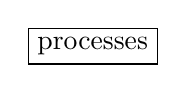
\begin{tikzpicture}
      \node [rectangle, text centered, draw=black]{processes};
    \end{tikzpicture},
    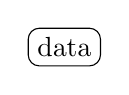
\begin{tikzpicture}
      \node [rectangle, rounded corners, text centered, draw=black]{data};
    \end{tikzpicture} and
    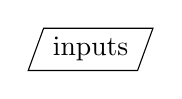
\begin{tikzpicture}
      \node [trapezium, trapezium left angle=70, trapezium right angle=110,
             text centered, draw=black]{inputs};
  \end{tikzpicture}}
  \label{figure:flow_chart}
\end{figure}

\section{Application}
\label{sec:application}

We have applied our benchmarking methodology to the QuickSpec and IsaCoSy MTE
tools, using version 0.2 of the TIP (Tons of Inductive Problems) theorem proving
benchmark as our ground truth corpus~\cite{claessen2015tip}.

To determine our benchmarking parameters we ran some initial tests on both tools
for a few samples sized between 1 and 100, for an hour each on our benchmarking
machine with a 3.2GHz dual-core Intel i5 processor with hyper-threading and 8GB
of RAM. Most QuickSpec runs either finished within 200 seconds or not at all,
and sizes above 20 mostly timed out. IsaCoSy mostly finished within 300 seconds
on sample sizes up to 4, but by size 8 was mostly timing out; its few successes
above this took thousands of seconds each, which we deemed infeasibly long.

Based on this we decided to benchmark sample sizes up to 20, since neither tool
seemed to perform well beyond that. The Speedup-Test protocol follows the
statistical ``rule of thumb'' of treating sample sizes $\leq$ 30 as ``small'',
so we pick 31 samples of each size in order to cross this threshold. This gave a
total of 1240 runs. To keep the benchmarking time down to a few days we chose a
timeout of 300 seconds, since that covered most of the successful QuickSpec and
IsaCoSy results we saw, and longer times gave rapidly diminishing
returns. During analysis, duplicate samples (caused by our requirement that
samples have a non-empty ground truth) were found and discarded, so only 14
samples of size 1 were used and 30 of size 2.

\subsection{Tons of Inductive Problems}
\label{sec:tip}

We chose the Tons of Inductive Problems (TIP) benchmark for our ground truth
since it satisfies the criteria specified in $\S$\ref{section:prep}: each
benchmark problem has standalone type and function definitions, making their
separation trivial; known examples from the software verification and inductive
theorem proving literature are included, ensuring relevance to those fields; the
format includes the higher-order functions and inductive datatypes we are
interested in; it is large enough to pose a challenge to current MTE tools; plus
it is accompanied by tooling to convert its custom format (an extension of
SMT-Lib~\cite{BarFT-SMTLIB}) into a variety of languages, including Haskell and
Isabelle.

We use TIP version 0.2 which contains 343 problems, each stating a single
property and together defining a total of 618 datatypes and 1498 functions. Most
of these are duplicates, since each problem (re\nobreakdash-)defines all of the
datatypes and functions it involves.

TIP datatypes can have several ``constructors'' (introduction forms) and
``destructors'' (elimination forms; field accessors). For example the type of
lists from Figure~\ref{figure:list_theory} can be defined in the TIP format as
follows:

\begin{samepage}
\begin{verbatim}
(declare-datatypes
  (a)                       ;; Type parameter (element type)
  ((List                    ;; Type name
     (Nil)                  ;; Constructor (nullary)
     (Cons                  ;; Constructor (binary)
       (head a)             ;; Field name and type
       (tail (List a))))))  ;; Field name and type
\end{verbatim}
\end{samepage}

Our target languages (Haskell and Isabelle) differ in the way they handle
constructors and destructors, which complicates comparisons. To avoid this, we
generate a new function for each constructor (via $\eta$-expansion) and
destructor (via pattern-matching) of the following form:

\begin{samepage}
\begin{verbatim}
(define-fun
  (par (a)                   ;; Type parameter
    (constructor-Cons        ;; Function name
      ((x a) (xs (List a)))  ;; Argument names and types
      (List a)               ;; Return type
      (as                    ;; Type annotation
        (Cons x xs)          ;; Return value
        (List a)))))         ;; Return type
\end{verbatim}
\end{samepage}

\begin{samepage}
\begin{verbatim}
(define-fun
  (par (a)                        ;; Type parameter
    (destructor-head              ;; Function name
      ((xs (List a)))             ;; Argument name and type
      a                           ;; Return type
      (match xs                   ;; Pattern-match
        (case (Cons h t) h)))))   ;; Return relevant field
\end{verbatim}
\end{samepage}

\begin{sloppypar}
  We rewrite the TIP properties (our ground truth) to reference these expanded
  forms instead of the raw constructors and destructors, and use these functions
  in our samples in lieu of the raw expressions. Note that these destructor
  wrappers are \emph{partial} functions (e.g. \texttt{destructor-head} and
  \texttt{destructor-tail} are undefined for the input \texttt{Nil}), which
  complicates their translation to proof assistants like Isabelle.
\end{sloppypar}

Another complication is TIP's ``native'' support for booleans and integers,
which allows numerals and symbols like \texttt{+} to appear without any
accompanying definition. To ensure consistency in the translations, we replace
all occurrences of such expressions with standard definitions written with the
``user-level'' \texttt{declare-datatypes} and \texttt{define-fun}
mechanisms.~\footnote{\texttt{Boolean} has \texttt{true} and \texttt{false}
  constructors; \texttt{Natural} has \texttt{zero} and \texttt{successor};
  \texttt{Integer} has unary \texttt{positive} and \texttt{negative}
  constructors taking \texttt{Natural}s, and a nullary \texttt{zero} for
  symmetry.}

When we add all of these generated types and functions to those in TIP, we get a
total of 3598 definitions. Removing $\alpha$-equivalent duplicates leaves 269,
and we choose to only sample from those 182 functions which are referenced by at
least one property (this removes ambiguity about which \emph{definitions} count
as interesting and which are just ``implementation details'' for other
definitions).

TIP comes with software to translate its definitions into Haskell and Isabelle
code, including comparison functions and random data generators suitable for
QuickCheck. We translate all 269 unique definitions into a single module/theory
which is imported on each run of the tools, although only those functions which
appear in the current sample are included in the signature and explored. We also
encode all names in hexadecimal to avoid problems with language-specific naming
rules, for example \texttt{add} becomes \texttt{global616464} (the prefix
distinguishes these from local variables and prevents names from beginning with
a digit). This ensures that the generated conjectures will be using the same
names as the ground truth, rather than some language-specific variant.

\subsection{QuickSpec}

We benchmarked QuickSpec version 0.9.6, a tool written in Haskell for
conjecturing equations involving Haskell functions, described in more detail in
$\S$\ref{sec:existing-tools}. In order to thoroughly benchmark QuickSpec, we
need to automate some of the decisions which are normally left up to the user:

\begin{sloppypar}
  \begin{itemize}
  \item We must decide what variables to include. We choose to add three
    variables for each type that appears as a function argument, except for
    types which have no QuickCheck data generators.
  \item We must \emph{monomorphise} all types. For example, functions like
    \texttt{constructor-Cons} are \emph{polymorphic}: they build lists of any
    element type, but we need to pick a specific type in order to know which
    random value generator to use. We resolve this (arbitrarily) by picking
    \texttt{Integer}.~\footnote{We pick \texttt{Integer} for variables of kind
      \texttt{*} (types); for kind \texttt{* -> *} (type constructors) we pick
      \texttt{[]} (Haskell's list type constructor). If these violate some
      type class constraint, we pick a suitable type non-deterministically from
      those in scope during compilation; if no suitable type is found, we give
      up and don't include that function.}
  \item Haskell functions are ``black boxes'', which QuickSpec can't compare
    during its exploration process. They are also curried, always taking one
    argument but potentially returning another function. QuickSpec lets us
    assign an arity to each function in the signature, from 0 to 5, so we pick
    the highest that is type-correct, since this avoids a proliferation of
    incomparable, partially-applied functions.
  \end{itemize}
\end{sloppypar}

\begin{figure}
  \centering
  %% Creator: Matplotlib, PGF backend
%%
%% To include the figure in your LaTeX document, write
%%   \input{<filename>.pgf}
%%
%% Make sure the required packages are loaded in your preamble
%%   \usepackage{pgf}
%%
%% Figures using additional raster images can only be included by \input if
%% they are in the same directory as the main LaTeX file. For loading figures
%% from other directories you can use the `import` package
%%   \usepackage{import}
%% and then include the figures with
%%   \import{<path to file>}{<filename>.pgf}
%%
%% Matplotlib used the following preamble
%%   \usepackage[utf8x]{inputenc}
%%   \usepackage[T1]{fontenc}
%%
\begingroup%
\makeatletter%
\begin{pgfpicture}%
\pgfpathrectangle{\pgfpointorigin}{\pgfqpoint{3.202355in}{1.216845in}}%
\pgfusepath{use as bounding box, clip}%
\begin{pgfscope}%
\pgfsetbuttcap%
\pgfsetmiterjoin%
\definecolor{currentfill}{rgb}{1.000000,1.000000,1.000000}%
\pgfsetfillcolor{currentfill}%
\pgfsetlinewidth{0.000000pt}%
\definecolor{currentstroke}{rgb}{1.000000,1.000000,1.000000}%
\pgfsetstrokecolor{currentstroke}%
\pgfsetdash{}{0pt}%
\pgfpathmoveto{\pgfqpoint{-0.000000in}{0.000000in}}%
\pgfpathlineto{\pgfqpoint{3.202355in}{0.000000in}}%
\pgfpathlineto{\pgfqpoint{3.202355in}{1.216845in}}%
\pgfpathlineto{\pgfqpoint{-0.000000in}{1.216845in}}%
\pgfpathclose%
\pgfusepath{fill}%
\end{pgfscope}%
\begin{pgfscope}%
\pgfsetbuttcap%
\pgfsetmiterjoin%
\definecolor{currentfill}{rgb}{1.000000,1.000000,1.000000}%
\pgfsetfillcolor{currentfill}%
\pgfsetlinewidth{0.000000pt}%
\definecolor{currentstroke}{rgb}{0.000000,0.000000,0.000000}%
\pgfsetstrokecolor{currentstroke}%
\pgfsetstrokeopacity{0.000000}%
\pgfsetdash{}{0pt}%
\pgfpathmoveto{\pgfqpoint{0.448843in}{0.362833in}}%
\pgfpathlineto{\pgfqpoint{3.202355in}{0.362833in}}%
\pgfpathlineto{\pgfqpoint{3.202355in}{1.066550in}}%
\pgfpathlineto{\pgfqpoint{0.448843in}{1.066550in}}%
\pgfpathclose%
\pgfusepath{fill}%
\end{pgfscope}%
\begin{pgfscope}%
\pgfsetbuttcap%
\pgfsetroundjoin%
\definecolor{currentfill}{rgb}{0.150000,0.150000,0.150000}%
\pgfsetfillcolor{currentfill}%
\pgfsetlinewidth{0.803000pt}%
\definecolor{currentstroke}{rgb}{0.150000,0.150000,0.150000}%
\pgfsetstrokecolor{currentstroke}%
\pgfsetdash{}{0pt}%
\pgfsys@defobject{currentmarker}{\pgfqpoint{0.000000in}{0.000000in}}{\pgfqpoint{0.000000in}{0.000000in}}{%
\pgfpathmoveto{\pgfqpoint{0.000000in}{0.000000in}}%
\pgfpathlineto{\pgfqpoint{0.000000in}{0.000000in}}%
\pgfusepath{stroke,fill}%
}%
\begin{pgfscope}%
\pgfsys@transformshift{0.517681in}{0.362833in}%
\pgfsys@useobject{currentmarker}{}%
\end{pgfscope}%
\end{pgfscope}%
\begin{pgfscope}%
\pgfsetbuttcap%
\pgfsetroundjoin%
\definecolor{currentfill}{rgb}{0.150000,0.150000,0.150000}%
\pgfsetfillcolor{currentfill}%
\pgfsetlinewidth{0.803000pt}%
\definecolor{currentstroke}{rgb}{0.150000,0.150000,0.150000}%
\pgfsetstrokecolor{currentstroke}%
\pgfsetdash{}{0pt}%
\pgfsys@defobject{currentmarker}{\pgfqpoint{0.000000in}{0.000000in}}{\pgfqpoint{0.000000in}{0.000000in}}{%
\pgfpathmoveto{\pgfqpoint{0.000000in}{0.000000in}}%
\pgfpathlineto{\pgfqpoint{0.000000in}{0.000000in}}%
\pgfusepath{stroke,fill}%
}%
\begin{pgfscope}%
\pgfsys@transformshift{0.517681in}{1.066550in}%
\pgfsys@useobject{currentmarker}{}%
\end{pgfscope}%
\end{pgfscope}%
\begin{pgfscope}%
\definecolor{textcolor}{rgb}{0.150000,0.150000,0.150000}%
\pgfsetstrokecolor{textcolor}%
\pgfsetfillcolor{textcolor}%
\pgftext[x=0.517681in,y=0.285055in,,top]{\color{textcolor}\sffamily\fontsize{8.000000}{9.600000}\selectfont 1}%
\end{pgfscope}%
\begin{pgfscope}%
\pgfsetbuttcap%
\pgfsetroundjoin%
\definecolor{currentfill}{rgb}{0.150000,0.150000,0.150000}%
\pgfsetfillcolor{currentfill}%
\pgfsetlinewidth{0.803000pt}%
\definecolor{currentstroke}{rgb}{0.150000,0.150000,0.150000}%
\pgfsetstrokecolor{currentstroke}%
\pgfsetdash{}{0pt}%
\pgfsys@defobject{currentmarker}{\pgfqpoint{0.000000in}{0.000000in}}{\pgfqpoint{0.000000in}{0.000000in}}{%
\pgfpathmoveto{\pgfqpoint{0.000000in}{0.000000in}}%
\pgfpathlineto{\pgfqpoint{0.000000in}{0.000000in}}%
\pgfusepath{stroke,fill}%
}%
\begin{pgfscope}%
\pgfsys@transformshift{0.655357in}{0.362833in}%
\pgfsys@useobject{currentmarker}{}%
\end{pgfscope}%
\end{pgfscope}%
\begin{pgfscope}%
\pgfsetbuttcap%
\pgfsetroundjoin%
\definecolor{currentfill}{rgb}{0.150000,0.150000,0.150000}%
\pgfsetfillcolor{currentfill}%
\pgfsetlinewidth{0.803000pt}%
\definecolor{currentstroke}{rgb}{0.150000,0.150000,0.150000}%
\pgfsetstrokecolor{currentstroke}%
\pgfsetdash{}{0pt}%
\pgfsys@defobject{currentmarker}{\pgfqpoint{0.000000in}{0.000000in}}{\pgfqpoint{0.000000in}{0.000000in}}{%
\pgfpathmoveto{\pgfqpoint{0.000000in}{0.000000in}}%
\pgfpathlineto{\pgfqpoint{0.000000in}{0.000000in}}%
\pgfusepath{stroke,fill}%
}%
\begin{pgfscope}%
\pgfsys@transformshift{0.655357in}{1.066550in}%
\pgfsys@useobject{currentmarker}{}%
\end{pgfscope}%
\end{pgfscope}%
\begin{pgfscope}%
\definecolor{textcolor}{rgb}{0.150000,0.150000,0.150000}%
\pgfsetstrokecolor{textcolor}%
\pgfsetfillcolor{textcolor}%
\pgftext[x=0.655357in,y=0.285055in,,top]{\color{textcolor}\sffamily\fontsize{8.000000}{9.600000}\selectfont 2}%
\end{pgfscope}%
\begin{pgfscope}%
\pgfsetbuttcap%
\pgfsetroundjoin%
\definecolor{currentfill}{rgb}{0.150000,0.150000,0.150000}%
\pgfsetfillcolor{currentfill}%
\pgfsetlinewidth{0.803000pt}%
\definecolor{currentstroke}{rgb}{0.150000,0.150000,0.150000}%
\pgfsetstrokecolor{currentstroke}%
\pgfsetdash{}{0pt}%
\pgfsys@defobject{currentmarker}{\pgfqpoint{0.000000in}{0.000000in}}{\pgfqpoint{0.000000in}{0.000000in}}{%
\pgfpathmoveto{\pgfqpoint{0.000000in}{0.000000in}}%
\pgfpathlineto{\pgfqpoint{0.000000in}{0.000000in}}%
\pgfusepath{stroke,fill}%
}%
\begin{pgfscope}%
\pgfsys@transformshift{0.793032in}{0.362833in}%
\pgfsys@useobject{currentmarker}{}%
\end{pgfscope}%
\end{pgfscope}%
\begin{pgfscope}%
\pgfsetbuttcap%
\pgfsetroundjoin%
\definecolor{currentfill}{rgb}{0.150000,0.150000,0.150000}%
\pgfsetfillcolor{currentfill}%
\pgfsetlinewidth{0.803000pt}%
\definecolor{currentstroke}{rgb}{0.150000,0.150000,0.150000}%
\pgfsetstrokecolor{currentstroke}%
\pgfsetdash{}{0pt}%
\pgfsys@defobject{currentmarker}{\pgfqpoint{0.000000in}{0.000000in}}{\pgfqpoint{0.000000in}{0.000000in}}{%
\pgfpathmoveto{\pgfqpoint{0.000000in}{0.000000in}}%
\pgfpathlineto{\pgfqpoint{0.000000in}{0.000000in}}%
\pgfusepath{stroke,fill}%
}%
\begin{pgfscope}%
\pgfsys@transformshift{0.793032in}{1.066550in}%
\pgfsys@useobject{currentmarker}{}%
\end{pgfscope}%
\end{pgfscope}%
\begin{pgfscope}%
\definecolor{textcolor}{rgb}{0.150000,0.150000,0.150000}%
\pgfsetstrokecolor{textcolor}%
\pgfsetfillcolor{textcolor}%
\pgftext[x=0.793032in,y=0.285055in,,top]{\color{textcolor}\sffamily\fontsize{8.000000}{9.600000}\selectfont 3}%
\end{pgfscope}%
\begin{pgfscope}%
\pgfsetbuttcap%
\pgfsetroundjoin%
\definecolor{currentfill}{rgb}{0.150000,0.150000,0.150000}%
\pgfsetfillcolor{currentfill}%
\pgfsetlinewidth{0.803000pt}%
\definecolor{currentstroke}{rgb}{0.150000,0.150000,0.150000}%
\pgfsetstrokecolor{currentstroke}%
\pgfsetdash{}{0pt}%
\pgfsys@defobject{currentmarker}{\pgfqpoint{0.000000in}{0.000000in}}{\pgfqpoint{0.000000in}{0.000000in}}{%
\pgfpathmoveto{\pgfqpoint{0.000000in}{0.000000in}}%
\pgfpathlineto{\pgfqpoint{0.000000in}{0.000000in}}%
\pgfusepath{stroke,fill}%
}%
\begin{pgfscope}%
\pgfsys@transformshift{0.930708in}{0.362833in}%
\pgfsys@useobject{currentmarker}{}%
\end{pgfscope}%
\end{pgfscope}%
\begin{pgfscope}%
\pgfsetbuttcap%
\pgfsetroundjoin%
\definecolor{currentfill}{rgb}{0.150000,0.150000,0.150000}%
\pgfsetfillcolor{currentfill}%
\pgfsetlinewidth{0.803000pt}%
\definecolor{currentstroke}{rgb}{0.150000,0.150000,0.150000}%
\pgfsetstrokecolor{currentstroke}%
\pgfsetdash{}{0pt}%
\pgfsys@defobject{currentmarker}{\pgfqpoint{0.000000in}{0.000000in}}{\pgfqpoint{0.000000in}{0.000000in}}{%
\pgfpathmoveto{\pgfqpoint{0.000000in}{0.000000in}}%
\pgfpathlineto{\pgfqpoint{0.000000in}{0.000000in}}%
\pgfusepath{stroke,fill}%
}%
\begin{pgfscope}%
\pgfsys@transformshift{0.930708in}{1.066550in}%
\pgfsys@useobject{currentmarker}{}%
\end{pgfscope}%
\end{pgfscope}%
\begin{pgfscope}%
\definecolor{textcolor}{rgb}{0.150000,0.150000,0.150000}%
\pgfsetstrokecolor{textcolor}%
\pgfsetfillcolor{textcolor}%
\pgftext[x=0.930708in,y=0.285055in,,top]{\color{textcolor}\sffamily\fontsize{8.000000}{9.600000}\selectfont 4}%
\end{pgfscope}%
\begin{pgfscope}%
\pgfsetbuttcap%
\pgfsetroundjoin%
\definecolor{currentfill}{rgb}{0.150000,0.150000,0.150000}%
\pgfsetfillcolor{currentfill}%
\pgfsetlinewidth{0.803000pt}%
\definecolor{currentstroke}{rgb}{0.150000,0.150000,0.150000}%
\pgfsetstrokecolor{currentstroke}%
\pgfsetdash{}{0pt}%
\pgfsys@defobject{currentmarker}{\pgfqpoint{0.000000in}{0.000000in}}{\pgfqpoint{0.000000in}{0.000000in}}{%
\pgfpathmoveto{\pgfqpoint{0.000000in}{0.000000in}}%
\pgfpathlineto{\pgfqpoint{0.000000in}{0.000000in}}%
\pgfusepath{stroke,fill}%
}%
\begin{pgfscope}%
\pgfsys@transformshift{1.068384in}{0.362833in}%
\pgfsys@useobject{currentmarker}{}%
\end{pgfscope}%
\end{pgfscope}%
\begin{pgfscope}%
\pgfsetbuttcap%
\pgfsetroundjoin%
\definecolor{currentfill}{rgb}{0.150000,0.150000,0.150000}%
\pgfsetfillcolor{currentfill}%
\pgfsetlinewidth{0.803000pt}%
\definecolor{currentstroke}{rgb}{0.150000,0.150000,0.150000}%
\pgfsetstrokecolor{currentstroke}%
\pgfsetdash{}{0pt}%
\pgfsys@defobject{currentmarker}{\pgfqpoint{0.000000in}{0.000000in}}{\pgfqpoint{0.000000in}{0.000000in}}{%
\pgfpathmoveto{\pgfqpoint{0.000000in}{0.000000in}}%
\pgfpathlineto{\pgfqpoint{0.000000in}{0.000000in}}%
\pgfusepath{stroke,fill}%
}%
\begin{pgfscope}%
\pgfsys@transformshift{1.068384in}{1.066550in}%
\pgfsys@useobject{currentmarker}{}%
\end{pgfscope}%
\end{pgfscope}%
\begin{pgfscope}%
\definecolor{textcolor}{rgb}{0.150000,0.150000,0.150000}%
\pgfsetstrokecolor{textcolor}%
\pgfsetfillcolor{textcolor}%
\pgftext[x=1.068384in,y=0.285055in,,top]{\color{textcolor}\sffamily\fontsize{8.000000}{9.600000}\selectfont 5}%
\end{pgfscope}%
\begin{pgfscope}%
\pgfsetbuttcap%
\pgfsetroundjoin%
\definecolor{currentfill}{rgb}{0.150000,0.150000,0.150000}%
\pgfsetfillcolor{currentfill}%
\pgfsetlinewidth{0.803000pt}%
\definecolor{currentstroke}{rgb}{0.150000,0.150000,0.150000}%
\pgfsetstrokecolor{currentstroke}%
\pgfsetdash{}{0pt}%
\pgfsys@defobject{currentmarker}{\pgfqpoint{0.000000in}{0.000000in}}{\pgfqpoint{0.000000in}{0.000000in}}{%
\pgfpathmoveto{\pgfqpoint{0.000000in}{0.000000in}}%
\pgfpathlineto{\pgfqpoint{0.000000in}{0.000000in}}%
\pgfusepath{stroke,fill}%
}%
\begin{pgfscope}%
\pgfsys@transformshift{1.206059in}{0.362833in}%
\pgfsys@useobject{currentmarker}{}%
\end{pgfscope}%
\end{pgfscope}%
\begin{pgfscope}%
\pgfsetbuttcap%
\pgfsetroundjoin%
\definecolor{currentfill}{rgb}{0.150000,0.150000,0.150000}%
\pgfsetfillcolor{currentfill}%
\pgfsetlinewidth{0.803000pt}%
\definecolor{currentstroke}{rgb}{0.150000,0.150000,0.150000}%
\pgfsetstrokecolor{currentstroke}%
\pgfsetdash{}{0pt}%
\pgfsys@defobject{currentmarker}{\pgfqpoint{0.000000in}{0.000000in}}{\pgfqpoint{0.000000in}{0.000000in}}{%
\pgfpathmoveto{\pgfqpoint{0.000000in}{0.000000in}}%
\pgfpathlineto{\pgfqpoint{0.000000in}{0.000000in}}%
\pgfusepath{stroke,fill}%
}%
\begin{pgfscope}%
\pgfsys@transformshift{1.206059in}{1.066550in}%
\pgfsys@useobject{currentmarker}{}%
\end{pgfscope}%
\end{pgfscope}%
\begin{pgfscope}%
\definecolor{textcolor}{rgb}{0.150000,0.150000,0.150000}%
\pgfsetstrokecolor{textcolor}%
\pgfsetfillcolor{textcolor}%
\pgftext[x=1.206059in,y=0.285055in,,top]{\color{textcolor}\sffamily\fontsize{8.000000}{9.600000}\selectfont 6}%
\end{pgfscope}%
\begin{pgfscope}%
\pgfsetbuttcap%
\pgfsetroundjoin%
\definecolor{currentfill}{rgb}{0.150000,0.150000,0.150000}%
\pgfsetfillcolor{currentfill}%
\pgfsetlinewidth{0.803000pt}%
\definecolor{currentstroke}{rgb}{0.150000,0.150000,0.150000}%
\pgfsetstrokecolor{currentstroke}%
\pgfsetdash{}{0pt}%
\pgfsys@defobject{currentmarker}{\pgfqpoint{0.000000in}{0.000000in}}{\pgfqpoint{0.000000in}{0.000000in}}{%
\pgfpathmoveto{\pgfqpoint{0.000000in}{0.000000in}}%
\pgfpathlineto{\pgfqpoint{0.000000in}{0.000000in}}%
\pgfusepath{stroke,fill}%
}%
\begin{pgfscope}%
\pgfsys@transformshift{1.343735in}{0.362833in}%
\pgfsys@useobject{currentmarker}{}%
\end{pgfscope}%
\end{pgfscope}%
\begin{pgfscope}%
\pgfsetbuttcap%
\pgfsetroundjoin%
\definecolor{currentfill}{rgb}{0.150000,0.150000,0.150000}%
\pgfsetfillcolor{currentfill}%
\pgfsetlinewidth{0.803000pt}%
\definecolor{currentstroke}{rgb}{0.150000,0.150000,0.150000}%
\pgfsetstrokecolor{currentstroke}%
\pgfsetdash{}{0pt}%
\pgfsys@defobject{currentmarker}{\pgfqpoint{0.000000in}{0.000000in}}{\pgfqpoint{0.000000in}{0.000000in}}{%
\pgfpathmoveto{\pgfqpoint{0.000000in}{0.000000in}}%
\pgfpathlineto{\pgfqpoint{0.000000in}{0.000000in}}%
\pgfusepath{stroke,fill}%
}%
\begin{pgfscope}%
\pgfsys@transformshift{1.343735in}{1.066550in}%
\pgfsys@useobject{currentmarker}{}%
\end{pgfscope}%
\end{pgfscope}%
\begin{pgfscope}%
\definecolor{textcolor}{rgb}{0.150000,0.150000,0.150000}%
\pgfsetstrokecolor{textcolor}%
\pgfsetfillcolor{textcolor}%
\pgftext[x=1.343735in,y=0.285055in,,top]{\color{textcolor}\sffamily\fontsize{8.000000}{9.600000}\selectfont 7}%
\end{pgfscope}%
\begin{pgfscope}%
\pgfsetbuttcap%
\pgfsetroundjoin%
\definecolor{currentfill}{rgb}{0.150000,0.150000,0.150000}%
\pgfsetfillcolor{currentfill}%
\pgfsetlinewidth{0.803000pt}%
\definecolor{currentstroke}{rgb}{0.150000,0.150000,0.150000}%
\pgfsetstrokecolor{currentstroke}%
\pgfsetdash{}{0pt}%
\pgfsys@defobject{currentmarker}{\pgfqpoint{0.000000in}{0.000000in}}{\pgfqpoint{0.000000in}{0.000000in}}{%
\pgfpathmoveto{\pgfqpoint{0.000000in}{0.000000in}}%
\pgfpathlineto{\pgfqpoint{0.000000in}{0.000000in}}%
\pgfusepath{stroke,fill}%
}%
\begin{pgfscope}%
\pgfsys@transformshift{1.481410in}{0.362833in}%
\pgfsys@useobject{currentmarker}{}%
\end{pgfscope}%
\end{pgfscope}%
\begin{pgfscope}%
\pgfsetbuttcap%
\pgfsetroundjoin%
\definecolor{currentfill}{rgb}{0.150000,0.150000,0.150000}%
\pgfsetfillcolor{currentfill}%
\pgfsetlinewidth{0.803000pt}%
\definecolor{currentstroke}{rgb}{0.150000,0.150000,0.150000}%
\pgfsetstrokecolor{currentstroke}%
\pgfsetdash{}{0pt}%
\pgfsys@defobject{currentmarker}{\pgfqpoint{0.000000in}{0.000000in}}{\pgfqpoint{0.000000in}{0.000000in}}{%
\pgfpathmoveto{\pgfqpoint{0.000000in}{0.000000in}}%
\pgfpathlineto{\pgfqpoint{0.000000in}{0.000000in}}%
\pgfusepath{stroke,fill}%
}%
\begin{pgfscope}%
\pgfsys@transformshift{1.481410in}{1.066550in}%
\pgfsys@useobject{currentmarker}{}%
\end{pgfscope}%
\end{pgfscope}%
\begin{pgfscope}%
\definecolor{textcolor}{rgb}{0.150000,0.150000,0.150000}%
\pgfsetstrokecolor{textcolor}%
\pgfsetfillcolor{textcolor}%
\pgftext[x=1.481410in,y=0.285055in,,top]{\color{textcolor}\sffamily\fontsize{8.000000}{9.600000}\selectfont 8}%
\end{pgfscope}%
\begin{pgfscope}%
\pgfsetbuttcap%
\pgfsetroundjoin%
\definecolor{currentfill}{rgb}{0.150000,0.150000,0.150000}%
\pgfsetfillcolor{currentfill}%
\pgfsetlinewidth{0.803000pt}%
\definecolor{currentstroke}{rgb}{0.150000,0.150000,0.150000}%
\pgfsetstrokecolor{currentstroke}%
\pgfsetdash{}{0pt}%
\pgfsys@defobject{currentmarker}{\pgfqpoint{0.000000in}{0.000000in}}{\pgfqpoint{0.000000in}{0.000000in}}{%
\pgfpathmoveto{\pgfqpoint{0.000000in}{0.000000in}}%
\pgfpathlineto{\pgfqpoint{0.000000in}{0.000000in}}%
\pgfusepath{stroke,fill}%
}%
\begin{pgfscope}%
\pgfsys@transformshift{1.619086in}{0.362833in}%
\pgfsys@useobject{currentmarker}{}%
\end{pgfscope}%
\end{pgfscope}%
\begin{pgfscope}%
\pgfsetbuttcap%
\pgfsetroundjoin%
\definecolor{currentfill}{rgb}{0.150000,0.150000,0.150000}%
\pgfsetfillcolor{currentfill}%
\pgfsetlinewidth{0.803000pt}%
\definecolor{currentstroke}{rgb}{0.150000,0.150000,0.150000}%
\pgfsetstrokecolor{currentstroke}%
\pgfsetdash{}{0pt}%
\pgfsys@defobject{currentmarker}{\pgfqpoint{0.000000in}{0.000000in}}{\pgfqpoint{0.000000in}{0.000000in}}{%
\pgfpathmoveto{\pgfqpoint{0.000000in}{0.000000in}}%
\pgfpathlineto{\pgfqpoint{0.000000in}{0.000000in}}%
\pgfusepath{stroke,fill}%
}%
\begin{pgfscope}%
\pgfsys@transformshift{1.619086in}{1.066550in}%
\pgfsys@useobject{currentmarker}{}%
\end{pgfscope}%
\end{pgfscope}%
\begin{pgfscope}%
\definecolor{textcolor}{rgb}{0.150000,0.150000,0.150000}%
\pgfsetstrokecolor{textcolor}%
\pgfsetfillcolor{textcolor}%
\pgftext[x=1.619086in,y=0.285055in,,top]{\color{textcolor}\sffamily\fontsize{8.000000}{9.600000}\selectfont 9}%
\end{pgfscope}%
\begin{pgfscope}%
\pgfsetbuttcap%
\pgfsetroundjoin%
\definecolor{currentfill}{rgb}{0.150000,0.150000,0.150000}%
\pgfsetfillcolor{currentfill}%
\pgfsetlinewidth{0.803000pt}%
\definecolor{currentstroke}{rgb}{0.150000,0.150000,0.150000}%
\pgfsetstrokecolor{currentstroke}%
\pgfsetdash{}{0pt}%
\pgfsys@defobject{currentmarker}{\pgfqpoint{0.000000in}{0.000000in}}{\pgfqpoint{0.000000in}{0.000000in}}{%
\pgfpathmoveto{\pgfqpoint{0.000000in}{0.000000in}}%
\pgfpathlineto{\pgfqpoint{0.000000in}{0.000000in}}%
\pgfusepath{stroke,fill}%
}%
\begin{pgfscope}%
\pgfsys@transformshift{1.756762in}{0.362833in}%
\pgfsys@useobject{currentmarker}{}%
\end{pgfscope}%
\end{pgfscope}%
\begin{pgfscope}%
\pgfsetbuttcap%
\pgfsetroundjoin%
\definecolor{currentfill}{rgb}{0.150000,0.150000,0.150000}%
\pgfsetfillcolor{currentfill}%
\pgfsetlinewidth{0.803000pt}%
\definecolor{currentstroke}{rgb}{0.150000,0.150000,0.150000}%
\pgfsetstrokecolor{currentstroke}%
\pgfsetdash{}{0pt}%
\pgfsys@defobject{currentmarker}{\pgfqpoint{0.000000in}{0.000000in}}{\pgfqpoint{0.000000in}{0.000000in}}{%
\pgfpathmoveto{\pgfqpoint{0.000000in}{0.000000in}}%
\pgfpathlineto{\pgfqpoint{0.000000in}{0.000000in}}%
\pgfusepath{stroke,fill}%
}%
\begin{pgfscope}%
\pgfsys@transformshift{1.756762in}{1.066550in}%
\pgfsys@useobject{currentmarker}{}%
\end{pgfscope}%
\end{pgfscope}%
\begin{pgfscope}%
\definecolor{textcolor}{rgb}{0.150000,0.150000,0.150000}%
\pgfsetstrokecolor{textcolor}%
\pgfsetfillcolor{textcolor}%
\pgftext[x=1.756762in,y=0.285055in,,top]{\color{textcolor}\sffamily\fontsize{8.000000}{9.600000}\selectfont 10}%
\end{pgfscope}%
\begin{pgfscope}%
\pgfsetbuttcap%
\pgfsetroundjoin%
\definecolor{currentfill}{rgb}{0.150000,0.150000,0.150000}%
\pgfsetfillcolor{currentfill}%
\pgfsetlinewidth{0.803000pt}%
\definecolor{currentstroke}{rgb}{0.150000,0.150000,0.150000}%
\pgfsetstrokecolor{currentstroke}%
\pgfsetdash{}{0pt}%
\pgfsys@defobject{currentmarker}{\pgfqpoint{0.000000in}{0.000000in}}{\pgfqpoint{0.000000in}{0.000000in}}{%
\pgfpathmoveto{\pgfqpoint{0.000000in}{0.000000in}}%
\pgfpathlineto{\pgfqpoint{0.000000in}{0.000000in}}%
\pgfusepath{stroke,fill}%
}%
\begin{pgfscope}%
\pgfsys@transformshift{1.894437in}{0.362833in}%
\pgfsys@useobject{currentmarker}{}%
\end{pgfscope}%
\end{pgfscope}%
\begin{pgfscope}%
\pgfsetbuttcap%
\pgfsetroundjoin%
\definecolor{currentfill}{rgb}{0.150000,0.150000,0.150000}%
\pgfsetfillcolor{currentfill}%
\pgfsetlinewidth{0.803000pt}%
\definecolor{currentstroke}{rgb}{0.150000,0.150000,0.150000}%
\pgfsetstrokecolor{currentstroke}%
\pgfsetdash{}{0pt}%
\pgfsys@defobject{currentmarker}{\pgfqpoint{0.000000in}{0.000000in}}{\pgfqpoint{0.000000in}{0.000000in}}{%
\pgfpathmoveto{\pgfqpoint{0.000000in}{0.000000in}}%
\pgfpathlineto{\pgfqpoint{0.000000in}{0.000000in}}%
\pgfusepath{stroke,fill}%
}%
\begin{pgfscope}%
\pgfsys@transformshift{1.894437in}{1.066550in}%
\pgfsys@useobject{currentmarker}{}%
\end{pgfscope}%
\end{pgfscope}%
\begin{pgfscope}%
\definecolor{textcolor}{rgb}{0.150000,0.150000,0.150000}%
\pgfsetstrokecolor{textcolor}%
\pgfsetfillcolor{textcolor}%
\pgftext[x=1.894437in,y=0.285055in,,top]{\color{textcolor}\sffamily\fontsize{8.000000}{9.600000}\selectfont 11}%
\end{pgfscope}%
\begin{pgfscope}%
\pgfsetbuttcap%
\pgfsetroundjoin%
\definecolor{currentfill}{rgb}{0.150000,0.150000,0.150000}%
\pgfsetfillcolor{currentfill}%
\pgfsetlinewidth{0.803000pt}%
\definecolor{currentstroke}{rgb}{0.150000,0.150000,0.150000}%
\pgfsetstrokecolor{currentstroke}%
\pgfsetdash{}{0pt}%
\pgfsys@defobject{currentmarker}{\pgfqpoint{0.000000in}{0.000000in}}{\pgfqpoint{0.000000in}{0.000000in}}{%
\pgfpathmoveto{\pgfqpoint{0.000000in}{0.000000in}}%
\pgfpathlineto{\pgfqpoint{0.000000in}{0.000000in}}%
\pgfusepath{stroke,fill}%
}%
\begin{pgfscope}%
\pgfsys@transformshift{2.032113in}{0.362833in}%
\pgfsys@useobject{currentmarker}{}%
\end{pgfscope}%
\end{pgfscope}%
\begin{pgfscope}%
\pgfsetbuttcap%
\pgfsetroundjoin%
\definecolor{currentfill}{rgb}{0.150000,0.150000,0.150000}%
\pgfsetfillcolor{currentfill}%
\pgfsetlinewidth{0.803000pt}%
\definecolor{currentstroke}{rgb}{0.150000,0.150000,0.150000}%
\pgfsetstrokecolor{currentstroke}%
\pgfsetdash{}{0pt}%
\pgfsys@defobject{currentmarker}{\pgfqpoint{0.000000in}{0.000000in}}{\pgfqpoint{0.000000in}{0.000000in}}{%
\pgfpathmoveto{\pgfqpoint{0.000000in}{0.000000in}}%
\pgfpathlineto{\pgfqpoint{0.000000in}{0.000000in}}%
\pgfusepath{stroke,fill}%
}%
\begin{pgfscope}%
\pgfsys@transformshift{2.032113in}{1.066550in}%
\pgfsys@useobject{currentmarker}{}%
\end{pgfscope}%
\end{pgfscope}%
\begin{pgfscope}%
\definecolor{textcolor}{rgb}{0.150000,0.150000,0.150000}%
\pgfsetstrokecolor{textcolor}%
\pgfsetfillcolor{textcolor}%
\pgftext[x=2.032113in,y=0.285055in,,top]{\color{textcolor}\sffamily\fontsize{8.000000}{9.600000}\selectfont 12}%
\end{pgfscope}%
\begin{pgfscope}%
\pgfsetbuttcap%
\pgfsetroundjoin%
\definecolor{currentfill}{rgb}{0.150000,0.150000,0.150000}%
\pgfsetfillcolor{currentfill}%
\pgfsetlinewidth{0.803000pt}%
\definecolor{currentstroke}{rgb}{0.150000,0.150000,0.150000}%
\pgfsetstrokecolor{currentstroke}%
\pgfsetdash{}{0pt}%
\pgfsys@defobject{currentmarker}{\pgfqpoint{0.000000in}{0.000000in}}{\pgfqpoint{0.000000in}{0.000000in}}{%
\pgfpathmoveto{\pgfqpoint{0.000000in}{0.000000in}}%
\pgfpathlineto{\pgfqpoint{0.000000in}{0.000000in}}%
\pgfusepath{stroke,fill}%
}%
\begin{pgfscope}%
\pgfsys@transformshift{2.169788in}{0.362833in}%
\pgfsys@useobject{currentmarker}{}%
\end{pgfscope}%
\end{pgfscope}%
\begin{pgfscope}%
\pgfsetbuttcap%
\pgfsetroundjoin%
\definecolor{currentfill}{rgb}{0.150000,0.150000,0.150000}%
\pgfsetfillcolor{currentfill}%
\pgfsetlinewidth{0.803000pt}%
\definecolor{currentstroke}{rgb}{0.150000,0.150000,0.150000}%
\pgfsetstrokecolor{currentstroke}%
\pgfsetdash{}{0pt}%
\pgfsys@defobject{currentmarker}{\pgfqpoint{0.000000in}{0.000000in}}{\pgfqpoint{0.000000in}{0.000000in}}{%
\pgfpathmoveto{\pgfqpoint{0.000000in}{0.000000in}}%
\pgfpathlineto{\pgfqpoint{0.000000in}{0.000000in}}%
\pgfusepath{stroke,fill}%
}%
\begin{pgfscope}%
\pgfsys@transformshift{2.169788in}{1.066550in}%
\pgfsys@useobject{currentmarker}{}%
\end{pgfscope}%
\end{pgfscope}%
\begin{pgfscope}%
\definecolor{textcolor}{rgb}{0.150000,0.150000,0.150000}%
\pgfsetstrokecolor{textcolor}%
\pgfsetfillcolor{textcolor}%
\pgftext[x=2.169788in,y=0.285055in,,top]{\color{textcolor}\sffamily\fontsize{8.000000}{9.600000}\selectfont 13}%
\end{pgfscope}%
\begin{pgfscope}%
\pgfsetbuttcap%
\pgfsetroundjoin%
\definecolor{currentfill}{rgb}{0.150000,0.150000,0.150000}%
\pgfsetfillcolor{currentfill}%
\pgfsetlinewidth{0.803000pt}%
\definecolor{currentstroke}{rgb}{0.150000,0.150000,0.150000}%
\pgfsetstrokecolor{currentstroke}%
\pgfsetdash{}{0pt}%
\pgfsys@defobject{currentmarker}{\pgfqpoint{0.000000in}{0.000000in}}{\pgfqpoint{0.000000in}{0.000000in}}{%
\pgfpathmoveto{\pgfqpoint{0.000000in}{0.000000in}}%
\pgfpathlineto{\pgfqpoint{0.000000in}{0.000000in}}%
\pgfusepath{stroke,fill}%
}%
\begin{pgfscope}%
\pgfsys@transformshift{2.307464in}{0.362833in}%
\pgfsys@useobject{currentmarker}{}%
\end{pgfscope}%
\end{pgfscope}%
\begin{pgfscope}%
\pgfsetbuttcap%
\pgfsetroundjoin%
\definecolor{currentfill}{rgb}{0.150000,0.150000,0.150000}%
\pgfsetfillcolor{currentfill}%
\pgfsetlinewidth{0.803000pt}%
\definecolor{currentstroke}{rgb}{0.150000,0.150000,0.150000}%
\pgfsetstrokecolor{currentstroke}%
\pgfsetdash{}{0pt}%
\pgfsys@defobject{currentmarker}{\pgfqpoint{0.000000in}{0.000000in}}{\pgfqpoint{0.000000in}{0.000000in}}{%
\pgfpathmoveto{\pgfqpoint{0.000000in}{0.000000in}}%
\pgfpathlineto{\pgfqpoint{0.000000in}{0.000000in}}%
\pgfusepath{stroke,fill}%
}%
\begin{pgfscope}%
\pgfsys@transformshift{2.307464in}{1.066550in}%
\pgfsys@useobject{currentmarker}{}%
\end{pgfscope}%
\end{pgfscope}%
\begin{pgfscope}%
\definecolor{textcolor}{rgb}{0.150000,0.150000,0.150000}%
\pgfsetstrokecolor{textcolor}%
\pgfsetfillcolor{textcolor}%
\pgftext[x=2.307464in,y=0.285055in,,top]{\color{textcolor}\sffamily\fontsize{8.000000}{9.600000}\selectfont 14}%
\end{pgfscope}%
\begin{pgfscope}%
\pgfsetbuttcap%
\pgfsetroundjoin%
\definecolor{currentfill}{rgb}{0.150000,0.150000,0.150000}%
\pgfsetfillcolor{currentfill}%
\pgfsetlinewidth{0.803000pt}%
\definecolor{currentstroke}{rgb}{0.150000,0.150000,0.150000}%
\pgfsetstrokecolor{currentstroke}%
\pgfsetdash{}{0pt}%
\pgfsys@defobject{currentmarker}{\pgfqpoint{0.000000in}{0.000000in}}{\pgfqpoint{0.000000in}{0.000000in}}{%
\pgfpathmoveto{\pgfqpoint{0.000000in}{0.000000in}}%
\pgfpathlineto{\pgfqpoint{0.000000in}{0.000000in}}%
\pgfusepath{stroke,fill}%
}%
\begin{pgfscope}%
\pgfsys@transformshift{2.445140in}{0.362833in}%
\pgfsys@useobject{currentmarker}{}%
\end{pgfscope}%
\end{pgfscope}%
\begin{pgfscope}%
\pgfsetbuttcap%
\pgfsetroundjoin%
\definecolor{currentfill}{rgb}{0.150000,0.150000,0.150000}%
\pgfsetfillcolor{currentfill}%
\pgfsetlinewidth{0.803000pt}%
\definecolor{currentstroke}{rgb}{0.150000,0.150000,0.150000}%
\pgfsetstrokecolor{currentstroke}%
\pgfsetdash{}{0pt}%
\pgfsys@defobject{currentmarker}{\pgfqpoint{0.000000in}{0.000000in}}{\pgfqpoint{0.000000in}{0.000000in}}{%
\pgfpathmoveto{\pgfqpoint{0.000000in}{0.000000in}}%
\pgfpathlineto{\pgfqpoint{0.000000in}{0.000000in}}%
\pgfusepath{stroke,fill}%
}%
\begin{pgfscope}%
\pgfsys@transformshift{2.445140in}{1.066550in}%
\pgfsys@useobject{currentmarker}{}%
\end{pgfscope}%
\end{pgfscope}%
\begin{pgfscope}%
\definecolor{textcolor}{rgb}{0.150000,0.150000,0.150000}%
\pgfsetstrokecolor{textcolor}%
\pgfsetfillcolor{textcolor}%
\pgftext[x=2.445140in,y=0.285055in,,top]{\color{textcolor}\sffamily\fontsize{8.000000}{9.600000}\selectfont 15}%
\end{pgfscope}%
\begin{pgfscope}%
\pgfsetbuttcap%
\pgfsetroundjoin%
\definecolor{currentfill}{rgb}{0.150000,0.150000,0.150000}%
\pgfsetfillcolor{currentfill}%
\pgfsetlinewidth{0.803000pt}%
\definecolor{currentstroke}{rgb}{0.150000,0.150000,0.150000}%
\pgfsetstrokecolor{currentstroke}%
\pgfsetdash{}{0pt}%
\pgfsys@defobject{currentmarker}{\pgfqpoint{0.000000in}{0.000000in}}{\pgfqpoint{0.000000in}{0.000000in}}{%
\pgfpathmoveto{\pgfqpoint{0.000000in}{0.000000in}}%
\pgfpathlineto{\pgfqpoint{0.000000in}{0.000000in}}%
\pgfusepath{stroke,fill}%
}%
\begin{pgfscope}%
\pgfsys@transformshift{2.582815in}{0.362833in}%
\pgfsys@useobject{currentmarker}{}%
\end{pgfscope}%
\end{pgfscope}%
\begin{pgfscope}%
\pgfsetbuttcap%
\pgfsetroundjoin%
\definecolor{currentfill}{rgb}{0.150000,0.150000,0.150000}%
\pgfsetfillcolor{currentfill}%
\pgfsetlinewidth{0.803000pt}%
\definecolor{currentstroke}{rgb}{0.150000,0.150000,0.150000}%
\pgfsetstrokecolor{currentstroke}%
\pgfsetdash{}{0pt}%
\pgfsys@defobject{currentmarker}{\pgfqpoint{0.000000in}{0.000000in}}{\pgfqpoint{0.000000in}{0.000000in}}{%
\pgfpathmoveto{\pgfqpoint{0.000000in}{0.000000in}}%
\pgfpathlineto{\pgfqpoint{0.000000in}{0.000000in}}%
\pgfusepath{stroke,fill}%
}%
\begin{pgfscope}%
\pgfsys@transformshift{2.582815in}{1.066550in}%
\pgfsys@useobject{currentmarker}{}%
\end{pgfscope}%
\end{pgfscope}%
\begin{pgfscope}%
\definecolor{textcolor}{rgb}{0.150000,0.150000,0.150000}%
\pgfsetstrokecolor{textcolor}%
\pgfsetfillcolor{textcolor}%
\pgftext[x=2.582815in,y=0.285055in,,top]{\color{textcolor}\sffamily\fontsize{8.000000}{9.600000}\selectfont 16}%
\end{pgfscope}%
\begin{pgfscope}%
\pgfsetbuttcap%
\pgfsetroundjoin%
\definecolor{currentfill}{rgb}{0.150000,0.150000,0.150000}%
\pgfsetfillcolor{currentfill}%
\pgfsetlinewidth{0.803000pt}%
\definecolor{currentstroke}{rgb}{0.150000,0.150000,0.150000}%
\pgfsetstrokecolor{currentstroke}%
\pgfsetdash{}{0pt}%
\pgfsys@defobject{currentmarker}{\pgfqpoint{0.000000in}{0.000000in}}{\pgfqpoint{0.000000in}{0.000000in}}{%
\pgfpathmoveto{\pgfqpoint{0.000000in}{0.000000in}}%
\pgfpathlineto{\pgfqpoint{0.000000in}{0.000000in}}%
\pgfusepath{stroke,fill}%
}%
\begin{pgfscope}%
\pgfsys@transformshift{2.720491in}{0.362833in}%
\pgfsys@useobject{currentmarker}{}%
\end{pgfscope}%
\end{pgfscope}%
\begin{pgfscope}%
\pgfsetbuttcap%
\pgfsetroundjoin%
\definecolor{currentfill}{rgb}{0.150000,0.150000,0.150000}%
\pgfsetfillcolor{currentfill}%
\pgfsetlinewidth{0.803000pt}%
\definecolor{currentstroke}{rgb}{0.150000,0.150000,0.150000}%
\pgfsetstrokecolor{currentstroke}%
\pgfsetdash{}{0pt}%
\pgfsys@defobject{currentmarker}{\pgfqpoint{0.000000in}{0.000000in}}{\pgfqpoint{0.000000in}{0.000000in}}{%
\pgfpathmoveto{\pgfqpoint{0.000000in}{0.000000in}}%
\pgfpathlineto{\pgfqpoint{0.000000in}{0.000000in}}%
\pgfusepath{stroke,fill}%
}%
\begin{pgfscope}%
\pgfsys@transformshift{2.720491in}{1.066550in}%
\pgfsys@useobject{currentmarker}{}%
\end{pgfscope}%
\end{pgfscope}%
\begin{pgfscope}%
\definecolor{textcolor}{rgb}{0.150000,0.150000,0.150000}%
\pgfsetstrokecolor{textcolor}%
\pgfsetfillcolor{textcolor}%
\pgftext[x=2.720491in,y=0.285055in,,top]{\color{textcolor}\sffamily\fontsize{8.000000}{9.600000}\selectfont 17}%
\end{pgfscope}%
\begin{pgfscope}%
\pgfsetbuttcap%
\pgfsetroundjoin%
\definecolor{currentfill}{rgb}{0.150000,0.150000,0.150000}%
\pgfsetfillcolor{currentfill}%
\pgfsetlinewidth{0.803000pt}%
\definecolor{currentstroke}{rgb}{0.150000,0.150000,0.150000}%
\pgfsetstrokecolor{currentstroke}%
\pgfsetdash{}{0pt}%
\pgfsys@defobject{currentmarker}{\pgfqpoint{0.000000in}{0.000000in}}{\pgfqpoint{0.000000in}{0.000000in}}{%
\pgfpathmoveto{\pgfqpoint{0.000000in}{0.000000in}}%
\pgfpathlineto{\pgfqpoint{0.000000in}{0.000000in}}%
\pgfusepath{stroke,fill}%
}%
\begin{pgfscope}%
\pgfsys@transformshift{2.858166in}{0.362833in}%
\pgfsys@useobject{currentmarker}{}%
\end{pgfscope}%
\end{pgfscope}%
\begin{pgfscope}%
\pgfsetbuttcap%
\pgfsetroundjoin%
\definecolor{currentfill}{rgb}{0.150000,0.150000,0.150000}%
\pgfsetfillcolor{currentfill}%
\pgfsetlinewidth{0.803000pt}%
\definecolor{currentstroke}{rgb}{0.150000,0.150000,0.150000}%
\pgfsetstrokecolor{currentstroke}%
\pgfsetdash{}{0pt}%
\pgfsys@defobject{currentmarker}{\pgfqpoint{0.000000in}{0.000000in}}{\pgfqpoint{0.000000in}{0.000000in}}{%
\pgfpathmoveto{\pgfqpoint{0.000000in}{0.000000in}}%
\pgfpathlineto{\pgfqpoint{0.000000in}{0.000000in}}%
\pgfusepath{stroke,fill}%
}%
\begin{pgfscope}%
\pgfsys@transformshift{2.858166in}{1.066550in}%
\pgfsys@useobject{currentmarker}{}%
\end{pgfscope}%
\end{pgfscope}%
\begin{pgfscope}%
\definecolor{textcolor}{rgb}{0.150000,0.150000,0.150000}%
\pgfsetstrokecolor{textcolor}%
\pgfsetfillcolor{textcolor}%
\pgftext[x=2.858166in,y=0.285055in,,top]{\color{textcolor}\sffamily\fontsize{8.000000}{9.600000}\selectfont 18}%
\end{pgfscope}%
\begin{pgfscope}%
\pgfsetbuttcap%
\pgfsetroundjoin%
\definecolor{currentfill}{rgb}{0.150000,0.150000,0.150000}%
\pgfsetfillcolor{currentfill}%
\pgfsetlinewidth{0.803000pt}%
\definecolor{currentstroke}{rgb}{0.150000,0.150000,0.150000}%
\pgfsetstrokecolor{currentstroke}%
\pgfsetdash{}{0pt}%
\pgfsys@defobject{currentmarker}{\pgfqpoint{0.000000in}{0.000000in}}{\pgfqpoint{0.000000in}{0.000000in}}{%
\pgfpathmoveto{\pgfqpoint{0.000000in}{0.000000in}}%
\pgfpathlineto{\pgfqpoint{0.000000in}{0.000000in}}%
\pgfusepath{stroke,fill}%
}%
\begin{pgfscope}%
\pgfsys@transformshift{2.995842in}{0.362833in}%
\pgfsys@useobject{currentmarker}{}%
\end{pgfscope}%
\end{pgfscope}%
\begin{pgfscope}%
\pgfsetbuttcap%
\pgfsetroundjoin%
\definecolor{currentfill}{rgb}{0.150000,0.150000,0.150000}%
\pgfsetfillcolor{currentfill}%
\pgfsetlinewidth{0.803000pt}%
\definecolor{currentstroke}{rgb}{0.150000,0.150000,0.150000}%
\pgfsetstrokecolor{currentstroke}%
\pgfsetdash{}{0pt}%
\pgfsys@defobject{currentmarker}{\pgfqpoint{0.000000in}{0.000000in}}{\pgfqpoint{0.000000in}{0.000000in}}{%
\pgfpathmoveto{\pgfqpoint{0.000000in}{0.000000in}}%
\pgfpathlineto{\pgfqpoint{0.000000in}{0.000000in}}%
\pgfusepath{stroke,fill}%
}%
\begin{pgfscope}%
\pgfsys@transformshift{2.995842in}{1.066550in}%
\pgfsys@useobject{currentmarker}{}%
\end{pgfscope}%
\end{pgfscope}%
\begin{pgfscope}%
\definecolor{textcolor}{rgb}{0.150000,0.150000,0.150000}%
\pgfsetstrokecolor{textcolor}%
\pgfsetfillcolor{textcolor}%
\pgftext[x=2.995842in,y=0.285055in,,top]{\color{textcolor}\sffamily\fontsize{8.000000}{9.600000}\selectfont 19}%
\end{pgfscope}%
\begin{pgfscope}%
\pgfsetbuttcap%
\pgfsetroundjoin%
\definecolor{currentfill}{rgb}{0.150000,0.150000,0.150000}%
\pgfsetfillcolor{currentfill}%
\pgfsetlinewidth{0.803000pt}%
\definecolor{currentstroke}{rgb}{0.150000,0.150000,0.150000}%
\pgfsetstrokecolor{currentstroke}%
\pgfsetdash{}{0pt}%
\pgfsys@defobject{currentmarker}{\pgfqpoint{0.000000in}{0.000000in}}{\pgfqpoint{0.000000in}{0.000000in}}{%
\pgfpathmoveto{\pgfqpoint{0.000000in}{0.000000in}}%
\pgfpathlineto{\pgfqpoint{0.000000in}{0.000000in}}%
\pgfusepath{stroke,fill}%
}%
\begin{pgfscope}%
\pgfsys@transformshift{3.133518in}{0.362833in}%
\pgfsys@useobject{currentmarker}{}%
\end{pgfscope}%
\end{pgfscope}%
\begin{pgfscope}%
\pgfsetbuttcap%
\pgfsetroundjoin%
\definecolor{currentfill}{rgb}{0.150000,0.150000,0.150000}%
\pgfsetfillcolor{currentfill}%
\pgfsetlinewidth{0.803000pt}%
\definecolor{currentstroke}{rgb}{0.150000,0.150000,0.150000}%
\pgfsetstrokecolor{currentstroke}%
\pgfsetdash{}{0pt}%
\pgfsys@defobject{currentmarker}{\pgfqpoint{0.000000in}{0.000000in}}{\pgfqpoint{0.000000in}{0.000000in}}{%
\pgfpathmoveto{\pgfqpoint{0.000000in}{0.000000in}}%
\pgfpathlineto{\pgfqpoint{0.000000in}{0.000000in}}%
\pgfusepath{stroke,fill}%
}%
\begin{pgfscope}%
\pgfsys@transformshift{3.133518in}{1.066550in}%
\pgfsys@useobject{currentmarker}{}%
\end{pgfscope}%
\end{pgfscope}%
\begin{pgfscope}%
\definecolor{textcolor}{rgb}{0.150000,0.150000,0.150000}%
\pgfsetstrokecolor{textcolor}%
\pgfsetfillcolor{textcolor}%
\pgftext[x=3.133518in,y=0.285055in,,top]{\color{textcolor}\sffamily\fontsize{8.000000}{9.600000}\selectfont 20}%
\end{pgfscope}%
\begin{pgfscope}%
\definecolor{textcolor}{rgb}{0.150000,0.150000,0.150000}%
\pgfsetstrokecolor{textcolor}%
\pgfsetfillcolor{textcolor}%
\pgftext[x=1.825599in,y=0.114941in,,top]{\color{textcolor}\sffamily\fontsize{8.800000}{10.560000}\selectfont Sample size}%
\end{pgfscope}%
\begin{pgfscope}%
\pgfpathrectangle{\pgfqpoint{0.448843in}{0.362833in}}{\pgfqpoint{2.753512in}{0.703717in}} %
\pgfusepath{clip}%
\pgfsetroundcap%
\pgfsetroundjoin%
\pgfsetlinewidth{0.803000pt}%
\definecolor{currentstroke}{rgb}{0.501961,0.501961,0.501961}%
\pgfsetstrokecolor{currentstroke}%
\pgfsetdash{}{0pt}%
\pgfpathmoveto{\pgfqpoint{0.448843in}{0.362833in}}%
\pgfpathlineto{\pgfqpoint{3.202355in}{0.362833in}}%
\pgfusepath{stroke}%
\end{pgfscope}%
\begin{pgfscope}%
\pgfsetbuttcap%
\pgfsetroundjoin%
\definecolor{currentfill}{rgb}{0.150000,0.150000,0.150000}%
\pgfsetfillcolor{currentfill}%
\pgfsetlinewidth{0.803000pt}%
\definecolor{currentstroke}{rgb}{0.150000,0.150000,0.150000}%
\pgfsetstrokecolor{currentstroke}%
\pgfsetdash{}{0pt}%
\pgfsys@defobject{currentmarker}{\pgfqpoint{0.000000in}{0.000000in}}{\pgfqpoint{0.000000in}{0.000000in}}{%
\pgfpathmoveto{\pgfqpoint{0.000000in}{0.000000in}}%
\pgfpathlineto{\pgfqpoint{0.000000in}{0.000000in}}%
\pgfusepath{stroke,fill}%
}%
\begin{pgfscope}%
\pgfsys@transformshift{0.448843in}{0.362833in}%
\pgfsys@useobject{currentmarker}{}%
\end{pgfscope}%
\end{pgfscope}%
\begin{pgfscope}%
\pgfsetbuttcap%
\pgfsetroundjoin%
\definecolor{currentfill}{rgb}{0.150000,0.150000,0.150000}%
\pgfsetfillcolor{currentfill}%
\pgfsetlinewidth{0.803000pt}%
\definecolor{currentstroke}{rgb}{0.150000,0.150000,0.150000}%
\pgfsetstrokecolor{currentstroke}%
\pgfsetdash{}{0pt}%
\pgfsys@defobject{currentmarker}{\pgfqpoint{0.000000in}{0.000000in}}{\pgfqpoint{0.000000in}{0.000000in}}{%
\pgfpathmoveto{\pgfqpoint{0.000000in}{0.000000in}}%
\pgfpathlineto{\pgfqpoint{0.000000in}{0.000000in}}%
\pgfusepath{stroke,fill}%
}%
\begin{pgfscope}%
\pgfsys@transformshift{3.202355in}{0.362833in}%
\pgfsys@useobject{currentmarker}{}%
\end{pgfscope}%
\end{pgfscope}%
\begin{pgfscope}%
\definecolor{textcolor}{rgb}{0.150000,0.150000,0.150000}%
\pgfsetstrokecolor{textcolor}%
\pgfsetfillcolor{textcolor}%
\pgftext[x=0.371066in,y=0.362833in,right,]{\color{textcolor}\sffamily\fontsize{8.000000}{9.600000}\selectfont \(\displaystyle 0\)}%
\end{pgfscope}%
\begin{pgfscope}%
\pgfpathrectangle{\pgfqpoint{0.448843in}{0.362833in}}{\pgfqpoint{2.753512in}{0.703717in}} %
\pgfusepath{clip}%
\pgfsetroundcap%
\pgfsetroundjoin%
\pgfsetlinewidth{0.803000pt}%
\definecolor{currentstroke}{rgb}{0.501961,0.501961,0.501961}%
\pgfsetstrokecolor{currentstroke}%
\pgfsetdash{}{0pt}%
\pgfpathmoveto{\pgfqpoint{0.448843in}{0.597405in}}%
\pgfpathlineto{\pgfqpoint{3.202355in}{0.597405in}}%
\pgfusepath{stroke}%
\end{pgfscope}%
\begin{pgfscope}%
\pgfsetbuttcap%
\pgfsetroundjoin%
\definecolor{currentfill}{rgb}{0.150000,0.150000,0.150000}%
\pgfsetfillcolor{currentfill}%
\pgfsetlinewidth{0.803000pt}%
\definecolor{currentstroke}{rgb}{0.150000,0.150000,0.150000}%
\pgfsetstrokecolor{currentstroke}%
\pgfsetdash{}{0pt}%
\pgfsys@defobject{currentmarker}{\pgfqpoint{0.000000in}{0.000000in}}{\pgfqpoint{0.000000in}{0.000000in}}{%
\pgfpathmoveto{\pgfqpoint{0.000000in}{0.000000in}}%
\pgfpathlineto{\pgfqpoint{0.000000in}{0.000000in}}%
\pgfusepath{stroke,fill}%
}%
\begin{pgfscope}%
\pgfsys@transformshift{0.448843in}{0.597405in}%
\pgfsys@useobject{currentmarker}{}%
\end{pgfscope}%
\end{pgfscope}%
\begin{pgfscope}%
\pgfsetbuttcap%
\pgfsetroundjoin%
\definecolor{currentfill}{rgb}{0.150000,0.150000,0.150000}%
\pgfsetfillcolor{currentfill}%
\pgfsetlinewidth{0.803000pt}%
\definecolor{currentstroke}{rgb}{0.150000,0.150000,0.150000}%
\pgfsetstrokecolor{currentstroke}%
\pgfsetdash{}{0pt}%
\pgfsys@defobject{currentmarker}{\pgfqpoint{0.000000in}{0.000000in}}{\pgfqpoint{0.000000in}{0.000000in}}{%
\pgfpathmoveto{\pgfqpoint{0.000000in}{0.000000in}}%
\pgfpathlineto{\pgfqpoint{0.000000in}{0.000000in}}%
\pgfusepath{stroke,fill}%
}%
\begin{pgfscope}%
\pgfsys@transformshift{3.202355in}{0.597405in}%
\pgfsys@useobject{currentmarker}{}%
\end{pgfscope}%
\end{pgfscope}%
\begin{pgfscope}%
\definecolor{textcolor}{rgb}{0.150000,0.150000,0.150000}%
\pgfsetstrokecolor{textcolor}%
\pgfsetfillcolor{textcolor}%
\pgftext[x=0.371066in,y=0.597405in,right,]{\color{textcolor}\sffamily\fontsize{8.000000}{9.600000}\selectfont \(\displaystyle 100\)}%
\end{pgfscope}%
\begin{pgfscope}%
\pgfpathrectangle{\pgfqpoint{0.448843in}{0.362833in}}{\pgfqpoint{2.753512in}{0.703717in}} %
\pgfusepath{clip}%
\pgfsetroundcap%
\pgfsetroundjoin%
\pgfsetlinewidth{0.803000pt}%
\definecolor{currentstroke}{rgb}{0.501961,0.501961,0.501961}%
\pgfsetstrokecolor{currentstroke}%
\pgfsetdash{}{0pt}%
\pgfpathmoveto{\pgfqpoint{0.448843in}{0.831977in}}%
\pgfpathlineto{\pgfqpoint{3.202355in}{0.831977in}}%
\pgfusepath{stroke}%
\end{pgfscope}%
\begin{pgfscope}%
\pgfsetbuttcap%
\pgfsetroundjoin%
\definecolor{currentfill}{rgb}{0.150000,0.150000,0.150000}%
\pgfsetfillcolor{currentfill}%
\pgfsetlinewidth{0.803000pt}%
\definecolor{currentstroke}{rgb}{0.150000,0.150000,0.150000}%
\pgfsetstrokecolor{currentstroke}%
\pgfsetdash{}{0pt}%
\pgfsys@defobject{currentmarker}{\pgfqpoint{0.000000in}{0.000000in}}{\pgfqpoint{0.000000in}{0.000000in}}{%
\pgfpathmoveto{\pgfqpoint{0.000000in}{0.000000in}}%
\pgfpathlineto{\pgfqpoint{0.000000in}{0.000000in}}%
\pgfusepath{stroke,fill}%
}%
\begin{pgfscope}%
\pgfsys@transformshift{0.448843in}{0.831977in}%
\pgfsys@useobject{currentmarker}{}%
\end{pgfscope}%
\end{pgfscope}%
\begin{pgfscope}%
\pgfsetbuttcap%
\pgfsetroundjoin%
\definecolor{currentfill}{rgb}{0.150000,0.150000,0.150000}%
\pgfsetfillcolor{currentfill}%
\pgfsetlinewidth{0.803000pt}%
\definecolor{currentstroke}{rgb}{0.150000,0.150000,0.150000}%
\pgfsetstrokecolor{currentstroke}%
\pgfsetdash{}{0pt}%
\pgfsys@defobject{currentmarker}{\pgfqpoint{0.000000in}{0.000000in}}{\pgfqpoint{0.000000in}{0.000000in}}{%
\pgfpathmoveto{\pgfqpoint{0.000000in}{0.000000in}}%
\pgfpathlineto{\pgfqpoint{0.000000in}{0.000000in}}%
\pgfusepath{stroke,fill}%
}%
\begin{pgfscope}%
\pgfsys@transformshift{3.202355in}{0.831977in}%
\pgfsys@useobject{currentmarker}{}%
\end{pgfscope}%
\end{pgfscope}%
\begin{pgfscope}%
\definecolor{textcolor}{rgb}{0.150000,0.150000,0.150000}%
\pgfsetstrokecolor{textcolor}%
\pgfsetfillcolor{textcolor}%
\pgftext[x=0.371066in,y=0.831977in,right,]{\color{textcolor}\sffamily\fontsize{8.000000}{9.600000}\selectfont \(\displaystyle 200\)}%
\end{pgfscope}%
\begin{pgfscope}%
\pgfpathrectangle{\pgfqpoint{0.448843in}{0.362833in}}{\pgfqpoint{2.753512in}{0.703717in}} %
\pgfusepath{clip}%
\pgfsetroundcap%
\pgfsetroundjoin%
\pgfsetlinewidth{0.803000pt}%
\definecolor{currentstroke}{rgb}{0.501961,0.501961,0.501961}%
\pgfsetstrokecolor{currentstroke}%
\pgfsetdash{}{0pt}%
\pgfpathmoveto{\pgfqpoint{0.448843in}{1.066550in}}%
\pgfpathlineto{\pgfqpoint{3.202355in}{1.066550in}}%
\pgfusepath{stroke}%
\end{pgfscope}%
\begin{pgfscope}%
\pgfsetbuttcap%
\pgfsetroundjoin%
\definecolor{currentfill}{rgb}{0.150000,0.150000,0.150000}%
\pgfsetfillcolor{currentfill}%
\pgfsetlinewidth{0.803000pt}%
\definecolor{currentstroke}{rgb}{0.150000,0.150000,0.150000}%
\pgfsetstrokecolor{currentstroke}%
\pgfsetdash{}{0pt}%
\pgfsys@defobject{currentmarker}{\pgfqpoint{0.000000in}{0.000000in}}{\pgfqpoint{0.000000in}{0.000000in}}{%
\pgfpathmoveto{\pgfqpoint{0.000000in}{0.000000in}}%
\pgfpathlineto{\pgfqpoint{0.000000in}{0.000000in}}%
\pgfusepath{stroke,fill}%
}%
\begin{pgfscope}%
\pgfsys@transformshift{0.448843in}{1.066550in}%
\pgfsys@useobject{currentmarker}{}%
\end{pgfscope}%
\end{pgfscope}%
\begin{pgfscope}%
\pgfsetbuttcap%
\pgfsetroundjoin%
\definecolor{currentfill}{rgb}{0.150000,0.150000,0.150000}%
\pgfsetfillcolor{currentfill}%
\pgfsetlinewidth{0.803000pt}%
\definecolor{currentstroke}{rgb}{0.150000,0.150000,0.150000}%
\pgfsetstrokecolor{currentstroke}%
\pgfsetdash{}{0pt}%
\pgfsys@defobject{currentmarker}{\pgfqpoint{0.000000in}{0.000000in}}{\pgfqpoint{0.000000in}{0.000000in}}{%
\pgfpathmoveto{\pgfqpoint{0.000000in}{0.000000in}}%
\pgfpathlineto{\pgfqpoint{0.000000in}{0.000000in}}%
\pgfusepath{stroke,fill}%
}%
\begin{pgfscope}%
\pgfsys@transformshift{3.202355in}{1.066550in}%
\pgfsys@useobject{currentmarker}{}%
\end{pgfscope}%
\end{pgfscope}%
\begin{pgfscope}%
\definecolor{textcolor}{rgb}{0.150000,0.150000,0.150000}%
\pgfsetstrokecolor{textcolor}%
\pgfsetfillcolor{textcolor}%
\pgftext[x=0.371066in,y=1.066550in,right,]{\color{textcolor}\sffamily\fontsize{8.000000}{9.600000}\selectfont \(\displaystyle 300\)}%
\end{pgfscope}%
\begin{pgfscope}%
\definecolor{textcolor}{rgb}{0.150000,0.150000,0.150000}%
\pgfsetstrokecolor{textcolor}%
\pgfsetfillcolor{textcolor}%
\pgftext[x=0.124535in,y=0.714691in,,bottom,rotate=90.000000]{\color{textcolor}\sffamily\fontsize{8.800000}{10.560000}\selectfont Runtime (seconds)}%
\end{pgfscope}%
\begin{pgfscope}%
\pgfpathrectangle{\pgfqpoint{0.448843in}{0.362833in}}{\pgfqpoint{2.753512in}{0.703717in}} %
\pgfusepath{clip}%
\pgfsetbuttcap%
\pgfsetroundjoin%
\definecolor{currentfill}{rgb}{0.000000,0.000000,0.000000}%
\pgfsetfillcolor{currentfill}%
\pgfsetlinewidth{0.240900pt}%
\definecolor{currentstroke}{rgb}{0.000000,0.000000,0.000000}%
\pgfsetstrokecolor{currentstroke}%
\pgfsetdash{}{0pt}%
\pgfpathmoveto{\pgfqpoint{0.000000in}{-0.053791in}}%
\pgfpathcurveto{\pgfqpoint{0.014266in}{-0.053791in}}{\pgfqpoint{0.027949in}{-0.048124in}}{\pgfqpoint{0.038036in}{-0.038036in}}%
\pgfpathcurveto{\pgfqpoint{0.048124in}{-0.027949in}}{\pgfqpoint{0.053791in}{-0.014266in}}{\pgfqpoint{0.053791in}{0.000000in}}%
\pgfpathcurveto{\pgfqpoint{0.053791in}{0.014266in}}{\pgfqpoint{0.048124in}{0.027949in}}{\pgfqpoint{0.038036in}{0.038036in}}%
\pgfpathcurveto{\pgfqpoint{0.027949in}{0.048124in}}{\pgfqpoint{0.014266in}{0.053791in}}{\pgfqpoint{0.000000in}{0.053791in}}%
\pgfpathcurveto{\pgfqpoint{-0.014266in}{0.053791in}}{\pgfqpoint{-0.027949in}{0.048124in}}{\pgfqpoint{-0.038036in}{0.038036in}}%
\pgfpathcurveto{\pgfqpoint{-0.048124in}{0.027949in}}{\pgfqpoint{-0.053791in}{0.014266in}}{\pgfqpoint{-0.053791in}{0.000000in}}%
\pgfpathcurveto{\pgfqpoint{-0.053791in}{-0.014266in}}{\pgfqpoint{-0.048124in}{-0.027949in}}{\pgfqpoint{-0.038036in}{-0.038036in}}%
\pgfpathcurveto{\pgfqpoint{-0.027949in}{-0.048124in}}{\pgfqpoint{-0.014266in}{-0.053791in}}{\pgfqpoint{0.000000in}{-0.053791in}}%
\pgfpathclose%
\pgfusepath{stroke,fill}%
\end{pgfscope}%
\begin{pgfscope}%
\pgfpathrectangle{\pgfqpoint{0.448843in}{0.362833in}}{\pgfqpoint{2.753512in}{0.703717in}} %
\pgfusepath{clip}%
\pgfsetbuttcap%
\pgfsetroundjoin%
\definecolor{currentfill}{rgb}{1.000000,0.000000,0.000000}%
\pgfsetfillcolor{currentfill}%
\pgfsetlinewidth{0.240900pt}%
\definecolor{currentstroke}{rgb}{1.000000,0.000000,0.000000}%
\pgfsetstrokecolor{currentstroke}%
\pgfsetdash{}{0pt}%
\pgfpathmoveto{\pgfqpoint{0.000000in}{-0.053791in}}%
\pgfpathcurveto{\pgfqpoint{0.014266in}{-0.053791in}}{\pgfqpoint{0.027949in}{-0.048124in}}{\pgfqpoint{0.038036in}{-0.038036in}}%
\pgfpathcurveto{\pgfqpoint{0.048124in}{-0.027949in}}{\pgfqpoint{0.053791in}{-0.014266in}}{\pgfqpoint{0.053791in}{0.000000in}}%
\pgfpathcurveto{\pgfqpoint{0.053791in}{0.014266in}}{\pgfqpoint{0.048124in}{0.027949in}}{\pgfqpoint{0.038036in}{0.038036in}}%
\pgfpathcurveto{\pgfqpoint{0.027949in}{0.048124in}}{\pgfqpoint{0.014266in}{0.053791in}}{\pgfqpoint{0.000000in}{0.053791in}}%
\pgfpathcurveto{\pgfqpoint{-0.014266in}{0.053791in}}{\pgfqpoint{-0.027949in}{0.048124in}}{\pgfqpoint{-0.038036in}{0.038036in}}%
\pgfpathcurveto{\pgfqpoint{-0.048124in}{0.027949in}}{\pgfqpoint{-0.053791in}{0.014266in}}{\pgfqpoint{-0.053791in}{0.000000in}}%
\pgfpathcurveto{\pgfqpoint{-0.053791in}{-0.014266in}}{\pgfqpoint{-0.048124in}{-0.027949in}}{\pgfqpoint{-0.038036in}{-0.038036in}}%
\pgfpathcurveto{\pgfqpoint{-0.027949in}{-0.048124in}}{\pgfqpoint{-0.014266in}{-0.053791in}}{\pgfqpoint{0.000000in}{-0.053791in}}%
\pgfpathclose%
\pgfusepath{stroke,fill}%
\end{pgfscope}%
\begin{pgfscope}%
\pgfpathrectangle{\pgfqpoint{0.448843in}{0.362833in}}{\pgfqpoint{2.753512in}{0.703717in}} %
\pgfusepath{clip}%
\pgfsetbuttcap%
\pgfsetroundjoin%
\pgfsetlinewidth{0.501875pt}%
\definecolor{currentstroke}{rgb}{0.000000,0.000000,0.000000}%
\pgfsetstrokecolor{currentstroke}%
\pgfsetdash{}{0pt}%
\pgfpathmoveto{\pgfqpoint{0.517681in}{0.367055in}}%
\pgfpathlineto{\pgfqpoint{0.517681in}{0.418046in}}%
\pgfusepath{stroke}%
\end{pgfscope}%
\begin{pgfscope}%
\pgfpathrectangle{\pgfqpoint{0.448843in}{0.362833in}}{\pgfqpoint{2.753512in}{0.703717in}} %
\pgfusepath{clip}%
\pgfsetbuttcap%
\pgfsetroundjoin%
\pgfsetlinewidth{0.501875pt}%
\definecolor{currentstroke}{rgb}{0.000000,0.000000,0.000000}%
\pgfsetstrokecolor{currentstroke}%
\pgfsetdash{}{0pt}%
\pgfpathmoveto{\pgfqpoint{0.655357in}{0.366829in}}%
\pgfpathlineto{\pgfqpoint{0.655357in}{0.367580in}}%
\pgfusepath{stroke}%
\end{pgfscope}%
\begin{pgfscope}%
\pgfpathrectangle{\pgfqpoint{0.448843in}{0.362833in}}{\pgfqpoint{2.753512in}{0.703717in}} %
\pgfusepath{clip}%
\pgfsetbuttcap%
\pgfsetroundjoin%
\pgfsetlinewidth{0.501875pt}%
\definecolor{currentstroke}{rgb}{0.000000,0.000000,0.000000}%
\pgfsetstrokecolor{currentstroke}%
\pgfsetdash{}{0pt}%
\pgfpathmoveto{\pgfqpoint{0.793032in}{0.367056in}}%
\pgfpathlineto{\pgfqpoint{0.793032in}{0.368224in}}%
\pgfusepath{stroke}%
\end{pgfscope}%
\begin{pgfscope}%
\pgfpathrectangle{\pgfqpoint{0.448843in}{0.362833in}}{\pgfqpoint{2.753512in}{0.703717in}} %
\pgfusepath{clip}%
\pgfsetbuttcap%
\pgfsetroundjoin%
\pgfsetlinewidth{0.501875pt}%
\definecolor{currentstroke}{rgb}{0.000000,0.000000,0.000000}%
\pgfsetstrokecolor{currentstroke}%
\pgfsetdash{}{0pt}%
\pgfpathmoveto{\pgfqpoint{0.930708in}{0.366874in}}%
\pgfpathlineto{\pgfqpoint{0.930708in}{0.378521in}}%
\pgfusepath{stroke}%
\end{pgfscope}%
\begin{pgfscope}%
\pgfpathrectangle{\pgfqpoint{0.448843in}{0.362833in}}{\pgfqpoint{2.753512in}{0.703717in}} %
\pgfusepath{clip}%
\pgfsetbuttcap%
\pgfsetroundjoin%
\pgfsetlinewidth{0.501875pt}%
\definecolor{currentstroke}{rgb}{0.000000,0.000000,0.000000}%
\pgfsetstrokecolor{currentstroke}%
\pgfsetdash{}{0pt}%
\pgfpathmoveto{\pgfqpoint{1.068384in}{0.367613in}}%
\pgfpathlineto{\pgfqpoint{1.068384in}{0.410665in}}%
\pgfusepath{stroke}%
\end{pgfscope}%
\begin{pgfscope}%
\pgfpathrectangle{\pgfqpoint{0.448843in}{0.362833in}}{\pgfqpoint{2.753512in}{0.703717in}} %
\pgfusepath{clip}%
\pgfsetbuttcap%
\pgfsetroundjoin%
\pgfsetlinewidth{0.501875pt}%
\definecolor{currentstroke}{rgb}{0.000000,0.000000,0.000000}%
\pgfsetstrokecolor{currentstroke}%
\pgfsetdash{}{0pt}%
\pgfpathmoveto{\pgfqpoint{1.206059in}{0.367517in}}%
\pgfpathlineto{\pgfqpoint{1.206059in}{0.586659in}}%
\pgfusepath{stroke}%
\end{pgfscope}%
\begin{pgfscope}%
\pgfpathrectangle{\pgfqpoint{0.448843in}{0.362833in}}{\pgfqpoint{2.753512in}{0.703717in}} %
\pgfusepath{clip}%
\pgfsetbuttcap%
\pgfsetroundjoin%
\pgfsetlinewidth{0.501875pt}%
\definecolor{currentstroke}{rgb}{0.000000,0.000000,0.000000}%
\pgfsetstrokecolor{currentstroke}%
\pgfsetdash{}{0pt}%
\pgfpathmoveto{\pgfqpoint{1.343735in}{0.368805in}}%
\pgfpathlineto{\pgfqpoint{1.343735in}{0.489622in}}%
\pgfusepath{stroke}%
\end{pgfscope}%
\begin{pgfscope}%
\pgfpathrectangle{\pgfqpoint{0.448843in}{0.362833in}}{\pgfqpoint{2.753512in}{0.703717in}} %
\pgfusepath{clip}%
\pgfsetbuttcap%
\pgfsetroundjoin%
\pgfsetlinewidth{0.501875pt}%
\definecolor{currentstroke}{rgb}{0.000000,0.000000,0.000000}%
\pgfsetstrokecolor{currentstroke}%
\pgfsetdash{}{0pt}%
\pgfpathmoveto{\pgfqpoint{1.481410in}{0.368871in}}%
\pgfpathlineto{\pgfqpoint{1.481410in}{0.565626in}}%
\pgfusepath{stroke}%
\end{pgfscope}%
\begin{pgfscope}%
\pgfpathrectangle{\pgfqpoint{0.448843in}{0.362833in}}{\pgfqpoint{2.753512in}{0.703717in}} %
\pgfusepath{clip}%
\pgfsetbuttcap%
\pgfsetroundjoin%
\pgfsetlinewidth{0.501875pt}%
\definecolor{currentstroke}{rgb}{0.000000,0.000000,0.000000}%
\pgfsetstrokecolor{currentstroke}%
\pgfsetdash{}{0pt}%
\pgfpathmoveto{\pgfqpoint{1.619086in}{0.371142in}}%
\pgfpathlineto{\pgfqpoint{1.619086in}{1.066550in}}%
\pgfusepath{stroke}%
\end{pgfscope}%
\begin{pgfscope}%
\pgfpathrectangle{\pgfqpoint{0.448843in}{0.362833in}}{\pgfqpoint{2.753512in}{0.703717in}} %
\pgfusepath{clip}%
\pgfsetbuttcap%
\pgfsetroundjoin%
\pgfsetlinewidth{0.501875pt}%
\definecolor{currentstroke}{rgb}{0.000000,0.000000,0.000000}%
\pgfsetstrokecolor{currentstroke}%
\pgfsetdash{}{0pt}%
\pgfpathmoveto{\pgfqpoint{1.756762in}{0.370909in}}%
\pgfpathlineto{\pgfqpoint{1.756762in}{1.066550in}}%
\pgfusepath{stroke}%
\end{pgfscope}%
\begin{pgfscope}%
\pgfpathrectangle{\pgfqpoint{0.448843in}{0.362833in}}{\pgfqpoint{2.753512in}{0.703717in}} %
\pgfusepath{clip}%
\pgfsetbuttcap%
\pgfsetroundjoin%
\pgfsetlinewidth{0.501875pt}%
\definecolor{currentstroke}{rgb}{0.000000,0.000000,0.000000}%
\pgfsetstrokecolor{currentstroke}%
\pgfsetdash{}{0pt}%
\pgfpathmoveto{\pgfqpoint{1.894437in}{0.370529in}}%
\pgfpathlineto{\pgfqpoint{1.894437in}{1.066550in}}%
\pgfusepath{stroke}%
\end{pgfscope}%
\begin{pgfscope}%
\pgfpathrectangle{\pgfqpoint{0.448843in}{0.362833in}}{\pgfqpoint{2.753512in}{0.703717in}} %
\pgfusepath{clip}%
\pgfsetbuttcap%
\pgfsetroundjoin%
\pgfsetlinewidth{0.501875pt}%
\definecolor{currentstroke}{rgb}{0.000000,0.000000,0.000000}%
\pgfsetstrokecolor{currentstroke}%
\pgfsetdash{}{0pt}%
\pgfpathmoveto{\pgfqpoint{2.032113in}{0.379456in}}%
\pgfpathlineto{\pgfqpoint{2.032113in}{1.066550in}}%
\pgfusepath{stroke}%
\end{pgfscope}%
\begin{pgfscope}%
\pgfpathrectangle{\pgfqpoint{0.448843in}{0.362833in}}{\pgfqpoint{2.753512in}{0.703717in}} %
\pgfusepath{clip}%
\pgfsetbuttcap%
\pgfsetroundjoin%
\pgfsetlinewidth{0.501875pt}%
\definecolor{currentstroke}{rgb}{0.000000,0.000000,0.000000}%
\pgfsetstrokecolor{currentstroke}%
\pgfsetdash{}{0pt}%
\pgfpathmoveto{\pgfqpoint{2.169788in}{0.378539in}}%
\pgfpathlineto{\pgfqpoint{2.169788in}{1.066550in}}%
\pgfusepath{stroke}%
\end{pgfscope}%
\begin{pgfscope}%
\pgfpathrectangle{\pgfqpoint{0.448843in}{0.362833in}}{\pgfqpoint{2.753512in}{0.703717in}} %
\pgfusepath{clip}%
\pgfsetbuttcap%
\pgfsetroundjoin%
\pgfsetlinewidth{0.501875pt}%
\definecolor{currentstroke}{rgb}{0.000000,0.000000,0.000000}%
\pgfsetstrokecolor{currentstroke}%
\pgfsetdash{}{0pt}%
\pgfpathmoveto{\pgfqpoint{2.307464in}{0.376008in}}%
\pgfpathlineto{\pgfqpoint{2.307464in}{1.066550in}}%
\pgfusepath{stroke}%
\end{pgfscope}%
\begin{pgfscope}%
\pgfpathrectangle{\pgfqpoint{0.448843in}{0.362833in}}{\pgfqpoint{2.753512in}{0.703717in}} %
\pgfusepath{clip}%
\pgfsetbuttcap%
\pgfsetroundjoin%
\pgfsetlinewidth{0.501875pt}%
\definecolor{currentstroke}{rgb}{0.000000,0.000000,0.000000}%
\pgfsetstrokecolor{currentstroke}%
\pgfsetdash{}{0pt}%
\pgfpathmoveto{\pgfqpoint{2.445140in}{0.389848in}}%
\pgfpathlineto{\pgfqpoint{2.445140in}{1.066550in}}%
\pgfusepath{stroke}%
\end{pgfscope}%
\begin{pgfscope}%
\pgfpathrectangle{\pgfqpoint{0.448843in}{0.362833in}}{\pgfqpoint{2.753512in}{0.703717in}} %
\pgfusepath{clip}%
\pgfsetbuttcap%
\pgfsetroundjoin%
\pgfsetlinewidth{0.501875pt}%
\definecolor{currentstroke}{rgb}{0.000000,0.000000,0.000000}%
\pgfsetstrokecolor{currentstroke}%
\pgfsetdash{}{0pt}%
\pgfpathmoveto{\pgfqpoint{2.582815in}{0.420212in}}%
\pgfpathlineto{\pgfqpoint{2.582815in}{1.066550in}}%
\pgfusepath{stroke}%
\end{pgfscope}%
\begin{pgfscope}%
\pgfpathrectangle{\pgfqpoint{0.448843in}{0.362833in}}{\pgfqpoint{2.753512in}{0.703717in}} %
\pgfusepath{clip}%
\pgfsetbuttcap%
\pgfsetroundjoin%
\pgfsetlinewidth{0.501875pt}%
\definecolor{currentstroke}{rgb}{0.000000,0.000000,0.000000}%
\pgfsetstrokecolor{currentstroke}%
\pgfsetdash{}{0pt}%
\pgfpathmoveto{\pgfqpoint{2.720491in}{0.413644in}}%
\pgfpathlineto{\pgfqpoint{2.720491in}{1.066550in}}%
\pgfusepath{stroke}%
\end{pgfscope}%
\begin{pgfscope}%
\pgfpathrectangle{\pgfqpoint{0.448843in}{0.362833in}}{\pgfqpoint{2.753512in}{0.703717in}} %
\pgfusepath{clip}%
\pgfsetbuttcap%
\pgfsetroundjoin%
\pgfsetlinewidth{0.501875pt}%
\definecolor{currentstroke}{rgb}{0.000000,0.000000,0.000000}%
\pgfsetstrokecolor{currentstroke}%
\pgfsetdash{}{0pt}%
\pgfpathmoveto{\pgfqpoint{2.858166in}{0.378154in}}%
\pgfpathlineto{\pgfqpoint{2.858166in}{1.066550in}}%
\pgfusepath{stroke}%
\end{pgfscope}%
\begin{pgfscope}%
\pgfpathrectangle{\pgfqpoint{0.448843in}{0.362833in}}{\pgfqpoint{2.753512in}{0.703717in}} %
\pgfusepath{clip}%
\pgfsetbuttcap%
\pgfsetroundjoin%
\pgfsetlinewidth{0.501875pt}%
\definecolor{currentstroke}{rgb}{0.000000,0.000000,0.000000}%
\pgfsetstrokecolor{currentstroke}%
\pgfsetdash{}{0pt}%
\pgfpathmoveto{\pgfqpoint{2.995842in}{0.411050in}}%
\pgfpathlineto{\pgfqpoint{2.995842in}{1.066550in}}%
\pgfusepath{stroke}%
\end{pgfscope}%
\begin{pgfscope}%
\pgfpathrectangle{\pgfqpoint{0.448843in}{0.362833in}}{\pgfqpoint{2.753512in}{0.703717in}} %
\pgfusepath{clip}%
\pgfsetbuttcap%
\pgfsetroundjoin%
\pgfsetlinewidth{0.501875pt}%
\definecolor{currentstroke}{rgb}{0.000000,0.000000,0.000000}%
\pgfsetstrokecolor{currentstroke}%
\pgfsetdash{}{0pt}%
\pgfpathmoveto{\pgfqpoint{3.133518in}{0.469019in}}%
\pgfpathlineto{\pgfqpoint{3.133518in}{1.066550in}}%
\pgfusepath{stroke}%
\end{pgfscope}%
\begin{pgfscope}%
\pgfpathrectangle{\pgfqpoint{0.448843in}{0.362833in}}{\pgfqpoint{2.753512in}{0.703717in}} %
\pgfusepath{clip}%
\pgfsetbuttcap%
\pgfsetroundjoin%
\definecolor{currentfill}{rgb}{0.000000,0.000000,0.000000}%
\pgfsetfillcolor{currentfill}%
\pgfsetlinewidth{0.501875pt}%
\definecolor{currentstroke}{rgb}{0.000000,0.000000,0.000000}%
\pgfsetstrokecolor{currentstroke}%
\pgfsetdash{}{0pt}%
\pgfsys@defobject{currentmarker}{\pgfqpoint{-0.020833in}{-0.000000in}}{\pgfqpoint{0.020833in}{0.000000in}}{%
\pgfpathmoveto{\pgfqpoint{0.020833in}{-0.000000in}}%
\pgfpathlineto{\pgfqpoint{-0.020833in}{0.000000in}}%
\pgfusepath{stroke,fill}%
}%
\begin{pgfscope}%
\pgfsys@transformshift{0.517681in}{0.367055in}%
\pgfsys@useobject{currentmarker}{}%
\end{pgfscope}%
\begin{pgfscope}%
\pgfsys@transformshift{0.655357in}{0.366829in}%
\pgfsys@useobject{currentmarker}{}%
\end{pgfscope}%
\begin{pgfscope}%
\pgfsys@transformshift{0.793032in}{0.367056in}%
\pgfsys@useobject{currentmarker}{}%
\end{pgfscope}%
\begin{pgfscope}%
\pgfsys@transformshift{0.930708in}{0.366874in}%
\pgfsys@useobject{currentmarker}{}%
\end{pgfscope}%
\begin{pgfscope}%
\pgfsys@transformshift{1.068384in}{0.367613in}%
\pgfsys@useobject{currentmarker}{}%
\end{pgfscope}%
\begin{pgfscope}%
\pgfsys@transformshift{1.206059in}{0.367517in}%
\pgfsys@useobject{currentmarker}{}%
\end{pgfscope}%
\begin{pgfscope}%
\pgfsys@transformshift{1.343735in}{0.368805in}%
\pgfsys@useobject{currentmarker}{}%
\end{pgfscope}%
\begin{pgfscope}%
\pgfsys@transformshift{1.481410in}{0.368871in}%
\pgfsys@useobject{currentmarker}{}%
\end{pgfscope}%
\begin{pgfscope}%
\pgfsys@transformshift{1.619086in}{0.371142in}%
\pgfsys@useobject{currentmarker}{}%
\end{pgfscope}%
\begin{pgfscope}%
\pgfsys@transformshift{1.756762in}{0.370909in}%
\pgfsys@useobject{currentmarker}{}%
\end{pgfscope}%
\begin{pgfscope}%
\pgfsys@transformshift{1.894437in}{0.370529in}%
\pgfsys@useobject{currentmarker}{}%
\end{pgfscope}%
\begin{pgfscope}%
\pgfsys@transformshift{2.032113in}{0.379456in}%
\pgfsys@useobject{currentmarker}{}%
\end{pgfscope}%
\begin{pgfscope}%
\pgfsys@transformshift{2.169788in}{0.378539in}%
\pgfsys@useobject{currentmarker}{}%
\end{pgfscope}%
\begin{pgfscope}%
\pgfsys@transformshift{2.307464in}{0.376008in}%
\pgfsys@useobject{currentmarker}{}%
\end{pgfscope}%
\begin{pgfscope}%
\pgfsys@transformshift{2.445140in}{0.389848in}%
\pgfsys@useobject{currentmarker}{}%
\end{pgfscope}%
\begin{pgfscope}%
\pgfsys@transformshift{2.582815in}{0.420212in}%
\pgfsys@useobject{currentmarker}{}%
\end{pgfscope}%
\begin{pgfscope}%
\pgfsys@transformshift{2.720491in}{0.413644in}%
\pgfsys@useobject{currentmarker}{}%
\end{pgfscope}%
\begin{pgfscope}%
\pgfsys@transformshift{2.858166in}{0.378154in}%
\pgfsys@useobject{currentmarker}{}%
\end{pgfscope}%
\begin{pgfscope}%
\pgfsys@transformshift{2.995842in}{0.411050in}%
\pgfsys@useobject{currentmarker}{}%
\end{pgfscope}%
\begin{pgfscope}%
\pgfsys@transformshift{3.133518in}{0.469019in}%
\pgfsys@useobject{currentmarker}{}%
\end{pgfscope}%
\end{pgfscope}%
\begin{pgfscope}%
\pgfpathrectangle{\pgfqpoint{0.448843in}{0.362833in}}{\pgfqpoint{2.753512in}{0.703717in}} %
\pgfusepath{clip}%
\pgfsetbuttcap%
\pgfsetroundjoin%
\definecolor{currentfill}{rgb}{0.000000,0.000000,0.000000}%
\pgfsetfillcolor{currentfill}%
\pgfsetlinewidth{0.501875pt}%
\definecolor{currentstroke}{rgb}{0.000000,0.000000,0.000000}%
\pgfsetstrokecolor{currentstroke}%
\pgfsetdash{}{0pt}%
\pgfsys@defobject{currentmarker}{\pgfqpoint{-0.020833in}{-0.000000in}}{\pgfqpoint{0.020833in}{0.000000in}}{%
\pgfpathmoveto{\pgfqpoint{0.020833in}{-0.000000in}}%
\pgfpathlineto{\pgfqpoint{-0.020833in}{0.000000in}}%
\pgfusepath{stroke,fill}%
}%
\begin{pgfscope}%
\pgfsys@transformshift{0.517681in}{0.418046in}%
\pgfsys@useobject{currentmarker}{}%
\end{pgfscope}%
\begin{pgfscope}%
\pgfsys@transformshift{0.655357in}{0.367580in}%
\pgfsys@useobject{currentmarker}{}%
\end{pgfscope}%
\begin{pgfscope}%
\pgfsys@transformshift{0.793032in}{0.368224in}%
\pgfsys@useobject{currentmarker}{}%
\end{pgfscope}%
\begin{pgfscope}%
\pgfsys@transformshift{0.930708in}{0.378521in}%
\pgfsys@useobject{currentmarker}{}%
\end{pgfscope}%
\begin{pgfscope}%
\pgfsys@transformshift{1.068384in}{0.410665in}%
\pgfsys@useobject{currentmarker}{}%
\end{pgfscope}%
\begin{pgfscope}%
\pgfsys@transformshift{1.206059in}{0.586659in}%
\pgfsys@useobject{currentmarker}{}%
\end{pgfscope}%
\begin{pgfscope}%
\pgfsys@transformshift{1.343735in}{0.489622in}%
\pgfsys@useobject{currentmarker}{}%
\end{pgfscope}%
\begin{pgfscope}%
\pgfsys@transformshift{1.481410in}{0.565626in}%
\pgfsys@useobject{currentmarker}{}%
\end{pgfscope}%
\begin{pgfscope}%
\pgfsys@transformshift{1.619086in}{1.066550in}%
\pgfsys@useobject{currentmarker}{}%
\end{pgfscope}%
\begin{pgfscope}%
\pgfsys@transformshift{1.756762in}{1.066550in}%
\pgfsys@useobject{currentmarker}{}%
\end{pgfscope}%
\begin{pgfscope}%
\pgfsys@transformshift{1.894437in}{1.066550in}%
\pgfsys@useobject{currentmarker}{}%
\end{pgfscope}%
\begin{pgfscope}%
\pgfsys@transformshift{2.032113in}{1.066550in}%
\pgfsys@useobject{currentmarker}{}%
\end{pgfscope}%
\begin{pgfscope}%
\pgfsys@transformshift{2.169788in}{1.066550in}%
\pgfsys@useobject{currentmarker}{}%
\end{pgfscope}%
\begin{pgfscope}%
\pgfsys@transformshift{2.307464in}{1.066550in}%
\pgfsys@useobject{currentmarker}{}%
\end{pgfscope}%
\begin{pgfscope}%
\pgfsys@transformshift{2.445140in}{1.066550in}%
\pgfsys@useobject{currentmarker}{}%
\end{pgfscope}%
\begin{pgfscope}%
\pgfsys@transformshift{2.582815in}{1.066550in}%
\pgfsys@useobject{currentmarker}{}%
\end{pgfscope}%
\begin{pgfscope}%
\pgfsys@transformshift{2.720491in}{1.066550in}%
\pgfsys@useobject{currentmarker}{}%
\end{pgfscope}%
\begin{pgfscope}%
\pgfsys@transformshift{2.858166in}{1.066550in}%
\pgfsys@useobject{currentmarker}{}%
\end{pgfscope}%
\begin{pgfscope}%
\pgfsys@transformshift{2.995842in}{1.066550in}%
\pgfsys@useobject{currentmarker}{}%
\end{pgfscope}%
\begin{pgfscope}%
\pgfsys@transformshift{3.133518in}{1.066550in}%
\pgfsys@useobject{currentmarker}{}%
\end{pgfscope}%
\end{pgfscope}%
\begin{pgfscope}%
\pgfpathrectangle{\pgfqpoint{0.448843in}{0.362833in}}{\pgfqpoint{2.753512in}{0.703717in}} %
\pgfusepath{clip}%
\pgfsetroundcap%
\pgfsetroundjoin%
\pgfsetlinewidth{1.405250pt}%
\definecolor{currentstroke}{rgb}{0.298039,0.447059,0.690196}%
\pgfsetstrokecolor{currentstroke}%
\pgfsetdash{}{0pt}%
\pgfpathmoveto{\pgfqpoint{0.517681in}{0.379078in}}%
\pgfpathlineto{\pgfqpoint{0.655357in}{0.367210in}}%
\pgfpathlineto{\pgfqpoint{0.793032in}{0.367091in}}%
\pgfpathlineto{\pgfqpoint{0.930708in}{0.367521in}}%
\pgfpathlineto{\pgfqpoint{1.068384in}{0.368582in}}%
\pgfpathlineto{\pgfqpoint{1.206059in}{0.369316in}}%
\pgfpathlineto{\pgfqpoint{1.343735in}{0.371271in}}%
\pgfpathlineto{\pgfqpoint{1.481410in}{0.377091in}}%
\pgfpathlineto{\pgfqpoint{1.619086in}{0.386870in}}%
\pgfpathlineto{\pgfqpoint{1.756762in}{0.399750in}}%
\pgfpathlineto{\pgfqpoint{1.894437in}{0.388804in}}%
\pgfpathlineto{\pgfqpoint{2.032113in}{0.466156in}}%
\pgfpathlineto{\pgfqpoint{2.169788in}{1.066550in}}%
\pgfpathlineto{\pgfqpoint{2.307464in}{0.498604in}}%
\pgfpathlineto{\pgfqpoint{2.445140in}{0.563143in}}%
\pgfpathlineto{\pgfqpoint{2.582815in}{0.676529in}}%
\pgfpathlineto{\pgfqpoint{2.720491in}{0.889438in}}%
\pgfpathlineto{\pgfqpoint{2.858166in}{0.435236in}}%
\pgfpathlineto{\pgfqpoint{2.995842in}{0.645328in}}%
\pgfpathlineto{\pgfqpoint{3.133518in}{1.066550in}}%
\pgfusepath{stroke}%
\end{pgfscope}%
\begin{pgfscope}%
\pgfsetrectcap%
\pgfsetmiterjoin%
\pgfsetlinewidth{0.301125pt}%
\definecolor{currentstroke}{rgb}{0.800000,0.800000,0.800000}%
\pgfsetstrokecolor{currentstroke}%
\pgfsetdash{}{0pt}%
\pgfpathmoveto{\pgfqpoint{0.448843in}{1.066550in}}%
\pgfpathlineto{\pgfqpoint{3.202355in}{1.066550in}}%
\pgfusepath{stroke}%
\end{pgfscope}%
\begin{pgfscope}%
\pgfsetrectcap%
\pgfsetmiterjoin%
\pgfsetlinewidth{0.301125pt}%
\definecolor{currentstroke}{rgb}{0.800000,0.800000,0.800000}%
\pgfsetstrokecolor{currentstroke}%
\pgfsetdash{}{0pt}%
\pgfpathmoveto{\pgfqpoint{3.202355in}{0.362833in}}%
\pgfpathlineto{\pgfqpoint{3.202355in}{1.066550in}}%
\pgfusepath{stroke}%
\end{pgfscope}%
\begin{pgfscope}%
\pgfsetrectcap%
\pgfsetmiterjoin%
\pgfsetlinewidth{0.301125pt}%
\definecolor{currentstroke}{rgb}{0.800000,0.800000,0.800000}%
\pgfsetstrokecolor{currentstroke}%
\pgfsetdash{}{0pt}%
\pgfpathmoveto{\pgfqpoint{0.448843in}{0.362833in}}%
\pgfpathlineto{\pgfqpoint{3.202355in}{0.362833in}}%
\pgfusepath{stroke}%
\end{pgfscope}%
\begin{pgfscope}%
\pgfsetrectcap%
\pgfsetmiterjoin%
\pgfsetlinewidth{0.301125pt}%
\definecolor{currentstroke}{rgb}{0.800000,0.800000,0.800000}%
\pgfsetstrokecolor{currentstroke}%
\pgfsetdash{}{0pt}%
\pgfpathmoveto{\pgfqpoint{0.448843in}{0.362833in}}%
\pgfpathlineto{\pgfqpoint{0.448843in}{1.066550in}}%
\pgfusepath{stroke}%
\end{pgfscope}%
\begin{pgfscope}%
\pgfpathrectangle{\pgfqpoint{0.448843in}{0.362833in}}{\pgfqpoint{2.753512in}{0.703717in}} %
\pgfusepath{clip}%
\pgfsetbuttcap%
\pgfsetroundjoin%
\definecolor{currentfill}{rgb}{0.000000,0.000000,0.000000}%
\pgfsetfillcolor{currentfill}%
\pgfsetlinewidth{0.301125pt}%
\definecolor{currentstroke}{rgb}{0.000000,0.000000,0.000000}%
\pgfsetstrokecolor{currentstroke}%
\pgfsetdash{}{0pt}%
\pgfpathmoveto{\pgfqpoint{0.496848in}{0.345464in}}%
\pgfpathlineto{\pgfqpoint{0.538514in}{0.387131in}}%
\pgfpathmoveto{\pgfqpoint{0.496848in}{0.387131in}}%
\pgfpathlineto{\pgfqpoint{0.538514in}{0.345464in}}%
\pgfusepath{stroke,fill}%
\end{pgfscope}%
\begin{pgfscope}%
\pgfpathrectangle{\pgfqpoint{0.448843in}{0.362833in}}{\pgfqpoint{2.753512in}{0.703717in}} %
\pgfusepath{clip}%
\pgfsetbuttcap%
\pgfsetroundjoin%
\definecolor{currentfill}{rgb}{0.000000,0.000000,0.000000}%
\pgfsetfillcolor{currentfill}%
\pgfsetlinewidth{0.301125pt}%
\definecolor{currentstroke}{rgb}{0.000000,0.000000,0.000000}%
\pgfsetstrokecolor{currentstroke}%
\pgfsetdash{}{0pt}%
\pgfpathmoveto{\pgfqpoint{0.452724in}{0.345959in}}%
\pgfpathlineto{\pgfqpoint{0.494390in}{0.387625in}}%
\pgfpathmoveto{\pgfqpoint{0.452724in}{0.387625in}}%
\pgfpathlineto{\pgfqpoint{0.494390in}{0.345959in}}%
\pgfusepath{stroke,fill}%
\end{pgfscope}%
\begin{pgfscope}%
\pgfpathrectangle{\pgfqpoint{0.448843in}{0.362833in}}{\pgfqpoint{2.753512in}{0.703717in}} %
\pgfusepath{clip}%
\pgfsetbuttcap%
\pgfsetroundjoin%
\definecolor{currentfill}{rgb}{0.000000,0.000000,0.000000}%
\pgfsetfillcolor{currentfill}%
\pgfsetlinewidth{0.301125pt}%
\definecolor{currentstroke}{rgb}{0.000000,0.000000,0.000000}%
\pgfsetstrokecolor{currentstroke}%
\pgfsetdash{}{0pt}%
\pgfpathmoveto{\pgfqpoint{0.540970in}{0.346026in}}%
\pgfpathlineto{\pgfqpoint{0.582636in}{0.387692in}}%
\pgfpathmoveto{\pgfqpoint{0.540970in}{0.387692in}}%
\pgfpathlineto{\pgfqpoint{0.582636in}{0.346026in}}%
\pgfusepath{stroke,fill}%
\end{pgfscope}%
\begin{pgfscope}%
\pgfpathrectangle{\pgfqpoint{0.448843in}{0.362833in}}{\pgfqpoint{2.753512in}{0.703717in}} %
\pgfusepath{clip}%
\pgfsetbuttcap%
\pgfsetroundjoin%
\definecolor{currentfill}{rgb}{0.000000,0.000000,0.000000}%
\pgfsetfillcolor{currentfill}%
\pgfsetlinewidth{0.301125pt}%
\definecolor{currentstroke}{rgb}{0.000000,0.000000,0.000000}%
\pgfsetstrokecolor{currentstroke}%
\pgfsetdash{}{0pt}%
\pgfpathmoveto{\pgfqpoint{0.551918in}{0.346214in}}%
\pgfpathlineto{\pgfqpoint{0.593585in}{0.387881in}}%
\pgfpathmoveto{\pgfqpoint{0.551918in}{0.387881in}}%
\pgfpathlineto{\pgfqpoint{0.593585in}{0.346214in}}%
\pgfusepath{stroke,fill}%
\end{pgfscope}%
\begin{pgfscope}%
\pgfpathrectangle{\pgfqpoint{0.448843in}{0.362833in}}{\pgfqpoint{2.753512in}{0.703717in}} %
\pgfusepath{clip}%
\pgfsetbuttcap%
\pgfsetroundjoin%
\definecolor{currentfill}{rgb}{0.000000,0.000000,0.000000}%
\pgfsetfillcolor{currentfill}%
\pgfsetlinewidth{0.301125pt}%
\definecolor{currentstroke}{rgb}{0.000000,0.000000,0.000000}%
\pgfsetstrokecolor{currentstroke}%
\pgfsetdash{}{0pt}%
\pgfpathmoveto{\pgfqpoint{0.441778in}{0.346246in}}%
\pgfpathlineto{\pgfqpoint{0.483444in}{0.387912in}}%
\pgfpathmoveto{\pgfqpoint{0.441778in}{0.387912in}}%
\pgfpathlineto{\pgfqpoint{0.483444in}{0.346246in}}%
\pgfusepath{stroke,fill}%
\end{pgfscope}%
\begin{pgfscope}%
\pgfpathrectangle{\pgfqpoint{0.448843in}{0.362833in}}{\pgfqpoint{2.753512in}{0.703717in}} %
\pgfusepath{clip}%
\pgfsetbuttcap%
\pgfsetroundjoin%
\definecolor{currentfill}{rgb}{0.000000,0.000000,0.000000}%
\pgfsetfillcolor{currentfill}%
\pgfsetlinewidth{0.301125pt}%
\definecolor{currentstroke}{rgb}{0.000000,0.000000,0.000000}%
\pgfsetstrokecolor{currentstroke}%
\pgfsetdash{}{0pt}%
\pgfpathmoveto{\pgfqpoint{0.551918in}{0.346587in}}%
\pgfpathlineto{\pgfqpoint{0.593585in}{0.388253in}}%
\pgfpathmoveto{\pgfqpoint{0.551918in}{0.388253in}}%
\pgfpathlineto{\pgfqpoint{0.593585in}{0.346587in}}%
\pgfusepath{stroke,fill}%
\end{pgfscope}%
\begin{pgfscope}%
\pgfpathrectangle{\pgfqpoint{0.448843in}{0.362833in}}{\pgfqpoint{2.753512in}{0.703717in}} %
\pgfusepath{clip}%
\pgfsetbuttcap%
\pgfsetroundjoin%
\definecolor{currentfill}{rgb}{0.000000,0.000000,0.000000}%
\pgfsetfillcolor{currentfill}%
\pgfsetlinewidth{0.301125pt}%
\definecolor{currentstroke}{rgb}{0.000000,0.000000,0.000000}%
\pgfsetstrokecolor{currentstroke}%
\pgfsetdash{}{0pt}%
\pgfpathmoveto{\pgfqpoint{0.441778in}{0.356835in}}%
\pgfpathlineto{\pgfqpoint{0.483444in}{0.398501in}}%
\pgfpathmoveto{\pgfqpoint{0.441778in}{0.398501in}}%
\pgfpathlineto{\pgfqpoint{0.483444in}{0.356835in}}%
\pgfusepath{stroke,fill}%
\end{pgfscope}%
\begin{pgfscope}%
\pgfpathrectangle{\pgfqpoint{0.448843in}{0.362833in}}{\pgfqpoint{2.753512in}{0.703717in}} %
\pgfusepath{clip}%
\pgfsetbuttcap%
\pgfsetroundjoin%
\definecolor{currentfill}{rgb}{0.000000,0.000000,0.000000}%
\pgfsetfillcolor{currentfill}%
\pgfsetlinewidth{0.301125pt}%
\definecolor{currentstroke}{rgb}{0.000000,0.000000,0.000000}%
\pgfsetstrokecolor{currentstroke}%
\pgfsetdash{}{0pt}%
\pgfpathmoveto{\pgfqpoint{0.551918in}{0.359654in}}%
\pgfpathlineto{\pgfqpoint{0.593585in}{0.401321in}}%
\pgfpathmoveto{\pgfqpoint{0.551918in}{0.401321in}}%
\pgfpathlineto{\pgfqpoint{0.593585in}{0.359654in}}%
\pgfusepath{stroke,fill}%
\end{pgfscope}%
\begin{pgfscope}%
\pgfpathrectangle{\pgfqpoint{0.448843in}{0.362833in}}{\pgfqpoint{2.753512in}{0.703717in}} %
\pgfusepath{clip}%
\pgfsetbuttcap%
\pgfsetroundjoin%
\definecolor{currentfill}{rgb}{0.000000,0.000000,0.000000}%
\pgfsetfillcolor{currentfill}%
\pgfsetlinewidth{0.301125pt}%
\definecolor{currentstroke}{rgb}{0.000000,0.000000,0.000000}%
\pgfsetstrokecolor{currentstroke}%
\pgfsetdash{}{0pt}%
\pgfpathmoveto{\pgfqpoint{0.496848in}{0.374288in}}%
\pgfpathlineto{\pgfqpoint{0.538514in}{0.415954in}}%
\pgfpathmoveto{\pgfqpoint{0.496848in}{0.415954in}}%
\pgfpathlineto{\pgfqpoint{0.538514in}{0.374288in}}%
\pgfusepath{stroke,fill}%
\end{pgfscope}%
\begin{pgfscope}%
\pgfpathrectangle{\pgfqpoint{0.448843in}{0.362833in}}{\pgfqpoint{2.753512in}{0.703717in}} %
\pgfusepath{clip}%
\pgfsetbuttcap%
\pgfsetroundjoin%
\definecolor{currentfill}{rgb}{0.000000,0.000000,0.000000}%
\pgfsetfillcolor{currentfill}%
\pgfsetlinewidth{0.301125pt}%
\definecolor{currentstroke}{rgb}{0.000000,0.000000,0.000000}%
\pgfsetstrokecolor{currentstroke}%
\pgfsetdash{}{0pt}%
\pgfpathmoveto{\pgfqpoint{0.474421in}{0.396694in}}%
\pgfpathlineto{\pgfqpoint{0.516088in}{0.438360in}}%
\pgfpathmoveto{\pgfqpoint{0.474421in}{0.438360in}}%
\pgfpathlineto{\pgfqpoint{0.516088in}{0.396694in}}%
\pgfusepath{stroke,fill}%
\end{pgfscope}%
\begin{pgfscope}%
\pgfpathrectangle{\pgfqpoint{0.448843in}{0.362833in}}{\pgfqpoint{2.753512in}{0.703717in}} %
\pgfusepath{clip}%
\pgfsetbuttcap%
\pgfsetroundjoin%
\definecolor{currentfill}{rgb}{0.000000,0.000000,0.000000}%
\pgfsetfillcolor{currentfill}%
\pgfsetlinewidth{0.301125pt}%
\definecolor{currentstroke}{rgb}{0.000000,0.000000,0.000000}%
\pgfsetstrokecolor{currentstroke}%
\pgfsetdash{}{0pt}%
\pgfpathmoveto{\pgfqpoint{0.517156in}{0.397385in}}%
\pgfpathlineto{\pgfqpoint{0.558823in}{0.439052in}}%
\pgfpathmoveto{\pgfqpoint{0.517156in}{0.439052in}}%
\pgfpathlineto{\pgfqpoint{0.558823in}{0.397385in}}%
\pgfusepath{stroke,fill}%
\end{pgfscope}%
\begin{pgfscope}%
\pgfpathrectangle{\pgfqpoint{0.448843in}{0.362833in}}{\pgfqpoint{2.753512in}{0.703717in}} %
\pgfusepath{clip}%
\pgfsetbuttcap%
\pgfsetroundjoin%
\definecolor{currentfill}{rgb}{1.000000,0.000000,0.000000}%
\pgfsetfillcolor{currentfill}%
\pgfsetlinewidth{0.301125pt}%
\definecolor{currentstroke}{rgb}{1.000000,0.000000,0.000000}%
\pgfsetstrokecolor{currentstroke}%
\pgfsetdash{}{0pt}%
\pgfpathmoveto{\pgfqpoint{0.496848in}{1.045716in}}%
\pgfpathlineto{\pgfqpoint{0.538514in}{1.087383in}}%
\pgfpathmoveto{\pgfqpoint{0.496848in}{1.087383in}}%
\pgfpathlineto{\pgfqpoint{0.538514in}{1.045716in}}%
\pgfusepath{stroke,fill}%
\end{pgfscope}%
\begin{pgfscope}%
\pgfpathrectangle{\pgfqpoint{0.448843in}{0.362833in}}{\pgfqpoint{2.753512in}{0.703717in}} %
\pgfusepath{clip}%
\pgfsetbuttcap%
\pgfsetroundjoin%
\definecolor{currentfill}{rgb}{1.000000,0.000000,0.000000}%
\pgfsetfillcolor{currentfill}%
\pgfsetlinewidth{0.301125pt}%
\definecolor{currentstroke}{rgb}{1.000000,0.000000,0.000000}%
\pgfsetstrokecolor{currentstroke}%
\pgfsetdash{}{0pt}%
\pgfpathmoveto{\pgfqpoint{0.452716in}{1.045716in}}%
\pgfpathlineto{\pgfqpoint{0.494382in}{1.087383in}}%
\pgfpathmoveto{\pgfqpoint{0.452716in}{1.087383in}}%
\pgfpathlineto{\pgfqpoint{0.494382in}{1.045716in}}%
\pgfusepath{stroke,fill}%
\end{pgfscope}%
\begin{pgfscope}%
\pgfpathrectangle{\pgfqpoint{0.448843in}{0.362833in}}{\pgfqpoint{2.753512in}{0.703717in}} %
\pgfusepath{clip}%
\pgfsetbuttcap%
\pgfsetroundjoin%
\definecolor{currentfill}{rgb}{1.000000,0.000000,0.000000}%
\pgfsetfillcolor{currentfill}%
\pgfsetlinewidth{0.301125pt}%
\definecolor{currentstroke}{rgb}{1.000000,0.000000,0.000000}%
\pgfsetstrokecolor{currentstroke}%
\pgfsetdash{}{0pt}%
\pgfpathmoveto{\pgfqpoint{0.540980in}{1.045716in}}%
\pgfpathlineto{\pgfqpoint{0.582647in}{1.087383in}}%
\pgfpathmoveto{\pgfqpoint{0.540980in}{1.087383in}}%
\pgfpathlineto{\pgfqpoint{0.582647in}{1.045716in}}%
\pgfusepath{stroke,fill}%
\end{pgfscope}%
\begin{pgfscope}%
\pgfpathrectangle{\pgfqpoint{0.448843in}{0.362833in}}{\pgfqpoint{2.753512in}{0.703717in}} %
\pgfusepath{clip}%
\pgfsetbuttcap%
\pgfsetroundjoin%
\definecolor{currentfill}{rgb}{0.000000,0.000000,0.000000}%
\pgfsetfillcolor{currentfill}%
\pgfsetlinewidth{0.301125pt}%
\definecolor{currentstroke}{rgb}{0.000000,0.000000,0.000000}%
\pgfsetstrokecolor{currentstroke}%
\pgfsetdash{}{0pt}%
\pgfpathmoveto{\pgfqpoint{0.634523in}{0.345605in}}%
\pgfpathlineto{\pgfqpoint{0.676190in}{0.387272in}}%
\pgfpathmoveto{\pgfqpoint{0.634523in}{0.387272in}}%
\pgfpathlineto{\pgfqpoint{0.676190in}{0.345605in}}%
\pgfusepath{stroke,fill}%
\end{pgfscope}%
\begin{pgfscope}%
\pgfpathrectangle{\pgfqpoint{0.448843in}{0.362833in}}{\pgfqpoint{2.753512in}{0.703717in}} %
\pgfusepath{clip}%
\pgfsetbuttcap%
\pgfsetroundjoin%
\definecolor{currentfill}{rgb}{0.000000,0.000000,0.000000}%
\pgfsetfillcolor{currentfill}%
\pgfsetlinewidth{0.301125pt}%
\definecolor{currentstroke}{rgb}{0.000000,0.000000,0.000000}%
\pgfsetstrokecolor{currentstroke}%
\pgfsetdash{}{0pt}%
\pgfpathmoveto{\pgfqpoint{0.590391in}{0.345618in}}%
\pgfpathlineto{\pgfqpoint{0.632058in}{0.387285in}}%
\pgfpathmoveto{\pgfqpoint{0.590391in}{0.387285in}}%
\pgfpathlineto{\pgfqpoint{0.632058in}{0.345618in}}%
\pgfusepath{stroke,fill}%
\end{pgfscope}%
\begin{pgfscope}%
\pgfpathrectangle{\pgfqpoint{0.448843in}{0.362833in}}{\pgfqpoint{2.753512in}{0.703717in}} %
\pgfusepath{clip}%
\pgfsetbuttcap%
\pgfsetroundjoin%
\definecolor{currentfill}{rgb}{0.000000,0.000000,0.000000}%
\pgfsetfillcolor{currentfill}%
\pgfsetlinewidth{0.301125pt}%
\definecolor{currentstroke}{rgb}{0.000000,0.000000,0.000000}%
\pgfsetstrokecolor{currentstroke}%
\pgfsetdash{}{0pt}%
\pgfpathmoveto{\pgfqpoint{0.678655in}{0.345761in}}%
\pgfpathlineto{\pgfqpoint{0.720322in}{0.387428in}}%
\pgfpathmoveto{\pgfqpoint{0.678655in}{0.387428in}}%
\pgfpathlineto{\pgfqpoint{0.720322in}{0.345761in}}%
\pgfusepath{stroke,fill}%
\end{pgfscope}%
\begin{pgfscope}%
\pgfpathrectangle{\pgfqpoint{0.448843in}{0.362833in}}{\pgfqpoint{2.753512in}{0.703717in}} %
\pgfusepath{clip}%
\pgfsetbuttcap%
\pgfsetroundjoin%
\definecolor{currentfill}{rgb}{0.000000,0.000000,0.000000}%
\pgfsetfillcolor{currentfill}%
\pgfsetlinewidth{0.301125pt}%
\definecolor{currentstroke}{rgb}{0.000000,0.000000,0.000000}%
\pgfsetstrokecolor{currentstroke}%
\pgfsetdash{}{0pt}%
\pgfpathmoveto{\pgfqpoint{0.689594in}{0.345773in}}%
\pgfpathlineto{\pgfqpoint{0.731260in}{0.387440in}}%
\pgfpathmoveto{\pgfqpoint{0.689594in}{0.387440in}}%
\pgfpathlineto{\pgfqpoint{0.731260in}{0.345773in}}%
\pgfusepath{stroke,fill}%
\end{pgfscope}%
\begin{pgfscope}%
\pgfpathrectangle{\pgfqpoint{0.448843in}{0.362833in}}{\pgfqpoint{2.753512in}{0.703717in}} %
\pgfusepath{clip}%
\pgfsetbuttcap%
\pgfsetroundjoin%
\definecolor{currentfill}{rgb}{0.000000,0.000000,0.000000}%
\pgfsetfillcolor{currentfill}%
\pgfsetlinewidth{0.301125pt}%
\definecolor{currentstroke}{rgb}{0.000000,0.000000,0.000000}%
\pgfsetstrokecolor{currentstroke}%
\pgfsetdash{}{0pt}%
\pgfpathmoveto{\pgfqpoint{0.579453in}{0.345935in}}%
\pgfpathlineto{\pgfqpoint{0.621120in}{0.387602in}}%
\pgfpathmoveto{\pgfqpoint{0.579453in}{0.387602in}}%
\pgfpathlineto{\pgfqpoint{0.621120in}{0.345935in}}%
\pgfusepath{stroke,fill}%
\end{pgfscope}%
\begin{pgfscope}%
\pgfpathrectangle{\pgfqpoint{0.448843in}{0.362833in}}{\pgfqpoint{2.753512in}{0.703717in}} %
\pgfusepath{clip}%
\pgfsetbuttcap%
\pgfsetroundjoin%
\definecolor{currentfill}{rgb}{0.000000,0.000000,0.000000}%
\pgfsetfillcolor{currentfill}%
\pgfsetlinewidth{0.301125pt}%
\definecolor{currentstroke}{rgb}{0.000000,0.000000,0.000000}%
\pgfsetstrokecolor{currentstroke}%
\pgfsetdash{}{0pt}%
\pgfpathmoveto{\pgfqpoint{0.579453in}{0.345956in}}%
\pgfpathlineto{\pgfqpoint{0.621120in}{0.387623in}}%
\pgfpathmoveto{\pgfqpoint{0.579453in}{0.387623in}}%
\pgfpathlineto{\pgfqpoint{0.621120in}{0.345956in}}%
\pgfusepath{stroke,fill}%
\end{pgfscope}%
\begin{pgfscope}%
\pgfpathrectangle{\pgfqpoint{0.448843in}{0.362833in}}{\pgfqpoint{2.753512in}{0.703717in}} %
\pgfusepath{clip}%
\pgfsetbuttcap%
\pgfsetroundjoin%
\definecolor{currentfill}{rgb}{0.000000,0.000000,0.000000}%
\pgfsetfillcolor{currentfill}%
\pgfsetlinewidth{0.301125pt}%
\definecolor{currentstroke}{rgb}{0.000000,0.000000,0.000000}%
\pgfsetstrokecolor{currentstroke}%
\pgfsetdash{}{0pt}%
\pgfpathmoveto{\pgfqpoint{0.689594in}{0.345975in}}%
\pgfpathlineto{\pgfqpoint{0.731260in}{0.387642in}}%
\pgfpathmoveto{\pgfqpoint{0.689594in}{0.387642in}}%
\pgfpathlineto{\pgfqpoint{0.731260in}{0.345975in}}%
\pgfusepath{stroke,fill}%
\end{pgfscope}%
\begin{pgfscope}%
\pgfpathrectangle{\pgfqpoint{0.448843in}{0.362833in}}{\pgfqpoint{2.753512in}{0.703717in}} %
\pgfusepath{clip}%
\pgfsetbuttcap%
\pgfsetroundjoin%
\definecolor{currentfill}{rgb}{0.000000,0.000000,0.000000}%
\pgfsetfillcolor{currentfill}%
\pgfsetlinewidth{0.301125pt}%
\definecolor{currentstroke}{rgb}{0.000000,0.000000,0.000000}%
\pgfsetstrokecolor{currentstroke}%
\pgfsetdash{}{0pt}%
\pgfpathmoveto{\pgfqpoint{0.579453in}{0.345994in}}%
\pgfpathlineto{\pgfqpoint{0.621120in}{0.387661in}}%
\pgfpathmoveto{\pgfqpoint{0.579453in}{0.387661in}}%
\pgfpathlineto{\pgfqpoint{0.621120in}{0.345994in}}%
\pgfusepath{stroke,fill}%
\end{pgfscope}%
\begin{pgfscope}%
\pgfpathrectangle{\pgfqpoint{0.448843in}{0.362833in}}{\pgfqpoint{2.753512in}{0.703717in}} %
\pgfusepath{clip}%
\pgfsetbuttcap%
\pgfsetroundjoin%
\definecolor{currentfill}{rgb}{0.000000,0.000000,0.000000}%
\pgfsetfillcolor{currentfill}%
\pgfsetlinewidth{0.301125pt}%
\definecolor{currentstroke}{rgb}{0.000000,0.000000,0.000000}%
\pgfsetstrokecolor{currentstroke}%
\pgfsetdash{}{0pt}%
\pgfpathmoveto{\pgfqpoint{0.689594in}{0.346000in}}%
\pgfpathlineto{\pgfqpoint{0.731260in}{0.387666in}}%
\pgfpathmoveto{\pgfqpoint{0.689594in}{0.387666in}}%
\pgfpathlineto{\pgfqpoint{0.731260in}{0.346000in}}%
\pgfusepath{stroke,fill}%
\end{pgfscope}%
\begin{pgfscope}%
\pgfpathrectangle{\pgfqpoint{0.448843in}{0.362833in}}{\pgfqpoint{2.753512in}{0.703717in}} %
\pgfusepath{clip}%
\pgfsetbuttcap%
\pgfsetroundjoin%
\definecolor{currentfill}{rgb}{0.000000,0.000000,0.000000}%
\pgfsetfillcolor{currentfill}%
\pgfsetlinewidth{0.301125pt}%
\definecolor{currentstroke}{rgb}{0.000000,0.000000,0.000000}%
\pgfsetstrokecolor{currentstroke}%
\pgfsetdash{}{0pt}%
\pgfpathmoveto{\pgfqpoint{0.579453in}{0.346027in}}%
\pgfpathlineto{\pgfqpoint{0.621120in}{0.387694in}}%
\pgfpathmoveto{\pgfqpoint{0.579453in}{0.387694in}}%
\pgfpathlineto{\pgfqpoint{0.621120in}{0.346027in}}%
\pgfusepath{stroke,fill}%
\end{pgfscope}%
\begin{pgfscope}%
\pgfpathrectangle{\pgfqpoint{0.448843in}{0.362833in}}{\pgfqpoint{2.753512in}{0.703717in}} %
\pgfusepath{clip}%
\pgfsetbuttcap%
\pgfsetroundjoin%
\definecolor{currentfill}{rgb}{0.000000,0.000000,0.000000}%
\pgfsetfillcolor{currentfill}%
\pgfsetlinewidth{0.301125pt}%
\definecolor{currentstroke}{rgb}{0.000000,0.000000,0.000000}%
\pgfsetstrokecolor{currentstroke}%
\pgfsetdash{}{0pt}%
\pgfpathmoveto{\pgfqpoint{0.689594in}{0.346056in}}%
\pgfpathlineto{\pgfqpoint{0.731260in}{0.387722in}}%
\pgfpathmoveto{\pgfqpoint{0.689594in}{0.387722in}}%
\pgfpathlineto{\pgfqpoint{0.731260in}{0.346056in}}%
\pgfusepath{stroke,fill}%
\end{pgfscope}%
\begin{pgfscope}%
\pgfpathrectangle{\pgfqpoint{0.448843in}{0.362833in}}{\pgfqpoint{2.753512in}{0.703717in}} %
\pgfusepath{clip}%
\pgfsetbuttcap%
\pgfsetroundjoin%
\definecolor{currentfill}{rgb}{0.000000,0.000000,0.000000}%
\pgfsetfillcolor{currentfill}%
\pgfsetlinewidth{0.301125pt}%
\definecolor{currentstroke}{rgb}{0.000000,0.000000,0.000000}%
\pgfsetstrokecolor{currentstroke}%
\pgfsetdash{}{0pt}%
\pgfpathmoveto{\pgfqpoint{0.579453in}{0.346063in}}%
\pgfpathlineto{\pgfqpoint{0.621120in}{0.387729in}}%
\pgfpathmoveto{\pgfqpoint{0.579453in}{0.387729in}}%
\pgfpathlineto{\pgfqpoint{0.621120in}{0.346063in}}%
\pgfusepath{stroke,fill}%
\end{pgfscope}%
\begin{pgfscope}%
\pgfpathrectangle{\pgfqpoint{0.448843in}{0.362833in}}{\pgfqpoint{2.753512in}{0.703717in}} %
\pgfusepath{clip}%
\pgfsetbuttcap%
\pgfsetroundjoin%
\definecolor{currentfill}{rgb}{0.000000,0.000000,0.000000}%
\pgfsetfillcolor{currentfill}%
\pgfsetlinewidth{0.301125pt}%
\definecolor{currentstroke}{rgb}{0.000000,0.000000,0.000000}%
\pgfsetstrokecolor{currentstroke}%
\pgfsetdash{}{0pt}%
\pgfpathmoveto{\pgfqpoint{0.689594in}{0.346219in}}%
\pgfpathlineto{\pgfqpoint{0.731260in}{0.387886in}}%
\pgfpathmoveto{\pgfqpoint{0.689594in}{0.387886in}}%
\pgfpathlineto{\pgfqpoint{0.731260in}{0.346219in}}%
\pgfusepath{stroke,fill}%
\end{pgfscope}%
\begin{pgfscope}%
\pgfpathrectangle{\pgfqpoint{0.448843in}{0.362833in}}{\pgfqpoint{2.753512in}{0.703717in}} %
\pgfusepath{clip}%
\pgfsetbuttcap%
\pgfsetroundjoin%
\definecolor{currentfill}{rgb}{0.000000,0.000000,0.000000}%
\pgfsetfillcolor{currentfill}%
\pgfsetlinewidth{0.301125pt}%
\definecolor{currentstroke}{rgb}{0.000000,0.000000,0.000000}%
\pgfsetstrokecolor{currentstroke}%
\pgfsetdash{}{0pt}%
\pgfpathmoveto{\pgfqpoint{0.579453in}{0.346308in}}%
\pgfpathlineto{\pgfqpoint{0.621120in}{0.387975in}}%
\pgfpathmoveto{\pgfqpoint{0.579453in}{0.387975in}}%
\pgfpathlineto{\pgfqpoint{0.621120in}{0.346308in}}%
\pgfusepath{stroke,fill}%
\end{pgfscope}%
\begin{pgfscope}%
\pgfpathrectangle{\pgfqpoint{0.448843in}{0.362833in}}{\pgfqpoint{2.753512in}{0.703717in}} %
\pgfusepath{clip}%
\pgfsetbuttcap%
\pgfsetroundjoin%
\definecolor{currentfill}{rgb}{0.000000,0.000000,0.000000}%
\pgfsetfillcolor{currentfill}%
\pgfsetlinewidth{0.301125pt}%
\definecolor{currentstroke}{rgb}{0.000000,0.000000,0.000000}%
\pgfsetstrokecolor{currentstroke}%
\pgfsetdash{}{0pt}%
\pgfpathmoveto{\pgfqpoint{0.689594in}{0.346322in}}%
\pgfpathlineto{\pgfqpoint{0.731260in}{0.387988in}}%
\pgfpathmoveto{\pgfqpoint{0.689594in}{0.387988in}}%
\pgfpathlineto{\pgfqpoint{0.731260in}{0.346322in}}%
\pgfusepath{stroke,fill}%
\end{pgfscope}%
\begin{pgfscope}%
\pgfpathrectangle{\pgfqpoint{0.448843in}{0.362833in}}{\pgfqpoint{2.753512in}{0.703717in}} %
\pgfusepath{clip}%
\pgfsetbuttcap%
\pgfsetroundjoin%
\definecolor{currentfill}{rgb}{0.000000,0.000000,0.000000}%
\pgfsetfillcolor{currentfill}%
\pgfsetlinewidth{0.301125pt}%
\definecolor{currentstroke}{rgb}{0.000000,0.000000,0.000000}%
\pgfsetstrokecolor{currentstroke}%
\pgfsetdash{}{0pt}%
\pgfpathmoveto{\pgfqpoint{0.579453in}{0.346431in}}%
\pgfpathlineto{\pgfqpoint{0.621120in}{0.388098in}}%
\pgfpathmoveto{\pgfqpoint{0.579453in}{0.388098in}}%
\pgfpathlineto{\pgfqpoint{0.621120in}{0.346431in}}%
\pgfusepath{stroke,fill}%
\end{pgfscope}%
\begin{pgfscope}%
\pgfpathrectangle{\pgfqpoint{0.448843in}{0.362833in}}{\pgfqpoint{2.753512in}{0.703717in}} %
\pgfusepath{clip}%
\pgfsetbuttcap%
\pgfsetroundjoin%
\definecolor{currentfill}{rgb}{0.000000,0.000000,0.000000}%
\pgfsetfillcolor{currentfill}%
\pgfsetlinewidth{0.301125pt}%
\definecolor{currentstroke}{rgb}{0.000000,0.000000,0.000000}%
\pgfsetstrokecolor{currentstroke}%
\pgfsetdash{}{0pt}%
\pgfpathmoveto{\pgfqpoint{0.689594in}{0.346494in}}%
\pgfpathlineto{\pgfqpoint{0.731260in}{0.388161in}}%
\pgfpathmoveto{\pgfqpoint{0.689594in}{0.388161in}}%
\pgfpathlineto{\pgfqpoint{0.731260in}{0.346494in}}%
\pgfusepath{stroke,fill}%
\end{pgfscope}%
\begin{pgfscope}%
\pgfpathrectangle{\pgfqpoint{0.448843in}{0.362833in}}{\pgfqpoint{2.753512in}{0.703717in}} %
\pgfusepath{clip}%
\pgfsetbuttcap%
\pgfsetroundjoin%
\definecolor{currentfill}{rgb}{0.000000,0.000000,0.000000}%
\pgfsetfillcolor{currentfill}%
\pgfsetlinewidth{0.301125pt}%
\definecolor{currentstroke}{rgb}{0.000000,0.000000,0.000000}%
\pgfsetstrokecolor{currentstroke}%
\pgfsetdash{}{0pt}%
\pgfpathmoveto{\pgfqpoint{0.579453in}{0.346511in}}%
\pgfpathlineto{\pgfqpoint{0.621120in}{0.388177in}}%
\pgfpathmoveto{\pgfqpoint{0.579453in}{0.388177in}}%
\pgfpathlineto{\pgfqpoint{0.621120in}{0.346511in}}%
\pgfusepath{stroke,fill}%
\end{pgfscope}%
\begin{pgfscope}%
\pgfpathrectangle{\pgfqpoint{0.448843in}{0.362833in}}{\pgfqpoint{2.753512in}{0.703717in}} %
\pgfusepath{clip}%
\pgfsetbuttcap%
\pgfsetroundjoin%
\definecolor{currentfill}{rgb}{0.000000,0.000000,0.000000}%
\pgfsetfillcolor{currentfill}%
\pgfsetlinewidth{0.301125pt}%
\definecolor{currentstroke}{rgb}{0.000000,0.000000,0.000000}%
\pgfsetstrokecolor{currentstroke}%
\pgfsetdash{}{0pt}%
\pgfpathmoveto{\pgfqpoint{0.689594in}{0.346530in}}%
\pgfpathlineto{\pgfqpoint{0.731260in}{0.388197in}}%
\pgfpathmoveto{\pgfqpoint{0.689594in}{0.388197in}}%
\pgfpathlineto{\pgfqpoint{0.731260in}{0.346530in}}%
\pgfusepath{stroke,fill}%
\end{pgfscope}%
\begin{pgfscope}%
\pgfpathrectangle{\pgfqpoint{0.448843in}{0.362833in}}{\pgfqpoint{2.753512in}{0.703717in}} %
\pgfusepath{clip}%
\pgfsetbuttcap%
\pgfsetroundjoin%
\definecolor{currentfill}{rgb}{0.000000,0.000000,0.000000}%
\pgfsetfillcolor{currentfill}%
\pgfsetlinewidth{0.301125pt}%
\definecolor{currentstroke}{rgb}{0.000000,0.000000,0.000000}%
\pgfsetstrokecolor{currentstroke}%
\pgfsetdash{}{0pt}%
\pgfpathmoveto{\pgfqpoint{0.579453in}{0.346655in}}%
\pgfpathlineto{\pgfqpoint{0.621120in}{0.388321in}}%
\pgfpathmoveto{\pgfqpoint{0.579453in}{0.388321in}}%
\pgfpathlineto{\pgfqpoint{0.621120in}{0.346655in}}%
\pgfusepath{stroke,fill}%
\end{pgfscope}%
\begin{pgfscope}%
\pgfpathrectangle{\pgfqpoint{0.448843in}{0.362833in}}{\pgfqpoint{2.753512in}{0.703717in}} %
\pgfusepath{clip}%
\pgfsetbuttcap%
\pgfsetroundjoin%
\definecolor{currentfill}{rgb}{0.000000,0.000000,0.000000}%
\pgfsetfillcolor{currentfill}%
\pgfsetlinewidth{0.301125pt}%
\definecolor{currentstroke}{rgb}{0.000000,0.000000,0.000000}%
\pgfsetstrokecolor{currentstroke}%
\pgfsetdash{}{0pt}%
\pgfpathmoveto{\pgfqpoint{0.689594in}{0.346692in}}%
\pgfpathlineto{\pgfqpoint{0.731260in}{0.388358in}}%
\pgfpathmoveto{\pgfqpoint{0.689594in}{0.388358in}}%
\pgfpathlineto{\pgfqpoint{0.731260in}{0.346692in}}%
\pgfusepath{stroke,fill}%
\end{pgfscope}%
\begin{pgfscope}%
\pgfpathrectangle{\pgfqpoint{0.448843in}{0.362833in}}{\pgfqpoint{2.753512in}{0.703717in}} %
\pgfusepath{clip}%
\pgfsetbuttcap%
\pgfsetroundjoin%
\definecolor{currentfill}{rgb}{0.000000,0.000000,0.000000}%
\pgfsetfillcolor{currentfill}%
\pgfsetlinewidth{0.301125pt}%
\definecolor{currentstroke}{rgb}{0.000000,0.000000,0.000000}%
\pgfsetstrokecolor{currentstroke}%
\pgfsetdash{}{0pt}%
\pgfpathmoveto{\pgfqpoint{0.579453in}{0.346700in}}%
\pgfpathlineto{\pgfqpoint{0.621120in}{0.388367in}}%
\pgfpathmoveto{\pgfqpoint{0.579453in}{0.388367in}}%
\pgfpathlineto{\pgfqpoint{0.621120in}{0.346700in}}%
\pgfusepath{stroke,fill}%
\end{pgfscope}%
\begin{pgfscope}%
\pgfpathrectangle{\pgfqpoint{0.448843in}{0.362833in}}{\pgfqpoint{2.753512in}{0.703717in}} %
\pgfusepath{clip}%
\pgfsetbuttcap%
\pgfsetroundjoin%
\definecolor{currentfill}{rgb}{0.000000,0.000000,0.000000}%
\pgfsetfillcolor{currentfill}%
\pgfsetlinewidth{0.301125pt}%
\definecolor{currentstroke}{rgb}{0.000000,0.000000,0.000000}%
\pgfsetstrokecolor{currentstroke}%
\pgfsetdash{}{0pt}%
\pgfpathmoveto{\pgfqpoint{0.689594in}{0.346762in}}%
\pgfpathlineto{\pgfqpoint{0.731260in}{0.388429in}}%
\pgfpathmoveto{\pgfqpoint{0.689594in}{0.388429in}}%
\pgfpathlineto{\pgfqpoint{0.731260in}{0.346762in}}%
\pgfusepath{stroke,fill}%
\end{pgfscope}%
\begin{pgfscope}%
\pgfpathrectangle{\pgfqpoint{0.448843in}{0.362833in}}{\pgfqpoint{2.753512in}{0.703717in}} %
\pgfusepath{clip}%
\pgfsetbuttcap%
\pgfsetroundjoin%
\definecolor{currentfill}{rgb}{0.000000,0.000000,0.000000}%
\pgfsetfillcolor{currentfill}%
\pgfsetlinewidth{0.301125pt}%
\definecolor{currentstroke}{rgb}{0.000000,0.000000,0.000000}%
\pgfsetstrokecolor{currentstroke}%
\pgfsetdash{}{0pt}%
\pgfpathmoveto{\pgfqpoint{0.579453in}{0.347413in}}%
\pgfpathlineto{\pgfqpoint{0.621120in}{0.389080in}}%
\pgfpathmoveto{\pgfqpoint{0.579453in}{0.389080in}}%
\pgfpathlineto{\pgfqpoint{0.621120in}{0.347413in}}%
\pgfusepath{stroke,fill}%
\end{pgfscope}%
\begin{pgfscope}%
\pgfpathrectangle{\pgfqpoint{0.448843in}{0.362833in}}{\pgfqpoint{2.753512in}{0.703717in}} %
\pgfusepath{clip}%
\pgfsetbuttcap%
\pgfsetroundjoin%
\definecolor{currentfill}{rgb}{0.000000,0.000000,0.000000}%
\pgfsetfillcolor{currentfill}%
\pgfsetlinewidth{0.301125pt}%
\definecolor{currentstroke}{rgb}{0.000000,0.000000,0.000000}%
\pgfsetstrokecolor{currentstroke}%
\pgfsetdash{}{0pt}%
\pgfpathmoveto{\pgfqpoint{0.689594in}{0.355385in}}%
\pgfpathlineto{\pgfqpoint{0.731260in}{0.397052in}}%
\pgfpathmoveto{\pgfqpoint{0.689594in}{0.397052in}}%
\pgfpathlineto{\pgfqpoint{0.731260in}{0.355385in}}%
\pgfusepath{stroke,fill}%
\end{pgfscope}%
\begin{pgfscope}%
\pgfpathrectangle{\pgfqpoint{0.448843in}{0.362833in}}{\pgfqpoint{2.753512in}{0.703717in}} %
\pgfusepath{clip}%
\pgfsetbuttcap%
\pgfsetroundjoin%
\definecolor{currentfill}{rgb}{0.000000,0.000000,0.000000}%
\pgfsetfillcolor{currentfill}%
\pgfsetlinewidth{0.301125pt}%
\definecolor{currentstroke}{rgb}{0.000000,0.000000,0.000000}%
\pgfsetstrokecolor{currentstroke}%
\pgfsetdash{}{0pt}%
\pgfpathmoveto{\pgfqpoint{0.579453in}{0.357218in}}%
\pgfpathlineto{\pgfqpoint{0.621120in}{0.398885in}}%
\pgfpathmoveto{\pgfqpoint{0.579453in}{0.398885in}}%
\pgfpathlineto{\pgfqpoint{0.621120in}{0.357218in}}%
\pgfusepath{stroke,fill}%
\end{pgfscope}%
\begin{pgfscope}%
\pgfpathrectangle{\pgfqpoint{0.448843in}{0.362833in}}{\pgfqpoint{2.753512in}{0.703717in}} %
\pgfusepath{clip}%
\pgfsetbuttcap%
\pgfsetroundjoin%
\definecolor{currentfill}{rgb}{0.000000,0.000000,0.000000}%
\pgfsetfillcolor{currentfill}%
\pgfsetlinewidth{0.301125pt}%
\definecolor{currentstroke}{rgb}{0.000000,0.000000,0.000000}%
\pgfsetstrokecolor{currentstroke}%
\pgfsetdash{}{0pt}%
\pgfpathmoveto{\pgfqpoint{0.656300in}{0.368192in}}%
\pgfpathlineto{\pgfqpoint{0.697967in}{0.409859in}}%
\pgfpathmoveto{\pgfqpoint{0.656300in}{0.409859in}}%
\pgfpathlineto{\pgfqpoint{0.697967in}{0.368192in}}%
\pgfusepath{stroke,fill}%
\end{pgfscope}%
\begin{pgfscope}%
\pgfpathrectangle{\pgfqpoint{0.448843in}{0.362833in}}{\pgfqpoint{2.753512in}{0.703717in}} %
\pgfusepath{clip}%
\pgfsetbuttcap%
\pgfsetroundjoin%
\definecolor{currentfill}{rgb}{0.000000,0.000000,0.000000}%
\pgfsetfillcolor{currentfill}%
\pgfsetlinewidth{0.301125pt}%
\definecolor{currentstroke}{rgb}{0.000000,0.000000,0.000000}%
\pgfsetstrokecolor{currentstroke}%
\pgfsetdash{}{0pt}%
\pgfpathmoveto{\pgfqpoint{0.634523in}{0.414361in}}%
\pgfpathlineto{\pgfqpoint{0.676190in}{0.456028in}}%
\pgfpathmoveto{\pgfqpoint{0.634523in}{0.456028in}}%
\pgfpathlineto{\pgfqpoint{0.676190in}{0.414361in}}%
\pgfusepath{stroke,fill}%
\end{pgfscope}%
\begin{pgfscope}%
\pgfpathrectangle{\pgfqpoint{0.448843in}{0.362833in}}{\pgfqpoint{2.753512in}{0.703717in}} %
\pgfusepath{clip}%
\pgfsetbuttcap%
\pgfsetroundjoin%
\definecolor{currentfill}{rgb}{1.000000,0.000000,0.000000}%
\pgfsetfillcolor{currentfill}%
\pgfsetlinewidth{0.301125pt}%
\definecolor{currentstroke}{rgb}{1.000000,0.000000,0.000000}%
\pgfsetstrokecolor{currentstroke}%
\pgfsetdash{}{0pt}%
\pgfpathmoveto{\pgfqpoint{0.634523in}{1.045716in}}%
\pgfpathlineto{\pgfqpoint{0.676190in}{1.087383in}}%
\pgfpathmoveto{\pgfqpoint{0.634523in}{1.087383in}}%
\pgfpathlineto{\pgfqpoint{0.676190in}{1.045716in}}%
\pgfusepath{stroke,fill}%
\end{pgfscope}%
\begin{pgfscope}%
\pgfpathrectangle{\pgfqpoint{0.448843in}{0.362833in}}{\pgfqpoint{2.753512in}{0.703717in}} %
\pgfusepath{clip}%
\pgfsetbuttcap%
\pgfsetroundjoin%
\definecolor{currentfill}{rgb}{1.000000,0.000000,0.000000}%
\pgfsetfillcolor{currentfill}%
\pgfsetlinewidth{0.301125pt}%
\definecolor{currentstroke}{rgb}{1.000000,0.000000,0.000000}%
\pgfsetstrokecolor{currentstroke}%
\pgfsetdash{}{0pt}%
\pgfpathmoveto{\pgfqpoint{0.590391in}{1.045716in}}%
\pgfpathlineto{\pgfqpoint{0.632058in}{1.087383in}}%
\pgfpathmoveto{\pgfqpoint{0.590391in}{1.087383in}}%
\pgfpathlineto{\pgfqpoint{0.632058in}{1.045716in}}%
\pgfusepath{stroke,fill}%
\end{pgfscope}%
\begin{pgfscope}%
\pgfpathrectangle{\pgfqpoint{0.448843in}{0.362833in}}{\pgfqpoint{2.753512in}{0.703717in}} %
\pgfusepath{clip}%
\pgfsetbuttcap%
\pgfsetroundjoin%
\definecolor{currentfill}{rgb}{0.000000,0.000000,0.000000}%
\pgfsetfillcolor{currentfill}%
\pgfsetlinewidth{0.301125pt}%
\definecolor{currentstroke}{rgb}{0.000000,0.000000,0.000000}%
\pgfsetstrokecolor{currentstroke}%
\pgfsetdash{}{0pt}%
\pgfpathmoveto{\pgfqpoint{0.772199in}{0.345845in}}%
\pgfpathlineto{\pgfqpoint{0.813866in}{0.387512in}}%
\pgfpathmoveto{\pgfqpoint{0.772199in}{0.387512in}}%
\pgfpathlineto{\pgfqpoint{0.813866in}{0.345845in}}%
\pgfusepath{stroke,fill}%
\end{pgfscope}%
\begin{pgfscope}%
\pgfpathrectangle{\pgfqpoint{0.448843in}{0.362833in}}{\pgfqpoint{2.753512in}{0.703717in}} %
\pgfusepath{clip}%
\pgfsetbuttcap%
\pgfsetroundjoin%
\definecolor{currentfill}{rgb}{0.000000,0.000000,0.000000}%
\pgfsetfillcolor{currentfill}%
\pgfsetlinewidth{0.301125pt}%
\definecolor{currentstroke}{rgb}{0.000000,0.000000,0.000000}%
\pgfsetstrokecolor{currentstroke}%
\pgfsetdash{}{0pt}%
\pgfpathmoveto{\pgfqpoint{0.728067in}{0.345952in}}%
\pgfpathlineto{\pgfqpoint{0.769734in}{0.387618in}}%
\pgfpathmoveto{\pgfqpoint{0.728067in}{0.387618in}}%
\pgfpathlineto{\pgfqpoint{0.769734in}{0.345952in}}%
\pgfusepath{stroke,fill}%
\end{pgfscope}%
\begin{pgfscope}%
\pgfpathrectangle{\pgfqpoint{0.448843in}{0.362833in}}{\pgfqpoint{2.753512in}{0.703717in}} %
\pgfusepath{clip}%
\pgfsetbuttcap%
\pgfsetroundjoin%
\definecolor{currentfill}{rgb}{0.000000,0.000000,0.000000}%
\pgfsetfillcolor{currentfill}%
\pgfsetlinewidth{0.301125pt}%
\definecolor{currentstroke}{rgb}{0.000000,0.000000,0.000000}%
\pgfsetstrokecolor{currentstroke}%
\pgfsetdash{}{0pt}%
\pgfpathmoveto{\pgfqpoint{0.816330in}{0.346042in}}%
\pgfpathlineto{\pgfqpoint{0.857997in}{0.387709in}}%
\pgfpathmoveto{\pgfqpoint{0.816330in}{0.387709in}}%
\pgfpathlineto{\pgfqpoint{0.857997in}{0.346042in}}%
\pgfusepath{stroke,fill}%
\end{pgfscope}%
\begin{pgfscope}%
\pgfpathrectangle{\pgfqpoint{0.448843in}{0.362833in}}{\pgfqpoint{2.753512in}{0.703717in}} %
\pgfusepath{clip}%
\pgfsetbuttcap%
\pgfsetroundjoin%
\definecolor{currentfill}{rgb}{0.000000,0.000000,0.000000}%
\pgfsetfillcolor{currentfill}%
\pgfsetlinewidth{0.301125pt}%
\definecolor{currentstroke}{rgb}{0.000000,0.000000,0.000000}%
\pgfsetstrokecolor{currentstroke}%
\pgfsetdash{}{0pt}%
\pgfpathmoveto{\pgfqpoint{0.827269in}{0.346062in}}%
\pgfpathlineto{\pgfqpoint{0.868936in}{0.387728in}}%
\pgfpathmoveto{\pgfqpoint{0.827269in}{0.387728in}}%
\pgfpathlineto{\pgfqpoint{0.868936in}{0.346062in}}%
\pgfusepath{stroke,fill}%
\end{pgfscope}%
\begin{pgfscope}%
\pgfpathrectangle{\pgfqpoint{0.448843in}{0.362833in}}{\pgfqpoint{2.753512in}{0.703717in}} %
\pgfusepath{clip}%
\pgfsetbuttcap%
\pgfsetroundjoin%
\definecolor{currentfill}{rgb}{0.000000,0.000000,0.000000}%
\pgfsetfillcolor{currentfill}%
\pgfsetlinewidth{0.301125pt}%
\definecolor{currentstroke}{rgb}{0.000000,0.000000,0.000000}%
\pgfsetstrokecolor{currentstroke}%
\pgfsetdash{}{0pt}%
\pgfpathmoveto{\pgfqpoint{0.717129in}{0.346062in}}%
\pgfpathlineto{\pgfqpoint{0.758795in}{0.387729in}}%
\pgfpathmoveto{\pgfqpoint{0.717129in}{0.387729in}}%
\pgfpathlineto{\pgfqpoint{0.758795in}{0.346062in}}%
\pgfusepath{stroke,fill}%
\end{pgfscope}%
\begin{pgfscope}%
\pgfpathrectangle{\pgfqpoint{0.448843in}{0.362833in}}{\pgfqpoint{2.753512in}{0.703717in}} %
\pgfusepath{clip}%
\pgfsetbuttcap%
\pgfsetroundjoin%
\definecolor{currentfill}{rgb}{0.000000,0.000000,0.000000}%
\pgfsetfillcolor{currentfill}%
\pgfsetlinewidth{0.301125pt}%
\definecolor{currentstroke}{rgb}{0.000000,0.000000,0.000000}%
\pgfsetstrokecolor{currentstroke}%
\pgfsetdash{}{0pt}%
\pgfpathmoveto{\pgfqpoint{0.827269in}{0.346144in}}%
\pgfpathlineto{\pgfqpoint{0.868936in}{0.387811in}}%
\pgfpathmoveto{\pgfqpoint{0.827269in}{0.387811in}}%
\pgfpathlineto{\pgfqpoint{0.868936in}{0.346144in}}%
\pgfusepath{stroke,fill}%
\end{pgfscope}%
\begin{pgfscope}%
\pgfpathrectangle{\pgfqpoint{0.448843in}{0.362833in}}{\pgfqpoint{2.753512in}{0.703717in}} %
\pgfusepath{clip}%
\pgfsetbuttcap%
\pgfsetroundjoin%
\definecolor{currentfill}{rgb}{0.000000,0.000000,0.000000}%
\pgfsetfillcolor{currentfill}%
\pgfsetlinewidth{0.301125pt}%
\definecolor{currentstroke}{rgb}{0.000000,0.000000,0.000000}%
\pgfsetstrokecolor{currentstroke}%
\pgfsetdash{}{0pt}%
\pgfpathmoveto{\pgfqpoint{0.717129in}{0.346216in}}%
\pgfpathlineto{\pgfqpoint{0.758795in}{0.387882in}}%
\pgfpathmoveto{\pgfqpoint{0.717129in}{0.387882in}}%
\pgfpathlineto{\pgfqpoint{0.758795in}{0.346216in}}%
\pgfusepath{stroke,fill}%
\end{pgfscope}%
\begin{pgfscope}%
\pgfpathrectangle{\pgfqpoint{0.448843in}{0.362833in}}{\pgfqpoint{2.753512in}{0.703717in}} %
\pgfusepath{clip}%
\pgfsetbuttcap%
\pgfsetroundjoin%
\definecolor{currentfill}{rgb}{0.000000,0.000000,0.000000}%
\pgfsetfillcolor{currentfill}%
\pgfsetlinewidth{0.301125pt}%
\definecolor{currentstroke}{rgb}{0.000000,0.000000,0.000000}%
\pgfsetstrokecolor{currentstroke}%
\pgfsetdash{}{0pt}%
\pgfpathmoveto{\pgfqpoint{0.827269in}{0.346218in}}%
\pgfpathlineto{\pgfqpoint{0.868936in}{0.387885in}}%
\pgfpathmoveto{\pgfqpoint{0.827269in}{0.387885in}}%
\pgfpathlineto{\pgfqpoint{0.868936in}{0.346218in}}%
\pgfusepath{stroke,fill}%
\end{pgfscope}%
\begin{pgfscope}%
\pgfpathrectangle{\pgfqpoint{0.448843in}{0.362833in}}{\pgfqpoint{2.753512in}{0.703717in}} %
\pgfusepath{clip}%
\pgfsetbuttcap%
\pgfsetroundjoin%
\definecolor{currentfill}{rgb}{0.000000,0.000000,0.000000}%
\pgfsetfillcolor{currentfill}%
\pgfsetlinewidth{0.301125pt}%
\definecolor{currentstroke}{rgb}{0.000000,0.000000,0.000000}%
\pgfsetstrokecolor{currentstroke}%
\pgfsetdash{}{0pt}%
\pgfpathmoveto{\pgfqpoint{0.717129in}{0.346226in}}%
\pgfpathlineto{\pgfqpoint{0.758795in}{0.387893in}}%
\pgfpathmoveto{\pgfqpoint{0.717129in}{0.387893in}}%
\pgfpathlineto{\pgfqpoint{0.758795in}{0.346226in}}%
\pgfusepath{stroke,fill}%
\end{pgfscope}%
\begin{pgfscope}%
\pgfpathrectangle{\pgfqpoint{0.448843in}{0.362833in}}{\pgfqpoint{2.753512in}{0.703717in}} %
\pgfusepath{clip}%
\pgfsetbuttcap%
\pgfsetroundjoin%
\definecolor{currentfill}{rgb}{0.000000,0.000000,0.000000}%
\pgfsetfillcolor{currentfill}%
\pgfsetlinewidth{0.301125pt}%
\definecolor{currentstroke}{rgb}{0.000000,0.000000,0.000000}%
\pgfsetstrokecolor{currentstroke}%
\pgfsetdash{}{0pt}%
\pgfpathmoveto{\pgfqpoint{0.827269in}{0.346227in}}%
\pgfpathlineto{\pgfqpoint{0.868936in}{0.387894in}}%
\pgfpathmoveto{\pgfqpoint{0.827269in}{0.387894in}}%
\pgfpathlineto{\pgfqpoint{0.868936in}{0.346227in}}%
\pgfusepath{stroke,fill}%
\end{pgfscope}%
\begin{pgfscope}%
\pgfpathrectangle{\pgfqpoint{0.448843in}{0.362833in}}{\pgfqpoint{2.753512in}{0.703717in}} %
\pgfusepath{clip}%
\pgfsetbuttcap%
\pgfsetroundjoin%
\definecolor{currentfill}{rgb}{0.000000,0.000000,0.000000}%
\pgfsetfillcolor{currentfill}%
\pgfsetlinewidth{0.301125pt}%
\definecolor{currentstroke}{rgb}{0.000000,0.000000,0.000000}%
\pgfsetstrokecolor{currentstroke}%
\pgfsetdash{}{0pt}%
\pgfpathmoveto{\pgfqpoint{0.717129in}{0.346245in}}%
\pgfpathlineto{\pgfqpoint{0.758795in}{0.387911in}}%
\pgfpathmoveto{\pgfqpoint{0.717129in}{0.387911in}}%
\pgfpathlineto{\pgfqpoint{0.758795in}{0.346245in}}%
\pgfusepath{stroke,fill}%
\end{pgfscope}%
\begin{pgfscope}%
\pgfpathrectangle{\pgfqpoint{0.448843in}{0.362833in}}{\pgfqpoint{2.753512in}{0.703717in}} %
\pgfusepath{clip}%
\pgfsetbuttcap%
\pgfsetroundjoin%
\definecolor{currentfill}{rgb}{0.000000,0.000000,0.000000}%
\pgfsetfillcolor{currentfill}%
\pgfsetlinewidth{0.301125pt}%
\definecolor{currentstroke}{rgb}{0.000000,0.000000,0.000000}%
\pgfsetstrokecolor{currentstroke}%
\pgfsetdash{}{0pt}%
\pgfpathmoveto{\pgfqpoint{0.827269in}{0.346251in}}%
\pgfpathlineto{\pgfqpoint{0.868936in}{0.387917in}}%
\pgfpathmoveto{\pgfqpoint{0.827269in}{0.387917in}}%
\pgfpathlineto{\pgfqpoint{0.868936in}{0.346251in}}%
\pgfusepath{stroke,fill}%
\end{pgfscope}%
\begin{pgfscope}%
\pgfpathrectangle{\pgfqpoint{0.448843in}{0.362833in}}{\pgfqpoint{2.753512in}{0.703717in}} %
\pgfusepath{clip}%
\pgfsetbuttcap%
\pgfsetroundjoin%
\definecolor{currentfill}{rgb}{0.000000,0.000000,0.000000}%
\pgfsetfillcolor{currentfill}%
\pgfsetlinewidth{0.301125pt}%
\definecolor{currentstroke}{rgb}{0.000000,0.000000,0.000000}%
\pgfsetstrokecolor{currentstroke}%
\pgfsetdash{}{0pt}%
\pgfpathmoveto{\pgfqpoint{0.717129in}{0.346255in}}%
\pgfpathlineto{\pgfqpoint{0.758795in}{0.387922in}}%
\pgfpathmoveto{\pgfqpoint{0.717129in}{0.387922in}}%
\pgfpathlineto{\pgfqpoint{0.758795in}{0.346255in}}%
\pgfusepath{stroke,fill}%
\end{pgfscope}%
\begin{pgfscope}%
\pgfpathrectangle{\pgfqpoint{0.448843in}{0.362833in}}{\pgfqpoint{2.753512in}{0.703717in}} %
\pgfusepath{clip}%
\pgfsetbuttcap%
\pgfsetroundjoin%
\definecolor{currentfill}{rgb}{0.000000,0.000000,0.000000}%
\pgfsetfillcolor{currentfill}%
\pgfsetlinewidth{0.301125pt}%
\definecolor{currentstroke}{rgb}{0.000000,0.000000,0.000000}%
\pgfsetstrokecolor{currentstroke}%
\pgfsetdash{}{0pt}%
\pgfpathmoveto{\pgfqpoint{0.827269in}{0.346255in}}%
\pgfpathlineto{\pgfqpoint{0.868936in}{0.387922in}}%
\pgfpathmoveto{\pgfqpoint{0.827269in}{0.387922in}}%
\pgfpathlineto{\pgfqpoint{0.868936in}{0.346255in}}%
\pgfusepath{stroke,fill}%
\end{pgfscope}%
\begin{pgfscope}%
\pgfpathrectangle{\pgfqpoint{0.448843in}{0.362833in}}{\pgfqpoint{2.753512in}{0.703717in}} %
\pgfusepath{clip}%
\pgfsetbuttcap%
\pgfsetroundjoin%
\definecolor{currentfill}{rgb}{0.000000,0.000000,0.000000}%
\pgfsetfillcolor{currentfill}%
\pgfsetlinewidth{0.301125pt}%
\definecolor{currentstroke}{rgb}{0.000000,0.000000,0.000000}%
\pgfsetstrokecolor{currentstroke}%
\pgfsetdash{}{0pt}%
\pgfpathmoveto{\pgfqpoint{0.717129in}{0.346256in}}%
\pgfpathlineto{\pgfqpoint{0.758795in}{0.387923in}}%
\pgfpathmoveto{\pgfqpoint{0.717129in}{0.387923in}}%
\pgfpathlineto{\pgfqpoint{0.758795in}{0.346256in}}%
\pgfusepath{stroke,fill}%
\end{pgfscope}%
\begin{pgfscope}%
\pgfpathrectangle{\pgfqpoint{0.448843in}{0.362833in}}{\pgfqpoint{2.753512in}{0.703717in}} %
\pgfusepath{clip}%
\pgfsetbuttcap%
\pgfsetroundjoin%
\definecolor{currentfill}{rgb}{0.000000,0.000000,0.000000}%
\pgfsetfillcolor{currentfill}%
\pgfsetlinewidth{0.301125pt}%
\definecolor{currentstroke}{rgb}{0.000000,0.000000,0.000000}%
\pgfsetstrokecolor{currentstroke}%
\pgfsetdash{}{0pt}%
\pgfpathmoveto{\pgfqpoint{0.827269in}{0.346258in}}%
\pgfpathlineto{\pgfqpoint{0.868936in}{0.387925in}}%
\pgfpathmoveto{\pgfqpoint{0.827269in}{0.387925in}}%
\pgfpathlineto{\pgfqpoint{0.868936in}{0.346258in}}%
\pgfusepath{stroke,fill}%
\end{pgfscope}%
\begin{pgfscope}%
\pgfpathrectangle{\pgfqpoint{0.448843in}{0.362833in}}{\pgfqpoint{2.753512in}{0.703717in}} %
\pgfusepath{clip}%
\pgfsetbuttcap%
\pgfsetroundjoin%
\definecolor{currentfill}{rgb}{0.000000,0.000000,0.000000}%
\pgfsetfillcolor{currentfill}%
\pgfsetlinewidth{0.301125pt}%
\definecolor{currentstroke}{rgb}{0.000000,0.000000,0.000000}%
\pgfsetstrokecolor{currentstroke}%
\pgfsetdash{}{0pt}%
\pgfpathmoveto{\pgfqpoint{0.717129in}{0.346314in}}%
\pgfpathlineto{\pgfqpoint{0.758795in}{0.387980in}}%
\pgfpathmoveto{\pgfqpoint{0.717129in}{0.387980in}}%
\pgfpathlineto{\pgfqpoint{0.758795in}{0.346314in}}%
\pgfusepath{stroke,fill}%
\end{pgfscope}%
\begin{pgfscope}%
\pgfpathrectangle{\pgfqpoint{0.448843in}{0.362833in}}{\pgfqpoint{2.753512in}{0.703717in}} %
\pgfusepath{clip}%
\pgfsetbuttcap%
\pgfsetroundjoin%
\definecolor{currentfill}{rgb}{0.000000,0.000000,0.000000}%
\pgfsetfillcolor{currentfill}%
\pgfsetlinewidth{0.301125pt}%
\definecolor{currentstroke}{rgb}{0.000000,0.000000,0.000000}%
\pgfsetstrokecolor{currentstroke}%
\pgfsetdash{}{0pt}%
\pgfpathmoveto{\pgfqpoint{0.827269in}{0.346374in}}%
\pgfpathlineto{\pgfqpoint{0.868936in}{0.388041in}}%
\pgfpathmoveto{\pgfqpoint{0.827269in}{0.388041in}}%
\pgfpathlineto{\pgfqpoint{0.868936in}{0.346374in}}%
\pgfusepath{stroke,fill}%
\end{pgfscope}%
\begin{pgfscope}%
\pgfpathrectangle{\pgfqpoint{0.448843in}{0.362833in}}{\pgfqpoint{2.753512in}{0.703717in}} %
\pgfusepath{clip}%
\pgfsetbuttcap%
\pgfsetroundjoin%
\definecolor{currentfill}{rgb}{0.000000,0.000000,0.000000}%
\pgfsetfillcolor{currentfill}%
\pgfsetlinewidth{0.301125pt}%
\definecolor{currentstroke}{rgb}{0.000000,0.000000,0.000000}%
\pgfsetstrokecolor{currentstroke}%
\pgfsetdash{}{0pt}%
\pgfpathmoveto{\pgfqpoint{0.717129in}{0.346574in}}%
\pgfpathlineto{\pgfqpoint{0.758795in}{0.388241in}}%
\pgfpathmoveto{\pgfqpoint{0.717129in}{0.388241in}}%
\pgfpathlineto{\pgfqpoint{0.758795in}{0.346574in}}%
\pgfusepath{stroke,fill}%
\end{pgfscope}%
\begin{pgfscope}%
\pgfpathrectangle{\pgfqpoint{0.448843in}{0.362833in}}{\pgfqpoint{2.753512in}{0.703717in}} %
\pgfusepath{clip}%
\pgfsetbuttcap%
\pgfsetroundjoin%
\definecolor{currentfill}{rgb}{0.000000,0.000000,0.000000}%
\pgfsetfillcolor{currentfill}%
\pgfsetlinewidth{0.301125pt}%
\definecolor{currentstroke}{rgb}{0.000000,0.000000,0.000000}%
\pgfsetstrokecolor{currentstroke}%
\pgfsetdash{}{0pt}%
\pgfpathmoveto{\pgfqpoint{0.717129in}{0.346583in}}%
\pgfpathlineto{\pgfqpoint{0.758795in}{0.388249in}}%
\pgfpathmoveto{\pgfqpoint{0.717129in}{0.388249in}}%
\pgfpathlineto{\pgfqpoint{0.758795in}{0.346583in}}%
\pgfusepath{stroke,fill}%
\end{pgfscope}%
\begin{pgfscope}%
\pgfpathrectangle{\pgfqpoint{0.448843in}{0.362833in}}{\pgfqpoint{2.753512in}{0.703717in}} %
\pgfusepath{clip}%
\pgfsetbuttcap%
\pgfsetroundjoin%
\definecolor{currentfill}{rgb}{0.000000,0.000000,0.000000}%
\pgfsetfillcolor{currentfill}%
\pgfsetlinewidth{0.301125pt}%
\definecolor{currentstroke}{rgb}{0.000000,0.000000,0.000000}%
\pgfsetstrokecolor{currentstroke}%
\pgfsetdash{}{0pt}%
\pgfpathmoveto{\pgfqpoint{0.827269in}{0.346748in}}%
\pgfpathlineto{\pgfqpoint{0.868936in}{0.388415in}}%
\pgfpathmoveto{\pgfqpoint{0.827269in}{0.388415in}}%
\pgfpathlineto{\pgfqpoint{0.868936in}{0.346748in}}%
\pgfusepath{stroke,fill}%
\end{pgfscope}%
\begin{pgfscope}%
\pgfpathrectangle{\pgfqpoint{0.448843in}{0.362833in}}{\pgfqpoint{2.753512in}{0.703717in}} %
\pgfusepath{clip}%
\pgfsetbuttcap%
\pgfsetroundjoin%
\definecolor{currentfill}{rgb}{0.000000,0.000000,0.000000}%
\pgfsetfillcolor{currentfill}%
\pgfsetlinewidth{0.301125pt}%
\definecolor{currentstroke}{rgb}{0.000000,0.000000,0.000000}%
\pgfsetstrokecolor{currentstroke}%
\pgfsetdash{}{0pt}%
\pgfpathmoveto{\pgfqpoint{0.827269in}{0.346775in}}%
\pgfpathlineto{\pgfqpoint{0.868936in}{0.388442in}}%
\pgfpathmoveto{\pgfqpoint{0.827269in}{0.388442in}}%
\pgfpathlineto{\pgfqpoint{0.868936in}{0.346775in}}%
\pgfusepath{stroke,fill}%
\end{pgfscope}%
\begin{pgfscope}%
\pgfpathrectangle{\pgfqpoint{0.448843in}{0.362833in}}{\pgfqpoint{2.753512in}{0.703717in}} %
\pgfusepath{clip}%
\pgfsetbuttcap%
\pgfsetroundjoin%
\definecolor{currentfill}{rgb}{0.000000,0.000000,0.000000}%
\pgfsetfillcolor{currentfill}%
\pgfsetlinewidth{0.301125pt}%
\definecolor{currentstroke}{rgb}{0.000000,0.000000,0.000000}%
\pgfsetstrokecolor{currentstroke}%
\pgfsetdash{}{0pt}%
\pgfpathmoveto{\pgfqpoint{0.717129in}{0.347022in}}%
\pgfpathlineto{\pgfqpoint{0.758795in}{0.388689in}}%
\pgfpathmoveto{\pgfqpoint{0.717129in}{0.388689in}}%
\pgfpathlineto{\pgfqpoint{0.758795in}{0.347022in}}%
\pgfusepath{stroke,fill}%
\end{pgfscope}%
\begin{pgfscope}%
\pgfpathrectangle{\pgfqpoint{0.448843in}{0.362833in}}{\pgfqpoint{2.753512in}{0.703717in}} %
\pgfusepath{clip}%
\pgfsetbuttcap%
\pgfsetroundjoin%
\definecolor{currentfill}{rgb}{0.000000,0.000000,0.000000}%
\pgfsetfillcolor{currentfill}%
\pgfsetlinewidth{0.301125pt}%
\definecolor{currentstroke}{rgb}{0.000000,0.000000,0.000000}%
\pgfsetstrokecolor{currentstroke}%
\pgfsetdash{}{0pt}%
\pgfpathmoveto{\pgfqpoint{0.827269in}{0.347759in}}%
\pgfpathlineto{\pgfqpoint{0.868936in}{0.389425in}}%
\pgfpathmoveto{\pgfqpoint{0.827269in}{0.389425in}}%
\pgfpathlineto{\pgfqpoint{0.868936in}{0.347759in}}%
\pgfusepath{stroke,fill}%
\end{pgfscope}%
\begin{pgfscope}%
\pgfpathrectangle{\pgfqpoint{0.448843in}{0.362833in}}{\pgfqpoint{2.753512in}{0.703717in}} %
\pgfusepath{clip}%
\pgfsetbuttcap%
\pgfsetroundjoin%
\definecolor{currentfill}{rgb}{0.000000,0.000000,0.000000}%
\pgfsetfillcolor{currentfill}%
\pgfsetlinewidth{0.301125pt}%
\definecolor{currentstroke}{rgb}{0.000000,0.000000,0.000000}%
\pgfsetstrokecolor{currentstroke}%
\pgfsetdash{}{0pt}%
\pgfpathmoveto{\pgfqpoint{0.717129in}{0.352727in}}%
\pgfpathlineto{\pgfqpoint{0.758795in}{0.394394in}}%
\pgfpathmoveto{\pgfqpoint{0.717129in}{0.394394in}}%
\pgfpathlineto{\pgfqpoint{0.758795in}{0.352727in}}%
\pgfusepath{stroke,fill}%
\end{pgfscope}%
\begin{pgfscope}%
\pgfpathrectangle{\pgfqpoint{0.448843in}{0.362833in}}{\pgfqpoint{2.753512in}{0.703717in}} %
\pgfusepath{clip}%
\pgfsetbuttcap%
\pgfsetroundjoin%
\definecolor{currentfill}{rgb}{0.000000,0.000000,0.000000}%
\pgfsetfillcolor{currentfill}%
\pgfsetlinewidth{0.301125pt}%
\definecolor{currentstroke}{rgb}{0.000000,0.000000,0.000000}%
\pgfsetstrokecolor{currentstroke}%
\pgfsetdash{}{0pt}%
\pgfpathmoveto{\pgfqpoint{0.827269in}{0.356852in}}%
\pgfpathlineto{\pgfqpoint{0.868936in}{0.398518in}}%
\pgfpathmoveto{\pgfqpoint{0.827269in}{0.398518in}}%
\pgfpathlineto{\pgfqpoint{0.868936in}{0.356852in}}%
\pgfusepath{stroke,fill}%
\end{pgfscope}%
\begin{pgfscope}%
\pgfpathrectangle{\pgfqpoint{0.448843in}{0.362833in}}{\pgfqpoint{2.753512in}{0.703717in}} %
\pgfusepath{clip}%
\pgfsetbuttcap%
\pgfsetroundjoin%
\definecolor{currentfill}{rgb}{0.000000,0.000000,0.000000}%
\pgfsetfillcolor{currentfill}%
\pgfsetlinewidth{0.301125pt}%
\definecolor{currentstroke}{rgb}{0.000000,0.000000,0.000000}%
\pgfsetstrokecolor{currentstroke}%
\pgfsetdash{}{0pt}%
\pgfpathmoveto{\pgfqpoint{0.717129in}{0.360817in}}%
\pgfpathlineto{\pgfqpoint{0.758795in}{0.402484in}}%
\pgfpathmoveto{\pgfqpoint{0.717129in}{0.402484in}}%
\pgfpathlineto{\pgfqpoint{0.758795in}{0.360817in}}%
\pgfusepath{stroke,fill}%
\end{pgfscope}%
\begin{pgfscope}%
\pgfpathrectangle{\pgfqpoint{0.448843in}{0.362833in}}{\pgfqpoint{2.753512in}{0.703717in}} %
\pgfusepath{clip}%
\pgfsetbuttcap%
\pgfsetroundjoin%
\definecolor{currentfill}{rgb}{0.000000,0.000000,0.000000}%
\pgfsetfillcolor{currentfill}%
\pgfsetlinewidth{0.301125pt}%
\definecolor{currentstroke}{rgb}{0.000000,0.000000,0.000000}%
\pgfsetstrokecolor{currentstroke}%
\pgfsetdash{}{0pt}%
\pgfpathmoveto{\pgfqpoint{0.772199in}{0.382484in}}%
\pgfpathlineto{\pgfqpoint{0.813866in}{0.424151in}}%
\pgfpathmoveto{\pgfqpoint{0.772199in}{0.424151in}}%
\pgfpathlineto{\pgfqpoint{0.813866in}{0.382484in}}%
\pgfusepath{stroke,fill}%
\end{pgfscope}%
\begin{pgfscope}%
\pgfpathrectangle{\pgfqpoint{0.448843in}{0.362833in}}{\pgfqpoint{2.753512in}{0.703717in}} %
\pgfusepath{clip}%
\pgfsetbuttcap%
\pgfsetroundjoin%
\definecolor{currentfill}{rgb}{0.000000,0.000000,0.000000}%
\pgfsetfillcolor{currentfill}%
\pgfsetlinewidth{0.301125pt}%
\definecolor{currentstroke}{rgb}{0.000000,0.000000,0.000000}%
\pgfsetstrokecolor{currentstroke}%
\pgfsetdash{}{0pt}%
\pgfpathmoveto{\pgfqpoint{0.772199in}{0.946837in}}%
\pgfpathlineto{\pgfqpoint{0.813866in}{0.988504in}}%
\pgfpathmoveto{\pgfqpoint{0.772199in}{0.988504in}}%
\pgfpathlineto{\pgfqpoint{0.813866in}{0.946837in}}%
\pgfusepath{stroke,fill}%
\end{pgfscope}%
\begin{pgfscope}%
\pgfpathrectangle{\pgfqpoint{0.448843in}{0.362833in}}{\pgfqpoint{2.753512in}{0.703717in}} %
\pgfusepath{clip}%
\pgfsetbuttcap%
\pgfsetroundjoin%
\definecolor{currentfill}{rgb}{1.000000,0.000000,0.000000}%
\pgfsetfillcolor{currentfill}%
\pgfsetlinewidth{0.301125pt}%
\definecolor{currentstroke}{rgb}{1.000000,0.000000,0.000000}%
\pgfsetstrokecolor{currentstroke}%
\pgfsetdash{}{0pt}%
\pgfpathmoveto{\pgfqpoint{0.772199in}{1.045716in}}%
\pgfpathlineto{\pgfqpoint{0.813866in}{1.087383in}}%
\pgfpathmoveto{\pgfqpoint{0.772199in}{1.087383in}}%
\pgfpathlineto{\pgfqpoint{0.813866in}{1.045716in}}%
\pgfusepath{stroke,fill}%
\end{pgfscope}%
\begin{pgfscope}%
\pgfpathrectangle{\pgfqpoint{0.448843in}{0.362833in}}{\pgfqpoint{2.753512in}{0.703717in}} %
\pgfusepath{clip}%
\pgfsetbuttcap%
\pgfsetroundjoin%
\definecolor{currentfill}{rgb}{1.000000,0.000000,0.000000}%
\pgfsetfillcolor{currentfill}%
\pgfsetlinewidth{0.301125pt}%
\definecolor{currentstroke}{rgb}{1.000000,0.000000,0.000000}%
\pgfsetstrokecolor{currentstroke}%
\pgfsetdash{}{0pt}%
\pgfpathmoveto{\pgfqpoint{0.728067in}{1.045716in}}%
\pgfpathlineto{\pgfqpoint{0.769733in}{1.087383in}}%
\pgfpathmoveto{\pgfqpoint{0.728067in}{1.087383in}}%
\pgfpathlineto{\pgfqpoint{0.769733in}{1.045716in}}%
\pgfusepath{stroke,fill}%
\end{pgfscope}%
\begin{pgfscope}%
\pgfpathrectangle{\pgfqpoint{0.448843in}{0.362833in}}{\pgfqpoint{2.753512in}{0.703717in}} %
\pgfusepath{clip}%
\pgfsetbuttcap%
\pgfsetroundjoin%
\definecolor{currentfill}{rgb}{0.000000,0.000000,0.000000}%
\pgfsetfillcolor{currentfill}%
\pgfsetlinewidth{0.301125pt}%
\definecolor{currentstroke}{rgb}{0.000000,0.000000,0.000000}%
\pgfsetstrokecolor{currentstroke}%
\pgfsetdash{}{0pt}%
\pgfpathmoveto{\pgfqpoint{0.909875in}{0.345960in}}%
\pgfpathlineto{\pgfqpoint{0.951541in}{0.387626in}}%
\pgfpathmoveto{\pgfqpoint{0.909875in}{0.387626in}}%
\pgfpathlineto{\pgfqpoint{0.951541in}{0.345960in}}%
\pgfusepath{stroke,fill}%
\end{pgfscope}%
\begin{pgfscope}%
\pgfpathrectangle{\pgfqpoint{0.448843in}{0.362833in}}{\pgfqpoint{2.753512in}{0.703717in}} %
\pgfusepath{clip}%
\pgfsetbuttcap%
\pgfsetroundjoin%
\definecolor{currentfill}{rgb}{0.000000,0.000000,0.000000}%
\pgfsetfillcolor{currentfill}%
\pgfsetlinewidth{0.301125pt}%
\definecolor{currentstroke}{rgb}{0.000000,0.000000,0.000000}%
\pgfsetstrokecolor{currentstroke}%
\pgfsetdash{}{0pt}%
\pgfpathmoveto{\pgfqpoint{0.865742in}{0.345960in}}%
\pgfpathlineto{\pgfqpoint{0.907409in}{0.387627in}}%
\pgfpathmoveto{\pgfqpoint{0.865742in}{0.387627in}}%
\pgfpathlineto{\pgfqpoint{0.907409in}{0.345960in}}%
\pgfusepath{stroke,fill}%
\end{pgfscope}%
\begin{pgfscope}%
\pgfpathrectangle{\pgfqpoint{0.448843in}{0.362833in}}{\pgfqpoint{2.753512in}{0.703717in}} %
\pgfusepath{clip}%
\pgfsetbuttcap%
\pgfsetroundjoin%
\definecolor{currentfill}{rgb}{0.000000,0.000000,0.000000}%
\pgfsetfillcolor{currentfill}%
\pgfsetlinewidth{0.301125pt}%
\definecolor{currentstroke}{rgb}{0.000000,0.000000,0.000000}%
\pgfsetstrokecolor{currentstroke}%
\pgfsetdash{}{0pt}%
\pgfpathmoveto{\pgfqpoint{0.954007in}{0.345961in}}%
\pgfpathlineto{\pgfqpoint{0.995674in}{0.387628in}}%
\pgfpathmoveto{\pgfqpoint{0.954007in}{0.387628in}}%
\pgfpathlineto{\pgfqpoint{0.995674in}{0.345961in}}%
\pgfusepath{stroke,fill}%
\end{pgfscope}%
\begin{pgfscope}%
\pgfpathrectangle{\pgfqpoint{0.448843in}{0.362833in}}{\pgfqpoint{2.753512in}{0.703717in}} %
\pgfusepath{clip}%
\pgfsetbuttcap%
\pgfsetroundjoin%
\definecolor{currentfill}{rgb}{0.000000,0.000000,0.000000}%
\pgfsetfillcolor{currentfill}%
\pgfsetlinewidth{0.301125pt}%
\definecolor{currentstroke}{rgb}{0.000000,0.000000,0.000000}%
\pgfsetstrokecolor{currentstroke}%
\pgfsetdash{}{0pt}%
\pgfpathmoveto{\pgfqpoint{0.854804in}{0.345965in}}%
\pgfpathlineto{\pgfqpoint{0.896471in}{0.387632in}}%
\pgfpathmoveto{\pgfqpoint{0.854804in}{0.387632in}}%
\pgfpathlineto{\pgfqpoint{0.896471in}{0.345965in}}%
\pgfusepath{stroke,fill}%
\end{pgfscope}%
\begin{pgfscope}%
\pgfpathrectangle{\pgfqpoint{0.448843in}{0.362833in}}{\pgfqpoint{2.753512in}{0.703717in}} %
\pgfusepath{clip}%
\pgfsetbuttcap%
\pgfsetroundjoin%
\definecolor{currentfill}{rgb}{0.000000,0.000000,0.000000}%
\pgfsetfillcolor{currentfill}%
\pgfsetlinewidth{0.301125pt}%
\definecolor{currentstroke}{rgb}{0.000000,0.000000,0.000000}%
\pgfsetstrokecolor{currentstroke}%
\pgfsetdash{}{0pt}%
\pgfpathmoveto{\pgfqpoint{0.964945in}{0.345965in}}%
\pgfpathlineto{\pgfqpoint{1.006612in}{0.387632in}}%
\pgfpathmoveto{\pgfqpoint{0.964945in}{0.387632in}}%
\pgfpathlineto{\pgfqpoint{1.006612in}{0.345965in}}%
\pgfusepath{stroke,fill}%
\end{pgfscope}%
\begin{pgfscope}%
\pgfpathrectangle{\pgfqpoint{0.448843in}{0.362833in}}{\pgfqpoint{2.753512in}{0.703717in}} %
\pgfusepath{clip}%
\pgfsetbuttcap%
\pgfsetroundjoin%
\definecolor{currentfill}{rgb}{0.000000,0.000000,0.000000}%
\pgfsetfillcolor{currentfill}%
\pgfsetlinewidth{0.301125pt}%
\definecolor{currentstroke}{rgb}{0.000000,0.000000,0.000000}%
\pgfsetstrokecolor{currentstroke}%
\pgfsetdash{}{0pt}%
\pgfpathmoveto{\pgfqpoint{0.854804in}{0.345971in}}%
\pgfpathlineto{\pgfqpoint{0.896471in}{0.387637in}}%
\pgfpathmoveto{\pgfqpoint{0.854804in}{0.387637in}}%
\pgfpathlineto{\pgfqpoint{0.896471in}{0.345971in}}%
\pgfusepath{stroke,fill}%
\end{pgfscope}%
\begin{pgfscope}%
\pgfpathrectangle{\pgfqpoint{0.448843in}{0.362833in}}{\pgfqpoint{2.753512in}{0.703717in}} %
\pgfusepath{clip}%
\pgfsetbuttcap%
\pgfsetroundjoin%
\definecolor{currentfill}{rgb}{0.000000,0.000000,0.000000}%
\pgfsetfillcolor{currentfill}%
\pgfsetlinewidth{0.301125pt}%
\definecolor{currentstroke}{rgb}{0.000000,0.000000,0.000000}%
\pgfsetstrokecolor{currentstroke}%
\pgfsetdash{}{0pt}%
\pgfpathmoveto{\pgfqpoint{0.964945in}{0.345971in}}%
\pgfpathlineto{\pgfqpoint{1.006612in}{0.387638in}}%
\pgfpathmoveto{\pgfqpoint{0.964945in}{0.387638in}}%
\pgfpathlineto{\pgfqpoint{1.006612in}{0.345971in}}%
\pgfusepath{stroke,fill}%
\end{pgfscope}%
\begin{pgfscope}%
\pgfpathrectangle{\pgfqpoint{0.448843in}{0.362833in}}{\pgfqpoint{2.753512in}{0.703717in}} %
\pgfusepath{clip}%
\pgfsetbuttcap%
\pgfsetroundjoin%
\definecolor{currentfill}{rgb}{0.000000,0.000000,0.000000}%
\pgfsetfillcolor{currentfill}%
\pgfsetlinewidth{0.301125pt}%
\definecolor{currentstroke}{rgb}{0.000000,0.000000,0.000000}%
\pgfsetstrokecolor{currentstroke}%
\pgfsetdash{}{0pt}%
\pgfpathmoveto{\pgfqpoint{0.854804in}{0.346011in}}%
\pgfpathlineto{\pgfqpoint{0.896471in}{0.387678in}}%
\pgfpathmoveto{\pgfqpoint{0.854804in}{0.387678in}}%
\pgfpathlineto{\pgfqpoint{0.896471in}{0.346011in}}%
\pgfusepath{stroke,fill}%
\end{pgfscope}%
\begin{pgfscope}%
\pgfpathrectangle{\pgfqpoint{0.448843in}{0.362833in}}{\pgfqpoint{2.753512in}{0.703717in}} %
\pgfusepath{clip}%
\pgfsetbuttcap%
\pgfsetroundjoin%
\definecolor{currentfill}{rgb}{0.000000,0.000000,0.000000}%
\pgfsetfillcolor{currentfill}%
\pgfsetlinewidth{0.301125pt}%
\definecolor{currentstroke}{rgb}{0.000000,0.000000,0.000000}%
\pgfsetstrokecolor{currentstroke}%
\pgfsetdash{}{0pt}%
\pgfpathmoveto{\pgfqpoint{0.964945in}{0.346071in}}%
\pgfpathlineto{\pgfqpoint{1.006612in}{0.387737in}}%
\pgfpathmoveto{\pgfqpoint{0.964945in}{0.387737in}}%
\pgfpathlineto{\pgfqpoint{1.006612in}{0.346071in}}%
\pgfusepath{stroke,fill}%
\end{pgfscope}%
\begin{pgfscope}%
\pgfpathrectangle{\pgfqpoint{0.448843in}{0.362833in}}{\pgfqpoint{2.753512in}{0.703717in}} %
\pgfusepath{clip}%
\pgfsetbuttcap%
\pgfsetroundjoin%
\definecolor{currentfill}{rgb}{0.000000,0.000000,0.000000}%
\pgfsetfillcolor{currentfill}%
\pgfsetlinewidth{0.301125pt}%
\definecolor{currentstroke}{rgb}{0.000000,0.000000,0.000000}%
\pgfsetstrokecolor{currentstroke}%
\pgfsetdash{}{0pt}%
\pgfpathmoveto{\pgfqpoint{0.964945in}{0.346074in}}%
\pgfpathlineto{\pgfqpoint{1.006612in}{0.387741in}}%
\pgfpathmoveto{\pgfqpoint{0.964945in}{0.387741in}}%
\pgfpathlineto{\pgfqpoint{1.006612in}{0.346074in}}%
\pgfusepath{stroke,fill}%
\end{pgfscope}%
\begin{pgfscope}%
\pgfpathrectangle{\pgfqpoint{0.448843in}{0.362833in}}{\pgfqpoint{2.753512in}{0.703717in}} %
\pgfusepath{clip}%
\pgfsetbuttcap%
\pgfsetroundjoin%
\definecolor{currentfill}{rgb}{0.000000,0.000000,0.000000}%
\pgfsetfillcolor{currentfill}%
\pgfsetlinewidth{0.301125pt}%
\definecolor{currentstroke}{rgb}{0.000000,0.000000,0.000000}%
\pgfsetstrokecolor{currentstroke}%
\pgfsetdash{}{0pt}%
\pgfpathmoveto{\pgfqpoint{0.854804in}{0.346094in}}%
\pgfpathlineto{\pgfqpoint{0.896471in}{0.387761in}}%
\pgfpathmoveto{\pgfqpoint{0.854804in}{0.387761in}}%
\pgfpathlineto{\pgfqpoint{0.896471in}{0.346094in}}%
\pgfusepath{stroke,fill}%
\end{pgfscope}%
\begin{pgfscope}%
\pgfpathrectangle{\pgfqpoint{0.448843in}{0.362833in}}{\pgfqpoint{2.753512in}{0.703717in}} %
\pgfusepath{clip}%
\pgfsetbuttcap%
\pgfsetroundjoin%
\definecolor{currentfill}{rgb}{0.000000,0.000000,0.000000}%
\pgfsetfillcolor{currentfill}%
\pgfsetlinewidth{0.301125pt}%
\definecolor{currentstroke}{rgb}{0.000000,0.000000,0.000000}%
\pgfsetstrokecolor{currentstroke}%
\pgfsetdash{}{0pt}%
\pgfpathmoveto{\pgfqpoint{0.964945in}{0.346127in}}%
\pgfpathlineto{\pgfqpoint{1.006612in}{0.387794in}}%
\pgfpathmoveto{\pgfqpoint{0.964945in}{0.387794in}}%
\pgfpathlineto{\pgfqpoint{1.006612in}{0.346127in}}%
\pgfusepath{stroke,fill}%
\end{pgfscope}%
\begin{pgfscope}%
\pgfpathrectangle{\pgfqpoint{0.448843in}{0.362833in}}{\pgfqpoint{2.753512in}{0.703717in}} %
\pgfusepath{clip}%
\pgfsetbuttcap%
\pgfsetroundjoin%
\definecolor{currentfill}{rgb}{0.000000,0.000000,0.000000}%
\pgfsetfillcolor{currentfill}%
\pgfsetlinewidth{0.301125pt}%
\definecolor{currentstroke}{rgb}{0.000000,0.000000,0.000000}%
\pgfsetstrokecolor{currentstroke}%
\pgfsetdash{}{0pt}%
\pgfpathmoveto{\pgfqpoint{0.854804in}{0.346188in}}%
\pgfpathlineto{\pgfqpoint{0.896471in}{0.387854in}}%
\pgfpathmoveto{\pgfqpoint{0.854804in}{0.387854in}}%
\pgfpathlineto{\pgfqpoint{0.896471in}{0.346188in}}%
\pgfusepath{stroke,fill}%
\end{pgfscope}%
\begin{pgfscope}%
\pgfpathrectangle{\pgfqpoint{0.448843in}{0.362833in}}{\pgfqpoint{2.753512in}{0.703717in}} %
\pgfusepath{clip}%
\pgfsetbuttcap%
\pgfsetroundjoin%
\definecolor{currentfill}{rgb}{0.000000,0.000000,0.000000}%
\pgfsetfillcolor{currentfill}%
\pgfsetlinewidth{0.301125pt}%
\definecolor{currentstroke}{rgb}{0.000000,0.000000,0.000000}%
\pgfsetstrokecolor{currentstroke}%
\pgfsetdash{}{0pt}%
\pgfpathmoveto{\pgfqpoint{0.964945in}{0.346317in}}%
\pgfpathlineto{\pgfqpoint{1.006612in}{0.387984in}}%
\pgfpathmoveto{\pgfqpoint{0.964945in}{0.387984in}}%
\pgfpathlineto{\pgfqpoint{1.006612in}{0.346317in}}%
\pgfusepath{stroke,fill}%
\end{pgfscope}%
\begin{pgfscope}%
\pgfpathrectangle{\pgfqpoint{0.448843in}{0.362833in}}{\pgfqpoint{2.753512in}{0.703717in}} %
\pgfusepath{clip}%
\pgfsetbuttcap%
\pgfsetroundjoin%
\definecolor{currentfill}{rgb}{0.000000,0.000000,0.000000}%
\pgfsetfillcolor{currentfill}%
\pgfsetlinewidth{0.301125pt}%
\definecolor{currentstroke}{rgb}{0.000000,0.000000,0.000000}%
\pgfsetstrokecolor{currentstroke}%
\pgfsetdash{}{0pt}%
\pgfpathmoveto{\pgfqpoint{0.854804in}{0.346342in}}%
\pgfpathlineto{\pgfqpoint{0.896471in}{0.388008in}}%
\pgfpathmoveto{\pgfqpoint{0.854804in}{0.388008in}}%
\pgfpathlineto{\pgfqpoint{0.896471in}{0.346342in}}%
\pgfusepath{stroke,fill}%
\end{pgfscope}%
\begin{pgfscope}%
\pgfpathrectangle{\pgfqpoint{0.448843in}{0.362833in}}{\pgfqpoint{2.753512in}{0.703717in}} %
\pgfusepath{clip}%
\pgfsetbuttcap%
\pgfsetroundjoin%
\definecolor{currentfill}{rgb}{0.000000,0.000000,0.000000}%
\pgfsetfillcolor{currentfill}%
\pgfsetlinewidth{0.301125pt}%
\definecolor{currentstroke}{rgb}{0.000000,0.000000,0.000000}%
\pgfsetstrokecolor{currentstroke}%
\pgfsetdash{}{0pt}%
\pgfpathmoveto{\pgfqpoint{0.964945in}{0.346688in}}%
\pgfpathlineto{\pgfqpoint{1.006612in}{0.388354in}}%
\pgfpathmoveto{\pgfqpoint{0.964945in}{0.388354in}}%
\pgfpathlineto{\pgfqpoint{1.006612in}{0.346688in}}%
\pgfusepath{stroke,fill}%
\end{pgfscope}%
\begin{pgfscope}%
\pgfpathrectangle{\pgfqpoint{0.448843in}{0.362833in}}{\pgfqpoint{2.753512in}{0.703717in}} %
\pgfusepath{clip}%
\pgfsetbuttcap%
\pgfsetroundjoin%
\definecolor{currentfill}{rgb}{0.000000,0.000000,0.000000}%
\pgfsetfillcolor{currentfill}%
\pgfsetlinewidth{0.301125pt}%
\definecolor{currentstroke}{rgb}{0.000000,0.000000,0.000000}%
\pgfsetstrokecolor{currentstroke}%
\pgfsetdash{}{0pt}%
\pgfpathmoveto{\pgfqpoint{0.854804in}{0.346703in}}%
\pgfpathlineto{\pgfqpoint{0.896471in}{0.388370in}}%
\pgfpathmoveto{\pgfqpoint{0.854804in}{0.388370in}}%
\pgfpathlineto{\pgfqpoint{0.896471in}{0.346703in}}%
\pgfusepath{stroke,fill}%
\end{pgfscope}%
\begin{pgfscope}%
\pgfpathrectangle{\pgfqpoint{0.448843in}{0.362833in}}{\pgfqpoint{2.753512in}{0.703717in}} %
\pgfusepath{clip}%
\pgfsetbuttcap%
\pgfsetroundjoin%
\definecolor{currentfill}{rgb}{0.000000,0.000000,0.000000}%
\pgfsetfillcolor{currentfill}%
\pgfsetlinewidth{0.301125pt}%
\definecolor{currentstroke}{rgb}{0.000000,0.000000,0.000000}%
\pgfsetstrokecolor{currentstroke}%
\pgfsetdash{}{0pt}%
\pgfpathmoveto{\pgfqpoint{0.964945in}{0.346712in}}%
\pgfpathlineto{\pgfqpoint{1.006612in}{0.388379in}}%
\pgfpathmoveto{\pgfqpoint{0.964945in}{0.388379in}}%
\pgfpathlineto{\pgfqpoint{1.006612in}{0.346712in}}%
\pgfusepath{stroke,fill}%
\end{pgfscope}%
\begin{pgfscope}%
\pgfpathrectangle{\pgfqpoint{0.448843in}{0.362833in}}{\pgfqpoint{2.753512in}{0.703717in}} %
\pgfusepath{clip}%
\pgfsetbuttcap%
\pgfsetroundjoin%
\definecolor{currentfill}{rgb}{0.000000,0.000000,0.000000}%
\pgfsetfillcolor{currentfill}%
\pgfsetlinewidth{0.301125pt}%
\definecolor{currentstroke}{rgb}{0.000000,0.000000,0.000000}%
\pgfsetstrokecolor{currentstroke}%
\pgfsetdash{}{0pt}%
\pgfpathmoveto{\pgfqpoint{0.854804in}{0.346880in}}%
\pgfpathlineto{\pgfqpoint{0.896471in}{0.388547in}}%
\pgfpathmoveto{\pgfqpoint{0.854804in}{0.388547in}}%
\pgfpathlineto{\pgfqpoint{0.896471in}{0.346880in}}%
\pgfusepath{stroke,fill}%
\end{pgfscope}%
\begin{pgfscope}%
\pgfpathrectangle{\pgfqpoint{0.448843in}{0.362833in}}{\pgfqpoint{2.753512in}{0.703717in}} %
\pgfusepath{clip}%
\pgfsetbuttcap%
\pgfsetroundjoin%
\definecolor{currentfill}{rgb}{0.000000,0.000000,0.000000}%
\pgfsetfillcolor{currentfill}%
\pgfsetlinewidth{0.301125pt}%
\definecolor{currentstroke}{rgb}{0.000000,0.000000,0.000000}%
\pgfsetstrokecolor{currentstroke}%
\pgfsetdash{}{0pt}%
\pgfpathmoveto{\pgfqpoint{0.964945in}{0.347594in}}%
\pgfpathlineto{\pgfqpoint{1.006612in}{0.389260in}}%
\pgfpathmoveto{\pgfqpoint{0.964945in}{0.389260in}}%
\pgfpathlineto{\pgfqpoint{1.006612in}{0.347594in}}%
\pgfusepath{stroke,fill}%
\end{pgfscope}%
\begin{pgfscope}%
\pgfpathrectangle{\pgfqpoint{0.448843in}{0.362833in}}{\pgfqpoint{2.753512in}{0.703717in}} %
\pgfusepath{clip}%
\pgfsetbuttcap%
\pgfsetroundjoin%
\definecolor{currentfill}{rgb}{0.000000,0.000000,0.000000}%
\pgfsetfillcolor{currentfill}%
\pgfsetlinewidth{0.301125pt}%
\definecolor{currentstroke}{rgb}{0.000000,0.000000,0.000000}%
\pgfsetstrokecolor{currentstroke}%
\pgfsetdash{}{0pt}%
\pgfpathmoveto{\pgfqpoint{0.854804in}{0.347939in}}%
\pgfpathlineto{\pgfqpoint{0.896471in}{0.389606in}}%
\pgfpathmoveto{\pgfqpoint{0.854804in}{0.389606in}}%
\pgfpathlineto{\pgfqpoint{0.896471in}{0.347939in}}%
\pgfusepath{stroke,fill}%
\end{pgfscope}%
\begin{pgfscope}%
\pgfpathrectangle{\pgfqpoint{0.448843in}{0.362833in}}{\pgfqpoint{2.753512in}{0.703717in}} %
\pgfusepath{clip}%
\pgfsetbuttcap%
\pgfsetroundjoin%
\definecolor{currentfill}{rgb}{0.000000,0.000000,0.000000}%
\pgfsetfillcolor{currentfill}%
\pgfsetlinewidth{0.301125pt}%
\definecolor{currentstroke}{rgb}{0.000000,0.000000,0.000000}%
\pgfsetstrokecolor{currentstroke}%
\pgfsetdash{}{0pt}%
\pgfpathmoveto{\pgfqpoint{0.964945in}{0.354066in}}%
\pgfpathlineto{\pgfqpoint{1.006612in}{0.395733in}}%
\pgfpathmoveto{\pgfqpoint{0.964945in}{0.395733in}}%
\pgfpathlineto{\pgfqpoint{1.006612in}{0.354066in}}%
\pgfusepath{stroke,fill}%
\end{pgfscope}%
\begin{pgfscope}%
\pgfpathrectangle{\pgfqpoint{0.448843in}{0.362833in}}{\pgfqpoint{2.753512in}{0.703717in}} %
\pgfusepath{clip}%
\pgfsetbuttcap%
\pgfsetroundjoin%
\definecolor{currentfill}{rgb}{0.000000,0.000000,0.000000}%
\pgfsetfillcolor{currentfill}%
\pgfsetlinewidth{0.301125pt}%
\definecolor{currentstroke}{rgb}{0.000000,0.000000,0.000000}%
\pgfsetstrokecolor{currentstroke}%
\pgfsetdash{}{0pt}%
\pgfpathmoveto{\pgfqpoint{0.854804in}{0.357449in}}%
\pgfpathlineto{\pgfqpoint{0.896471in}{0.399116in}}%
\pgfpathmoveto{\pgfqpoint{0.854804in}{0.399116in}}%
\pgfpathlineto{\pgfqpoint{0.896471in}{0.357449in}}%
\pgfusepath{stroke,fill}%
\end{pgfscope}%
\begin{pgfscope}%
\pgfpathrectangle{\pgfqpoint{0.448843in}{0.362833in}}{\pgfqpoint{2.753512in}{0.703717in}} %
\pgfusepath{clip}%
\pgfsetbuttcap%
\pgfsetroundjoin%
\definecolor{currentfill}{rgb}{0.000000,0.000000,0.000000}%
\pgfsetfillcolor{currentfill}%
\pgfsetlinewidth{0.301125pt}%
\definecolor{currentstroke}{rgb}{0.000000,0.000000,0.000000}%
\pgfsetstrokecolor{currentstroke}%
\pgfsetdash{}{0pt}%
\pgfpathmoveto{\pgfqpoint{0.854804in}{0.357926in}}%
\pgfpathlineto{\pgfqpoint{0.896471in}{0.399593in}}%
\pgfpathmoveto{\pgfqpoint{0.854804in}{0.399593in}}%
\pgfpathlineto{\pgfqpoint{0.896471in}{0.357926in}}%
\pgfusepath{stroke,fill}%
\end{pgfscope}%
\begin{pgfscope}%
\pgfpathrectangle{\pgfqpoint{0.448843in}{0.362833in}}{\pgfqpoint{2.753512in}{0.703717in}} %
\pgfusepath{clip}%
\pgfsetbuttcap%
\pgfsetroundjoin%
\definecolor{currentfill}{rgb}{0.000000,0.000000,0.000000}%
\pgfsetfillcolor{currentfill}%
\pgfsetlinewidth{0.301125pt}%
\definecolor{currentstroke}{rgb}{0.000000,0.000000,0.000000}%
\pgfsetstrokecolor{currentstroke}%
\pgfsetdash{}{0pt}%
\pgfpathmoveto{\pgfqpoint{0.909875in}{0.396135in}}%
\pgfpathlineto{\pgfqpoint{0.951541in}{0.437802in}}%
\pgfpathmoveto{\pgfqpoint{0.909875in}{0.437802in}}%
\pgfpathlineto{\pgfqpoint{0.951541in}{0.396135in}}%
\pgfusepath{stroke,fill}%
\end{pgfscope}%
\begin{pgfscope}%
\pgfpathrectangle{\pgfqpoint{0.448843in}{0.362833in}}{\pgfqpoint{2.753512in}{0.703717in}} %
\pgfusepath{clip}%
\pgfsetbuttcap%
\pgfsetroundjoin%
\definecolor{currentfill}{rgb}{0.000000,0.000000,0.000000}%
\pgfsetfillcolor{currentfill}%
\pgfsetlinewidth{0.301125pt}%
\definecolor{currentstroke}{rgb}{0.000000,0.000000,0.000000}%
\pgfsetstrokecolor{currentstroke}%
\pgfsetdash{}{0pt}%
\pgfpathmoveto{\pgfqpoint{0.899454in}{0.421415in}}%
\pgfpathlineto{\pgfqpoint{0.941121in}{0.463081in}}%
\pgfpathmoveto{\pgfqpoint{0.899454in}{0.463081in}}%
\pgfpathlineto{\pgfqpoint{0.941121in}{0.421415in}}%
\pgfusepath{stroke,fill}%
\end{pgfscope}%
\begin{pgfscope}%
\pgfpathrectangle{\pgfqpoint{0.448843in}{0.362833in}}{\pgfqpoint{2.753512in}{0.703717in}} %
\pgfusepath{clip}%
\pgfsetbuttcap%
\pgfsetroundjoin%
\definecolor{currentfill}{rgb}{0.000000,0.000000,0.000000}%
\pgfsetfillcolor{currentfill}%
\pgfsetlinewidth{0.301125pt}%
\definecolor{currentstroke}{rgb}{0.000000,0.000000,0.000000}%
\pgfsetstrokecolor{currentstroke}%
\pgfsetdash{}{0pt}%
\pgfpathmoveto{\pgfqpoint{0.909875in}{0.563473in}}%
\pgfpathlineto{\pgfqpoint{0.951541in}{0.605140in}}%
\pgfpathmoveto{\pgfqpoint{0.909875in}{0.605140in}}%
\pgfpathlineto{\pgfqpoint{0.951541in}{0.563473in}}%
\pgfusepath{stroke,fill}%
\end{pgfscope}%
\begin{pgfscope}%
\pgfpathrectangle{\pgfqpoint{0.448843in}{0.362833in}}{\pgfqpoint{2.753512in}{0.703717in}} %
\pgfusepath{clip}%
\pgfsetbuttcap%
\pgfsetroundjoin%
\definecolor{currentfill}{rgb}{1.000000,0.000000,0.000000}%
\pgfsetfillcolor{currentfill}%
\pgfsetlinewidth{0.301125pt}%
\definecolor{currentstroke}{rgb}{1.000000,0.000000,0.000000}%
\pgfsetstrokecolor{currentstroke}%
\pgfsetdash{}{0pt}%
\pgfpathmoveto{\pgfqpoint{0.909875in}{1.045716in}}%
\pgfpathlineto{\pgfqpoint{0.951541in}{1.087383in}}%
\pgfpathmoveto{\pgfqpoint{0.909875in}{1.087383in}}%
\pgfpathlineto{\pgfqpoint{0.951541in}{1.045716in}}%
\pgfusepath{stroke,fill}%
\end{pgfscope}%
\begin{pgfscope}%
\pgfpathrectangle{\pgfqpoint{0.448843in}{0.362833in}}{\pgfqpoint{2.753512in}{0.703717in}} %
\pgfusepath{clip}%
\pgfsetbuttcap%
\pgfsetroundjoin%
\definecolor{currentfill}{rgb}{1.000000,0.000000,0.000000}%
\pgfsetfillcolor{currentfill}%
\pgfsetlinewidth{0.301125pt}%
\definecolor{currentstroke}{rgb}{1.000000,0.000000,0.000000}%
\pgfsetstrokecolor{currentstroke}%
\pgfsetdash{}{0pt}%
\pgfpathmoveto{\pgfqpoint{0.865742in}{1.045716in}}%
\pgfpathlineto{\pgfqpoint{0.907409in}{1.087383in}}%
\pgfpathmoveto{\pgfqpoint{0.865742in}{1.087383in}}%
\pgfpathlineto{\pgfqpoint{0.907409in}{1.045716in}}%
\pgfusepath{stroke,fill}%
\end{pgfscope}%
\begin{pgfscope}%
\pgfpathrectangle{\pgfqpoint{0.448843in}{0.362833in}}{\pgfqpoint{2.753512in}{0.703717in}} %
\pgfusepath{clip}%
\pgfsetbuttcap%
\pgfsetroundjoin%
\definecolor{currentfill}{rgb}{1.000000,0.000000,0.000000}%
\pgfsetfillcolor{currentfill}%
\pgfsetlinewidth{0.301125pt}%
\definecolor{currentstroke}{rgb}{1.000000,0.000000,0.000000}%
\pgfsetstrokecolor{currentstroke}%
\pgfsetdash{}{0pt}%
\pgfpathmoveto{\pgfqpoint{0.954007in}{1.045716in}}%
\pgfpathlineto{\pgfqpoint{0.995674in}{1.087383in}}%
\pgfpathmoveto{\pgfqpoint{0.954007in}{1.087383in}}%
\pgfpathlineto{\pgfqpoint{0.995674in}{1.045716in}}%
\pgfusepath{stroke,fill}%
\end{pgfscope}%
\begin{pgfscope}%
\pgfpathrectangle{\pgfqpoint{0.448843in}{0.362833in}}{\pgfqpoint{2.753512in}{0.703717in}} %
\pgfusepath{clip}%
\pgfsetbuttcap%
\pgfsetroundjoin%
\definecolor{currentfill}{rgb}{1.000000,0.000000,0.000000}%
\pgfsetfillcolor{currentfill}%
\pgfsetlinewidth{0.301125pt}%
\definecolor{currentstroke}{rgb}{1.000000,0.000000,0.000000}%
\pgfsetstrokecolor{currentstroke}%
\pgfsetdash{}{0pt}%
\pgfpathmoveto{\pgfqpoint{0.854804in}{1.045716in}}%
\pgfpathlineto{\pgfqpoint{0.896471in}{1.087383in}}%
\pgfpathmoveto{\pgfqpoint{0.854804in}{1.087383in}}%
\pgfpathlineto{\pgfqpoint{0.896471in}{1.045716in}}%
\pgfusepath{stroke,fill}%
\end{pgfscope}%
\begin{pgfscope}%
\pgfpathrectangle{\pgfqpoint{0.448843in}{0.362833in}}{\pgfqpoint{2.753512in}{0.703717in}} %
\pgfusepath{clip}%
\pgfsetbuttcap%
\pgfsetroundjoin%
\definecolor{currentfill}{rgb}{0.000000,0.000000,0.000000}%
\pgfsetfillcolor{currentfill}%
\pgfsetlinewidth{0.301125pt}%
\definecolor{currentstroke}{rgb}{0.000000,0.000000,0.000000}%
\pgfsetstrokecolor{currentstroke}%
\pgfsetdash{}{0pt}%
\pgfpathmoveto{\pgfqpoint{1.047550in}{0.346235in}}%
\pgfpathlineto{\pgfqpoint{1.089217in}{0.387901in}}%
\pgfpathmoveto{\pgfqpoint{1.047550in}{0.387901in}}%
\pgfpathlineto{\pgfqpoint{1.089217in}{0.346235in}}%
\pgfusepath{stroke,fill}%
\end{pgfscope}%
\begin{pgfscope}%
\pgfpathrectangle{\pgfqpoint{0.448843in}{0.362833in}}{\pgfqpoint{2.753512in}{0.703717in}} %
\pgfusepath{clip}%
\pgfsetbuttcap%
\pgfsetroundjoin%
\definecolor{currentfill}{rgb}{0.000000,0.000000,0.000000}%
\pgfsetfillcolor{currentfill}%
\pgfsetlinewidth{0.301125pt}%
\definecolor{currentstroke}{rgb}{0.000000,0.000000,0.000000}%
\pgfsetstrokecolor{currentstroke}%
\pgfsetdash{}{0pt}%
\pgfpathmoveto{\pgfqpoint{1.003418in}{0.346325in}}%
\pgfpathlineto{\pgfqpoint{1.045085in}{0.387992in}}%
\pgfpathmoveto{\pgfqpoint{1.003418in}{0.387992in}}%
\pgfpathlineto{\pgfqpoint{1.045085in}{0.346325in}}%
\pgfusepath{stroke,fill}%
\end{pgfscope}%
\begin{pgfscope}%
\pgfpathrectangle{\pgfqpoint{0.448843in}{0.362833in}}{\pgfqpoint{2.753512in}{0.703717in}} %
\pgfusepath{clip}%
\pgfsetbuttcap%
\pgfsetroundjoin%
\definecolor{currentfill}{rgb}{0.000000,0.000000,0.000000}%
\pgfsetfillcolor{currentfill}%
\pgfsetlinewidth{0.301125pt}%
\definecolor{currentstroke}{rgb}{0.000000,0.000000,0.000000}%
\pgfsetstrokecolor{currentstroke}%
\pgfsetdash{}{0pt}%
\pgfpathmoveto{\pgfqpoint{1.091682in}{0.346340in}}%
\pgfpathlineto{\pgfqpoint{1.133349in}{0.388006in}}%
\pgfpathmoveto{\pgfqpoint{1.091682in}{0.388006in}}%
\pgfpathlineto{\pgfqpoint{1.133349in}{0.346340in}}%
\pgfusepath{stroke,fill}%
\end{pgfscope}%
\begin{pgfscope}%
\pgfpathrectangle{\pgfqpoint{0.448843in}{0.362833in}}{\pgfqpoint{2.753512in}{0.703717in}} %
\pgfusepath{clip}%
\pgfsetbuttcap%
\pgfsetroundjoin%
\definecolor{currentfill}{rgb}{0.000000,0.000000,0.000000}%
\pgfsetfillcolor{currentfill}%
\pgfsetlinewidth{0.301125pt}%
\definecolor{currentstroke}{rgb}{0.000000,0.000000,0.000000}%
\pgfsetstrokecolor{currentstroke}%
\pgfsetdash{}{0pt}%
\pgfpathmoveto{\pgfqpoint{1.102620in}{0.346421in}}%
\pgfpathlineto{\pgfqpoint{1.144287in}{0.388088in}}%
\pgfpathmoveto{\pgfqpoint{1.102620in}{0.388088in}}%
\pgfpathlineto{\pgfqpoint{1.144287in}{0.346421in}}%
\pgfusepath{stroke,fill}%
\end{pgfscope}%
\begin{pgfscope}%
\pgfpathrectangle{\pgfqpoint{0.448843in}{0.362833in}}{\pgfqpoint{2.753512in}{0.703717in}} %
\pgfusepath{clip}%
\pgfsetbuttcap%
\pgfsetroundjoin%
\definecolor{currentfill}{rgb}{0.000000,0.000000,0.000000}%
\pgfsetfillcolor{currentfill}%
\pgfsetlinewidth{0.301125pt}%
\definecolor{currentstroke}{rgb}{0.000000,0.000000,0.000000}%
\pgfsetstrokecolor{currentstroke}%
\pgfsetdash{}{0pt}%
\pgfpathmoveto{\pgfqpoint{0.992480in}{0.346539in}}%
\pgfpathlineto{\pgfqpoint{1.034147in}{0.388206in}}%
\pgfpathmoveto{\pgfqpoint{0.992480in}{0.388206in}}%
\pgfpathlineto{\pgfqpoint{1.034147in}{0.346539in}}%
\pgfusepath{stroke,fill}%
\end{pgfscope}%
\begin{pgfscope}%
\pgfpathrectangle{\pgfqpoint{0.448843in}{0.362833in}}{\pgfqpoint{2.753512in}{0.703717in}} %
\pgfusepath{clip}%
\pgfsetbuttcap%
\pgfsetroundjoin%
\definecolor{currentfill}{rgb}{0.000000,0.000000,0.000000}%
\pgfsetfillcolor{currentfill}%
\pgfsetlinewidth{0.301125pt}%
\definecolor{currentstroke}{rgb}{0.000000,0.000000,0.000000}%
\pgfsetstrokecolor{currentstroke}%
\pgfsetdash{}{0pt}%
\pgfpathmoveto{\pgfqpoint{0.992480in}{0.346564in}}%
\pgfpathlineto{\pgfqpoint{1.034147in}{0.388231in}}%
\pgfpathmoveto{\pgfqpoint{0.992480in}{0.388231in}}%
\pgfpathlineto{\pgfqpoint{1.034147in}{0.346564in}}%
\pgfusepath{stroke,fill}%
\end{pgfscope}%
\begin{pgfscope}%
\pgfpathrectangle{\pgfqpoint{0.448843in}{0.362833in}}{\pgfqpoint{2.753512in}{0.703717in}} %
\pgfusepath{clip}%
\pgfsetbuttcap%
\pgfsetroundjoin%
\definecolor{currentfill}{rgb}{0.000000,0.000000,0.000000}%
\pgfsetfillcolor{currentfill}%
\pgfsetlinewidth{0.301125pt}%
\definecolor{currentstroke}{rgb}{0.000000,0.000000,0.000000}%
\pgfsetstrokecolor{currentstroke}%
\pgfsetdash{}{0pt}%
\pgfpathmoveto{\pgfqpoint{1.102620in}{0.346581in}}%
\pgfpathlineto{\pgfqpoint{1.144287in}{0.388248in}}%
\pgfpathmoveto{\pgfqpoint{1.102620in}{0.388248in}}%
\pgfpathlineto{\pgfqpoint{1.144287in}{0.346581in}}%
\pgfusepath{stroke,fill}%
\end{pgfscope}%
\begin{pgfscope}%
\pgfpathrectangle{\pgfqpoint{0.448843in}{0.362833in}}{\pgfqpoint{2.753512in}{0.703717in}} %
\pgfusepath{clip}%
\pgfsetbuttcap%
\pgfsetroundjoin%
\definecolor{currentfill}{rgb}{0.000000,0.000000,0.000000}%
\pgfsetfillcolor{currentfill}%
\pgfsetlinewidth{0.301125pt}%
\definecolor{currentstroke}{rgb}{0.000000,0.000000,0.000000}%
\pgfsetstrokecolor{currentstroke}%
\pgfsetdash{}{0pt}%
\pgfpathmoveto{\pgfqpoint{0.992480in}{0.346583in}}%
\pgfpathlineto{\pgfqpoint{1.034147in}{0.388250in}}%
\pgfpathmoveto{\pgfqpoint{0.992480in}{0.388250in}}%
\pgfpathlineto{\pgfqpoint{1.034147in}{0.346583in}}%
\pgfusepath{stroke,fill}%
\end{pgfscope}%
\begin{pgfscope}%
\pgfpathrectangle{\pgfqpoint{0.448843in}{0.362833in}}{\pgfqpoint{2.753512in}{0.703717in}} %
\pgfusepath{clip}%
\pgfsetbuttcap%
\pgfsetroundjoin%
\definecolor{currentfill}{rgb}{0.000000,0.000000,0.000000}%
\pgfsetfillcolor{currentfill}%
\pgfsetlinewidth{0.301125pt}%
\definecolor{currentstroke}{rgb}{0.000000,0.000000,0.000000}%
\pgfsetstrokecolor{currentstroke}%
\pgfsetdash{}{0pt}%
\pgfpathmoveto{\pgfqpoint{1.102620in}{0.346976in}}%
\pgfpathlineto{\pgfqpoint{1.144287in}{0.388643in}}%
\pgfpathmoveto{\pgfqpoint{1.102620in}{0.388643in}}%
\pgfpathlineto{\pgfqpoint{1.144287in}{0.346976in}}%
\pgfusepath{stroke,fill}%
\end{pgfscope}%
\begin{pgfscope}%
\pgfpathrectangle{\pgfqpoint{0.448843in}{0.362833in}}{\pgfqpoint{2.753512in}{0.703717in}} %
\pgfusepath{clip}%
\pgfsetbuttcap%
\pgfsetroundjoin%
\definecolor{currentfill}{rgb}{0.000000,0.000000,0.000000}%
\pgfsetfillcolor{currentfill}%
\pgfsetlinewidth{0.301125pt}%
\definecolor{currentstroke}{rgb}{0.000000,0.000000,0.000000}%
\pgfsetstrokecolor{currentstroke}%
\pgfsetdash{}{0pt}%
\pgfpathmoveto{\pgfqpoint{0.992480in}{0.347004in}}%
\pgfpathlineto{\pgfqpoint{1.034147in}{0.388670in}}%
\pgfpathmoveto{\pgfqpoint{0.992480in}{0.388670in}}%
\pgfpathlineto{\pgfqpoint{1.034147in}{0.347004in}}%
\pgfusepath{stroke,fill}%
\end{pgfscope}%
\begin{pgfscope}%
\pgfpathrectangle{\pgfqpoint{0.448843in}{0.362833in}}{\pgfqpoint{2.753512in}{0.703717in}} %
\pgfusepath{clip}%
\pgfsetbuttcap%
\pgfsetroundjoin%
\definecolor{currentfill}{rgb}{0.000000,0.000000,0.000000}%
\pgfsetfillcolor{currentfill}%
\pgfsetlinewidth{0.301125pt}%
\definecolor{currentstroke}{rgb}{0.000000,0.000000,0.000000}%
\pgfsetstrokecolor{currentstroke}%
\pgfsetdash{}{0pt}%
\pgfpathmoveto{\pgfqpoint{1.102620in}{0.347057in}}%
\pgfpathlineto{\pgfqpoint{1.144287in}{0.388723in}}%
\pgfpathmoveto{\pgfqpoint{1.102620in}{0.388723in}}%
\pgfpathlineto{\pgfqpoint{1.144287in}{0.347057in}}%
\pgfusepath{stroke,fill}%
\end{pgfscope}%
\begin{pgfscope}%
\pgfpathrectangle{\pgfqpoint{0.448843in}{0.362833in}}{\pgfqpoint{2.753512in}{0.703717in}} %
\pgfusepath{clip}%
\pgfsetbuttcap%
\pgfsetroundjoin%
\definecolor{currentfill}{rgb}{0.000000,0.000000,0.000000}%
\pgfsetfillcolor{currentfill}%
\pgfsetlinewidth{0.301125pt}%
\definecolor{currentstroke}{rgb}{0.000000,0.000000,0.000000}%
\pgfsetstrokecolor{currentstroke}%
\pgfsetdash{}{0pt}%
\pgfpathmoveto{\pgfqpoint{0.992480in}{0.347072in}}%
\pgfpathlineto{\pgfqpoint{1.034147in}{0.388738in}}%
\pgfpathmoveto{\pgfqpoint{0.992480in}{0.388738in}}%
\pgfpathlineto{\pgfqpoint{1.034147in}{0.347072in}}%
\pgfusepath{stroke,fill}%
\end{pgfscope}%
\begin{pgfscope}%
\pgfpathrectangle{\pgfqpoint{0.448843in}{0.362833in}}{\pgfqpoint{2.753512in}{0.703717in}} %
\pgfusepath{clip}%
\pgfsetbuttcap%
\pgfsetroundjoin%
\definecolor{currentfill}{rgb}{0.000000,0.000000,0.000000}%
\pgfsetfillcolor{currentfill}%
\pgfsetlinewidth{0.301125pt}%
\definecolor{currentstroke}{rgb}{0.000000,0.000000,0.000000}%
\pgfsetstrokecolor{currentstroke}%
\pgfsetdash{}{0pt}%
\pgfpathmoveto{\pgfqpoint{1.102620in}{0.347370in}}%
\pgfpathlineto{\pgfqpoint{1.144287in}{0.389037in}}%
\pgfpathmoveto{\pgfqpoint{1.102620in}{0.389037in}}%
\pgfpathlineto{\pgfqpoint{1.144287in}{0.347370in}}%
\pgfusepath{stroke,fill}%
\end{pgfscope}%
\begin{pgfscope}%
\pgfpathrectangle{\pgfqpoint{0.448843in}{0.362833in}}{\pgfqpoint{2.753512in}{0.703717in}} %
\pgfusepath{clip}%
\pgfsetbuttcap%
\pgfsetroundjoin%
\definecolor{currentfill}{rgb}{0.000000,0.000000,0.000000}%
\pgfsetfillcolor{currentfill}%
\pgfsetlinewidth{0.301125pt}%
\definecolor{currentstroke}{rgb}{0.000000,0.000000,0.000000}%
\pgfsetstrokecolor{currentstroke}%
\pgfsetdash{}{0pt}%
\pgfpathmoveto{\pgfqpoint{0.992480in}{0.347413in}}%
\pgfpathlineto{\pgfqpoint{1.034147in}{0.389079in}}%
\pgfpathmoveto{\pgfqpoint{0.992480in}{0.389079in}}%
\pgfpathlineto{\pgfqpoint{1.034147in}{0.347413in}}%
\pgfusepath{stroke,fill}%
\end{pgfscope}%
\begin{pgfscope}%
\pgfpathrectangle{\pgfqpoint{0.448843in}{0.362833in}}{\pgfqpoint{2.753512in}{0.703717in}} %
\pgfusepath{clip}%
\pgfsetbuttcap%
\pgfsetroundjoin%
\definecolor{currentfill}{rgb}{0.000000,0.000000,0.000000}%
\pgfsetfillcolor{currentfill}%
\pgfsetlinewidth{0.301125pt}%
\definecolor{currentstroke}{rgb}{0.000000,0.000000,0.000000}%
\pgfsetstrokecolor{currentstroke}%
\pgfsetdash{}{0pt}%
\pgfpathmoveto{\pgfqpoint{1.102620in}{0.347428in}}%
\pgfpathlineto{\pgfqpoint{1.144287in}{0.389095in}}%
\pgfpathmoveto{\pgfqpoint{1.102620in}{0.389095in}}%
\pgfpathlineto{\pgfqpoint{1.144287in}{0.347428in}}%
\pgfusepath{stroke,fill}%
\end{pgfscope}%
\begin{pgfscope}%
\pgfpathrectangle{\pgfqpoint{0.448843in}{0.362833in}}{\pgfqpoint{2.753512in}{0.703717in}} %
\pgfusepath{clip}%
\pgfsetbuttcap%
\pgfsetroundjoin%
\definecolor{currentfill}{rgb}{0.000000,0.000000,0.000000}%
\pgfsetfillcolor{currentfill}%
\pgfsetlinewidth{0.301125pt}%
\definecolor{currentstroke}{rgb}{0.000000,0.000000,0.000000}%
\pgfsetstrokecolor{currentstroke}%
\pgfsetdash{}{0pt}%
\pgfpathmoveto{\pgfqpoint{0.992480in}{0.347749in}}%
\pgfpathlineto{\pgfqpoint{1.034147in}{0.389415in}}%
\pgfpathmoveto{\pgfqpoint{0.992480in}{0.389415in}}%
\pgfpathlineto{\pgfqpoint{1.034147in}{0.347749in}}%
\pgfusepath{stroke,fill}%
\end{pgfscope}%
\begin{pgfscope}%
\pgfpathrectangle{\pgfqpoint{0.448843in}{0.362833in}}{\pgfqpoint{2.753512in}{0.703717in}} %
\pgfusepath{clip}%
\pgfsetbuttcap%
\pgfsetroundjoin%
\definecolor{currentfill}{rgb}{0.000000,0.000000,0.000000}%
\pgfsetfillcolor{currentfill}%
\pgfsetlinewidth{0.301125pt}%
\definecolor{currentstroke}{rgb}{0.000000,0.000000,0.000000}%
\pgfsetstrokecolor{currentstroke}%
\pgfsetdash{}{0pt}%
\pgfpathmoveto{\pgfqpoint{1.102620in}{0.348068in}}%
\pgfpathlineto{\pgfqpoint{1.144287in}{0.389735in}}%
\pgfpathmoveto{\pgfqpoint{1.102620in}{0.389735in}}%
\pgfpathlineto{\pgfqpoint{1.144287in}{0.348068in}}%
\pgfusepath{stroke,fill}%
\end{pgfscope}%
\begin{pgfscope}%
\pgfpathrectangle{\pgfqpoint{0.448843in}{0.362833in}}{\pgfqpoint{2.753512in}{0.703717in}} %
\pgfusepath{clip}%
\pgfsetbuttcap%
\pgfsetroundjoin%
\definecolor{currentfill}{rgb}{0.000000,0.000000,0.000000}%
\pgfsetfillcolor{currentfill}%
\pgfsetlinewidth{0.301125pt}%
\definecolor{currentstroke}{rgb}{0.000000,0.000000,0.000000}%
\pgfsetstrokecolor{currentstroke}%
\pgfsetdash{}{0pt}%
\pgfpathmoveto{\pgfqpoint{0.992480in}{0.349592in}}%
\pgfpathlineto{\pgfqpoint{1.034147in}{0.391259in}}%
\pgfpathmoveto{\pgfqpoint{0.992480in}{0.391259in}}%
\pgfpathlineto{\pgfqpoint{1.034147in}{0.349592in}}%
\pgfusepath{stroke,fill}%
\end{pgfscope}%
\begin{pgfscope}%
\pgfpathrectangle{\pgfqpoint{0.448843in}{0.362833in}}{\pgfqpoint{2.753512in}{0.703717in}} %
\pgfusepath{clip}%
\pgfsetbuttcap%
\pgfsetroundjoin%
\definecolor{currentfill}{rgb}{0.000000,0.000000,0.000000}%
\pgfsetfillcolor{currentfill}%
\pgfsetlinewidth{0.301125pt}%
\definecolor{currentstroke}{rgb}{0.000000,0.000000,0.000000}%
\pgfsetstrokecolor{currentstroke}%
\pgfsetdash{}{0pt}%
\pgfpathmoveto{\pgfqpoint{1.102620in}{0.350062in}}%
\pgfpathlineto{\pgfqpoint{1.144287in}{0.391728in}}%
\pgfpathmoveto{\pgfqpoint{1.102620in}{0.391728in}}%
\pgfpathlineto{\pgfqpoint{1.144287in}{0.350062in}}%
\pgfusepath{stroke,fill}%
\end{pgfscope}%
\begin{pgfscope}%
\pgfpathrectangle{\pgfqpoint{0.448843in}{0.362833in}}{\pgfqpoint{2.753512in}{0.703717in}} %
\pgfusepath{clip}%
\pgfsetbuttcap%
\pgfsetroundjoin%
\definecolor{currentfill}{rgb}{0.000000,0.000000,0.000000}%
\pgfsetfillcolor{currentfill}%
\pgfsetlinewidth{0.301125pt}%
\definecolor{currentstroke}{rgb}{0.000000,0.000000,0.000000}%
\pgfsetstrokecolor{currentstroke}%
\pgfsetdash{}{0pt}%
\pgfpathmoveto{\pgfqpoint{0.992480in}{0.352256in}}%
\pgfpathlineto{\pgfqpoint{1.034147in}{0.393923in}}%
\pgfpathmoveto{\pgfqpoint{0.992480in}{0.393923in}}%
\pgfpathlineto{\pgfqpoint{1.034147in}{0.352256in}}%
\pgfusepath{stroke,fill}%
\end{pgfscope}%
\begin{pgfscope}%
\pgfpathrectangle{\pgfqpoint{0.448843in}{0.362833in}}{\pgfqpoint{2.753512in}{0.703717in}} %
\pgfusepath{clip}%
\pgfsetbuttcap%
\pgfsetroundjoin%
\definecolor{currentfill}{rgb}{0.000000,0.000000,0.000000}%
\pgfsetfillcolor{currentfill}%
\pgfsetlinewidth{0.301125pt}%
\definecolor{currentstroke}{rgb}{0.000000,0.000000,0.000000}%
\pgfsetstrokecolor{currentstroke}%
\pgfsetdash{}{0pt}%
\pgfpathmoveto{\pgfqpoint{1.102620in}{0.356483in}}%
\pgfpathlineto{\pgfqpoint{1.144287in}{0.398150in}}%
\pgfpathmoveto{\pgfqpoint{1.102620in}{0.398150in}}%
\pgfpathlineto{\pgfqpoint{1.144287in}{0.356483in}}%
\pgfusepath{stroke,fill}%
\end{pgfscope}%
\begin{pgfscope}%
\pgfpathrectangle{\pgfqpoint{0.448843in}{0.362833in}}{\pgfqpoint{2.753512in}{0.703717in}} %
\pgfusepath{clip}%
\pgfsetbuttcap%
\pgfsetroundjoin%
\definecolor{currentfill}{rgb}{0.000000,0.000000,0.000000}%
\pgfsetfillcolor{currentfill}%
\pgfsetlinewidth{0.301125pt}%
\definecolor{currentstroke}{rgb}{0.000000,0.000000,0.000000}%
\pgfsetstrokecolor{currentstroke}%
\pgfsetdash{}{0pt}%
\pgfpathmoveto{\pgfqpoint{1.102620in}{0.357470in}}%
\pgfpathlineto{\pgfqpoint{1.144287in}{0.399136in}}%
\pgfpathmoveto{\pgfqpoint{1.102620in}{0.399136in}}%
\pgfpathlineto{\pgfqpoint{1.144287in}{0.357470in}}%
\pgfusepath{stroke,fill}%
\end{pgfscope}%
\begin{pgfscope}%
\pgfpathrectangle{\pgfqpoint{0.448843in}{0.362833in}}{\pgfqpoint{2.753512in}{0.703717in}} %
\pgfusepath{clip}%
\pgfsetbuttcap%
\pgfsetroundjoin%
\definecolor{currentfill}{rgb}{0.000000,0.000000,0.000000}%
\pgfsetfillcolor{currentfill}%
\pgfsetlinewidth{0.301125pt}%
\definecolor{currentstroke}{rgb}{0.000000,0.000000,0.000000}%
\pgfsetstrokecolor{currentstroke}%
\pgfsetdash{}{0pt}%
\pgfpathmoveto{\pgfqpoint{0.992480in}{0.361813in}}%
\pgfpathlineto{\pgfqpoint{1.034147in}{0.403480in}}%
\pgfpathmoveto{\pgfqpoint{0.992480in}{0.403480in}}%
\pgfpathlineto{\pgfqpoint{1.034147in}{0.361813in}}%
\pgfusepath{stroke,fill}%
\end{pgfscope}%
\begin{pgfscope}%
\pgfpathrectangle{\pgfqpoint{0.448843in}{0.362833in}}{\pgfqpoint{2.753512in}{0.703717in}} %
\pgfusepath{clip}%
\pgfsetbuttcap%
\pgfsetroundjoin%
\definecolor{currentfill}{rgb}{0.000000,0.000000,0.000000}%
\pgfsetfillcolor{currentfill}%
\pgfsetlinewidth{0.301125pt}%
\definecolor{currentstroke}{rgb}{0.000000,0.000000,0.000000}%
\pgfsetstrokecolor{currentstroke}%
\pgfsetdash{}{0pt}%
\pgfpathmoveto{\pgfqpoint{1.047550in}{0.417851in}}%
\pgfpathlineto{\pgfqpoint{1.089217in}{0.459518in}}%
\pgfpathmoveto{\pgfqpoint{1.047550in}{0.459518in}}%
\pgfpathlineto{\pgfqpoint{1.089217in}{0.417851in}}%
\pgfusepath{stroke,fill}%
\end{pgfscope}%
\begin{pgfscope}%
\pgfpathrectangle{\pgfqpoint{0.448843in}{0.362833in}}{\pgfqpoint{2.753512in}{0.703717in}} %
\pgfusepath{clip}%
\pgfsetbuttcap%
\pgfsetroundjoin%
\definecolor{currentfill}{rgb}{0.000000,0.000000,0.000000}%
\pgfsetfillcolor{currentfill}%
\pgfsetlinewidth{0.301125pt}%
\definecolor{currentstroke}{rgb}{0.000000,0.000000,0.000000}%
\pgfsetstrokecolor{currentstroke}%
\pgfsetdash{}{0pt}%
\pgfpathmoveto{\pgfqpoint{1.047550in}{0.447416in}}%
\pgfpathlineto{\pgfqpoint{1.089217in}{0.489083in}}%
\pgfpathmoveto{\pgfqpoint{1.047550in}{0.489083in}}%
\pgfpathlineto{\pgfqpoint{1.089217in}{0.447416in}}%
\pgfusepath{stroke,fill}%
\end{pgfscope}%
\begin{pgfscope}%
\pgfpathrectangle{\pgfqpoint{0.448843in}{0.362833in}}{\pgfqpoint{2.753512in}{0.703717in}} %
\pgfusepath{clip}%
\pgfsetbuttcap%
\pgfsetroundjoin%
\definecolor{currentfill}{rgb}{0.000000,0.000000,0.000000}%
\pgfsetfillcolor{currentfill}%
\pgfsetlinewidth{0.301125pt}%
\definecolor{currentstroke}{rgb}{0.000000,0.000000,0.000000}%
\pgfsetstrokecolor{currentstroke}%
\pgfsetdash{}{0pt}%
\pgfpathmoveto{\pgfqpoint{1.047550in}{0.509661in}}%
\pgfpathlineto{\pgfqpoint{1.089217in}{0.551327in}}%
\pgfpathmoveto{\pgfqpoint{1.047550in}{0.551327in}}%
\pgfpathlineto{\pgfqpoint{1.089217in}{0.509661in}}%
\pgfusepath{stroke,fill}%
\end{pgfscope}%
\begin{pgfscope}%
\pgfpathrectangle{\pgfqpoint{0.448843in}{0.362833in}}{\pgfqpoint{2.753512in}{0.703717in}} %
\pgfusepath{clip}%
\pgfsetbuttcap%
\pgfsetroundjoin%
\definecolor{currentfill}{rgb}{0.000000,0.000000,0.000000}%
\pgfsetfillcolor{currentfill}%
\pgfsetlinewidth{0.301125pt}%
\definecolor{currentstroke}{rgb}{0.000000,0.000000,0.000000}%
\pgfsetstrokecolor{currentstroke}%
\pgfsetdash{}{0pt}%
\pgfpathmoveto{\pgfqpoint{1.047550in}{0.623447in}}%
\pgfpathlineto{\pgfqpoint{1.089217in}{0.665113in}}%
\pgfpathmoveto{\pgfqpoint{1.047550in}{0.665113in}}%
\pgfpathlineto{\pgfqpoint{1.089217in}{0.623447in}}%
\pgfusepath{stroke,fill}%
\end{pgfscope}%
\begin{pgfscope}%
\pgfpathrectangle{\pgfqpoint{0.448843in}{0.362833in}}{\pgfqpoint{2.753512in}{0.703717in}} %
\pgfusepath{clip}%
\pgfsetbuttcap%
\pgfsetroundjoin%
\definecolor{currentfill}{rgb}{1.000000,0.000000,0.000000}%
\pgfsetfillcolor{currentfill}%
\pgfsetlinewidth{0.301125pt}%
\definecolor{currentstroke}{rgb}{1.000000,0.000000,0.000000}%
\pgfsetstrokecolor{currentstroke}%
\pgfsetdash{}{0pt}%
\pgfpathmoveto{\pgfqpoint{1.047550in}{1.045716in}}%
\pgfpathlineto{\pgfqpoint{1.089217in}{1.087383in}}%
\pgfpathmoveto{\pgfqpoint{1.047550in}{1.087383in}}%
\pgfpathlineto{\pgfqpoint{1.089217in}{1.045716in}}%
\pgfusepath{stroke,fill}%
\end{pgfscope}%
\begin{pgfscope}%
\pgfpathrectangle{\pgfqpoint{0.448843in}{0.362833in}}{\pgfqpoint{2.753512in}{0.703717in}} %
\pgfusepath{clip}%
\pgfsetbuttcap%
\pgfsetroundjoin%
\definecolor{currentfill}{rgb}{1.000000,0.000000,0.000000}%
\pgfsetfillcolor{currentfill}%
\pgfsetlinewidth{0.301125pt}%
\definecolor{currentstroke}{rgb}{1.000000,0.000000,0.000000}%
\pgfsetstrokecolor{currentstroke}%
\pgfsetdash{}{0pt}%
\pgfpathmoveto{\pgfqpoint{1.003418in}{1.045716in}}%
\pgfpathlineto{\pgfqpoint{1.045085in}{1.087383in}}%
\pgfpathmoveto{\pgfqpoint{1.003418in}{1.087383in}}%
\pgfpathlineto{\pgfqpoint{1.045085in}{1.045716in}}%
\pgfusepath{stroke,fill}%
\end{pgfscope}%
\begin{pgfscope}%
\pgfpathrectangle{\pgfqpoint{0.448843in}{0.362833in}}{\pgfqpoint{2.753512in}{0.703717in}} %
\pgfusepath{clip}%
\pgfsetbuttcap%
\pgfsetroundjoin%
\definecolor{currentfill}{rgb}{1.000000,0.000000,0.000000}%
\pgfsetfillcolor{currentfill}%
\pgfsetlinewidth{0.301125pt}%
\definecolor{currentstroke}{rgb}{1.000000,0.000000,0.000000}%
\pgfsetstrokecolor{currentstroke}%
\pgfsetdash{}{0pt}%
\pgfpathmoveto{\pgfqpoint{1.091682in}{1.045716in}}%
\pgfpathlineto{\pgfqpoint{1.133349in}{1.087383in}}%
\pgfpathmoveto{\pgfqpoint{1.091682in}{1.087383in}}%
\pgfpathlineto{\pgfqpoint{1.133349in}{1.045716in}}%
\pgfusepath{stroke,fill}%
\end{pgfscope}%
\begin{pgfscope}%
\pgfpathrectangle{\pgfqpoint{0.448843in}{0.362833in}}{\pgfqpoint{2.753512in}{0.703717in}} %
\pgfusepath{clip}%
\pgfsetbuttcap%
\pgfsetroundjoin%
\definecolor{currentfill}{rgb}{1.000000,0.000000,0.000000}%
\pgfsetfillcolor{currentfill}%
\pgfsetlinewidth{0.301125pt}%
\definecolor{currentstroke}{rgb}{1.000000,0.000000,0.000000}%
\pgfsetstrokecolor{currentstroke}%
\pgfsetdash{}{0pt}%
\pgfpathmoveto{\pgfqpoint{0.992480in}{1.045716in}}%
\pgfpathlineto{\pgfqpoint{1.034147in}{1.087383in}}%
\pgfpathmoveto{\pgfqpoint{0.992480in}{1.087383in}}%
\pgfpathlineto{\pgfqpoint{1.034147in}{1.045716in}}%
\pgfusepath{stroke,fill}%
\end{pgfscope}%
\begin{pgfscope}%
\pgfpathrectangle{\pgfqpoint{0.448843in}{0.362833in}}{\pgfqpoint{2.753512in}{0.703717in}} %
\pgfusepath{clip}%
\pgfsetbuttcap%
\pgfsetroundjoin%
\definecolor{currentfill}{rgb}{0.000000,0.000000,0.000000}%
\pgfsetfillcolor{currentfill}%
\pgfsetlinewidth{0.301125pt}%
\definecolor{currentstroke}{rgb}{0.000000,0.000000,0.000000}%
\pgfsetstrokecolor{currentstroke}%
\pgfsetdash{}{0pt}%
\pgfpathmoveto{\pgfqpoint{1.185226in}{0.345996in}}%
\pgfpathlineto{\pgfqpoint{1.226892in}{0.387663in}}%
\pgfpathmoveto{\pgfqpoint{1.185226in}{0.387663in}}%
\pgfpathlineto{\pgfqpoint{1.226892in}{0.345996in}}%
\pgfusepath{stroke,fill}%
\end{pgfscope}%
\begin{pgfscope}%
\pgfpathrectangle{\pgfqpoint{0.448843in}{0.362833in}}{\pgfqpoint{2.753512in}{0.703717in}} %
\pgfusepath{clip}%
\pgfsetbuttcap%
\pgfsetroundjoin%
\definecolor{currentfill}{rgb}{0.000000,0.000000,0.000000}%
\pgfsetfillcolor{currentfill}%
\pgfsetlinewidth{0.301125pt}%
\definecolor{currentstroke}{rgb}{0.000000,0.000000,0.000000}%
\pgfsetstrokecolor{currentstroke}%
\pgfsetdash{}{0pt}%
\pgfpathmoveto{\pgfqpoint{1.141094in}{0.345998in}}%
\pgfpathlineto{\pgfqpoint{1.182760in}{0.387665in}}%
\pgfpathmoveto{\pgfqpoint{1.141094in}{0.387665in}}%
\pgfpathlineto{\pgfqpoint{1.182760in}{0.345998in}}%
\pgfusepath{stroke,fill}%
\end{pgfscope}%
\begin{pgfscope}%
\pgfpathrectangle{\pgfqpoint{0.448843in}{0.362833in}}{\pgfqpoint{2.753512in}{0.703717in}} %
\pgfusepath{clip}%
\pgfsetbuttcap%
\pgfsetroundjoin%
\definecolor{currentfill}{rgb}{0.000000,0.000000,0.000000}%
\pgfsetfillcolor{currentfill}%
\pgfsetlinewidth{0.301125pt}%
\definecolor{currentstroke}{rgb}{0.000000,0.000000,0.000000}%
\pgfsetstrokecolor{currentstroke}%
\pgfsetdash{}{0pt}%
\pgfpathmoveto{\pgfqpoint{1.229358in}{0.346006in}}%
\pgfpathlineto{\pgfqpoint{1.271025in}{0.387672in}}%
\pgfpathmoveto{\pgfqpoint{1.229358in}{0.387672in}}%
\pgfpathlineto{\pgfqpoint{1.271025in}{0.346006in}}%
\pgfusepath{stroke,fill}%
\end{pgfscope}%
\begin{pgfscope}%
\pgfpathrectangle{\pgfqpoint{0.448843in}{0.362833in}}{\pgfqpoint{2.753512in}{0.703717in}} %
\pgfusepath{clip}%
\pgfsetbuttcap%
\pgfsetroundjoin%
\definecolor{currentfill}{rgb}{0.000000,0.000000,0.000000}%
\pgfsetfillcolor{currentfill}%
\pgfsetlinewidth{0.301125pt}%
\definecolor{currentstroke}{rgb}{0.000000,0.000000,0.000000}%
\pgfsetstrokecolor{currentstroke}%
\pgfsetdash{}{0pt}%
\pgfpathmoveto{\pgfqpoint{1.130156in}{0.346385in}}%
\pgfpathlineto{\pgfqpoint{1.171822in}{0.388051in}}%
\pgfpathmoveto{\pgfqpoint{1.130156in}{0.388051in}}%
\pgfpathlineto{\pgfqpoint{1.171822in}{0.346385in}}%
\pgfusepath{stroke,fill}%
\end{pgfscope}%
\begin{pgfscope}%
\pgfpathrectangle{\pgfqpoint{0.448843in}{0.362833in}}{\pgfqpoint{2.753512in}{0.703717in}} %
\pgfusepath{clip}%
\pgfsetbuttcap%
\pgfsetroundjoin%
\definecolor{currentfill}{rgb}{0.000000,0.000000,0.000000}%
\pgfsetfillcolor{currentfill}%
\pgfsetlinewidth{0.301125pt}%
\definecolor{currentstroke}{rgb}{0.000000,0.000000,0.000000}%
\pgfsetstrokecolor{currentstroke}%
\pgfsetdash{}{0pt}%
\pgfpathmoveto{\pgfqpoint{1.240296in}{0.346444in}}%
\pgfpathlineto{\pgfqpoint{1.281963in}{0.388111in}}%
\pgfpathmoveto{\pgfqpoint{1.240296in}{0.388111in}}%
\pgfpathlineto{\pgfqpoint{1.281963in}{0.346444in}}%
\pgfusepath{stroke,fill}%
\end{pgfscope}%
\begin{pgfscope}%
\pgfpathrectangle{\pgfqpoint{0.448843in}{0.362833in}}{\pgfqpoint{2.753512in}{0.703717in}} %
\pgfusepath{clip}%
\pgfsetbuttcap%
\pgfsetroundjoin%
\definecolor{currentfill}{rgb}{0.000000,0.000000,0.000000}%
\pgfsetfillcolor{currentfill}%
\pgfsetlinewidth{0.301125pt}%
\definecolor{currentstroke}{rgb}{0.000000,0.000000,0.000000}%
\pgfsetstrokecolor{currentstroke}%
\pgfsetdash{}{0pt}%
\pgfpathmoveto{\pgfqpoint{1.240296in}{0.346477in}}%
\pgfpathlineto{\pgfqpoint{1.281963in}{0.388144in}}%
\pgfpathmoveto{\pgfqpoint{1.240296in}{0.388144in}}%
\pgfpathlineto{\pgfqpoint{1.281963in}{0.346477in}}%
\pgfusepath{stroke,fill}%
\end{pgfscope}%
\begin{pgfscope}%
\pgfpathrectangle{\pgfqpoint{0.448843in}{0.362833in}}{\pgfqpoint{2.753512in}{0.703717in}} %
\pgfusepath{clip}%
\pgfsetbuttcap%
\pgfsetroundjoin%
\definecolor{currentfill}{rgb}{0.000000,0.000000,0.000000}%
\pgfsetfillcolor{currentfill}%
\pgfsetlinewidth{0.301125pt}%
\definecolor{currentstroke}{rgb}{0.000000,0.000000,0.000000}%
\pgfsetstrokecolor{currentstroke}%
\pgfsetdash{}{0pt}%
\pgfpathmoveto{\pgfqpoint{1.130156in}{0.346532in}}%
\pgfpathlineto{\pgfqpoint{1.171822in}{0.388199in}}%
\pgfpathmoveto{\pgfqpoint{1.130156in}{0.388199in}}%
\pgfpathlineto{\pgfqpoint{1.171822in}{0.346532in}}%
\pgfusepath{stroke,fill}%
\end{pgfscope}%
\begin{pgfscope}%
\pgfpathrectangle{\pgfqpoint{0.448843in}{0.362833in}}{\pgfqpoint{2.753512in}{0.703717in}} %
\pgfusepath{clip}%
\pgfsetbuttcap%
\pgfsetroundjoin%
\definecolor{currentfill}{rgb}{0.000000,0.000000,0.000000}%
\pgfsetfillcolor{currentfill}%
\pgfsetlinewidth{0.301125pt}%
\definecolor{currentstroke}{rgb}{0.000000,0.000000,0.000000}%
\pgfsetstrokecolor{currentstroke}%
\pgfsetdash{}{0pt}%
\pgfpathmoveto{\pgfqpoint{1.240296in}{0.346535in}}%
\pgfpathlineto{\pgfqpoint{1.281963in}{0.388201in}}%
\pgfpathmoveto{\pgfqpoint{1.240296in}{0.388201in}}%
\pgfpathlineto{\pgfqpoint{1.281963in}{0.346535in}}%
\pgfusepath{stroke,fill}%
\end{pgfscope}%
\begin{pgfscope}%
\pgfpathrectangle{\pgfqpoint{0.448843in}{0.362833in}}{\pgfqpoint{2.753512in}{0.703717in}} %
\pgfusepath{clip}%
\pgfsetbuttcap%
\pgfsetroundjoin%
\definecolor{currentfill}{rgb}{0.000000,0.000000,0.000000}%
\pgfsetfillcolor{currentfill}%
\pgfsetlinewidth{0.301125pt}%
\definecolor{currentstroke}{rgb}{0.000000,0.000000,0.000000}%
\pgfsetstrokecolor{currentstroke}%
\pgfsetdash{}{0pt}%
\pgfpathmoveto{\pgfqpoint{1.130156in}{0.346833in}}%
\pgfpathlineto{\pgfqpoint{1.171822in}{0.388500in}}%
\pgfpathmoveto{\pgfqpoint{1.130156in}{0.388500in}}%
\pgfpathlineto{\pgfqpoint{1.171822in}{0.346833in}}%
\pgfusepath{stroke,fill}%
\end{pgfscope}%
\begin{pgfscope}%
\pgfpathrectangle{\pgfqpoint{0.448843in}{0.362833in}}{\pgfqpoint{2.753512in}{0.703717in}} %
\pgfusepath{clip}%
\pgfsetbuttcap%
\pgfsetroundjoin%
\definecolor{currentfill}{rgb}{0.000000,0.000000,0.000000}%
\pgfsetfillcolor{currentfill}%
\pgfsetlinewidth{0.301125pt}%
\definecolor{currentstroke}{rgb}{0.000000,0.000000,0.000000}%
\pgfsetstrokecolor{currentstroke}%
\pgfsetdash{}{0pt}%
\pgfpathmoveto{\pgfqpoint{1.240296in}{0.347096in}}%
\pgfpathlineto{\pgfqpoint{1.281963in}{0.388763in}}%
\pgfpathmoveto{\pgfqpoint{1.240296in}{0.388763in}}%
\pgfpathlineto{\pgfqpoint{1.281963in}{0.347096in}}%
\pgfusepath{stroke,fill}%
\end{pgfscope}%
\begin{pgfscope}%
\pgfpathrectangle{\pgfqpoint{0.448843in}{0.362833in}}{\pgfqpoint{2.753512in}{0.703717in}} %
\pgfusepath{clip}%
\pgfsetbuttcap%
\pgfsetroundjoin%
\definecolor{currentfill}{rgb}{0.000000,0.000000,0.000000}%
\pgfsetfillcolor{currentfill}%
\pgfsetlinewidth{0.301125pt}%
\definecolor{currentstroke}{rgb}{0.000000,0.000000,0.000000}%
\pgfsetstrokecolor{currentstroke}%
\pgfsetdash{}{0pt}%
\pgfpathmoveto{\pgfqpoint{1.130156in}{0.347106in}}%
\pgfpathlineto{\pgfqpoint{1.171822in}{0.388773in}}%
\pgfpathmoveto{\pgfqpoint{1.130156in}{0.388773in}}%
\pgfpathlineto{\pgfqpoint{1.171822in}{0.347106in}}%
\pgfusepath{stroke,fill}%
\end{pgfscope}%
\begin{pgfscope}%
\pgfpathrectangle{\pgfqpoint{0.448843in}{0.362833in}}{\pgfqpoint{2.753512in}{0.703717in}} %
\pgfusepath{clip}%
\pgfsetbuttcap%
\pgfsetroundjoin%
\definecolor{currentfill}{rgb}{0.000000,0.000000,0.000000}%
\pgfsetfillcolor{currentfill}%
\pgfsetlinewidth{0.301125pt}%
\definecolor{currentstroke}{rgb}{0.000000,0.000000,0.000000}%
\pgfsetstrokecolor{currentstroke}%
\pgfsetdash{}{0pt}%
\pgfpathmoveto{\pgfqpoint{1.240296in}{0.347158in}}%
\pgfpathlineto{\pgfqpoint{1.281963in}{0.388825in}}%
\pgfpathmoveto{\pgfqpoint{1.240296in}{0.388825in}}%
\pgfpathlineto{\pgfqpoint{1.281963in}{0.347158in}}%
\pgfusepath{stroke,fill}%
\end{pgfscope}%
\begin{pgfscope}%
\pgfpathrectangle{\pgfqpoint{0.448843in}{0.362833in}}{\pgfqpoint{2.753512in}{0.703717in}} %
\pgfusepath{clip}%
\pgfsetbuttcap%
\pgfsetroundjoin%
\definecolor{currentfill}{rgb}{0.000000,0.000000,0.000000}%
\pgfsetfillcolor{currentfill}%
\pgfsetlinewidth{0.301125pt}%
\definecolor{currentstroke}{rgb}{0.000000,0.000000,0.000000}%
\pgfsetstrokecolor{currentstroke}%
\pgfsetdash{}{0pt}%
\pgfpathmoveto{\pgfqpoint{1.130156in}{0.347879in}}%
\pgfpathlineto{\pgfqpoint{1.171822in}{0.389545in}}%
\pgfpathmoveto{\pgfqpoint{1.130156in}{0.389545in}}%
\pgfpathlineto{\pgfqpoint{1.171822in}{0.347879in}}%
\pgfusepath{stroke,fill}%
\end{pgfscope}%
\begin{pgfscope}%
\pgfpathrectangle{\pgfqpoint{0.448843in}{0.362833in}}{\pgfqpoint{2.753512in}{0.703717in}} %
\pgfusepath{clip}%
\pgfsetbuttcap%
\pgfsetroundjoin%
\definecolor{currentfill}{rgb}{0.000000,0.000000,0.000000}%
\pgfsetfillcolor{currentfill}%
\pgfsetlinewidth{0.301125pt}%
\definecolor{currentstroke}{rgb}{0.000000,0.000000,0.000000}%
\pgfsetstrokecolor{currentstroke}%
\pgfsetdash{}{0pt}%
\pgfpathmoveto{\pgfqpoint{1.240296in}{0.347880in}}%
\pgfpathlineto{\pgfqpoint{1.281963in}{0.389547in}}%
\pgfpathmoveto{\pgfqpoint{1.240296in}{0.389547in}}%
\pgfpathlineto{\pgfqpoint{1.281963in}{0.347880in}}%
\pgfusepath{stroke,fill}%
\end{pgfscope}%
\begin{pgfscope}%
\pgfpathrectangle{\pgfqpoint{0.448843in}{0.362833in}}{\pgfqpoint{2.753512in}{0.703717in}} %
\pgfusepath{clip}%
\pgfsetbuttcap%
\pgfsetroundjoin%
\definecolor{currentfill}{rgb}{0.000000,0.000000,0.000000}%
\pgfsetfillcolor{currentfill}%
\pgfsetlinewidth{0.301125pt}%
\definecolor{currentstroke}{rgb}{0.000000,0.000000,0.000000}%
\pgfsetstrokecolor{currentstroke}%
\pgfsetdash{}{0pt}%
\pgfpathmoveto{\pgfqpoint{1.130156in}{0.347985in}}%
\pgfpathlineto{\pgfqpoint{1.171822in}{0.389652in}}%
\pgfpathmoveto{\pgfqpoint{1.130156in}{0.389652in}}%
\pgfpathlineto{\pgfqpoint{1.171822in}{0.347985in}}%
\pgfusepath{stroke,fill}%
\end{pgfscope}%
\begin{pgfscope}%
\pgfpathrectangle{\pgfqpoint{0.448843in}{0.362833in}}{\pgfqpoint{2.753512in}{0.703717in}} %
\pgfusepath{clip}%
\pgfsetbuttcap%
\pgfsetroundjoin%
\definecolor{currentfill}{rgb}{0.000000,0.000000,0.000000}%
\pgfsetfillcolor{currentfill}%
\pgfsetlinewidth{0.301125pt}%
\definecolor{currentstroke}{rgb}{0.000000,0.000000,0.000000}%
\pgfsetstrokecolor{currentstroke}%
\pgfsetdash{}{0pt}%
\pgfpathmoveto{\pgfqpoint{1.240296in}{0.348482in}}%
\pgfpathlineto{\pgfqpoint{1.281963in}{0.390149in}}%
\pgfpathmoveto{\pgfqpoint{1.240296in}{0.390149in}}%
\pgfpathlineto{\pgfqpoint{1.281963in}{0.348482in}}%
\pgfusepath{stroke,fill}%
\end{pgfscope}%
\begin{pgfscope}%
\pgfpathrectangle{\pgfqpoint{0.448843in}{0.362833in}}{\pgfqpoint{2.753512in}{0.703717in}} %
\pgfusepath{clip}%
\pgfsetbuttcap%
\pgfsetroundjoin%
\definecolor{currentfill}{rgb}{0.000000,0.000000,0.000000}%
\pgfsetfillcolor{currentfill}%
\pgfsetlinewidth{0.301125pt}%
\definecolor{currentstroke}{rgb}{0.000000,0.000000,0.000000}%
\pgfsetstrokecolor{currentstroke}%
\pgfsetdash{}{0pt}%
\pgfpathmoveto{\pgfqpoint{1.130156in}{0.349029in}}%
\pgfpathlineto{\pgfqpoint{1.171822in}{0.390696in}}%
\pgfpathmoveto{\pgfqpoint{1.130156in}{0.390696in}}%
\pgfpathlineto{\pgfqpoint{1.171822in}{0.349029in}}%
\pgfusepath{stroke,fill}%
\end{pgfscope}%
\begin{pgfscope}%
\pgfpathrectangle{\pgfqpoint{0.448843in}{0.362833in}}{\pgfqpoint{2.753512in}{0.703717in}} %
\pgfusepath{clip}%
\pgfsetbuttcap%
\pgfsetroundjoin%
\definecolor{currentfill}{rgb}{0.000000,0.000000,0.000000}%
\pgfsetfillcolor{currentfill}%
\pgfsetlinewidth{0.301125pt}%
\definecolor{currentstroke}{rgb}{0.000000,0.000000,0.000000}%
\pgfsetstrokecolor{currentstroke}%
\pgfsetdash{}{0pt}%
\pgfpathmoveto{\pgfqpoint{1.185226in}{0.378438in}}%
\pgfpathlineto{\pgfqpoint{1.226892in}{0.420105in}}%
\pgfpathmoveto{\pgfqpoint{1.185226in}{0.420105in}}%
\pgfpathlineto{\pgfqpoint{1.226892in}{0.378438in}}%
\pgfusepath{stroke,fill}%
\end{pgfscope}%
\begin{pgfscope}%
\pgfpathrectangle{\pgfqpoint{0.448843in}{0.362833in}}{\pgfqpoint{2.753512in}{0.703717in}} %
\pgfusepath{clip}%
\pgfsetbuttcap%
\pgfsetroundjoin%
\definecolor{currentfill}{rgb}{0.000000,0.000000,0.000000}%
\pgfsetfillcolor{currentfill}%
\pgfsetlinewidth{0.301125pt}%
\definecolor{currentstroke}{rgb}{0.000000,0.000000,0.000000}%
\pgfsetstrokecolor{currentstroke}%
\pgfsetdash{}{0pt}%
\pgfpathmoveto{\pgfqpoint{1.141752in}{0.382916in}}%
\pgfpathlineto{\pgfqpoint{1.183419in}{0.424583in}}%
\pgfpathmoveto{\pgfqpoint{1.141752in}{0.424583in}}%
\pgfpathlineto{\pgfqpoint{1.183419in}{0.382916in}}%
\pgfusepath{stroke,fill}%
\end{pgfscope}%
\begin{pgfscope}%
\pgfpathrectangle{\pgfqpoint{0.448843in}{0.362833in}}{\pgfqpoint{2.753512in}{0.703717in}} %
\pgfusepath{clip}%
\pgfsetbuttcap%
\pgfsetroundjoin%
\definecolor{currentfill}{rgb}{0.000000,0.000000,0.000000}%
\pgfsetfillcolor{currentfill}%
\pgfsetlinewidth{0.301125pt}%
\definecolor{currentstroke}{rgb}{0.000000,0.000000,0.000000}%
\pgfsetstrokecolor{currentstroke}%
\pgfsetdash{}{0pt}%
\pgfpathmoveto{\pgfqpoint{1.225062in}{0.389634in}}%
\pgfpathlineto{\pgfqpoint{1.266729in}{0.431301in}}%
\pgfpathmoveto{\pgfqpoint{1.225062in}{0.431301in}}%
\pgfpathlineto{\pgfqpoint{1.266729in}{0.389634in}}%
\pgfusepath{stroke,fill}%
\end{pgfscope}%
\begin{pgfscope}%
\pgfpathrectangle{\pgfqpoint{0.448843in}{0.362833in}}{\pgfqpoint{2.753512in}{0.703717in}} %
\pgfusepath{clip}%
\pgfsetbuttcap%
\pgfsetroundjoin%
\definecolor{currentfill}{rgb}{0.000000,0.000000,0.000000}%
\pgfsetfillcolor{currentfill}%
\pgfsetlinewidth{0.301125pt}%
\definecolor{currentstroke}{rgb}{0.000000,0.000000,0.000000}%
\pgfsetstrokecolor{currentstroke}%
\pgfsetdash{}{0pt}%
\pgfpathmoveto{\pgfqpoint{1.130156in}{0.399671in}}%
\pgfpathlineto{\pgfqpoint{1.171822in}{0.441337in}}%
\pgfpathmoveto{\pgfqpoint{1.130156in}{0.441337in}}%
\pgfpathlineto{\pgfqpoint{1.171822in}{0.399671in}}%
\pgfusepath{stroke,fill}%
\end{pgfscope}%
\begin{pgfscope}%
\pgfpathrectangle{\pgfqpoint{0.448843in}{0.362833in}}{\pgfqpoint{2.753512in}{0.703717in}} %
\pgfusepath{clip}%
\pgfsetbuttcap%
\pgfsetroundjoin%
\definecolor{currentfill}{rgb}{0.000000,0.000000,0.000000}%
\pgfsetfillcolor{currentfill}%
\pgfsetlinewidth{0.301125pt}%
\definecolor{currentstroke}{rgb}{0.000000,0.000000,0.000000}%
\pgfsetstrokecolor{currentstroke}%
\pgfsetdash{}{0pt}%
\pgfpathmoveto{\pgfqpoint{1.185226in}{0.437077in}}%
\pgfpathlineto{\pgfqpoint{1.226892in}{0.478744in}}%
\pgfpathmoveto{\pgfqpoint{1.185226in}{0.478744in}}%
\pgfpathlineto{\pgfqpoint{1.226892in}{0.437077in}}%
\pgfusepath{stroke,fill}%
\end{pgfscope}%
\begin{pgfscope}%
\pgfpathrectangle{\pgfqpoint{0.448843in}{0.362833in}}{\pgfqpoint{2.753512in}{0.703717in}} %
\pgfusepath{clip}%
\pgfsetbuttcap%
\pgfsetroundjoin%
\definecolor{currentfill}{rgb}{0.000000,0.000000,0.000000}%
\pgfsetfillcolor{currentfill}%
\pgfsetlinewidth{0.301125pt}%
\definecolor{currentstroke}{rgb}{0.000000,0.000000,0.000000}%
\pgfsetstrokecolor{currentstroke}%
\pgfsetdash{}{0pt}%
\pgfpathmoveto{\pgfqpoint{1.141253in}{0.439287in}}%
\pgfpathlineto{\pgfqpoint{1.182920in}{0.480953in}}%
\pgfpathmoveto{\pgfqpoint{1.141253in}{0.480953in}}%
\pgfpathlineto{\pgfqpoint{1.182920in}{0.439287in}}%
\pgfusepath{stroke,fill}%
\end{pgfscope}%
\begin{pgfscope}%
\pgfpathrectangle{\pgfqpoint{0.448843in}{0.362833in}}{\pgfqpoint{2.753512in}{0.703717in}} %
\pgfusepath{clip}%
\pgfsetbuttcap%
\pgfsetroundjoin%
\definecolor{currentfill}{rgb}{0.000000,0.000000,0.000000}%
\pgfsetfillcolor{currentfill}%
\pgfsetlinewidth{0.301125pt}%
\definecolor{currentstroke}{rgb}{0.000000,0.000000,0.000000}%
\pgfsetstrokecolor{currentstroke}%
\pgfsetdash{}{0pt}%
\pgfpathmoveto{\pgfqpoint{1.185226in}{0.692364in}}%
\pgfpathlineto{\pgfqpoint{1.226892in}{0.734031in}}%
\pgfpathmoveto{\pgfqpoint{1.185226in}{0.734031in}}%
\pgfpathlineto{\pgfqpoint{1.226892in}{0.692364in}}%
\pgfusepath{stroke,fill}%
\end{pgfscope}%
\begin{pgfscope}%
\pgfpathrectangle{\pgfqpoint{0.448843in}{0.362833in}}{\pgfqpoint{2.753512in}{0.703717in}} %
\pgfusepath{clip}%
\pgfsetbuttcap%
\pgfsetroundjoin%
\definecolor{currentfill}{rgb}{0.000000,0.000000,0.000000}%
\pgfsetfillcolor{currentfill}%
\pgfsetlinewidth{0.301125pt}%
\definecolor{currentstroke}{rgb}{0.000000,0.000000,0.000000}%
\pgfsetstrokecolor{currentstroke}%
\pgfsetdash{}{0pt}%
\pgfpathmoveto{\pgfqpoint{1.185226in}{0.811390in}}%
\pgfpathlineto{\pgfqpoint{1.226892in}{0.853057in}}%
\pgfpathmoveto{\pgfqpoint{1.185226in}{0.853057in}}%
\pgfpathlineto{\pgfqpoint{1.226892in}{0.811390in}}%
\pgfusepath{stroke,fill}%
\end{pgfscope}%
\begin{pgfscope}%
\pgfpathrectangle{\pgfqpoint{0.448843in}{0.362833in}}{\pgfqpoint{2.753512in}{0.703717in}} %
\pgfusepath{clip}%
\pgfsetbuttcap%
\pgfsetroundjoin%
\definecolor{currentfill}{rgb}{0.000000,0.000000,0.000000}%
\pgfsetfillcolor{currentfill}%
\pgfsetlinewidth{0.301125pt}%
\definecolor{currentstroke}{rgb}{0.000000,0.000000,0.000000}%
\pgfsetstrokecolor{currentstroke}%
\pgfsetdash{}{0pt}%
\pgfpathmoveto{\pgfqpoint{1.185226in}{1.014757in}}%
\pgfpathlineto{\pgfqpoint{1.226892in}{1.056424in}}%
\pgfpathmoveto{\pgfqpoint{1.185226in}{1.056424in}}%
\pgfpathlineto{\pgfqpoint{1.226892in}{1.014757in}}%
\pgfusepath{stroke,fill}%
\end{pgfscope}%
\begin{pgfscope}%
\pgfpathrectangle{\pgfqpoint{0.448843in}{0.362833in}}{\pgfqpoint{2.753512in}{0.703717in}} %
\pgfusepath{clip}%
\pgfsetbuttcap%
\pgfsetroundjoin%
\definecolor{currentfill}{rgb}{1.000000,0.000000,0.000000}%
\pgfsetfillcolor{currentfill}%
\pgfsetlinewidth{0.301125pt}%
\definecolor{currentstroke}{rgb}{1.000000,0.000000,0.000000}%
\pgfsetstrokecolor{currentstroke}%
\pgfsetdash{}{0pt}%
\pgfpathmoveto{\pgfqpoint{1.185226in}{1.045716in}}%
\pgfpathlineto{\pgfqpoint{1.226892in}{1.087383in}}%
\pgfpathmoveto{\pgfqpoint{1.185226in}{1.087383in}}%
\pgfpathlineto{\pgfqpoint{1.226892in}{1.045716in}}%
\pgfusepath{stroke,fill}%
\end{pgfscope}%
\begin{pgfscope}%
\pgfpathrectangle{\pgfqpoint{0.448843in}{0.362833in}}{\pgfqpoint{2.753512in}{0.703717in}} %
\pgfusepath{clip}%
\pgfsetbuttcap%
\pgfsetroundjoin%
\definecolor{currentfill}{rgb}{1.000000,0.000000,0.000000}%
\pgfsetfillcolor{currentfill}%
\pgfsetlinewidth{0.301125pt}%
\definecolor{currentstroke}{rgb}{1.000000,0.000000,0.000000}%
\pgfsetstrokecolor{currentstroke}%
\pgfsetdash{}{0pt}%
\pgfpathmoveto{\pgfqpoint{1.141094in}{1.045716in}}%
\pgfpathlineto{\pgfqpoint{1.182760in}{1.087383in}}%
\pgfpathmoveto{\pgfqpoint{1.141094in}{1.087383in}}%
\pgfpathlineto{\pgfqpoint{1.182760in}{1.045716in}}%
\pgfusepath{stroke,fill}%
\end{pgfscope}%
\begin{pgfscope}%
\pgfpathrectangle{\pgfqpoint{0.448843in}{0.362833in}}{\pgfqpoint{2.753512in}{0.703717in}} %
\pgfusepath{clip}%
\pgfsetbuttcap%
\pgfsetroundjoin%
\definecolor{currentfill}{rgb}{1.000000,0.000000,0.000000}%
\pgfsetfillcolor{currentfill}%
\pgfsetlinewidth{0.301125pt}%
\definecolor{currentstroke}{rgb}{1.000000,0.000000,0.000000}%
\pgfsetstrokecolor{currentstroke}%
\pgfsetdash{}{0pt}%
\pgfpathmoveto{\pgfqpoint{1.229358in}{1.045716in}}%
\pgfpathlineto{\pgfqpoint{1.271025in}{1.087383in}}%
\pgfpathmoveto{\pgfqpoint{1.229358in}{1.087383in}}%
\pgfpathlineto{\pgfqpoint{1.271025in}{1.045716in}}%
\pgfusepath{stroke,fill}%
\end{pgfscope}%
\begin{pgfscope}%
\pgfpathrectangle{\pgfqpoint{0.448843in}{0.362833in}}{\pgfqpoint{2.753512in}{0.703717in}} %
\pgfusepath{clip}%
\pgfsetbuttcap%
\pgfsetroundjoin%
\definecolor{currentfill}{rgb}{1.000000,0.000000,0.000000}%
\pgfsetfillcolor{currentfill}%
\pgfsetlinewidth{0.301125pt}%
\definecolor{currentstroke}{rgb}{1.000000,0.000000,0.000000}%
\pgfsetstrokecolor{currentstroke}%
\pgfsetdash{}{0pt}%
\pgfpathmoveto{\pgfqpoint{1.130156in}{1.045716in}}%
\pgfpathlineto{\pgfqpoint{1.171822in}{1.087383in}}%
\pgfpathmoveto{\pgfqpoint{1.130156in}{1.087383in}}%
\pgfpathlineto{\pgfqpoint{1.171822in}{1.045716in}}%
\pgfusepath{stroke,fill}%
\end{pgfscope}%
\begin{pgfscope}%
\pgfpathrectangle{\pgfqpoint{0.448843in}{0.362833in}}{\pgfqpoint{2.753512in}{0.703717in}} %
\pgfusepath{clip}%
\pgfsetbuttcap%
\pgfsetroundjoin%
\definecolor{currentfill}{rgb}{1.000000,0.000000,0.000000}%
\pgfsetfillcolor{currentfill}%
\pgfsetlinewidth{0.301125pt}%
\definecolor{currentstroke}{rgb}{1.000000,0.000000,0.000000}%
\pgfsetstrokecolor{currentstroke}%
\pgfsetdash{}{0pt}%
\pgfpathmoveto{\pgfqpoint{1.240296in}{1.045716in}}%
\pgfpathlineto{\pgfqpoint{1.281963in}{1.087383in}}%
\pgfpathmoveto{\pgfqpoint{1.240296in}{1.087383in}}%
\pgfpathlineto{\pgfqpoint{1.281963in}{1.045716in}}%
\pgfusepath{stroke,fill}%
\end{pgfscope}%
\begin{pgfscope}%
\pgfpathrectangle{\pgfqpoint{0.448843in}{0.362833in}}{\pgfqpoint{2.753512in}{0.703717in}} %
\pgfusepath{clip}%
\pgfsetbuttcap%
\pgfsetroundjoin%
\definecolor{currentfill}{rgb}{0.000000,0.000000,0.000000}%
\pgfsetfillcolor{currentfill}%
\pgfsetlinewidth{0.301125pt}%
\definecolor{currentstroke}{rgb}{0.000000,0.000000,0.000000}%
\pgfsetstrokecolor{currentstroke}%
\pgfsetdash{}{0pt}%
\pgfpathmoveto{\pgfqpoint{1.322901in}{0.346069in}}%
\pgfpathlineto{\pgfqpoint{1.364568in}{0.387736in}}%
\pgfpathmoveto{\pgfqpoint{1.322901in}{0.387736in}}%
\pgfpathlineto{\pgfqpoint{1.364568in}{0.346069in}}%
\pgfusepath{stroke,fill}%
\end{pgfscope}%
\begin{pgfscope}%
\pgfpathrectangle{\pgfqpoint{0.448843in}{0.362833in}}{\pgfqpoint{2.753512in}{0.703717in}} %
\pgfusepath{clip}%
\pgfsetbuttcap%
\pgfsetroundjoin%
\definecolor{currentfill}{rgb}{0.000000,0.000000,0.000000}%
\pgfsetfillcolor{currentfill}%
\pgfsetlinewidth{0.301125pt}%
\definecolor{currentstroke}{rgb}{0.000000,0.000000,0.000000}%
\pgfsetstrokecolor{currentstroke}%
\pgfsetdash{}{0pt}%
\pgfpathmoveto{\pgfqpoint{1.278770in}{0.346189in}}%
\pgfpathlineto{\pgfqpoint{1.320436in}{0.387855in}}%
\pgfpathmoveto{\pgfqpoint{1.278770in}{0.387855in}}%
\pgfpathlineto{\pgfqpoint{1.320436in}{0.346189in}}%
\pgfusepath{stroke,fill}%
\end{pgfscope}%
\begin{pgfscope}%
\pgfpathrectangle{\pgfqpoint{0.448843in}{0.362833in}}{\pgfqpoint{2.753512in}{0.703717in}} %
\pgfusepath{clip}%
\pgfsetbuttcap%
\pgfsetroundjoin%
\definecolor{currentfill}{rgb}{0.000000,0.000000,0.000000}%
\pgfsetfillcolor{currentfill}%
\pgfsetlinewidth{0.301125pt}%
\definecolor{currentstroke}{rgb}{0.000000,0.000000,0.000000}%
\pgfsetstrokecolor{currentstroke}%
\pgfsetdash{}{0pt}%
\pgfpathmoveto{\pgfqpoint{1.367033in}{0.346214in}}%
\pgfpathlineto{\pgfqpoint{1.408700in}{0.387881in}}%
\pgfpathmoveto{\pgfqpoint{1.367033in}{0.387881in}}%
\pgfpathlineto{\pgfqpoint{1.408700in}{0.346214in}}%
\pgfusepath{stroke,fill}%
\end{pgfscope}%
\begin{pgfscope}%
\pgfpathrectangle{\pgfqpoint{0.448843in}{0.362833in}}{\pgfqpoint{2.753512in}{0.703717in}} %
\pgfusepath{clip}%
\pgfsetbuttcap%
\pgfsetroundjoin%
\definecolor{currentfill}{rgb}{0.000000,0.000000,0.000000}%
\pgfsetfillcolor{currentfill}%
\pgfsetlinewidth{0.301125pt}%
\definecolor{currentstroke}{rgb}{0.000000,0.000000,0.000000}%
\pgfsetstrokecolor{currentstroke}%
\pgfsetdash{}{0pt}%
\pgfpathmoveto{\pgfqpoint{1.377972in}{0.346237in}}%
\pgfpathlineto{\pgfqpoint{1.419638in}{0.387904in}}%
\pgfpathmoveto{\pgfqpoint{1.377972in}{0.387904in}}%
\pgfpathlineto{\pgfqpoint{1.419638in}{0.346237in}}%
\pgfusepath{stroke,fill}%
\end{pgfscope}%
\begin{pgfscope}%
\pgfpathrectangle{\pgfqpoint{0.448843in}{0.362833in}}{\pgfqpoint{2.753512in}{0.703717in}} %
\pgfusepath{clip}%
\pgfsetbuttcap%
\pgfsetroundjoin%
\definecolor{currentfill}{rgb}{0.000000,0.000000,0.000000}%
\pgfsetfillcolor{currentfill}%
\pgfsetlinewidth{0.301125pt}%
\definecolor{currentstroke}{rgb}{0.000000,0.000000,0.000000}%
\pgfsetstrokecolor{currentstroke}%
\pgfsetdash{}{0pt}%
\pgfpathmoveto{\pgfqpoint{1.267831in}{0.346260in}}%
\pgfpathlineto{\pgfqpoint{1.309498in}{0.387927in}}%
\pgfpathmoveto{\pgfqpoint{1.267831in}{0.387927in}}%
\pgfpathlineto{\pgfqpoint{1.309498in}{0.346260in}}%
\pgfusepath{stroke,fill}%
\end{pgfscope}%
\begin{pgfscope}%
\pgfpathrectangle{\pgfqpoint{0.448843in}{0.362833in}}{\pgfqpoint{2.753512in}{0.703717in}} %
\pgfusepath{clip}%
\pgfsetbuttcap%
\pgfsetroundjoin%
\definecolor{currentfill}{rgb}{0.000000,0.000000,0.000000}%
\pgfsetfillcolor{currentfill}%
\pgfsetlinewidth{0.301125pt}%
\definecolor{currentstroke}{rgb}{0.000000,0.000000,0.000000}%
\pgfsetstrokecolor{currentstroke}%
\pgfsetdash{}{0pt}%
\pgfpathmoveto{\pgfqpoint{1.377972in}{0.346576in}}%
\pgfpathlineto{\pgfqpoint{1.419638in}{0.388243in}}%
\pgfpathmoveto{\pgfqpoint{1.377972in}{0.388243in}}%
\pgfpathlineto{\pgfqpoint{1.419638in}{0.346576in}}%
\pgfusepath{stroke,fill}%
\end{pgfscope}%
\begin{pgfscope}%
\pgfpathrectangle{\pgfqpoint{0.448843in}{0.362833in}}{\pgfqpoint{2.753512in}{0.703717in}} %
\pgfusepath{clip}%
\pgfsetbuttcap%
\pgfsetroundjoin%
\definecolor{currentfill}{rgb}{0.000000,0.000000,0.000000}%
\pgfsetfillcolor{currentfill}%
\pgfsetlinewidth{0.301125pt}%
\definecolor{currentstroke}{rgb}{0.000000,0.000000,0.000000}%
\pgfsetstrokecolor{currentstroke}%
\pgfsetdash{}{0pt}%
\pgfpathmoveto{\pgfqpoint{1.267831in}{0.346754in}}%
\pgfpathlineto{\pgfqpoint{1.309498in}{0.388421in}}%
\pgfpathmoveto{\pgfqpoint{1.267831in}{0.388421in}}%
\pgfpathlineto{\pgfqpoint{1.309498in}{0.346754in}}%
\pgfusepath{stroke,fill}%
\end{pgfscope}%
\begin{pgfscope}%
\pgfpathrectangle{\pgfqpoint{0.448843in}{0.362833in}}{\pgfqpoint{2.753512in}{0.703717in}} %
\pgfusepath{clip}%
\pgfsetbuttcap%
\pgfsetroundjoin%
\definecolor{currentfill}{rgb}{0.000000,0.000000,0.000000}%
\pgfsetfillcolor{currentfill}%
\pgfsetlinewidth{0.301125pt}%
\definecolor{currentstroke}{rgb}{0.000000,0.000000,0.000000}%
\pgfsetstrokecolor{currentstroke}%
\pgfsetdash{}{0pt}%
\pgfpathmoveto{\pgfqpoint{1.377972in}{0.347490in}}%
\pgfpathlineto{\pgfqpoint{1.419638in}{0.389156in}}%
\pgfpathmoveto{\pgfqpoint{1.377972in}{0.389156in}}%
\pgfpathlineto{\pgfqpoint{1.419638in}{0.347490in}}%
\pgfusepath{stroke,fill}%
\end{pgfscope}%
\begin{pgfscope}%
\pgfpathrectangle{\pgfqpoint{0.448843in}{0.362833in}}{\pgfqpoint{2.753512in}{0.703717in}} %
\pgfusepath{clip}%
\pgfsetbuttcap%
\pgfsetroundjoin%
\definecolor{currentfill}{rgb}{0.000000,0.000000,0.000000}%
\pgfsetfillcolor{currentfill}%
\pgfsetlinewidth{0.301125pt}%
\definecolor{currentstroke}{rgb}{0.000000,0.000000,0.000000}%
\pgfsetstrokecolor{currentstroke}%
\pgfsetdash{}{0pt}%
\pgfpathmoveto{\pgfqpoint{1.267831in}{0.348455in}}%
\pgfpathlineto{\pgfqpoint{1.309498in}{0.390121in}}%
\pgfpathmoveto{\pgfqpoint{1.267831in}{0.390121in}}%
\pgfpathlineto{\pgfqpoint{1.309498in}{0.348455in}}%
\pgfusepath{stroke,fill}%
\end{pgfscope}%
\begin{pgfscope}%
\pgfpathrectangle{\pgfqpoint{0.448843in}{0.362833in}}{\pgfqpoint{2.753512in}{0.703717in}} %
\pgfusepath{clip}%
\pgfsetbuttcap%
\pgfsetroundjoin%
\definecolor{currentfill}{rgb}{0.000000,0.000000,0.000000}%
\pgfsetfillcolor{currentfill}%
\pgfsetlinewidth{0.301125pt}%
\definecolor{currentstroke}{rgb}{0.000000,0.000000,0.000000}%
\pgfsetstrokecolor{currentstroke}%
\pgfsetdash{}{0pt}%
\pgfpathmoveto{\pgfqpoint{1.267831in}{0.348473in}}%
\pgfpathlineto{\pgfqpoint{1.309498in}{0.390140in}}%
\pgfpathmoveto{\pgfqpoint{1.267831in}{0.390140in}}%
\pgfpathlineto{\pgfqpoint{1.309498in}{0.348473in}}%
\pgfusepath{stroke,fill}%
\end{pgfscope}%
\begin{pgfscope}%
\pgfpathrectangle{\pgfqpoint{0.448843in}{0.362833in}}{\pgfqpoint{2.753512in}{0.703717in}} %
\pgfusepath{clip}%
\pgfsetbuttcap%
\pgfsetroundjoin%
\definecolor{currentfill}{rgb}{0.000000,0.000000,0.000000}%
\pgfsetfillcolor{currentfill}%
\pgfsetlinewidth{0.301125pt}%
\definecolor{currentstroke}{rgb}{0.000000,0.000000,0.000000}%
\pgfsetstrokecolor{currentstroke}%
\pgfsetdash{}{0pt}%
\pgfpathmoveto{\pgfqpoint{1.377972in}{0.348588in}}%
\pgfpathlineto{\pgfqpoint{1.419638in}{0.390254in}}%
\pgfpathmoveto{\pgfqpoint{1.377972in}{0.390254in}}%
\pgfpathlineto{\pgfqpoint{1.419638in}{0.348588in}}%
\pgfusepath{stroke,fill}%
\end{pgfscope}%
\begin{pgfscope}%
\pgfpathrectangle{\pgfqpoint{0.448843in}{0.362833in}}{\pgfqpoint{2.753512in}{0.703717in}} %
\pgfusepath{clip}%
\pgfsetbuttcap%
\pgfsetroundjoin%
\definecolor{currentfill}{rgb}{0.000000,0.000000,0.000000}%
\pgfsetfillcolor{currentfill}%
\pgfsetlinewidth{0.301125pt}%
\definecolor{currentstroke}{rgb}{0.000000,0.000000,0.000000}%
\pgfsetstrokecolor{currentstroke}%
\pgfsetdash{}{0pt}%
\pgfpathmoveto{\pgfqpoint{1.267831in}{0.348605in}}%
\pgfpathlineto{\pgfqpoint{1.309498in}{0.390272in}}%
\pgfpathmoveto{\pgfqpoint{1.267831in}{0.390272in}}%
\pgfpathlineto{\pgfqpoint{1.309498in}{0.348605in}}%
\pgfusepath{stroke,fill}%
\end{pgfscope}%
\begin{pgfscope}%
\pgfpathrectangle{\pgfqpoint{0.448843in}{0.362833in}}{\pgfqpoint{2.753512in}{0.703717in}} %
\pgfusepath{clip}%
\pgfsetbuttcap%
\pgfsetroundjoin%
\definecolor{currentfill}{rgb}{0.000000,0.000000,0.000000}%
\pgfsetfillcolor{currentfill}%
\pgfsetlinewidth{0.301125pt}%
\definecolor{currentstroke}{rgb}{0.000000,0.000000,0.000000}%
\pgfsetstrokecolor{currentstroke}%
\pgfsetdash{}{0pt}%
\pgfpathmoveto{\pgfqpoint{1.377972in}{0.349558in}}%
\pgfpathlineto{\pgfqpoint{1.419638in}{0.391225in}}%
\pgfpathmoveto{\pgfqpoint{1.377972in}{0.391225in}}%
\pgfpathlineto{\pgfqpoint{1.419638in}{0.349558in}}%
\pgfusepath{stroke,fill}%
\end{pgfscope}%
\begin{pgfscope}%
\pgfpathrectangle{\pgfqpoint{0.448843in}{0.362833in}}{\pgfqpoint{2.753512in}{0.703717in}} %
\pgfusepath{clip}%
\pgfsetbuttcap%
\pgfsetroundjoin%
\definecolor{currentfill}{rgb}{0.000000,0.000000,0.000000}%
\pgfsetfillcolor{currentfill}%
\pgfsetlinewidth{0.301125pt}%
\definecolor{currentstroke}{rgb}{0.000000,0.000000,0.000000}%
\pgfsetstrokecolor{currentstroke}%
\pgfsetdash{}{0pt}%
\pgfpathmoveto{\pgfqpoint{1.267831in}{0.349654in}}%
\pgfpathlineto{\pgfqpoint{1.309498in}{0.391320in}}%
\pgfpathmoveto{\pgfqpoint{1.267831in}{0.391320in}}%
\pgfpathlineto{\pgfqpoint{1.309498in}{0.349654in}}%
\pgfusepath{stroke,fill}%
\end{pgfscope}%
\begin{pgfscope}%
\pgfpathrectangle{\pgfqpoint{0.448843in}{0.362833in}}{\pgfqpoint{2.753512in}{0.703717in}} %
\pgfusepath{clip}%
\pgfsetbuttcap%
\pgfsetroundjoin%
\definecolor{currentfill}{rgb}{0.000000,0.000000,0.000000}%
\pgfsetfillcolor{currentfill}%
\pgfsetlinewidth{0.301125pt}%
\definecolor{currentstroke}{rgb}{0.000000,0.000000,0.000000}%
\pgfsetstrokecolor{currentstroke}%
\pgfsetdash{}{0pt}%
\pgfpathmoveto{\pgfqpoint{1.377972in}{0.349714in}}%
\pgfpathlineto{\pgfqpoint{1.419638in}{0.391381in}}%
\pgfpathmoveto{\pgfqpoint{1.377972in}{0.391381in}}%
\pgfpathlineto{\pgfqpoint{1.419638in}{0.349714in}}%
\pgfusepath{stroke,fill}%
\end{pgfscope}%
\begin{pgfscope}%
\pgfpathrectangle{\pgfqpoint{0.448843in}{0.362833in}}{\pgfqpoint{2.753512in}{0.703717in}} %
\pgfusepath{clip}%
\pgfsetbuttcap%
\pgfsetroundjoin%
\definecolor{currentfill}{rgb}{0.000000,0.000000,0.000000}%
\pgfsetfillcolor{currentfill}%
\pgfsetlinewidth{0.301125pt}%
\definecolor{currentstroke}{rgb}{0.000000,0.000000,0.000000}%
\pgfsetstrokecolor{currentstroke}%
\pgfsetdash{}{0pt}%
\pgfpathmoveto{\pgfqpoint{1.267831in}{0.350437in}}%
\pgfpathlineto{\pgfqpoint{1.309498in}{0.392104in}}%
\pgfpathmoveto{\pgfqpoint{1.267831in}{0.392104in}}%
\pgfpathlineto{\pgfqpoint{1.309498in}{0.350437in}}%
\pgfusepath{stroke,fill}%
\end{pgfscope}%
\begin{pgfscope}%
\pgfpathrectangle{\pgfqpoint{0.448843in}{0.362833in}}{\pgfqpoint{2.753512in}{0.703717in}} %
\pgfusepath{clip}%
\pgfsetbuttcap%
\pgfsetroundjoin%
\definecolor{currentfill}{rgb}{0.000000,0.000000,0.000000}%
\pgfsetfillcolor{currentfill}%
\pgfsetlinewidth{0.301125pt}%
\definecolor{currentstroke}{rgb}{0.000000,0.000000,0.000000}%
\pgfsetstrokecolor{currentstroke}%
\pgfsetdash{}{0pt}%
\pgfpathmoveto{\pgfqpoint{1.377972in}{0.351876in}}%
\pgfpathlineto{\pgfqpoint{1.419638in}{0.393543in}}%
\pgfpathmoveto{\pgfqpoint{1.377972in}{0.393543in}}%
\pgfpathlineto{\pgfqpoint{1.419638in}{0.351876in}}%
\pgfusepath{stroke,fill}%
\end{pgfscope}%
\begin{pgfscope}%
\pgfpathrectangle{\pgfqpoint{0.448843in}{0.362833in}}{\pgfqpoint{2.753512in}{0.703717in}} %
\pgfusepath{clip}%
\pgfsetbuttcap%
\pgfsetroundjoin%
\definecolor{currentfill}{rgb}{0.000000,0.000000,0.000000}%
\pgfsetfillcolor{currentfill}%
\pgfsetlinewidth{0.301125pt}%
\definecolor{currentstroke}{rgb}{0.000000,0.000000,0.000000}%
\pgfsetstrokecolor{currentstroke}%
\pgfsetdash{}{0pt}%
\pgfpathmoveto{\pgfqpoint{1.267831in}{0.353035in}}%
\pgfpathlineto{\pgfqpoint{1.309498in}{0.394702in}}%
\pgfpathmoveto{\pgfqpoint{1.267831in}{0.394702in}}%
\pgfpathlineto{\pgfqpoint{1.309498in}{0.353035in}}%
\pgfusepath{stroke,fill}%
\end{pgfscope}%
\begin{pgfscope}%
\pgfpathrectangle{\pgfqpoint{0.448843in}{0.362833in}}{\pgfqpoint{2.753512in}{0.703717in}} %
\pgfusepath{clip}%
\pgfsetbuttcap%
\pgfsetroundjoin%
\definecolor{currentfill}{rgb}{0.000000,0.000000,0.000000}%
\pgfsetfillcolor{currentfill}%
\pgfsetlinewidth{0.301125pt}%
\definecolor{currentstroke}{rgb}{0.000000,0.000000,0.000000}%
\pgfsetstrokecolor{currentstroke}%
\pgfsetdash{}{0pt}%
\pgfpathmoveto{\pgfqpoint{1.377972in}{0.359254in}}%
\pgfpathlineto{\pgfqpoint{1.419638in}{0.400921in}}%
\pgfpathmoveto{\pgfqpoint{1.377972in}{0.400921in}}%
\pgfpathlineto{\pgfqpoint{1.419638in}{0.359254in}}%
\pgfusepath{stroke,fill}%
\end{pgfscope}%
\begin{pgfscope}%
\pgfpathrectangle{\pgfqpoint{0.448843in}{0.362833in}}{\pgfqpoint{2.753512in}{0.703717in}} %
\pgfusepath{clip}%
\pgfsetbuttcap%
\pgfsetroundjoin%
\definecolor{currentfill}{rgb}{0.000000,0.000000,0.000000}%
\pgfsetfillcolor{currentfill}%
\pgfsetlinewidth{0.301125pt}%
\definecolor{currentstroke}{rgb}{0.000000,0.000000,0.000000}%
\pgfsetstrokecolor{currentstroke}%
\pgfsetdash{}{0pt}%
\pgfpathmoveto{\pgfqpoint{1.377972in}{0.359917in}}%
\pgfpathlineto{\pgfqpoint{1.419638in}{0.401584in}}%
\pgfpathmoveto{\pgfqpoint{1.377972in}{0.401584in}}%
\pgfpathlineto{\pgfqpoint{1.419638in}{0.359917in}}%
\pgfusepath{stroke,fill}%
\end{pgfscope}%
\begin{pgfscope}%
\pgfpathrectangle{\pgfqpoint{0.448843in}{0.362833in}}{\pgfqpoint{2.753512in}{0.703717in}} %
\pgfusepath{clip}%
\pgfsetbuttcap%
\pgfsetroundjoin%
\definecolor{currentfill}{rgb}{0.000000,0.000000,0.000000}%
\pgfsetfillcolor{currentfill}%
\pgfsetlinewidth{0.301125pt}%
\definecolor{currentstroke}{rgb}{0.000000,0.000000,0.000000}%
\pgfsetstrokecolor{currentstroke}%
\pgfsetdash{}{0pt}%
\pgfpathmoveto{\pgfqpoint{1.267831in}{0.361148in}}%
\pgfpathlineto{\pgfqpoint{1.309498in}{0.402815in}}%
\pgfpathmoveto{\pgfqpoint{1.267831in}{0.402815in}}%
\pgfpathlineto{\pgfqpoint{1.309498in}{0.361148in}}%
\pgfusepath{stroke,fill}%
\end{pgfscope}%
\begin{pgfscope}%
\pgfpathrectangle{\pgfqpoint{0.448843in}{0.362833in}}{\pgfqpoint{2.753512in}{0.703717in}} %
\pgfusepath{clip}%
\pgfsetbuttcap%
\pgfsetroundjoin%
\definecolor{currentfill}{rgb}{0.000000,0.000000,0.000000}%
\pgfsetfillcolor{currentfill}%
\pgfsetlinewidth{0.301125pt}%
\definecolor{currentstroke}{rgb}{0.000000,0.000000,0.000000}%
\pgfsetstrokecolor{currentstroke}%
\pgfsetdash{}{0pt}%
\pgfpathmoveto{\pgfqpoint{1.309854in}{0.370921in}}%
\pgfpathlineto{\pgfqpoint{1.351520in}{0.412588in}}%
\pgfpathmoveto{\pgfqpoint{1.309854in}{0.412588in}}%
\pgfpathlineto{\pgfqpoint{1.351520in}{0.370921in}}%
\pgfusepath{stroke,fill}%
\end{pgfscope}%
\begin{pgfscope}%
\pgfpathrectangle{\pgfqpoint{0.448843in}{0.362833in}}{\pgfqpoint{2.753512in}{0.703717in}} %
\pgfusepath{clip}%
\pgfsetbuttcap%
\pgfsetroundjoin%
\definecolor{currentfill}{rgb}{0.000000,0.000000,0.000000}%
\pgfsetfillcolor{currentfill}%
\pgfsetlinewidth{0.301125pt}%
\definecolor{currentstroke}{rgb}{0.000000,0.000000,0.000000}%
\pgfsetstrokecolor{currentstroke}%
\pgfsetdash{}{0pt}%
\pgfpathmoveto{\pgfqpoint{1.322901in}{0.447366in}}%
\pgfpathlineto{\pgfqpoint{1.364568in}{0.489032in}}%
\pgfpathmoveto{\pgfqpoint{1.322901in}{0.489032in}}%
\pgfpathlineto{\pgfqpoint{1.364568in}{0.447366in}}%
\pgfusepath{stroke,fill}%
\end{pgfscope}%
\begin{pgfscope}%
\pgfpathrectangle{\pgfqpoint{0.448843in}{0.362833in}}{\pgfqpoint{2.753512in}{0.703717in}} %
\pgfusepath{clip}%
\pgfsetbuttcap%
\pgfsetroundjoin%
\definecolor{currentfill}{rgb}{0.000000,0.000000,0.000000}%
\pgfsetfillcolor{currentfill}%
\pgfsetlinewidth{0.301125pt}%
\definecolor{currentstroke}{rgb}{0.000000,0.000000,0.000000}%
\pgfsetstrokecolor{currentstroke}%
\pgfsetdash{}{0pt}%
\pgfpathmoveto{\pgfqpoint{1.322901in}{0.490211in}}%
\pgfpathlineto{\pgfqpoint{1.364568in}{0.531877in}}%
\pgfpathmoveto{\pgfqpoint{1.322901in}{0.531877in}}%
\pgfpathlineto{\pgfqpoint{1.364568in}{0.490211in}}%
\pgfusepath{stroke,fill}%
\end{pgfscope}%
\begin{pgfscope}%
\pgfpathrectangle{\pgfqpoint{0.448843in}{0.362833in}}{\pgfqpoint{2.753512in}{0.703717in}} %
\pgfusepath{clip}%
\pgfsetbuttcap%
\pgfsetroundjoin%
\definecolor{currentfill}{rgb}{1.000000,0.000000,0.000000}%
\pgfsetfillcolor{currentfill}%
\pgfsetlinewidth{0.301125pt}%
\definecolor{currentstroke}{rgb}{1.000000,0.000000,0.000000}%
\pgfsetstrokecolor{currentstroke}%
\pgfsetdash{}{0pt}%
\pgfpathmoveto{\pgfqpoint{1.322901in}{1.045716in}}%
\pgfpathlineto{\pgfqpoint{1.364568in}{1.087383in}}%
\pgfpathmoveto{\pgfqpoint{1.322901in}{1.087383in}}%
\pgfpathlineto{\pgfqpoint{1.364568in}{1.045716in}}%
\pgfusepath{stroke,fill}%
\end{pgfscope}%
\begin{pgfscope}%
\pgfpathrectangle{\pgfqpoint{0.448843in}{0.362833in}}{\pgfqpoint{2.753512in}{0.703717in}} %
\pgfusepath{clip}%
\pgfsetbuttcap%
\pgfsetroundjoin%
\definecolor{currentfill}{rgb}{1.000000,0.000000,0.000000}%
\pgfsetfillcolor{currentfill}%
\pgfsetlinewidth{0.301125pt}%
\definecolor{currentstroke}{rgb}{1.000000,0.000000,0.000000}%
\pgfsetstrokecolor{currentstroke}%
\pgfsetdash{}{0pt}%
\pgfpathmoveto{\pgfqpoint{1.278769in}{1.045716in}}%
\pgfpathlineto{\pgfqpoint{1.320436in}{1.087383in}}%
\pgfpathmoveto{\pgfqpoint{1.278769in}{1.087383in}}%
\pgfpathlineto{\pgfqpoint{1.320436in}{1.045716in}}%
\pgfusepath{stroke,fill}%
\end{pgfscope}%
\begin{pgfscope}%
\pgfpathrectangle{\pgfqpoint{0.448843in}{0.362833in}}{\pgfqpoint{2.753512in}{0.703717in}} %
\pgfusepath{clip}%
\pgfsetbuttcap%
\pgfsetroundjoin%
\definecolor{currentfill}{rgb}{1.000000,0.000000,0.000000}%
\pgfsetfillcolor{currentfill}%
\pgfsetlinewidth{0.301125pt}%
\definecolor{currentstroke}{rgb}{1.000000,0.000000,0.000000}%
\pgfsetstrokecolor{currentstroke}%
\pgfsetdash{}{0pt}%
\pgfpathmoveto{\pgfqpoint{1.367034in}{1.045716in}}%
\pgfpathlineto{\pgfqpoint{1.408700in}{1.087383in}}%
\pgfpathmoveto{\pgfqpoint{1.367034in}{1.087383in}}%
\pgfpathlineto{\pgfqpoint{1.408700in}{1.045716in}}%
\pgfusepath{stroke,fill}%
\end{pgfscope}%
\begin{pgfscope}%
\pgfpathrectangle{\pgfqpoint{0.448843in}{0.362833in}}{\pgfqpoint{2.753512in}{0.703717in}} %
\pgfusepath{clip}%
\pgfsetbuttcap%
\pgfsetroundjoin%
\definecolor{currentfill}{rgb}{1.000000,0.000000,0.000000}%
\pgfsetfillcolor{currentfill}%
\pgfsetlinewidth{0.301125pt}%
\definecolor{currentstroke}{rgb}{1.000000,0.000000,0.000000}%
\pgfsetstrokecolor{currentstroke}%
\pgfsetdash{}{0pt}%
\pgfpathmoveto{\pgfqpoint{1.267831in}{1.045716in}}%
\pgfpathlineto{\pgfqpoint{1.309498in}{1.087383in}}%
\pgfpathmoveto{\pgfqpoint{1.267831in}{1.087383in}}%
\pgfpathlineto{\pgfqpoint{1.309498in}{1.045716in}}%
\pgfusepath{stroke,fill}%
\end{pgfscope}%
\begin{pgfscope}%
\pgfpathrectangle{\pgfqpoint{0.448843in}{0.362833in}}{\pgfqpoint{2.753512in}{0.703717in}} %
\pgfusepath{clip}%
\pgfsetbuttcap%
\pgfsetroundjoin%
\definecolor{currentfill}{rgb}{1.000000,0.000000,0.000000}%
\pgfsetfillcolor{currentfill}%
\pgfsetlinewidth{0.301125pt}%
\definecolor{currentstroke}{rgb}{1.000000,0.000000,0.000000}%
\pgfsetstrokecolor{currentstroke}%
\pgfsetdash{}{0pt}%
\pgfpathmoveto{\pgfqpoint{1.377972in}{1.045716in}}%
\pgfpathlineto{\pgfqpoint{1.419638in}{1.087383in}}%
\pgfpathmoveto{\pgfqpoint{1.377972in}{1.087383in}}%
\pgfpathlineto{\pgfqpoint{1.419638in}{1.045716in}}%
\pgfusepath{stroke,fill}%
\end{pgfscope}%
\begin{pgfscope}%
\pgfpathrectangle{\pgfqpoint{0.448843in}{0.362833in}}{\pgfqpoint{2.753512in}{0.703717in}} %
\pgfusepath{clip}%
\pgfsetbuttcap%
\pgfsetroundjoin%
\definecolor{currentfill}{rgb}{1.000000,0.000000,0.000000}%
\pgfsetfillcolor{currentfill}%
\pgfsetlinewidth{0.301125pt}%
\definecolor{currentstroke}{rgb}{1.000000,0.000000,0.000000}%
\pgfsetstrokecolor{currentstroke}%
\pgfsetdash{}{0pt}%
\pgfpathmoveto{\pgfqpoint{1.267831in}{1.045716in}}%
\pgfpathlineto{\pgfqpoint{1.309498in}{1.087383in}}%
\pgfpathmoveto{\pgfqpoint{1.267831in}{1.087383in}}%
\pgfpathlineto{\pgfqpoint{1.309498in}{1.045716in}}%
\pgfusepath{stroke,fill}%
\end{pgfscope}%
\begin{pgfscope}%
\pgfpathrectangle{\pgfqpoint{0.448843in}{0.362833in}}{\pgfqpoint{2.753512in}{0.703717in}} %
\pgfusepath{clip}%
\pgfsetbuttcap%
\pgfsetroundjoin%
\definecolor{currentfill}{rgb}{1.000000,0.000000,0.000000}%
\pgfsetfillcolor{currentfill}%
\pgfsetlinewidth{0.301125pt}%
\definecolor{currentstroke}{rgb}{1.000000,0.000000,0.000000}%
\pgfsetstrokecolor{currentstroke}%
\pgfsetdash{}{0pt}%
\pgfpathmoveto{\pgfqpoint{1.377972in}{1.045716in}}%
\pgfpathlineto{\pgfqpoint{1.419638in}{1.087383in}}%
\pgfpathmoveto{\pgfqpoint{1.377972in}{1.087383in}}%
\pgfpathlineto{\pgfqpoint{1.419638in}{1.045716in}}%
\pgfusepath{stroke,fill}%
\end{pgfscope}%
\begin{pgfscope}%
\pgfpathrectangle{\pgfqpoint{0.448843in}{0.362833in}}{\pgfqpoint{2.753512in}{0.703717in}} %
\pgfusepath{clip}%
\pgfsetbuttcap%
\pgfsetroundjoin%
\definecolor{currentfill}{rgb}{0.000000,0.000000,0.000000}%
\pgfsetfillcolor{currentfill}%
\pgfsetlinewidth{0.301125pt}%
\definecolor{currentstroke}{rgb}{0.000000,0.000000,0.000000}%
\pgfsetstrokecolor{currentstroke}%
\pgfsetdash{}{0pt}%
\pgfpathmoveto{\pgfqpoint{1.460577in}{0.346042in}}%
\pgfpathlineto{\pgfqpoint{1.502244in}{0.387709in}}%
\pgfpathmoveto{\pgfqpoint{1.460577in}{0.387709in}}%
\pgfpathlineto{\pgfqpoint{1.502244in}{0.346042in}}%
\pgfusepath{stroke,fill}%
\end{pgfscope}%
\begin{pgfscope}%
\pgfpathrectangle{\pgfqpoint{0.448843in}{0.362833in}}{\pgfqpoint{2.753512in}{0.703717in}} %
\pgfusepath{clip}%
\pgfsetbuttcap%
\pgfsetroundjoin%
\definecolor{currentfill}{rgb}{0.000000,0.000000,0.000000}%
\pgfsetfillcolor{currentfill}%
\pgfsetlinewidth{0.301125pt}%
\definecolor{currentstroke}{rgb}{0.000000,0.000000,0.000000}%
\pgfsetstrokecolor{currentstroke}%
\pgfsetdash{}{0pt}%
\pgfpathmoveto{\pgfqpoint{1.416448in}{0.346375in}}%
\pgfpathlineto{\pgfqpoint{1.458115in}{0.388042in}}%
\pgfpathmoveto{\pgfqpoint{1.416448in}{0.388042in}}%
\pgfpathlineto{\pgfqpoint{1.458115in}{0.346375in}}%
\pgfusepath{stroke,fill}%
\end{pgfscope}%
\begin{pgfscope}%
\pgfpathrectangle{\pgfqpoint{0.448843in}{0.362833in}}{\pgfqpoint{2.753512in}{0.703717in}} %
\pgfusepath{clip}%
\pgfsetbuttcap%
\pgfsetroundjoin%
\definecolor{currentfill}{rgb}{0.000000,0.000000,0.000000}%
\pgfsetfillcolor{currentfill}%
\pgfsetlinewidth{0.301125pt}%
\definecolor{currentstroke}{rgb}{0.000000,0.000000,0.000000}%
\pgfsetstrokecolor{currentstroke}%
\pgfsetdash{}{0pt}%
\pgfpathmoveto{\pgfqpoint{1.504705in}{0.346393in}}%
\pgfpathlineto{\pgfqpoint{1.546372in}{0.388060in}}%
\pgfpathmoveto{\pgfqpoint{1.504705in}{0.388060in}}%
\pgfpathlineto{\pgfqpoint{1.546372in}{0.346393in}}%
\pgfusepath{stroke,fill}%
\end{pgfscope}%
\begin{pgfscope}%
\pgfpathrectangle{\pgfqpoint{0.448843in}{0.362833in}}{\pgfqpoint{2.753512in}{0.703717in}} %
\pgfusepath{clip}%
\pgfsetbuttcap%
\pgfsetroundjoin%
\definecolor{currentfill}{rgb}{0.000000,0.000000,0.000000}%
\pgfsetfillcolor{currentfill}%
\pgfsetlinewidth{0.301125pt}%
\definecolor{currentstroke}{rgb}{0.000000,0.000000,0.000000}%
\pgfsetstrokecolor{currentstroke}%
\pgfsetdash{}{0pt}%
\pgfpathmoveto{\pgfqpoint{1.405507in}{0.347145in}}%
\pgfpathlineto{\pgfqpoint{1.447173in}{0.388812in}}%
\pgfpathmoveto{\pgfqpoint{1.405507in}{0.388812in}}%
\pgfpathlineto{\pgfqpoint{1.447173in}{0.347145in}}%
\pgfusepath{stroke,fill}%
\end{pgfscope}%
\begin{pgfscope}%
\pgfpathrectangle{\pgfqpoint{0.448843in}{0.362833in}}{\pgfqpoint{2.753512in}{0.703717in}} %
\pgfusepath{clip}%
\pgfsetbuttcap%
\pgfsetroundjoin%
\definecolor{currentfill}{rgb}{0.000000,0.000000,0.000000}%
\pgfsetfillcolor{currentfill}%
\pgfsetlinewidth{0.301125pt}%
\definecolor{currentstroke}{rgb}{0.000000,0.000000,0.000000}%
\pgfsetstrokecolor{currentstroke}%
\pgfsetdash{}{0pt}%
\pgfpathmoveto{\pgfqpoint{1.515647in}{0.347189in}}%
\pgfpathlineto{\pgfqpoint{1.557314in}{0.388856in}}%
\pgfpathmoveto{\pgfqpoint{1.515647in}{0.388856in}}%
\pgfpathlineto{\pgfqpoint{1.557314in}{0.347189in}}%
\pgfusepath{stroke,fill}%
\end{pgfscope}%
\begin{pgfscope}%
\pgfpathrectangle{\pgfqpoint{0.448843in}{0.362833in}}{\pgfqpoint{2.753512in}{0.703717in}} %
\pgfusepath{clip}%
\pgfsetbuttcap%
\pgfsetroundjoin%
\definecolor{currentfill}{rgb}{0.000000,0.000000,0.000000}%
\pgfsetfillcolor{currentfill}%
\pgfsetlinewidth{0.301125pt}%
\definecolor{currentstroke}{rgb}{0.000000,0.000000,0.000000}%
\pgfsetstrokecolor{currentstroke}%
\pgfsetdash{}{0pt}%
\pgfpathmoveto{\pgfqpoint{1.515647in}{0.347202in}}%
\pgfpathlineto{\pgfqpoint{1.557314in}{0.388869in}}%
\pgfpathmoveto{\pgfqpoint{1.515647in}{0.388869in}}%
\pgfpathlineto{\pgfqpoint{1.557314in}{0.347202in}}%
\pgfusepath{stroke,fill}%
\end{pgfscope}%
\begin{pgfscope}%
\pgfpathrectangle{\pgfqpoint{0.448843in}{0.362833in}}{\pgfqpoint{2.753512in}{0.703717in}} %
\pgfusepath{clip}%
\pgfsetbuttcap%
\pgfsetroundjoin%
\definecolor{currentfill}{rgb}{0.000000,0.000000,0.000000}%
\pgfsetfillcolor{currentfill}%
\pgfsetlinewidth{0.301125pt}%
\definecolor{currentstroke}{rgb}{0.000000,0.000000,0.000000}%
\pgfsetstrokecolor{currentstroke}%
\pgfsetdash{}{0pt}%
\pgfpathmoveto{\pgfqpoint{1.405507in}{0.347586in}}%
\pgfpathlineto{\pgfqpoint{1.447173in}{0.389253in}}%
\pgfpathmoveto{\pgfqpoint{1.405507in}{0.389253in}}%
\pgfpathlineto{\pgfqpoint{1.447173in}{0.347586in}}%
\pgfusepath{stroke,fill}%
\end{pgfscope}%
\begin{pgfscope}%
\pgfpathrectangle{\pgfqpoint{0.448843in}{0.362833in}}{\pgfqpoint{2.753512in}{0.703717in}} %
\pgfusepath{clip}%
\pgfsetbuttcap%
\pgfsetroundjoin%
\definecolor{currentfill}{rgb}{0.000000,0.000000,0.000000}%
\pgfsetfillcolor{currentfill}%
\pgfsetlinewidth{0.301125pt}%
\definecolor{currentstroke}{rgb}{0.000000,0.000000,0.000000}%
\pgfsetstrokecolor{currentstroke}%
\pgfsetdash{}{0pt}%
\pgfpathmoveto{\pgfqpoint{1.515647in}{0.347852in}}%
\pgfpathlineto{\pgfqpoint{1.557314in}{0.389519in}}%
\pgfpathmoveto{\pgfqpoint{1.515647in}{0.389519in}}%
\pgfpathlineto{\pgfqpoint{1.557314in}{0.347852in}}%
\pgfusepath{stroke,fill}%
\end{pgfscope}%
\begin{pgfscope}%
\pgfpathrectangle{\pgfqpoint{0.448843in}{0.362833in}}{\pgfqpoint{2.753512in}{0.703717in}} %
\pgfusepath{clip}%
\pgfsetbuttcap%
\pgfsetroundjoin%
\definecolor{currentfill}{rgb}{0.000000,0.000000,0.000000}%
\pgfsetfillcolor{currentfill}%
\pgfsetlinewidth{0.301125pt}%
\definecolor{currentstroke}{rgb}{0.000000,0.000000,0.000000}%
\pgfsetstrokecolor{currentstroke}%
\pgfsetdash{}{0pt}%
\pgfpathmoveto{\pgfqpoint{1.405507in}{0.348224in}}%
\pgfpathlineto{\pgfqpoint{1.447173in}{0.389891in}}%
\pgfpathmoveto{\pgfqpoint{1.405507in}{0.389891in}}%
\pgfpathlineto{\pgfqpoint{1.447173in}{0.348224in}}%
\pgfusepath{stroke,fill}%
\end{pgfscope}%
\begin{pgfscope}%
\pgfpathrectangle{\pgfqpoint{0.448843in}{0.362833in}}{\pgfqpoint{2.753512in}{0.703717in}} %
\pgfusepath{clip}%
\pgfsetbuttcap%
\pgfsetroundjoin%
\definecolor{currentfill}{rgb}{0.000000,0.000000,0.000000}%
\pgfsetfillcolor{currentfill}%
\pgfsetlinewidth{0.301125pt}%
\definecolor{currentstroke}{rgb}{0.000000,0.000000,0.000000}%
\pgfsetstrokecolor{currentstroke}%
\pgfsetdash{}{0pt}%
\pgfpathmoveto{\pgfqpoint{1.515647in}{0.348785in}}%
\pgfpathlineto{\pgfqpoint{1.557314in}{0.390452in}}%
\pgfpathmoveto{\pgfqpoint{1.515647in}{0.390452in}}%
\pgfpathlineto{\pgfqpoint{1.557314in}{0.348785in}}%
\pgfusepath{stroke,fill}%
\end{pgfscope}%
\begin{pgfscope}%
\pgfpathrectangle{\pgfqpoint{0.448843in}{0.362833in}}{\pgfqpoint{2.753512in}{0.703717in}} %
\pgfusepath{clip}%
\pgfsetbuttcap%
\pgfsetroundjoin%
\definecolor{currentfill}{rgb}{0.000000,0.000000,0.000000}%
\pgfsetfillcolor{currentfill}%
\pgfsetlinewidth{0.301125pt}%
\definecolor{currentstroke}{rgb}{0.000000,0.000000,0.000000}%
\pgfsetstrokecolor{currentstroke}%
\pgfsetdash{}{0pt}%
\pgfpathmoveto{\pgfqpoint{1.405507in}{0.348889in}}%
\pgfpathlineto{\pgfqpoint{1.447173in}{0.390555in}}%
\pgfpathmoveto{\pgfqpoint{1.405507in}{0.390555in}}%
\pgfpathlineto{\pgfqpoint{1.447173in}{0.348889in}}%
\pgfusepath{stroke,fill}%
\end{pgfscope}%
\begin{pgfscope}%
\pgfpathrectangle{\pgfqpoint{0.448843in}{0.362833in}}{\pgfqpoint{2.753512in}{0.703717in}} %
\pgfusepath{clip}%
\pgfsetbuttcap%
\pgfsetroundjoin%
\definecolor{currentfill}{rgb}{0.000000,0.000000,0.000000}%
\pgfsetfillcolor{currentfill}%
\pgfsetlinewidth{0.301125pt}%
\definecolor{currentstroke}{rgb}{0.000000,0.000000,0.000000}%
\pgfsetstrokecolor{currentstroke}%
\pgfsetdash{}{0pt}%
\pgfpathmoveto{\pgfqpoint{1.515647in}{0.350744in}}%
\pgfpathlineto{\pgfqpoint{1.557314in}{0.392411in}}%
\pgfpathmoveto{\pgfqpoint{1.515647in}{0.392411in}}%
\pgfpathlineto{\pgfqpoint{1.557314in}{0.350744in}}%
\pgfusepath{stroke,fill}%
\end{pgfscope}%
\begin{pgfscope}%
\pgfpathrectangle{\pgfqpoint{0.448843in}{0.362833in}}{\pgfqpoint{2.753512in}{0.703717in}} %
\pgfusepath{clip}%
\pgfsetbuttcap%
\pgfsetroundjoin%
\definecolor{currentfill}{rgb}{0.000000,0.000000,0.000000}%
\pgfsetfillcolor{currentfill}%
\pgfsetlinewidth{0.301125pt}%
\definecolor{currentstroke}{rgb}{0.000000,0.000000,0.000000}%
\pgfsetstrokecolor{currentstroke}%
\pgfsetdash{}{0pt}%
\pgfpathmoveto{\pgfqpoint{1.405507in}{0.350875in}}%
\pgfpathlineto{\pgfqpoint{1.447173in}{0.392541in}}%
\pgfpathmoveto{\pgfqpoint{1.405507in}{0.392541in}}%
\pgfpathlineto{\pgfqpoint{1.447173in}{0.350875in}}%
\pgfusepath{stroke,fill}%
\end{pgfscope}%
\begin{pgfscope}%
\pgfpathrectangle{\pgfqpoint{0.448843in}{0.362833in}}{\pgfqpoint{2.753512in}{0.703717in}} %
\pgfusepath{clip}%
\pgfsetbuttcap%
\pgfsetroundjoin%
\definecolor{currentfill}{rgb}{0.000000,0.000000,0.000000}%
\pgfsetfillcolor{currentfill}%
\pgfsetlinewidth{0.301125pt}%
\definecolor{currentstroke}{rgb}{0.000000,0.000000,0.000000}%
\pgfsetstrokecolor{currentstroke}%
\pgfsetdash{}{0pt}%
\pgfpathmoveto{\pgfqpoint{1.515647in}{0.352498in}}%
\pgfpathlineto{\pgfqpoint{1.557314in}{0.394165in}}%
\pgfpathmoveto{\pgfqpoint{1.515647in}{0.394165in}}%
\pgfpathlineto{\pgfqpoint{1.557314in}{0.352498in}}%
\pgfusepath{stroke,fill}%
\end{pgfscope}%
\begin{pgfscope}%
\pgfpathrectangle{\pgfqpoint{0.448843in}{0.362833in}}{\pgfqpoint{2.753512in}{0.703717in}} %
\pgfusepath{clip}%
\pgfsetbuttcap%
\pgfsetroundjoin%
\definecolor{currentfill}{rgb}{0.000000,0.000000,0.000000}%
\pgfsetfillcolor{currentfill}%
\pgfsetlinewidth{0.301125pt}%
\definecolor{currentstroke}{rgb}{0.000000,0.000000,0.000000}%
\pgfsetstrokecolor{currentstroke}%
\pgfsetdash{}{0pt}%
\pgfpathmoveto{\pgfqpoint{1.405507in}{0.352539in}}%
\pgfpathlineto{\pgfqpoint{1.447173in}{0.394206in}}%
\pgfpathmoveto{\pgfqpoint{1.405507in}{0.394206in}}%
\pgfpathlineto{\pgfqpoint{1.447173in}{0.352539in}}%
\pgfusepath{stroke,fill}%
\end{pgfscope}%
\begin{pgfscope}%
\pgfpathrectangle{\pgfqpoint{0.448843in}{0.362833in}}{\pgfqpoint{2.753512in}{0.703717in}} %
\pgfusepath{clip}%
\pgfsetbuttcap%
\pgfsetroundjoin%
\definecolor{currentfill}{rgb}{0.000000,0.000000,0.000000}%
\pgfsetfillcolor{currentfill}%
\pgfsetlinewidth{0.301125pt}%
\definecolor{currentstroke}{rgb}{0.000000,0.000000,0.000000}%
\pgfsetstrokecolor{currentstroke}%
\pgfsetdash{}{0pt}%
\pgfpathmoveto{\pgfqpoint{1.515647in}{0.356257in}}%
\pgfpathlineto{\pgfqpoint{1.557314in}{0.397924in}}%
\pgfpathmoveto{\pgfqpoint{1.515647in}{0.397924in}}%
\pgfpathlineto{\pgfqpoint{1.557314in}{0.356257in}}%
\pgfusepath{stroke,fill}%
\end{pgfscope}%
\begin{pgfscope}%
\pgfpathrectangle{\pgfqpoint{0.448843in}{0.362833in}}{\pgfqpoint{2.753512in}{0.703717in}} %
\pgfusepath{clip}%
\pgfsetbuttcap%
\pgfsetroundjoin%
\definecolor{currentfill}{rgb}{0.000000,0.000000,0.000000}%
\pgfsetfillcolor{currentfill}%
\pgfsetlinewidth{0.301125pt}%
\definecolor{currentstroke}{rgb}{0.000000,0.000000,0.000000}%
\pgfsetstrokecolor{currentstroke}%
\pgfsetdash{}{0pt}%
\pgfpathmoveto{\pgfqpoint{1.405507in}{0.361099in}}%
\pgfpathlineto{\pgfqpoint{1.447173in}{0.402766in}}%
\pgfpathmoveto{\pgfqpoint{1.405507in}{0.402766in}}%
\pgfpathlineto{\pgfqpoint{1.447173in}{0.361099in}}%
\pgfusepath{stroke,fill}%
\end{pgfscope}%
\begin{pgfscope}%
\pgfpathrectangle{\pgfqpoint{0.448843in}{0.362833in}}{\pgfqpoint{2.753512in}{0.703717in}} %
\pgfusepath{clip}%
\pgfsetbuttcap%
\pgfsetroundjoin%
\definecolor{currentfill}{rgb}{0.000000,0.000000,0.000000}%
\pgfsetfillcolor{currentfill}%
\pgfsetlinewidth{0.301125pt}%
\definecolor{currentstroke}{rgb}{0.000000,0.000000,0.000000}%
\pgfsetstrokecolor{currentstroke}%
\pgfsetdash{}{0pt}%
\pgfpathmoveto{\pgfqpoint{1.405507in}{0.363502in}}%
\pgfpathlineto{\pgfqpoint{1.447173in}{0.405169in}}%
\pgfpathmoveto{\pgfqpoint{1.405507in}{0.405169in}}%
\pgfpathlineto{\pgfqpoint{1.447173in}{0.363502in}}%
\pgfusepath{stroke,fill}%
\end{pgfscope}%
\begin{pgfscope}%
\pgfpathrectangle{\pgfqpoint{0.448843in}{0.362833in}}{\pgfqpoint{2.753512in}{0.703717in}} %
\pgfusepath{clip}%
\pgfsetbuttcap%
\pgfsetroundjoin%
\definecolor{currentfill}{rgb}{0.000000,0.000000,0.000000}%
\pgfsetfillcolor{currentfill}%
\pgfsetlinewidth{0.301125pt}%
\definecolor{currentstroke}{rgb}{0.000000,0.000000,0.000000}%
\pgfsetstrokecolor{currentstroke}%
\pgfsetdash{}{0pt}%
\pgfpathmoveto{\pgfqpoint{1.515647in}{0.365281in}}%
\pgfpathlineto{\pgfqpoint{1.557314in}{0.406948in}}%
\pgfpathmoveto{\pgfqpoint{1.515647in}{0.406948in}}%
\pgfpathlineto{\pgfqpoint{1.557314in}{0.365281in}}%
\pgfusepath{stroke,fill}%
\end{pgfscope}%
\begin{pgfscope}%
\pgfpathrectangle{\pgfqpoint{0.448843in}{0.362833in}}{\pgfqpoint{2.753512in}{0.703717in}} %
\pgfusepath{clip}%
\pgfsetbuttcap%
\pgfsetroundjoin%
\definecolor{currentfill}{rgb}{0.000000,0.000000,0.000000}%
\pgfsetfillcolor{currentfill}%
\pgfsetlinewidth{0.301125pt}%
\definecolor{currentstroke}{rgb}{0.000000,0.000000,0.000000}%
\pgfsetstrokecolor{currentstroke}%
\pgfsetdash{}{0pt}%
\pgfpathmoveto{\pgfqpoint{1.460577in}{0.372852in}}%
\pgfpathlineto{\pgfqpoint{1.502244in}{0.414519in}}%
\pgfpathmoveto{\pgfqpoint{1.460577in}{0.414519in}}%
\pgfpathlineto{\pgfqpoint{1.502244in}{0.372852in}}%
\pgfusepath{stroke,fill}%
\end{pgfscope}%
\begin{pgfscope}%
\pgfpathrectangle{\pgfqpoint{0.448843in}{0.362833in}}{\pgfqpoint{2.753512in}{0.703717in}} %
\pgfusepath{clip}%
\pgfsetbuttcap%
\pgfsetroundjoin%
\definecolor{currentfill}{rgb}{0.000000,0.000000,0.000000}%
\pgfsetfillcolor{currentfill}%
\pgfsetlinewidth{0.301125pt}%
\definecolor{currentstroke}{rgb}{0.000000,0.000000,0.000000}%
\pgfsetstrokecolor{currentstroke}%
\pgfsetdash{}{0pt}%
\pgfpathmoveto{\pgfqpoint{1.417050in}{0.377145in}}%
\pgfpathlineto{\pgfqpoint{1.458716in}{0.418812in}}%
\pgfpathmoveto{\pgfqpoint{1.417050in}{0.418812in}}%
\pgfpathlineto{\pgfqpoint{1.458716in}{0.377145in}}%
\pgfusepath{stroke,fill}%
\end{pgfscope}%
\begin{pgfscope}%
\pgfpathrectangle{\pgfqpoint{0.448843in}{0.362833in}}{\pgfqpoint{2.753512in}{0.703717in}} %
\pgfusepath{clip}%
\pgfsetbuttcap%
\pgfsetroundjoin%
\definecolor{currentfill}{rgb}{0.000000,0.000000,0.000000}%
\pgfsetfillcolor{currentfill}%
\pgfsetlinewidth{0.301125pt}%
\definecolor{currentstroke}{rgb}{0.000000,0.000000,0.000000}%
\pgfsetstrokecolor{currentstroke}%
\pgfsetdash{}{0pt}%
\pgfpathmoveto{\pgfqpoint{1.497363in}{0.387224in}}%
\pgfpathlineto{\pgfqpoint{1.539030in}{0.428891in}}%
\pgfpathmoveto{\pgfqpoint{1.497363in}{0.428891in}}%
\pgfpathlineto{\pgfqpoint{1.539030in}{0.387224in}}%
\pgfusepath{stroke,fill}%
\end{pgfscope}%
\begin{pgfscope}%
\pgfpathrectangle{\pgfqpoint{0.448843in}{0.362833in}}{\pgfqpoint{2.753512in}{0.703717in}} %
\pgfusepath{clip}%
\pgfsetbuttcap%
\pgfsetroundjoin%
\definecolor{currentfill}{rgb}{0.000000,0.000000,0.000000}%
\pgfsetfillcolor{currentfill}%
\pgfsetlinewidth{0.301125pt}%
\definecolor{currentstroke}{rgb}{0.000000,0.000000,0.000000}%
\pgfsetstrokecolor{currentstroke}%
\pgfsetdash{}{0pt}%
\pgfpathmoveto{\pgfqpoint{1.405507in}{0.392849in}}%
\pgfpathlineto{\pgfqpoint{1.447173in}{0.434516in}}%
\pgfpathmoveto{\pgfqpoint{1.405507in}{0.434516in}}%
\pgfpathlineto{\pgfqpoint{1.447173in}{0.392849in}}%
\pgfusepath{stroke,fill}%
\end{pgfscope}%
\begin{pgfscope}%
\pgfpathrectangle{\pgfqpoint{0.448843in}{0.362833in}}{\pgfqpoint{2.753512in}{0.703717in}} %
\pgfusepath{clip}%
\pgfsetbuttcap%
\pgfsetroundjoin%
\definecolor{currentfill}{rgb}{0.000000,0.000000,0.000000}%
\pgfsetfillcolor{currentfill}%
\pgfsetlinewidth{0.301125pt}%
\definecolor{currentstroke}{rgb}{0.000000,0.000000,0.000000}%
\pgfsetstrokecolor{currentstroke}%
\pgfsetdash{}{0pt}%
\pgfpathmoveto{\pgfqpoint{1.460577in}{0.696735in}}%
\pgfpathlineto{\pgfqpoint{1.502244in}{0.738402in}}%
\pgfpathmoveto{\pgfqpoint{1.460577in}{0.738402in}}%
\pgfpathlineto{\pgfqpoint{1.502244in}{0.696735in}}%
\pgfusepath{stroke,fill}%
\end{pgfscope}%
\begin{pgfscope}%
\pgfpathrectangle{\pgfqpoint{0.448843in}{0.362833in}}{\pgfqpoint{2.753512in}{0.703717in}} %
\pgfusepath{clip}%
\pgfsetbuttcap%
\pgfsetroundjoin%
\definecolor{currentfill}{rgb}{1.000000,0.000000,0.000000}%
\pgfsetfillcolor{currentfill}%
\pgfsetlinewidth{0.301125pt}%
\definecolor{currentstroke}{rgb}{1.000000,0.000000,0.000000}%
\pgfsetstrokecolor{currentstroke}%
\pgfsetdash{}{0pt}%
\pgfpathmoveto{\pgfqpoint{1.460577in}{1.045716in}}%
\pgfpathlineto{\pgfqpoint{1.502244in}{1.087383in}}%
\pgfpathmoveto{\pgfqpoint{1.460577in}{1.087383in}}%
\pgfpathlineto{\pgfqpoint{1.502244in}{1.045716in}}%
\pgfusepath{stroke,fill}%
\end{pgfscope}%
\begin{pgfscope}%
\pgfpathrectangle{\pgfqpoint{0.448843in}{0.362833in}}{\pgfqpoint{2.753512in}{0.703717in}} %
\pgfusepath{clip}%
\pgfsetbuttcap%
\pgfsetroundjoin%
\definecolor{currentfill}{rgb}{1.000000,0.000000,0.000000}%
\pgfsetfillcolor{currentfill}%
\pgfsetlinewidth{0.301125pt}%
\definecolor{currentstroke}{rgb}{1.000000,0.000000,0.000000}%
\pgfsetstrokecolor{currentstroke}%
\pgfsetdash{}{0pt}%
\pgfpathmoveto{\pgfqpoint{1.416445in}{1.045716in}}%
\pgfpathlineto{\pgfqpoint{1.458111in}{1.087383in}}%
\pgfpathmoveto{\pgfqpoint{1.416445in}{1.087383in}}%
\pgfpathlineto{\pgfqpoint{1.458111in}{1.045716in}}%
\pgfusepath{stroke,fill}%
\end{pgfscope}%
\begin{pgfscope}%
\pgfpathrectangle{\pgfqpoint{0.448843in}{0.362833in}}{\pgfqpoint{2.753512in}{0.703717in}} %
\pgfusepath{clip}%
\pgfsetbuttcap%
\pgfsetroundjoin%
\definecolor{currentfill}{rgb}{1.000000,0.000000,0.000000}%
\pgfsetfillcolor{currentfill}%
\pgfsetlinewidth{0.301125pt}%
\definecolor{currentstroke}{rgb}{1.000000,0.000000,0.000000}%
\pgfsetstrokecolor{currentstroke}%
\pgfsetdash{}{0pt}%
\pgfpathmoveto{\pgfqpoint{1.504709in}{1.045716in}}%
\pgfpathlineto{\pgfqpoint{1.546376in}{1.087383in}}%
\pgfpathmoveto{\pgfqpoint{1.504709in}{1.087383in}}%
\pgfpathlineto{\pgfqpoint{1.546376in}{1.045716in}}%
\pgfusepath{stroke,fill}%
\end{pgfscope}%
\begin{pgfscope}%
\pgfpathrectangle{\pgfqpoint{0.448843in}{0.362833in}}{\pgfqpoint{2.753512in}{0.703717in}} %
\pgfusepath{clip}%
\pgfsetbuttcap%
\pgfsetroundjoin%
\definecolor{currentfill}{rgb}{1.000000,0.000000,0.000000}%
\pgfsetfillcolor{currentfill}%
\pgfsetlinewidth{0.301125pt}%
\definecolor{currentstroke}{rgb}{1.000000,0.000000,0.000000}%
\pgfsetstrokecolor{currentstroke}%
\pgfsetdash{}{0pt}%
\pgfpathmoveto{\pgfqpoint{1.405507in}{1.045716in}}%
\pgfpathlineto{\pgfqpoint{1.447173in}{1.087383in}}%
\pgfpathmoveto{\pgfqpoint{1.405507in}{1.087383in}}%
\pgfpathlineto{\pgfqpoint{1.447173in}{1.045716in}}%
\pgfusepath{stroke,fill}%
\end{pgfscope}%
\begin{pgfscope}%
\pgfpathrectangle{\pgfqpoint{0.448843in}{0.362833in}}{\pgfqpoint{2.753512in}{0.703717in}} %
\pgfusepath{clip}%
\pgfsetbuttcap%
\pgfsetroundjoin%
\definecolor{currentfill}{rgb}{1.000000,0.000000,0.000000}%
\pgfsetfillcolor{currentfill}%
\pgfsetlinewidth{0.301125pt}%
\definecolor{currentstroke}{rgb}{1.000000,0.000000,0.000000}%
\pgfsetstrokecolor{currentstroke}%
\pgfsetdash{}{0pt}%
\pgfpathmoveto{\pgfqpoint{1.515647in}{1.045716in}}%
\pgfpathlineto{\pgfqpoint{1.557314in}{1.087383in}}%
\pgfpathmoveto{\pgfqpoint{1.515647in}{1.087383in}}%
\pgfpathlineto{\pgfqpoint{1.557314in}{1.045716in}}%
\pgfusepath{stroke,fill}%
\end{pgfscope}%
\begin{pgfscope}%
\pgfpathrectangle{\pgfqpoint{0.448843in}{0.362833in}}{\pgfqpoint{2.753512in}{0.703717in}} %
\pgfusepath{clip}%
\pgfsetbuttcap%
\pgfsetroundjoin%
\definecolor{currentfill}{rgb}{1.000000,0.000000,0.000000}%
\pgfsetfillcolor{currentfill}%
\pgfsetlinewidth{0.301125pt}%
\definecolor{currentstroke}{rgb}{1.000000,0.000000,0.000000}%
\pgfsetstrokecolor{currentstroke}%
\pgfsetdash{}{0pt}%
\pgfpathmoveto{\pgfqpoint{1.405507in}{1.045716in}}%
\pgfpathlineto{\pgfqpoint{1.447173in}{1.087383in}}%
\pgfpathmoveto{\pgfqpoint{1.405507in}{1.087383in}}%
\pgfpathlineto{\pgfqpoint{1.447173in}{1.045716in}}%
\pgfusepath{stroke,fill}%
\end{pgfscope}%
\begin{pgfscope}%
\pgfpathrectangle{\pgfqpoint{0.448843in}{0.362833in}}{\pgfqpoint{2.753512in}{0.703717in}} %
\pgfusepath{clip}%
\pgfsetbuttcap%
\pgfsetroundjoin%
\definecolor{currentfill}{rgb}{1.000000,0.000000,0.000000}%
\pgfsetfillcolor{currentfill}%
\pgfsetlinewidth{0.301125pt}%
\definecolor{currentstroke}{rgb}{1.000000,0.000000,0.000000}%
\pgfsetstrokecolor{currentstroke}%
\pgfsetdash{}{0pt}%
\pgfpathmoveto{\pgfqpoint{1.515647in}{1.045716in}}%
\pgfpathlineto{\pgfqpoint{1.557314in}{1.087383in}}%
\pgfpathmoveto{\pgfqpoint{1.515647in}{1.087383in}}%
\pgfpathlineto{\pgfqpoint{1.557314in}{1.045716in}}%
\pgfusepath{stroke,fill}%
\end{pgfscope}%
\begin{pgfscope}%
\pgfpathrectangle{\pgfqpoint{0.448843in}{0.362833in}}{\pgfqpoint{2.753512in}{0.703717in}} %
\pgfusepath{clip}%
\pgfsetbuttcap%
\pgfsetroundjoin%
\definecolor{currentfill}{rgb}{0.000000,0.000000,0.000000}%
\pgfsetfillcolor{currentfill}%
\pgfsetlinewidth{0.301125pt}%
\definecolor{currentstroke}{rgb}{0.000000,0.000000,0.000000}%
\pgfsetstrokecolor{currentstroke}%
\pgfsetdash{}{0pt}%
\pgfpathmoveto{\pgfqpoint{1.598253in}{0.347008in}}%
\pgfpathlineto{\pgfqpoint{1.639919in}{0.388675in}}%
\pgfpathmoveto{\pgfqpoint{1.598253in}{0.388675in}}%
\pgfpathlineto{\pgfqpoint{1.639919in}{0.347008in}}%
\pgfusepath{stroke,fill}%
\end{pgfscope}%
\begin{pgfscope}%
\pgfpathrectangle{\pgfqpoint{0.448843in}{0.362833in}}{\pgfqpoint{2.753512in}{0.703717in}} %
\pgfusepath{clip}%
\pgfsetbuttcap%
\pgfsetroundjoin%
\definecolor{currentfill}{rgb}{0.000000,0.000000,0.000000}%
\pgfsetfillcolor{currentfill}%
\pgfsetlinewidth{0.301125pt}%
\definecolor{currentstroke}{rgb}{0.000000,0.000000,0.000000}%
\pgfsetstrokecolor{currentstroke}%
\pgfsetdash{}{0pt}%
\pgfpathmoveto{\pgfqpoint{1.554125in}{0.347392in}}%
\pgfpathlineto{\pgfqpoint{1.595792in}{0.389058in}}%
\pgfpathmoveto{\pgfqpoint{1.554125in}{0.389058in}}%
\pgfpathlineto{\pgfqpoint{1.595792in}{0.347392in}}%
\pgfusepath{stroke,fill}%
\end{pgfscope}%
\begin{pgfscope}%
\pgfpathrectangle{\pgfqpoint{0.448843in}{0.362833in}}{\pgfqpoint{2.753512in}{0.703717in}} %
\pgfusepath{clip}%
\pgfsetbuttcap%
\pgfsetroundjoin%
\definecolor{currentfill}{rgb}{0.000000,0.000000,0.000000}%
\pgfsetfillcolor{currentfill}%
\pgfsetlinewidth{0.301125pt}%
\definecolor{currentstroke}{rgb}{0.000000,0.000000,0.000000}%
\pgfsetstrokecolor{currentstroke}%
\pgfsetdash{}{0pt}%
\pgfpathmoveto{\pgfqpoint{1.642378in}{0.347460in}}%
\pgfpathlineto{\pgfqpoint{1.684045in}{0.389126in}}%
\pgfpathmoveto{\pgfqpoint{1.642378in}{0.389126in}}%
\pgfpathlineto{\pgfqpoint{1.684045in}{0.347460in}}%
\pgfusepath{stroke,fill}%
\end{pgfscope}%
\begin{pgfscope}%
\pgfpathrectangle{\pgfqpoint{0.448843in}{0.362833in}}{\pgfqpoint{2.753512in}{0.703717in}} %
\pgfusepath{clip}%
\pgfsetbuttcap%
\pgfsetroundjoin%
\definecolor{currentfill}{rgb}{0.000000,0.000000,0.000000}%
\pgfsetfillcolor{currentfill}%
\pgfsetlinewidth{0.301125pt}%
\definecolor{currentstroke}{rgb}{0.000000,0.000000,0.000000}%
\pgfsetstrokecolor{currentstroke}%
\pgfsetdash{}{0pt}%
\pgfpathmoveto{\pgfqpoint{1.653323in}{0.347704in}}%
\pgfpathlineto{\pgfqpoint{1.694990in}{0.389370in}}%
\pgfpathmoveto{\pgfqpoint{1.653323in}{0.389370in}}%
\pgfpathlineto{\pgfqpoint{1.694990in}{0.347704in}}%
\pgfusepath{stroke,fill}%
\end{pgfscope}%
\begin{pgfscope}%
\pgfpathrectangle{\pgfqpoint{0.448843in}{0.362833in}}{\pgfqpoint{2.753512in}{0.703717in}} %
\pgfusepath{clip}%
\pgfsetbuttcap%
\pgfsetroundjoin%
\definecolor{currentfill}{rgb}{0.000000,0.000000,0.000000}%
\pgfsetfillcolor{currentfill}%
\pgfsetlinewidth{0.301125pt}%
\definecolor{currentstroke}{rgb}{0.000000,0.000000,0.000000}%
\pgfsetstrokecolor{currentstroke}%
\pgfsetdash{}{0pt}%
\pgfpathmoveto{\pgfqpoint{1.543182in}{0.348941in}}%
\pgfpathlineto{\pgfqpoint{1.584849in}{0.390608in}}%
\pgfpathmoveto{\pgfqpoint{1.543182in}{0.390608in}}%
\pgfpathlineto{\pgfqpoint{1.584849in}{0.348941in}}%
\pgfusepath{stroke,fill}%
\end{pgfscope}%
\begin{pgfscope}%
\pgfpathrectangle{\pgfqpoint{0.448843in}{0.362833in}}{\pgfqpoint{2.753512in}{0.703717in}} %
\pgfusepath{clip}%
\pgfsetbuttcap%
\pgfsetroundjoin%
\definecolor{currentfill}{rgb}{0.000000,0.000000,0.000000}%
\pgfsetfillcolor{currentfill}%
\pgfsetlinewidth{0.301125pt}%
\definecolor{currentstroke}{rgb}{0.000000,0.000000,0.000000}%
\pgfsetstrokecolor{currentstroke}%
\pgfsetdash{}{0pt}%
\pgfpathmoveto{\pgfqpoint{1.543182in}{0.349039in}}%
\pgfpathlineto{\pgfqpoint{1.584849in}{0.390705in}}%
\pgfpathmoveto{\pgfqpoint{1.543182in}{0.390705in}}%
\pgfpathlineto{\pgfqpoint{1.584849in}{0.349039in}}%
\pgfusepath{stroke,fill}%
\end{pgfscope}%
\begin{pgfscope}%
\pgfpathrectangle{\pgfqpoint{0.448843in}{0.362833in}}{\pgfqpoint{2.753512in}{0.703717in}} %
\pgfusepath{clip}%
\pgfsetbuttcap%
\pgfsetroundjoin%
\definecolor{currentfill}{rgb}{0.000000,0.000000,0.000000}%
\pgfsetfillcolor{currentfill}%
\pgfsetlinewidth{0.301125pt}%
\definecolor{currentstroke}{rgb}{0.000000,0.000000,0.000000}%
\pgfsetstrokecolor{currentstroke}%
\pgfsetdash{}{0pt}%
\pgfpathmoveto{\pgfqpoint{1.653323in}{0.349371in}}%
\pgfpathlineto{\pgfqpoint{1.694990in}{0.391037in}}%
\pgfpathmoveto{\pgfqpoint{1.653323in}{0.391037in}}%
\pgfpathlineto{\pgfqpoint{1.694990in}{0.349371in}}%
\pgfusepath{stroke,fill}%
\end{pgfscope}%
\begin{pgfscope}%
\pgfpathrectangle{\pgfqpoint{0.448843in}{0.362833in}}{\pgfqpoint{2.753512in}{0.703717in}} %
\pgfusepath{clip}%
\pgfsetbuttcap%
\pgfsetroundjoin%
\definecolor{currentfill}{rgb}{0.000000,0.000000,0.000000}%
\pgfsetfillcolor{currentfill}%
\pgfsetlinewidth{0.301125pt}%
\definecolor{currentstroke}{rgb}{0.000000,0.000000,0.000000}%
\pgfsetstrokecolor{currentstroke}%
\pgfsetdash{}{0pt}%
\pgfpathmoveto{\pgfqpoint{1.543182in}{0.350008in}}%
\pgfpathlineto{\pgfqpoint{1.584849in}{0.391675in}}%
\pgfpathmoveto{\pgfqpoint{1.543182in}{0.391675in}}%
\pgfpathlineto{\pgfqpoint{1.584849in}{0.350008in}}%
\pgfusepath{stroke,fill}%
\end{pgfscope}%
\begin{pgfscope}%
\pgfpathrectangle{\pgfqpoint{0.448843in}{0.362833in}}{\pgfqpoint{2.753512in}{0.703717in}} %
\pgfusepath{clip}%
\pgfsetbuttcap%
\pgfsetroundjoin%
\definecolor{currentfill}{rgb}{0.000000,0.000000,0.000000}%
\pgfsetfillcolor{currentfill}%
\pgfsetlinewidth{0.301125pt}%
\definecolor{currentstroke}{rgb}{0.000000,0.000000,0.000000}%
\pgfsetstrokecolor{currentstroke}%
\pgfsetdash{}{0pt}%
\pgfpathmoveto{\pgfqpoint{1.653323in}{0.350609in}}%
\pgfpathlineto{\pgfqpoint{1.694990in}{0.392275in}}%
\pgfpathmoveto{\pgfqpoint{1.653323in}{0.392275in}}%
\pgfpathlineto{\pgfqpoint{1.694990in}{0.350609in}}%
\pgfusepath{stroke,fill}%
\end{pgfscope}%
\begin{pgfscope}%
\pgfpathrectangle{\pgfqpoint{0.448843in}{0.362833in}}{\pgfqpoint{2.753512in}{0.703717in}} %
\pgfusepath{clip}%
\pgfsetbuttcap%
\pgfsetroundjoin%
\definecolor{currentfill}{rgb}{0.000000,0.000000,0.000000}%
\pgfsetfillcolor{currentfill}%
\pgfsetlinewidth{0.301125pt}%
\definecolor{currentstroke}{rgb}{0.000000,0.000000,0.000000}%
\pgfsetstrokecolor{currentstroke}%
\pgfsetdash{}{0pt}%
\pgfpathmoveto{\pgfqpoint{1.653323in}{0.351120in}}%
\pgfpathlineto{\pgfqpoint{1.694990in}{0.392786in}}%
\pgfpathmoveto{\pgfqpoint{1.653323in}{0.392786in}}%
\pgfpathlineto{\pgfqpoint{1.694990in}{0.351120in}}%
\pgfusepath{stroke,fill}%
\end{pgfscope}%
\begin{pgfscope}%
\pgfpathrectangle{\pgfqpoint{0.448843in}{0.362833in}}{\pgfqpoint{2.753512in}{0.703717in}} %
\pgfusepath{clip}%
\pgfsetbuttcap%
\pgfsetroundjoin%
\definecolor{currentfill}{rgb}{0.000000,0.000000,0.000000}%
\pgfsetfillcolor{currentfill}%
\pgfsetlinewidth{0.301125pt}%
\definecolor{currentstroke}{rgb}{0.000000,0.000000,0.000000}%
\pgfsetstrokecolor{currentstroke}%
\pgfsetdash{}{0pt}%
\pgfpathmoveto{\pgfqpoint{1.543182in}{0.351940in}}%
\pgfpathlineto{\pgfqpoint{1.584849in}{0.393606in}}%
\pgfpathmoveto{\pgfqpoint{1.543182in}{0.393606in}}%
\pgfpathlineto{\pgfqpoint{1.584849in}{0.351940in}}%
\pgfusepath{stroke,fill}%
\end{pgfscope}%
\begin{pgfscope}%
\pgfpathrectangle{\pgfqpoint{0.448843in}{0.362833in}}{\pgfqpoint{2.753512in}{0.703717in}} %
\pgfusepath{clip}%
\pgfsetbuttcap%
\pgfsetroundjoin%
\definecolor{currentfill}{rgb}{0.000000,0.000000,0.000000}%
\pgfsetfillcolor{currentfill}%
\pgfsetlinewidth{0.301125pt}%
\definecolor{currentstroke}{rgb}{0.000000,0.000000,0.000000}%
\pgfsetstrokecolor{currentstroke}%
\pgfsetdash{}{0pt}%
\pgfpathmoveto{\pgfqpoint{1.653323in}{0.356761in}}%
\pgfpathlineto{\pgfqpoint{1.694990in}{0.398428in}}%
\pgfpathmoveto{\pgfqpoint{1.653323in}{0.398428in}}%
\pgfpathlineto{\pgfqpoint{1.694990in}{0.356761in}}%
\pgfusepath{stroke,fill}%
\end{pgfscope}%
\begin{pgfscope}%
\pgfpathrectangle{\pgfqpoint{0.448843in}{0.362833in}}{\pgfqpoint{2.753512in}{0.703717in}} %
\pgfusepath{clip}%
\pgfsetbuttcap%
\pgfsetroundjoin%
\definecolor{currentfill}{rgb}{0.000000,0.000000,0.000000}%
\pgfsetfillcolor{currentfill}%
\pgfsetlinewidth{0.301125pt}%
\definecolor{currentstroke}{rgb}{0.000000,0.000000,0.000000}%
\pgfsetstrokecolor{currentstroke}%
\pgfsetdash{}{0pt}%
\pgfpathmoveto{\pgfqpoint{1.543182in}{0.359657in}}%
\pgfpathlineto{\pgfqpoint{1.584849in}{0.401324in}}%
\pgfpathmoveto{\pgfqpoint{1.543182in}{0.401324in}}%
\pgfpathlineto{\pgfqpoint{1.584849in}{0.359657in}}%
\pgfusepath{stroke,fill}%
\end{pgfscope}%
\begin{pgfscope}%
\pgfpathrectangle{\pgfqpoint{0.448843in}{0.362833in}}{\pgfqpoint{2.753512in}{0.703717in}} %
\pgfusepath{clip}%
\pgfsetbuttcap%
\pgfsetroundjoin%
\definecolor{currentfill}{rgb}{0.000000,0.000000,0.000000}%
\pgfsetfillcolor{currentfill}%
\pgfsetlinewidth{0.301125pt}%
\definecolor{currentstroke}{rgb}{0.000000,0.000000,0.000000}%
\pgfsetstrokecolor{currentstroke}%
\pgfsetdash{}{0pt}%
\pgfpathmoveto{\pgfqpoint{1.543182in}{0.360843in}}%
\pgfpathlineto{\pgfqpoint{1.584849in}{0.402509in}}%
\pgfpathmoveto{\pgfqpoint{1.543182in}{0.402509in}}%
\pgfpathlineto{\pgfqpoint{1.584849in}{0.360843in}}%
\pgfusepath{stroke,fill}%
\end{pgfscope}%
\begin{pgfscope}%
\pgfpathrectangle{\pgfqpoint{0.448843in}{0.362833in}}{\pgfqpoint{2.753512in}{0.703717in}} %
\pgfusepath{clip}%
\pgfsetbuttcap%
\pgfsetroundjoin%
\definecolor{currentfill}{rgb}{0.000000,0.000000,0.000000}%
\pgfsetfillcolor{currentfill}%
\pgfsetlinewidth{0.301125pt}%
\definecolor{currentstroke}{rgb}{0.000000,0.000000,0.000000}%
\pgfsetstrokecolor{currentstroke}%
\pgfsetdash{}{0pt}%
\pgfpathmoveto{\pgfqpoint{1.653323in}{0.365360in}}%
\pgfpathlineto{\pgfqpoint{1.694990in}{0.407026in}}%
\pgfpathmoveto{\pgfqpoint{1.653323in}{0.407026in}}%
\pgfpathlineto{\pgfqpoint{1.694990in}{0.365360in}}%
\pgfusepath{stroke,fill}%
\end{pgfscope}%
\begin{pgfscope}%
\pgfpathrectangle{\pgfqpoint{0.448843in}{0.362833in}}{\pgfqpoint{2.753512in}{0.703717in}} %
\pgfusepath{clip}%
\pgfsetbuttcap%
\pgfsetroundjoin%
\definecolor{currentfill}{rgb}{0.000000,0.000000,0.000000}%
\pgfsetfillcolor{currentfill}%
\pgfsetlinewidth{0.301125pt}%
\definecolor{currentstroke}{rgb}{0.000000,0.000000,0.000000}%
\pgfsetstrokecolor{currentstroke}%
\pgfsetdash{}{0pt}%
\pgfpathmoveto{\pgfqpoint{1.653323in}{0.366037in}}%
\pgfpathlineto{\pgfqpoint{1.694990in}{0.407703in}}%
\pgfpathmoveto{\pgfqpoint{1.653323in}{0.407703in}}%
\pgfpathlineto{\pgfqpoint{1.694990in}{0.366037in}}%
\pgfusepath{stroke,fill}%
\end{pgfscope}%
\begin{pgfscope}%
\pgfpathrectangle{\pgfqpoint{0.448843in}{0.362833in}}{\pgfqpoint{2.753512in}{0.703717in}} %
\pgfusepath{clip}%
\pgfsetbuttcap%
\pgfsetroundjoin%
\definecolor{currentfill}{rgb}{0.000000,0.000000,0.000000}%
\pgfsetfillcolor{currentfill}%
\pgfsetlinewidth{0.301125pt}%
\definecolor{currentstroke}{rgb}{0.000000,0.000000,0.000000}%
\pgfsetstrokecolor{currentstroke}%
\pgfsetdash{}{0pt}%
\pgfpathmoveto{\pgfqpoint{1.583098in}{0.371441in}}%
\pgfpathlineto{\pgfqpoint{1.624765in}{0.413108in}}%
\pgfpathmoveto{\pgfqpoint{1.583098in}{0.413108in}}%
\pgfpathlineto{\pgfqpoint{1.624765in}{0.371441in}}%
\pgfusepath{stroke,fill}%
\end{pgfscope}%
\begin{pgfscope}%
\pgfpathrectangle{\pgfqpoint{0.448843in}{0.362833in}}{\pgfqpoint{2.753512in}{0.703717in}} %
\pgfusepath{clip}%
\pgfsetbuttcap%
\pgfsetroundjoin%
\definecolor{currentfill}{rgb}{0.000000,0.000000,0.000000}%
\pgfsetfillcolor{currentfill}%
\pgfsetlinewidth{0.301125pt}%
\definecolor{currentstroke}{rgb}{0.000000,0.000000,0.000000}%
\pgfsetstrokecolor{currentstroke}%
\pgfsetdash{}{0pt}%
\pgfpathmoveto{\pgfqpoint{1.627204in}{0.372343in}}%
\pgfpathlineto{\pgfqpoint{1.668871in}{0.414009in}}%
\pgfpathmoveto{\pgfqpoint{1.627204in}{0.414009in}}%
\pgfpathlineto{\pgfqpoint{1.668871in}{0.372343in}}%
\pgfusepath{stroke,fill}%
\end{pgfscope}%
\begin{pgfscope}%
\pgfpathrectangle{\pgfqpoint{0.448843in}{0.362833in}}{\pgfqpoint{2.753512in}{0.703717in}} %
\pgfusepath{clip}%
\pgfsetbuttcap%
\pgfsetroundjoin%
\definecolor{currentfill}{rgb}{0.000000,0.000000,0.000000}%
\pgfsetfillcolor{currentfill}%
\pgfsetlinewidth{0.301125pt}%
\definecolor{currentstroke}{rgb}{0.000000,0.000000,0.000000}%
\pgfsetstrokecolor{currentstroke}%
\pgfsetdash{}{0pt}%
\pgfpathmoveto{\pgfqpoint{1.598253in}{0.396380in}}%
\pgfpathlineto{\pgfqpoint{1.639919in}{0.438047in}}%
\pgfpathmoveto{\pgfqpoint{1.598253in}{0.438047in}}%
\pgfpathlineto{\pgfqpoint{1.639919in}{0.396380in}}%
\pgfusepath{stroke,fill}%
\end{pgfscope}%
\begin{pgfscope}%
\pgfpathrectangle{\pgfqpoint{0.448843in}{0.362833in}}{\pgfqpoint{2.753512in}{0.703717in}} %
\pgfusepath{clip}%
\pgfsetbuttcap%
\pgfsetroundjoin%
\definecolor{currentfill}{rgb}{0.000000,0.000000,0.000000}%
\pgfsetfillcolor{currentfill}%
\pgfsetlinewidth{0.301125pt}%
\definecolor{currentstroke}{rgb}{0.000000,0.000000,0.000000}%
\pgfsetstrokecolor{currentstroke}%
\pgfsetdash{}{0pt}%
\pgfpathmoveto{\pgfqpoint{1.598253in}{0.725155in}}%
\pgfpathlineto{\pgfqpoint{1.639919in}{0.766822in}}%
\pgfpathmoveto{\pgfqpoint{1.598253in}{0.766822in}}%
\pgfpathlineto{\pgfqpoint{1.639919in}{0.725155in}}%
\pgfusepath{stroke,fill}%
\end{pgfscope}%
\begin{pgfscope}%
\pgfpathrectangle{\pgfqpoint{0.448843in}{0.362833in}}{\pgfqpoint{2.753512in}{0.703717in}} %
\pgfusepath{clip}%
\pgfsetbuttcap%
\pgfsetroundjoin%
\definecolor{currentfill}{rgb}{1.000000,0.000000,0.000000}%
\pgfsetfillcolor{currentfill}%
\pgfsetlinewidth{0.301125pt}%
\definecolor{currentstroke}{rgb}{1.000000,0.000000,0.000000}%
\pgfsetstrokecolor{currentstroke}%
\pgfsetdash{}{0pt}%
\pgfpathmoveto{\pgfqpoint{1.598253in}{1.045716in}}%
\pgfpathlineto{\pgfqpoint{1.639919in}{1.087383in}}%
\pgfpathmoveto{\pgfqpoint{1.598253in}{1.087383in}}%
\pgfpathlineto{\pgfqpoint{1.639919in}{1.045716in}}%
\pgfusepath{stroke,fill}%
\end{pgfscope}%
\begin{pgfscope}%
\pgfpathrectangle{\pgfqpoint{0.448843in}{0.362833in}}{\pgfqpoint{2.753512in}{0.703717in}} %
\pgfusepath{clip}%
\pgfsetbuttcap%
\pgfsetroundjoin%
\definecolor{currentfill}{rgb}{1.000000,0.000000,0.000000}%
\pgfsetfillcolor{currentfill}%
\pgfsetlinewidth{0.301125pt}%
\definecolor{currentstroke}{rgb}{1.000000,0.000000,0.000000}%
\pgfsetstrokecolor{currentstroke}%
\pgfsetdash{}{0pt}%
\pgfpathmoveto{\pgfqpoint{1.554120in}{1.045716in}}%
\pgfpathlineto{\pgfqpoint{1.595787in}{1.087383in}}%
\pgfpathmoveto{\pgfqpoint{1.554120in}{1.087383in}}%
\pgfpathlineto{\pgfqpoint{1.595787in}{1.045716in}}%
\pgfusepath{stroke,fill}%
\end{pgfscope}%
\begin{pgfscope}%
\pgfpathrectangle{\pgfqpoint{0.448843in}{0.362833in}}{\pgfqpoint{2.753512in}{0.703717in}} %
\pgfusepath{clip}%
\pgfsetbuttcap%
\pgfsetroundjoin%
\definecolor{currentfill}{rgb}{1.000000,0.000000,0.000000}%
\pgfsetfillcolor{currentfill}%
\pgfsetlinewidth{0.301125pt}%
\definecolor{currentstroke}{rgb}{1.000000,0.000000,0.000000}%
\pgfsetstrokecolor{currentstroke}%
\pgfsetdash{}{0pt}%
\pgfpathmoveto{\pgfqpoint{1.642385in}{1.045716in}}%
\pgfpathlineto{\pgfqpoint{1.684052in}{1.087383in}}%
\pgfpathmoveto{\pgfqpoint{1.642385in}{1.087383in}}%
\pgfpathlineto{\pgfqpoint{1.684052in}{1.045716in}}%
\pgfusepath{stroke,fill}%
\end{pgfscope}%
\begin{pgfscope}%
\pgfpathrectangle{\pgfqpoint{0.448843in}{0.362833in}}{\pgfqpoint{2.753512in}{0.703717in}} %
\pgfusepath{clip}%
\pgfsetbuttcap%
\pgfsetroundjoin%
\definecolor{currentfill}{rgb}{1.000000,0.000000,0.000000}%
\pgfsetfillcolor{currentfill}%
\pgfsetlinewidth{0.301125pt}%
\definecolor{currentstroke}{rgb}{1.000000,0.000000,0.000000}%
\pgfsetstrokecolor{currentstroke}%
\pgfsetdash{}{0pt}%
\pgfpathmoveto{\pgfqpoint{1.543182in}{1.045716in}}%
\pgfpathlineto{\pgfqpoint{1.584849in}{1.087383in}}%
\pgfpathmoveto{\pgfqpoint{1.543182in}{1.087383in}}%
\pgfpathlineto{\pgfqpoint{1.584849in}{1.045716in}}%
\pgfusepath{stroke,fill}%
\end{pgfscope}%
\begin{pgfscope}%
\pgfpathrectangle{\pgfqpoint{0.448843in}{0.362833in}}{\pgfqpoint{2.753512in}{0.703717in}} %
\pgfusepath{clip}%
\pgfsetbuttcap%
\pgfsetroundjoin%
\definecolor{currentfill}{rgb}{1.000000,0.000000,0.000000}%
\pgfsetfillcolor{currentfill}%
\pgfsetlinewidth{0.301125pt}%
\definecolor{currentstroke}{rgb}{1.000000,0.000000,0.000000}%
\pgfsetstrokecolor{currentstroke}%
\pgfsetdash{}{0pt}%
\pgfpathmoveto{\pgfqpoint{1.653323in}{1.045716in}}%
\pgfpathlineto{\pgfqpoint{1.694990in}{1.087383in}}%
\pgfpathmoveto{\pgfqpoint{1.653323in}{1.087383in}}%
\pgfpathlineto{\pgfqpoint{1.694990in}{1.045716in}}%
\pgfusepath{stroke,fill}%
\end{pgfscope}%
\begin{pgfscope}%
\pgfpathrectangle{\pgfqpoint{0.448843in}{0.362833in}}{\pgfqpoint{2.753512in}{0.703717in}} %
\pgfusepath{clip}%
\pgfsetbuttcap%
\pgfsetroundjoin%
\definecolor{currentfill}{rgb}{1.000000,0.000000,0.000000}%
\pgfsetfillcolor{currentfill}%
\pgfsetlinewidth{0.301125pt}%
\definecolor{currentstroke}{rgb}{1.000000,0.000000,0.000000}%
\pgfsetstrokecolor{currentstroke}%
\pgfsetdash{}{0pt}%
\pgfpathmoveto{\pgfqpoint{1.543182in}{1.045716in}}%
\pgfpathlineto{\pgfqpoint{1.584849in}{1.087383in}}%
\pgfpathmoveto{\pgfqpoint{1.543182in}{1.087383in}}%
\pgfpathlineto{\pgfqpoint{1.584849in}{1.045716in}}%
\pgfusepath{stroke,fill}%
\end{pgfscope}%
\begin{pgfscope}%
\pgfpathrectangle{\pgfqpoint{0.448843in}{0.362833in}}{\pgfqpoint{2.753512in}{0.703717in}} %
\pgfusepath{clip}%
\pgfsetbuttcap%
\pgfsetroundjoin%
\definecolor{currentfill}{rgb}{1.000000,0.000000,0.000000}%
\pgfsetfillcolor{currentfill}%
\pgfsetlinewidth{0.301125pt}%
\definecolor{currentstroke}{rgb}{1.000000,0.000000,0.000000}%
\pgfsetstrokecolor{currentstroke}%
\pgfsetdash{}{0pt}%
\pgfpathmoveto{\pgfqpoint{1.653323in}{1.045716in}}%
\pgfpathlineto{\pgfqpoint{1.694990in}{1.087383in}}%
\pgfpathmoveto{\pgfqpoint{1.653323in}{1.087383in}}%
\pgfpathlineto{\pgfqpoint{1.694990in}{1.045716in}}%
\pgfusepath{stroke,fill}%
\end{pgfscope}%
\begin{pgfscope}%
\pgfpathrectangle{\pgfqpoint{0.448843in}{0.362833in}}{\pgfqpoint{2.753512in}{0.703717in}} %
\pgfusepath{clip}%
\pgfsetbuttcap%
\pgfsetroundjoin%
\definecolor{currentfill}{rgb}{1.000000,0.000000,0.000000}%
\pgfsetfillcolor{currentfill}%
\pgfsetlinewidth{0.301125pt}%
\definecolor{currentstroke}{rgb}{1.000000,0.000000,0.000000}%
\pgfsetstrokecolor{currentstroke}%
\pgfsetdash{}{0pt}%
\pgfpathmoveto{\pgfqpoint{1.543182in}{1.045716in}}%
\pgfpathlineto{\pgfqpoint{1.584849in}{1.087383in}}%
\pgfpathmoveto{\pgfqpoint{1.543182in}{1.087383in}}%
\pgfpathlineto{\pgfqpoint{1.584849in}{1.045716in}}%
\pgfusepath{stroke,fill}%
\end{pgfscope}%
\begin{pgfscope}%
\pgfpathrectangle{\pgfqpoint{0.448843in}{0.362833in}}{\pgfqpoint{2.753512in}{0.703717in}} %
\pgfusepath{clip}%
\pgfsetbuttcap%
\pgfsetroundjoin%
\definecolor{currentfill}{rgb}{1.000000,0.000000,0.000000}%
\pgfsetfillcolor{currentfill}%
\pgfsetlinewidth{0.301125pt}%
\definecolor{currentstroke}{rgb}{1.000000,0.000000,0.000000}%
\pgfsetstrokecolor{currentstroke}%
\pgfsetdash{}{0pt}%
\pgfpathmoveto{\pgfqpoint{1.653323in}{1.045716in}}%
\pgfpathlineto{\pgfqpoint{1.694990in}{1.087383in}}%
\pgfpathmoveto{\pgfqpoint{1.653323in}{1.087383in}}%
\pgfpathlineto{\pgfqpoint{1.694990in}{1.045716in}}%
\pgfusepath{stroke,fill}%
\end{pgfscope}%
\begin{pgfscope}%
\pgfpathrectangle{\pgfqpoint{0.448843in}{0.362833in}}{\pgfqpoint{2.753512in}{0.703717in}} %
\pgfusepath{clip}%
\pgfsetbuttcap%
\pgfsetroundjoin%
\definecolor{currentfill}{rgb}{1.000000,0.000000,0.000000}%
\pgfsetfillcolor{currentfill}%
\pgfsetlinewidth{0.301125pt}%
\definecolor{currentstroke}{rgb}{1.000000,0.000000,0.000000}%
\pgfsetstrokecolor{currentstroke}%
\pgfsetdash{}{0pt}%
\pgfpathmoveto{\pgfqpoint{1.543182in}{1.045716in}}%
\pgfpathlineto{\pgfqpoint{1.584849in}{1.087383in}}%
\pgfpathmoveto{\pgfqpoint{1.543182in}{1.087383in}}%
\pgfpathlineto{\pgfqpoint{1.584849in}{1.045716in}}%
\pgfusepath{stroke,fill}%
\end{pgfscope}%
\begin{pgfscope}%
\pgfpathrectangle{\pgfqpoint{0.448843in}{0.362833in}}{\pgfqpoint{2.753512in}{0.703717in}} %
\pgfusepath{clip}%
\pgfsetbuttcap%
\pgfsetroundjoin%
\definecolor{currentfill}{rgb}{1.000000,0.000000,0.000000}%
\pgfsetfillcolor{currentfill}%
\pgfsetlinewidth{0.301125pt}%
\definecolor{currentstroke}{rgb}{1.000000,0.000000,0.000000}%
\pgfsetstrokecolor{currentstroke}%
\pgfsetdash{}{0pt}%
\pgfpathmoveto{\pgfqpoint{1.653323in}{1.045716in}}%
\pgfpathlineto{\pgfqpoint{1.694990in}{1.087383in}}%
\pgfpathmoveto{\pgfqpoint{1.653323in}{1.087383in}}%
\pgfpathlineto{\pgfqpoint{1.694990in}{1.045716in}}%
\pgfusepath{stroke,fill}%
\end{pgfscope}%
\begin{pgfscope}%
\pgfpathrectangle{\pgfqpoint{0.448843in}{0.362833in}}{\pgfqpoint{2.753512in}{0.703717in}} %
\pgfusepath{clip}%
\pgfsetbuttcap%
\pgfsetroundjoin%
\definecolor{currentfill}{rgb}{0.000000,0.000000,0.000000}%
\pgfsetfillcolor{currentfill}%
\pgfsetlinewidth{0.301125pt}%
\definecolor{currentstroke}{rgb}{0.000000,0.000000,0.000000}%
\pgfsetstrokecolor{currentstroke}%
\pgfsetdash{}{0pt}%
\pgfpathmoveto{\pgfqpoint{1.735928in}{0.346355in}}%
\pgfpathlineto{\pgfqpoint{1.777595in}{0.388022in}}%
\pgfpathmoveto{\pgfqpoint{1.735928in}{0.388022in}}%
\pgfpathlineto{\pgfqpoint{1.777595in}{0.346355in}}%
\pgfusepath{stroke,fill}%
\end{pgfscope}%
\begin{pgfscope}%
\pgfpathrectangle{\pgfqpoint{0.448843in}{0.362833in}}{\pgfqpoint{2.753512in}{0.703717in}} %
\pgfusepath{clip}%
\pgfsetbuttcap%
\pgfsetroundjoin%
\definecolor{currentfill}{rgb}{0.000000,0.000000,0.000000}%
\pgfsetfillcolor{currentfill}%
\pgfsetlinewidth{0.301125pt}%
\definecolor{currentstroke}{rgb}{0.000000,0.000000,0.000000}%
\pgfsetstrokecolor{currentstroke}%
\pgfsetdash{}{0pt}%
\pgfpathmoveto{\pgfqpoint{1.691800in}{0.346690in}}%
\pgfpathlineto{\pgfqpoint{1.733466in}{0.388357in}}%
\pgfpathmoveto{\pgfqpoint{1.691800in}{0.388357in}}%
\pgfpathlineto{\pgfqpoint{1.733466in}{0.346690in}}%
\pgfusepath{stroke,fill}%
\end{pgfscope}%
\begin{pgfscope}%
\pgfpathrectangle{\pgfqpoint{0.448843in}{0.362833in}}{\pgfqpoint{2.753512in}{0.703717in}} %
\pgfusepath{clip}%
\pgfsetbuttcap%
\pgfsetroundjoin%
\definecolor{currentfill}{rgb}{0.000000,0.000000,0.000000}%
\pgfsetfillcolor{currentfill}%
\pgfsetlinewidth{0.301125pt}%
\definecolor{currentstroke}{rgb}{0.000000,0.000000,0.000000}%
\pgfsetstrokecolor{currentstroke}%
\pgfsetdash{}{0pt}%
\pgfpathmoveto{\pgfqpoint{1.780056in}{0.346727in}}%
\pgfpathlineto{\pgfqpoint{1.821723in}{0.388393in}}%
\pgfpathmoveto{\pgfqpoint{1.780056in}{0.388393in}}%
\pgfpathlineto{\pgfqpoint{1.821723in}{0.346727in}}%
\pgfusepath{stroke,fill}%
\end{pgfscope}%
\begin{pgfscope}%
\pgfpathrectangle{\pgfqpoint{0.448843in}{0.362833in}}{\pgfqpoint{2.753512in}{0.703717in}} %
\pgfusepath{clip}%
\pgfsetbuttcap%
\pgfsetroundjoin%
\definecolor{currentfill}{rgb}{0.000000,0.000000,0.000000}%
\pgfsetfillcolor{currentfill}%
\pgfsetlinewidth{0.301125pt}%
\definecolor{currentstroke}{rgb}{0.000000,0.000000,0.000000}%
\pgfsetstrokecolor{currentstroke}%
\pgfsetdash{}{0pt}%
\pgfpathmoveto{\pgfqpoint{1.680858in}{0.347441in}}%
\pgfpathlineto{\pgfqpoint{1.722525in}{0.389108in}}%
\pgfpathmoveto{\pgfqpoint{1.680858in}{0.389108in}}%
\pgfpathlineto{\pgfqpoint{1.722525in}{0.347441in}}%
\pgfusepath{stroke,fill}%
\end{pgfscope}%
\begin{pgfscope}%
\pgfpathrectangle{\pgfqpoint{0.448843in}{0.362833in}}{\pgfqpoint{2.753512in}{0.703717in}} %
\pgfusepath{clip}%
\pgfsetbuttcap%
\pgfsetroundjoin%
\definecolor{currentfill}{rgb}{0.000000,0.000000,0.000000}%
\pgfsetfillcolor{currentfill}%
\pgfsetlinewidth{0.301125pt}%
\definecolor{currentstroke}{rgb}{0.000000,0.000000,0.000000}%
\pgfsetstrokecolor{currentstroke}%
\pgfsetdash{}{0pt}%
\pgfpathmoveto{\pgfqpoint{1.790998in}{0.347798in}}%
\pgfpathlineto{\pgfqpoint{1.832665in}{0.389465in}}%
\pgfpathmoveto{\pgfqpoint{1.790998in}{0.389465in}}%
\pgfpathlineto{\pgfqpoint{1.832665in}{0.347798in}}%
\pgfusepath{stroke,fill}%
\end{pgfscope}%
\begin{pgfscope}%
\pgfpathrectangle{\pgfqpoint{0.448843in}{0.362833in}}{\pgfqpoint{2.753512in}{0.703717in}} %
\pgfusepath{clip}%
\pgfsetbuttcap%
\pgfsetroundjoin%
\definecolor{currentfill}{rgb}{0.000000,0.000000,0.000000}%
\pgfsetfillcolor{currentfill}%
\pgfsetlinewidth{0.301125pt}%
\definecolor{currentstroke}{rgb}{0.000000,0.000000,0.000000}%
\pgfsetstrokecolor{currentstroke}%
\pgfsetdash{}{0pt}%
\pgfpathmoveto{\pgfqpoint{1.680858in}{0.348544in}}%
\pgfpathlineto{\pgfqpoint{1.722525in}{0.390211in}}%
\pgfpathmoveto{\pgfqpoint{1.680858in}{0.390211in}}%
\pgfpathlineto{\pgfqpoint{1.722525in}{0.348544in}}%
\pgfusepath{stroke,fill}%
\end{pgfscope}%
\begin{pgfscope}%
\pgfpathrectangle{\pgfqpoint{0.448843in}{0.362833in}}{\pgfqpoint{2.753512in}{0.703717in}} %
\pgfusepath{clip}%
\pgfsetbuttcap%
\pgfsetroundjoin%
\definecolor{currentfill}{rgb}{0.000000,0.000000,0.000000}%
\pgfsetfillcolor{currentfill}%
\pgfsetlinewidth{0.301125pt}%
\definecolor{currentstroke}{rgb}{0.000000,0.000000,0.000000}%
\pgfsetstrokecolor{currentstroke}%
\pgfsetdash{}{0pt}%
\pgfpathmoveto{\pgfqpoint{1.790998in}{0.349090in}}%
\pgfpathlineto{\pgfqpoint{1.832665in}{0.390757in}}%
\pgfpathmoveto{\pgfqpoint{1.790998in}{0.390757in}}%
\pgfpathlineto{\pgfqpoint{1.832665in}{0.349090in}}%
\pgfusepath{stroke,fill}%
\end{pgfscope}%
\begin{pgfscope}%
\pgfpathrectangle{\pgfqpoint{0.448843in}{0.362833in}}{\pgfqpoint{2.753512in}{0.703717in}} %
\pgfusepath{clip}%
\pgfsetbuttcap%
\pgfsetroundjoin%
\definecolor{currentfill}{rgb}{0.000000,0.000000,0.000000}%
\pgfsetfillcolor{currentfill}%
\pgfsetlinewidth{0.301125pt}%
\definecolor{currentstroke}{rgb}{0.000000,0.000000,0.000000}%
\pgfsetstrokecolor{currentstroke}%
\pgfsetdash{}{0pt}%
\pgfpathmoveto{\pgfqpoint{1.790998in}{0.349714in}}%
\pgfpathlineto{\pgfqpoint{1.832665in}{0.391381in}}%
\pgfpathmoveto{\pgfqpoint{1.790998in}{0.391381in}}%
\pgfpathlineto{\pgfqpoint{1.832665in}{0.349714in}}%
\pgfusepath{stroke,fill}%
\end{pgfscope}%
\begin{pgfscope}%
\pgfpathrectangle{\pgfqpoint{0.448843in}{0.362833in}}{\pgfqpoint{2.753512in}{0.703717in}} %
\pgfusepath{clip}%
\pgfsetbuttcap%
\pgfsetroundjoin%
\definecolor{currentfill}{rgb}{0.000000,0.000000,0.000000}%
\pgfsetfillcolor{currentfill}%
\pgfsetlinewidth{0.301125pt}%
\definecolor{currentstroke}{rgb}{0.000000,0.000000,0.000000}%
\pgfsetstrokecolor{currentstroke}%
\pgfsetdash{}{0pt}%
\pgfpathmoveto{\pgfqpoint{1.680858in}{0.350436in}}%
\pgfpathlineto{\pgfqpoint{1.722525in}{0.392103in}}%
\pgfpathmoveto{\pgfqpoint{1.680858in}{0.392103in}}%
\pgfpathlineto{\pgfqpoint{1.722525in}{0.350436in}}%
\pgfusepath{stroke,fill}%
\end{pgfscope}%
\begin{pgfscope}%
\pgfpathrectangle{\pgfqpoint{0.448843in}{0.362833in}}{\pgfqpoint{2.753512in}{0.703717in}} %
\pgfusepath{clip}%
\pgfsetbuttcap%
\pgfsetroundjoin%
\definecolor{currentfill}{rgb}{0.000000,0.000000,0.000000}%
\pgfsetfillcolor{currentfill}%
\pgfsetlinewidth{0.301125pt}%
\definecolor{currentstroke}{rgb}{0.000000,0.000000,0.000000}%
\pgfsetstrokecolor{currentstroke}%
\pgfsetdash{}{0pt}%
\pgfpathmoveto{\pgfqpoint{1.680858in}{0.350928in}}%
\pgfpathlineto{\pgfqpoint{1.722525in}{0.392595in}}%
\pgfpathmoveto{\pgfqpoint{1.680858in}{0.392595in}}%
\pgfpathlineto{\pgfqpoint{1.722525in}{0.350928in}}%
\pgfusepath{stroke,fill}%
\end{pgfscope}%
\begin{pgfscope}%
\pgfpathrectangle{\pgfqpoint{0.448843in}{0.362833in}}{\pgfqpoint{2.753512in}{0.703717in}} %
\pgfusepath{clip}%
\pgfsetbuttcap%
\pgfsetroundjoin%
\definecolor{currentfill}{rgb}{0.000000,0.000000,0.000000}%
\pgfsetfillcolor{currentfill}%
\pgfsetlinewidth{0.301125pt}%
\definecolor{currentstroke}{rgb}{0.000000,0.000000,0.000000}%
\pgfsetstrokecolor{currentstroke}%
\pgfsetdash{}{0pt}%
\pgfpathmoveto{\pgfqpoint{1.790998in}{0.360034in}}%
\pgfpathlineto{\pgfqpoint{1.832665in}{0.401700in}}%
\pgfpathmoveto{\pgfqpoint{1.790998in}{0.401700in}}%
\pgfpathlineto{\pgfqpoint{1.832665in}{0.360034in}}%
\pgfusepath{stroke,fill}%
\end{pgfscope}%
\begin{pgfscope}%
\pgfpathrectangle{\pgfqpoint{0.448843in}{0.362833in}}{\pgfqpoint{2.753512in}{0.703717in}} %
\pgfusepath{clip}%
\pgfsetbuttcap%
\pgfsetroundjoin%
\definecolor{currentfill}{rgb}{0.000000,0.000000,0.000000}%
\pgfsetfillcolor{currentfill}%
\pgfsetlinewidth{0.301125pt}%
\definecolor{currentstroke}{rgb}{0.000000,0.000000,0.000000}%
\pgfsetstrokecolor{currentstroke}%
\pgfsetdash{}{0pt}%
\pgfpathmoveto{\pgfqpoint{1.680858in}{0.361588in}}%
\pgfpathlineto{\pgfqpoint{1.722525in}{0.403254in}}%
\pgfpathmoveto{\pgfqpoint{1.680858in}{0.403254in}}%
\pgfpathlineto{\pgfqpoint{1.722525in}{0.361588in}}%
\pgfusepath{stroke,fill}%
\end{pgfscope}%
\begin{pgfscope}%
\pgfpathrectangle{\pgfqpoint{0.448843in}{0.362833in}}{\pgfqpoint{2.753512in}{0.703717in}} %
\pgfusepath{clip}%
\pgfsetbuttcap%
\pgfsetroundjoin%
\definecolor{currentfill}{rgb}{0.000000,0.000000,0.000000}%
\pgfsetfillcolor{currentfill}%
\pgfsetlinewidth{0.301125pt}%
\definecolor{currentstroke}{rgb}{0.000000,0.000000,0.000000}%
\pgfsetstrokecolor{currentstroke}%
\pgfsetdash{}{0pt}%
\pgfpathmoveto{\pgfqpoint{1.790998in}{0.362945in}}%
\pgfpathlineto{\pgfqpoint{1.832665in}{0.404612in}}%
\pgfpathmoveto{\pgfqpoint{1.790998in}{0.404612in}}%
\pgfpathlineto{\pgfqpoint{1.832665in}{0.362945in}}%
\pgfusepath{stroke,fill}%
\end{pgfscope}%
\begin{pgfscope}%
\pgfpathrectangle{\pgfqpoint{0.448843in}{0.362833in}}{\pgfqpoint{2.753512in}{0.703717in}} %
\pgfusepath{clip}%
\pgfsetbuttcap%
\pgfsetroundjoin%
\definecolor{currentfill}{rgb}{0.000000,0.000000,0.000000}%
\pgfsetfillcolor{currentfill}%
\pgfsetlinewidth{0.301125pt}%
\definecolor{currentstroke}{rgb}{0.000000,0.000000,0.000000}%
\pgfsetstrokecolor{currentstroke}%
\pgfsetdash{}{0pt}%
\pgfpathmoveto{\pgfqpoint{1.715751in}{0.369492in}}%
\pgfpathlineto{\pgfqpoint{1.757417in}{0.411159in}}%
\pgfpathmoveto{\pgfqpoint{1.715751in}{0.411159in}}%
\pgfpathlineto{\pgfqpoint{1.757417in}{0.369492in}}%
\pgfusepath{stroke,fill}%
\end{pgfscope}%
\begin{pgfscope}%
\pgfpathrectangle{\pgfqpoint{0.448843in}{0.362833in}}{\pgfqpoint{2.753512in}{0.703717in}} %
\pgfusepath{clip}%
\pgfsetbuttcap%
\pgfsetroundjoin%
\definecolor{currentfill}{rgb}{0.000000,0.000000,0.000000}%
\pgfsetfillcolor{currentfill}%
\pgfsetlinewidth{0.301125pt}%
\definecolor{currentstroke}{rgb}{0.000000,0.000000,0.000000}%
\pgfsetstrokecolor{currentstroke}%
\pgfsetdash{}{0pt}%
\pgfpathmoveto{\pgfqpoint{1.759791in}{0.371173in}}%
\pgfpathlineto{\pgfqpoint{1.801457in}{0.412840in}}%
\pgfpathmoveto{\pgfqpoint{1.759791in}{0.412840in}}%
\pgfpathlineto{\pgfqpoint{1.801457in}{0.371173in}}%
\pgfusepath{stroke,fill}%
\end{pgfscope}%
\begin{pgfscope}%
\pgfpathrectangle{\pgfqpoint{0.448843in}{0.362833in}}{\pgfqpoint{2.753512in}{0.703717in}} %
\pgfusepath{clip}%
\pgfsetbuttcap%
\pgfsetroundjoin%
\definecolor{currentfill}{rgb}{0.000000,0.000000,0.000000}%
\pgfsetfillcolor{currentfill}%
\pgfsetlinewidth{0.301125pt}%
\definecolor{currentstroke}{rgb}{0.000000,0.000000,0.000000}%
\pgfsetstrokecolor{currentstroke}%
\pgfsetdash{}{0pt}%
\pgfpathmoveto{\pgfqpoint{1.680858in}{0.378917in}}%
\pgfpathlineto{\pgfqpoint{1.722525in}{0.420584in}}%
\pgfpathmoveto{\pgfqpoint{1.680858in}{0.420584in}}%
\pgfpathlineto{\pgfqpoint{1.722525in}{0.378917in}}%
\pgfusepath{stroke,fill}%
\end{pgfscope}%
\begin{pgfscope}%
\pgfpathrectangle{\pgfqpoint{0.448843in}{0.362833in}}{\pgfqpoint{2.753512in}{0.703717in}} %
\pgfusepath{clip}%
\pgfsetbuttcap%
\pgfsetroundjoin%
\definecolor{currentfill}{rgb}{0.000000,0.000000,0.000000}%
\pgfsetfillcolor{currentfill}%
\pgfsetlinewidth{0.301125pt}%
\definecolor{currentstroke}{rgb}{0.000000,0.000000,0.000000}%
\pgfsetstrokecolor{currentstroke}%
\pgfsetdash{}{0pt}%
\pgfpathmoveto{\pgfqpoint{1.735928in}{0.411870in}}%
\pgfpathlineto{\pgfqpoint{1.777595in}{0.453536in}}%
\pgfpathmoveto{\pgfqpoint{1.735928in}{0.453536in}}%
\pgfpathlineto{\pgfqpoint{1.777595in}{0.411870in}}%
\pgfusepath{stroke,fill}%
\end{pgfscope}%
\begin{pgfscope}%
\pgfpathrectangle{\pgfqpoint{0.448843in}{0.362833in}}{\pgfqpoint{2.753512in}{0.703717in}} %
\pgfusepath{clip}%
\pgfsetbuttcap%
\pgfsetroundjoin%
\definecolor{currentfill}{rgb}{0.000000,0.000000,0.000000}%
\pgfsetfillcolor{currentfill}%
\pgfsetlinewidth{0.301125pt}%
\definecolor{currentstroke}{rgb}{0.000000,0.000000,0.000000}%
\pgfsetstrokecolor{currentstroke}%
\pgfsetdash{}{0pt}%
\pgfpathmoveto{\pgfqpoint{1.702091in}{0.428571in}}%
\pgfpathlineto{\pgfqpoint{1.743758in}{0.470238in}}%
\pgfpathmoveto{\pgfqpoint{1.702091in}{0.470238in}}%
\pgfpathlineto{\pgfqpoint{1.743758in}{0.428571in}}%
\pgfusepath{stroke,fill}%
\end{pgfscope}%
\begin{pgfscope}%
\pgfpathrectangle{\pgfqpoint{0.448843in}{0.362833in}}{\pgfqpoint{2.753512in}{0.703717in}} %
\pgfusepath{clip}%
\pgfsetbuttcap%
\pgfsetroundjoin%
\definecolor{currentfill}{rgb}{0.000000,0.000000,0.000000}%
\pgfsetfillcolor{currentfill}%
\pgfsetlinewidth{0.301125pt}%
\definecolor{currentstroke}{rgb}{0.000000,0.000000,0.000000}%
\pgfsetstrokecolor{currentstroke}%
\pgfsetdash{}{0pt}%
\pgfpathmoveto{\pgfqpoint{1.735928in}{0.453065in}}%
\pgfpathlineto{\pgfqpoint{1.777595in}{0.494731in}}%
\pgfpathmoveto{\pgfqpoint{1.735928in}{0.494731in}}%
\pgfpathlineto{\pgfqpoint{1.777595in}{0.453065in}}%
\pgfusepath{stroke,fill}%
\end{pgfscope}%
\begin{pgfscope}%
\pgfpathrectangle{\pgfqpoint{0.448843in}{0.362833in}}{\pgfqpoint{2.753512in}{0.703717in}} %
\pgfusepath{clip}%
\pgfsetbuttcap%
\pgfsetroundjoin%
\definecolor{currentfill}{rgb}{0.000000,0.000000,0.000000}%
\pgfsetfillcolor{currentfill}%
\pgfsetlinewidth{0.301125pt}%
\definecolor{currentstroke}{rgb}{0.000000,0.000000,0.000000}%
\pgfsetstrokecolor{currentstroke}%
\pgfsetdash{}{0pt}%
\pgfpathmoveto{\pgfqpoint{1.780054in}{0.453518in}}%
\pgfpathlineto{\pgfqpoint{1.821720in}{0.495185in}}%
\pgfpathmoveto{\pgfqpoint{1.780054in}{0.495185in}}%
\pgfpathlineto{\pgfqpoint{1.821720in}{0.453518in}}%
\pgfusepath{stroke,fill}%
\end{pgfscope}%
\begin{pgfscope}%
\pgfpathrectangle{\pgfqpoint{0.448843in}{0.362833in}}{\pgfqpoint{2.753512in}{0.703717in}} %
\pgfusepath{clip}%
\pgfsetbuttcap%
\pgfsetroundjoin%
\definecolor{currentfill}{rgb}{0.000000,0.000000,0.000000}%
\pgfsetfillcolor{currentfill}%
\pgfsetlinewidth{0.301125pt}%
\definecolor{currentstroke}{rgb}{0.000000,0.000000,0.000000}%
\pgfsetstrokecolor{currentstroke}%
\pgfsetdash{}{0pt}%
\pgfpathmoveto{\pgfqpoint{1.735928in}{0.521987in}}%
\pgfpathlineto{\pgfqpoint{1.777595in}{0.563654in}}%
\pgfpathmoveto{\pgfqpoint{1.735928in}{0.563654in}}%
\pgfpathlineto{\pgfqpoint{1.777595in}{0.521987in}}%
\pgfusepath{stroke,fill}%
\end{pgfscope}%
\begin{pgfscope}%
\pgfpathrectangle{\pgfqpoint{0.448843in}{0.362833in}}{\pgfqpoint{2.753512in}{0.703717in}} %
\pgfusepath{clip}%
\pgfsetbuttcap%
\pgfsetroundjoin%
\definecolor{currentfill}{rgb}{0.000000,0.000000,0.000000}%
\pgfsetfillcolor{currentfill}%
\pgfsetlinewidth{0.301125pt}%
\definecolor{currentstroke}{rgb}{0.000000,0.000000,0.000000}%
\pgfsetstrokecolor{currentstroke}%
\pgfsetdash{}{0pt}%
\pgfpathmoveto{\pgfqpoint{1.735928in}{0.619815in}}%
\pgfpathlineto{\pgfqpoint{1.777595in}{0.661482in}}%
\pgfpathmoveto{\pgfqpoint{1.735928in}{0.661482in}}%
\pgfpathlineto{\pgfqpoint{1.777595in}{0.619815in}}%
\pgfusepath{stroke,fill}%
\end{pgfscope}%
\begin{pgfscope}%
\pgfpathrectangle{\pgfqpoint{0.448843in}{0.362833in}}{\pgfqpoint{2.753512in}{0.703717in}} %
\pgfusepath{clip}%
\pgfsetbuttcap%
\pgfsetroundjoin%
\definecolor{currentfill}{rgb}{1.000000,0.000000,0.000000}%
\pgfsetfillcolor{currentfill}%
\pgfsetlinewidth{0.301125pt}%
\definecolor{currentstroke}{rgb}{1.000000,0.000000,0.000000}%
\pgfsetstrokecolor{currentstroke}%
\pgfsetdash{}{0pt}%
\pgfpathmoveto{\pgfqpoint{1.735928in}{1.045716in}}%
\pgfpathlineto{\pgfqpoint{1.777595in}{1.087383in}}%
\pgfpathmoveto{\pgfqpoint{1.735928in}{1.087383in}}%
\pgfpathlineto{\pgfqpoint{1.777595in}{1.045716in}}%
\pgfusepath{stroke,fill}%
\end{pgfscope}%
\begin{pgfscope}%
\pgfpathrectangle{\pgfqpoint{0.448843in}{0.362833in}}{\pgfqpoint{2.753512in}{0.703717in}} %
\pgfusepath{clip}%
\pgfsetbuttcap%
\pgfsetroundjoin%
\definecolor{currentfill}{rgb}{1.000000,0.000000,0.000000}%
\pgfsetfillcolor{currentfill}%
\pgfsetlinewidth{0.301125pt}%
\definecolor{currentstroke}{rgb}{1.000000,0.000000,0.000000}%
\pgfsetstrokecolor{currentstroke}%
\pgfsetdash{}{0pt}%
\pgfpathmoveto{\pgfqpoint{1.691796in}{1.045716in}}%
\pgfpathlineto{\pgfqpoint{1.733463in}{1.087383in}}%
\pgfpathmoveto{\pgfqpoint{1.691796in}{1.087383in}}%
\pgfpathlineto{\pgfqpoint{1.733463in}{1.045716in}}%
\pgfusepath{stroke,fill}%
\end{pgfscope}%
\begin{pgfscope}%
\pgfpathrectangle{\pgfqpoint{0.448843in}{0.362833in}}{\pgfqpoint{2.753512in}{0.703717in}} %
\pgfusepath{clip}%
\pgfsetbuttcap%
\pgfsetroundjoin%
\definecolor{currentfill}{rgb}{1.000000,0.000000,0.000000}%
\pgfsetfillcolor{currentfill}%
\pgfsetlinewidth{0.301125pt}%
\definecolor{currentstroke}{rgb}{1.000000,0.000000,0.000000}%
\pgfsetstrokecolor{currentstroke}%
\pgfsetdash{}{0pt}%
\pgfpathmoveto{\pgfqpoint{1.780060in}{1.045716in}}%
\pgfpathlineto{\pgfqpoint{1.821727in}{1.087383in}}%
\pgfpathmoveto{\pgfqpoint{1.780060in}{1.087383in}}%
\pgfpathlineto{\pgfqpoint{1.821727in}{1.045716in}}%
\pgfusepath{stroke,fill}%
\end{pgfscope}%
\begin{pgfscope}%
\pgfpathrectangle{\pgfqpoint{0.448843in}{0.362833in}}{\pgfqpoint{2.753512in}{0.703717in}} %
\pgfusepath{clip}%
\pgfsetbuttcap%
\pgfsetroundjoin%
\definecolor{currentfill}{rgb}{1.000000,0.000000,0.000000}%
\pgfsetfillcolor{currentfill}%
\pgfsetlinewidth{0.301125pt}%
\definecolor{currentstroke}{rgb}{1.000000,0.000000,0.000000}%
\pgfsetstrokecolor{currentstroke}%
\pgfsetdash{}{0pt}%
\pgfpathmoveto{\pgfqpoint{1.680858in}{1.045716in}}%
\pgfpathlineto{\pgfqpoint{1.722525in}{1.087383in}}%
\pgfpathmoveto{\pgfqpoint{1.680858in}{1.087383in}}%
\pgfpathlineto{\pgfqpoint{1.722525in}{1.045716in}}%
\pgfusepath{stroke,fill}%
\end{pgfscope}%
\begin{pgfscope}%
\pgfpathrectangle{\pgfqpoint{0.448843in}{0.362833in}}{\pgfqpoint{2.753512in}{0.703717in}} %
\pgfusepath{clip}%
\pgfsetbuttcap%
\pgfsetroundjoin%
\definecolor{currentfill}{rgb}{1.000000,0.000000,0.000000}%
\pgfsetfillcolor{currentfill}%
\pgfsetlinewidth{0.301125pt}%
\definecolor{currentstroke}{rgb}{1.000000,0.000000,0.000000}%
\pgfsetstrokecolor{currentstroke}%
\pgfsetdash{}{0pt}%
\pgfpathmoveto{\pgfqpoint{1.790998in}{1.045716in}}%
\pgfpathlineto{\pgfqpoint{1.832665in}{1.087383in}}%
\pgfpathmoveto{\pgfqpoint{1.790998in}{1.087383in}}%
\pgfpathlineto{\pgfqpoint{1.832665in}{1.045716in}}%
\pgfusepath{stroke,fill}%
\end{pgfscope}%
\begin{pgfscope}%
\pgfpathrectangle{\pgfqpoint{0.448843in}{0.362833in}}{\pgfqpoint{2.753512in}{0.703717in}} %
\pgfusepath{clip}%
\pgfsetbuttcap%
\pgfsetroundjoin%
\definecolor{currentfill}{rgb}{1.000000,0.000000,0.000000}%
\pgfsetfillcolor{currentfill}%
\pgfsetlinewidth{0.301125pt}%
\definecolor{currentstroke}{rgb}{1.000000,0.000000,0.000000}%
\pgfsetstrokecolor{currentstroke}%
\pgfsetdash{}{0pt}%
\pgfpathmoveto{\pgfqpoint{1.680858in}{1.045716in}}%
\pgfpathlineto{\pgfqpoint{1.722525in}{1.087383in}}%
\pgfpathmoveto{\pgfqpoint{1.680858in}{1.087383in}}%
\pgfpathlineto{\pgfqpoint{1.722525in}{1.045716in}}%
\pgfusepath{stroke,fill}%
\end{pgfscope}%
\begin{pgfscope}%
\pgfpathrectangle{\pgfqpoint{0.448843in}{0.362833in}}{\pgfqpoint{2.753512in}{0.703717in}} %
\pgfusepath{clip}%
\pgfsetbuttcap%
\pgfsetroundjoin%
\definecolor{currentfill}{rgb}{1.000000,0.000000,0.000000}%
\pgfsetfillcolor{currentfill}%
\pgfsetlinewidth{0.301125pt}%
\definecolor{currentstroke}{rgb}{1.000000,0.000000,0.000000}%
\pgfsetstrokecolor{currentstroke}%
\pgfsetdash{}{0pt}%
\pgfpathmoveto{\pgfqpoint{1.790998in}{1.045716in}}%
\pgfpathlineto{\pgfqpoint{1.832665in}{1.087383in}}%
\pgfpathmoveto{\pgfqpoint{1.790998in}{1.087383in}}%
\pgfpathlineto{\pgfqpoint{1.832665in}{1.045716in}}%
\pgfusepath{stroke,fill}%
\end{pgfscope}%
\begin{pgfscope}%
\pgfpathrectangle{\pgfqpoint{0.448843in}{0.362833in}}{\pgfqpoint{2.753512in}{0.703717in}} %
\pgfusepath{clip}%
\pgfsetbuttcap%
\pgfsetroundjoin%
\definecolor{currentfill}{rgb}{1.000000,0.000000,0.000000}%
\pgfsetfillcolor{currentfill}%
\pgfsetlinewidth{0.301125pt}%
\definecolor{currentstroke}{rgb}{1.000000,0.000000,0.000000}%
\pgfsetstrokecolor{currentstroke}%
\pgfsetdash{}{0pt}%
\pgfpathmoveto{\pgfqpoint{1.680858in}{1.045716in}}%
\pgfpathlineto{\pgfqpoint{1.722525in}{1.087383in}}%
\pgfpathmoveto{\pgfqpoint{1.680858in}{1.087383in}}%
\pgfpathlineto{\pgfqpoint{1.722525in}{1.045716in}}%
\pgfusepath{stroke,fill}%
\end{pgfscope}%
\begin{pgfscope}%
\pgfpathrectangle{\pgfqpoint{0.448843in}{0.362833in}}{\pgfqpoint{2.753512in}{0.703717in}} %
\pgfusepath{clip}%
\pgfsetbuttcap%
\pgfsetroundjoin%
\definecolor{currentfill}{rgb}{1.000000,0.000000,0.000000}%
\pgfsetfillcolor{currentfill}%
\pgfsetlinewidth{0.301125pt}%
\definecolor{currentstroke}{rgb}{1.000000,0.000000,0.000000}%
\pgfsetstrokecolor{currentstroke}%
\pgfsetdash{}{0pt}%
\pgfpathmoveto{\pgfqpoint{1.790998in}{1.045716in}}%
\pgfpathlineto{\pgfqpoint{1.832665in}{1.087383in}}%
\pgfpathmoveto{\pgfqpoint{1.790998in}{1.087383in}}%
\pgfpathlineto{\pgfqpoint{1.832665in}{1.045716in}}%
\pgfusepath{stroke,fill}%
\end{pgfscope}%
\begin{pgfscope}%
\pgfpathrectangle{\pgfqpoint{0.448843in}{0.362833in}}{\pgfqpoint{2.753512in}{0.703717in}} %
\pgfusepath{clip}%
\pgfsetbuttcap%
\pgfsetroundjoin%
\definecolor{currentfill}{rgb}{0.000000,0.000000,0.000000}%
\pgfsetfillcolor{currentfill}%
\pgfsetlinewidth{0.301125pt}%
\definecolor{currentstroke}{rgb}{0.000000,0.000000,0.000000}%
\pgfsetstrokecolor{currentstroke}%
\pgfsetdash{}{0pt}%
\pgfpathmoveto{\pgfqpoint{1.873604in}{0.346236in}}%
\pgfpathlineto{\pgfqpoint{1.915271in}{0.387903in}}%
\pgfpathmoveto{\pgfqpoint{1.873604in}{0.387903in}}%
\pgfpathlineto{\pgfqpoint{1.915271in}{0.346236in}}%
\pgfusepath{stroke,fill}%
\end{pgfscope}%
\begin{pgfscope}%
\pgfpathrectangle{\pgfqpoint{0.448843in}{0.362833in}}{\pgfqpoint{2.753512in}{0.703717in}} %
\pgfusepath{clip}%
\pgfsetbuttcap%
\pgfsetroundjoin%
\definecolor{currentfill}{rgb}{0.000000,0.000000,0.000000}%
\pgfsetfillcolor{currentfill}%
\pgfsetlinewidth{0.301125pt}%
\definecolor{currentstroke}{rgb}{0.000000,0.000000,0.000000}%
\pgfsetstrokecolor{currentstroke}%
\pgfsetdash{}{0pt}%
\pgfpathmoveto{\pgfqpoint{1.829478in}{0.346687in}}%
\pgfpathlineto{\pgfqpoint{1.871145in}{0.388354in}}%
\pgfpathmoveto{\pgfqpoint{1.829478in}{0.388354in}}%
\pgfpathlineto{\pgfqpoint{1.871145in}{0.346687in}}%
\pgfusepath{stroke,fill}%
\end{pgfscope}%
\begin{pgfscope}%
\pgfpathrectangle{\pgfqpoint{0.448843in}{0.362833in}}{\pgfqpoint{2.753512in}{0.703717in}} %
\pgfusepath{clip}%
\pgfsetbuttcap%
\pgfsetroundjoin%
\definecolor{currentfill}{rgb}{0.000000,0.000000,0.000000}%
\pgfsetfillcolor{currentfill}%
\pgfsetlinewidth{0.301125pt}%
\definecolor{currentstroke}{rgb}{0.000000,0.000000,0.000000}%
\pgfsetstrokecolor{currentstroke}%
\pgfsetdash{}{0pt}%
\pgfpathmoveto{\pgfqpoint{1.917729in}{0.346718in}}%
\pgfpathlineto{\pgfqpoint{1.959395in}{0.388385in}}%
\pgfpathmoveto{\pgfqpoint{1.917729in}{0.388385in}}%
\pgfpathlineto{\pgfqpoint{1.959395in}{0.346718in}}%
\pgfusepath{stroke,fill}%
\end{pgfscope}%
\begin{pgfscope}%
\pgfpathrectangle{\pgfqpoint{0.448843in}{0.362833in}}{\pgfqpoint{2.753512in}{0.703717in}} %
\pgfusepath{clip}%
\pgfsetbuttcap%
\pgfsetroundjoin%
\definecolor{currentfill}{rgb}{0.000000,0.000000,0.000000}%
\pgfsetfillcolor{currentfill}%
\pgfsetlinewidth{0.301125pt}%
\definecolor{currentstroke}{rgb}{0.000000,0.000000,0.000000}%
\pgfsetstrokecolor{currentstroke}%
\pgfsetdash{}{0pt}%
\pgfpathmoveto{\pgfqpoint{1.818534in}{0.347796in}}%
\pgfpathlineto{\pgfqpoint{1.860200in}{0.389463in}}%
\pgfpathmoveto{\pgfqpoint{1.818534in}{0.389463in}}%
\pgfpathlineto{\pgfqpoint{1.860200in}{0.347796in}}%
\pgfusepath{stroke,fill}%
\end{pgfscope}%
\begin{pgfscope}%
\pgfpathrectangle{\pgfqpoint{0.448843in}{0.362833in}}{\pgfqpoint{2.753512in}{0.703717in}} %
\pgfusepath{clip}%
\pgfsetbuttcap%
\pgfsetroundjoin%
\definecolor{currentfill}{rgb}{0.000000,0.000000,0.000000}%
\pgfsetfillcolor{currentfill}%
\pgfsetlinewidth{0.301125pt}%
\definecolor{currentstroke}{rgb}{0.000000,0.000000,0.000000}%
\pgfsetstrokecolor{currentstroke}%
\pgfsetdash{}{0pt}%
\pgfpathmoveto{\pgfqpoint{1.928674in}{0.347928in}}%
\pgfpathlineto{\pgfqpoint{1.970341in}{0.389594in}}%
\pgfpathmoveto{\pgfqpoint{1.928674in}{0.389594in}}%
\pgfpathlineto{\pgfqpoint{1.970341in}{0.347928in}}%
\pgfusepath{stroke,fill}%
\end{pgfscope}%
\begin{pgfscope}%
\pgfpathrectangle{\pgfqpoint{0.448843in}{0.362833in}}{\pgfqpoint{2.753512in}{0.703717in}} %
\pgfusepath{clip}%
\pgfsetbuttcap%
\pgfsetroundjoin%
\definecolor{currentfill}{rgb}{0.000000,0.000000,0.000000}%
\pgfsetfillcolor{currentfill}%
\pgfsetlinewidth{0.301125pt}%
\definecolor{currentstroke}{rgb}{0.000000,0.000000,0.000000}%
\pgfsetstrokecolor{currentstroke}%
\pgfsetdash{}{0pt}%
\pgfpathmoveto{\pgfqpoint{1.928674in}{0.348458in}}%
\pgfpathlineto{\pgfqpoint{1.970341in}{0.390125in}}%
\pgfpathmoveto{\pgfqpoint{1.928674in}{0.390125in}}%
\pgfpathlineto{\pgfqpoint{1.970341in}{0.348458in}}%
\pgfusepath{stroke,fill}%
\end{pgfscope}%
\begin{pgfscope}%
\pgfpathrectangle{\pgfqpoint{0.448843in}{0.362833in}}{\pgfqpoint{2.753512in}{0.703717in}} %
\pgfusepath{clip}%
\pgfsetbuttcap%
\pgfsetroundjoin%
\definecolor{currentfill}{rgb}{0.000000,0.000000,0.000000}%
\pgfsetfillcolor{currentfill}%
\pgfsetlinewidth{0.301125pt}%
\definecolor{currentstroke}{rgb}{0.000000,0.000000,0.000000}%
\pgfsetstrokecolor{currentstroke}%
\pgfsetdash{}{0pt}%
\pgfpathmoveto{\pgfqpoint{1.818534in}{0.348475in}}%
\pgfpathlineto{\pgfqpoint{1.860200in}{0.390142in}}%
\pgfpathmoveto{\pgfqpoint{1.818534in}{0.390142in}}%
\pgfpathlineto{\pgfqpoint{1.860200in}{0.348475in}}%
\pgfusepath{stroke,fill}%
\end{pgfscope}%
\begin{pgfscope}%
\pgfpathrectangle{\pgfqpoint{0.448843in}{0.362833in}}{\pgfqpoint{2.753512in}{0.703717in}} %
\pgfusepath{clip}%
\pgfsetbuttcap%
\pgfsetroundjoin%
\definecolor{currentfill}{rgb}{0.000000,0.000000,0.000000}%
\pgfsetfillcolor{currentfill}%
\pgfsetlinewidth{0.301125pt}%
\definecolor{currentstroke}{rgb}{0.000000,0.000000,0.000000}%
\pgfsetstrokecolor{currentstroke}%
\pgfsetdash{}{0pt}%
\pgfpathmoveto{\pgfqpoint{1.928674in}{0.349283in}}%
\pgfpathlineto{\pgfqpoint{1.970341in}{0.390949in}}%
\pgfpathmoveto{\pgfqpoint{1.928674in}{0.390949in}}%
\pgfpathlineto{\pgfqpoint{1.970341in}{0.349283in}}%
\pgfusepath{stroke,fill}%
\end{pgfscope}%
\begin{pgfscope}%
\pgfpathrectangle{\pgfqpoint{0.448843in}{0.362833in}}{\pgfqpoint{2.753512in}{0.703717in}} %
\pgfusepath{clip}%
\pgfsetbuttcap%
\pgfsetroundjoin%
\definecolor{currentfill}{rgb}{0.000000,0.000000,0.000000}%
\pgfsetfillcolor{currentfill}%
\pgfsetlinewidth{0.301125pt}%
\definecolor{currentstroke}{rgb}{0.000000,0.000000,0.000000}%
\pgfsetstrokecolor{currentstroke}%
\pgfsetdash{}{0pt}%
\pgfpathmoveto{\pgfqpoint{1.818534in}{0.350108in}}%
\pgfpathlineto{\pgfqpoint{1.860200in}{0.391775in}}%
\pgfpathmoveto{\pgfqpoint{1.818534in}{0.391775in}}%
\pgfpathlineto{\pgfqpoint{1.860200in}{0.350108in}}%
\pgfusepath{stroke,fill}%
\end{pgfscope}%
\begin{pgfscope}%
\pgfpathrectangle{\pgfqpoint{0.448843in}{0.362833in}}{\pgfqpoint{2.753512in}{0.703717in}} %
\pgfusepath{clip}%
\pgfsetbuttcap%
\pgfsetroundjoin%
\definecolor{currentfill}{rgb}{0.000000,0.000000,0.000000}%
\pgfsetfillcolor{currentfill}%
\pgfsetlinewidth{0.301125pt}%
\definecolor{currentstroke}{rgb}{0.000000,0.000000,0.000000}%
\pgfsetstrokecolor{currentstroke}%
\pgfsetdash{}{0pt}%
\pgfpathmoveto{\pgfqpoint{1.928674in}{0.352303in}}%
\pgfpathlineto{\pgfqpoint{1.970341in}{0.393969in}}%
\pgfpathmoveto{\pgfqpoint{1.928674in}{0.393969in}}%
\pgfpathlineto{\pgfqpoint{1.970341in}{0.352303in}}%
\pgfusepath{stroke,fill}%
\end{pgfscope}%
\begin{pgfscope}%
\pgfpathrectangle{\pgfqpoint{0.448843in}{0.362833in}}{\pgfqpoint{2.753512in}{0.703717in}} %
\pgfusepath{clip}%
\pgfsetbuttcap%
\pgfsetroundjoin%
\definecolor{currentfill}{rgb}{0.000000,0.000000,0.000000}%
\pgfsetfillcolor{currentfill}%
\pgfsetlinewidth{0.301125pt}%
\definecolor{currentstroke}{rgb}{0.000000,0.000000,0.000000}%
\pgfsetstrokecolor{currentstroke}%
\pgfsetdash{}{0pt}%
\pgfpathmoveto{\pgfqpoint{1.818534in}{0.352848in}}%
\pgfpathlineto{\pgfqpoint{1.860200in}{0.394515in}}%
\pgfpathmoveto{\pgfqpoint{1.818534in}{0.394515in}}%
\pgfpathlineto{\pgfqpoint{1.860200in}{0.352848in}}%
\pgfusepath{stroke,fill}%
\end{pgfscope}%
\begin{pgfscope}%
\pgfpathrectangle{\pgfqpoint{0.448843in}{0.362833in}}{\pgfqpoint{2.753512in}{0.703717in}} %
\pgfusepath{clip}%
\pgfsetbuttcap%
\pgfsetroundjoin%
\definecolor{currentfill}{rgb}{0.000000,0.000000,0.000000}%
\pgfsetfillcolor{currentfill}%
\pgfsetlinewidth{0.301125pt}%
\definecolor{currentstroke}{rgb}{0.000000,0.000000,0.000000}%
\pgfsetstrokecolor{currentstroke}%
\pgfsetdash{}{0pt}%
\pgfpathmoveto{\pgfqpoint{1.928674in}{0.353014in}}%
\pgfpathlineto{\pgfqpoint{1.970341in}{0.394681in}}%
\pgfpathmoveto{\pgfqpoint{1.928674in}{0.394681in}}%
\pgfpathlineto{\pgfqpoint{1.970341in}{0.353014in}}%
\pgfusepath{stroke,fill}%
\end{pgfscope}%
\begin{pgfscope}%
\pgfpathrectangle{\pgfqpoint{0.448843in}{0.362833in}}{\pgfqpoint{2.753512in}{0.703717in}} %
\pgfusepath{clip}%
\pgfsetbuttcap%
\pgfsetroundjoin%
\definecolor{currentfill}{rgb}{0.000000,0.000000,0.000000}%
\pgfsetfillcolor{currentfill}%
\pgfsetlinewidth{0.301125pt}%
\definecolor{currentstroke}{rgb}{0.000000,0.000000,0.000000}%
\pgfsetstrokecolor{currentstroke}%
\pgfsetdash{}{0pt}%
\pgfpathmoveto{\pgfqpoint{1.818534in}{0.356398in}}%
\pgfpathlineto{\pgfqpoint{1.860200in}{0.398065in}}%
\pgfpathmoveto{\pgfqpoint{1.818534in}{0.398065in}}%
\pgfpathlineto{\pgfqpoint{1.860200in}{0.356398in}}%
\pgfusepath{stroke,fill}%
\end{pgfscope}%
\begin{pgfscope}%
\pgfpathrectangle{\pgfqpoint{0.448843in}{0.362833in}}{\pgfqpoint{2.753512in}{0.703717in}} %
\pgfusepath{clip}%
\pgfsetbuttcap%
\pgfsetroundjoin%
\definecolor{currentfill}{rgb}{0.000000,0.000000,0.000000}%
\pgfsetfillcolor{currentfill}%
\pgfsetlinewidth{0.301125pt}%
\definecolor{currentstroke}{rgb}{0.000000,0.000000,0.000000}%
\pgfsetstrokecolor{currentstroke}%
\pgfsetdash{}{0pt}%
\pgfpathmoveto{\pgfqpoint{1.928674in}{0.359603in}}%
\pgfpathlineto{\pgfqpoint{1.970341in}{0.401270in}}%
\pgfpathmoveto{\pgfqpoint{1.928674in}{0.401270in}}%
\pgfpathlineto{\pgfqpoint{1.970341in}{0.359603in}}%
\pgfusepath{stroke,fill}%
\end{pgfscope}%
\begin{pgfscope}%
\pgfpathrectangle{\pgfqpoint{0.448843in}{0.362833in}}{\pgfqpoint{2.753512in}{0.703717in}} %
\pgfusepath{clip}%
\pgfsetbuttcap%
\pgfsetroundjoin%
\definecolor{currentfill}{rgb}{0.000000,0.000000,0.000000}%
\pgfsetfillcolor{currentfill}%
\pgfsetlinewidth{0.301125pt}%
\definecolor{currentstroke}{rgb}{0.000000,0.000000,0.000000}%
\pgfsetstrokecolor{currentstroke}%
\pgfsetdash{}{0pt}%
\pgfpathmoveto{\pgfqpoint{1.818534in}{0.367694in}}%
\pgfpathlineto{\pgfqpoint{1.860200in}{0.409361in}}%
\pgfpathmoveto{\pgfqpoint{1.818534in}{0.409361in}}%
\pgfpathlineto{\pgfqpoint{1.860200in}{0.367694in}}%
\pgfusepath{stroke,fill}%
\end{pgfscope}%
\begin{pgfscope}%
\pgfpathrectangle{\pgfqpoint{0.448843in}{0.362833in}}{\pgfqpoint{2.753512in}{0.703717in}} %
\pgfusepath{clip}%
\pgfsetbuttcap%
\pgfsetroundjoin%
\definecolor{currentfill}{rgb}{0.000000,0.000000,0.000000}%
\pgfsetfillcolor{currentfill}%
\pgfsetlinewidth{0.301125pt}%
\definecolor{currentstroke}{rgb}{0.000000,0.000000,0.000000}%
\pgfsetstrokecolor{currentstroke}%
\pgfsetdash{}{0pt}%
\pgfpathmoveto{\pgfqpoint{1.818534in}{0.367971in}}%
\pgfpathlineto{\pgfqpoint{1.860200in}{0.409637in}}%
\pgfpathmoveto{\pgfqpoint{1.818534in}{0.409637in}}%
\pgfpathlineto{\pgfqpoint{1.860200in}{0.367971in}}%
\pgfusepath{stroke,fill}%
\end{pgfscope}%
\begin{pgfscope}%
\pgfpathrectangle{\pgfqpoint{0.448843in}{0.362833in}}{\pgfqpoint{2.753512in}{0.703717in}} %
\pgfusepath{clip}%
\pgfsetbuttcap%
\pgfsetroundjoin%
\definecolor{currentfill}{rgb}{0.000000,0.000000,0.000000}%
\pgfsetfillcolor{currentfill}%
\pgfsetlinewidth{0.301125pt}%
\definecolor{currentstroke}{rgb}{0.000000,0.000000,0.000000}%
\pgfsetstrokecolor{currentstroke}%
\pgfsetdash{}{0pt}%
\pgfpathmoveto{\pgfqpoint{1.873604in}{0.373752in}}%
\pgfpathlineto{\pgfqpoint{1.915271in}{0.415419in}}%
\pgfpathmoveto{\pgfqpoint{1.873604in}{0.415419in}}%
\pgfpathlineto{\pgfqpoint{1.915271in}{0.373752in}}%
\pgfusepath{stroke,fill}%
\end{pgfscope}%
\begin{pgfscope}%
\pgfpathrectangle{\pgfqpoint{0.448843in}{0.362833in}}{\pgfqpoint{2.753512in}{0.703717in}} %
\pgfusepath{clip}%
\pgfsetbuttcap%
\pgfsetroundjoin%
\definecolor{currentfill}{rgb}{0.000000,0.000000,0.000000}%
\pgfsetfillcolor{currentfill}%
\pgfsetlinewidth{0.301125pt}%
\definecolor{currentstroke}{rgb}{0.000000,0.000000,0.000000}%
\pgfsetstrokecolor{currentstroke}%
\pgfsetdash{}{0pt}%
\pgfpathmoveto{\pgfqpoint{1.829581in}{0.375580in}}%
\pgfpathlineto{\pgfqpoint{1.871247in}{0.417247in}}%
\pgfpathmoveto{\pgfqpoint{1.829581in}{0.417247in}}%
\pgfpathlineto{\pgfqpoint{1.871247in}{0.375580in}}%
\pgfusepath{stroke,fill}%
\end{pgfscope}%
\begin{pgfscope}%
\pgfpathrectangle{\pgfqpoint{0.448843in}{0.362833in}}{\pgfqpoint{2.753512in}{0.703717in}} %
\pgfusepath{clip}%
\pgfsetbuttcap%
\pgfsetroundjoin%
\definecolor{currentfill}{rgb}{0.000000,0.000000,0.000000}%
\pgfsetfillcolor{currentfill}%
\pgfsetlinewidth{0.301125pt}%
\definecolor{currentstroke}{rgb}{0.000000,0.000000,0.000000}%
\pgfsetstrokecolor{currentstroke}%
\pgfsetdash{}{0pt}%
\pgfpathmoveto{\pgfqpoint{1.914540in}{0.383472in}}%
\pgfpathlineto{\pgfqpoint{1.956206in}{0.425139in}}%
\pgfpathmoveto{\pgfqpoint{1.914540in}{0.425139in}}%
\pgfpathlineto{\pgfqpoint{1.956206in}{0.383472in}}%
\pgfusepath{stroke,fill}%
\end{pgfscope}%
\begin{pgfscope}%
\pgfpathrectangle{\pgfqpoint{0.448843in}{0.362833in}}{\pgfqpoint{2.753512in}{0.703717in}} %
\pgfusepath{clip}%
\pgfsetbuttcap%
\pgfsetroundjoin%
\definecolor{currentfill}{rgb}{0.000000,0.000000,0.000000}%
\pgfsetfillcolor{currentfill}%
\pgfsetlinewidth{0.301125pt}%
\definecolor{currentstroke}{rgb}{0.000000,0.000000,0.000000}%
\pgfsetstrokecolor{currentstroke}%
\pgfsetdash{}{0pt}%
\pgfpathmoveto{\pgfqpoint{1.873604in}{0.444748in}}%
\pgfpathlineto{\pgfqpoint{1.915271in}{0.486415in}}%
\pgfpathmoveto{\pgfqpoint{1.873604in}{0.486415in}}%
\pgfpathlineto{\pgfqpoint{1.915271in}{0.444748in}}%
\pgfusepath{stroke,fill}%
\end{pgfscope}%
\begin{pgfscope}%
\pgfpathrectangle{\pgfqpoint{0.448843in}{0.362833in}}{\pgfqpoint{2.753512in}{0.703717in}} %
\pgfusepath{clip}%
\pgfsetbuttcap%
\pgfsetroundjoin%
\definecolor{currentfill}{rgb}{0.000000,0.000000,0.000000}%
\pgfsetfillcolor{currentfill}%
\pgfsetlinewidth{0.301125pt}%
\definecolor{currentstroke}{rgb}{0.000000,0.000000,0.000000}%
\pgfsetstrokecolor{currentstroke}%
\pgfsetdash{}{0pt}%
\pgfpathmoveto{\pgfqpoint{1.849234in}{0.466437in}}%
\pgfpathlineto{\pgfqpoint{1.890901in}{0.508104in}}%
\pgfpathmoveto{\pgfqpoint{1.849234in}{0.508104in}}%
\pgfpathlineto{\pgfqpoint{1.890901in}{0.466437in}}%
\pgfusepath{stroke,fill}%
\end{pgfscope}%
\begin{pgfscope}%
\pgfpathrectangle{\pgfqpoint{0.448843in}{0.362833in}}{\pgfqpoint{2.753512in}{0.703717in}} %
\pgfusepath{clip}%
\pgfsetbuttcap%
\pgfsetroundjoin%
\definecolor{currentfill}{rgb}{0.000000,0.000000,0.000000}%
\pgfsetfillcolor{currentfill}%
\pgfsetlinewidth{0.301125pt}%
\definecolor{currentstroke}{rgb}{0.000000,0.000000,0.000000}%
\pgfsetstrokecolor{currentstroke}%
\pgfsetdash{}{0pt}%
\pgfpathmoveto{\pgfqpoint{1.873604in}{1.044254in}}%
\pgfpathlineto{\pgfqpoint{1.915271in}{1.085921in}}%
\pgfpathmoveto{\pgfqpoint{1.873604in}{1.085921in}}%
\pgfpathlineto{\pgfqpoint{1.915271in}{1.044254in}}%
\pgfusepath{stroke,fill}%
\end{pgfscope}%
\begin{pgfscope}%
\pgfpathrectangle{\pgfqpoint{0.448843in}{0.362833in}}{\pgfqpoint{2.753512in}{0.703717in}} %
\pgfusepath{clip}%
\pgfsetbuttcap%
\pgfsetroundjoin%
\definecolor{currentfill}{rgb}{1.000000,0.000000,0.000000}%
\pgfsetfillcolor{currentfill}%
\pgfsetlinewidth{0.301125pt}%
\definecolor{currentstroke}{rgb}{1.000000,0.000000,0.000000}%
\pgfsetstrokecolor{currentstroke}%
\pgfsetdash{}{0pt}%
\pgfpathmoveto{\pgfqpoint{1.829541in}{1.045716in}}%
\pgfpathlineto{\pgfqpoint{1.871208in}{1.087383in}}%
\pgfpathmoveto{\pgfqpoint{1.829541in}{1.087383in}}%
\pgfpathlineto{\pgfqpoint{1.871208in}{1.045716in}}%
\pgfusepath{stroke,fill}%
\end{pgfscope}%
\begin{pgfscope}%
\pgfpathrectangle{\pgfqpoint{0.448843in}{0.362833in}}{\pgfqpoint{2.753512in}{0.703717in}} %
\pgfusepath{clip}%
\pgfsetbuttcap%
\pgfsetroundjoin%
\definecolor{currentfill}{rgb}{1.000000,0.000000,0.000000}%
\pgfsetfillcolor{currentfill}%
\pgfsetlinewidth{0.301125pt}%
\definecolor{currentstroke}{rgb}{1.000000,0.000000,0.000000}%
\pgfsetstrokecolor{currentstroke}%
\pgfsetdash{}{0pt}%
\pgfpathmoveto{\pgfqpoint{1.917666in}{1.045716in}}%
\pgfpathlineto{\pgfqpoint{1.959333in}{1.087383in}}%
\pgfpathmoveto{\pgfqpoint{1.917666in}{1.087383in}}%
\pgfpathlineto{\pgfqpoint{1.959333in}{1.045716in}}%
\pgfusepath{stroke,fill}%
\end{pgfscope}%
\begin{pgfscope}%
\pgfpathrectangle{\pgfqpoint{0.448843in}{0.362833in}}{\pgfqpoint{2.753512in}{0.703717in}} %
\pgfusepath{clip}%
\pgfsetbuttcap%
\pgfsetroundjoin%
\definecolor{currentfill}{rgb}{1.000000,0.000000,0.000000}%
\pgfsetfillcolor{currentfill}%
\pgfsetlinewidth{0.301125pt}%
\definecolor{currentstroke}{rgb}{1.000000,0.000000,0.000000}%
\pgfsetstrokecolor{currentstroke}%
\pgfsetdash{}{0pt}%
\pgfpathmoveto{\pgfqpoint{1.818534in}{1.045716in}}%
\pgfpathlineto{\pgfqpoint{1.860200in}{1.087383in}}%
\pgfpathmoveto{\pgfqpoint{1.818534in}{1.087383in}}%
\pgfpathlineto{\pgfqpoint{1.860200in}{1.045716in}}%
\pgfusepath{stroke,fill}%
\end{pgfscope}%
\begin{pgfscope}%
\pgfpathrectangle{\pgfqpoint{0.448843in}{0.362833in}}{\pgfqpoint{2.753512in}{0.703717in}} %
\pgfusepath{clip}%
\pgfsetbuttcap%
\pgfsetroundjoin%
\definecolor{currentfill}{rgb}{1.000000,0.000000,0.000000}%
\pgfsetfillcolor{currentfill}%
\pgfsetlinewidth{0.301125pt}%
\definecolor{currentstroke}{rgb}{1.000000,0.000000,0.000000}%
\pgfsetstrokecolor{currentstroke}%
\pgfsetdash{}{0pt}%
\pgfpathmoveto{\pgfqpoint{1.928674in}{1.045716in}}%
\pgfpathlineto{\pgfqpoint{1.970341in}{1.087383in}}%
\pgfpathmoveto{\pgfqpoint{1.928674in}{1.087383in}}%
\pgfpathlineto{\pgfqpoint{1.970341in}{1.045716in}}%
\pgfusepath{stroke,fill}%
\end{pgfscope}%
\begin{pgfscope}%
\pgfpathrectangle{\pgfqpoint{0.448843in}{0.362833in}}{\pgfqpoint{2.753512in}{0.703717in}} %
\pgfusepath{clip}%
\pgfsetbuttcap%
\pgfsetroundjoin%
\definecolor{currentfill}{rgb}{1.000000,0.000000,0.000000}%
\pgfsetfillcolor{currentfill}%
\pgfsetlinewidth{0.301125pt}%
\definecolor{currentstroke}{rgb}{1.000000,0.000000,0.000000}%
\pgfsetstrokecolor{currentstroke}%
\pgfsetdash{}{0pt}%
\pgfpathmoveto{\pgfqpoint{1.818534in}{1.045716in}}%
\pgfpathlineto{\pgfqpoint{1.860200in}{1.087383in}}%
\pgfpathmoveto{\pgfqpoint{1.818534in}{1.087383in}}%
\pgfpathlineto{\pgfqpoint{1.860200in}{1.045716in}}%
\pgfusepath{stroke,fill}%
\end{pgfscope}%
\begin{pgfscope}%
\pgfpathrectangle{\pgfqpoint{0.448843in}{0.362833in}}{\pgfqpoint{2.753512in}{0.703717in}} %
\pgfusepath{clip}%
\pgfsetbuttcap%
\pgfsetroundjoin%
\definecolor{currentfill}{rgb}{1.000000,0.000000,0.000000}%
\pgfsetfillcolor{currentfill}%
\pgfsetlinewidth{0.301125pt}%
\definecolor{currentstroke}{rgb}{1.000000,0.000000,0.000000}%
\pgfsetstrokecolor{currentstroke}%
\pgfsetdash{}{0pt}%
\pgfpathmoveto{\pgfqpoint{1.928674in}{1.045716in}}%
\pgfpathlineto{\pgfqpoint{1.970341in}{1.087383in}}%
\pgfpathmoveto{\pgfqpoint{1.928674in}{1.087383in}}%
\pgfpathlineto{\pgfqpoint{1.970341in}{1.045716in}}%
\pgfusepath{stroke,fill}%
\end{pgfscope}%
\begin{pgfscope}%
\pgfpathrectangle{\pgfqpoint{0.448843in}{0.362833in}}{\pgfqpoint{2.753512in}{0.703717in}} %
\pgfusepath{clip}%
\pgfsetbuttcap%
\pgfsetroundjoin%
\definecolor{currentfill}{rgb}{1.000000,0.000000,0.000000}%
\pgfsetfillcolor{currentfill}%
\pgfsetlinewidth{0.301125pt}%
\definecolor{currentstroke}{rgb}{1.000000,0.000000,0.000000}%
\pgfsetstrokecolor{currentstroke}%
\pgfsetdash{}{0pt}%
\pgfpathmoveto{\pgfqpoint{1.818534in}{1.045716in}}%
\pgfpathlineto{\pgfqpoint{1.860200in}{1.087383in}}%
\pgfpathmoveto{\pgfqpoint{1.818534in}{1.087383in}}%
\pgfpathlineto{\pgfqpoint{1.860200in}{1.045716in}}%
\pgfusepath{stroke,fill}%
\end{pgfscope}%
\begin{pgfscope}%
\pgfpathrectangle{\pgfqpoint{0.448843in}{0.362833in}}{\pgfqpoint{2.753512in}{0.703717in}} %
\pgfusepath{clip}%
\pgfsetbuttcap%
\pgfsetroundjoin%
\definecolor{currentfill}{rgb}{1.000000,0.000000,0.000000}%
\pgfsetfillcolor{currentfill}%
\pgfsetlinewidth{0.301125pt}%
\definecolor{currentstroke}{rgb}{1.000000,0.000000,0.000000}%
\pgfsetstrokecolor{currentstroke}%
\pgfsetdash{}{0pt}%
\pgfpathmoveto{\pgfqpoint{1.928674in}{1.045716in}}%
\pgfpathlineto{\pgfqpoint{1.970341in}{1.087383in}}%
\pgfpathmoveto{\pgfqpoint{1.928674in}{1.087383in}}%
\pgfpathlineto{\pgfqpoint{1.970341in}{1.045716in}}%
\pgfusepath{stroke,fill}%
\end{pgfscope}%
\begin{pgfscope}%
\pgfpathrectangle{\pgfqpoint{0.448843in}{0.362833in}}{\pgfqpoint{2.753512in}{0.703717in}} %
\pgfusepath{clip}%
\pgfsetbuttcap%
\pgfsetroundjoin%
\definecolor{currentfill}{rgb}{1.000000,0.000000,0.000000}%
\pgfsetfillcolor{currentfill}%
\pgfsetlinewidth{0.301125pt}%
\definecolor{currentstroke}{rgb}{1.000000,0.000000,0.000000}%
\pgfsetstrokecolor{currentstroke}%
\pgfsetdash{}{0pt}%
\pgfpathmoveto{\pgfqpoint{1.818534in}{1.045716in}}%
\pgfpathlineto{\pgfqpoint{1.860200in}{1.087383in}}%
\pgfpathmoveto{\pgfqpoint{1.818534in}{1.087383in}}%
\pgfpathlineto{\pgfqpoint{1.860200in}{1.045716in}}%
\pgfusepath{stroke,fill}%
\end{pgfscope}%
\begin{pgfscope}%
\pgfpathrectangle{\pgfqpoint{0.448843in}{0.362833in}}{\pgfqpoint{2.753512in}{0.703717in}} %
\pgfusepath{clip}%
\pgfsetbuttcap%
\pgfsetroundjoin%
\definecolor{currentfill}{rgb}{0.000000,0.000000,0.000000}%
\pgfsetfillcolor{currentfill}%
\pgfsetlinewidth{0.301125pt}%
\definecolor{currentstroke}{rgb}{0.000000,0.000000,0.000000}%
\pgfsetstrokecolor{currentstroke}%
\pgfsetdash{}{0pt}%
\pgfpathmoveto{\pgfqpoint{2.011279in}{0.347613in}}%
\pgfpathlineto{\pgfqpoint{2.052946in}{0.389280in}}%
\pgfpathmoveto{\pgfqpoint{2.011279in}{0.389280in}}%
\pgfpathlineto{\pgfqpoint{2.052946in}{0.347613in}}%
\pgfusepath{stroke,fill}%
\end{pgfscope}%
\begin{pgfscope}%
\pgfpathrectangle{\pgfqpoint{0.448843in}{0.362833in}}{\pgfqpoint{2.753512in}{0.703717in}} %
\pgfusepath{clip}%
\pgfsetbuttcap%
\pgfsetroundjoin%
\definecolor{currentfill}{rgb}{0.000000,0.000000,0.000000}%
\pgfsetfillcolor{currentfill}%
\pgfsetlinewidth{0.301125pt}%
\definecolor{currentstroke}{rgb}{0.000000,0.000000,0.000000}%
\pgfsetstrokecolor{currentstroke}%
\pgfsetdash{}{0pt}%
\pgfpathmoveto{\pgfqpoint{1.967150in}{0.347892in}}%
\pgfpathlineto{\pgfqpoint{2.008816in}{0.389559in}}%
\pgfpathmoveto{\pgfqpoint{1.967150in}{0.389559in}}%
\pgfpathlineto{\pgfqpoint{2.008816in}{0.347892in}}%
\pgfusepath{stroke,fill}%
\end{pgfscope}%
\begin{pgfscope}%
\pgfpathrectangle{\pgfqpoint{0.448843in}{0.362833in}}{\pgfqpoint{2.753512in}{0.703717in}} %
\pgfusepath{clip}%
\pgfsetbuttcap%
\pgfsetroundjoin%
\definecolor{currentfill}{rgb}{0.000000,0.000000,0.000000}%
\pgfsetfillcolor{currentfill}%
\pgfsetlinewidth{0.301125pt}%
\definecolor{currentstroke}{rgb}{0.000000,0.000000,0.000000}%
\pgfsetstrokecolor{currentstroke}%
\pgfsetdash{}{0pt}%
\pgfpathmoveto{\pgfqpoint{2.055398in}{0.348253in}}%
\pgfpathlineto{\pgfqpoint{2.097065in}{0.389920in}}%
\pgfpathmoveto{\pgfqpoint{2.055398in}{0.389920in}}%
\pgfpathlineto{\pgfqpoint{2.097065in}{0.348253in}}%
\pgfusepath{stroke,fill}%
\end{pgfscope}%
\begin{pgfscope}%
\pgfpathrectangle{\pgfqpoint{0.448843in}{0.362833in}}{\pgfqpoint{2.753512in}{0.703717in}} %
\pgfusepath{clip}%
\pgfsetbuttcap%
\pgfsetroundjoin%
\definecolor{currentfill}{rgb}{0.000000,0.000000,0.000000}%
\pgfsetfillcolor{currentfill}%
\pgfsetlinewidth{0.301125pt}%
\definecolor{currentstroke}{rgb}{0.000000,0.000000,0.000000}%
\pgfsetstrokecolor{currentstroke}%
\pgfsetdash{}{0pt}%
\pgfpathmoveto{\pgfqpoint{1.956209in}{0.348615in}}%
\pgfpathlineto{\pgfqpoint{1.997876in}{0.390282in}}%
\pgfpathmoveto{\pgfqpoint{1.956209in}{0.390282in}}%
\pgfpathlineto{\pgfqpoint{1.997876in}{0.348615in}}%
\pgfusepath{stroke,fill}%
\end{pgfscope}%
\begin{pgfscope}%
\pgfpathrectangle{\pgfqpoint{0.448843in}{0.362833in}}{\pgfqpoint{2.753512in}{0.703717in}} %
\pgfusepath{clip}%
\pgfsetbuttcap%
\pgfsetroundjoin%
\definecolor{currentfill}{rgb}{0.000000,0.000000,0.000000}%
\pgfsetfillcolor{currentfill}%
\pgfsetlinewidth{0.301125pt}%
\definecolor{currentstroke}{rgb}{0.000000,0.000000,0.000000}%
\pgfsetstrokecolor{currentstroke}%
\pgfsetdash{}{0pt}%
\pgfpathmoveto{\pgfqpoint{2.066350in}{0.349359in}}%
\pgfpathlineto{\pgfqpoint{2.108016in}{0.391026in}}%
\pgfpathmoveto{\pgfqpoint{2.066350in}{0.391026in}}%
\pgfpathlineto{\pgfqpoint{2.108016in}{0.349359in}}%
\pgfusepath{stroke,fill}%
\end{pgfscope}%
\begin{pgfscope}%
\pgfpathrectangle{\pgfqpoint{0.448843in}{0.362833in}}{\pgfqpoint{2.753512in}{0.703717in}} %
\pgfusepath{clip}%
\pgfsetbuttcap%
\pgfsetroundjoin%
\definecolor{currentfill}{rgb}{0.000000,0.000000,0.000000}%
\pgfsetfillcolor{currentfill}%
\pgfsetlinewidth{0.301125pt}%
\definecolor{currentstroke}{rgb}{0.000000,0.000000,0.000000}%
\pgfsetstrokecolor{currentstroke}%
\pgfsetdash{}{0pt}%
\pgfpathmoveto{\pgfqpoint{1.956209in}{0.350431in}}%
\pgfpathlineto{\pgfqpoint{1.997876in}{0.392097in}}%
\pgfpathmoveto{\pgfqpoint{1.956209in}{0.392097in}}%
\pgfpathlineto{\pgfqpoint{1.997876in}{0.350431in}}%
\pgfusepath{stroke,fill}%
\end{pgfscope}%
\begin{pgfscope}%
\pgfpathrectangle{\pgfqpoint{0.448843in}{0.362833in}}{\pgfqpoint{2.753512in}{0.703717in}} %
\pgfusepath{clip}%
\pgfsetbuttcap%
\pgfsetroundjoin%
\definecolor{currentfill}{rgb}{0.000000,0.000000,0.000000}%
\pgfsetfillcolor{currentfill}%
\pgfsetlinewidth{0.301125pt}%
\definecolor{currentstroke}{rgb}{0.000000,0.000000,0.000000}%
\pgfsetstrokecolor{currentstroke}%
\pgfsetdash{}{0pt}%
\pgfpathmoveto{\pgfqpoint{2.066350in}{0.350485in}}%
\pgfpathlineto{\pgfqpoint{2.108016in}{0.392151in}}%
\pgfpathmoveto{\pgfqpoint{2.066350in}{0.392151in}}%
\pgfpathlineto{\pgfqpoint{2.108016in}{0.350485in}}%
\pgfusepath{stroke,fill}%
\end{pgfscope}%
\begin{pgfscope}%
\pgfpathrectangle{\pgfqpoint{0.448843in}{0.362833in}}{\pgfqpoint{2.753512in}{0.703717in}} %
\pgfusepath{clip}%
\pgfsetbuttcap%
\pgfsetroundjoin%
\definecolor{currentfill}{rgb}{0.000000,0.000000,0.000000}%
\pgfsetfillcolor{currentfill}%
\pgfsetlinewidth{0.301125pt}%
\definecolor{currentstroke}{rgb}{0.000000,0.000000,0.000000}%
\pgfsetstrokecolor{currentstroke}%
\pgfsetdash{}{0pt}%
\pgfpathmoveto{\pgfqpoint{1.956209in}{0.353468in}}%
\pgfpathlineto{\pgfqpoint{1.997876in}{0.395135in}}%
\pgfpathmoveto{\pgfqpoint{1.956209in}{0.395135in}}%
\pgfpathlineto{\pgfqpoint{1.997876in}{0.353468in}}%
\pgfusepath{stroke,fill}%
\end{pgfscope}%
\begin{pgfscope}%
\pgfpathrectangle{\pgfqpoint{0.448843in}{0.362833in}}{\pgfqpoint{2.753512in}{0.703717in}} %
\pgfusepath{clip}%
\pgfsetbuttcap%
\pgfsetroundjoin%
\definecolor{currentfill}{rgb}{0.000000,0.000000,0.000000}%
\pgfsetfillcolor{currentfill}%
\pgfsetlinewidth{0.301125pt}%
\definecolor{currentstroke}{rgb}{0.000000,0.000000,0.000000}%
\pgfsetstrokecolor{currentstroke}%
\pgfsetdash{}{0pt}%
\pgfpathmoveto{\pgfqpoint{2.066350in}{0.363777in}}%
\pgfpathlineto{\pgfqpoint{2.108016in}{0.405444in}}%
\pgfpathmoveto{\pgfqpoint{2.066350in}{0.405444in}}%
\pgfpathlineto{\pgfqpoint{2.108016in}{0.363777in}}%
\pgfusepath{stroke,fill}%
\end{pgfscope}%
\begin{pgfscope}%
\pgfpathrectangle{\pgfqpoint{0.448843in}{0.362833in}}{\pgfqpoint{2.753512in}{0.703717in}} %
\pgfusepath{clip}%
\pgfsetbuttcap%
\pgfsetroundjoin%
\definecolor{currentfill}{rgb}{0.000000,0.000000,0.000000}%
\pgfsetfillcolor{currentfill}%
\pgfsetlinewidth{0.301125pt}%
\definecolor{currentstroke}{rgb}{0.000000,0.000000,0.000000}%
\pgfsetstrokecolor{currentstroke}%
\pgfsetdash{}{0pt}%
\pgfpathmoveto{\pgfqpoint{2.066350in}{0.365487in}}%
\pgfpathlineto{\pgfqpoint{2.108016in}{0.407154in}}%
\pgfpathmoveto{\pgfqpoint{2.066350in}{0.407154in}}%
\pgfpathlineto{\pgfqpoint{2.108016in}{0.365487in}}%
\pgfusepath{stroke,fill}%
\end{pgfscope}%
\begin{pgfscope}%
\pgfpathrectangle{\pgfqpoint{0.448843in}{0.362833in}}{\pgfqpoint{2.753512in}{0.703717in}} %
\pgfusepath{clip}%
\pgfsetbuttcap%
\pgfsetroundjoin%
\definecolor{currentfill}{rgb}{0.000000,0.000000,0.000000}%
\pgfsetfillcolor{currentfill}%
\pgfsetlinewidth{0.301125pt}%
\definecolor{currentstroke}{rgb}{0.000000,0.000000,0.000000}%
\pgfsetstrokecolor{currentstroke}%
\pgfsetdash{}{0pt}%
\pgfpathmoveto{\pgfqpoint{1.956209in}{0.366443in}}%
\pgfpathlineto{\pgfqpoint{1.997876in}{0.408110in}}%
\pgfpathmoveto{\pgfqpoint{1.956209in}{0.408110in}}%
\pgfpathlineto{\pgfqpoint{1.997876in}{0.366443in}}%
\pgfusepath{stroke,fill}%
\end{pgfscope}%
\begin{pgfscope}%
\pgfpathrectangle{\pgfqpoint{0.448843in}{0.362833in}}{\pgfqpoint{2.753512in}{0.703717in}} %
\pgfusepath{clip}%
\pgfsetbuttcap%
\pgfsetroundjoin%
\definecolor{currentfill}{rgb}{0.000000,0.000000,0.000000}%
\pgfsetfillcolor{currentfill}%
\pgfsetlinewidth{0.301125pt}%
\definecolor{currentstroke}{rgb}{0.000000,0.000000,0.000000}%
\pgfsetstrokecolor{currentstroke}%
\pgfsetdash{}{0pt}%
\pgfpathmoveto{\pgfqpoint{1.999096in}{0.372618in}}%
\pgfpathlineto{\pgfqpoint{2.040763in}{0.414284in}}%
\pgfpathmoveto{\pgfqpoint{1.999096in}{0.414284in}}%
\pgfpathlineto{\pgfqpoint{2.040763in}{0.372618in}}%
\pgfusepath{stroke,fill}%
\end{pgfscope}%
\begin{pgfscope}%
\pgfpathrectangle{\pgfqpoint{0.448843in}{0.362833in}}{\pgfqpoint{2.753512in}{0.703717in}} %
\pgfusepath{clip}%
\pgfsetbuttcap%
\pgfsetroundjoin%
\definecolor{currentfill}{rgb}{0.000000,0.000000,0.000000}%
\pgfsetfillcolor{currentfill}%
\pgfsetlinewidth{0.301125pt}%
\definecolor{currentstroke}{rgb}{0.000000,0.000000,0.000000}%
\pgfsetstrokecolor{currentstroke}%
\pgfsetdash{}{0pt}%
\pgfpathmoveto{\pgfqpoint{2.042770in}{0.376357in}}%
\pgfpathlineto{\pgfqpoint{2.084437in}{0.418024in}}%
\pgfpathmoveto{\pgfqpoint{2.042770in}{0.418024in}}%
\pgfpathlineto{\pgfqpoint{2.084437in}{0.376357in}}%
\pgfusepath{stroke,fill}%
\end{pgfscope}%
\begin{pgfscope}%
\pgfpathrectangle{\pgfqpoint{0.448843in}{0.362833in}}{\pgfqpoint{2.753512in}{0.703717in}} %
\pgfusepath{clip}%
\pgfsetbuttcap%
\pgfsetroundjoin%
\definecolor{currentfill}{rgb}{0.000000,0.000000,0.000000}%
\pgfsetfillcolor{currentfill}%
\pgfsetlinewidth{0.301125pt}%
\definecolor{currentstroke}{rgb}{0.000000,0.000000,0.000000}%
\pgfsetstrokecolor{currentstroke}%
\pgfsetdash{}{0pt}%
\pgfpathmoveto{\pgfqpoint{1.958224in}{0.382431in}}%
\pgfpathlineto{\pgfqpoint{1.999891in}{0.424098in}}%
\pgfpathmoveto{\pgfqpoint{1.958224in}{0.424098in}}%
\pgfpathlineto{\pgfqpoint{1.999891in}{0.382431in}}%
\pgfusepath{stroke,fill}%
\end{pgfscope}%
\begin{pgfscope}%
\pgfpathrectangle{\pgfqpoint{0.448843in}{0.362833in}}{\pgfqpoint{2.753512in}{0.703717in}} %
\pgfusepath{clip}%
\pgfsetbuttcap%
\pgfsetroundjoin%
\definecolor{currentfill}{rgb}{0.000000,0.000000,0.000000}%
\pgfsetfillcolor{currentfill}%
\pgfsetlinewidth{0.301125pt}%
\definecolor{currentstroke}{rgb}{0.000000,0.000000,0.000000}%
\pgfsetstrokecolor{currentstroke}%
\pgfsetdash{}{0pt}%
\pgfpathmoveto{\pgfqpoint{2.011279in}{0.414110in}}%
\pgfpathlineto{\pgfqpoint{2.052946in}{0.455777in}}%
\pgfpathmoveto{\pgfqpoint{2.011279in}{0.455777in}}%
\pgfpathlineto{\pgfqpoint{2.052946in}{0.414110in}}%
\pgfusepath{stroke,fill}%
\end{pgfscope}%
\begin{pgfscope}%
\pgfpathrectangle{\pgfqpoint{0.448843in}{0.362833in}}{\pgfqpoint{2.753512in}{0.703717in}} %
\pgfusepath{clip}%
\pgfsetbuttcap%
\pgfsetroundjoin%
\definecolor{currentfill}{rgb}{0.000000,0.000000,0.000000}%
\pgfsetfillcolor{currentfill}%
\pgfsetlinewidth{0.301125pt}%
\definecolor{currentstroke}{rgb}{0.000000,0.000000,0.000000}%
\pgfsetstrokecolor{currentstroke}%
\pgfsetdash{}{0pt}%
\pgfpathmoveto{\pgfqpoint{2.011279in}{0.445322in}}%
\pgfpathlineto{\pgfqpoint{2.052946in}{0.486989in}}%
\pgfpathmoveto{\pgfqpoint{2.011279in}{0.486989in}}%
\pgfpathlineto{\pgfqpoint{2.052946in}{0.445322in}}%
\pgfusepath{stroke,fill}%
\end{pgfscope}%
\begin{pgfscope}%
\pgfpathrectangle{\pgfqpoint{0.448843in}{0.362833in}}{\pgfqpoint{2.753512in}{0.703717in}} %
\pgfusepath{clip}%
\pgfsetbuttcap%
\pgfsetroundjoin%
\definecolor{currentfill}{rgb}{0.000000,0.000000,0.000000}%
\pgfsetfillcolor{currentfill}%
\pgfsetlinewidth{0.301125pt}%
\definecolor{currentstroke}{rgb}{0.000000,0.000000,0.000000}%
\pgfsetstrokecolor{currentstroke}%
\pgfsetdash{}{0pt}%
\pgfpathmoveto{\pgfqpoint{2.011279in}{0.513446in}}%
\pgfpathlineto{\pgfqpoint{2.052946in}{0.555112in}}%
\pgfpathmoveto{\pgfqpoint{2.011279in}{0.555112in}}%
\pgfpathlineto{\pgfqpoint{2.052946in}{0.513446in}}%
\pgfusepath{stroke,fill}%
\end{pgfscope}%
\begin{pgfscope}%
\pgfpathrectangle{\pgfqpoint{0.448843in}{0.362833in}}{\pgfqpoint{2.753512in}{0.703717in}} %
\pgfusepath{clip}%
\pgfsetbuttcap%
\pgfsetroundjoin%
\definecolor{currentfill}{rgb}{0.000000,0.000000,0.000000}%
\pgfsetfillcolor{currentfill}%
\pgfsetlinewidth{0.301125pt}%
\definecolor{currentstroke}{rgb}{0.000000,0.000000,0.000000}%
\pgfsetstrokecolor{currentstroke}%
\pgfsetdash{}{0pt}%
\pgfpathmoveto{\pgfqpoint{2.011279in}{0.565882in}}%
\pgfpathlineto{\pgfqpoint{2.052946in}{0.607548in}}%
\pgfpathmoveto{\pgfqpoint{2.011279in}{0.607548in}}%
\pgfpathlineto{\pgfqpoint{2.052946in}{0.565882in}}%
\pgfusepath{stroke,fill}%
\end{pgfscope}%
\begin{pgfscope}%
\pgfpathrectangle{\pgfqpoint{0.448843in}{0.362833in}}{\pgfqpoint{2.753512in}{0.703717in}} %
\pgfusepath{clip}%
\pgfsetbuttcap%
\pgfsetroundjoin%
\definecolor{currentfill}{rgb}{0.000000,0.000000,0.000000}%
\pgfsetfillcolor{currentfill}%
\pgfsetlinewidth{0.301125pt}%
\definecolor{currentstroke}{rgb}{0.000000,0.000000,0.000000}%
\pgfsetstrokecolor{currentstroke}%
\pgfsetdash{}{0pt}%
\pgfpathmoveto{\pgfqpoint{2.011279in}{0.890923in}}%
\pgfpathlineto{\pgfqpoint{2.052946in}{0.932589in}}%
\pgfpathmoveto{\pgfqpoint{2.011279in}{0.932589in}}%
\pgfpathlineto{\pgfqpoint{2.052946in}{0.890923in}}%
\pgfusepath{stroke,fill}%
\end{pgfscope}%
\begin{pgfscope}%
\pgfpathrectangle{\pgfqpoint{0.448843in}{0.362833in}}{\pgfqpoint{2.753512in}{0.703717in}} %
\pgfusepath{clip}%
\pgfsetbuttcap%
\pgfsetroundjoin%
\definecolor{currentfill}{rgb}{1.000000,0.000000,0.000000}%
\pgfsetfillcolor{currentfill}%
\pgfsetlinewidth{0.301125pt}%
\definecolor{currentstroke}{rgb}{1.000000,0.000000,0.000000}%
\pgfsetstrokecolor{currentstroke}%
\pgfsetdash{}{0pt}%
\pgfpathmoveto{\pgfqpoint{2.011279in}{1.045716in}}%
\pgfpathlineto{\pgfqpoint{2.052946in}{1.087383in}}%
\pgfpathmoveto{\pgfqpoint{2.011279in}{1.087383in}}%
\pgfpathlineto{\pgfqpoint{2.052946in}{1.045716in}}%
\pgfusepath{stroke,fill}%
\end{pgfscope}%
\begin{pgfscope}%
\pgfpathrectangle{\pgfqpoint{0.448843in}{0.362833in}}{\pgfqpoint{2.753512in}{0.703717in}} %
\pgfusepath{clip}%
\pgfsetbuttcap%
\pgfsetroundjoin%
\definecolor{currentfill}{rgb}{1.000000,0.000000,0.000000}%
\pgfsetfillcolor{currentfill}%
\pgfsetlinewidth{0.301125pt}%
\definecolor{currentstroke}{rgb}{1.000000,0.000000,0.000000}%
\pgfsetstrokecolor{currentstroke}%
\pgfsetdash{}{0pt}%
\pgfpathmoveto{\pgfqpoint{1.967147in}{1.045716in}}%
\pgfpathlineto{\pgfqpoint{2.008814in}{1.087383in}}%
\pgfpathmoveto{\pgfqpoint{1.967147in}{1.087383in}}%
\pgfpathlineto{\pgfqpoint{2.008814in}{1.045716in}}%
\pgfusepath{stroke,fill}%
\end{pgfscope}%
\begin{pgfscope}%
\pgfpathrectangle{\pgfqpoint{0.448843in}{0.362833in}}{\pgfqpoint{2.753512in}{0.703717in}} %
\pgfusepath{clip}%
\pgfsetbuttcap%
\pgfsetroundjoin%
\definecolor{currentfill}{rgb}{1.000000,0.000000,0.000000}%
\pgfsetfillcolor{currentfill}%
\pgfsetlinewidth{0.301125pt}%
\definecolor{currentstroke}{rgb}{1.000000,0.000000,0.000000}%
\pgfsetstrokecolor{currentstroke}%
\pgfsetdash{}{0pt}%
\pgfpathmoveto{\pgfqpoint{2.055412in}{1.045716in}}%
\pgfpathlineto{\pgfqpoint{2.097078in}{1.087383in}}%
\pgfpathmoveto{\pgfqpoint{2.055412in}{1.087383in}}%
\pgfpathlineto{\pgfqpoint{2.097078in}{1.045716in}}%
\pgfusepath{stroke,fill}%
\end{pgfscope}%
\begin{pgfscope}%
\pgfpathrectangle{\pgfqpoint{0.448843in}{0.362833in}}{\pgfqpoint{2.753512in}{0.703717in}} %
\pgfusepath{clip}%
\pgfsetbuttcap%
\pgfsetroundjoin%
\definecolor{currentfill}{rgb}{1.000000,0.000000,0.000000}%
\pgfsetfillcolor{currentfill}%
\pgfsetlinewidth{0.301125pt}%
\definecolor{currentstroke}{rgb}{1.000000,0.000000,0.000000}%
\pgfsetstrokecolor{currentstroke}%
\pgfsetdash{}{0pt}%
\pgfpathmoveto{\pgfqpoint{1.956209in}{1.045716in}}%
\pgfpathlineto{\pgfqpoint{1.997876in}{1.087383in}}%
\pgfpathmoveto{\pgfqpoint{1.956209in}{1.087383in}}%
\pgfpathlineto{\pgfqpoint{1.997876in}{1.045716in}}%
\pgfusepath{stroke,fill}%
\end{pgfscope}%
\begin{pgfscope}%
\pgfpathrectangle{\pgfqpoint{0.448843in}{0.362833in}}{\pgfqpoint{2.753512in}{0.703717in}} %
\pgfusepath{clip}%
\pgfsetbuttcap%
\pgfsetroundjoin%
\definecolor{currentfill}{rgb}{1.000000,0.000000,0.000000}%
\pgfsetfillcolor{currentfill}%
\pgfsetlinewidth{0.301125pt}%
\definecolor{currentstroke}{rgb}{1.000000,0.000000,0.000000}%
\pgfsetstrokecolor{currentstroke}%
\pgfsetdash{}{0pt}%
\pgfpathmoveto{\pgfqpoint{2.066350in}{1.045716in}}%
\pgfpathlineto{\pgfqpoint{2.108016in}{1.087383in}}%
\pgfpathmoveto{\pgfqpoint{2.066350in}{1.087383in}}%
\pgfpathlineto{\pgfqpoint{2.108016in}{1.045716in}}%
\pgfusepath{stroke,fill}%
\end{pgfscope}%
\begin{pgfscope}%
\pgfpathrectangle{\pgfqpoint{0.448843in}{0.362833in}}{\pgfqpoint{2.753512in}{0.703717in}} %
\pgfusepath{clip}%
\pgfsetbuttcap%
\pgfsetroundjoin%
\definecolor{currentfill}{rgb}{1.000000,0.000000,0.000000}%
\pgfsetfillcolor{currentfill}%
\pgfsetlinewidth{0.301125pt}%
\definecolor{currentstroke}{rgb}{1.000000,0.000000,0.000000}%
\pgfsetstrokecolor{currentstroke}%
\pgfsetdash{}{0pt}%
\pgfpathmoveto{\pgfqpoint{1.956209in}{1.045716in}}%
\pgfpathlineto{\pgfqpoint{1.997876in}{1.087383in}}%
\pgfpathmoveto{\pgfqpoint{1.956209in}{1.087383in}}%
\pgfpathlineto{\pgfqpoint{1.997876in}{1.045716in}}%
\pgfusepath{stroke,fill}%
\end{pgfscope}%
\begin{pgfscope}%
\pgfpathrectangle{\pgfqpoint{0.448843in}{0.362833in}}{\pgfqpoint{2.753512in}{0.703717in}} %
\pgfusepath{clip}%
\pgfsetbuttcap%
\pgfsetroundjoin%
\definecolor{currentfill}{rgb}{1.000000,0.000000,0.000000}%
\pgfsetfillcolor{currentfill}%
\pgfsetlinewidth{0.301125pt}%
\definecolor{currentstroke}{rgb}{1.000000,0.000000,0.000000}%
\pgfsetstrokecolor{currentstroke}%
\pgfsetdash{}{0pt}%
\pgfpathmoveto{\pgfqpoint{2.066350in}{1.045716in}}%
\pgfpathlineto{\pgfqpoint{2.108016in}{1.087383in}}%
\pgfpathmoveto{\pgfqpoint{2.066350in}{1.087383in}}%
\pgfpathlineto{\pgfqpoint{2.108016in}{1.045716in}}%
\pgfusepath{stroke,fill}%
\end{pgfscope}%
\begin{pgfscope}%
\pgfpathrectangle{\pgfqpoint{0.448843in}{0.362833in}}{\pgfqpoint{2.753512in}{0.703717in}} %
\pgfusepath{clip}%
\pgfsetbuttcap%
\pgfsetroundjoin%
\definecolor{currentfill}{rgb}{1.000000,0.000000,0.000000}%
\pgfsetfillcolor{currentfill}%
\pgfsetlinewidth{0.301125pt}%
\definecolor{currentstroke}{rgb}{1.000000,0.000000,0.000000}%
\pgfsetstrokecolor{currentstroke}%
\pgfsetdash{}{0pt}%
\pgfpathmoveto{\pgfqpoint{1.956209in}{1.045716in}}%
\pgfpathlineto{\pgfqpoint{1.997876in}{1.087383in}}%
\pgfpathmoveto{\pgfqpoint{1.956209in}{1.087383in}}%
\pgfpathlineto{\pgfqpoint{1.997876in}{1.045716in}}%
\pgfusepath{stroke,fill}%
\end{pgfscope}%
\begin{pgfscope}%
\pgfpathrectangle{\pgfqpoint{0.448843in}{0.362833in}}{\pgfqpoint{2.753512in}{0.703717in}} %
\pgfusepath{clip}%
\pgfsetbuttcap%
\pgfsetroundjoin%
\definecolor{currentfill}{rgb}{1.000000,0.000000,0.000000}%
\pgfsetfillcolor{currentfill}%
\pgfsetlinewidth{0.301125pt}%
\definecolor{currentstroke}{rgb}{1.000000,0.000000,0.000000}%
\pgfsetstrokecolor{currentstroke}%
\pgfsetdash{}{0pt}%
\pgfpathmoveto{\pgfqpoint{2.066350in}{1.045716in}}%
\pgfpathlineto{\pgfqpoint{2.108016in}{1.087383in}}%
\pgfpathmoveto{\pgfqpoint{2.066350in}{1.087383in}}%
\pgfpathlineto{\pgfqpoint{2.108016in}{1.045716in}}%
\pgfusepath{stroke,fill}%
\end{pgfscope}%
\begin{pgfscope}%
\pgfpathrectangle{\pgfqpoint{0.448843in}{0.362833in}}{\pgfqpoint{2.753512in}{0.703717in}} %
\pgfusepath{clip}%
\pgfsetbuttcap%
\pgfsetroundjoin%
\definecolor{currentfill}{rgb}{1.000000,0.000000,0.000000}%
\pgfsetfillcolor{currentfill}%
\pgfsetlinewidth{0.301125pt}%
\definecolor{currentstroke}{rgb}{1.000000,0.000000,0.000000}%
\pgfsetstrokecolor{currentstroke}%
\pgfsetdash{}{0pt}%
\pgfpathmoveto{\pgfqpoint{1.956209in}{1.045716in}}%
\pgfpathlineto{\pgfqpoint{1.997876in}{1.087383in}}%
\pgfpathmoveto{\pgfqpoint{1.956209in}{1.087383in}}%
\pgfpathlineto{\pgfqpoint{1.997876in}{1.045716in}}%
\pgfusepath{stroke,fill}%
\end{pgfscope}%
\begin{pgfscope}%
\pgfpathrectangle{\pgfqpoint{0.448843in}{0.362833in}}{\pgfqpoint{2.753512in}{0.703717in}} %
\pgfusepath{clip}%
\pgfsetbuttcap%
\pgfsetroundjoin%
\definecolor{currentfill}{rgb}{1.000000,0.000000,0.000000}%
\pgfsetfillcolor{currentfill}%
\pgfsetlinewidth{0.301125pt}%
\definecolor{currentstroke}{rgb}{1.000000,0.000000,0.000000}%
\pgfsetstrokecolor{currentstroke}%
\pgfsetdash{}{0pt}%
\pgfpathmoveto{\pgfqpoint{2.066350in}{1.045716in}}%
\pgfpathlineto{\pgfqpoint{2.108016in}{1.087383in}}%
\pgfpathmoveto{\pgfqpoint{2.066350in}{1.087383in}}%
\pgfpathlineto{\pgfqpoint{2.108016in}{1.045716in}}%
\pgfusepath{stroke,fill}%
\end{pgfscope}%
\begin{pgfscope}%
\pgfpathrectangle{\pgfqpoint{0.448843in}{0.362833in}}{\pgfqpoint{2.753512in}{0.703717in}} %
\pgfusepath{clip}%
\pgfsetbuttcap%
\pgfsetroundjoin%
\definecolor{currentfill}{rgb}{1.000000,0.000000,0.000000}%
\pgfsetfillcolor{currentfill}%
\pgfsetlinewidth{0.301125pt}%
\definecolor{currentstroke}{rgb}{1.000000,0.000000,0.000000}%
\pgfsetstrokecolor{currentstroke}%
\pgfsetdash{}{0pt}%
\pgfpathmoveto{\pgfqpoint{1.956209in}{1.045716in}}%
\pgfpathlineto{\pgfqpoint{1.997876in}{1.087383in}}%
\pgfpathmoveto{\pgfqpoint{1.956209in}{1.087383in}}%
\pgfpathlineto{\pgfqpoint{1.997876in}{1.045716in}}%
\pgfusepath{stroke,fill}%
\end{pgfscope}%
\begin{pgfscope}%
\pgfpathrectangle{\pgfqpoint{0.448843in}{0.362833in}}{\pgfqpoint{2.753512in}{0.703717in}} %
\pgfusepath{clip}%
\pgfsetbuttcap%
\pgfsetroundjoin%
\definecolor{currentfill}{rgb}{0.000000,0.000000,0.000000}%
\pgfsetfillcolor{currentfill}%
\pgfsetlinewidth{0.301125pt}%
\definecolor{currentstroke}{rgb}{0.000000,0.000000,0.000000}%
\pgfsetstrokecolor{currentstroke}%
\pgfsetdash{}{0pt}%
\pgfpathmoveto{\pgfqpoint{2.148955in}{0.347830in}}%
\pgfpathlineto{\pgfqpoint{2.190622in}{0.389497in}}%
\pgfpathmoveto{\pgfqpoint{2.148955in}{0.389497in}}%
\pgfpathlineto{\pgfqpoint{2.190622in}{0.347830in}}%
\pgfusepath{stroke,fill}%
\end{pgfscope}%
\begin{pgfscope}%
\pgfpathrectangle{\pgfqpoint{0.448843in}{0.362833in}}{\pgfqpoint{2.753512in}{0.703717in}} %
\pgfusepath{clip}%
\pgfsetbuttcap%
\pgfsetroundjoin%
\definecolor{currentfill}{rgb}{0.000000,0.000000,0.000000}%
\pgfsetfillcolor{currentfill}%
\pgfsetlinewidth{0.301125pt}%
\definecolor{currentstroke}{rgb}{0.000000,0.000000,0.000000}%
\pgfsetstrokecolor{currentstroke}%
\pgfsetdash{}{0pt}%
\pgfpathmoveto{\pgfqpoint{2.104823in}{0.347856in}}%
\pgfpathlineto{\pgfqpoint{2.146489in}{0.389523in}}%
\pgfpathmoveto{\pgfqpoint{2.104823in}{0.389523in}}%
\pgfpathlineto{\pgfqpoint{2.146489in}{0.347856in}}%
\pgfusepath{stroke,fill}%
\end{pgfscope}%
\begin{pgfscope}%
\pgfpathrectangle{\pgfqpoint{0.448843in}{0.362833in}}{\pgfqpoint{2.753512in}{0.703717in}} %
\pgfusepath{clip}%
\pgfsetbuttcap%
\pgfsetroundjoin%
\definecolor{currentfill}{rgb}{0.000000,0.000000,0.000000}%
\pgfsetfillcolor{currentfill}%
\pgfsetlinewidth{0.301125pt}%
\definecolor{currentstroke}{rgb}{0.000000,0.000000,0.000000}%
\pgfsetstrokecolor{currentstroke}%
\pgfsetdash{}{0pt}%
\pgfpathmoveto{\pgfqpoint{2.193087in}{0.347904in}}%
\pgfpathlineto{\pgfqpoint{2.234754in}{0.389571in}}%
\pgfpathmoveto{\pgfqpoint{2.193087in}{0.389571in}}%
\pgfpathlineto{\pgfqpoint{2.234754in}{0.347904in}}%
\pgfusepath{stroke,fill}%
\end{pgfscope}%
\begin{pgfscope}%
\pgfpathrectangle{\pgfqpoint{0.448843in}{0.362833in}}{\pgfqpoint{2.753512in}{0.703717in}} %
\pgfusepath{clip}%
\pgfsetbuttcap%
\pgfsetroundjoin%
\definecolor{currentfill}{rgb}{0.000000,0.000000,0.000000}%
\pgfsetfillcolor{currentfill}%
\pgfsetlinewidth{0.301125pt}%
\definecolor{currentstroke}{rgb}{0.000000,0.000000,0.000000}%
\pgfsetstrokecolor{currentstroke}%
\pgfsetdash{}{0pt}%
\pgfpathmoveto{\pgfqpoint{2.093885in}{0.348253in}}%
\pgfpathlineto{\pgfqpoint{2.135551in}{0.389919in}}%
\pgfpathmoveto{\pgfqpoint{2.093885in}{0.389919in}}%
\pgfpathlineto{\pgfqpoint{2.135551in}{0.348253in}}%
\pgfusepath{stroke,fill}%
\end{pgfscope}%
\begin{pgfscope}%
\pgfpathrectangle{\pgfqpoint{0.448843in}{0.362833in}}{\pgfqpoint{2.753512in}{0.703717in}} %
\pgfusepath{clip}%
\pgfsetbuttcap%
\pgfsetroundjoin%
\definecolor{currentfill}{rgb}{0.000000,0.000000,0.000000}%
\pgfsetfillcolor{currentfill}%
\pgfsetlinewidth{0.301125pt}%
\definecolor{currentstroke}{rgb}{0.000000,0.000000,0.000000}%
\pgfsetstrokecolor{currentstroke}%
\pgfsetdash{}{0pt}%
\pgfpathmoveto{\pgfqpoint{2.204025in}{0.349474in}}%
\pgfpathlineto{\pgfqpoint{2.245692in}{0.391140in}}%
\pgfpathmoveto{\pgfqpoint{2.204025in}{0.391140in}}%
\pgfpathlineto{\pgfqpoint{2.245692in}{0.349474in}}%
\pgfusepath{stroke,fill}%
\end{pgfscope}%
\begin{pgfscope}%
\pgfpathrectangle{\pgfqpoint{0.448843in}{0.362833in}}{\pgfqpoint{2.753512in}{0.703717in}} %
\pgfusepath{clip}%
\pgfsetbuttcap%
\pgfsetroundjoin%
\definecolor{currentfill}{rgb}{0.000000,0.000000,0.000000}%
\pgfsetfillcolor{currentfill}%
\pgfsetlinewidth{0.301125pt}%
\definecolor{currentstroke}{rgb}{0.000000,0.000000,0.000000}%
\pgfsetstrokecolor{currentstroke}%
\pgfsetdash{}{0pt}%
\pgfpathmoveto{\pgfqpoint{2.093885in}{0.351225in}}%
\pgfpathlineto{\pgfqpoint{2.135551in}{0.392891in}}%
\pgfpathmoveto{\pgfqpoint{2.093885in}{0.392891in}}%
\pgfpathlineto{\pgfqpoint{2.135551in}{0.351225in}}%
\pgfusepath{stroke,fill}%
\end{pgfscope}%
\begin{pgfscope}%
\pgfpathrectangle{\pgfqpoint{0.448843in}{0.362833in}}{\pgfqpoint{2.753512in}{0.703717in}} %
\pgfusepath{clip}%
\pgfsetbuttcap%
\pgfsetroundjoin%
\definecolor{currentfill}{rgb}{0.000000,0.000000,0.000000}%
\pgfsetfillcolor{currentfill}%
\pgfsetlinewidth{0.301125pt}%
\definecolor{currentstroke}{rgb}{0.000000,0.000000,0.000000}%
\pgfsetstrokecolor{currentstroke}%
\pgfsetdash{}{0pt}%
\pgfpathmoveto{\pgfqpoint{2.204025in}{0.352457in}}%
\pgfpathlineto{\pgfqpoint{2.245692in}{0.394124in}}%
\pgfpathmoveto{\pgfqpoint{2.204025in}{0.394124in}}%
\pgfpathlineto{\pgfqpoint{2.245692in}{0.352457in}}%
\pgfusepath{stroke,fill}%
\end{pgfscope}%
\begin{pgfscope}%
\pgfpathrectangle{\pgfqpoint{0.448843in}{0.362833in}}{\pgfqpoint{2.753512in}{0.703717in}} %
\pgfusepath{clip}%
\pgfsetbuttcap%
\pgfsetroundjoin%
\definecolor{currentfill}{rgb}{0.000000,0.000000,0.000000}%
\pgfsetfillcolor{currentfill}%
\pgfsetlinewidth{0.301125pt}%
\definecolor{currentstroke}{rgb}{0.000000,0.000000,0.000000}%
\pgfsetstrokecolor{currentstroke}%
\pgfsetdash{}{0pt}%
\pgfpathmoveto{\pgfqpoint{2.204025in}{0.352499in}}%
\pgfpathlineto{\pgfqpoint{2.245692in}{0.394166in}}%
\pgfpathmoveto{\pgfqpoint{2.204025in}{0.394166in}}%
\pgfpathlineto{\pgfqpoint{2.245692in}{0.352499in}}%
\pgfusepath{stroke,fill}%
\end{pgfscope}%
\begin{pgfscope}%
\pgfpathrectangle{\pgfqpoint{0.448843in}{0.362833in}}{\pgfqpoint{2.753512in}{0.703717in}} %
\pgfusepath{clip}%
\pgfsetbuttcap%
\pgfsetroundjoin%
\definecolor{currentfill}{rgb}{0.000000,0.000000,0.000000}%
\pgfsetfillcolor{currentfill}%
\pgfsetlinewidth{0.301125pt}%
\definecolor{currentstroke}{rgb}{0.000000,0.000000,0.000000}%
\pgfsetstrokecolor{currentstroke}%
\pgfsetdash{}{0pt}%
\pgfpathmoveto{\pgfqpoint{2.093885in}{0.362912in}}%
\pgfpathlineto{\pgfqpoint{2.135551in}{0.404579in}}%
\pgfpathmoveto{\pgfqpoint{2.093885in}{0.404579in}}%
\pgfpathlineto{\pgfqpoint{2.135551in}{0.362912in}}%
\pgfusepath{stroke,fill}%
\end{pgfscope}%
\begin{pgfscope}%
\pgfpathrectangle{\pgfqpoint{0.448843in}{0.362833in}}{\pgfqpoint{2.753512in}{0.703717in}} %
\pgfusepath{clip}%
\pgfsetbuttcap%
\pgfsetroundjoin%
\definecolor{currentfill}{rgb}{0.000000,0.000000,0.000000}%
\pgfsetfillcolor{currentfill}%
\pgfsetlinewidth{0.301125pt}%
\definecolor{currentstroke}{rgb}{0.000000,0.000000,0.000000}%
\pgfsetstrokecolor{currentstroke}%
\pgfsetdash{}{0pt}%
\pgfpathmoveto{\pgfqpoint{2.093885in}{0.363627in}}%
\pgfpathlineto{\pgfqpoint{2.135551in}{0.405294in}}%
\pgfpathmoveto{\pgfqpoint{2.093885in}{0.405294in}}%
\pgfpathlineto{\pgfqpoint{2.135551in}{0.363627in}}%
\pgfusepath{stroke,fill}%
\end{pgfscope}%
\begin{pgfscope}%
\pgfpathrectangle{\pgfqpoint{0.448843in}{0.362833in}}{\pgfqpoint{2.753512in}{0.703717in}} %
\pgfusepath{clip}%
\pgfsetbuttcap%
\pgfsetroundjoin%
\definecolor{currentfill}{rgb}{0.000000,0.000000,0.000000}%
\pgfsetfillcolor{currentfill}%
\pgfsetlinewidth{0.301125pt}%
\definecolor{currentstroke}{rgb}{0.000000,0.000000,0.000000}%
\pgfsetstrokecolor{currentstroke}%
\pgfsetdash{}{0pt}%
\pgfpathmoveto{\pgfqpoint{2.204025in}{0.364258in}}%
\pgfpathlineto{\pgfqpoint{2.245692in}{0.405925in}}%
\pgfpathmoveto{\pgfqpoint{2.204025in}{0.405925in}}%
\pgfpathlineto{\pgfqpoint{2.245692in}{0.364258in}}%
\pgfusepath{stroke,fill}%
\end{pgfscope}%
\begin{pgfscope}%
\pgfpathrectangle{\pgfqpoint{0.448843in}{0.362833in}}{\pgfqpoint{2.753512in}{0.703717in}} %
\pgfusepath{clip}%
\pgfsetbuttcap%
\pgfsetroundjoin%
\definecolor{currentfill}{rgb}{0.000000,0.000000,0.000000}%
\pgfsetfillcolor{currentfill}%
\pgfsetlinewidth{0.301125pt}%
\definecolor{currentstroke}{rgb}{0.000000,0.000000,0.000000}%
\pgfsetstrokecolor{currentstroke}%
\pgfsetdash{}{0pt}%
\pgfpathmoveto{\pgfqpoint{2.148955in}{0.437732in}}%
\pgfpathlineto{\pgfqpoint{2.190622in}{0.479399in}}%
\pgfpathmoveto{\pgfqpoint{2.148955in}{0.479399in}}%
\pgfpathlineto{\pgfqpoint{2.190622in}{0.437732in}}%
\pgfusepath{stroke,fill}%
\end{pgfscope}%
\begin{pgfscope}%
\pgfpathrectangle{\pgfqpoint{0.448843in}{0.362833in}}{\pgfqpoint{2.753512in}{0.703717in}} %
\pgfusepath{clip}%
\pgfsetbuttcap%
\pgfsetroundjoin%
\definecolor{currentfill}{rgb}{0.000000,0.000000,0.000000}%
\pgfsetfillcolor{currentfill}%
\pgfsetlinewidth{0.301125pt}%
\definecolor{currentstroke}{rgb}{0.000000,0.000000,0.000000}%
\pgfsetstrokecolor{currentstroke}%
\pgfsetdash{}{0pt}%
\pgfpathmoveto{\pgfqpoint{2.148955in}{0.650559in}}%
\pgfpathlineto{\pgfqpoint{2.190622in}{0.692226in}}%
\pgfpathmoveto{\pgfqpoint{2.148955in}{0.692226in}}%
\pgfpathlineto{\pgfqpoint{2.190622in}{0.650559in}}%
\pgfusepath{stroke,fill}%
\end{pgfscope}%
\begin{pgfscope}%
\pgfpathrectangle{\pgfqpoint{0.448843in}{0.362833in}}{\pgfqpoint{2.753512in}{0.703717in}} %
\pgfusepath{clip}%
\pgfsetbuttcap%
\pgfsetroundjoin%
\definecolor{currentfill}{rgb}{1.000000,0.000000,0.000000}%
\pgfsetfillcolor{currentfill}%
\pgfsetlinewidth{0.301125pt}%
\definecolor{currentstroke}{rgb}{1.000000,0.000000,0.000000}%
\pgfsetstrokecolor{currentstroke}%
\pgfsetdash{}{0pt}%
\pgfpathmoveto{\pgfqpoint{2.148955in}{1.045716in}}%
\pgfpathlineto{\pgfqpoint{2.190622in}{1.087383in}}%
\pgfpathmoveto{\pgfqpoint{2.148955in}{1.087383in}}%
\pgfpathlineto{\pgfqpoint{2.190622in}{1.045716in}}%
\pgfusepath{stroke,fill}%
\end{pgfscope}%
\begin{pgfscope}%
\pgfpathrectangle{\pgfqpoint{0.448843in}{0.362833in}}{\pgfqpoint{2.753512in}{0.703717in}} %
\pgfusepath{clip}%
\pgfsetbuttcap%
\pgfsetroundjoin%
\definecolor{currentfill}{rgb}{1.000000,0.000000,0.000000}%
\pgfsetfillcolor{currentfill}%
\pgfsetlinewidth{0.301125pt}%
\definecolor{currentstroke}{rgb}{1.000000,0.000000,0.000000}%
\pgfsetstrokecolor{currentstroke}%
\pgfsetdash{}{0pt}%
\pgfpathmoveto{\pgfqpoint{2.104823in}{1.045716in}}%
\pgfpathlineto{\pgfqpoint{2.146489in}{1.087383in}}%
\pgfpathmoveto{\pgfqpoint{2.104823in}{1.087383in}}%
\pgfpathlineto{\pgfqpoint{2.146489in}{1.045716in}}%
\pgfusepath{stroke,fill}%
\end{pgfscope}%
\begin{pgfscope}%
\pgfpathrectangle{\pgfqpoint{0.448843in}{0.362833in}}{\pgfqpoint{2.753512in}{0.703717in}} %
\pgfusepath{clip}%
\pgfsetbuttcap%
\pgfsetroundjoin%
\definecolor{currentfill}{rgb}{1.000000,0.000000,0.000000}%
\pgfsetfillcolor{currentfill}%
\pgfsetlinewidth{0.301125pt}%
\definecolor{currentstroke}{rgb}{1.000000,0.000000,0.000000}%
\pgfsetstrokecolor{currentstroke}%
\pgfsetdash{}{0pt}%
\pgfpathmoveto{\pgfqpoint{2.193087in}{1.045716in}}%
\pgfpathlineto{\pgfqpoint{2.234754in}{1.087383in}}%
\pgfpathmoveto{\pgfqpoint{2.193087in}{1.087383in}}%
\pgfpathlineto{\pgfqpoint{2.234754in}{1.045716in}}%
\pgfusepath{stroke,fill}%
\end{pgfscope}%
\begin{pgfscope}%
\pgfpathrectangle{\pgfqpoint{0.448843in}{0.362833in}}{\pgfqpoint{2.753512in}{0.703717in}} %
\pgfusepath{clip}%
\pgfsetbuttcap%
\pgfsetroundjoin%
\definecolor{currentfill}{rgb}{1.000000,0.000000,0.000000}%
\pgfsetfillcolor{currentfill}%
\pgfsetlinewidth{0.301125pt}%
\definecolor{currentstroke}{rgb}{1.000000,0.000000,0.000000}%
\pgfsetstrokecolor{currentstroke}%
\pgfsetdash{}{0pt}%
\pgfpathmoveto{\pgfqpoint{2.093885in}{1.045716in}}%
\pgfpathlineto{\pgfqpoint{2.135551in}{1.087383in}}%
\pgfpathmoveto{\pgfqpoint{2.093885in}{1.087383in}}%
\pgfpathlineto{\pgfqpoint{2.135551in}{1.045716in}}%
\pgfusepath{stroke,fill}%
\end{pgfscope}%
\begin{pgfscope}%
\pgfpathrectangle{\pgfqpoint{0.448843in}{0.362833in}}{\pgfqpoint{2.753512in}{0.703717in}} %
\pgfusepath{clip}%
\pgfsetbuttcap%
\pgfsetroundjoin%
\definecolor{currentfill}{rgb}{1.000000,0.000000,0.000000}%
\pgfsetfillcolor{currentfill}%
\pgfsetlinewidth{0.301125pt}%
\definecolor{currentstroke}{rgb}{1.000000,0.000000,0.000000}%
\pgfsetstrokecolor{currentstroke}%
\pgfsetdash{}{0pt}%
\pgfpathmoveto{\pgfqpoint{2.204025in}{1.045716in}}%
\pgfpathlineto{\pgfqpoint{2.245692in}{1.087383in}}%
\pgfpathmoveto{\pgfqpoint{2.204025in}{1.087383in}}%
\pgfpathlineto{\pgfqpoint{2.245692in}{1.045716in}}%
\pgfusepath{stroke,fill}%
\end{pgfscope}%
\begin{pgfscope}%
\pgfpathrectangle{\pgfqpoint{0.448843in}{0.362833in}}{\pgfqpoint{2.753512in}{0.703717in}} %
\pgfusepath{clip}%
\pgfsetbuttcap%
\pgfsetroundjoin%
\definecolor{currentfill}{rgb}{1.000000,0.000000,0.000000}%
\pgfsetfillcolor{currentfill}%
\pgfsetlinewidth{0.301125pt}%
\definecolor{currentstroke}{rgb}{1.000000,0.000000,0.000000}%
\pgfsetstrokecolor{currentstroke}%
\pgfsetdash{}{0pt}%
\pgfpathmoveto{\pgfqpoint{2.093885in}{1.045716in}}%
\pgfpathlineto{\pgfqpoint{2.135551in}{1.087383in}}%
\pgfpathmoveto{\pgfqpoint{2.093885in}{1.087383in}}%
\pgfpathlineto{\pgfqpoint{2.135551in}{1.045716in}}%
\pgfusepath{stroke,fill}%
\end{pgfscope}%
\begin{pgfscope}%
\pgfpathrectangle{\pgfqpoint{0.448843in}{0.362833in}}{\pgfqpoint{2.753512in}{0.703717in}} %
\pgfusepath{clip}%
\pgfsetbuttcap%
\pgfsetroundjoin%
\definecolor{currentfill}{rgb}{1.000000,0.000000,0.000000}%
\pgfsetfillcolor{currentfill}%
\pgfsetlinewidth{0.301125pt}%
\definecolor{currentstroke}{rgb}{1.000000,0.000000,0.000000}%
\pgfsetstrokecolor{currentstroke}%
\pgfsetdash{}{0pt}%
\pgfpathmoveto{\pgfqpoint{2.204025in}{1.045716in}}%
\pgfpathlineto{\pgfqpoint{2.245692in}{1.087383in}}%
\pgfpathmoveto{\pgfqpoint{2.204025in}{1.087383in}}%
\pgfpathlineto{\pgfqpoint{2.245692in}{1.045716in}}%
\pgfusepath{stroke,fill}%
\end{pgfscope}%
\begin{pgfscope}%
\pgfpathrectangle{\pgfqpoint{0.448843in}{0.362833in}}{\pgfqpoint{2.753512in}{0.703717in}} %
\pgfusepath{clip}%
\pgfsetbuttcap%
\pgfsetroundjoin%
\definecolor{currentfill}{rgb}{1.000000,0.000000,0.000000}%
\pgfsetfillcolor{currentfill}%
\pgfsetlinewidth{0.301125pt}%
\definecolor{currentstroke}{rgb}{1.000000,0.000000,0.000000}%
\pgfsetstrokecolor{currentstroke}%
\pgfsetdash{}{0pt}%
\pgfpathmoveto{\pgfqpoint{2.093885in}{1.045716in}}%
\pgfpathlineto{\pgfqpoint{2.135551in}{1.087383in}}%
\pgfpathmoveto{\pgfqpoint{2.093885in}{1.087383in}}%
\pgfpathlineto{\pgfqpoint{2.135551in}{1.045716in}}%
\pgfusepath{stroke,fill}%
\end{pgfscope}%
\begin{pgfscope}%
\pgfpathrectangle{\pgfqpoint{0.448843in}{0.362833in}}{\pgfqpoint{2.753512in}{0.703717in}} %
\pgfusepath{clip}%
\pgfsetbuttcap%
\pgfsetroundjoin%
\definecolor{currentfill}{rgb}{1.000000,0.000000,0.000000}%
\pgfsetfillcolor{currentfill}%
\pgfsetlinewidth{0.301125pt}%
\definecolor{currentstroke}{rgb}{1.000000,0.000000,0.000000}%
\pgfsetstrokecolor{currentstroke}%
\pgfsetdash{}{0pt}%
\pgfpathmoveto{\pgfqpoint{2.204025in}{1.045716in}}%
\pgfpathlineto{\pgfqpoint{2.245692in}{1.087383in}}%
\pgfpathmoveto{\pgfqpoint{2.204025in}{1.087383in}}%
\pgfpathlineto{\pgfqpoint{2.245692in}{1.045716in}}%
\pgfusepath{stroke,fill}%
\end{pgfscope}%
\begin{pgfscope}%
\pgfpathrectangle{\pgfqpoint{0.448843in}{0.362833in}}{\pgfqpoint{2.753512in}{0.703717in}} %
\pgfusepath{clip}%
\pgfsetbuttcap%
\pgfsetroundjoin%
\definecolor{currentfill}{rgb}{1.000000,0.000000,0.000000}%
\pgfsetfillcolor{currentfill}%
\pgfsetlinewidth{0.301125pt}%
\definecolor{currentstroke}{rgb}{1.000000,0.000000,0.000000}%
\pgfsetstrokecolor{currentstroke}%
\pgfsetdash{}{0pt}%
\pgfpathmoveto{\pgfqpoint{2.093885in}{1.045716in}}%
\pgfpathlineto{\pgfqpoint{2.135551in}{1.087383in}}%
\pgfpathmoveto{\pgfqpoint{2.093885in}{1.087383in}}%
\pgfpathlineto{\pgfqpoint{2.135551in}{1.045716in}}%
\pgfusepath{stroke,fill}%
\end{pgfscope}%
\begin{pgfscope}%
\pgfpathrectangle{\pgfqpoint{0.448843in}{0.362833in}}{\pgfqpoint{2.753512in}{0.703717in}} %
\pgfusepath{clip}%
\pgfsetbuttcap%
\pgfsetroundjoin%
\definecolor{currentfill}{rgb}{1.000000,0.000000,0.000000}%
\pgfsetfillcolor{currentfill}%
\pgfsetlinewidth{0.301125pt}%
\definecolor{currentstroke}{rgb}{1.000000,0.000000,0.000000}%
\pgfsetstrokecolor{currentstroke}%
\pgfsetdash{}{0pt}%
\pgfpathmoveto{\pgfqpoint{2.204025in}{1.045716in}}%
\pgfpathlineto{\pgfqpoint{2.245692in}{1.087383in}}%
\pgfpathmoveto{\pgfqpoint{2.204025in}{1.087383in}}%
\pgfpathlineto{\pgfqpoint{2.245692in}{1.045716in}}%
\pgfusepath{stroke,fill}%
\end{pgfscope}%
\begin{pgfscope}%
\pgfpathrectangle{\pgfqpoint{0.448843in}{0.362833in}}{\pgfqpoint{2.753512in}{0.703717in}} %
\pgfusepath{clip}%
\pgfsetbuttcap%
\pgfsetroundjoin%
\definecolor{currentfill}{rgb}{1.000000,0.000000,0.000000}%
\pgfsetfillcolor{currentfill}%
\pgfsetlinewidth{0.301125pt}%
\definecolor{currentstroke}{rgb}{1.000000,0.000000,0.000000}%
\pgfsetstrokecolor{currentstroke}%
\pgfsetdash{}{0pt}%
\pgfpathmoveto{\pgfqpoint{2.093885in}{1.045716in}}%
\pgfpathlineto{\pgfqpoint{2.135551in}{1.087383in}}%
\pgfpathmoveto{\pgfqpoint{2.093885in}{1.087383in}}%
\pgfpathlineto{\pgfqpoint{2.135551in}{1.045716in}}%
\pgfusepath{stroke,fill}%
\end{pgfscope}%
\begin{pgfscope}%
\pgfpathrectangle{\pgfqpoint{0.448843in}{0.362833in}}{\pgfqpoint{2.753512in}{0.703717in}} %
\pgfusepath{clip}%
\pgfsetbuttcap%
\pgfsetroundjoin%
\definecolor{currentfill}{rgb}{1.000000,0.000000,0.000000}%
\pgfsetfillcolor{currentfill}%
\pgfsetlinewidth{0.301125pt}%
\definecolor{currentstroke}{rgb}{1.000000,0.000000,0.000000}%
\pgfsetstrokecolor{currentstroke}%
\pgfsetdash{}{0pt}%
\pgfpathmoveto{\pgfqpoint{2.204025in}{1.045716in}}%
\pgfpathlineto{\pgfqpoint{2.245692in}{1.087383in}}%
\pgfpathmoveto{\pgfqpoint{2.204025in}{1.087383in}}%
\pgfpathlineto{\pgfqpoint{2.245692in}{1.045716in}}%
\pgfusepath{stroke,fill}%
\end{pgfscope}%
\begin{pgfscope}%
\pgfpathrectangle{\pgfqpoint{0.448843in}{0.362833in}}{\pgfqpoint{2.753512in}{0.703717in}} %
\pgfusepath{clip}%
\pgfsetbuttcap%
\pgfsetroundjoin%
\definecolor{currentfill}{rgb}{1.000000,0.000000,0.000000}%
\pgfsetfillcolor{currentfill}%
\pgfsetlinewidth{0.301125pt}%
\definecolor{currentstroke}{rgb}{1.000000,0.000000,0.000000}%
\pgfsetstrokecolor{currentstroke}%
\pgfsetdash{}{0pt}%
\pgfpathmoveto{\pgfqpoint{2.093885in}{1.045716in}}%
\pgfpathlineto{\pgfqpoint{2.135551in}{1.087383in}}%
\pgfpathmoveto{\pgfqpoint{2.093885in}{1.087383in}}%
\pgfpathlineto{\pgfqpoint{2.135551in}{1.045716in}}%
\pgfusepath{stroke,fill}%
\end{pgfscope}%
\begin{pgfscope}%
\pgfpathrectangle{\pgfqpoint{0.448843in}{0.362833in}}{\pgfqpoint{2.753512in}{0.703717in}} %
\pgfusepath{clip}%
\pgfsetbuttcap%
\pgfsetroundjoin%
\definecolor{currentfill}{rgb}{1.000000,0.000000,0.000000}%
\pgfsetfillcolor{currentfill}%
\pgfsetlinewidth{0.301125pt}%
\definecolor{currentstroke}{rgb}{1.000000,0.000000,0.000000}%
\pgfsetstrokecolor{currentstroke}%
\pgfsetdash{}{0pt}%
\pgfpathmoveto{\pgfqpoint{2.204025in}{1.045716in}}%
\pgfpathlineto{\pgfqpoint{2.245692in}{1.087383in}}%
\pgfpathmoveto{\pgfqpoint{2.204025in}{1.087383in}}%
\pgfpathlineto{\pgfqpoint{2.245692in}{1.045716in}}%
\pgfusepath{stroke,fill}%
\end{pgfscope}%
\begin{pgfscope}%
\pgfpathrectangle{\pgfqpoint{0.448843in}{0.362833in}}{\pgfqpoint{2.753512in}{0.703717in}} %
\pgfusepath{clip}%
\pgfsetbuttcap%
\pgfsetroundjoin%
\definecolor{currentfill}{rgb}{1.000000,0.000000,0.000000}%
\pgfsetfillcolor{currentfill}%
\pgfsetlinewidth{0.301125pt}%
\definecolor{currentstroke}{rgb}{1.000000,0.000000,0.000000}%
\pgfsetstrokecolor{currentstroke}%
\pgfsetdash{}{0pt}%
\pgfpathmoveto{\pgfqpoint{2.093885in}{1.045716in}}%
\pgfpathlineto{\pgfqpoint{2.135551in}{1.087383in}}%
\pgfpathmoveto{\pgfqpoint{2.093885in}{1.087383in}}%
\pgfpathlineto{\pgfqpoint{2.135551in}{1.045716in}}%
\pgfusepath{stroke,fill}%
\end{pgfscope}%
\begin{pgfscope}%
\pgfpathrectangle{\pgfqpoint{0.448843in}{0.362833in}}{\pgfqpoint{2.753512in}{0.703717in}} %
\pgfusepath{clip}%
\pgfsetbuttcap%
\pgfsetroundjoin%
\definecolor{currentfill}{rgb}{1.000000,0.000000,0.000000}%
\pgfsetfillcolor{currentfill}%
\pgfsetlinewidth{0.301125pt}%
\definecolor{currentstroke}{rgb}{1.000000,0.000000,0.000000}%
\pgfsetstrokecolor{currentstroke}%
\pgfsetdash{}{0pt}%
\pgfpathmoveto{\pgfqpoint{2.204025in}{1.045716in}}%
\pgfpathlineto{\pgfqpoint{2.245692in}{1.087383in}}%
\pgfpathmoveto{\pgfqpoint{2.204025in}{1.087383in}}%
\pgfpathlineto{\pgfqpoint{2.245692in}{1.045716in}}%
\pgfusepath{stroke,fill}%
\end{pgfscope}%
\begin{pgfscope}%
\pgfpathrectangle{\pgfqpoint{0.448843in}{0.362833in}}{\pgfqpoint{2.753512in}{0.703717in}} %
\pgfusepath{clip}%
\pgfsetbuttcap%
\pgfsetroundjoin%
\definecolor{currentfill}{rgb}{1.000000,0.000000,0.000000}%
\pgfsetfillcolor{currentfill}%
\pgfsetlinewidth{0.301125pt}%
\definecolor{currentstroke}{rgb}{1.000000,0.000000,0.000000}%
\pgfsetstrokecolor{currentstroke}%
\pgfsetdash{}{0pt}%
\pgfpathmoveto{\pgfqpoint{2.093885in}{1.045716in}}%
\pgfpathlineto{\pgfqpoint{2.135551in}{1.087383in}}%
\pgfpathmoveto{\pgfqpoint{2.093885in}{1.087383in}}%
\pgfpathlineto{\pgfqpoint{2.135551in}{1.045716in}}%
\pgfusepath{stroke,fill}%
\end{pgfscope}%
\begin{pgfscope}%
\pgfpathrectangle{\pgfqpoint{0.448843in}{0.362833in}}{\pgfqpoint{2.753512in}{0.703717in}} %
\pgfusepath{clip}%
\pgfsetbuttcap%
\pgfsetroundjoin%
\definecolor{currentfill}{rgb}{0.000000,0.000000,0.000000}%
\pgfsetfillcolor{currentfill}%
\pgfsetlinewidth{0.301125pt}%
\definecolor{currentstroke}{rgb}{0.000000,0.000000,0.000000}%
\pgfsetstrokecolor{currentstroke}%
\pgfsetdash{}{0pt}%
\pgfpathmoveto{\pgfqpoint{2.286631in}{0.347629in}}%
\pgfpathlineto{\pgfqpoint{2.328297in}{0.389296in}}%
\pgfpathmoveto{\pgfqpoint{2.286631in}{0.389296in}}%
\pgfpathlineto{\pgfqpoint{2.328297in}{0.347629in}}%
\pgfusepath{stroke,fill}%
\end{pgfscope}%
\begin{pgfscope}%
\pgfpathrectangle{\pgfqpoint{0.448843in}{0.362833in}}{\pgfqpoint{2.753512in}{0.703717in}} %
\pgfusepath{clip}%
\pgfsetbuttcap%
\pgfsetroundjoin%
\definecolor{currentfill}{rgb}{0.000000,0.000000,0.000000}%
\pgfsetfillcolor{currentfill}%
\pgfsetlinewidth{0.301125pt}%
\definecolor{currentstroke}{rgb}{0.000000,0.000000,0.000000}%
\pgfsetstrokecolor{currentstroke}%
\pgfsetdash{}{0pt}%
\pgfpathmoveto{\pgfqpoint{2.242518in}{0.348413in}}%
\pgfpathlineto{\pgfqpoint{2.284185in}{0.390080in}}%
\pgfpathmoveto{\pgfqpoint{2.242518in}{0.390080in}}%
\pgfpathlineto{\pgfqpoint{2.284185in}{0.348413in}}%
\pgfusepath{stroke,fill}%
\end{pgfscope}%
\begin{pgfscope}%
\pgfpathrectangle{\pgfqpoint{0.448843in}{0.362833in}}{\pgfqpoint{2.753512in}{0.703717in}} %
\pgfusepath{clip}%
\pgfsetbuttcap%
\pgfsetroundjoin%
\definecolor{currentfill}{rgb}{0.000000,0.000000,0.000000}%
\pgfsetfillcolor{currentfill}%
\pgfsetlinewidth{0.301125pt}%
\definecolor{currentstroke}{rgb}{0.000000,0.000000,0.000000}%
\pgfsetstrokecolor{currentstroke}%
\pgfsetdash{}{0pt}%
\pgfpathmoveto{\pgfqpoint{2.330716in}{0.348823in}}%
\pgfpathlineto{\pgfqpoint{2.372383in}{0.390490in}}%
\pgfpathmoveto{\pgfqpoint{2.330716in}{0.390490in}}%
\pgfpathlineto{\pgfqpoint{2.372383in}{0.348823in}}%
\pgfusepath{stroke,fill}%
\end{pgfscope}%
\begin{pgfscope}%
\pgfpathrectangle{\pgfqpoint{0.448843in}{0.362833in}}{\pgfqpoint{2.753512in}{0.703717in}} %
\pgfusepath{clip}%
\pgfsetbuttcap%
\pgfsetroundjoin%
\definecolor{currentfill}{rgb}{0.000000,0.000000,0.000000}%
\pgfsetfillcolor{currentfill}%
\pgfsetlinewidth{0.301125pt}%
\definecolor{currentstroke}{rgb}{0.000000,0.000000,0.000000}%
\pgfsetstrokecolor{currentstroke}%
\pgfsetdash{}{0pt}%
\pgfpathmoveto{\pgfqpoint{2.231560in}{0.350259in}}%
\pgfpathlineto{\pgfqpoint{2.273227in}{0.391926in}}%
\pgfpathmoveto{\pgfqpoint{2.231560in}{0.391926in}}%
\pgfpathlineto{\pgfqpoint{2.273227in}{0.350259in}}%
\pgfusepath{stroke,fill}%
\end{pgfscope}%
\begin{pgfscope}%
\pgfpathrectangle{\pgfqpoint{0.448843in}{0.362833in}}{\pgfqpoint{2.753512in}{0.703717in}} %
\pgfusepath{clip}%
\pgfsetbuttcap%
\pgfsetroundjoin%
\definecolor{currentfill}{rgb}{0.000000,0.000000,0.000000}%
\pgfsetfillcolor{currentfill}%
\pgfsetlinewidth{0.301125pt}%
\definecolor{currentstroke}{rgb}{0.000000,0.000000,0.000000}%
\pgfsetstrokecolor{currentstroke}%
\pgfsetdash{}{0pt}%
\pgfpathmoveto{\pgfqpoint{2.341701in}{0.351578in}}%
\pgfpathlineto{\pgfqpoint{2.383368in}{0.393244in}}%
\pgfpathmoveto{\pgfqpoint{2.341701in}{0.393244in}}%
\pgfpathlineto{\pgfqpoint{2.383368in}{0.351578in}}%
\pgfusepath{stroke,fill}%
\end{pgfscope}%
\begin{pgfscope}%
\pgfpathrectangle{\pgfqpoint{0.448843in}{0.362833in}}{\pgfqpoint{2.753512in}{0.703717in}} %
\pgfusepath{clip}%
\pgfsetbuttcap%
\pgfsetroundjoin%
\definecolor{currentfill}{rgb}{0.000000,0.000000,0.000000}%
\pgfsetfillcolor{currentfill}%
\pgfsetlinewidth{0.301125pt}%
\definecolor{currentstroke}{rgb}{0.000000,0.000000,0.000000}%
\pgfsetstrokecolor{currentstroke}%
\pgfsetdash{}{0pt}%
\pgfpathmoveto{\pgfqpoint{2.341701in}{0.351682in}}%
\pgfpathlineto{\pgfqpoint{2.383368in}{0.393349in}}%
\pgfpathmoveto{\pgfqpoint{2.341701in}{0.393349in}}%
\pgfpathlineto{\pgfqpoint{2.383368in}{0.351682in}}%
\pgfusepath{stroke,fill}%
\end{pgfscope}%
\begin{pgfscope}%
\pgfpathrectangle{\pgfqpoint{0.448843in}{0.362833in}}{\pgfqpoint{2.753512in}{0.703717in}} %
\pgfusepath{clip}%
\pgfsetbuttcap%
\pgfsetroundjoin%
\definecolor{currentfill}{rgb}{0.000000,0.000000,0.000000}%
\pgfsetfillcolor{currentfill}%
\pgfsetlinewidth{0.301125pt}%
\definecolor{currentstroke}{rgb}{0.000000,0.000000,0.000000}%
\pgfsetstrokecolor{currentstroke}%
\pgfsetdash{}{0pt}%
\pgfpathmoveto{\pgfqpoint{2.231560in}{0.352583in}}%
\pgfpathlineto{\pgfqpoint{2.273227in}{0.394249in}}%
\pgfpathmoveto{\pgfqpoint{2.231560in}{0.394249in}}%
\pgfpathlineto{\pgfqpoint{2.273227in}{0.352583in}}%
\pgfusepath{stroke,fill}%
\end{pgfscope}%
\begin{pgfscope}%
\pgfpathrectangle{\pgfqpoint{0.448843in}{0.362833in}}{\pgfqpoint{2.753512in}{0.703717in}} %
\pgfusepath{clip}%
\pgfsetbuttcap%
\pgfsetroundjoin%
\definecolor{currentfill}{rgb}{0.000000,0.000000,0.000000}%
\pgfsetfillcolor{currentfill}%
\pgfsetlinewidth{0.301125pt}%
\definecolor{currentstroke}{rgb}{0.000000,0.000000,0.000000}%
\pgfsetstrokecolor{currentstroke}%
\pgfsetdash{}{0pt}%
\pgfpathmoveto{\pgfqpoint{2.341701in}{0.354984in}}%
\pgfpathlineto{\pgfqpoint{2.383368in}{0.396651in}}%
\pgfpathmoveto{\pgfqpoint{2.341701in}{0.396651in}}%
\pgfpathlineto{\pgfqpoint{2.383368in}{0.354984in}}%
\pgfusepath{stroke,fill}%
\end{pgfscope}%
\begin{pgfscope}%
\pgfpathrectangle{\pgfqpoint{0.448843in}{0.362833in}}{\pgfqpoint{2.753512in}{0.703717in}} %
\pgfusepath{clip}%
\pgfsetbuttcap%
\pgfsetroundjoin%
\definecolor{currentfill}{rgb}{0.000000,0.000000,0.000000}%
\pgfsetfillcolor{currentfill}%
\pgfsetlinewidth{0.301125pt}%
\definecolor{currentstroke}{rgb}{0.000000,0.000000,0.000000}%
\pgfsetstrokecolor{currentstroke}%
\pgfsetdash{}{0pt}%
\pgfpathmoveto{\pgfqpoint{2.231560in}{0.355366in}}%
\pgfpathlineto{\pgfqpoint{2.273227in}{0.397032in}}%
\pgfpathmoveto{\pgfqpoint{2.231560in}{0.397032in}}%
\pgfpathlineto{\pgfqpoint{2.273227in}{0.355366in}}%
\pgfusepath{stroke,fill}%
\end{pgfscope}%
\begin{pgfscope}%
\pgfpathrectangle{\pgfqpoint{0.448843in}{0.362833in}}{\pgfqpoint{2.753512in}{0.703717in}} %
\pgfusepath{clip}%
\pgfsetbuttcap%
\pgfsetroundjoin%
\definecolor{currentfill}{rgb}{0.000000,0.000000,0.000000}%
\pgfsetfillcolor{currentfill}%
\pgfsetlinewidth{0.301125pt}%
\definecolor{currentstroke}{rgb}{0.000000,0.000000,0.000000}%
\pgfsetstrokecolor{currentstroke}%
\pgfsetdash{}{0pt}%
\pgfpathmoveto{\pgfqpoint{2.341701in}{0.356255in}}%
\pgfpathlineto{\pgfqpoint{2.383368in}{0.397921in}}%
\pgfpathmoveto{\pgfqpoint{2.341701in}{0.397921in}}%
\pgfpathlineto{\pgfqpoint{2.383368in}{0.356255in}}%
\pgfusepath{stroke,fill}%
\end{pgfscope}%
\begin{pgfscope}%
\pgfpathrectangle{\pgfqpoint{0.448843in}{0.362833in}}{\pgfqpoint{2.753512in}{0.703717in}} %
\pgfusepath{clip}%
\pgfsetbuttcap%
\pgfsetroundjoin%
\definecolor{currentfill}{rgb}{0.000000,0.000000,0.000000}%
\pgfsetfillcolor{currentfill}%
\pgfsetlinewidth{0.301125pt}%
\definecolor{currentstroke}{rgb}{0.000000,0.000000,0.000000}%
\pgfsetstrokecolor{currentstroke}%
\pgfsetdash{}{0pt}%
\pgfpathmoveto{\pgfqpoint{2.231560in}{0.359127in}}%
\pgfpathlineto{\pgfqpoint{2.273227in}{0.400793in}}%
\pgfpathmoveto{\pgfqpoint{2.231560in}{0.400793in}}%
\pgfpathlineto{\pgfqpoint{2.273227in}{0.359127in}}%
\pgfusepath{stroke,fill}%
\end{pgfscope}%
\begin{pgfscope}%
\pgfpathrectangle{\pgfqpoint{0.448843in}{0.362833in}}{\pgfqpoint{2.753512in}{0.703717in}} %
\pgfusepath{clip}%
\pgfsetbuttcap%
\pgfsetroundjoin%
\definecolor{currentfill}{rgb}{0.000000,0.000000,0.000000}%
\pgfsetfillcolor{currentfill}%
\pgfsetlinewidth{0.301125pt}%
\definecolor{currentstroke}{rgb}{0.000000,0.000000,0.000000}%
\pgfsetstrokecolor{currentstroke}%
\pgfsetdash{}{0pt}%
\pgfpathmoveto{\pgfqpoint{2.341701in}{0.365713in}}%
\pgfpathlineto{\pgfqpoint{2.383368in}{0.407379in}}%
\pgfpathmoveto{\pgfqpoint{2.341701in}{0.407379in}}%
\pgfpathlineto{\pgfqpoint{2.383368in}{0.365713in}}%
\pgfusepath{stroke,fill}%
\end{pgfscope}%
\begin{pgfscope}%
\pgfpathrectangle{\pgfqpoint{0.448843in}{0.362833in}}{\pgfqpoint{2.753512in}{0.703717in}} %
\pgfusepath{clip}%
\pgfsetbuttcap%
\pgfsetroundjoin%
\definecolor{currentfill}{rgb}{0.000000,0.000000,0.000000}%
\pgfsetfillcolor{currentfill}%
\pgfsetlinewidth{0.301125pt}%
\definecolor{currentstroke}{rgb}{0.000000,0.000000,0.000000}%
\pgfsetstrokecolor{currentstroke}%
\pgfsetdash{}{0pt}%
\pgfpathmoveto{\pgfqpoint{2.286631in}{0.376755in}}%
\pgfpathlineto{\pgfqpoint{2.328297in}{0.418421in}}%
\pgfpathmoveto{\pgfqpoint{2.286631in}{0.418421in}}%
\pgfpathlineto{\pgfqpoint{2.328297in}{0.376755in}}%
\pgfusepath{stroke,fill}%
\end{pgfscope}%
\begin{pgfscope}%
\pgfpathrectangle{\pgfqpoint{0.448843in}{0.362833in}}{\pgfqpoint{2.753512in}{0.703717in}} %
\pgfusepath{clip}%
\pgfsetbuttcap%
\pgfsetroundjoin%
\definecolor{currentfill}{rgb}{0.000000,0.000000,0.000000}%
\pgfsetfillcolor{currentfill}%
\pgfsetlinewidth{0.301125pt}%
\definecolor{currentstroke}{rgb}{0.000000,0.000000,0.000000}%
\pgfsetstrokecolor{currentstroke}%
\pgfsetdash{}{0pt}%
\pgfpathmoveto{\pgfqpoint{2.242503in}{0.377112in}}%
\pgfpathlineto{\pgfqpoint{2.284169in}{0.418778in}}%
\pgfpathmoveto{\pgfqpoint{2.242503in}{0.418778in}}%
\pgfpathlineto{\pgfqpoint{2.284169in}{0.377112in}}%
\pgfusepath{stroke,fill}%
\end{pgfscope}%
\begin{pgfscope}%
\pgfpathrectangle{\pgfqpoint{0.448843in}{0.362833in}}{\pgfqpoint{2.753512in}{0.703717in}} %
\pgfusepath{clip}%
\pgfsetbuttcap%
\pgfsetroundjoin%
\definecolor{currentfill}{rgb}{0.000000,0.000000,0.000000}%
\pgfsetfillcolor{currentfill}%
\pgfsetlinewidth{0.301125pt}%
\definecolor{currentstroke}{rgb}{0.000000,0.000000,0.000000}%
\pgfsetstrokecolor{currentstroke}%
\pgfsetdash{}{0pt}%
\pgfpathmoveto{\pgfqpoint{2.286631in}{0.446403in}}%
\pgfpathlineto{\pgfqpoint{2.328297in}{0.488069in}}%
\pgfpathmoveto{\pgfqpoint{2.286631in}{0.488069in}}%
\pgfpathlineto{\pgfqpoint{2.328297in}{0.446403in}}%
\pgfusepath{stroke,fill}%
\end{pgfscope}%
\begin{pgfscope}%
\pgfpathrectangle{\pgfqpoint{0.448843in}{0.362833in}}{\pgfqpoint{2.753512in}{0.703717in}} %
\pgfusepath{clip}%
\pgfsetbuttcap%
\pgfsetroundjoin%
\definecolor{currentfill}{rgb}{0.000000,0.000000,0.000000}%
\pgfsetfillcolor{currentfill}%
\pgfsetlinewidth{0.301125pt}%
\definecolor{currentstroke}{rgb}{0.000000,0.000000,0.000000}%
\pgfsetstrokecolor{currentstroke}%
\pgfsetdash{}{0pt}%
\pgfpathmoveto{\pgfqpoint{2.286631in}{0.477771in}}%
\pgfpathlineto{\pgfqpoint{2.328297in}{0.519438in}}%
\pgfpathmoveto{\pgfqpoint{2.286631in}{0.519438in}}%
\pgfpathlineto{\pgfqpoint{2.328297in}{0.477771in}}%
\pgfusepath{stroke,fill}%
\end{pgfscope}%
\begin{pgfscope}%
\pgfpathrectangle{\pgfqpoint{0.448843in}{0.362833in}}{\pgfqpoint{2.753512in}{0.703717in}} %
\pgfusepath{clip}%
\pgfsetbuttcap%
\pgfsetroundjoin%
\definecolor{currentfill}{rgb}{0.000000,0.000000,0.000000}%
\pgfsetfillcolor{currentfill}%
\pgfsetlinewidth{0.301125pt}%
\definecolor{currentstroke}{rgb}{0.000000,0.000000,0.000000}%
\pgfsetstrokecolor{currentstroke}%
\pgfsetdash{}{0pt}%
\pgfpathmoveto{\pgfqpoint{2.286631in}{0.524244in}}%
\pgfpathlineto{\pgfqpoint{2.328297in}{0.565911in}}%
\pgfpathmoveto{\pgfqpoint{2.286631in}{0.565911in}}%
\pgfpathlineto{\pgfqpoint{2.328297in}{0.524244in}}%
\pgfusepath{stroke,fill}%
\end{pgfscope}%
\begin{pgfscope}%
\pgfpathrectangle{\pgfqpoint{0.448843in}{0.362833in}}{\pgfqpoint{2.753512in}{0.703717in}} %
\pgfusepath{clip}%
\pgfsetbuttcap%
\pgfsetroundjoin%
\definecolor{currentfill}{rgb}{1.000000,0.000000,0.000000}%
\pgfsetfillcolor{currentfill}%
\pgfsetlinewidth{0.301125pt}%
\definecolor{currentstroke}{rgb}{1.000000,0.000000,0.000000}%
\pgfsetstrokecolor{currentstroke}%
\pgfsetdash{}{0pt}%
\pgfpathmoveto{\pgfqpoint{2.286631in}{1.045716in}}%
\pgfpathlineto{\pgfqpoint{2.328297in}{1.087383in}}%
\pgfpathmoveto{\pgfqpoint{2.286631in}{1.087383in}}%
\pgfpathlineto{\pgfqpoint{2.328297in}{1.045716in}}%
\pgfusepath{stroke,fill}%
\end{pgfscope}%
\begin{pgfscope}%
\pgfpathrectangle{\pgfqpoint{0.448843in}{0.362833in}}{\pgfqpoint{2.753512in}{0.703717in}} %
\pgfusepath{clip}%
\pgfsetbuttcap%
\pgfsetroundjoin%
\definecolor{currentfill}{rgb}{1.000000,0.000000,0.000000}%
\pgfsetfillcolor{currentfill}%
\pgfsetlinewidth{0.301125pt}%
\definecolor{currentstroke}{rgb}{1.000000,0.000000,0.000000}%
\pgfsetstrokecolor{currentstroke}%
\pgfsetdash{}{0pt}%
\pgfpathmoveto{\pgfqpoint{2.242498in}{1.045716in}}%
\pgfpathlineto{\pgfqpoint{2.284165in}{1.087383in}}%
\pgfpathmoveto{\pgfqpoint{2.242498in}{1.087383in}}%
\pgfpathlineto{\pgfqpoint{2.284165in}{1.045716in}}%
\pgfusepath{stroke,fill}%
\end{pgfscope}%
\begin{pgfscope}%
\pgfpathrectangle{\pgfqpoint{0.448843in}{0.362833in}}{\pgfqpoint{2.753512in}{0.703717in}} %
\pgfusepath{clip}%
\pgfsetbuttcap%
\pgfsetroundjoin%
\definecolor{currentfill}{rgb}{1.000000,0.000000,0.000000}%
\pgfsetfillcolor{currentfill}%
\pgfsetlinewidth{0.301125pt}%
\definecolor{currentstroke}{rgb}{1.000000,0.000000,0.000000}%
\pgfsetstrokecolor{currentstroke}%
\pgfsetdash{}{0pt}%
\pgfpathmoveto{\pgfqpoint{2.330763in}{1.045716in}}%
\pgfpathlineto{\pgfqpoint{2.372430in}{1.087383in}}%
\pgfpathmoveto{\pgfqpoint{2.330763in}{1.087383in}}%
\pgfpathlineto{\pgfqpoint{2.372430in}{1.045716in}}%
\pgfusepath{stroke,fill}%
\end{pgfscope}%
\begin{pgfscope}%
\pgfpathrectangle{\pgfqpoint{0.448843in}{0.362833in}}{\pgfqpoint{2.753512in}{0.703717in}} %
\pgfusepath{clip}%
\pgfsetbuttcap%
\pgfsetroundjoin%
\definecolor{currentfill}{rgb}{1.000000,0.000000,0.000000}%
\pgfsetfillcolor{currentfill}%
\pgfsetlinewidth{0.301125pt}%
\definecolor{currentstroke}{rgb}{1.000000,0.000000,0.000000}%
\pgfsetstrokecolor{currentstroke}%
\pgfsetdash{}{0pt}%
\pgfpathmoveto{\pgfqpoint{2.231560in}{1.045716in}}%
\pgfpathlineto{\pgfqpoint{2.273227in}{1.087383in}}%
\pgfpathmoveto{\pgfqpoint{2.231560in}{1.087383in}}%
\pgfpathlineto{\pgfqpoint{2.273227in}{1.045716in}}%
\pgfusepath{stroke,fill}%
\end{pgfscope}%
\begin{pgfscope}%
\pgfpathrectangle{\pgfqpoint{0.448843in}{0.362833in}}{\pgfqpoint{2.753512in}{0.703717in}} %
\pgfusepath{clip}%
\pgfsetbuttcap%
\pgfsetroundjoin%
\definecolor{currentfill}{rgb}{1.000000,0.000000,0.000000}%
\pgfsetfillcolor{currentfill}%
\pgfsetlinewidth{0.301125pt}%
\definecolor{currentstroke}{rgb}{1.000000,0.000000,0.000000}%
\pgfsetstrokecolor{currentstroke}%
\pgfsetdash{}{0pt}%
\pgfpathmoveto{\pgfqpoint{2.341701in}{1.045716in}}%
\pgfpathlineto{\pgfqpoint{2.383368in}{1.087383in}}%
\pgfpathmoveto{\pgfqpoint{2.341701in}{1.087383in}}%
\pgfpathlineto{\pgfqpoint{2.383368in}{1.045716in}}%
\pgfusepath{stroke,fill}%
\end{pgfscope}%
\begin{pgfscope}%
\pgfpathrectangle{\pgfqpoint{0.448843in}{0.362833in}}{\pgfqpoint{2.753512in}{0.703717in}} %
\pgfusepath{clip}%
\pgfsetbuttcap%
\pgfsetroundjoin%
\definecolor{currentfill}{rgb}{1.000000,0.000000,0.000000}%
\pgfsetfillcolor{currentfill}%
\pgfsetlinewidth{0.301125pt}%
\definecolor{currentstroke}{rgb}{1.000000,0.000000,0.000000}%
\pgfsetstrokecolor{currentstroke}%
\pgfsetdash{}{0pt}%
\pgfpathmoveto{\pgfqpoint{2.231560in}{1.045716in}}%
\pgfpathlineto{\pgfqpoint{2.273227in}{1.087383in}}%
\pgfpathmoveto{\pgfqpoint{2.231560in}{1.087383in}}%
\pgfpathlineto{\pgfqpoint{2.273227in}{1.045716in}}%
\pgfusepath{stroke,fill}%
\end{pgfscope}%
\begin{pgfscope}%
\pgfpathrectangle{\pgfqpoint{0.448843in}{0.362833in}}{\pgfqpoint{2.753512in}{0.703717in}} %
\pgfusepath{clip}%
\pgfsetbuttcap%
\pgfsetroundjoin%
\definecolor{currentfill}{rgb}{1.000000,0.000000,0.000000}%
\pgfsetfillcolor{currentfill}%
\pgfsetlinewidth{0.301125pt}%
\definecolor{currentstroke}{rgb}{1.000000,0.000000,0.000000}%
\pgfsetstrokecolor{currentstroke}%
\pgfsetdash{}{0pt}%
\pgfpathmoveto{\pgfqpoint{2.341701in}{1.045716in}}%
\pgfpathlineto{\pgfqpoint{2.383368in}{1.087383in}}%
\pgfpathmoveto{\pgfqpoint{2.341701in}{1.087383in}}%
\pgfpathlineto{\pgfqpoint{2.383368in}{1.045716in}}%
\pgfusepath{stroke,fill}%
\end{pgfscope}%
\begin{pgfscope}%
\pgfpathrectangle{\pgfqpoint{0.448843in}{0.362833in}}{\pgfqpoint{2.753512in}{0.703717in}} %
\pgfusepath{clip}%
\pgfsetbuttcap%
\pgfsetroundjoin%
\definecolor{currentfill}{rgb}{1.000000,0.000000,0.000000}%
\pgfsetfillcolor{currentfill}%
\pgfsetlinewidth{0.301125pt}%
\definecolor{currentstroke}{rgb}{1.000000,0.000000,0.000000}%
\pgfsetstrokecolor{currentstroke}%
\pgfsetdash{}{0pt}%
\pgfpathmoveto{\pgfqpoint{2.231560in}{1.045716in}}%
\pgfpathlineto{\pgfqpoint{2.273227in}{1.087383in}}%
\pgfpathmoveto{\pgfqpoint{2.231560in}{1.087383in}}%
\pgfpathlineto{\pgfqpoint{2.273227in}{1.045716in}}%
\pgfusepath{stroke,fill}%
\end{pgfscope}%
\begin{pgfscope}%
\pgfpathrectangle{\pgfqpoint{0.448843in}{0.362833in}}{\pgfqpoint{2.753512in}{0.703717in}} %
\pgfusepath{clip}%
\pgfsetbuttcap%
\pgfsetroundjoin%
\definecolor{currentfill}{rgb}{1.000000,0.000000,0.000000}%
\pgfsetfillcolor{currentfill}%
\pgfsetlinewidth{0.301125pt}%
\definecolor{currentstroke}{rgb}{1.000000,0.000000,0.000000}%
\pgfsetstrokecolor{currentstroke}%
\pgfsetdash{}{0pt}%
\pgfpathmoveto{\pgfqpoint{2.341701in}{1.045716in}}%
\pgfpathlineto{\pgfqpoint{2.383368in}{1.087383in}}%
\pgfpathmoveto{\pgfqpoint{2.341701in}{1.087383in}}%
\pgfpathlineto{\pgfqpoint{2.383368in}{1.045716in}}%
\pgfusepath{stroke,fill}%
\end{pgfscope}%
\begin{pgfscope}%
\pgfpathrectangle{\pgfqpoint{0.448843in}{0.362833in}}{\pgfqpoint{2.753512in}{0.703717in}} %
\pgfusepath{clip}%
\pgfsetbuttcap%
\pgfsetroundjoin%
\definecolor{currentfill}{rgb}{1.000000,0.000000,0.000000}%
\pgfsetfillcolor{currentfill}%
\pgfsetlinewidth{0.301125pt}%
\definecolor{currentstroke}{rgb}{1.000000,0.000000,0.000000}%
\pgfsetstrokecolor{currentstroke}%
\pgfsetdash{}{0pt}%
\pgfpathmoveto{\pgfqpoint{2.231560in}{1.045716in}}%
\pgfpathlineto{\pgfqpoint{2.273227in}{1.087383in}}%
\pgfpathmoveto{\pgfqpoint{2.231560in}{1.087383in}}%
\pgfpathlineto{\pgfqpoint{2.273227in}{1.045716in}}%
\pgfusepath{stroke,fill}%
\end{pgfscope}%
\begin{pgfscope}%
\pgfpathrectangle{\pgfqpoint{0.448843in}{0.362833in}}{\pgfqpoint{2.753512in}{0.703717in}} %
\pgfusepath{clip}%
\pgfsetbuttcap%
\pgfsetroundjoin%
\definecolor{currentfill}{rgb}{1.000000,0.000000,0.000000}%
\pgfsetfillcolor{currentfill}%
\pgfsetlinewidth{0.301125pt}%
\definecolor{currentstroke}{rgb}{1.000000,0.000000,0.000000}%
\pgfsetstrokecolor{currentstroke}%
\pgfsetdash{}{0pt}%
\pgfpathmoveto{\pgfqpoint{2.341701in}{1.045716in}}%
\pgfpathlineto{\pgfqpoint{2.383368in}{1.087383in}}%
\pgfpathmoveto{\pgfqpoint{2.341701in}{1.087383in}}%
\pgfpathlineto{\pgfqpoint{2.383368in}{1.045716in}}%
\pgfusepath{stroke,fill}%
\end{pgfscope}%
\begin{pgfscope}%
\pgfpathrectangle{\pgfqpoint{0.448843in}{0.362833in}}{\pgfqpoint{2.753512in}{0.703717in}} %
\pgfusepath{clip}%
\pgfsetbuttcap%
\pgfsetroundjoin%
\definecolor{currentfill}{rgb}{1.000000,0.000000,0.000000}%
\pgfsetfillcolor{currentfill}%
\pgfsetlinewidth{0.301125pt}%
\definecolor{currentstroke}{rgb}{1.000000,0.000000,0.000000}%
\pgfsetstrokecolor{currentstroke}%
\pgfsetdash{}{0pt}%
\pgfpathmoveto{\pgfqpoint{2.231560in}{1.045716in}}%
\pgfpathlineto{\pgfqpoint{2.273227in}{1.087383in}}%
\pgfpathmoveto{\pgfqpoint{2.231560in}{1.087383in}}%
\pgfpathlineto{\pgfqpoint{2.273227in}{1.045716in}}%
\pgfusepath{stroke,fill}%
\end{pgfscope}%
\begin{pgfscope}%
\pgfpathrectangle{\pgfqpoint{0.448843in}{0.362833in}}{\pgfqpoint{2.753512in}{0.703717in}} %
\pgfusepath{clip}%
\pgfsetbuttcap%
\pgfsetroundjoin%
\definecolor{currentfill}{rgb}{1.000000,0.000000,0.000000}%
\pgfsetfillcolor{currentfill}%
\pgfsetlinewidth{0.301125pt}%
\definecolor{currentstroke}{rgb}{1.000000,0.000000,0.000000}%
\pgfsetstrokecolor{currentstroke}%
\pgfsetdash{}{0pt}%
\pgfpathmoveto{\pgfqpoint{2.341701in}{1.045716in}}%
\pgfpathlineto{\pgfqpoint{2.383368in}{1.087383in}}%
\pgfpathmoveto{\pgfqpoint{2.341701in}{1.087383in}}%
\pgfpathlineto{\pgfqpoint{2.383368in}{1.045716in}}%
\pgfusepath{stroke,fill}%
\end{pgfscope}%
\begin{pgfscope}%
\pgfpathrectangle{\pgfqpoint{0.448843in}{0.362833in}}{\pgfqpoint{2.753512in}{0.703717in}} %
\pgfusepath{clip}%
\pgfsetbuttcap%
\pgfsetroundjoin%
\definecolor{currentfill}{rgb}{1.000000,0.000000,0.000000}%
\pgfsetfillcolor{currentfill}%
\pgfsetlinewidth{0.301125pt}%
\definecolor{currentstroke}{rgb}{1.000000,0.000000,0.000000}%
\pgfsetstrokecolor{currentstroke}%
\pgfsetdash{}{0pt}%
\pgfpathmoveto{\pgfqpoint{2.231560in}{1.045716in}}%
\pgfpathlineto{\pgfqpoint{2.273227in}{1.087383in}}%
\pgfpathmoveto{\pgfqpoint{2.231560in}{1.087383in}}%
\pgfpathlineto{\pgfqpoint{2.273227in}{1.045716in}}%
\pgfusepath{stroke,fill}%
\end{pgfscope}%
\begin{pgfscope}%
\pgfpathrectangle{\pgfqpoint{0.448843in}{0.362833in}}{\pgfqpoint{2.753512in}{0.703717in}} %
\pgfusepath{clip}%
\pgfsetbuttcap%
\pgfsetroundjoin%
\definecolor{currentfill}{rgb}{0.000000,0.000000,0.000000}%
\pgfsetfillcolor{currentfill}%
\pgfsetlinewidth{0.301125pt}%
\definecolor{currentstroke}{rgb}{0.000000,0.000000,0.000000}%
\pgfsetstrokecolor{currentstroke}%
\pgfsetdash{}{0pt}%
\pgfpathmoveto{\pgfqpoint{2.424306in}{0.350597in}}%
\pgfpathlineto{\pgfqpoint{2.465973in}{0.392263in}}%
\pgfpathmoveto{\pgfqpoint{2.424306in}{0.392263in}}%
\pgfpathlineto{\pgfqpoint{2.465973in}{0.350597in}}%
\pgfusepath{stroke,fill}%
\end{pgfscope}%
\begin{pgfscope}%
\pgfpathrectangle{\pgfqpoint{0.448843in}{0.362833in}}{\pgfqpoint{2.753512in}{0.703717in}} %
\pgfusepath{clip}%
\pgfsetbuttcap%
\pgfsetroundjoin%
\definecolor{currentfill}{rgb}{0.000000,0.000000,0.000000}%
\pgfsetfillcolor{currentfill}%
\pgfsetlinewidth{0.301125pt}%
\definecolor{currentstroke}{rgb}{0.000000,0.000000,0.000000}%
\pgfsetstrokecolor{currentstroke}%
\pgfsetdash{}{0pt}%
\pgfpathmoveto{\pgfqpoint{2.380177in}{0.350905in}}%
\pgfpathlineto{\pgfqpoint{2.421844in}{0.392572in}}%
\pgfpathmoveto{\pgfqpoint{2.380177in}{0.392572in}}%
\pgfpathlineto{\pgfqpoint{2.421844in}{0.350905in}}%
\pgfusepath{stroke,fill}%
\end{pgfscope}%
\begin{pgfscope}%
\pgfpathrectangle{\pgfqpoint{0.448843in}{0.362833in}}{\pgfqpoint{2.753512in}{0.703717in}} %
\pgfusepath{clip}%
\pgfsetbuttcap%
\pgfsetroundjoin%
\definecolor{currentfill}{rgb}{0.000000,0.000000,0.000000}%
\pgfsetfillcolor{currentfill}%
\pgfsetlinewidth{0.301125pt}%
\definecolor{currentstroke}{rgb}{0.000000,0.000000,0.000000}%
\pgfsetstrokecolor{currentstroke}%
\pgfsetdash{}{0pt}%
\pgfpathmoveto{\pgfqpoint{2.468399in}{0.351698in}}%
\pgfpathlineto{\pgfqpoint{2.510066in}{0.393364in}}%
\pgfpathmoveto{\pgfqpoint{2.468399in}{0.393364in}}%
\pgfpathlineto{\pgfqpoint{2.510066in}{0.351698in}}%
\pgfusepath{stroke,fill}%
\end{pgfscope}%
\begin{pgfscope}%
\pgfpathrectangle{\pgfqpoint{0.448843in}{0.362833in}}{\pgfqpoint{2.753512in}{0.703717in}} %
\pgfusepath{clip}%
\pgfsetbuttcap%
\pgfsetroundjoin%
\definecolor{currentfill}{rgb}{0.000000,0.000000,0.000000}%
\pgfsetfillcolor{currentfill}%
\pgfsetlinewidth{0.301125pt}%
\definecolor{currentstroke}{rgb}{0.000000,0.000000,0.000000}%
\pgfsetstrokecolor{currentstroke}%
\pgfsetdash{}{0pt}%
\pgfpathmoveto{\pgfqpoint{2.369236in}{0.357774in}}%
\pgfpathlineto{\pgfqpoint{2.410903in}{0.399440in}}%
\pgfpathmoveto{\pgfqpoint{2.369236in}{0.399440in}}%
\pgfpathlineto{\pgfqpoint{2.410903in}{0.357774in}}%
\pgfusepath{stroke,fill}%
\end{pgfscope}%
\begin{pgfscope}%
\pgfpathrectangle{\pgfqpoint{0.448843in}{0.362833in}}{\pgfqpoint{2.753512in}{0.703717in}} %
\pgfusepath{clip}%
\pgfsetbuttcap%
\pgfsetroundjoin%
\definecolor{currentfill}{rgb}{0.000000,0.000000,0.000000}%
\pgfsetfillcolor{currentfill}%
\pgfsetlinewidth{0.301125pt}%
\definecolor{currentstroke}{rgb}{0.000000,0.000000,0.000000}%
\pgfsetstrokecolor{currentstroke}%
\pgfsetdash{}{0pt}%
\pgfpathmoveto{\pgfqpoint{2.479377in}{0.361914in}}%
\pgfpathlineto{\pgfqpoint{2.521043in}{0.403581in}}%
\pgfpathmoveto{\pgfqpoint{2.479377in}{0.403581in}}%
\pgfpathlineto{\pgfqpoint{2.521043in}{0.361914in}}%
\pgfusepath{stroke,fill}%
\end{pgfscope}%
\begin{pgfscope}%
\pgfpathrectangle{\pgfqpoint{0.448843in}{0.362833in}}{\pgfqpoint{2.753512in}{0.703717in}} %
\pgfusepath{clip}%
\pgfsetbuttcap%
\pgfsetroundjoin%
\definecolor{currentfill}{rgb}{0.000000,0.000000,0.000000}%
\pgfsetfillcolor{currentfill}%
\pgfsetlinewidth{0.301125pt}%
\definecolor{currentstroke}{rgb}{0.000000,0.000000,0.000000}%
\pgfsetstrokecolor{currentstroke}%
\pgfsetdash{}{0pt}%
\pgfpathmoveto{\pgfqpoint{2.479377in}{0.362457in}}%
\pgfpathlineto{\pgfqpoint{2.521043in}{0.404123in}}%
\pgfpathmoveto{\pgfqpoint{2.479377in}{0.404123in}}%
\pgfpathlineto{\pgfqpoint{2.521043in}{0.362457in}}%
\pgfusepath{stroke,fill}%
\end{pgfscope}%
\begin{pgfscope}%
\pgfpathrectangle{\pgfqpoint{0.448843in}{0.362833in}}{\pgfqpoint{2.753512in}{0.703717in}} %
\pgfusepath{clip}%
\pgfsetbuttcap%
\pgfsetroundjoin%
\definecolor{currentfill}{rgb}{0.000000,0.000000,0.000000}%
\pgfsetfillcolor{currentfill}%
\pgfsetlinewidth{0.301125pt}%
\definecolor{currentstroke}{rgb}{0.000000,0.000000,0.000000}%
\pgfsetstrokecolor{currentstroke}%
\pgfsetdash{}{0pt}%
\pgfpathmoveto{\pgfqpoint{2.369236in}{0.363778in}}%
\pgfpathlineto{\pgfqpoint{2.410903in}{0.405445in}}%
\pgfpathmoveto{\pgfqpoint{2.369236in}{0.405445in}}%
\pgfpathlineto{\pgfqpoint{2.410903in}{0.363778in}}%
\pgfusepath{stroke,fill}%
\end{pgfscope}%
\begin{pgfscope}%
\pgfpathrectangle{\pgfqpoint{0.448843in}{0.362833in}}{\pgfqpoint{2.753512in}{0.703717in}} %
\pgfusepath{clip}%
\pgfsetbuttcap%
\pgfsetroundjoin%
\definecolor{currentfill}{rgb}{0.000000,0.000000,0.000000}%
\pgfsetfillcolor{currentfill}%
\pgfsetlinewidth{0.301125pt}%
\definecolor{currentstroke}{rgb}{0.000000,0.000000,0.000000}%
\pgfsetstrokecolor{currentstroke}%
\pgfsetdash{}{0pt}%
\pgfpathmoveto{\pgfqpoint{2.479377in}{0.366650in}}%
\pgfpathlineto{\pgfqpoint{2.521043in}{0.408317in}}%
\pgfpathmoveto{\pgfqpoint{2.479377in}{0.408317in}}%
\pgfpathlineto{\pgfqpoint{2.521043in}{0.366650in}}%
\pgfusepath{stroke,fill}%
\end{pgfscope}%
\begin{pgfscope}%
\pgfpathrectangle{\pgfqpoint{0.448843in}{0.362833in}}{\pgfqpoint{2.753512in}{0.703717in}} %
\pgfusepath{clip}%
\pgfsetbuttcap%
\pgfsetroundjoin%
\definecolor{currentfill}{rgb}{0.000000,0.000000,0.000000}%
\pgfsetfillcolor{currentfill}%
\pgfsetlinewidth{0.301125pt}%
\definecolor{currentstroke}{rgb}{0.000000,0.000000,0.000000}%
\pgfsetstrokecolor{currentstroke}%
\pgfsetdash{}{0pt}%
\pgfpathmoveto{\pgfqpoint{2.369236in}{0.371379in}}%
\pgfpathlineto{\pgfqpoint{2.410903in}{0.413045in}}%
\pgfpathmoveto{\pgfqpoint{2.369236in}{0.413045in}}%
\pgfpathlineto{\pgfqpoint{2.410903in}{0.371379in}}%
\pgfusepath{stroke,fill}%
\end{pgfscope}%
\begin{pgfscope}%
\pgfpathrectangle{\pgfqpoint{0.448843in}{0.362833in}}{\pgfqpoint{2.753512in}{0.703717in}} %
\pgfusepath{clip}%
\pgfsetbuttcap%
\pgfsetroundjoin%
\definecolor{currentfill}{rgb}{0.000000,0.000000,0.000000}%
\pgfsetfillcolor{currentfill}%
\pgfsetlinewidth{0.301125pt}%
\definecolor{currentstroke}{rgb}{0.000000,0.000000,0.000000}%
\pgfsetstrokecolor{currentstroke}%
\pgfsetdash{}{0pt}%
\pgfpathmoveto{\pgfqpoint{2.418824in}{0.376411in}}%
\pgfpathlineto{\pgfqpoint{2.460491in}{0.418077in}}%
\pgfpathmoveto{\pgfqpoint{2.418824in}{0.418077in}}%
\pgfpathlineto{\pgfqpoint{2.460491in}{0.376411in}}%
\pgfusepath{stroke,fill}%
\end{pgfscope}%
\begin{pgfscope}%
\pgfpathrectangle{\pgfqpoint{0.448843in}{0.362833in}}{\pgfqpoint{2.753512in}{0.703717in}} %
\pgfusepath{clip}%
\pgfsetbuttcap%
\pgfsetroundjoin%
\definecolor{currentfill}{rgb}{0.000000,0.000000,0.000000}%
\pgfsetfillcolor{currentfill}%
\pgfsetlinewidth{0.301125pt}%
\definecolor{currentstroke}{rgb}{0.000000,0.000000,0.000000}%
\pgfsetstrokecolor{currentstroke}%
\pgfsetdash{}{0pt}%
\pgfpathmoveto{\pgfqpoint{2.372221in}{0.376495in}}%
\pgfpathlineto{\pgfqpoint{2.413888in}{0.418161in}}%
\pgfpathmoveto{\pgfqpoint{2.372221in}{0.418161in}}%
\pgfpathlineto{\pgfqpoint{2.413888in}{0.376495in}}%
\pgfusepath{stroke,fill}%
\end{pgfscope}%
\begin{pgfscope}%
\pgfpathrectangle{\pgfqpoint{0.448843in}{0.362833in}}{\pgfqpoint{2.753512in}{0.703717in}} %
\pgfusepath{clip}%
\pgfsetbuttcap%
\pgfsetroundjoin%
\definecolor{currentfill}{rgb}{0.000000,0.000000,0.000000}%
\pgfsetfillcolor{currentfill}%
\pgfsetlinewidth{0.301125pt}%
\definecolor{currentstroke}{rgb}{0.000000,0.000000,0.000000}%
\pgfsetstrokecolor{currentstroke}%
\pgfsetdash{}{0pt}%
\pgfpathmoveto{\pgfqpoint{2.461900in}{0.382067in}}%
\pgfpathlineto{\pgfqpoint{2.503567in}{0.423734in}}%
\pgfpathmoveto{\pgfqpoint{2.461900in}{0.423734in}}%
\pgfpathlineto{\pgfqpoint{2.503567in}{0.382067in}}%
\pgfusepath{stroke,fill}%
\end{pgfscope}%
\begin{pgfscope}%
\pgfpathrectangle{\pgfqpoint{0.448843in}{0.362833in}}{\pgfqpoint{2.753512in}{0.703717in}} %
\pgfusepath{clip}%
\pgfsetbuttcap%
\pgfsetroundjoin%
\definecolor{currentfill}{rgb}{0.000000,0.000000,0.000000}%
\pgfsetfillcolor{currentfill}%
\pgfsetlinewidth{0.301125pt}%
\definecolor{currentstroke}{rgb}{0.000000,0.000000,0.000000}%
\pgfsetstrokecolor{currentstroke}%
\pgfsetdash{}{0pt}%
\pgfpathmoveto{\pgfqpoint{2.424306in}{0.406143in}}%
\pgfpathlineto{\pgfqpoint{2.465973in}{0.447810in}}%
\pgfpathmoveto{\pgfqpoint{2.424306in}{0.447810in}}%
\pgfpathlineto{\pgfqpoint{2.465973in}{0.406143in}}%
\pgfusepath{stroke,fill}%
\end{pgfscope}%
\begin{pgfscope}%
\pgfpathrectangle{\pgfqpoint{0.448843in}{0.362833in}}{\pgfqpoint{2.753512in}{0.703717in}} %
\pgfusepath{clip}%
\pgfsetbuttcap%
\pgfsetroundjoin%
\definecolor{currentfill}{rgb}{0.000000,0.000000,0.000000}%
\pgfsetfillcolor{currentfill}%
\pgfsetlinewidth{0.301125pt}%
\definecolor{currentstroke}{rgb}{0.000000,0.000000,0.000000}%
\pgfsetstrokecolor{currentstroke}%
\pgfsetdash{}{0pt}%
\pgfpathmoveto{\pgfqpoint{2.393132in}{0.424557in}}%
\pgfpathlineto{\pgfqpoint{2.434799in}{0.466224in}}%
\pgfpathmoveto{\pgfqpoint{2.393132in}{0.466224in}}%
\pgfpathlineto{\pgfqpoint{2.434799in}{0.424557in}}%
\pgfusepath{stroke,fill}%
\end{pgfscope}%
\begin{pgfscope}%
\pgfpathrectangle{\pgfqpoint{0.448843in}{0.362833in}}{\pgfqpoint{2.753512in}{0.703717in}} %
\pgfusepath{clip}%
\pgfsetbuttcap%
\pgfsetroundjoin%
\definecolor{currentfill}{rgb}{0.000000,0.000000,0.000000}%
\pgfsetfillcolor{currentfill}%
\pgfsetlinewidth{0.301125pt}%
\definecolor{currentstroke}{rgb}{0.000000,0.000000,0.000000}%
\pgfsetstrokecolor{currentstroke}%
\pgfsetdash{}{0pt}%
\pgfpathmoveto{\pgfqpoint{2.428675in}{0.439979in}}%
\pgfpathlineto{\pgfqpoint{2.470341in}{0.481645in}}%
\pgfpathmoveto{\pgfqpoint{2.428675in}{0.481645in}}%
\pgfpathlineto{\pgfqpoint{2.470341in}{0.439979in}}%
\pgfusepath{stroke,fill}%
\end{pgfscope}%
\begin{pgfscope}%
\pgfpathrectangle{\pgfqpoint{0.448843in}{0.362833in}}{\pgfqpoint{2.753512in}{0.703717in}} %
\pgfusepath{clip}%
\pgfsetbuttcap%
\pgfsetroundjoin%
\definecolor{currentfill}{rgb}{0.000000,0.000000,0.000000}%
\pgfsetfillcolor{currentfill}%
\pgfsetlinewidth{0.301125pt}%
\definecolor{currentstroke}{rgb}{0.000000,0.000000,0.000000}%
\pgfsetstrokecolor{currentstroke}%
\pgfsetdash{}{0pt}%
\pgfpathmoveto{\pgfqpoint{2.424306in}{0.542310in}}%
\pgfpathlineto{\pgfqpoint{2.465973in}{0.583977in}}%
\pgfpathmoveto{\pgfqpoint{2.424306in}{0.583977in}}%
\pgfpathlineto{\pgfqpoint{2.465973in}{0.542310in}}%
\pgfusepath{stroke,fill}%
\end{pgfscope}%
\begin{pgfscope}%
\pgfpathrectangle{\pgfqpoint{0.448843in}{0.362833in}}{\pgfqpoint{2.753512in}{0.703717in}} %
\pgfusepath{clip}%
\pgfsetbuttcap%
\pgfsetroundjoin%
\definecolor{currentfill}{rgb}{0.000000,0.000000,0.000000}%
\pgfsetfillcolor{currentfill}%
\pgfsetlinewidth{0.301125pt}%
\definecolor{currentstroke}{rgb}{0.000000,0.000000,0.000000}%
\pgfsetstrokecolor{currentstroke}%
\pgfsetdash{}{0pt}%
\pgfpathmoveto{\pgfqpoint{2.387459in}{0.556628in}}%
\pgfpathlineto{\pgfqpoint{2.429126in}{0.598295in}}%
\pgfpathmoveto{\pgfqpoint{2.387459in}{0.598295in}}%
\pgfpathlineto{\pgfqpoint{2.429126in}{0.556628in}}%
\pgfusepath{stroke,fill}%
\end{pgfscope}%
\begin{pgfscope}%
\pgfpathrectangle{\pgfqpoint{0.448843in}{0.362833in}}{\pgfqpoint{2.753512in}{0.703717in}} %
\pgfusepath{clip}%
\pgfsetbuttcap%
\pgfsetroundjoin%
\definecolor{currentfill}{rgb}{0.000000,0.000000,0.000000}%
\pgfsetfillcolor{currentfill}%
\pgfsetlinewidth{0.301125pt}%
\definecolor{currentstroke}{rgb}{0.000000,0.000000,0.000000}%
\pgfsetstrokecolor{currentstroke}%
\pgfsetdash{}{0pt}%
\pgfpathmoveto{\pgfqpoint{2.424306in}{0.623551in}}%
\pgfpathlineto{\pgfqpoint{2.465973in}{0.665217in}}%
\pgfpathmoveto{\pgfqpoint{2.424306in}{0.665217in}}%
\pgfpathlineto{\pgfqpoint{2.465973in}{0.623551in}}%
\pgfusepath{stroke,fill}%
\end{pgfscope}%
\begin{pgfscope}%
\pgfpathrectangle{\pgfqpoint{0.448843in}{0.362833in}}{\pgfqpoint{2.753512in}{0.703717in}} %
\pgfusepath{clip}%
\pgfsetbuttcap%
\pgfsetroundjoin%
\definecolor{currentfill}{rgb}{1.000000,0.000000,0.000000}%
\pgfsetfillcolor{currentfill}%
\pgfsetlinewidth{0.301125pt}%
\definecolor{currentstroke}{rgb}{1.000000,0.000000,0.000000}%
\pgfsetstrokecolor{currentstroke}%
\pgfsetdash{}{0pt}%
\pgfpathmoveto{\pgfqpoint{2.424306in}{1.045716in}}%
\pgfpathlineto{\pgfqpoint{2.465973in}{1.087383in}}%
\pgfpathmoveto{\pgfqpoint{2.424306in}{1.087383in}}%
\pgfpathlineto{\pgfqpoint{2.465973in}{1.045716in}}%
\pgfusepath{stroke,fill}%
\end{pgfscope}%
\begin{pgfscope}%
\pgfpathrectangle{\pgfqpoint{0.448843in}{0.362833in}}{\pgfqpoint{2.753512in}{0.703717in}} %
\pgfusepath{clip}%
\pgfsetbuttcap%
\pgfsetroundjoin%
\definecolor{currentfill}{rgb}{1.000000,0.000000,0.000000}%
\pgfsetfillcolor{currentfill}%
\pgfsetlinewidth{0.301125pt}%
\definecolor{currentstroke}{rgb}{1.000000,0.000000,0.000000}%
\pgfsetstrokecolor{currentstroke}%
\pgfsetdash{}{0pt}%
\pgfpathmoveto{\pgfqpoint{2.380174in}{1.045716in}}%
\pgfpathlineto{\pgfqpoint{2.421841in}{1.087383in}}%
\pgfpathmoveto{\pgfqpoint{2.380174in}{1.087383in}}%
\pgfpathlineto{\pgfqpoint{2.421841in}{1.045716in}}%
\pgfusepath{stroke,fill}%
\end{pgfscope}%
\begin{pgfscope}%
\pgfpathrectangle{\pgfqpoint{0.448843in}{0.362833in}}{\pgfqpoint{2.753512in}{0.703717in}} %
\pgfusepath{clip}%
\pgfsetbuttcap%
\pgfsetroundjoin%
\definecolor{currentfill}{rgb}{1.000000,0.000000,0.000000}%
\pgfsetfillcolor{currentfill}%
\pgfsetlinewidth{0.301125pt}%
\definecolor{currentstroke}{rgb}{1.000000,0.000000,0.000000}%
\pgfsetstrokecolor{currentstroke}%
\pgfsetdash{}{0pt}%
\pgfpathmoveto{\pgfqpoint{2.468439in}{1.045716in}}%
\pgfpathlineto{\pgfqpoint{2.510105in}{1.087383in}}%
\pgfpathmoveto{\pgfqpoint{2.468439in}{1.087383in}}%
\pgfpathlineto{\pgfqpoint{2.510105in}{1.045716in}}%
\pgfusepath{stroke,fill}%
\end{pgfscope}%
\begin{pgfscope}%
\pgfpathrectangle{\pgfqpoint{0.448843in}{0.362833in}}{\pgfqpoint{2.753512in}{0.703717in}} %
\pgfusepath{clip}%
\pgfsetbuttcap%
\pgfsetroundjoin%
\definecolor{currentfill}{rgb}{1.000000,0.000000,0.000000}%
\pgfsetfillcolor{currentfill}%
\pgfsetlinewidth{0.301125pt}%
\definecolor{currentstroke}{rgb}{1.000000,0.000000,0.000000}%
\pgfsetstrokecolor{currentstroke}%
\pgfsetdash{}{0pt}%
\pgfpathmoveto{\pgfqpoint{2.369236in}{1.045716in}}%
\pgfpathlineto{\pgfqpoint{2.410903in}{1.087383in}}%
\pgfpathmoveto{\pgfqpoint{2.369236in}{1.087383in}}%
\pgfpathlineto{\pgfqpoint{2.410903in}{1.045716in}}%
\pgfusepath{stroke,fill}%
\end{pgfscope}%
\begin{pgfscope}%
\pgfpathrectangle{\pgfqpoint{0.448843in}{0.362833in}}{\pgfqpoint{2.753512in}{0.703717in}} %
\pgfusepath{clip}%
\pgfsetbuttcap%
\pgfsetroundjoin%
\definecolor{currentfill}{rgb}{1.000000,0.000000,0.000000}%
\pgfsetfillcolor{currentfill}%
\pgfsetlinewidth{0.301125pt}%
\definecolor{currentstroke}{rgb}{1.000000,0.000000,0.000000}%
\pgfsetstrokecolor{currentstroke}%
\pgfsetdash{}{0pt}%
\pgfpathmoveto{\pgfqpoint{2.479377in}{1.045716in}}%
\pgfpathlineto{\pgfqpoint{2.521043in}{1.087383in}}%
\pgfpathmoveto{\pgfqpoint{2.479377in}{1.087383in}}%
\pgfpathlineto{\pgfqpoint{2.521043in}{1.045716in}}%
\pgfusepath{stroke,fill}%
\end{pgfscope}%
\begin{pgfscope}%
\pgfpathrectangle{\pgfqpoint{0.448843in}{0.362833in}}{\pgfqpoint{2.753512in}{0.703717in}} %
\pgfusepath{clip}%
\pgfsetbuttcap%
\pgfsetroundjoin%
\definecolor{currentfill}{rgb}{1.000000,0.000000,0.000000}%
\pgfsetfillcolor{currentfill}%
\pgfsetlinewidth{0.301125pt}%
\definecolor{currentstroke}{rgb}{1.000000,0.000000,0.000000}%
\pgfsetstrokecolor{currentstroke}%
\pgfsetdash{}{0pt}%
\pgfpathmoveto{\pgfqpoint{2.369236in}{1.045716in}}%
\pgfpathlineto{\pgfqpoint{2.410903in}{1.087383in}}%
\pgfpathmoveto{\pgfqpoint{2.369236in}{1.087383in}}%
\pgfpathlineto{\pgfqpoint{2.410903in}{1.045716in}}%
\pgfusepath{stroke,fill}%
\end{pgfscope}%
\begin{pgfscope}%
\pgfpathrectangle{\pgfqpoint{0.448843in}{0.362833in}}{\pgfqpoint{2.753512in}{0.703717in}} %
\pgfusepath{clip}%
\pgfsetbuttcap%
\pgfsetroundjoin%
\definecolor{currentfill}{rgb}{1.000000,0.000000,0.000000}%
\pgfsetfillcolor{currentfill}%
\pgfsetlinewidth{0.301125pt}%
\definecolor{currentstroke}{rgb}{1.000000,0.000000,0.000000}%
\pgfsetstrokecolor{currentstroke}%
\pgfsetdash{}{0pt}%
\pgfpathmoveto{\pgfqpoint{2.479377in}{1.045716in}}%
\pgfpathlineto{\pgfqpoint{2.521043in}{1.087383in}}%
\pgfpathmoveto{\pgfqpoint{2.479377in}{1.087383in}}%
\pgfpathlineto{\pgfqpoint{2.521043in}{1.045716in}}%
\pgfusepath{stroke,fill}%
\end{pgfscope}%
\begin{pgfscope}%
\pgfpathrectangle{\pgfqpoint{0.448843in}{0.362833in}}{\pgfqpoint{2.753512in}{0.703717in}} %
\pgfusepath{clip}%
\pgfsetbuttcap%
\pgfsetroundjoin%
\definecolor{currentfill}{rgb}{1.000000,0.000000,0.000000}%
\pgfsetfillcolor{currentfill}%
\pgfsetlinewidth{0.301125pt}%
\definecolor{currentstroke}{rgb}{1.000000,0.000000,0.000000}%
\pgfsetstrokecolor{currentstroke}%
\pgfsetdash{}{0pt}%
\pgfpathmoveto{\pgfqpoint{2.369236in}{1.045716in}}%
\pgfpathlineto{\pgfqpoint{2.410903in}{1.087383in}}%
\pgfpathmoveto{\pgfqpoint{2.369236in}{1.087383in}}%
\pgfpathlineto{\pgfqpoint{2.410903in}{1.045716in}}%
\pgfusepath{stroke,fill}%
\end{pgfscope}%
\begin{pgfscope}%
\pgfpathrectangle{\pgfqpoint{0.448843in}{0.362833in}}{\pgfqpoint{2.753512in}{0.703717in}} %
\pgfusepath{clip}%
\pgfsetbuttcap%
\pgfsetroundjoin%
\definecolor{currentfill}{rgb}{1.000000,0.000000,0.000000}%
\pgfsetfillcolor{currentfill}%
\pgfsetlinewidth{0.301125pt}%
\definecolor{currentstroke}{rgb}{1.000000,0.000000,0.000000}%
\pgfsetstrokecolor{currentstroke}%
\pgfsetdash{}{0pt}%
\pgfpathmoveto{\pgfqpoint{2.479377in}{1.045716in}}%
\pgfpathlineto{\pgfqpoint{2.521043in}{1.087383in}}%
\pgfpathmoveto{\pgfqpoint{2.479377in}{1.087383in}}%
\pgfpathlineto{\pgfqpoint{2.521043in}{1.045716in}}%
\pgfusepath{stroke,fill}%
\end{pgfscope}%
\begin{pgfscope}%
\pgfpathrectangle{\pgfqpoint{0.448843in}{0.362833in}}{\pgfqpoint{2.753512in}{0.703717in}} %
\pgfusepath{clip}%
\pgfsetbuttcap%
\pgfsetroundjoin%
\definecolor{currentfill}{rgb}{1.000000,0.000000,0.000000}%
\pgfsetfillcolor{currentfill}%
\pgfsetlinewidth{0.301125pt}%
\definecolor{currentstroke}{rgb}{1.000000,0.000000,0.000000}%
\pgfsetstrokecolor{currentstroke}%
\pgfsetdash{}{0pt}%
\pgfpathmoveto{\pgfqpoint{2.369236in}{1.045716in}}%
\pgfpathlineto{\pgfqpoint{2.410903in}{1.087383in}}%
\pgfpathmoveto{\pgfqpoint{2.369236in}{1.087383in}}%
\pgfpathlineto{\pgfqpoint{2.410903in}{1.045716in}}%
\pgfusepath{stroke,fill}%
\end{pgfscope}%
\begin{pgfscope}%
\pgfpathrectangle{\pgfqpoint{0.448843in}{0.362833in}}{\pgfqpoint{2.753512in}{0.703717in}} %
\pgfusepath{clip}%
\pgfsetbuttcap%
\pgfsetroundjoin%
\definecolor{currentfill}{rgb}{1.000000,0.000000,0.000000}%
\pgfsetfillcolor{currentfill}%
\pgfsetlinewidth{0.301125pt}%
\definecolor{currentstroke}{rgb}{1.000000,0.000000,0.000000}%
\pgfsetstrokecolor{currentstroke}%
\pgfsetdash{}{0pt}%
\pgfpathmoveto{\pgfqpoint{2.479377in}{1.045716in}}%
\pgfpathlineto{\pgfqpoint{2.521043in}{1.087383in}}%
\pgfpathmoveto{\pgfqpoint{2.479377in}{1.087383in}}%
\pgfpathlineto{\pgfqpoint{2.521043in}{1.045716in}}%
\pgfusepath{stroke,fill}%
\end{pgfscope}%
\begin{pgfscope}%
\pgfpathrectangle{\pgfqpoint{0.448843in}{0.362833in}}{\pgfqpoint{2.753512in}{0.703717in}} %
\pgfusepath{clip}%
\pgfsetbuttcap%
\pgfsetroundjoin%
\definecolor{currentfill}{rgb}{1.000000,0.000000,0.000000}%
\pgfsetfillcolor{currentfill}%
\pgfsetlinewidth{0.301125pt}%
\definecolor{currentstroke}{rgb}{1.000000,0.000000,0.000000}%
\pgfsetstrokecolor{currentstroke}%
\pgfsetdash{}{0pt}%
\pgfpathmoveto{\pgfqpoint{2.369236in}{1.045716in}}%
\pgfpathlineto{\pgfqpoint{2.410903in}{1.087383in}}%
\pgfpathmoveto{\pgfqpoint{2.369236in}{1.087383in}}%
\pgfpathlineto{\pgfqpoint{2.410903in}{1.045716in}}%
\pgfusepath{stroke,fill}%
\end{pgfscope}%
\begin{pgfscope}%
\pgfpathrectangle{\pgfqpoint{0.448843in}{0.362833in}}{\pgfqpoint{2.753512in}{0.703717in}} %
\pgfusepath{clip}%
\pgfsetbuttcap%
\pgfsetroundjoin%
\definecolor{currentfill}{rgb}{1.000000,0.000000,0.000000}%
\pgfsetfillcolor{currentfill}%
\pgfsetlinewidth{0.301125pt}%
\definecolor{currentstroke}{rgb}{1.000000,0.000000,0.000000}%
\pgfsetstrokecolor{currentstroke}%
\pgfsetdash{}{0pt}%
\pgfpathmoveto{\pgfqpoint{2.479377in}{1.045716in}}%
\pgfpathlineto{\pgfqpoint{2.521043in}{1.087383in}}%
\pgfpathmoveto{\pgfqpoint{2.479377in}{1.087383in}}%
\pgfpathlineto{\pgfqpoint{2.521043in}{1.045716in}}%
\pgfusepath{stroke,fill}%
\end{pgfscope}%
\begin{pgfscope}%
\pgfpathrectangle{\pgfqpoint{0.448843in}{0.362833in}}{\pgfqpoint{2.753512in}{0.703717in}} %
\pgfusepath{clip}%
\pgfsetbuttcap%
\pgfsetroundjoin%
\definecolor{currentfill}{rgb}{0.000000,0.000000,0.000000}%
\pgfsetfillcolor{currentfill}%
\pgfsetlinewidth{0.301125pt}%
\definecolor{currentstroke}{rgb}{0.000000,0.000000,0.000000}%
\pgfsetstrokecolor{currentstroke}%
\pgfsetdash{}{0pt}%
\pgfpathmoveto{\pgfqpoint{2.561982in}{0.348225in}}%
\pgfpathlineto{\pgfqpoint{2.603649in}{0.389891in}}%
\pgfpathmoveto{\pgfqpoint{2.561982in}{0.389891in}}%
\pgfpathlineto{\pgfqpoint{2.603649in}{0.348225in}}%
\pgfusepath{stroke,fill}%
\end{pgfscope}%
\begin{pgfscope}%
\pgfpathrectangle{\pgfqpoint{0.448843in}{0.362833in}}{\pgfqpoint{2.753512in}{0.703717in}} %
\pgfusepath{clip}%
\pgfsetbuttcap%
\pgfsetroundjoin%
\definecolor{currentfill}{rgb}{0.000000,0.000000,0.000000}%
\pgfsetfillcolor{currentfill}%
\pgfsetlinewidth{0.301125pt}%
\definecolor{currentstroke}{rgb}{0.000000,0.000000,0.000000}%
\pgfsetstrokecolor{currentstroke}%
\pgfsetdash{}{0pt}%
\pgfpathmoveto{\pgfqpoint{2.517852in}{0.348466in}}%
\pgfpathlineto{\pgfqpoint{2.559518in}{0.390133in}}%
\pgfpathmoveto{\pgfqpoint{2.517852in}{0.390133in}}%
\pgfpathlineto{\pgfqpoint{2.559518in}{0.348466in}}%
\pgfusepath{stroke,fill}%
\end{pgfscope}%
\begin{pgfscope}%
\pgfpathrectangle{\pgfqpoint{0.448843in}{0.362833in}}{\pgfqpoint{2.753512in}{0.703717in}} %
\pgfusepath{clip}%
\pgfsetbuttcap%
\pgfsetroundjoin%
\definecolor{currentfill}{rgb}{0.000000,0.000000,0.000000}%
\pgfsetfillcolor{currentfill}%
\pgfsetlinewidth{0.301125pt}%
\definecolor{currentstroke}{rgb}{0.000000,0.000000,0.000000}%
\pgfsetstrokecolor{currentstroke}%
\pgfsetdash{}{0pt}%
\pgfpathmoveto{\pgfqpoint{2.605801in}{0.351317in}}%
\pgfpathlineto{\pgfqpoint{2.647468in}{0.392984in}}%
\pgfpathmoveto{\pgfqpoint{2.605801in}{0.392984in}}%
\pgfpathlineto{\pgfqpoint{2.647468in}{0.351317in}}%
\pgfusepath{stroke,fill}%
\end{pgfscope}%
\begin{pgfscope}%
\pgfpathrectangle{\pgfqpoint{0.448843in}{0.362833in}}{\pgfqpoint{2.753512in}{0.703717in}} %
\pgfusepath{clip}%
\pgfsetbuttcap%
\pgfsetroundjoin%
\definecolor{currentfill}{rgb}{0.000000,0.000000,0.000000}%
\pgfsetfillcolor{currentfill}%
\pgfsetlinewidth{0.301125pt}%
\definecolor{currentstroke}{rgb}{0.000000,0.000000,0.000000}%
\pgfsetstrokecolor{currentstroke}%
\pgfsetdash{}{0pt}%
\pgfpathmoveto{\pgfqpoint{2.506912in}{0.351888in}}%
\pgfpathlineto{\pgfqpoint{2.548578in}{0.393555in}}%
\pgfpathmoveto{\pgfqpoint{2.506912in}{0.393555in}}%
\pgfpathlineto{\pgfqpoint{2.548578in}{0.351888in}}%
\pgfusepath{stroke,fill}%
\end{pgfscope}%
\begin{pgfscope}%
\pgfpathrectangle{\pgfqpoint{0.448843in}{0.362833in}}{\pgfqpoint{2.753512in}{0.703717in}} %
\pgfusepath{clip}%
\pgfsetbuttcap%
\pgfsetroundjoin%
\definecolor{currentfill}{rgb}{0.000000,0.000000,0.000000}%
\pgfsetfillcolor{currentfill}%
\pgfsetlinewidth{0.301125pt}%
\definecolor{currentstroke}{rgb}{0.000000,0.000000,0.000000}%
\pgfsetstrokecolor{currentstroke}%
\pgfsetdash{}{0pt}%
\pgfpathmoveto{\pgfqpoint{2.617052in}{0.362643in}}%
\pgfpathlineto{\pgfqpoint{2.658719in}{0.404310in}}%
\pgfpathmoveto{\pgfqpoint{2.617052in}{0.404310in}}%
\pgfpathlineto{\pgfqpoint{2.658719in}{0.362643in}}%
\pgfusepath{stroke,fill}%
\end{pgfscope}%
\begin{pgfscope}%
\pgfpathrectangle{\pgfqpoint{0.448843in}{0.362833in}}{\pgfqpoint{2.753512in}{0.703717in}} %
\pgfusepath{clip}%
\pgfsetbuttcap%
\pgfsetroundjoin%
\definecolor{currentfill}{rgb}{0.000000,0.000000,0.000000}%
\pgfsetfillcolor{currentfill}%
\pgfsetlinewidth{0.301125pt}%
\definecolor{currentstroke}{rgb}{0.000000,0.000000,0.000000}%
\pgfsetstrokecolor{currentstroke}%
\pgfsetdash{}{0pt}%
\pgfpathmoveto{\pgfqpoint{2.506912in}{0.363243in}}%
\pgfpathlineto{\pgfqpoint{2.548578in}{0.404909in}}%
\pgfpathmoveto{\pgfqpoint{2.506912in}{0.404909in}}%
\pgfpathlineto{\pgfqpoint{2.548578in}{0.363243in}}%
\pgfusepath{stroke,fill}%
\end{pgfscope}%
\begin{pgfscope}%
\pgfpathrectangle{\pgfqpoint{0.448843in}{0.362833in}}{\pgfqpoint{2.753512in}{0.703717in}} %
\pgfusepath{clip}%
\pgfsetbuttcap%
\pgfsetroundjoin%
\definecolor{currentfill}{rgb}{0.000000,0.000000,0.000000}%
\pgfsetfillcolor{currentfill}%
\pgfsetlinewidth{0.301125pt}%
\definecolor{currentstroke}{rgb}{0.000000,0.000000,0.000000}%
\pgfsetstrokecolor{currentstroke}%
\pgfsetdash{}{0pt}%
\pgfpathmoveto{\pgfqpoint{2.617052in}{0.369002in}}%
\pgfpathlineto{\pgfqpoint{2.658719in}{0.410669in}}%
\pgfpathmoveto{\pgfqpoint{2.617052in}{0.410669in}}%
\pgfpathlineto{\pgfqpoint{2.658719in}{0.369002in}}%
\pgfusepath{stroke,fill}%
\end{pgfscope}%
\begin{pgfscope}%
\pgfpathrectangle{\pgfqpoint{0.448843in}{0.362833in}}{\pgfqpoint{2.753512in}{0.703717in}} %
\pgfusepath{clip}%
\pgfsetbuttcap%
\pgfsetroundjoin%
\definecolor{currentfill}{rgb}{0.000000,0.000000,0.000000}%
\pgfsetfillcolor{currentfill}%
\pgfsetlinewidth{0.301125pt}%
\definecolor{currentstroke}{rgb}{0.000000,0.000000,0.000000}%
\pgfsetstrokecolor{currentstroke}%
\pgfsetdash{}{0pt}%
\pgfpathmoveto{\pgfqpoint{2.561982in}{0.383005in}}%
\pgfpathlineto{\pgfqpoint{2.603649in}{0.424672in}}%
\pgfpathmoveto{\pgfqpoint{2.561982in}{0.424672in}}%
\pgfpathlineto{\pgfqpoint{2.603649in}{0.383005in}}%
\pgfusepath{stroke,fill}%
\end{pgfscope}%
\begin{pgfscope}%
\pgfpathrectangle{\pgfqpoint{0.448843in}{0.362833in}}{\pgfqpoint{2.753512in}{0.703717in}} %
\pgfusepath{clip}%
\pgfsetbuttcap%
\pgfsetroundjoin%
\definecolor{currentfill}{rgb}{0.000000,0.000000,0.000000}%
\pgfsetfillcolor{currentfill}%
\pgfsetlinewidth{0.301125pt}%
\definecolor{currentstroke}{rgb}{0.000000,0.000000,0.000000}%
\pgfsetstrokecolor{currentstroke}%
\pgfsetdash{}{0pt}%
\pgfpathmoveto{\pgfqpoint{2.561982in}{0.415752in}}%
\pgfpathlineto{\pgfqpoint{2.603649in}{0.457418in}}%
\pgfpathmoveto{\pgfqpoint{2.561982in}{0.457418in}}%
\pgfpathlineto{\pgfqpoint{2.603649in}{0.415752in}}%
\pgfusepath{stroke,fill}%
\end{pgfscope}%
\begin{pgfscope}%
\pgfpathrectangle{\pgfqpoint{0.448843in}{0.362833in}}{\pgfqpoint{2.753512in}{0.703717in}} %
\pgfusepath{clip}%
\pgfsetbuttcap%
\pgfsetroundjoin%
\definecolor{currentfill}{rgb}{0.000000,0.000000,0.000000}%
\pgfsetfillcolor{currentfill}%
\pgfsetlinewidth{0.301125pt}%
\definecolor{currentstroke}{rgb}{0.000000,0.000000,0.000000}%
\pgfsetstrokecolor{currentstroke}%
\pgfsetdash{}{0pt}%
\pgfpathmoveto{\pgfqpoint{2.547964in}{0.440420in}}%
\pgfpathlineto{\pgfqpoint{2.589631in}{0.482086in}}%
\pgfpathmoveto{\pgfqpoint{2.547964in}{0.482086in}}%
\pgfpathlineto{\pgfqpoint{2.589631in}{0.440420in}}%
\pgfusepath{stroke,fill}%
\end{pgfscope}%
\begin{pgfscope}%
\pgfpathrectangle{\pgfqpoint{0.448843in}{0.362833in}}{\pgfqpoint{2.753512in}{0.703717in}} %
\pgfusepath{clip}%
\pgfsetbuttcap%
\pgfsetroundjoin%
\definecolor{currentfill}{rgb}{0.000000,0.000000,0.000000}%
\pgfsetfillcolor{currentfill}%
\pgfsetlinewidth{0.301125pt}%
\definecolor{currentstroke}{rgb}{0.000000,0.000000,0.000000}%
\pgfsetstrokecolor{currentstroke}%
\pgfsetdash{}{0pt}%
\pgfpathmoveto{\pgfqpoint{2.591247in}{0.445500in}}%
\pgfpathlineto{\pgfqpoint{2.632914in}{0.487167in}}%
\pgfpathmoveto{\pgfqpoint{2.591247in}{0.487167in}}%
\pgfpathlineto{\pgfqpoint{2.632914in}{0.445500in}}%
\pgfusepath{stroke,fill}%
\end{pgfscope}%
\begin{pgfscope}%
\pgfpathrectangle{\pgfqpoint{0.448843in}{0.362833in}}{\pgfqpoint{2.753512in}{0.703717in}} %
\pgfusepath{clip}%
\pgfsetbuttcap%
\pgfsetroundjoin%
\definecolor{currentfill}{rgb}{0.000000,0.000000,0.000000}%
\pgfsetfillcolor{currentfill}%
\pgfsetlinewidth{0.301125pt}%
\definecolor{currentstroke}{rgb}{0.000000,0.000000,0.000000}%
\pgfsetstrokecolor{currentstroke}%
\pgfsetdash{}{0pt}%
\pgfpathmoveto{\pgfqpoint{2.507253in}{0.450462in}}%
\pgfpathlineto{\pgfqpoint{2.548920in}{0.492129in}}%
\pgfpathmoveto{\pgfqpoint{2.507253in}{0.492129in}}%
\pgfpathlineto{\pgfqpoint{2.548920in}{0.450462in}}%
\pgfusepath{stroke,fill}%
\end{pgfscope}%
\begin{pgfscope}%
\pgfpathrectangle{\pgfqpoint{0.448843in}{0.362833in}}{\pgfqpoint{2.753512in}{0.703717in}} %
\pgfusepath{clip}%
\pgfsetbuttcap%
\pgfsetroundjoin%
\definecolor{currentfill}{rgb}{0.000000,0.000000,0.000000}%
\pgfsetfillcolor{currentfill}%
\pgfsetlinewidth{0.301125pt}%
\definecolor{currentstroke}{rgb}{0.000000,0.000000,0.000000}%
\pgfsetstrokecolor{currentstroke}%
\pgfsetdash{}{0pt}%
\pgfpathmoveto{\pgfqpoint{2.617052in}{0.452204in}}%
\pgfpathlineto{\pgfqpoint{2.658719in}{0.493871in}}%
\pgfpathmoveto{\pgfqpoint{2.617052in}{0.493871in}}%
\pgfpathlineto{\pgfqpoint{2.658719in}{0.452204in}}%
\pgfusepath{stroke,fill}%
\end{pgfscope}%
\begin{pgfscope}%
\pgfpathrectangle{\pgfqpoint{0.448843in}{0.362833in}}{\pgfqpoint{2.753512in}{0.703717in}} %
\pgfusepath{clip}%
\pgfsetbuttcap%
\pgfsetroundjoin%
\definecolor{currentfill}{rgb}{0.000000,0.000000,0.000000}%
\pgfsetfillcolor{currentfill}%
\pgfsetlinewidth{0.301125pt}%
\definecolor{currentstroke}{rgb}{0.000000,0.000000,0.000000}%
\pgfsetstrokecolor{currentstroke}%
\pgfsetdash{}{0pt}%
\pgfpathmoveto{\pgfqpoint{2.561982in}{0.500386in}}%
\pgfpathlineto{\pgfqpoint{2.603649in}{0.542053in}}%
\pgfpathmoveto{\pgfqpoint{2.561982in}{0.542053in}}%
\pgfpathlineto{\pgfqpoint{2.603649in}{0.500386in}}%
\pgfusepath{stroke,fill}%
\end{pgfscope}%
\begin{pgfscope}%
\pgfpathrectangle{\pgfqpoint{0.448843in}{0.362833in}}{\pgfqpoint{2.753512in}{0.703717in}} %
\pgfusepath{clip}%
\pgfsetbuttcap%
\pgfsetroundjoin%
\definecolor{currentfill}{rgb}{0.000000,0.000000,0.000000}%
\pgfsetfillcolor{currentfill}%
\pgfsetlinewidth{0.301125pt}%
\definecolor{currentstroke}{rgb}{0.000000,0.000000,0.000000}%
\pgfsetstrokecolor{currentstroke}%
\pgfsetdash{}{0pt}%
\pgfpathmoveto{\pgfqpoint{2.519267in}{0.506926in}}%
\pgfpathlineto{\pgfqpoint{2.560934in}{0.548593in}}%
\pgfpathmoveto{\pgfqpoint{2.519267in}{0.548593in}}%
\pgfpathlineto{\pgfqpoint{2.560934in}{0.506926in}}%
\pgfusepath{stroke,fill}%
\end{pgfscope}%
\begin{pgfscope}%
\pgfpathrectangle{\pgfqpoint{0.448843in}{0.362833in}}{\pgfqpoint{2.753512in}{0.703717in}} %
\pgfusepath{clip}%
\pgfsetbuttcap%
\pgfsetroundjoin%
\definecolor{currentfill}{rgb}{0.000000,0.000000,0.000000}%
\pgfsetfillcolor{currentfill}%
\pgfsetlinewidth{0.301125pt}%
\definecolor{currentstroke}{rgb}{0.000000,0.000000,0.000000}%
\pgfsetstrokecolor{currentstroke}%
\pgfsetdash{}{0pt}%
\pgfpathmoveto{\pgfqpoint{2.561982in}{0.655696in}}%
\pgfpathlineto{\pgfqpoint{2.603649in}{0.697362in}}%
\pgfpathmoveto{\pgfqpoint{2.561982in}{0.697362in}}%
\pgfpathlineto{\pgfqpoint{2.603649in}{0.655696in}}%
\pgfusepath{stroke,fill}%
\end{pgfscope}%
\begin{pgfscope}%
\pgfpathrectangle{\pgfqpoint{0.448843in}{0.362833in}}{\pgfqpoint{2.753512in}{0.703717in}} %
\pgfusepath{clip}%
\pgfsetbuttcap%
\pgfsetroundjoin%
\definecolor{currentfill}{rgb}{0.000000,0.000000,0.000000}%
\pgfsetfillcolor{currentfill}%
\pgfsetlinewidth{0.301125pt}%
\definecolor{currentstroke}{rgb}{0.000000,0.000000,0.000000}%
\pgfsetstrokecolor{currentstroke}%
\pgfsetdash{}{0pt}%
\pgfpathmoveto{\pgfqpoint{2.561982in}{0.684039in}}%
\pgfpathlineto{\pgfqpoint{2.603649in}{0.725706in}}%
\pgfpathmoveto{\pgfqpoint{2.561982in}{0.725706in}}%
\pgfpathlineto{\pgfqpoint{2.603649in}{0.684039in}}%
\pgfusepath{stroke,fill}%
\end{pgfscope}%
\begin{pgfscope}%
\pgfpathrectangle{\pgfqpoint{0.448843in}{0.362833in}}{\pgfqpoint{2.753512in}{0.703717in}} %
\pgfusepath{clip}%
\pgfsetbuttcap%
\pgfsetroundjoin%
\definecolor{currentfill}{rgb}{0.000000,0.000000,0.000000}%
\pgfsetfillcolor{currentfill}%
\pgfsetlinewidth{0.301125pt}%
\definecolor{currentstroke}{rgb}{0.000000,0.000000,0.000000}%
\pgfsetstrokecolor{currentstroke}%
\pgfsetdash{}{0pt}%
\pgfpathmoveto{\pgfqpoint{2.561982in}{0.740053in}}%
\pgfpathlineto{\pgfqpoint{2.603649in}{0.781720in}}%
\pgfpathmoveto{\pgfqpoint{2.561982in}{0.781720in}}%
\pgfpathlineto{\pgfqpoint{2.603649in}{0.740053in}}%
\pgfusepath{stroke,fill}%
\end{pgfscope}%
\begin{pgfscope}%
\pgfpathrectangle{\pgfqpoint{0.448843in}{0.362833in}}{\pgfqpoint{2.753512in}{0.703717in}} %
\pgfusepath{clip}%
\pgfsetbuttcap%
\pgfsetroundjoin%
\definecolor{currentfill}{rgb}{1.000000,0.000000,0.000000}%
\pgfsetfillcolor{currentfill}%
\pgfsetlinewidth{0.301125pt}%
\definecolor{currentstroke}{rgb}{1.000000,0.000000,0.000000}%
\pgfsetstrokecolor{currentstroke}%
\pgfsetdash{}{0pt}%
\pgfpathmoveto{\pgfqpoint{2.561982in}{1.045716in}}%
\pgfpathlineto{\pgfqpoint{2.603649in}{1.087383in}}%
\pgfpathmoveto{\pgfqpoint{2.561982in}{1.087383in}}%
\pgfpathlineto{\pgfqpoint{2.603649in}{1.045716in}}%
\pgfusepath{stroke,fill}%
\end{pgfscope}%
\begin{pgfscope}%
\pgfpathrectangle{\pgfqpoint{0.448843in}{0.362833in}}{\pgfqpoint{2.753512in}{0.703717in}} %
\pgfusepath{clip}%
\pgfsetbuttcap%
\pgfsetroundjoin%
\definecolor{currentfill}{rgb}{1.000000,0.000000,0.000000}%
\pgfsetfillcolor{currentfill}%
\pgfsetlinewidth{0.301125pt}%
\definecolor{currentstroke}{rgb}{1.000000,0.000000,0.000000}%
\pgfsetstrokecolor{currentstroke}%
\pgfsetdash{}{0pt}%
\pgfpathmoveto{\pgfqpoint{2.517850in}{1.045716in}}%
\pgfpathlineto{\pgfqpoint{2.559516in}{1.087383in}}%
\pgfpathmoveto{\pgfqpoint{2.517850in}{1.087383in}}%
\pgfpathlineto{\pgfqpoint{2.559516in}{1.045716in}}%
\pgfusepath{stroke,fill}%
\end{pgfscope}%
\begin{pgfscope}%
\pgfpathrectangle{\pgfqpoint{0.448843in}{0.362833in}}{\pgfqpoint{2.753512in}{0.703717in}} %
\pgfusepath{clip}%
\pgfsetbuttcap%
\pgfsetroundjoin%
\definecolor{currentfill}{rgb}{1.000000,0.000000,0.000000}%
\pgfsetfillcolor{currentfill}%
\pgfsetlinewidth{0.301125pt}%
\definecolor{currentstroke}{rgb}{1.000000,0.000000,0.000000}%
\pgfsetstrokecolor{currentstroke}%
\pgfsetdash{}{0pt}%
\pgfpathmoveto{\pgfqpoint{2.606114in}{1.045716in}}%
\pgfpathlineto{\pgfqpoint{2.647781in}{1.087383in}}%
\pgfpathmoveto{\pgfqpoint{2.606114in}{1.087383in}}%
\pgfpathlineto{\pgfqpoint{2.647781in}{1.045716in}}%
\pgfusepath{stroke,fill}%
\end{pgfscope}%
\begin{pgfscope}%
\pgfpathrectangle{\pgfqpoint{0.448843in}{0.362833in}}{\pgfqpoint{2.753512in}{0.703717in}} %
\pgfusepath{clip}%
\pgfsetbuttcap%
\pgfsetroundjoin%
\definecolor{currentfill}{rgb}{1.000000,0.000000,0.000000}%
\pgfsetfillcolor{currentfill}%
\pgfsetlinewidth{0.301125pt}%
\definecolor{currentstroke}{rgb}{1.000000,0.000000,0.000000}%
\pgfsetstrokecolor{currentstroke}%
\pgfsetdash{}{0pt}%
\pgfpathmoveto{\pgfqpoint{2.506912in}{1.045716in}}%
\pgfpathlineto{\pgfqpoint{2.548578in}{1.087383in}}%
\pgfpathmoveto{\pgfqpoint{2.506912in}{1.087383in}}%
\pgfpathlineto{\pgfqpoint{2.548578in}{1.045716in}}%
\pgfusepath{stroke,fill}%
\end{pgfscope}%
\begin{pgfscope}%
\pgfpathrectangle{\pgfqpoint{0.448843in}{0.362833in}}{\pgfqpoint{2.753512in}{0.703717in}} %
\pgfusepath{clip}%
\pgfsetbuttcap%
\pgfsetroundjoin%
\definecolor{currentfill}{rgb}{1.000000,0.000000,0.000000}%
\pgfsetfillcolor{currentfill}%
\pgfsetlinewidth{0.301125pt}%
\definecolor{currentstroke}{rgb}{1.000000,0.000000,0.000000}%
\pgfsetstrokecolor{currentstroke}%
\pgfsetdash{}{0pt}%
\pgfpathmoveto{\pgfqpoint{2.617052in}{1.045716in}}%
\pgfpathlineto{\pgfqpoint{2.658719in}{1.087383in}}%
\pgfpathmoveto{\pgfqpoint{2.617052in}{1.087383in}}%
\pgfpathlineto{\pgfqpoint{2.658719in}{1.045716in}}%
\pgfusepath{stroke,fill}%
\end{pgfscope}%
\begin{pgfscope}%
\pgfpathrectangle{\pgfqpoint{0.448843in}{0.362833in}}{\pgfqpoint{2.753512in}{0.703717in}} %
\pgfusepath{clip}%
\pgfsetbuttcap%
\pgfsetroundjoin%
\definecolor{currentfill}{rgb}{1.000000,0.000000,0.000000}%
\pgfsetfillcolor{currentfill}%
\pgfsetlinewidth{0.301125pt}%
\definecolor{currentstroke}{rgb}{1.000000,0.000000,0.000000}%
\pgfsetstrokecolor{currentstroke}%
\pgfsetdash{}{0pt}%
\pgfpathmoveto{\pgfqpoint{2.506912in}{1.045716in}}%
\pgfpathlineto{\pgfqpoint{2.548578in}{1.087383in}}%
\pgfpathmoveto{\pgfqpoint{2.506912in}{1.087383in}}%
\pgfpathlineto{\pgfqpoint{2.548578in}{1.045716in}}%
\pgfusepath{stroke,fill}%
\end{pgfscope}%
\begin{pgfscope}%
\pgfpathrectangle{\pgfqpoint{0.448843in}{0.362833in}}{\pgfqpoint{2.753512in}{0.703717in}} %
\pgfusepath{clip}%
\pgfsetbuttcap%
\pgfsetroundjoin%
\definecolor{currentfill}{rgb}{1.000000,0.000000,0.000000}%
\pgfsetfillcolor{currentfill}%
\pgfsetlinewidth{0.301125pt}%
\definecolor{currentstroke}{rgb}{1.000000,0.000000,0.000000}%
\pgfsetstrokecolor{currentstroke}%
\pgfsetdash{}{0pt}%
\pgfpathmoveto{\pgfqpoint{2.617052in}{1.045716in}}%
\pgfpathlineto{\pgfqpoint{2.658719in}{1.087383in}}%
\pgfpathmoveto{\pgfqpoint{2.617052in}{1.087383in}}%
\pgfpathlineto{\pgfqpoint{2.658719in}{1.045716in}}%
\pgfusepath{stroke,fill}%
\end{pgfscope}%
\begin{pgfscope}%
\pgfpathrectangle{\pgfqpoint{0.448843in}{0.362833in}}{\pgfqpoint{2.753512in}{0.703717in}} %
\pgfusepath{clip}%
\pgfsetbuttcap%
\pgfsetroundjoin%
\definecolor{currentfill}{rgb}{1.000000,0.000000,0.000000}%
\pgfsetfillcolor{currentfill}%
\pgfsetlinewidth{0.301125pt}%
\definecolor{currentstroke}{rgb}{1.000000,0.000000,0.000000}%
\pgfsetstrokecolor{currentstroke}%
\pgfsetdash{}{0pt}%
\pgfpathmoveto{\pgfqpoint{2.506912in}{1.045716in}}%
\pgfpathlineto{\pgfqpoint{2.548578in}{1.087383in}}%
\pgfpathmoveto{\pgfqpoint{2.506912in}{1.087383in}}%
\pgfpathlineto{\pgfqpoint{2.548578in}{1.045716in}}%
\pgfusepath{stroke,fill}%
\end{pgfscope}%
\begin{pgfscope}%
\pgfpathrectangle{\pgfqpoint{0.448843in}{0.362833in}}{\pgfqpoint{2.753512in}{0.703717in}} %
\pgfusepath{clip}%
\pgfsetbuttcap%
\pgfsetroundjoin%
\definecolor{currentfill}{rgb}{1.000000,0.000000,0.000000}%
\pgfsetfillcolor{currentfill}%
\pgfsetlinewidth{0.301125pt}%
\definecolor{currentstroke}{rgb}{1.000000,0.000000,0.000000}%
\pgfsetstrokecolor{currentstroke}%
\pgfsetdash{}{0pt}%
\pgfpathmoveto{\pgfqpoint{2.617052in}{1.045716in}}%
\pgfpathlineto{\pgfqpoint{2.658719in}{1.087383in}}%
\pgfpathmoveto{\pgfqpoint{2.617052in}{1.087383in}}%
\pgfpathlineto{\pgfqpoint{2.658719in}{1.045716in}}%
\pgfusepath{stroke,fill}%
\end{pgfscope}%
\begin{pgfscope}%
\pgfpathrectangle{\pgfqpoint{0.448843in}{0.362833in}}{\pgfqpoint{2.753512in}{0.703717in}} %
\pgfusepath{clip}%
\pgfsetbuttcap%
\pgfsetroundjoin%
\definecolor{currentfill}{rgb}{1.000000,0.000000,0.000000}%
\pgfsetfillcolor{currentfill}%
\pgfsetlinewidth{0.301125pt}%
\definecolor{currentstroke}{rgb}{1.000000,0.000000,0.000000}%
\pgfsetstrokecolor{currentstroke}%
\pgfsetdash{}{0pt}%
\pgfpathmoveto{\pgfqpoint{2.506912in}{1.045716in}}%
\pgfpathlineto{\pgfqpoint{2.548578in}{1.087383in}}%
\pgfpathmoveto{\pgfqpoint{2.506912in}{1.087383in}}%
\pgfpathlineto{\pgfqpoint{2.548578in}{1.045716in}}%
\pgfusepath{stroke,fill}%
\end{pgfscope}%
\begin{pgfscope}%
\pgfpathrectangle{\pgfqpoint{0.448843in}{0.362833in}}{\pgfqpoint{2.753512in}{0.703717in}} %
\pgfusepath{clip}%
\pgfsetbuttcap%
\pgfsetroundjoin%
\definecolor{currentfill}{rgb}{1.000000,0.000000,0.000000}%
\pgfsetfillcolor{currentfill}%
\pgfsetlinewidth{0.301125pt}%
\definecolor{currentstroke}{rgb}{1.000000,0.000000,0.000000}%
\pgfsetstrokecolor{currentstroke}%
\pgfsetdash{}{0pt}%
\pgfpathmoveto{\pgfqpoint{2.617052in}{1.045716in}}%
\pgfpathlineto{\pgfqpoint{2.658719in}{1.087383in}}%
\pgfpathmoveto{\pgfqpoint{2.617052in}{1.087383in}}%
\pgfpathlineto{\pgfqpoint{2.658719in}{1.045716in}}%
\pgfusepath{stroke,fill}%
\end{pgfscope}%
\begin{pgfscope}%
\pgfpathrectangle{\pgfqpoint{0.448843in}{0.362833in}}{\pgfqpoint{2.753512in}{0.703717in}} %
\pgfusepath{clip}%
\pgfsetbuttcap%
\pgfsetroundjoin%
\definecolor{currentfill}{rgb}{1.000000,0.000000,0.000000}%
\pgfsetfillcolor{currentfill}%
\pgfsetlinewidth{0.301125pt}%
\definecolor{currentstroke}{rgb}{1.000000,0.000000,0.000000}%
\pgfsetstrokecolor{currentstroke}%
\pgfsetdash{}{0pt}%
\pgfpathmoveto{\pgfqpoint{2.506912in}{1.045716in}}%
\pgfpathlineto{\pgfqpoint{2.548578in}{1.087383in}}%
\pgfpathmoveto{\pgfqpoint{2.506912in}{1.087383in}}%
\pgfpathlineto{\pgfqpoint{2.548578in}{1.045716in}}%
\pgfusepath{stroke,fill}%
\end{pgfscope}%
\begin{pgfscope}%
\pgfpathrectangle{\pgfqpoint{0.448843in}{0.362833in}}{\pgfqpoint{2.753512in}{0.703717in}} %
\pgfusepath{clip}%
\pgfsetbuttcap%
\pgfsetroundjoin%
\definecolor{currentfill}{rgb}{1.000000,0.000000,0.000000}%
\pgfsetfillcolor{currentfill}%
\pgfsetlinewidth{0.301125pt}%
\definecolor{currentstroke}{rgb}{1.000000,0.000000,0.000000}%
\pgfsetstrokecolor{currentstroke}%
\pgfsetdash{}{0pt}%
\pgfpathmoveto{\pgfqpoint{2.617052in}{1.045716in}}%
\pgfpathlineto{\pgfqpoint{2.658719in}{1.087383in}}%
\pgfpathmoveto{\pgfqpoint{2.617052in}{1.087383in}}%
\pgfpathlineto{\pgfqpoint{2.658719in}{1.045716in}}%
\pgfusepath{stroke,fill}%
\end{pgfscope}%
\begin{pgfscope}%
\pgfpathrectangle{\pgfqpoint{0.448843in}{0.362833in}}{\pgfqpoint{2.753512in}{0.703717in}} %
\pgfusepath{clip}%
\pgfsetbuttcap%
\pgfsetroundjoin%
\definecolor{currentfill}{rgb}{0.000000,0.000000,0.000000}%
\pgfsetfillcolor{currentfill}%
\pgfsetlinewidth{0.301125pt}%
\definecolor{currentstroke}{rgb}{0.000000,0.000000,0.000000}%
\pgfsetstrokecolor{currentstroke}%
\pgfsetdash{}{0pt}%
\pgfpathmoveto{\pgfqpoint{2.699657in}{0.349880in}}%
\pgfpathlineto{\pgfqpoint{2.741324in}{0.391547in}}%
\pgfpathmoveto{\pgfqpoint{2.699657in}{0.391547in}}%
\pgfpathlineto{\pgfqpoint{2.741324in}{0.349880in}}%
\pgfusepath{stroke,fill}%
\end{pgfscope}%
\begin{pgfscope}%
\pgfpathrectangle{\pgfqpoint{0.448843in}{0.362833in}}{\pgfqpoint{2.753512in}{0.703717in}} %
\pgfusepath{clip}%
\pgfsetbuttcap%
\pgfsetroundjoin%
\definecolor{currentfill}{rgb}{0.000000,0.000000,0.000000}%
\pgfsetfillcolor{currentfill}%
\pgfsetlinewidth{0.301125pt}%
\definecolor{currentstroke}{rgb}{0.000000,0.000000,0.000000}%
\pgfsetstrokecolor{currentstroke}%
\pgfsetdash{}{0pt}%
\pgfpathmoveto{\pgfqpoint{2.656799in}{0.356084in}}%
\pgfpathlineto{\pgfqpoint{2.698465in}{0.397751in}}%
\pgfpathmoveto{\pgfqpoint{2.656799in}{0.397751in}}%
\pgfpathlineto{\pgfqpoint{2.698465in}{0.356084in}}%
\pgfusepath{stroke,fill}%
\end{pgfscope}%
\begin{pgfscope}%
\pgfpathrectangle{\pgfqpoint{0.448843in}{0.362833in}}{\pgfqpoint{2.753512in}{0.703717in}} %
\pgfusepath{clip}%
\pgfsetbuttcap%
\pgfsetroundjoin%
\definecolor{currentfill}{rgb}{0.000000,0.000000,0.000000}%
\pgfsetfillcolor{currentfill}%
\pgfsetlinewidth{0.301125pt}%
\definecolor{currentstroke}{rgb}{0.000000,0.000000,0.000000}%
\pgfsetstrokecolor{currentstroke}%
\pgfsetdash{}{0pt}%
\pgfpathmoveto{\pgfqpoint{2.741334in}{0.358437in}}%
\pgfpathlineto{\pgfqpoint{2.783001in}{0.400104in}}%
\pgfpathmoveto{\pgfqpoint{2.741334in}{0.400104in}}%
\pgfpathlineto{\pgfqpoint{2.783001in}{0.358437in}}%
\pgfusepath{stroke,fill}%
\end{pgfscope}%
\begin{pgfscope}%
\pgfpathrectangle{\pgfqpoint{0.448843in}{0.362833in}}{\pgfqpoint{2.753512in}{0.703717in}} %
\pgfusepath{clip}%
\pgfsetbuttcap%
\pgfsetroundjoin%
\definecolor{currentfill}{rgb}{0.000000,0.000000,0.000000}%
\pgfsetfillcolor{currentfill}%
\pgfsetlinewidth{0.301125pt}%
\definecolor{currentstroke}{rgb}{0.000000,0.000000,0.000000}%
\pgfsetstrokecolor{currentstroke}%
\pgfsetdash{}{0pt}%
\pgfpathmoveto{\pgfqpoint{2.754728in}{0.361288in}}%
\pgfpathlineto{\pgfqpoint{2.796394in}{0.402955in}}%
\pgfpathmoveto{\pgfqpoint{2.754728in}{0.402955in}}%
\pgfpathlineto{\pgfqpoint{2.796394in}{0.361288in}}%
\pgfusepath{stroke,fill}%
\end{pgfscope}%
\begin{pgfscope}%
\pgfpathrectangle{\pgfqpoint{0.448843in}{0.362833in}}{\pgfqpoint{2.753512in}{0.703717in}} %
\pgfusepath{clip}%
\pgfsetbuttcap%
\pgfsetroundjoin%
\definecolor{currentfill}{rgb}{0.000000,0.000000,0.000000}%
\pgfsetfillcolor{currentfill}%
\pgfsetlinewidth{0.301125pt}%
\definecolor{currentstroke}{rgb}{0.000000,0.000000,0.000000}%
\pgfsetstrokecolor{currentstroke}%
\pgfsetdash{}{0pt}%
\pgfpathmoveto{\pgfqpoint{2.644587in}{0.373326in}}%
\pgfpathlineto{\pgfqpoint{2.686254in}{0.414992in}}%
\pgfpathmoveto{\pgfqpoint{2.644587in}{0.414992in}}%
\pgfpathlineto{\pgfqpoint{2.686254in}{0.373326in}}%
\pgfusepath{stroke,fill}%
\end{pgfscope}%
\begin{pgfscope}%
\pgfpathrectangle{\pgfqpoint{0.448843in}{0.362833in}}{\pgfqpoint{2.753512in}{0.703717in}} %
\pgfusepath{clip}%
\pgfsetbuttcap%
\pgfsetroundjoin%
\definecolor{currentfill}{rgb}{0.000000,0.000000,0.000000}%
\pgfsetfillcolor{currentfill}%
\pgfsetlinewidth{0.301125pt}%
\definecolor{currentstroke}{rgb}{0.000000,0.000000,0.000000}%
\pgfsetstrokecolor{currentstroke}%
\pgfsetdash{}{0pt}%
\pgfpathmoveto{\pgfqpoint{2.699657in}{0.380875in}}%
\pgfpathlineto{\pgfqpoint{2.741324in}{0.422541in}}%
\pgfpathmoveto{\pgfqpoint{2.699657in}{0.422541in}}%
\pgfpathlineto{\pgfqpoint{2.741324in}{0.380875in}}%
\pgfusepath{stroke,fill}%
\end{pgfscope}%
\begin{pgfscope}%
\pgfpathrectangle{\pgfqpoint{0.448843in}{0.362833in}}{\pgfqpoint{2.753512in}{0.703717in}} %
\pgfusepath{clip}%
\pgfsetbuttcap%
\pgfsetroundjoin%
\definecolor{currentfill}{rgb}{0.000000,0.000000,0.000000}%
\pgfsetfillcolor{currentfill}%
\pgfsetlinewidth{0.301125pt}%
\definecolor{currentstroke}{rgb}{0.000000,0.000000,0.000000}%
\pgfsetstrokecolor{currentstroke}%
\pgfsetdash{}{0pt}%
\pgfpathmoveto{\pgfqpoint{2.748444in}{0.384112in}}%
\pgfpathlineto{\pgfqpoint{2.790111in}{0.425779in}}%
\pgfpathmoveto{\pgfqpoint{2.748444in}{0.425779in}}%
\pgfpathlineto{\pgfqpoint{2.790111in}{0.384112in}}%
\pgfusepath{stroke,fill}%
\end{pgfscope}%
\begin{pgfscope}%
\pgfpathrectangle{\pgfqpoint{0.448843in}{0.362833in}}{\pgfqpoint{2.753512in}{0.703717in}} %
\pgfusepath{clip}%
\pgfsetbuttcap%
\pgfsetroundjoin%
\definecolor{currentfill}{rgb}{0.000000,0.000000,0.000000}%
\pgfsetfillcolor{currentfill}%
\pgfsetlinewidth{0.301125pt}%
\definecolor{currentstroke}{rgb}{0.000000,0.000000,0.000000}%
\pgfsetstrokecolor{currentstroke}%
\pgfsetdash{}{0pt}%
\pgfpathmoveto{\pgfqpoint{2.660244in}{0.392579in}}%
\pgfpathlineto{\pgfqpoint{2.701911in}{0.434246in}}%
\pgfpathmoveto{\pgfqpoint{2.660244in}{0.434246in}}%
\pgfpathlineto{\pgfqpoint{2.701911in}{0.392579in}}%
\pgfusepath{stroke,fill}%
\end{pgfscope}%
\begin{pgfscope}%
\pgfpathrectangle{\pgfqpoint{0.448843in}{0.362833in}}{\pgfqpoint{2.753512in}{0.703717in}} %
\pgfusepath{clip}%
\pgfsetbuttcap%
\pgfsetroundjoin%
\definecolor{currentfill}{rgb}{0.000000,0.000000,0.000000}%
\pgfsetfillcolor{currentfill}%
\pgfsetlinewidth{0.301125pt}%
\definecolor{currentstroke}{rgb}{0.000000,0.000000,0.000000}%
\pgfsetstrokecolor{currentstroke}%
\pgfsetdash{}{0pt}%
\pgfpathmoveto{\pgfqpoint{2.754728in}{0.393043in}}%
\pgfpathlineto{\pgfqpoint{2.796394in}{0.434709in}}%
\pgfpathmoveto{\pgfqpoint{2.754728in}{0.434709in}}%
\pgfpathlineto{\pgfqpoint{2.796394in}{0.393043in}}%
\pgfusepath{stroke,fill}%
\end{pgfscope}%
\begin{pgfscope}%
\pgfpathrectangle{\pgfqpoint{0.448843in}{0.362833in}}{\pgfqpoint{2.753512in}{0.703717in}} %
\pgfusepath{clip}%
\pgfsetbuttcap%
\pgfsetroundjoin%
\definecolor{currentfill}{rgb}{0.000000,0.000000,0.000000}%
\pgfsetfillcolor{currentfill}%
\pgfsetlinewidth{0.301125pt}%
\definecolor{currentstroke}{rgb}{0.000000,0.000000,0.000000}%
\pgfsetstrokecolor{currentstroke}%
\pgfsetdash{}{0pt}%
\pgfpathmoveto{\pgfqpoint{2.699657in}{0.419551in}}%
\pgfpathlineto{\pgfqpoint{2.741324in}{0.461218in}}%
\pgfpathmoveto{\pgfqpoint{2.699657in}{0.461218in}}%
\pgfpathlineto{\pgfqpoint{2.741324in}{0.419551in}}%
\pgfusepath{stroke,fill}%
\end{pgfscope}%
\begin{pgfscope}%
\pgfpathrectangle{\pgfqpoint{0.448843in}{0.362833in}}{\pgfqpoint{2.753512in}{0.703717in}} %
\pgfusepath{clip}%
\pgfsetbuttcap%
\pgfsetroundjoin%
\definecolor{currentfill}{rgb}{0.000000,0.000000,0.000000}%
\pgfsetfillcolor{currentfill}%
\pgfsetlinewidth{0.301125pt}%
\definecolor{currentstroke}{rgb}{0.000000,0.000000,0.000000}%
\pgfsetstrokecolor{currentstroke}%
\pgfsetdash{}{0pt}%
\pgfpathmoveto{\pgfqpoint{2.699657in}{0.567006in}}%
\pgfpathlineto{\pgfqpoint{2.741324in}{0.608672in}}%
\pgfpathmoveto{\pgfqpoint{2.699657in}{0.608672in}}%
\pgfpathlineto{\pgfqpoint{2.741324in}{0.567006in}}%
\pgfusepath{stroke,fill}%
\end{pgfscope}%
\begin{pgfscope}%
\pgfpathrectangle{\pgfqpoint{0.448843in}{0.362833in}}{\pgfqpoint{2.753512in}{0.703717in}} %
\pgfusepath{clip}%
\pgfsetbuttcap%
\pgfsetroundjoin%
\definecolor{currentfill}{rgb}{0.000000,0.000000,0.000000}%
\pgfsetfillcolor{currentfill}%
\pgfsetlinewidth{0.301125pt}%
\definecolor{currentstroke}{rgb}{0.000000,0.000000,0.000000}%
\pgfsetstrokecolor{currentstroke}%
\pgfsetdash{}{0pt}%
\pgfpathmoveto{\pgfqpoint{2.659423in}{0.577696in}}%
\pgfpathlineto{\pgfqpoint{2.701090in}{0.619363in}}%
\pgfpathmoveto{\pgfqpoint{2.659423in}{0.619363in}}%
\pgfpathlineto{\pgfqpoint{2.701090in}{0.577696in}}%
\pgfusepath{stroke,fill}%
\end{pgfscope}%
\begin{pgfscope}%
\pgfpathrectangle{\pgfqpoint{0.448843in}{0.362833in}}{\pgfqpoint{2.753512in}{0.703717in}} %
\pgfusepath{clip}%
\pgfsetbuttcap%
\pgfsetroundjoin%
\definecolor{currentfill}{rgb}{0.000000,0.000000,0.000000}%
\pgfsetfillcolor{currentfill}%
\pgfsetlinewidth{0.301125pt}%
\definecolor{currentstroke}{rgb}{0.000000,0.000000,0.000000}%
\pgfsetstrokecolor{currentstroke}%
\pgfsetdash{}{0pt}%
\pgfpathmoveto{\pgfqpoint{2.699657in}{0.594973in}}%
\pgfpathlineto{\pgfqpoint{2.741324in}{0.636639in}}%
\pgfpathmoveto{\pgfqpoint{2.699657in}{0.636639in}}%
\pgfpathlineto{\pgfqpoint{2.741324in}{0.594973in}}%
\pgfusepath{stroke,fill}%
\end{pgfscope}%
\begin{pgfscope}%
\pgfpathrectangle{\pgfqpoint{0.448843in}{0.362833in}}{\pgfqpoint{2.753512in}{0.703717in}} %
\pgfusepath{clip}%
\pgfsetbuttcap%
\pgfsetroundjoin%
\definecolor{currentfill}{rgb}{0.000000,0.000000,0.000000}%
\pgfsetfillcolor{currentfill}%
\pgfsetlinewidth{0.301125pt}%
\definecolor{currentstroke}{rgb}{0.000000,0.000000,0.000000}%
\pgfsetstrokecolor{currentstroke}%
\pgfsetdash{}{0pt}%
\pgfpathmoveto{\pgfqpoint{2.699657in}{0.736883in}}%
\pgfpathlineto{\pgfqpoint{2.741324in}{0.778550in}}%
\pgfpathmoveto{\pgfqpoint{2.699657in}{0.778550in}}%
\pgfpathlineto{\pgfqpoint{2.741324in}{0.736883in}}%
\pgfusepath{stroke,fill}%
\end{pgfscope}%
\begin{pgfscope}%
\pgfpathrectangle{\pgfqpoint{0.448843in}{0.362833in}}{\pgfqpoint{2.753512in}{0.703717in}} %
\pgfusepath{clip}%
\pgfsetbuttcap%
\pgfsetroundjoin%
\definecolor{currentfill}{rgb}{0.000000,0.000000,0.000000}%
\pgfsetfillcolor{currentfill}%
\pgfsetlinewidth{0.301125pt}%
\definecolor{currentstroke}{rgb}{0.000000,0.000000,0.000000}%
\pgfsetstrokecolor{currentstroke}%
\pgfsetdash{}{0pt}%
\pgfpathmoveto{\pgfqpoint{2.699657in}{0.827747in}}%
\pgfpathlineto{\pgfqpoint{2.741324in}{0.869414in}}%
\pgfpathmoveto{\pgfqpoint{2.699657in}{0.869414in}}%
\pgfpathlineto{\pgfqpoint{2.741324in}{0.827747in}}%
\pgfusepath{stroke,fill}%
\end{pgfscope}%
\begin{pgfscope}%
\pgfpathrectangle{\pgfqpoint{0.448843in}{0.362833in}}{\pgfqpoint{2.753512in}{0.703717in}} %
\pgfusepath{clip}%
\pgfsetbuttcap%
\pgfsetroundjoin%
\definecolor{currentfill}{rgb}{0.000000,0.000000,0.000000}%
\pgfsetfillcolor{currentfill}%
\pgfsetlinewidth{0.301125pt}%
\definecolor{currentstroke}{rgb}{0.000000,0.000000,0.000000}%
\pgfsetstrokecolor{currentstroke}%
\pgfsetdash{}{0pt}%
\pgfpathmoveto{\pgfqpoint{2.699657in}{0.868605in}}%
\pgfpathlineto{\pgfqpoint{2.741324in}{0.910272in}}%
\pgfpathmoveto{\pgfqpoint{2.699657in}{0.910272in}}%
\pgfpathlineto{\pgfqpoint{2.741324in}{0.868605in}}%
\pgfusepath{stroke,fill}%
\end{pgfscope}%
\begin{pgfscope}%
\pgfpathrectangle{\pgfqpoint{0.448843in}{0.362833in}}{\pgfqpoint{2.753512in}{0.703717in}} %
\pgfusepath{clip}%
\pgfsetbuttcap%
\pgfsetroundjoin%
\definecolor{currentfill}{rgb}{1.000000,0.000000,0.000000}%
\pgfsetfillcolor{currentfill}%
\pgfsetlinewidth{0.301125pt}%
\definecolor{currentstroke}{rgb}{1.000000,0.000000,0.000000}%
\pgfsetstrokecolor{currentstroke}%
\pgfsetdash{}{0pt}%
\pgfpathmoveto{\pgfqpoint{2.699657in}{1.045716in}}%
\pgfpathlineto{\pgfqpoint{2.741324in}{1.087383in}}%
\pgfpathmoveto{\pgfqpoint{2.699657in}{1.087383in}}%
\pgfpathlineto{\pgfqpoint{2.741324in}{1.045716in}}%
\pgfusepath{stroke,fill}%
\end{pgfscope}%
\begin{pgfscope}%
\pgfpathrectangle{\pgfqpoint{0.448843in}{0.362833in}}{\pgfqpoint{2.753512in}{0.703717in}} %
\pgfusepath{clip}%
\pgfsetbuttcap%
\pgfsetroundjoin%
\definecolor{currentfill}{rgb}{1.000000,0.000000,0.000000}%
\pgfsetfillcolor{currentfill}%
\pgfsetlinewidth{0.301125pt}%
\definecolor{currentstroke}{rgb}{1.000000,0.000000,0.000000}%
\pgfsetstrokecolor{currentstroke}%
\pgfsetdash{}{0pt}%
\pgfpathmoveto{\pgfqpoint{2.655525in}{1.045716in}}%
\pgfpathlineto{\pgfqpoint{2.697192in}{1.087383in}}%
\pgfpathmoveto{\pgfqpoint{2.655525in}{1.087383in}}%
\pgfpathlineto{\pgfqpoint{2.697192in}{1.045716in}}%
\pgfusepath{stroke,fill}%
\end{pgfscope}%
\begin{pgfscope}%
\pgfpathrectangle{\pgfqpoint{0.448843in}{0.362833in}}{\pgfqpoint{2.753512in}{0.703717in}} %
\pgfusepath{clip}%
\pgfsetbuttcap%
\pgfsetroundjoin%
\definecolor{currentfill}{rgb}{1.000000,0.000000,0.000000}%
\pgfsetfillcolor{currentfill}%
\pgfsetlinewidth{0.301125pt}%
\definecolor{currentstroke}{rgb}{1.000000,0.000000,0.000000}%
\pgfsetstrokecolor{currentstroke}%
\pgfsetdash{}{0pt}%
\pgfpathmoveto{\pgfqpoint{2.743790in}{1.045716in}}%
\pgfpathlineto{\pgfqpoint{2.785456in}{1.087383in}}%
\pgfpathmoveto{\pgfqpoint{2.743790in}{1.087383in}}%
\pgfpathlineto{\pgfqpoint{2.785456in}{1.045716in}}%
\pgfusepath{stroke,fill}%
\end{pgfscope}%
\begin{pgfscope}%
\pgfpathrectangle{\pgfqpoint{0.448843in}{0.362833in}}{\pgfqpoint{2.753512in}{0.703717in}} %
\pgfusepath{clip}%
\pgfsetbuttcap%
\pgfsetroundjoin%
\definecolor{currentfill}{rgb}{1.000000,0.000000,0.000000}%
\pgfsetfillcolor{currentfill}%
\pgfsetlinewidth{0.301125pt}%
\definecolor{currentstroke}{rgb}{1.000000,0.000000,0.000000}%
\pgfsetstrokecolor{currentstroke}%
\pgfsetdash{}{0pt}%
\pgfpathmoveto{\pgfqpoint{2.644587in}{1.045716in}}%
\pgfpathlineto{\pgfqpoint{2.686254in}{1.087383in}}%
\pgfpathmoveto{\pgfqpoint{2.644587in}{1.087383in}}%
\pgfpathlineto{\pgfqpoint{2.686254in}{1.045716in}}%
\pgfusepath{stroke,fill}%
\end{pgfscope}%
\begin{pgfscope}%
\pgfpathrectangle{\pgfqpoint{0.448843in}{0.362833in}}{\pgfqpoint{2.753512in}{0.703717in}} %
\pgfusepath{clip}%
\pgfsetbuttcap%
\pgfsetroundjoin%
\definecolor{currentfill}{rgb}{1.000000,0.000000,0.000000}%
\pgfsetfillcolor{currentfill}%
\pgfsetlinewidth{0.301125pt}%
\definecolor{currentstroke}{rgb}{1.000000,0.000000,0.000000}%
\pgfsetstrokecolor{currentstroke}%
\pgfsetdash{}{0pt}%
\pgfpathmoveto{\pgfqpoint{2.754728in}{1.045716in}}%
\pgfpathlineto{\pgfqpoint{2.796394in}{1.087383in}}%
\pgfpathmoveto{\pgfqpoint{2.754728in}{1.087383in}}%
\pgfpathlineto{\pgfqpoint{2.796394in}{1.045716in}}%
\pgfusepath{stroke,fill}%
\end{pgfscope}%
\begin{pgfscope}%
\pgfpathrectangle{\pgfqpoint{0.448843in}{0.362833in}}{\pgfqpoint{2.753512in}{0.703717in}} %
\pgfusepath{clip}%
\pgfsetbuttcap%
\pgfsetroundjoin%
\definecolor{currentfill}{rgb}{1.000000,0.000000,0.000000}%
\pgfsetfillcolor{currentfill}%
\pgfsetlinewidth{0.301125pt}%
\definecolor{currentstroke}{rgb}{1.000000,0.000000,0.000000}%
\pgfsetstrokecolor{currentstroke}%
\pgfsetdash{}{0pt}%
\pgfpathmoveto{\pgfqpoint{2.644587in}{1.045716in}}%
\pgfpathlineto{\pgfqpoint{2.686254in}{1.087383in}}%
\pgfpathmoveto{\pgfqpoint{2.644587in}{1.087383in}}%
\pgfpathlineto{\pgfqpoint{2.686254in}{1.045716in}}%
\pgfusepath{stroke,fill}%
\end{pgfscope}%
\begin{pgfscope}%
\pgfpathrectangle{\pgfqpoint{0.448843in}{0.362833in}}{\pgfqpoint{2.753512in}{0.703717in}} %
\pgfusepath{clip}%
\pgfsetbuttcap%
\pgfsetroundjoin%
\definecolor{currentfill}{rgb}{1.000000,0.000000,0.000000}%
\pgfsetfillcolor{currentfill}%
\pgfsetlinewidth{0.301125pt}%
\definecolor{currentstroke}{rgb}{1.000000,0.000000,0.000000}%
\pgfsetstrokecolor{currentstroke}%
\pgfsetdash{}{0pt}%
\pgfpathmoveto{\pgfqpoint{2.754728in}{1.045716in}}%
\pgfpathlineto{\pgfqpoint{2.796394in}{1.087383in}}%
\pgfpathmoveto{\pgfqpoint{2.754728in}{1.087383in}}%
\pgfpathlineto{\pgfqpoint{2.796394in}{1.045716in}}%
\pgfusepath{stroke,fill}%
\end{pgfscope}%
\begin{pgfscope}%
\pgfpathrectangle{\pgfqpoint{0.448843in}{0.362833in}}{\pgfqpoint{2.753512in}{0.703717in}} %
\pgfusepath{clip}%
\pgfsetbuttcap%
\pgfsetroundjoin%
\definecolor{currentfill}{rgb}{1.000000,0.000000,0.000000}%
\pgfsetfillcolor{currentfill}%
\pgfsetlinewidth{0.301125pt}%
\definecolor{currentstroke}{rgb}{1.000000,0.000000,0.000000}%
\pgfsetstrokecolor{currentstroke}%
\pgfsetdash{}{0pt}%
\pgfpathmoveto{\pgfqpoint{2.644587in}{1.045716in}}%
\pgfpathlineto{\pgfqpoint{2.686254in}{1.087383in}}%
\pgfpathmoveto{\pgfqpoint{2.644587in}{1.087383in}}%
\pgfpathlineto{\pgfqpoint{2.686254in}{1.045716in}}%
\pgfusepath{stroke,fill}%
\end{pgfscope}%
\begin{pgfscope}%
\pgfpathrectangle{\pgfqpoint{0.448843in}{0.362833in}}{\pgfqpoint{2.753512in}{0.703717in}} %
\pgfusepath{clip}%
\pgfsetbuttcap%
\pgfsetroundjoin%
\definecolor{currentfill}{rgb}{1.000000,0.000000,0.000000}%
\pgfsetfillcolor{currentfill}%
\pgfsetlinewidth{0.301125pt}%
\definecolor{currentstroke}{rgb}{1.000000,0.000000,0.000000}%
\pgfsetstrokecolor{currentstroke}%
\pgfsetdash{}{0pt}%
\pgfpathmoveto{\pgfqpoint{2.754728in}{1.045716in}}%
\pgfpathlineto{\pgfqpoint{2.796394in}{1.087383in}}%
\pgfpathmoveto{\pgfqpoint{2.754728in}{1.087383in}}%
\pgfpathlineto{\pgfqpoint{2.796394in}{1.045716in}}%
\pgfusepath{stroke,fill}%
\end{pgfscope}%
\begin{pgfscope}%
\pgfpathrectangle{\pgfqpoint{0.448843in}{0.362833in}}{\pgfqpoint{2.753512in}{0.703717in}} %
\pgfusepath{clip}%
\pgfsetbuttcap%
\pgfsetroundjoin%
\definecolor{currentfill}{rgb}{1.000000,0.000000,0.000000}%
\pgfsetfillcolor{currentfill}%
\pgfsetlinewidth{0.301125pt}%
\definecolor{currentstroke}{rgb}{1.000000,0.000000,0.000000}%
\pgfsetstrokecolor{currentstroke}%
\pgfsetdash{}{0pt}%
\pgfpathmoveto{\pgfqpoint{2.644587in}{1.045716in}}%
\pgfpathlineto{\pgfqpoint{2.686254in}{1.087383in}}%
\pgfpathmoveto{\pgfqpoint{2.644587in}{1.087383in}}%
\pgfpathlineto{\pgfqpoint{2.686254in}{1.045716in}}%
\pgfusepath{stroke,fill}%
\end{pgfscope}%
\begin{pgfscope}%
\pgfpathrectangle{\pgfqpoint{0.448843in}{0.362833in}}{\pgfqpoint{2.753512in}{0.703717in}} %
\pgfusepath{clip}%
\pgfsetbuttcap%
\pgfsetroundjoin%
\definecolor{currentfill}{rgb}{1.000000,0.000000,0.000000}%
\pgfsetfillcolor{currentfill}%
\pgfsetlinewidth{0.301125pt}%
\definecolor{currentstroke}{rgb}{1.000000,0.000000,0.000000}%
\pgfsetstrokecolor{currentstroke}%
\pgfsetdash{}{0pt}%
\pgfpathmoveto{\pgfqpoint{2.754728in}{1.045716in}}%
\pgfpathlineto{\pgfqpoint{2.796394in}{1.087383in}}%
\pgfpathmoveto{\pgfqpoint{2.754728in}{1.087383in}}%
\pgfpathlineto{\pgfqpoint{2.796394in}{1.045716in}}%
\pgfusepath{stroke,fill}%
\end{pgfscope}%
\begin{pgfscope}%
\pgfpathrectangle{\pgfqpoint{0.448843in}{0.362833in}}{\pgfqpoint{2.753512in}{0.703717in}} %
\pgfusepath{clip}%
\pgfsetbuttcap%
\pgfsetroundjoin%
\definecolor{currentfill}{rgb}{1.000000,0.000000,0.000000}%
\pgfsetfillcolor{currentfill}%
\pgfsetlinewidth{0.301125pt}%
\definecolor{currentstroke}{rgb}{1.000000,0.000000,0.000000}%
\pgfsetstrokecolor{currentstroke}%
\pgfsetdash{}{0pt}%
\pgfpathmoveto{\pgfqpoint{2.644587in}{1.045716in}}%
\pgfpathlineto{\pgfqpoint{2.686254in}{1.087383in}}%
\pgfpathmoveto{\pgfqpoint{2.644587in}{1.087383in}}%
\pgfpathlineto{\pgfqpoint{2.686254in}{1.045716in}}%
\pgfusepath{stroke,fill}%
\end{pgfscope}%
\begin{pgfscope}%
\pgfpathrectangle{\pgfqpoint{0.448843in}{0.362833in}}{\pgfqpoint{2.753512in}{0.703717in}} %
\pgfusepath{clip}%
\pgfsetbuttcap%
\pgfsetroundjoin%
\definecolor{currentfill}{rgb}{1.000000,0.000000,0.000000}%
\pgfsetfillcolor{currentfill}%
\pgfsetlinewidth{0.301125pt}%
\definecolor{currentstroke}{rgb}{1.000000,0.000000,0.000000}%
\pgfsetstrokecolor{currentstroke}%
\pgfsetdash{}{0pt}%
\pgfpathmoveto{\pgfqpoint{2.754728in}{1.045716in}}%
\pgfpathlineto{\pgfqpoint{2.796394in}{1.087383in}}%
\pgfpathmoveto{\pgfqpoint{2.754728in}{1.087383in}}%
\pgfpathlineto{\pgfqpoint{2.796394in}{1.045716in}}%
\pgfusepath{stroke,fill}%
\end{pgfscope}%
\begin{pgfscope}%
\pgfpathrectangle{\pgfqpoint{0.448843in}{0.362833in}}{\pgfqpoint{2.753512in}{0.703717in}} %
\pgfusepath{clip}%
\pgfsetbuttcap%
\pgfsetroundjoin%
\definecolor{currentfill}{rgb}{1.000000,0.000000,0.000000}%
\pgfsetfillcolor{currentfill}%
\pgfsetlinewidth{0.301125pt}%
\definecolor{currentstroke}{rgb}{1.000000,0.000000,0.000000}%
\pgfsetstrokecolor{currentstroke}%
\pgfsetdash{}{0pt}%
\pgfpathmoveto{\pgfqpoint{2.644587in}{1.045716in}}%
\pgfpathlineto{\pgfqpoint{2.686254in}{1.087383in}}%
\pgfpathmoveto{\pgfqpoint{2.644587in}{1.087383in}}%
\pgfpathlineto{\pgfqpoint{2.686254in}{1.045716in}}%
\pgfusepath{stroke,fill}%
\end{pgfscope}%
\begin{pgfscope}%
\pgfpathrectangle{\pgfqpoint{0.448843in}{0.362833in}}{\pgfqpoint{2.753512in}{0.703717in}} %
\pgfusepath{clip}%
\pgfsetbuttcap%
\pgfsetroundjoin%
\definecolor{currentfill}{rgb}{1.000000,0.000000,0.000000}%
\pgfsetfillcolor{currentfill}%
\pgfsetlinewidth{0.301125pt}%
\definecolor{currentstroke}{rgb}{1.000000,0.000000,0.000000}%
\pgfsetstrokecolor{currentstroke}%
\pgfsetdash{}{0pt}%
\pgfpathmoveto{\pgfqpoint{2.754728in}{1.045716in}}%
\pgfpathlineto{\pgfqpoint{2.796394in}{1.087383in}}%
\pgfpathmoveto{\pgfqpoint{2.754728in}{1.087383in}}%
\pgfpathlineto{\pgfqpoint{2.796394in}{1.045716in}}%
\pgfusepath{stroke,fill}%
\end{pgfscope}%
\begin{pgfscope}%
\pgfpathrectangle{\pgfqpoint{0.448843in}{0.362833in}}{\pgfqpoint{2.753512in}{0.703717in}} %
\pgfusepath{clip}%
\pgfsetbuttcap%
\pgfsetroundjoin%
\definecolor{currentfill}{rgb}{0.000000,0.000000,0.000000}%
\pgfsetfillcolor{currentfill}%
\pgfsetlinewidth{0.301125pt}%
\definecolor{currentstroke}{rgb}{0.000000,0.000000,0.000000}%
\pgfsetstrokecolor{currentstroke}%
\pgfsetdash{}{0pt}%
\pgfpathmoveto{\pgfqpoint{2.837333in}{0.347508in}}%
\pgfpathlineto{\pgfqpoint{2.879000in}{0.389175in}}%
\pgfpathmoveto{\pgfqpoint{2.837333in}{0.389175in}}%
\pgfpathlineto{\pgfqpoint{2.879000in}{0.347508in}}%
\pgfusepath{stroke,fill}%
\end{pgfscope}%
\begin{pgfscope}%
\pgfpathrectangle{\pgfqpoint{0.448843in}{0.362833in}}{\pgfqpoint{2.753512in}{0.703717in}} %
\pgfusepath{clip}%
\pgfsetbuttcap%
\pgfsetroundjoin%
\definecolor{currentfill}{rgb}{0.000000,0.000000,0.000000}%
\pgfsetfillcolor{currentfill}%
\pgfsetlinewidth{0.301125pt}%
\definecolor{currentstroke}{rgb}{0.000000,0.000000,0.000000}%
\pgfsetstrokecolor{currentstroke}%
\pgfsetdash{}{0pt}%
\pgfpathmoveto{\pgfqpoint{2.793201in}{0.347588in}}%
\pgfpathlineto{\pgfqpoint{2.834868in}{0.389255in}}%
\pgfpathmoveto{\pgfqpoint{2.793201in}{0.389255in}}%
\pgfpathlineto{\pgfqpoint{2.834868in}{0.347588in}}%
\pgfusepath{stroke,fill}%
\end{pgfscope}%
\begin{pgfscope}%
\pgfpathrectangle{\pgfqpoint{0.448843in}{0.362833in}}{\pgfqpoint{2.753512in}{0.703717in}} %
\pgfusepath{clip}%
\pgfsetbuttcap%
\pgfsetroundjoin%
\definecolor{currentfill}{rgb}{0.000000,0.000000,0.000000}%
\pgfsetfillcolor{currentfill}%
\pgfsetlinewidth{0.301125pt}%
\definecolor{currentstroke}{rgb}{0.000000,0.000000,0.000000}%
\pgfsetstrokecolor{currentstroke}%
\pgfsetdash{}{0pt}%
\pgfpathmoveto{\pgfqpoint{2.881447in}{0.348259in}}%
\pgfpathlineto{\pgfqpoint{2.923114in}{0.389926in}}%
\pgfpathmoveto{\pgfqpoint{2.881447in}{0.389926in}}%
\pgfpathlineto{\pgfqpoint{2.923114in}{0.348259in}}%
\pgfusepath{stroke,fill}%
\end{pgfscope}%
\begin{pgfscope}%
\pgfpathrectangle{\pgfqpoint{0.448843in}{0.362833in}}{\pgfqpoint{2.753512in}{0.703717in}} %
\pgfusepath{clip}%
\pgfsetbuttcap%
\pgfsetroundjoin%
\definecolor{currentfill}{rgb}{0.000000,0.000000,0.000000}%
\pgfsetfillcolor{currentfill}%
\pgfsetlinewidth{0.301125pt}%
\definecolor{currentstroke}{rgb}{0.000000,0.000000,0.000000}%
\pgfsetstrokecolor{currentstroke}%
\pgfsetdash{}{0pt}%
\pgfpathmoveto{\pgfqpoint{2.782263in}{0.349350in}}%
\pgfpathlineto{\pgfqpoint{2.823930in}{0.391017in}}%
\pgfpathmoveto{\pgfqpoint{2.782263in}{0.391017in}}%
\pgfpathlineto{\pgfqpoint{2.823930in}{0.349350in}}%
\pgfusepath{stroke,fill}%
\end{pgfscope}%
\begin{pgfscope}%
\pgfpathrectangle{\pgfqpoint{0.448843in}{0.362833in}}{\pgfqpoint{2.753512in}{0.703717in}} %
\pgfusepath{clip}%
\pgfsetbuttcap%
\pgfsetroundjoin%
\definecolor{currentfill}{rgb}{0.000000,0.000000,0.000000}%
\pgfsetfillcolor{currentfill}%
\pgfsetlinewidth{0.301125pt}%
\definecolor{currentstroke}{rgb}{0.000000,0.000000,0.000000}%
\pgfsetstrokecolor{currentstroke}%
\pgfsetdash{}{0pt}%
\pgfpathmoveto{\pgfqpoint{2.892403in}{0.350415in}}%
\pgfpathlineto{\pgfqpoint{2.934070in}{0.392082in}}%
\pgfpathmoveto{\pgfqpoint{2.892403in}{0.392082in}}%
\pgfpathlineto{\pgfqpoint{2.934070in}{0.350415in}}%
\pgfusepath{stroke,fill}%
\end{pgfscope}%
\begin{pgfscope}%
\pgfpathrectangle{\pgfqpoint{0.448843in}{0.362833in}}{\pgfqpoint{2.753512in}{0.703717in}} %
\pgfusepath{clip}%
\pgfsetbuttcap%
\pgfsetroundjoin%
\definecolor{currentfill}{rgb}{0.000000,0.000000,0.000000}%
\pgfsetfillcolor{currentfill}%
\pgfsetlinewidth{0.301125pt}%
\definecolor{currentstroke}{rgb}{0.000000,0.000000,0.000000}%
\pgfsetstrokecolor{currentstroke}%
\pgfsetdash{}{0pt}%
\pgfpathmoveto{\pgfqpoint{2.892403in}{0.350715in}}%
\pgfpathlineto{\pgfqpoint{2.934070in}{0.392382in}}%
\pgfpathmoveto{\pgfqpoint{2.892403in}{0.392382in}}%
\pgfpathlineto{\pgfqpoint{2.934070in}{0.350715in}}%
\pgfusepath{stroke,fill}%
\end{pgfscope}%
\begin{pgfscope}%
\pgfpathrectangle{\pgfqpoint{0.448843in}{0.362833in}}{\pgfqpoint{2.753512in}{0.703717in}} %
\pgfusepath{clip}%
\pgfsetbuttcap%
\pgfsetroundjoin%
\definecolor{currentfill}{rgb}{0.000000,0.000000,0.000000}%
\pgfsetfillcolor{currentfill}%
\pgfsetlinewidth{0.301125pt}%
\definecolor{currentstroke}{rgb}{0.000000,0.000000,0.000000}%
\pgfsetstrokecolor{currentstroke}%
\pgfsetdash{}{0pt}%
\pgfpathmoveto{\pgfqpoint{2.782263in}{0.356571in}}%
\pgfpathlineto{\pgfqpoint{2.823930in}{0.398238in}}%
\pgfpathmoveto{\pgfqpoint{2.782263in}{0.398238in}}%
\pgfpathlineto{\pgfqpoint{2.823930in}{0.356571in}}%
\pgfusepath{stroke,fill}%
\end{pgfscope}%
\begin{pgfscope}%
\pgfpathrectangle{\pgfqpoint{0.448843in}{0.362833in}}{\pgfqpoint{2.753512in}{0.703717in}} %
\pgfusepath{clip}%
\pgfsetbuttcap%
\pgfsetroundjoin%
\definecolor{currentfill}{rgb}{0.000000,0.000000,0.000000}%
\pgfsetfillcolor{currentfill}%
\pgfsetlinewidth{0.301125pt}%
\definecolor{currentstroke}{rgb}{0.000000,0.000000,0.000000}%
\pgfsetstrokecolor{currentstroke}%
\pgfsetdash{}{0pt}%
\pgfpathmoveto{\pgfqpoint{2.782263in}{0.356984in}}%
\pgfpathlineto{\pgfqpoint{2.823930in}{0.398651in}}%
\pgfpathmoveto{\pgfqpoint{2.782263in}{0.398651in}}%
\pgfpathlineto{\pgfqpoint{2.823930in}{0.356984in}}%
\pgfusepath{stroke,fill}%
\end{pgfscope}%
\begin{pgfscope}%
\pgfpathrectangle{\pgfqpoint{0.448843in}{0.362833in}}{\pgfqpoint{2.753512in}{0.703717in}} %
\pgfusepath{clip}%
\pgfsetbuttcap%
\pgfsetroundjoin%
\definecolor{currentfill}{rgb}{0.000000,0.000000,0.000000}%
\pgfsetfillcolor{currentfill}%
\pgfsetlinewidth{0.301125pt}%
\definecolor{currentstroke}{rgb}{0.000000,0.000000,0.000000}%
\pgfsetstrokecolor{currentstroke}%
\pgfsetdash{}{0pt}%
\pgfpathmoveto{\pgfqpoint{2.892403in}{0.357656in}}%
\pgfpathlineto{\pgfqpoint{2.934070in}{0.399323in}}%
\pgfpathmoveto{\pgfqpoint{2.892403in}{0.399323in}}%
\pgfpathlineto{\pgfqpoint{2.934070in}{0.357656in}}%
\pgfusepath{stroke,fill}%
\end{pgfscope}%
\begin{pgfscope}%
\pgfpathrectangle{\pgfqpoint{0.448843in}{0.362833in}}{\pgfqpoint{2.753512in}{0.703717in}} %
\pgfusepath{clip}%
\pgfsetbuttcap%
\pgfsetroundjoin%
\definecolor{currentfill}{rgb}{0.000000,0.000000,0.000000}%
\pgfsetfillcolor{currentfill}%
\pgfsetlinewidth{0.301125pt}%
\definecolor{currentstroke}{rgb}{0.000000,0.000000,0.000000}%
\pgfsetstrokecolor{currentstroke}%
\pgfsetdash{}{0pt}%
\pgfpathmoveto{\pgfqpoint{2.782263in}{0.363250in}}%
\pgfpathlineto{\pgfqpoint{2.823930in}{0.404917in}}%
\pgfpathmoveto{\pgfqpoint{2.782263in}{0.404917in}}%
\pgfpathlineto{\pgfqpoint{2.823930in}{0.363250in}}%
\pgfusepath{stroke,fill}%
\end{pgfscope}%
\begin{pgfscope}%
\pgfpathrectangle{\pgfqpoint{0.448843in}{0.362833in}}{\pgfqpoint{2.753512in}{0.703717in}} %
\pgfusepath{clip}%
\pgfsetbuttcap%
\pgfsetroundjoin%
\definecolor{currentfill}{rgb}{0.000000,0.000000,0.000000}%
\pgfsetfillcolor{currentfill}%
\pgfsetlinewidth{0.301125pt}%
\definecolor{currentstroke}{rgb}{0.000000,0.000000,0.000000}%
\pgfsetstrokecolor{currentstroke}%
\pgfsetdash{}{0pt}%
\pgfpathmoveto{\pgfqpoint{2.837333in}{0.374081in}}%
\pgfpathlineto{\pgfqpoint{2.879000in}{0.415748in}}%
\pgfpathmoveto{\pgfqpoint{2.837333in}{0.415748in}}%
\pgfpathlineto{\pgfqpoint{2.879000in}{0.374081in}}%
\pgfusepath{stroke,fill}%
\end{pgfscope}%
\begin{pgfscope}%
\pgfpathrectangle{\pgfqpoint{0.448843in}{0.362833in}}{\pgfqpoint{2.753512in}{0.703717in}} %
\pgfusepath{clip}%
\pgfsetbuttcap%
\pgfsetroundjoin%
\definecolor{currentfill}{rgb}{0.000000,0.000000,0.000000}%
\pgfsetfillcolor{currentfill}%
\pgfsetlinewidth{0.301125pt}%
\definecolor{currentstroke}{rgb}{0.000000,0.000000,0.000000}%
\pgfsetstrokecolor{currentstroke}%
\pgfsetdash{}{0pt}%
\pgfpathmoveto{\pgfqpoint{2.793735in}{0.378118in}}%
\pgfpathlineto{\pgfqpoint{2.835402in}{0.419785in}}%
\pgfpathmoveto{\pgfqpoint{2.793735in}{0.419785in}}%
\pgfpathlineto{\pgfqpoint{2.835402in}{0.378118in}}%
\pgfusepath{stroke,fill}%
\end{pgfscope}%
\begin{pgfscope}%
\pgfpathrectangle{\pgfqpoint{0.448843in}{0.362833in}}{\pgfqpoint{2.753512in}{0.703717in}} %
\pgfusepath{clip}%
\pgfsetbuttcap%
\pgfsetroundjoin%
\definecolor{currentfill}{rgb}{0.000000,0.000000,0.000000}%
\pgfsetfillcolor{currentfill}%
\pgfsetlinewidth{0.301125pt}%
\definecolor{currentstroke}{rgb}{0.000000,0.000000,0.000000}%
\pgfsetstrokecolor{currentstroke}%
\pgfsetdash{}{0pt}%
\pgfpathmoveto{\pgfqpoint{2.871374in}{0.390637in}}%
\pgfpathlineto{\pgfqpoint{2.913041in}{0.432304in}}%
\pgfpathmoveto{\pgfqpoint{2.871374in}{0.432304in}}%
\pgfpathlineto{\pgfqpoint{2.913041in}{0.390637in}}%
\pgfusepath{stroke,fill}%
\end{pgfscope}%
\begin{pgfscope}%
\pgfpathrectangle{\pgfqpoint{0.448843in}{0.362833in}}{\pgfqpoint{2.753512in}{0.703717in}} %
\pgfusepath{clip}%
\pgfsetbuttcap%
\pgfsetroundjoin%
\definecolor{currentfill}{rgb}{0.000000,0.000000,0.000000}%
\pgfsetfillcolor{currentfill}%
\pgfsetlinewidth{0.301125pt}%
\definecolor{currentstroke}{rgb}{0.000000,0.000000,0.000000}%
\pgfsetstrokecolor{currentstroke}%
\pgfsetdash{}{0pt}%
\pgfpathmoveto{\pgfqpoint{2.833322in}{0.403814in}}%
\pgfpathlineto{\pgfqpoint{2.874988in}{0.445481in}}%
\pgfpathmoveto{\pgfqpoint{2.833322in}{0.445481in}}%
\pgfpathlineto{\pgfqpoint{2.874988in}{0.403814in}}%
\pgfusepath{stroke,fill}%
\end{pgfscope}%
\begin{pgfscope}%
\pgfpathrectangle{\pgfqpoint{0.448843in}{0.362833in}}{\pgfqpoint{2.753512in}{0.703717in}} %
\pgfusepath{clip}%
\pgfsetbuttcap%
\pgfsetroundjoin%
\definecolor{currentfill}{rgb}{0.000000,0.000000,0.000000}%
\pgfsetfillcolor{currentfill}%
\pgfsetlinewidth{0.301125pt}%
\definecolor{currentstroke}{rgb}{0.000000,0.000000,0.000000}%
\pgfsetstrokecolor{currentstroke}%
\pgfsetdash{}{0pt}%
\pgfpathmoveto{\pgfqpoint{2.789302in}{0.405669in}}%
\pgfpathlineto{\pgfqpoint{2.830968in}{0.447335in}}%
\pgfpathmoveto{\pgfqpoint{2.789302in}{0.447335in}}%
\pgfpathlineto{\pgfqpoint{2.830968in}{0.405669in}}%
\pgfusepath{stroke,fill}%
\end{pgfscope}%
\begin{pgfscope}%
\pgfpathrectangle{\pgfqpoint{0.448843in}{0.362833in}}{\pgfqpoint{2.753512in}{0.703717in}} %
\pgfusepath{clip}%
\pgfsetbuttcap%
\pgfsetroundjoin%
\definecolor{currentfill}{rgb}{0.000000,0.000000,0.000000}%
\pgfsetfillcolor{currentfill}%
\pgfsetlinewidth{0.301125pt}%
\definecolor{currentstroke}{rgb}{0.000000,0.000000,0.000000}%
\pgfsetstrokecolor{currentstroke}%
\pgfsetdash{}{0pt}%
\pgfpathmoveto{\pgfqpoint{2.889329in}{0.414402in}}%
\pgfpathlineto{\pgfqpoint{2.930996in}{0.456069in}}%
\pgfpathmoveto{\pgfqpoint{2.889329in}{0.456069in}}%
\pgfpathlineto{\pgfqpoint{2.930996in}{0.414402in}}%
\pgfusepath{stroke,fill}%
\end{pgfscope}%
\begin{pgfscope}%
\pgfpathrectangle{\pgfqpoint{0.448843in}{0.362833in}}{\pgfqpoint{2.753512in}{0.703717in}} %
\pgfusepath{clip}%
\pgfsetbuttcap%
\pgfsetroundjoin%
\definecolor{currentfill}{rgb}{0.000000,0.000000,0.000000}%
\pgfsetfillcolor{currentfill}%
\pgfsetlinewidth{0.301125pt}%
\definecolor{currentstroke}{rgb}{0.000000,0.000000,0.000000}%
\pgfsetstrokecolor{currentstroke}%
\pgfsetdash{}{0pt}%
\pgfpathmoveto{\pgfqpoint{2.782263in}{0.416653in}}%
\pgfpathlineto{\pgfqpoint{2.823930in}{0.458319in}}%
\pgfpathmoveto{\pgfqpoint{2.782263in}{0.458319in}}%
\pgfpathlineto{\pgfqpoint{2.823930in}{0.416653in}}%
\pgfusepath{stroke,fill}%
\end{pgfscope}%
\begin{pgfscope}%
\pgfpathrectangle{\pgfqpoint{0.448843in}{0.362833in}}{\pgfqpoint{2.753512in}{0.703717in}} %
\pgfusepath{clip}%
\pgfsetbuttcap%
\pgfsetroundjoin%
\definecolor{currentfill}{rgb}{0.000000,0.000000,0.000000}%
\pgfsetfillcolor{currentfill}%
\pgfsetlinewidth{0.301125pt}%
\definecolor{currentstroke}{rgb}{0.000000,0.000000,0.000000}%
\pgfsetstrokecolor{currentstroke}%
\pgfsetdash{}{0pt}%
\pgfpathmoveto{\pgfqpoint{2.837333in}{0.460072in}}%
\pgfpathlineto{\pgfqpoint{2.879000in}{0.501739in}}%
\pgfpathmoveto{\pgfqpoint{2.837333in}{0.501739in}}%
\pgfpathlineto{\pgfqpoint{2.879000in}{0.460072in}}%
\pgfusepath{stroke,fill}%
\end{pgfscope}%
\begin{pgfscope}%
\pgfpathrectangle{\pgfqpoint{0.448843in}{0.362833in}}{\pgfqpoint{2.753512in}{0.703717in}} %
\pgfusepath{clip}%
\pgfsetbuttcap%
\pgfsetroundjoin%
\definecolor{currentfill}{rgb}{1.000000,0.000000,0.000000}%
\pgfsetfillcolor{currentfill}%
\pgfsetlinewidth{0.301125pt}%
\definecolor{currentstroke}{rgb}{1.000000,0.000000,0.000000}%
\pgfsetstrokecolor{currentstroke}%
\pgfsetdash{}{0pt}%
\pgfpathmoveto{\pgfqpoint{2.837333in}{1.045716in}}%
\pgfpathlineto{\pgfqpoint{2.879000in}{1.087383in}}%
\pgfpathmoveto{\pgfqpoint{2.837333in}{1.087383in}}%
\pgfpathlineto{\pgfqpoint{2.879000in}{1.045716in}}%
\pgfusepath{stroke,fill}%
\end{pgfscope}%
\begin{pgfscope}%
\pgfpathrectangle{\pgfqpoint{0.448843in}{0.362833in}}{\pgfqpoint{2.753512in}{0.703717in}} %
\pgfusepath{clip}%
\pgfsetbuttcap%
\pgfsetroundjoin%
\definecolor{currentfill}{rgb}{1.000000,0.000000,0.000000}%
\pgfsetfillcolor{currentfill}%
\pgfsetlinewidth{0.301125pt}%
\definecolor{currentstroke}{rgb}{1.000000,0.000000,0.000000}%
\pgfsetstrokecolor{currentstroke}%
\pgfsetdash{}{0pt}%
\pgfpathmoveto{\pgfqpoint{2.793201in}{1.045716in}}%
\pgfpathlineto{\pgfqpoint{2.834868in}{1.087383in}}%
\pgfpathmoveto{\pgfqpoint{2.793201in}{1.087383in}}%
\pgfpathlineto{\pgfqpoint{2.834868in}{1.045716in}}%
\pgfusepath{stroke,fill}%
\end{pgfscope}%
\begin{pgfscope}%
\pgfpathrectangle{\pgfqpoint{0.448843in}{0.362833in}}{\pgfqpoint{2.753512in}{0.703717in}} %
\pgfusepath{clip}%
\pgfsetbuttcap%
\pgfsetroundjoin%
\definecolor{currentfill}{rgb}{1.000000,0.000000,0.000000}%
\pgfsetfillcolor{currentfill}%
\pgfsetlinewidth{0.301125pt}%
\definecolor{currentstroke}{rgb}{1.000000,0.000000,0.000000}%
\pgfsetstrokecolor{currentstroke}%
\pgfsetdash{}{0pt}%
\pgfpathmoveto{\pgfqpoint{2.881465in}{1.045716in}}%
\pgfpathlineto{\pgfqpoint{2.923132in}{1.087383in}}%
\pgfpathmoveto{\pgfqpoint{2.881465in}{1.087383in}}%
\pgfpathlineto{\pgfqpoint{2.923132in}{1.045716in}}%
\pgfusepath{stroke,fill}%
\end{pgfscope}%
\begin{pgfscope}%
\pgfpathrectangle{\pgfqpoint{0.448843in}{0.362833in}}{\pgfqpoint{2.753512in}{0.703717in}} %
\pgfusepath{clip}%
\pgfsetbuttcap%
\pgfsetroundjoin%
\definecolor{currentfill}{rgb}{1.000000,0.000000,0.000000}%
\pgfsetfillcolor{currentfill}%
\pgfsetlinewidth{0.301125pt}%
\definecolor{currentstroke}{rgb}{1.000000,0.000000,0.000000}%
\pgfsetstrokecolor{currentstroke}%
\pgfsetdash{}{0pt}%
\pgfpathmoveto{\pgfqpoint{2.782263in}{1.045716in}}%
\pgfpathlineto{\pgfqpoint{2.823930in}{1.087383in}}%
\pgfpathmoveto{\pgfqpoint{2.782263in}{1.087383in}}%
\pgfpathlineto{\pgfqpoint{2.823930in}{1.045716in}}%
\pgfusepath{stroke,fill}%
\end{pgfscope}%
\begin{pgfscope}%
\pgfpathrectangle{\pgfqpoint{0.448843in}{0.362833in}}{\pgfqpoint{2.753512in}{0.703717in}} %
\pgfusepath{clip}%
\pgfsetbuttcap%
\pgfsetroundjoin%
\definecolor{currentfill}{rgb}{1.000000,0.000000,0.000000}%
\pgfsetfillcolor{currentfill}%
\pgfsetlinewidth{0.301125pt}%
\definecolor{currentstroke}{rgb}{1.000000,0.000000,0.000000}%
\pgfsetstrokecolor{currentstroke}%
\pgfsetdash{}{0pt}%
\pgfpathmoveto{\pgfqpoint{2.892403in}{1.045716in}}%
\pgfpathlineto{\pgfqpoint{2.934070in}{1.087383in}}%
\pgfpathmoveto{\pgfqpoint{2.892403in}{1.087383in}}%
\pgfpathlineto{\pgfqpoint{2.934070in}{1.045716in}}%
\pgfusepath{stroke,fill}%
\end{pgfscope}%
\begin{pgfscope}%
\pgfpathrectangle{\pgfqpoint{0.448843in}{0.362833in}}{\pgfqpoint{2.753512in}{0.703717in}} %
\pgfusepath{clip}%
\pgfsetbuttcap%
\pgfsetroundjoin%
\definecolor{currentfill}{rgb}{1.000000,0.000000,0.000000}%
\pgfsetfillcolor{currentfill}%
\pgfsetlinewidth{0.301125pt}%
\definecolor{currentstroke}{rgb}{1.000000,0.000000,0.000000}%
\pgfsetstrokecolor{currentstroke}%
\pgfsetdash{}{0pt}%
\pgfpathmoveto{\pgfqpoint{2.782263in}{1.045716in}}%
\pgfpathlineto{\pgfqpoint{2.823930in}{1.087383in}}%
\pgfpathmoveto{\pgfqpoint{2.782263in}{1.087383in}}%
\pgfpathlineto{\pgfqpoint{2.823930in}{1.045716in}}%
\pgfusepath{stroke,fill}%
\end{pgfscope}%
\begin{pgfscope}%
\pgfpathrectangle{\pgfqpoint{0.448843in}{0.362833in}}{\pgfqpoint{2.753512in}{0.703717in}} %
\pgfusepath{clip}%
\pgfsetbuttcap%
\pgfsetroundjoin%
\definecolor{currentfill}{rgb}{1.000000,0.000000,0.000000}%
\pgfsetfillcolor{currentfill}%
\pgfsetlinewidth{0.301125pt}%
\definecolor{currentstroke}{rgb}{1.000000,0.000000,0.000000}%
\pgfsetstrokecolor{currentstroke}%
\pgfsetdash{}{0pt}%
\pgfpathmoveto{\pgfqpoint{2.892403in}{1.045716in}}%
\pgfpathlineto{\pgfqpoint{2.934070in}{1.087383in}}%
\pgfpathmoveto{\pgfqpoint{2.892403in}{1.087383in}}%
\pgfpathlineto{\pgfqpoint{2.934070in}{1.045716in}}%
\pgfusepath{stroke,fill}%
\end{pgfscope}%
\begin{pgfscope}%
\pgfpathrectangle{\pgfqpoint{0.448843in}{0.362833in}}{\pgfqpoint{2.753512in}{0.703717in}} %
\pgfusepath{clip}%
\pgfsetbuttcap%
\pgfsetroundjoin%
\definecolor{currentfill}{rgb}{1.000000,0.000000,0.000000}%
\pgfsetfillcolor{currentfill}%
\pgfsetlinewidth{0.301125pt}%
\definecolor{currentstroke}{rgb}{1.000000,0.000000,0.000000}%
\pgfsetstrokecolor{currentstroke}%
\pgfsetdash{}{0pt}%
\pgfpathmoveto{\pgfqpoint{2.782263in}{1.045716in}}%
\pgfpathlineto{\pgfqpoint{2.823930in}{1.087383in}}%
\pgfpathmoveto{\pgfqpoint{2.782263in}{1.087383in}}%
\pgfpathlineto{\pgfqpoint{2.823930in}{1.045716in}}%
\pgfusepath{stroke,fill}%
\end{pgfscope}%
\begin{pgfscope}%
\pgfpathrectangle{\pgfqpoint{0.448843in}{0.362833in}}{\pgfqpoint{2.753512in}{0.703717in}} %
\pgfusepath{clip}%
\pgfsetbuttcap%
\pgfsetroundjoin%
\definecolor{currentfill}{rgb}{1.000000,0.000000,0.000000}%
\pgfsetfillcolor{currentfill}%
\pgfsetlinewidth{0.301125pt}%
\definecolor{currentstroke}{rgb}{1.000000,0.000000,0.000000}%
\pgfsetstrokecolor{currentstroke}%
\pgfsetdash{}{0pt}%
\pgfpathmoveto{\pgfqpoint{2.892403in}{1.045716in}}%
\pgfpathlineto{\pgfqpoint{2.934070in}{1.087383in}}%
\pgfpathmoveto{\pgfqpoint{2.892403in}{1.087383in}}%
\pgfpathlineto{\pgfqpoint{2.934070in}{1.045716in}}%
\pgfusepath{stroke,fill}%
\end{pgfscope}%
\begin{pgfscope}%
\pgfpathrectangle{\pgfqpoint{0.448843in}{0.362833in}}{\pgfqpoint{2.753512in}{0.703717in}} %
\pgfusepath{clip}%
\pgfsetbuttcap%
\pgfsetroundjoin%
\definecolor{currentfill}{rgb}{1.000000,0.000000,0.000000}%
\pgfsetfillcolor{currentfill}%
\pgfsetlinewidth{0.301125pt}%
\definecolor{currentstroke}{rgb}{1.000000,0.000000,0.000000}%
\pgfsetstrokecolor{currentstroke}%
\pgfsetdash{}{0pt}%
\pgfpathmoveto{\pgfqpoint{2.782263in}{1.045716in}}%
\pgfpathlineto{\pgfqpoint{2.823930in}{1.087383in}}%
\pgfpathmoveto{\pgfqpoint{2.782263in}{1.087383in}}%
\pgfpathlineto{\pgfqpoint{2.823930in}{1.045716in}}%
\pgfusepath{stroke,fill}%
\end{pgfscope}%
\begin{pgfscope}%
\pgfpathrectangle{\pgfqpoint{0.448843in}{0.362833in}}{\pgfqpoint{2.753512in}{0.703717in}} %
\pgfusepath{clip}%
\pgfsetbuttcap%
\pgfsetroundjoin%
\definecolor{currentfill}{rgb}{1.000000,0.000000,0.000000}%
\pgfsetfillcolor{currentfill}%
\pgfsetlinewidth{0.301125pt}%
\definecolor{currentstroke}{rgb}{1.000000,0.000000,0.000000}%
\pgfsetstrokecolor{currentstroke}%
\pgfsetdash{}{0pt}%
\pgfpathmoveto{\pgfqpoint{2.892403in}{1.045716in}}%
\pgfpathlineto{\pgfqpoint{2.934070in}{1.087383in}}%
\pgfpathmoveto{\pgfqpoint{2.892403in}{1.087383in}}%
\pgfpathlineto{\pgfqpoint{2.934070in}{1.045716in}}%
\pgfusepath{stroke,fill}%
\end{pgfscope}%
\begin{pgfscope}%
\pgfpathrectangle{\pgfqpoint{0.448843in}{0.362833in}}{\pgfqpoint{2.753512in}{0.703717in}} %
\pgfusepath{clip}%
\pgfsetbuttcap%
\pgfsetroundjoin%
\definecolor{currentfill}{rgb}{1.000000,0.000000,0.000000}%
\pgfsetfillcolor{currentfill}%
\pgfsetlinewidth{0.301125pt}%
\definecolor{currentstroke}{rgb}{1.000000,0.000000,0.000000}%
\pgfsetstrokecolor{currentstroke}%
\pgfsetdash{}{0pt}%
\pgfpathmoveto{\pgfqpoint{2.782263in}{1.045716in}}%
\pgfpathlineto{\pgfqpoint{2.823930in}{1.087383in}}%
\pgfpathmoveto{\pgfqpoint{2.782263in}{1.087383in}}%
\pgfpathlineto{\pgfqpoint{2.823930in}{1.045716in}}%
\pgfusepath{stroke,fill}%
\end{pgfscope}%
\begin{pgfscope}%
\pgfpathrectangle{\pgfqpoint{0.448843in}{0.362833in}}{\pgfqpoint{2.753512in}{0.703717in}} %
\pgfusepath{clip}%
\pgfsetbuttcap%
\pgfsetroundjoin%
\definecolor{currentfill}{rgb}{1.000000,0.000000,0.000000}%
\pgfsetfillcolor{currentfill}%
\pgfsetlinewidth{0.301125pt}%
\definecolor{currentstroke}{rgb}{1.000000,0.000000,0.000000}%
\pgfsetstrokecolor{currentstroke}%
\pgfsetdash{}{0pt}%
\pgfpathmoveto{\pgfqpoint{2.892403in}{1.045716in}}%
\pgfpathlineto{\pgfqpoint{2.934070in}{1.087383in}}%
\pgfpathmoveto{\pgfqpoint{2.892403in}{1.087383in}}%
\pgfpathlineto{\pgfqpoint{2.934070in}{1.045716in}}%
\pgfusepath{stroke,fill}%
\end{pgfscope}%
\begin{pgfscope}%
\pgfpathrectangle{\pgfqpoint{0.448843in}{0.362833in}}{\pgfqpoint{2.753512in}{0.703717in}} %
\pgfusepath{clip}%
\pgfsetbuttcap%
\pgfsetroundjoin%
\definecolor{currentfill}{rgb}{0.000000,0.000000,0.000000}%
\pgfsetfillcolor{currentfill}%
\pgfsetlinewidth{0.301125pt}%
\definecolor{currentstroke}{rgb}{0.000000,0.000000,0.000000}%
\pgfsetstrokecolor{currentstroke}%
\pgfsetdash{}{0pt}%
\pgfpathmoveto{\pgfqpoint{2.975009in}{0.350587in}}%
\pgfpathlineto{\pgfqpoint{3.016675in}{0.392254in}}%
\pgfpathmoveto{\pgfqpoint{2.975009in}{0.392254in}}%
\pgfpathlineto{\pgfqpoint{3.016675in}{0.350587in}}%
\pgfusepath{stroke,fill}%
\end{pgfscope}%
\begin{pgfscope}%
\pgfpathrectangle{\pgfqpoint{0.448843in}{0.362833in}}{\pgfqpoint{2.753512in}{0.703717in}} %
\pgfusepath{clip}%
\pgfsetbuttcap%
\pgfsetroundjoin%
\definecolor{currentfill}{rgb}{0.000000,0.000000,0.000000}%
\pgfsetfillcolor{currentfill}%
\pgfsetlinewidth{0.301125pt}%
\definecolor{currentstroke}{rgb}{0.000000,0.000000,0.000000}%
\pgfsetstrokecolor{currentstroke}%
\pgfsetdash{}{0pt}%
\pgfpathmoveto{\pgfqpoint{2.931116in}{0.353294in}}%
\pgfpathlineto{\pgfqpoint{2.972783in}{0.394960in}}%
\pgfpathmoveto{\pgfqpoint{2.931116in}{0.394960in}}%
\pgfpathlineto{\pgfqpoint{2.972783in}{0.353294in}}%
\pgfusepath{stroke,fill}%
\end{pgfscope}%
\begin{pgfscope}%
\pgfpathrectangle{\pgfqpoint{0.448843in}{0.362833in}}{\pgfqpoint{2.753512in}{0.703717in}} %
\pgfusepath{clip}%
\pgfsetbuttcap%
\pgfsetroundjoin%
\definecolor{currentfill}{rgb}{0.000000,0.000000,0.000000}%
\pgfsetfillcolor{currentfill}%
\pgfsetlinewidth{0.301125pt}%
\definecolor{currentstroke}{rgb}{0.000000,0.000000,0.000000}%
\pgfsetstrokecolor{currentstroke}%
\pgfsetdash{}{0pt}%
\pgfpathmoveto{\pgfqpoint{3.002564in}{0.370908in}}%
\pgfpathlineto{\pgfqpoint{3.044231in}{0.412574in}}%
\pgfpathmoveto{\pgfqpoint{3.002564in}{0.412574in}}%
\pgfpathlineto{\pgfqpoint{3.044231in}{0.370908in}}%
\pgfusepath{stroke,fill}%
\end{pgfscope}%
\begin{pgfscope}%
\pgfpathrectangle{\pgfqpoint{0.448843in}{0.362833in}}{\pgfqpoint{2.753512in}{0.703717in}} %
\pgfusepath{clip}%
\pgfsetbuttcap%
\pgfsetroundjoin%
\definecolor{currentfill}{rgb}{0.000000,0.000000,0.000000}%
\pgfsetfillcolor{currentfill}%
\pgfsetlinewidth{0.301125pt}%
\definecolor{currentstroke}{rgb}{0.000000,0.000000,0.000000}%
\pgfsetstrokecolor{currentstroke}%
\pgfsetdash{}{0pt}%
\pgfpathmoveto{\pgfqpoint{3.030079in}{0.371846in}}%
\pgfpathlineto{\pgfqpoint{3.071746in}{0.413513in}}%
\pgfpathmoveto{\pgfqpoint{3.030079in}{0.413513in}}%
\pgfpathlineto{\pgfqpoint{3.071746in}{0.371846in}}%
\pgfusepath{stroke,fill}%
\end{pgfscope}%
\begin{pgfscope}%
\pgfpathrectangle{\pgfqpoint{0.448843in}{0.362833in}}{\pgfqpoint{2.753512in}{0.703717in}} %
\pgfusepath{clip}%
\pgfsetbuttcap%
\pgfsetroundjoin%
\definecolor{currentfill}{rgb}{0.000000,0.000000,0.000000}%
\pgfsetfillcolor{currentfill}%
\pgfsetlinewidth{0.301125pt}%
\definecolor{currentstroke}{rgb}{0.000000,0.000000,0.000000}%
\pgfsetstrokecolor{currentstroke}%
\pgfsetdash{}{0pt}%
\pgfpathmoveto{\pgfqpoint{2.959610in}{0.376879in}}%
\pgfpathlineto{\pgfqpoint{3.001277in}{0.418546in}}%
\pgfpathmoveto{\pgfqpoint{2.959610in}{0.418546in}}%
\pgfpathlineto{\pgfqpoint{3.001277in}{0.376879in}}%
\pgfusepath{stroke,fill}%
\end{pgfscope}%
\begin{pgfscope}%
\pgfpathrectangle{\pgfqpoint{0.448843in}{0.362833in}}{\pgfqpoint{2.753512in}{0.703717in}} %
\pgfusepath{clip}%
\pgfsetbuttcap%
\pgfsetroundjoin%
\definecolor{currentfill}{rgb}{0.000000,0.000000,0.000000}%
\pgfsetfillcolor{currentfill}%
\pgfsetlinewidth{0.301125pt}%
\definecolor{currentstroke}{rgb}{0.000000,0.000000,0.000000}%
\pgfsetstrokecolor{currentstroke}%
\pgfsetdash{}{0pt}%
\pgfpathmoveto{\pgfqpoint{2.919938in}{0.386660in}}%
\pgfpathlineto{\pgfqpoint{2.961605in}{0.428326in}}%
\pgfpathmoveto{\pgfqpoint{2.919938in}{0.428326in}}%
\pgfpathlineto{\pgfqpoint{2.961605in}{0.386660in}}%
\pgfusepath{stroke,fill}%
\end{pgfscope}%
\begin{pgfscope}%
\pgfpathrectangle{\pgfqpoint{0.448843in}{0.362833in}}{\pgfqpoint{2.753512in}{0.703717in}} %
\pgfusepath{clip}%
\pgfsetbuttcap%
\pgfsetroundjoin%
\definecolor{currentfill}{rgb}{0.000000,0.000000,0.000000}%
\pgfsetfillcolor{currentfill}%
\pgfsetlinewidth{0.301125pt}%
\definecolor{currentstroke}{rgb}{0.000000,0.000000,0.000000}%
\pgfsetstrokecolor{currentstroke}%
\pgfsetdash{}{0pt}%
\pgfpathmoveto{\pgfqpoint{2.919938in}{0.389006in}}%
\pgfpathlineto{\pgfqpoint{2.961605in}{0.430673in}}%
\pgfpathmoveto{\pgfqpoint{2.919938in}{0.430673in}}%
\pgfpathlineto{\pgfqpoint{2.961605in}{0.389006in}}%
\pgfusepath{stroke,fill}%
\end{pgfscope}%
\begin{pgfscope}%
\pgfpathrectangle{\pgfqpoint{0.448843in}{0.362833in}}{\pgfqpoint{2.753512in}{0.703717in}} %
\pgfusepath{clip}%
\pgfsetbuttcap%
\pgfsetroundjoin%
\definecolor{currentfill}{rgb}{0.000000,0.000000,0.000000}%
\pgfsetfillcolor{currentfill}%
\pgfsetlinewidth{0.301125pt}%
\definecolor{currentstroke}{rgb}{0.000000,0.000000,0.000000}%
\pgfsetstrokecolor{currentstroke}%
\pgfsetdash{}{0pt}%
\pgfpathmoveto{\pgfqpoint{3.030079in}{0.390096in}}%
\pgfpathlineto{\pgfqpoint{3.071746in}{0.431762in}}%
\pgfpathmoveto{\pgfqpoint{3.030079in}{0.431762in}}%
\pgfpathlineto{\pgfqpoint{3.071746in}{0.390096in}}%
\pgfusepath{stroke,fill}%
\end{pgfscope}%
\begin{pgfscope}%
\pgfpathrectangle{\pgfqpoint{0.448843in}{0.362833in}}{\pgfqpoint{2.753512in}{0.703717in}} %
\pgfusepath{clip}%
\pgfsetbuttcap%
\pgfsetroundjoin%
\definecolor{currentfill}{rgb}{0.000000,0.000000,0.000000}%
\pgfsetfillcolor{currentfill}%
\pgfsetlinewidth{0.301125pt}%
\definecolor{currentstroke}{rgb}{0.000000,0.000000,0.000000}%
\pgfsetstrokecolor{currentstroke}%
\pgfsetdash{}{0pt}%
\pgfpathmoveto{\pgfqpoint{2.919938in}{0.390338in}}%
\pgfpathlineto{\pgfqpoint{2.961605in}{0.432005in}}%
\pgfpathmoveto{\pgfqpoint{2.919938in}{0.432005in}}%
\pgfpathlineto{\pgfqpoint{2.961605in}{0.390338in}}%
\pgfusepath{stroke,fill}%
\end{pgfscope}%
\begin{pgfscope}%
\pgfpathrectangle{\pgfqpoint{0.448843in}{0.362833in}}{\pgfqpoint{2.753512in}{0.703717in}} %
\pgfusepath{clip}%
\pgfsetbuttcap%
\pgfsetroundjoin%
\definecolor{currentfill}{rgb}{0.000000,0.000000,0.000000}%
\pgfsetfillcolor{currentfill}%
\pgfsetlinewidth{0.301125pt}%
\definecolor{currentstroke}{rgb}{0.000000,0.000000,0.000000}%
\pgfsetstrokecolor{currentstroke}%
\pgfsetdash{}{0pt}%
\pgfpathmoveto{\pgfqpoint{3.030079in}{0.391063in}}%
\pgfpathlineto{\pgfqpoint{3.071746in}{0.432729in}}%
\pgfpathmoveto{\pgfqpoint{3.030079in}{0.432729in}}%
\pgfpathlineto{\pgfqpoint{3.071746in}{0.391063in}}%
\pgfusepath{stroke,fill}%
\end{pgfscope}%
\begin{pgfscope}%
\pgfpathrectangle{\pgfqpoint{0.448843in}{0.362833in}}{\pgfqpoint{2.753512in}{0.703717in}} %
\pgfusepath{clip}%
\pgfsetbuttcap%
\pgfsetroundjoin%
\definecolor{currentfill}{rgb}{0.000000,0.000000,0.000000}%
\pgfsetfillcolor{currentfill}%
\pgfsetlinewidth{0.301125pt}%
\definecolor{currentstroke}{rgb}{0.000000,0.000000,0.000000}%
\pgfsetstrokecolor{currentstroke}%
\pgfsetdash{}{0pt}%
\pgfpathmoveto{\pgfqpoint{2.975009in}{0.407922in}}%
\pgfpathlineto{\pgfqpoint{3.016675in}{0.449588in}}%
\pgfpathmoveto{\pgfqpoint{2.975009in}{0.449588in}}%
\pgfpathlineto{\pgfqpoint{3.016675in}{0.407922in}}%
\pgfusepath{stroke,fill}%
\end{pgfscope}%
\begin{pgfscope}%
\pgfpathrectangle{\pgfqpoint{0.448843in}{0.362833in}}{\pgfqpoint{2.753512in}{0.703717in}} %
\pgfusepath{clip}%
\pgfsetbuttcap%
\pgfsetroundjoin%
\definecolor{currentfill}{rgb}{0.000000,0.000000,0.000000}%
\pgfsetfillcolor{currentfill}%
\pgfsetlinewidth{0.301125pt}%
\definecolor{currentstroke}{rgb}{0.000000,0.000000,0.000000}%
\pgfsetstrokecolor{currentstroke}%
\pgfsetdash{}{0pt}%
\pgfpathmoveto{\pgfqpoint{2.936465in}{0.420593in}}%
\pgfpathlineto{\pgfqpoint{2.978132in}{0.462260in}}%
\pgfpathmoveto{\pgfqpoint{2.936465in}{0.462260in}}%
\pgfpathlineto{\pgfqpoint{2.978132in}{0.420593in}}%
\pgfusepath{stroke,fill}%
\end{pgfscope}%
\begin{pgfscope}%
\pgfpathrectangle{\pgfqpoint{0.448843in}{0.362833in}}{\pgfqpoint{2.753512in}{0.703717in}} %
\pgfusepath{clip}%
\pgfsetbuttcap%
\pgfsetroundjoin%
\definecolor{currentfill}{rgb}{0.000000,0.000000,0.000000}%
\pgfsetfillcolor{currentfill}%
\pgfsetlinewidth{0.301125pt}%
\definecolor{currentstroke}{rgb}{0.000000,0.000000,0.000000}%
\pgfsetstrokecolor{currentstroke}%
\pgfsetdash{}{0pt}%
\pgfpathmoveto{\pgfqpoint{2.975009in}{0.434733in}}%
\pgfpathlineto{\pgfqpoint{3.016675in}{0.476400in}}%
\pgfpathmoveto{\pgfqpoint{2.975009in}{0.476400in}}%
\pgfpathlineto{\pgfqpoint{3.016675in}{0.434733in}}%
\pgfusepath{stroke,fill}%
\end{pgfscope}%
\begin{pgfscope}%
\pgfpathrectangle{\pgfqpoint{0.448843in}{0.362833in}}{\pgfqpoint{2.753512in}{0.703717in}} %
\pgfusepath{clip}%
\pgfsetbuttcap%
\pgfsetroundjoin%
\definecolor{currentfill}{rgb}{0.000000,0.000000,0.000000}%
\pgfsetfillcolor{currentfill}%
\pgfsetlinewidth{0.301125pt}%
\definecolor{currentstroke}{rgb}{0.000000,0.000000,0.000000}%
\pgfsetstrokecolor{currentstroke}%
\pgfsetdash{}{0pt}%
\pgfpathmoveto{\pgfqpoint{2.938883in}{0.449676in}}%
\pgfpathlineto{\pgfqpoint{2.980549in}{0.491343in}}%
\pgfpathmoveto{\pgfqpoint{2.938883in}{0.491343in}}%
\pgfpathlineto{\pgfqpoint{2.980549in}{0.449676in}}%
\pgfusepath{stroke,fill}%
\end{pgfscope}%
\begin{pgfscope}%
\pgfpathrectangle{\pgfqpoint{0.448843in}{0.362833in}}{\pgfqpoint{2.753512in}{0.703717in}} %
\pgfusepath{clip}%
\pgfsetbuttcap%
\pgfsetroundjoin%
\definecolor{currentfill}{rgb}{0.000000,0.000000,0.000000}%
\pgfsetfillcolor{currentfill}%
\pgfsetlinewidth{0.301125pt}%
\definecolor{currentstroke}{rgb}{0.000000,0.000000,0.000000}%
\pgfsetstrokecolor{currentstroke}%
\pgfsetdash{}{0pt}%
\pgfpathmoveto{\pgfqpoint{3.000519in}{0.455962in}}%
\pgfpathlineto{\pgfqpoint{3.042186in}{0.497629in}}%
\pgfpathmoveto{\pgfqpoint{3.000519in}{0.497629in}}%
\pgfpathlineto{\pgfqpoint{3.042186in}{0.455962in}}%
\pgfusepath{stroke,fill}%
\end{pgfscope}%
\begin{pgfscope}%
\pgfpathrectangle{\pgfqpoint{0.448843in}{0.362833in}}{\pgfqpoint{2.753512in}{0.703717in}} %
\pgfusepath{clip}%
\pgfsetbuttcap%
\pgfsetroundjoin%
\definecolor{currentfill}{rgb}{0.000000,0.000000,0.000000}%
\pgfsetfillcolor{currentfill}%
\pgfsetlinewidth{0.301125pt}%
\definecolor{currentstroke}{rgb}{0.000000,0.000000,0.000000}%
\pgfsetstrokecolor{currentstroke}%
\pgfsetdash{}{0pt}%
\pgfpathmoveto{\pgfqpoint{2.975009in}{0.624494in}}%
\pgfpathlineto{\pgfqpoint{3.016675in}{0.666161in}}%
\pgfpathmoveto{\pgfqpoint{2.975009in}{0.666161in}}%
\pgfpathlineto{\pgfqpoint{3.016675in}{0.624494in}}%
\pgfusepath{stroke,fill}%
\end{pgfscope}%
\begin{pgfscope}%
\pgfpathrectangle{\pgfqpoint{0.448843in}{0.362833in}}{\pgfqpoint{2.753512in}{0.703717in}} %
\pgfusepath{clip}%
\pgfsetbuttcap%
\pgfsetroundjoin%
\definecolor{currentfill}{rgb}{1.000000,0.000000,0.000000}%
\pgfsetfillcolor{currentfill}%
\pgfsetlinewidth{0.301125pt}%
\definecolor{currentstroke}{rgb}{1.000000,0.000000,0.000000}%
\pgfsetstrokecolor{currentstroke}%
\pgfsetdash{}{0pt}%
\pgfpathmoveto{\pgfqpoint{2.975009in}{1.045716in}}%
\pgfpathlineto{\pgfqpoint{3.016675in}{1.087383in}}%
\pgfpathmoveto{\pgfqpoint{2.975009in}{1.087383in}}%
\pgfpathlineto{\pgfqpoint{3.016675in}{1.045716in}}%
\pgfusepath{stroke,fill}%
\end{pgfscope}%
\begin{pgfscope}%
\pgfpathrectangle{\pgfqpoint{0.448843in}{0.362833in}}{\pgfqpoint{2.753512in}{0.703717in}} %
\pgfusepath{clip}%
\pgfsetbuttcap%
\pgfsetroundjoin%
\definecolor{currentfill}{rgb}{1.000000,0.000000,0.000000}%
\pgfsetfillcolor{currentfill}%
\pgfsetlinewidth{0.301125pt}%
\definecolor{currentstroke}{rgb}{1.000000,0.000000,0.000000}%
\pgfsetstrokecolor{currentstroke}%
\pgfsetdash{}{0pt}%
\pgfpathmoveto{\pgfqpoint{2.930876in}{1.045716in}}%
\pgfpathlineto{\pgfqpoint{2.972543in}{1.087383in}}%
\pgfpathmoveto{\pgfqpoint{2.930876in}{1.087383in}}%
\pgfpathlineto{\pgfqpoint{2.972543in}{1.045716in}}%
\pgfusepath{stroke,fill}%
\end{pgfscope}%
\begin{pgfscope}%
\pgfpathrectangle{\pgfqpoint{0.448843in}{0.362833in}}{\pgfqpoint{2.753512in}{0.703717in}} %
\pgfusepath{clip}%
\pgfsetbuttcap%
\pgfsetroundjoin%
\definecolor{currentfill}{rgb}{1.000000,0.000000,0.000000}%
\pgfsetfillcolor{currentfill}%
\pgfsetlinewidth{0.301125pt}%
\definecolor{currentstroke}{rgb}{1.000000,0.000000,0.000000}%
\pgfsetstrokecolor{currentstroke}%
\pgfsetdash{}{0pt}%
\pgfpathmoveto{\pgfqpoint{3.019141in}{1.045716in}}%
\pgfpathlineto{\pgfqpoint{3.060808in}{1.087383in}}%
\pgfpathmoveto{\pgfqpoint{3.019141in}{1.087383in}}%
\pgfpathlineto{\pgfqpoint{3.060808in}{1.045716in}}%
\pgfusepath{stroke,fill}%
\end{pgfscope}%
\begin{pgfscope}%
\pgfpathrectangle{\pgfqpoint{0.448843in}{0.362833in}}{\pgfqpoint{2.753512in}{0.703717in}} %
\pgfusepath{clip}%
\pgfsetbuttcap%
\pgfsetroundjoin%
\definecolor{currentfill}{rgb}{1.000000,0.000000,0.000000}%
\pgfsetfillcolor{currentfill}%
\pgfsetlinewidth{0.301125pt}%
\definecolor{currentstroke}{rgb}{1.000000,0.000000,0.000000}%
\pgfsetstrokecolor{currentstroke}%
\pgfsetdash{}{0pt}%
\pgfpathmoveto{\pgfqpoint{2.919938in}{1.045716in}}%
\pgfpathlineto{\pgfqpoint{2.961605in}{1.087383in}}%
\pgfpathmoveto{\pgfqpoint{2.919938in}{1.087383in}}%
\pgfpathlineto{\pgfqpoint{2.961605in}{1.045716in}}%
\pgfusepath{stroke,fill}%
\end{pgfscope}%
\begin{pgfscope}%
\pgfpathrectangle{\pgfqpoint{0.448843in}{0.362833in}}{\pgfqpoint{2.753512in}{0.703717in}} %
\pgfusepath{clip}%
\pgfsetbuttcap%
\pgfsetroundjoin%
\definecolor{currentfill}{rgb}{1.000000,0.000000,0.000000}%
\pgfsetfillcolor{currentfill}%
\pgfsetlinewidth{0.301125pt}%
\definecolor{currentstroke}{rgb}{1.000000,0.000000,0.000000}%
\pgfsetstrokecolor{currentstroke}%
\pgfsetdash{}{0pt}%
\pgfpathmoveto{\pgfqpoint{3.030079in}{1.045716in}}%
\pgfpathlineto{\pgfqpoint{3.071746in}{1.087383in}}%
\pgfpathmoveto{\pgfqpoint{3.030079in}{1.087383in}}%
\pgfpathlineto{\pgfqpoint{3.071746in}{1.045716in}}%
\pgfusepath{stroke,fill}%
\end{pgfscope}%
\begin{pgfscope}%
\pgfpathrectangle{\pgfqpoint{0.448843in}{0.362833in}}{\pgfqpoint{2.753512in}{0.703717in}} %
\pgfusepath{clip}%
\pgfsetbuttcap%
\pgfsetroundjoin%
\definecolor{currentfill}{rgb}{1.000000,0.000000,0.000000}%
\pgfsetfillcolor{currentfill}%
\pgfsetlinewidth{0.301125pt}%
\definecolor{currentstroke}{rgb}{1.000000,0.000000,0.000000}%
\pgfsetstrokecolor{currentstroke}%
\pgfsetdash{}{0pt}%
\pgfpathmoveto{\pgfqpoint{2.919938in}{1.045716in}}%
\pgfpathlineto{\pgfqpoint{2.961605in}{1.087383in}}%
\pgfpathmoveto{\pgfqpoint{2.919938in}{1.087383in}}%
\pgfpathlineto{\pgfqpoint{2.961605in}{1.045716in}}%
\pgfusepath{stroke,fill}%
\end{pgfscope}%
\begin{pgfscope}%
\pgfpathrectangle{\pgfqpoint{0.448843in}{0.362833in}}{\pgfqpoint{2.753512in}{0.703717in}} %
\pgfusepath{clip}%
\pgfsetbuttcap%
\pgfsetroundjoin%
\definecolor{currentfill}{rgb}{1.000000,0.000000,0.000000}%
\pgfsetfillcolor{currentfill}%
\pgfsetlinewidth{0.301125pt}%
\definecolor{currentstroke}{rgb}{1.000000,0.000000,0.000000}%
\pgfsetstrokecolor{currentstroke}%
\pgfsetdash{}{0pt}%
\pgfpathmoveto{\pgfqpoint{3.030079in}{1.045716in}}%
\pgfpathlineto{\pgfqpoint{3.071746in}{1.087383in}}%
\pgfpathmoveto{\pgfqpoint{3.030079in}{1.087383in}}%
\pgfpathlineto{\pgfqpoint{3.071746in}{1.045716in}}%
\pgfusepath{stroke,fill}%
\end{pgfscope}%
\begin{pgfscope}%
\pgfpathrectangle{\pgfqpoint{0.448843in}{0.362833in}}{\pgfqpoint{2.753512in}{0.703717in}} %
\pgfusepath{clip}%
\pgfsetbuttcap%
\pgfsetroundjoin%
\definecolor{currentfill}{rgb}{1.000000,0.000000,0.000000}%
\pgfsetfillcolor{currentfill}%
\pgfsetlinewidth{0.301125pt}%
\definecolor{currentstroke}{rgb}{1.000000,0.000000,0.000000}%
\pgfsetstrokecolor{currentstroke}%
\pgfsetdash{}{0pt}%
\pgfpathmoveto{\pgfqpoint{2.919938in}{1.045716in}}%
\pgfpathlineto{\pgfqpoint{2.961605in}{1.087383in}}%
\pgfpathmoveto{\pgfqpoint{2.919938in}{1.087383in}}%
\pgfpathlineto{\pgfqpoint{2.961605in}{1.045716in}}%
\pgfusepath{stroke,fill}%
\end{pgfscope}%
\begin{pgfscope}%
\pgfpathrectangle{\pgfqpoint{0.448843in}{0.362833in}}{\pgfqpoint{2.753512in}{0.703717in}} %
\pgfusepath{clip}%
\pgfsetbuttcap%
\pgfsetroundjoin%
\definecolor{currentfill}{rgb}{1.000000,0.000000,0.000000}%
\pgfsetfillcolor{currentfill}%
\pgfsetlinewidth{0.301125pt}%
\definecolor{currentstroke}{rgb}{1.000000,0.000000,0.000000}%
\pgfsetstrokecolor{currentstroke}%
\pgfsetdash{}{0pt}%
\pgfpathmoveto{\pgfqpoint{3.030079in}{1.045716in}}%
\pgfpathlineto{\pgfqpoint{3.071746in}{1.087383in}}%
\pgfpathmoveto{\pgfqpoint{3.030079in}{1.087383in}}%
\pgfpathlineto{\pgfqpoint{3.071746in}{1.045716in}}%
\pgfusepath{stroke,fill}%
\end{pgfscope}%
\begin{pgfscope}%
\pgfpathrectangle{\pgfqpoint{0.448843in}{0.362833in}}{\pgfqpoint{2.753512in}{0.703717in}} %
\pgfusepath{clip}%
\pgfsetbuttcap%
\pgfsetroundjoin%
\definecolor{currentfill}{rgb}{1.000000,0.000000,0.000000}%
\pgfsetfillcolor{currentfill}%
\pgfsetlinewidth{0.301125pt}%
\definecolor{currentstroke}{rgb}{1.000000,0.000000,0.000000}%
\pgfsetstrokecolor{currentstroke}%
\pgfsetdash{}{0pt}%
\pgfpathmoveto{\pgfqpoint{2.919938in}{1.045716in}}%
\pgfpathlineto{\pgfqpoint{2.961605in}{1.087383in}}%
\pgfpathmoveto{\pgfqpoint{2.919938in}{1.087383in}}%
\pgfpathlineto{\pgfqpoint{2.961605in}{1.045716in}}%
\pgfusepath{stroke,fill}%
\end{pgfscope}%
\begin{pgfscope}%
\pgfpathrectangle{\pgfqpoint{0.448843in}{0.362833in}}{\pgfqpoint{2.753512in}{0.703717in}} %
\pgfusepath{clip}%
\pgfsetbuttcap%
\pgfsetroundjoin%
\definecolor{currentfill}{rgb}{1.000000,0.000000,0.000000}%
\pgfsetfillcolor{currentfill}%
\pgfsetlinewidth{0.301125pt}%
\definecolor{currentstroke}{rgb}{1.000000,0.000000,0.000000}%
\pgfsetstrokecolor{currentstroke}%
\pgfsetdash{}{0pt}%
\pgfpathmoveto{\pgfqpoint{3.030079in}{1.045716in}}%
\pgfpathlineto{\pgfqpoint{3.071746in}{1.087383in}}%
\pgfpathmoveto{\pgfqpoint{3.030079in}{1.087383in}}%
\pgfpathlineto{\pgfqpoint{3.071746in}{1.045716in}}%
\pgfusepath{stroke,fill}%
\end{pgfscope}%
\begin{pgfscope}%
\pgfpathrectangle{\pgfqpoint{0.448843in}{0.362833in}}{\pgfqpoint{2.753512in}{0.703717in}} %
\pgfusepath{clip}%
\pgfsetbuttcap%
\pgfsetroundjoin%
\definecolor{currentfill}{rgb}{1.000000,0.000000,0.000000}%
\pgfsetfillcolor{currentfill}%
\pgfsetlinewidth{0.301125pt}%
\definecolor{currentstroke}{rgb}{1.000000,0.000000,0.000000}%
\pgfsetstrokecolor{currentstroke}%
\pgfsetdash{}{0pt}%
\pgfpathmoveto{\pgfqpoint{2.919938in}{1.045716in}}%
\pgfpathlineto{\pgfqpoint{2.961605in}{1.087383in}}%
\pgfpathmoveto{\pgfqpoint{2.919938in}{1.087383in}}%
\pgfpathlineto{\pgfqpoint{2.961605in}{1.045716in}}%
\pgfusepath{stroke,fill}%
\end{pgfscope}%
\begin{pgfscope}%
\pgfpathrectangle{\pgfqpoint{0.448843in}{0.362833in}}{\pgfqpoint{2.753512in}{0.703717in}} %
\pgfusepath{clip}%
\pgfsetbuttcap%
\pgfsetroundjoin%
\definecolor{currentfill}{rgb}{1.000000,0.000000,0.000000}%
\pgfsetfillcolor{currentfill}%
\pgfsetlinewidth{0.301125pt}%
\definecolor{currentstroke}{rgb}{1.000000,0.000000,0.000000}%
\pgfsetstrokecolor{currentstroke}%
\pgfsetdash{}{0pt}%
\pgfpathmoveto{\pgfqpoint{3.030079in}{1.045716in}}%
\pgfpathlineto{\pgfqpoint{3.071746in}{1.087383in}}%
\pgfpathmoveto{\pgfqpoint{3.030079in}{1.087383in}}%
\pgfpathlineto{\pgfqpoint{3.071746in}{1.045716in}}%
\pgfusepath{stroke,fill}%
\end{pgfscope}%
\begin{pgfscope}%
\pgfpathrectangle{\pgfqpoint{0.448843in}{0.362833in}}{\pgfqpoint{2.753512in}{0.703717in}} %
\pgfusepath{clip}%
\pgfsetbuttcap%
\pgfsetroundjoin%
\definecolor{currentfill}{rgb}{1.000000,0.000000,0.000000}%
\pgfsetfillcolor{currentfill}%
\pgfsetlinewidth{0.301125pt}%
\definecolor{currentstroke}{rgb}{1.000000,0.000000,0.000000}%
\pgfsetstrokecolor{currentstroke}%
\pgfsetdash{}{0pt}%
\pgfpathmoveto{\pgfqpoint{3.030079in}{1.045716in}}%
\pgfpathlineto{\pgfqpoint{3.071746in}{1.087383in}}%
\pgfpathmoveto{\pgfqpoint{3.030079in}{1.087383in}}%
\pgfpathlineto{\pgfqpoint{3.071746in}{1.045716in}}%
\pgfusepath{stroke,fill}%
\end{pgfscope}%
\begin{pgfscope}%
\pgfpathrectangle{\pgfqpoint{0.448843in}{0.362833in}}{\pgfqpoint{2.753512in}{0.703717in}} %
\pgfusepath{clip}%
\pgfsetbuttcap%
\pgfsetroundjoin%
\definecolor{currentfill}{rgb}{1.000000,0.000000,0.000000}%
\pgfsetfillcolor{currentfill}%
\pgfsetlinewidth{0.301125pt}%
\definecolor{currentstroke}{rgb}{1.000000,0.000000,0.000000}%
\pgfsetstrokecolor{currentstroke}%
\pgfsetdash{}{0pt}%
\pgfpathmoveto{\pgfqpoint{2.919938in}{1.045716in}}%
\pgfpathlineto{\pgfqpoint{2.961605in}{1.087383in}}%
\pgfpathmoveto{\pgfqpoint{2.919938in}{1.087383in}}%
\pgfpathlineto{\pgfqpoint{2.961605in}{1.045716in}}%
\pgfusepath{stroke,fill}%
\end{pgfscope}%
\begin{pgfscope}%
\pgfpathrectangle{\pgfqpoint{0.448843in}{0.362833in}}{\pgfqpoint{2.753512in}{0.703717in}} %
\pgfusepath{clip}%
\pgfsetbuttcap%
\pgfsetroundjoin%
\definecolor{currentfill}{rgb}{0.000000,0.000000,0.000000}%
\pgfsetfillcolor{currentfill}%
\pgfsetlinewidth{0.301125pt}%
\definecolor{currentstroke}{rgb}{0.000000,0.000000,0.000000}%
\pgfsetstrokecolor{currentstroke}%
\pgfsetdash{}{0pt}%
\pgfpathmoveto{\pgfqpoint{3.112684in}{0.352216in}}%
\pgfpathlineto{\pgfqpoint{3.154351in}{0.393883in}}%
\pgfpathmoveto{\pgfqpoint{3.112684in}{0.393883in}}%
\pgfpathlineto{\pgfqpoint{3.154351in}{0.352216in}}%
\pgfusepath{stroke,fill}%
\end{pgfscope}%
\begin{pgfscope}%
\pgfpathrectangle{\pgfqpoint{0.448843in}{0.362833in}}{\pgfqpoint{2.753512in}{0.703717in}} %
\pgfusepath{clip}%
\pgfsetbuttcap%
\pgfsetroundjoin%
\definecolor{currentfill}{rgb}{0.000000,0.000000,0.000000}%
\pgfsetfillcolor{currentfill}%
\pgfsetlinewidth{0.301125pt}%
\definecolor{currentstroke}{rgb}{0.000000,0.000000,0.000000}%
\pgfsetstrokecolor{currentstroke}%
\pgfsetdash{}{0pt}%
\pgfpathmoveto{\pgfqpoint{3.068655in}{0.353991in}}%
\pgfpathlineto{\pgfqpoint{3.110322in}{0.395658in}}%
\pgfpathmoveto{\pgfqpoint{3.068655in}{0.395658in}}%
\pgfpathlineto{\pgfqpoint{3.110322in}{0.353991in}}%
\pgfusepath{stroke,fill}%
\end{pgfscope}%
\begin{pgfscope}%
\pgfpathrectangle{\pgfqpoint{0.448843in}{0.362833in}}{\pgfqpoint{2.753512in}{0.703717in}} %
\pgfusepath{clip}%
\pgfsetbuttcap%
\pgfsetroundjoin%
\definecolor{currentfill}{rgb}{0.000000,0.000000,0.000000}%
\pgfsetfillcolor{currentfill}%
\pgfsetlinewidth{0.301125pt}%
\definecolor{currentstroke}{rgb}{0.000000,0.000000,0.000000}%
\pgfsetstrokecolor{currentstroke}%
\pgfsetdash{}{0pt}%
\pgfpathmoveto{\pgfqpoint{3.152181in}{0.363822in}}%
\pgfpathlineto{\pgfqpoint{3.193848in}{0.405489in}}%
\pgfpathmoveto{\pgfqpoint{3.152181in}{0.405489in}}%
\pgfpathlineto{\pgfqpoint{3.193848in}{0.363822in}}%
\pgfusepath{stroke,fill}%
\end{pgfscope}%
\begin{pgfscope}%
\pgfpathrectangle{\pgfqpoint{0.448843in}{0.362833in}}{\pgfqpoint{2.753512in}{0.703717in}} %
\pgfusepath{clip}%
\pgfsetbuttcap%
\pgfsetroundjoin%
\definecolor{currentfill}{rgb}{0.000000,0.000000,0.000000}%
\pgfsetfillcolor{currentfill}%
\pgfsetlinewidth{0.301125pt}%
\definecolor{currentstroke}{rgb}{0.000000,0.000000,0.000000}%
\pgfsetstrokecolor{currentstroke}%
\pgfsetdash{}{0pt}%
\pgfpathmoveto{\pgfqpoint{3.167755in}{0.365413in}}%
\pgfpathlineto{\pgfqpoint{3.209421in}{0.407080in}}%
\pgfpathmoveto{\pgfqpoint{3.167755in}{0.407080in}}%
\pgfpathlineto{\pgfqpoint{3.209421in}{0.365413in}}%
\pgfusepath{stroke,fill}%
\end{pgfscope}%
\begin{pgfscope}%
\pgfpathrectangle{\pgfqpoint{0.448843in}{0.362833in}}{\pgfqpoint{2.753512in}{0.703717in}} %
\pgfusepath{clip}%
\pgfsetbuttcap%
\pgfsetroundjoin%
\definecolor{currentfill}{rgb}{0.000000,0.000000,0.000000}%
\pgfsetfillcolor{currentfill}%
\pgfsetlinewidth{0.301125pt}%
\definecolor{currentstroke}{rgb}{0.000000,0.000000,0.000000}%
\pgfsetstrokecolor{currentstroke}%
\pgfsetdash{}{0pt}%
\pgfpathmoveto{\pgfqpoint{3.057614in}{0.367064in}}%
\pgfpathlineto{\pgfqpoint{3.099281in}{0.408730in}}%
\pgfpathmoveto{\pgfqpoint{3.057614in}{0.408730in}}%
\pgfpathlineto{\pgfqpoint{3.099281in}{0.367064in}}%
\pgfusepath{stroke,fill}%
\end{pgfscope}%
\begin{pgfscope}%
\pgfpathrectangle{\pgfqpoint{0.448843in}{0.362833in}}{\pgfqpoint{2.753512in}{0.703717in}} %
\pgfusepath{clip}%
\pgfsetbuttcap%
\pgfsetroundjoin%
\definecolor{currentfill}{rgb}{0.000000,0.000000,0.000000}%
\pgfsetfillcolor{currentfill}%
\pgfsetlinewidth{0.301125pt}%
\definecolor{currentstroke}{rgb}{0.000000,0.000000,0.000000}%
\pgfsetstrokecolor{currentstroke}%
\pgfsetdash{}{0pt}%
\pgfpathmoveto{\pgfqpoint{3.057614in}{0.373751in}}%
\pgfpathlineto{\pgfqpoint{3.099281in}{0.415418in}}%
\pgfpathmoveto{\pgfqpoint{3.057614in}{0.415418in}}%
\pgfpathlineto{\pgfqpoint{3.099281in}{0.373751in}}%
\pgfusepath{stroke,fill}%
\end{pgfscope}%
\begin{pgfscope}%
\pgfpathrectangle{\pgfqpoint{0.448843in}{0.362833in}}{\pgfqpoint{2.753512in}{0.703717in}} %
\pgfusepath{clip}%
\pgfsetbuttcap%
\pgfsetroundjoin%
\definecolor{currentfill}{rgb}{0.000000,0.000000,0.000000}%
\pgfsetfillcolor{currentfill}%
\pgfsetlinewidth{0.301125pt}%
\definecolor{currentstroke}{rgb}{0.000000,0.000000,0.000000}%
\pgfsetstrokecolor{currentstroke}%
\pgfsetdash{}{0pt}%
\pgfpathmoveto{\pgfqpoint{3.112684in}{0.392880in}}%
\pgfpathlineto{\pgfqpoint{3.154351in}{0.434547in}}%
\pgfpathmoveto{\pgfqpoint{3.112684in}{0.434547in}}%
\pgfpathlineto{\pgfqpoint{3.154351in}{0.392880in}}%
\pgfusepath{stroke,fill}%
\end{pgfscope}%
\begin{pgfscope}%
\pgfpathrectangle{\pgfqpoint{0.448843in}{0.362833in}}{\pgfqpoint{2.753512in}{0.703717in}} %
\pgfusepath{clip}%
\pgfsetbuttcap%
\pgfsetroundjoin%
\definecolor{currentfill}{rgb}{0.000000,0.000000,0.000000}%
\pgfsetfillcolor{currentfill}%
\pgfsetlinewidth{0.301125pt}%
\definecolor{currentstroke}{rgb}{0.000000,0.000000,0.000000}%
\pgfsetstrokecolor{currentstroke}%
\pgfsetdash{}{0pt}%
\pgfpathmoveto{\pgfqpoint{3.112684in}{0.436413in}}%
\pgfpathlineto{\pgfqpoint{3.154351in}{0.478080in}}%
\pgfpathmoveto{\pgfqpoint{3.112684in}{0.478080in}}%
\pgfpathlineto{\pgfqpoint{3.154351in}{0.436413in}}%
\pgfusepath{stroke,fill}%
\end{pgfscope}%
\begin{pgfscope}%
\pgfpathrectangle{\pgfqpoint{0.448843in}{0.362833in}}{\pgfqpoint{2.753512in}{0.703717in}} %
\pgfusepath{clip}%
\pgfsetbuttcap%
\pgfsetroundjoin%
\definecolor{currentfill}{rgb}{0.000000,0.000000,0.000000}%
\pgfsetfillcolor{currentfill}%
\pgfsetlinewidth{0.301125pt}%
\definecolor{currentstroke}{rgb}{0.000000,0.000000,0.000000}%
\pgfsetstrokecolor{currentstroke}%
\pgfsetdash{}{0pt}%
\pgfpathmoveto{\pgfqpoint{3.093913in}{0.459958in}}%
\pgfpathlineto{\pgfqpoint{3.135579in}{0.501625in}}%
\pgfpathmoveto{\pgfqpoint{3.093913in}{0.501625in}}%
\pgfpathlineto{\pgfqpoint{3.135579in}{0.459958in}}%
\pgfusepath{stroke,fill}%
\end{pgfscope}%
\begin{pgfscope}%
\pgfpathrectangle{\pgfqpoint{0.448843in}{0.362833in}}{\pgfqpoint{2.753512in}{0.703717in}} %
\pgfusepath{clip}%
\pgfsetbuttcap%
\pgfsetroundjoin%
\definecolor{currentfill}{rgb}{0.000000,0.000000,0.000000}%
\pgfsetfillcolor{currentfill}%
\pgfsetlinewidth{0.301125pt}%
\definecolor{currentstroke}{rgb}{0.000000,0.000000,0.000000}%
\pgfsetstrokecolor{currentstroke}%
\pgfsetdash{}{0pt}%
\pgfpathmoveto{\pgfqpoint{3.112684in}{0.530336in}}%
\pgfpathlineto{\pgfqpoint{3.154351in}{0.572003in}}%
\pgfpathmoveto{\pgfqpoint{3.112684in}{0.572003in}}%
\pgfpathlineto{\pgfqpoint{3.154351in}{0.530336in}}%
\pgfusepath{stroke,fill}%
\end{pgfscope}%
\begin{pgfscope}%
\pgfpathrectangle{\pgfqpoint{0.448843in}{0.362833in}}{\pgfqpoint{2.753512in}{0.703717in}} %
\pgfusepath{clip}%
\pgfsetbuttcap%
\pgfsetroundjoin%
\definecolor{currentfill}{rgb}{0.000000,0.000000,0.000000}%
\pgfsetfillcolor{currentfill}%
\pgfsetlinewidth{0.301125pt}%
\definecolor{currentstroke}{rgb}{0.000000,0.000000,0.000000}%
\pgfsetstrokecolor{currentstroke}%
\pgfsetdash{}{0pt}%
\pgfpathmoveto{\pgfqpoint{3.112684in}{0.569787in}}%
\pgfpathlineto{\pgfqpoint{3.154351in}{0.611454in}}%
\pgfpathmoveto{\pgfqpoint{3.112684in}{0.611454in}}%
\pgfpathlineto{\pgfqpoint{3.154351in}{0.569787in}}%
\pgfusepath{stroke,fill}%
\end{pgfscope}%
\begin{pgfscope}%
\pgfpathrectangle{\pgfqpoint{0.448843in}{0.362833in}}{\pgfqpoint{2.753512in}{0.703717in}} %
\pgfusepath{clip}%
\pgfsetbuttcap%
\pgfsetroundjoin%
\definecolor{currentfill}{rgb}{1.000000,0.000000,0.000000}%
\pgfsetfillcolor{currentfill}%
\pgfsetlinewidth{0.301125pt}%
\definecolor{currentstroke}{rgb}{1.000000,0.000000,0.000000}%
\pgfsetstrokecolor{currentstroke}%
\pgfsetdash{}{0pt}%
\pgfpathmoveto{\pgfqpoint{3.112684in}{1.045716in}}%
\pgfpathlineto{\pgfqpoint{3.154351in}{1.087383in}}%
\pgfpathmoveto{\pgfqpoint{3.112684in}{1.087383in}}%
\pgfpathlineto{\pgfqpoint{3.154351in}{1.045716in}}%
\pgfusepath{stroke,fill}%
\end{pgfscope}%
\begin{pgfscope}%
\pgfpathrectangle{\pgfqpoint{0.448843in}{0.362833in}}{\pgfqpoint{2.753512in}{0.703717in}} %
\pgfusepath{clip}%
\pgfsetbuttcap%
\pgfsetroundjoin%
\definecolor{currentfill}{rgb}{1.000000,0.000000,0.000000}%
\pgfsetfillcolor{currentfill}%
\pgfsetlinewidth{0.301125pt}%
\definecolor{currentstroke}{rgb}{1.000000,0.000000,0.000000}%
\pgfsetstrokecolor{currentstroke}%
\pgfsetdash{}{0pt}%
\pgfpathmoveto{\pgfqpoint{3.068552in}{1.045716in}}%
\pgfpathlineto{\pgfqpoint{3.110219in}{1.087383in}}%
\pgfpathmoveto{\pgfqpoint{3.068552in}{1.087383in}}%
\pgfpathlineto{\pgfqpoint{3.110219in}{1.045716in}}%
\pgfusepath{stroke,fill}%
\end{pgfscope}%
\begin{pgfscope}%
\pgfpathrectangle{\pgfqpoint{0.448843in}{0.362833in}}{\pgfqpoint{2.753512in}{0.703717in}} %
\pgfusepath{clip}%
\pgfsetbuttcap%
\pgfsetroundjoin%
\definecolor{currentfill}{rgb}{1.000000,0.000000,0.000000}%
\pgfsetfillcolor{currentfill}%
\pgfsetlinewidth{0.301125pt}%
\definecolor{currentstroke}{rgb}{1.000000,0.000000,0.000000}%
\pgfsetstrokecolor{currentstroke}%
\pgfsetdash{}{0pt}%
\pgfpathmoveto{\pgfqpoint{3.156817in}{1.045716in}}%
\pgfpathlineto{\pgfqpoint{3.198483in}{1.087383in}}%
\pgfpathmoveto{\pgfqpoint{3.156817in}{1.087383in}}%
\pgfpathlineto{\pgfqpoint{3.198483in}{1.045716in}}%
\pgfusepath{stroke,fill}%
\end{pgfscope}%
\begin{pgfscope}%
\pgfpathrectangle{\pgfqpoint{0.448843in}{0.362833in}}{\pgfqpoint{2.753512in}{0.703717in}} %
\pgfusepath{clip}%
\pgfsetbuttcap%
\pgfsetroundjoin%
\definecolor{currentfill}{rgb}{1.000000,0.000000,0.000000}%
\pgfsetfillcolor{currentfill}%
\pgfsetlinewidth{0.301125pt}%
\definecolor{currentstroke}{rgb}{1.000000,0.000000,0.000000}%
\pgfsetstrokecolor{currentstroke}%
\pgfsetdash{}{0pt}%
\pgfpathmoveto{\pgfqpoint{3.057614in}{1.045716in}}%
\pgfpathlineto{\pgfqpoint{3.099281in}{1.087383in}}%
\pgfpathmoveto{\pgfqpoint{3.057614in}{1.087383in}}%
\pgfpathlineto{\pgfqpoint{3.099281in}{1.045716in}}%
\pgfusepath{stroke,fill}%
\end{pgfscope}%
\begin{pgfscope}%
\pgfpathrectangle{\pgfqpoint{0.448843in}{0.362833in}}{\pgfqpoint{2.753512in}{0.703717in}} %
\pgfusepath{clip}%
\pgfsetbuttcap%
\pgfsetroundjoin%
\definecolor{currentfill}{rgb}{1.000000,0.000000,0.000000}%
\pgfsetfillcolor{currentfill}%
\pgfsetlinewidth{0.301125pt}%
\definecolor{currentstroke}{rgb}{1.000000,0.000000,0.000000}%
\pgfsetstrokecolor{currentstroke}%
\pgfsetdash{}{0pt}%
\pgfpathmoveto{\pgfqpoint{3.167755in}{1.045716in}}%
\pgfpathlineto{\pgfqpoint{3.209421in}{1.087383in}}%
\pgfpathmoveto{\pgfqpoint{3.167755in}{1.087383in}}%
\pgfpathlineto{\pgfqpoint{3.209421in}{1.045716in}}%
\pgfusepath{stroke,fill}%
\end{pgfscope}%
\begin{pgfscope}%
\pgfpathrectangle{\pgfqpoint{0.448843in}{0.362833in}}{\pgfqpoint{2.753512in}{0.703717in}} %
\pgfusepath{clip}%
\pgfsetbuttcap%
\pgfsetroundjoin%
\definecolor{currentfill}{rgb}{1.000000,0.000000,0.000000}%
\pgfsetfillcolor{currentfill}%
\pgfsetlinewidth{0.301125pt}%
\definecolor{currentstroke}{rgb}{1.000000,0.000000,0.000000}%
\pgfsetstrokecolor{currentstroke}%
\pgfsetdash{}{0pt}%
\pgfpathmoveto{\pgfqpoint{3.167755in}{1.045716in}}%
\pgfpathlineto{\pgfqpoint{3.209421in}{1.087383in}}%
\pgfpathmoveto{\pgfqpoint{3.167755in}{1.087383in}}%
\pgfpathlineto{\pgfqpoint{3.209421in}{1.045716in}}%
\pgfusepath{stroke,fill}%
\end{pgfscope}%
\begin{pgfscope}%
\pgfpathrectangle{\pgfqpoint{0.448843in}{0.362833in}}{\pgfqpoint{2.753512in}{0.703717in}} %
\pgfusepath{clip}%
\pgfsetbuttcap%
\pgfsetroundjoin%
\definecolor{currentfill}{rgb}{1.000000,0.000000,0.000000}%
\pgfsetfillcolor{currentfill}%
\pgfsetlinewidth{0.301125pt}%
\definecolor{currentstroke}{rgb}{1.000000,0.000000,0.000000}%
\pgfsetstrokecolor{currentstroke}%
\pgfsetdash{}{0pt}%
\pgfpathmoveto{\pgfqpoint{3.057614in}{1.045716in}}%
\pgfpathlineto{\pgfqpoint{3.099281in}{1.087383in}}%
\pgfpathmoveto{\pgfqpoint{3.057614in}{1.087383in}}%
\pgfpathlineto{\pgfqpoint{3.099281in}{1.045716in}}%
\pgfusepath{stroke,fill}%
\end{pgfscope}%
\begin{pgfscope}%
\pgfpathrectangle{\pgfqpoint{0.448843in}{0.362833in}}{\pgfqpoint{2.753512in}{0.703717in}} %
\pgfusepath{clip}%
\pgfsetbuttcap%
\pgfsetroundjoin%
\definecolor{currentfill}{rgb}{1.000000,0.000000,0.000000}%
\pgfsetfillcolor{currentfill}%
\pgfsetlinewidth{0.301125pt}%
\definecolor{currentstroke}{rgb}{1.000000,0.000000,0.000000}%
\pgfsetstrokecolor{currentstroke}%
\pgfsetdash{}{0pt}%
\pgfpathmoveto{\pgfqpoint{3.167755in}{1.045716in}}%
\pgfpathlineto{\pgfqpoint{3.209421in}{1.087383in}}%
\pgfpathmoveto{\pgfqpoint{3.167755in}{1.087383in}}%
\pgfpathlineto{\pgfqpoint{3.209421in}{1.045716in}}%
\pgfusepath{stroke,fill}%
\end{pgfscope}%
\begin{pgfscope}%
\pgfpathrectangle{\pgfqpoint{0.448843in}{0.362833in}}{\pgfqpoint{2.753512in}{0.703717in}} %
\pgfusepath{clip}%
\pgfsetbuttcap%
\pgfsetroundjoin%
\definecolor{currentfill}{rgb}{1.000000,0.000000,0.000000}%
\pgfsetfillcolor{currentfill}%
\pgfsetlinewidth{0.301125pt}%
\definecolor{currentstroke}{rgb}{1.000000,0.000000,0.000000}%
\pgfsetstrokecolor{currentstroke}%
\pgfsetdash{}{0pt}%
\pgfpathmoveto{\pgfqpoint{3.057614in}{1.045716in}}%
\pgfpathlineto{\pgfqpoint{3.099281in}{1.087383in}}%
\pgfpathmoveto{\pgfqpoint{3.057614in}{1.087383in}}%
\pgfpathlineto{\pgfqpoint{3.099281in}{1.045716in}}%
\pgfusepath{stroke,fill}%
\end{pgfscope}%
\begin{pgfscope}%
\pgfpathrectangle{\pgfqpoint{0.448843in}{0.362833in}}{\pgfqpoint{2.753512in}{0.703717in}} %
\pgfusepath{clip}%
\pgfsetbuttcap%
\pgfsetroundjoin%
\definecolor{currentfill}{rgb}{1.000000,0.000000,0.000000}%
\pgfsetfillcolor{currentfill}%
\pgfsetlinewidth{0.301125pt}%
\definecolor{currentstroke}{rgb}{1.000000,0.000000,0.000000}%
\pgfsetstrokecolor{currentstroke}%
\pgfsetdash{}{0pt}%
\pgfpathmoveto{\pgfqpoint{3.167755in}{1.045716in}}%
\pgfpathlineto{\pgfqpoint{3.209421in}{1.087383in}}%
\pgfpathmoveto{\pgfqpoint{3.167755in}{1.087383in}}%
\pgfpathlineto{\pgfqpoint{3.209421in}{1.045716in}}%
\pgfusepath{stroke,fill}%
\end{pgfscope}%
\begin{pgfscope}%
\pgfpathrectangle{\pgfqpoint{0.448843in}{0.362833in}}{\pgfqpoint{2.753512in}{0.703717in}} %
\pgfusepath{clip}%
\pgfsetbuttcap%
\pgfsetroundjoin%
\definecolor{currentfill}{rgb}{1.000000,0.000000,0.000000}%
\pgfsetfillcolor{currentfill}%
\pgfsetlinewidth{0.301125pt}%
\definecolor{currentstroke}{rgb}{1.000000,0.000000,0.000000}%
\pgfsetstrokecolor{currentstroke}%
\pgfsetdash{}{0pt}%
\pgfpathmoveto{\pgfqpoint{3.057614in}{1.045716in}}%
\pgfpathlineto{\pgfqpoint{3.099281in}{1.087383in}}%
\pgfpathmoveto{\pgfqpoint{3.057614in}{1.087383in}}%
\pgfpathlineto{\pgfqpoint{3.099281in}{1.045716in}}%
\pgfusepath{stroke,fill}%
\end{pgfscope}%
\begin{pgfscope}%
\pgfpathrectangle{\pgfqpoint{0.448843in}{0.362833in}}{\pgfqpoint{2.753512in}{0.703717in}} %
\pgfusepath{clip}%
\pgfsetbuttcap%
\pgfsetroundjoin%
\definecolor{currentfill}{rgb}{1.000000,0.000000,0.000000}%
\pgfsetfillcolor{currentfill}%
\pgfsetlinewidth{0.301125pt}%
\definecolor{currentstroke}{rgb}{1.000000,0.000000,0.000000}%
\pgfsetstrokecolor{currentstroke}%
\pgfsetdash{}{0pt}%
\pgfpathmoveto{\pgfqpoint{3.167755in}{1.045716in}}%
\pgfpathlineto{\pgfqpoint{3.209421in}{1.087383in}}%
\pgfpathmoveto{\pgfqpoint{3.167755in}{1.087383in}}%
\pgfpathlineto{\pgfqpoint{3.209421in}{1.045716in}}%
\pgfusepath{stroke,fill}%
\end{pgfscope}%
\begin{pgfscope}%
\pgfpathrectangle{\pgfqpoint{0.448843in}{0.362833in}}{\pgfqpoint{2.753512in}{0.703717in}} %
\pgfusepath{clip}%
\pgfsetbuttcap%
\pgfsetroundjoin%
\definecolor{currentfill}{rgb}{1.000000,0.000000,0.000000}%
\pgfsetfillcolor{currentfill}%
\pgfsetlinewidth{0.301125pt}%
\definecolor{currentstroke}{rgb}{1.000000,0.000000,0.000000}%
\pgfsetstrokecolor{currentstroke}%
\pgfsetdash{}{0pt}%
\pgfpathmoveto{\pgfqpoint{3.057614in}{1.045716in}}%
\pgfpathlineto{\pgfqpoint{3.099281in}{1.087383in}}%
\pgfpathmoveto{\pgfqpoint{3.057614in}{1.087383in}}%
\pgfpathlineto{\pgfqpoint{3.099281in}{1.045716in}}%
\pgfusepath{stroke,fill}%
\end{pgfscope}%
\begin{pgfscope}%
\pgfpathrectangle{\pgfqpoint{0.448843in}{0.362833in}}{\pgfqpoint{2.753512in}{0.703717in}} %
\pgfusepath{clip}%
\pgfsetbuttcap%
\pgfsetroundjoin%
\definecolor{currentfill}{rgb}{1.000000,0.000000,0.000000}%
\pgfsetfillcolor{currentfill}%
\pgfsetlinewidth{0.301125pt}%
\definecolor{currentstroke}{rgb}{1.000000,0.000000,0.000000}%
\pgfsetstrokecolor{currentstroke}%
\pgfsetdash{}{0pt}%
\pgfpathmoveto{\pgfqpoint{3.167755in}{1.045716in}}%
\pgfpathlineto{\pgfqpoint{3.209421in}{1.087383in}}%
\pgfpathmoveto{\pgfqpoint{3.167755in}{1.087383in}}%
\pgfpathlineto{\pgfqpoint{3.209421in}{1.045716in}}%
\pgfusepath{stroke,fill}%
\end{pgfscope}%
\begin{pgfscope}%
\pgfpathrectangle{\pgfqpoint{0.448843in}{0.362833in}}{\pgfqpoint{2.753512in}{0.703717in}} %
\pgfusepath{clip}%
\pgfsetbuttcap%
\pgfsetroundjoin%
\definecolor{currentfill}{rgb}{1.000000,0.000000,0.000000}%
\pgfsetfillcolor{currentfill}%
\pgfsetlinewidth{0.301125pt}%
\definecolor{currentstroke}{rgb}{1.000000,0.000000,0.000000}%
\pgfsetstrokecolor{currentstroke}%
\pgfsetdash{}{0pt}%
\pgfpathmoveto{\pgfqpoint{3.057614in}{1.045716in}}%
\pgfpathlineto{\pgfqpoint{3.099281in}{1.087383in}}%
\pgfpathmoveto{\pgfqpoint{3.057614in}{1.087383in}}%
\pgfpathlineto{\pgfqpoint{3.099281in}{1.045716in}}%
\pgfusepath{stroke,fill}%
\end{pgfscope}%
\begin{pgfscope}%
\pgfpathrectangle{\pgfqpoint{0.448843in}{0.362833in}}{\pgfqpoint{2.753512in}{0.703717in}} %
\pgfusepath{clip}%
\pgfsetbuttcap%
\pgfsetroundjoin%
\definecolor{currentfill}{rgb}{1.000000,0.000000,0.000000}%
\pgfsetfillcolor{currentfill}%
\pgfsetlinewidth{0.301125pt}%
\definecolor{currentstroke}{rgb}{1.000000,0.000000,0.000000}%
\pgfsetstrokecolor{currentstroke}%
\pgfsetdash{}{0pt}%
\pgfpathmoveto{\pgfqpoint{3.167755in}{1.045716in}}%
\pgfpathlineto{\pgfqpoint{3.209421in}{1.087383in}}%
\pgfpathmoveto{\pgfqpoint{3.167755in}{1.087383in}}%
\pgfpathlineto{\pgfqpoint{3.209421in}{1.045716in}}%
\pgfusepath{stroke,fill}%
\end{pgfscope}%
\begin{pgfscope}%
\pgfpathrectangle{\pgfqpoint{0.448843in}{0.362833in}}{\pgfqpoint{2.753512in}{0.703717in}} %
\pgfusepath{clip}%
\pgfsetbuttcap%
\pgfsetroundjoin%
\definecolor{currentfill}{rgb}{1.000000,0.000000,0.000000}%
\pgfsetfillcolor{currentfill}%
\pgfsetlinewidth{0.301125pt}%
\definecolor{currentstroke}{rgb}{1.000000,0.000000,0.000000}%
\pgfsetstrokecolor{currentstroke}%
\pgfsetdash{}{0pt}%
\pgfpathmoveto{\pgfqpoint{3.057614in}{1.045716in}}%
\pgfpathlineto{\pgfqpoint{3.099281in}{1.087383in}}%
\pgfpathmoveto{\pgfqpoint{3.057614in}{1.087383in}}%
\pgfpathlineto{\pgfqpoint{3.099281in}{1.045716in}}%
\pgfusepath{stroke,fill}%
\end{pgfscope}%
\begin{pgfscope}%
\pgfpathrectangle{\pgfqpoint{0.448843in}{0.362833in}}{\pgfqpoint{2.753512in}{0.703717in}} %
\pgfusepath{clip}%
\pgfsetbuttcap%
\pgfsetroundjoin%
\definecolor{currentfill}{rgb}{1.000000,0.000000,0.000000}%
\pgfsetfillcolor{currentfill}%
\pgfsetlinewidth{0.301125pt}%
\definecolor{currentstroke}{rgb}{1.000000,0.000000,0.000000}%
\pgfsetstrokecolor{currentstroke}%
\pgfsetdash{}{0pt}%
\pgfpathmoveto{\pgfqpoint{3.167755in}{1.045716in}}%
\pgfpathlineto{\pgfqpoint{3.209421in}{1.087383in}}%
\pgfpathmoveto{\pgfqpoint{3.167755in}{1.087383in}}%
\pgfpathlineto{\pgfqpoint{3.209421in}{1.045716in}}%
\pgfusepath{stroke,fill}%
\end{pgfscope}%
\begin{pgfscope}%
\pgfpathrectangle{\pgfqpoint{0.448843in}{0.362833in}}{\pgfqpoint{2.753512in}{0.703717in}} %
\pgfusepath{clip}%
\pgfsetbuttcap%
\pgfsetroundjoin%
\definecolor{currentfill}{rgb}{1.000000,0.000000,0.000000}%
\pgfsetfillcolor{currentfill}%
\pgfsetlinewidth{0.301125pt}%
\definecolor{currentstroke}{rgb}{1.000000,0.000000,0.000000}%
\pgfsetstrokecolor{currentstroke}%
\pgfsetdash{}{0pt}%
\pgfpathmoveto{\pgfqpoint{3.057614in}{1.045716in}}%
\pgfpathlineto{\pgfqpoint{3.099281in}{1.087383in}}%
\pgfpathmoveto{\pgfqpoint{3.057614in}{1.087383in}}%
\pgfpathlineto{\pgfqpoint{3.099281in}{1.045716in}}%
\pgfusepath{stroke,fill}%
\end{pgfscope}%
\begin{pgfscope}%
\pgfpathrectangle{\pgfqpoint{0.448843in}{0.362833in}}{\pgfqpoint{2.753512in}{0.703717in}} %
\pgfusepath{clip}%
\pgfsetbuttcap%
\pgfsetroundjoin%
\definecolor{currentfill}{rgb}{1.000000,0.000000,0.000000}%
\pgfsetfillcolor{currentfill}%
\pgfsetlinewidth{0.301125pt}%
\definecolor{currentstroke}{rgb}{1.000000,0.000000,0.000000}%
\pgfsetstrokecolor{currentstroke}%
\pgfsetdash{}{0pt}%
\pgfpathmoveto{\pgfqpoint{3.167755in}{1.045716in}}%
\pgfpathlineto{\pgfqpoint{3.209421in}{1.087383in}}%
\pgfpathmoveto{\pgfqpoint{3.167755in}{1.087383in}}%
\pgfpathlineto{\pgfqpoint{3.209421in}{1.045716in}}%
\pgfusepath{stroke,fill}%
\end{pgfscope}%
\end{pgfpicture}%
\makeatother%
\endgroup%

  \caption{Running times of QuickSpec on theories sampled from TIP. Each point
    is a successful run (spread out horizontally to reduce overlaps). Red
    crosses show runs which timed out, which occurred for every size. Each size
    has 31 runs total, except for size 1 (14 runs) and size 2 (30 runs) due to
    sampling restrictions. Box plots show inter-quartile range, which reaches
    the timeout for sizes above 8. Medians are marked with a line and remain
    near zero until size 10, with those of size 13 and 20 timing out. Whiskers
    show 1.5$\times$~inter-quartile range.}
  \label{figure:quickspec_runtimes}
\end{figure}

\begin{figure}
  \centering
  %% Creator: Matplotlib, PGF backend
%%
%% To include the figure in your LaTeX document, write
%%   \input{<filename>.pgf}
%%
%% Make sure the required packages are loaded in your preamble
%%   \usepackage{pgf}
%%
%% Figures using additional raster images can only be included by \input if
%% they are in the same directory as the main LaTeX file. For loading figures
%% from other directories you can use the `import` package
%%   \usepackage{import}
%% and then include the figures with
%%   \import{<path to file>}{<filename>.pgf}
%%
%% Matplotlib used the following preamble
%%   \usepackage[utf8x]{inputenc}
%%   \usepackage[T1]{fontenc}
%%
\begingroup%
\makeatletter%
\begin{pgfpicture}%
\pgfpathrectangle{\pgfpointorigin}{\pgfqpoint{3.206193in}{2.194980in}}%
\pgfusepath{use as bounding box, clip}%
\begin{pgfscope}%
\pgfsetbuttcap%
\pgfsetmiterjoin%
\definecolor{currentfill}{rgb}{1.000000,1.000000,1.000000}%
\pgfsetfillcolor{currentfill}%
\pgfsetlinewidth{0.000000pt}%
\definecolor{currentstroke}{rgb}{1.000000,1.000000,1.000000}%
\pgfsetstrokecolor{currentstroke}%
\pgfsetdash{}{0pt}%
\pgfpathmoveto{\pgfqpoint{-0.000000in}{-0.000000in}}%
\pgfpathlineto{\pgfqpoint{3.206193in}{-0.000000in}}%
\pgfpathlineto{\pgfqpoint{3.206193in}{2.194980in}}%
\pgfpathlineto{\pgfqpoint{-0.000000in}{2.194980in}}%
\pgfpathclose%
\pgfusepath{fill}%
\end{pgfscope}%
\begin{pgfscope}%
\pgfsetbuttcap%
\pgfsetmiterjoin%
\definecolor{currentfill}{rgb}{1.000000,1.000000,1.000000}%
\pgfsetfillcolor{currentfill}%
\pgfsetlinewidth{0.000000pt}%
\definecolor{currentstroke}{rgb}{0.000000,0.000000,0.000000}%
\pgfsetstrokecolor{currentstroke}%
\pgfsetstrokeopacity{0.000000}%
\pgfsetdash{}{0pt}%
\pgfpathmoveto{\pgfqpoint{0.413014in}{1.527266in}}%
\pgfpathlineto{\pgfqpoint{3.206193in}{1.527266in}}%
\pgfpathlineto{\pgfqpoint{3.206193in}{2.144645in}}%
\pgfpathlineto{\pgfqpoint{0.413014in}{2.144645in}}%
\pgfpathclose%
\pgfusepath{fill}%
\end{pgfscope}%
\begin{pgfscope}%
\pgfsetbuttcap%
\pgfsetroundjoin%
\definecolor{currentfill}{rgb}{0.150000,0.150000,0.150000}%
\pgfsetfillcolor{currentfill}%
\pgfsetlinewidth{0.803000pt}%
\definecolor{currentstroke}{rgb}{0.150000,0.150000,0.150000}%
\pgfsetstrokecolor{currentstroke}%
\pgfsetdash{}{0pt}%
\pgfsys@defobject{currentmarker}{\pgfqpoint{0.000000in}{0.000000in}}{\pgfqpoint{0.000000in}{0.000000in}}{%
\pgfpathmoveto{\pgfqpoint{0.000000in}{0.000000in}}%
\pgfpathlineto{\pgfqpoint{0.000000in}{0.000000in}}%
\pgfusepath{stroke,fill}%
}%
\begin{pgfscope}%
\pgfsys@transformshift{0.482844in}{1.527266in}%
\pgfsys@useobject{currentmarker}{}%
\end{pgfscope}%
\end{pgfscope}%
\begin{pgfscope}%
\pgfsetbuttcap%
\pgfsetroundjoin%
\definecolor{currentfill}{rgb}{0.150000,0.150000,0.150000}%
\pgfsetfillcolor{currentfill}%
\pgfsetlinewidth{0.803000pt}%
\definecolor{currentstroke}{rgb}{0.150000,0.150000,0.150000}%
\pgfsetstrokecolor{currentstroke}%
\pgfsetdash{}{0pt}%
\pgfsys@defobject{currentmarker}{\pgfqpoint{0.000000in}{0.000000in}}{\pgfqpoint{0.000000in}{0.000000in}}{%
\pgfpathmoveto{\pgfqpoint{0.000000in}{0.000000in}}%
\pgfpathlineto{\pgfqpoint{0.000000in}{0.000000in}}%
\pgfusepath{stroke,fill}%
}%
\begin{pgfscope}%
\pgfsys@transformshift{0.482844in}{2.144645in}%
\pgfsys@useobject{currentmarker}{}%
\end{pgfscope}%
\end{pgfscope}%
\begin{pgfscope}%
\definecolor{textcolor}{rgb}{0.150000,0.150000,0.150000}%
\pgfsetstrokecolor{textcolor}%
\pgfsetfillcolor{textcolor}%
\pgftext[x=0.482844in,y=1.449488in,,top]{\color{textcolor}\sffamily\fontsize{8.000000}{9.600000}\selectfont 1}%
\end{pgfscope}%
\begin{pgfscope}%
\pgfsetbuttcap%
\pgfsetroundjoin%
\definecolor{currentfill}{rgb}{0.150000,0.150000,0.150000}%
\pgfsetfillcolor{currentfill}%
\pgfsetlinewidth{0.803000pt}%
\definecolor{currentstroke}{rgb}{0.150000,0.150000,0.150000}%
\pgfsetstrokecolor{currentstroke}%
\pgfsetdash{}{0pt}%
\pgfsys@defobject{currentmarker}{\pgfqpoint{0.000000in}{0.000000in}}{\pgfqpoint{0.000000in}{0.000000in}}{%
\pgfpathmoveto{\pgfqpoint{0.000000in}{0.000000in}}%
\pgfpathlineto{\pgfqpoint{0.000000in}{0.000000in}}%
\pgfusepath{stroke,fill}%
}%
\begin{pgfscope}%
\pgfsys@transformshift{0.622503in}{1.527266in}%
\pgfsys@useobject{currentmarker}{}%
\end{pgfscope}%
\end{pgfscope}%
\begin{pgfscope}%
\pgfsetbuttcap%
\pgfsetroundjoin%
\definecolor{currentfill}{rgb}{0.150000,0.150000,0.150000}%
\pgfsetfillcolor{currentfill}%
\pgfsetlinewidth{0.803000pt}%
\definecolor{currentstroke}{rgb}{0.150000,0.150000,0.150000}%
\pgfsetstrokecolor{currentstroke}%
\pgfsetdash{}{0pt}%
\pgfsys@defobject{currentmarker}{\pgfqpoint{0.000000in}{0.000000in}}{\pgfqpoint{0.000000in}{0.000000in}}{%
\pgfpathmoveto{\pgfqpoint{0.000000in}{0.000000in}}%
\pgfpathlineto{\pgfqpoint{0.000000in}{0.000000in}}%
\pgfusepath{stroke,fill}%
}%
\begin{pgfscope}%
\pgfsys@transformshift{0.622503in}{2.144645in}%
\pgfsys@useobject{currentmarker}{}%
\end{pgfscope}%
\end{pgfscope}%
\begin{pgfscope}%
\definecolor{textcolor}{rgb}{0.150000,0.150000,0.150000}%
\pgfsetstrokecolor{textcolor}%
\pgfsetfillcolor{textcolor}%
\pgftext[x=0.622503in,y=1.449488in,,top]{\color{textcolor}\sffamily\fontsize{8.000000}{9.600000}\selectfont 2}%
\end{pgfscope}%
\begin{pgfscope}%
\pgfsetbuttcap%
\pgfsetroundjoin%
\definecolor{currentfill}{rgb}{0.150000,0.150000,0.150000}%
\pgfsetfillcolor{currentfill}%
\pgfsetlinewidth{0.803000pt}%
\definecolor{currentstroke}{rgb}{0.150000,0.150000,0.150000}%
\pgfsetstrokecolor{currentstroke}%
\pgfsetdash{}{0pt}%
\pgfsys@defobject{currentmarker}{\pgfqpoint{0.000000in}{0.000000in}}{\pgfqpoint{0.000000in}{0.000000in}}{%
\pgfpathmoveto{\pgfqpoint{0.000000in}{0.000000in}}%
\pgfpathlineto{\pgfqpoint{0.000000in}{0.000000in}}%
\pgfusepath{stroke,fill}%
}%
\begin{pgfscope}%
\pgfsys@transformshift{0.762161in}{1.527266in}%
\pgfsys@useobject{currentmarker}{}%
\end{pgfscope}%
\end{pgfscope}%
\begin{pgfscope}%
\pgfsetbuttcap%
\pgfsetroundjoin%
\definecolor{currentfill}{rgb}{0.150000,0.150000,0.150000}%
\pgfsetfillcolor{currentfill}%
\pgfsetlinewidth{0.803000pt}%
\definecolor{currentstroke}{rgb}{0.150000,0.150000,0.150000}%
\pgfsetstrokecolor{currentstroke}%
\pgfsetdash{}{0pt}%
\pgfsys@defobject{currentmarker}{\pgfqpoint{0.000000in}{0.000000in}}{\pgfqpoint{0.000000in}{0.000000in}}{%
\pgfpathmoveto{\pgfqpoint{0.000000in}{0.000000in}}%
\pgfpathlineto{\pgfqpoint{0.000000in}{0.000000in}}%
\pgfusepath{stroke,fill}%
}%
\begin{pgfscope}%
\pgfsys@transformshift{0.762161in}{2.144645in}%
\pgfsys@useobject{currentmarker}{}%
\end{pgfscope}%
\end{pgfscope}%
\begin{pgfscope}%
\definecolor{textcolor}{rgb}{0.150000,0.150000,0.150000}%
\pgfsetstrokecolor{textcolor}%
\pgfsetfillcolor{textcolor}%
\pgftext[x=0.762161in,y=1.449488in,,top]{\color{textcolor}\sffamily\fontsize{8.000000}{9.600000}\selectfont 3}%
\end{pgfscope}%
\begin{pgfscope}%
\pgfsetbuttcap%
\pgfsetroundjoin%
\definecolor{currentfill}{rgb}{0.150000,0.150000,0.150000}%
\pgfsetfillcolor{currentfill}%
\pgfsetlinewidth{0.803000pt}%
\definecolor{currentstroke}{rgb}{0.150000,0.150000,0.150000}%
\pgfsetstrokecolor{currentstroke}%
\pgfsetdash{}{0pt}%
\pgfsys@defobject{currentmarker}{\pgfqpoint{0.000000in}{0.000000in}}{\pgfqpoint{0.000000in}{0.000000in}}{%
\pgfpathmoveto{\pgfqpoint{0.000000in}{0.000000in}}%
\pgfpathlineto{\pgfqpoint{0.000000in}{0.000000in}}%
\pgfusepath{stroke,fill}%
}%
\begin{pgfscope}%
\pgfsys@transformshift{0.901820in}{1.527266in}%
\pgfsys@useobject{currentmarker}{}%
\end{pgfscope}%
\end{pgfscope}%
\begin{pgfscope}%
\pgfsetbuttcap%
\pgfsetroundjoin%
\definecolor{currentfill}{rgb}{0.150000,0.150000,0.150000}%
\pgfsetfillcolor{currentfill}%
\pgfsetlinewidth{0.803000pt}%
\definecolor{currentstroke}{rgb}{0.150000,0.150000,0.150000}%
\pgfsetstrokecolor{currentstroke}%
\pgfsetdash{}{0pt}%
\pgfsys@defobject{currentmarker}{\pgfqpoint{0.000000in}{0.000000in}}{\pgfqpoint{0.000000in}{0.000000in}}{%
\pgfpathmoveto{\pgfqpoint{0.000000in}{0.000000in}}%
\pgfpathlineto{\pgfqpoint{0.000000in}{0.000000in}}%
\pgfusepath{stroke,fill}%
}%
\begin{pgfscope}%
\pgfsys@transformshift{0.901820in}{2.144645in}%
\pgfsys@useobject{currentmarker}{}%
\end{pgfscope}%
\end{pgfscope}%
\begin{pgfscope}%
\definecolor{textcolor}{rgb}{0.150000,0.150000,0.150000}%
\pgfsetstrokecolor{textcolor}%
\pgfsetfillcolor{textcolor}%
\pgftext[x=0.901820in,y=1.449488in,,top]{\color{textcolor}\sffamily\fontsize{8.000000}{9.600000}\selectfont 4}%
\end{pgfscope}%
\begin{pgfscope}%
\pgfsetbuttcap%
\pgfsetroundjoin%
\definecolor{currentfill}{rgb}{0.150000,0.150000,0.150000}%
\pgfsetfillcolor{currentfill}%
\pgfsetlinewidth{0.803000pt}%
\definecolor{currentstroke}{rgb}{0.150000,0.150000,0.150000}%
\pgfsetstrokecolor{currentstroke}%
\pgfsetdash{}{0pt}%
\pgfsys@defobject{currentmarker}{\pgfqpoint{0.000000in}{0.000000in}}{\pgfqpoint{0.000000in}{0.000000in}}{%
\pgfpathmoveto{\pgfqpoint{0.000000in}{0.000000in}}%
\pgfpathlineto{\pgfqpoint{0.000000in}{0.000000in}}%
\pgfusepath{stroke,fill}%
}%
\begin{pgfscope}%
\pgfsys@transformshift{1.041479in}{1.527266in}%
\pgfsys@useobject{currentmarker}{}%
\end{pgfscope}%
\end{pgfscope}%
\begin{pgfscope}%
\pgfsetbuttcap%
\pgfsetroundjoin%
\definecolor{currentfill}{rgb}{0.150000,0.150000,0.150000}%
\pgfsetfillcolor{currentfill}%
\pgfsetlinewidth{0.803000pt}%
\definecolor{currentstroke}{rgb}{0.150000,0.150000,0.150000}%
\pgfsetstrokecolor{currentstroke}%
\pgfsetdash{}{0pt}%
\pgfsys@defobject{currentmarker}{\pgfqpoint{0.000000in}{0.000000in}}{\pgfqpoint{0.000000in}{0.000000in}}{%
\pgfpathmoveto{\pgfqpoint{0.000000in}{0.000000in}}%
\pgfpathlineto{\pgfqpoint{0.000000in}{0.000000in}}%
\pgfusepath{stroke,fill}%
}%
\begin{pgfscope}%
\pgfsys@transformshift{1.041479in}{2.144645in}%
\pgfsys@useobject{currentmarker}{}%
\end{pgfscope}%
\end{pgfscope}%
\begin{pgfscope}%
\definecolor{textcolor}{rgb}{0.150000,0.150000,0.150000}%
\pgfsetstrokecolor{textcolor}%
\pgfsetfillcolor{textcolor}%
\pgftext[x=1.041479in,y=1.449488in,,top]{\color{textcolor}\sffamily\fontsize{8.000000}{9.600000}\selectfont 5}%
\end{pgfscope}%
\begin{pgfscope}%
\pgfsetbuttcap%
\pgfsetroundjoin%
\definecolor{currentfill}{rgb}{0.150000,0.150000,0.150000}%
\pgfsetfillcolor{currentfill}%
\pgfsetlinewidth{0.803000pt}%
\definecolor{currentstroke}{rgb}{0.150000,0.150000,0.150000}%
\pgfsetstrokecolor{currentstroke}%
\pgfsetdash{}{0pt}%
\pgfsys@defobject{currentmarker}{\pgfqpoint{0.000000in}{0.000000in}}{\pgfqpoint{0.000000in}{0.000000in}}{%
\pgfpathmoveto{\pgfqpoint{0.000000in}{0.000000in}}%
\pgfpathlineto{\pgfqpoint{0.000000in}{0.000000in}}%
\pgfusepath{stroke,fill}%
}%
\begin{pgfscope}%
\pgfsys@transformshift{1.181138in}{1.527266in}%
\pgfsys@useobject{currentmarker}{}%
\end{pgfscope}%
\end{pgfscope}%
\begin{pgfscope}%
\pgfsetbuttcap%
\pgfsetroundjoin%
\definecolor{currentfill}{rgb}{0.150000,0.150000,0.150000}%
\pgfsetfillcolor{currentfill}%
\pgfsetlinewidth{0.803000pt}%
\definecolor{currentstroke}{rgb}{0.150000,0.150000,0.150000}%
\pgfsetstrokecolor{currentstroke}%
\pgfsetdash{}{0pt}%
\pgfsys@defobject{currentmarker}{\pgfqpoint{0.000000in}{0.000000in}}{\pgfqpoint{0.000000in}{0.000000in}}{%
\pgfpathmoveto{\pgfqpoint{0.000000in}{0.000000in}}%
\pgfpathlineto{\pgfqpoint{0.000000in}{0.000000in}}%
\pgfusepath{stroke,fill}%
}%
\begin{pgfscope}%
\pgfsys@transformshift{1.181138in}{2.144645in}%
\pgfsys@useobject{currentmarker}{}%
\end{pgfscope}%
\end{pgfscope}%
\begin{pgfscope}%
\definecolor{textcolor}{rgb}{0.150000,0.150000,0.150000}%
\pgfsetstrokecolor{textcolor}%
\pgfsetfillcolor{textcolor}%
\pgftext[x=1.181138in,y=1.449488in,,top]{\color{textcolor}\sffamily\fontsize{8.000000}{9.600000}\selectfont 6}%
\end{pgfscope}%
\begin{pgfscope}%
\pgfsetbuttcap%
\pgfsetroundjoin%
\definecolor{currentfill}{rgb}{0.150000,0.150000,0.150000}%
\pgfsetfillcolor{currentfill}%
\pgfsetlinewidth{0.803000pt}%
\definecolor{currentstroke}{rgb}{0.150000,0.150000,0.150000}%
\pgfsetstrokecolor{currentstroke}%
\pgfsetdash{}{0pt}%
\pgfsys@defobject{currentmarker}{\pgfqpoint{0.000000in}{0.000000in}}{\pgfqpoint{0.000000in}{0.000000in}}{%
\pgfpathmoveto{\pgfqpoint{0.000000in}{0.000000in}}%
\pgfpathlineto{\pgfqpoint{0.000000in}{0.000000in}}%
\pgfusepath{stroke,fill}%
}%
\begin{pgfscope}%
\pgfsys@transformshift{1.320797in}{1.527266in}%
\pgfsys@useobject{currentmarker}{}%
\end{pgfscope}%
\end{pgfscope}%
\begin{pgfscope}%
\pgfsetbuttcap%
\pgfsetroundjoin%
\definecolor{currentfill}{rgb}{0.150000,0.150000,0.150000}%
\pgfsetfillcolor{currentfill}%
\pgfsetlinewidth{0.803000pt}%
\definecolor{currentstroke}{rgb}{0.150000,0.150000,0.150000}%
\pgfsetstrokecolor{currentstroke}%
\pgfsetdash{}{0pt}%
\pgfsys@defobject{currentmarker}{\pgfqpoint{0.000000in}{0.000000in}}{\pgfqpoint{0.000000in}{0.000000in}}{%
\pgfpathmoveto{\pgfqpoint{0.000000in}{0.000000in}}%
\pgfpathlineto{\pgfqpoint{0.000000in}{0.000000in}}%
\pgfusepath{stroke,fill}%
}%
\begin{pgfscope}%
\pgfsys@transformshift{1.320797in}{2.144645in}%
\pgfsys@useobject{currentmarker}{}%
\end{pgfscope}%
\end{pgfscope}%
\begin{pgfscope}%
\definecolor{textcolor}{rgb}{0.150000,0.150000,0.150000}%
\pgfsetstrokecolor{textcolor}%
\pgfsetfillcolor{textcolor}%
\pgftext[x=1.320797in,y=1.449488in,,top]{\color{textcolor}\sffamily\fontsize{8.000000}{9.600000}\selectfont 7}%
\end{pgfscope}%
\begin{pgfscope}%
\pgfsetbuttcap%
\pgfsetroundjoin%
\definecolor{currentfill}{rgb}{0.150000,0.150000,0.150000}%
\pgfsetfillcolor{currentfill}%
\pgfsetlinewidth{0.803000pt}%
\definecolor{currentstroke}{rgb}{0.150000,0.150000,0.150000}%
\pgfsetstrokecolor{currentstroke}%
\pgfsetdash{}{0pt}%
\pgfsys@defobject{currentmarker}{\pgfqpoint{0.000000in}{0.000000in}}{\pgfqpoint{0.000000in}{0.000000in}}{%
\pgfpathmoveto{\pgfqpoint{0.000000in}{0.000000in}}%
\pgfpathlineto{\pgfqpoint{0.000000in}{0.000000in}}%
\pgfusepath{stroke,fill}%
}%
\begin{pgfscope}%
\pgfsys@transformshift{1.460456in}{1.527266in}%
\pgfsys@useobject{currentmarker}{}%
\end{pgfscope}%
\end{pgfscope}%
\begin{pgfscope}%
\pgfsetbuttcap%
\pgfsetroundjoin%
\definecolor{currentfill}{rgb}{0.150000,0.150000,0.150000}%
\pgfsetfillcolor{currentfill}%
\pgfsetlinewidth{0.803000pt}%
\definecolor{currentstroke}{rgb}{0.150000,0.150000,0.150000}%
\pgfsetstrokecolor{currentstroke}%
\pgfsetdash{}{0pt}%
\pgfsys@defobject{currentmarker}{\pgfqpoint{0.000000in}{0.000000in}}{\pgfqpoint{0.000000in}{0.000000in}}{%
\pgfpathmoveto{\pgfqpoint{0.000000in}{0.000000in}}%
\pgfpathlineto{\pgfqpoint{0.000000in}{0.000000in}}%
\pgfusepath{stroke,fill}%
}%
\begin{pgfscope}%
\pgfsys@transformshift{1.460456in}{2.144645in}%
\pgfsys@useobject{currentmarker}{}%
\end{pgfscope}%
\end{pgfscope}%
\begin{pgfscope}%
\definecolor{textcolor}{rgb}{0.150000,0.150000,0.150000}%
\pgfsetstrokecolor{textcolor}%
\pgfsetfillcolor{textcolor}%
\pgftext[x=1.460456in,y=1.449488in,,top]{\color{textcolor}\sffamily\fontsize{8.000000}{9.600000}\selectfont 8}%
\end{pgfscope}%
\begin{pgfscope}%
\pgfsetbuttcap%
\pgfsetroundjoin%
\definecolor{currentfill}{rgb}{0.150000,0.150000,0.150000}%
\pgfsetfillcolor{currentfill}%
\pgfsetlinewidth{0.803000pt}%
\definecolor{currentstroke}{rgb}{0.150000,0.150000,0.150000}%
\pgfsetstrokecolor{currentstroke}%
\pgfsetdash{}{0pt}%
\pgfsys@defobject{currentmarker}{\pgfqpoint{0.000000in}{0.000000in}}{\pgfqpoint{0.000000in}{0.000000in}}{%
\pgfpathmoveto{\pgfqpoint{0.000000in}{0.000000in}}%
\pgfpathlineto{\pgfqpoint{0.000000in}{0.000000in}}%
\pgfusepath{stroke,fill}%
}%
\begin{pgfscope}%
\pgfsys@transformshift{1.600115in}{1.527266in}%
\pgfsys@useobject{currentmarker}{}%
\end{pgfscope}%
\end{pgfscope}%
\begin{pgfscope}%
\pgfsetbuttcap%
\pgfsetroundjoin%
\definecolor{currentfill}{rgb}{0.150000,0.150000,0.150000}%
\pgfsetfillcolor{currentfill}%
\pgfsetlinewidth{0.803000pt}%
\definecolor{currentstroke}{rgb}{0.150000,0.150000,0.150000}%
\pgfsetstrokecolor{currentstroke}%
\pgfsetdash{}{0pt}%
\pgfsys@defobject{currentmarker}{\pgfqpoint{0.000000in}{0.000000in}}{\pgfqpoint{0.000000in}{0.000000in}}{%
\pgfpathmoveto{\pgfqpoint{0.000000in}{0.000000in}}%
\pgfpathlineto{\pgfqpoint{0.000000in}{0.000000in}}%
\pgfusepath{stroke,fill}%
}%
\begin{pgfscope}%
\pgfsys@transformshift{1.600115in}{2.144645in}%
\pgfsys@useobject{currentmarker}{}%
\end{pgfscope}%
\end{pgfscope}%
\begin{pgfscope}%
\definecolor{textcolor}{rgb}{0.150000,0.150000,0.150000}%
\pgfsetstrokecolor{textcolor}%
\pgfsetfillcolor{textcolor}%
\pgftext[x=1.600115in,y=1.449488in,,top]{\color{textcolor}\sffamily\fontsize{8.000000}{9.600000}\selectfont 9}%
\end{pgfscope}%
\begin{pgfscope}%
\pgfsetbuttcap%
\pgfsetroundjoin%
\definecolor{currentfill}{rgb}{0.150000,0.150000,0.150000}%
\pgfsetfillcolor{currentfill}%
\pgfsetlinewidth{0.803000pt}%
\definecolor{currentstroke}{rgb}{0.150000,0.150000,0.150000}%
\pgfsetstrokecolor{currentstroke}%
\pgfsetdash{}{0pt}%
\pgfsys@defobject{currentmarker}{\pgfqpoint{0.000000in}{0.000000in}}{\pgfqpoint{0.000000in}{0.000000in}}{%
\pgfpathmoveto{\pgfqpoint{0.000000in}{0.000000in}}%
\pgfpathlineto{\pgfqpoint{0.000000in}{0.000000in}}%
\pgfusepath{stroke,fill}%
}%
\begin{pgfscope}%
\pgfsys@transformshift{1.739774in}{1.527266in}%
\pgfsys@useobject{currentmarker}{}%
\end{pgfscope}%
\end{pgfscope}%
\begin{pgfscope}%
\pgfsetbuttcap%
\pgfsetroundjoin%
\definecolor{currentfill}{rgb}{0.150000,0.150000,0.150000}%
\pgfsetfillcolor{currentfill}%
\pgfsetlinewidth{0.803000pt}%
\definecolor{currentstroke}{rgb}{0.150000,0.150000,0.150000}%
\pgfsetstrokecolor{currentstroke}%
\pgfsetdash{}{0pt}%
\pgfsys@defobject{currentmarker}{\pgfqpoint{0.000000in}{0.000000in}}{\pgfqpoint{0.000000in}{0.000000in}}{%
\pgfpathmoveto{\pgfqpoint{0.000000in}{0.000000in}}%
\pgfpathlineto{\pgfqpoint{0.000000in}{0.000000in}}%
\pgfusepath{stroke,fill}%
}%
\begin{pgfscope}%
\pgfsys@transformshift{1.739774in}{2.144645in}%
\pgfsys@useobject{currentmarker}{}%
\end{pgfscope}%
\end{pgfscope}%
\begin{pgfscope}%
\definecolor{textcolor}{rgb}{0.150000,0.150000,0.150000}%
\pgfsetstrokecolor{textcolor}%
\pgfsetfillcolor{textcolor}%
\pgftext[x=1.739774in,y=1.449488in,,top]{\color{textcolor}\sffamily\fontsize{8.000000}{9.600000}\selectfont 10}%
\end{pgfscope}%
\begin{pgfscope}%
\pgfsetbuttcap%
\pgfsetroundjoin%
\definecolor{currentfill}{rgb}{0.150000,0.150000,0.150000}%
\pgfsetfillcolor{currentfill}%
\pgfsetlinewidth{0.803000pt}%
\definecolor{currentstroke}{rgb}{0.150000,0.150000,0.150000}%
\pgfsetstrokecolor{currentstroke}%
\pgfsetdash{}{0pt}%
\pgfsys@defobject{currentmarker}{\pgfqpoint{0.000000in}{0.000000in}}{\pgfqpoint{0.000000in}{0.000000in}}{%
\pgfpathmoveto{\pgfqpoint{0.000000in}{0.000000in}}%
\pgfpathlineto{\pgfqpoint{0.000000in}{0.000000in}}%
\pgfusepath{stroke,fill}%
}%
\begin{pgfscope}%
\pgfsys@transformshift{1.879433in}{1.527266in}%
\pgfsys@useobject{currentmarker}{}%
\end{pgfscope}%
\end{pgfscope}%
\begin{pgfscope}%
\pgfsetbuttcap%
\pgfsetroundjoin%
\definecolor{currentfill}{rgb}{0.150000,0.150000,0.150000}%
\pgfsetfillcolor{currentfill}%
\pgfsetlinewidth{0.803000pt}%
\definecolor{currentstroke}{rgb}{0.150000,0.150000,0.150000}%
\pgfsetstrokecolor{currentstroke}%
\pgfsetdash{}{0pt}%
\pgfsys@defobject{currentmarker}{\pgfqpoint{0.000000in}{0.000000in}}{\pgfqpoint{0.000000in}{0.000000in}}{%
\pgfpathmoveto{\pgfqpoint{0.000000in}{0.000000in}}%
\pgfpathlineto{\pgfqpoint{0.000000in}{0.000000in}}%
\pgfusepath{stroke,fill}%
}%
\begin{pgfscope}%
\pgfsys@transformshift{1.879433in}{2.144645in}%
\pgfsys@useobject{currentmarker}{}%
\end{pgfscope}%
\end{pgfscope}%
\begin{pgfscope}%
\definecolor{textcolor}{rgb}{0.150000,0.150000,0.150000}%
\pgfsetstrokecolor{textcolor}%
\pgfsetfillcolor{textcolor}%
\pgftext[x=1.879433in,y=1.449488in,,top]{\color{textcolor}\sffamily\fontsize{8.000000}{9.600000}\selectfont 11}%
\end{pgfscope}%
\begin{pgfscope}%
\pgfsetbuttcap%
\pgfsetroundjoin%
\definecolor{currentfill}{rgb}{0.150000,0.150000,0.150000}%
\pgfsetfillcolor{currentfill}%
\pgfsetlinewidth{0.803000pt}%
\definecolor{currentstroke}{rgb}{0.150000,0.150000,0.150000}%
\pgfsetstrokecolor{currentstroke}%
\pgfsetdash{}{0pt}%
\pgfsys@defobject{currentmarker}{\pgfqpoint{0.000000in}{0.000000in}}{\pgfqpoint{0.000000in}{0.000000in}}{%
\pgfpathmoveto{\pgfqpoint{0.000000in}{0.000000in}}%
\pgfpathlineto{\pgfqpoint{0.000000in}{0.000000in}}%
\pgfusepath{stroke,fill}%
}%
\begin{pgfscope}%
\pgfsys@transformshift{2.019092in}{1.527266in}%
\pgfsys@useobject{currentmarker}{}%
\end{pgfscope}%
\end{pgfscope}%
\begin{pgfscope}%
\pgfsetbuttcap%
\pgfsetroundjoin%
\definecolor{currentfill}{rgb}{0.150000,0.150000,0.150000}%
\pgfsetfillcolor{currentfill}%
\pgfsetlinewidth{0.803000pt}%
\definecolor{currentstroke}{rgb}{0.150000,0.150000,0.150000}%
\pgfsetstrokecolor{currentstroke}%
\pgfsetdash{}{0pt}%
\pgfsys@defobject{currentmarker}{\pgfqpoint{0.000000in}{0.000000in}}{\pgfqpoint{0.000000in}{0.000000in}}{%
\pgfpathmoveto{\pgfqpoint{0.000000in}{0.000000in}}%
\pgfpathlineto{\pgfqpoint{0.000000in}{0.000000in}}%
\pgfusepath{stroke,fill}%
}%
\begin{pgfscope}%
\pgfsys@transformshift{2.019092in}{2.144645in}%
\pgfsys@useobject{currentmarker}{}%
\end{pgfscope}%
\end{pgfscope}%
\begin{pgfscope}%
\definecolor{textcolor}{rgb}{0.150000,0.150000,0.150000}%
\pgfsetstrokecolor{textcolor}%
\pgfsetfillcolor{textcolor}%
\pgftext[x=2.019092in,y=1.449488in,,top]{\color{textcolor}\sffamily\fontsize{8.000000}{9.600000}\selectfont 12}%
\end{pgfscope}%
\begin{pgfscope}%
\pgfsetbuttcap%
\pgfsetroundjoin%
\definecolor{currentfill}{rgb}{0.150000,0.150000,0.150000}%
\pgfsetfillcolor{currentfill}%
\pgfsetlinewidth{0.803000pt}%
\definecolor{currentstroke}{rgb}{0.150000,0.150000,0.150000}%
\pgfsetstrokecolor{currentstroke}%
\pgfsetdash{}{0pt}%
\pgfsys@defobject{currentmarker}{\pgfqpoint{0.000000in}{0.000000in}}{\pgfqpoint{0.000000in}{0.000000in}}{%
\pgfpathmoveto{\pgfqpoint{0.000000in}{0.000000in}}%
\pgfpathlineto{\pgfqpoint{0.000000in}{0.000000in}}%
\pgfusepath{stroke,fill}%
}%
\begin{pgfscope}%
\pgfsys@transformshift{2.158751in}{1.527266in}%
\pgfsys@useobject{currentmarker}{}%
\end{pgfscope}%
\end{pgfscope}%
\begin{pgfscope}%
\pgfsetbuttcap%
\pgfsetroundjoin%
\definecolor{currentfill}{rgb}{0.150000,0.150000,0.150000}%
\pgfsetfillcolor{currentfill}%
\pgfsetlinewidth{0.803000pt}%
\definecolor{currentstroke}{rgb}{0.150000,0.150000,0.150000}%
\pgfsetstrokecolor{currentstroke}%
\pgfsetdash{}{0pt}%
\pgfsys@defobject{currentmarker}{\pgfqpoint{0.000000in}{0.000000in}}{\pgfqpoint{0.000000in}{0.000000in}}{%
\pgfpathmoveto{\pgfqpoint{0.000000in}{0.000000in}}%
\pgfpathlineto{\pgfqpoint{0.000000in}{0.000000in}}%
\pgfusepath{stroke,fill}%
}%
\begin{pgfscope}%
\pgfsys@transformshift{2.158751in}{2.144645in}%
\pgfsys@useobject{currentmarker}{}%
\end{pgfscope}%
\end{pgfscope}%
\begin{pgfscope}%
\definecolor{textcolor}{rgb}{0.150000,0.150000,0.150000}%
\pgfsetstrokecolor{textcolor}%
\pgfsetfillcolor{textcolor}%
\pgftext[x=2.158751in,y=1.449488in,,top]{\color{textcolor}\sffamily\fontsize{8.000000}{9.600000}\selectfont 13}%
\end{pgfscope}%
\begin{pgfscope}%
\pgfsetbuttcap%
\pgfsetroundjoin%
\definecolor{currentfill}{rgb}{0.150000,0.150000,0.150000}%
\pgfsetfillcolor{currentfill}%
\pgfsetlinewidth{0.803000pt}%
\definecolor{currentstroke}{rgb}{0.150000,0.150000,0.150000}%
\pgfsetstrokecolor{currentstroke}%
\pgfsetdash{}{0pt}%
\pgfsys@defobject{currentmarker}{\pgfqpoint{0.000000in}{0.000000in}}{\pgfqpoint{0.000000in}{0.000000in}}{%
\pgfpathmoveto{\pgfqpoint{0.000000in}{0.000000in}}%
\pgfpathlineto{\pgfqpoint{0.000000in}{0.000000in}}%
\pgfusepath{stroke,fill}%
}%
\begin{pgfscope}%
\pgfsys@transformshift{2.298410in}{1.527266in}%
\pgfsys@useobject{currentmarker}{}%
\end{pgfscope}%
\end{pgfscope}%
\begin{pgfscope}%
\pgfsetbuttcap%
\pgfsetroundjoin%
\definecolor{currentfill}{rgb}{0.150000,0.150000,0.150000}%
\pgfsetfillcolor{currentfill}%
\pgfsetlinewidth{0.803000pt}%
\definecolor{currentstroke}{rgb}{0.150000,0.150000,0.150000}%
\pgfsetstrokecolor{currentstroke}%
\pgfsetdash{}{0pt}%
\pgfsys@defobject{currentmarker}{\pgfqpoint{0.000000in}{0.000000in}}{\pgfqpoint{0.000000in}{0.000000in}}{%
\pgfpathmoveto{\pgfqpoint{0.000000in}{0.000000in}}%
\pgfpathlineto{\pgfqpoint{0.000000in}{0.000000in}}%
\pgfusepath{stroke,fill}%
}%
\begin{pgfscope}%
\pgfsys@transformshift{2.298410in}{2.144645in}%
\pgfsys@useobject{currentmarker}{}%
\end{pgfscope}%
\end{pgfscope}%
\begin{pgfscope}%
\definecolor{textcolor}{rgb}{0.150000,0.150000,0.150000}%
\pgfsetstrokecolor{textcolor}%
\pgfsetfillcolor{textcolor}%
\pgftext[x=2.298410in,y=1.449488in,,top]{\color{textcolor}\sffamily\fontsize{8.000000}{9.600000}\selectfont 14}%
\end{pgfscope}%
\begin{pgfscope}%
\pgfsetbuttcap%
\pgfsetroundjoin%
\definecolor{currentfill}{rgb}{0.150000,0.150000,0.150000}%
\pgfsetfillcolor{currentfill}%
\pgfsetlinewidth{0.803000pt}%
\definecolor{currentstroke}{rgb}{0.150000,0.150000,0.150000}%
\pgfsetstrokecolor{currentstroke}%
\pgfsetdash{}{0pt}%
\pgfsys@defobject{currentmarker}{\pgfqpoint{0.000000in}{0.000000in}}{\pgfqpoint{0.000000in}{0.000000in}}{%
\pgfpathmoveto{\pgfqpoint{0.000000in}{0.000000in}}%
\pgfpathlineto{\pgfqpoint{0.000000in}{0.000000in}}%
\pgfusepath{stroke,fill}%
}%
\begin{pgfscope}%
\pgfsys@transformshift{2.438069in}{1.527266in}%
\pgfsys@useobject{currentmarker}{}%
\end{pgfscope}%
\end{pgfscope}%
\begin{pgfscope}%
\pgfsetbuttcap%
\pgfsetroundjoin%
\definecolor{currentfill}{rgb}{0.150000,0.150000,0.150000}%
\pgfsetfillcolor{currentfill}%
\pgfsetlinewidth{0.803000pt}%
\definecolor{currentstroke}{rgb}{0.150000,0.150000,0.150000}%
\pgfsetstrokecolor{currentstroke}%
\pgfsetdash{}{0pt}%
\pgfsys@defobject{currentmarker}{\pgfqpoint{0.000000in}{0.000000in}}{\pgfqpoint{0.000000in}{0.000000in}}{%
\pgfpathmoveto{\pgfqpoint{0.000000in}{0.000000in}}%
\pgfpathlineto{\pgfqpoint{0.000000in}{0.000000in}}%
\pgfusepath{stroke,fill}%
}%
\begin{pgfscope}%
\pgfsys@transformshift{2.438069in}{2.144645in}%
\pgfsys@useobject{currentmarker}{}%
\end{pgfscope}%
\end{pgfscope}%
\begin{pgfscope}%
\definecolor{textcolor}{rgb}{0.150000,0.150000,0.150000}%
\pgfsetstrokecolor{textcolor}%
\pgfsetfillcolor{textcolor}%
\pgftext[x=2.438069in,y=1.449488in,,top]{\color{textcolor}\sffamily\fontsize{8.000000}{9.600000}\selectfont 15}%
\end{pgfscope}%
\begin{pgfscope}%
\pgfsetbuttcap%
\pgfsetroundjoin%
\definecolor{currentfill}{rgb}{0.150000,0.150000,0.150000}%
\pgfsetfillcolor{currentfill}%
\pgfsetlinewidth{0.803000pt}%
\definecolor{currentstroke}{rgb}{0.150000,0.150000,0.150000}%
\pgfsetstrokecolor{currentstroke}%
\pgfsetdash{}{0pt}%
\pgfsys@defobject{currentmarker}{\pgfqpoint{0.000000in}{0.000000in}}{\pgfqpoint{0.000000in}{0.000000in}}{%
\pgfpathmoveto{\pgfqpoint{0.000000in}{0.000000in}}%
\pgfpathlineto{\pgfqpoint{0.000000in}{0.000000in}}%
\pgfusepath{stroke,fill}%
}%
\begin{pgfscope}%
\pgfsys@transformshift{2.577727in}{1.527266in}%
\pgfsys@useobject{currentmarker}{}%
\end{pgfscope}%
\end{pgfscope}%
\begin{pgfscope}%
\pgfsetbuttcap%
\pgfsetroundjoin%
\definecolor{currentfill}{rgb}{0.150000,0.150000,0.150000}%
\pgfsetfillcolor{currentfill}%
\pgfsetlinewidth{0.803000pt}%
\definecolor{currentstroke}{rgb}{0.150000,0.150000,0.150000}%
\pgfsetstrokecolor{currentstroke}%
\pgfsetdash{}{0pt}%
\pgfsys@defobject{currentmarker}{\pgfqpoint{0.000000in}{0.000000in}}{\pgfqpoint{0.000000in}{0.000000in}}{%
\pgfpathmoveto{\pgfqpoint{0.000000in}{0.000000in}}%
\pgfpathlineto{\pgfqpoint{0.000000in}{0.000000in}}%
\pgfusepath{stroke,fill}%
}%
\begin{pgfscope}%
\pgfsys@transformshift{2.577727in}{2.144645in}%
\pgfsys@useobject{currentmarker}{}%
\end{pgfscope}%
\end{pgfscope}%
\begin{pgfscope}%
\definecolor{textcolor}{rgb}{0.150000,0.150000,0.150000}%
\pgfsetstrokecolor{textcolor}%
\pgfsetfillcolor{textcolor}%
\pgftext[x=2.577727in,y=1.449488in,,top]{\color{textcolor}\sffamily\fontsize{8.000000}{9.600000}\selectfont 16}%
\end{pgfscope}%
\begin{pgfscope}%
\pgfsetbuttcap%
\pgfsetroundjoin%
\definecolor{currentfill}{rgb}{0.150000,0.150000,0.150000}%
\pgfsetfillcolor{currentfill}%
\pgfsetlinewidth{0.803000pt}%
\definecolor{currentstroke}{rgb}{0.150000,0.150000,0.150000}%
\pgfsetstrokecolor{currentstroke}%
\pgfsetdash{}{0pt}%
\pgfsys@defobject{currentmarker}{\pgfqpoint{0.000000in}{0.000000in}}{\pgfqpoint{0.000000in}{0.000000in}}{%
\pgfpathmoveto{\pgfqpoint{0.000000in}{0.000000in}}%
\pgfpathlineto{\pgfqpoint{0.000000in}{0.000000in}}%
\pgfusepath{stroke,fill}%
}%
\begin{pgfscope}%
\pgfsys@transformshift{2.717386in}{1.527266in}%
\pgfsys@useobject{currentmarker}{}%
\end{pgfscope}%
\end{pgfscope}%
\begin{pgfscope}%
\pgfsetbuttcap%
\pgfsetroundjoin%
\definecolor{currentfill}{rgb}{0.150000,0.150000,0.150000}%
\pgfsetfillcolor{currentfill}%
\pgfsetlinewidth{0.803000pt}%
\definecolor{currentstroke}{rgb}{0.150000,0.150000,0.150000}%
\pgfsetstrokecolor{currentstroke}%
\pgfsetdash{}{0pt}%
\pgfsys@defobject{currentmarker}{\pgfqpoint{0.000000in}{0.000000in}}{\pgfqpoint{0.000000in}{0.000000in}}{%
\pgfpathmoveto{\pgfqpoint{0.000000in}{0.000000in}}%
\pgfpathlineto{\pgfqpoint{0.000000in}{0.000000in}}%
\pgfusepath{stroke,fill}%
}%
\begin{pgfscope}%
\pgfsys@transformshift{2.717386in}{2.144645in}%
\pgfsys@useobject{currentmarker}{}%
\end{pgfscope}%
\end{pgfscope}%
\begin{pgfscope}%
\definecolor{textcolor}{rgb}{0.150000,0.150000,0.150000}%
\pgfsetstrokecolor{textcolor}%
\pgfsetfillcolor{textcolor}%
\pgftext[x=2.717386in,y=1.449488in,,top]{\color{textcolor}\sffamily\fontsize{8.000000}{9.600000}\selectfont 17}%
\end{pgfscope}%
\begin{pgfscope}%
\pgfsetbuttcap%
\pgfsetroundjoin%
\definecolor{currentfill}{rgb}{0.150000,0.150000,0.150000}%
\pgfsetfillcolor{currentfill}%
\pgfsetlinewidth{0.803000pt}%
\definecolor{currentstroke}{rgb}{0.150000,0.150000,0.150000}%
\pgfsetstrokecolor{currentstroke}%
\pgfsetdash{}{0pt}%
\pgfsys@defobject{currentmarker}{\pgfqpoint{0.000000in}{0.000000in}}{\pgfqpoint{0.000000in}{0.000000in}}{%
\pgfpathmoveto{\pgfqpoint{0.000000in}{0.000000in}}%
\pgfpathlineto{\pgfqpoint{0.000000in}{0.000000in}}%
\pgfusepath{stroke,fill}%
}%
\begin{pgfscope}%
\pgfsys@transformshift{2.857045in}{1.527266in}%
\pgfsys@useobject{currentmarker}{}%
\end{pgfscope}%
\end{pgfscope}%
\begin{pgfscope}%
\pgfsetbuttcap%
\pgfsetroundjoin%
\definecolor{currentfill}{rgb}{0.150000,0.150000,0.150000}%
\pgfsetfillcolor{currentfill}%
\pgfsetlinewidth{0.803000pt}%
\definecolor{currentstroke}{rgb}{0.150000,0.150000,0.150000}%
\pgfsetstrokecolor{currentstroke}%
\pgfsetdash{}{0pt}%
\pgfsys@defobject{currentmarker}{\pgfqpoint{0.000000in}{0.000000in}}{\pgfqpoint{0.000000in}{0.000000in}}{%
\pgfpathmoveto{\pgfqpoint{0.000000in}{0.000000in}}%
\pgfpathlineto{\pgfqpoint{0.000000in}{0.000000in}}%
\pgfusepath{stroke,fill}%
}%
\begin{pgfscope}%
\pgfsys@transformshift{2.857045in}{2.144645in}%
\pgfsys@useobject{currentmarker}{}%
\end{pgfscope}%
\end{pgfscope}%
\begin{pgfscope}%
\definecolor{textcolor}{rgb}{0.150000,0.150000,0.150000}%
\pgfsetstrokecolor{textcolor}%
\pgfsetfillcolor{textcolor}%
\pgftext[x=2.857045in,y=1.449488in,,top]{\color{textcolor}\sffamily\fontsize{8.000000}{9.600000}\selectfont 18}%
\end{pgfscope}%
\begin{pgfscope}%
\pgfsetbuttcap%
\pgfsetroundjoin%
\definecolor{currentfill}{rgb}{0.150000,0.150000,0.150000}%
\pgfsetfillcolor{currentfill}%
\pgfsetlinewidth{0.803000pt}%
\definecolor{currentstroke}{rgb}{0.150000,0.150000,0.150000}%
\pgfsetstrokecolor{currentstroke}%
\pgfsetdash{}{0pt}%
\pgfsys@defobject{currentmarker}{\pgfqpoint{0.000000in}{0.000000in}}{\pgfqpoint{0.000000in}{0.000000in}}{%
\pgfpathmoveto{\pgfqpoint{0.000000in}{0.000000in}}%
\pgfpathlineto{\pgfqpoint{0.000000in}{0.000000in}}%
\pgfusepath{stroke,fill}%
}%
\begin{pgfscope}%
\pgfsys@transformshift{2.996704in}{1.527266in}%
\pgfsys@useobject{currentmarker}{}%
\end{pgfscope}%
\end{pgfscope}%
\begin{pgfscope}%
\pgfsetbuttcap%
\pgfsetroundjoin%
\definecolor{currentfill}{rgb}{0.150000,0.150000,0.150000}%
\pgfsetfillcolor{currentfill}%
\pgfsetlinewidth{0.803000pt}%
\definecolor{currentstroke}{rgb}{0.150000,0.150000,0.150000}%
\pgfsetstrokecolor{currentstroke}%
\pgfsetdash{}{0pt}%
\pgfsys@defobject{currentmarker}{\pgfqpoint{0.000000in}{0.000000in}}{\pgfqpoint{0.000000in}{0.000000in}}{%
\pgfpathmoveto{\pgfqpoint{0.000000in}{0.000000in}}%
\pgfpathlineto{\pgfqpoint{0.000000in}{0.000000in}}%
\pgfusepath{stroke,fill}%
}%
\begin{pgfscope}%
\pgfsys@transformshift{2.996704in}{2.144645in}%
\pgfsys@useobject{currentmarker}{}%
\end{pgfscope}%
\end{pgfscope}%
\begin{pgfscope}%
\definecolor{textcolor}{rgb}{0.150000,0.150000,0.150000}%
\pgfsetstrokecolor{textcolor}%
\pgfsetfillcolor{textcolor}%
\pgftext[x=2.996704in,y=1.449488in,,top]{\color{textcolor}\sffamily\fontsize{8.000000}{9.600000}\selectfont 19}%
\end{pgfscope}%
\begin{pgfscope}%
\pgfsetbuttcap%
\pgfsetroundjoin%
\definecolor{currentfill}{rgb}{0.150000,0.150000,0.150000}%
\pgfsetfillcolor{currentfill}%
\pgfsetlinewidth{0.803000pt}%
\definecolor{currentstroke}{rgb}{0.150000,0.150000,0.150000}%
\pgfsetstrokecolor{currentstroke}%
\pgfsetdash{}{0pt}%
\pgfsys@defobject{currentmarker}{\pgfqpoint{0.000000in}{0.000000in}}{\pgfqpoint{0.000000in}{0.000000in}}{%
\pgfpathmoveto{\pgfqpoint{0.000000in}{0.000000in}}%
\pgfpathlineto{\pgfqpoint{0.000000in}{0.000000in}}%
\pgfusepath{stroke,fill}%
}%
\begin{pgfscope}%
\pgfsys@transformshift{3.136363in}{1.527266in}%
\pgfsys@useobject{currentmarker}{}%
\end{pgfscope}%
\end{pgfscope}%
\begin{pgfscope}%
\pgfsetbuttcap%
\pgfsetroundjoin%
\definecolor{currentfill}{rgb}{0.150000,0.150000,0.150000}%
\pgfsetfillcolor{currentfill}%
\pgfsetlinewidth{0.803000pt}%
\definecolor{currentstroke}{rgb}{0.150000,0.150000,0.150000}%
\pgfsetstrokecolor{currentstroke}%
\pgfsetdash{}{0pt}%
\pgfsys@defobject{currentmarker}{\pgfqpoint{0.000000in}{0.000000in}}{\pgfqpoint{0.000000in}{0.000000in}}{%
\pgfpathmoveto{\pgfqpoint{0.000000in}{0.000000in}}%
\pgfpathlineto{\pgfqpoint{0.000000in}{0.000000in}}%
\pgfusepath{stroke,fill}%
}%
\begin{pgfscope}%
\pgfsys@transformshift{3.136363in}{2.144645in}%
\pgfsys@useobject{currentmarker}{}%
\end{pgfscope}%
\end{pgfscope}%
\begin{pgfscope}%
\definecolor{textcolor}{rgb}{0.150000,0.150000,0.150000}%
\pgfsetstrokecolor{textcolor}%
\pgfsetfillcolor{textcolor}%
\pgftext[x=3.136363in,y=1.449488in,,top]{\color{textcolor}\sffamily\fontsize{8.000000}{9.600000}\selectfont 20}%
\end{pgfscope}%
\begin{pgfscope}%
\definecolor{textcolor}{rgb}{0.150000,0.150000,0.150000}%
\pgfsetstrokecolor{textcolor}%
\pgfsetfillcolor{textcolor}%
\pgftext[x=1.809603in,y=1.279374in,,top]{\color{textcolor}\sffamily\fontsize{8.800000}{10.560000}\selectfont Sample size}%
\end{pgfscope}%
\begin{pgfscope}%
\pgfpathrectangle{\pgfqpoint{0.413014in}{1.527266in}}{\pgfqpoint{2.793178in}{0.617380in}} %
\pgfusepath{clip}%
\pgfsetroundcap%
\pgfsetroundjoin%
\pgfsetlinewidth{0.803000pt}%
\definecolor{currentstroke}{rgb}{0.800000,0.800000,0.800000}%
\pgfsetstrokecolor{currentstroke}%
\pgfsetdash{}{0pt}%
\pgfpathmoveto{\pgfqpoint{0.413014in}{1.527266in}}%
\pgfpathlineto{\pgfqpoint{3.206193in}{1.527266in}}%
\pgfusepath{stroke}%
\end{pgfscope}%
\begin{pgfscope}%
\pgfsetbuttcap%
\pgfsetroundjoin%
\definecolor{currentfill}{rgb}{0.150000,0.150000,0.150000}%
\pgfsetfillcolor{currentfill}%
\pgfsetlinewidth{0.803000pt}%
\definecolor{currentstroke}{rgb}{0.150000,0.150000,0.150000}%
\pgfsetstrokecolor{currentstroke}%
\pgfsetdash{}{0pt}%
\pgfsys@defobject{currentmarker}{\pgfqpoint{0.000000in}{0.000000in}}{\pgfqpoint{0.000000in}{0.000000in}}{%
\pgfpathmoveto{\pgfqpoint{0.000000in}{0.000000in}}%
\pgfpathlineto{\pgfqpoint{0.000000in}{0.000000in}}%
\pgfusepath{stroke,fill}%
}%
\begin{pgfscope}%
\pgfsys@transformshift{0.413014in}{1.527266in}%
\pgfsys@useobject{currentmarker}{}%
\end{pgfscope}%
\end{pgfscope}%
\begin{pgfscope}%
\pgfsetbuttcap%
\pgfsetroundjoin%
\definecolor{currentfill}{rgb}{0.150000,0.150000,0.150000}%
\pgfsetfillcolor{currentfill}%
\pgfsetlinewidth{0.803000pt}%
\definecolor{currentstroke}{rgb}{0.150000,0.150000,0.150000}%
\pgfsetstrokecolor{currentstroke}%
\pgfsetdash{}{0pt}%
\pgfsys@defobject{currentmarker}{\pgfqpoint{0.000000in}{0.000000in}}{\pgfqpoint{0.000000in}{0.000000in}}{%
\pgfpathmoveto{\pgfqpoint{0.000000in}{0.000000in}}%
\pgfpathlineto{\pgfqpoint{0.000000in}{0.000000in}}%
\pgfusepath{stroke,fill}%
}%
\begin{pgfscope}%
\pgfsys@transformshift{3.206193in}{1.527266in}%
\pgfsys@useobject{currentmarker}{}%
\end{pgfscope}%
\end{pgfscope}%
\begin{pgfscope}%
\definecolor{textcolor}{rgb}{0.150000,0.150000,0.150000}%
\pgfsetstrokecolor{textcolor}%
\pgfsetfillcolor{textcolor}%
\pgftext[x=0.335236in,y=1.527266in,right,]{\color{textcolor}\sffamily\fontsize{8.000000}{9.600000}\selectfont \(\displaystyle 0.0\)}%
\end{pgfscope}%
\begin{pgfscope}%
\pgfpathrectangle{\pgfqpoint{0.413014in}{1.527266in}}{\pgfqpoint{2.793178in}{0.617380in}} %
\pgfusepath{clip}%
\pgfsetroundcap%
\pgfsetroundjoin%
\pgfsetlinewidth{0.803000pt}%
\definecolor{currentstroke}{rgb}{0.800000,0.800000,0.800000}%
\pgfsetstrokecolor{currentstroke}%
\pgfsetdash{}{0pt}%
\pgfpathmoveto{\pgfqpoint{0.413014in}{1.650741in}}%
\pgfpathlineto{\pgfqpoint{3.206193in}{1.650741in}}%
\pgfusepath{stroke}%
\end{pgfscope}%
\begin{pgfscope}%
\pgfsetbuttcap%
\pgfsetroundjoin%
\definecolor{currentfill}{rgb}{0.150000,0.150000,0.150000}%
\pgfsetfillcolor{currentfill}%
\pgfsetlinewidth{0.803000pt}%
\definecolor{currentstroke}{rgb}{0.150000,0.150000,0.150000}%
\pgfsetstrokecolor{currentstroke}%
\pgfsetdash{}{0pt}%
\pgfsys@defobject{currentmarker}{\pgfqpoint{0.000000in}{0.000000in}}{\pgfqpoint{0.000000in}{0.000000in}}{%
\pgfpathmoveto{\pgfqpoint{0.000000in}{0.000000in}}%
\pgfpathlineto{\pgfqpoint{0.000000in}{0.000000in}}%
\pgfusepath{stroke,fill}%
}%
\begin{pgfscope}%
\pgfsys@transformshift{0.413014in}{1.650741in}%
\pgfsys@useobject{currentmarker}{}%
\end{pgfscope}%
\end{pgfscope}%
\begin{pgfscope}%
\pgfsetbuttcap%
\pgfsetroundjoin%
\definecolor{currentfill}{rgb}{0.150000,0.150000,0.150000}%
\pgfsetfillcolor{currentfill}%
\pgfsetlinewidth{0.803000pt}%
\definecolor{currentstroke}{rgb}{0.150000,0.150000,0.150000}%
\pgfsetstrokecolor{currentstroke}%
\pgfsetdash{}{0pt}%
\pgfsys@defobject{currentmarker}{\pgfqpoint{0.000000in}{0.000000in}}{\pgfqpoint{0.000000in}{0.000000in}}{%
\pgfpathmoveto{\pgfqpoint{0.000000in}{0.000000in}}%
\pgfpathlineto{\pgfqpoint{0.000000in}{0.000000in}}%
\pgfusepath{stroke,fill}%
}%
\begin{pgfscope}%
\pgfsys@transformshift{3.206193in}{1.650741in}%
\pgfsys@useobject{currentmarker}{}%
\end{pgfscope}%
\end{pgfscope}%
\begin{pgfscope}%
\definecolor{textcolor}{rgb}{0.150000,0.150000,0.150000}%
\pgfsetstrokecolor{textcolor}%
\pgfsetfillcolor{textcolor}%
\pgftext[x=0.335236in,y=1.650741in,right,]{\color{textcolor}\sffamily\fontsize{8.000000}{9.600000}\selectfont \(\displaystyle 0.2\)}%
\end{pgfscope}%
\begin{pgfscope}%
\pgfpathrectangle{\pgfqpoint{0.413014in}{1.527266in}}{\pgfqpoint{2.793178in}{0.617380in}} %
\pgfusepath{clip}%
\pgfsetroundcap%
\pgfsetroundjoin%
\pgfsetlinewidth{0.803000pt}%
\definecolor{currentstroke}{rgb}{0.800000,0.800000,0.800000}%
\pgfsetstrokecolor{currentstroke}%
\pgfsetdash{}{0pt}%
\pgfpathmoveto{\pgfqpoint{0.413014in}{1.774217in}}%
\pgfpathlineto{\pgfqpoint{3.206193in}{1.774217in}}%
\pgfusepath{stroke}%
\end{pgfscope}%
\begin{pgfscope}%
\pgfsetbuttcap%
\pgfsetroundjoin%
\definecolor{currentfill}{rgb}{0.150000,0.150000,0.150000}%
\pgfsetfillcolor{currentfill}%
\pgfsetlinewidth{0.803000pt}%
\definecolor{currentstroke}{rgb}{0.150000,0.150000,0.150000}%
\pgfsetstrokecolor{currentstroke}%
\pgfsetdash{}{0pt}%
\pgfsys@defobject{currentmarker}{\pgfqpoint{0.000000in}{0.000000in}}{\pgfqpoint{0.000000in}{0.000000in}}{%
\pgfpathmoveto{\pgfqpoint{0.000000in}{0.000000in}}%
\pgfpathlineto{\pgfqpoint{0.000000in}{0.000000in}}%
\pgfusepath{stroke,fill}%
}%
\begin{pgfscope}%
\pgfsys@transformshift{0.413014in}{1.774217in}%
\pgfsys@useobject{currentmarker}{}%
\end{pgfscope}%
\end{pgfscope}%
\begin{pgfscope}%
\pgfsetbuttcap%
\pgfsetroundjoin%
\definecolor{currentfill}{rgb}{0.150000,0.150000,0.150000}%
\pgfsetfillcolor{currentfill}%
\pgfsetlinewidth{0.803000pt}%
\definecolor{currentstroke}{rgb}{0.150000,0.150000,0.150000}%
\pgfsetstrokecolor{currentstroke}%
\pgfsetdash{}{0pt}%
\pgfsys@defobject{currentmarker}{\pgfqpoint{0.000000in}{0.000000in}}{\pgfqpoint{0.000000in}{0.000000in}}{%
\pgfpathmoveto{\pgfqpoint{0.000000in}{0.000000in}}%
\pgfpathlineto{\pgfqpoint{0.000000in}{0.000000in}}%
\pgfusepath{stroke,fill}%
}%
\begin{pgfscope}%
\pgfsys@transformshift{3.206193in}{1.774217in}%
\pgfsys@useobject{currentmarker}{}%
\end{pgfscope}%
\end{pgfscope}%
\begin{pgfscope}%
\definecolor{textcolor}{rgb}{0.150000,0.150000,0.150000}%
\pgfsetstrokecolor{textcolor}%
\pgfsetfillcolor{textcolor}%
\pgftext[x=0.335236in,y=1.774217in,right,]{\color{textcolor}\sffamily\fontsize{8.000000}{9.600000}\selectfont \(\displaystyle 0.4\)}%
\end{pgfscope}%
\begin{pgfscope}%
\pgfpathrectangle{\pgfqpoint{0.413014in}{1.527266in}}{\pgfqpoint{2.793178in}{0.617380in}} %
\pgfusepath{clip}%
\pgfsetroundcap%
\pgfsetroundjoin%
\pgfsetlinewidth{0.803000pt}%
\definecolor{currentstroke}{rgb}{0.800000,0.800000,0.800000}%
\pgfsetstrokecolor{currentstroke}%
\pgfsetdash{}{0pt}%
\pgfpathmoveto{\pgfqpoint{0.413014in}{1.897693in}}%
\pgfpathlineto{\pgfqpoint{3.206193in}{1.897693in}}%
\pgfusepath{stroke}%
\end{pgfscope}%
\begin{pgfscope}%
\pgfsetbuttcap%
\pgfsetroundjoin%
\definecolor{currentfill}{rgb}{0.150000,0.150000,0.150000}%
\pgfsetfillcolor{currentfill}%
\pgfsetlinewidth{0.803000pt}%
\definecolor{currentstroke}{rgb}{0.150000,0.150000,0.150000}%
\pgfsetstrokecolor{currentstroke}%
\pgfsetdash{}{0pt}%
\pgfsys@defobject{currentmarker}{\pgfqpoint{0.000000in}{0.000000in}}{\pgfqpoint{0.000000in}{0.000000in}}{%
\pgfpathmoveto{\pgfqpoint{0.000000in}{0.000000in}}%
\pgfpathlineto{\pgfqpoint{0.000000in}{0.000000in}}%
\pgfusepath{stroke,fill}%
}%
\begin{pgfscope}%
\pgfsys@transformshift{0.413014in}{1.897693in}%
\pgfsys@useobject{currentmarker}{}%
\end{pgfscope}%
\end{pgfscope}%
\begin{pgfscope}%
\pgfsetbuttcap%
\pgfsetroundjoin%
\definecolor{currentfill}{rgb}{0.150000,0.150000,0.150000}%
\pgfsetfillcolor{currentfill}%
\pgfsetlinewidth{0.803000pt}%
\definecolor{currentstroke}{rgb}{0.150000,0.150000,0.150000}%
\pgfsetstrokecolor{currentstroke}%
\pgfsetdash{}{0pt}%
\pgfsys@defobject{currentmarker}{\pgfqpoint{0.000000in}{0.000000in}}{\pgfqpoint{0.000000in}{0.000000in}}{%
\pgfpathmoveto{\pgfqpoint{0.000000in}{0.000000in}}%
\pgfpathlineto{\pgfqpoint{0.000000in}{0.000000in}}%
\pgfusepath{stroke,fill}%
}%
\begin{pgfscope}%
\pgfsys@transformshift{3.206193in}{1.897693in}%
\pgfsys@useobject{currentmarker}{}%
\end{pgfscope}%
\end{pgfscope}%
\begin{pgfscope}%
\definecolor{textcolor}{rgb}{0.150000,0.150000,0.150000}%
\pgfsetstrokecolor{textcolor}%
\pgfsetfillcolor{textcolor}%
\pgftext[x=0.335236in,y=1.897693in,right,]{\color{textcolor}\sffamily\fontsize{8.000000}{9.600000}\selectfont \(\displaystyle 0.6\)}%
\end{pgfscope}%
\begin{pgfscope}%
\pgfpathrectangle{\pgfqpoint{0.413014in}{1.527266in}}{\pgfqpoint{2.793178in}{0.617380in}} %
\pgfusepath{clip}%
\pgfsetroundcap%
\pgfsetroundjoin%
\pgfsetlinewidth{0.803000pt}%
\definecolor{currentstroke}{rgb}{0.800000,0.800000,0.800000}%
\pgfsetstrokecolor{currentstroke}%
\pgfsetdash{}{0pt}%
\pgfpathmoveto{\pgfqpoint{0.413014in}{2.021169in}}%
\pgfpathlineto{\pgfqpoint{3.206193in}{2.021169in}}%
\pgfusepath{stroke}%
\end{pgfscope}%
\begin{pgfscope}%
\pgfsetbuttcap%
\pgfsetroundjoin%
\definecolor{currentfill}{rgb}{0.150000,0.150000,0.150000}%
\pgfsetfillcolor{currentfill}%
\pgfsetlinewidth{0.803000pt}%
\definecolor{currentstroke}{rgb}{0.150000,0.150000,0.150000}%
\pgfsetstrokecolor{currentstroke}%
\pgfsetdash{}{0pt}%
\pgfsys@defobject{currentmarker}{\pgfqpoint{0.000000in}{0.000000in}}{\pgfqpoint{0.000000in}{0.000000in}}{%
\pgfpathmoveto{\pgfqpoint{0.000000in}{0.000000in}}%
\pgfpathlineto{\pgfqpoint{0.000000in}{0.000000in}}%
\pgfusepath{stroke,fill}%
}%
\begin{pgfscope}%
\pgfsys@transformshift{0.413014in}{2.021169in}%
\pgfsys@useobject{currentmarker}{}%
\end{pgfscope}%
\end{pgfscope}%
\begin{pgfscope}%
\pgfsetbuttcap%
\pgfsetroundjoin%
\definecolor{currentfill}{rgb}{0.150000,0.150000,0.150000}%
\pgfsetfillcolor{currentfill}%
\pgfsetlinewidth{0.803000pt}%
\definecolor{currentstroke}{rgb}{0.150000,0.150000,0.150000}%
\pgfsetstrokecolor{currentstroke}%
\pgfsetdash{}{0pt}%
\pgfsys@defobject{currentmarker}{\pgfqpoint{0.000000in}{0.000000in}}{\pgfqpoint{0.000000in}{0.000000in}}{%
\pgfpathmoveto{\pgfqpoint{0.000000in}{0.000000in}}%
\pgfpathlineto{\pgfqpoint{0.000000in}{0.000000in}}%
\pgfusepath{stroke,fill}%
}%
\begin{pgfscope}%
\pgfsys@transformshift{3.206193in}{2.021169in}%
\pgfsys@useobject{currentmarker}{}%
\end{pgfscope}%
\end{pgfscope}%
\begin{pgfscope}%
\definecolor{textcolor}{rgb}{0.150000,0.150000,0.150000}%
\pgfsetstrokecolor{textcolor}%
\pgfsetfillcolor{textcolor}%
\pgftext[x=0.335236in,y=2.021169in,right,]{\color{textcolor}\sffamily\fontsize{8.000000}{9.600000}\selectfont \(\displaystyle 0.8\)}%
\end{pgfscope}%
\begin{pgfscope}%
\pgfpathrectangle{\pgfqpoint{0.413014in}{1.527266in}}{\pgfqpoint{2.793178in}{0.617380in}} %
\pgfusepath{clip}%
\pgfsetroundcap%
\pgfsetroundjoin%
\pgfsetlinewidth{0.803000pt}%
\definecolor{currentstroke}{rgb}{0.800000,0.800000,0.800000}%
\pgfsetstrokecolor{currentstroke}%
\pgfsetdash{}{0pt}%
\pgfpathmoveto{\pgfqpoint{0.413014in}{2.144645in}}%
\pgfpathlineto{\pgfqpoint{3.206193in}{2.144645in}}%
\pgfusepath{stroke}%
\end{pgfscope}%
\begin{pgfscope}%
\pgfsetbuttcap%
\pgfsetroundjoin%
\definecolor{currentfill}{rgb}{0.150000,0.150000,0.150000}%
\pgfsetfillcolor{currentfill}%
\pgfsetlinewidth{0.803000pt}%
\definecolor{currentstroke}{rgb}{0.150000,0.150000,0.150000}%
\pgfsetstrokecolor{currentstroke}%
\pgfsetdash{}{0pt}%
\pgfsys@defobject{currentmarker}{\pgfqpoint{0.000000in}{0.000000in}}{\pgfqpoint{0.000000in}{0.000000in}}{%
\pgfpathmoveto{\pgfqpoint{0.000000in}{0.000000in}}%
\pgfpathlineto{\pgfqpoint{0.000000in}{0.000000in}}%
\pgfusepath{stroke,fill}%
}%
\begin{pgfscope}%
\pgfsys@transformshift{0.413014in}{2.144645in}%
\pgfsys@useobject{currentmarker}{}%
\end{pgfscope}%
\end{pgfscope}%
\begin{pgfscope}%
\pgfsetbuttcap%
\pgfsetroundjoin%
\definecolor{currentfill}{rgb}{0.150000,0.150000,0.150000}%
\pgfsetfillcolor{currentfill}%
\pgfsetlinewidth{0.803000pt}%
\definecolor{currentstroke}{rgb}{0.150000,0.150000,0.150000}%
\pgfsetstrokecolor{currentstroke}%
\pgfsetdash{}{0pt}%
\pgfsys@defobject{currentmarker}{\pgfqpoint{0.000000in}{0.000000in}}{\pgfqpoint{0.000000in}{0.000000in}}{%
\pgfpathmoveto{\pgfqpoint{0.000000in}{0.000000in}}%
\pgfpathlineto{\pgfqpoint{0.000000in}{0.000000in}}%
\pgfusepath{stroke,fill}%
}%
\begin{pgfscope}%
\pgfsys@transformshift{3.206193in}{2.144645in}%
\pgfsys@useobject{currentmarker}{}%
\end{pgfscope}%
\end{pgfscope}%
\begin{pgfscope}%
\definecolor{textcolor}{rgb}{0.150000,0.150000,0.150000}%
\pgfsetstrokecolor{textcolor}%
\pgfsetfillcolor{textcolor}%
\pgftext[x=0.335236in,y=2.144645in,right,]{\color{textcolor}\sffamily\fontsize{8.000000}{9.600000}\selectfont \(\displaystyle 1.0\)}%
\end{pgfscope}%
\begin{pgfscope}%
\definecolor{textcolor}{rgb}{0.150000,0.150000,0.150000}%
\pgfsetstrokecolor{textcolor}%
\pgfsetfillcolor{textcolor}%
\pgftext[x=0.114941in,y=1.835955in,,bottom,rotate=90.000000]{\color{textcolor}\sffamily\fontsize{8.800000}{10.560000}\selectfont Precision}%
\end{pgfscope}%
\begin{pgfscope}%
\pgfpathrectangle{\pgfqpoint{0.413014in}{1.527266in}}{\pgfqpoint{2.793178in}{0.617380in}} %
\pgfusepath{clip}%
\pgfsetbuttcap%
\pgfsetroundjoin%
\definecolor{currentfill}{rgb}{0.800000,0.800000,0.800000}%
\pgfsetfillcolor{currentfill}%
\pgfsetlinewidth{0.240900pt}%
\definecolor{currentstroke}{rgb}{0.800000,0.800000,0.800000}%
\pgfsetstrokecolor{currentstroke}%
\pgfsetdash{}{0pt}%
\pgfpathmoveto{\pgfqpoint{0.482844in}{1.912882in}}%
\pgfpathlineto{\pgfqpoint{0.482844in}{1.527266in}}%
\pgfpathlineto{\pgfqpoint{0.622503in}{1.527266in}}%
\pgfpathlineto{\pgfqpoint{0.762161in}{1.527266in}}%
\pgfpathlineto{\pgfqpoint{0.901820in}{1.527266in}}%
\pgfpathlineto{\pgfqpoint{1.041479in}{1.527266in}}%
\pgfpathlineto{\pgfqpoint{1.181138in}{1.527266in}}%
\pgfpathlineto{\pgfqpoint{1.320797in}{1.527266in}}%
\pgfpathlineto{\pgfqpoint{1.460456in}{1.533572in}}%
\pgfpathlineto{\pgfqpoint{1.600115in}{1.527266in}}%
\pgfpathlineto{\pgfqpoint{1.739774in}{1.535219in}}%
\pgfpathlineto{\pgfqpoint{1.879433in}{1.527266in}}%
\pgfpathlineto{\pgfqpoint{2.019092in}{1.527266in}}%
\pgfpathlineto{\pgfqpoint{2.158751in}{1.527266in}}%
\pgfpathlineto{\pgfqpoint{2.298410in}{1.527266in}}%
\pgfpathlineto{\pgfqpoint{2.438069in}{1.527266in}}%
\pgfpathlineto{\pgfqpoint{2.577727in}{1.528297in}}%
\pgfpathlineto{\pgfqpoint{2.717386in}{1.532993in}}%
\pgfpathlineto{\pgfqpoint{2.857045in}{1.527266in}}%
\pgfpathlineto{\pgfqpoint{2.996704in}{1.527266in}}%
\pgfpathlineto{\pgfqpoint{3.136363in}{1.527266in}}%
\pgfpathlineto{\pgfqpoint{3.136363in}{1.593231in}}%
\pgfpathlineto{\pgfqpoint{3.136363in}{1.593231in}}%
\pgfpathlineto{\pgfqpoint{2.996704in}{1.605785in}}%
\pgfpathlineto{\pgfqpoint{2.857045in}{1.632477in}}%
\pgfpathlineto{\pgfqpoint{2.717386in}{1.603233in}}%
\pgfpathlineto{\pgfqpoint{2.577727in}{1.611658in}}%
\pgfpathlineto{\pgfqpoint{2.438069in}{1.616953in}}%
\pgfpathlineto{\pgfqpoint{2.298410in}{1.676484in}}%
\pgfpathlineto{\pgfqpoint{2.158751in}{1.706647in}}%
\pgfpathlineto{\pgfqpoint{2.019092in}{1.620017in}}%
\pgfpathlineto{\pgfqpoint{1.879433in}{1.646510in}}%
\pgfpathlineto{\pgfqpoint{1.739774in}{1.665682in}}%
\pgfpathlineto{\pgfqpoint{1.600115in}{1.642698in}}%
\pgfpathlineto{\pgfqpoint{1.460456in}{1.680945in}}%
\pgfpathlineto{\pgfqpoint{1.320797in}{1.695007in}}%
\pgfpathlineto{\pgfqpoint{1.181138in}{1.693186in}}%
\pgfpathlineto{\pgfqpoint{1.041479in}{1.696350in}}%
\pgfpathlineto{\pgfqpoint{0.901820in}{1.794902in}}%
\pgfpathlineto{\pgfqpoint{0.762161in}{1.835450in}}%
\pgfpathlineto{\pgfqpoint{0.622503in}{1.910790in}}%
\pgfpathlineto{\pgfqpoint{0.482844in}{1.912882in}}%
\pgfpathclose%
\pgfusepath{stroke,fill}%
\end{pgfscope}%
\begin{pgfscope}%
\pgfpathrectangle{\pgfqpoint{0.413014in}{1.527266in}}{\pgfqpoint{2.793178in}{0.617380in}} %
\pgfusepath{clip}%
\pgfsetroundcap%
\pgfsetroundjoin%
\pgfsetlinewidth{1.405250pt}%
\definecolor{currentstroke}{rgb}{0.298039,0.447059,0.690196}%
\pgfsetstrokecolor{currentstroke}%
\pgfsetdash{}{0pt}%
\pgfpathmoveto{\pgfqpoint{0.482844in}{1.627590in}}%
\pgfpathlineto{\pgfqpoint{0.622503in}{1.685200in}}%
\pgfpathlineto{\pgfqpoint{0.762161in}{1.612267in}}%
\pgfpathlineto{\pgfqpoint{0.901820in}{1.621642in}}%
\pgfpathlineto{\pgfqpoint{1.041479in}{1.592994in}}%
\pgfpathlineto{\pgfqpoint{1.181138in}{1.579649in}}%
\pgfpathlineto{\pgfqpoint{1.320797in}{1.585006in}}%
\pgfpathlineto{\pgfqpoint{1.460456in}{1.607258in}}%
\pgfpathlineto{\pgfqpoint{1.600115in}{1.581506in}}%
\pgfpathlineto{\pgfqpoint{1.739774in}{1.600450in}}%
\pgfpathlineto{\pgfqpoint{1.879433in}{1.568636in}}%
\pgfpathlineto{\pgfqpoint{2.019092in}{1.564148in}}%
\pgfpathlineto{\pgfqpoint{2.158751in}{1.603608in}}%
\pgfpathlineto{\pgfqpoint{2.298410in}{1.581456in}}%
\pgfpathlineto{\pgfqpoint{2.438069in}{1.570877in}}%
\pgfpathlineto{\pgfqpoint{2.577727in}{1.569977in}}%
\pgfpathlineto{\pgfqpoint{2.717386in}{1.568113in}}%
\pgfpathlineto{\pgfqpoint{2.857045in}{1.576656in}}%
\pgfpathlineto{\pgfqpoint{2.996704in}{1.565044in}}%
\pgfpathlineto{\pgfqpoint{3.136363in}{1.558269in}}%
\pgfusepath{stroke}%
\end{pgfscope}%
\begin{pgfscope}%
\pgfsetrectcap%
\pgfsetmiterjoin%
\pgfsetlinewidth{0.301125pt}%
\definecolor{currentstroke}{rgb}{0.800000,0.800000,0.800000}%
\pgfsetstrokecolor{currentstroke}%
\pgfsetdash{}{0pt}%
\pgfpathmoveto{\pgfqpoint{0.413014in}{2.144645in}}%
\pgfpathlineto{\pgfqpoint{3.206193in}{2.144645in}}%
\pgfusepath{stroke}%
\end{pgfscope}%
\begin{pgfscope}%
\pgfsetrectcap%
\pgfsetmiterjoin%
\pgfsetlinewidth{0.301125pt}%
\definecolor{currentstroke}{rgb}{0.800000,0.800000,0.800000}%
\pgfsetstrokecolor{currentstroke}%
\pgfsetdash{}{0pt}%
\pgfpathmoveto{\pgfqpoint{3.206193in}{1.527266in}}%
\pgfpathlineto{\pgfqpoint{3.206193in}{2.144645in}}%
\pgfusepath{stroke}%
\end{pgfscope}%
\begin{pgfscope}%
\pgfsetrectcap%
\pgfsetmiterjoin%
\pgfsetlinewidth{0.301125pt}%
\definecolor{currentstroke}{rgb}{0.800000,0.800000,0.800000}%
\pgfsetstrokecolor{currentstroke}%
\pgfsetdash{}{0pt}%
\pgfpathmoveto{\pgfqpoint{0.413014in}{1.527266in}}%
\pgfpathlineto{\pgfqpoint{3.206193in}{1.527266in}}%
\pgfusepath{stroke}%
\end{pgfscope}%
\begin{pgfscope}%
\pgfsetrectcap%
\pgfsetmiterjoin%
\pgfsetlinewidth{0.301125pt}%
\definecolor{currentstroke}{rgb}{0.800000,0.800000,0.800000}%
\pgfsetstrokecolor{currentstroke}%
\pgfsetdash{}{0pt}%
\pgfpathmoveto{\pgfqpoint{0.413014in}{1.527266in}}%
\pgfpathlineto{\pgfqpoint{0.413014in}{2.144645in}}%
\pgfusepath{stroke}%
\end{pgfscope}%
\begin{pgfscope}%
\pgfpathrectangle{\pgfqpoint{0.413014in}{1.527266in}}{\pgfqpoint{2.793178in}{0.617380in}} %
\pgfusepath{clip}%
\pgfsetbuttcap%
\pgfsetroundjoin%
\definecolor{currentfill}{rgb}{0.000000,0.000000,0.000000}%
\pgfsetfillcolor{currentfill}%
\pgfsetlinewidth{0.301125pt}%
\definecolor{currentstroke}{rgb}{0.000000,0.000000,0.000000}%
\pgfsetstrokecolor{currentstroke}%
\pgfsetdash{}{0pt}%
\pgfpathmoveto{\pgfqpoint{0.462010in}{1.506432in}}%
\pgfpathlineto{\pgfqpoint{0.503677in}{1.548099in}}%
\pgfpathmoveto{\pgfqpoint{0.462010in}{1.548099in}}%
\pgfpathlineto{\pgfqpoint{0.503677in}{1.506432in}}%
\pgfusepath{stroke,fill}%
\end{pgfscope}%
\begin{pgfscope}%
\pgfpathrectangle{\pgfqpoint{0.413014in}{1.527266in}}{\pgfqpoint{2.793178in}{0.617380in}} %
\pgfusepath{clip}%
\pgfsetbuttcap%
\pgfsetroundjoin%
\definecolor{currentfill}{rgb}{0.000000,0.000000,0.000000}%
\pgfsetfillcolor{currentfill}%
\pgfsetlinewidth{0.301125pt}%
\definecolor{currentstroke}{rgb}{0.000000,0.000000,0.000000}%
\pgfsetstrokecolor{currentstroke}%
\pgfsetdash{}{0pt}%
\pgfpathmoveto{\pgfqpoint{0.417242in}{1.506432in}}%
\pgfpathlineto{\pgfqpoint{0.458909in}{1.548099in}}%
\pgfpathmoveto{\pgfqpoint{0.417242in}{1.548099in}}%
\pgfpathlineto{\pgfqpoint{0.458909in}{1.506432in}}%
\pgfusepath{stroke,fill}%
\end{pgfscope}%
\begin{pgfscope}%
\pgfpathrectangle{\pgfqpoint{0.413014in}{1.527266in}}{\pgfqpoint{2.793178in}{0.617380in}} %
\pgfusepath{clip}%
\pgfsetbuttcap%
\pgfsetroundjoin%
\definecolor{currentfill}{rgb}{0.000000,0.000000,0.000000}%
\pgfsetfillcolor{currentfill}%
\pgfsetlinewidth{0.301125pt}%
\definecolor{currentstroke}{rgb}{0.000000,0.000000,0.000000}%
\pgfsetstrokecolor{currentstroke}%
\pgfsetdash{}{0pt}%
\pgfpathmoveto{\pgfqpoint{0.462010in}{1.568170in}}%
\pgfpathlineto{\pgfqpoint{0.503677in}{1.609837in}}%
\pgfpathmoveto{\pgfqpoint{0.462010in}{1.609837in}}%
\pgfpathlineto{\pgfqpoint{0.503677in}{1.568170in}}%
\pgfusepath{stroke,fill}%
\end{pgfscope}%
\begin{pgfscope}%
\pgfpathrectangle{\pgfqpoint{0.413014in}{1.527266in}}{\pgfqpoint{2.793178in}{0.617380in}} %
\pgfusepath{clip}%
\pgfsetbuttcap%
\pgfsetroundjoin%
\definecolor{currentfill}{rgb}{0.000000,0.000000,0.000000}%
\pgfsetfillcolor{currentfill}%
\pgfsetlinewidth{0.301125pt}%
\definecolor{currentstroke}{rgb}{0.000000,0.000000,0.000000}%
\pgfsetstrokecolor{currentstroke}%
\pgfsetdash{}{0pt}%
\pgfpathmoveto{\pgfqpoint{0.417242in}{1.568170in}}%
\pgfpathlineto{\pgfqpoint{0.458909in}{1.609837in}}%
\pgfpathmoveto{\pgfqpoint{0.417242in}{1.609837in}}%
\pgfpathlineto{\pgfqpoint{0.458909in}{1.568170in}}%
\pgfusepath{stroke,fill}%
\end{pgfscope}%
\begin{pgfscope}%
\pgfpathrectangle{\pgfqpoint{0.413014in}{1.527266in}}{\pgfqpoint{2.793178in}{0.617380in}} %
\pgfusepath{clip}%
\pgfsetbuttcap%
\pgfsetroundjoin%
\definecolor{currentfill}{rgb}{0.000000,0.000000,0.000000}%
\pgfsetfillcolor{currentfill}%
\pgfsetlinewidth{0.301125pt}%
\definecolor{currentstroke}{rgb}{0.000000,0.000000,0.000000}%
\pgfsetstrokecolor{currentstroke}%
\pgfsetdash{}{0pt}%
\pgfpathmoveto{\pgfqpoint{0.462010in}{1.712225in}}%
\pgfpathlineto{\pgfqpoint{0.503677in}{1.753892in}}%
\pgfpathmoveto{\pgfqpoint{0.462010in}{1.753892in}}%
\pgfpathlineto{\pgfqpoint{0.503677in}{1.712225in}}%
\pgfusepath{stroke,fill}%
\end{pgfscope}%
\begin{pgfscope}%
\pgfpathrectangle{\pgfqpoint{0.413014in}{1.527266in}}{\pgfqpoint{2.793178in}{0.617380in}} %
\pgfusepath{clip}%
\pgfsetbuttcap%
\pgfsetroundjoin%
\definecolor{currentfill}{rgb}{0.000000,0.000000,0.000000}%
\pgfsetfillcolor{currentfill}%
\pgfsetlinewidth{0.301125pt}%
\definecolor{currentstroke}{rgb}{0.000000,0.000000,0.000000}%
\pgfsetstrokecolor{currentstroke}%
\pgfsetdash{}{0pt}%
\pgfpathmoveto{\pgfqpoint{0.462010in}{1.815122in}}%
\pgfpathlineto{\pgfqpoint{0.503677in}{1.856789in}}%
\pgfpathmoveto{\pgfqpoint{0.462010in}{1.856789in}}%
\pgfpathlineto{\pgfqpoint{0.503677in}{1.815122in}}%
\pgfusepath{stroke,fill}%
\end{pgfscope}%
\begin{pgfscope}%
\pgfpathrectangle{\pgfqpoint{0.413014in}{1.527266in}}{\pgfqpoint{2.793178in}{0.617380in}} %
\pgfusepath{clip}%
\pgfsetbuttcap%
\pgfsetroundjoin%
\definecolor{currentfill}{rgb}{0.000000,0.000000,0.000000}%
\pgfsetfillcolor{currentfill}%
\pgfsetlinewidth{0.301125pt}%
\definecolor{currentstroke}{rgb}{0.000000,0.000000,0.000000}%
\pgfsetstrokecolor{currentstroke}%
\pgfsetdash{}{0pt}%
\pgfpathmoveto{\pgfqpoint{0.417242in}{1.815122in}}%
\pgfpathlineto{\pgfqpoint{0.458909in}{1.856789in}}%
\pgfpathmoveto{\pgfqpoint{0.417242in}{1.856789in}}%
\pgfpathlineto{\pgfqpoint{0.458909in}{1.815122in}}%
\pgfusepath{stroke,fill}%
\end{pgfscope}%
\begin{pgfscope}%
\pgfpathrectangle{\pgfqpoint{0.413014in}{1.527266in}}{\pgfqpoint{2.793178in}{0.617380in}} %
\pgfusepath{clip}%
\pgfsetbuttcap%
\pgfsetroundjoin%
\definecolor{currentfill}{rgb}{0.000000,0.000000,0.000000}%
\pgfsetfillcolor{currentfill}%
\pgfsetlinewidth{0.301125pt}%
\definecolor{currentstroke}{rgb}{0.000000,0.000000,0.000000}%
\pgfsetstrokecolor{currentstroke}%
\pgfsetdash{}{0pt}%
\pgfpathmoveto{\pgfqpoint{0.506778in}{1.815122in}}%
\pgfpathlineto{\pgfqpoint{0.548445in}{1.856789in}}%
\pgfpathmoveto{\pgfqpoint{0.506778in}{1.856789in}}%
\pgfpathlineto{\pgfqpoint{0.548445in}{1.815122in}}%
\pgfusepath{stroke,fill}%
\end{pgfscope}%
\begin{pgfscope}%
\pgfpathrectangle{\pgfqpoint{0.413014in}{1.527266in}}{\pgfqpoint{2.793178in}{0.617380in}} %
\pgfusepath{clip}%
\pgfsetbuttcap%
\pgfsetroundjoin%
\definecolor{currentfill}{rgb}{0.000000,0.000000,0.000000}%
\pgfsetfillcolor{currentfill}%
\pgfsetlinewidth{0.301125pt}%
\definecolor{currentstroke}{rgb}{0.000000,0.000000,0.000000}%
\pgfsetstrokecolor{currentstroke}%
\pgfsetdash{}{0pt}%
\pgfpathmoveto{\pgfqpoint{0.406147in}{1.815122in}}%
\pgfpathlineto{\pgfqpoint{0.447813in}{1.856789in}}%
\pgfpathmoveto{\pgfqpoint{0.406147in}{1.856789in}}%
\pgfpathlineto{\pgfqpoint{0.447813in}{1.815122in}}%
\pgfusepath{stroke,fill}%
\end{pgfscope}%
\begin{pgfscope}%
\pgfpathrectangle{\pgfqpoint{0.413014in}{1.527266in}}{\pgfqpoint{2.793178in}{0.617380in}} %
\pgfusepath{clip}%
\pgfsetbuttcap%
\pgfsetroundjoin%
\definecolor{currentfill}{rgb}{0.000000,0.000000,0.000000}%
\pgfsetfillcolor{currentfill}%
\pgfsetlinewidth{0.301125pt}%
\definecolor{currentstroke}{rgb}{0.000000,0.000000,0.000000}%
\pgfsetstrokecolor{currentstroke}%
\pgfsetdash{}{0pt}%
\pgfpathmoveto{\pgfqpoint{0.462010in}{2.123812in}}%
\pgfpathlineto{\pgfqpoint{0.503677in}{2.165478in}}%
\pgfpathmoveto{\pgfqpoint{0.462010in}{2.165478in}}%
\pgfpathlineto{\pgfqpoint{0.503677in}{2.123812in}}%
\pgfusepath{stroke,fill}%
\end{pgfscope}%
\begin{pgfscope}%
\pgfpathrectangle{\pgfqpoint{0.413014in}{1.527266in}}{\pgfqpoint{2.793178in}{0.617380in}} %
\pgfusepath{clip}%
\pgfsetbuttcap%
\pgfsetroundjoin%
\definecolor{currentfill}{rgb}{0.000000,0.000000,0.000000}%
\pgfsetfillcolor{currentfill}%
\pgfsetlinewidth{0.301125pt}%
\definecolor{currentstroke}{rgb}{0.000000,0.000000,0.000000}%
\pgfsetstrokecolor{currentstroke}%
\pgfsetdash{}{0pt}%
\pgfpathmoveto{\pgfqpoint{0.417242in}{2.123812in}}%
\pgfpathlineto{\pgfqpoint{0.458909in}{2.165478in}}%
\pgfpathmoveto{\pgfqpoint{0.417242in}{2.165478in}}%
\pgfpathlineto{\pgfqpoint{0.458909in}{2.123812in}}%
\pgfusepath{stroke,fill}%
\end{pgfscope}%
\begin{pgfscope}%
\pgfpathrectangle{\pgfqpoint{0.413014in}{1.527266in}}{\pgfqpoint{2.793178in}{0.617380in}} %
\pgfusepath{clip}%
\pgfsetbuttcap%
\pgfsetroundjoin%
\definecolor{currentfill}{rgb}{0.000000,0.000000,0.000000}%
\pgfsetfillcolor{currentfill}%
\pgfsetlinewidth{0.301125pt}%
\definecolor{currentstroke}{rgb}{0.000000,0.000000,0.000000}%
\pgfsetstrokecolor{currentstroke}%
\pgfsetdash{}{0pt}%
\pgfpathmoveto{\pgfqpoint{0.601669in}{1.506432in}}%
\pgfpathlineto{\pgfqpoint{0.643336in}{1.548099in}}%
\pgfpathmoveto{\pgfqpoint{0.601669in}{1.548099in}}%
\pgfpathlineto{\pgfqpoint{0.643336in}{1.506432in}}%
\pgfusepath{stroke,fill}%
\end{pgfscope}%
\begin{pgfscope}%
\pgfpathrectangle{\pgfqpoint{0.413014in}{1.527266in}}{\pgfqpoint{2.793178in}{0.617380in}} %
\pgfusepath{clip}%
\pgfsetbuttcap%
\pgfsetroundjoin%
\definecolor{currentfill}{rgb}{0.000000,0.000000,0.000000}%
\pgfsetfillcolor{currentfill}%
\pgfsetlinewidth{0.301125pt}%
\definecolor{currentstroke}{rgb}{0.000000,0.000000,0.000000}%
\pgfsetstrokecolor{currentstroke}%
\pgfsetdash{}{0pt}%
\pgfpathmoveto{\pgfqpoint{0.556901in}{1.506432in}}%
\pgfpathlineto{\pgfqpoint{0.598568in}{1.548099in}}%
\pgfpathmoveto{\pgfqpoint{0.556901in}{1.548099in}}%
\pgfpathlineto{\pgfqpoint{0.598568in}{1.506432in}}%
\pgfusepath{stroke,fill}%
\end{pgfscope}%
\begin{pgfscope}%
\pgfpathrectangle{\pgfqpoint{0.413014in}{1.527266in}}{\pgfqpoint{2.793178in}{0.617380in}} %
\pgfusepath{clip}%
\pgfsetbuttcap%
\pgfsetroundjoin%
\definecolor{currentfill}{rgb}{0.000000,0.000000,0.000000}%
\pgfsetfillcolor{currentfill}%
\pgfsetlinewidth{0.301125pt}%
\definecolor{currentstroke}{rgb}{0.000000,0.000000,0.000000}%
\pgfsetstrokecolor{currentstroke}%
\pgfsetdash{}{0pt}%
\pgfpathmoveto{\pgfqpoint{0.646437in}{1.506432in}}%
\pgfpathlineto{\pgfqpoint{0.688104in}{1.548099in}}%
\pgfpathmoveto{\pgfqpoint{0.646437in}{1.548099in}}%
\pgfpathlineto{\pgfqpoint{0.688104in}{1.506432in}}%
\pgfusepath{stroke,fill}%
\end{pgfscope}%
\begin{pgfscope}%
\pgfpathrectangle{\pgfqpoint{0.413014in}{1.527266in}}{\pgfqpoint{2.793178in}{0.617380in}} %
\pgfusepath{clip}%
\pgfsetbuttcap%
\pgfsetroundjoin%
\definecolor{currentfill}{rgb}{0.000000,0.000000,0.000000}%
\pgfsetfillcolor{currentfill}%
\pgfsetlinewidth{0.301125pt}%
\definecolor{currentstroke}{rgb}{0.000000,0.000000,0.000000}%
\pgfsetstrokecolor{currentstroke}%
\pgfsetdash{}{0pt}%
\pgfpathmoveto{\pgfqpoint{0.545806in}{1.506432in}}%
\pgfpathlineto{\pgfqpoint{0.587472in}{1.548099in}}%
\pgfpathmoveto{\pgfqpoint{0.545806in}{1.548099in}}%
\pgfpathlineto{\pgfqpoint{0.587472in}{1.506432in}}%
\pgfusepath{stroke,fill}%
\end{pgfscope}%
\begin{pgfscope}%
\pgfpathrectangle{\pgfqpoint{0.413014in}{1.527266in}}{\pgfqpoint{2.793178in}{0.617380in}} %
\pgfusepath{clip}%
\pgfsetbuttcap%
\pgfsetroundjoin%
\definecolor{currentfill}{rgb}{0.000000,0.000000,0.000000}%
\pgfsetfillcolor{currentfill}%
\pgfsetlinewidth{0.301125pt}%
\definecolor{currentstroke}{rgb}{0.000000,0.000000,0.000000}%
\pgfsetstrokecolor{currentstroke}%
\pgfsetdash{}{0pt}%
\pgfpathmoveto{\pgfqpoint{0.657533in}{1.506432in}}%
\pgfpathlineto{\pgfqpoint{0.699199in}{1.548099in}}%
\pgfpathmoveto{\pgfqpoint{0.657533in}{1.548099in}}%
\pgfpathlineto{\pgfqpoint{0.699199in}{1.506432in}}%
\pgfusepath{stroke,fill}%
\end{pgfscope}%
\begin{pgfscope}%
\pgfpathrectangle{\pgfqpoint{0.413014in}{1.527266in}}{\pgfqpoint{2.793178in}{0.617380in}} %
\pgfusepath{clip}%
\pgfsetbuttcap%
\pgfsetroundjoin%
\definecolor{currentfill}{rgb}{0.000000,0.000000,0.000000}%
\pgfsetfillcolor{currentfill}%
\pgfsetlinewidth{0.301125pt}%
\definecolor{currentstroke}{rgb}{0.000000,0.000000,0.000000}%
\pgfsetstrokecolor{currentstroke}%
\pgfsetdash{}{0pt}%
\pgfpathmoveto{\pgfqpoint{0.545806in}{1.506432in}}%
\pgfpathlineto{\pgfqpoint{0.587472in}{1.548099in}}%
\pgfpathmoveto{\pgfqpoint{0.545806in}{1.548099in}}%
\pgfpathlineto{\pgfqpoint{0.587472in}{1.506432in}}%
\pgfusepath{stroke,fill}%
\end{pgfscope}%
\begin{pgfscope}%
\pgfpathrectangle{\pgfqpoint{0.413014in}{1.527266in}}{\pgfqpoint{2.793178in}{0.617380in}} %
\pgfusepath{clip}%
\pgfsetbuttcap%
\pgfsetroundjoin%
\definecolor{currentfill}{rgb}{0.000000,0.000000,0.000000}%
\pgfsetfillcolor{currentfill}%
\pgfsetlinewidth{0.301125pt}%
\definecolor{currentstroke}{rgb}{0.000000,0.000000,0.000000}%
\pgfsetstrokecolor{currentstroke}%
\pgfsetdash{}{0pt}%
\pgfpathmoveto{\pgfqpoint{0.657533in}{1.506432in}}%
\pgfpathlineto{\pgfqpoint{0.699199in}{1.548099in}}%
\pgfpathmoveto{\pgfqpoint{0.657533in}{1.548099in}}%
\pgfpathlineto{\pgfqpoint{0.699199in}{1.506432in}}%
\pgfusepath{stroke,fill}%
\end{pgfscope}%
\begin{pgfscope}%
\pgfpathrectangle{\pgfqpoint{0.413014in}{1.527266in}}{\pgfqpoint{2.793178in}{0.617380in}} %
\pgfusepath{clip}%
\pgfsetbuttcap%
\pgfsetroundjoin%
\definecolor{currentfill}{rgb}{0.000000,0.000000,0.000000}%
\pgfsetfillcolor{currentfill}%
\pgfsetlinewidth{0.301125pt}%
\definecolor{currentstroke}{rgb}{0.000000,0.000000,0.000000}%
\pgfsetstrokecolor{currentstroke}%
\pgfsetdash{}{0pt}%
\pgfpathmoveto{\pgfqpoint{0.545806in}{1.506432in}}%
\pgfpathlineto{\pgfqpoint{0.587472in}{1.548099in}}%
\pgfpathmoveto{\pgfqpoint{0.545806in}{1.548099in}}%
\pgfpathlineto{\pgfqpoint{0.587472in}{1.506432in}}%
\pgfusepath{stroke,fill}%
\end{pgfscope}%
\begin{pgfscope}%
\pgfpathrectangle{\pgfqpoint{0.413014in}{1.527266in}}{\pgfqpoint{2.793178in}{0.617380in}} %
\pgfusepath{clip}%
\pgfsetbuttcap%
\pgfsetroundjoin%
\definecolor{currentfill}{rgb}{0.000000,0.000000,0.000000}%
\pgfsetfillcolor{currentfill}%
\pgfsetlinewidth{0.301125pt}%
\definecolor{currentstroke}{rgb}{0.000000,0.000000,0.000000}%
\pgfsetstrokecolor{currentstroke}%
\pgfsetdash{}{0pt}%
\pgfpathmoveto{\pgfqpoint{0.657533in}{1.506432in}}%
\pgfpathlineto{\pgfqpoint{0.699199in}{1.548099in}}%
\pgfpathmoveto{\pgfqpoint{0.657533in}{1.548099in}}%
\pgfpathlineto{\pgfqpoint{0.699199in}{1.506432in}}%
\pgfusepath{stroke,fill}%
\end{pgfscope}%
\begin{pgfscope}%
\pgfpathrectangle{\pgfqpoint{0.413014in}{1.527266in}}{\pgfqpoint{2.793178in}{0.617380in}} %
\pgfusepath{clip}%
\pgfsetbuttcap%
\pgfsetroundjoin%
\definecolor{currentfill}{rgb}{0.000000,0.000000,0.000000}%
\pgfsetfillcolor{currentfill}%
\pgfsetlinewidth{0.301125pt}%
\definecolor{currentstroke}{rgb}{0.000000,0.000000,0.000000}%
\pgfsetstrokecolor{currentstroke}%
\pgfsetdash{}{0pt}%
\pgfpathmoveto{\pgfqpoint{0.545806in}{1.506432in}}%
\pgfpathlineto{\pgfqpoint{0.587472in}{1.548099in}}%
\pgfpathmoveto{\pgfqpoint{0.545806in}{1.548099in}}%
\pgfpathlineto{\pgfqpoint{0.587472in}{1.506432in}}%
\pgfusepath{stroke,fill}%
\end{pgfscope}%
\begin{pgfscope}%
\pgfpathrectangle{\pgfqpoint{0.413014in}{1.527266in}}{\pgfqpoint{2.793178in}{0.617380in}} %
\pgfusepath{clip}%
\pgfsetbuttcap%
\pgfsetroundjoin%
\definecolor{currentfill}{rgb}{0.000000,0.000000,0.000000}%
\pgfsetfillcolor{currentfill}%
\pgfsetlinewidth{0.301125pt}%
\definecolor{currentstroke}{rgb}{0.000000,0.000000,0.000000}%
\pgfsetstrokecolor{currentstroke}%
\pgfsetdash{}{0pt}%
\pgfpathmoveto{\pgfqpoint{0.657533in}{1.506432in}}%
\pgfpathlineto{\pgfqpoint{0.699199in}{1.548099in}}%
\pgfpathmoveto{\pgfqpoint{0.657533in}{1.548099in}}%
\pgfpathlineto{\pgfqpoint{0.699199in}{1.506432in}}%
\pgfusepath{stroke,fill}%
\end{pgfscope}%
\begin{pgfscope}%
\pgfpathrectangle{\pgfqpoint{0.413014in}{1.527266in}}{\pgfqpoint{2.793178in}{0.617380in}} %
\pgfusepath{clip}%
\pgfsetbuttcap%
\pgfsetroundjoin%
\definecolor{currentfill}{rgb}{0.000000,0.000000,0.000000}%
\pgfsetfillcolor{currentfill}%
\pgfsetlinewidth{0.301125pt}%
\definecolor{currentstroke}{rgb}{0.000000,0.000000,0.000000}%
\pgfsetstrokecolor{currentstroke}%
\pgfsetdash{}{0pt}%
\pgfpathmoveto{\pgfqpoint{0.601669in}{1.712225in}}%
\pgfpathlineto{\pgfqpoint{0.643336in}{1.753892in}}%
\pgfpathmoveto{\pgfqpoint{0.601669in}{1.753892in}}%
\pgfpathlineto{\pgfqpoint{0.643336in}{1.712225in}}%
\pgfusepath{stroke,fill}%
\end{pgfscope}%
\begin{pgfscope}%
\pgfpathrectangle{\pgfqpoint{0.413014in}{1.527266in}}{\pgfqpoint{2.793178in}{0.617380in}} %
\pgfusepath{clip}%
\pgfsetbuttcap%
\pgfsetroundjoin%
\definecolor{currentfill}{rgb}{0.000000,0.000000,0.000000}%
\pgfsetfillcolor{currentfill}%
\pgfsetlinewidth{0.301125pt}%
\definecolor{currentstroke}{rgb}{0.000000,0.000000,0.000000}%
\pgfsetstrokecolor{currentstroke}%
\pgfsetdash{}{0pt}%
\pgfpathmoveto{\pgfqpoint{0.556901in}{1.712225in}}%
\pgfpathlineto{\pgfqpoint{0.598568in}{1.753892in}}%
\pgfpathmoveto{\pgfqpoint{0.556901in}{1.753892in}}%
\pgfpathlineto{\pgfqpoint{0.598568in}{1.712225in}}%
\pgfusepath{stroke,fill}%
\end{pgfscope}%
\begin{pgfscope}%
\pgfpathrectangle{\pgfqpoint{0.413014in}{1.527266in}}{\pgfqpoint{2.793178in}{0.617380in}} %
\pgfusepath{clip}%
\pgfsetbuttcap%
\pgfsetroundjoin%
\definecolor{currentfill}{rgb}{0.000000,0.000000,0.000000}%
\pgfsetfillcolor{currentfill}%
\pgfsetlinewidth{0.301125pt}%
\definecolor{currentstroke}{rgb}{0.000000,0.000000,0.000000}%
\pgfsetstrokecolor{currentstroke}%
\pgfsetdash{}{0pt}%
\pgfpathmoveto{\pgfqpoint{0.646437in}{1.712225in}}%
\pgfpathlineto{\pgfqpoint{0.688104in}{1.753892in}}%
\pgfpathmoveto{\pgfqpoint{0.646437in}{1.753892in}}%
\pgfpathlineto{\pgfqpoint{0.688104in}{1.712225in}}%
\pgfusepath{stroke,fill}%
\end{pgfscope}%
\begin{pgfscope}%
\pgfpathrectangle{\pgfqpoint{0.413014in}{1.527266in}}{\pgfqpoint{2.793178in}{0.617380in}} %
\pgfusepath{clip}%
\pgfsetbuttcap%
\pgfsetroundjoin%
\definecolor{currentfill}{rgb}{0.000000,0.000000,0.000000}%
\pgfsetfillcolor{currentfill}%
\pgfsetlinewidth{0.301125pt}%
\definecolor{currentstroke}{rgb}{0.000000,0.000000,0.000000}%
\pgfsetstrokecolor{currentstroke}%
\pgfsetdash{}{0pt}%
\pgfpathmoveto{\pgfqpoint{0.545806in}{1.712225in}}%
\pgfpathlineto{\pgfqpoint{0.587472in}{1.753892in}}%
\pgfpathmoveto{\pgfqpoint{0.545806in}{1.753892in}}%
\pgfpathlineto{\pgfqpoint{0.587472in}{1.712225in}}%
\pgfusepath{stroke,fill}%
\end{pgfscope}%
\begin{pgfscope}%
\pgfpathrectangle{\pgfqpoint{0.413014in}{1.527266in}}{\pgfqpoint{2.793178in}{0.617380in}} %
\pgfusepath{clip}%
\pgfsetbuttcap%
\pgfsetroundjoin%
\definecolor{currentfill}{rgb}{0.000000,0.000000,0.000000}%
\pgfsetfillcolor{currentfill}%
\pgfsetlinewidth{0.301125pt}%
\definecolor{currentstroke}{rgb}{0.000000,0.000000,0.000000}%
\pgfsetstrokecolor{currentstroke}%
\pgfsetdash{}{0pt}%
\pgfpathmoveto{\pgfqpoint{0.601669in}{1.815122in}}%
\pgfpathlineto{\pgfqpoint{0.643336in}{1.856789in}}%
\pgfpathmoveto{\pgfqpoint{0.601669in}{1.856789in}}%
\pgfpathlineto{\pgfqpoint{0.643336in}{1.815122in}}%
\pgfusepath{stroke,fill}%
\end{pgfscope}%
\begin{pgfscope}%
\pgfpathrectangle{\pgfqpoint{0.413014in}{1.527266in}}{\pgfqpoint{2.793178in}{0.617380in}} %
\pgfusepath{clip}%
\pgfsetbuttcap%
\pgfsetroundjoin%
\definecolor{currentfill}{rgb}{0.000000,0.000000,0.000000}%
\pgfsetfillcolor{currentfill}%
\pgfsetlinewidth{0.301125pt}%
\definecolor{currentstroke}{rgb}{0.000000,0.000000,0.000000}%
\pgfsetstrokecolor{currentstroke}%
\pgfsetdash{}{0pt}%
\pgfpathmoveto{\pgfqpoint{0.556901in}{1.815122in}}%
\pgfpathlineto{\pgfqpoint{0.598568in}{1.856789in}}%
\pgfpathmoveto{\pgfqpoint{0.556901in}{1.856789in}}%
\pgfpathlineto{\pgfqpoint{0.598568in}{1.815122in}}%
\pgfusepath{stroke,fill}%
\end{pgfscope}%
\begin{pgfscope}%
\pgfpathrectangle{\pgfqpoint{0.413014in}{1.527266in}}{\pgfqpoint{2.793178in}{0.617380in}} %
\pgfusepath{clip}%
\pgfsetbuttcap%
\pgfsetroundjoin%
\definecolor{currentfill}{rgb}{0.000000,0.000000,0.000000}%
\pgfsetfillcolor{currentfill}%
\pgfsetlinewidth{0.301125pt}%
\definecolor{currentstroke}{rgb}{0.000000,0.000000,0.000000}%
\pgfsetstrokecolor{currentstroke}%
\pgfsetdash{}{0pt}%
\pgfpathmoveto{\pgfqpoint{0.646437in}{1.815122in}}%
\pgfpathlineto{\pgfqpoint{0.688104in}{1.856789in}}%
\pgfpathmoveto{\pgfqpoint{0.646437in}{1.856789in}}%
\pgfpathlineto{\pgfqpoint{0.688104in}{1.815122in}}%
\pgfusepath{stroke,fill}%
\end{pgfscope}%
\begin{pgfscope}%
\pgfpathrectangle{\pgfqpoint{0.413014in}{1.527266in}}{\pgfqpoint{2.793178in}{0.617380in}} %
\pgfusepath{clip}%
\pgfsetbuttcap%
\pgfsetroundjoin%
\definecolor{currentfill}{rgb}{0.000000,0.000000,0.000000}%
\pgfsetfillcolor{currentfill}%
\pgfsetlinewidth{0.301125pt}%
\definecolor{currentstroke}{rgb}{0.000000,0.000000,0.000000}%
\pgfsetstrokecolor{currentstroke}%
\pgfsetdash{}{0pt}%
\pgfpathmoveto{\pgfqpoint{0.545806in}{1.815122in}}%
\pgfpathlineto{\pgfqpoint{0.587472in}{1.856789in}}%
\pgfpathmoveto{\pgfqpoint{0.545806in}{1.856789in}}%
\pgfpathlineto{\pgfqpoint{0.587472in}{1.815122in}}%
\pgfusepath{stroke,fill}%
\end{pgfscope}%
\begin{pgfscope}%
\pgfpathrectangle{\pgfqpoint{0.413014in}{1.527266in}}{\pgfqpoint{2.793178in}{0.617380in}} %
\pgfusepath{clip}%
\pgfsetbuttcap%
\pgfsetroundjoin%
\definecolor{currentfill}{rgb}{0.000000,0.000000,0.000000}%
\pgfsetfillcolor{currentfill}%
\pgfsetlinewidth{0.301125pt}%
\definecolor{currentstroke}{rgb}{0.000000,0.000000,0.000000}%
\pgfsetstrokecolor{currentstroke}%
\pgfsetdash{}{0pt}%
\pgfpathmoveto{\pgfqpoint{0.657533in}{1.815122in}}%
\pgfpathlineto{\pgfqpoint{0.699199in}{1.856789in}}%
\pgfpathmoveto{\pgfqpoint{0.657533in}{1.856789in}}%
\pgfpathlineto{\pgfqpoint{0.699199in}{1.815122in}}%
\pgfusepath{stroke,fill}%
\end{pgfscope}%
\begin{pgfscope}%
\pgfpathrectangle{\pgfqpoint{0.413014in}{1.527266in}}{\pgfqpoint{2.793178in}{0.617380in}} %
\pgfusepath{clip}%
\pgfsetbuttcap%
\pgfsetroundjoin%
\definecolor{currentfill}{rgb}{0.000000,0.000000,0.000000}%
\pgfsetfillcolor{currentfill}%
\pgfsetlinewidth{0.301125pt}%
\definecolor{currentstroke}{rgb}{0.000000,0.000000,0.000000}%
\pgfsetstrokecolor{currentstroke}%
\pgfsetdash{}{0pt}%
\pgfpathmoveto{\pgfqpoint{0.545806in}{1.815122in}}%
\pgfpathlineto{\pgfqpoint{0.587472in}{1.856789in}}%
\pgfpathmoveto{\pgfqpoint{0.545806in}{1.856789in}}%
\pgfpathlineto{\pgfqpoint{0.587472in}{1.815122in}}%
\pgfusepath{stroke,fill}%
\end{pgfscope}%
\begin{pgfscope}%
\pgfpathrectangle{\pgfqpoint{0.413014in}{1.527266in}}{\pgfqpoint{2.793178in}{0.617380in}} %
\pgfusepath{clip}%
\pgfsetbuttcap%
\pgfsetroundjoin%
\definecolor{currentfill}{rgb}{0.000000,0.000000,0.000000}%
\pgfsetfillcolor{currentfill}%
\pgfsetlinewidth{0.301125pt}%
\definecolor{currentstroke}{rgb}{0.000000,0.000000,0.000000}%
\pgfsetstrokecolor{currentstroke}%
\pgfsetdash{}{0pt}%
\pgfpathmoveto{\pgfqpoint{0.657533in}{1.815122in}}%
\pgfpathlineto{\pgfqpoint{0.699199in}{1.856789in}}%
\pgfpathmoveto{\pgfqpoint{0.657533in}{1.856789in}}%
\pgfpathlineto{\pgfqpoint{0.699199in}{1.815122in}}%
\pgfusepath{stroke,fill}%
\end{pgfscope}%
\begin{pgfscope}%
\pgfpathrectangle{\pgfqpoint{0.413014in}{1.527266in}}{\pgfqpoint{2.793178in}{0.617380in}} %
\pgfusepath{clip}%
\pgfsetbuttcap%
\pgfsetroundjoin%
\definecolor{currentfill}{rgb}{0.000000,0.000000,0.000000}%
\pgfsetfillcolor{currentfill}%
\pgfsetlinewidth{0.301125pt}%
\definecolor{currentstroke}{rgb}{0.000000,0.000000,0.000000}%
\pgfsetstrokecolor{currentstroke}%
\pgfsetdash{}{0pt}%
\pgfpathmoveto{\pgfqpoint{0.545806in}{1.815122in}}%
\pgfpathlineto{\pgfqpoint{0.587472in}{1.856789in}}%
\pgfpathmoveto{\pgfqpoint{0.545806in}{1.856789in}}%
\pgfpathlineto{\pgfqpoint{0.587472in}{1.815122in}}%
\pgfusepath{stroke,fill}%
\end{pgfscope}%
\begin{pgfscope}%
\pgfpathrectangle{\pgfqpoint{0.413014in}{1.527266in}}{\pgfqpoint{2.793178in}{0.617380in}} %
\pgfusepath{clip}%
\pgfsetbuttcap%
\pgfsetroundjoin%
\definecolor{currentfill}{rgb}{0.000000,0.000000,0.000000}%
\pgfsetfillcolor{currentfill}%
\pgfsetlinewidth{0.301125pt}%
\definecolor{currentstroke}{rgb}{0.000000,0.000000,0.000000}%
\pgfsetstrokecolor{currentstroke}%
\pgfsetdash{}{0pt}%
\pgfpathmoveto{\pgfqpoint{0.601669in}{1.918019in}}%
\pgfpathlineto{\pgfqpoint{0.643336in}{1.959685in}}%
\pgfpathmoveto{\pgfqpoint{0.601669in}{1.959685in}}%
\pgfpathlineto{\pgfqpoint{0.643336in}{1.918019in}}%
\pgfusepath{stroke,fill}%
\end{pgfscope}%
\begin{pgfscope}%
\pgfpathrectangle{\pgfqpoint{0.413014in}{1.527266in}}{\pgfqpoint{2.793178in}{0.617380in}} %
\pgfusepath{clip}%
\pgfsetbuttcap%
\pgfsetroundjoin%
\definecolor{currentfill}{rgb}{0.000000,0.000000,0.000000}%
\pgfsetfillcolor{currentfill}%
\pgfsetlinewidth{0.301125pt}%
\definecolor{currentstroke}{rgb}{0.000000,0.000000,0.000000}%
\pgfsetstrokecolor{currentstroke}%
\pgfsetdash{}{0pt}%
\pgfpathmoveto{\pgfqpoint{0.601669in}{2.123812in}}%
\pgfpathlineto{\pgfqpoint{0.643336in}{2.165478in}}%
\pgfpathmoveto{\pgfqpoint{0.601669in}{2.165478in}}%
\pgfpathlineto{\pgfqpoint{0.643336in}{2.123812in}}%
\pgfusepath{stroke,fill}%
\end{pgfscope}%
\begin{pgfscope}%
\pgfpathrectangle{\pgfqpoint{0.413014in}{1.527266in}}{\pgfqpoint{2.793178in}{0.617380in}} %
\pgfusepath{clip}%
\pgfsetbuttcap%
\pgfsetroundjoin%
\definecolor{currentfill}{rgb}{0.000000,0.000000,0.000000}%
\pgfsetfillcolor{currentfill}%
\pgfsetlinewidth{0.301125pt}%
\definecolor{currentstroke}{rgb}{0.000000,0.000000,0.000000}%
\pgfsetstrokecolor{currentstroke}%
\pgfsetdash{}{0pt}%
\pgfpathmoveto{\pgfqpoint{0.556901in}{2.123812in}}%
\pgfpathlineto{\pgfqpoint{0.598568in}{2.165478in}}%
\pgfpathmoveto{\pgfqpoint{0.556901in}{2.165478in}}%
\pgfpathlineto{\pgfqpoint{0.598568in}{2.123812in}}%
\pgfusepath{stroke,fill}%
\end{pgfscope}%
\begin{pgfscope}%
\pgfpathrectangle{\pgfqpoint{0.413014in}{1.527266in}}{\pgfqpoint{2.793178in}{0.617380in}} %
\pgfusepath{clip}%
\pgfsetbuttcap%
\pgfsetroundjoin%
\definecolor{currentfill}{rgb}{0.000000,0.000000,0.000000}%
\pgfsetfillcolor{currentfill}%
\pgfsetlinewidth{0.301125pt}%
\definecolor{currentstroke}{rgb}{0.000000,0.000000,0.000000}%
\pgfsetstrokecolor{currentstroke}%
\pgfsetdash{}{0pt}%
\pgfpathmoveto{\pgfqpoint{0.646437in}{2.123812in}}%
\pgfpathlineto{\pgfqpoint{0.688104in}{2.165478in}}%
\pgfpathmoveto{\pgfqpoint{0.646437in}{2.165478in}}%
\pgfpathlineto{\pgfqpoint{0.688104in}{2.123812in}}%
\pgfusepath{stroke,fill}%
\end{pgfscope}%
\begin{pgfscope}%
\pgfpathrectangle{\pgfqpoint{0.413014in}{1.527266in}}{\pgfqpoint{2.793178in}{0.617380in}} %
\pgfusepath{clip}%
\pgfsetbuttcap%
\pgfsetroundjoin%
\definecolor{currentfill}{rgb}{0.000000,0.000000,0.000000}%
\pgfsetfillcolor{currentfill}%
\pgfsetlinewidth{0.301125pt}%
\definecolor{currentstroke}{rgb}{0.000000,0.000000,0.000000}%
\pgfsetstrokecolor{currentstroke}%
\pgfsetdash{}{0pt}%
\pgfpathmoveto{\pgfqpoint{0.545806in}{2.123812in}}%
\pgfpathlineto{\pgfqpoint{0.587472in}{2.165478in}}%
\pgfpathmoveto{\pgfqpoint{0.545806in}{2.165478in}}%
\pgfpathlineto{\pgfqpoint{0.587472in}{2.123812in}}%
\pgfusepath{stroke,fill}%
\end{pgfscope}%
\begin{pgfscope}%
\pgfpathrectangle{\pgfqpoint{0.413014in}{1.527266in}}{\pgfqpoint{2.793178in}{0.617380in}} %
\pgfusepath{clip}%
\pgfsetbuttcap%
\pgfsetroundjoin%
\definecolor{currentfill}{rgb}{0.000000,0.000000,0.000000}%
\pgfsetfillcolor{currentfill}%
\pgfsetlinewidth{0.301125pt}%
\definecolor{currentstroke}{rgb}{0.000000,0.000000,0.000000}%
\pgfsetstrokecolor{currentstroke}%
\pgfsetdash{}{0pt}%
\pgfpathmoveto{\pgfqpoint{0.741328in}{1.506432in}}%
\pgfpathlineto{\pgfqpoint{0.782995in}{1.548099in}}%
\pgfpathmoveto{\pgfqpoint{0.741328in}{1.548099in}}%
\pgfpathlineto{\pgfqpoint{0.782995in}{1.506432in}}%
\pgfusepath{stroke,fill}%
\end{pgfscope}%
\begin{pgfscope}%
\pgfpathrectangle{\pgfqpoint{0.413014in}{1.527266in}}{\pgfqpoint{2.793178in}{0.617380in}} %
\pgfusepath{clip}%
\pgfsetbuttcap%
\pgfsetroundjoin%
\definecolor{currentfill}{rgb}{0.000000,0.000000,0.000000}%
\pgfsetfillcolor{currentfill}%
\pgfsetlinewidth{0.301125pt}%
\definecolor{currentstroke}{rgb}{0.000000,0.000000,0.000000}%
\pgfsetstrokecolor{currentstroke}%
\pgfsetdash{}{0pt}%
\pgfpathmoveto{\pgfqpoint{0.696560in}{1.506432in}}%
\pgfpathlineto{\pgfqpoint{0.738227in}{1.548099in}}%
\pgfpathmoveto{\pgfqpoint{0.696560in}{1.548099in}}%
\pgfpathlineto{\pgfqpoint{0.738227in}{1.506432in}}%
\pgfusepath{stroke,fill}%
\end{pgfscope}%
\begin{pgfscope}%
\pgfpathrectangle{\pgfqpoint{0.413014in}{1.527266in}}{\pgfqpoint{2.793178in}{0.617380in}} %
\pgfusepath{clip}%
\pgfsetbuttcap%
\pgfsetroundjoin%
\definecolor{currentfill}{rgb}{0.000000,0.000000,0.000000}%
\pgfsetfillcolor{currentfill}%
\pgfsetlinewidth{0.301125pt}%
\definecolor{currentstroke}{rgb}{0.000000,0.000000,0.000000}%
\pgfsetstrokecolor{currentstroke}%
\pgfsetdash{}{0pt}%
\pgfpathmoveto{\pgfqpoint{0.786096in}{1.506432in}}%
\pgfpathlineto{\pgfqpoint{0.827763in}{1.548099in}}%
\pgfpathmoveto{\pgfqpoint{0.786096in}{1.548099in}}%
\pgfpathlineto{\pgfqpoint{0.827763in}{1.506432in}}%
\pgfusepath{stroke,fill}%
\end{pgfscope}%
\begin{pgfscope}%
\pgfpathrectangle{\pgfqpoint{0.413014in}{1.527266in}}{\pgfqpoint{2.793178in}{0.617380in}} %
\pgfusepath{clip}%
\pgfsetbuttcap%
\pgfsetroundjoin%
\definecolor{currentfill}{rgb}{0.000000,0.000000,0.000000}%
\pgfsetfillcolor{currentfill}%
\pgfsetlinewidth{0.301125pt}%
\definecolor{currentstroke}{rgb}{0.000000,0.000000,0.000000}%
\pgfsetstrokecolor{currentstroke}%
\pgfsetdash{}{0pt}%
\pgfpathmoveto{\pgfqpoint{0.685465in}{1.506432in}}%
\pgfpathlineto{\pgfqpoint{0.727131in}{1.548099in}}%
\pgfpathmoveto{\pgfqpoint{0.685465in}{1.548099in}}%
\pgfpathlineto{\pgfqpoint{0.727131in}{1.506432in}}%
\pgfusepath{stroke,fill}%
\end{pgfscope}%
\begin{pgfscope}%
\pgfpathrectangle{\pgfqpoint{0.413014in}{1.527266in}}{\pgfqpoint{2.793178in}{0.617380in}} %
\pgfusepath{clip}%
\pgfsetbuttcap%
\pgfsetroundjoin%
\definecolor{currentfill}{rgb}{0.000000,0.000000,0.000000}%
\pgfsetfillcolor{currentfill}%
\pgfsetlinewidth{0.301125pt}%
\definecolor{currentstroke}{rgb}{0.000000,0.000000,0.000000}%
\pgfsetstrokecolor{currentstroke}%
\pgfsetdash{}{0pt}%
\pgfpathmoveto{\pgfqpoint{0.797192in}{1.506432in}}%
\pgfpathlineto{\pgfqpoint{0.838858in}{1.548099in}}%
\pgfpathmoveto{\pgfqpoint{0.797192in}{1.548099in}}%
\pgfpathlineto{\pgfqpoint{0.838858in}{1.506432in}}%
\pgfusepath{stroke,fill}%
\end{pgfscope}%
\begin{pgfscope}%
\pgfpathrectangle{\pgfqpoint{0.413014in}{1.527266in}}{\pgfqpoint{2.793178in}{0.617380in}} %
\pgfusepath{clip}%
\pgfsetbuttcap%
\pgfsetroundjoin%
\definecolor{currentfill}{rgb}{0.000000,0.000000,0.000000}%
\pgfsetfillcolor{currentfill}%
\pgfsetlinewidth{0.301125pt}%
\definecolor{currentstroke}{rgb}{0.000000,0.000000,0.000000}%
\pgfsetstrokecolor{currentstroke}%
\pgfsetdash{}{0pt}%
\pgfpathmoveto{\pgfqpoint{0.685465in}{1.506432in}}%
\pgfpathlineto{\pgfqpoint{0.727131in}{1.548099in}}%
\pgfpathmoveto{\pgfqpoint{0.685465in}{1.548099in}}%
\pgfpathlineto{\pgfqpoint{0.727131in}{1.506432in}}%
\pgfusepath{stroke,fill}%
\end{pgfscope}%
\begin{pgfscope}%
\pgfpathrectangle{\pgfqpoint{0.413014in}{1.527266in}}{\pgfqpoint{2.793178in}{0.617380in}} %
\pgfusepath{clip}%
\pgfsetbuttcap%
\pgfsetroundjoin%
\definecolor{currentfill}{rgb}{0.000000,0.000000,0.000000}%
\pgfsetfillcolor{currentfill}%
\pgfsetlinewidth{0.301125pt}%
\definecolor{currentstroke}{rgb}{0.000000,0.000000,0.000000}%
\pgfsetstrokecolor{currentstroke}%
\pgfsetdash{}{0pt}%
\pgfpathmoveto{\pgfqpoint{0.797192in}{1.506432in}}%
\pgfpathlineto{\pgfqpoint{0.838858in}{1.548099in}}%
\pgfpathmoveto{\pgfqpoint{0.797192in}{1.548099in}}%
\pgfpathlineto{\pgfqpoint{0.838858in}{1.506432in}}%
\pgfusepath{stroke,fill}%
\end{pgfscope}%
\begin{pgfscope}%
\pgfpathrectangle{\pgfqpoint{0.413014in}{1.527266in}}{\pgfqpoint{2.793178in}{0.617380in}} %
\pgfusepath{clip}%
\pgfsetbuttcap%
\pgfsetroundjoin%
\definecolor{currentfill}{rgb}{0.000000,0.000000,0.000000}%
\pgfsetfillcolor{currentfill}%
\pgfsetlinewidth{0.301125pt}%
\definecolor{currentstroke}{rgb}{0.000000,0.000000,0.000000}%
\pgfsetstrokecolor{currentstroke}%
\pgfsetdash{}{0pt}%
\pgfpathmoveto{\pgfqpoint{0.685465in}{1.506432in}}%
\pgfpathlineto{\pgfqpoint{0.727131in}{1.548099in}}%
\pgfpathmoveto{\pgfqpoint{0.685465in}{1.548099in}}%
\pgfpathlineto{\pgfqpoint{0.727131in}{1.506432in}}%
\pgfusepath{stroke,fill}%
\end{pgfscope}%
\begin{pgfscope}%
\pgfpathrectangle{\pgfqpoint{0.413014in}{1.527266in}}{\pgfqpoint{2.793178in}{0.617380in}} %
\pgfusepath{clip}%
\pgfsetbuttcap%
\pgfsetroundjoin%
\definecolor{currentfill}{rgb}{0.000000,0.000000,0.000000}%
\pgfsetfillcolor{currentfill}%
\pgfsetlinewidth{0.301125pt}%
\definecolor{currentstroke}{rgb}{0.000000,0.000000,0.000000}%
\pgfsetstrokecolor{currentstroke}%
\pgfsetdash{}{0pt}%
\pgfpathmoveto{\pgfqpoint{0.797192in}{1.506432in}}%
\pgfpathlineto{\pgfqpoint{0.838858in}{1.548099in}}%
\pgfpathmoveto{\pgfqpoint{0.797192in}{1.548099in}}%
\pgfpathlineto{\pgfqpoint{0.838858in}{1.506432in}}%
\pgfusepath{stroke,fill}%
\end{pgfscope}%
\begin{pgfscope}%
\pgfpathrectangle{\pgfqpoint{0.413014in}{1.527266in}}{\pgfqpoint{2.793178in}{0.617380in}} %
\pgfusepath{clip}%
\pgfsetbuttcap%
\pgfsetroundjoin%
\definecolor{currentfill}{rgb}{0.000000,0.000000,0.000000}%
\pgfsetfillcolor{currentfill}%
\pgfsetlinewidth{0.301125pt}%
\definecolor{currentstroke}{rgb}{0.000000,0.000000,0.000000}%
\pgfsetstrokecolor{currentstroke}%
\pgfsetdash{}{0pt}%
\pgfpathmoveto{\pgfqpoint{0.685465in}{1.506432in}}%
\pgfpathlineto{\pgfqpoint{0.727131in}{1.548099in}}%
\pgfpathmoveto{\pgfqpoint{0.685465in}{1.548099in}}%
\pgfpathlineto{\pgfqpoint{0.727131in}{1.506432in}}%
\pgfusepath{stroke,fill}%
\end{pgfscope}%
\begin{pgfscope}%
\pgfpathrectangle{\pgfqpoint{0.413014in}{1.527266in}}{\pgfqpoint{2.793178in}{0.617380in}} %
\pgfusepath{clip}%
\pgfsetbuttcap%
\pgfsetroundjoin%
\definecolor{currentfill}{rgb}{0.000000,0.000000,0.000000}%
\pgfsetfillcolor{currentfill}%
\pgfsetlinewidth{0.301125pt}%
\definecolor{currentstroke}{rgb}{0.000000,0.000000,0.000000}%
\pgfsetstrokecolor{currentstroke}%
\pgfsetdash{}{0pt}%
\pgfpathmoveto{\pgfqpoint{0.797192in}{1.506432in}}%
\pgfpathlineto{\pgfqpoint{0.838858in}{1.548099in}}%
\pgfpathmoveto{\pgfqpoint{0.797192in}{1.548099in}}%
\pgfpathlineto{\pgfqpoint{0.838858in}{1.506432in}}%
\pgfusepath{stroke,fill}%
\end{pgfscope}%
\begin{pgfscope}%
\pgfpathrectangle{\pgfqpoint{0.413014in}{1.527266in}}{\pgfqpoint{2.793178in}{0.617380in}} %
\pgfusepath{clip}%
\pgfsetbuttcap%
\pgfsetroundjoin%
\definecolor{currentfill}{rgb}{0.000000,0.000000,0.000000}%
\pgfsetfillcolor{currentfill}%
\pgfsetlinewidth{0.301125pt}%
\definecolor{currentstroke}{rgb}{0.000000,0.000000,0.000000}%
\pgfsetstrokecolor{currentstroke}%
\pgfsetdash{}{0pt}%
\pgfpathmoveto{\pgfqpoint{0.685465in}{1.506432in}}%
\pgfpathlineto{\pgfqpoint{0.727131in}{1.548099in}}%
\pgfpathmoveto{\pgfqpoint{0.685465in}{1.548099in}}%
\pgfpathlineto{\pgfqpoint{0.727131in}{1.506432in}}%
\pgfusepath{stroke,fill}%
\end{pgfscope}%
\begin{pgfscope}%
\pgfpathrectangle{\pgfqpoint{0.413014in}{1.527266in}}{\pgfqpoint{2.793178in}{0.617380in}} %
\pgfusepath{clip}%
\pgfsetbuttcap%
\pgfsetroundjoin%
\definecolor{currentfill}{rgb}{0.000000,0.000000,0.000000}%
\pgfsetfillcolor{currentfill}%
\pgfsetlinewidth{0.301125pt}%
\definecolor{currentstroke}{rgb}{0.000000,0.000000,0.000000}%
\pgfsetstrokecolor{currentstroke}%
\pgfsetdash{}{0pt}%
\pgfpathmoveto{\pgfqpoint{0.797192in}{1.506432in}}%
\pgfpathlineto{\pgfqpoint{0.838858in}{1.548099in}}%
\pgfpathmoveto{\pgfqpoint{0.797192in}{1.548099in}}%
\pgfpathlineto{\pgfqpoint{0.838858in}{1.506432in}}%
\pgfusepath{stroke,fill}%
\end{pgfscope}%
\begin{pgfscope}%
\pgfpathrectangle{\pgfqpoint{0.413014in}{1.527266in}}{\pgfqpoint{2.793178in}{0.617380in}} %
\pgfusepath{clip}%
\pgfsetbuttcap%
\pgfsetroundjoin%
\definecolor{currentfill}{rgb}{0.000000,0.000000,0.000000}%
\pgfsetfillcolor{currentfill}%
\pgfsetlinewidth{0.301125pt}%
\definecolor{currentstroke}{rgb}{0.000000,0.000000,0.000000}%
\pgfsetstrokecolor{currentstroke}%
\pgfsetdash{}{0pt}%
\pgfpathmoveto{\pgfqpoint{0.685465in}{1.506432in}}%
\pgfpathlineto{\pgfqpoint{0.727131in}{1.548099in}}%
\pgfpathmoveto{\pgfqpoint{0.685465in}{1.548099in}}%
\pgfpathlineto{\pgfqpoint{0.727131in}{1.506432in}}%
\pgfusepath{stroke,fill}%
\end{pgfscope}%
\begin{pgfscope}%
\pgfpathrectangle{\pgfqpoint{0.413014in}{1.527266in}}{\pgfqpoint{2.793178in}{0.617380in}} %
\pgfusepath{clip}%
\pgfsetbuttcap%
\pgfsetroundjoin%
\definecolor{currentfill}{rgb}{0.000000,0.000000,0.000000}%
\pgfsetfillcolor{currentfill}%
\pgfsetlinewidth{0.301125pt}%
\definecolor{currentstroke}{rgb}{0.000000,0.000000,0.000000}%
\pgfsetstrokecolor{currentstroke}%
\pgfsetdash{}{0pt}%
\pgfpathmoveto{\pgfqpoint{0.797192in}{1.506432in}}%
\pgfpathlineto{\pgfqpoint{0.838858in}{1.548099in}}%
\pgfpathmoveto{\pgfqpoint{0.797192in}{1.548099in}}%
\pgfpathlineto{\pgfqpoint{0.838858in}{1.506432in}}%
\pgfusepath{stroke,fill}%
\end{pgfscope}%
\begin{pgfscope}%
\pgfpathrectangle{\pgfqpoint{0.413014in}{1.527266in}}{\pgfqpoint{2.793178in}{0.617380in}} %
\pgfusepath{clip}%
\pgfsetbuttcap%
\pgfsetroundjoin%
\definecolor{currentfill}{rgb}{0.000000,0.000000,0.000000}%
\pgfsetfillcolor{currentfill}%
\pgfsetlinewidth{0.301125pt}%
\definecolor{currentstroke}{rgb}{0.000000,0.000000,0.000000}%
\pgfsetstrokecolor{currentstroke}%
\pgfsetdash{}{0pt}%
\pgfpathmoveto{\pgfqpoint{0.741328in}{1.575030in}}%
\pgfpathlineto{\pgfqpoint{0.782995in}{1.616697in}}%
\pgfpathmoveto{\pgfqpoint{0.741328in}{1.616697in}}%
\pgfpathlineto{\pgfqpoint{0.782995in}{1.575030in}}%
\pgfusepath{stroke,fill}%
\end{pgfscope}%
\begin{pgfscope}%
\pgfpathrectangle{\pgfqpoint{0.413014in}{1.527266in}}{\pgfqpoint{2.793178in}{0.617380in}} %
\pgfusepath{clip}%
\pgfsetbuttcap%
\pgfsetroundjoin%
\definecolor{currentfill}{rgb}{0.000000,0.000000,0.000000}%
\pgfsetfillcolor{currentfill}%
\pgfsetlinewidth{0.301125pt}%
\definecolor{currentstroke}{rgb}{0.000000,0.000000,0.000000}%
\pgfsetstrokecolor{currentstroke}%
\pgfsetdash{}{0pt}%
\pgfpathmoveto{\pgfqpoint{0.780303in}{1.594629in}}%
\pgfpathlineto{\pgfqpoint{0.821969in}{1.636296in}}%
\pgfpathmoveto{\pgfqpoint{0.780303in}{1.636296in}}%
\pgfpathlineto{\pgfqpoint{0.821969in}{1.594629in}}%
\pgfusepath{stroke,fill}%
\end{pgfscope}%
\begin{pgfscope}%
\pgfpathrectangle{\pgfqpoint{0.413014in}{1.527266in}}{\pgfqpoint{2.793178in}{0.617380in}} %
\pgfusepath{clip}%
\pgfsetbuttcap%
\pgfsetroundjoin%
\definecolor{currentfill}{rgb}{0.000000,0.000000,0.000000}%
\pgfsetfillcolor{currentfill}%
\pgfsetlinewidth{0.301125pt}%
\definecolor{currentstroke}{rgb}{0.000000,0.000000,0.000000}%
\pgfsetstrokecolor{currentstroke}%
\pgfsetdash{}{0pt}%
\pgfpathmoveto{\pgfqpoint{0.702354in}{1.594629in}}%
\pgfpathlineto{\pgfqpoint{0.744020in}{1.636296in}}%
\pgfpathmoveto{\pgfqpoint{0.702354in}{1.636296in}}%
\pgfpathlineto{\pgfqpoint{0.744020in}{1.594629in}}%
\pgfusepath{stroke,fill}%
\end{pgfscope}%
\begin{pgfscope}%
\pgfpathrectangle{\pgfqpoint{0.413014in}{1.527266in}}{\pgfqpoint{2.793178in}{0.617380in}} %
\pgfusepath{clip}%
\pgfsetbuttcap%
\pgfsetroundjoin%
\definecolor{currentfill}{rgb}{0.000000,0.000000,0.000000}%
\pgfsetfillcolor{currentfill}%
\pgfsetlinewidth{0.301125pt}%
\definecolor{currentstroke}{rgb}{0.000000,0.000000,0.000000}%
\pgfsetstrokecolor{currentstroke}%
\pgfsetdash{}{0pt}%
\pgfpathmoveto{\pgfqpoint{0.741328in}{1.712225in}}%
\pgfpathlineto{\pgfqpoint{0.782995in}{1.753892in}}%
\pgfpathmoveto{\pgfqpoint{0.741328in}{1.753892in}}%
\pgfpathlineto{\pgfqpoint{0.782995in}{1.712225in}}%
\pgfusepath{stroke,fill}%
\end{pgfscope}%
\begin{pgfscope}%
\pgfpathrectangle{\pgfqpoint{0.413014in}{1.527266in}}{\pgfqpoint{2.793178in}{0.617380in}} %
\pgfusepath{clip}%
\pgfsetbuttcap%
\pgfsetroundjoin%
\definecolor{currentfill}{rgb}{0.000000,0.000000,0.000000}%
\pgfsetfillcolor{currentfill}%
\pgfsetlinewidth{0.301125pt}%
\definecolor{currentstroke}{rgb}{0.000000,0.000000,0.000000}%
\pgfsetstrokecolor{currentstroke}%
\pgfsetdash{}{0pt}%
\pgfpathmoveto{\pgfqpoint{0.696560in}{1.712225in}}%
\pgfpathlineto{\pgfqpoint{0.738227in}{1.753892in}}%
\pgfpathmoveto{\pgfqpoint{0.696560in}{1.753892in}}%
\pgfpathlineto{\pgfqpoint{0.738227in}{1.712225in}}%
\pgfusepath{stroke,fill}%
\end{pgfscope}%
\begin{pgfscope}%
\pgfpathrectangle{\pgfqpoint{0.413014in}{1.527266in}}{\pgfqpoint{2.793178in}{0.617380in}} %
\pgfusepath{clip}%
\pgfsetbuttcap%
\pgfsetroundjoin%
\definecolor{currentfill}{rgb}{0.000000,0.000000,0.000000}%
\pgfsetfillcolor{currentfill}%
\pgfsetlinewidth{0.301125pt}%
\definecolor{currentstroke}{rgb}{0.000000,0.000000,0.000000}%
\pgfsetstrokecolor{currentstroke}%
\pgfsetdash{}{0pt}%
\pgfpathmoveto{\pgfqpoint{0.786096in}{1.712225in}}%
\pgfpathlineto{\pgfqpoint{0.827763in}{1.753892in}}%
\pgfpathmoveto{\pgfqpoint{0.786096in}{1.753892in}}%
\pgfpathlineto{\pgfqpoint{0.827763in}{1.712225in}}%
\pgfusepath{stroke,fill}%
\end{pgfscope}%
\begin{pgfscope}%
\pgfpathrectangle{\pgfqpoint{0.413014in}{1.527266in}}{\pgfqpoint{2.793178in}{0.617380in}} %
\pgfusepath{clip}%
\pgfsetbuttcap%
\pgfsetroundjoin%
\definecolor{currentfill}{rgb}{0.000000,0.000000,0.000000}%
\pgfsetfillcolor{currentfill}%
\pgfsetlinewidth{0.301125pt}%
\definecolor{currentstroke}{rgb}{0.000000,0.000000,0.000000}%
\pgfsetstrokecolor{currentstroke}%
\pgfsetdash{}{0pt}%
\pgfpathmoveto{\pgfqpoint{0.741328in}{1.815122in}}%
\pgfpathlineto{\pgfqpoint{0.782995in}{1.856789in}}%
\pgfpathmoveto{\pgfqpoint{0.741328in}{1.856789in}}%
\pgfpathlineto{\pgfqpoint{0.782995in}{1.815122in}}%
\pgfusepath{stroke,fill}%
\end{pgfscope}%
\begin{pgfscope}%
\pgfpathrectangle{\pgfqpoint{0.413014in}{1.527266in}}{\pgfqpoint{2.793178in}{0.617380in}} %
\pgfusepath{clip}%
\pgfsetbuttcap%
\pgfsetroundjoin%
\definecolor{currentfill}{rgb}{0.000000,0.000000,0.000000}%
\pgfsetfillcolor{currentfill}%
\pgfsetlinewidth{0.301125pt}%
\definecolor{currentstroke}{rgb}{0.000000,0.000000,0.000000}%
\pgfsetstrokecolor{currentstroke}%
\pgfsetdash{}{0pt}%
\pgfpathmoveto{\pgfqpoint{0.696560in}{1.815122in}}%
\pgfpathlineto{\pgfqpoint{0.738227in}{1.856789in}}%
\pgfpathmoveto{\pgfqpoint{0.696560in}{1.856789in}}%
\pgfpathlineto{\pgfqpoint{0.738227in}{1.815122in}}%
\pgfusepath{stroke,fill}%
\end{pgfscope}%
\begin{pgfscope}%
\pgfpathrectangle{\pgfqpoint{0.413014in}{1.527266in}}{\pgfqpoint{2.793178in}{0.617380in}} %
\pgfusepath{clip}%
\pgfsetbuttcap%
\pgfsetroundjoin%
\definecolor{currentfill}{rgb}{0.000000,0.000000,0.000000}%
\pgfsetfillcolor{currentfill}%
\pgfsetlinewidth{0.301125pt}%
\definecolor{currentstroke}{rgb}{0.000000,0.000000,0.000000}%
\pgfsetstrokecolor{currentstroke}%
\pgfsetdash{}{0pt}%
\pgfpathmoveto{\pgfqpoint{0.786096in}{1.815122in}}%
\pgfpathlineto{\pgfqpoint{0.827763in}{1.856789in}}%
\pgfpathmoveto{\pgfqpoint{0.786096in}{1.856789in}}%
\pgfpathlineto{\pgfqpoint{0.827763in}{1.815122in}}%
\pgfusepath{stroke,fill}%
\end{pgfscope}%
\begin{pgfscope}%
\pgfpathrectangle{\pgfqpoint{0.413014in}{1.527266in}}{\pgfqpoint{2.793178in}{0.617380in}} %
\pgfusepath{clip}%
\pgfsetbuttcap%
\pgfsetroundjoin%
\definecolor{currentfill}{rgb}{0.000000,0.000000,0.000000}%
\pgfsetfillcolor{currentfill}%
\pgfsetlinewidth{0.301125pt}%
\definecolor{currentstroke}{rgb}{0.000000,0.000000,0.000000}%
\pgfsetstrokecolor{currentstroke}%
\pgfsetdash{}{0pt}%
\pgfpathmoveto{\pgfqpoint{0.685465in}{1.815122in}}%
\pgfpathlineto{\pgfqpoint{0.727131in}{1.856789in}}%
\pgfpathmoveto{\pgfqpoint{0.685465in}{1.856789in}}%
\pgfpathlineto{\pgfqpoint{0.727131in}{1.815122in}}%
\pgfusepath{stroke,fill}%
\end{pgfscope}%
\begin{pgfscope}%
\pgfpathrectangle{\pgfqpoint{0.413014in}{1.527266in}}{\pgfqpoint{2.793178in}{0.617380in}} %
\pgfusepath{clip}%
\pgfsetbuttcap%
\pgfsetroundjoin%
\definecolor{currentfill}{rgb}{0.000000,0.000000,0.000000}%
\pgfsetfillcolor{currentfill}%
\pgfsetlinewidth{0.301125pt}%
\definecolor{currentstroke}{rgb}{0.000000,0.000000,0.000000}%
\pgfsetstrokecolor{currentstroke}%
\pgfsetdash{}{0pt}%
\pgfpathmoveto{\pgfqpoint{0.741328in}{1.918019in}}%
\pgfpathlineto{\pgfqpoint{0.782995in}{1.959685in}}%
\pgfpathmoveto{\pgfqpoint{0.741328in}{1.959685in}}%
\pgfpathlineto{\pgfqpoint{0.782995in}{1.918019in}}%
\pgfusepath{stroke,fill}%
\end{pgfscope}%
\begin{pgfscope}%
\pgfpathrectangle{\pgfqpoint{0.413014in}{1.527266in}}{\pgfqpoint{2.793178in}{0.617380in}} %
\pgfusepath{clip}%
\pgfsetbuttcap%
\pgfsetroundjoin%
\definecolor{currentfill}{rgb}{0.000000,0.000000,0.000000}%
\pgfsetfillcolor{currentfill}%
\pgfsetlinewidth{0.301125pt}%
\definecolor{currentstroke}{rgb}{0.000000,0.000000,0.000000}%
\pgfsetstrokecolor{currentstroke}%
\pgfsetdash{}{0pt}%
\pgfpathmoveto{\pgfqpoint{0.741328in}{2.123812in}}%
\pgfpathlineto{\pgfqpoint{0.782995in}{2.165478in}}%
\pgfpathmoveto{\pgfqpoint{0.741328in}{2.165478in}}%
\pgfpathlineto{\pgfqpoint{0.782995in}{2.123812in}}%
\pgfusepath{stroke,fill}%
\end{pgfscope}%
\begin{pgfscope}%
\pgfpathrectangle{\pgfqpoint{0.413014in}{1.527266in}}{\pgfqpoint{2.793178in}{0.617380in}} %
\pgfusepath{clip}%
\pgfsetbuttcap%
\pgfsetroundjoin%
\definecolor{currentfill}{rgb}{0.000000,0.000000,0.000000}%
\pgfsetfillcolor{currentfill}%
\pgfsetlinewidth{0.301125pt}%
\definecolor{currentstroke}{rgb}{0.000000,0.000000,0.000000}%
\pgfsetstrokecolor{currentstroke}%
\pgfsetdash{}{0pt}%
\pgfpathmoveto{\pgfqpoint{0.696560in}{2.123812in}}%
\pgfpathlineto{\pgfqpoint{0.738227in}{2.165478in}}%
\pgfpathmoveto{\pgfqpoint{0.696560in}{2.165478in}}%
\pgfpathlineto{\pgfqpoint{0.738227in}{2.123812in}}%
\pgfusepath{stroke,fill}%
\end{pgfscope}%
\begin{pgfscope}%
\pgfpathrectangle{\pgfqpoint{0.413014in}{1.527266in}}{\pgfqpoint{2.793178in}{0.617380in}} %
\pgfusepath{clip}%
\pgfsetbuttcap%
\pgfsetroundjoin%
\definecolor{currentfill}{rgb}{0.000000,0.000000,0.000000}%
\pgfsetfillcolor{currentfill}%
\pgfsetlinewidth{0.301125pt}%
\definecolor{currentstroke}{rgb}{0.000000,0.000000,0.000000}%
\pgfsetstrokecolor{currentstroke}%
\pgfsetdash{}{0pt}%
\pgfpathmoveto{\pgfqpoint{0.786096in}{2.123812in}}%
\pgfpathlineto{\pgfqpoint{0.827763in}{2.165478in}}%
\pgfpathmoveto{\pgfqpoint{0.786096in}{2.165478in}}%
\pgfpathlineto{\pgfqpoint{0.827763in}{2.123812in}}%
\pgfusepath{stroke,fill}%
\end{pgfscope}%
\begin{pgfscope}%
\pgfpathrectangle{\pgfqpoint{0.413014in}{1.527266in}}{\pgfqpoint{2.793178in}{0.617380in}} %
\pgfusepath{clip}%
\pgfsetbuttcap%
\pgfsetroundjoin%
\definecolor{currentfill}{rgb}{0.000000,0.000000,0.000000}%
\pgfsetfillcolor{currentfill}%
\pgfsetlinewidth{0.301125pt}%
\definecolor{currentstroke}{rgb}{0.000000,0.000000,0.000000}%
\pgfsetstrokecolor{currentstroke}%
\pgfsetdash{}{0pt}%
\pgfpathmoveto{\pgfqpoint{0.880987in}{1.506432in}}%
\pgfpathlineto{\pgfqpoint{0.922654in}{1.548099in}}%
\pgfpathmoveto{\pgfqpoint{0.880987in}{1.548099in}}%
\pgfpathlineto{\pgfqpoint{0.922654in}{1.506432in}}%
\pgfusepath{stroke,fill}%
\end{pgfscope}%
\begin{pgfscope}%
\pgfpathrectangle{\pgfqpoint{0.413014in}{1.527266in}}{\pgfqpoint{2.793178in}{0.617380in}} %
\pgfusepath{clip}%
\pgfsetbuttcap%
\pgfsetroundjoin%
\definecolor{currentfill}{rgb}{0.000000,0.000000,0.000000}%
\pgfsetfillcolor{currentfill}%
\pgfsetlinewidth{0.301125pt}%
\definecolor{currentstroke}{rgb}{0.000000,0.000000,0.000000}%
\pgfsetstrokecolor{currentstroke}%
\pgfsetdash{}{0pt}%
\pgfpathmoveto{\pgfqpoint{0.836219in}{1.506432in}}%
\pgfpathlineto{\pgfqpoint{0.877886in}{1.548099in}}%
\pgfpathmoveto{\pgfqpoint{0.836219in}{1.548099in}}%
\pgfpathlineto{\pgfqpoint{0.877886in}{1.506432in}}%
\pgfusepath{stroke,fill}%
\end{pgfscope}%
\begin{pgfscope}%
\pgfpathrectangle{\pgfqpoint{0.413014in}{1.527266in}}{\pgfqpoint{2.793178in}{0.617380in}} %
\pgfusepath{clip}%
\pgfsetbuttcap%
\pgfsetroundjoin%
\definecolor{currentfill}{rgb}{0.000000,0.000000,0.000000}%
\pgfsetfillcolor{currentfill}%
\pgfsetlinewidth{0.301125pt}%
\definecolor{currentstroke}{rgb}{0.000000,0.000000,0.000000}%
\pgfsetstrokecolor{currentstroke}%
\pgfsetdash{}{0pt}%
\pgfpathmoveto{\pgfqpoint{0.925755in}{1.506432in}}%
\pgfpathlineto{\pgfqpoint{0.967422in}{1.548099in}}%
\pgfpathmoveto{\pgfqpoint{0.925755in}{1.548099in}}%
\pgfpathlineto{\pgfqpoint{0.967422in}{1.506432in}}%
\pgfusepath{stroke,fill}%
\end{pgfscope}%
\begin{pgfscope}%
\pgfpathrectangle{\pgfqpoint{0.413014in}{1.527266in}}{\pgfqpoint{2.793178in}{0.617380in}} %
\pgfusepath{clip}%
\pgfsetbuttcap%
\pgfsetroundjoin%
\definecolor{currentfill}{rgb}{0.000000,0.000000,0.000000}%
\pgfsetfillcolor{currentfill}%
\pgfsetlinewidth{0.301125pt}%
\definecolor{currentstroke}{rgb}{0.000000,0.000000,0.000000}%
\pgfsetstrokecolor{currentstroke}%
\pgfsetdash{}{0pt}%
\pgfpathmoveto{\pgfqpoint{0.825123in}{1.506432in}}%
\pgfpathlineto{\pgfqpoint{0.866790in}{1.548099in}}%
\pgfpathmoveto{\pgfqpoint{0.825123in}{1.548099in}}%
\pgfpathlineto{\pgfqpoint{0.866790in}{1.506432in}}%
\pgfusepath{stroke,fill}%
\end{pgfscope}%
\begin{pgfscope}%
\pgfpathrectangle{\pgfqpoint{0.413014in}{1.527266in}}{\pgfqpoint{2.793178in}{0.617380in}} %
\pgfusepath{clip}%
\pgfsetbuttcap%
\pgfsetroundjoin%
\definecolor{currentfill}{rgb}{0.000000,0.000000,0.000000}%
\pgfsetfillcolor{currentfill}%
\pgfsetlinewidth{0.301125pt}%
\definecolor{currentstroke}{rgb}{0.000000,0.000000,0.000000}%
\pgfsetstrokecolor{currentstroke}%
\pgfsetdash{}{0pt}%
\pgfpathmoveto{\pgfqpoint{0.936851in}{1.506432in}}%
\pgfpathlineto{\pgfqpoint{0.978517in}{1.548099in}}%
\pgfpathmoveto{\pgfqpoint{0.936851in}{1.548099in}}%
\pgfpathlineto{\pgfqpoint{0.978517in}{1.506432in}}%
\pgfusepath{stroke,fill}%
\end{pgfscope}%
\begin{pgfscope}%
\pgfpathrectangle{\pgfqpoint{0.413014in}{1.527266in}}{\pgfqpoint{2.793178in}{0.617380in}} %
\pgfusepath{clip}%
\pgfsetbuttcap%
\pgfsetroundjoin%
\definecolor{currentfill}{rgb}{0.000000,0.000000,0.000000}%
\pgfsetfillcolor{currentfill}%
\pgfsetlinewidth{0.301125pt}%
\definecolor{currentstroke}{rgb}{0.000000,0.000000,0.000000}%
\pgfsetstrokecolor{currentstroke}%
\pgfsetdash{}{0pt}%
\pgfpathmoveto{\pgfqpoint{0.825123in}{1.506432in}}%
\pgfpathlineto{\pgfqpoint{0.866790in}{1.548099in}}%
\pgfpathmoveto{\pgfqpoint{0.825123in}{1.548099in}}%
\pgfpathlineto{\pgfqpoint{0.866790in}{1.506432in}}%
\pgfusepath{stroke,fill}%
\end{pgfscope}%
\begin{pgfscope}%
\pgfpathrectangle{\pgfqpoint{0.413014in}{1.527266in}}{\pgfqpoint{2.793178in}{0.617380in}} %
\pgfusepath{clip}%
\pgfsetbuttcap%
\pgfsetroundjoin%
\definecolor{currentfill}{rgb}{0.000000,0.000000,0.000000}%
\pgfsetfillcolor{currentfill}%
\pgfsetlinewidth{0.301125pt}%
\definecolor{currentstroke}{rgb}{0.000000,0.000000,0.000000}%
\pgfsetstrokecolor{currentstroke}%
\pgfsetdash{}{0pt}%
\pgfpathmoveto{\pgfqpoint{0.936851in}{1.506432in}}%
\pgfpathlineto{\pgfqpoint{0.978517in}{1.548099in}}%
\pgfpathmoveto{\pgfqpoint{0.936851in}{1.548099in}}%
\pgfpathlineto{\pgfqpoint{0.978517in}{1.506432in}}%
\pgfusepath{stroke,fill}%
\end{pgfscope}%
\begin{pgfscope}%
\pgfpathrectangle{\pgfqpoint{0.413014in}{1.527266in}}{\pgfqpoint{2.793178in}{0.617380in}} %
\pgfusepath{clip}%
\pgfsetbuttcap%
\pgfsetroundjoin%
\definecolor{currentfill}{rgb}{0.000000,0.000000,0.000000}%
\pgfsetfillcolor{currentfill}%
\pgfsetlinewidth{0.301125pt}%
\definecolor{currentstroke}{rgb}{0.000000,0.000000,0.000000}%
\pgfsetstrokecolor{currentstroke}%
\pgfsetdash{}{0pt}%
\pgfpathmoveto{\pgfqpoint{0.825123in}{1.506432in}}%
\pgfpathlineto{\pgfqpoint{0.866790in}{1.548099in}}%
\pgfpathmoveto{\pgfqpoint{0.825123in}{1.548099in}}%
\pgfpathlineto{\pgfqpoint{0.866790in}{1.506432in}}%
\pgfusepath{stroke,fill}%
\end{pgfscope}%
\begin{pgfscope}%
\pgfpathrectangle{\pgfqpoint{0.413014in}{1.527266in}}{\pgfqpoint{2.793178in}{0.617380in}} %
\pgfusepath{clip}%
\pgfsetbuttcap%
\pgfsetroundjoin%
\definecolor{currentfill}{rgb}{0.000000,0.000000,0.000000}%
\pgfsetfillcolor{currentfill}%
\pgfsetlinewidth{0.301125pt}%
\definecolor{currentstroke}{rgb}{0.000000,0.000000,0.000000}%
\pgfsetstrokecolor{currentstroke}%
\pgfsetdash{}{0pt}%
\pgfpathmoveto{\pgfqpoint{0.936851in}{1.506432in}}%
\pgfpathlineto{\pgfqpoint{0.978517in}{1.548099in}}%
\pgfpathmoveto{\pgfqpoint{0.936851in}{1.548099in}}%
\pgfpathlineto{\pgfqpoint{0.978517in}{1.506432in}}%
\pgfusepath{stroke,fill}%
\end{pgfscope}%
\begin{pgfscope}%
\pgfpathrectangle{\pgfqpoint{0.413014in}{1.527266in}}{\pgfqpoint{2.793178in}{0.617380in}} %
\pgfusepath{clip}%
\pgfsetbuttcap%
\pgfsetroundjoin%
\definecolor{currentfill}{rgb}{0.000000,0.000000,0.000000}%
\pgfsetfillcolor{currentfill}%
\pgfsetlinewidth{0.301125pt}%
\definecolor{currentstroke}{rgb}{0.000000,0.000000,0.000000}%
\pgfsetstrokecolor{currentstroke}%
\pgfsetdash{}{0pt}%
\pgfpathmoveto{\pgfqpoint{0.825123in}{1.506432in}}%
\pgfpathlineto{\pgfqpoint{0.866790in}{1.548099in}}%
\pgfpathmoveto{\pgfqpoint{0.825123in}{1.548099in}}%
\pgfpathlineto{\pgfqpoint{0.866790in}{1.506432in}}%
\pgfusepath{stroke,fill}%
\end{pgfscope}%
\begin{pgfscope}%
\pgfpathrectangle{\pgfqpoint{0.413014in}{1.527266in}}{\pgfqpoint{2.793178in}{0.617380in}} %
\pgfusepath{clip}%
\pgfsetbuttcap%
\pgfsetroundjoin%
\definecolor{currentfill}{rgb}{0.000000,0.000000,0.000000}%
\pgfsetfillcolor{currentfill}%
\pgfsetlinewidth{0.301125pt}%
\definecolor{currentstroke}{rgb}{0.000000,0.000000,0.000000}%
\pgfsetstrokecolor{currentstroke}%
\pgfsetdash{}{0pt}%
\pgfpathmoveto{\pgfqpoint{0.880987in}{1.564312in}}%
\pgfpathlineto{\pgfqpoint{0.922654in}{1.605978in}}%
\pgfpathmoveto{\pgfqpoint{0.880987in}{1.605978in}}%
\pgfpathlineto{\pgfqpoint{0.922654in}{1.564312in}}%
\pgfusepath{stroke,fill}%
\end{pgfscope}%
\begin{pgfscope}%
\pgfpathrectangle{\pgfqpoint{0.413014in}{1.527266in}}{\pgfqpoint{2.793178in}{0.617380in}} %
\pgfusepath{clip}%
\pgfsetbuttcap%
\pgfsetroundjoin%
\definecolor{currentfill}{rgb}{0.000000,0.000000,0.000000}%
\pgfsetfillcolor{currentfill}%
\pgfsetlinewidth{0.301125pt}%
\definecolor{currentstroke}{rgb}{0.000000,0.000000,0.000000}%
\pgfsetstrokecolor{currentstroke}%
\pgfsetdash{}{0pt}%
\pgfpathmoveto{\pgfqpoint{0.851948in}{1.594629in}}%
\pgfpathlineto{\pgfqpoint{0.893615in}{1.636296in}}%
\pgfpathmoveto{\pgfqpoint{0.851948in}{1.636296in}}%
\pgfpathlineto{\pgfqpoint{0.893615in}{1.594629in}}%
\pgfusepath{stroke,fill}%
\end{pgfscope}%
\begin{pgfscope}%
\pgfpathrectangle{\pgfqpoint{0.413014in}{1.527266in}}{\pgfqpoint{2.793178in}{0.617380in}} %
\pgfusepath{clip}%
\pgfsetbuttcap%
\pgfsetroundjoin%
\definecolor{currentfill}{rgb}{0.000000,0.000000,0.000000}%
\pgfsetfillcolor{currentfill}%
\pgfsetlinewidth{0.301125pt}%
\definecolor{currentstroke}{rgb}{0.000000,0.000000,0.000000}%
\pgfsetstrokecolor{currentstroke}%
\pgfsetdash{}{0pt}%
\pgfpathmoveto{\pgfqpoint{0.910026in}{1.594629in}}%
\pgfpathlineto{\pgfqpoint{0.951692in}{1.636296in}}%
\pgfpathmoveto{\pgfqpoint{0.910026in}{1.636296in}}%
\pgfpathlineto{\pgfqpoint{0.951692in}{1.594629in}}%
\pgfusepath{stroke,fill}%
\end{pgfscope}%
\begin{pgfscope}%
\pgfpathrectangle{\pgfqpoint{0.413014in}{1.527266in}}{\pgfqpoint{2.793178in}{0.617380in}} %
\pgfusepath{clip}%
\pgfsetbuttcap%
\pgfsetroundjoin%
\definecolor{currentfill}{rgb}{0.000000,0.000000,0.000000}%
\pgfsetfillcolor{currentfill}%
\pgfsetlinewidth{0.301125pt}%
\definecolor{currentstroke}{rgb}{0.000000,0.000000,0.000000}%
\pgfsetstrokecolor{currentstroke}%
\pgfsetdash{}{0pt}%
\pgfpathmoveto{\pgfqpoint{0.825123in}{1.609329in}}%
\pgfpathlineto{\pgfqpoint{0.866790in}{1.650996in}}%
\pgfpathmoveto{\pgfqpoint{0.825123in}{1.650996in}}%
\pgfpathlineto{\pgfqpoint{0.866790in}{1.609329in}}%
\pgfusepath{stroke,fill}%
\end{pgfscope}%
\begin{pgfscope}%
\pgfpathrectangle{\pgfqpoint{0.413014in}{1.527266in}}{\pgfqpoint{2.793178in}{0.617380in}} %
\pgfusepath{clip}%
\pgfsetbuttcap%
\pgfsetroundjoin%
\definecolor{currentfill}{rgb}{0.000000,0.000000,0.000000}%
\pgfsetfillcolor{currentfill}%
\pgfsetlinewidth{0.301125pt}%
\definecolor{currentstroke}{rgb}{0.000000,0.000000,0.000000}%
\pgfsetstrokecolor{currentstroke}%
\pgfsetdash{}{0pt}%
\pgfpathmoveto{\pgfqpoint{0.880987in}{1.629908in}}%
\pgfpathlineto{\pgfqpoint{0.922654in}{1.671575in}}%
\pgfpathmoveto{\pgfqpoint{0.880987in}{1.671575in}}%
\pgfpathlineto{\pgfqpoint{0.922654in}{1.629908in}}%
\pgfusepath{stroke,fill}%
\end{pgfscope}%
\begin{pgfscope}%
\pgfpathrectangle{\pgfqpoint{0.413014in}{1.527266in}}{\pgfqpoint{2.793178in}{0.617380in}} %
\pgfusepath{clip}%
\pgfsetbuttcap%
\pgfsetroundjoin%
\definecolor{currentfill}{rgb}{0.000000,0.000000,0.000000}%
\pgfsetfillcolor{currentfill}%
\pgfsetlinewidth{0.301125pt}%
\definecolor{currentstroke}{rgb}{0.000000,0.000000,0.000000}%
\pgfsetstrokecolor{currentstroke}%
\pgfsetdash{}{0pt}%
\pgfpathmoveto{\pgfqpoint{0.852691in}{1.660777in}}%
\pgfpathlineto{\pgfqpoint{0.894358in}{1.702444in}}%
\pgfpathmoveto{\pgfqpoint{0.852691in}{1.702444in}}%
\pgfpathlineto{\pgfqpoint{0.894358in}{1.660777in}}%
\pgfusepath{stroke,fill}%
\end{pgfscope}%
\begin{pgfscope}%
\pgfpathrectangle{\pgfqpoint{0.413014in}{1.527266in}}{\pgfqpoint{2.793178in}{0.617380in}} %
\pgfusepath{clip}%
\pgfsetbuttcap%
\pgfsetroundjoin%
\definecolor{currentfill}{rgb}{0.000000,0.000000,0.000000}%
\pgfsetfillcolor{currentfill}%
\pgfsetlinewidth{0.301125pt}%
\definecolor{currentstroke}{rgb}{0.000000,0.000000,0.000000}%
\pgfsetstrokecolor{currentstroke}%
\pgfsetdash{}{0pt}%
\pgfpathmoveto{\pgfqpoint{0.880987in}{1.712225in}}%
\pgfpathlineto{\pgfqpoint{0.922654in}{1.753892in}}%
\pgfpathmoveto{\pgfqpoint{0.880987in}{1.753892in}}%
\pgfpathlineto{\pgfqpoint{0.922654in}{1.712225in}}%
\pgfusepath{stroke,fill}%
\end{pgfscope}%
\begin{pgfscope}%
\pgfpathrectangle{\pgfqpoint{0.413014in}{1.527266in}}{\pgfqpoint{2.793178in}{0.617380in}} %
\pgfusepath{clip}%
\pgfsetbuttcap%
\pgfsetroundjoin%
\definecolor{currentfill}{rgb}{0.000000,0.000000,0.000000}%
\pgfsetfillcolor{currentfill}%
\pgfsetlinewidth{0.301125pt}%
\definecolor{currentstroke}{rgb}{0.000000,0.000000,0.000000}%
\pgfsetstrokecolor{currentstroke}%
\pgfsetdash{}{0pt}%
\pgfpathmoveto{\pgfqpoint{0.836219in}{1.712225in}}%
\pgfpathlineto{\pgfqpoint{0.877886in}{1.753892in}}%
\pgfpathmoveto{\pgfqpoint{0.836219in}{1.753892in}}%
\pgfpathlineto{\pgfqpoint{0.877886in}{1.712225in}}%
\pgfusepath{stroke,fill}%
\end{pgfscope}%
\begin{pgfscope}%
\pgfpathrectangle{\pgfqpoint{0.413014in}{1.527266in}}{\pgfqpoint{2.793178in}{0.617380in}} %
\pgfusepath{clip}%
\pgfsetbuttcap%
\pgfsetroundjoin%
\definecolor{currentfill}{rgb}{0.000000,0.000000,0.000000}%
\pgfsetfillcolor{currentfill}%
\pgfsetlinewidth{0.301125pt}%
\definecolor{currentstroke}{rgb}{0.000000,0.000000,0.000000}%
\pgfsetstrokecolor{currentstroke}%
\pgfsetdash{}{0pt}%
\pgfpathmoveto{\pgfqpoint{0.925755in}{1.712225in}}%
\pgfpathlineto{\pgfqpoint{0.967422in}{1.753892in}}%
\pgfpathmoveto{\pgfqpoint{0.925755in}{1.753892in}}%
\pgfpathlineto{\pgfqpoint{0.967422in}{1.712225in}}%
\pgfusepath{stroke,fill}%
\end{pgfscope}%
\begin{pgfscope}%
\pgfpathrectangle{\pgfqpoint{0.413014in}{1.527266in}}{\pgfqpoint{2.793178in}{0.617380in}} %
\pgfusepath{clip}%
\pgfsetbuttcap%
\pgfsetroundjoin%
\definecolor{currentfill}{rgb}{0.000000,0.000000,0.000000}%
\pgfsetfillcolor{currentfill}%
\pgfsetlinewidth{0.301125pt}%
\definecolor{currentstroke}{rgb}{0.000000,0.000000,0.000000}%
\pgfsetstrokecolor{currentstroke}%
\pgfsetdash{}{0pt}%
\pgfpathmoveto{\pgfqpoint{0.825123in}{1.712225in}}%
\pgfpathlineto{\pgfqpoint{0.866790in}{1.753892in}}%
\pgfpathmoveto{\pgfqpoint{0.825123in}{1.753892in}}%
\pgfpathlineto{\pgfqpoint{0.866790in}{1.712225in}}%
\pgfusepath{stroke,fill}%
\end{pgfscope}%
\begin{pgfscope}%
\pgfpathrectangle{\pgfqpoint{0.413014in}{1.527266in}}{\pgfqpoint{2.793178in}{0.617380in}} %
\pgfusepath{clip}%
\pgfsetbuttcap%
\pgfsetroundjoin%
\definecolor{currentfill}{rgb}{0.000000,0.000000,0.000000}%
\pgfsetfillcolor{currentfill}%
\pgfsetlinewidth{0.301125pt}%
\definecolor{currentstroke}{rgb}{0.000000,0.000000,0.000000}%
\pgfsetstrokecolor{currentstroke}%
\pgfsetdash{}{0pt}%
\pgfpathmoveto{\pgfqpoint{0.880987in}{1.753384in}}%
\pgfpathlineto{\pgfqpoint{0.922654in}{1.795051in}}%
\pgfpathmoveto{\pgfqpoint{0.880987in}{1.795051in}}%
\pgfpathlineto{\pgfqpoint{0.922654in}{1.753384in}}%
\pgfusepath{stroke,fill}%
\end{pgfscope}%
\begin{pgfscope}%
\pgfpathrectangle{\pgfqpoint{0.413014in}{1.527266in}}{\pgfqpoint{2.793178in}{0.617380in}} %
\pgfusepath{clip}%
\pgfsetbuttcap%
\pgfsetroundjoin%
\definecolor{currentfill}{rgb}{0.000000,0.000000,0.000000}%
\pgfsetfillcolor{currentfill}%
\pgfsetlinewidth{0.301125pt}%
\definecolor{currentstroke}{rgb}{0.000000,0.000000,0.000000}%
\pgfsetstrokecolor{currentstroke}%
\pgfsetdash{}{0pt}%
\pgfpathmoveto{\pgfqpoint{0.880987in}{1.815122in}}%
\pgfpathlineto{\pgfqpoint{0.922654in}{1.856789in}}%
\pgfpathmoveto{\pgfqpoint{0.880987in}{1.856789in}}%
\pgfpathlineto{\pgfqpoint{0.922654in}{1.815122in}}%
\pgfusepath{stroke,fill}%
\end{pgfscope}%
\begin{pgfscope}%
\pgfpathrectangle{\pgfqpoint{0.413014in}{1.527266in}}{\pgfqpoint{2.793178in}{0.617380in}} %
\pgfusepath{clip}%
\pgfsetbuttcap%
\pgfsetroundjoin%
\definecolor{currentfill}{rgb}{0.000000,0.000000,0.000000}%
\pgfsetfillcolor{currentfill}%
\pgfsetlinewidth{0.301125pt}%
\definecolor{currentstroke}{rgb}{0.000000,0.000000,0.000000}%
\pgfsetstrokecolor{currentstroke}%
\pgfsetdash{}{0pt}%
\pgfpathmoveto{\pgfqpoint{0.836219in}{1.815122in}}%
\pgfpathlineto{\pgfqpoint{0.877886in}{1.856789in}}%
\pgfpathmoveto{\pgfqpoint{0.836219in}{1.856789in}}%
\pgfpathlineto{\pgfqpoint{0.877886in}{1.815122in}}%
\pgfusepath{stroke,fill}%
\end{pgfscope}%
\begin{pgfscope}%
\pgfpathrectangle{\pgfqpoint{0.413014in}{1.527266in}}{\pgfqpoint{2.793178in}{0.617380in}} %
\pgfusepath{clip}%
\pgfsetbuttcap%
\pgfsetroundjoin%
\definecolor{currentfill}{rgb}{0.000000,0.000000,0.000000}%
\pgfsetfillcolor{currentfill}%
\pgfsetlinewidth{0.301125pt}%
\definecolor{currentstroke}{rgb}{0.000000,0.000000,0.000000}%
\pgfsetstrokecolor{currentstroke}%
\pgfsetdash{}{0pt}%
\pgfpathmoveto{\pgfqpoint{0.925755in}{1.815122in}}%
\pgfpathlineto{\pgfqpoint{0.967422in}{1.856789in}}%
\pgfpathmoveto{\pgfqpoint{0.925755in}{1.856789in}}%
\pgfpathlineto{\pgfqpoint{0.967422in}{1.815122in}}%
\pgfusepath{stroke,fill}%
\end{pgfscope}%
\begin{pgfscope}%
\pgfpathrectangle{\pgfqpoint{0.413014in}{1.527266in}}{\pgfqpoint{2.793178in}{0.617380in}} %
\pgfusepath{clip}%
\pgfsetbuttcap%
\pgfsetroundjoin%
\definecolor{currentfill}{rgb}{0.000000,0.000000,0.000000}%
\pgfsetfillcolor{currentfill}%
\pgfsetlinewidth{0.301125pt}%
\definecolor{currentstroke}{rgb}{0.000000,0.000000,0.000000}%
\pgfsetstrokecolor{currentstroke}%
\pgfsetdash{}{0pt}%
\pgfpathmoveto{\pgfqpoint{0.880987in}{1.918019in}}%
\pgfpathlineto{\pgfqpoint{0.922654in}{1.959685in}}%
\pgfpathmoveto{\pgfqpoint{0.880987in}{1.959685in}}%
\pgfpathlineto{\pgfqpoint{0.922654in}{1.918019in}}%
\pgfusepath{stroke,fill}%
\end{pgfscope}%
\begin{pgfscope}%
\pgfpathrectangle{\pgfqpoint{0.413014in}{1.527266in}}{\pgfqpoint{2.793178in}{0.617380in}} %
\pgfusepath{clip}%
\pgfsetbuttcap%
\pgfsetroundjoin%
\definecolor{currentfill}{rgb}{0.000000,0.000000,0.000000}%
\pgfsetfillcolor{currentfill}%
\pgfsetlinewidth{0.301125pt}%
\definecolor{currentstroke}{rgb}{0.000000,0.000000,0.000000}%
\pgfsetstrokecolor{currentstroke}%
\pgfsetdash{}{0pt}%
\pgfpathmoveto{\pgfqpoint{0.836219in}{1.918019in}}%
\pgfpathlineto{\pgfqpoint{0.877886in}{1.959685in}}%
\pgfpathmoveto{\pgfqpoint{0.836219in}{1.959685in}}%
\pgfpathlineto{\pgfqpoint{0.877886in}{1.918019in}}%
\pgfusepath{stroke,fill}%
\end{pgfscope}%
\begin{pgfscope}%
\pgfpathrectangle{\pgfqpoint{0.413014in}{1.527266in}}{\pgfqpoint{2.793178in}{0.617380in}} %
\pgfusepath{clip}%
\pgfsetbuttcap%
\pgfsetroundjoin%
\definecolor{currentfill}{rgb}{0.000000,0.000000,0.000000}%
\pgfsetfillcolor{currentfill}%
\pgfsetlinewidth{0.301125pt}%
\definecolor{currentstroke}{rgb}{0.000000,0.000000,0.000000}%
\pgfsetstrokecolor{currentstroke}%
\pgfsetdash{}{0pt}%
\pgfpathmoveto{\pgfqpoint{0.880987in}{2.123812in}}%
\pgfpathlineto{\pgfqpoint{0.922654in}{2.165478in}}%
\pgfpathmoveto{\pgfqpoint{0.880987in}{2.165478in}}%
\pgfpathlineto{\pgfqpoint{0.922654in}{2.123812in}}%
\pgfusepath{stroke,fill}%
\end{pgfscope}%
\begin{pgfscope}%
\pgfpathrectangle{\pgfqpoint{0.413014in}{1.527266in}}{\pgfqpoint{2.793178in}{0.617380in}} %
\pgfusepath{clip}%
\pgfsetbuttcap%
\pgfsetroundjoin%
\definecolor{currentfill}{rgb}{0.000000,0.000000,0.000000}%
\pgfsetfillcolor{currentfill}%
\pgfsetlinewidth{0.301125pt}%
\definecolor{currentstroke}{rgb}{0.000000,0.000000,0.000000}%
\pgfsetstrokecolor{currentstroke}%
\pgfsetdash{}{0pt}%
\pgfpathmoveto{\pgfqpoint{1.020646in}{1.506432in}}%
\pgfpathlineto{\pgfqpoint{1.062313in}{1.548099in}}%
\pgfpathmoveto{\pgfqpoint{1.020646in}{1.548099in}}%
\pgfpathlineto{\pgfqpoint{1.062313in}{1.506432in}}%
\pgfusepath{stroke,fill}%
\end{pgfscope}%
\begin{pgfscope}%
\pgfpathrectangle{\pgfqpoint{0.413014in}{1.527266in}}{\pgfqpoint{2.793178in}{0.617380in}} %
\pgfusepath{clip}%
\pgfsetbuttcap%
\pgfsetroundjoin%
\definecolor{currentfill}{rgb}{0.000000,0.000000,0.000000}%
\pgfsetfillcolor{currentfill}%
\pgfsetlinewidth{0.301125pt}%
\definecolor{currentstroke}{rgb}{0.000000,0.000000,0.000000}%
\pgfsetstrokecolor{currentstroke}%
\pgfsetdash{}{0pt}%
\pgfpathmoveto{\pgfqpoint{0.975878in}{1.506432in}}%
\pgfpathlineto{\pgfqpoint{1.017545in}{1.548099in}}%
\pgfpathmoveto{\pgfqpoint{0.975878in}{1.548099in}}%
\pgfpathlineto{\pgfqpoint{1.017545in}{1.506432in}}%
\pgfusepath{stroke,fill}%
\end{pgfscope}%
\begin{pgfscope}%
\pgfpathrectangle{\pgfqpoint{0.413014in}{1.527266in}}{\pgfqpoint{2.793178in}{0.617380in}} %
\pgfusepath{clip}%
\pgfsetbuttcap%
\pgfsetroundjoin%
\definecolor{currentfill}{rgb}{0.000000,0.000000,0.000000}%
\pgfsetfillcolor{currentfill}%
\pgfsetlinewidth{0.301125pt}%
\definecolor{currentstroke}{rgb}{0.000000,0.000000,0.000000}%
\pgfsetstrokecolor{currentstroke}%
\pgfsetdash{}{0pt}%
\pgfpathmoveto{\pgfqpoint{1.065414in}{1.506432in}}%
\pgfpathlineto{\pgfqpoint{1.107081in}{1.548099in}}%
\pgfpathmoveto{\pgfqpoint{1.065414in}{1.548099in}}%
\pgfpathlineto{\pgfqpoint{1.107081in}{1.506432in}}%
\pgfusepath{stroke,fill}%
\end{pgfscope}%
\begin{pgfscope}%
\pgfpathrectangle{\pgfqpoint{0.413014in}{1.527266in}}{\pgfqpoint{2.793178in}{0.617380in}} %
\pgfusepath{clip}%
\pgfsetbuttcap%
\pgfsetroundjoin%
\definecolor{currentfill}{rgb}{0.000000,0.000000,0.000000}%
\pgfsetfillcolor{currentfill}%
\pgfsetlinewidth{0.301125pt}%
\definecolor{currentstroke}{rgb}{0.000000,0.000000,0.000000}%
\pgfsetstrokecolor{currentstroke}%
\pgfsetdash{}{0pt}%
\pgfpathmoveto{\pgfqpoint{0.964782in}{1.506432in}}%
\pgfpathlineto{\pgfqpoint{1.006449in}{1.548099in}}%
\pgfpathmoveto{\pgfqpoint{0.964782in}{1.548099in}}%
\pgfpathlineto{\pgfqpoint{1.006449in}{1.506432in}}%
\pgfusepath{stroke,fill}%
\end{pgfscope}%
\begin{pgfscope}%
\pgfpathrectangle{\pgfqpoint{0.413014in}{1.527266in}}{\pgfqpoint{2.793178in}{0.617380in}} %
\pgfusepath{clip}%
\pgfsetbuttcap%
\pgfsetroundjoin%
\definecolor{currentfill}{rgb}{0.000000,0.000000,0.000000}%
\pgfsetfillcolor{currentfill}%
\pgfsetlinewidth{0.301125pt}%
\definecolor{currentstroke}{rgb}{0.000000,0.000000,0.000000}%
\pgfsetstrokecolor{currentstroke}%
\pgfsetdash{}{0pt}%
\pgfpathmoveto{\pgfqpoint{1.076510in}{1.506432in}}%
\pgfpathlineto{\pgfqpoint{1.118176in}{1.548099in}}%
\pgfpathmoveto{\pgfqpoint{1.076510in}{1.548099in}}%
\pgfpathlineto{\pgfqpoint{1.118176in}{1.506432in}}%
\pgfusepath{stroke,fill}%
\end{pgfscope}%
\begin{pgfscope}%
\pgfpathrectangle{\pgfqpoint{0.413014in}{1.527266in}}{\pgfqpoint{2.793178in}{0.617380in}} %
\pgfusepath{clip}%
\pgfsetbuttcap%
\pgfsetroundjoin%
\definecolor{currentfill}{rgb}{0.000000,0.000000,0.000000}%
\pgfsetfillcolor{currentfill}%
\pgfsetlinewidth{0.301125pt}%
\definecolor{currentstroke}{rgb}{0.000000,0.000000,0.000000}%
\pgfsetstrokecolor{currentstroke}%
\pgfsetdash{}{0pt}%
\pgfpathmoveto{\pgfqpoint{0.964782in}{1.506432in}}%
\pgfpathlineto{\pgfqpoint{1.006449in}{1.548099in}}%
\pgfpathmoveto{\pgfqpoint{0.964782in}{1.548099in}}%
\pgfpathlineto{\pgfqpoint{1.006449in}{1.506432in}}%
\pgfusepath{stroke,fill}%
\end{pgfscope}%
\begin{pgfscope}%
\pgfpathrectangle{\pgfqpoint{0.413014in}{1.527266in}}{\pgfqpoint{2.793178in}{0.617380in}} %
\pgfusepath{clip}%
\pgfsetbuttcap%
\pgfsetroundjoin%
\definecolor{currentfill}{rgb}{0.000000,0.000000,0.000000}%
\pgfsetfillcolor{currentfill}%
\pgfsetlinewidth{0.301125pt}%
\definecolor{currentstroke}{rgb}{0.000000,0.000000,0.000000}%
\pgfsetstrokecolor{currentstroke}%
\pgfsetdash{}{0pt}%
\pgfpathmoveto{\pgfqpoint{1.076510in}{1.506432in}}%
\pgfpathlineto{\pgfqpoint{1.118176in}{1.548099in}}%
\pgfpathmoveto{\pgfqpoint{1.076510in}{1.548099in}}%
\pgfpathlineto{\pgfqpoint{1.118176in}{1.506432in}}%
\pgfusepath{stroke,fill}%
\end{pgfscope}%
\begin{pgfscope}%
\pgfpathrectangle{\pgfqpoint{0.413014in}{1.527266in}}{\pgfqpoint{2.793178in}{0.617380in}} %
\pgfusepath{clip}%
\pgfsetbuttcap%
\pgfsetroundjoin%
\definecolor{currentfill}{rgb}{0.000000,0.000000,0.000000}%
\pgfsetfillcolor{currentfill}%
\pgfsetlinewidth{0.301125pt}%
\definecolor{currentstroke}{rgb}{0.000000,0.000000,0.000000}%
\pgfsetstrokecolor{currentstroke}%
\pgfsetdash{}{0pt}%
\pgfpathmoveto{\pgfqpoint{0.964782in}{1.506432in}}%
\pgfpathlineto{\pgfqpoint{1.006449in}{1.548099in}}%
\pgfpathmoveto{\pgfqpoint{0.964782in}{1.548099in}}%
\pgfpathlineto{\pgfqpoint{1.006449in}{1.506432in}}%
\pgfusepath{stroke,fill}%
\end{pgfscope}%
\begin{pgfscope}%
\pgfpathrectangle{\pgfqpoint{0.413014in}{1.527266in}}{\pgfqpoint{2.793178in}{0.617380in}} %
\pgfusepath{clip}%
\pgfsetbuttcap%
\pgfsetroundjoin%
\definecolor{currentfill}{rgb}{0.000000,0.000000,0.000000}%
\pgfsetfillcolor{currentfill}%
\pgfsetlinewidth{0.301125pt}%
\definecolor{currentstroke}{rgb}{0.000000,0.000000,0.000000}%
\pgfsetstrokecolor{currentstroke}%
\pgfsetdash{}{0pt}%
\pgfpathmoveto{\pgfqpoint{1.076510in}{1.506432in}}%
\pgfpathlineto{\pgfqpoint{1.118176in}{1.548099in}}%
\pgfpathmoveto{\pgfqpoint{1.076510in}{1.548099in}}%
\pgfpathlineto{\pgfqpoint{1.118176in}{1.506432in}}%
\pgfusepath{stroke,fill}%
\end{pgfscope}%
\begin{pgfscope}%
\pgfpathrectangle{\pgfqpoint{0.413014in}{1.527266in}}{\pgfqpoint{2.793178in}{0.617380in}} %
\pgfusepath{clip}%
\pgfsetbuttcap%
\pgfsetroundjoin%
\definecolor{currentfill}{rgb}{0.000000,0.000000,0.000000}%
\pgfsetfillcolor{currentfill}%
\pgfsetlinewidth{0.301125pt}%
\definecolor{currentstroke}{rgb}{0.000000,0.000000,0.000000}%
\pgfsetstrokecolor{currentstroke}%
\pgfsetdash{}{0pt}%
\pgfpathmoveto{\pgfqpoint{0.964782in}{1.506432in}}%
\pgfpathlineto{\pgfqpoint{1.006449in}{1.548099in}}%
\pgfpathmoveto{\pgfqpoint{0.964782in}{1.548099in}}%
\pgfpathlineto{\pgfqpoint{1.006449in}{1.506432in}}%
\pgfusepath{stroke,fill}%
\end{pgfscope}%
\begin{pgfscope}%
\pgfpathrectangle{\pgfqpoint{0.413014in}{1.527266in}}{\pgfqpoint{2.793178in}{0.617380in}} %
\pgfusepath{clip}%
\pgfsetbuttcap%
\pgfsetroundjoin%
\definecolor{currentfill}{rgb}{0.000000,0.000000,0.000000}%
\pgfsetfillcolor{currentfill}%
\pgfsetlinewidth{0.301125pt}%
\definecolor{currentstroke}{rgb}{0.000000,0.000000,0.000000}%
\pgfsetstrokecolor{currentstroke}%
\pgfsetdash{}{0pt}%
\pgfpathmoveto{\pgfqpoint{1.076510in}{1.506432in}}%
\pgfpathlineto{\pgfqpoint{1.118176in}{1.548099in}}%
\pgfpathmoveto{\pgfqpoint{1.076510in}{1.548099in}}%
\pgfpathlineto{\pgfqpoint{1.118176in}{1.506432in}}%
\pgfusepath{stroke,fill}%
\end{pgfscope}%
\begin{pgfscope}%
\pgfpathrectangle{\pgfqpoint{0.413014in}{1.527266in}}{\pgfqpoint{2.793178in}{0.617380in}} %
\pgfusepath{clip}%
\pgfsetbuttcap%
\pgfsetroundjoin%
\definecolor{currentfill}{rgb}{0.000000,0.000000,0.000000}%
\pgfsetfillcolor{currentfill}%
\pgfsetlinewidth{0.301125pt}%
\definecolor{currentstroke}{rgb}{0.000000,0.000000,0.000000}%
\pgfsetstrokecolor{currentstroke}%
\pgfsetdash{}{0pt}%
\pgfpathmoveto{\pgfqpoint{0.964782in}{1.506432in}}%
\pgfpathlineto{\pgfqpoint{1.006449in}{1.548099in}}%
\pgfpathmoveto{\pgfqpoint{0.964782in}{1.548099in}}%
\pgfpathlineto{\pgfqpoint{1.006449in}{1.506432in}}%
\pgfusepath{stroke,fill}%
\end{pgfscope}%
\begin{pgfscope}%
\pgfpathrectangle{\pgfqpoint{0.413014in}{1.527266in}}{\pgfqpoint{2.793178in}{0.617380in}} %
\pgfusepath{clip}%
\pgfsetbuttcap%
\pgfsetroundjoin%
\definecolor{currentfill}{rgb}{0.000000,0.000000,0.000000}%
\pgfsetfillcolor{currentfill}%
\pgfsetlinewidth{0.301125pt}%
\definecolor{currentstroke}{rgb}{0.000000,0.000000,0.000000}%
\pgfsetstrokecolor{currentstroke}%
\pgfsetdash{}{0pt}%
\pgfpathmoveto{\pgfqpoint{1.076510in}{1.506432in}}%
\pgfpathlineto{\pgfqpoint{1.118176in}{1.548099in}}%
\pgfpathmoveto{\pgfqpoint{1.076510in}{1.548099in}}%
\pgfpathlineto{\pgfqpoint{1.118176in}{1.506432in}}%
\pgfusepath{stroke,fill}%
\end{pgfscope}%
\begin{pgfscope}%
\pgfpathrectangle{\pgfqpoint{0.413014in}{1.527266in}}{\pgfqpoint{2.793178in}{0.617380in}} %
\pgfusepath{clip}%
\pgfsetbuttcap%
\pgfsetroundjoin%
\definecolor{currentfill}{rgb}{0.000000,0.000000,0.000000}%
\pgfsetfillcolor{currentfill}%
\pgfsetlinewidth{0.301125pt}%
\definecolor{currentstroke}{rgb}{0.000000,0.000000,0.000000}%
\pgfsetstrokecolor{currentstroke}%
\pgfsetdash{}{0pt}%
\pgfpathmoveto{\pgfqpoint{1.020646in}{1.547591in}}%
\pgfpathlineto{\pgfqpoint{1.062313in}{1.589258in}}%
\pgfpathmoveto{\pgfqpoint{1.020646in}{1.589258in}}%
\pgfpathlineto{\pgfqpoint{1.062313in}{1.547591in}}%
\pgfusepath{stroke,fill}%
\end{pgfscope}%
\begin{pgfscope}%
\pgfpathrectangle{\pgfqpoint{0.413014in}{1.527266in}}{\pgfqpoint{2.793178in}{0.617380in}} %
\pgfusepath{clip}%
\pgfsetbuttcap%
\pgfsetroundjoin%
\definecolor{currentfill}{rgb}{0.000000,0.000000,0.000000}%
\pgfsetfillcolor{currentfill}%
\pgfsetlinewidth{0.301125pt}%
\definecolor{currentstroke}{rgb}{0.000000,0.000000,0.000000}%
\pgfsetstrokecolor{currentstroke}%
\pgfsetdash{}{0pt}%
\pgfpathmoveto{\pgfqpoint{0.978719in}{1.561555in}}%
\pgfpathlineto{\pgfqpoint{1.020386in}{1.603222in}}%
\pgfpathmoveto{\pgfqpoint{0.978719in}{1.603222in}}%
\pgfpathlineto{\pgfqpoint{1.020386in}{1.561555in}}%
\pgfusepath{stroke,fill}%
\end{pgfscope}%
\begin{pgfscope}%
\pgfpathrectangle{\pgfqpoint{0.413014in}{1.527266in}}{\pgfqpoint{2.793178in}{0.617380in}} %
\pgfusepath{clip}%
\pgfsetbuttcap%
\pgfsetroundjoin%
\definecolor{currentfill}{rgb}{0.000000,0.000000,0.000000}%
\pgfsetfillcolor{currentfill}%
\pgfsetlinewidth{0.301125pt}%
\definecolor{currentstroke}{rgb}{0.000000,0.000000,0.000000}%
\pgfsetstrokecolor{currentstroke}%
\pgfsetdash{}{0pt}%
\pgfpathmoveto{\pgfqpoint{1.056521in}{1.571420in}}%
\pgfpathlineto{\pgfqpoint{1.098188in}{1.613086in}}%
\pgfpathmoveto{\pgfqpoint{1.056521in}{1.613086in}}%
\pgfpathlineto{\pgfqpoint{1.098188in}{1.571420in}}%
\pgfusepath{stroke,fill}%
\end{pgfscope}%
\begin{pgfscope}%
\pgfpathrectangle{\pgfqpoint{0.413014in}{1.527266in}}{\pgfqpoint{2.793178in}{0.617380in}} %
\pgfusepath{clip}%
\pgfsetbuttcap%
\pgfsetroundjoin%
\definecolor{currentfill}{rgb}{0.000000,0.000000,0.000000}%
\pgfsetfillcolor{currentfill}%
\pgfsetlinewidth{0.301125pt}%
\definecolor{currentstroke}{rgb}{0.000000,0.000000,0.000000}%
\pgfsetstrokecolor{currentstroke}%
\pgfsetdash{}{0pt}%
\pgfpathmoveto{\pgfqpoint{1.020646in}{1.594629in}}%
\pgfpathlineto{\pgfqpoint{1.062313in}{1.636296in}}%
\pgfpathmoveto{\pgfqpoint{1.020646in}{1.636296in}}%
\pgfpathlineto{\pgfqpoint{1.062313in}{1.594629in}}%
\pgfusepath{stroke,fill}%
\end{pgfscope}%
\begin{pgfscope}%
\pgfpathrectangle{\pgfqpoint{0.413014in}{1.527266in}}{\pgfqpoint{2.793178in}{0.617380in}} %
\pgfusepath{clip}%
\pgfsetbuttcap%
\pgfsetroundjoin%
\definecolor{currentfill}{rgb}{0.000000,0.000000,0.000000}%
\pgfsetfillcolor{currentfill}%
\pgfsetlinewidth{0.301125pt}%
\definecolor{currentstroke}{rgb}{0.000000,0.000000,0.000000}%
\pgfsetstrokecolor{currentstroke}%
\pgfsetdash{}{0pt}%
\pgfpathmoveto{\pgfqpoint{0.964782in}{1.594629in}}%
\pgfpathlineto{\pgfqpoint{1.006449in}{1.636296in}}%
\pgfpathmoveto{\pgfqpoint{0.964782in}{1.636296in}}%
\pgfpathlineto{\pgfqpoint{1.006449in}{1.594629in}}%
\pgfusepath{stroke,fill}%
\end{pgfscope}%
\begin{pgfscope}%
\pgfpathrectangle{\pgfqpoint{0.413014in}{1.527266in}}{\pgfqpoint{2.793178in}{0.617380in}} %
\pgfusepath{clip}%
\pgfsetbuttcap%
\pgfsetroundjoin%
\definecolor{currentfill}{rgb}{0.000000,0.000000,0.000000}%
\pgfsetfillcolor{currentfill}%
\pgfsetlinewidth{0.301125pt}%
\definecolor{currentstroke}{rgb}{0.000000,0.000000,0.000000}%
\pgfsetstrokecolor{currentstroke}%
\pgfsetdash{}{0pt}%
\pgfpathmoveto{\pgfqpoint{1.076510in}{1.594629in}}%
\pgfpathlineto{\pgfqpoint{1.118176in}{1.636296in}}%
\pgfpathmoveto{\pgfqpoint{1.076510in}{1.636296in}}%
\pgfpathlineto{\pgfqpoint{1.118176in}{1.594629in}}%
\pgfusepath{stroke,fill}%
\end{pgfscope}%
\begin{pgfscope}%
\pgfpathrectangle{\pgfqpoint{0.413014in}{1.527266in}}{\pgfqpoint{2.793178in}{0.617380in}} %
\pgfusepath{clip}%
\pgfsetbuttcap%
\pgfsetroundjoin%
\definecolor{currentfill}{rgb}{0.000000,0.000000,0.000000}%
\pgfsetfillcolor{currentfill}%
\pgfsetlinewidth{0.301125pt}%
\definecolor{currentstroke}{rgb}{0.000000,0.000000,0.000000}%
\pgfsetstrokecolor{currentstroke}%
\pgfsetdash{}{0pt}%
\pgfpathmoveto{\pgfqpoint{0.999856in}{1.629908in}}%
\pgfpathlineto{\pgfqpoint{1.041523in}{1.671575in}}%
\pgfpathmoveto{\pgfqpoint{0.999856in}{1.671575in}}%
\pgfpathlineto{\pgfqpoint{1.041523in}{1.629908in}}%
\pgfusepath{stroke,fill}%
\end{pgfscope}%
\begin{pgfscope}%
\pgfpathrectangle{\pgfqpoint{0.413014in}{1.527266in}}{\pgfqpoint{2.793178in}{0.617380in}} %
\pgfusepath{clip}%
\pgfsetbuttcap%
\pgfsetroundjoin%
\definecolor{currentfill}{rgb}{0.000000,0.000000,0.000000}%
\pgfsetfillcolor{currentfill}%
\pgfsetlinewidth{0.301125pt}%
\definecolor{currentstroke}{rgb}{0.000000,0.000000,0.000000}%
\pgfsetstrokecolor{currentstroke}%
\pgfsetdash{}{0pt}%
\pgfpathmoveto{\pgfqpoint{1.040428in}{1.646746in}}%
\pgfpathlineto{\pgfqpoint{1.082095in}{1.688412in}}%
\pgfpathmoveto{\pgfqpoint{1.040428in}{1.688412in}}%
\pgfpathlineto{\pgfqpoint{1.082095in}{1.646746in}}%
\pgfusepath{stroke,fill}%
\end{pgfscope}%
\begin{pgfscope}%
\pgfpathrectangle{\pgfqpoint{0.413014in}{1.527266in}}{\pgfqpoint{2.793178in}{0.617380in}} %
\pgfusepath{clip}%
\pgfsetbuttcap%
\pgfsetroundjoin%
\definecolor{currentfill}{rgb}{0.000000,0.000000,0.000000}%
\pgfsetfillcolor{currentfill}%
\pgfsetlinewidth{0.301125pt}%
\definecolor{currentstroke}{rgb}{0.000000,0.000000,0.000000}%
\pgfsetstrokecolor{currentstroke}%
\pgfsetdash{}{0pt}%
\pgfpathmoveto{\pgfqpoint{0.964782in}{1.648904in}}%
\pgfpathlineto{\pgfqpoint{1.006449in}{1.690571in}}%
\pgfpathmoveto{\pgfqpoint{0.964782in}{1.690571in}}%
\pgfpathlineto{\pgfqpoint{1.006449in}{1.648904in}}%
\pgfusepath{stroke,fill}%
\end{pgfscope}%
\begin{pgfscope}%
\pgfpathrectangle{\pgfqpoint{0.413014in}{1.527266in}}{\pgfqpoint{2.793178in}{0.617380in}} %
\pgfusepath{clip}%
\pgfsetbuttcap%
\pgfsetroundjoin%
\definecolor{currentfill}{rgb}{0.000000,0.000000,0.000000}%
\pgfsetfillcolor{currentfill}%
\pgfsetlinewidth{0.301125pt}%
\definecolor{currentstroke}{rgb}{0.000000,0.000000,0.000000}%
\pgfsetstrokecolor{currentstroke}%
\pgfsetdash{}{0pt}%
\pgfpathmoveto{\pgfqpoint{1.076510in}{1.660777in}}%
\pgfpathlineto{\pgfqpoint{1.118176in}{1.702444in}}%
\pgfpathmoveto{\pgfqpoint{1.076510in}{1.702444in}}%
\pgfpathlineto{\pgfqpoint{1.118176in}{1.660777in}}%
\pgfusepath{stroke,fill}%
\end{pgfscope}%
\begin{pgfscope}%
\pgfpathrectangle{\pgfqpoint{0.413014in}{1.527266in}}{\pgfqpoint{2.793178in}{0.617380in}} %
\pgfusepath{clip}%
\pgfsetbuttcap%
\pgfsetroundjoin%
\definecolor{currentfill}{rgb}{0.000000,0.000000,0.000000}%
\pgfsetfillcolor{currentfill}%
\pgfsetlinewidth{0.301125pt}%
\definecolor{currentstroke}{rgb}{0.000000,0.000000,0.000000}%
\pgfsetstrokecolor{currentstroke}%
\pgfsetdash{}{0pt}%
\pgfpathmoveto{\pgfqpoint{1.020646in}{1.712225in}}%
\pgfpathlineto{\pgfqpoint{1.062313in}{1.753892in}}%
\pgfpathmoveto{\pgfqpoint{1.020646in}{1.753892in}}%
\pgfpathlineto{\pgfqpoint{1.062313in}{1.712225in}}%
\pgfusepath{stroke,fill}%
\end{pgfscope}%
\begin{pgfscope}%
\pgfpathrectangle{\pgfqpoint{0.413014in}{1.527266in}}{\pgfqpoint{2.793178in}{0.617380in}} %
\pgfusepath{clip}%
\pgfsetbuttcap%
\pgfsetroundjoin%
\definecolor{currentfill}{rgb}{0.000000,0.000000,0.000000}%
\pgfsetfillcolor{currentfill}%
\pgfsetlinewidth{0.301125pt}%
\definecolor{currentstroke}{rgb}{0.000000,0.000000,0.000000}%
\pgfsetstrokecolor{currentstroke}%
\pgfsetdash{}{0pt}%
\pgfpathmoveto{\pgfqpoint{1.020646in}{1.815122in}}%
\pgfpathlineto{\pgfqpoint{1.062313in}{1.856789in}}%
\pgfpathmoveto{\pgfqpoint{1.020646in}{1.856789in}}%
\pgfpathlineto{\pgfqpoint{1.062313in}{1.815122in}}%
\pgfusepath{stroke,fill}%
\end{pgfscope}%
\begin{pgfscope}%
\pgfpathrectangle{\pgfqpoint{0.413014in}{1.527266in}}{\pgfqpoint{2.793178in}{0.617380in}} %
\pgfusepath{clip}%
\pgfsetbuttcap%
\pgfsetroundjoin%
\definecolor{currentfill}{rgb}{0.000000,0.000000,0.000000}%
\pgfsetfillcolor{currentfill}%
\pgfsetlinewidth{0.301125pt}%
\definecolor{currentstroke}{rgb}{0.000000,0.000000,0.000000}%
\pgfsetstrokecolor{currentstroke}%
\pgfsetdash{}{0pt}%
\pgfpathmoveto{\pgfqpoint{0.975878in}{1.815122in}}%
\pgfpathlineto{\pgfqpoint{1.017545in}{1.856789in}}%
\pgfpathmoveto{\pgfqpoint{0.975878in}{1.856789in}}%
\pgfpathlineto{\pgfqpoint{1.017545in}{1.815122in}}%
\pgfusepath{stroke,fill}%
\end{pgfscope}%
\begin{pgfscope}%
\pgfpathrectangle{\pgfqpoint{0.413014in}{1.527266in}}{\pgfqpoint{2.793178in}{0.617380in}} %
\pgfusepath{clip}%
\pgfsetbuttcap%
\pgfsetroundjoin%
\definecolor{currentfill}{rgb}{0.000000,0.000000,0.000000}%
\pgfsetfillcolor{currentfill}%
\pgfsetlinewidth{0.301125pt}%
\definecolor{currentstroke}{rgb}{0.000000,0.000000,0.000000}%
\pgfsetstrokecolor{currentstroke}%
\pgfsetdash{}{0pt}%
\pgfpathmoveto{\pgfqpoint{1.065414in}{1.815122in}}%
\pgfpathlineto{\pgfqpoint{1.107081in}{1.856789in}}%
\pgfpathmoveto{\pgfqpoint{1.065414in}{1.856789in}}%
\pgfpathlineto{\pgfqpoint{1.107081in}{1.815122in}}%
\pgfusepath{stroke,fill}%
\end{pgfscope}%
\begin{pgfscope}%
\pgfpathrectangle{\pgfqpoint{0.413014in}{1.527266in}}{\pgfqpoint{2.793178in}{0.617380in}} %
\pgfusepath{clip}%
\pgfsetbuttcap%
\pgfsetroundjoin%
\definecolor{currentfill}{rgb}{0.000000,0.000000,0.000000}%
\pgfsetfillcolor{currentfill}%
\pgfsetlinewidth{0.301125pt}%
\definecolor{currentstroke}{rgb}{0.000000,0.000000,0.000000}%
\pgfsetstrokecolor{currentstroke}%
\pgfsetdash{}{0pt}%
\pgfpathmoveto{\pgfqpoint{1.160305in}{1.506432in}}%
\pgfpathlineto{\pgfqpoint{1.201972in}{1.548099in}}%
\pgfpathmoveto{\pgfqpoint{1.160305in}{1.548099in}}%
\pgfpathlineto{\pgfqpoint{1.201972in}{1.506432in}}%
\pgfusepath{stroke,fill}%
\end{pgfscope}%
\begin{pgfscope}%
\pgfpathrectangle{\pgfqpoint{0.413014in}{1.527266in}}{\pgfqpoint{2.793178in}{0.617380in}} %
\pgfusepath{clip}%
\pgfsetbuttcap%
\pgfsetroundjoin%
\definecolor{currentfill}{rgb}{0.000000,0.000000,0.000000}%
\pgfsetfillcolor{currentfill}%
\pgfsetlinewidth{0.301125pt}%
\definecolor{currentstroke}{rgb}{0.000000,0.000000,0.000000}%
\pgfsetstrokecolor{currentstroke}%
\pgfsetdash{}{0pt}%
\pgfpathmoveto{\pgfqpoint{1.115537in}{1.506432in}}%
\pgfpathlineto{\pgfqpoint{1.157204in}{1.548099in}}%
\pgfpathmoveto{\pgfqpoint{1.115537in}{1.548099in}}%
\pgfpathlineto{\pgfqpoint{1.157204in}{1.506432in}}%
\pgfusepath{stroke,fill}%
\end{pgfscope}%
\begin{pgfscope}%
\pgfpathrectangle{\pgfqpoint{0.413014in}{1.527266in}}{\pgfqpoint{2.793178in}{0.617380in}} %
\pgfusepath{clip}%
\pgfsetbuttcap%
\pgfsetroundjoin%
\definecolor{currentfill}{rgb}{0.000000,0.000000,0.000000}%
\pgfsetfillcolor{currentfill}%
\pgfsetlinewidth{0.301125pt}%
\definecolor{currentstroke}{rgb}{0.000000,0.000000,0.000000}%
\pgfsetstrokecolor{currentstroke}%
\pgfsetdash{}{0pt}%
\pgfpathmoveto{\pgfqpoint{1.205073in}{1.506432in}}%
\pgfpathlineto{\pgfqpoint{1.246740in}{1.548099in}}%
\pgfpathmoveto{\pgfqpoint{1.205073in}{1.548099in}}%
\pgfpathlineto{\pgfqpoint{1.246740in}{1.506432in}}%
\pgfusepath{stroke,fill}%
\end{pgfscope}%
\begin{pgfscope}%
\pgfpathrectangle{\pgfqpoint{0.413014in}{1.527266in}}{\pgfqpoint{2.793178in}{0.617380in}} %
\pgfusepath{clip}%
\pgfsetbuttcap%
\pgfsetroundjoin%
\definecolor{currentfill}{rgb}{0.000000,0.000000,0.000000}%
\pgfsetfillcolor{currentfill}%
\pgfsetlinewidth{0.301125pt}%
\definecolor{currentstroke}{rgb}{0.000000,0.000000,0.000000}%
\pgfsetstrokecolor{currentstroke}%
\pgfsetdash{}{0pt}%
\pgfpathmoveto{\pgfqpoint{1.104441in}{1.506432in}}%
\pgfpathlineto{\pgfqpoint{1.146108in}{1.548099in}}%
\pgfpathmoveto{\pgfqpoint{1.104441in}{1.548099in}}%
\pgfpathlineto{\pgfqpoint{1.146108in}{1.506432in}}%
\pgfusepath{stroke,fill}%
\end{pgfscope}%
\begin{pgfscope}%
\pgfpathrectangle{\pgfqpoint{0.413014in}{1.527266in}}{\pgfqpoint{2.793178in}{0.617380in}} %
\pgfusepath{clip}%
\pgfsetbuttcap%
\pgfsetroundjoin%
\definecolor{currentfill}{rgb}{0.000000,0.000000,0.000000}%
\pgfsetfillcolor{currentfill}%
\pgfsetlinewidth{0.301125pt}%
\definecolor{currentstroke}{rgb}{0.000000,0.000000,0.000000}%
\pgfsetstrokecolor{currentstroke}%
\pgfsetdash{}{0pt}%
\pgfpathmoveto{\pgfqpoint{1.216168in}{1.506432in}}%
\pgfpathlineto{\pgfqpoint{1.257835in}{1.548099in}}%
\pgfpathmoveto{\pgfqpoint{1.216168in}{1.548099in}}%
\pgfpathlineto{\pgfqpoint{1.257835in}{1.506432in}}%
\pgfusepath{stroke,fill}%
\end{pgfscope}%
\begin{pgfscope}%
\pgfpathrectangle{\pgfqpoint{0.413014in}{1.527266in}}{\pgfqpoint{2.793178in}{0.617380in}} %
\pgfusepath{clip}%
\pgfsetbuttcap%
\pgfsetroundjoin%
\definecolor{currentfill}{rgb}{0.000000,0.000000,0.000000}%
\pgfsetfillcolor{currentfill}%
\pgfsetlinewidth{0.301125pt}%
\definecolor{currentstroke}{rgb}{0.000000,0.000000,0.000000}%
\pgfsetstrokecolor{currentstroke}%
\pgfsetdash{}{0pt}%
\pgfpathmoveto{\pgfqpoint{1.104441in}{1.506432in}}%
\pgfpathlineto{\pgfqpoint{1.146108in}{1.548099in}}%
\pgfpathmoveto{\pgfqpoint{1.104441in}{1.548099in}}%
\pgfpathlineto{\pgfqpoint{1.146108in}{1.506432in}}%
\pgfusepath{stroke,fill}%
\end{pgfscope}%
\begin{pgfscope}%
\pgfpathrectangle{\pgfqpoint{0.413014in}{1.527266in}}{\pgfqpoint{2.793178in}{0.617380in}} %
\pgfusepath{clip}%
\pgfsetbuttcap%
\pgfsetroundjoin%
\definecolor{currentfill}{rgb}{0.000000,0.000000,0.000000}%
\pgfsetfillcolor{currentfill}%
\pgfsetlinewidth{0.301125pt}%
\definecolor{currentstroke}{rgb}{0.000000,0.000000,0.000000}%
\pgfsetstrokecolor{currentstroke}%
\pgfsetdash{}{0pt}%
\pgfpathmoveto{\pgfqpoint{1.216168in}{1.506432in}}%
\pgfpathlineto{\pgfqpoint{1.257835in}{1.548099in}}%
\pgfpathmoveto{\pgfqpoint{1.216168in}{1.548099in}}%
\pgfpathlineto{\pgfqpoint{1.257835in}{1.506432in}}%
\pgfusepath{stroke,fill}%
\end{pgfscope}%
\begin{pgfscope}%
\pgfpathrectangle{\pgfqpoint{0.413014in}{1.527266in}}{\pgfqpoint{2.793178in}{0.617380in}} %
\pgfusepath{clip}%
\pgfsetbuttcap%
\pgfsetroundjoin%
\definecolor{currentfill}{rgb}{0.000000,0.000000,0.000000}%
\pgfsetfillcolor{currentfill}%
\pgfsetlinewidth{0.301125pt}%
\definecolor{currentstroke}{rgb}{0.000000,0.000000,0.000000}%
\pgfsetstrokecolor{currentstroke}%
\pgfsetdash{}{0pt}%
\pgfpathmoveto{\pgfqpoint{1.104441in}{1.506432in}}%
\pgfpathlineto{\pgfqpoint{1.146108in}{1.548099in}}%
\pgfpathmoveto{\pgfqpoint{1.104441in}{1.548099in}}%
\pgfpathlineto{\pgfqpoint{1.146108in}{1.506432in}}%
\pgfusepath{stroke,fill}%
\end{pgfscope}%
\begin{pgfscope}%
\pgfpathrectangle{\pgfqpoint{0.413014in}{1.527266in}}{\pgfqpoint{2.793178in}{0.617380in}} %
\pgfusepath{clip}%
\pgfsetbuttcap%
\pgfsetroundjoin%
\definecolor{currentfill}{rgb}{0.000000,0.000000,0.000000}%
\pgfsetfillcolor{currentfill}%
\pgfsetlinewidth{0.301125pt}%
\definecolor{currentstroke}{rgb}{0.000000,0.000000,0.000000}%
\pgfsetstrokecolor{currentstroke}%
\pgfsetdash{}{0pt}%
\pgfpathmoveto{\pgfqpoint{1.216168in}{1.526564in}}%
\pgfpathlineto{\pgfqpoint{1.257835in}{1.568231in}}%
\pgfpathmoveto{\pgfqpoint{1.216168in}{1.568231in}}%
\pgfpathlineto{\pgfqpoint{1.257835in}{1.526564in}}%
\pgfusepath{stroke,fill}%
\end{pgfscope}%
\begin{pgfscope}%
\pgfpathrectangle{\pgfqpoint{0.413014in}{1.527266in}}{\pgfqpoint{2.793178in}{0.617380in}} %
\pgfusepath{clip}%
\pgfsetbuttcap%
\pgfsetroundjoin%
\definecolor{currentfill}{rgb}{0.000000,0.000000,0.000000}%
\pgfsetfillcolor{currentfill}%
\pgfsetlinewidth{0.301125pt}%
\definecolor{currentstroke}{rgb}{0.000000,0.000000,0.000000}%
\pgfsetstrokecolor{currentstroke}%
\pgfsetdash{}{0pt}%
\pgfpathmoveto{\pgfqpoint{1.141909in}{1.542749in}}%
\pgfpathlineto{\pgfqpoint{1.183576in}{1.584415in}}%
\pgfpathmoveto{\pgfqpoint{1.141909in}{1.584415in}}%
\pgfpathlineto{\pgfqpoint{1.183576in}{1.542749in}}%
\pgfusepath{stroke,fill}%
\end{pgfscope}%
\begin{pgfscope}%
\pgfpathrectangle{\pgfqpoint{0.413014in}{1.527266in}}{\pgfqpoint{2.793178in}{0.617380in}} %
\pgfusepath{clip}%
\pgfsetbuttcap%
\pgfsetroundjoin%
\definecolor{currentfill}{rgb}{0.000000,0.000000,0.000000}%
\pgfsetfillcolor{currentfill}%
\pgfsetlinewidth{0.301125pt}%
\definecolor{currentstroke}{rgb}{0.000000,0.000000,0.000000}%
\pgfsetstrokecolor{currentstroke}%
\pgfsetdash{}{0pt}%
\pgfpathmoveto{\pgfqpoint{1.183322in}{1.557881in}}%
\pgfpathlineto{\pgfqpoint{1.224988in}{1.599547in}}%
\pgfpathmoveto{\pgfqpoint{1.183322in}{1.599547in}}%
\pgfpathlineto{\pgfqpoint{1.224988in}{1.557881in}}%
\pgfusepath{stroke,fill}%
\end{pgfscope}%
\begin{pgfscope}%
\pgfpathrectangle{\pgfqpoint{0.413014in}{1.527266in}}{\pgfqpoint{2.793178in}{0.617380in}} %
\pgfusepath{clip}%
\pgfsetbuttcap%
\pgfsetroundjoin%
\definecolor{currentfill}{rgb}{0.000000,0.000000,0.000000}%
\pgfsetfillcolor{currentfill}%
\pgfsetlinewidth{0.301125pt}%
\definecolor{currentstroke}{rgb}{0.000000,0.000000,0.000000}%
\pgfsetstrokecolor{currentstroke}%
\pgfsetdash{}{0pt}%
\pgfpathmoveto{\pgfqpoint{1.104441in}{1.557881in}}%
\pgfpathlineto{\pgfqpoint{1.146108in}{1.599547in}}%
\pgfpathmoveto{\pgfqpoint{1.104441in}{1.599547in}}%
\pgfpathlineto{\pgfqpoint{1.146108in}{1.557881in}}%
\pgfusepath{stroke,fill}%
\end{pgfscope}%
\begin{pgfscope}%
\pgfpathrectangle{\pgfqpoint{0.413014in}{1.527266in}}{\pgfqpoint{2.793178in}{0.617380in}} %
\pgfusepath{clip}%
\pgfsetbuttcap%
\pgfsetroundjoin%
\definecolor{currentfill}{rgb}{0.000000,0.000000,0.000000}%
\pgfsetfillcolor{currentfill}%
\pgfsetlinewidth{0.301125pt}%
\definecolor{currentstroke}{rgb}{0.000000,0.000000,0.000000}%
\pgfsetstrokecolor{currentstroke}%
\pgfsetdash{}{0pt}%
\pgfpathmoveto{\pgfqpoint{1.216168in}{1.557881in}}%
\pgfpathlineto{\pgfqpoint{1.257835in}{1.599547in}}%
\pgfpathmoveto{\pgfqpoint{1.216168in}{1.599547in}}%
\pgfpathlineto{\pgfqpoint{1.257835in}{1.557881in}}%
\pgfusepath{stroke,fill}%
\end{pgfscope}%
\begin{pgfscope}%
\pgfpathrectangle{\pgfqpoint{0.413014in}{1.527266in}}{\pgfqpoint{2.793178in}{0.617380in}} %
\pgfusepath{clip}%
\pgfsetbuttcap%
\pgfsetroundjoin%
\definecolor{currentfill}{rgb}{0.000000,0.000000,0.000000}%
\pgfsetfillcolor{currentfill}%
\pgfsetlinewidth{0.301125pt}%
\definecolor{currentstroke}{rgb}{0.000000,0.000000,0.000000}%
\pgfsetstrokecolor{currentstroke}%
\pgfsetdash{}{0pt}%
\pgfpathmoveto{\pgfqpoint{1.104441in}{1.559351in}}%
\pgfpathlineto{\pgfqpoint{1.146108in}{1.601017in}}%
\pgfpathmoveto{\pgfqpoint{1.104441in}{1.601017in}}%
\pgfpathlineto{\pgfqpoint{1.146108in}{1.559351in}}%
\pgfusepath{stroke,fill}%
\end{pgfscope}%
\begin{pgfscope}%
\pgfpathrectangle{\pgfqpoint{0.413014in}{1.527266in}}{\pgfqpoint{2.793178in}{0.617380in}} %
\pgfusepath{clip}%
\pgfsetbuttcap%
\pgfsetroundjoin%
\definecolor{currentfill}{rgb}{0.000000,0.000000,0.000000}%
\pgfsetfillcolor{currentfill}%
\pgfsetlinewidth{0.301125pt}%
\definecolor{currentstroke}{rgb}{0.000000,0.000000,0.000000}%
\pgfsetstrokecolor{currentstroke}%
\pgfsetdash{}{0pt}%
\pgfpathmoveto{\pgfqpoint{1.216168in}{1.568170in}}%
\pgfpathlineto{\pgfqpoint{1.257835in}{1.609837in}}%
\pgfpathmoveto{\pgfqpoint{1.216168in}{1.609837in}}%
\pgfpathlineto{\pgfqpoint{1.257835in}{1.568170in}}%
\pgfusepath{stroke,fill}%
\end{pgfscope}%
\begin{pgfscope}%
\pgfpathrectangle{\pgfqpoint{0.413014in}{1.527266in}}{\pgfqpoint{2.793178in}{0.617380in}} %
\pgfusepath{clip}%
\pgfsetbuttcap%
\pgfsetroundjoin%
\definecolor{currentfill}{rgb}{0.000000,0.000000,0.000000}%
\pgfsetfillcolor{currentfill}%
\pgfsetlinewidth{0.301125pt}%
\definecolor{currentstroke}{rgb}{0.000000,0.000000,0.000000}%
\pgfsetstrokecolor{currentstroke}%
\pgfsetdash{}{0pt}%
\pgfpathmoveto{\pgfqpoint{1.104441in}{1.575030in}}%
\pgfpathlineto{\pgfqpoint{1.146108in}{1.616697in}}%
\pgfpathmoveto{\pgfqpoint{1.104441in}{1.616697in}}%
\pgfpathlineto{\pgfqpoint{1.146108in}{1.575030in}}%
\pgfusepath{stroke,fill}%
\end{pgfscope}%
\begin{pgfscope}%
\pgfpathrectangle{\pgfqpoint{0.413014in}{1.527266in}}{\pgfqpoint{2.793178in}{0.617380in}} %
\pgfusepath{clip}%
\pgfsetbuttcap%
\pgfsetroundjoin%
\definecolor{currentfill}{rgb}{0.000000,0.000000,0.000000}%
\pgfsetfillcolor{currentfill}%
\pgfsetlinewidth{0.301125pt}%
\definecolor{currentstroke}{rgb}{0.000000,0.000000,0.000000}%
\pgfsetstrokecolor{currentstroke}%
\pgfsetdash{}{0pt}%
\pgfpathmoveto{\pgfqpoint{1.216168in}{1.575030in}}%
\pgfpathlineto{\pgfqpoint{1.257835in}{1.616697in}}%
\pgfpathmoveto{\pgfqpoint{1.216168in}{1.616697in}}%
\pgfpathlineto{\pgfqpoint{1.257835in}{1.575030in}}%
\pgfusepath{stroke,fill}%
\end{pgfscope}%
\begin{pgfscope}%
\pgfpathrectangle{\pgfqpoint{0.413014in}{1.527266in}}{\pgfqpoint{2.793178in}{0.617380in}} %
\pgfusepath{clip}%
\pgfsetbuttcap%
\pgfsetroundjoin%
\definecolor{currentfill}{rgb}{0.000000,0.000000,0.000000}%
\pgfsetfillcolor{currentfill}%
\pgfsetlinewidth{0.301125pt}%
\definecolor{currentstroke}{rgb}{0.000000,0.000000,0.000000}%
\pgfsetstrokecolor{currentstroke}%
\pgfsetdash{}{0pt}%
\pgfpathmoveto{\pgfqpoint{1.104441in}{1.575030in}}%
\pgfpathlineto{\pgfqpoint{1.146108in}{1.616697in}}%
\pgfpathmoveto{\pgfqpoint{1.104441in}{1.616697in}}%
\pgfpathlineto{\pgfqpoint{1.146108in}{1.575030in}}%
\pgfusepath{stroke,fill}%
\end{pgfscope}%
\begin{pgfscope}%
\pgfpathrectangle{\pgfqpoint{0.413014in}{1.527266in}}{\pgfqpoint{2.793178in}{0.617380in}} %
\pgfusepath{clip}%
\pgfsetbuttcap%
\pgfsetroundjoin%
\definecolor{currentfill}{rgb}{0.000000,0.000000,0.000000}%
\pgfsetfillcolor{currentfill}%
\pgfsetlinewidth{0.301125pt}%
\definecolor{currentstroke}{rgb}{0.000000,0.000000,0.000000}%
\pgfsetstrokecolor{currentstroke}%
\pgfsetdash{}{0pt}%
\pgfpathmoveto{\pgfqpoint{1.160305in}{1.594629in}}%
\pgfpathlineto{\pgfqpoint{1.201972in}{1.636296in}}%
\pgfpathmoveto{\pgfqpoint{1.160305in}{1.636296in}}%
\pgfpathlineto{\pgfqpoint{1.201972in}{1.594629in}}%
\pgfusepath{stroke,fill}%
\end{pgfscope}%
\begin{pgfscope}%
\pgfpathrectangle{\pgfqpoint{0.413014in}{1.527266in}}{\pgfqpoint{2.793178in}{0.617380in}} %
\pgfusepath{clip}%
\pgfsetbuttcap%
\pgfsetroundjoin%
\definecolor{currentfill}{rgb}{0.000000,0.000000,0.000000}%
\pgfsetfillcolor{currentfill}%
\pgfsetlinewidth{0.301125pt}%
\definecolor{currentstroke}{rgb}{0.000000,0.000000,0.000000}%
\pgfsetstrokecolor{currentstroke}%
\pgfsetdash{}{0pt}%
\pgfpathmoveto{\pgfqpoint{1.201913in}{1.609329in}}%
\pgfpathlineto{\pgfqpoint{1.243580in}{1.650996in}}%
\pgfpathmoveto{\pgfqpoint{1.201913in}{1.650996in}}%
\pgfpathlineto{\pgfqpoint{1.243580in}{1.609329in}}%
\pgfusepath{stroke,fill}%
\end{pgfscope}%
\begin{pgfscope}%
\pgfpathrectangle{\pgfqpoint{0.413014in}{1.527266in}}{\pgfqpoint{2.793178in}{0.617380in}} %
\pgfusepath{clip}%
\pgfsetbuttcap%
\pgfsetroundjoin%
\definecolor{currentfill}{rgb}{0.000000,0.000000,0.000000}%
\pgfsetfillcolor{currentfill}%
\pgfsetlinewidth{0.301125pt}%
\definecolor{currentstroke}{rgb}{0.000000,0.000000,0.000000}%
\pgfsetstrokecolor{currentstroke}%
\pgfsetdash{}{0pt}%
\pgfpathmoveto{\pgfqpoint{1.139515in}{1.629908in}}%
\pgfpathlineto{\pgfqpoint{1.181182in}{1.671575in}}%
\pgfpathmoveto{\pgfqpoint{1.139515in}{1.671575in}}%
\pgfpathlineto{\pgfqpoint{1.181182in}{1.629908in}}%
\pgfusepath{stroke,fill}%
\end{pgfscope}%
\begin{pgfscope}%
\pgfpathrectangle{\pgfqpoint{0.413014in}{1.527266in}}{\pgfqpoint{2.793178in}{0.617380in}} %
\pgfusepath{clip}%
\pgfsetbuttcap%
\pgfsetroundjoin%
\definecolor{currentfill}{rgb}{0.000000,0.000000,0.000000}%
\pgfsetfillcolor{currentfill}%
\pgfsetlinewidth{0.301125pt}%
\definecolor{currentstroke}{rgb}{0.000000,0.000000,0.000000}%
\pgfsetstrokecolor{currentstroke}%
\pgfsetdash{}{0pt}%
\pgfpathmoveto{\pgfqpoint{1.160305in}{1.674808in}}%
\pgfpathlineto{\pgfqpoint{1.201972in}{1.716475in}}%
\pgfpathmoveto{\pgfqpoint{1.160305in}{1.716475in}}%
\pgfpathlineto{\pgfqpoint{1.201972in}{1.674808in}}%
\pgfusepath{stroke,fill}%
\end{pgfscope}%
\begin{pgfscope}%
\pgfpathrectangle{\pgfqpoint{0.413014in}{1.527266in}}{\pgfqpoint{2.793178in}{0.617380in}} %
\pgfusepath{clip}%
\pgfsetbuttcap%
\pgfsetroundjoin%
\definecolor{currentfill}{rgb}{0.000000,0.000000,0.000000}%
\pgfsetfillcolor{currentfill}%
\pgfsetlinewidth{0.301125pt}%
\definecolor{currentstroke}{rgb}{0.000000,0.000000,0.000000}%
\pgfsetstrokecolor{currentstroke}%
\pgfsetdash{}{0pt}%
\pgfpathmoveto{\pgfqpoint{1.116453in}{1.682826in}}%
\pgfpathlineto{\pgfqpoint{1.158120in}{1.724493in}}%
\pgfpathmoveto{\pgfqpoint{1.116453in}{1.724493in}}%
\pgfpathlineto{\pgfqpoint{1.158120in}{1.682826in}}%
\pgfusepath{stroke,fill}%
\end{pgfscope}%
\begin{pgfscope}%
\pgfpathrectangle{\pgfqpoint{0.413014in}{1.527266in}}{\pgfqpoint{2.793178in}{0.617380in}} %
\pgfusepath{clip}%
\pgfsetbuttcap%
\pgfsetroundjoin%
\definecolor{currentfill}{rgb}{0.000000,0.000000,0.000000}%
\pgfsetfillcolor{currentfill}%
\pgfsetlinewidth{0.301125pt}%
\definecolor{currentstroke}{rgb}{0.000000,0.000000,0.000000}%
\pgfsetstrokecolor{currentstroke}%
\pgfsetdash{}{0pt}%
\pgfpathmoveto{\pgfqpoint{1.160305in}{1.815122in}}%
\pgfpathlineto{\pgfqpoint{1.201972in}{1.856789in}}%
\pgfpathmoveto{\pgfqpoint{1.160305in}{1.856789in}}%
\pgfpathlineto{\pgfqpoint{1.201972in}{1.815122in}}%
\pgfusepath{stroke,fill}%
\end{pgfscope}%
\begin{pgfscope}%
\pgfpathrectangle{\pgfqpoint{0.413014in}{1.527266in}}{\pgfqpoint{2.793178in}{0.617380in}} %
\pgfusepath{clip}%
\pgfsetbuttcap%
\pgfsetroundjoin%
\definecolor{currentfill}{rgb}{0.000000,0.000000,0.000000}%
\pgfsetfillcolor{currentfill}%
\pgfsetlinewidth{0.301125pt}%
\definecolor{currentstroke}{rgb}{0.000000,0.000000,0.000000}%
\pgfsetstrokecolor{currentstroke}%
\pgfsetdash{}{0pt}%
\pgfpathmoveto{\pgfqpoint{1.115537in}{1.815122in}}%
\pgfpathlineto{\pgfqpoint{1.157204in}{1.856789in}}%
\pgfpathmoveto{\pgfqpoint{1.115537in}{1.856789in}}%
\pgfpathlineto{\pgfqpoint{1.157204in}{1.815122in}}%
\pgfusepath{stroke,fill}%
\end{pgfscope}%
\begin{pgfscope}%
\pgfpathrectangle{\pgfqpoint{0.413014in}{1.527266in}}{\pgfqpoint{2.793178in}{0.617380in}} %
\pgfusepath{clip}%
\pgfsetbuttcap%
\pgfsetroundjoin%
\definecolor{currentfill}{rgb}{0.000000,0.000000,0.000000}%
\pgfsetfillcolor{currentfill}%
\pgfsetlinewidth{0.301125pt}%
\definecolor{currentstroke}{rgb}{0.000000,0.000000,0.000000}%
\pgfsetstrokecolor{currentstroke}%
\pgfsetdash{}{0pt}%
\pgfpathmoveto{\pgfqpoint{1.160305in}{1.918019in}}%
\pgfpathlineto{\pgfqpoint{1.201972in}{1.959685in}}%
\pgfpathmoveto{\pgfqpoint{1.160305in}{1.959685in}}%
\pgfpathlineto{\pgfqpoint{1.201972in}{1.918019in}}%
\pgfusepath{stroke,fill}%
\end{pgfscope}%
\begin{pgfscope}%
\pgfpathrectangle{\pgfqpoint{0.413014in}{1.527266in}}{\pgfqpoint{2.793178in}{0.617380in}} %
\pgfusepath{clip}%
\pgfsetbuttcap%
\pgfsetroundjoin%
\definecolor{currentfill}{rgb}{0.000000,0.000000,0.000000}%
\pgfsetfillcolor{currentfill}%
\pgfsetlinewidth{0.301125pt}%
\definecolor{currentstroke}{rgb}{0.000000,0.000000,0.000000}%
\pgfsetstrokecolor{currentstroke}%
\pgfsetdash{}{0pt}%
\pgfpathmoveto{\pgfqpoint{1.299964in}{1.506432in}}%
\pgfpathlineto{\pgfqpoint{1.341630in}{1.548099in}}%
\pgfpathmoveto{\pgfqpoint{1.299964in}{1.548099in}}%
\pgfpathlineto{\pgfqpoint{1.341630in}{1.506432in}}%
\pgfusepath{stroke,fill}%
\end{pgfscope}%
\begin{pgfscope}%
\pgfpathrectangle{\pgfqpoint{0.413014in}{1.527266in}}{\pgfqpoint{2.793178in}{0.617380in}} %
\pgfusepath{clip}%
\pgfsetbuttcap%
\pgfsetroundjoin%
\definecolor{currentfill}{rgb}{0.000000,0.000000,0.000000}%
\pgfsetfillcolor{currentfill}%
\pgfsetlinewidth{0.301125pt}%
\definecolor{currentstroke}{rgb}{0.000000,0.000000,0.000000}%
\pgfsetstrokecolor{currentstroke}%
\pgfsetdash{}{0pt}%
\pgfpathmoveto{\pgfqpoint{1.255196in}{1.506432in}}%
\pgfpathlineto{\pgfqpoint{1.296862in}{1.548099in}}%
\pgfpathmoveto{\pgfqpoint{1.255196in}{1.548099in}}%
\pgfpathlineto{\pgfqpoint{1.296862in}{1.506432in}}%
\pgfusepath{stroke,fill}%
\end{pgfscope}%
\begin{pgfscope}%
\pgfpathrectangle{\pgfqpoint{0.413014in}{1.527266in}}{\pgfqpoint{2.793178in}{0.617380in}} %
\pgfusepath{clip}%
\pgfsetbuttcap%
\pgfsetroundjoin%
\definecolor{currentfill}{rgb}{0.000000,0.000000,0.000000}%
\pgfsetfillcolor{currentfill}%
\pgfsetlinewidth{0.301125pt}%
\definecolor{currentstroke}{rgb}{0.000000,0.000000,0.000000}%
\pgfsetstrokecolor{currentstroke}%
\pgfsetdash{}{0pt}%
\pgfpathmoveto{\pgfqpoint{1.344732in}{1.506432in}}%
\pgfpathlineto{\pgfqpoint{1.386398in}{1.548099in}}%
\pgfpathmoveto{\pgfqpoint{1.344732in}{1.548099in}}%
\pgfpathlineto{\pgfqpoint{1.386398in}{1.506432in}}%
\pgfusepath{stroke,fill}%
\end{pgfscope}%
\begin{pgfscope}%
\pgfpathrectangle{\pgfqpoint{0.413014in}{1.527266in}}{\pgfqpoint{2.793178in}{0.617380in}} %
\pgfusepath{clip}%
\pgfsetbuttcap%
\pgfsetroundjoin%
\definecolor{currentfill}{rgb}{0.000000,0.000000,0.000000}%
\pgfsetfillcolor{currentfill}%
\pgfsetlinewidth{0.301125pt}%
\definecolor{currentstroke}{rgb}{0.000000,0.000000,0.000000}%
\pgfsetstrokecolor{currentstroke}%
\pgfsetdash{}{0pt}%
\pgfpathmoveto{\pgfqpoint{1.244100in}{1.506432in}}%
\pgfpathlineto{\pgfqpoint{1.285767in}{1.548099in}}%
\pgfpathmoveto{\pgfqpoint{1.244100in}{1.548099in}}%
\pgfpathlineto{\pgfqpoint{1.285767in}{1.506432in}}%
\pgfusepath{stroke,fill}%
\end{pgfscope}%
\begin{pgfscope}%
\pgfpathrectangle{\pgfqpoint{0.413014in}{1.527266in}}{\pgfqpoint{2.793178in}{0.617380in}} %
\pgfusepath{clip}%
\pgfsetbuttcap%
\pgfsetroundjoin%
\definecolor{currentfill}{rgb}{0.000000,0.000000,0.000000}%
\pgfsetfillcolor{currentfill}%
\pgfsetlinewidth{0.301125pt}%
\definecolor{currentstroke}{rgb}{0.000000,0.000000,0.000000}%
\pgfsetstrokecolor{currentstroke}%
\pgfsetdash{}{0pt}%
\pgfpathmoveto{\pgfqpoint{1.355827in}{1.506432in}}%
\pgfpathlineto{\pgfqpoint{1.397494in}{1.548099in}}%
\pgfpathmoveto{\pgfqpoint{1.355827in}{1.548099in}}%
\pgfpathlineto{\pgfqpoint{1.397494in}{1.506432in}}%
\pgfusepath{stroke,fill}%
\end{pgfscope}%
\begin{pgfscope}%
\pgfpathrectangle{\pgfqpoint{0.413014in}{1.527266in}}{\pgfqpoint{2.793178in}{0.617380in}} %
\pgfusepath{clip}%
\pgfsetbuttcap%
\pgfsetroundjoin%
\definecolor{currentfill}{rgb}{0.000000,0.000000,0.000000}%
\pgfsetfillcolor{currentfill}%
\pgfsetlinewidth{0.301125pt}%
\definecolor{currentstroke}{rgb}{0.000000,0.000000,0.000000}%
\pgfsetstrokecolor{currentstroke}%
\pgfsetdash{}{0pt}%
\pgfpathmoveto{\pgfqpoint{1.244100in}{1.506432in}}%
\pgfpathlineto{\pgfqpoint{1.285767in}{1.548099in}}%
\pgfpathmoveto{\pgfqpoint{1.244100in}{1.548099in}}%
\pgfpathlineto{\pgfqpoint{1.285767in}{1.506432in}}%
\pgfusepath{stroke,fill}%
\end{pgfscope}%
\begin{pgfscope}%
\pgfpathrectangle{\pgfqpoint{0.413014in}{1.527266in}}{\pgfqpoint{2.793178in}{0.617380in}} %
\pgfusepath{clip}%
\pgfsetbuttcap%
\pgfsetroundjoin%
\definecolor{currentfill}{rgb}{0.000000,0.000000,0.000000}%
\pgfsetfillcolor{currentfill}%
\pgfsetlinewidth{0.301125pt}%
\definecolor{currentstroke}{rgb}{0.000000,0.000000,0.000000}%
\pgfsetstrokecolor{currentstroke}%
\pgfsetdash{}{0pt}%
\pgfpathmoveto{\pgfqpoint{1.355827in}{1.506432in}}%
\pgfpathlineto{\pgfqpoint{1.397494in}{1.548099in}}%
\pgfpathmoveto{\pgfqpoint{1.355827in}{1.548099in}}%
\pgfpathlineto{\pgfqpoint{1.397494in}{1.506432in}}%
\pgfusepath{stroke,fill}%
\end{pgfscope}%
\begin{pgfscope}%
\pgfpathrectangle{\pgfqpoint{0.413014in}{1.527266in}}{\pgfqpoint{2.793178in}{0.617380in}} %
\pgfusepath{clip}%
\pgfsetbuttcap%
\pgfsetroundjoin%
\definecolor{currentfill}{rgb}{0.000000,0.000000,0.000000}%
\pgfsetfillcolor{currentfill}%
\pgfsetlinewidth{0.301125pt}%
\definecolor{currentstroke}{rgb}{0.000000,0.000000,0.000000}%
\pgfsetstrokecolor{currentstroke}%
\pgfsetdash{}{0pt}%
\pgfpathmoveto{\pgfqpoint{1.244100in}{1.506432in}}%
\pgfpathlineto{\pgfqpoint{1.285767in}{1.548099in}}%
\pgfpathmoveto{\pgfqpoint{1.244100in}{1.548099in}}%
\pgfpathlineto{\pgfqpoint{1.285767in}{1.506432in}}%
\pgfusepath{stroke,fill}%
\end{pgfscope}%
\begin{pgfscope}%
\pgfpathrectangle{\pgfqpoint{0.413014in}{1.527266in}}{\pgfqpoint{2.793178in}{0.617380in}} %
\pgfusepath{clip}%
\pgfsetbuttcap%
\pgfsetroundjoin%
\definecolor{currentfill}{rgb}{0.000000,0.000000,0.000000}%
\pgfsetfillcolor{currentfill}%
\pgfsetlinewidth{0.301125pt}%
\definecolor{currentstroke}{rgb}{0.000000,0.000000,0.000000}%
\pgfsetstrokecolor{currentstroke}%
\pgfsetdash{}{0pt}%
\pgfpathmoveto{\pgfqpoint{1.355827in}{1.528482in}}%
\pgfpathlineto{\pgfqpoint{1.397494in}{1.570148in}}%
\pgfpathmoveto{\pgfqpoint{1.355827in}{1.570148in}}%
\pgfpathlineto{\pgfqpoint{1.397494in}{1.528482in}}%
\pgfusepath{stroke,fill}%
\end{pgfscope}%
\begin{pgfscope}%
\pgfpathrectangle{\pgfqpoint{0.413014in}{1.527266in}}{\pgfqpoint{2.793178in}{0.617380in}} %
\pgfusepath{clip}%
\pgfsetbuttcap%
\pgfsetroundjoin%
\definecolor{currentfill}{rgb}{0.000000,0.000000,0.000000}%
\pgfsetfillcolor{currentfill}%
\pgfsetlinewidth{0.301125pt}%
\definecolor{currentstroke}{rgb}{0.000000,0.000000,0.000000}%
\pgfsetstrokecolor{currentstroke}%
\pgfsetdash{}{0pt}%
\pgfpathmoveto{\pgfqpoint{1.244100in}{1.538926in}}%
\pgfpathlineto{\pgfqpoint{1.285767in}{1.580593in}}%
\pgfpathmoveto{\pgfqpoint{1.244100in}{1.580593in}}%
\pgfpathlineto{\pgfqpoint{1.285767in}{1.538926in}}%
\pgfusepath{stroke,fill}%
\end{pgfscope}%
\begin{pgfscope}%
\pgfpathrectangle{\pgfqpoint{0.413014in}{1.527266in}}{\pgfqpoint{2.793178in}{0.617380in}} %
\pgfusepath{clip}%
\pgfsetbuttcap%
\pgfsetroundjoin%
\definecolor{currentfill}{rgb}{0.000000,0.000000,0.000000}%
\pgfsetfillcolor{currentfill}%
\pgfsetlinewidth{0.301125pt}%
\definecolor{currentstroke}{rgb}{0.000000,0.000000,0.000000}%
\pgfsetstrokecolor{currentstroke}%
\pgfsetdash{}{0pt}%
\pgfpathmoveto{\pgfqpoint{1.355827in}{1.539804in}}%
\pgfpathlineto{\pgfqpoint{1.397494in}{1.581471in}}%
\pgfpathmoveto{\pgfqpoint{1.355827in}{1.581471in}}%
\pgfpathlineto{\pgfqpoint{1.397494in}{1.539804in}}%
\pgfusepath{stroke,fill}%
\end{pgfscope}%
\begin{pgfscope}%
\pgfpathrectangle{\pgfqpoint{0.413014in}{1.527266in}}{\pgfqpoint{2.793178in}{0.617380in}} %
\pgfusepath{clip}%
\pgfsetbuttcap%
\pgfsetroundjoin%
\definecolor{currentfill}{rgb}{0.000000,0.000000,0.000000}%
\pgfsetfillcolor{currentfill}%
\pgfsetlinewidth{0.301125pt}%
\definecolor{currentstroke}{rgb}{0.000000,0.000000,0.000000}%
\pgfsetstrokecolor{currentstroke}%
\pgfsetdash{}{0pt}%
\pgfpathmoveto{\pgfqpoint{1.299964in}{1.550531in}}%
\pgfpathlineto{\pgfqpoint{1.341630in}{1.592197in}}%
\pgfpathmoveto{\pgfqpoint{1.299964in}{1.592197in}}%
\pgfpathlineto{\pgfqpoint{1.341630in}{1.550531in}}%
\pgfusepath{stroke,fill}%
\end{pgfscope}%
\begin{pgfscope}%
\pgfpathrectangle{\pgfqpoint{0.413014in}{1.527266in}}{\pgfqpoint{2.793178in}{0.617380in}} %
\pgfusepath{clip}%
\pgfsetbuttcap%
\pgfsetroundjoin%
\definecolor{currentfill}{rgb}{0.000000,0.000000,0.000000}%
\pgfsetfillcolor{currentfill}%
\pgfsetlinewidth{0.301125pt}%
\definecolor{currentstroke}{rgb}{0.000000,0.000000,0.000000}%
\pgfsetstrokecolor{currentstroke}%
\pgfsetdash{}{0pt}%
\pgfpathmoveto{\pgfqpoint{1.344732in}{1.550531in}}%
\pgfpathlineto{\pgfqpoint{1.386398in}{1.592197in}}%
\pgfpathmoveto{\pgfqpoint{1.344732in}{1.592197in}}%
\pgfpathlineto{\pgfqpoint{1.386398in}{1.550531in}}%
\pgfusepath{stroke,fill}%
\end{pgfscope}%
\begin{pgfscope}%
\pgfpathrectangle{\pgfqpoint{0.413014in}{1.527266in}}{\pgfqpoint{2.793178in}{0.617380in}} %
\pgfusepath{clip}%
\pgfsetbuttcap%
\pgfsetroundjoin%
\definecolor{currentfill}{rgb}{0.000000,0.000000,0.000000}%
\pgfsetfillcolor{currentfill}%
\pgfsetlinewidth{0.301125pt}%
\definecolor{currentstroke}{rgb}{0.000000,0.000000,0.000000}%
\pgfsetstrokecolor{currentstroke}%
\pgfsetdash{}{0pt}%
\pgfpathmoveto{\pgfqpoint{1.255358in}{1.553923in}}%
\pgfpathlineto{\pgfqpoint{1.297025in}{1.595590in}}%
\pgfpathmoveto{\pgfqpoint{1.255358in}{1.595590in}}%
\pgfpathlineto{\pgfqpoint{1.297025in}{1.553923in}}%
\pgfusepath{stroke,fill}%
\end{pgfscope}%
\begin{pgfscope}%
\pgfpathrectangle{\pgfqpoint{0.413014in}{1.527266in}}{\pgfqpoint{2.793178in}{0.617380in}} %
\pgfusepath{clip}%
\pgfsetbuttcap%
\pgfsetroundjoin%
\definecolor{currentfill}{rgb}{0.000000,0.000000,0.000000}%
\pgfsetfillcolor{currentfill}%
\pgfsetlinewidth{0.301125pt}%
\definecolor{currentstroke}{rgb}{0.000000,0.000000,0.000000}%
\pgfsetstrokecolor{currentstroke}%
\pgfsetdash{}{0pt}%
\pgfpathmoveto{\pgfqpoint{1.355827in}{1.579065in}}%
\pgfpathlineto{\pgfqpoint{1.397494in}{1.620732in}}%
\pgfpathmoveto{\pgfqpoint{1.355827in}{1.620732in}}%
\pgfpathlineto{\pgfqpoint{1.397494in}{1.579065in}}%
\pgfusepath{stroke,fill}%
\end{pgfscope}%
\begin{pgfscope}%
\pgfpathrectangle{\pgfqpoint{0.413014in}{1.527266in}}{\pgfqpoint{2.793178in}{0.617380in}} %
\pgfusepath{clip}%
\pgfsetbuttcap%
\pgfsetroundjoin%
\definecolor{currentfill}{rgb}{0.000000,0.000000,0.000000}%
\pgfsetfillcolor{currentfill}%
\pgfsetlinewidth{0.301125pt}%
\definecolor{currentstroke}{rgb}{0.000000,0.000000,0.000000}%
\pgfsetstrokecolor{currentstroke}%
\pgfsetdash{}{0pt}%
\pgfpathmoveto{\pgfqpoint{1.244100in}{1.579065in}}%
\pgfpathlineto{\pgfqpoint{1.285767in}{1.620732in}}%
\pgfpathmoveto{\pgfqpoint{1.244100in}{1.620732in}}%
\pgfpathlineto{\pgfqpoint{1.285767in}{1.579065in}}%
\pgfusepath{stroke,fill}%
\end{pgfscope}%
\begin{pgfscope}%
\pgfpathrectangle{\pgfqpoint{0.413014in}{1.527266in}}{\pgfqpoint{2.793178in}{0.617380in}} %
\pgfusepath{clip}%
\pgfsetbuttcap%
\pgfsetroundjoin%
\definecolor{currentfill}{rgb}{0.000000,0.000000,0.000000}%
\pgfsetfillcolor{currentfill}%
\pgfsetlinewidth{0.301125pt}%
\definecolor{currentstroke}{rgb}{0.000000,0.000000,0.000000}%
\pgfsetstrokecolor{currentstroke}%
\pgfsetdash{}{0pt}%
\pgfpathmoveto{\pgfqpoint{1.299964in}{1.629908in}}%
\pgfpathlineto{\pgfqpoint{1.341630in}{1.671575in}}%
\pgfpathmoveto{\pgfqpoint{1.299964in}{1.671575in}}%
\pgfpathlineto{\pgfqpoint{1.341630in}{1.629908in}}%
\pgfusepath{stroke,fill}%
\end{pgfscope}%
\begin{pgfscope}%
\pgfpathrectangle{\pgfqpoint{0.413014in}{1.527266in}}{\pgfqpoint{2.793178in}{0.617380in}} %
\pgfusepath{clip}%
\pgfsetbuttcap%
\pgfsetroundjoin%
\definecolor{currentfill}{rgb}{0.000000,0.000000,0.000000}%
\pgfsetfillcolor{currentfill}%
\pgfsetlinewidth{0.301125pt}%
\definecolor{currentstroke}{rgb}{0.000000,0.000000,0.000000}%
\pgfsetstrokecolor{currentstroke}%
\pgfsetdash{}{0pt}%
\pgfpathmoveto{\pgfqpoint{1.257935in}{1.643628in}}%
\pgfpathlineto{\pgfqpoint{1.299601in}{1.685294in}}%
\pgfpathmoveto{\pgfqpoint{1.257935in}{1.685294in}}%
\pgfpathlineto{\pgfqpoint{1.299601in}{1.643628in}}%
\pgfusepath{stroke,fill}%
\end{pgfscope}%
\begin{pgfscope}%
\pgfpathrectangle{\pgfqpoint{0.413014in}{1.527266in}}{\pgfqpoint{2.793178in}{0.617380in}} %
\pgfusepath{clip}%
\pgfsetbuttcap%
\pgfsetroundjoin%
\definecolor{currentfill}{rgb}{0.000000,0.000000,0.000000}%
\pgfsetfillcolor{currentfill}%
\pgfsetlinewidth{0.301125pt}%
\definecolor{currentstroke}{rgb}{0.000000,0.000000,0.000000}%
\pgfsetstrokecolor{currentstroke}%
\pgfsetdash{}{0pt}%
\pgfpathmoveto{\pgfqpoint{1.328260in}{1.660777in}}%
\pgfpathlineto{\pgfqpoint{1.369926in}{1.702444in}}%
\pgfpathmoveto{\pgfqpoint{1.328260in}{1.702444in}}%
\pgfpathlineto{\pgfqpoint{1.369926in}{1.660777in}}%
\pgfusepath{stroke,fill}%
\end{pgfscope}%
\begin{pgfscope}%
\pgfpathrectangle{\pgfqpoint{0.413014in}{1.527266in}}{\pgfqpoint{2.793178in}{0.617380in}} %
\pgfusepath{clip}%
\pgfsetbuttcap%
\pgfsetroundjoin%
\definecolor{currentfill}{rgb}{0.000000,0.000000,0.000000}%
\pgfsetfillcolor{currentfill}%
\pgfsetlinewidth{0.301125pt}%
\definecolor{currentstroke}{rgb}{0.000000,0.000000,0.000000}%
\pgfsetstrokecolor{currentstroke}%
\pgfsetdash{}{0pt}%
\pgfpathmoveto{\pgfqpoint{1.299964in}{1.712225in}}%
\pgfpathlineto{\pgfqpoint{1.341630in}{1.753892in}}%
\pgfpathmoveto{\pgfqpoint{1.299964in}{1.753892in}}%
\pgfpathlineto{\pgfqpoint{1.341630in}{1.712225in}}%
\pgfusepath{stroke,fill}%
\end{pgfscope}%
\begin{pgfscope}%
\pgfpathrectangle{\pgfqpoint{0.413014in}{1.527266in}}{\pgfqpoint{2.793178in}{0.617380in}} %
\pgfusepath{clip}%
\pgfsetbuttcap%
\pgfsetroundjoin%
\definecolor{currentfill}{rgb}{0.000000,0.000000,0.000000}%
\pgfsetfillcolor{currentfill}%
\pgfsetlinewidth{0.301125pt}%
\definecolor{currentstroke}{rgb}{0.000000,0.000000,0.000000}%
\pgfsetstrokecolor{currentstroke}%
\pgfsetdash{}{0pt}%
\pgfpathmoveto{\pgfqpoint{1.299964in}{1.753384in}}%
\pgfpathlineto{\pgfqpoint{1.341630in}{1.795051in}}%
\pgfpathmoveto{\pgfqpoint{1.299964in}{1.795051in}}%
\pgfpathlineto{\pgfqpoint{1.341630in}{1.753384in}}%
\pgfusepath{stroke,fill}%
\end{pgfscope}%
\begin{pgfscope}%
\pgfpathrectangle{\pgfqpoint{0.413014in}{1.527266in}}{\pgfqpoint{2.793178in}{0.617380in}} %
\pgfusepath{clip}%
\pgfsetbuttcap%
\pgfsetroundjoin%
\definecolor{currentfill}{rgb}{0.000000,0.000000,0.000000}%
\pgfsetfillcolor{currentfill}%
\pgfsetlinewidth{0.301125pt}%
\definecolor{currentstroke}{rgb}{0.000000,0.000000,0.000000}%
\pgfsetstrokecolor{currentstroke}%
\pgfsetdash{}{0pt}%
\pgfpathmoveto{\pgfqpoint{1.255196in}{1.753384in}}%
\pgfpathlineto{\pgfqpoint{1.296862in}{1.795051in}}%
\pgfpathmoveto{\pgfqpoint{1.255196in}{1.795051in}}%
\pgfpathlineto{\pgfqpoint{1.296862in}{1.753384in}}%
\pgfusepath{stroke,fill}%
\end{pgfscope}%
\begin{pgfscope}%
\pgfpathrectangle{\pgfqpoint{0.413014in}{1.527266in}}{\pgfqpoint{2.793178in}{0.617380in}} %
\pgfusepath{clip}%
\pgfsetbuttcap%
\pgfsetroundjoin%
\definecolor{currentfill}{rgb}{0.000000,0.000000,0.000000}%
\pgfsetfillcolor{currentfill}%
\pgfsetlinewidth{0.301125pt}%
\definecolor{currentstroke}{rgb}{0.000000,0.000000,0.000000}%
\pgfsetstrokecolor{currentstroke}%
\pgfsetdash{}{0pt}%
\pgfpathmoveto{\pgfqpoint{1.299964in}{1.815122in}}%
\pgfpathlineto{\pgfqpoint{1.341630in}{1.856789in}}%
\pgfpathmoveto{\pgfqpoint{1.299964in}{1.856789in}}%
\pgfpathlineto{\pgfqpoint{1.341630in}{1.815122in}}%
\pgfusepath{stroke,fill}%
\end{pgfscope}%
\begin{pgfscope}%
\pgfpathrectangle{\pgfqpoint{0.413014in}{1.527266in}}{\pgfqpoint{2.793178in}{0.617380in}} %
\pgfusepath{clip}%
\pgfsetbuttcap%
\pgfsetroundjoin%
\definecolor{currentfill}{rgb}{0.000000,0.000000,0.000000}%
\pgfsetfillcolor{currentfill}%
\pgfsetlinewidth{0.301125pt}%
\definecolor{currentstroke}{rgb}{0.000000,0.000000,0.000000}%
\pgfsetstrokecolor{currentstroke}%
\pgfsetdash{}{0pt}%
\pgfpathmoveto{\pgfqpoint{1.255196in}{1.815122in}}%
\pgfpathlineto{\pgfqpoint{1.296862in}{1.856789in}}%
\pgfpathmoveto{\pgfqpoint{1.255196in}{1.856789in}}%
\pgfpathlineto{\pgfqpoint{1.296862in}{1.815122in}}%
\pgfusepath{stroke,fill}%
\end{pgfscope}%
\begin{pgfscope}%
\pgfpathrectangle{\pgfqpoint{0.413014in}{1.527266in}}{\pgfqpoint{2.793178in}{0.617380in}} %
\pgfusepath{clip}%
\pgfsetbuttcap%
\pgfsetroundjoin%
\definecolor{currentfill}{rgb}{0.000000,0.000000,0.000000}%
\pgfsetfillcolor{currentfill}%
\pgfsetlinewidth{0.301125pt}%
\definecolor{currentstroke}{rgb}{0.000000,0.000000,0.000000}%
\pgfsetstrokecolor{currentstroke}%
\pgfsetdash{}{0pt}%
\pgfpathmoveto{\pgfqpoint{1.439623in}{1.506432in}}%
\pgfpathlineto{\pgfqpoint{1.481289in}{1.548099in}}%
\pgfpathmoveto{\pgfqpoint{1.439623in}{1.548099in}}%
\pgfpathlineto{\pgfqpoint{1.481289in}{1.506432in}}%
\pgfusepath{stroke,fill}%
\end{pgfscope}%
\begin{pgfscope}%
\pgfpathrectangle{\pgfqpoint{0.413014in}{1.527266in}}{\pgfqpoint{2.793178in}{0.617380in}} %
\pgfusepath{clip}%
\pgfsetbuttcap%
\pgfsetroundjoin%
\definecolor{currentfill}{rgb}{0.000000,0.000000,0.000000}%
\pgfsetfillcolor{currentfill}%
\pgfsetlinewidth{0.301125pt}%
\definecolor{currentstroke}{rgb}{0.000000,0.000000,0.000000}%
\pgfsetstrokecolor{currentstroke}%
\pgfsetdash{}{0pt}%
\pgfpathmoveto{\pgfqpoint{1.394855in}{1.506432in}}%
\pgfpathlineto{\pgfqpoint{1.436521in}{1.548099in}}%
\pgfpathmoveto{\pgfqpoint{1.394855in}{1.548099in}}%
\pgfpathlineto{\pgfqpoint{1.436521in}{1.506432in}}%
\pgfusepath{stroke,fill}%
\end{pgfscope}%
\begin{pgfscope}%
\pgfpathrectangle{\pgfqpoint{0.413014in}{1.527266in}}{\pgfqpoint{2.793178in}{0.617380in}} %
\pgfusepath{clip}%
\pgfsetbuttcap%
\pgfsetroundjoin%
\definecolor{currentfill}{rgb}{0.000000,0.000000,0.000000}%
\pgfsetfillcolor{currentfill}%
\pgfsetlinewidth{0.301125pt}%
\definecolor{currentstroke}{rgb}{0.000000,0.000000,0.000000}%
\pgfsetstrokecolor{currentstroke}%
\pgfsetdash{}{0pt}%
\pgfpathmoveto{\pgfqpoint{1.484391in}{1.506432in}}%
\pgfpathlineto{\pgfqpoint{1.526057in}{1.548099in}}%
\pgfpathmoveto{\pgfqpoint{1.484391in}{1.548099in}}%
\pgfpathlineto{\pgfqpoint{1.526057in}{1.506432in}}%
\pgfusepath{stroke,fill}%
\end{pgfscope}%
\begin{pgfscope}%
\pgfpathrectangle{\pgfqpoint{0.413014in}{1.527266in}}{\pgfqpoint{2.793178in}{0.617380in}} %
\pgfusepath{clip}%
\pgfsetbuttcap%
\pgfsetroundjoin%
\definecolor{currentfill}{rgb}{0.000000,0.000000,0.000000}%
\pgfsetfillcolor{currentfill}%
\pgfsetlinewidth{0.301125pt}%
\definecolor{currentstroke}{rgb}{0.000000,0.000000,0.000000}%
\pgfsetstrokecolor{currentstroke}%
\pgfsetdash{}{0pt}%
\pgfpathmoveto{\pgfqpoint{1.383759in}{1.506432in}}%
\pgfpathlineto{\pgfqpoint{1.425426in}{1.548099in}}%
\pgfpathmoveto{\pgfqpoint{1.383759in}{1.548099in}}%
\pgfpathlineto{\pgfqpoint{1.425426in}{1.506432in}}%
\pgfusepath{stroke,fill}%
\end{pgfscope}%
\begin{pgfscope}%
\pgfpathrectangle{\pgfqpoint{0.413014in}{1.527266in}}{\pgfqpoint{2.793178in}{0.617380in}} %
\pgfusepath{clip}%
\pgfsetbuttcap%
\pgfsetroundjoin%
\definecolor{currentfill}{rgb}{0.000000,0.000000,0.000000}%
\pgfsetfillcolor{currentfill}%
\pgfsetlinewidth{0.301125pt}%
\definecolor{currentstroke}{rgb}{0.000000,0.000000,0.000000}%
\pgfsetstrokecolor{currentstroke}%
\pgfsetdash{}{0pt}%
\pgfpathmoveto{\pgfqpoint{1.495486in}{1.506432in}}%
\pgfpathlineto{\pgfqpoint{1.537153in}{1.548099in}}%
\pgfpathmoveto{\pgfqpoint{1.495486in}{1.548099in}}%
\pgfpathlineto{\pgfqpoint{1.537153in}{1.506432in}}%
\pgfusepath{stroke,fill}%
\end{pgfscope}%
\begin{pgfscope}%
\pgfpathrectangle{\pgfqpoint{0.413014in}{1.527266in}}{\pgfqpoint{2.793178in}{0.617380in}} %
\pgfusepath{clip}%
\pgfsetbuttcap%
\pgfsetroundjoin%
\definecolor{currentfill}{rgb}{0.000000,0.000000,0.000000}%
\pgfsetfillcolor{currentfill}%
\pgfsetlinewidth{0.301125pt}%
\definecolor{currentstroke}{rgb}{0.000000,0.000000,0.000000}%
\pgfsetstrokecolor{currentstroke}%
\pgfsetdash{}{0pt}%
\pgfpathmoveto{\pgfqpoint{1.439623in}{1.550531in}}%
\pgfpathlineto{\pgfqpoint{1.481289in}{1.592197in}}%
\pgfpathmoveto{\pgfqpoint{1.439623in}{1.592197in}}%
\pgfpathlineto{\pgfqpoint{1.481289in}{1.550531in}}%
\pgfusepath{stroke,fill}%
\end{pgfscope}%
\begin{pgfscope}%
\pgfpathrectangle{\pgfqpoint{0.413014in}{1.527266in}}{\pgfqpoint{2.793178in}{0.617380in}} %
\pgfusepath{clip}%
\pgfsetbuttcap%
\pgfsetroundjoin%
\definecolor{currentfill}{rgb}{0.000000,0.000000,0.000000}%
\pgfsetfillcolor{currentfill}%
\pgfsetlinewidth{0.301125pt}%
\definecolor{currentstroke}{rgb}{0.000000,0.000000,0.000000}%
\pgfsetstrokecolor{currentstroke}%
\pgfsetdash{}{0pt}%
\pgfpathmoveto{\pgfqpoint{1.395017in}{1.553923in}}%
\pgfpathlineto{\pgfqpoint{1.436684in}{1.595590in}}%
\pgfpathmoveto{\pgfqpoint{1.395017in}{1.595590in}}%
\pgfpathlineto{\pgfqpoint{1.436684in}{1.553923in}}%
\pgfusepath{stroke,fill}%
\end{pgfscope}%
\begin{pgfscope}%
\pgfpathrectangle{\pgfqpoint{0.413014in}{1.527266in}}{\pgfqpoint{2.793178in}{0.617380in}} %
\pgfusepath{clip}%
\pgfsetbuttcap%
\pgfsetroundjoin%
\definecolor{currentfill}{rgb}{0.000000,0.000000,0.000000}%
\pgfsetfillcolor{currentfill}%
\pgfsetlinewidth{0.301125pt}%
\definecolor{currentstroke}{rgb}{0.000000,0.000000,0.000000}%
\pgfsetstrokecolor{currentstroke}%
\pgfsetdash{}{0pt}%
\pgfpathmoveto{\pgfqpoint{1.479762in}{1.568170in}}%
\pgfpathlineto{\pgfqpoint{1.521429in}{1.609837in}}%
\pgfpathmoveto{\pgfqpoint{1.479762in}{1.609837in}}%
\pgfpathlineto{\pgfqpoint{1.521429in}{1.568170in}}%
\pgfusepath{stroke,fill}%
\end{pgfscope}%
\begin{pgfscope}%
\pgfpathrectangle{\pgfqpoint{0.413014in}{1.527266in}}{\pgfqpoint{2.793178in}{0.617380in}} %
\pgfusepath{clip}%
\pgfsetbuttcap%
\pgfsetroundjoin%
\definecolor{currentfill}{rgb}{0.000000,0.000000,0.000000}%
\pgfsetfillcolor{currentfill}%
\pgfsetlinewidth{0.301125pt}%
\definecolor{currentstroke}{rgb}{0.000000,0.000000,0.000000}%
\pgfsetstrokecolor{currentstroke}%
\pgfsetdash{}{0pt}%
\pgfpathmoveto{\pgfqpoint{1.383759in}{1.579065in}}%
\pgfpathlineto{\pgfqpoint{1.425426in}{1.620732in}}%
\pgfpathmoveto{\pgfqpoint{1.383759in}{1.620732in}}%
\pgfpathlineto{\pgfqpoint{1.425426in}{1.579065in}}%
\pgfusepath{stroke,fill}%
\end{pgfscope}%
\begin{pgfscope}%
\pgfpathrectangle{\pgfqpoint{0.413014in}{1.527266in}}{\pgfqpoint{2.793178in}{0.617380in}} %
\pgfusepath{clip}%
\pgfsetbuttcap%
\pgfsetroundjoin%
\definecolor{currentfill}{rgb}{0.000000,0.000000,0.000000}%
\pgfsetfillcolor{currentfill}%
\pgfsetlinewidth{0.301125pt}%
\definecolor{currentstroke}{rgb}{0.000000,0.000000,0.000000}%
\pgfsetstrokecolor{currentstroke}%
\pgfsetdash{}{0pt}%
\pgfpathmoveto{\pgfqpoint{1.495486in}{1.583605in}}%
\pgfpathlineto{\pgfqpoint{1.537153in}{1.625271in}}%
\pgfpathmoveto{\pgfqpoint{1.495486in}{1.625271in}}%
\pgfpathlineto{\pgfqpoint{1.537153in}{1.583605in}}%
\pgfusepath{stroke,fill}%
\end{pgfscope}%
\begin{pgfscope}%
\pgfpathrectangle{\pgfqpoint{0.413014in}{1.527266in}}{\pgfqpoint{2.793178in}{0.617380in}} %
\pgfusepath{clip}%
\pgfsetbuttcap%
\pgfsetroundjoin%
\definecolor{currentfill}{rgb}{0.000000,0.000000,0.000000}%
\pgfsetfillcolor{currentfill}%
\pgfsetlinewidth{0.301125pt}%
\definecolor{currentstroke}{rgb}{0.000000,0.000000,0.000000}%
\pgfsetstrokecolor{currentstroke}%
\pgfsetdash{}{0pt}%
\pgfpathmoveto{\pgfqpoint{1.383759in}{1.583605in}}%
\pgfpathlineto{\pgfqpoint{1.425426in}{1.625271in}}%
\pgfpathmoveto{\pgfqpoint{1.383759in}{1.625271in}}%
\pgfpathlineto{\pgfqpoint{1.425426in}{1.583605in}}%
\pgfusepath{stroke,fill}%
\end{pgfscope}%
\begin{pgfscope}%
\pgfpathrectangle{\pgfqpoint{0.413014in}{1.527266in}}{\pgfqpoint{2.793178in}{0.617380in}} %
\pgfusepath{clip}%
\pgfsetbuttcap%
\pgfsetroundjoin%
\definecolor{currentfill}{rgb}{0.000000,0.000000,0.000000}%
\pgfsetfillcolor{currentfill}%
\pgfsetlinewidth{0.301125pt}%
\definecolor{currentstroke}{rgb}{0.000000,0.000000,0.000000}%
\pgfsetstrokecolor{currentstroke}%
\pgfsetdash{}{0pt}%
\pgfpathmoveto{\pgfqpoint{1.421511in}{1.586960in}}%
\pgfpathlineto{\pgfqpoint{1.463178in}{1.628627in}}%
\pgfpathmoveto{\pgfqpoint{1.421511in}{1.628627in}}%
\pgfpathlineto{\pgfqpoint{1.463178in}{1.586960in}}%
\pgfusepath{stroke,fill}%
\end{pgfscope}%
\begin{pgfscope}%
\pgfpathrectangle{\pgfqpoint{0.413014in}{1.527266in}}{\pgfqpoint{2.793178in}{0.617380in}} %
\pgfusepath{clip}%
\pgfsetbuttcap%
\pgfsetroundjoin%
\definecolor{currentfill}{rgb}{0.000000,0.000000,0.000000}%
\pgfsetfillcolor{currentfill}%
\pgfsetlinewidth{0.301125pt}%
\definecolor{currentstroke}{rgb}{0.000000,0.000000,0.000000}%
\pgfsetstrokecolor{currentstroke}%
\pgfsetdash{}{0pt}%
\pgfpathmoveto{\pgfqpoint{1.495486in}{1.588750in}}%
\pgfpathlineto{\pgfqpoint{1.537153in}{1.630416in}}%
\pgfpathmoveto{\pgfqpoint{1.495486in}{1.630416in}}%
\pgfpathlineto{\pgfqpoint{1.537153in}{1.588750in}}%
\pgfusepath{stroke,fill}%
\end{pgfscope}%
\begin{pgfscope}%
\pgfpathrectangle{\pgfqpoint{0.413014in}{1.527266in}}{\pgfqpoint{2.793178in}{0.617380in}} %
\pgfusepath{clip}%
\pgfsetbuttcap%
\pgfsetroundjoin%
\definecolor{currentfill}{rgb}{0.000000,0.000000,0.000000}%
\pgfsetfillcolor{currentfill}%
\pgfsetlinewidth{0.301125pt}%
\definecolor{currentstroke}{rgb}{0.000000,0.000000,0.000000}%
\pgfsetstrokecolor{currentstroke}%
\pgfsetdash{}{0pt}%
\pgfpathmoveto{\pgfqpoint{1.383759in}{1.594629in}}%
\pgfpathlineto{\pgfqpoint{1.425426in}{1.636296in}}%
\pgfpathmoveto{\pgfqpoint{1.383759in}{1.636296in}}%
\pgfpathlineto{\pgfqpoint{1.425426in}{1.594629in}}%
\pgfusepath{stroke,fill}%
\end{pgfscope}%
\begin{pgfscope}%
\pgfpathrectangle{\pgfqpoint{0.413014in}{1.527266in}}{\pgfqpoint{2.793178in}{0.617380in}} %
\pgfusepath{clip}%
\pgfsetbuttcap%
\pgfsetroundjoin%
\definecolor{currentfill}{rgb}{0.000000,0.000000,0.000000}%
\pgfsetfillcolor{currentfill}%
\pgfsetlinewidth{0.301125pt}%
\definecolor{currentstroke}{rgb}{0.000000,0.000000,0.000000}%
\pgfsetstrokecolor{currentstroke}%
\pgfsetdash{}{0pt}%
\pgfpathmoveto{\pgfqpoint{1.495486in}{1.594629in}}%
\pgfpathlineto{\pgfqpoint{1.537153in}{1.636296in}}%
\pgfpathmoveto{\pgfqpoint{1.495486in}{1.636296in}}%
\pgfpathlineto{\pgfqpoint{1.537153in}{1.594629in}}%
\pgfusepath{stroke,fill}%
\end{pgfscope}%
\begin{pgfscope}%
\pgfpathrectangle{\pgfqpoint{0.413014in}{1.527266in}}{\pgfqpoint{2.793178in}{0.617380in}} %
\pgfusepath{clip}%
\pgfsetbuttcap%
\pgfsetroundjoin%
\definecolor{currentfill}{rgb}{0.000000,0.000000,0.000000}%
\pgfsetfillcolor{currentfill}%
\pgfsetlinewidth{0.301125pt}%
\definecolor{currentstroke}{rgb}{0.000000,0.000000,0.000000}%
\pgfsetstrokecolor{currentstroke}%
\pgfsetdash{}{0pt}%
\pgfpathmoveto{\pgfqpoint{1.461303in}{1.605213in}}%
\pgfpathlineto{\pgfqpoint{1.502969in}{1.646880in}}%
\pgfpathmoveto{\pgfqpoint{1.461303in}{1.646880in}}%
\pgfpathlineto{\pgfqpoint{1.502969in}{1.605213in}}%
\pgfusepath{stroke,fill}%
\end{pgfscope}%
\begin{pgfscope}%
\pgfpathrectangle{\pgfqpoint{0.413014in}{1.527266in}}{\pgfqpoint{2.793178in}{0.617380in}} %
\pgfusepath{clip}%
\pgfsetbuttcap%
\pgfsetroundjoin%
\definecolor{currentfill}{rgb}{0.000000,0.000000,0.000000}%
\pgfsetfillcolor{currentfill}%
\pgfsetlinewidth{0.301125pt}%
\definecolor{currentstroke}{rgb}{0.000000,0.000000,0.000000}%
\pgfsetstrokecolor{currentstroke}%
\pgfsetdash{}{0pt}%
\pgfpathmoveto{\pgfqpoint{1.394435in}{1.618683in}}%
\pgfpathlineto{\pgfqpoint{1.436101in}{1.660350in}}%
\pgfpathmoveto{\pgfqpoint{1.394435in}{1.660350in}}%
\pgfpathlineto{\pgfqpoint{1.436101in}{1.618683in}}%
\pgfusepath{stroke,fill}%
\end{pgfscope}%
\begin{pgfscope}%
\pgfpathrectangle{\pgfqpoint{0.413014in}{1.527266in}}{\pgfqpoint{2.793178in}{0.617380in}} %
\pgfusepath{clip}%
\pgfsetbuttcap%
\pgfsetroundjoin%
\definecolor{currentfill}{rgb}{0.000000,0.000000,0.000000}%
\pgfsetfillcolor{currentfill}%
\pgfsetlinewidth{0.301125pt}%
\definecolor{currentstroke}{rgb}{0.000000,0.000000,0.000000}%
\pgfsetstrokecolor{currentstroke}%
\pgfsetdash{}{0pt}%
\pgfpathmoveto{\pgfqpoint{1.495486in}{1.629908in}}%
\pgfpathlineto{\pgfqpoint{1.537153in}{1.671575in}}%
\pgfpathmoveto{\pgfqpoint{1.495486in}{1.671575in}}%
\pgfpathlineto{\pgfqpoint{1.537153in}{1.629908in}}%
\pgfusepath{stroke,fill}%
\end{pgfscope}%
\begin{pgfscope}%
\pgfpathrectangle{\pgfqpoint{0.413014in}{1.527266in}}{\pgfqpoint{2.793178in}{0.617380in}} %
\pgfusepath{clip}%
\pgfsetbuttcap%
\pgfsetroundjoin%
\definecolor{currentfill}{rgb}{0.000000,0.000000,0.000000}%
\pgfsetfillcolor{currentfill}%
\pgfsetlinewidth{0.301125pt}%
\definecolor{currentstroke}{rgb}{0.000000,0.000000,0.000000}%
\pgfsetstrokecolor{currentstroke}%
\pgfsetdash{}{0pt}%
\pgfpathmoveto{\pgfqpoint{1.383759in}{1.629908in}}%
\pgfpathlineto{\pgfqpoint{1.425426in}{1.671575in}}%
\pgfpathmoveto{\pgfqpoint{1.383759in}{1.671575in}}%
\pgfpathlineto{\pgfqpoint{1.425426in}{1.629908in}}%
\pgfusepath{stroke,fill}%
\end{pgfscope}%
\begin{pgfscope}%
\pgfpathrectangle{\pgfqpoint{0.413014in}{1.527266in}}{\pgfqpoint{2.793178in}{0.617380in}} %
\pgfusepath{clip}%
\pgfsetbuttcap%
\pgfsetroundjoin%
\definecolor{currentfill}{rgb}{0.000000,0.000000,0.000000}%
\pgfsetfillcolor{currentfill}%
\pgfsetlinewidth{0.301125pt}%
\definecolor{currentstroke}{rgb}{0.000000,0.000000,0.000000}%
\pgfsetstrokecolor{currentstroke}%
\pgfsetdash{}{0pt}%
\pgfpathmoveto{\pgfqpoint{1.439623in}{1.643628in}}%
\pgfpathlineto{\pgfqpoint{1.481289in}{1.685294in}}%
\pgfpathmoveto{\pgfqpoint{1.439623in}{1.685294in}}%
\pgfpathlineto{\pgfqpoint{1.481289in}{1.643628in}}%
\pgfusepath{stroke,fill}%
\end{pgfscope}%
\begin{pgfscope}%
\pgfpathrectangle{\pgfqpoint{0.413014in}{1.527266in}}{\pgfqpoint{2.793178in}{0.617380in}} %
\pgfusepath{clip}%
\pgfsetbuttcap%
\pgfsetroundjoin%
\definecolor{currentfill}{rgb}{0.000000,0.000000,0.000000}%
\pgfsetfillcolor{currentfill}%
\pgfsetlinewidth{0.301125pt}%
\definecolor{currentstroke}{rgb}{0.000000,0.000000,0.000000}%
\pgfsetstrokecolor{currentstroke}%
\pgfsetdash{}{0pt}%
\pgfpathmoveto{\pgfqpoint{1.439623in}{1.712225in}}%
\pgfpathlineto{\pgfqpoint{1.481289in}{1.753892in}}%
\pgfpathmoveto{\pgfqpoint{1.439623in}{1.753892in}}%
\pgfpathlineto{\pgfqpoint{1.481289in}{1.712225in}}%
\pgfusepath{stroke,fill}%
\end{pgfscope}%
\begin{pgfscope}%
\pgfpathrectangle{\pgfqpoint{0.413014in}{1.527266in}}{\pgfqpoint{2.793178in}{0.617380in}} %
\pgfusepath{clip}%
\pgfsetbuttcap%
\pgfsetroundjoin%
\definecolor{currentfill}{rgb}{0.000000,0.000000,0.000000}%
\pgfsetfillcolor{currentfill}%
\pgfsetlinewidth{0.301125pt}%
\definecolor{currentstroke}{rgb}{0.000000,0.000000,0.000000}%
\pgfsetstrokecolor{currentstroke}%
\pgfsetdash{}{0pt}%
\pgfpathmoveto{\pgfqpoint{1.394855in}{1.712225in}}%
\pgfpathlineto{\pgfqpoint{1.436521in}{1.753892in}}%
\pgfpathmoveto{\pgfqpoint{1.394855in}{1.753892in}}%
\pgfpathlineto{\pgfqpoint{1.436521in}{1.712225in}}%
\pgfusepath{stroke,fill}%
\end{pgfscope}%
\begin{pgfscope}%
\pgfpathrectangle{\pgfqpoint{0.413014in}{1.527266in}}{\pgfqpoint{2.793178in}{0.617380in}} %
\pgfusepath{clip}%
\pgfsetbuttcap%
\pgfsetroundjoin%
\definecolor{currentfill}{rgb}{0.000000,0.000000,0.000000}%
\pgfsetfillcolor{currentfill}%
\pgfsetlinewidth{0.301125pt}%
\definecolor{currentstroke}{rgb}{0.000000,0.000000,0.000000}%
\pgfsetstrokecolor{currentstroke}%
\pgfsetdash{}{0pt}%
\pgfpathmoveto{\pgfqpoint{1.484391in}{1.712225in}}%
\pgfpathlineto{\pgfqpoint{1.526057in}{1.753892in}}%
\pgfpathmoveto{\pgfqpoint{1.484391in}{1.753892in}}%
\pgfpathlineto{\pgfqpoint{1.526057in}{1.712225in}}%
\pgfusepath{stroke,fill}%
\end{pgfscope}%
\begin{pgfscope}%
\pgfpathrectangle{\pgfqpoint{0.413014in}{1.527266in}}{\pgfqpoint{2.793178in}{0.617380in}} %
\pgfusepath{clip}%
\pgfsetbuttcap%
\pgfsetroundjoin%
\definecolor{currentfill}{rgb}{0.000000,0.000000,0.000000}%
\pgfsetfillcolor{currentfill}%
\pgfsetlinewidth{0.301125pt}%
\definecolor{currentstroke}{rgb}{0.000000,0.000000,0.000000}%
\pgfsetstrokecolor{currentstroke}%
\pgfsetdash{}{0pt}%
\pgfpathmoveto{\pgfqpoint{1.439623in}{1.771023in}}%
\pgfpathlineto{\pgfqpoint{1.481289in}{1.812690in}}%
\pgfpathmoveto{\pgfqpoint{1.439623in}{1.812690in}}%
\pgfpathlineto{\pgfqpoint{1.481289in}{1.771023in}}%
\pgfusepath{stroke,fill}%
\end{pgfscope}%
\begin{pgfscope}%
\pgfpathrectangle{\pgfqpoint{0.413014in}{1.527266in}}{\pgfqpoint{2.793178in}{0.617380in}} %
\pgfusepath{clip}%
\pgfsetbuttcap%
\pgfsetroundjoin%
\definecolor{currentfill}{rgb}{0.000000,0.000000,0.000000}%
\pgfsetfillcolor{currentfill}%
\pgfsetlinewidth{0.301125pt}%
\definecolor{currentstroke}{rgb}{0.000000,0.000000,0.000000}%
\pgfsetstrokecolor{currentstroke}%
\pgfsetdash{}{0pt}%
\pgfpathmoveto{\pgfqpoint{1.579282in}{1.506432in}}%
\pgfpathlineto{\pgfqpoint{1.620948in}{1.548099in}}%
\pgfpathmoveto{\pgfqpoint{1.579282in}{1.548099in}}%
\pgfpathlineto{\pgfqpoint{1.620948in}{1.506432in}}%
\pgfusepath{stroke,fill}%
\end{pgfscope}%
\begin{pgfscope}%
\pgfpathrectangle{\pgfqpoint{0.413014in}{1.527266in}}{\pgfqpoint{2.793178in}{0.617380in}} %
\pgfusepath{clip}%
\pgfsetbuttcap%
\pgfsetroundjoin%
\definecolor{currentfill}{rgb}{0.000000,0.000000,0.000000}%
\pgfsetfillcolor{currentfill}%
\pgfsetlinewidth{0.301125pt}%
\definecolor{currentstroke}{rgb}{0.000000,0.000000,0.000000}%
\pgfsetstrokecolor{currentstroke}%
\pgfsetdash{}{0pt}%
\pgfpathmoveto{\pgfqpoint{1.534514in}{1.506432in}}%
\pgfpathlineto{\pgfqpoint{1.576180in}{1.548099in}}%
\pgfpathmoveto{\pgfqpoint{1.534514in}{1.548099in}}%
\pgfpathlineto{\pgfqpoint{1.576180in}{1.506432in}}%
\pgfusepath{stroke,fill}%
\end{pgfscope}%
\begin{pgfscope}%
\pgfpathrectangle{\pgfqpoint{0.413014in}{1.527266in}}{\pgfqpoint{2.793178in}{0.617380in}} %
\pgfusepath{clip}%
\pgfsetbuttcap%
\pgfsetroundjoin%
\definecolor{currentfill}{rgb}{0.000000,0.000000,0.000000}%
\pgfsetfillcolor{currentfill}%
\pgfsetlinewidth{0.301125pt}%
\definecolor{currentstroke}{rgb}{0.000000,0.000000,0.000000}%
\pgfsetstrokecolor{currentstroke}%
\pgfsetdash{}{0pt}%
\pgfpathmoveto{\pgfqpoint{1.624050in}{1.506432in}}%
\pgfpathlineto{\pgfqpoint{1.665716in}{1.548099in}}%
\pgfpathmoveto{\pgfqpoint{1.624050in}{1.548099in}}%
\pgfpathlineto{\pgfqpoint{1.665716in}{1.506432in}}%
\pgfusepath{stroke,fill}%
\end{pgfscope}%
\begin{pgfscope}%
\pgfpathrectangle{\pgfqpoint{0.413014in}{1.527266in}}{\pgfqpoint{2.793178in}{0.617380in}} %
\pgfusepath{clip}%
\pgfsetbuttcap%
\pgfsetroundjoin%
\definecolor{currentfill}{rgb}{0.000000,0.000000,0.000000}%
\pgfsetfillcolor{currentfill}%
\pgfsetlinewidth{0.301125pt}%
\definecolor{currentstroke}{rgb}{0.000000,0.000000,0.000000}%
\pgfsetstrokecolor{currentstroke}%
\pgfsetdash{}{0pt}%
\pgfpathmoveto{\pgfqpoint{1.523418in}{1.506432in}}%
\pgfpathlineto{\pgfqpoint{1.565085in}{1.548099in}}%
\pgfpathmoveto{\pgfqpoint{1.523418in}{1.548099in}}%
\pgfpathlineto{\pgfqpoint{1.565085in}{1.506432in}}%
\pgfusepath{stroke,fill}%
\end{pgfscope}%
\begin{pgfscope}%
\pgfpathrectangle{\pgfqpoint{0.413014in}{1.527266in}}{\pgfqpoint{2.793178in}{0.617380in}} %
\pgfusepath{clip}%
\pgfsetbuttcap%
\pgfsetroundjoin%
\definecolor{currentfill}{rgb}{0.000000,0.000000,0.000000}%
\pgfsetfillcolor{currentfill}%
\pgfsetlinewidth{0.301125pt}%
\definecolor{currentstroke}{rgb}{0.000000,0.000000,0.000000}%
\pgfsetstrokecolor{currentstroke}%
\pgfsetdash{}{0pt}%
\pgfpathmoveto{\pgfqpoint{1.635145in}{1.533275in}}%
\pgfpathlineto{\pgfqpoint{1.676812in}{1.574942in}}%
\pgfpathmoveto{\pgfqpoint{1.635145in}{1.574942in}}%
\pgfpathlineto{\pgfqpoint{1.676812in}{1.533275in}}%
\pgfusepath{stroke,fill}%
\end{pgfscope}%
\begin{pgfscope}%
\pgfpathrectangle{\pgfqpoint{0.413014in}{1.527266in}}{\pgfqpoint{2.793178in}{0.617380in}} %
\pgfusepath{clip}%
\pgfsetbuttcap%
\pgfsetroundjoin%
\definecolor{currentfill}{rgb}{0.000000,0.000000,0.000000}%
\pgfsetfillcolor{currentfill}%
\pgfsetlinewidth{0.301125pt}%
\definecolor{currentstroke}{rgb}{0.000000,0.000000,0.000000}%
\pgfsetstrokecolor{currentstroke}%
\pgfsetdash{}{0pt}%
\pgfpathmoveto{\pgfqpoint{1.523418in}{1.537301in}}%
\pgfpathlineto{\pgfqpoint{1.565085in}{1.578968in}}%
\pgfpathmoveto{\pgfqpoint{1.523418in}{1.578968in}}%
\pgfpathlineto{\pgfqpoint{1.565085in}{1.537301in}}%
\pgfusepath{stroke,fill}%
\end{pgfscope}%
\begin{pgfscope}%
\pgfpathrectangle{\pgfqpoint{0.413014in}{1.527266in}}{\pgfqpoint{2.793178in}{0.617380in}} %
\pgfusepath{clip}%
\pgfsetbuttcap%
\pgfsetroundjoin%
\definecolor{currentfill}{rgb}{0.000000,0.000000,0.000000}%
\pgfsetfillcolor{currentfill}%
\pgfsetlinewidth{0.301125pt}%
\definecolor{currentstroke}{rgb}{0.000000,0.000000,0.000000}%
\pgfsetstrokecolor{currentstroke}%
\pgfsetdash{}{0pt}%
\pgfpathmoveto{\pgfqpoint{1.572740in}{1.545839in}}%
\pgfpathlineto{\pgfqpoint{1.614407in}{1.587506in}}%
\pgfpathmoveto{\pgfqpoint{1.572740in}{1.587506in}}%
\pgfpathlineto{\pgfqpoint{1.614407in}{1.545839in}}%
\pgfusepath{stroke,fill}%
\end{pgfscope}%
\begin{pgfscope}%
\pgfpathrectangle{\pgfqpoint{0.413014in}{1.527266in}}{\pgfqpoint{2.793178in}{0.617380in}} %
\pgfusepath{clip}%
\pgfsetbuttcap%
\pgfsetroundjoin%
\definecolor{currentfill}{rgb}{0.000000,0.000000,0.000000}%
\pgfsetfillcolor{currentfill}%
\pgfsetlinewidth{0.301125pt}%
\definecolor{currentstroke}{rgb}{0.000000,0.000000,0.000000}%
\pgfsetstrokecolor{currentstroke}%
\pgfsetdash{}{0pt}%
\pgfpathmoveto{\pgfqpoint{1.613375in}{1.562558in}}%
\pgfpathlineto{\pgfqpoint{1.655041in}{1.604224in}}%
\pgfpathmoveto{\pgfqpoint{1.613375in}{1.604224in}}%
\pgfpathlineto{\pgfqpoint{1.655041in}{1.562558in}}%
\pgfusepath{stroke,fill}%
\end{pgfscope}%
\begin{pgfscope}%
\pgfpathrectangle{\pgfqpoint{0.413014in}{1.527266in}}{\pgfqpoint{2.793178in}{0.617380in}} %
\pgfusepath{clip}%
\pgfsetbuttcap%
\pgfsetroundjoin%
\definecolor{currentfill}{rgb}{0.000000,0.000000,0.000000}%
\pgfsetfillcolor{currentfill}%
\pgfsetlinewidth{0.301125pt}%
\definecolor{currentstroke}{rgb}{0.000000,0.000000,0.000000}%
\pgfsetstrokecolor{currentstroke}%
\pgfsetdash{}{0pt}%
\pgfpathmoveto{\pgfqpoint{1.535668in}{1.568170in}}%
\pgfpathlineto{\pgfqpoint{1.577335in}{1.609837in}}%
\pgfpathmoveto{\pgfqpoint{1.535668in}{1.609837in}}%
\pgfpathlineto{\pgfqpoint{1.577335in}{1.568170in}}%
\pgfusepath{stroke,fill}%
\end{pgfscope}%
\begin{pgfscope}%
\pgfpathrectangle{\pgfqpoint{0.413014in}{1.527266in}}{\pgfqpoint{2.793178in}{0.617380in}} %
\pgfusepath{clip}%
\pgfsetbuttcap%
\pgfsetroundjoin%
\definecolor{currentfill}{rgb}{0.000000,0.000000,0.000000}%
\pgfsetfillcolor{currentfill}%
\pgfsetlinewidth{0.301125pt}%
\definecolor{currentstroke}{rgb}{0.000000,0.000000,0.000000}%
\pgfsetstrokecolor{currentstroke}%
\pgfsetdash{}{0pt}%
\pgfpathmoveto{\pgfqpoint{1.635145in}{1.575030in}}%
\pgfpathlineto{\pgfqpoint{1.676812in}{1.616697in}}%
\pgfpathmoveto{\pgfqpoint{1.635145in}{1.616697in}}%
\pgfpathlineto{\pgfqpoint{1.676812in}{1.575030in}}%
\pgfusepath{stroke,fill}%
\end{pgfscope}%
\begin{pgfscope}%
\pgfpathrectangle{\pgfqpoint{0.413014in}{1.527266in}}{\pgfqpoint{2.793178in}{0.617380in}} %
\pgfusepath{clip}%
\pgfsetbuttcap%
\pgfsetroundjoin%
\definecolor{currentfill}{rgb}{0.000000,0.000000,0.000000}%
\pgfsetfillcolor{currentfill}%
\pgfsetlinewidth{0.301125pt}%
\definecolor{currentstroke}{rgb}{0.000000,0.000000,0.000000}%
\pgfsetstrokecolor{currentstroke}%
\pgfsetdash{}{0pt}%
\pgfpathmoveto{\pgfqpoint{1.523418in}{1.581266in}}%
\pgfpathlineto{\pgfqpoint{1.565085in}{1.622933in}}%
\pgfpathmoveto{\pgfqpoint{1.523418in}{1.622933in}}%
\pgfpathlineto{\pgfqpoint{1.565085in}{1.581266in}}%
\pgfusepath{stroke,fill}%
\end{pgfscope}%
\begin{pgfscope}%
\pgfpathrectangle{\pgfqpoint{0.413014in}{1.527266in}}{\pgfqpoint{2.793178in}{0.617380in}} %
\pgfusepath{clip}%
\pgfsetbuttcap%
\pgfsetroundjoin%
\definecolor{currentfill}{rgb}{0.000000,0.000000,0.000000}%
\pgfsetfillcolor{currentfill}%
\pgfsetlinewidth{0.301125pt}%
\definecolor{currentstroke}{rgb}{0.000000,0.000000,0.000000}%
\pgfsetstrokecolor{currentstroke}%
\pgfsetdash{}{0pt}%
\pgfpathmoveto{\pgfqpoint{1.635145in}{1.583605in}}%
\pgfpathlineto{\pgfqpoint{1.676812in}{1.625271in}}%
\pgfpathmoveto{\pgfqpoint{1.635145in}{1.625271in}}%
\pgfpathlineto{\pgfqpoint{1.676812in}{1.583605in}}%
\pgfusepath{stroke,fill}%
\end{pgfscope}%
\begin{pgfscope}%
\pgfpathrectangle{\pgfqpoint{0.413014in}{1.527266in}}{\pgfqpoint{2.793178in}{0.617380in}} %
\pgfusepath{clip}%
\pgfsetbuttcap%
\pgfsetroundjoin%
\definecolor{currentfill}{rgb}{0.000000,0.000000,0.000000}%
\pgfsetfillcolor{currentfill}%
\pgfsetlinewidth{0.301125pt}%
\definecolor{currentstroke}{rgb}{0.000000,0.000000,0.000000}%
\pgfsetstrokecolor{currentstroke}%
\pgfsetdash{}{0pt}%
\pgfpathmoveto{\pgfqpoint{1.523418in}{1.583605in}}%
\pgfpathlineto{\pgfqpoint{1.565085in}{1.625271in}}%
\pgfpathmoveto{\pgfqpoint{1.523418in}{1.625271in}}%
\pgfpathlineto{\pgfqpoint{1.565085in}{1.583605in}}%
\pgfusepath{stroke,fill}%
\end{pgfscope}%
\begin{pgfscope}%
\pgfpathrectangle{\pgfqpoint{0.413014in}{1.527266in}}{\pgfqpoint{2.793178in}{0.617380in}} %
\pgfusepath{clip}%
\pgfsetbuttcap%
\pgfsetroundjoin%
\definecolor{currentfill}{rgb}{0.000000,0.000000,0.000000}%
\pgfsetfillcolor{currentfill}%
\pgfsetlinewidth{0.301125pt}%
\definecolor{currentstroke}{rgb}{0.000000,0.000000,0.000000}%
\pgfsetstrokecolor{currentstroke}%
\pgfsetdash{}{0pt}%
\pgfpathmoveto{\pgfqpoint{1.579282in}{1.594629in}}%
\pgfpathlineto{\pgfqpoint{1.620948in}{1.636296in}}%
\pgfpathmoveto{\pgfqpoint{1.579282in}{1.636296in}}%
\pgfpathlineto{\pgfqpoint{1.620948in}{1.594629in}}%
\pgfusepath{stroke,fill}%
\end{pgfscope}%
\begin{pgfscope}%
\pgfpathrectangle{\pgfqpoint{0.413014in}{1.527266in}}{\pgfqpoint{2.793178in}{0.617380in}} %
\pgfusepath{clip}%
\pgfsetbuttcap%
\pgfsetroundjoin%
\definecolor{currentfill}{rgb}{0.000000,0.000000,0.000000}%
\pgfsetfillcolor{currentfill}%
\pgfsetlinewidth{0.301125pt}%
\definecolor{currentstroke}{rgb}{0.000000,0.000000,0.000000}%
\pgfsetstrokecolor{currentstroke}%
\pgfsetdash{}{0pt}%
\pgfpathmoveto{\pgfqpoint{1.537673in}{1.609329in}}%
\pgfpathlineto{\pgfqpoint{1.579340in}{1.650996in}}%
\pgfpathmoveto{\pgfqpoint{1.537673in}{1.650996in}}%
\pgfpathlineto{\pgfqpoint{1.579340in}{1.609329in}}%
\pgfusepath{stroke,fill}%
\end{pgfscope}%
\begin{pgfscope}%
\pgfpathrectangle{\pgfqpoint{0.413014in}{1.527266in}}{\pgfqpoint{2.793178in}{0.617380in}} %
\pgfusepath{clip}%
\pgfsetbuttcap%
\pgfsetroundjoin%
\definecolor{currentfill}{rgb}{0.000000,0.000000,0.000000}%
\pgfsetfillcolor{currentfill}%
\pgfsetlinewidth{0.301125pt}%
\definecolor{currentstroke}{rgb}{0.000000,0.000000,0.000000}%
\pgfsetstrokecolor{currentstroke}%
\pgfsetdash{}{0pt}%
\pgfpathmoveto{\pgfqpoint{1.600072in}{1.629908in}}%
\pgfpathlineto{\pgfqpoint{1.641738in}{1.671575in}}%
\pgfpathmoveto{\pgfqpoint{1.600072in}{1.671575in}}%
\pgfpathlineto{\pgfqpoint{1.641738in}{1.629908in}}%
\pgfusepath{stroke,fill}%
\end{pgfscope}%
\begin{pgfscope}%
\pgfpathrectangle{\pgfqpoint{0.413014in}{1.527266in}}{\pgfqpoint{2.793178in}{0.617380in}} %
\pgfusepath{clip}%
\pgfsetbuttcap%
\pgfsetroundjoin%
\definecolor{currentfill}{rgb}{0.000000,0.000000,0.000000}%
\pgfsetfillcolor{currentfill}%
\pgfsetlinewidth{0.301125pt}%
\definecolor{currentstroke}{rgb}{0.000000,0.000000,0.000000}%
\pgfsetstrokecolor{currentstroke}%
\pgfsetdash{}{0pt}%
\pgfpathmoveto{\pgfqpoint{1.635145in}{1.629908in}}%
\pgfpathlineto{\pgfqpoint{1.676812in}{1.671575in}}%
\pgfpathmoveto{\pgfqpoint{1.635145in}{1.671575in}}%
\pgfpathlineto{\pgfqpoint{1.676812in}{1.629908in}}%
\pgfusepath{stroke,fill}%
\end{pgfscope}%
\begin{pgfscope}%
\pgfpathrectangle{\pgfqpoint{0.413014in}{1.527266in}}{\pgfqpoint{2.793178in}{0.617380in}} %
\pgfusepath{clip}%
\pgfsetbuttcap%
\pgfsetroundjoin%
\definecolor{currentfill}{rgb}{0.000000,0.000000,0.000000}%
\pgfsetfillcolor{currentfill}%
\pgfsetlinewidth{0.301125pt}%
\definecolor{currentstroke}{rgb}{0.000000,0.000000,0.000000}%
\pgfsetstrokecolor{currentstroke}%
\pgfsetdash{}{0pt}%
\pgfpathmoveto{\pgfqpoint{1.571776in}{1.660777in}}%
\pgfpathlineto{\pgfqpoint{1.613443in}{1.702444in}}%
\pgfpathmoveto{\pgfqpoint{1.571776in}{1.702444in}}%
\pgfpathlineto{\pgfqpoint{1.613443in}{1.660777in}}%
\pgfusepath{stroke,fill}%
\end{pgfscope}%
\begin{pgfscope}%
\pgfpathrectangle{\pgfqpoint{0.413014in}{1.527266in}}{\pgfqpoint{2.793178in}{0.617380in}} %
\pgfusepath{clip}%
\pgfsetbuttcap%
\pgfsetroundjoin%
\definecolor{currentfill}{rgb}{0.000000,0.000000,0.000000}%
\pgfsetfillcolor{currentfill}%
\pgfsetlinewidth{0.301125pt}%
\definecolor{currentstroke}{rgb}{0.000000,0.000000,0.000000}%
\pgfsetstrokecolor{currentstroke}%
\pgfsetdash{}{0pt}%
\pgfpathmoveto{\pgfqpoint{1.527008in}{1.660777in}}%
\pgfpathlineto{\pgfqpoint{1.568675in}{1.702444in}}%
\pgfpathmoveto{\pgfqpoint{1.527008in}{1.702444in}}%
\pgfpathlineto{\pgfqpoint{1.568675in}{1.660777in}}%
\pgfusepath{stroke,fill}%
\end{pgfscope}%
\begin{pgfscope}%
\pgfpathrectangle{\pgfqpoint{0.413014in}{1.527266in}}{\pgfqpoint{2.793178in}{0.617380in}} %
\pgfusepath{clip}%
\pgfsetbuttcap%
\pgfsetroundjoin%
\definecolor{currentfill}{rgb}{0.000000,0.000000,0.000000}%
\pgfsetfillcolor{currentfill}%
\pgfsetlinewidth{0.301125pt}%
\definecolor{currentstroke}{rgb}{0.000000,0.000000,0.000000}%
\pgfsetstrokecolor{currentstroke}%
\pgfsetdash{}{0pt}%
\pgfpathmoveto{\pgfqpoint{1.579282in}{1.712225in}}%
\pgfpathlineto{\pgfqpoint{1.620948in}{1.753892in}}%
\pgfpathmoveto{\pgfqpoint{1.579282in}{1.753892in}}%
\pgfpathlineto{\pgfqpoint{1.620948in}{1.712225in}}%
\pgfusepath{stroke,fill}%
\end{pgfscope}%
\begin{pgfscope}%
\pgfpathrectangle{\pgfqpoint{0.413014in}{1.527266in}}{\pgfqpoint{2.793178in}{0.617380in}} %
\pgfusepath{clip}%
\pgfsetbuttcap%
\pgfsetroundjoin%
\definecolor{currentfill}{rgb}{0.000000,0.000000,0.000000}%
\pgfsetfillcolor{currentfill}%
\pgfsetlinewidth{0.301125pt}%
\definecolor{currentstroke}{rgb}{0.000000,0.000000,0.000000}%
\pgfsetstrokecolor{currentstroke}%
\pgfsetdash{}{0pt}%
\pgfpathmoveto{\pgfqpoint{1.718941in}{1.506432in}}%
\pgfpathlineto{\pgfqpoint{1.760607in}{1.548099in}}%
\pgfpathmoveto{\pgfqpoint{1.718941in}{1.548099in}}%
\pgfpathlineto{\pgfqpoint{1.760607in}{1.506432in}}%
\pgfusepath{stroke,fill}%
\end{pgfscope}%
\begin{pgfscope}%
\pgfpathrectangle{\pgfqpoint{0.413014in}{1.527266in}}{\pgfqpoint{2.793178in}{0.617380in}} %
\pgfusepath{clip}%
\pgfsetbuttcap%
\pgfsetroundjoin%
\definecolor{currentfill}{rgb}{0.000000,0.000000,0.000000}%
\pgfsetfillcolor{currentfill}%
\pgfsetlinewidth{0.301125pt}%
\definecolor{currentstroke}{rgb}{0.000000,0.000000,0.000000}%
\pgfsetstrokecolor{currentstroke}%
\pgfsetdash{}{0pt}%
\pgfpathmoveto{\pgfqpoint{1.674173in}{1.506432in}}%
\pgfpathlineto{\pgfqpoint{1.715839in}{1.548099in}}%
\pgfpathmoveto{\pgfqpoint{1.674173in}{1.548099in}}%
\pgfpathlineto{\pgfqpoint{1.715839in}{1.506432in}}%
\pgfusepath{stroke,fill}%
\end{pgfscope}%
\begin{pgfscope}%
\pgfpathrectangle{\pgfqpoint{0.413014in}{1.527266in}}{\pgfqpoint{2.793178in}{0.617380in}} %
\pgfusepath{clip}%
\pgfsetbuttcap%
\pgfsetroundjoin%
\definecolor{currentfill}{rgb}{0.000000,0.000000,0.000000}%
\pgfsetfillcolor{currentfill}%
\pgfsetlinewidth{0.301125pt}%
\definecolor{currentstroke}{rgb}{0.000000,0.000000,0.000000}%
\pgfsetstrokecolor{currentstroke}%
\pgfsetdash{}{0pt}%
\pgfpathmoveto{\pgfqpoint{1.763709in}{1.506432in}}%
\pgfpathlineto{\pgfqpoint{1.805375in}{1.548099in}}%
\pgfpathmoveto{\pgfqpoint{1.763709in}{1.548099in}}%
\pgfpathlineto{\pgfqpoint{1.805375in}{1.506432in}}%
\pgfusepath{stroke,fill}%
\end{pgfscope}%
\begin{pgfscope}%
\pgfpathrectangle{\pgfqpoint{0.413014in}{1.527266in}}{\pgfqpoint{2.793178in}{0.617380in}} %
\pgfusepath{clip}%
\pgfsetbuttcap%
\pgfsetroundjoin%
\definecolor{currentfill}{rgb}{0.000000,0.000000,0.000000}%
\pgfsetfillcolor{currentfill}%
\pgfsetlinewidth{0.301125pt}%
\definecolor{currentstroke}{rgb}{0.000000,0.000000,0.000000}%
\pgfsetstrokecolor{currentstroke}%
\pgfsetdash{}{0pt}%
\pgfpathmoveto{\pgfqpoint{1.663077in}{1.506432in}}%
\pgfpathlineto{\pgfqpoint{1.704744in}{1.548099in}}%
\pgfpathmoveto{\pgfqpoint{1.663077in}{1.548099in}}%
\pgfpathlineto{\pgfqpoint{1.704744in}{1.506432in}}%
\pgfusepath{stroke,fill}%
\end{pgfscope}%
\begin{pgfscope}%
\pgfpathrectangle{\pgfqpoint{0.413014in}{1.527266in}}{\pgfqpoint{2.793178in}{0.617380in}} %
\pgfusepath{clip}%
\pgfsetbuttcap%
\pgfsetroundjoin%
\definecolor{currentfill}{rgb}{0.000000,0.000000,0.000000}%
\pgfsetfillcolor{currentfill}%
\pgfsetlinewidth{0.301125pt}%
\definecolor{currentstroke}{rgb}{0.000000,0.000000,0.000000}%
\pgfsetstrokecolor{currentstroke}%
\pgfsetdash{}{0pt}%
\pgfpathmoveto{\pgfqpoint{1.774804in}{1.506432in}}%
\pgfpathlineto{\pgfqpoint{1.816471in}{1.548099in}}%
\pgfpathmoveto{\pgfqpoint{1.774804in}{1.548099in}}%
\pgfpathlineto{\pgfqpoint{1.816471in}{1.506432in}}%
\pgfusepath{stroke,fill}%
\end{pgfscope}%
\begin{pgfscope}%
\pgfpathrectangle{\pgfqpoint{0.413014in}{1.527266in}}{\pgfqpoint{2.793178in}{0.617380in}} %
\pgfusepath{clip}%
\pgfsetbuttcap%
\pgfsetroundjoin%
\definecolor{currentfill}{rgb}{0.000000,0.000000,0.000000}%
\pgfsetfillcolor{currentfill}%
\pgfsetlinewidth{0.301125pt}%
\definecolor{currentstroke}{rgb}{0.000000,0.000000,0.000000}%
\pgfsetstrokecolor{currentstroke}%
\pgfsetdash{}{0pt}%
\pgfpathmoveto{\pgfqpoint{1.663077in}{1.527012in}}%
\pgfpathlineto{\pgfqpoint{1.704744in}{1.568678in}}%
\pgfpathmoveto{\pgfqpoint{1.663077in}{1.568678in}}%
\pgfpathlineto{\pgfqpoint{1.704744in}{1.527012in}}%
\pgfusepath{stroke,fill}%
\end{pgfscope}%
\begin{pgfscope}%
\pgfpathrectangle{\pgfqpoint{0.413014in}{1.527266in}}{\pgfqpoint{2.793178in}{0.617380in}} %
\pgfusepath{clip}%
\pgfsetbuttcap%
\pgfsetroundjoin%
\definecolor{currentfill}{rgb}{0.000000,0.000000,0.000000}%
\pgfsetfillcolor{currentfill}%
\pgfsetlinewidth{0.301125pt}%
\definecolor{currentstroke}{rgb}{0.000000,0.000000,0.000000}%
\pgfsetstrokecolor{currentstroke}%
\pgfsetdash{}{0pt}%
\pgfpathmoveto{\pgfqpoint{1.707820in}{1.545018in}}%
\pgfpathlineto{\pgfqpoint{1.749487in}{1.586685in}}%
\pgfpathmoveto{\pgfqpoint{1.707820in}{1.586685in}}%
\pgfpathlineto{\pgfqpoint{1.749487in}{1.545018in}}%
\pgfusepath{stroke,fill}%
\end{pgfscope}%
\begin{pgfscope}%
\pgfpathrectangle{\pgfqpoint{0.413014in}{1.527266in}}{\pgfqpoint{2.793178in}{0.617380in}} %
\pgfusepath{clip}%
\pgfsetbuttcap%
\pgfsetroundjoin%
\definecolor{currentfill}{rgb}{0.000000,0.000000,0.000000}%
\pgfsetfillcolor{currentfill}%
\pgfsetlinewidth{0.301125pt}%
\definecolor{currentstroke}{rgb}{0.000000,0.000000,0.000000}%
\pgfsetstrokecolor{currentstroke}%
\pgfsetdash{}{0pt}%
\pgfpathmoveto{\pgfqpoint{1.750190in}{1.557881in}}%
\pgfpathlineto{\pgfqpoint{1.791857in}{1.599547in}}%
\pgfpathmoveto{\pgfqpoint{1.750190in}{1.599547in}}%
\pgfpathlineto{\pgfqpoint{1.791857in}{1.557881in}}%
\pgfusepath{stroke,fill}%
\end{pgfscope}%
\begin{pgfscope}%
\pgfpathrectangle{\pgfqpoint{0.413014in}{1.527266in}}{\pgfqpoint{2.793178in}{0.617380in}} %
\pgfusepath{clip}%
\pgfsetbuttcap%
\pgfsetroundjoin%
\definecolor{currentfill}{rgb}{0.000000,0.000000,0.000000}%
\pgfsetfillcolor{currentfill}%
\pgfsetlinewidth{0.301125pt}%
\definecolor{currentstroke}{rgb}{0.000000,0.000000,0.000000}%
\pgfsetstrokecolor{currentstroke}%
\pgfsetdash{}{0pt}%
\pgfpathmoveto{\pgfqpoint{1.667625in}{1.562558in}}%
\pgfpathlineto{\pgfqpoint{1.709292in}{1.604224in}}%
\pgfpathmoveto{\pgfqpoint{1.667625in}{1.604224in}}%
\pgfpathlineto{\pgfqpoint{1.709292in}{1.562558in}}%
\pgfusepath{stroke,fill}%
\end{pgfscope}%
\begin{pgfscope}%
\pgfpathrectangle{\pgfqpoint{0.413014in}{1.527266in}}{\pgfqpoint{2.793178in}{0.617380in}} %
\pgfusepath{clip}%
\pgfsetbuttcap%
\pgfsetroundjoin%
\definecolor{currentfill}{rgb}{0.000000,0.000000,0.000000}%
\pgfsetfillcolor{currentfill}%
\pgfsetlinewidth{0.301125pt}%
\definecolor{currentstroke}{rgb}{0.000000,0.000000,0.000000}%
\pgfsetstrokecolor{currentstroke}%
\pgfsetdash{}{0pt}%
\pgfpathmoveto{\pgfqpoint{1.718941in}{1.594629in}}%
\pgfpathlineto{\pgfqpoint{1.760607in}{1.636296in}}%
\pgfpathmoveto{\pgfqpoint{1.718941in}{1.636296in}}%
\pgfpathlineto{\pgfqpoint{1.760607in}{1.594629in}}%
\pgfusepath{stroke,fill}%
\end{pgfscope}%
\begin{pgfscope}%
\pgfpathrectangle{\pgfqpoint{0.413014in}{1.527266in}}{\pgfqpoint{2.793178in}{0.617380in}} %
\pgfusepath{clip}%
\pgfsetbuttcap%
\pgfsetroundjoin%
\definecolor{currentfill}{rgb}{0.000000,0.000000,0.000000}%
\pgfsetfillcolor{currentfill}%
\pgfsetlinewidth{0.301125pt}%
\definecolor{currentstroke}{rgb}{0.000000,0.000000,0.000000}%
\pgfsetstrokecolor{currentstroke}%
\pgfsetdash{}{0pt}%
\pgfpathmoveto{\pgfqpoint{1.763433in}{1.599039in}}%
\pgfpathlineto{\pgfqpoint{1.805100in}{1.640706in}}%
\pgfpathmoveto{\pgfqpoint{1.763433in}{1.640706in}}%
\pgfpathlineto{\pgfqpoint{1.805100in}{1.599039in}}%
\pgfusepath{stroke,fill}%
\end{pgfscope}%
\begin{pgfscope}%
\pgfpathrectangle{\pgfqpoint{0.413014in}{1.527266in}}{\pgfqpoint{2.793178in}{0.617380in}} %
\pgfusepath{clip}%
\pgfsetbuttcap%
\pgfsetroundjoin%
\definecolor{currentfill}{rgb}{0.000000,0.000000,0.000000}%
\pgfsetfillcolor{currentfill}%
\pgfsetlinewidth{0.301125pt}%
\definecolor{currentstroke}{rgb}{0.000000,0.000000,0.000000}%
\pgfsetstrokecolor{currentstroke}%
\pgfsetdash{}{0pt}%
\pgfpathmoveto{\pgfqpoint{1.677332in}{1.609329in}}%
\pgfpathlineto{\pgfqpoint{1.718999in}{1.650996in}}%
\pgfpathmoveto{\pgfqpoint{1.677332in}{1.650996in}}%
\pgfpathlineto{\pgfqpoint{1.718999in}{1.609329in}}%
\pgfusepath{stroke,fill}%
\end{pgfscope}%
\begin{pgfscope}%
\pgfpathrectangle{\pgfqpoint{0.413014in}{1.527266in}}{\pgfqpoint{2.793178in}{0.617380in}} %
\pgfusepath{clip}%
\pgfsetbuttcap%
\pgfsetroundjoin%
\definecolor{currentfill}{rgb}{0.000000,0.000000,0.000000}%
\pgfsetfillcolor{currentfill}%
\pgfsetlinewidth{0.301125pt}%
\definecolor{currentstroke}{rgb}{0.000000,0.000000,0.000000}%
\pgfsetstrokecolor{currentstroke}%
\pgfsetdash{}{0pt}%
\pgfpathmoveto{\pgfqpoint{1.774804in}{1.618683in}}%
\pgfpathlineto{\pgfqpoint{1.816471in}{1.660350in}}%
\pgfpathmoveto{\pgfqpoint{1.774804in}{1.660350in}}%
\pgfpathlineto{\pgfqpoint{1.816471in}{1.618683in}}%
\pgfusepath{stroke,fill}%
\end{pgfscope}%
\begin{pgfscope}%
\pgfpathrectangle{\pgfqpoint{0.413014in}{1.527266in}}{\pgfqpoint{2.793178in}{0.617380in}} %
\pgfusepath{clip}%
\pgfsetbuttcap%
\pgfsetroundjoin%
\definecolor{currentfill}{rgb}{0.000000,0.000000,0.000000}%
\pgfsetfillcolor{currentfill}%
\pgfsetlinewidth{0.301125pt}%
\definecolor{currentstroke}{rgb}{0.000000,0.000000,0.000000}%
\pgfsetstrokecolor{currentstroke}%
\pgfsetdash{}{0pt}%
\pgfpathmoveto{\pgfqpoint{1.663077in}{1.624028in}}%
\pgfpathlineto{\pgfqpoint{1.704744in}{1.665695in}}%
\pgfpathmoveto{\pgfqpoint{1.663077in}{1.665695in}}%
\pgfpathlineto{\pgfqpoint{1.704744in}{1.624028in}}%
\pgfusepath{stroke,fill}%
\end{pgfscope}%
\begin{pgfscope}%
\pgfpathrectangle{\pgfqpoint{0.413014in}{1.527266in}}{\pgfqpoint{2.793178in}{0.617380in}} %
\pgfusepath{clip}%
\pgfsetbuttcap%
\pgfsetroundjoin%
\definecolor{currentfill}{rgb}{0.000000,0.000000,0.000000}%
\pgfsetfillcolor{currentfill}%
\pgfsetlinewidth{0.301125pt}%
\definecolor{currentstroke}{rgb}{0.000000,0.000000,0.000000}%
\pgfsetstrokecolor{currentstroke}%
\pgfsetdash{}{0pt}%
\pgfpathmoveto{\pgfqpoint{1.774804in}{1.629908in}}%
\pgfpathlineto{\pgfqpoint{1.816471in}{1.671575in}}%
\pgfpathmoveto{\pgfqpoint{1.774804in}{1.671575in}}%
\pgfpathlineto{\pgfqpoint{1.816471in}{1.629908in}}%
\pgfusepath{stroke,fill}%
\end{pgfscope}%
\begin{pgfscope}%
\pgfpathrectangle{\pgfqpoint{0.413014in}{1.527266in}}{\pgfqpoint{2.793178in}{0.617380in}} %
\pgfusepath{clip}%
\pgfsetbuttcap%
\pgfsetroundjoin%
\definecolor{currentfill}{rgb}{0.000000,0.000000,0.000000}%
\pgfsetfillcolor{currentfill}%
\pgfsetlinewidth{0.301125pt}%
\definecolor{currentstroke}{rgb}{0.000000,0.000000,0.000000}%
\pgfsetstrokecolor{currentstroke}%
\pgfsetdash{}{0pt}%
\pgfpathmoveto{\pgfqpoint{1.663077in}{1.629908in}}%
\pgfpathlineto{\pgfqpoint{1.704744in}{1.671575in}}%
\pgfpathmoveto{\pgfqpoint{1.663077in}{1.671575in}}%
\pgfpathlineto{\pgfqpoint{1.704744in}{1.629908in}}%
\pgfusepath{stroke,fill}%
\end{pgfscope}%
\begin{pgfscope}%
\pgfpathrectangle{\pgfqpoint{0.413014in}{1.527266in}}{\pgfqpoint{2.793178in}{0.617380in}} %
\pgfusepath{clip}%
\pgfsetbuttcap%
\pgfsetroundjoin%
\definecolor{currentfill}{rgb}{0.000000,0.000000,0.000000}%
\pgfsetfillcolor{currentfill}%
\pgfsetlinewidth{0.301125pt}%
\definecolor{currentstroke}{rgb}{0.000000,0.000000,0.000000}%
\pgfsetstrokecolor{currentstroke}%
\pgfsetdash{}{0pt}%
\pgfpathmoveto{\pgfqpoint{1.718941in}{1.638728in}}%
\pgfpathlineto{\pgfqpoint{1.760607in}{1.680395in}}%
\pgfpathmoveto{\pgfqpoint{1.718941in}{1.680395in}}%
\pgfpathlineto{\pgfqpoint{1.760607in}{1.638728in}}%
\pgfusepath{stroke,fill}%
\end{pgfscope}%
\begin{pgfscope}%
\pgfpathrectangle{\pgfqpoint{0.413014in}{1.527266in}}{\pgfqpoint{2.793178in}{0.617380in}} %
\pgfusepath{clip}%
\pgfsetbuttcap%
\pgfsetroundjoin%
\definecolor{currentfill}{rgb}{0.000000,0.000000,0.000000}%
\pgfsetfillcolor{currentfill}%
\pgfsetlinewidth{0.301125pt}%
\definecolor{currentstroke}{rgb}{0.000000,0.000000,0.000000}%
\pgfsetstrokecolor{currentstroke}%
\pgfsetdash{}{0pt}%
\pgfpathmoveto{\pgfqpoint{1.774804in}{1.638728in}}%
\pgfpathlineto{\pgfqpoint{1.816471in}{1.680395in}}%
\pgfpathmoveto{\pgfqpoint{1.774804in}{1.680395in}}%
\pgfpathlineto{\pgfqpoint{1.816471in}{1.638728in}}%
\pgfusepath{stroke,fill}%
\end{pgfscope}%
\begin{pgfscope}%
\pgfpathrectangle{\pgfqpoint{0.413014in}{1.527266in}}{\pgfqpoint{2.793178in}{0.617380in}} %
\pgfusepath{clip}%
\pgfsetbuttcap%
\pgfsetroundjoin%
\definecolor{currentfill}{rgb}{0.000000,0.000000,0.000000}%
\pgfsetfillcolor{currentfill}%
\pgfsetlinewidth{0.301125pt}%
\definecolor{currentstroke}{rgb}{0.000000,0.000000,0.000000}%
\pgfsetstrokecolor{currentstroke}%
\pgfsetdash{}{0pt}%
\pgfpathmoveto{\pgfqpoint{1.763369in}{1.643628in}}%
\pgfpathlineto{\pgfqpoint{1.805035in}{1.685294in}}%
\pgfpathmoveto{\pgfqpoint{1.763369in}{1.685294in}}%
\pgfpathlineto{\pgfqpoint{1.805035in}{1.643628in}}%
\pgfusepath{stroke,fill}%
\end{pgfscope}%
\begin{pgfscope}%
\pgfpathrectangle{\pgfqpoint{0.413014in}{1.527266in}}{\pgfqpoint{2.793178in}{0.617380in}} %
\pgfusepath{clip}%
\pgfsetbuttcap%
\pgfsetroundjoin%
\definecolor{currentfill}{rgb}{0.000000,0.000000,0.000000}%
\pgfsetfillcolor{currentfill}%
\pgfsetlinewidth{0.301125pt}%
\definecolor{currentstroke}{rgb}{0.000000,0.000000,0.000000}%
\pgfsetstrokecolor{currentstroke}%
\pgfsetdash{}{0pt}%
\pgfpathmoveto{\pgfqpoint{1.681656in}{1.660777in}}%
\pgfpathlineto{\pgfqpoint{1.723323in}{1.702444in}}%
\pgfpathmoveto{\pgfqpoint{1.681656in}{1.702444in}}%
\pgfpathlineto{\pgfqpoint{1.723323in}{1.660777in}}%
\pgfusepath{stroke,fill}%
\end{pgfscope}%
\begin{pgfscope}%
\pgfpathrectangle{\pgfqpoint{0.413014in}{1.527266in}}{\pgfqpoint{2.793178in}{0.617380in}} %
\pgfusepath{clip}%
\pgfsetbuttcap%
\pgfsetroundjoin%
\definecolor{currentfill}{rgb}{0.000000,0.000000,0.000000}%
\pgfsetfillcolor{currentfill}%
\pgfsetlinewidth{0.301125pt}%
\definecolor{currentstroke}{rgb}{0.000000,0.000000,0.000000}%
\pgfsetstrokecolor{currentstroke}%
\pgfsetdash{}{0pt}%
\pgfpathmoveto{\pgfqpoint{1.718941in}{1.691646in}}%
\pgfpathlineto{\pgfqpoint{1.760607in}{1.733313in}}%
\pgfpathmoveto{\pgfqpoint{1.718941in}{1.733313in}}%
\pgfpathlineto{\pgfqpoint{1.760607in}{1.691646in}}%
\pgfusepath{stroke,fill}%
\end{pgfscope}%
\begin{pgfscope}%
\pgfpathrectangle{\pgfqpoint{0.413014in}{1.527266in}}{\pgfqpoint{2.793178in}{0.617380in}} %
\pgfusepath{clip}%
\pgfsetbuttcap%
\pgfsetroundjoin%
\definecolor{currentfill}{rgb}{0.000000,0.000000,0.000000}%
\pgfsetfillcolor{currentfill}%
\pgfsetlinewidth{0.301125pt}%
\definecolor{currentstroke}{rgb}{0.000000,0.000000,0.000000}%
\pgfsetstrokecolor{currentstroke}%
\pgfsetdash{}{0pt}%
\pgfpathmoveto{\pgfqpoint{1.680609in}{1.712225in}}%
\pgfpathlineto{\pgfqpoint{1.722276in}{1.753892in}}%
\pgfpathmoveto{\pgfqpoint{1.680609in}{1.753892in}}%
\pgfpathlineto{\pgfqpoint{1.722276in}{1.712225in}}%
\pgfusepath{stroke,fill}%
\end{pgfscope}%
\begin{pgfscope}%
\pgfpathrectangle{\pgfqpoint{0.413014in}{1.527266in}}{\pgfqpoint{2.793178in}{0.617380in}} %
\pgfusepath{clip}%
\pgfsetbuttcap%
\pgfsetroundjoin%
\definecolor{currentfill}{rgb}{0.000000,0.000000,0.000000}%
\pgfsetfillcolor{currentfill}%
\pgfsetlinewidth{0.301125pt}%
\definecolor{currentstroke}{rgb}{0.000000,0.000000,0.000000}%
\pgfsetstrokecolor{currentstroke}%
\pgfsetdash{}{0pt}%
\pgfpathmoveto{\pgfqpoint{1.858599in}{1.506432in}}%
\pgfpathlineto{\pgfqpoint{1.900266in}{1.548099in}}%
\pgfpathmoveto{\pgfqpoint{1.858599in}{1.548099in}}%
\pgfpathlineto{\pgfqpoint{1.900266in}{1.506432in}}%
\pgfusepath{stroke,fill}%
\end{pgfscope}%
\begin{pgfscope}%
\pgfpathrectangle{\pgfqpoint{0.413014in}{1.527266in}}{\pgfqpoint{2.793178in}{0.617380in}} %
\pgfusepath{clip}%
\pgfsetbuttcap%
\pgfsetroundjoin%
\definecolor{currentfill}{rgb}{0.000000,0.000000,0.000000}%
\pgfsetfillcolor{currentfill}%
\pgfsetlinewidth{0.301125pt}%
\definecolor{currentstroke}{rgb}{0.000000,0.000000,0.000000}%
\pgfsetstrokecolor{currentstroke}%
\pgfsetdash{}{0pt}%
\pgfpathmoveto{\pgfqpoint{1.813831in}{1.506432in}}%
\pgfpathlineto{\pgfqpoint{1.855498in}{1.548099in}}%
\pgfpathmoveto{\pgfqpoint{1.813831in}{1.548099in}}%
\pgfpathlineto{\pgfqpoint{1.855498in}{1.506432in}}%
\pgfusepath{stroke,fill}%
\end{pgfscope}%
\begin{pgfscope}%
\pgfpathrectangle{\pgfqpoint{0.413014in}{1.527266in}}{\pgfqpoint{2.793178in}{0.617380in}} %
\pgfusepath{clip}%
\pgfsetbuttcap%
\pgfsetroundjoin%
\definecolor{currentfill}{rgb}{0.000000,0.000000,0.000000}%
\pgfsetfillcolor{currentfill}%
\pgfsetlinewidth{0.301125pt}%
\definecolor{currentstroke}{rgb}{0.000000,0.000000,0.000000}%
\pgfsetstrokecolor{currentstroke}%
\pgfsetdash{}{0pt}%
\pgfpathmoveto{\pgfqpoint{1.903367in}{1.506432in}}%
\pgfpathlineto{\pgfqpoint{1.945034in}{1.548099in}}%
\pgfpathmoveto{\pgfqpoint{1.903367in}{1.548099in}}%
\pgfpathlineto{\pgfqpoint{1.945034in}{1.506432in}}%
\pgfusepath{stroke,fill}%
\end{pgfscope}%
\begin{pgfscope}%
\pgfpathrectangle{\pgfqpoint{0.413014in}{1.527266in}}{\pgfqpoint{2.793178in}{0.617380in}} %
\pgfusepath{clip}%
\pgfsetbuttcap%
\pgfsetroundjoin%
\definecolor{currentfill}{rgb}{0.000000,0.000000,0.000000}%
\pgfsetfillcolor{currentfill}%
\pgfsetlinewidth{0.301125pt}%
\definecolor{currentstroke}{rgb}{0.000000,0.000000,0.000000}%
\pgfsetstrokecolor{currentstroke}%
\pgfsetdash{}{0pt}%
\pgfpathmoveto{\pgfqpoint{1.802736in}{1.506432in}}%
\pgfpathlineto{\pgfqpoint{1.844403in}{1.548099in}}%
\pgfpathmoveto{\pgfqpoint{1.802736in}{1.548099in}}%
\pgfpathlineto{\pgfqpoint{1.844403in}{1.506432in}}%
\pgfusepath{stroke,fill}%
\end{pgfscope}%
\begin{pgfscope}%
\pgfpathrectangle{\pgfqpoint{0.413014in}{1.527266in}}{\pgfqpoint{2.793178in}{0.617380in}} %
\pgfusepath{clip}%
\pgfsetbuttcap%
\pgfsetroundjoin%
\definecolor{currentfill}{rgb}{0.000000,0.000000,0.000000}%
\pgfsetfillcolor{currentfill}%
\pgfsetlinewidth{0.301125pt}%
\definecolor{currentstroke}{rgb}{0.000000,0.000000,0.000000}%
\pgfsetstrokecolor{currentstroke}%
\pgfsetdash{}{0pt}%
\pgfpathmoveto{\pgfqpoint{1.914463in}{1.506432in}}%
\pgfpathlineto{\pgfqpoint{1.956130in}{1.548099in}}%
\pgfpathmoveto{\pgfqpoint{1.914463in}{1.548099in}}%
\pgfpathlineto{\pgfqpoint{1.956130in}{1.506432in}}%
\pgfusepath{stroke,fill}%
\end{pgfscope}%
\begin{pgfscope}%
\pgfpathrectangle{\pgfqpoint{0.413014in}{1.527266in}}{\pgfqpoint{2.793178in}{0.617380in}} %
\pgfusepath{clip}%
\pgfsetbuttcap%
\pgfsetroundjoin%
\definecolor{currentfill}{rgb}{0.000000,0.000000,0.000000}%
\pgfsetfillcolor{currentfill}%
\pgfsetlinewidth{0.301125pt}%
\definecolor{currentstroke}{rgb}{0.000000,0.000000,0.000000}%
\pgfsetstrokecolor{currentstroke}%
\pgfsetdash{}{0pt}%
\pgfpathmoveto{\pgfqpoint{1.802736in}{1.506432in}}%
\pgfpathlineto{\pgfqpoint{1.844403in}{1.548099in}}%
\pgfpathmoveto{\pgfqpoint{1.802736in}{1.548099in}}%
\pgfpathlineto{\pgfqpoint{1.844403in}{1.506432in}}%
\pgfusepath{stroke,fill}%
\end{pgfscope}%
\begin{pgfscope}%
\pgfpathrectangle{\pgfqpoint{0.413014in}{1.527266in}}{\pgfqpoint{2.793178in}{0.617380in}} %
\pgfusepath{clip}%
\pgfsetbuttcap%
\pgfsetroundjoin%
\definecolor{currentfill}{rgb}{0.000000,0.000000,0.000000}%
\pgfsetfillcolor{currentfill}%
\pgfsetlinewidth{0.301125pt}%
\definecolor{currentstroke}{rgb}{0.000000,0.000000,0.000000}%
\pgfsetstrokecolor{currentstroke}%
\pgfsetdash{}{0pt}%
\pgfpathmoveto{\pgfqpoint{1.914463in}{1.506432in}}%
\pgfpathlineto{\pgfqpoint{1.956130in}{1.548099in}}%
\pgfpathmoveto{\pgfqpoint{1.914463in}{1.548099in}}%
\pgfpathlineto{\pgfqpoint{1.956130in}{1.506432in}}%
\pgfusepath{stroke,fill}%
\end{pgfscope}%
\begin{pgfscope}%
\pgfpathrectangle{\pgfqpoint{0.413014in}{1.527266in}}{\pgfqpoint{2.793178in}{0.617380in}} %
\pgfusepath{clip}%
\pgfsetbuttcap%
\pgfsetroundjoin%
\definecolor{currentfill}{rgb}{0.000000,0.000000,0.000000}%
\pgfsetfillcolor{currentfill}%
\pgfsetlinewidth{0.301125pt}%
\definecolor{currentstroke}{rgb}{0.000000,0.000000,0.000000}%
\pgfsetstrokecolor{currentstroke}%
\pgfsetdash{}{0pt}%
\pgfpathmoveto{\pgfqpoint{1.802736in}{1.506432in}}%
\pgfpathlineto{\pgfqpoint{1.844403in}{1.548099in}}%
\pgfpathmoveto{\pgfqpoint{1.802736in}{1.548099in}}%
\pgfpathlineto{\pgfqpoint{1.844403in}{1.506432in}}%
\pgfusepath{stroke,fill}%
\end{pgfscope}%
\begin{pgfscope}%
\pgfpathrectangle{\pgfqpoint{0.413014in}{1.527266in}}{\pgfqpoint{2.793178in}{0.617380in}} %
\pgfusepath{clip}%
\pgfsetbuttcap%
\pgfsetroundjoin%
\definecolor{currentfill}{rgb}{0.000000,0.000000,0.000000}%
\pgfsetfillcolor{currentfill}%
\pgfsetlinewidth{0.301125pt}%
\definecolor{currentstroke}{rgb}{0.000000,0.000000,0.000000}%
\pgfsetstrokecolor{currentstroke}%
\pgfsetdash{}{0pt}%
\pgfpathmoveto{\pgfqpoint{1.914463in}{1.506432in}}%
\pgfpathlineto{\pgfqpoint{1.956130in}{1.548099in}}%
\pgfpathmoveto{\pgfqpoint{1.914463in}{1.548099in}}%
\pgfpathlineto{\pgfqpoint{1.956130in}{1.506432in}}%
\pgfusepath{stroke,fill}%
\end{pgfscope}%
\begin{pgfscope}%
\pgfpathrectangle{\pgfqpoint{0.413014in}{1.527266in}}{\pgfqpoint{2.793178in}{0.617380in}} %
\pgfusepath{clip}%
\pgfsetbuttcap%
\pgfsetroundjoin%
\definecolor{currentfill}{rgb}{0.000000,0.000000,0.000000}%
\pgfsetfillcolor{currentfill}%
\pgfsetlinewidth{0.301125pt}%
\definecolor{currentstroke}{rgb}{0.000000,0.000000,0.000000}%
\pgfsetstrokecolor{currentstroke}%
\pgfsetdash{}{0pt}%
\pgfpathmoveto{\pgfqpoint{1.802736in}{1.506432in}}%
\pgfpathlineto{\pgfqpoint{1.844403in}{1.548099in}}%
\pgfpathmoveto{\pgfqpoint{1.802736in}{1.548099in}}%
\pgfpathlineto{\pgfqpoint{1.844403in}{1.506432in}}%
\pgfusepath{stroke,fill}%
\end{pgfscope}%
\begin{pgfscope}%
\pgfpathrectangle{\pgfqpoint{0.413014in}{1.527266in}}{\pgfqpoint{2.793178in}{0.617380in}} %
\pgfusepath{clip}%
\pgfsetbuttcap%
\pgfsetroundjoin%
\definecolor{currentfill}{rgb}{0.000000,0.000000,0.000000}%
\pgfsetfillcolor{currentfill}%
\pgfsetlinewidth{0.301125pt}%
\definecolor{currentstroke}{rgb}{0.000000,0.000000,0.000000}%
\pgfsetstrokecolor{currentstroke}%
\pgfsetdash{}{0pt}%
\pgfpathmoveto{\pgfqpoint{1.914463in}{1.524590in}}%
\pgfpathlineto{\pgfqpoint{1.956130in}{1.566257in}}%
\pgfpathmoveto{\pgfqpoint{1.914463in}{1.566257in}}%
\pgfpathlineto{\pgfqpoint{1.956130in}{1.524590in}}%
\pgfusepath{stroke,fill}%
\end{pgfscope}%
\begin{pgfscope}%
\pgfpathrectangle{\pgfqpoint{0.413014in}{1.527266in}}{\pgfqpoint{2.793178in}{0.617380in}} %
\pgfusepath{clip}%
\pgfsetbuttcap%
\pgfsetroundjoin%
\definecolor{currentfill}{rgb}{0.000000,0.000000,0.000000}%
\pgfsetfillcolor{currentfill}%
\pgfsetlinewidth{0.301125pt}%
\definecolor{currentstroke}{rgb}{0.000000,0.000000,0.000000}%
\pgfsetstrokecolor{currentstroke}%
\pgfsetdash{}{0pt}%
\pgfpathmoveto{\pgfqpoint{1.802736in}{1.535831in}}%
\pgfpathlineto{\pgfqpoint{1.844403in}{1.577498in}}%
\pgfpathmoveto{\pgfqpoint{1.802736in}{1.577498in}}%
\pgfpathlineto{\pgfqpoint{1.844403in}{1.535831in}}%
\pgfusepath{stroke,fill}%
\end{pgfscope}%
\begin{pgfscope}%
\pgfpathrectangle{\pgfqpoint{0.413014in}{1.527266in}}{\pgfqpoint{2.793178in}{0.617380in}} %
\pgfusepath{clip}%
\pgfsetbuttcap%
\pgfsetroundjoin%
\definecolor{currentfill}{rgb}{0.000000,0.000000,0.000000}%
\pgfsetfillcolor{currentfill}%
\pgfsetlinewidth{0.301125pt}%
\definecolor{currentstroke}{rgb}{0.000000,0.000000,0.000000}%
\pgfsetstrokecolor{currentstroke}%
\pgfsetdash{}{0pt}%
\pgfpathmoveto{\pgfqpoint{1.858599in}{1.552164in}}%
\pgfpathlineto{\pgfqpoint{1.900266in}{1.593831in}}%
\pgfpathmoveto{\pgfqpoint{1.858599in}{1.593831in}}%
\pgfpathlineto{\pgfqpoint{1.900266in}{1.552164in}}%
\pgfusepath{stroke,fill}%
\end{pgfscope}%
\begin{pgfscope}%
\pgfpathrectangle{\pgfqpoint{0.413014in}{1.527266in}}{\pgfqpoint{2.793178in}{0.617380in}} %
\pgfusepath{clip}%
\pgfsetbuttcap%
\pgfsetroundjoin%
\definecolor{currentfill}{rgb}{0.000000,0.000000,0.000000}%
\pgfsetfillcolor{currentfill}%
\pgfsetlinewidth{0.301125pt}%
\definecolor{currentstroke}{rgb}{0.000000,0.000000,0.000000}%
\pgfsetstrokecolor{currentstroke}%
\pgfsetdash{}{0pt}%
\pgfpathmoveto{\pgfqpoint{1.813875in}{1.553923in}}%
\pgfpathlineto{\pgfqpoint{1.855542in}{1.595590in}}%
\pgfpathmoveto{\pgfqpoint{1.813875in}{1.595590in}}%
\pgfpathlineto{\pgfqpoint{1.855542in}{1.553923in}}%
\pgfusepath{stroke,fill}%
\end{pgfscope}%
\begin{pgfscope}%
\pgfpathrectangle{\pgfqpoint{0.413014in}{1.527266in}}{\pgfqpoint{2.793178in}{0.617380in}} %
\pgfusepath{clip}%
\pgfsetbuttcap%
\pgfsetroundjoin%
\definecolor{currentfill}{rgb}{0.000000,0.000000,0.000000}%
\pgfsetfillcolor{currentfill}%
\pgfsetlinewidth{0.301125pt}%
\definecolor{currentstroke}{rgb}{0.000000,0.000000,0.000000}%
\pgfsetstrokecolor{currentstroke}%
\pgfsetdash{}{0pt}%
\pgfpathmoveto{\pgfqpoint{1.901817in}{1.562558in}}%
\pgfpathlineto{\pgfqpoint{1.943483in}{1.604224in}}%
\pgfpathmoveto{\pgfqpoint{1.901817in}{1.604224in}}%
\pgfpathlineto{\pgfqpoint{1.943483in}{1.562558in}}%
\pgfusepath{stroke,fill}%
\end{pgfscope}%
\begin{pgfscope}%
\pgfpathrectangle{\pgfqpoint{0.413014in}{1.527266in}}{\pgfqpoint{2.793178in}{0.617380in}} %
\pgfusepath{clip}%
\pgfsetbuttcap%
\pgfsetroundjoin%
\definecolor{currentfill}{rgb}{0.000000,0.000000,0.000000}%
\pgfsetfillcolor{currentfill}%
\pgfsetlinewidth{0.301125pt}%
\definecolor{currentstroke}{rgb}{0.000000,0.000000,0.000000}%
\pgfsetstrokecolor{currentstroke}%
\pgfsetdash{}{0pt}%
\pgfpathmoveto{\pgfqpoint{1.802736in}{1.571420in}}%
\pgfpathlineto{\pgfqpoint{1.844403in}{1.613086in}}%
\pgfpathmoveto{\pgfqpoint{1.802736in}{1.613086in}}%
\pgfpathlineto{\pgfqpoint{1.844403in}{1.571420in}}%
\pgfusepath{stroke,fill}%
\end{pgfscope}%
\begin{pgfscope}%
\pgfpathrectangle{\pgfqpoint{0.413014in}{1.527266in}}{\pgfqpoint{2.793178in}{0.617380in}} %
\pgfusepath{clip}%
\pgfsetbuttcap%
\pgfsetroundjoin%
\definecolor{currentfill}{rgb}{0.000000,0.000000,0.000000}%
\pgfsetfillcolor{currentfill}%
\pgfsetlinewidth{0.301125pt}%
\definecolor{currentstroke}{rgb}{0.000000,0.000000,0.000000}%
\pgfsetstrokecolor{currentstroke}%
\pgfsetdash{}{0pt}%
\pgfpathmoveto{\pgfqpoint{1.858599in}{1.629908in}}%
\pgfpathlineto{\pgfqpoint{1.900266in}{1.671575in}}%
\pgfpathmoveto{\pgfqpoint{1.858599in}{1.671575in}}%
\pgfpathlineto{\pgfqpoint{1.900266in}{1.629908in}}%
\pgfusepath{stroke,fill}%
\end{pgfscope}%
\begin{pgfscope}%
\pgfpathrectangle{\pgfqpoint{0.413014in}{1.527266in}}{\pgfqpoint{2.793178in}{0.617380in}} %
\pgfusepath{clip}%
\pgfsetbuttcap%
\pgfsetroundjoin%
\definecolor{currentfill}{rgb}{0.000000,0.000000,0.000000}%
\pgfsetfillcolor{currentfill}%
\pgfsetlinewidth{0.301125pt}%
\definecolor{currentstroke}{rgb}{0.000000,0.000000,0.000000}%
\pgfsetstrokecolor{currentstroke}%
\pgfsetdash{}{0pt}%
\pgfpathmoveto{\pgfqpoint{1.816570in}{1.643628in}}%
\pgfpathlineto{\pgfqpoint{1.858237in}{1.685294in}}%
\pgfpathmoveto{\pgfqpoint{1.816570in}{1.685294in}}%
\pgfpathlineto{\pgfqpoint{1.858237in}{1.643628in}}%
\pgfusepath{stroke,fill}%
\end{pgfscope}%
\begin{pgfscope}%
\pgfpathrectangle{\pgfqpoint{0.413014in}{1.527266in}}{\pgfqpoint{2.793178in}{0.617380in}} %
\pgfusepath{clip}%
\pgfsetbuttcap%
\pgfsetroundjoin%
\definecolor{currentfill}{rgb}{0.000000,0.000000,0.000000}%
\pgfsetfillcolor{currentfill}%
\pgfsetlinewidth{0.301125pt}%
\definecolor{currentstroke}{rgb}{0.000000,0.000000,0.000000}%
\pgfsetstrokecolor{currentstroke}%
\pgfsetdash{}{0pt}%
\pgfpathmoveto{\pgfqpoint{1.897949in}{1.648904in}}%
\pgfpathlineto{\pgfqpoint{1.939616in}{1.690571in}}%
\pgfpathmoveto{\pgfqpoint{1.897949in}{1.690571in}}%
\pgfpathlineto{\pgfqpoint{1.939616in}{1.648904in}}%
\pgfusepath{stroke,fill}%
\end{pgfscope}%
\begin{pgfscope}%
\pgfpathrectangle{\pgfqpoint{0.413014in}{1.527266in}}{\pgfqpoint{2.793178in}{0.617380in}} %
\pgfusepath{clip}%
\pgfsetbuttcap%
\pgfsetroundjoin%
\definecolor{currentfill}{rgb}{0.000000,0.000000,0.000000}%
\pgfsetfillcolor{currentfill}%
\pgfsetlinewidth{0.301125pt}%
\definecolor{currentstroke}{rgb}{0.000000,0.000000,0.000000}%
\pgfsetstrokecolor{currentstroke}%
\pgfsetdash{}{0pt}%
\pgfpathmoveto{\pgfqpoint{1.858599in}{1.682826in}}%
\pgfpathlineto{\pgfqpoint{1.900266in}{1.724493in}}%
\pgfpathmoveto{\pgfqpoint{1.858599in}{1.724493in}}%
\pgfpathlineto{\pgfqpoint{1.900266in}{1.682826in}}%
\pgfusepath{stroke,fill}%
\end{pgfscope}%
\begin{pgfscope}%
\pgfpathrectangle{\pgfqpoint{0.413014in}{1.527266in}}{\pgfqpoint{2.793178in}{0.617380in}} %
\pgfusepath{clip}%
\pgfsetbuttcap%
\pgfsetroundjoin%
\definecolor{currentfill}{rgb}{0.000000,0.000000,0.000000}%
\pgfsetfillcolor{currentfill}%
\pgfsetlinewidth{0.301125pt}%
\definecolor{currentstroke}{rgb}{0.000000,0.000000,0.000000}%
\pgfsetstrokecolor{currentstroke}%
\pgfsetdash{}{0pt}%
\pgfpathmoveto{\pgfqpoint{1.816509in}{1.696395in}}%
\pgfpathlineto{\pgfqpoint{1.858175in}{1.738062in}}%
\pgfpathmoveto{\pgfqpoint{1.816509in}{1.738062in}}%
\pgfpathlineto{\pgfqpoint{1.858175in}{1.696395in}}%
\pgfusepath{stroke,fill}%
\end{pgfscope}%
\begin{pgfscope}%
\pgfpathrectangle{\pgfqpoint{0.413014in}{1.527266in}}{\pgfqpoint{2.793178in}{0.617380in}} %
\pgfusepath{clip}%
\pgfsetbuttcap%
\pgfsetroundjoin%
\definecolor{currentfill}{rgb}{0.000000,0.000000,0.000000}%
\pgfsetfillcolor{currentfill}%
\pgfsetlinewidth{0.301125pt}%
\definecolor{currentstroke}{rgb}{0.000000,0.000000,0.000000}%
\pgfsetstrokecolor{currentstroke}%
\pgfsetdash{}{0pt}%
\pgfpathmoveto{\pgfqpoint{1.858599in}{1.753384in}}%
\pgfpathlineto{\pgfqpoint{1.900266in}{1.795051in}}%
\pgfpathmoveto{\pgfqpoint{1.858599in}{1.795051in}}%
\pgfpathlineto{\pgfqpoint{1.900266in}{1.753384in}}%
\pgfusepath{stroke,fill}%
\end{pgfscope}%
\begin{pgfscope}%
\pgfpathrectangle{\pgfqpoint{0.413014in}{1.527266in}}{\pgfqpoint{2.793178in}{0.617380in}} %
\pgfusepath{clip}%
\pgfsetbuttcap%
\pgfsetroundjoin%
\definecolor{currentfill}{rgb}{0.000000,0.000000,0.000000}%
\pgfsetfillcolor{currentfill}%
\pgfsetlinewidth{0.301125pt}%
\definecolor{currentstroke}{rgb}{0.000000,0.000000,0.000000}%
\pgfsetstrokecolor{currentstroke}%
\pgfsetdash{}{0pt}%
\pgfpathmoveto{\pgfqpoint{1.998258in}{1.506432in}}%
\pgfpathlineto{\pgfqpoint{2.039925in}{1.548099in}}%
\pgfpathmoveto{\pgfqpoint{1.998258in}{1.548099in}}%
\pgfpathlineto{\pgfqpoint{2.039925in}{1.506432in}}%
\pgfusepath{stroke,fill}%
\end{pgfscope}%
\begin{pgfscope}%
\pgfpathrectangle{\pgfqpoint{0.413014in}{1.527266in}}{\pgfqpoint{2.793178in}{0.617380in}} %
\pgfusepath{clip}%
\pgfsetbuttcap%
\pgfsetroundjoin%
\definecolor{currentfill}{rgb}{0.000000,0.000000,0.000000}%
\pgfsetfillcolor{currentfill}%
\pgfsetlinewidth{0.301125pt}%
\definecolor{currentstroke}{rgb}{0.000000,0.000000,0.000000}%
\pgfsetstrokecolor{currentstroke}%
\pgfsetdash{}{0pt}%
\pgfpathmoveto{\pgfqpoint{1.953490in}{1.506432in}}%
\pgfpathlineto{\pgfqpoint{1.995157in}{1.548099in}}%
\pgfpathmoveto{\pgfqpoint{1.953490in}{1.548099in}}%
\pgfpathlineto{\pgfqpoint{1.995157in}{1.506432in}}%
\pgfusepath{stroke,fill}%
\end{pgfscope}%
\begin{pgfscope}%
\pgfpathrectangle{\pgfqpoint{0.413014in}{1.527266in}}{\pgfqpoint{2.793178in}{0.617380in}} %
\pgfusepath{clip}%
\pgfsetbuttcap%
\pgfsetroundjoin%
\definecolor{currentfill}{rgb}{0.000000,0.000000,0.000000}%
\pgfsetfillcolor{currentfill}%
\pgfsetlinewidth{0.301125pt}%
\definecolor{currentstroke}{rgb}{0.000000,0.000000,0.000000}%
\pgfsetstrokecolor{currentstroke}%
\pgfsetdash{}{0pt}%
\pgfpathmoveto{\pgfqpoint{2.043026in}{1.506432in}}%
\pgfpathlineto{\pgfqpoint{2.084693in}{1.548099in}}%
\pgfpathmoveto{\pgfqpoint{2.043026in}{1.548099in}}%
\pgfpathlineto{\pgfqpoint{2.084693in}{1.506432in}}%
\pgfusepath{stroke,fill}%
\end{pgfscope}%
\begin{pgfscope}%
\pgfpathrectangle{\pgfqpoint{0.413014in}{1.527266in}}{\pgfqpoint{2.793178in}{0.617380in}} %
\pgfusepath{clip}%
\pgfsetbuttcap%
\pgfsetroundjoin%
\definecolor{currentfill}{rgb}{0.000000,0.000000,0.000000}%
\pgfsetfillcolor{currentfill}%
\pgfsetlinewidth{0.301125pt}%
\definecolor{currentstroke}{rgb}{0.000000,0.000000,0.000000}%
\pgfsetstrokecolor{currentstroke}%
\pgfsetdash{}{0pt}%
\pgfpathmoveto{\pgfqpoint{1.942395in}{1.506432in}}%
\pgfpathlineto{\pgfqpoint{1.984062in}{1.548099in}}%
\pgfpathmoveto{\pgfqpoint{1.942395in}{1.548099in}}%
\pgfpathlineto{\pgfqpoint{1.984062in}{1.506432in}}%
\pgfusepath{stroke,fill}%
\end{pgfscope}%
\begin{pgfscope}%
\pgfpathrectangle{\pgfqpoint{0.413014in}{1.527266in}}{\pgfqpoint{2.793178in}{0.617380in}} %
\pgfusepath{clip}%
\pgfsetbuttcap%
\pgfsetroundjoin%
\definecolor{currentfill}{rgb}{0.000000,0.000000,0.000000}%
\pgfsetfillcolor{currentfill}%
\pgfsetlinewidth{0.301125pt}%
\definecolor{currentstroke}{rgb}{0.000000,0.000000,0.000000}%
\pgfsetstrokecolor{currentstroke}%
\pgfsetdash{}{0pt}%
\pgfpathmoveto{\pgfqpoint{2.054122in}{1.506432in}}%
\pgfpathlineto{\pgfqpoint{2.095789in}{1.548099in}}%
\pgfpathmoveto{\pgfqpoint{2.054122in}{1.548099in}}%
\pgfpathlineto{\pgfqpoint{2.095789in}{1.506432in}}%
\pgfusepath{stroke,fill}%
\end{pgfscope}%
\begin{pgfscope}%
\pgfpathrectangle{\pgfqpoint{0.413014in}{1.527266in}}{\pgfqpoint{2.793178in}{0.617380in}} %
\pgfusepath{clip}%
\pgfsetbuttcap%
\pgfsetroundjoin%
\definecolor{currentfill}{rgb}{0.000000,0.000000,0.000000}%
\pgfsetfillcolor{currentfill}%
\pgfsetlinewidth{0.301125pt}%
\definecolor{currentstroke}{rgb}{0.000000,0.000000,0.000000}%
\pgfsetstrokecolor{currentstroke}%
\pgfsetdash{}{0pt}%
\pgfpathmoveto{\pgfqpoint{1.942395in}{1.506432in}}%
\pgfpathlineto{\pgfqpoint{1.984062in}{1.548099in}}%
\pgfpathmoveto{\pgfqpoint{1.942395in}{1.548099in}}%
\pgfpathlineto{\pgfqpoint{1.984062in}{1.506432in}}%
\pgfusepath{stroke,fill}%
\end{pgfscope}%
\begin{pgfscope}%
\pgfpathrectangle{\pgfqpoint{0.413014in}{1.527266in}}{\pgfqpoint{2.793178in}{0.617380in}} %
\pgfusepath{clip}%
\pgfsetbuttcap%
\pgfsetroundjoin%
\definecolor{currentfill}{rgb}{0.000000,0.000000,0.000000}%
\pgfsetfillcolor{currentfill}%
\pgfsetlinewidth{0.301125pt}%
\definecolor{currentstroke}{rgb}{0.000000,0.000000,0.000000}%
\pgfsetstrokecolor{currentstroke}%
\pgfsetdash{}{0pt}%
\pgfpathmoveto{\pgfqpoint{2.054122in}{1.506432in}}%
\pgfpathlineto{\pgfqpoint{2.095789in}{1.548099in}}%
\pgfpathmoveto{\pgfqpoint{2.054122in}{1.548099in}}%
\pgfpathlineto{\pgfqpoint{2.095789in}{1.506432in}}%
\pgfusepath{stroke,fill}%
\end{pgfscope}%
\begin{pgfscope}%
\pgfpathrectangle{\pgfqpoint{0.413014in}{1.527266in}}{\pgfqpoint{2.793178in}{0.617380in}} %
\pgfusepath{clip}%
\pgfsetbuttcap%
\pgfsetroundjoin%
\definecolor{currentfill}{rgb}{0.000000,0.000000,0.000000}%
\pgfsetfillcolor{currentfill}%
\pgfsetlinewidth{0.301125pt}%
\definecolor{currentstroke}{rgb}{0.000000,0.000000,0.000000}%
\pgfsetstrokecolor{currentstroke}%
\pgfsetdash{}{0pt}%
\pgfpathmoveto{\pgfqpoint{1.942395in}{1.522679in}}%
\pgfpathlineto{\pgfqpoint{1.984062in}{1.564346in}}%
\pgfpathmoveto{\pgfqpoint{1.942395in}{1.564346in}}%
\pgfpathlineto{\pgfqpoint{1.984062in}{1.522679in}}%
\pgfusepath{stroke,fill}%
\end{pgfscope}%
\begin{pgfscope}%
\pgfpathrectangle{\pgfqpoint{0.413014in}{1.527266in}}{\pgfqpoint{2.793178in}{0.617380in}} %
\pgfusepath{clip}%
\pgfsetbuttcap%
\pgfsetroundjoin%
\definecolor{currentfill}{rgb}{0.000000,0.000000,0.000000}%
\pgfsetfillcolor{currentfill}%
\pgfsetlinewidth{0.301125pt}%
\definecolor{currentstroke}{rgb}{0.000000,0.000000,0.000000}%
\pgfsetstrokecolor{currentstroke}%
\pgfsetdash{}{0pt}%
\pgfpathmoveto{\pgfqpoint{2.054122in}{1.529298in}}%
\pgfpathlineto{\pgfqpoint{2.095789in}{1.570965in}}%
\pgfpathmoveto{\pgfqpoint{2.054122in}{1.570965in}}%
\pgfpathlineto{\pgfqpoint{2.095789in}{1.529298in}}%
\pgfusepath{stroke,fill}%
\end{pgfscope}%
\begin{pgfscope}%
\pgfpathrectangle{\pgfqpoint{0.413014in}{1.527266in}}{\pgfqpoint{2.793178in}{0.617380in}} %
\pgfusepath{clip}%
\pgfsetbuttcap%
\pgfsetroundjoin%
\definecolor{currentfill}{rgb}{0.000000,0.000000,0.000000}%
\pgfsetfillcolor{currentfill}%
\pgfsetlinewidth{0.301125pt}%
\definecolor{currentstroke}{rgb}{0.000000,0.000000,0.000000}%
\pgfsetstrokecolor{currentstroke}%
\pgfsetdash{}{0pt}%
\pgfpathmoveto{\pgfqpoint{2.054122in}{1.534495in}}%
\pgfpathlineto{\pgfqpoint{2.095789in}{1.576162in}}%
\pgfpathmoveto{\pgfqpoint{2.054122in}{1.576162in}}%
\pgfpathlineto{\pgfqpoint{2.095789in}{1.534495in}}%
\pgfusepath{stroke,fill}%
\end{pgfscope}%
\begin{pgfscope}%
\pgfpathrectangle{\pgfqpoint{0.413014in}{1.527266in}}{\pgfqpoint{2.793178in}{0.617380in}} %
\pgfusepath{clip}%
\pgfsetbuttcap%
\pgfsetroundjoin%
\definecolor{currentfill}{rgb}{0.000000,0.000000,0.000000}%
\pgfsetfillcolor{currentfill}%
\pgfsetlinewidth{0.301125pt}%
\definecolor{currentstroke}{rgb}{0.000000,0.000000,0.000000}%
\pgfsetstrokecolor{currentstroke}%
\pgfsetdash{}{0pt}%
\pgfpathmoveto{\pgfqpoint{1.998258in}{1.547591in}}%
\pgfpathlineto{\pgfqpoint{2.039925in}{1.589258in}}%
\pgfpathmoveto{\pgfqpoint{1.998258in}{1.589258in}}%
\pgfpathlineto{\pgfqpoint{2.039925in}{1.547591in}}%
\pgfusepath{stroke,fill}%
\end{pgfscope}%
\begin{pgfscope}%
\pgfpathrectangle{\pgfqpoint{0.413014in}{1.527266in}}{\pgfqpoint{2.793178in}{0.617380in}} %
\pgfusepath{clip}%
\pgfsetbuttcap%
\pgfsetroundjoin%
\definecolor{currentfill}{rgb}{0.000000,0.000000,0.000000}%
\pgfsetfillcolor{currentfill}%
\pgfsetlinewidth{0.301125pt}%
\definecolor{currentstroke}{rgb}{0.000000,0.000000,0.000000}%
\pgfsetstrokecolor{currentstroke}%
\pgfsetdash{}{0pt}%
\pgfpathmoveto{\pgfqpoint{2.042457in}{1.553923in}}%
\pgfpathlineto{\pgfqpoint{2.084124in}{1.595590in}}%
\pgfpathmoveto{\pgfqpoint{2.042457in}{1.595590in}}%
\pgfpathlineto{\pgfqpoint{2.084124in}{1.553923in}}%
\pgfusepath{stroke,fill}%
\end{pgfscope}%
\begin{pgfscope}%
\pgfpathrectangle{\pgfqpoint{0.413014in}{1.527266in}}{\pgfqpoint{2.793178in}{0.617380in}} %
\pgfusepath{clip}%
\pgfsetbuttcap%
\pgfsetroundjoin%
\definecolor{currentfill}{rgb}{0.000000,0.000000,0.000000}%
\pgfsetfillcolor{currentfill}%
\pgfsetlinewidth{0.301125pt}%
\definecolor{currentstroke}{rgb}{0.000000,0.000000,0.000000}%
\pgfsetstrokecolor{currentstroke}%
\pgfsetdash{}{0pt}%
\pgfpathmoveto{\pgfqpoint{1.954060in}{1.553923in}}%
\pgfpathlineto{\pgfqpoint{1.995726in}{1.595590in}}%
\pgfpathmoveto{\pgfqpoint{1.954060in}{1.595590in}}%
\pgfpathlineto{\pgfqpoint{1.995726in}{1.553923in}}%
\pgfusepath{stroke,fill}%
\end{pgfscope}%
\begin{pgfscope}%
\pgfpathrectangle{\pgfqpoint{0.413014in}{1.527266in}}{\pgfqpoint{2.793178in}{0.617380in}} %
\pgfusepath{clip}%
\pgfsetbuttcap%
\pgfsetroundjoin%
\definecolor{currentfill}{rgb}{0.000000,0.000000,0.000000}%
\pgfsetfillcolor{currentfill}%
\pgfsetlinewidth{0.301125pt}%
\definecolor{currentstroke}{rgb}{0.000000,0.000000,0.000000}%
\pgfsetstrokecolor{currentstroke}%
\pgfsetdash{}{0pt}%
\pgfpathmoveto{\pgfqpoint{2.054122in}{1.562558in}}%
\pgfpathlineto{\pgfqpoint{2.095789in}{1.604224in}}%
\pgfpathmoveto{\pgfqpoint{2.054122in}{1.604224in}}%
\pgfpathlineto{\pgfqpoint{2.095789in}{1.562558in}}%
\pgfusepath{stroke,fill}%
\end{pgfscope}%
\begin{pgfscope}%
\pgfpathrectangle{\pgfqpoint{0.413014in}{1.527266in}}{\pgfqpoint{2.793178in}{0.617380in}} %
\pgfusepath{clip}%
\pgfsetbuttcap%
\pgfsetroundjoin%
\definecolor{currentfill}{rgb}{0.000000,0.000000,0.000000}%
\pgfsetfillcolor{currentfill}%
\pgfsetlinewidth{0.301125pt}%
\definecolor{currentstroke}{rgb}{0.000000,0.000000,0.000000}%
\pgfsetstrokecolor{currentstroke}%
\pgfsetdash{}{0pt}%
\pgfpathmoveto{\pgfqpoint{1.942395in}{1.571420in}}%
\pgfpathlineto{\pgfqpoint{1.984062in}{1.613086in}}%
\pgfpathmoveto{\pgfqpoint{1.942395in}{1.613086in}}%
\pgfpathlineto{\pgfqpoint{1.984062in}{1.571420in}}%
\pgfusepath{stroke,fill}%
\end{pgfscope}%
\begin{pgfscope}%
\pgfpathrectangle{\pgfqpoint{0.413014in}{1.527266in}}{\pgfqpoint{2.793178in}{0.617380in}} %
\pgfusepath{clip}%
\pgfsetbuttcap%
\pgfsetroundjoin%
\definecolor{currentfill}{rgb}{0.000000,0.000000,0.000000}%
\pgfsetfillcolor{currentfill}%
\pgfsetlinewidth{0.301125pt}%
\definecolor{currentstroke}{rgb}{0.000000,0.000000,0.000000}%
\pgfsetstrokecolor{currentstroke}%
\pgfsetdash{}{0pt}%
\pgfpathmoveto{\pgfqpoint{2.054122in}{1.583605in}}%
\pgfpathlineto{\pgfqpoint{2.095789in}{1.625271in}}%
\pgfpathmoveto{\pgfqpoint{2.054122in}{1.625271in}}%
\pgfpathlineto{\pgfqpoint{2.095789in}{1.583605in}}%
\pgfusepath{stroke,fill}%
\end{pgfscope}%
\begin{pgfscope}%
\pgfpathrectangle{\pgfqpoint{0.413014in}{1.527266in}}{\pgfqpoint{2.793178in}{0.617380in}} %
\pgfusepath{clip}%
\pgfsetbuttcap%
\pgfsetroundjoin%
\definecolor{currentfill}{rgb}{0.000000,0.000000,0.000000}%
\pgfsetfillcolor{currentfill}%
\pgfsetlinewidth{0.301125pt}%
\definecolor{currentstroke}{rgb}{0.000000,0.000000,0.000000}%
\pgfsetstrokecolor{currentstroke}%
\pgfsetdash{}{0pt}%
\pgfpathmoveto{\pgfqpoint{1.998258in}{1.601414in}}%
\pgfpathlineto{\pgfqpoint{2.039925in}{1.643080in}}%
\pgfpathmoveto{\pgfqpoint{1.998258in}{1.643080in}}%
\pgfpathlineto{\pgfqpoint{2.039925in}{1.601414in}}%
\pgfusepath{stroke,fill}%
\end{pgfscope}%
\begin{pgfscope}%
\pgfpathrectangle{\pgfqpoint{0.413014in}{1.527266in}}{\pgfqpoint{2.793178in}{0.617380in}} %
\pgfusepath{clip}%
\pgfsetbuttcap%
\pgfsetroundjoin%
\definecolor{currentfill}{rgb}{0.000000,0.000000,0.000000}%
\pgfsetfillcolor{currentfill}%
\pgfsetlinewidth{0.301125pt}%
\definecolor{currentstroke}{rgb}{0.000000,0.000000,0.000000}%
\pgfsetstrokecolor{currentstroke}%
\pgfsetdash{}{0pt}%
\pgfpathmoveto{\pgfqpoint{1.954383in}{1.609329in}}%
\pgfpathlineto{\pgfqpoint{1.996050in}{1.650996in}}%
\pgfpathmoveto{\pgfqpoint{1.954383in}{1.650996in}}%
\pgfpathlineto{\pgfqpoint{1.996050in}{1.609329in}}%
\pgfusepath{stroke,fill}%
\end{pgfscope}%
\begin{pgfscope}%
\pgfpathrectangle{\pgfqpoint{0.413014in}{1.527266in}}{\pgfqpoint{2.793178in}{0.617380in}} %
\pgfusepath{clip}%
\pgfsetbuttcap%
\pgfsetroundjoin%
\definecolor{currentfill}{rgb}{0.000000,0.000000,0.000000}%
\pgfsetfillcolor{currentfill}%
\pgfsetlinewidth{0.301125pt}%
\definecolor{currentstroke}{rgb}{0.000000,0.000000,0.000000}%
\pgfsetstrokecolor{currentstroke}%
\pgfsetdash{}{0pt}%
\pgfpathmoveto{\pgfqpoint{1.998258in}{1.730934in}}%
\pgfpathlineto{\pgfqpoint{2.039925in}{1.772601in}}%
\pgfpathmoveto{\pgfqpoint{1.998258in}{1.772601in}}%
\pgfpathlineto{\pgfqpoint{2.039925in}{1.730934in}}%
\pgfusepath{stroke,fill}%
\end{pgfscope}%
\begin{pgfscope}%
\pgfpathrectangle{\pgfqpoint{0.413014in}{1.527266in}}{\pgfqpoint{2.793178in}{0.617380in}} %
\pgfusepath{clip}%
\pgfsetbuttcap%
\pgfsetroundjoin%
\definecolor{currentfill}{rgb}{0.000000,0.000000,0.000000}%
\pgfsetfillcolor{currentfill}%
\pgfsetlinewidth{0.301125pt}%
\definecolor{currentstroke}{rgb}{0.000000,0.000000,0.000000}%
\pgfsetstrokecolor{currentstroke}%
\pgfsetdash{}{0pt}%
\pgfpathmoveto{\pgfqpoint{2.137917in}{1.506432in}}%
\pgfpathlineto{\pgfqpoint{2.179584in}{1.548099in}}%
\pgfpathmoveto{\pgfqpoint{2.137917in}{1.548099in}}%
\pgfpathlineto{\pgfqpoint{2.179584in}{1.506432in}}%
\pgfusepath{stroke,fill}%
\end{pgfscope}%
\begin{pgfscope}%
\pgfpathrectangle{\pgfqpoint{0.413014in}{1.527266in}}{\pgfqpoint{2.793178in}{0.617380in}} %
\pgfusepath{clip}%
\pgfsetbuttcap%
\pgfsetroundjoin%
\definecolor{currentfill}{rgb}{0.000000,0.000000,0.000000}%
\pgfsetfillcolor{currentfill}%
\pgfsetlinewidth{0.301125pt}%
\definecolor{currentstroke}{rgb}{0.000000,0.000000,0.000000}%
\pgfsetstrokecolor{currentstroke}%
\pgfsetdash{}{0pt}%
\pgfpathmoveto{\pgfqpoint{2.093149in}{1.506432in}}%
\pgfpathlineto{\pgfqpoint{2.134816in}{1.548099in}}%
\pgfpathmoveto{\pgfqpoint{2.093149in}{1.548099in}}%
\pgfpathlineto{\pgfqpoint{2.134816in}{1.506432in}}%
\pgfusepath{stroke,fill}%
\end{pgfscope}%
\begin{pgfscope}%
\pgfpathrectangle{\pgfqpoint{0.413014in}{1.527266in}}{\pgfqpoint{2.793178in}{0.617380in}} %
\pgfusepath{clip}%
\pgfsetbuttcap%
\pgfsetroundjoin%
\definecolor{currentfill}{rgb}{0.000000,0.000000,0.000000}%
\pgfsetfillcolor{currentfill}%
\pgfsetlinewidth{0.301125pt}%
\definecolor{currentstroke}{rgb}{0.000000,0.000000,0.000000}%
\pgfsetstrokecolor{currentstroke}%
\pgfsetdash{}{0pt}%
\pgfpathmoveto{\pgfqpoint{2.182685in}{1.506432in}}%
\pgfpathlineto{\pgfqpoint{2.224352in}{1.548099in}}%
\pgfpathmoveto{\pgfqpoint{2.182685in}{1.548099in}}%
\pgfpathlineto{\pgfqpoint{2.224352in}{1.506432in}}%
\pgfusepath{stroke,fill}%
\end{pgfscope}%
\begin{pgfscope}%
\pgfpathrectangle{\pgfqpoint{0.413014in}{1.527266in}}{\pgfqpoint{2.793178in}{0.617380in}} %
\pgfusepath{clip}%
\pgfsetbuttcap%
\pgfsetroundjoin%
\definecolor{currentfill}{rgb}{0.000000,0.000000,0.000000}%
\pgfsetfillcolor{currentfill}%
\pgfsetlinewidth{0.301125pt}%
\definecolor{currentstroke}{rgb}{0.000000,0.000000,0.000000}%
\pgfsetstrokecolor{currentstroke}%
\pgfsetdash{}{0pt}%
\pgfpathmoveto{\pgfqpoint{2.082054in}{1.506432in}}%
\pgfpathlineto{\pgfqpoint{2.123720in}{1.548099in}}%
\pgfpathmoveto{\pgfqpoint{2.082054in}{1.548099in}}%
\pgfpathlineto{\pgfqpoint{2.123720in}{1.506432in}}%
\pgfusepath{stroke,fill}%
\end{pgfscope}%
\begin{pgfscope}%
\pgfpathrectangle{\pgfqpoint{0.413014in}{1.527266in}}{\pgfqpoint{2.793178in}{0.617380in}} %
\pgfusepath{clip}%
\pgfsetbuttcap%
\pgfsetroundjoin%
\definecolor{currentfill}{rgb}{0.000000,0.000000,0.000000}%
\pgfsetfillcolor{currentfill}%
\pgfsetlinewidth{0.301125pt}%
\definecolor{currentstroke}{rgb}{0.000000,0.000000,0.000000}%
\pgfsetstrokecolor{currentstroke}%
\pgfsetdash{}{0pt}%
\pgfpathmoveto{\pgfqpoint{2.115916in}{1.540731in}}%
\pgfpathlineto{\pgfqpoint{2.157583in}{1.582398in}}%
\pgfpathmoveto{\pgfqpoint{2.115916in}{1.582398in}}%
\pgfpathlineto{\pgfqpoint{2.157583in}{1.540731in}}%
\pgfusepath{stroke,fill}%
\end{pgfscope}%
\begin{pgfscope}%
\pgfpathrectangle{\pgfqpoint{0.413014in}{1.527266in}}{\pgfqpoint{2.793178in}{0.617380in}} %
\pgfusepath{clip}%
\pgfsetbuttcap%
\pgfsetroundjoin%
\definecolor{currentfill}{rgb}{0.000000,0.000000,0.000000}%
\pgfsetfillcolor{currentfill}%
\pgfsetlinewidth{0.301125pt}%
\definecolor{currentstroke}{rgb}{0.000000,0.000000,0.000000}%
\pgfsetstrokecolor{currentstroke}%
\pgfsetdash{}{0pt}%
\pgfpathmoveto{\pgfqpoint{2.158158in}{1.553923in}}%
\pgfpathlineto{\pgfqpoint{2.199825in}{1.595590in}}%
\pgfpathmoveto{\pgfqpoint{2.158158in}{1.595590in}}%
\pgfpathlineto{\pgfqpoint{2.199825in}{1.553923in}}%
\pgfusepath{stroke,fill}%
\end{pgfscope}%
\begin{pgfscope}%
\pgfpathrectangle{\pgfqpoint{0.413014in}{1.527266in}}{\pgfqpoint{2.793178in}{0.617380in}} %
\pgfusepath{clip}%
\pgfsetbuttcap%
\pgfsetroundjoin%
\definecolor{currentfill}{rgb}{0.000000,0.000000,0.000000}%
\pgfsetfillcolor{currentfill}%
\pgfsetlinewidth{0.301125pt}%
\definecolor{currentstroke}{rgb}{0.000000,0.000000,0.000000}%
\pgfsetstrokecolor{currentstroke}%
\pgfsetdash{}{0pt}%
\pgfpathmoveto{\pgfqpoint{2.082054in}{1.562558in}}%
\pgfpathlineto{\pgfqpoint{2.123720in}{1.604224in}}%
\pgfpathmoveto{\pgfqpoint{2.082054in}{1.604224in}}%
\pgfpathlineto{\pgfqpoint{2.123720in}{1.562558in}}%
\pgfusepath{stroke,fill}%
\end{pgfscope}%
\begin{pgfscope}%
\pgfpathrectangle{\pgfqpoint{0.413014in}{1.527266in}}{\pgfqpoint{2.793178in}{0.617380in}} %
\pgfusepath{clip}%
\pgfsetbuttcap%
\pgfsetroundjoin%
\definecolor{currentfill}{rgb}{0.000000,0.000000,0.000000}%
\pgfsetfillcolor{currentfill}%
\pgfsetlinewidth{0.301125pt}%
\definecolor{currentstroke}{rgb}{0.000000,0.000000,0.000000}%
\pgfsetstrokecolor{currentstroke}%
\pgfsetdash{}{0pt}%
\pgfpathmoveto{\pgfqpoint{2.128301in}{1.583605in}}%
\pgfpathlineto{\pgfqpoint{2.169968in}{1.625271in}}%
\pgfpathmoveto{\pgfqpoint{2.128301in}{1.625271in}}%
\pgfpathlineto{\pgfqpoint{2.169968in}{1.583605in}}%
\pgfusepath{stroke,fill}%
\end{pgfscope}%
\begin{pgfscope}%
\pgfpathrectangle{\pgfqpoint{0.413014in}{1.527266in}}{\pgfqpoint{2.793178in}{0.617380in}} %
\pgfusepath{clip}%
\pgfsetbuttcap%
\pgfsetroundjoin%
\definecolor{currentfill}{rgb}{0.000000,0.000000,0.000000}%
\pgfsetfillcolor{currentfill}%
\pgfsetlinewidth{0.301125pt}%
\definecolor{currentstroke}{rgb}{0.000000,0.000000,0.000000}%
\pgfsetstrokecolor{currentstroke}%
\pgfsetdash{}{0pt}%
\pgfpathmoveto{\pgfqpoint{2.162483in}{1.609329in}}%
\pgfpathlineto{\pgfqpoint{2.204150in}{1.650996in}}%
\pgfpathmoveto{\pgfqpoint{2.162483in}{1.650996in}}%
\pgfpathlineto{\pgfqpoint{2.204150in}{1.609329in}}%
\pgfusepath{stroke,fill}%
\end{pgfscope}%
\begin{pgfscope}%
\pgfpathrectangle{\pgfqpoint{0.413014in}{1.527266in}}{\pgfqpoint{2.793178in}{0.617380in}} %
\pgfusepath{clip}%
\pgfsetbuttcap%
\pgfsetroundjoin%
\definecolor{currentfill}{rgb}{0.000000,0.000000,0.000000}%
\pgfsetfillcolor{currentfill}%
\pgfsetlinewidth{0.301125pt}%
\definecolor{currentstroke}{rgb}{0.000000,0.000000,0.000000}%
\pgfsetstrokecolor{currentstroke}%
\pgfsetdash{}{0pt}%
\pgfpathmoveto{\pgfqpoint{2.137917in}{1.648904in}}%
\pgfpathlineto{\pgfqpoint{2.179584in}{1.690571in}}%
\pgfpathmoveto{\pgfqpoint{2.137917in}{1.690571in}}%
\pgfpathlineto{\pgfqpoint{2.179584in}{1.648904in}}%
\pgfusepath{stroke,fill}%
\end{pgfscope}%
\begin{pgfscope}%
\pgfpathrectangle{\pgfqpoint{0.413014in}{1.527266in}}{\pgfqpoint{2.793178in}{0.617380in}} %
\pgfusepath{clip}%
\pgfsetbuttcap%
\pgfsetroundjoin%
\definecolor{currentfill}{rgb}{0.000000,0.000000,0.000000}%
\pgfsetfillcolor{currentfill}%
\pgfsetlinewidth{0.301125pt}%
\definecolor{currentstroke}{rgb}{0.000000,0.000000,0.000000}%
\pgfsetstrokecolor{currentstroke}%
\pgfsetdash{}{0pt}%
\pgfpathmoveto{\pgfqpoint{2.137917in}{1.696395in}}%
\pgfpathlineto{\pgfqpoint{2.179584in}{1.738062in}}%
\pgfpathmoveto{\pgfqpoint{2.137917in}{1.738062in}}%
\pgfpathlineto{\pgfqpoint{2.179584in}{1.696395in}}%
\pgfusepath{stroke,fill}%
\end{pgfscope}%
\begin{pgfscope}%
\pgfpathrectangle{\pgfqpoint{0.413014in}{1.527266in}}{\pgfqpoint{2.793178in}{0.617380in}} %
\pgfusepath{clip}%
\pgfsetbuttcap%
\pgfsetroundjoin%
\definecolor{currentfill}{rgb}{0.000000,0.000000,0.000000}%
\pgfsetfillcolor{currentfill}%
\pgfsetlinewidth{0.301125pt}%
\definecolor{currentstroke}{rgb}{0.000000,0.000000,0.000000}%
\pgfsetstrokecolor{currentstroke}%
\pgfsetdash{}{0pt}%
\pgfpathmoveto{\pgfqpoint{2.137917in}{1.753384in}}%
\pgfpathlineto{\pgfqpoint{2.179584in}{1.795051in}}%
\pgfpathmoveto{\pgfqpoint{2.137917in}{1.795051in}}%
\pgfpathlineto{\pgfqpoint{2.179584in}{1.753384in}}%
\pgfusepath{stroke,fill}%
\end{pgfscope}%
\begin{pgfscope}%
\pgfpathrectangle{\pgfqpoint{0.413014in}{1.527266in}}{\pgfqpoint{2.793178in}{0.617380in}} %
\pgfusepath{clip}%
\pgfsetbuttcap%
\pgfsetroundjoin%
\definecolor{currentfill}{rgb}{0.000000,0.000000,0.000000}%
\pgfsetfillcolor{currentfill}%
\pgfsetlinewidth{0.301125pt}%
\definecolor{currentstroke}{rgb}{0.000000,0.000000,0.000000}%
\pgfsetstrokecolor{currentstroke}%
\pgfsetdash{}{0pt}%
\pgfpathmoveto{\pgfqpoint{2.137917in}{1.815122in}}%
\pgfpathlineto{\pgfqpoint{2.179584in}{1.856789in}}%
\pgfpathmoveto{\pgfqpoint{2.137917in}{1.856789in}}%
\pgfpathlineto{\pgfqpoint{2.179584in}{1.815122in}}%
\pgfusepath{stroke,fill}%
\end{pgfscope}%
\begin{pgfscope}%
\pgfpathrectangle{\pgfqpoint{0.413014in}{1.527266in}}{\pgfqpoint{2.793178in}{0.617380in}} %
\pgfusepath{clip}%
\pgfsetbuttcap%
\pgfsetroundjoin%
\definecolor{currentfill}{rgb}{0.000000,0.000000,0.000000}%
\pgfsetfillcolor{currentfill}%
\pgfsetlinewidth{0.301125pt}%
\definecolor{currentstroke}{rgb}{0.000000,0.000000,0.000000}%
\pgfsetstrokecolor{currentstroke}%
\pgfsetdash{}{0pt}%
\pgfpathmoveto{\pgfqpoint{2.277576in}{1.506432in}}%
\pgfpathlineto{\pgfqpoint{2.319243in}{1.548099in}}%
\pgfpathmoveto{\pgfqpoint{2.277576in}{1.548099in}}%
\pgfpathlineto{\pgfqpoint{2.319243in}{1.506432in}}%
\pgfusepath{stroke,fill}%
\end{pgfscope}%
\begin{pgfscope}%
\pgfpathrectangle{\pgfqpoint{0.413014in}{1.527266in}}{\pgfqpoint{2.793178in}{0.617380in}} %
\pgfusepath{clip}%
\pgfsetbuttcap%
\pgfsetroundjoin%
\definecolor{currentfill}{rgb}{0.000000,0.000000,0.000000}%
\pgfsetfillcolor{currentfill}%
\pgfsetlinewidth{0.301125pt}%
\definecolor{currentstroke}{rgb}{0.000000,0.000000,0.000000}%
\pgfsetstrokecolor{currentstroke}%
\pgfsetdash{}{0pt}%
\pgfpathmoveto{\pgfqpoint{2.232808in}{1.506432in}}%
\pgfpathlineto{\pgfqpoint{2.274475in}{1.548099in}}%
\pgfpathmoveto{\pgfqpoint{2.232808in}{1.548099in}}%
\pgfpathlineto{\pgfqpoint{2.274475in}{1.506432in}}%
\pgfusepath{stroke,fill}%
\end{pgfscope}%
\begin{pgfscope}%
\pgfpathrectangle{\pgfqpoint{0.413014in}{1.527266in}}{\pgfqpoint{2.793178in}{0.617380in}} %
\pgfusepath{clip}%
\pgfsetbuttcap%
\pgfsetroundjoin%
\definecolor{currentfill}{rgb}{0.000000,0.000000,0.000000}%
\pgfsetfillcolor{currentfill}%
\pgfsetlinewidth{0.301125pt}%
\definecolor{currentstroke}{rgb}{0.000000,0.000000,0.000000}%
\pgfsetstrokecolor{currentstroke}%
\pgfsetdash{}{0pt}%
\pgfpathmoveto{\pgfqpoint{2.322344in}{1.506432in}}%
\pgfpathlineto{\pgfqpoint{2.364011in}{1.548099in}}%
\pgfpathmoveto{\pgfqpoint{2.322344in}{1.548099in}}%
\pgfpathlineto{\pgfqpoint{2.364011in}{1.506432in}}%
\pgfusepath{stroke,fill}%
\end{pgfscope}%
\begin{pgfscope}%
\pgfpathrectangle{\pgfqpoint{0.413014in}{1.527266in}}{\pgfqpoint{2.793178in}{0.617380in}} %
\pgfusepath{clip}%
\pgfsetbuttcap%
\pgfsetroundjoin%
\definecolor{currentfill}{rgb}{0.000000,0.000000,0.000000}%
\pgfsetfillcolor{currentfill}%
\pgfsetlinewidth{0.301125pt}%
\definecolor{currentstroke}{rgb}{0.000000,0.000000,0.000000}%
\pgfsetstrokecolor{currentstroke}%
\pgfsetdash{}{0pt}%
\pgfpathmoveto{\pgfqpoint{2.221713in}{1.506432in}}%
\pgfpathlineto{\pgfqpoint{2.263379in}{1.548099in}}%
\pgfpathmoveto{\pgfqpoint{2.221713in}{1.548099in}}%
\pgfpathlineto{\pgfqpoint{2.263379in}{1.506432in}}%
\pgfusepath{stroke,fill}%
\end{pgfscope}%
\begin{pgfscope}%
\pgfpathrectangle{\pgfqpoint{0.413014in}{1.527266in}}{\pgfqpoint{2.793178in}{0.617380in}} %
\pgfusepath{clip}%
\pgfsetbuttcap%
\pgfsetroundjoin%
\definecolor{currentfill}{rgb}{0.000000,0.000000,0.000000}%
\pgfsetfillcolor{currentfill}%
\pgfsetlinewidth{0.301125pt}%
\definecolor{currentstroke}{rgb}{0.000000,0.000000,0.000000}%
\pgfsetstrokecolor{currentstroke}%
\pgfsetdash{}{0pt}%
\pgfpathmoveto{\pgfqpoint{2.333440in}{1.506432in}}%
\pgfpathlineto{\pgfqpoint{2.375106in}{1.548099in}}%
\pgfpathmoveto{\pgfqpoint{2.333440in}{1.548099in}}%
\pgfpathlineto{\pgfqpoint{2.375106in}{1.506432in}}%
\pgfusepath{stroke,fill}%
\end{pgfscope}%
\begin{pgfscope}%
\pgfpathrectangle{\pgfqpoint{0.413014in}{1.527266in}}{\pgfqpoint{2.793178in}{0.617380in}} %
\pgfusepath{clip}%
\pgfsetbuttcap%
\pgfsetroundjoin%
\definecolor{currentfill}{rgb}{0.000000,0.000000,0.000000}%
\pgfsetfillcolor{currentfill}%
\pgfsetlinewidth{0.301125pt}%
\definecolor{currentstroke}{rgb}{0.000000,0.000000,0.000000}%
\pgfsetstrokecolor{currentstroke}%
\pgfsetdash{}{0pt}%
\pgfpathmoveto{\pgfqpoint{2.259181in}{1.542749in}}%
\pgfpathlineto{\pgfqpoint{2.300847in}{1.584415in}}%
\pgfpathmoveto{\pgfqpoint{2.259181in}{1.584415in}}%
\pgfpathlineto{\pgfqpoint{2.300847in}{1.542749in}}%
\pgfusepath{stroke,fill}%
\end{pgfscope}%
\begin{pgfscope}%
\pgfpathrectangle{\pgfqpoint{0.413014in}{1.527266in}}{\pgfqpoint{2.793178in}{0.617380in}} %
\pgfusepath{clip}%
\pgfsetbuttcap%
\pgfsetroundjoin%
\definecolor{currentfill}{rgb}{0.000000,0.000000,0.000000}%
\pgfsetfillcolor{currentfill}%
\pgfsetlinewidth{0.301125pt}%
\definecolor{currentstroke}{rgb}{0.000000,0.000000,0.000000}%
\pgfsetstrokecolor{currentstroke}%
\pgfsetdash{}{0pt}%
\pgfpathmoveto{\pgfqpoint{2.303300in}{1.549505in}}%
\pgfpathlineto{\pgfqpoint{2.344967in}{1.591172in}}%
\pgfpathmoveto{\pgfqpoint{2.303300in}{1.591172in}}%
\pgfpathlineto{\pgfqpoint{2.344967in}{1.549505in}}%
\pgfusepath{stroke,fill}%
\end{pgfscope}%
\begin{pgfscope}%
\pgfpathrectangle{\pgfqpoint{0.413014in}{1.527266in}}{\pgfqpoint{2.793178in}{0.617380in}} %
\pgfusepath{clip}%
\pgfsetbuttcap%
\pgfsetroundjoin%
\definecolor{currentfill}{rgb}{0.000000,0.000000,0.000000}%
\pgfsetfillcolor{currentfill}%
\pgfsetlinewidth{0.301125pt}%
\definecolor{currentstroke}{rgb}{0.000000,0.000000,0.000000}%
\pgfsetstrokecolor{currentstroke}%
\pgfsetdash{}{0pt}%
\pgfpathmoveto{\pgfqpoint{2.221713in}{1.550531in}}%
\pgfpathlineto{\pgfqpoint{2.263379in}{1.592197in}}%
\pgfpathmoveto{\pgfqpoint{2.221713in}{1.592197in}}%
\pgfpathlineto{\pgfqpoint{2.263379in}{1.550531in}}%
\pgfusepath{stroke,fill}%
\end{pgfscope}%
\begin{pgfscope}%
\pgfpathrectangle{\pgfqpoint{0.413014in}{1.527266in}}{\pgfqpoint{2.793178in}{0.617380in}} %
\pgfusepath{clip}%
\pgfsetbuttcap%
\pgfsetroundjoin%
\definecolor{currentfill}{rgb}{0.000000,0.000000,0.000000}%
\pgfsetfillcolor{currentfill}%
\pgfsetlinewidth{0.301125pt}%
\definecolor{currentstroke}{rgb}{0.000000,0.000000,0.000000}%
\pgfsetstrokecolor{currentstroke}%
\pgfsetdash{}{0pt}%
\pgfpathmoveto{\pgfqpoint{2.333440in}{1.553923in}}%
\pgfpathlineto{\pgfqpoint{2.375106in}{1.595590in}}%
\pgfpathmoveto{\pgfqpoint{2.333440in}{1.595590in}}%
\pgfpathlineto{\pgfqpoint{2.375106in}{1.553923in}}%
\pgfusepath{stroke,fill}%
\end{pgfscope}%
\begin{pgfscope}%
\pgfpathrectangle{\pgfqpoint{0.413014in}{1.527266in}}{\pgfqpoint{2.793178in}{0.617380in}} %
\pgfusepath{clip}%
\pgfsetbuttcap%
\pgfsetroundjoin%
\definecolor{currentfill}{rgb}{0.000000,0.000000,0.000000}%
\pgfsetfillcolor{currentfill}%
\pgfsetlinewidth{0.301125pt}%
\definecolor{currentstroke}{rgb}{0.000000,0.000000,0.000000}%
\pgfsetstrokecolor{currentstroke}%
\pgfsetdash{}{0pt}%
\pgfpathmoveto{\pgfqpoint{2.221713in}{1.555823in}}%
\pgfpathlineto{\pgfqpoint{2.263379in}{1.597489in}}%
\pgfpathmoveto{\pgfqpoint{2.221713in}{1.597489in}}%
\pgfpathlineto{\pgfqpoint{2.263379in}{1.555823in}}%
\pgfusepath{stroke,fill}%
\end{pgfscope}%
\begin{pgfscope}%
\pgfpathrectangle{\pgfqpoint{0.413014in}{1.527266in}}{\pgfqpoint{2.793178in}{0.617380in}} %
\pgfusepath{clip}%
\pgfsetbuttcap%
\pgfsetroundjoin%
\definecolor{currentfill}{rgb}{0.000000,0.000000,0.000000}%
\pgfsetfillcolor{currentfill}%
\pgfsetlinewidth{0.301125pt}%
\definecolor{currentstroke}{rgb}{0.000000,0.000000,0.000000}%
\pgfsetstrokecolor{currentstroke}%
\pgfsetdash{}{0pt}%
\pgfpathmoveto{\pgfqpoint{2.333440in}{1.575030in}}%
\pgfpathlineto{\pgfqpoint{2.375106in}{1.616697in}}%
\pgfpathmoveto{\pgfqpoint{2.333440in}{1.616697in}}%
\pgfpathlineto{\pgfqpoint{2.375106in}{1.575030in}}%
\pgfusepath{stroke,fill}%
\end{pgfscope}%
\begin{pgfscope}%
\pgfpathrectangle{\pgfqpoint{0.413014in}{1.527266in}}{\pgfqpoint{2.793178in}{0.617380in}} %
\pgfusepath{clip}%
\pgfsetbuttcap%
\pgfsetroundjoin%
\definecolor{currentfill}{rgb}{0.000000,0.000000,0.000000}%
\pgfsetfillcolor{currentfill}%
\pgfsetlinewidth{0.301125pt}%
\definecolor{currentstroke}{rgb}{0.000000,0.000000,0.000000}%
\pgfsetstrokecolor{currentstroke}%
\pgfsetdash{}{0pt}%
\pgfpathmoveto{\pgfqpoint{2.277576in}{1.583605in}}%
\pgfpathlineto{\pgfqpoint{2.319243in}{1.625271in}}%
\pgfpathmoveto{\pgfqpoint{2.277576in}{1.625271in}}%
\pgfpathlineto{\pgfqpoint{2.319243in}{1.583605in}}%
\pgfusepath{stroke,fill}%
\end{pgfscope}%
\begin{pgfscope}%
\pgfpathrectangle{\pgfqpoint{0.413014in}{1.527266in}}{\pgfqpoint{2.793178in}{0.617380in}} %
\pgfusepath{clip}%
\pgfsetbuttcap%
\pgfsetroundjoin%
\definecolor{currentfill}{rgb}{0.000000,0.000000,0.000000}%
\pgfsetfillcolor{currentfill}%
\pgfsetlinewidth{0.301125pt}%
\definecolor{currentstroke}{rgb}{0.000000,0.000000,0.000000}%
\pgfsetstrokecolor{currentstroke}%
\pgfsetdash{}{0pt}%
\pgfpathmoveto{\pgfqpoint{2.317621in}{1.601414in}}%
\pgfpathlineto{\pgfqpoint{2.359288in}{1.643080in}}%
\pgfpathmoveto{\pgfqpoint{2.317621in}{1.643080in}}%
\pgfpathlineto{\pgfqpoint{2.359288in}{1.601414in}}%
\pgfusepath{stroke,fill}%
\end{pgfscope}%
\begin{pgfscope}%
\pgfpathrectangle{\pgfqpoint{0.413014in}{1.527266in}}{\pgfqpoint{2.793178in}{0.617380in}} %
\pgfusepath{clip}%
\pgfsetbuttcap%
\pgfsetroundjoin%
\definecolor{currentfill}{rgb}{0.000000,0.000000,0.000000}%
\pgfsetfillcolor{currentfill}%
\pgfsetlinewidth{0.301125pt}%
\definecolor{currentstroke}{rgb}{0.000000,0.000000,0.000000}%
\pgfsetstrokecolor{currentstroke}%
\pgfsetdash{}{0pt}%
\pgfpathmoveto{\pgfqpoint{2.277576in}{1.660777in}}%
\pgfpathlineto{\pgfqpoint{2.319243in}{1.702444in}}%
\pgfpathmoveto{\pgfqpoint{2.277576in}{1.702444in}}%
\pgfpathlineto{\pgfqpoint{2.319243in}{1.660777in}}%
\pgfusepath{stroke,fill}%
\end{pgfscope}%
\begin{pgfscope}%
\pgfpathrectangle{\pgfqpoint{0.413014in}{1.527266in}}{\pgfqpoint{2.793178in}{0.617380in}} %
\pgfusepath{clip}%
\pgfsetbuttcap%
\pgfsetroundjoin%
\definecolor{currentfill}{rgb}{0.000000,0.000000,0.000000}%
\pgfsetfillcolor{currentfill}%
\pgfsetlinewidth{0.301125pt}%
\definecolor{currentstroke}{rgb}{0.000000,0.000000,0.000000}%
\pgfsetstrokecolor{currentstroke}%
\pgfsetdash{}{0pt}%
\pgfpathmoveto{\pgfqpoint{2.277576in}{1.712225in}}%
\pgfpathlineto{\pgfqpoint{2.319243in}{1.753892in}}%
\pgfpathmoveto{\pgfqpoint{2.277576in}{1.753892in}}%
\pgfpathlineto{\pgfqpoint{2.319243in}{1.712225in}}%
\pgfusepath{stroke,fill}%
\end{pgfscope}%
\begin{pgfscope}%
\pgfpathrectangle{\pgfqpoint{0.413014in}{1.527266in}}{\pgfqpoint{2.793178in}{0.617380in}} %
\pgfusepath{clip}%
\pgfsetbuttcap%
\pgfsetroundjoin%
\definecolor{currentfill}{rgb}{0.000000,0.000000,0.000000}%
\pgfsetfillcolor{currentfill}%
\pgfsetlinewidth{0.301125pt}%
\definecolor{currentstroke}{rgb}{0.000000,0.000000,0.000000}%
\pgfsetstrokecolor{currentstroke}%
\pgfsetdash{}{0pt}%
\pgfpathmoveto{\pgfqpoint{2.238053in}{1.730934in}}%
\pgfpathlineto{\pgfqpoint{2.279719in}{1.772601in}}%
\pgfpathmoveto{\pgfqpoint{2.238053in}{1.772601in}}%
\pgfpathlineto{\pgfqpoint{2.279719in}{1.730934in}}%
\pgfusepath{stroke,fill}%
\end{pgfscope}%
\begin{pgfscope}%
\pgfpathrectangle{\pgfqpoint{0.413014in}{1.527266in}}{\pgfqpoint{2.793178in}{0.617380in}} %
\pgfusepath{clip}%
\pgfsetbuttcap%
\pgfsetroundjoin%
\definecolor{currentfill}{rgb}{0.000000,0.000000,0.000000}%
\pgfsetfillcolor{currentfill}%
\pgfsetlinewidth{0.301125pt}%
\definecolor{currentstroke}{rgb}{0.000000,0.000000,0.000000}%
\pgfsetstrokecolor{currentstroke}%
\pgfsetdash{}{0pt}%
\pgfpathmoveto{\pgfqpoint{2.277576in}{1.815122in}}%
\pgfpathlineto{\pgfqpoint{2.319243in}{1.856789in}}%
\pgfpathmoveto{\pgfqpoint{2.277576in}{1.856789in}}%
\pgfpathlineto{\pgfqpoint{2.319243in}{1.815122in}}%
\pgfusepath{stroke,fill}%
\end{pgfscope}%
\begin{pgfscope}%
\pgfpathrectangle{\pgfqpoint{0.413014in}{1.527266in}}{\pgfqpoint{2.793178in}{0.617380in}} %
\pgfusepath{clip}%
\pgfsetbuttcap%
\pgfsetroundjoin%
\definecolor{currentfill}{rgb}{0.000000,0.000000,0.000000}%
\pgfsetfillcolor{currentfill}%
\pgfsetlinewidth{0.301125pt}%
\definecolor{currentstroke}{rgb}{0.000000,0.000000,0.000000}%
\pgfsetstrokecolor{currentstroke}%
\pgfsetdash{}{0pt}%
\pgfpathmoveto{\pgfqpoint{2.417235in}{1.506432in}}%
\pgfpathlineto{\pgfqpoint{2.458902in}{1.548099in}}%
\pgfpathmoveto{\pgfqpoint{2.417235in}{1.548099in}}%
\pgfpathlineto{\pgfqpoint{2.458902in}{1.506432in}}%
\pgfusepath{stroke,fill}%
\end{pgfscope}%
\begin{pgfscope}%
\pgfpathrectangle{\pgfqpoint{0.413014in}{1.527266in}}{\pgfqpoint{2.793178in}{0.617380in}} %
\pgfusepath{clip}%
\pgfsetbuttcap%
\pgfsetroundjoin%
\definecolor{currentfill}{rgb}{0.000000,0.000000,0.000000}%
\pgfsetfillcolor{currentfill}%
\pgfsetlinewidth{0.301125pt}%
\definecolor{currentstroke}{rgb}{0.000000,0.000000,0.000000}%
\pgfsetstrokecolor{currentstroke}%
\pgfsetdash{}{0pt}%
\pgfpathmoveto{\pgfqpoint{2.372467in}{1.506432in}}%
\pgfpathlineto{\pgfqpoint{2.414134in}{1.548099in}}%
\pgfpathmoveto{\pgfqpoint{2.372467in}{1.548099in}}%
\pgfpathlineto{\pgfqpoint{2.414134in}{1.506432in}}%
\pgfusepath{stroke,fill}%
\end{pgfscope}%
\begin{pgfscope}%
\pgfpathrectangle{\pgfqpoint{0.413014in}{1.527266in}}{\pgfqpoint{2.793178in}{0.617380in}} %
\pgfusepath{clip}%
\pgfsetbuttcap%
\pgfsetroundjoin%
\definecolor{currentfill}{rgb}{0.000000,0.000000,0.000000}%
\pgfsetfillcolor{currentfill}%
\pgfsetlinewidth{0.301125pt}%
\definecolor{currentstroke}{rgb}{0.000000,0.000000,0.000000}%
\pgfsetstrokecolor{currentstroke}%
\pgfsetdash{}{0pt}%
\pgfpathmoveto{\pgfqpoint{2.462003in}{1.506432in}}%
\pgfpathlineto{\pgfqpoint{2.503670in}{1.548099in}}%
\pgfpathmoveto{\pgfqpoint{2.462003in}{1.548099in}}%
\pgfpathlineto{\pgfqpoint{2.503670in}{1.506432in}}%
\pgfusepath{stroke,fill}%
\end{pgfscope}%
\begin{pgfscope}%
\pgfpathrectangle{\pgfqpoint{0.413014in}{1.527266in}}{\pgfqpoint{2.793178in}{0.617380in}} %
\pgfusepath{clip}%
\pgfsetbuttcap%
\pgfsetroundjoin%
\definecolor{currentfill}{rgb}{0.000000,0.000000,0.000000}%
\pgfsetfillcolor{currentfill}%
\pgfsetlinewidth{0.301125pt}%
\definecolor{currentstroke}{rgb}{0.000000,0.000000,0.000000}%
\pgfsetstrokecolor{currentstroke}%
\pgfsetdash{}{0pt}%
\pgfpathmoveto{\pgfqpoint{2.361372in}{1.506432in}}%
\pgfpathlineto{\pgfqpoint{2.403038in}{1.548099in}}%
\pgfpathmoveto{\pgfqpoint{2.361372in}{1.548099in}}%
\pgfpathlineto{\pgfqpoint{2.403038in}{1.506432in}}%
\pgfusepath{stroke,fill}%
\end{pgfscope}%
\begin{pgfscope}%
\pgfpathrectangle{\pgfqpoint{0.413014in}{1.527266in}}{\pgfqpoint{2.793178in}{0.617380in}} %
\pgfusepath{clip}%
\pgfsetbuttcap%
\pgfsetroundjoin%
\definecolor{currentfill}{rgb}{0.000000,0.000000,0.000000}%
\pgfsetfillcolor{currentfill}%
\pgfsetlinewidth{0.301125pt}%
\definecolor{currentstroke}{rgb}{0.000000,0.000000,0.000000}%
\pgfsetstrokecolor{currentstroke}%
\pgfsetdash{}{0pt}%
\pgfpathmoveto{\pgfqpoint{2.473099in}{1.525141in}}%
\pgfpathlineto{\pgfqpoint{2.514765in}{1.566807in}}%
\pgfpathmoveto{\pgfqpoint{2.473099in}{1.566807in}}%
\pgfpathlineto{\pgfqpoint{2.514765in}{1.525141in}}%
\pgfusepath{stroke,fill}%
\end{pgfscope}%
\begin{pgfscope}%
\pgfpathrectangle{\pgfqpoint{0.413014in}{1.527266in}}{\pgfqpoint{2.793178in}{0.617380in}} %
\pgfusepath{clip}%
\pgfsetbuttcap%
\pgfsetroundjoin%
\definecolor{currentfill}{rgb}{0.000000,0.000000,0.000000}%
\pgfsetfillcolor{currentfill}%
\pgfsetlinewidth{0.301125pt}%
\definecolor{currentstroke}{rgb}{0.000000,0.000000,0.000000}%
\pgfsetstrokecolor{currentstroke}%
\pgfsetdash{}{0pt}%
\pgfpathmoveto{\pgfqpoint{2.361372in}{1.526674in}}%
\pgfpathlineto{\pgfqpoint{2.403038in}{1.568341in}}%
\pgfpathmoveto{\pgfqpoint{2.361372in}{1.568341in}}%
\pgfpathlineto{\pgfqpoint{2.403038in}{1.526674in}}%
\pgfusepath{stroke,fill}%
\end{pgfscope}%
\begin{pgfscope}%
\pgfpathrectangle{\pgfqpoint{0.413014in}{1.527266in}}{\pgfqpoint{2.793178in}{0.617380in}} %
\pgfusepath{clip}%
\pgfsetbuttcap%
\pgfsetroundjoin%
\definecolor{currentfill}{rgb}{0.000000,0.000000,0.000000}%
\pgfsetfillcolor{currentfill}%
\pgfsetlinewidth{0.301125pt}%
\definecolor{currentstroke}{rgb}{0.000000,0.000000,0.000000}%
\pgfsetstrokecolor{currentstroke}%
\pgfsetdash{}{0pt}%
\pgfpathmoveto{\pgfqpoint{2.473099in}{1.529298in}}%
\pgfpathlineto{\pgfqpoint{2.514765in}{1.570965in}}%
\pgfpathmoveto{\pgfqpoint{2.473099in}{1.570965in}}%
\pgfpathlineto{\pgfqpoint{2.514765in}{1.529298in}}%
\pgfusepath{stroke,fill}%
\end{pgfscope}%
\begin{pgfscope}%
\pgfpathrectangle{\pgfqpoint{0.413014in}{1.527266in}}{\pgfqpoint{2.793178in}{0.617380in}} %
\pgfusepath{clip}%
\pgfsetbuttcap%
\pgfsetroundjoin%
\definecolor{currentfill}{rgb}{0.000000,0.000000,0.000000}%
\pgfsetfillcolor{currentfill}%
\pgfsetlinewidth{0.301125pt}%
\definecolor{currentstroke}{rgb}{0.000000,0.000000,0.000000}%
\pgfsetstrokecolor{currentstroke}%
\pgfsetdash{}{0pt}%
\pgfpathmoveto{\pgfqpoint{2.361372in}{1.532156in}}%
\pgfpathlineto{\pgfqpoint{2.403038in}{1.573823in}}%
\pgfpathmoveto{\pgfqpoint{2.361372in}{1.573823in}}%
\pgfpathlineto{\pgfqpoint{2.403038in}{1.532156in}}%
\pgfusepath{stroke,fill}%
\end{pgfscope}%
\begin{pgfscope}%
\pgfpathrectangle{\pgfqpoint{0.413014in}{1.527266in}}{\pgfqpoint{2.793178in}{0.617380in}} %
\pgfusepath{clip}%
\pgfsetbuttcap%
\pgfsetroundjoin%
\definecolor{currentfill}{rgb}{0.000000,0.000000,0.000000}%
\pgfsetfillcolor{currentfill}%
\pgfsetlinewidth{0.301125pt}%
\definecolor{currentstroke}{rgb}{0.000000,0.000000,0.000000}%
\pgfsetstrokecolor{currentstroke}%
\pgfsetdash{}{0pt}%
\pgfpathmoveto{\pgfqpoint{2.400770in}{1.543475in}}%
\pgfpathlineto{\pgfqpoint{2.442437in}{1.585142in}}%
\pgfpathmoveto{\pgfqpoint{2.400770in}{1.585142in}}%
\pgfpathlineto{\pgfqpoint{2.442437in}{1.543475in}}%
\pgfusepath{stroke,fill}%
\end{pgfscope}%
\begin{pgfscope}%
\pgfpathrectangle{\pgfqpoint{0.413014in}{1.527266in}}{\pgfqpoint{2.793178in}{0.617380in}} %
\pgfusepath{clip}%
\pgfsetbuttcap%
\pgfsetroundjoin%
\definecolor{currentfill}{rgb}{0.000000,0.000000,0.000000}%
\pgfsetfillcolor{currentfill}%
\pgfsetlinewidth{0.301125pt}%
\definecolor{currentstroke}{rgb}{0.000000,0.000000,0.000000}%
\pgfsetstrokecolor{currentstroke}%
\pgfsetdash{}{0pt}%
\pgfpathmoveto{\pgfqpoint{2.445505in}{1.545018in}}%
\pgfpathlineto{\pgfqpoint{2.487171in}{1.586685in}}%
\pgfpathmoveto{\pgfqpoint{2.445505in}{1.586685in}}%
\pgfpathlineto{\pgfqpoint{2.487171in}{1.545018in}}%
\pgfusepath{stroke,fill}%
\end{pgfscope}%
\begin{pgfscope}%
\pgfpathrectangle{\pgfqpoint{0.413014in}{1.527266in}}{\pgfqpoint{2.793178in}{0.617380in}} %
\pgfusepath{clip}%
\pgfsetbuttcap%
\pgfsetroundjoin%
\definecolor{currentfill}{rgb}{0.000000,0.000000,0.000000}%
\pgfsetfillcolor{currentfill}%
\pgfsetlinewidth{0.301125pt}%
\definecolor{currentstroke}{rgb}{0.000000,0.000000,0.000000}%
\pgfsetstrokecolor{currentstroke}%
\pgfsetdash{}{0pt}%
\pgfpathmoveto{\pgfqpoint{2.361372in}{1.553923in}}%
\pgfpathlineto{\pgfqpoint{2.403038in}{1.595590in}}%
\pgfpathmoveto{\pgfqpoint{2.361372in}{1.595590in}}%
\pgfpathlineto{\pgfqpoint{2.403038in}{1.553923in}}%
\pgfusepath{stroke,fill}%
\end{pgfscope}%
\begin{pgfscope}%
\pgfpathrectangle{\pgfqpoint{0.413014in}{1.527266in}}{\pgfqpoint{2.793178in}{0.617380in}} %
\pgfusepath{clip}%
\pgfsetbuttcap%
\pgfsetroundjoin%
\definecolor{currentfill}{rgb}{0.000000,0.000000,0.000000}%
\pgfsetfillcolor{currentfill}%
\pgfsetlinewidth{0.301125pt}%
\definecolor{currentstroke}{rgb}{0.000000,0.000000,0.000000}%
\pgfsetstrokecolor{currentstroke}%
\pgfsetdash{}{0pt}%
\pgfpathmoveto{\pgfqpoint{2.473099in}{1.557881in}}%
\pgfpathlineto{\pgfqpoint{2.514765in}{1.599547in}}%
\pgfpathmoveto{\pgfqpoint{2.473099in}{1.599547in}}%
\pgfpathlineto{\pgfqpoint{2.514765in}{1.557881in}}%
\pgfusepath{stroke,fill}%
\end{pgfscope}%
\begin{pgfscope}%
\pgfpathrectangle{\pgfqpoint{0.413014in}{1.527266in}}{\pgfqpoint{2.793178in}{0.617380in}} %
\pgfusepath{clip}%
\pgfsetbuttcap%
\pgfsetroundjoin%
\definecolor{currentfill}{rgb}{0.000000,0.000000,0.000000}%
\pgfsetfillcolor{currentfill}%
\pgfsetlinewidth{0.301125pt}%
\definecolor{currentstroke}{rgb}{0.000000,0.000000,0.000000}%
\pgfsetstrokecolor{currentstroke}%
\pgfsetdash{}{0pt}%
\pgfpathmoveto{\pgfqpoint{2.361372in}{1.560117in}}%
\pgfpathlineto{\pgfqpoint{2.403038in}{1.601784in}}%
\pgfpathmoveto{\pgfqpoint{2.361372in}{1.601784in}}%
\pgfpathlineto{\pgfqpoint{2.403038in}{1.560117in}}%
\pgfusepath{stroke,fill}%
\end{pgfscope}%
\begin{pgfscope}%
\pgfpathrectangle{\pgfqpoint{0.413014in}{1.527266in}}{\pgfqpoint{2.793178in}{0.617380in}} %
\pgfusepath{clip}%
\pgfsetbuttcap%
\pgfsetroundjoin%
\definecolor{currentfill}{rgb}{0.000000,0.000000,0.000000}%
\pgfsetfillcolor{currentfill}%
\pgfsetlinewidth{0.301125pt}%
\definecolor{currentstroke}{rgb}{0.000000,0.000000,0.000000}%
\pgfsetstrokecolor{currentstroke}%
\pgfsetdash{}{0pt}%
\pgfpathmoveto{\pgfqpoint{2.420879in}{1.579065in}}%
\pgfpathlineto{\pgfqpoint{2.462546in}{1.620732in}}%
\pgfpathmoveto{\pgfqpoint{2.420879in}{1.620732in}}%
\pgfpathlineto{\pgfqpoint{2.462546in}{1.579065in}}%
\pgfusepath{stroke,fill}%
\end{pgfscope}%
\begin{pgfscope}%
\pgfpathrectangle{\pgfqpoint{0.413014in}{1.527266in}}{\pgfqpoint{2.793178in}{0.617380in}} %
\pgfusepath{clip}%
\pgfsetbuttcap%
\pgfsetroundjoin%
\definecolor{currentfill}{rgb}{0.000000,0.000000,0.000000}%
\pgfsetfillcolor{currentfill}%
\pgfsetlinewidth{0.301125pt}%
\definecolor{currentstroke}{rgb}{0.000000,0.000000,0.000000}%
\pgfsetstrokecolor{currentstroke}%
\pgfsetdash{}{0pt}%
\pgfpathmoveto{\pgfqpoint{2.464759in}{1.586960in}}%
\pgfpathlineto{\pgfqpoint{2.506425in}{1.628627in}}%
\pgfpathmoveto{\pgfqpoint{2.464759in}{1.628627in}}%
\pgfpathlineto{\pgfqpoint{2.506425in}{1.586960in}}%
\pgfusepath{stroke,fill}%
\end{pgfscope}%
\begin{pgfscope}%
\pgfpathrectangle{\pgfqpoint{0.413014in}{1.527266in}}{\pgfqpoint{2.793178in}{0.617380in}} %
\pgfusepath{clip}%
\pgfsetbuttcap%
\pgfsetroundjoin%
\definecolor{currentfill}{rgb}{0.000000,0.000000,0.000000}%
\pgfsetfillcolor{currentfill}%
\pgfsetlinewidth{0.301125pt}%
\definecolor{currentstroke}{rgb}{0.000000,0.000000,0.000000}%
\pgfsetstrokecolor{currentstroke}%
\pgfsetdash{}{0pt}%
\pgfpathmoveto{\pgfqpoint{2.417235in}{1.624028in}}%
\pgfpathlineto{\pgfqpoint{2.458902in}{1.665695in}}%
\pgfpathmoveto{\pgfqpoint{2.417235in}{1.665695in}}%
\pgfpathlineto{\pgfqpoint{2.458902in}{1.624028in}}%
\pgfusepath{stroke,fill}%
\end{pgfscope}%
\begin{pgfscope}%
\pgfpathrectangle{\pgfqpoint{0.413014in}{1.527266in}}{\pgfqpoint{2.793178in}{0.617380in}} %
\pgfusepath{clip}%
\pgfsetbuttcap%
\pgfsetroundjoin%
\definecolor{currentfill}{rgb}{0.000000,0.000000,0.000000}%
\pgfsetfillcolor{currentfill}%
\pgfsetlinewidth{0.301125pt}%
\definecolor{currentstroke}{rgb}{0.000000,0.000000,0.000000}%
\pgfsetstrokecolor{currentstroke}%
\pgfsetdash{}{0pt}%
\pgfpathmoveto{\pgfqpoint{2.372958in}{1.629908in}}%
\pgfpathlineto{\pgfqpoint{2.414624in}{1.671575in}}%
\pgfpathmoveto{\pgfqpoint{2.372958in}{1.671575in}}%
\pgfpathlineto{\pgfqpoint{2.414624in}{1.629908in}}%
\pgfusepath{stroke,fill}%
\end{pgfscope}%
\begin{pgfscope}%
\pgfpathrectangle{\pgfqpoint{0.413014in}{1.527266in}}{\pgfqpoint{2.793178in}{0.617380in}} %
\pgfusepath{clip}%
\pgfsetbuttcap%
\pgfsetroundjoin%
\definecolor{currentfill}{rgb}{0.000000,0.000000,0.000000}%
\pgfsetfillcolor{currentfill}%
\pgfsetlinewidth{0.301125pt}%
\definecolor{currentstroke}{rgb}{0.000000,0.000000,0.000000}%
\pgfsetstrokecolor{currentstroke}%
\pgfsetdash{}{0pt}%
\pgfpathmoveto{\pgfqpoint{2.399958in}{1.660777in}}%
\pgfpathlineto{\pgfqpoint{2.441625in}{1.702444in}}%
\pgfpathmoveto{\pgfqpoint{2.399958in}{1.702444in}}%
\pgfpathlineto{\pgfqpoint{2.441625in}{1.660777in}}%
\pgfusepath{stroke,fill}%
\end{pgfscope}%
\begin{pgfscope}%
\pgfpathrectangle{\pgfqpoint{0.413014in}{1.527266in}}{\pgfqpoint{2.793178in}{0.617380in}} %
\pgfusepath{clip}%
\pgfsetbuttcap%
\pgfsetroundjoin%
\definecolor{currentfill}{rgb}{0.000000,0.000000,0.000000}%
\pgfsetfillcolor{currentfill}%
\pgfsetlinewidth{0.301125pt}%
\definecolor{currentstroke}{rgb}{0.000000,0.000000,0.000000}%
\pgfsetstrokecolor{currentstroke}%
\pgfsetdash{}{0pt}%
\pgfpathmoveto{\pgfqpoint{2.556894in}{1.506432in}}%
\pgfpathlineto{\pgfqpoint{2.598561in}{1.548099in}}%
\pgfpathmoveto{\pgfqpoint{2.556894in}{1.548099in}}%
\pgfpathlineto{\pgfqpoint{2.598561in}{1.506432in}}%
\pgfusepath{stroke,fill}%
\end{pgfscope}%
\begin{pgfscope}%
\pgfpathrectangle{\pgfqpoint{0.413014in}{1.527266in}}{\pgfqpoint{2.793178in}{0.617380in}} %
\pgfusepath{clip}%
\pgfsetbuttcap%
\pgfsetroundjoin%
\definecolor{currentfill}{rgb}{0.000000,0.000000,0.000000}%
\pgfsetfillcolor{currentfill}%
\pgfsetlinewidth{0.301125pt}%
\definecolor{currentstroke}{rgb}{0.000000,0.000000,0.000000}%
\pgfsetstrokecolor{currentstroke}%
\pgfsetdash{}{0pt}%
\pgfpathmoveto{\pgfqpoint{2.512126in}{1.506432in}}%
\pgfpathlineto{\pgfqpoint{2.553793in}{1.548099in}}%
\pgfpathmoveto{\pgfqpoint{2.512126in}{1.548099in}}%
\pgfpathlineto{\pgfqpoint{2.553793in}{1.506432in}}%
\pgfusepath{stroke,fill}%
\end{pgfscope}%
\begin{pgfscope}%
\pgfpathrectangle{\pgfqpoint{0.413014in}{1.527266in}}{\pgfqpoint{2.793178in}{0.617380in}} %
\pgfusepath{clip}%
\pgfsetbuttcap%
\pgfsetroundjoin%
\definecolor{currentfill}{rgb}{0.000000,0.000000,0.000000}%
\pgfsetfillcolor{currentfill}%
\pgfsetlinewidth{0.301125pt}%
\definecolor{currentstroke}{rgb}{0.000000,0.000000,0.000000}%
\pgfsetstrokecolor{currentstroke}%
\pgfsetdash{}{0pt}%
\pgfpathmoveto{\pgfqpoint{2.601662in}{1.506432in}}%
\pgfpathlineto{\pgfqpoint{2.643329in}{1.548099in}}%
\pgfpathmoveto{\pgfqpoint{2.601662in}{1.548099in}}%
\pgfpathlineto{\pgfqpoint{2.643329in}{1.506432in}}%
\pgfusepath{stroke,fill}%
\end{pgfscope}%
\begin{pgfscope}%
\pgfpathrectangle{\pgfqpoint{0.413014in}{1.527266in}}{\pgfqpoint{2.793178in}{0.617380in}} %
\pgfusepath{clip}%
\pgfsetbuttcap%
\pgfsetroundjoin%
\definecolor{currentfill}{rgb}{0.000000,0.000000,0.000000}%
\pgfsetfillcolor{currentfill}%
\pgfsetlinewidth{0.301125pt}%
\definecolor{currentstroke}{rgb}{0.000000,0.000000,0.000000}%
\pgfsetstrokecolor{currentstroke}%
\pgfsetdash{}{0pt}%
\pgfpathmoveto{\pgfqpoint{2.501031in}{1.526348in}}%
\pgfpathlineto{\pgfqpoint{2.542697in}{1.568014in}}%
\pgfpathmoveto{\pgfqpoint{2.501031in}{1.568014in}}%
\pgfpathlineto{\pgfqpoint{2.542697in}{1.526348in}}%
\pgfusepath{stroke,fill}%
\end{pgfscope}%
\begin{pgfscope}%
\pgfpathrectangle{\pgfqpoint{0.413014in}{1.527266in}}{\pgfqpoint{2.793178in}{0.617380in}} %
\pgfusepath{clip}%
\pgfsetbuttcap%
\pgfsetroundjoin%
\definecolor{currentfill}{rgb}{0.000000,0.000000,0.000000}%
\pgfsetfillcolor{currentfill}%
\pgfsetlinewidth{0.301125pt}%
\definecolor{currentstroke}{rgb}{0.000000,0.000000,0.000000}%
\pgfsetstrokecolor{currentstroke}%
\pgfsetdash{}{0pt}%
\pgfpathmoveto{\pgfqpoint{2.612758in}{1.533871in}}%
\pgfpathlineto{\pgfqpoint{2.654424in}{1.575538in}}%
\pgfpathmoveto{\pgfqpoint{2.612758in}{1.575538in}}%
\pgfpathlineto{\pgfqpoint{2.654424in}{1.533871in}}%
\pgfusepath{stroke,fill}%
\end{pgfscope}%
\begin{pgfscope}%
\pgfpathrectangle{\pgfqpoint{0.413014in}{1.527266in}}{\pgfqpoint{2.793178in}{0.617380in}} %
\pgfusepath{clip}%
\pgfsetbuttcap%
\pgfsetroundjoin%
\definecolor{currentfill}{rgb}{0.000000,0.000000,0.000000}%
\pgfsetfillcolor{currentfill}%
\pgfsetlinewidth{0.301125pt}%
\definecolor{currentstroke}{rgb}{0.000000,0.000000,0.000000}%
\pgfsetstrokecolor{currentstroke}%
\pgfsetdash{}{0pt}%
\pgfpathmoveto{\pgfqpoint{2.612758in}{1.534495in}}%
\pgfpathlineto{\pgfqpoint{2.654424in}{1.576162in}}%
\pgfpathmoveto{\pgfqpoint{2.612758in}{1.576162in}}%
\pgfpathlineto{\pgfqpoint{2.654424in}{1.534495in}}%
\pgfusepath{stroke,fill}%
\end{pgfscope}%
\begin{pgfscope}%
\pgfpathrectangle{\pgfqpoint{0.413014in}{1.527266in}}{\pgfqpoint{2.793178in}{0.617380in}} %
\pgfusepath{clip}%
\pgfsetbuttcap%
\pgfsetroundjoin%
\definecolor{currentfill}{rgb}{0.000000,0.000000,0.000000}%
\pgfsetfillcolor{currentfill}%
\pgfsetlinewidth{0.301125pt}%
\definecolor{currentstroke}{rgb}{0.000000,0.000000,0.000000}%
\pgfsetstrokecolor{currentstroke}%
\pgfsetdash{}{0pt}%
\pgfpathmoveto{\pgfqpoint{2.501031in}{1.538366in}}%
\pgfpathlineto{\pgfqpoint{2.542697in}{1.580032in}}%
\pgfpathmoveto{\pgfqpoint{2.501031in}{1.580032in}}%
\pgfpathlineto{\pgfqpoint{2.542697in}{1.538366in}}%
\pgfusepath{stroke,fill}%
\end{pgfscope}%
\begin{pgfscope}%
\pgfpathrectangle{\pgfqpoint{0.413014in}{1.527266in}}{\pgfqpoint{2.793178in}{0.617380in}} %
\pgfusepath{clip}%
\pgfsetbuttcap%
\pgfsetroundjoin%
\definecolor{currentfill}{rgb}{0.000000,0.000000,0.000000}%
\pgfsetfillcolor{currentfill}%
\pgfsetlinewidth{0.301125pt}%
\definecolor{currentstroke}{rgb}{0.000000,0.000000,0.000000}%
\pgfsetstrokecolor{currentstroke}%
\pgfsetdash{}{0pt}%
\pgfpathmoveto{\pgfqpoint{2.612758in}{1.540108in}}%
\pgfpathlineto{\pgfqpoint{2.654424in}{1.581774in}}%
\pgfpathmoveto{\pgfqpoint{2.612758in}{1.581774in}}%
\pgfpathlineto{\pgfqpoint{2.654424in}{1.540108in}}%
\pgfusepath{stroke,fill}%
\end{pgfscope}%
\begin{pgfscope}%
\pgfpathrectangle{\pgfqpoint{0.413014in}{1.527266in}}{\pgfqpoint{2.793178in}{0.617380in}} %
\pgfusepath{clip}%
\pgfsetbuttcap%
\pgfsetroundjoin%
\definecolor{currentfill}{rgb}{0.000000,0.000000,0.000000}%
\pgfsetfillcolor{currentfill}%
\pgfsetlinewidth{0.301125pt}%
\definecolor{currentstroke}{rgb}{0.000000,0.000000,0.000000}%
\pgfsetstrokecolor{currentstroke}%
\pgfsetdash{}{0pt}%
\pgfpathmoveto{\pgfqpoint{2.556894in}{1.550531in}}%
\pgfpathlineto{\pgfqpoint{2.598561in}{1.592197in}}%
\pgfpathmoveto{\pgfqpoint{2.556894in}{1.592197in}}%
\pgfpathlineto{\pgfqpoint{2.598561in}{1.550531in}}%
\pgfusepath{stroke,fill}%
\end{pgfscope}%
\begin{pgfscope}%
\pgfpathrectangle{\pgfqpoint{0.413014in}{1.527266in}}{\pgfqpoint{2.793178in}{0.617380in}} %
\pgfusepath{clip}%
\pgfsetbuttcap%
\pgfsetroundjoin%
\definecolor{currentfill}{rgb}{0.000000,0.000000,0.000000}%
\pgfsetfillcolor{currentfill}%
\pgfsetlinewidth{0.301125pt}%
\definecolor{currentstroke}{rgb}{0.000000,0.000000,0.000000}%
\pgfsetstrokecolor{currentstroke}%
\pgfsetdash{}{0pt}%
\pgfpathmoveto{\pgfqpoint{2.512142in}{1.551606in}}%
\pgfpathlineto{\pgfqpoint{2.553809in}{1.593273in}}%
\pgfpathmoveto{\pgfqpoint{2.512142in}{1.593273in}}%
\pgfpathlineto{\pgfqpoint{2.553809in}{1.551606in}}%
\pgfusepath{stroke,fill}%
\end{pgfscope}%
\begin{pgfscope}%
\pgfpathrectangle{\pgfqpoint{0.413014in}{1.527266in}}{\pgfqpoint{2.793178in}{0.617380in}} %
\pgfusepath{clip}%
\pgfsetbuttcap%
\pgfsetroundjoin%
\definecolor{currentfill}{rgb}{0.000000,0.000000,0.000000}%
\pgfsetfillcolor{currentfill}%
\pgfsetlinewidth{0.301125pt}%
\definecolor{currentstroke}{rgb}{0.000000,0.000000,0.000000}%
\pgfsetstrokecolor{currentstroke}%
\pgfsetdash{}{0pt}%
\pgfpathmoveto{\pgfqpoint{2.501031in}{1.552164in}}%
\pgfpathlineto{\pgfqpoint{2.542697in}{1.593831in}}%
\pgfpathmoveto{\pgfqpoint{2.501031in}{1.593831in}}%
\pgfpathlineto{\pgfqpoint{2.542697in}{1.552164in}}%
\pgfusepath{stroke,fill}%
\end{pgfscope}%
\begin{pgfscope}%
\pgfpathrectangle{\pgfqpoint{0.413014in}{1.527266in}}{\pgfqpoint{2.793178in}{0.617380in}} %
\pgfusepath{clip}%
\pgfsetbuttcap%
\pgfsetroundjoin%
\definecolor{currentfill}{rgb}{0.000000,0.000000,0.000000}%
\pgfsetfillcolor{currentfill}%
\pgfsetlinewidth{0.301125pt}%
\definecolor{currentstroke}{rgb}{0.000000,0.000000,0.000000}%
\pgfsetstrokecolor{currentstroke}%
\pgfsetdash{}{0pt}%
\pgfpathmoveto{\pgfqpoint{2.599356in}{1.558975in}}%
\pgfpathlineto{\pgfqpoint{2.641023in}{1.600642in}}%
\pgfpathmoveto{\pgfqpoint{2.599356in}{1.600642in}}%
\pgfpathlineto{\pgfqpoint{2.641023in}{1.558975in}}%
\pgfusepath{stroke,fill}%
\end{pgfscope}%
\begin{pgfscope}%
\pgfpathrectangle{\pgfqpoint{0.413014in}{1.527266in}}{\pgfqpoint{2.793178in}{0.617380in}} %
\pgfusepath{clip}%
\pgfsetbuttcap%
\pgfsetroundjoin%
\definecolor{currentfill}{rgb}{0.000000,0.000000,0.000000}%
\pgfsetfillcolor{currentfill}%
\pgfsetlinewidth{0.301125pt}%
\definecolor{currentstroke}{rgb}{0.000000,0.000000,0.000000}%
\pgfsetstrokecolor{currentstroke}%
\pgfsetdash{}{0pt}%
\pgfpathmoveto{\pgfqpoint{2.501031in}{1.565230in}}%
\pgfpathlineto{\pgfqpoint{2.542697in}{1.606897in}}%
\pgfpathmoveto{\pgfqpoint{2.501031in}{1.606897in}}%
\pgfpathlineto{\pgfqpoint{2.542697in}{1.565230in}}%
\pgfusepath{stroke,fill}%
\end{pgfscope}%
\begin{pgfscope}%
\pgfpathrectangle{\pgfqpoint{0.413014in}{1.527266in}}{\pgfqpoint{2.793178in}{0.617380in}} %
\pgfusepath{clip}%
\pgfsetbuttcap%
\pgfsetroundjoin%
\definecolor{currentfill}{rgb}{0.000000,0.000000,0.000000}%
\pgfsetfillcolor{currentfill}%
\pgfsetlinewidth{0.301125pt}%
\definecolor{currentstroke}{rgb}{0.000000,0.000000,0.000000}%
\pgfsetstrokecolor{currentstroke}%
\pgfsetdash{}{0pt}%
\pgfpathmoveto{\pgfqpoint{2.612758in}{1.573176in}}%
\pgfpathlineto{\pgfqpoint{2.654424in}{1.614843in}}%
\pgfpathmoveto{\pgfqpoint{2.612758in}{1.614843in}}%
\pgfpathlineto{\pgfqpoint{2.654424in}{1.573176in}}%
\pgfusepath{stroke,fill}%
\end{pgfscope}%
\begin{pgfscope}%
\pgfpathrectangle{\pgfqpoint{0.413014in}{1.527266in}}{\pgfqpoint{2.793178in}{0.617380in}} %
\pgfusepath{clip}%
\pgfsetbuttcap%
\pgfsetroundjoin%
\definecolor{currentfill}{rgb}{0.000000,0.000000,0.000000}%
\pgfsetfillcolor{currentfill}%
\pgfsetlinewidth{0.301125pt}%
\definecolor{currentstroke}{rgb}{0.000000,0.000000,0.000000}%
\pgfsetstrokecolor{currentstroke}%
\pgfsetdash{}{0pt}%
\pgfpathmoveto{\pgfqpoint{2.612758in}{1.580518in}}%
\pgfpathlineto{\pgfqpoint{2.654424in}{1.622184in}}%
\pgfpathmoveto{\pgfqpoint{2.612758in}{1.622184in}}%
\pgfpathlineto{\pgfqpoint{2.654424in}{1.580518in}}%
\pgfusepath{stroke,fill}%
\end{pgfscope}%
\begin{pgfscope}%
\pgfpathrectangle{\pgfqpoint{0.413014in}{1.527266in}}{\pgfqpoint{2.793178in}{0.617380in}} %
\pgfusepath{clip}%
\pgfsetbuttcap%
\pgfsetroundjoin%
\definecolor{currentfill}{rgb}{0.000000,0.000000,0.000000}%
\pgfsetfillcolor{currentfill}%
\pgfsetlinewidth{0.301125pt}%
\definecolor{currentstroke}{rgb}{0.000000,0.000000,0.000000}%
\pgfsetstrokecolor{currentstroke}%
\pgfsetdash{}{0pt}%
\pgfpathmoveto{\pgfqpoint{2.556894in}{1.618683in}}%
\pgfpathlineto{\pgfqpoint{2.598561in}{1.660350in}}%
\pgfpathmoveto{\pgfqpoint{2.556894in}{1.660350in}}%
\pgfpathlineto{\pgfqpoint{2.598561in}{1.618683in}}%
\pgfusepath{stroke,fill}%
\end{pgfscope}%
\begin{pgfscope}%
\pgfpathrectangle{\pgfqpoint{0.413014in}{1.527266in}}{\pgfqpoint{2.793178in}{0.617380in}} %
\pgfusepath{clip}%
\pgfsetbuttcap%
\pgfsetroundjoin%
\definecolor{currentfill}{rgb}{0.000000,0.000000,0.000000}%
\pgfsetfillcolor{currentfill}%
\pgfsetlinewidth{0.301125pt}%
\definecolor{currentstroke}{rgb}{0.000000,0.000000,0.000000}%
\pgfsetstrokecolor{currentstroke}%
\pgfsetdash{}{0pt}%
\pgfpathmoveto{\pgfqpoint{2.512531in}{1.624028in}}%
\pgfpathlineto{\pgfqpoint{2.554198in}{1.665695in}}%
\pgfpathmoveto{\pgfqpoint{2.512531in}{1.665695in}}%
\pgfpathlineto{\pgfqpoint{2.554198in}{1.624028in}}%
\pgfusepath{stroke,fill}%
\end{pgfscope}%
\begin{pgfscope}%
\pgfpathrectangle{\pgfqpoint{0.413014in}{1.527266in}}{\pgfqpoint{2.793178in}{0.617380in}} %
\pgfusepath{clip}%
\pgfsetbuttcap%
\pgfsetroundjoin%
\definecolor{currentfill}{rgb}{0.000000,0.000000,0.000000}%
\pgfsetfillcolor{currentfill}%
\pgfsetlinewidth{0.301125pt}%
\definecolor{currentstroke}{rgb}{0.000000,0.000000,0.000000}%
\pgfsetstrokecolor{currentstroke}%
\pgfsetdash{}{0pt}%
\pgfpathmoveto{\pgfqpoint{2.581944in}{1.651698in}}%
\pgfpathlineto{\pgfqpoint{2.623611in}{1.693365in}}%
\pgfpathmoveto{\pgfqpoint{2.581944in}{1.693365in}}%
\pgfpathlineto{\pgfqpoint{2.623611in}{1.651698in}}%
\pgfusepath{stroke,fill}%
\end{pgfscope}%
\begin{pgfscope}%
\pgfpathrectangle{\pgfqpoint{0.413014in}{1.527266in}}{\pgfqpoint{2.793178in}{0.617380in}} %
\pgfusepath{clip}%
\pgfsetbuttcap%
\pgfsetroundjoin%
\definecolor{currentfill}{rgb}{0.000000,0.000000,0.000000}%
\pgfsetfillcolor{currentfill}%
\pgfsetlinewidth{0.301125pt}%
\definecolor{currentstroke}{rgb}{0.000000,0.000000,0.000000}%
\pgfsetstrokecolor{currentstroke}%
\pgfsetdash{}{0pt}%
\pgfpathmoveto{\pgfqpoint{2.696553in}{1.526348in}}%
\pgfpathlineto{\pgfqpoint{2.738220in}{1.568014in}}%
\pgfpathmoveto{\pgfqpoint{2.696553in}{1.568014in}}%
\pgfpathlineto{\pgfqpoint{2.738220in}{1.526348in}}%
\pgfusepath{stroke,fill}%
\end{pgfscope}%
\begin{pgfscope}%
\pgfpathrectangle{\pgfqpoint{0.413014in}{1.527266in}}{\pgfqpoint{2.793178in}{0.617380in}} %
\pgfusepath{clip}%
\pgfsetbuttcap%
\pgfsetroundjoin%
\definecolor{currentfill}{rgb}{0.000000,0.000000,0.000000}%
\pgfsetfillcolor{currentfill}%
\pgfsetlinewidth{0.301125pt}%
\definecolor{currentstroke}{rgb}{0.000000,0.000000,0.000000}%
\pgfsetstrokecolor{currentstroke}%
\pgfsetdash{}{0pt}%
\pgfpathmoveto{\pgfqpoint{2.651992in}{1.530178in}}%
\pgfpathlineto{\pgfqpoint{2.693659in}{1.571844in}}%
\pgfpathmoveto{\pgfqpoint{2.651992in}{1.571844in}}%
\pgfpathlineto{\pgfqpoint{2.693659in}{1.530178in}}%
\pgfusepath{stroke,fill}%
\end{pgfscope}%
\begin{pgfscope}%
\pgfpathrectangle{\pgfqpoint{0.413014in}{1.527266in}}{\pgfqpoint{2.793178in}{0.617380in}} %
\pgfusepath{clip}%
\pgfsetbuttcap%
\pgfsetroundjoin%
\definecolor{currentfill}{rgb}{0.000000,0.000000,0.000000}%
\pgfsetfillcolor{currentfill}%
\pgfsetlinewidth{0.301125pt}%
\definecolor{currentstroke}{rgb}{0.000000,0.000000,0.000000}%
\pgfsetstrokecolor{currentstroke}%
\pgfsetdash{}{0pt}%
\pgfpathmoveto{\pgfqpoint{2.740998in}{1.531127in}}%
\pgfpathlineto{\pgfqpoint{2.782664in}{1.572794in}}%
\pgfpathmoveto{\pgfqpoint{2.740998in}{1.572794in}}%
\pgfpathlineto{\pgfqpoint{2.782664in}{1.531127in}}%
\pgfusepath{stroke,fill}%
\end{pgfscope}%
\begin{pgfscope}%
\pgfpathrectangle{\pgfqpoint{0.413014in}{1.527266in}}{\pgfqpoint{2.793178in}{0.617380in}} %
\pgfusepath{clip}%
\pgfsetbuttcap%
\pgfsetroundjoin%
\definecolor{currentfill}{rgb}{0.000000,0.000000,0.000000}%
\pgfsetfillcolor{currentfill}%
\pgfsetlinewidth{0.301125pt}%
\definecolor{currentstroke}{rgb}{0.000000,0.000000,0.000000}%
\pgfsetstrokecolor{currentstroke}%
\pgfsetdash{}{0pt}%
\pgfpathmoveto{\pgfqpoint{2.752417in}{1.532156in}}%
\pgfpathlineto{\pgfqpoint{2.794083in}{1.573823in}}%
\pgfpathmoveto{\pgfqpoint{2.752417in}{1.573823in}}%
\pgfpathlineto{\pgfqpoint{2.794083in}{1.532156in}}%
\pgfusepath{stroke,fill}%
\end{pgfscope}%
\begin{pgfscope}%
\pgfpathrectangle{\pgfqpoint{0.413014in}{1.527266in}}{\pgfqpoint{2.793178in}{0.617380in}} %
\pgfusepath{clip}%
\pgfsetbuttcap%
\pgfsetroundjoin%
\definecolor{currentfill}{rgb}{0.000000,0.000000,0.000000}%
\pgfsetfillcolor{currentfill}%
\pgfsetlinewidth{0.301125pt}%
\definecolor{currentstroke}{rgb}{0.000000,0.000000,0.000000}%
\pgfsetstrokecolor{currentstroke}%
\pgfsetdash{}{0pt}%
\pgfpathmoveto{\pgfqpoint{2.640689in}{1.534495in}}%
\pgfpathlineto{\pgfqpoint{2.682356in}{1.576162in}}%
\pgfpathmoveto{\pgfqpoint{2.640689in}{1.576162in}}%
\pgfpathlineto{\pgfqpoint{2.682356in}{1.534495in}}%
\pgfusepath{stroke,fill}%
\end{pgfscope}%
\begin{pgfscope}%
\pgfpathrectangle{\pgfqpoint{0.413014in}{1.527266in}}{\pgfqpoint{2.793178in}{0.617380in}} %
\pgfusepath{clip}%
\pgfsetbuttcap%
\pgfsetroundjoin%
\definecolor{currentfill}{rgb}{0.000000,0.000000,0.000000}%
\pgfsetfillcolor{currentfill}%
\pgfsetlinewidth{0.301125pt}%
\definecolor{currentstroke}{rgb}{0.000000,0.000000,0.000000}%
\pgfsetstrokecolor{currentstroke}%
\pgfsetdash{}{0pt}%
\pgfpathmoveto{\pgfqpoint{2.752417in}{1.535831in}}%
\pgfpathlineto{\pgfqpoint{2.794083in}{1.577498in}}%
\pgfpathmoveto{\pgfqpoint{2.752417in}{1.577498in}}%
\pgfpathlineto{\pgfqpoint{2.794083in}{1.535831in}}%
\pgfusepath{stroke,fill}%
\end{pgfscope}%
\begin{pgfscope}%
\pgfpathrectangle{\pgfqpoint{0.413014in}{1.527266in}}{\pgfqpoint{2.793178in}{0.617380in}} %
\pgfusepath{clip}%
\pgfsetbuttcap%
\pgfsetroundjoin%
\definecolor{currentfill}{rgb}{0.000000,0.000000,0.000000}%
\pgfsetfillcolor{currentfill}%
\pgfsetlinewidth{0.301125pt}%
\definecolor{currentstroke}{rgb}{0.000000,0.000000,0.000000}%
\pgfsetstrokecolor{currentstroke}%
\pgfsetdash{}{0pt}%
\pgfpathmoveto{\pgfqpoint{2.640689in}{1.540731in}}%
\pgfpathlineto{\pgfqpoint{2.682356in}{1.582398in}}%
\pgfpathmoveto{\pgfqpoint{2.640689in}{1.582398in}}%
\pgfpathlineto{\pgfqpoint{2.682356in}{1.540731in}}%
\pgfusepath{stroke,fill}%
\end{pgfscope}%
\begin{pgfscope}%
\pgfpathrectangle{\pgfqpoint{0.413014in}{1.527266in}}{\pgfqpoint{2.793178in}{0.617380in}} %
\pgfusepath{clip}%
\pgfsetbuttcap%
\pgfsetroundjoin%
\definecolor{currentfill}{rgb}{0.000000,0.000000,0.000000}%
\pgfsetfillcolor{currentfill}%
\pgfsetlinewidth{0.301125pt}%
\definecolor{currentstroke}{rgb}{0.000000,0.000000,0.000000}%
\pgfsetstrokecolor{currentstroke}%
\pgfsetdash{}{0pt}%
\pgfpathmoveto{\pgfqpoint{2.752417in}{1.545018in}}%
\pgfpathlineto{\pgfqpoint{2.794083in}{1.586685in}}%
\pgfpathmoveto{\pgfqpoint{2.752417in}{1.586685in}}%
\pgfpathlineto{\pgfqpoint{2.794083in}{1.545018in}}%
\pgfusepath{stroke,fill}%
\end{pgfscope}%
\begin{pgfscope}%
\pgfpathrectangle{\pgfqpoint{0.413014in}{1.527266in}}{\pgfqpoint{2.793178in}{0.617380in}} %
\pgfusepath{clip}%
\pgfsetbuttcap%
\pgfsetroundjoin%
\definecolor{currentfill}{rgb}{0.000000,0.000000,0.000000}%
\pgfsetfillcolor{currentfill}%
\pgfsetlinewidth{0.301125pt}%
\definecolor{currentstroke}{rgb}{0.000000,0.000000,0.000000}%
\pgfsetstrokecolor{currentstroke}%
\pgfsetdash{}{0pt}%
\pgfpathmoveto{\pgfqpoint{2.640689in}{1.547591in}}%
\pgfpathlineto{\pgfqpoint{2.682356in}{1.589258in}}%
\pgfpathmoveto{\pgfqpoint{2.640689in}{1.589258in}}%
\pgfpathlineto{\pgfqpoint{2.682356in}{1.547591in}}%
\pgfusepath{stroke,fill}%
\end{pgfscope}%
\begin{pgfscope}%
\pgfpathrectangle{\pgfqpoint{0.413014in}{1.527266in}}{\pgfqpoint{2.793178in}{0.617380in}} %
\pgfusepath{clip}%
\pgfsetbuttcap%
\pgfsetroundjoin%
\definecolor{currentfill}{rgb}{0.000000,0.000000,0.000000}%
\pgfsetfillcolor{currentfill}%
\pgfsetlinewidth{0.301125pt}%
\definecolor{currentstroke}{rgb}{0.000000,0.000000,0.000000}%
\pgfsetstrokecolor{currentstroke}%
\pgfsetdash{}{0pt}%
\pgfpathmoveto{\pgfqpoint{2.752417in}{1.555823in}}%
\pgfpathlineto{\pgfqpoint{2.794083in}{1.597489in}}%
\pgfpathmoveto{\pgfqpoint{2.752417in}{1.597489in}}%
\pgfpathlineto{\pgfqpoint{2.794083in}{1.555823in}}%
\pgfusepath{stroke,fill}%
\end{pgfscope}%
\begin{pgfscope}%
\pgfpathrectangle{\pgfqpoint{0.413014in}{1.527266in}}{\pgfqpoint{2.793178in}{0.617380in}} %
\pgfusepath{clip}%
\pgfsetbuttcap%
\pgfsetroundjoin%
\definecolor{currentfill}{rgb}{0.000000,0.000000,0.000000}%
\pgfsetfillcolor{currentfill}%
\pgfsetlinewidth{0.301125pt}%
\definecolor{currentstroke}{rgb}{0.000000,0.000000,0.000000}%
\pgfsetstrokecolor{currentstroke}%
\pgfsetdash{}{0pt}%
\pgfpathmoveto{\pgfqpoint{2.640689in}{1.559351in}}%
\pgfpathlineto{\pgfqpoint{2.682356in}{1.601017in}}%
\pgfpathmoveto{\pgfqpoint{2.640689in}{1.601017in}}%
\pgfpathlineto{\pgfqpoint{2.682356in}{1.559351in}}%
\pgfusepath{stroke,fill}%
\end{pgfscope}%
\begin{pgfscope}%
\pgfpathrectangle{\pgfqpoint{0.413014in}{1.527266in}}{\pgfqpoint{2.793178in}{0.617380in}} %
\pgfusepath{clip}%
\pgfsetbuttcap%
\pgfsetroundjoin%
\definecolor{currentfill}{rgb}{0.000000,0.000000,0.000000}%
\pgfsetfillcolor{currentfill}%
\pgfsetlinewidth{0.301125pt}%
\definecolor{currentstroke}{rgb}{0.000000,0.000000,0.000000}%
\pgfsetstrokecolor{currentstroke}%
\pgfsetdash{}{0pt}%
\pgfpathmoveto{\pgfqpoint{2.696553in}{1.568170in}}%
\pgfpathlineto{\pgfqpoint{2.738220in}{1.609837in}}%
\pgfpathmoveto{\pgfqpoint{2.696553in}{1.609837in}}%
\pgfpathlineto{\pgfqpoint{2.738220in}{1.568170in}}%
\pgfusepath{stroke,fill}%
\end{pgfscope}%
\begin{pgfscope}%
\pgfpathrectangle{\pgfqpoint{0.413014in}{1.527266in}}{\pgfqpoint{2.793178in}{0.617380in}} %
\pgfusepath{clip}%
\pgfsetbuttcap%
\pgfsetroundjoin%
\definecolor{currentfill}{rgb}{0.000000,0.000000,0.000000}%
\pgfsetfillcolor{currentfill}%
\pgfsetlinewidth{0.301125pt}%
\definecolor{currentstroke}{rgb}{0.000000,0.000000,0.000000}%
\pgfsetstrokecolor{currentstroke}%
\pgfsetdash{}{0pt}%
\pgfpathmoveto{\pgfqpoint{2.651934in}{1.571420in}}%
\pgfpathlineto{\pgfqpoint{2.693601in}{1.613086in}}%
\pgfpathmoveto{\pgfqpoint{2.651934in}{1.613086in}}%
\pgfpathlineto{\pgfqpoint{2.693601in}{1.571420in}}%
\pgfusepath{stroke,fill}%
\end{pgfscope}%
\begin{pgfscope}%
\pgfpathrectangle{\pgfqpoint{0.413014in}{1.527266in}}{\pgfqpoint{2.793178in}{0.617380in}} %
\pgfusepath{clip}%
\pgfsetbuttcap%
\pgfsetroundjoin%
\definecolor{currentfill}{rgb}{0.000000,0.000000,0.000000}%
\pgfsetfillcolor{currentfill}%
\pgfsetlinewidth{0.301125pt}%
\definecolor{currentstroke}{rgb}{0.000000,0.000000,0.000000}%
\pgfsetstrokecolor{currentstroke}%
\pgfsetdash{}{0pt}%
\pgfpathmoveto{\pgfqpoint{2.737824in}{1.583605in}}%
\pgfpathlineto{\pgfqpoint{2.779491in}{1.625271in}}%
\pgfpathmoveto{\pgfqpoint{2.737824in}{1.625271in}}%
\pgfpathlineto{\pgfqpoint{2.779491in}{1.583605in}}%
\pgfusepath{stroke,fill}%
\end{pgfscope}%
\begin{pgfscope}%
\pgfpathrectangle{\pgfqpoint{0.413014in}{1.527266in}}{\pgfqpoint{2.793178in}{0.617380in}} %
\pgfusepath{clip}%
\pgfsetbuttcap%
\pgfsetroundjoin%
\definecolor{currentfill}{rgb}{0.000000,0.000000,0.000000}%
\pgfsetfillcolor{currentfill}%
\pgfsetlinewidth{0.301125pt}%
\definecolor{currentstroke}{rgb}{0.000000,0.000000,0.000000}%
\pgfsetstrokecolor{currentstroke}%
\pgfsetdash{}{0pt}%
\pgfpathmoveto{\pgfqpoint{2.696553in}{1.618683in}}%
\pgfpathlineto{\pgfqpoint{2.738220in}{1.660350in}}%
\pgfpathmoveto{\pgfqpoint{2.696553in}{1.660350in}}%
\pgfpathlineto{\pgfqpoint{2.738220in}{1.618683in}}%
\pgfusepath{stroke,fill}%
\end{pgfscope}%
\begin{pgfscope}%
\pgfpathrectangle{\pgfqpoint{0.413014in}{1.527266in}}{\pgfqpoint{2.793178in}{0.617380in}} %
\pgfusepath{clip}%
\pgfsetbuttcap%
\pgfsetroundjoin%
\definecolor{currentfill}{rgb}{0.000000,0.000000,0.000000}%
\pgfsetfillcolor{currentfill}%
\pgfsetlinewidth{0.301125pt}%
\definecolor{currentstroke}{rgb}{0.000000,0.000000,0.000000}%
\pgfsetstrokecolor{currentstroke}%
\pgfsetdash{}{0pt}%
\pgfpathmoveto{\pgfqpoint{2.661649in}{1.643628in}}%
\pgfpathlineto{\pgfqpoint{2.703316in}{1.685294in}}%
\pgfpathmoveto{\pgfqpoint{2.661649in}{1.685294in}}%
\pgfpathlineto{\pgfqpoint{2.703316in}{1.643628in}}%
\pgfusepath{stroke,fill}%
\end{pgfscope}%
\begin{pgfscope}%
\pgfpathrectangle{\pgfqpoint{0.413014in}{1.527266in}}{\pgfqpoint{2.793178in}{0.617380in}} %
\pgfusepath{clip}%
\pgfsetbuttcap%
\pgfsetroundjoin%
\definecolor{currentfill}{rgb}{0.000000,0.000000,0.000000}%
\pgfsetfillcolor{currentfill}%
\pgfsetlinewidth{0.301125pt}%
\definecolor{currentstroke}{rgb}{0.000000,0.000000,0.000000}%
\pgfsetstrokecolor{currentstroke}%
\pgfsetdash{}{0pt}%
\pgfpathmoveto{\pgfqpoint{2.836212in}{1.506432in}}%
\pgfpathlineto{\pgfqpoint{2.877879in}{1.548099in}}%
\pgfpathmoveto{\pgfqpoint{2.836212in}{1.548099in}}%
\pgfpathlineto{\pgfqpoint{2.877879in}{1.506432in}}%
\pgfusepath{stroke,fill}%
\end{pgfscope}%
\begin{pgfscope}%
\pgfpathrectangle{\pgfqpoint{0.413014in}{1.527266in}}{\pgfqpoint{2.793178in}{0.617380in}} %
\pgfusepath{clip}%
\pgfsetbuttcap%
\pgfsetroundjoin%
\definecolor{currentfill}{rgb}{0.000000,0.000000,0.000000}%
\pgfsetfillcolor{currentfill}%
\pgfsetlinewidth{0.301125pt}%
\definecolor{currentstroke}{rgb}{0.000000,0.000000,0.000000}%
\pgfsetstrokecolor{currentstroke}%
\pgfsetdash{}{0pt}%
\pgfpathmoveto{\pgfqpoint{2.791444in}{1.506432in}}%
\pgfpathlineto{\pgfqpoint{2.833111in}{1.548099in}}%
\pgfpathmoveto{\pgfqpoint{2.791444in}{1.548099in}}%
\pgfpathlineto{\pgfqpoint{2.833111in}{1.506432in}}%
\pgfusepath{stroke,fill}%
\end{pgfscope}%
\begin{pgfscope}%
\pgfpathrectangle{\pgfqpoint{0.413014in}{1.527266in}}{\pgfqpoint{2.793178in}{0.617380in}} %
\pgfusepath{clip}%
\pgfsetbuttcap%
\pgfsetroundjoin%
\definecolor{currentfill}{rgb}{0.000000,0.000000,0.000000}%
\pgfsetfillcolor{currentfill}%
\pgfsetlinewidth{0.301125pt}%
\definecolor{currentstroke}{rgb}{0.000000,0.000000,0.000000}%
\pgfsetstrokecolor{currentstroke}%
\pgfsetdash{}{0pt}%
\pgfpathmoveto{\pgfqpoint{2.880980in}{1.506432in}}%
\pgfpathlineto{\pgfqpoint{2.922647in}{1.548099in}}%
\pgfpathmoveto{\pgfqpoint{2.880980in}{1.548099in}}%
\pgfpathlineto{\pgfqpoint{2.922647in}{1.506432in}}%
\pgfusepath{stroke,fill}%
\end{pgfscope}%
\begin{pgfscope}%
\pgfpathrectangle{\pgfqpoint{0.413014in}{1.527266in}}{\pgfqpoint{2.793178in}{0.617380in}} %
\pgfusepath{clip}%
\pgfsetbuttcap%
\pgfsetroundjoin%
\definecolor{currentfill}{rgb}{0.000000,0.000000,0.000000}%
\pgfsetfillcolor{currentfill}%
\pgfsetlinewidth{0.301125pt}%
\definecolor{currentstroke}{rgb}{0.000000,0.000000,0.000000}%
\pgfsetstrokecolor{currentstroke}%
\pgfsetdash{}{0pt}%
\pgfpathmoveto{\pgfqpoint{2.780348in}{1.524590in}}%
\pgfpathlineto{\pgfqpoint{2.822015in}{1.566257in}}%
\pgfpathmoveto{\pgfqpoint{2.780348in}{1.566257in}}%
\pgfpathlineto{\pgfqpoint{2.822015in}{1.524590in}}%
\pgfusepath{stroke,fill}%
\end{pgfscope}%
\begin{pgfscope}%
\pgfpathrectangle{\pgfqpoint{0.413014in}{1.527266in}}{\pgfqpoint{2.793178in}{0.617380in}} %
\pgfusepath{clip}%
\pgfsetbuttcap%
\pgfsetroundjoin%
\definecolor{currentfill}{rgb}{0.000000,0.000000,0.000000}%
\pgfsetfillcolor{currentfill}%
\pgfsetlinewidth{0.301125pt}%
\definecolor{currentstroke}{rgb}{0.000000,0.000000,0.000000}%
\pgfsetstrokecolor{currentstroke}%
\pgfsetdash{}{0pt}%
\pgfpathmoveto{\pgfqpoint{2.892076in}{1.525725in}}%
\pgfpathlineto{\pgfqpoint{2.933742in}{1.567392in}}%
\pgfpathmoveto{\pgfqpoint{2.892076in}{1.567392in}}%
\pgfpathlineto{\pgfqpoint{2.933742in}{1.525725in}}%
\pgfusepath{stroke,fill}%
\end{pgfscope}%
\begin{pgfscope}%
\pgfpathrectangle{\pgfqpoint{0.413014in}{1.527266in}}{\pgfqpoint{2.793178in}{0.617380in}} %
\pgfusepath{clip}%
\pgfsetbuttcap%
\pgfsetroundjoin%
\definecolor{currentfill}{rgb}{0.000000,0.000000,0.000000}%
\pgfsetfillcolor{currentfill}%
\pgfsetlinewidth{0.301125pt}%
\definecolor{currentstroke}{rgb}{0.000000,0.000000,0.000000}%
\pgfsetstrokecolor{currentstroke}%
\pgfsetdash{}{0pt}%
\pgfpathmoveto{\pgfqpoint{2.892076in}{1.533275in}}%
\pgfpathlineto{\pgfqpoint{2.933742in}{1.574942in}}%
\pgfpathmoveto{\pgfqpoint{2.892076in}{1.574942in}}%
\pgfpathlineto{\pgfqpoint{2.933742in}{1.533275in}}%
\pgfusepath{stroke,fill}%
\end{pgfscope}%
\begin{pgfscope}%
\pgfpathrectangle{\pgfqpoint{0.413014in}{1.527266in}}{\pgfqpoint{2.793178in}{0.617380in}} %
\pgfusepath{clip}%
\pgfsetbuttcap%
\pgfsetroundjoin%
\definecolor{currentfill}{rgb}{0.000000,0.000000,0.000000}%
\pgfsetfillcolor{currentfill}%
\pgfsetlinewidth{0.301125pt}%
\definecolor{currentstroke}{rgb}{0.000000,0.000000,0.000000}%
\pgfsetstrokecolor{currentstroke}%
\pgfsetdash{}{0pt}%
\pgfpathmoveto{\pgfqpoint{2.780348in}{1.539804in}}%
\pgfpathlineto{\pgfqpoint{2.822015in}{1.581471in}}%
\pgfpathmoveto{\pgfqpoint{2.780348in}{1.581471in}}%
\pgfpathlineto{\pgfqpoint{2.822015in}{1.539804in}}%
\pgfusepath{stroke,fill}%
\end{pgfscope}%
\begin{pgfscope}%
\pgfpathrectangle{\pgfqpoint{0.413014in}{1.527266in}}{\pgfqpoint{2.793178in}{0.617380in}} %
\pgfusepath{clip}%
\pgfsetbuttcap%
\pgfsetroundjoin%
\definecolor{currentfill}{rgb}{0.000000,0.000000,0.000000}%
\pgfsetfillcolor{currentfill}%
\pgfsetlinewidth{0.301125pt}%
\definecolor{currentstroke}{rgb}{0.000000,0.000000,0.000000}%
\pgfsetstrokecolor{currentstroke}%
\pgfsetdash{}{0pt}%
\pgfpathmoveto{\pgfqpoint{2.814724in}{1.541378in}}%
\pgfpathlineto{\pgfqpoint{2.856390in}{1.583045in}}%
\pgfpathmoveto{\pgfqpoint{2.814724in}{1.583045in}}%
\pgfpathlineto{\pgfqpoint{2.856390in}{1.541378in}}%
\pgfusepath{stroke,fill}%
\end{pgfscope}%
\begin{pgfscope}%
\pgfpathrectangle{\pgfqpoint{0.413014in}{1.527266in}}{\pgfqpoint{2.793178in}{0.617380in}} %
\pgfusepath{clip}%
\pgfsetbuttcap%
\pgfsetroundjoin%
\definecolor{currentfill}{rgb}{0.000000,0.000000,0.000000}%
\pgfsetfillcolor{currentfill}%
\pgfsetlinewidth{0.301125pt}%
\definecolor{currentstroke}{rgb}{0.000000,0.000000,0.000000}%
\pgfsetstrokecolor{currentstroke}%
\pgfsetdash{}{0pt}%
\pgfpathmoveto{\pgfqpoint{2.859304in}{1.545018in}}%
\pgfpathlineto{\pgfqpoint{2.900971in}{1.586685in}}%
\pgfpathmoveto{\pgfqpoint{2.859304in}{1.586685in}}%
\pgfpathlineto{\pgfqpoint{2.900971in}{1.545018in}}%
\pgfusepath{stroke,fill}%
\end{pgfscope}%
\begin{pgfscope}%
\pgfpathrectangle{\pgfqpoint{0.413014in}{1.527266in}}{\pgfqpoint{2.793178in}{0.617380in}} %
\pgfusepath{clip}%
\pgfsetbuttcap%
\pgfsetroundjoin%
\definecolor{currentfill}{rgb}{0.000000,0.000000,0.000000}%
\pgfsetfillcolor{currentfill}%
\pgfsetlinewidth{0.301125pt}%
\definecolor{currentstroke}{rgb}{0.000000,0.000000,0.000000}%
\pgfsetstrokecolor{currentstroke}%
\pgfsetdash{}{0pt}%
\pgfpathmoveto{\pgfqpoint{2.780348in}{1.546263in}}%
\pgfpathlineto{\pgfqpoint{2.822015in}{1.587930in}}%
\pgfpathmoveto{\pgfqpoint{2.780348in}{1.587930in}}%
\pgfpathlineto{\pgfqpoint{2.822015in}{1.546263in}}%
\pgfusepath{stroke,fill}%
\end{pgfscope}%
\begin{pgfscope}%
\pgfpathrectangle{\pgfqpoint{0.413014in}{1.527266in}}{\pgfqpoint{2.793178in}{0.617380in}} %
\pgfusepath{clip}%
\pgfsetbuttcap%
\pgfsetroundjoin%
\definecolor{currentfill}{rgb}{0.000000,0.000000,0.000000}%
\pgfsetfillcolor{currentfill}%
\pgfsetlinewidth{0.301125pt}%
\definecolor{currentstroke}{rgb}{0.000000,0.000000,0.000000}%
\pgfsetstrokecolor{currentstroke}%
\pgfsetdash{}{0pt}%
\pgfpathmoveto{\pgfqpoint{2.892076in}{1.547591in}}%
\pgfpathlineto{\pgfqpoint{2.933742in}{1.589258in}}%
\pgfpathmoveto{\pgfqpoint{2.892076in}{1.589258in}}%
\pgfpathlineto{\pgfqpoint{2.933742in}{1.547591in}}%
\pgfusepath{stroke,fill}%
\end{pgfscope}%
\begin{pgfscope}%
\pgfpathrectangle{\pgfqpoint{0.413014in}{1.527266in}}{\pgfqpoint{2.793178in}{0.617380in}} %
\pgfusepath{clip}%
\pgfsetbuttcap%
\pgfsetroundjoin%
\definecolor{currentfill}{rgb}{0.000000,0.000000,0.000000}%
\pgfsetfillcolor{currentfill}%
\pgfsetlinewidth{0.301125pt}%
\definecolor{currentstroke}{rgb}{0.000000,0.000000,0.000000}%
\pgfsetstrokecolor{currentstroke}%
\pgfsetdash{}{0pt}%
\pgfpathmoveto{\pgfqpoint{2.892076in}{1.550531in}}%
\pgfpathlineto{\pgfqpoint{2.933742in}{1.592197in}}%
\pgfpathmoveto{\pgfqpoint{2.892076in}{1.592197in}}%
\pgfpathlineto{\pgfqpoint{2.933742in}{1.550531in}}%
\pgfusepath{stroke,fill}%
\end{pgfscope}%
\begin{pgfscope}%
\pgfpathrectangle{\pgfqpoint{0.413014in}{1.527266in}}{\pgfqpoint{2.793178in}{0.617380in}} %
\pgfusepath{clip}%
\pgfsetbuttcap%
\pgfsetroundjoin%
\definecolor{currentfill}{rgb}{0.000000,0.000000,0.000000}%
\pgfsetfillcolor{currentfill}%
\pgfsetlinewidth{0.301125pt}%
\definecolor{currentstroke}{rgb}{0.000000,0.000000,0.000000}%
\pgfsetstrokecolor{currentstroke}%
\pgfsetdash{}{0pt}%
\pgfpathmoveto{\pgfqpoint{2.780348in}{1.561310in}}%
\pgfpathlineto{\pgfqpoint{2.822015in}{1.602977in}}%
\pgfpathmoveto{\pgfqpoint{2.780348in}{1.602977in}}%
\pgfpathlineto{\pgfqpoint{2.822015in}{1.561310in}}%
\pgfusepath{stroke,fill}%
\end{pgfscope}%
\begin{pgfscope}%
\pgfpathrectangle{\pgfqpoint{0.413014in}{1.527266in}}{\pgfqpoint{2.793178in}{0.617380in}} %
\pgfusepath{clip}%
\pgfsetbuttcap%
\pgfsetroundjoin%
\definecolor{currentfill}{rgb}{0.000000,0.000000,0.000000}%
\pgfsetfillcolor{currentfill}%
\pgfsetlinewidth{0.301125pt}%
\definecolor{currentstroke}{rgb}{0.000000,0.000000,0.000000}%
\pgfsetstrokecolor{currentstroke}%
\pgfsetdash{}{0pt}%
\pgfpathmoveto{\pgfqpoint{2.892076in}{1.568170in}}%
\pgfpathlineto{\pgfqpoint{2.933742in}{1.609837in}}%
\pgfpathmoveto{\pgfqpoint{2.892076in}{1.609837in}}%
\pgfpathlineto{\pgfqpoint{2.933742in}{1.568170in}}%
\pgfusepath{stroke,fill}%
\end{pgfscope}%
\begin{pgfscope}%
\pgfpathrectangle{\pgfqpoint{0.413014in}{1.527266in}}{\pgfqpoint{2.793178in}{0.617380in}} %
\pgfusepath{clip}%
\pgfsetbuttcap%
\pgfsetroundjoin%
\definecolor{currentfill}{rgb}{0.000000,0.000000,0.000000}%
\pgfsetfillcolor{currentfill}%
\pgfsetlinewidth{0.301125pt}%
\definecolor{currentstroke}{rgb}{0.000000,0.000000,0.000000}%
\pgfsetstrokecolor{currentstroke}%
\pgfsetdash{}{0pt}%
\pgfpathmoveto{\pgfqpoint{2.836212in}{1.591588in}}%
\pgfpathlineto{\pgfqpoint{2.877879in}{1.633255in}}%
\pgfpathmoveto{\pgfqpoint{2.836212in}{1.633255in}}%
\pgfpathlineto{\pgfqpoint{2.877879in}{1.591588in}}%
\pgfusepath{stroke,fill}%
\end{pgfscope}%
\begin{pgfscope}%
\pgfpathrectangle{\pgfqpoint{0.413014in}{1.527266in}}{\pgfqpoint{2.793178in}{0.617380in}} %
\pgfusepath{clip}%
\pgfsetbuttcap%
\pgfsetroundjoin%
\definecolor{currentfill}{rgb}{0.000000,0.000000,0.000000}%
\pgfsetfillcolor{currentfill}%
\pgfsetlinewidth{0.301125pt}%
\definecolor{currentstroke}{rgb}{0.000000,0.000000,0.000000}%
\pgfsetstrokecolor{currentstroke}%
\pgfsetdash{}{0pt}%
\pgfpathmoveto{\pgfqpoint{2.780348in}{1.597223in}}%
\pgfpathlineto{\pgfqpoint{2.822015in}{1.638890in}}%
\pgfpathmoveto{\pgfqpoint{2.780348in}{1.638890in}}%
\pgfpathlineto{\pgfqpoint{2.822015in}{1.597223in}}%
\pgfusepath{stroke,fill}%
\end{pgfscope}%
\begin{pgfscope}%
\pgfpathrectangle{\pgfqpoint{0.413014in}{1.527266in}}{\pgfqpoint{2.793178in}{0.617380in}} %
\pgfusepath{clip}%
\pgfsetbuttcap%
\pgfsetroundjoin%
\definecolor{currentfill}{rgb}{0.000000,0.000000,0.000000}%
\pgfsetfillcolor{currentfill}%
\pgfsetlinewidth{0.301125pt}%
\definecolor{currentstroke}{rgb}{0.000000,0.000000,0.000000}%
\pgfsetstrokecolor{currentstroke}%
\pgfsetdash{}{0pt}%
\pgfpathmoveto{\pgfqpoint{2.803395in}{1.618683in}}%
\pgfpathlineto{\pgfqpoint{2.845062in}{1.660350in}}%
\pgfpathmoveto{\pgfqpoint{2.803395in}{1.660350in}}%
\pgfpathlineto{\pgfqpoint{2.845062in}{1.618683in}}%
\pgfusepath{stroke,fill}%
\end{pgfscope}%
\begin{pgfscope}%
\pgfpathrectangle{\pgfqpoint{0.413014in}{1.527266in}}{\pgfqpoint{2.793178in}{0.617380in}} %
\pgfusepath{clip}%
\pgfsetbuttcap%
\pgfsetroundjoin%
\definecolor{currentfill}{rgb}{0.000000,0.000000,0.000000}%
\pgfsetfillcolor{currentfill}%
\pgfsetlinewidth{0.301125pt}%
\definecolor{currentstroke}{rgb}{0.000000,0.000000,0.000000}%
\pgfsetstrokecolor{currentstroke}%
\pgfsetdash{}{0pt}%
\pgfpathmoveto{\pgfqpoint{2.836212in}{1.743886in}}%
\pgfpathlineto{\pgfqpoint{2.877879in}{1.785553in}}%
\pgfpathmoveto{\pgfqpoint{2.836212in}{1.785553in}}%
\pgfpathlineto{\pgfqpoint{2.877879in}{1.743886in}}%
\pgfusepath{stroke,fill}%
\end{pgfscope}%
\begin{pgfscope}%
\pgfpathrectangle{\pgfqpoint{0.413014in}{1.527266in}}{\pgfqpoint{2.793178in}{0.617380in}} %
\pgfusepath{clip}%
\pgfsetbuttcap%
\pgfsetroundjoin%
\definecolor{currentfill}{rgb}{0.000000,0.000000,0.000000}%
\pgfsetfillcolor{currentfill}%
\pgfsetlinewidth{0.301125pt}%
\definecolor{currentstroke}{rgb}{0.000000,0.000000,0.000000}%
\pgfsetstrokecolor{currentstroke}%
\pgfsetdash{}{0pt}%
\pgfpathmoveto{\pgfqpoint{2.975871in}{1.506432in}}%
\pgfpathlineto{\pgfqpoint{3.017538in}{1.548099in}}%
\pgfpathmoveto{\pgfqpoint{2.975871in}{1.548099in}}%
\pgfpathlineto{\pgfqpoint{3.017538in}{1.506432in}}%
\pgfusepath{stroke,fill}%
\end{pgfscope}%
\begin{pgfscope}%
\pgfpathrectangle{\pgfqpoint{0.413014in}{1.527266in}}{\pgfqpoint{2.793178in}{0.617380in}} %
\pgfusepath{clip}%
\pgfsetbuttcap%
\pgfsetroundjoin%
\definecolor{currentfill}{rgb}{0.000000,0.000000,0.000000}%
\pgfsetfillcolor{currentfill}%
\pgfsetlinewidth{0.301125pt}%
\definecolor{currentstroke}{rgb}{0.000000,0.000000,0.000000}%
\pgfsetstrokecolor{currentstroke}%
\pgfsetdash{}{0pt}%
\pgfpathmoveto{\pgfqpoint{2.931103in}{1.506432in}}%
\pgfpathlineto{\pgfqpoint{2.972770in}{1.548099in}}%
\pgfpathmoveto{\pgfqpoint{2.931103in}{1.548099in}}%
\pgfpathlineto{\pgfqpoint{2.972770in}{1.506432in}}%
\pgfusepath{stroke,fill}%
\end{pgfscope}%
\begin{pgfscope}%
\pgfpathrectangle{\pgfqpoint{0.413014in}{1.527266in}}{\pgfqpoint{2.793178in}{0.617380in}} %
\pgfusepath{clip}%
\pgfsetbuttcap%
\pgfsetroundjoin%
\definecolor{currentfill}{rgb}{0.000000,0.000000,0.000000}%
\pgfsetfillcolor{currentfill}%
\pgfsetlinewidth{0.301125pt}%
\definecolor{currentstroke}{rgb}{0.000000,0.000000,0.000000}%
\pgfsetstrokecolor{currentstroke}%
\pgfsetdash{}{0pt}%
\pgfpathmoveto{\pgfqpoint{3.020639in}{1.506432in}}%
\pgfpathlineto{\pgfqpoint{3.062306in}{1.548099in}}%
\pgfpathmoveto{\pgfqpoint{3.020639in}{1.548099in}}%
\pgfpathlineto{\pgfqpoint{3.062306in}{1.506432in}}%
\pgfusepath{stroke,fill}%
\end{pgfscope}%
\begin{pgfscope}%
\pgfpathrectangle{\pgfqpoint{0.413014in}{1.527266in}}{\pgfqpoint{2.793178in}{0.617380in}} %
\pgfusepath{clip}%
\pgfsetbuttcap%
\pgfsetroundjoin%
\definecolor{currentfill}{rgb}{0.000000,0.000000,0.000000}%
\pgfsetfillcolor{currentfill}%
\pgfsetlinewidth{0.301125pt}%
\definecolor{currentstroke}{rgb}{0.000000,0.000000,0.000000}%
\pgfsetstrokecolor{currentstroke}%
\pgfsetdash{}{0pt}%
\pgfpathmoveto{\pgfqpoint{2.920007in}{1.515380in}}%
\pgfpathlineto{\pgfqpoint{2.961674in}{1.557046in}}%
\pgfpathmoveto{\pgfqpoint{2.920007in}{1.557046in}}%
\pgfpathlineto{\pgfqpoint{2.961674in}{1.515380in}}%
\pgfusepath{stroke,fill}%
\end{pgfscope}%
\begin{pgfscope}%
\pgfpathrectangle{\pgfqpoint{0.413014in}{1.527266in}}{\pgfqpoint{2.793178in}{0.617380in}} %
\pgfusepath{clip}%
\pgfsetbuttcap%
\pgfsetroundjoin%
\definecolor{currentfill}{rgb}{0.000000,0.000000,0.000000}%
\pgfsetfillcolor{currentfill}%
\pgfsetlinewidth{0.301125pt}%
\definecolor{currentstroke}{rgb}{0.000000,0.000000,0.000000}%
\pgfsetstrokecolor{currentstroke}%
\pgfsetdash{}{0pt}%
\pgfpathmoveto{\pgfqpoint{3.031734in}{1.529642in}}%
\pgfpathlineto{\pgfqpoint{3.073401in}{1.571309in}}%
\pgfpathmoveto{\pgfqpoint{3.031734in}{1.571309in}}%
\pgfpathlineto{\pgfqpoint{3.073401in}{1.529642in}}%
\pgfusepath{stroke,fill}%
\end{pgfscope}%
\begin{pgfscope}%
\pgfpathrectangle{\pgfqpoint{0.413014in}{1.527266in}}{\pgfqpoint{2.793178in}{0.617380in}} %
\pgfusepath{clip}%
\pgfsetbuttcap%
\pgfsetroundjoin%
\definecolor{currentfill}{rgb}{0.000000,0.000000,0.000000}%
\pgfsetfillcolor{currentfill}%
\pgfsetlinewidth{0.301125pt}%
\definecolor{currentstroke}{rgb}{0.000000,0.000000,0.000000}%
\pgfsetstrokecolor{currentstroke}%
\pgfsetdash{}{0pt}%
\pgfpathmoveto{\pgfqpoint{3.031734in}{1.531127in}}%
\pgfpathlineto{\pgfqpoint{3.073401in}{1.572794in}}%
\pgfpathmoveto{\pgfqpoint{3.031734in}{1.572794in}}%
\pgfpathlineto{\pgfqpoint{3.073401in}{1.531127in}}%
\pgfusepath{stroke,fill}%
\end{pgfscope}%
\begin{pgfscope}%
\pgfpathrectangle{\pgfqpoint{0.413014in}{1.527266in}}{\pgfqpoint{2.793178in}{0.617380in}} %
\pgfusepath{clip}%
\pgfsetbuttcap%
\pgfsetroundjoin%
\definecolor{currentfill}{rgb}{0.000000,0.000000,0.000000}%
\pgfsetfillcolor{currentfill}%
\pgfsetlinewidth{0.301125pt}%
\definecolor{currentstroke}{rgb}{0.000000,0.000000,0.000000}%
\pgfsetstrokecolor{currentstroke}%
\pgfsetdash{}{0pt}%
\pgfpathmoveto{\pgfqpoint{2.920007in}{1.540261in}}%
\pgfpathlineto{\pgfqpoint{2.961674in}{1.581928in}}%
\pgfpathmoveto{\pgfqpoint{2.920007in}{1.581928in}}%
\pgfpathlineto{\pgfqpoint{2.961674in}{1.540261in}}%
\pgfusepath{stroke,fill}%
\end{pgfscope}%
\begin{pgfscope}%
\pgfpathrectangle{\pgfqpoint{0.413014in}{1.527266in}}{\pgfqpoint{2.793178in}{0.617380in}} %
\pgfusepath{clip}%
\pgfsetbuttcap%
\pgfsetroundjoin%
\definecolor{currentfill}{rgb}{0.000000,0.000000,0.000000}%
\pgfsetfillcolor{currentfill}%
\pgfsetlinewidth{0.301125pt}%
\definecolor{currentstroke}{rgb}{0.000000,0.000000,0.000000}%
\pgfsetstrokecolor{currentstroke}%
\pgfsetdash{}{0pt}%
\pgfpathmoveto{\pgfqpoint{2.975871in}{1.549010in}}%
\pgfpathlineto{\pgfqpoint{3.017538in}{1.590677in}}%
\pgfpathmoveto{\pgfqpoint{2.975871in}{1.590677in}}%
\pgfpathlineto{\pgfqpoint{3.017538in}{1.549010in}}%
\pgfusepath{stroke,fill}%
\end{pgfscope}%
\begin{pgfscope}%
\pgfpathrectangle{\pgfqpoint{0.413014in}{1.527266in}}{\pgfqpoint{2.793178in}{0.617380in}} %
\pgfusepath{clip}%
\pgfsetbuttcap%
\pgfsetroundjoin%
\definecolor{currentfill}{rgb}{0.000000,0.000000,0.000000}%
\pgfsetfillcolor{currentfill}%
\pgfsetlinewidth{0.301125pt}%
\definecolor{currentstroke}{rgb}{0.000000,0.000000,0.000000}%
\pgfsetstrokecolor{currentstroke}%
\pgfsetdash{}{0pt}%
\pgfpathmoveto{\pgfqpoint{3.018904in}{1.550531in}}%
\pgfpathlineto{\pgfqpoint{3.060570in}{1.592197in}}%
\pgfpathmoveto{\pgfqpoint{3.018904in}{1.592197in}}%
\pgfpathlineto{\pgfqpoint{3.060570in}{1.550531in}}%
\pgfusepath{stroke,fill}%
\end{pgfscope}%
\begin{pgfscope}%
\pgfpathrectangle{\pgfqpoint{0.413014in}{1.527266in}}{\pgfqpoint{2.793178in}{0.617380in}} %
\pgfusepath{clip}%
\pgfsetbuttcap%
\pgfsetroundjoin%
\definecolor{currentfill}{rgb}{0.000000,0.000000,0.000000}%
\pgfsetfillcolor{currentfill}%
\pgfsetlinewidth{0.301125pt}%
\definecolor{currentstroke}{rgb}{0.000000,0.000000,0.000000}%
\pgfsetstrokecolor{currentstroke}%
\pgfsetdash{}{0pt}%
\pgfpathmoveto{\pgfqpoint{2.931299in}{1.552736in}}%
\pgfpathlineto{\pgfqpoint{2.972966in}{1.594402in}}%
\pgfpathmoveto{\pgfqpoint{2.931299in}{1.594402in}}%
\pgfpathlineto{\pgfqpoint{2.972966in}{1.552736in}}%
\pgfusepath{stroke,fill}%
\end{pgfscope}%
\begin{pgfscope}%
\pgfpathrectangle{\pgfqpoint{0.413014in}{1.527266in}}{\pgfqpoint{2.793178in}{0.617380in}} %
\pgfusepath{clip}%
\pgfsetbuttcap%
\pgfsetroundjoin%
\definecolor{currentfill}{rgb}{0.000000,0.000000,0.000000}%
\pgfsetfillcolor{currentfill}%
\pgfsetlinewidth{0.301125pt}%
\definecolor{currentstroke}{rgb}{0.000000,0.000000,0.000000}%
\pgfsetstrokecolor{currentstroke}%
\pgfsetdash{}{0pt}%
\pgfpathmoveto{\pgfqpoint{3.031734in}{1.557881in}}%
\pgfpathlineto{\pgfqpoint{3.073401in}{1.599547in}}%
\pgfpathmoveto{\pgfqpoint{3.031734in}{1.599547in}}%
\pgfpathlineto{\pgfqpoint{3.073401in}{1.557881in}}%
\pgfusepath{stroke,fill}%
\end{pgfscope}%
\begin{pgfscope}%
\pgfpathrectangle{\pgfqpoint{0.413014in}{1.527266in}}{\pgfqpoint{2.793178in}{0.617380in}} %
\pgfusepath{clip}%
\pgfsetbuttcap%
\pgfsetroundjoin%
\definecolor{currentfill}{rgb}{0.000000,0.000000,0.000000}%
\pgfsetfillcolor{currentfill}%
\pgfsetlinewidth{0.301125pt}%
\definecolor{currentstroke}{rgb}{0.000000,0.000000,0.000000}%
\pgfsetstrokecolor{currentstroke}%
\pgfsetdash{}{0pt}%
\pgfpathmoveto{\pgfqpoint{2.920007in}{1.558975in}}%
\pgfpathlineto{\pgfqpoint{2.961674in}{1.600642in}}%
\pgfpathmoveto{\pgfqpoint{2.920007in}{1.600642in}}%
\pgfpathlineto{\pgfqpoint{2.961674in}{1.558975in}}%
\pgfusepath{stroke,fill}%
\end{pgfscope}%
\begin{pgfscope}%
\pgfpathrectangle{\pgfqpoint{0.413014in}{1.527266in}}{\pgfqpoint{2.793178in}{0.617380in}} %
\pgfusepath{clip}%
\pgfsetbuttcap%
\pgfsetroundjoin%
\definecolor{currentfill}{rgb}{0.000000,0.000000,0.000000}%
\pgfsetfillcolor{currentfill}%
\pgfsetlinewidth{0.301125pt}%
\definecolor{currentstroke}{rgb}{0.000000,0.000000,0.000000}%
\pgfsetstrokecolor{currentstroke}%
\pgfsetdash{}{0pt}%
\pgfpathmoveto{\pgfqpoint{2.920007in}{1.562558in}}%
\pgfpathlineto{\pgfqpoint{2.961674in}{1.604224in}}%
\pgfpathmoveto{\pgfqpoint{2.920007in}{1.604224in}}%
\pgfpathlineto{\pgfqpoint{2.961674in}{1.562558in}}%
\pgfusepath{stroke,fill}%
\end{pgfscope}%
\begin{pgfscope}%
\pgfpathrectangle{\pgfqpoint{0.413014in}{1.527266in}}{\pgfqpoint{2.793178in}{0.617380in}} %
\pgfusepath{clip}%
\pgfsetbuttcap%
\pgfsetroundjoin%
\definecolor{currentfill}{rgb}{0.000000,0.000000,0.000000}%
\pgfsetfillcolor{currentfill}%
\pgfsetlinewidth{0.301125pt}%
\definecolor{currentstroke}{rgb}{0.000000,0.000000,0.000000}%
\pgfsetstrokecolor{currentstroke}%
\pgfsetdash{}{0pt}%
\pgfpathmoveto{\pgfqpoint{3.031734in}{1.570299in}}%
\pgfpathlineto{\pgfqpoint{3.073401in}{1.611966in}}%
\pgfpathmoveto{\pgfqpoint{3.031734in}{1.611966in}}%
\pgfpathlineto{\pgfqpoint{3.073401in}{1.570299in}}%
\pgfusepath{stroke,fill}%
\end{pgfscope}%
\begin{pgfscope}%
\pgfpathrectangle{\pgfqpoint{0.413014in}{1.527266in}}{\pgfqpoint{2.793178in}{0.617380in}} %
\pgfusepath{clip}%
\pgfsetbuttcap%
\pgfsetroundjoin%
\definecolor{currentfill}{rgb}{0.000000,0.000000,0.000000}%
\pgfsetfillcolor{currentfill}%
\pgfsetlinewidth{0.301125pt}%
\definecolor{currentstroke}{rgb}{0.000000,0.000000,0.000000}%
\pgfsetstrokecolor{currentstroke}%
\pgfsetdash{}{0pt}%
\pgfpathmoveto{\pgfqpoint{2.975871in}{1.609329in}}%
\pgfpathlineto{\pgfqpoint{3.017538in}{1.650996in}}%
\pgfpathmoveto{\pgfqpoint{2.975871in}{1.650996in}}%
\pgfpathlineto{\pgfqpoint{3.017538in}{1.609329in}}%
\pgfusepath{stroke,fill}%
\end{pgfscope}%
\begin{pgfscope}%
\pgfpathrectangle{\pgfqpoint{0.413014in}{1.527266in}}{\pgfqpoint{2.793178in}{0.617380in}} %
\pgfusepath{clip}%
\pgfsetbuttcap%
\pgfsetroundjoin%
\definecolor{currentfill}{rgb}{0.000000,0.000000,0.000000}%
\pgfsetfillcolor{currentfill}%
\pgfsetlinewidth{0.301125pt}%
\definecolor{currentstroke}{rgb}{0.000000,0.000000,0.000000}%
\pgfsetstrokecolor{currentstroke}%
\pgfsetdash{}{0pt}%
\pgfpathmoveto{\pgfqpoint{2.975871in}{1.660777in}}%
\pgfpathlineto{\pgfqpoint{3.017538in}{1.702444in}}%
\pgfpathmoveto{\pgfqpoint{2.975871in}{1.702444in}}%
\pgfpathlineto{\pgfqpoint{3.017538in}{1.660777in}}%
\pgfusepath{stroke,fill}%
\end{pgfscope}%
\begin{pgfscope}%
\pgfpathrectangle{\pgfqpoint{0.413014in}{1.527266in}}{\pgfqpoint{2.793178in}{0.617380in}} %
\pgfusepath{clip}%
\pgfsetbuttcap%
\pgfsetroundjoin%
\definecolor{currentfill}{rgb}{0.000000,0.000000,0.000000}%
\pgfsetfillcolor{currentfill}%
\pgfsetlinewidth{0.301125pt}%
\definecolor{currentstroke}{rgb}{0.000000,0.000000,0.000000}%
\pgfsetstrokecolor{currentstroke}%
\pgfsetdash{}{0pt}%
\pgfpathmoveto{\pgfqpoint{3.115530in}{1.506432in}}%
\pgfpathlineto{\pgfqpoint{3.157196in}{1.548099in}}%
\pgfpathmoveto{\pgfqpoint{3.115530in}{1.548099in}}%
\pgfpathlineto{\pgfqpoint{3.157196in}{1.506432in}}%
\pgfusepath{stroke,fill}%
\end{pgfscope}%
\begin{pgfscope}%
\pgfpathrectangle{\pgfqpoint{0.413014in}{1.527266in}}{\pgfqpoint{2.793178in}{0.617380in}} %
\pgfusepath{clip}%
\pgfsetbuttcap%
\pgfsetroundjoin%
\definecolor{currentfill}{rgb}{0.000000,0.000000,0.000000}%
\pgfsetfillcolor{currentfill}%
\pgfsetlinewidth{0.301125pt}%
\definecolor{currentstroke}{rgb}{0.000000,0.000000,0.000000}%
\pgfsetstrokecolor{currentstroke}%
\pgfsetdash{}{0pt}%
\pgfpathmoveto{\pgfqpoint{3.070762in}{1.506432in}}%
\pgfpathlineto{\pgfqpoint{3.112428in}{1.548099in}}%
\pgfpathmoveto{\pgfqpoint{3.070762in}{1.548099in}}%
\pgfpathlineto{\pgfqpoint{3.112428in}{1.506432in}}%
\pgfusepath{stroke,fill}%
\end{pgfscope}%
\begin{pgfscope}%
\pgfpathrectangle{\pgfqpoint{0.413014in}{1.527266in}}{\pgfqpoint{2.793178in}{0.617380in}} %
\pgfusepath{clip}%
\pgfsetbuttcap%
\pgfsetroundjoin%
\definecolor{currentfill}{rgb}{0.000000,0.000000,0.000000}%
\pgfsetfillcolor{currentfill}%
\pgfsetlinewidth{0.301125pt}%
\definecolor{currentstroke}{rgb}{0.000000,0.000000,0.000000}%
\pgfsetstrokecolor{currentstroke}%
\pgfsetdash{}{0pt}%
\pgfpathmoveto{\pgfqpoint{3.160298in}{1.506432in}}%
\pgfpathlineto{\pgfqpoint{3.201964in}{1.548099in}}%
\pgfpathmoveto{\pgfqpoint{3.160298in}{1.548099in}}%
\pgfpathlineto{\pgfqpoint{3.201964in}{1.506432in}}%
\pgfusepath{stroke,fill}%
\end{pgfscope}%
\begin{pgfscope}%
\pgfpathrectangle{\pgfqpoint{0.413014in}{1.527266in}}{\pgfqpoint{2.793178in}{0.617380in}} %
\pgfusepath{clip}%
\pgfsetbuttcap%
\pgfsetroundjoin%
\definecolor{currentfill}{rgb}{0.000000,0.000000,0.000000}%
\pgfsetfillcolor{currentfill}%
\pgfsetlinewidth{0.301125pt}%
\definecolor{currentstroke}{rgb}{0.000000,0.000000,0.000000}%
\pgfsetstrokecolor{currentstroke}%
\pgfsetdash{}{0pt}%
\pgfpathmoveto{\pgfqpoint{3.059666in}{1.518538in}}%
\pgfpathlineto{\pgfqpoint{3.101333in}{1.560204in}}%
\pgfpathmoveto{\pgfqpoint{3.059666in}{1.560204in}}%
\pgfpathlineto{\pgfqpoint{3.101333in}{1.518538in}}%
\pgfusepath{stroke,fill}%
\end{pgfscope}%
\begin{pgfscope}%
\pgfpathrectangle{\pgfqpoint{0.413014in}{1.527266in}}{\pgfqpoint{2.793178in}{0.617380in}} %
\pgfusepath{clip}%
\pgfsetbuttcap%
\pgfsetroundjoin%
\definecolor{currentfill}{rgb}{0.000000,0.000000,0.000000}%
\pgfsetfillcolor{currentfill}%
\pgfsetlinewidth{0.301125pt}%
\definecolor{currentstroke}{rgb}{0.000000,0.000000,0.000000}%
\pgfsetstrokecolor{currentstroke}%
\pgfsetdash{}{0pt}%
\pgfpathmoveto{\pgfqpoint{3.171393in}{1.535831in}}%
\pgfpathlineto{\pgfqpoint{3.213060in}{1.577498in}}%
\pgfpathmoveto{\pgfqpoint{3.171393in}{1.577498in}}%
\pgfpathlineto{\pgfqpoint{3.213060in}{1.535831in}}%
\pgfusepath{stroke,fill}%
\end{pgfscope}%
\begin{pgfscope}%
\pgfpathrectangle{\pgfqpoint{0.413014in}{1.527266in}}{\pgfqpoint{2.793178in}{0.617380in}} %
\pgfusepath{clip}%
\pgfsetbuttcap%
\pgfsetroundjoin%
\definecolor{currentfill}{rgb}{0.000000,0.000000,0.000000}%
\pgfsetfillcolor{currentfill}%
\pgfsetlinewidth{0.301125pt}%
\definecolor{currentstroke}{rgb}{0.000000,0.000000,0.000000}%
\pgfsetstrokecolor{currentstroke}%
\pgfsetdash{}{0pt}%
\pgfpathmoveto{\pgfqpoint{3.094740in}{1.541711in}}%
\pgfpathlineto{\pgfqpoint{3.136407in}{1.583378in}}%
\pgfpathmoveto{\pgfqpoint{3.094740in}{1.583378in}}%
\pgfpathlineto{\pgfqpoint{3.136407in}{1.541711in}}%
\pgfusepath{stroke,fill}%
\end{pgfscope}%
\begin{pgfscope}%
\pgfpathrectangle{\pgfqpoint{0.413014in}{1.527266in}}{\pgfqpoint{2.793178in}{0.617380in}} %
\pgfusepath{clip}%
\pgfsetbuttcap%
\pgfsetroundjoin%
\definecolor{currentfill}{rgb}{0.000000,0.000000,0.000000}%
\pgfsetfillcolor{currentfill}%
\pgfsetlinewidth{0.301125pt}%
\definecolor{currentstroke}{rgb}{0.000000,0.000000,0.000000}%
\pgfsetstrokecolor{currentstroke}%
\pgfsetdash{}{0pt}%
\pgfpathmoveto{\pgfqpoint{3.139493in}{1.542749in}}%
\pgfpathlineto{\pgfqpoint{3.181159in}{1.584415in}}%
\pgfpathmoveto{\pgfqpoint{3.139493in}{1.584415in}}%
\pgfpathlineto{\pgfqpoint{3.181159in}{1.542749in}}%
\pgfusepath{stroke,fill}%
\end{pgfscope}%
\begin{pgfscope}%
\pgfpathrectangle{\pgfqpoint{0.413014in}{1.527266in}}{\pgfqpoint{2.793178in}{0.617380in}} %
\pgfusepath{clip}%
\pgfsetbuttcap%
\pgfsetroundjoin%
\definecolor{currentfill}{rgb}{0.000000,0.000000,0.000000}%
\pgfsetfillcolor{currentfill}%
\pgfsetlinewidth{0.301125pt}%
\definecolor{currentstroke}{rgb}{0.000000,0.000000,0.000000}%
\pgfsetstrokecolor{currentstroke}%
\pgfsetdash{}{0pt}%
\pgfpathmoveto{\pgfqpoint{3.059666in}{1.551170in}}%
\pgfpathlineto{\pgfqpoint{3.101333in}{1.592837in}}%
\pgfpathmoveto{\pgfqpoint{3.059666in}{1.592837in}}%
\pgfpathlineto{\pgfqpoint{3.101333in}{1.551170in}}%
\pgfusepath{stroke,fill}%
\end{pgfscope}%
\begin{pgfscope}%
\pgfpathrectangle{\pgfqpoint{0.413014in}{1.527266in}}{\pgfqpoint{2.793178in}{0.617380in}} %
\pgfusepath{clip}%
\pgfsetbuttcap%
\pgfsetroundjoin%
\definecolor{currentfill}{rgb}{0.000000,0.000000,0.000000}%
\pgfsetfillcolor{currentfill}%
\pgfsetlinewidth{0.301125pt}%
\definecolor{currentstroke}{rgb}{0.000000,0.000000,0.000000}%
\pgfsetstrokecolor{currentstroke}%
\pgfsetdash{}{0pt}%
\pgfpathmoveto{\pgfqpoint{3.059666in}{1.557881in}}%
\pgfpathlineto{\pgfqpoint{3.101333in}{1.599547in}}%
\pgfpathmoveto{\pgfqpoint{3.059666in}{1.599547in}}%
\pgfpathlineto{\pgfqpoint{3.101333in}{1.557881in}}%
\pgfusepath{stroke,fill}%
\end{pgfscope}%
\begin{pgfscope}%
\pgfpathrectangle{\pgfqpoint{0.413014in}{1.527266in}}{\pgfqpoint{2.793178in}{0.617380in}} %
\pgfusepath{clip}%
\pgfsetbuttcap%
\pgfsetroundjoin%
\definecolor{currentfill}{rgb}{0.000000,0.000000,0.000000}%
\pgfsetfillcolor{currentfill}%
\pgfsetlinewidth{0.301125pt}%
\definecolor{currentstroke}{rgb}{0.000000,0.000000,0.000000}%
\pgfsetstrokecolor{currentstroke}%
\pgfsetdash{}{0pt}%
\pgfpathmoveto{\pgfqpoint{3.171393in}{1.562558in}}%
\pgfpathlineto{\pgfqpoint{3.213060in}{1.604224in}}%
\pgfpathmoveto{\pgfqpoint{3.171393in}{1.604224in}}%
\pgfpathlineto{\pgfqpoint{3.213060in}{1.562558in}}%
\pgfusepath{stroke,fill}%
\end{pgfscope}%
\begin{pgfscope}%
\pgfpathrectangle{\pgfqpoint{0.413014in}{1.527266in}}{\pgfqpoint{2.793178in}{0.617380in}} %
\pgfusepath{clip}%
\pgfsetbuttcap%
\pgfsetroundjoin%
\definecolor{currentfill}{rgb}{0.000000,0.000000,0.000000}%
\pgfsetfillcolor{currentfill}%
\pgfsetlinewidth{0.301125pt}%
\definecolor{currentstroke}{rgb}{0.000000,0.000000,0.000000}%
\pgfsetstrokecolor{currentstroke}%
\pgfsetdash{}{0pt}%
\pgfpathmoveto{\pgfqpoint{3.115530in}{1.625159in}}%
\pgfpathlineto{\pgfqpoint{3.157196in}{1.666826in}}%
\pgfpathmoveto{\pgfqpoint{3.115530in}{1.666826in}}%
\pgfpathlineto{\pgfqpoint{3.157196in}{1.625159in}}%
\pgfusepath{stroke,fill}%
\end{pgfscope}%
\begin{pgfscope}%
\pgfsetbuttcap%
\pgfsetmiterjoin%
\definecolor{currentfill}{rgb}{1.000000,1.000000,1.000000}%
\pgfsetfillcolor{currentfill}%
\pgfsetlinewidth{0.000000pt}%
\definecolor{currentstroke}{rgb}{0.000000,0.000000,0.000000}%
\pgfsetstrokecolor{currentstroke}%
\pgfsetstrokeopacity{0.000000}%
\pgfsetdash{}{0pt}%
\pgfpathmoveto{\pgfqpoint{0.413014in}{0.362833in}}%
\pgfpathlineto{\pgfqpoint{3.206193in}{0.362833in}}%
\pgfpathlineto{\pgfqpoint{3.206193in}{0.980213in}}%
\pgfpathlineto{\pgfqpoint{0.413014in}{0.980213in}}%
\pgfpathclose%
\pgfusepath{fill}%
\end{pgfscope}%
\begin{pgfscope}%
\pgfsetbuttcap%
\pgfsetroundjoin%
\definecolor{currentfill}{rgb}{0.150000,0.150000,0.150000}%
\pgfsetfillcolor{currentfill}%
\pgfsetlinewidth{0.803000pt}%
\definecolor{currentstroke}{rgb}{0.150000,0.150000,0.150000}%
\pgfsetstrokecolor{currentstroke}%
\pgfsetdash{}{0pt}%
\pgfsys@defobject{currentmarker}{\pgfqpoint{0.000000in}{0.000000in}}{\pgfqpoint{0.000000in}{0.000000in}}{%
\pgfpathmoveto{\pgfqpoint{0.000000in}{0.000000in}}%
\pgfpathlineto{\pgfqpoint{0.000000in}{0.000000in}}%
\pgfusepath{stroke,fill}%
}%
\begin{pgfscope}%
\pgfsys@transformshift{0.482844in}{0.362833in}%
\pgfsys@useobject{currentmarker}{}%
\end{pgfscope}%
\end{pgfscope}%
\begin{pgfscope}%
\pgfsetbuttcap%
\pgfsetroundjoin%
\definecolor{currentfill}{rgb}{0.150000,0.150000,0.150000}%
\pgfsetfillcolor{currentfill}%
\pgfsetlinewidth{0.803000pt}%
\definecolor{currentstroke}{rgb}{0.150000,0.150000,0.150000}%
\pgfsetstrokecolor{currentstroke}%
\pgfsetdash{}{0pt}%
\pgfsys@defobject{currentmarker}{\pgfqpoint{0.000000in}{0.000000in}}{\pgfqpoint{0.000000in}{0.000000in}}{%
\pgfpathmoveto{\pgfqpoint{0.000000in}{0.000000in}}%
\pgfpathlineto{\pgfqpoint{0.000000in}{0.000000in}}%
\pgfusepath{stroke,fill}%
}%
\begin{pgfscope}%
\pgfsys@transformshift{0.482844in}{0.980213in}%
\pgfsys@useobject{currentmarker}{}%
\end{pgfscope}%
\end{pgfscope}%
\begin{pgfscope}%
\definecolor{textcolor}{rgb}{0.150000,0.150000,0.150000}%
\pgfsetstrokecolor{textcolor}%
\pgfsetfillcolor{textcolor}%
\pgftext[x=0.482844in,y=0.285055in,,top]{\color{textcolor}\sffamily\fontsize{8.000000}{9.600000}\selectfont 1}%
\end{pgfscope}%
\begin{pgfscope}%
\pgfsetbuttcap%
\pgfsetroundjoin%
\definecolor{currentfill}{rgb}{0.150000,0.150000,0.150000}%
\pgfsetfillcolor{currentfill}%
\pgfsetlinewidth{0.803000pt}%
\definecolor{currentstroke}{rgb}{0.150000,0.150000,0.150000}%
\pgfsetstrokecolor{currentstroke}%
\pgfsetdash{}{0pt}%
\pgfsys@defobject{currentmarker}{\pgfqpoint{0.000000in}{0.000000in}}{\pgfqpoint{0.000000in}{0.000000in}}{%
\pgfpathmoveto{\pgfqpoint{0.000000in}{0.000000in}}%
\pgfpathlineto{\pgfqpoint{0.000000in}{0.000000in}}%
\pgfusepath{stroke,fill}%
}%
\begin{pgfscope}%
\pgfsys@transformshift{0.622503in}{0.362833in}%
\pgfsys@useobject{currentmarker}{}%
\end{pgfscope}%
\end{pgfscope}%
\begin{pgfscope}%
\pgfsetbuttcap%
\pgfsetroundjoin%
\definecolor{currentfill}{rgb}{0.150000,0.150000,0.150000}%
\pgfsetfillcolor{currentfill}%
\pgfsetlinewidth{0.803000pt}%
\definecolor{currentstroke}{rgb}{0.150000,0.150000,0.150000}%
\pgfsetstrokecolor{currentstroke}%
\pgfsetdash{}{0pt}%
\pgfsys@defobject{currentmarker}{\pgfqpoint{0.000000in}{0.000000in}}{\pgfqpoint{0.000000in}{0.000000in}}{%
\pgfpathmoveto{\pgfqpoint{0.000000in}{0.000000in}}%
\pgfpathlineto{\pgfqpoint{0.000000in}{0.000000in}}%
\pgfusepath{stroke,fill}%
}%
\begin{pgfscope}%
\pgfsys@transformshift{0.622503in}{0.980213in}%
\pgfsys@useobject{currentmarker}{}%
\end{pgfscope}%
\end{pgfscope}%
\begin{pgfscope}%
\definecolor{textcolor}{rgb}{0.150000,0.150000,0.150000}%
\pgfsetstrokecolor{textcolor}%
\pgfsetfillcolor{textcolor}%
\pgftext[x=0.622503in,y=0.285055in,,top]{\color{textcolor}\sffamily\fontsize{8.000000}{9.600000}\selectfont 2}%
\end{pgfscope}%
\begin{pgfscope}%
\pgfsetbuttcap%
\pgfsetroundjoin%
\definecolor{currentfill}{rgb}{0.150000,0.150000,0.150000}%
\pgfsetfillcolor{currentfill}%
\pgfsetlinewidth{0.803000pt}%
\definecolor{currentstroke}{rgb}{0.150000,0.150000,0.150000}%
\pgfsetstrokecolor{currentstroke}%
\pgfsetdash{}{0pt}%
\pgfsys@defobject{currentmarker}{\pgfqpoint{0.000000in}{0.000000in}}{\pgfqpoint{0.000000in}{0.000000in}}{%
\pgfpathmoveto{\pgfqpoint{0.000000in}{0.000000in}}%
\pgfpathlineto{\pgfqpoint{0.000000in}{0.000000in}}%
\pgfusepath{stroke,fill}%
}%
\begin{pgfscope}%
\pgfsys@transformshift{0.762161in}{0.362833in}%
\pgfsys@useobject{currentmarker}{}%
\end{pgfscope}%
\end{pgfscope}%
\begin{pgfscope}%
\pgfsetbuttcap%
\pgfsetroundjoin%
\definecolor{currentfill}{rgb}{0.150000,0.150000,0.150000}%
\pgfsetfillcolor{currentfill}%
\pgfsetlinewidth{0.803000pt}%
\definecolor{currentstroke}{rgb}{0.150000,0.150000,0.150000}%
\pgfsetstrokecolor{currentstroke}%
\pgfsetdash{}{0pt}%
\pgfsys@defobject{currentmarker}{\pgfqpoint{0.000000in}{0.000000in}}{\pgfqpoint{0.000000in}{0.000000in}}{%
\pgfpathmoveto{\pgfqpoint{0.000000in}{0.000000in}}%
\pgfpathlineto{\pgfqpoint{0.000000in}{0.000000in}}%
\pgfusepath{stroke,fill}%
}%
\begin{pgfscope}%
\pgfsys@transformshift{0.762161in}{0.980213in}%
\pgfsys@useobject{currentmarker}{}%
\end{pgfscope}%
\end{pgfscope}%
\begin{pgfscope}%
\definecolor{textcolor}{rgb}{0.150000,0.150000,0.150000}%
\pgfsetstrokecolor{textcolor}%
\pgfsetfillcolor{textcolor}%
\pgftext[x=0.762161in,y=0.285055in,,top]{\color{textcolor}\sffamily\fontsize{8.000000}{9.600000}\selectfont 3}%
\end{pgfscope}%
\begin{pgfscope}%
\pgfsetbuttcap%
\pgfsetroundjoin%
\definecolor{currentfill}{rgb}{0.150000,0.150000,0.150000}%
\pgfsetfillcolor{currentfill}%
\pgfsetlinewidth{0.803000pt}%
\definecolor{currentstroke}{rgb}{0.150000,0.150000,0.150000}%
\pgfsetstrokecolor{currentstroke}%
\pgfsetdash{}{0pt}%
\pgfsys@defobject{currentmarker}{\pgfqpoint{0.000000in}{0.000000in}}{\pgfqpoint{0.000000in}{0.000000in}}{%
\pgfpathmoveto{\pgfqpoint{0.000000in}{0.000000in}}%
\pgfpathlineto{\pgfqpoint{0.000000in}{0.000000in}}%
\pgfusepath{stroke,fill}%
}%
\begin{pgfscope}%
\pgfsys@transformshift{0.901820in}{0.362833in}%
\pgfsys@useobject{currentmarker}{}%
\end{pgfscope}%
\end{pgfscope}%
\begin{pgfscope}%
\pgfsetbuttcap%
\pgfsetroundjoin%
\definecolor{currentfill}{rgb}{0.150000,0.150000,0.150000}%
\pgfsetfillcolor{currentfill}%
\pgfsetlinewidth{0.803000pt}%
\definecolor{currentstroke}{rgb}{0.150000,0.150000,0.150000}%
\pgfsetstrokecolor{currentstroke}%
\pgfsetdash{}{0pt}%
\pgfsys@defobject{currentmarker}{\pgfqpoint{0.000000in}{0.000000in}}{\pgfqpoint{0.000000in}{0.000000in}}{%
\pgfpathmoveto{\pgfqpoint{0.000000in}{0.000000in}}%
\pgfpathlineto{\pgfqpoint{0.000000in}{0.000000in}}%
\pgfusepath{stroke,fill}%
}%
\begin{pgfscope}%
\pgfsys@transformshift{0.901820in}{0.980213in}%
\pgfsys@useobject{currentmarker}{}%
\end{pgfscope}%
\end{pgfscope}%
\begin{pgfscope}%
\definecolor{textcolor}{rgb}{0.150000,0.150000,0.150000}%
\pgfsetstrokecolor{textcolor}%
\pgfsetfillcolor{textcolor}%
\pgftext[x=0.901820in,y=0.285055in,,top]{\color{textcolor}\sffamily\fontsize{8.000000}{9.600000}\selectfont 4}%
\end{pgfscope}%
\begin{pgfscope}%
\pgfsetbuttcap%
\pgfsetroundjoin%
\definecolor{currentfill}{rgb}{0.150000,0.150000,0.150000}%
\pgfsetfillcolor{currentfill}%
\pgfsetlinewidth{0.803000pt}%
\definecolor{currentstroke}{rgb}{0.150000,0.150000,0.150000}%
\pgfsetstrokecolor{currentstroke}%
\pgfsetdash{}{0pt}%
\pgfsys@defobject{currentmarker}{\pgfqpoint{0.000000in}{0.000000in}}{\pgfqpoint{0.000000in}{0.000000in}}{%
\pgfpathmoveto{\pgfqpoint{0.000000in}{0.000000in}}%
\pgfpathlineto{\pgfqpoint{0.000000in}{0.000000in}}%
\pgfusepath{stroke,fill}%
}%
\begin{pgfscope}%
\pgfsys@transformshift{1.041479in}{0.362833in}%
\pgfsys@useobject{currentmarker}{}%
\end{pgfscope}%
\end{pgfscope}%
\begin{pgfscope}%
\pgfsetbuttcap%
\pgfsetroundjoin%
\definecolor{currentfill}{rgb}{0.150000,0.150000,0.150000}%
\pgfsetfillcolor{currentfill}%
\pgfsetlinewidth{0.803000pt}%
\definecolor{currentstroke}{rgb}{0.150000,0.150000,0.150000}%
\pgfsetstrokecolor{currentstroke}%
\pgfsetdash{}{0pt}%
\pgfsys@defobject{currentmarker}{\pgfqpoint{0.000000in}{0.000000in}}{\pgfqpoint{0.000000in}{0.000000in}}{%
\pgfpathmoveto{\pgfqpoint{0.000000in}{0.000000in}}%
\pgfpathlineto{\pgfqpoint{0.000000in}{0.000000in}}%
\pgfusepath{stroke,fill}%
}%
\begin{pgfscope}%
\pgfsys@transformshift{1.041479in}{0.980213in}%
\pgfsys@useobject{currentmarker}{}%
\end{pgfscope}%
\end{pgfscope}%
\begin{pgfscope}%
\definecolor{textcolor}{rgb}{0.150000,0.150000,0.150000}%
\pgfsetstrokecolor{textcolor}%
\pgfsetfillcolor{textcolor}%
\pgftext[x=1.041479in,y=0.285055in,,top]{\color{textcolor}\sffamily\fontsize{8.000000}{9.600000}\selectfont 5}%
\end{pgfscope}%
\begin{pgfscope}%
\pgfsetbuttcap%
\pgfsetroundjoin%
\definecolor{currentfill}{rgb}{0.150000,0.150000,0.150000}%
\pgfsetfillcolor{currentfill}%
\pgfsetlinewidth{0.803000pt}%
\definecolor{currentstroke}{rgb}{0.150000,0.150000,0.150000}%
\pgfsetstrokecolor{currentstroke}%
\pgfsetdash{}{0pt}%
\pgfsys@defobject{currentmarker}{\pgfqpoint{0.000000in}{0.000000in}}{\pgfqpoint{0.000000in}{0.000000in}}{%
\pgfpathmoveto{\pgfqpoint{0.000000in}{0.000000in}}%
\pgfpathlineto{\pgfqpoint{0.000000in}{0.000000in}}%
\pgfusepath{stroke,fill}%
}%
\begin{pgfscope}%
\pgfsys@transformshift{1.181138in}{0.362833in}%
\pgfsys@useobject{currentmarker}{}%
\end{pgfscope}%
\end{pgfscope}%
\begin{pgfscope}%
\pgfsetbuttcap%
\pgfsetroundjoin%
\definecolor{currentfill}{rgb}{0.150000,0.150000,0.150000}%
\pgfsetfillcolor{currentfill}%
\pgfsetlinewidth{0.803000pt}%
\definecolor{currentstroke}{rgb}{0.150000,0.150000,0.150000}%
\pgfsetstrokecolor{currentstroke}%
\pgfsetdash{}{0pt}%
\pgfsys@defobject{currentmarker}{\pgfqpoint{0.000000in}{0.000000in}}{\pgfqpoint{0.000000in}{0.000000in}}{%
\pgfpathmoveto{\pgfqpoint{0.000000in}{0.000000in}}%
\pgfpathlineto{\pgfqpoint{0.000000in}{0.000000in}}%
\pgfusepath{stroke,fill}%
}%
\begin{pgfscope}%
\pgfsys@transformshift{1.181138in}{0.980213in}%
\pgfsys@useobject{currentmarker}{}%
\end{pgfscope}%
\end{pgfscope}%
\begin{pgfscope}%
\definecolor{textcolor}{rgb}{0.150000,0.150000,0.150000}%
\pgfsetstrokecolor{textcolor}%
\pgfsetfillcolor{textcolor}%
\pgftext[x=1.181138in,y=0.285055in,,top]{\color{textcolor}\sffamily\fontsize{8.000000}{9.600000}\selectfont 6}%
\end{pgfscope}%
\begin{pgfscope}%
\pgfsetbuttcap%
\pgfsetroundjoin%
\definecolor{currentfill}{rgb}{0.150000,0.150000,0.150000}%
\pgfsetfillcolor{currentfill}%
\pgfsetlinewidth{0.803000pt}%
\definecolor{currentstroke}{rgb}{0.150000,0.150000,0.150000}%
\pgfsetstrokecolor{currentstroke}%
\pgfsetdash{}{0pt}%
\pgfsys@defobject{currentmarker}{\pgfqpoint{0.000000in}{0.000000in}}{\pgfqpoint{0.000000in}{0.000000in}}{%
\pgfpathmoveto{\pgfqpoint{0.000000in}{0.000000in}}%
\pgfpathlineto{\pgfqpoint{0.000000in}{0.000000in}}%
\pgfusepath{stroke,fill}%
}%
\begin{pgfscope}%
\pgfsys@transformshift{1.320797in}{0.362833in}%
\pgfsys@useobject{currentmarker}{}%
\end{pgfscope}%
\end{pgfscope}%
\begin{pgfscope}%
\pgfsetbuttcap%
\pgfsetroundjoin%
\definecolor{currentfill}{rgb}{0.150000,0.150000,0.150000}%
\pgfsetfillcolor{currentfill}%
\pgfsetlinewidth{0.803000pt}%
\definecolor{currentstroke}{rgb}{0.150000,0.150000,0.150000}%
\pgfsetstrokecolor{currentstroke}%
\pgfsetdash{}{0pt}%
\pgfsys@defobject{currentmarker}{\pgfqpoint{0.000000in}{0.000000in}}{\pgfqpoint{0.000000in}{0.000000in}}{%
\pgfpathmoveto{\pgfqpoint{0.000000in}{0.000000in}}%
\pgfpathlineto{\pgfqpoint{0.000000in}{0.000000in}}%
\pgfusepath{stroke,fill}%
}%
\begin{pgfscope}%
\pgfsys@transformshift{1.320797in}{0.980213in}%
\pgfsys@useobject{currentmarker}{}%
\end{pgfscope}%
\end{pgfscope}%
\begin{pgfscope}%
\definecolor{textcolor}{rgb}{0.150000,0.150000,0.150000}%
\pgfsetstrokecolor{textcolor}%
\pgfsetfillcolor{textcolor}%
\pgftext[x=1.320797in,y=0.285055in,,top]{\color{textcolor}\sffamily\fontsize{8.000000}{9.600000}\selectfont 7}%
\end{pgfscope}%
\begin{pgfscope}%
\pgfsetbuttcap%
\pgfsetroundjoin%
\definecolor{currentfill}{rgb}{0.150000,0.150000,0.150000}%
\pgfsetfillcolor{currentfill}%
\pgfsetlinewidth{0.803000pt}%
\definecolor{currentstroke}{rgb}{0.150000,0.150000,0.150000}%
\pgfsetstrokecolor{currentstroke}%
\pgfsetdash{}{0pt}%
\pgfsys@defobject{currentmarker}{\pgfqpoint{0.000000in}{0.000000in}}{\pgfqpoint{0.000000in}{0.000000in}}{%
\pgfpathmoveto{\pgfqpoint{0.000000in}{0.000000in}}%
\pgfpathlineto{\pgfqpoint{0.000000in}{0.000000in}}%
\pgfusepath{stroke,fill}%
}%
\begin{pgfscope}%
\pgfsys@transformshift{1.460456in}{0.362833in}%
\pgfsys@useobject{currentmarker}{}%
\end{pgfscope}%
\end{pgfscope}%
\begin{pgfscope}%
\pgfsetbuttcap%
\pgfsetroundjoin%
\definecolor{currentfill}{rgb}{0.150000,0.150000,0.150000}%
\pgfsetfillcolor{currentfill}%
\pgfsetlinewidth{0.803000pt}%
\definecolor{currentstroke}{rgb}{0.150000,0.150000,0.150000}%
\pgfsetstrokecolor{currentstroke}%
\pgfsetdash{}{0pt}%
\pgfsys@defobject{currentmarker}{\pgfqpoint{0.000000in}{0.000000in}}{\pgfqpoint{0.000000in}{0.000000in}}{%
\pgfpathmoveto{\pgfqpoint{0.000000in}{0.000000in}}%
\pgfpathlineto{\pgfqpoint{0.000000in}{0.000000in}}%
\pgfusepath{stroke,fill}%
}%
\begin{pgfscope}%
\pgfsys@transformshift{1.460456in}{0.980213in}%
\pgfsys@useobject{currentmarker}{}%
\end{pgfscope}%
\end{pgfscope}%
\begin{pgfscope}%
\definecolor{textcolor}{rgb}{0.150000,0.150000,0.150000}%
\pgfsetstrokecolor{textcolor}%
\pgfsetfillcolor{textcolor}%
\pgftext[x=1.460456in,y=0.285055in,,top]{\color{textcolor}\sffamily\fontsize{8.000000}{9.600000}\selectfont 8}%
\end{pgfscope}%
\begin{pgfscope}%
\pgfsetbuttcap%
\pgfsetroundjoin%
\definecolor{currentfill}{rgb}{0.150000,0.150000,0.150000}%
\pgfsetfillcolor{currentfill}%
\pgfsetlinewidth{0.803000pt}%
\definecolor{currentstroke}{rgb}{0.150000,0.150000,0.150000}%
\pgfsetstrokecolor{currentstroke}%
\pgfsetdash{}{0pt}%
\pgfsys@defobject{currentmarker}{\pgfqpoint{0.000000in}{0.000000in}}{\pgfqpoint{0.000000in}{0.000000in}}{%
\pgfpathmoveto{\pgfqpoint{0.000000in}{0.000000in}}%
\pgfpathlineto{\pgfqpoint{0.000000in}{0.000000in}}%
\pgfusepath{stroke,fill}%
}%
\begin{pgfscope}%
\pgfsys@transformshift{1.600115in}{0.362833in}%
\pgfsys@useobject{currentmarker}{}%
\end{pgfscope}%
\end{pgfscope}%
\begin{pgfscope}%
\pgfsetbuttcap%
\pgfsetroundjoin%
\definecolor{currentfill}{rgb}{0.150000,0.150000,0.150000}%
\pgfsetfillcolor{currentfill}%
\pgfsetlinewidth{0.803000pt}%
\definecolor{currentstroke}{rgb}{0.150000,0.150000,0.150000}%
\pgfsetstrokecolor{currentstroke}%
\pgfsetdash{}{0pt}%
\pgfsys@defobject{currentmarker}{\pgfqpoint{0.000000in}{0.000000in}}{\pgfqpoint{0.000000in}{0.000000in}}{%
\pgfpathmoveto{\pgfqpoint{0.000000in}{0.000000in}}%
\pgfpathlineto{\pgfqpoint{0.000000in}{0.000000in}}%
\pgfusepath{stroke,fill}%
}%
\begin{pgfscope}%
\pgfsys@transformshift{1.600115in}{0.980213in}%
\pgfsys@useobject{currentmarker}{}%
\end{pgfscope}%
\end{pgfscope}%
\begin{pgfscope}%
\definecolor{textcolor}{rgb}{0.150000,0.150000,0.150000}%
\pgfsetstrokecolor{textcolor}%
\pgfsetfillcolor{textcolor}%
\pgftext[x=1.600115in,y=0.285055in,,top]{\color{textcolor}\sffamily\fontsize{8.000000}{9.600000}\selectfont 9}%
\end{pgfscope}%
\begin{pgfscope}%
\pgfsetbuttcap%
\pgfsetroundjoin%
\definecolor{currentfill}{rgb}{0.150000,0.150000,0.150000}%
\pgfsetfillcolor{currentfill}%
\pgfsetlinewidth{0.803000pt}%
\definecolor{currentstroke}{rgb}{0.150000,0.150000,0.150000}%
\pgfsetstrokecolor{currentstroke}%
\pgfsetdash{}{0pt}%
\pgfsys@defobject{currentmarker}{\pgfqpoint{0.000000in}{0.000000in}}{\pgfqpoint{0.000000in}{0.000000in}}{%
\pgfpathmoveto{\pgfqpoint{0.000000in}{0.000000in}}%
\pgfpathlineto{\pgfqpoint{0.000000in}{0.000000in}}%
\pgfusepath{stroke,fill}%
}%
\begin{pgfscope}%
\pgfsys@transformshift{1.739774in}{0.362833in}%
\pgfsys@useobject{currentmarker}{}%
\end{pgfscope}%
\end{pgfscope}%
\begin{pgfscope}%
\pgfsetbuttcap%
\pgfsetroundjoin%
\definecolor{currentfill}{rgb}{0.150000,0.150000,0.150000}%
\pgfsetfillcolor{currentfill}%
\pgfsetlinewidth{0.803000pt}%
\definecolor{currentstroke}{rgb}{0.150000,0.150000,0.150000}%
\pgfsetstrokecolor{currentstroke}%
\pgfsetdash{}{0pt}%
\pgfsys@defobject{currentmarker}{\pgfqpoint{0.000000in}{0.000000in}}{\pgfqpoint{0.000000in}{0.000000in}}{%
\pgfpathmoveto{\pgfqpoint{0.000000in}{0.000000in}}%
\pgfpathlineto{\pgfqpoint{0.000000in}{0.000000in}}%
\pgfusepath{stroke,fill}%
}%
\begin{pgfscope}%
\pgfsys@transformshift{1.739774in}{0.980213in}%
\pgfsys@useobject{currentmarker}{}%
\end{pgfscope}%
\end{pgfscope}%
\begin{pgfscope}%
\definecolor{textcolor}{rgb}{0.150000,0.150000,0.150000}%
\pgfsetstrokecolor{textcolor}%
\pgfsetfillcolor{textcolor}%
\pgftext[x=1.739774in,y=0.285055in,,top]{\color{textcolor}\sffamily\fontsize{8.000000}{9.600000}\selectfont 10}%
\end{pgfscope}%
\begin{pgfscope}%
\pgfsetbuttcap%
\pgfsetroundjoin%
\definecolor{currentfill}{rgb}{0.150000,0.150000,0.150000}%
\pgfsetfillcolor{currentfill}%
\pgfsetlinewidth{0.803000pt}%
\definecolor{currentstroke}{rgb}{0.150000,0.150000,0.150000}%
\pgfsetstrokecolor{currentstroke}%
\pgfsetdash{}{0pt}%
\pgfsys@defobject{currentmarker}{\pgfqpoint{0.000000in}{0.000000in}}{\pgfqpoint{0.000000in}{0.000000in}}{%
\pgfpathmoveto{\pgfqpoint{0.000000in}{0.000000in}}%
\pgfpathlineto{\pgfqpoint{0.000000in}{0.000000in}}%
\pgfusepath{stroke,fill}%
}%
\begin{pgfscope}%
\pgfsys@transformshift{1.879433in}{0.362833in}%
\pgfsys@useobject{currentmarker}{}%
\end{pgfscope}%
\end{pgfscope}%
\begin{pgfscope}%
\pgfsetbuttcap%
\pgfsetroundjoin%
\definecolor{currentfill}{rgb}{0.150000,0.150000,0.150000}%
\pgfsetfillcolor{currentfill}%
\pgfsetlinewidth{0.803000pt}%
\definecolor{currentstroke}{rgb}{0.150000,0.150000,0.150000}%
\pgfsetstrokecolor{currentstroke}%
\pgfsetdash{}{0pt}%
\pgfsys@defobject{currentmarker}{\pgfqpoint{0.000000in}{0.000000in}}{\pgfqpoint{0.000000in}{0.000000in}}{%
\pgfpathmoveto{\pgfqpoint{0.000000in}{0.000000in}}%
\pgfpathlineto{\pgfqpoint{0.000000in}{0.000000in}}%
\pgfusepath{stroke,fill}%
}%
\begin{pgfscope}%
\pgfsys@transformshift{1.879433in}{0.980213in}%
\pgfsys@useobject{currentmarker}{}%
\end{pgfscope}%
\end{pgfscope}%
\begin{pgfscope}%
\definecolor{textcolor}{rgb}{0.150000,0.150000,0.150000}%
\pgfsetstrokecolor{textcolor}%
\pgfsetfillcolor{textcolor}%
\pgftext[x=1.879433in,y=0.285055in,,top]{\color{textcolor}\sffamily\fontsize{8.000000}{9.600000}\selectfont 11}%
\end{pgfscope}%
\begin{pgfscope}%
\pgfsetbuttcap%
\pgfsetroundjoin%
\definecolor{currentfill}{rgb}{0.150000,0.150000,0.150000}%
\pgfsetfillcolor{currentfill}%
\pgfsetlinewidth{0.803000pt}%
\definecolor{currentstroke}{rgb}{0.150000,0.150000,0.150000}%
\pgfsetstrokecolor{currentstroke}%
\pgfsetdash{}{0pt}%
\pgfsys@defobject{currentmarker}{\pgfqpoint{0.000000in}{0.000000in}}{\pgfqpoint{0.000000in}{0.000000in}}{%
\pgfpathmoveto{\pgfqpoint{0.000000in}{0.000000in}}%
\pgfpathlineto{\pgfqpoint{0.000000in}{0.000000in}}%
\pgfusepath{stroke,fill}%
}%
\begin{pgfscope}%
\pgfsys@transformshift{2.019092in}{0.362833in}%
\pgfsys@useobject{currentmarker}{}%
\end{pgfscope}%
\end{pgfscope}%
\begin{pgfscope}%
\pgfsetbuttcap%
\pgfsetroundjoin%
\definecolor{currentfill}{rgb}{0.150000,0.150000,0.150000}%
\pgfsetfillcolor{currentfill}%
\pgfsetlinewidth{0.803000pt}%
\definecolor{currentstroke}{rgb}{0.150000,0.150000,0.150000}%
\pgfsetstrokecolor{currentstroke}%
\pgfsetdash{}{0pt}%
\pgfsys@defobject{currentmarker}{\pgfqpoint{0.000000in}{0.000000in}}{\pgfqpoint{0.000000in}{0.000000in}}{%
\pgfpathmoveto{\pgfqpoint{0.000000in}{0.000000in}}%
\pgfpathlineto{\pgfqpoint{0.000000in}{0.000000in}}%
\pgfusepath{stroke,fill}%
}%
\begin{pgfscope}%
\pgfsys@transformshift{2.019092in}{0.980213in}%
\pgfsys@useobject{currentmarker}{}%
\end{pgfscope}%
\end{pgfscope}%
\begin{pgfscope}%
\definecolor{textcolor}{rgb}{0.150000,0.150000,0.150000}%
\pgfsetstrokecolor{textcolor}%
\pgfsetfillcolor{textcolor}%
\pgftext[x=2.019092in,y=0.285055in,,top]{\color{textcolor}\sffamily\fontsize{8.000000}{9.600000}\selectfont 12}%
\end{pgfscope}%
\begin{pgfscope}%
\pgfsetbuttcap%
\pgfsetroundjoin%
\definecolor{currentfill}{rgb}{0.150000,0.150000,0.150000}%
\pgfsetfillcolor{currentfill}%
\pgfsetlinewidth{0.803000pt}%
\definecolor{currentstroke}{rgb}{0.150000,0.150000,0.150000}%
\pgfsetstrokecolor{currentstroke}%
\pgfsetdash{}{0pt}%
\pgfsys@defobject{currentmarker}{\pgfqpoint{0.000000in}{0.000000in}}{\pgfqpoint{0.000000in}{0.000000in}}{%
\pgfpathmoveto{\pgfqpoint{0.000000in}{0.000000in}}%
\pgfpathlineto{\pgfqpoint{0.000000in}{0.000000in}}%
\pgfusepath{stroke,fill}%
}%
\begin{pgfscope}%
\pgfsys@transformshift{2.158751in}{0.362833in}%
\pgfsys@useobject{currentmarker}{}%
\end{pgfscope}%
\end{pgfscope}%
\begin{pgfscope}%
\pgfsetbuttcap%
\pgfsetroundjoin%
\definecolor{currentfill}{rgb}{0.150000,0.150000,0.150000}%
\pgfsetfillcolor{currentfill}%
\pgfsetlinewidth{0.803000pt}%
\definecolor{currentstroke}{rgb}{0.150000,0.150000,0.150000}%
\pgfsetstrokecolor{currentstroke}%
\pgfsetdash{}{0pt}%
\pgfsys@defobject{currentmarker}{\pgfqpoint{0.000000in}{0.000000in}}{\pgfqpoint{0.000000in}{0.000000in}}{%
\pgfpathmoveto{\pgfqpoint{0.000000in}{0.000000in}}%
\pgfpathlineto{\pgfqpoint{0.000000in}{0.000000in}}%
\pgfusepath{stroke,fill}%
}%
\begin{pgfscope}%
\pgfsys@transformshift{2.158751in}{0.980213in}%
\pgfsys@useobject{currentmarker}{}%
\end{pgfscope}%
\end{pgfscope}%
\begin{pgfscope}%
\definecolor{textcolor}{rgb}{0.150000,0.150000,0.150000}%
\pgfsetstrokecolor{textcolor}%
\pgfsetfillcolor{textcolor}%
\pgftext[x=2.158751in,y=0.285055in,,top]{\color{textcolor}\sffamily\fontsize{8.000000}{9.600000}\selectfont 13}%
\end{pgfscope}%
\begin{pgfscope}%
\pgfsetbuttcap%
\pgfsetroundjoin%
\definecolor{currentfill}{rgb}{0.150000,0.150000,0.150000}%
\pgfsetfillcolor{currentfill}%
\pgfsetlinewidth{0.803000pt}%
\definecolor{currentstroke}{rgb}{0.150000,0.150000,0.150000}%
\pgfsetstrokecolor{currentstroke}%
\pgfsetdash{}{0pt}%
\pgfsys@defobject{currentmarker}{\pgfqpoint{0.000000in}{0.000000in}}{\pgfqpoint{0.000000in}{0.000000in}}{%
\pgfpathmoveto{\pgfqpoint{0.000000in}{0.000000in}}%
\pgfpathlineto{\pgfqpoint{0.000000in}{0.000000in}}%
\pgfusepath{stroke,fill}%
}%
\begin{pgfscope}%
\pgfsys@transformshift{2.298410in}{0.362833in}%
\pgfsys@useobject{currentmarker}{}%
\end{pgfscope}%
\end{pgfscope}%
\begin{pgfscope}%
\pgfsetbuttcap%
\pgfsetroundjoin%
\definecolor{currentfill}{rgb}{0.150000,0.150000,0.150000}%
\pgfsetfillcolor{currentfill}%
\pgfsetlinewidth{0.803000pt}%
\definecolor{currentstroke}{rgb}{0.150000,0.150000,0.150000}%
\pgfsetstrokecolor{currentstroke}%
\pgfsetdash{}{0pt}%
\pgfsys@defobject{currentmarker}{\pgfqpoint{0.000000in}{0.000000in}}{\pgfqpoint{0.000000in}{0.000000in}}{%
\pgfpathmoveto{\pgfqpoint{0.000000in}{0.000000in}}%
\pgfpathlineto{\pgfqpoint{0.000000in}{0.000000in}}%
\pgfusepath{stroke,fill}%
}%
\begin{pgfscope}%
\pgfsys@transformshift{2.298410in}{0.980213in}%
\pgfsys@useobject{currentmarker}{}%
\end{pgfscope}%
\end{pgfscope}%
\begin{pgfscope}%
\definecolor{textcolor}{rgb}{0.150000,0.150000,0.150000}%
\pgfsetstrokecolor{textcolor}%
\pgfsetfillcolor{textcolor}%
\pgftext[x=2.298410in,y=0.285055in,,top]{\color{textcolor}\sffamily\fontsize{8.000000}{9.600000}\selectfont 14}%
\end{pgfscope}%
\begin{pgfscope}%
\pgfsetbuttcap%
\pgfsetroundjoin%
\definecolor{currentfill}{rgb}{0.150000,0.150000,0.150000}%
\pgfsetfillcolor{currentfill}%
\pgfsetlinewidth{0.803000pt}%
\definecolor{currentstroke}{rgb}{0.150000,0.150000,0.150000}%
\pgfsetstrokecolor{currentstroke}%
\pgfsetdash{}{0pt}%
\pgfsys@defobject{currentmarker}{\pgfqpoint{0.000000in}{0.000000in}}{\pgfqpoint{0.000000in}{0.000000in}}{%
\pgfpathmoveto{\pgfqpoint{0.000000in}{0.000000in}}%
\pgfpathlineto{\pgfqpoint{0.000000in}{0.000000in}}%
\pgfusepath{stroke,fill}%
}%
\begin{pgfscope}%
\pgfsys@transformshift{2.438069in}{0.362833in}%
\pgfsys@useobject{currentmarker}{}%
\end{pgfscope}%
\end{pgfscope}%
\begin{pgfscope}%
\pgfsetbuttcap%
\pgfsetroundjoin%
\definecolor{currentfill}{rgb}{0.150000,0.150000,0.150000}%
\pgfsetfillcolor{currentfill}%
\pgfsetlinewidth{0.803000pt}%
\definecolor{currentstroke}{rgb}{0.150000,0.150000,0.150000}%
\pgfsetstrokecolor{currentstroke}%
\pgfsetdash{}{0pt}%
\pgfsys@defobject{currentmarker}{\pgfqpoint{0.000000in}{0.000000in}}{\pgfqpoint{0.000000in}{0.000000in}}{%
\pgfpathmoveto{\pgfqpoint{0.000000in}{0.000000in}}%
\pgfpathlineto{\pgfqpoint{0.000000in}{0.000000in}}%
\pgfusepath{stroke,fill}%
}%
\begin{pgfscope}%
\pgfsys@transformshift{2.438069in}{0.980213in}%
\pgfsys@useobject{currentmarker}{}%
\end{pgfscope}%
\end{pgfscope}%
\begin{pgfscope}%
\definecolor{textcolor}{rgb}{0.150000,0.150000,0.150000}%
\pgfsetstrokecolor{textcolor}%
\pgfsetfillcolor{textcolor}%
\pgftext[x=2.438069in,y=0.285055in,,top]{\color{textcolor}\sffamily\fontsize{8.000000}{9.600000}\selectfont 15}%
\end{pgfscope}%
\begin{pgfscope}%
\pgfsetbuttcap%
\pgfsetroundjoin%
\definecolor{currentfill}{rgb}{0.150000,0.150000,0.150000}%
\pgfsetfillcolor{currentfill}%
\pgfsetlinewidth{0.803000pt}%
\definecolor{currentstroke}{rgb}{0.150000,0.150000,0.150000}%
\pgfsetstrokecolor{currentstroke}%
\pgfsetdash{}{0pt}%
\pgfsys@defobject{currentmarker}{\pgfqpoint{0.000000in}{0.000000in}}{\pgfqpoint{0.000000in}{0.000000in}}{%
\pgfpathmoveto{\pgfqpoint{0.000000in}{0.000000in}}%
\pgfpathlineto{\pgfqpoint{0.000000in}{0.000000in}}%
\pgfusepath{stroke,fill}%
}%
\begin{pgfscope}%
\pgfsys@transformshift{2.577727in}{0.362833in}%
\pgfsys@useobject{currentmarker}{}%
\end{pgfscope}%
\end{pgfscope}%
\begin{pgfscope}%
\pgfsetbuttcap%
\pgfsetroundjoin%
\definecolor{currentfill}{rgb}{0.150000,0.150000,0.150000}%
\pgfsetfillcolor{currentfill}%
\pgfsetlinewidth{0.803000pt}%
\definecolor{currentstroke}{rgb}{0.150000,0.150000,0.150000}%
\pgfsetstrokecolor{currentstroke}%
\pgfsetdash{}{0pt}%
\pgfsys@defobject{currentmarker}{\pgfqpoint{0.000000in}{0.000000in}}{\pgfqpoint{0.000000in}{0.000000in}}{%
\pgfpathmoveto{\pgfqpoint{0.000000in}{0.000000in}}%
\pgfpathlineto{\pgfqpoint{0.000000in}{0.000000in}}%
\pgfusepath{stroke,fill}%
}%
\begin{pgfscope}%
\pgfsys@transformshift{2.577727in}{0.980213in}%
\pgfsys@useobject{currentmarker}{}%
\end{pgfscope}%
\end{pgfscope}%
\begin{pgfscope}%
\definecolor{textcolor}{rgb}{0.150000,0.150000,0.150000}%
\pgfsetstrokecolor{textcolor}%
\pgfsetfillcolor{textcolor}%
\pgftext[x=2.577727in,y=0.285055in,,top]{\color{textcolor}\sffamily\fontsize{8.000000}{9.600000}\selectfont 16}%
\end{pgfscope}%
\begin{pgfscope}%
\pgfsetbuttcap%
\pgfsetroundjoin%
\definecolor{currentfill}{rgb}{0.150000,0.150000,0.150000}%
\pgfsetfillcolor{currentfill}%
\pgfsetlinewidth{0.803000pt}%
\definecolor{currentstroke}{rgb}{0.150000,0.150000,0.150000}%
\pgfsetstrokecolor{currentstroke}%
\pgfsetdash{}{0pt}%
\pgfsys@defobject{currentmarker}{\pgfqpoint{0.000000in}{0.000000in}}{\pgfqpoint{0.000000in}{0.000000in}}{%
\pgfpathmoveto{\pgfqpoint{0.000000in}{0.000000in}}%
\pgfpathlineto{\pgfqpoint{0.000000in}{0.000000in}}%
\pgfusepath{stroke,fill}%
}%
\begin{pgfscope}%
\pgfsys@transformshift{2.717386in}{0.362833in}%
\pgfsys@useobject{currentmarker}{}%
\end{pgfscope}%
\end{pgfscope}%
\begin{pgfscope}%
\pgfsetbuttcap%
\pgfsetroundjoin%
\definecolor{currentfill}{rgb}{0.150000,0.150000,0.150000}%
\pgfsetfillcolor{currentfill}%
\pgfsetlinewidth{0.803000pt}%
\definecolor{currentstroke}{rgb}{0.150000,0.150000,0.150000}%
\pgfsetstrokecolor{currentstroke}%
\pgfsetdash{}{0pt}%
\pgfsys@defobject{currentmarker}{\pgfqpoint{0.000000in}{0.000000in}}{\pgfqpoint{0.000000in}{0.000000in}}{%
\pgfpathmoveto{\pgfqpoint{0.000000in}{0.000000in}}%
\pgfpathlineto{\pgfqpoint{0.000000in}{0.000000in}}%
\pgfusepath{stroke,fill}%
}%
\begin{pgfscope}%
\pgfsys@transformshift{2.717386in}{0.980213in}%
\pgfsys@useobject{currentmarker}{}%
\end{pgfscope}%
\end{pgfscope}%
\begin{pgfscope}%
\definecolor{textcolor}{rgb}{0.150000,0.150000,0.150000}%
\pgfsetstrokecolor{textcolor}%
\pgfsetfillcolor{textcolor}%
\pgftext[x=2.717386in,y=0.285055in,,top]{\color{textcolor}\sffamily\fontsize{8.000000}{9.600000}\selectfont 17}%
\end{pgfscope}%
\begin{pgfscope}%
\pgfsetbuttcap%
\pgfsetroundjoin%
\definecolor{currentfill}{rgb}{0.150000,0.150000,0.150000}%
\pgfsetfillcolor{currentfill}%
\pgfsetlinewidth{0.803000pt}%
\definecolor{currentstroke}{rgb}{0.150000,0.150000,0.150000}%
\pgfsetstrokecolor{currentstroke}%
\pgfsetdash{}{0pt}%
\pgfsys@defobject{currentmarker}{\pgfqpoint{0.000000in}{0.000000in}}{\pgfqpoint{0.000000in}{0.000000in}}{%
\pgfpathmoveto{\pgfqpoint{0.000000in}{0.000000in}}%
\pgfpathlineto{\pgfqpoint{0.000000in}{0.000000in}}%
\pgfusepath{stroke,fill}%
}%
\begin{pgfscope}%
\pgfsys@transformshift{2.857045in}{0.362833in}%
\pgfsys@useobject{currentmarker}{}%
\end{pgfscope}%
\end{pgfscope}%
\begin{pgfscope}%
\pgfsetbuttcap%
\pgfsetroundjoin%
\definecolor{currentfill}{rgb}{0.150000,0.150000,0.150000}%
\pgfsetfillcolor{currentfill}%
\pgfsetlinewidth{0.803000pt}%
\definecolor{currentstroke}{rgb}{0.150000,0.150000,0.150000}%
\pgfsetstrokecolor{currentstroke}%
\pgfsetdash{}{0pt}%
\pgfsys@defobject{currentmarker}{\pgfqpoint{0.000000in}{0.000000in}}{\pgfqpoint{0.000000in}{0.000000in}}{%
\pgfpathmoveto{\pgfqpoint{0.000000in}{0.000000in}}%
\pgfpathlineto{\pgfqpoint{0.000000in}{0.000000in}}%
\pgfusepath{stroke,fill}%
}%
\begin{pgfscope}%
\pgfsys@transformshift{2.857045in}{0.980213in}%
\pgfsys@useobject{currentmarker}{}%
\end{pgfscope}%
\end{pgfscope}%
\begin{pgfscope}%
\definecolor{textcolor}{rgb}{0.150000,0.150000,0.150000}%
\pgfsetstrokecolor{textcolor}%
\pgfsetfillcolor{textcolor}%
\pgftext[x=2.857045in,y=0.285055in,,top]{\color{textcolor}\sffamily\fontsize{8.000000}{9.600000}\selectfont 18}%
\end{pgfscope}%
\begin{pgfscope}%
\pgfsetbuttcap%
\pgfsetroundjoin%
\definecolor{currentfill}{rgb}{0.150000,0.150000,0.150000}%
\pgfsetfillcolor{currentfill}%
\pgfsetlinewidth{0.803000pt}%
\definecolor{currentstroke}{rgb}{0.150000,0.150000,0.150000}%
\pgfsetstrokecolor{currentstroke}%
\pgfsetdash{}{0pt}%
\pgfsys@defobject{currentmarker}{\pgfqpoint{0.000000in}{0.000000in}}{\pgfqpoint{0.000000in}{0.000000in}}{%
\pgfpathmoveto{\pgfqpoint{0.000000in}{0.000000in}}%
\pgfpathlineto{\pgfqpoint{0.000000in}{0.000000in}}%
\pgfusepath{stroke,fill}%
}%
\begin{pgfscope}%
\pgfsys@transformshift{2.996704in}{0.362833in}%
\pgfsys@useobject{currentmarker}{}%
\end{pgfscope}%
\end{pgfscope}%
\begin{pgfscope}%
\pgfsetbuttcap%
\pgfsetroundjoin%
\definecolor{currentfill}{rgb}{0.150000,0.150000,0.150000}%
\pgfsetfillcolor{currentfill}%
\pgfsetlinewidth{0.803000pt}%
\definecolor{currentstroke}{rgb}{0.150000,0.150000,0.150000}%
\pgfsetstrokecolor{currentstroke}%
\pgfsetdash{}{0pt}%
\pgfsys@defobject{currentmarker}{\pgfqpoint{0.000000in}{0.000000in}}{\pgfqpoint{0.000000in}{0.000000in}}{%
\pgfpathmoveto{\pgfqpoint{0.000000in}{0.000000in}}%
\pgfpathlineto{\pgfqpoint{0.000000in}{0.000000in}}%
\pgfusepath{stroke,fill}%
}%
\begin{pgfscope}%
\pgfsys@transformshift{2.996704in}{0.980213in}%
\pgfsys@useobject{currentmarker}{}%
\end{pgfscope}%
\end{pgfscope}%
\begin{pgfscope}%
\definecolor{textcolor}{rgb}{0.150000,0.150000,0.150000}%
\pgfsetstrokecolor{textcolor}%
\pgfsetfillcolor{textcolor}%
\pgftext[x=2.996704in,y=0.285055in,,top]{\color{textcolor}\sffamily\fontsize{8.000000}{9.600000}\selectfont 19}%
\end{pgfscope}%
\begin{pgfscope}%
\pgfsetbuttcap%
\pgfsetroundjoin%
\definecolor{currentfill}{rgb}{0.150000,0.150000,0.150000}%
\pgfsetfillcolor{currentfill}%
\pgfsetlinewidth{0.803000pt}%
\definecolor{currentstroke}{rgb}{0.150000,0.150000,0.150000}%
\pgfsetstrokecolor{currentstroke}%
\pgfsetdash{}{0pt}%
\pgfsys@defobject{currentmarker}{\pgfqpoint{0.000000in}{0.000000in}}{\pgfqpoint{0.000000in}{0.000000in}}{%
\pgfpathmoveto{\pgfqpoint{0.000000in}{0.000000in}}%
\pgfpathlineto{\pgfqpoint{0.000000in}{0.000000in}}%
\pgfusepath{stroke,fill}%
}%
\begin{pgfscope}%
\pgfsys@transformshift{3.136363in}{0.362833in}%
\pgfsys@useobject{currentmarker}{}%
\end{pgfscope}%
\end{pgfscope}%
\begin{pgfscope}%
\pgfsetbuttcap%
\pgfsetroundjoin%
\definecolor{currentfill}{rgb}{0.150000,0.150000,0.150000}%
\pgfsetfillcolor{currentfill}%
\pgfsetlinewidth{0.803000pt}%
\definecolor{currentstroke}{rgb}{0.150000,0.150000,0.150000}%
\pgfsetstrokecolor{currentstroke}%
\pgfsetdash{}{0pt}%
\pgfsys@defobject{currentmarker}{\pgfqpoint{0.000000in}{0.000000in}}{\pgfqpoint{0.000000in}{0.000000in}}{%
\pgfpathmoveto{\pgfqpoint{0.000000in}{0.000000in}}%
\pgfpathlineto{\pgfqpoint{0.000000in}{0.000000in}}%
\pgfusepath{stroke,fill}%
}%
\begin{pgfscope}%
\pgfsys@transformshift{3.136363in}{0.980213in}%
\pgfsys@useobject{currentmarker}{}%
\end{pgfscope}%
\end{pgfscope}%
\begin{pgfscope}%
\definecolor{textcolor}{rgb}{0.150000,0.150000,0.150000}%
\pgfsetstrokecolor{textcolor}%
\pgfsetfillcolor{textcolor}%
\pgftext[x=3.136363in,y=0.285055in,,top]{\color{textcolor}\sffamily\fontsize{8.000000}{9.600000}\selectfont 20}%
\end{pgfscope}%
\begin{pgfscope}%
\definecolor{textcolor}{rgb}{0.150000,0.150000,0.150000}%
\pgfsetstrokecolor{textcolor}%
\pgfsetfillcolor{textcolor}%
\pgftext[x=1.809603in,y=0.114941in,,top]{\color{textcolor}\sffamily\fontsize{8.800000}{10.560000}\selectfont Sample size}%
\end{pgfscope}%
\begin{pgfscope}%
\pgfpathrectangle{\pgfqpoint{0.413014in}{0.362833in}}{\pgfqpoint{2.793178in}{0.617380in}} %
\pgfusepath{clip}%
\pgfsetroundcap%
\pgfsetroundjoin%
\pgfsetlinewidth{0.803000pt}%
\definecolor{currentstroke}{rgb}{0.800000,0.800000,0.800000}%
\pgfsetstrokecolor{currentstroke}%
\pgfsetdash{}{0pt}%
\pgfpathmoveto{\pgfqpoint{0.413014in}{0.362833in}}%
\pgfpathlineto{\pgfqpoint{3.206193in}{0.362833in}}%
\pgfusepath{stroke}%
\end{pgfscope}%
\begin{pgfscope}%
\pgfsetbuttcap%
\pgfsetroundjoin%
\definecolor{currentfill}{rgb}{0.150000,0.150000,0.150000}%
\pgfsetfillcolor{currentfill}%
\pgfsetlinewidth{0.803000pt}%
\definecolor{currentstroke}{rgb}{0.150000,0.150000,0.150000}%
\pgfsetstrokecolor{currentstroke}%
\pgfsetdash{}{0pt}%
\pgfsys@defobject{currentmarker}{\pgfqpoint{0.000000in}{0.000000in}}{\pgfqpoint{0.000000in}{0.000000in}}{%
\pgfpathmoveto{\pgfqpoint{0.000000in}{0.000000in}}%
\pgfpathlineto{\pgfqpoint{0.000000in}{0.000000in}}%
\pgfusepath{stroke,fill}%
}%
\begin{pgfscope}%
\pgfsys@transformshift{0.413014in}{0.362833in}%
\pgfsys@useobject{currentmarker}{}%
\end{pgfscope}%
\end{pgfscope}%
\begin{pgfscope}%
\pgfsetbuttcap%
\pgfsetroundjoin%
\definecolor{currentfill}{rgb}{0.150000,0.150000,0.150000}%
\pgfsetfillcolor{currentfill}%
\pgfsetlinewidth{0.803000pt}%
\definecolor{currentstroke}{rgb}{0.150000,0.150000,0.150000}%
\pgfsetstrokecolor{currentstroke}%
\pgfsetdash{}{0pt}%
\pgfsys@defobject{currentmarker}{\pgfqpoint{0.000000in}{0.000000in}}{\pgfqpoint{0.000000in}{0.000000in}}{%
\pgfpathmoveto{\pgfqpoint{0.000000in}{0.000000in}}%
\pgfpathlineto{\pgfqpoint{0.000000in}{0.000000in}}%
\pgfusepath{stroke,fill}%
}%
\begin{pgfscope}%
\pgfsys@transformshift{3.206193in}{0.362833in}%
\pgfsys@useobject{currentmarker}{}%
\end{pgfscope}%
\end{pgfscope}%
\begin{pgfscope}%
\definecolor{textcolor}{rgb}{0.150000,0.150000,0.150000}%
\pgfsetstrokecolor{textcolor}%
\pgfsetfillcolor{textcolor}%
\pgftext[x=0.335236in,y=0.362833in,right,]{\color{textcolor}\sffamily\fontsize{8.000000}{9.600000}\selectfont \(\displaystyle 0.0\)}%
\end{pgfscope}%
\begin{pgfscope}%
\pgfpathrectangle{\pgfqpoint{0.413014in}{0.362833in}}{\pgfqpoint{2.793178in}{0.617380in}} %
\pgfusepath{clip}%
\pgfsetroundcap%
\pgfsetroundjoin%
\pgfsetlinewidth{0.803000pt}%
\definecolor{currentstroke}{rgb}{0.800000,0.800000,0.800000}%
\pgfsetstrokecolor{currentstroke}%
\pgfsetdash{}{0pt}%
\pgfpathmoveto{\pgfqpoint{0.413014in}{0.486309in}}%
\pgfpathlineto{\pgfqpoint{3.206193in}{0.486309in}}%
\pgfusepath{stroke}%
\end{pgfscope}%
\begin{pgfscope}%
\pgfsetbuttcap%
\pgfsetroundjoin%
\definecolor{currentfill}{rgb}{0.150000,0.150000,0.150000}%
\pgfsetfillcolor{currentfill}%
\pgfsetlinewidth{0.803000pt}%
\definecolor{currentstroke}{rgb}{0.150000,0.150000,0.150000}%
\pgfsetstrokecolor{currentstroke}%
\pgfsetdash{}{0pt}%
\pgfsys@defobject{currentmarker}{\pgfqpoint{0.000000in}{0.000000in}}{\pgfqpoint{0.000000in}{0.000000in}}{%
\pgfpathmoveto{\pgfqpoint{0.000000in}{0.000000in}}%
\pgfpathlineto{\pgfqpoint{0.000000in}{0.000000in}}%
\pgfusepath{stroke,fill}%
}%
\begin{pgfscope}%
\pgfsys@transformshift{0.413014in}{0.486309in}%
\pgfsys@useobject{currentmarker}{}%
\end{pgfscope}%
\end{pgfscope}%
\begin{pgfscope}%
\pgfsetbuttcap%
\pgfsetroundjoin%
\definecolor{currentfill}{rgb}{0.150000,0.150000,0.150000}%
\pgfsetfillcolor{currentfill}%
\pgfsetlinewidth{0.803000pt}%
\definecolor{currentstroke}{rgb}{0.150000,0.150000,0.150000}%
\pgfsetstrokecolor{currentstroke}%
\pgfsetdash{}{0pt}%
\pgfsys@defobject{currentmarker}{\pgfqpoint{0.000000in}{0.000000in}}{\pgfqpoint{0.000000in}{0.000000in}}{%
\pgfpathmoveto{\pgfqpoint{0.000000in}{0.000000in}}%
\pgfpathlineto{\pgfqpoint{0.000000in}{0.000000in}}%
\pgfusepath{stroke,fill}%
}%
\begin{pgfscope}%
\pgfsys@transformshift{3.206193in}{0.486309in}%
\pgfsys@useobject{currentmarker}{}%
\end{pgfscope}%
\end{pgfscope}%
\begin{pgfscope}%
\definecolor{textcolor}{rgb}{0.150000,0.150000,0.150000}%
\pgfsetstrokecolor{textcolor}%
\pgfsetfillcolor{textcolor}%
\pgftext[x=0.335236in,y=0.486309in,right,]{\color{textcolor}\sffamily\fontsize{8.000000}{9.600000}\selectfont \(\displaystyle 0.2\)}%
\end{pgfscope}%
\begin{pgfscope}%
\pgfpathrectangle{\pgfqpoint{0.413014in}{0.362833in}}{\pgfqpoint{2.793178in}{0.617380in}} %
\pgfusepath{clip}%
\pgfsetroundcap%
\pgfsetroundjoin%
\pgfsetlinewidth{0.803000pt}%
\definecolor{currentstroke}{rgb}{0.800000,0.800000,0.800000}%
\pgfsetstrokecolor{currentstroke}%
\pgfsetdash{}{0pt}%
\pgfpathmoveto{\pgfqpoint{0.413014in}{0.609785in}}%
\pgfpathlineto{\pgfqpoint{3.206193in}{0.609785in}}%
\pgfusepath{stroke}%
\end{pgfscope}%
\begin{pgfscope}%
\pgfsetbuttcap%
\pgfsetroundjoin%
\definecolor{currentfill}{rgb}{0.150000,0.150000,0.150000}%
\pgfsetfillcolor{currentfill}%
\pgfsetlinewidth{0.803000pt}%
\definecolor{currentstroke}{rgb}{0.150000,0.150000,0.150000}%
\pgfsetstrokecolor{currentstroke}%
\pgfsetdash{}{0pt}%
\pgfsys@defobject{currentmarker}{\pgfqpoint{0.000000in}{0.000000in}}{\pgfqpoint{0.000000in}{0.000000in}}{%
\pgfpathmoveto{\pgfqpoint{0.000000in}{0.000000in}}%
\pgfpathlineto{\pgfqpoint{0.000000in}{0.000000in}}%
\pgfusepath{stroke,fill}%
}%
\begin{pgfscope}%
\pgfsys@transformshift{0.413014in}{0.609785in}%
\pgfsys@useobject{currentmarker}{}%
\end{pgfscope}%
\end{pgfscope}%
\begin{pgfscope}%
\pgfsetbuttcap%
\pgfsetroundjoin%
\definecolor{currentfill}{rgb}{0.150000,0.150000,0.150000}%
\pgfsetfillcolor{currentfill}%
\pgfsetlinewidth{0.803000pt}%
\definecolor{currentstroke}{rgb}{0.150000,0.150000,0.150000}%
\pgfsetstrokecolor{currentstroke}%
\pgfsetdash{}{0pt}%
\pgfsys@defobject{currentmarker}{\pgfqpoint{0.000000in}{0.000000in}}{\pgfqpoint{0.000000in}{0.000000in}}{%
\pgfpathmoveto{\pgfqpoint{0.000000in}{0.000000in}}%
\pgfpathlineto{\pgfqpoint{0.000000in}{0.000000in}}%
\pgfusepath{stroke,fill}%
}%
\begin{pgfscope}%
\pgfsys@transformshift{3.206193in}{0.609785in}%
\pgfsys@useobject{currentmarker}{}%
\end{pgfscope}%
\end{pgfscope}%
\begin{pgfscope}%
\definecolor{textcolor}{rgb}{0.150000,0.150000,0.150000}%
\pgfsetstrokecolor{textcolor}%
\pgfsetfillcolor{textcolor}%
\pgftext[x=0.335236in,y=0.609785in,right,]{\color{textcolor}\sffamily\fontsize{8.000000}{9.600000}\selectfont \(\displaystyle 0.4\)}%
\end{pgfscope}%
\begin{pgfscope}%
\pgfpathrectangle{\pgfqpoint{0.413014in}{0.362833in}}{\pgfqpoint{2.793178in}{0.617380in}} %
\pgfusepath{clip}%
\pgfsetroundcap%
\pgfsetroundjoin%
\pgfsetlinewidth{0.803000pt}%
\definecolor{currentstroke}{rgb}{0.800000,0.800000,0.800000}%
\pgfsetstrokecolor{currentstroke}%
\pgfsetdash{}{0pt}%
\pgfpathmoveto{\pgfqpoint{0.413014in}{0.733261in}}%
\pgfpathlineto{\pgfqpoint{3.206193in}{0.733261in}}%
\pgfusepath{stroke}%
\end{pgfscope}%
\begin{pgfscope}%
\pgfsetbuttcap%
\pgfsetroundjoin%
\definecolor{currentfill}{rgb}{0.150000,0.150000,0.150000}%
\pgfsetfillcolor{currentfill}%
\pgfsetlinewidth{0.803000pt}%
\definecolor{currentstroke}{rgb}{0.150000,0.150000,0.150000}%
\pgfsetstrokecolor{currentstroke}%
\pgfsetdash{}{0pt}%
\pgfsys@defobject{currentmarker}{\pgfqpoint{0.000000in}{0.000000in}}{\pgfqpoint{0.000000in}{0.000000in}}{%
\pgfpathmoveto{\pgfqpoint{0.000000in}{0.000000in}}%
\pgfpathlineto{\pgfqpoint{0.000000in}{0.000000in}}%
\pgfusepath{stroke,fill}%
}%
\begin{pgfscope}%
\pgfsys@transformshift{0.413014in}{0.733261in}%
\pgfsys@useobject{currentmarker}{}%
\end{pgfscope}%
\end{pgfscope}%
\begin{pgfscope}%
\pgfsetbuttcap%
\pgfsetroundjoin%
\definecolor{currentfill}{rgb}{0.150000,0.150000,0.150000}%
\pgfsetfillcolor{currentfill}%
\pgfsetlinewidth{0.803000pt}%
\definecolor{currentstroke}{rgb}{0.150000,0.150000,0.150000}%
\pgfsetstrokecolor{currentstroke}%
\pgfsetdash{}{0pt}%
\pgfsys@defobject{currentmarker}{\pgfqpoint{0.000000in}{0.000000in}}{\pgfqpoint{0.000000in}{0.000000in}}{%
\pgfpathmoveto{\pgfqpoint{0.000000in}{0.000000in}}%
\pgfpathlineto{\pgfqpoint{0.000000in}{0.000000in}}%
\pgfusepath{stroke,fill}%
}%
\begin{pgfscope}%
\pgfsys@transformshift{3.206193in}{0.733261in}%
\pgfsys@useobject{currentmarker}{}%
\end{pgfscope}%
\end{pgfscope}%
\begin{pgfscope}%
\definecolor{textcolor}{rgb}{0.150000,0.150000,0.150000}%
\pgfsetstrokecolor{textcolor}%
\pgfsetfillcolor{textcolor}%
\pgftext[x=0.335236in,y=0.733261in,right,]{\color{textcolor}\sffamily\fontsize{8.000000}{9.600000}\selectfont \(\displaystyle 0.6\)}%
\end{pgfscope}%
\begin{pgfscope}%
\pgfpathrectangle{\pgfqpoint{0.413014in}{0.362833in}}{\pgfqpoint{2.793178in}{0.617380in}} %
\pgfusepath{clip}%
\pgfsetroundcap%
\pgfsetroundjoin%
\pgfsetlinewidth{0.803000pt}%
\definecolor{currentstroke}{rgb}{0.800000,0.800000,0.800000}%
\pgfsetstrokecolor{currentstroke}%
\pgfsetdash{}{0pt}%
\pgfpathmoveto{\pgfqpoint{0.413014in}{0.856737in}}%
\pgfpathlineto{\pgfqpoint{3.206193in}{0.856737in}}%
\pgfusepath{stroke}%
\end{pgfscope}%
\begin{pgfscope}%
\pgfsetbuttcap%
\pgfsetroundjoin%
\definecolor{currentfill}{rgb}{0.150000,0.150000,0.150000}%
\pgfsetfillcolor{currentfill}%
\pgfsetlinewidth{0.803000pt}%
\definecolor{currentstroke}{rgb}{0.150000,0.150000,0.150000}%
\pgfsetstrokecolor{currentstroke}%
\pgfsetdash{}{0pt}%
\pgfsys@defobject{currentmarker}{\pgfqpoint{0.000000in}{0.000000in}}{\pgfqpoint{0.000000in}{0.000000in}}{%
\pgfpathmoveto{\pgfqpoint{0.000000in}{0.000000in}}%
\pgfpathlineto{\pgfqpoint{0.000000in}{0.000000in}}%
\pgfusepath{stroke,fill}%
}%
\begin{pgfscope}%
\pgfsys@transformshift{0.413014in}{0.856737in}%
\pgfsys@useobject{currentmarker}{}%
\end{pgfscope}%
\end{pgfscope}%
\begin{pgfscope}%
\pgfsetbuttcap%
\pgfsetroundjoin%
\definecolor{currentfill}{rgb}{0.150000,0.150000,0.150000}%
\pgfsetfillcolor{currentfill}%
\pgfsetlinewidth{0.803000pt}%
\definecolor{currentstroke}{rgb}{0.150000,0.150000,0.150000}%
\pgfsetstrokecolor{currentstroke}%
\pgfsetdash{}{0pt}%
\pgfsys@defobject{currentmarker}{\pgfqpoint{0.000000in}{0.000000in}}{\pgfqpoint{0.000000in}{0.000000in}}{%
\pgfpathmoveto{\pgfqpoint{0.000000in}{0.000000in}}%
\pgfpathlineto{\pgfqpoint{0.000000in}{0.000000in}}%
\pgfusepath{stroke,fill}%
}%
\begin{pgfscope}%
\pgfsys@transformshift{3.206193in}{0.856737in}%
\pgfsys@useobject{currentmarker}{}%
\end{pgfscope}%
\end{pgfscope}%
\begin{pgfscope}%
\definecolor{textcolor}{rgb}{0.150000,0.150000,0.150000}%
\pgfsetstrokecolor{textcolor}%
\pgfsetfillcolor{textcolor}%
\pgftext[x=0.335236in,y=0.856737in,right,]{\color{textcolor}\sffamily\fontsize{8.000000}{9.600000}\selectfont \(\displaystyle 0.8\)}%
\end{pgfscope}%
\begin{pgfscope}%
\pgfpathrectangle{\pgfqpoint{0.413014in}{0.362833in}}{\pgfqpoint{2.793178in}{0.617380in}} %
\pgfusepath{clip}%
\pgfsetroundcap%
\pgfsetroundjoin%
\pgfsetlinewidth{0.803000pt}%
\definecolor{currentstroke}{rgb}{0.800000,0.800000,0.800000}%
\pgfsetstrokecolor{currentstroke}%
\pgfsetdash{}{0pt}%
\pgfpathmoveto{\pgfqpoint{0.413014in}{0.980213in}}%
\pgfpathlineto{\pgfqpoint{3.206193in}{0.980213in}}%
\pgfusepath{stroke}%
\end{pgfscope}%
\begin{pgfscope}%
\pgfsetbuttcap%
\pgfsetroundjoin%
\definecolor{currentfill}{rgb}{0.150000,0.150000,0.150000}%
\pgfsetfillcolor{currentfill}%
\pgfsetlinewidth{0.803000pt}%
\definecolor{currentstroke}{rgb}{0.150000,0.150000,0.150000}%
\pgfsetstrokecolor{currentstroke}%
\pgfsetdash{}{0pt}%
\pgfsys@defobject{currentmarker}{\pgfqpoint{0.000000in}{0.000000in}}{\pgfqpoint{0.000000in}{0.000000in}}{%
\pgfpathmoveto{\pgfqpoint{0.000000in}{0.000000in}}%
\pgfpathlineto{\pgfqpoint{0.000000in}{0.000000in}}%
\pgfusepath{stroke,fill}%
}%
\begin{pgfscope}%
\pgfsys@transformshift{0.413014in}{0.980213in}%
\pgfsys@useobject{currentmarker}{}%
\end{pgfscope}%
\end{pgfscope}%
\begin{pgfscope}%
\pgfsetbuttcap%
\pgfsetroundjoin%
\definecolor{currentfill}{rgb}{0.150000,0.150000,0.150000}%
\pgfsetfillcolor{currentfill}%
\pgfsetlinewidth{0.803000pt}%
\definecolor{currentstroke}{rgb}{0.150000,0.150000,0.150000}%
\pgfsetstrokecolor{currentstroke}%
\pgfsetdash{}{0pt}%
\pgfsys@defobject{currentmarker}{\pgfqpoint{0.000000in}{0.000000in}}{\pgfqpoint{0.000000in}{0.000000in}}{%
\pgfpathmoveto{\pgfqpoint{0.000000in}{0.000000in}}%
\pgfpathlineto{\pgfqpoint{0.000000in}{0.000000in}}%
\pgfusepath{stroke,fill}%
}%
\begin{pgfscope}%
\pgfsys@transformshift{3.206193in}{0.980213in}%
\pgfsys@useobject{currentmarker}{}%
\end{pgfscope}%
\end{pgfscope}%
\begin{pgfscope}%
\definecolor{textcolor}{rgb}{0.150000,0.150000,0.150000}%
\pgfsetstrokecolor{textcolor}%
\pgfsetfillcolor{textcolor}%
\pgftext[x=0.335236in,y=0.980213in,right,]{\color{textcolor}\sffamily\fontsize{8.000000}{9.600000}\selectfont \(\displaystyle 1.0\)}%
\end{pgfscope}%
\begin{pgfscope}%
\definecolor{textcolor}{rgb}{0.150000,0.150000,0.150000}%
\pgfsetstrokecolor{textcolor}%
\pgfsetfillcolor{textcolor}%
\pgftext[x=0.114941in,y=0.671523in,,bottom,rotate=90.000000]{\color{textcolor}\sffamily\fontsize{8.800000}{10.560000}\selectfont Recall}%
\end{pgfscope}%
\begin{pgfscope}%
\pgfpathrectangle{\pgfqpoint{0.413014in}{0.362833in}}{\pgfqpoint{2.793178in}{0.617380in}} %
\pgfusepath{clip}%
\pgfsetbuttcap%
\pgfsetroundjoin%
\definecolor{currentfill}{rgb}{0.800000,0.800000,0.800000}%
\pgfsetfillcolor{currentfill}%
\pgfsetlinewidth{0.240900pt}%
\definecolor{currentstroke}{rgb}{0.800000,0.800000,0.800000}%
\pgfsetstrokecolor{currentstroke}%
\pgfsetdash{}{0pt}%
\pgfpathmoveto{\pgfqpoint{0.482844in}{0.781283in}}%
\pgfpathlineto{\pgfqpoint{0.482844in}{0.446004in}}%
\pgfpathlineto{\pgfqpoint{0.622503in}{0.391185in}}%
\pgfpathlineto{\pgfqpoint{0.762161in}{0.362833in}}%
\pgfpathlineto{\pgfqpoint{0.901820in}{0.397374in}}%
\pgfpathlineto{\pgfqpoint{1.041479in}{0.363827in}}%
\pgfpathlineto{\pgfqpoint{1.181138in}{0.362833in}}%
\pgfpathlineto{\pgfqpoint{1.320797in}{0.402339in}}%
\pgfpathlineto{\pgfqpoint{1.460456in}{0.437602in}}%
\pgfpathlineto{\pgfqpoint{1.600115in}{0.372758in}}%
\pgfpathlineto{\pgfqpoint{1.739774in}{0.437071in}}%
\pgfpathlineto{\pgfqpoint{1.879433in}{0.398617in}}%
\pgfpathlineto{\pgfqpoint{2.019092in}{0.369336in}}%
\pgfpathlineto{\pgfqpoint{2.158751in}{0.424832in}}%
\pgfpathlineto{\pgfqpoint{2.298410in}{0.408512in}}%
\pgfpathlineto{\pgfqpoint{2.438069in}{0.423223in}}%
\pgfpathlineto{\pgfqpoint{2.577727in}{0.464874in}}%
\pgfpathlineto{\pgfqpoint{2.717386in}{0.456571in}}%
\pgfpathlineto{\pgfqpoint{2.857045in}{0.442998in}}%
\pgfpathlineto{\pgfqpoint{2.996704in}{0.441708in}}%
\pgfpathlineto{\pgfqpoint{3.136363in}{0.384356in}}%
\pgfpathlineto{\pgfqpoint{3.136363in}{0.741302in}}%
\pgfpathlineto{\pgfqpoint{3.136363in}{0.741302in}}%
\pgfpathlineto{\pgfqpoint{2.996704in}{0.691965in}}%
\pgfpathlineto{\pgfqpoint{2.857045in}{0.672592in}}%
\pgfpathlineto{\pgfqpoint{2.717386in}{0.688673in}}%
\pgfpathlineto{\pgfqpoint{2.577727in}{0.729149in}}%
\pgfpathlineto{\pgfqpoint{2.438069in}{0.689818in}}%
\pgfpathlineto{\pgfqpoint{2.298410in}{0.772065in}}%
\pgfpathlineto{\pgfqpoint{2.158751in}{0.880415in}}%
\pgfpathlineto{\pgfqpoint{2.019092in}{0.715817in}}%
\pgfpathlineto{\pgfqpoint{1.879433in}{0.749467in}}%
\pgfpathlineto{\pgfqpoint{1.739774in}{0.842108in}}%
\pgfpathlineto{\pgfqpoint{1.600115in}{0.835457in}}%
\pgfpathlineto{\pgfqpoint{1.460456in}{0.729858in}}%
\pgfpathlineto{\pgfqpoint{1.320797in}{0.802487in}}%
\pgfpathlineto{\pgfqpoint{1.181138in}{0.825088in}}%
\pgfpathlineto{\pgfqpoint{1.041479in}{0.788670in}}%
\pgfpathlineto{\pgfqpoint{0.901820in}{0.945671in}}%
\pgfpathlineto{\pgfqpoint{0.762161in}{0.878887in}}%
\pgfpathlineto{\pgfqpoint{0.622503in}{0.938141in}}%
\pgfpathlineto{\pgfqpoint{0.482844in}{0.781283in}}%
\pgfpathclose%
\pgfusepath{stroke,fill}%
\end{pgfscope}%
\begin{pgfscope}%
\pgfpathrectangle{\pgfqpoint{0.413014in}{0.362833in}}{\pgfqpoint{2.793178in}{0.617380in}} %
\pgfusepath{clip}%
\pgfsetroundcap%
\pgfsetroundjoin%
\pgfsetlinewidth{1.405250pt}%
\definecolor{currentstroke}{rgb}{0.298039,0.447059,0.690196}%
\pgfsetstrokecolor{currentstroke}%
\pgfsetdash{}{0pt}%
\pgfpathmoveto{\pgfqpoint{0.482844in}{0.613643in}}%
\pgfpathlineto{\pgfqpoint{0.622503in}{0.664663in}}%
\pgfpathlineto{\pgfqpoint{0.762161in}{0.607212in}}%
\pgfpathlineto{\pgfqpoint{0.901820in}{0.671523in}}%
\pgfpathlineto{\pgfqpoint{1.041479in}{0.576248in}}%
\pgfpathlineto{\pgfqpoint{1.181138in}{0.590289in}}%
\pgfpathlineto{\pgfqpoint{1.320797in}{0.602413in}}%
\pgfpathlineto{\pgfqpoint{1.460456in}{0.583730in}}%
\pgfpathlineto{\pgfqpoint{1.600115in}{0.604108in}}%
\pgfpathlineto{\pgfqpoint{1.739774in}{0.639589in}}%
\pgfpathlineto{\pgfqpoint{1.879433in}{0.574042in}}%
\pgfpathlineto{\pgfqpoint{2.019092in}{0.542576in}}%
\pgfpathlineto{\pgfqpoint{2.158751in}{0.652623in}}%
\pgfpathlineto{\pgfqpoint{2.298410in}{0.590289in}}%
\pgfpathlineto{\pgfqpoint{2.438069in}{0.556521in}}%
\pgfpathlineto{\pgfqpoint{2.577727in}{0.597011in}}%
\pgfpathlineto{\pgfqpoint{2.717386in}{0.572622in}}%
\pgfpathlineto{\pgfqpoint{2.857045in}{0.557795in}}%
\pgfpathlineto{\pgfqpoint{2.996704in}{0.566837in}}%
\pgfpathlineto{\pgfqpoint{3.136363in}{0.562829in}}%
\pgfusepath{stroke}%
\end{pgfscope}%
\begin{pgfscope}%
\pgfsetrectcap%
\pgfsetmiterjoin%
\pgfsetlinewidth{0.301125pt}%
\definecolor{currentstroke}{rgb}{0.800000,0.800000,0.800000}%
\pgfsetstrokecolor{currentstroke}%
\pgfsetdash{}{0pt}%
\pgfpathmoveto{\pgfqpoint{0.413014in}{0.980213in}}%
\pgfpathlineto{\pgfqpoint{3.206193in}{0.980213in}}%
\pgfusepath{stroke}%
\end{pgfscope}%
\begin{pgfscope}%
\pgfsetrectcap%
\pgfsetmiterjoin%
\pgfsetlinewidth{0.301125pt}%
\definecolor{currentstroke}{rgb}{0.800000,0.800000,0.800000}%
\pgfsetstrokecolor{currentstroke}%
\pgfsetdash{}{0pt}%
\pgfpathmoveto{\pgfqpoint{3.206193in}{0.362833in}}%
\pgfpathlineto{\pgfqpoint{3.206193in}{0.980213in}}%
\pgfusepath{stroke}%
\end{pgfscope}%
\begin{pgfscope}%
\pgfsetrectcap%
\pgfsetmiterjoin%
\pgfsetlinewidth{0.301125pt}%
\definecolor{currentstroke}{rgb}{0.800000,0.800000,0.800000}%
\pgfsetstrokecolor{currentstroke}%
\pgfsetdash{}{0pt}%
\pgfpathmoveto{\pgfqpoint{0.413014in}{0.362833in}}%
\pgfpathlineto{\pgfqpoint{3.206193in}{0.362833in}}%
\pgfusepath{stroke}%
\end{pgfscope}%
\begin{pgfscope}%
\pgfsetrectcap%
\pgfsetmiterjoin%
\pgfsetlinewidth{0.301125pt}%
\definecolor{currentstroke}{rgb}{0.800000,0.800000,0.800000}%
\pgfsetstrokecolor{currentstroke}%
\pgfsetdash{}{0pt}%
\pgfpathmoveto{\pgfqpoint{0.413014in}{0.362833in}}%
\pgfpathlineto{\pgfqpoint{0.413014in}{0.980213in}}%
\pgfusepath{stroke}%
\end{pgfscope}%
\begin{pgfscope}%
\pgfpathrectangle{\pgfqpoint{0.413014in}{0.362833in}}{\pgfqpoint{2.793178in}{0.617380in}} %
\pgfusepath{clip}%
\pgfsetbuttcap%
\pgfsetroundjoin%
\definecolor{currentfill}{rgb}{0.000000,0.000000,0.000000}%
\pgfsetfillcolor{currentfill}%
\pgfsetlinewidth{0.301125pt}%
\definecolor{currentstroke}{rgb}{0.000000,0.000000,0.000000}%
\pgfsetstrokecolor{currentstroke}%
\pgfsetdash{}{0pt}%
\pgfpathmoveto{\pgfqpoint{0.462010in}{0.342000in}}%
\pgfpathlineto{\pgfqpoint{0.503677in}{0.383666in}}%
\pgfpathmoveto{\pgfqpoint{0.462010in}{0.383666in}}%
\pgfpathlineto{\pgfqpoint{0.503677in}{0.342000in}}%
\pgfusepath{stroke,fill}%
\end{pgfscope}%
\begin{pgfscope}%
\pgfpathrectangle{\pgfqpoint{0.413014in}{0.362833in}}{\pgfqpoint{2.793178in}{0.617380in}} %
\pgfusepath{clip}%
\pgfsetbuttcap%
\pgfsetroundjoin%
\definecolor{currentfill}{rgb}{0.000000,0.000000,0.000000}%
\pgfsetfillcolor{currentfill}%
\pgfsetlinewidth{0.301125pt}%
\definecolor{currentstroke}{rgb}{0.000000,0.000000,0.000000}%
\pgfsetstrokecolor{currentstroke}%
\pgfsetdash{}{0pt}%
\pgfpathmoveto{\pgfqpoint{0.417242in}{0.342000in}}%
\pgfpathlineto{\pgfqpoint{0.458909in}{0.383666in}}%
\pgfpathmoveto{\pgfqpoint{0.417242in}{0.383666in}}%
\pgfpathlineto{\pgfqpoint{0.458909in}{0.342000in}}%
\pgfusepath{stroke,fill}%
\end{pgfscope}%
\begin{pgfscope}%
\pgfpathrectangle{\pgfqpoint{0.413014in}{0.362833in}}{\pgfqpoint{2.793178in}{0.617380in}} %
\pgfusepath{clip}%
\pgfsetbuttcap%
\pgfsetroundjoin%
\definecolor{currentfill}{rgb}{0.000000,0.000000,0.000000}%
\pgfsetfillcolor{currentfill}%
\pgfsetlinewidth{0.301125pt}%
\definecolor{currentstroke}{rgb}{0.000000,0.000000,0.000000}%
\pgfsetstrokecolor{currentstroke}%
\pgfsetdash{}{0pt}%
\pgfpathmoveto{\pgfqpoint{0.462010in}{0.573517in}}%
\pgfpathlineto{\pgfqpoint{0.503677in}{0.615184in}}%
\pgfpathmoveto{\pgfqpoint{0.462010in}{0.615184in}}%
\pgfpathlineto{\pgfqpoint{0.503677in}{0.573517in}}%
\pgfusepath{stroke,fill}%
\end{pgfscope}%
\begin{pgfscope}%
\pgfpathrectangle{\pgfqpoint{0.413014in}{0.362833in}}{\pgfqpoint{2.793178in}{0.617380in}} %
\pgfusepath{clip}%
\pgfsetbuttcap%
\pgfsetroundjoin%
\definecolor{currentfill}{rgb}{0.000000,0.000000,0.000000}%
\pgfsetfillcolor{currentfill}%
\pgfsetlinewidth{0.301125pt}%
\definecolor{currentstroke}{rgb}{0.000000,0.000000,0.000000}%
\pgfsetstrokecolor{currentstroke}%
\pgfsetdash{}{0pt}%
\pgfpathmoveto{\pgfqpoint{0.417242in}{0.573517in}}%
\pgfpathlineto{\pgfqpoint{0.458909in}{0.615184in}}%
\pgfpathmoveto{\pgfqpoint{0.417242in}{0.615184in}}%
\pgfpathlineto{\pgfqpoint{0.458909in}{0.573517in}}%
\pgfusepath{stroke,fill}%
\end{pgfscope}%
\begin{pgfscope}%
\pgfpathrectangle{\pgfqpoint{0.413014in}{0.362833in}}{\pgfqpoint{2.793178in}{0.617380in}} %
\pgfusepath{clip}%
\pgfsetbuttcap%
\pgfsetroundjoin%
\definecolor{currentfill}{rgb}{0.000000,0.000000,0.000000}%
\pgfsetfillcolor{currentfill}%
\pgfsetlinewidth{0.301125pt}%
\definecolor{currentstroke}{rgb}{0.000000,0.000000,0.000000}%
\pgfsetstrokecolor{currentstroke}%
\pgfsetdash{}{0pt}%
\pgfpathmoveto{\pgfqpoint{0.462010in}{0.650689in}}%
\pgfpathlineto{\pgfqpoint{0.503677in}{0.692356in}}%
\pgfpathmoveto{\pgfqpoint{0.462010in}{0.692356in}}%
\pgfpathlineto{\pgfqpoint{0.503677in}{0.650689in}}%
\pgfusepath{stroke,fill}%
\end{pgfscope}%
\begin{pgfscope}%
\pgfpathrectangle{\pgfqpoint{0.413014in}{0.362833in}}{\pgfqpoint{2.793178in}{0.617380in}} %
\pgfusepath{clip}%
\pgfsetbuttcap%
\pgfsetroundjoin%
\definecolor{currentfill}{rgb}{0.000000,0.000000,0.000000}%
\pgfsetfillcolor{currentfill}%
\pgfsetlinewidth{0.301125pt}%
\definecolor{currentstroke}{rgb}{0.000000,0.000000,0.000000}%
\pgfsetstrokecolor{currentstroke}%
\pgfsetdash{}{0pt}%
\pgfpathmoveto{\pgfqpoint{0.417242in}{0.650689in}}%
\pgfpathlineto{\pgfqpoint{0.458909in}{0.692356in}}%
\pgfpathmoveto{\pgfqpoint{0.417242in}{0.692356in}}%
\pgfpathlineto{\pgfqpoint{0.458909in}{0.650689in}}%
\pgfusepath{stroke,fill}%
\end{pgfscope}%
\begin{pgfscope}%
\pgfpathrectangle{\pgfqpoint{0.413014in}{0.362833in}}{\pgfqpoint{2.793178in}{0.617380in}} %
\pgfusepath{clip}%
\pgfsetbuttcap%
\pgfsetroundjoin%
\definecolor{currentfill}{rgb}{0.000000,0.000000,0.000000}%
\pgfsetfillcolor{currentfill}%
\pgfsetlinewidth{0.301125pt}%
\definecolor{currentstroke}{rgb}{0.000000,0.000000,0.000000}%
\pgfsetstrokecolor{currentstroke}%
\pgfsetdash{}{0pt}%
\pgfpathmoveto{\pgfqpoint{0.506778in}{0.650689in}}%
\pgfpathlineto{\pgfqpoint{0.548445in}{0.692356in}}%
\pgfpathmoveto{\pgfqpoint{0.506778in}{0.692356in}}%
\pgfpathlineto{\pgfqpoint{0.548445in}{0.650689in}}%
\pgfusepath{stroke,fill}%
\end{pgfscope}%
\begin{pgfscope}%
\pgfpathrectangle{\pgfqpoint{0.413014in}{0.362833in}}{\pgfqpoint{2.793178in}{0.617380in}} %
\pgfusepath{clip}%
\pgfsetbuttcap%
\pgfsetroundjoin%
\definecolor{currentfill}{rgb}{0.000000,0.000000,0.000000}%
\pgfsetfillcolor{currentfill}%
\pgfsetlinewidth{0.301125pt}%
\definecolor{currentstroke}{rgb}{0.000000,0.000000,0.000000}%
\pgfsetstrokecolor{currentstroke}%
\pgfsetdash{}{0pt}%
\pgfpathmoveto{\pgfqpoint{0.406147in}{0.650689in}}%
\pgfpathlineto{\pgfqpoint{0.447813in}{0.692356in}}%
\pgfpathmoveto{\pgfqpoint{0.406147in}{0.692356in}}%
\pgfpathlineto{\pgfqpoint{0.447813in}{0.650689in}}%
\pgfusepath{stroke,fill}%
\end{pgfscope}%
\begin{pgfscope}%
\pgfpathrectangle{\pgfqpoint{0.413014in}{0.362833in}}{\pgfqpoint{2.793178in}{0.617380in}} %
\pgfusepath{clip}%
\pgfsetbuttcap%
\pgfsetroundjoin%
\definecolor{currentfill}{rgb}{0.000000,0.000000,0.000000}%
\pgfsetfillcolor{currentfill}%
\pgfsetlinewidth{0.301125pt}%
\definecolor{currentstroke}{rgb}{0.000000,0.000000,0.000000}%
\pgfsetstrokecolor{currentstroke}%
\pgfsetdash{}{0pt}%
\pgfpathmoveto{\pgfqpoint{0.517874in}{0.650689in}}%
\pgfpathlineto{\pgfqpoint{0.559541in}{0.692356in}}%
\pgfpathmoveto{\pgfqpoint{0.517874in}{0.692356in}}%
\pgfpathlineto{\pgfqpoint{0.559541in}{0.650689in}}%
\pgfusepath{stroke,fill}%
\end{pgfscope}%
\begin{pgfscope}%
\pgfpathrectangle{\pgfqpoint{0.413014in}{0.362833in}}{\pgfqpoint{2.793178in}{0.617380in}} %
\pgfusepath{clip}%
\pgfsetbuttcap%
\pgfsetroundjoin%
\definecolor{currentfill}{rgb}{0.000000,0.000000,0.000000}%
\pgfsetfillcolor{currentfill}%
\pgfsetlinewidth{0.301125pt}%
\definecolor{currentstroke}{rgb}{0.000000,0.000000,0.000000}%
\pgfsetstrokecolor{currentstroke}%
\pgfsetdash{}{0pt}%
\pgfpathmoveto{\pgfqpoint{0.406147in}{0.650689in}}%
\pgfpathlineto{\pgfqpoint{0.447813in}{0.692356in}}%
\pgfpathmoveto{\pgfqpoint{0.406147in}{0.692356in}}%
\pgfpathlineto{\pgfqpoint{0.447813in}{0.650689in}}%
\pgfusepath{stroke,fill}%
\end{pgfscope}%
\begin{pgfscope}%
\pgfpathrectangle{\pgfqpoint{0.413014in}{0.362833in}}{\pgfqpoint{2.793178in}{0.617380in}} %
\pgfusepath{clip}%
\pgfsetbuttcap%
\pgfsetroundjoin%
\definecolor{currentfill}{rgb}{0.000000,0.000000,0.000000}%
\pgfsetfillcolor{currentfill}%
\pgfsetlinewidth{0.301125pt}%
\definecolor{currentstroke}{rgb}{0.000000,0.000000,0.000000}%
\pgfsetstrokecolor{currentstroke}%
\pgfsetdash{}{0pt}%
\pgfpathmoveto{\pgfqpoint{0.462010in}{0.959379in}}%
\pgfpathlineto{\pgfqpoint{0.503677in}{1.001046in}}%
\pgfpathmoveto{\pgfqpoint{0.462010in}{1.001046in}}%
\pgfpathlineto{\pgfqpoint{0.503677in}{0.959379in}}%
\pgfusepath{stroke,fill}%
\end{pgfscope}%
\begin{pgfscope}%
\pgfpathrectangle{\pgfqpoint{0.413014in}{0.362833in}}{\pgfqpoint{2.793178in}{0.617380in}} %
\pgfusepath{clip}%
\pgfsetbuttcap%
\pgfsetroundjoin%
\definecolor{currentfill}{rgb}{0.000000,0.000000,0.000000}%
\pgfsetfillcolor{currentfill}%
\pgfsetlinewidth{0.301125pt}%
\definecolor{currentstroke}{rgb}{0.000000,0.000000,0.000000}%
\pgfsetstrokecolor{currentstroke}%
\pgfsetdash{}{0pt}%
\pgfpathmoveto{\pgfqpoint{0.601669in}{0.342000in}}%
\pgfpathlineto{\pgfqpoint{0.643336in}{0.383666in}}%
\pgfpathmoveto{\pgfqpoint{0.601669in}{0.383666in}}%
\pgfpathlineto{\pgfqpoint{0.643336in}{0.342000in}}%
\pgfusepath{stroke,fill}%
\end{pgfscope}%
\begin{pgfscope}%
\pgfpathrectangle{\pgfqpoint{0.413014in}{0.362833in}}{\pgfqpoint{2.793178in}{0.617380in}} %
\pgfusepath{clip}%
\pgfsetbuttcap%
\pgfsetroundjoin%
\definecolor{currentfill}{rgb}{0.000000,0.000000,0.000000}%
\pgfsetfillcolor{currentfill}%
\pgfsetlinewidth{0.301125pt}%
\definecolor{currentstroke}{rgb}{0.000000,0.000000,0.000000}%
\pgfsetstrokecolor{currentstroke}%
\pgfsetdash{}{0pt}%
\pgfpathmoveto{\pgfqpoint{0.556901in}{0.342000in}}%
\pgfpathlineto{\pgfqpoint{0.598568in}{0.383666in}}%
\pgfpathmoveto{\pgfqpoint{0.556901in}{0.383666in}}%
\pgfpathlineto{\pgfqpoint{0.598568in}{0.342000in}}%
\pgfusepath{stroke,fill}%
\end{pgfscope}%
\begin{pgfscope}%
\pgfpathrectangle{\pgfqpoint{0.413014in}{0.362833in}}{\pgfqpoint{2.793178in}{0.617380in}} %
\pgfusepath{clip}%
\pgfsetbuttcap%
\pgfsetroundjoin%
\definecolor{currentfill}{rgb}{0.000000,0.000000,0.000000}%
\pgfsetfillcolor{currentfill}%
\pgfsetlinewidth{0.301125pt}%
\definecolor{currentstroke}{rgb}{0.000000,0.000000,0.000000}%
\pgfsetstrokecolor{currentstroke}%
\pgfsetdash{}{0pt}%
\pgfpathmoveto{\pgfqpoint{0.646437in}{0.342000in}}%
\pgfpathlineto{\pgfqpoint{0.688104in}{0.383666in}}%
\pgfpathmoveto{\pgfqpoint{0.646437in}{0.383666in}}%
\pgfpathlineto{\pgfqpoint{0.688104in}{0.342000in}}%
\pgfusepath{stroke,fill}%
\end{pgfscope}%
\begin{pgfscope}%
\pgfpathrectangle{\pgfqpoint{0.413014in}{0.362833in}}{\pgfqpoint{2.793178in}{0.617380in}} %
\pgfusepath{clip}%
\pgfsetbuttcap%
\pgfsetroundjoin%
\definecolor{currentfill}{rgb}{0.000000,0.000000,0.000000}%
\pgfsetfillcolor{currentfill}%
\pgfsetlinewidth{0.301125pt}%
\definecolor{currentstroke}{rgb}{0.000000,0.000000,0.000000}%
\pgfsetstrokecolor{currentstroke}%
\pgfsetdash{}{0pt}%
\pgfpathmoveto{\pgfqpoint{0.545806in}{0.342000in}}%
\pgfpathlineto{\pgfqpoint{0.587472in}{0.383666in}}%
\pgfpathmoveto{\pgfqpoint{0.545806in}{0.383666in}}%
\pgfpathlineto{\pgfqpoint{0.587472in}{0.342000in}}%
\pgfusepath{stroke,fill}%
\end{pgfscope}%
\begin{pgfscope}%
\pgfpathrectangle{\pgfqpoint{0.413014in}{0.362833in}}{\pgfqpoint{2.793178in}{0.617380in}} %
\pgfusepath{clip}%
\pgfsetbuttcap%
\pgfsetroundjoin%
\definecolor{currentfill}{rgb}{0.000000,0.000000,0.000000}%
\pgfsetfillcolor{currentfill}%
\pgfsetlinewidth{0.301125pt}%
\definecolor{currentstroke}{rgb}{0.000000,0.000000,0.000000}%
\pgfsetstrokecolor{currentstroke}%
\pgfsetdash{}{0pt}%
\pgfpathmoveto{\pgfqpoint{0.657533in}{0.342000in}}%
\pgfpathlineto{\pgfqpoint{0.699199in}{0.383666in}}%
\pgfpathmoveto{\pgfqpoint{0.657533in}{0.383666in}}%
\pgfpathlineto{\pgfqpoint{0.699199in}{0.342000in}}%
\pgfusepath{stroke,fill}%
\end{pgfscope}%
\begin{pgfscope}%
\pgfpathrectangle{\pgfqpoint{0.413014in}{0.362833in}}{\pgfqpoint{2.793178in}{0.617380in}} %
\pgfusepath{clip}%
\pgfsetbuttcap%
\pgfsetroundjoin%
\definecolor{currentfill}{rgb}{0.000000,0.000000,0.000000}%
\pgfsetfillcolor{currentfill}%
\pgfsetlinewidth{0.301125pt}%
\definecolor{currentstroke}{rgb}{0.000000,0.000000,0.000000}%
\pgfsetstrokecolor{currentstroke}%
\pgfsetdash{}{0pt}%
\pgfpathmoveto{\pgfqpoint{0.545806in}{0.342000in}}%
\pgfpathlineto{\pgfqpoint{0.587472in}{0.383666in}}%
\pgfpathmoveto{\pgfqpoint{0.545806in}{0.383666in}}%
\pgfpathlineto{\pgfqpoint{0.587472in}{0.342000in}}%
\pgfusepath{stroke,fill}%
\end{pgfscope}%
\begin{pgfscope}%
\pgfpathrectangle{\pgfqpoint{0.413014in}{0.362833in}}{\pgfqpoint{2.793178in}{0.617380in}} %
\pgfusepath{clip}%
\pgfsetbuttcap%
\pgfsetroundjoin%
\definecolor{currentfill}{rgb}{0.000000,0.000000,0.000000}%
\pgfsetfillcolor{currentfill}%
\pgfsetlinewidth{0.301125pt}%
\definecolor{currentstroke}{rgb}{0.000000,0.000000,0.000000}%
\pgfsetstrokecolor{currentstroke}%
\pgfsetdash{}{0pt}%
\pgfpathmoveto{\pgfqpoint{0.657533in}{0.342000in}}%
\pgfpathlineto{\pgfqpoint{0.699199in}{0.383666in}}%
\pgfpathmoveto{\pgfqpoint{0.657533in}{0.383666in}}%
\pgfpathlineto{\pgfqpoint{0.699199in}{0.342000in}}%
\pgfusepath{stroke,fill}%
\end{pgfscope}%
\begin{pgfscope}%
\pgfpathrectangle{\pgfqpoint{0.413014in}{0.362833in}}{\pgfqpoint{2.793178in}{0.617380in}} %
\pgfusepath{clip}%
\pgfsetbuttcap%
\pgfsetroundjoin%
\definecolor{currentfill}{rgb}{0.000000,0.000000,0.000000}%
\pgfsetfillcolor{currentfill}%
\pgfsetlinewidth{0.301125pt}%
\definecolor{currentstroke}{rgb}{0.000000,0.000000,0.000000}%
\pgfsetstrokecolor{currentstroke}%
\pgfsetdash{}{0pt}%
\pgfpathmoveto{\pgfqpoint{0.545806in}{0.342000in}}%
\pgfpathlineto{\pgfqpoint{0.587472in}{0.383666in}}%
\pgfpathmoveto{\pgfqpoint{0.545806in}{0.383666in}}%
\pgfpathlineto{\pgfqpoint{0.587472in}{0.342000in}}%
\pgfusepath{stroke,fill}%
\end{pgfscope}%
\begin{pgfscope}%
\pgfpathrectangle{\pgfqpoint{0.413014in}{0.362833in}}{\pgfqpoint{2.793178in}{0.617380in}} %
\pgfusepath{clip}%
\pgfsetbuttcap%
\pgfsetroundjoin%
\definecolor{currentfill}{rgb}{0.000000,0.000000,0.000000}%
\pgfsetfillcolor{currentfill}%
\pgfsetlinewidth{0.301125pt}%
\definecolor{currentstroke}{rgb}{0.000000,0.000000,0.000000}%
\pgfsetstrokecolor{currentstroke}%
\pgfsetdash{}{0pt}%
\pgfpathmoveto{\pgfqpoint{0.657533in}{0.342000in}}%
\pgfpathlineto{\pgfqpoint{0.699199in}{0.383666in}}%
\pgfpathmoveto{\pgfqpoint{0.657533in}{0.383666in}}%
\pgfpathlineto{\pgfqpoint{0.699199in}{0.342000in}}%
\pgfusepath{stroke,fill}%
\end{pgfscope}%
\begin{pgfscope}%
\pgfpathrectangle{\pgfqpoint{0.413014in}{0.362833in}}{\pgfqpoint{2.793178in}{0.617380in}} %
\pgfusepath{clip}%
\pgfsetbuttcap%
\pgfsetroundjoin%
\definecolor{currentfill}{rgb}{0.000000,0.000000,0.000000}%
\pgfsetfillcolor{currentfill}%
\pgfsetlinewidth{0.301125pt}%
\definecolor{currentstroke}{rgb}{0.000000,0.000000,0.000000}%
\pgfsetstrokecolor{currentstroke}%
\pgfsetdash{}{0pt}%
\pgfpathmoveto{\pgfqpoint{0.545806in}{0.342000in}}%
\pgfpathlineto{\pgfqpoint{0.587472in}{0.383666in}}%
\pgfpathmoveto{\pgfqpoint{0.545806in}{0.383666in}}%
\pgfpathlineto{\pgfqpoint{0.587472in}{0.342000in}}%
\pgfusepath{stroke,fill}%
\end{pgfscope}%
\begin{pgfscope}%
\pgfpathrectangle{\pgfqpoint{0.413014in}{0.362833in}}{\pgfqpoint{2.793178in}{0.617380in}} %
\pgfusepath{clip}%
\pgfsetbuttcap%
\pgfsetroundjoin%
\definecolor{currentfill}{rgb}{0.000000,0.000000,0.000000}%
\pgfsetfillcolor{currentfill}%
\pgfsetlinewidth{0.301125pt}%
\definecolor{currentstroke}{rgb}{0.000000,0.000000,0.000000}%
\pgfsetstrokecolor{currentstroke}%
\pgfsetdash{}{0pt}%
\pgfpathmoveto{\pgfqpoint{0.657533in}{0.342000in}}%
\pgfpathlineto{\pgfqpoint{0.699199in}{0.383666in}}%
\pgfpathmoveto{\pgfqpoint{0.657533in}{0.383666in}}%
\pgfpathlineto{\pgfqpoint{0.699199in}{0.342000in}}%
\pgfusepath{stroke,fill}%
\end{pgfscope}%
\begin{pgfscope}%
\pgfpathrectangle{\pgfqpoint{0.413014in}{0.362833in}}{\pgfqpoint{2.793178in}{0.617380in}} %
\pgfusepath{clip}%
\pgfsetbuttcap%
\pgfsetroundjoin%
\definecolor{currentfill}{rgb}{0.000000,0.000000,0.000000}%
\pgfsetfillcolor{currentfill}%
\pgfsetlinewidth{0.301125pt}%
\definecolor{currentstroke}{rgb}{0.000000,0.000000,0.000000}%
\pgfsetstrokecolor{currentstroke}%
\pgfsetdash{}{0pt}%
\pgfpathmoveto{\pgfqpoint{0.601669in}{0.547793in}}%
\pgfpathlineto{\pgfqpoint{0.643336in}{0.589460in}}%
\pgfpathmoveto{\pgfqpoint{0.601669in}{0.589460in}}%
\pgfpathlineto{\pgfqpoint{0.643336in}{0.547793in}}%
\pgfusepath{stroke,fill}%
\end{pgfscope}%
\begin{pgfscope}%
\pgfpathrectangle{\pgfqpoint{0.413014in}{0.362833in}}{\pgfqpoint{2.793178in}{0.617380in}} %
\pgfusepath{clip}%
\pgfsetbuttcap%
\pgfsetroundjoin%
\definecolor{currentfill}{rgb}{0.000000,0.000000,0.000000}%
\pgfsetfillcolor{currentfill}%
\pgfsetlinewidth{0.301125pt}%
\definecolor{currentstroke}{rgb}{0.000000,0.000000,0.000000}%
\pgfsetstrokecolor{currentstroke}%
\pgfsetdash{}{0pt}%
\pgfpathmoveto{\pgfqpoint{0.601669in}{0.650689in}}%
\pgfpathlineto{\pgfqpoint{0.643336in}{0.692356in}}%
\pgfpathmoveto{\pgfqpoint{0.601669in}{0.692356in}}%
\pgfpathlineto{\pgfqpoint{0.643336in}{0.650689in}}%
\pgfusepath{stroke,fill}%
\end{pgfscope}%
\begin{pgfscope}%
\pgfpathrectangle{\pgfqpoint{0.413014in}{0.362833in}}{\pgfqpoint{2.793178in}{0.617380in}} %
\pgfusepath{clip}%
\pgfsetbuttcap%
\pgfsetroundjoin%
\definecolor{currentfill}{rgb}{0.000000,0.000000,0.000000}%
\pgfsetfillcolor{currentfill}%
\pgfsetlinewidth{0.301125pt}%
\definecolor{currentstroke}{rgb}{0.000000,0.000000,0.000000}%
\pgfsetstrokecolor{currentstroke}%
\pgfsetdash{}{0pt}%
\pgfpathmoveto{\pgfqpoint{0.556901in}{0.650689in}}%
\pgfpathlineto{\pgfqpoint{0.598568in}{0.692356in}}%
\pgfpathmoveto{\pgfqpoint{0.556901in}{0.692356in}}%
\pgfpathlineto{\pgfqpoint{0.598568in}{0.650689in}}%
\pgfusepath{stroke,fill}%
\end{pgfscope}%
\begin{pgfscope}%
\pgfpathrectangle{\pgfqpoint{0.413014in}{0.362833in}}{\pgfqpoint{2.793178in}{0.617380in}} %
\pgfusepath{clip}%
\pgfsetbuttcap%
\pgfsetroundjoin%
\definecolor{currentfill}{rgb}{0.000000,0.000000,0.000000}%
\pgfsetfillcolor{currentfill}%
\pgfsetlinewidth{0.301125pt}%
\definecolor{currentstroke}{rgb}{0.000000,0.000000,0.000000}%
\pgfsetstrokecolor{currentstroke}%
\pgfsetdash{}{0pt}%
\pgfpathmoveto{\pgfqpoint{0.646437in}{0.650689in}}%
\pgfpathlineto{\pgfqpoint{0.688104in}{0.692356in}}%
\pgfpathmoveto{\pgfqpoint{0.646437in}{0.692356in}}%
\pgfpathlineto{\pgfqpoint{0.688104in}{0.650689in}}%
\pgfusepath{stroke,fill}%
\end{pgfscope}%
\begin{pgfscope}%
\pgfpathrectangle{\pgfqpoint{0.413014in}{0.362833in}}{\pgfqpoint{2.793178in}{0.617380in}} %
\pgfusepath{clip}%
\pgfsetbuttcap%
\pgfsetroundjoin%
\definecolor{currentfill}{rgb}{0.000000,0.000000,0.000000}%
\pgfsetfillcolor{currentfill}%
\pgfsetlinewidth{0.301125pt}%
\definecolor{currentstroke}{rgb}{0.000000,0.000000,0.000000}%
\pgfsetstrokecolor{currentstroke}%
\pgfsetdash{}{0pt}%
\pgfpathmoveto{\pgfqpoint{0.545806in}{0.650689in}}%
\pgfpathlineto{\pgfqpoint{0.587472in}{0.692356in}}%
\pgfpathmoveto{\pgfqpoint{0.545806in}{0.692356in}}%
\pgfpathlineto{\pgfqpoint{0.587472in}{0.650689in}}%
\pgfusepath{stroke,fill}%
\end{pgfscope}%
\begin{pgfscope}%
\pgfpathrectangle{\pgfqpoint{0.413014in}{0.362833in}}{\pgfqpoint{2.793178in}{0.617380in}} %
\pgfusepath{clip}%
\pgfsetbuttcap%
\pgfsetroundjoin%
\definecolor{currentfill}{rgb}{0.000000,0.000000,0.000000}%
\pgfsetfillcolor{currentfill}%
\pgfsetlinewidth{0.301125pt}%
\definecolor{currentstroke}{rgb}{0.000000,0.000000,0.000000}%
\pgfsetstrokecolor{currentstroke}%
\pgfsetdash{}{0pt}%
\pgfpathmoveto{\pgfqpoint{0.657533in}{0.650689in}}%
\pgfpathlineto{\pgfqpoint{0.699199in}{0.692356in}}%
\pgfpathmoveto{\pgfqpoint{0.657533in}{0.692356in}}%
\pgfpathlineto{\pgfqpoint{0.699199in}{0.650689in}}%
\pgfusepath{stroke,fill}%
\end{pgfscope}%
\begin{pgfscope}%
\pgfpathrectangle{\pgfqpoint{0.413014in}{0.362833in}}{\pgfqpoint{2.793178in}{0.617380in}} %
\pgfusepath{clip}%
\pgfsetbuttcap%
\pgfsetroundjoin%
\definecolor{currentfill}{rgb}{0.000000,0.000000,0.000000}%
\pgfsetfillcolor{currentfill}%
\pgfsetlinewidth{0.301125pt}%
\definecolor{currentstroke}{rgb}{0.000000,0.000000,0.000000}%
\pgfsetstrokecolor{currentstroke}%
\pgfsetdash{}{0pt}%
\pgfpathmoveto{\pgfqpoint{0.601669in}{0.753586in}}%
\pgfpathlineto{\pgfqpoint{0.643336in}{0.795253in}}%
\pgfpathmoveto{\pgfqpoint{0.601669in}{0.795253in}}%
\pgfpathlineto{\pgfqpoint{0.643336in}{0.753586in}}%
\pgfusepath{stroke,fill}%
\end{pgfscope}%
\begin{pgfscope}%
\pgfpathrectangle{\pgfqpoint{0.413014in}{0.362833in}}{\pgfqpoint{2.793178in}{0.617380in}} %
\pgfusepath{clip}%
\pgfsetbuttcap%
\pgfsetroundjoin%
\definecolor{currentfill}{rgb}{0.000000,0.000000,0.000000}%
\pgfsetfillcolor{currentfill}%
\pgfsetlinewidth{0.301125pt}%
\definecolor{currentstroke}{rgb}{0.000000,0.000000,0.000000}%
\pgfsetstrokecolor{currentstroke}%
\pgfsetdash{}{0pt}%
\pgfpathmoveto{\pgfqpoint{0.601669in}{0.959379in}}%
\pgfpathlineto{\pgfqpoint{0.643336in}{1.001046in}}%
\pgfpathmoveto{\pgfqpoint{0.601669in}{1.001046in}}%
\pgfpathlineto{\pgfqpoint{0.643336in}{0.959379in}}%
\pgfusepath{stroke,fill}%
\end{pgfscope}%
\begin{pgfscope}%
\pgfpathrectangle{\pgfqpoint{0.413014in}{0.362833in}}{\pgfqpoint{2.793178in}{0.617380in}} %
\pgfusepath{clip}%
\pgfsetbuttcap%
\pgfsetroundjoin%
\definecolor{currentfill}{rgb}{0.000000,0.000000,0.000000}%
\pgfsetfillcolor{currentfill}%
\pgfsetlinewidth{0.301125pt}%
\definecolor{currentstroke}{rgb}{0.000000,0.000000,0.000000}%
\pgfsetstrokecolor{currentstroke}%
\pgfsetdash{}{0pt}%
\pgfpathmoveto{\pgfqpoint{0.556901in}{0.959379in}}%
\pgfpathlineto{\pgfqpoint{0.598568in}{1.001046in}}%
\pgfpathmoveto{\pgfqpoint{0.556901in}{1.001046in}}%
\pgfpathlineto{\pgfqpoint{0.598568in}{0.959379in}}%
\pgfusepath{stroke,fill}%
\end{pgfscope}%
\begin{pgfscope}%
\pgfpathrectangle{\pgfqpoint{0.413014in}{0.362833in}}{\pgfqpoint{2.793178in}{0.617380in}} %
\pgfusepath{clip}%
\pgfsetbuttcap%
\pgfsetroundjoin%
\definecolor{currentfill}{rgb}{0.000000,0.000000,0.000000}%
\pgfsetfillcolor{currentfill}%
\pgfsetlinewidth{0.301125pt}%
\definecolor{currentstroke}{rgb}{0.000000,0.000000,0.000000}%
\pgfsetstrokecolor{currentstroke}%
\pgfsetdash{}{0pt}%
\pgfpathmoveto{\pgfqpoint{0.646437in}{0.959379in}}%
\pgfpathlineto{\pgfqpoint{0.688104in}{1.001046in}}%
\pgfpathmoveto{\pgfqpoint{0.646437in}{1.001046in}}%
\pgfpathlineto{\pgfqpoint{0.688104in}{0.959379in}}%
\pgfusepath{stroke,fill}%
\end{pgfscope}%
\begin{pgfscope}%
\pgfpathrectangle{\pgfqpoint{0.413014in}{0.362833in}}{\pgfqpoint{2.793178in}{0.617380in}} %
\pgfusepath{clip}%
\pgfsetbuttcap%
\pgfsetroundjoin%
\definecolor{currentfill}{rgb}{0.000000,0.000000,0.000000}%
\pgfsetfillcolor{currentfill}%
\pgfsetlinewidth{0.301125pt}%
\definecolor{currentstroke}{rgb}{0.000000,0.000000,0.000000}%
\pgfsetstrokecolor{currentstroke}%
\pgfsetdash{}{0pt}%
\pgfpathmoveto{\pgfqpoint{0.545806in}{0.959379in}}%
\pgfpathlineto{\pgfqpoint{0.587472in}{1.001046in}}%
\pgfpathmoveto{\pgfqpoint{0.545806in}{1.001046in}}%
\pgfpathlineto{\pgfqpoint{0.587472in}{0.959379in}}%
\pgfusepath{stroke,fill}%
\end{pgfscope}%
\begin{pgfscope}%
\pgfpathrectangle{\pgfqpoint{0.413014in}{0.362833in}}{\pgfqpoint{2.793178in}{0.617380in}} %
\pgfusepath{clip}%
\pgfsetbuttcap%
\pgfsetroundjoin%
\definecolor{currentfill}{rgb}{0.000000,0.000000,0.000000}%
\pgfsetfillcolor{currentfill}%
\pgfsetlinewidth{0.301125pt}%
\definecolor{currentstroke}{rgb}{0.000000,0.000000,0.000000}%
\pgfsetstrokecolor{currentstroke}%
\pgfsetdash{}{0pt}%
\pgfpathmoveto{\pgfqpoint{0.657533in}{0.959379in}}%
\pgfpathlineto{\pgfqpoint{0.699199in}{1.001046in}}%
\pgfpathmoveto{\pgfqpoint{0.657533in}{1.001046in}}%
\pgfpathlineto{\pgfqpoint{0.699199in}{0.959379in}}%
\pgfusepath{stroke,fill}%
\end{pgfscope}%
\begin{pgfscope}%
\pgfpathrectangle{\pgfqpoint{0.413014in}{0.362833in}}{\pgfqpoint{2.793178in}{0.617380in}} %
\pgfusepath{clip}%
\pgfsetbuttcap%
\pgfsetroundjoin%
\definecolor{currentfill}{rgb}{0.000000,0.000000,0.000000}%
\pgfsetfillcolor{currentfill}%
\pgfsetlinewidth{0.301125pt}%
\definecolor{currentstroke}{rgb}{0.000000,0.000000,0.000000}%
\pgfsetstrokecolor{currentstroke}%
\pgfsetdash{}{0pt}%
\pgfpathmoveto{\pgfqpoint{0.545806in}{0.959379in}}%
\pgfpathlineto{\pgfqpoint{0.587472in}{1.001046in}}%
\pgfpathmoveto{\pgfqpoint{0.545806in}{1.001046in}}%
\pgfpathlineto{\pgfqpoint{0.587472in}{0.959379in}}%
\pgfusepath{stroke,fill}%
\end{pgfscope}%
\begin{pgfscope}%
\pgfpathrectangle{\pgfqpoint{0.413014in}{0.362833in}}{\pgfqpoint{2.793178in}{0.617380in}} %
\pgfusepath{clip}%
\pgfsetbuttcap%
\pgfsetroundjoin%
\definecolor{currentfill}{rgb}{0.000000,0.000000,0.000000}%
\pgfsetfillcolor{currentfill}%
\pgfsetlinewidth{0.301125pt}%
\definecolor{currentstroke}{rgb}{0.000000,0.000000,0.000000}%
\pgfsetstrokecolor{currentstroke}%
\pgfsetdash{}{0pt}%
\pgfpathmoveto{\pgfqpoint{0.657533in}{0.959379in}}%
\pgfpathlineto{\pgfqpoint{0.699199in}{1.001046in}}%
\pgfpathmoveto{\pgfqpoint{0.657533in}{1.001046in}}%
\pgfpathlineto{\pgfqpoint{0.699199in}{0.959379in}}%
\pgfusepath{stroke,fill}%
\end{pgfscope}%
\begin{pgfscope}%
\pgfpathrectangle{\pgfqpoint{0.413014in}{0.362833in}}{\pgfqpoint{2.793178in}{0.617380in}} %
\pgfusepath{clip}%
\pgfsetbuttcap%
\pgfsetroundjoin%
\definecolor{currentfill}{rgb}{0.000000,0.000000,0.000000}%
\pgfsetfillcolor{currentfill}%
\pgfsetlinewidth{0.301125pt}%
\definecolor{currentstroke}{rgb}{0.000000,0.000000,0.000000}%
\pgfsetstrokecolor{currentstroke}%
\pgfsetdash{}{0pt}%
\pgfpathmoveto{\pgfqpoint{0.545806in}{0.959379in}}%
\pgfpathlineto{\pgfqpoint{0.587472in}{1.001046in}}%
\pgfpathmoveto{\pgfqpoint{0.545806in}{1.001046in}}%
\pgfpathlineto{\pgfqpoint{0.587472in}{0.959379in}}%
\pgfusepath{stroke,fill}%
\end{pgfscope}%
\begin{pgfscope}%
\pgfpathrectangle{\pgfqpoint{0.413014in}{0.362833in}}{\pgfqpoint{2.793178in}{0.617380in}} %
\pgfusepath{clip}%
\pgfsetbuttcap%
\pgfsetroundjoin%
\definecolor{currentfill}{rgb}{0.000000,0.000000,0.000000}%
\pgfsetfillcolor{currentfill}%
\pgfsetlinewidth{0.301125pt}%
\definecolor{currentstroke}{rgb}{0.000000,0.000000,0.000000}%
\pgfsetstrokecolor{currentstroke}%
\pgfsetdash{}{0pt}%
\pgfpathmoveto{\pgfqpoint{0.657533in}{0.959379in}}%
\pgfpathlineto{\pgfqpoint{0.699199in}{1.001046in}}%
\pgfpathmoveto{\pgfqpoint{0.657533in}{1.001046in}}%
\pgfpathlineto{\pgfqpoint{0.699199in}{0.959379in}}%
\pgfusepath{stroke,fill}%
\end{pgfscope}%
\begin{pgfscope}%
\pgfpathrectangle{\pgfqpoint{0.413014in}{0.362833in}}{\pgfqpoint{2.793178in}{0.617380in}} %
\pgfusepath{clip}%
\pgfsetbuttcap%
\pgfsetroundjoin%
\definecolor{currentfill}{rgb}{0.000000,0.000000,0.000000}%
\pgfsetfillcolor{currentfill}%
\pgfsetlinewidth{0.301125pt}%
\definecolor{currentstroke}{rgb}{0.000000,0.000000,0.000000}%
\pgfsetstrokecolor{currentstroke}%
\pgfsetdash{}{0pt}%
\pgfpathmoveto{\pgfqpoint{0.545806in}{0.959379in}}%
\pgfpathlineto{\pgfqpoint{0.587472in}{1.001046in}}%
\pgfpathmoveto{\pgfqpoint{0.545806in}{1.001046in}}%
\pgfpathlineto{\pgfqpoint{0.587472in}{0.959379in}}%
\pgfusepath{stroke,fill}%
\end{pgfscope}%
\begin{pgfscope}%
\pgfpathrectangle{\pgfqpoint{0.413014in}{0.362833in}}{\pgfqpoint{2.793178in}{0.617380in}} %
\pgfusepath{clip}%
\pgfsetbuttcap%
\pgfsetroundjoin%
\definecolor{currentfill}{rgb}{0.000000,0.000000,0.000000}%
\pgfsetfillcolor{currentfill}%
\pgfsetlinewidth{0.301125pt}%
\definecolor{currentstroke}{rgb}{0.000000,0.000000,0.000000}%
\pgfsetstrokecolor{currentstroke}%
\pgfsetdash{}{0pt}%
\pgfpathmoveto{\pgfqpoint{0.741328in}{0.342000in}}%
\pgfpathlineto{\pgfqpoint{0.782995in}{0.383666in}}%
\pgfpathmoveto{\pgfqpoint{0.741328in}{0.383666in}}%
\pgfpathlineto{\pgfqpoint{0.782995in}{0.342000in}}%
\pgfusepath{stroke,fill}%
\end{pgfscope}%
\begin{pgfscope}%
\pgfpathrectangle{\pgfqpoint{0.413014in}{0.362833in}}{\pgfqpoint{2.793178in}{0.617380in}} %
\pgfusepath{clip}%
\pgfsetbuttcap%
\pgfsetroundjoin%
\definecolor{currentfill}{rgb}{0.000000,0.000000,0.000000}%
\pgfsetfillcolor{currentfill}%
\pgfsetlinewidth{0.301125pt}%
\definecolor{currentstroke}{rgb}{0.000000,0.000000,0.000000}%
\pgfsetstrokecolor{currentstroke}%
\pgfsetdash{}{0pt}%
\pgfpathmoveto{\pgfqpoint{0.696560in}{0.342000in}}%
\pgfpathlineto{\pgfqpoint{0.738227in}{0.383666in}}%
\pgfpathmoveto{\pgfqpoint{0.696560in}{0.383666in}}%
\pgfpathlineto{\pgfqpoint{0.738227in}{0.342000in}}%
\pgfusepath{stroke,fill}%
\end{pgfscope}%
\begin{pgfscope}%
\pgfpathrectangle{\pgfqpoint{0.413014in}{0.362833in}}{\pgfqpoint{2.793178in}{0.617380in}} %
\pgfusepath{clip}%
\pgfsetbuttcap%
\pgfsetroundjoin%
\definecolor{currentfill}{rgb}{0.000000,0.000000,0.000000}%
\pgfsetfillcolor{currentfill}%
\pgfsetlinewidth{0.301125pt}%
\definecolor{currentstroke}{rgb}{0.000000,0.000000,0.000000}%
\pgfsetstrokecolor{currentstroke}%
\pgfsetdash{}{0pt}%
\pgfpathmoveto{\pgfqpoint{0.786096in}{0.342000in}}%
\pgfpathlineto{\pgfqpoint{0.827763in}{0.383666in}}%
\pgfpathmoveto{\pgfqpoint{0.786096in}{0.383666in}}%
\pgfpathlineto{\pgfqpoint{0.827763in}{0.342000in}}%
\pgfusepath{stroke,fill}%
\end{pgfscope}%
\begin{pgfscope}%
\pgfpathrectangle{\pgfqpoint{0.413014in}{0.362833in}}{\pgfqpoint{2.793178in}{0.617380in}} %
\pgfusepath{clip}%
\pgfsetbuttcap%
\pgfsetroundjoin%
\definecolor{currentfill}{rgb}{0.000000,0.000000,0.000000}%
\pgfsetfillcolor{currentfill}%
\pgfsetlinewidth{0.301125pt}%
\definecolor{currentstroke}{rgb}{0.000000,0.000000,0.000000}%
\pgfsetstrokecolor{currentstroke}%
\pgfsetdash{}{0pt}%
\pgfpathmoveto{\pgfqpoint{0.685465in}{0.342000in}}%
\pgfpathlineto{\pgfqpoint{0.727131in}{0.383666in}}%
\pgfpathmoveto{\pgfqpoint{0.685465in}{0.383666in}}%
\pgfpathlineto{\pgfqpoint{0.727131in}{0.342000in}}%
\pgfusepath{stroke,fill}%
\end{pgfscope}%
\begin{pgfscope}%
\pgfpathrectangle{\pgfqpoint{0.413014in}{0.362833in}}{\pgfqpoint{2.793178in}{0.617380in}} %
\pgfusepath{clip}%
\pgfsetbuttcap%
\pgfsetroundjoin%
\definecolor{currentfill}{rgb}{0.000000,0.000000,0.000000}%
\pgfsetfillcolor{currentfill}%
\pgfsetlinewidth{0.301125pt}%
\definecolor{currentstroke}{rgb}{0.000000,0.000000,0.000000}%
\pgfsetstrokecolor{currentstroke}%
\pgfsetdash{}{0pt}%
\pgfpathmoveto{\pgfqpoint{0.797192in}{0.342000in}}%
\pgfpathlineto{\pgfqpoint{0.838858in}{0.383666in}}%
\pgfpathmoveto{\pgfqpoint{0.797192in}{0.383666in}}%
\pgfpathlineto{\pgfqpoint{0.838858in}{0.342000in}}%
\pgfusepath{stroke,fill}%
\end{pgfscope}%
\begin{pgfscope}%
\pgfpathrectangle{\pgfqpoint{0.413014in}{0.362833in}}{\pgfqpoint{2.793178in}{0.617380in}} %
\pgfusepath{clip}%
\pgfsetbuttcap%
\pgfsetroundjoin%
\definecolor{currentfill}{rgb}{0.000000,0.000000,0.000000}%
\pgfsetfillcolor{currentfill}%
\pgfsetlinewidth{0.301125pt}%
\definecolor{currentstroke}{rgb}{0.000000,0.000000,0.000000}%
\pgfsetstrokecolor{currentstroke}%
\pgfsetdash{}{0pt}%
\pgfpathmoveto{\pgfqpoint{0.685465in}{0.342000in}}%
\pgfpathlineto{\pgfqpoint{0.727131in}{0.383666in}}%
\pgfpathmoveto{\pgfqpoint{0.685465in}{0.383666in}}%
\pgfpathlineto{\pgfqpoint{0.727131in}{0.342000in}}%
\pgfusepath{stroke,fill}%
\end{pgfscope}%
\begin{pgfscope}%
\pgfpathrectangle{\pgfqpoint{0.413014in}{0.362833in}}{\pgfqpoint{2.793178in}{0.617380in}} %
\pgfusepath{clip}%
\pgfsetbuttcap%
\pgfsetroundjoin%
\definecolor{currentfill}{rgb}{0.000000,0.000000,0.000000}%
\pgfsetfillcolor{currentfill}%
\pgfsetlinewidth{0.301125pt}%
\definecolor{currentstroke}{rgb}{0.000000,0.000000,0.000000}%
\pgfsetstrokecolor{currentstroke}%
\pgfsetdash{}{0pt}%
\pgfpathmoveto{\pgfqpoint{0.797192in}{0.342000in}}%
\pgfpathlineto{\pgfqpoint{0.838858in}{0.383666in}}%
\pgfpathmoveto{\pgfqpoint{0.797192in}{0.383666in}}%
\pgfpathlineto{\pgfqpoint{0.838858in}{0.342000in}}%
\pgfusepath{stroke,fill}%
\end{pgfscope}%
\begin{pgfscope}%
\pgfpathrectangle{\pgfqpoint{0.413014in}{0.362833in}}{\pgfqpoint{2.793178in}{0.617380in}} %
\pgfusepath{clip}%
\pgfsetbuttcap%
\pgfsetroundjoin%
\definecolor{currentfill}{rgb}{0.000000,0.000000,0.000000}%
\pgfsetfillcolor{currentfill}%
\pgfsetlinewidth{0.301125pt}%
\definecolor{currentstroke}{rgb}{0.000000,0.000000,0.000000}%
\pgfsetstrokecolor{currentstroke}%
\pgfsetdash{}{0pt}%
\pgfpathmoveto{\pgfqpoint{0.685465in}{0.342000in}}%
\pgfpathlineto{\pgfqpoint{0.727131in}{0.383666in}}%
\pgfpathmoveto{\pgfqpoint{0.685465in}{0.383666in}}%
\pgfpathlineto{\pgfqpoint{0.727131in}{0.342000in}}%
\pgfusepath{stroke,fill}%
\end{pgfscope}%
\begin{pgfscope}%
\pgfpathrectangle{\pgfqpoint{0.413014in}{0.362833in}}{\pgfqpoint{2.793178in}{0.617380in}} %
\pgfusepath{clip}%
\pgfsetbuttcap%
\pgfsetroundjoin%
\definecolor{currentfill}{rgb}{0.000000,0.000000,0.000000}%
\pgfsetfillcolor{currentfill}%
\pgfsetlinewidth{0.301125pt}%
\definecolor{currentstroke}{rgb}{0.000000,0.000000,0.000000}%
\pgfsetstrokecolor{currentstroke}%
\pgfsetdash{}{0pt}%
\pgfpathmoveto{\pgfqpoint{0.797192in}{0.342000in}}%
\pgfpathlineto{\pgfqpoint{0.838858in}{0.383666in}}%
\pgfpathmoveto{\pgfqpoint{0.797192in}{0.383666in}}%
\pgfpathlineto{\pgfqpoint{0.838858in}{0.342000in}}%
\pgfusepath{stroke,fill}%
\end{pgfscope}%
\begin{pgfscope}%
\pgfpathrectangle{\pgfqpoint{0.413014in}{0.362833in}}{\pgfqpoint{2.793178in}{0.617380in}} %
\pgfusepath{clip}%
\pgfsetbuttcap%
\pgfsetroundjoin%
\definecolor{currentfill}{rgb}{0.000000,0.000000,0.000000}%
\pgfsetfillcolor{currentfill}%
\pgfsetlinewidth{0.301125pt}%
\definecolor{currentstroke}{rgb}{0.000000,0.000000,0.000000}%
\pgfsetstrokecolor{currentstroke}%
\pgfsetdash{}{0pt}%
\pgfpathmoveto{\pgfqpoint{0.685465in}{0.342000in}}%
\pgfpathlineto{\pgfqpoint{0.727131in}{0.383666in}}%
\pgfpathmoveto{\pgfqpoint{0.685465in}{0.383666in}}%
\pgfpathlineto{\pgfqpoint{0.727131in}{0.342000in}}%
\pgfusepath{stroke,fill}%
\end{pgfscope}%
\begin{pgfscope}%
\pgfpathrectangle{\pgfqpoint{0.413014in}{0.362833in}}{\pgfqpoint{2.793178in}{0.617380in}} %
\pgfusepath{clip}%
\pgfsetbuttcap%
\pgfsetroundjoin%
\definecolor{currentfill}{rgb}{0.000000,0.000000,0.000000}%
\pgfsetfillcolor{currentfill}%
\pgfsetlinewidth{0.301125pt}%
\definecolor{currentstroke}{rgb}{0.000000,0.000000,0.000000}%
\pgfsetstrokecolor{currentstroke}%
\pgfsetdash{}{0pt}%
\pgfpathmoveto{\pgfqpoint{0.797192in}{0.342000in}}%
\pgfpathlineto{\pgfqpoint{0.838858in}{0.383666in}}%
\pgfpathmoveto{\pgfqpoint{0.797192in}{0.383666in}}%
\pgfpathlineto{\pgfqpoint{0.838858in}{0.342000in}}%
\pgfusepath{stroke,fill}%
\end{pgfscope}%
\begin{pgfscope}%
\pgfpathrectangle{\pgfqpoint{0.413014in}{0.362833in}}{\pgfqpoint{2.793178in}{0.617380in}} %
\pgfusepath{clip}%
\pgfsetbuttcap%
\pgfsetroundjoin%
\definecolor{currentfill}{rgb}{0.000000,0.000000,0.000000}%
\pgfsetfillcolor{currentfill}%
\pgfsetlinewidth{0.301125pt}%
\definecolor{currentstroke}{rgb}{0.000000,0.000000,0.000000}%
\pgfsetstrokecolor{currentstroke}%
\pgfsetdash{}{0pt}%
\pgfpathmoveto{\pgfqpoint{0.685465in}{0.342000in}}%
\pgfpathlineto{\pgfqpoint{0.727131in}{0.383666in}}%
\pgfpathmoveto{\pgfqpoint{0.685465in}{0.383666in}}%
\pgfpathlineto{\pgfqpoint{0.727131in}{0.342000in}}%
\pgfusepath{stroke,fill}%
\end{pgfscope}%
\begin{pgfscope}%
\pgfpathrectangle{\pgfqpoint{0.413014in}{0.362833in}}{\pgfqpoint{2.793178in}{0.617380in}} %
\pgfusepath{clip}%
\pgfsetbuttcap%
\pgfsetroundjoin%
\definecolor{currentfill}{rgb}{0.000000,0.000000,0.000000}%
\pgfsetfillcolor{currentfill}%
\pgfsetlinewidth{0.301125pt}%
\definecolor{currentstroke}{rgb}{0.000000,0.000000,0.000000}%
\pgfsetstrokecolor{currentstroke}%
\pgfsetdash{}{0pt}%
\pgfpathmoveto{\pgfqpoint{0.797192in}{0.342000in}}%
\pgfpathlineto{\pgfqpoint{0.838858in}{0.383666in}}%
\pgfpathmoveto{\pgfqpoint{0.797192in}{0.383666in}}%
\pgfpathlineto{\pgfqpoint{0.838858in}{0.342000in}}%
\pgfusepath{stroke,fill}%
\end{pgfscope}%
\begin{pgfscope}%
\pgfpathrectangle{\pgfqpoint{0.413014in}{0.362833in}}{\pgfqpoint{2.793178in}{0.617380in}} %
\pgfusepath{clip}%
\pgfsetbuttcap%
\pgfsetroundjoin%
\definecolor{currentfill}{rgb}{0.000000,0.000000,0.000000}%
\pgfsetfillcolor{currentfill}%
\pgfsetlinewidth{0.301125pt}%
\definecolor{currentstroke}{rgb}{0.000000,0.000000,0.000000}%
\pgfsetstrokecolor{currentstroke}%
\pgfsetdash{}{0pt}%
\pgfpathmoveto{\pgfqpoint{0.685465in}{0.342000in}}%
\pgfpathlineto{\pgfqpoint{0.727131in}{0.383666in}}%
\pgfpathmoveto{\pgfqpoint{0.685465in}{0.383666in}}%
\pgfpathlineto{\pgfqpoint{0.727131in}{0.342000in}}%
\pgfusepath{stroke,fill}%
\end{pgfscope}%
\begin{pgfscope}%
\pgfpathrectangle{\pgfqpoint{0.413014in}{0.362833in}}{\pgfqpoint{2.793178in}{0.617380in}} %
\pgfusepath{clip}%
\pgfsetbuttcap%
\pgfsetroundjoin%
\definecolor{currentfill}{rgb}{0.000000,0.000000,0.000000}%
\pgfsetfillcolor{currentfill}%
\pgfsetlinewidth{0.301125pt}%
\definecolor{currentstroke}{rgb}{0.000000,0.000000,0.000000}%
\pgfsetstrokecolor{currentstroke}%
\pgfsetdash{}{0pt}%
\pgfpathmoveto{\pgfqpoint{0.797192in}{0.342000in}}%
\pgfpathlineto{\pgfqpoint{0.838858in}{0.383666in}}%
\pgfpathmoveto{\pgfqpoint{0.797192in}{0.383666in}}%
\pgfpathlineto{\pgfqpoint{0.838858in}{0.342000in}}%
\pgfusepath{stroke,fill}%
\end{pgfscope}%
\begin{pgfscope}%
\pgfpathrectangle{\pgfqpoint{0.413014in}{0.362833in}}{\pgfqpoint{2.793178in}{0.617380in}} %
\pgfusepath{clip}%
\pgfsetbuttcap%
\pgfsetroundjoin%
\definecolor{currentfill}{rgb}{0.000000,0.000000,0.000000}%
\pgfsetfillcolor{currentfill}%
\pgfsetlinewidth{0.301125pt}%
\definecolor{currentstroke}{rgb}{0.000000,0.000000,0.000000}%
\pgfsetstrokecolor{currentstroke}%
\pgfsetdash{}{0pt}%
\pgfpathmoveto{\pgfqpoint{0.741328in}{0.547793in}}%
\pgfpathlineto{\pgfqpoint{0.782995in}{0.589460in}}%
\pgfpathmoveto{\pgfqpoint{0.741328in}{0.589460in}}%
\pgfpathlineto{\pgfqpoint{0.782995in}{0.547793in}}%
\pgfusepath{stroke,fill}%
\end{pgfscope}%
\begin{pgfscope}%
\pgfpathrectangle{\pgfqpoint{0.413014in}{0.362833in}}{\pgfqpoint{2.793178in}{0.617380in}} %
\pgfusepath{clip}%
\pgfsetbuttcap%
\pgfsetroundjoin%
\definecolor{currentfill}{rgb}{0.000000,0.000000,0.000000}%
\pgfsetfillcolor{currentfill}%
\pgfsetlinewidth{0.301125pt}%
\definecolor{currentstroke}{rgb}{0.000000,0.000000,0.000000}%
\pgfsetstrokecolor{currentstroke}%
\pgfsetdash{}{0pt}%
\pgfpathmoveto{\pgfqpoint{0.741328in}{0.650689in}}%
\pgfpathlineto{\pgfqpoint{0.782995in}{0.692356in}}%
\pgfpathmoveto{\pgfqpoint{0.741328in}{0.692356in}}%
\pgfpathlineto{\pgfqpoint{0.782995in}{0.650689in}}%
\pgfusepath{stroke,fill}%
\end{pgfscope}%
\begin{pgfscope}%
\pgfpathrectangle{\pgfqpoint{0.413014in}{0.362833in}}{\pgfqpoint{2.793178in}{0.617380in}} %
\pgfusepath{clip}%
\pgfsetbuttcap%
\pgfsetroundjoin%
\definecolor{currentfill}{rgb}{0.000000,0.000000,0.000000}%
\pgfsetfillcolor{currentfill}%
\pgfsetlinewidth{0.301125pt}%
\definecolor{currentstroke}{rgb}{0.000000,0.000000,0.000000}%
\pgfsetstrokecolor{currentstroke}%
\pgfsetdash{}{0pt}%
\pgfpathmoveto{\pgfqpoint{0.696560in}{0.650689in}}%
\pgfpathlineto{\pgfqpoint{0.738227in}{0.692356in}}%
\pgfpathmoveto{\pgfqpoint{0.696560in}{0.692356in}}%
\pgfpathlineto{\pgfqpoint{0.738227in}{0.650689in}}%
\pgfusepath{stroke,fill}%
\end{pgfscope}%
\begin{pgfscope}%
\pgfpathrectangle{\pgfqpoint{0.413014in}{0.362833in}}{\pgfqpoint{2.793178in}{0.617380in}} %
\pgfusepath{clip}%
\pgfsetbuttcap%
\pgfsetroundjoin%
\definecolor{currentfill}{rgb}{0.000000,0.000000,0.000000}%
\pgfsetfillcolor{currentfill}%
\pgfsetlinewidth{0.301125pt}%
\definecolor{currentstroke}{rgb}{0.000000,0.000000,0.000000}%
\pgfsetstrokecolor{currentstroke}%
\pgfsetdash{}{0pt}%
\pgfpathmoveto{\pgfqpoint{0.786096in}{0.650689in}}%
\pgfpathlineto{\pgfqpoint{0.827763in}{0.692356in}}%
\pgfpathmoveto{\pgfqpoint{0.786096in}{0.692356in}}%
\pgfpathlineto{\pgfqpoint{0.827763in}{0.650689in}}%
\pgfusepath{stroke,fill}%
\end{pgfscope}%
\begin{pgfscope}%
\pgfpathrectangle{\pgfqpoint{0.413014in}{0.362833in}}{\pgfqpoint{2.793178in}{0.617380in}} %
\pgfusepath{clip}%
\pgfsetbuttcap%
\pgfsetroundjoin%
\definecolor{currentfill}{rgb}{0.000000,0.000000,0.000000}%
\pgfsetfillcolor{currentfill}%
\pgfsetlinewidth{0.301125pt}%
\definecolor{currentstroke}{rgb}{0.000000,0.000000,0.000000}%
\pgfsetstrokecolor{currentstroke}%
\pgfsetdash{}{0pt}%
\pgfpathmoveto{\pgfqpoint{0.741328in}{0.712427in}}%
\pgfpathlineto{\pgfqpoint{0.782995in}{0.754094in}}%
\pgfpathmoveto{\pgfqpoint{0.741328in}{0.754094in}}%
\pgfpathlineto{\pgfqpoint{0.782995in}{0.712427in}}%
\pgfusepath{stroke,fill}%
\end{pgfscope}%
\begin{pgfscope}%
\pgfpathrectangle{\pgfqpoint{0.413014in}{0.362833in}}{\pgfqpoint{2.793178in}{0.617380in}} %
\pgfusepath{clip}%
\pgfsetbuttcap%
\pgfsetroundjoin%
\definecolor{currentfill}{rgb}{0.000000,0.000000,0.000000}%
\pgfsetfillcolor{currentfill}%
\pgfsetlinewidth{0.301125pt}%
\definecolor{currentstroke}{rgb}{0.000000,0.000000,0.000000}%
\pgfsetstrokecolor{currentstroke}%
\pgfsetdash{}{0pt}%
\pgfpathmoveto{\pgfqpoint{0.741328in}{0.753586in}}%
\pgfpathlineto{\pgfqpoint{0.782995in}{0.795253in}}%
\pgfpathmoveto{\pgfqpoint{0.741328in}{0.795253in}}%
\pgfpathlineto{\pgfqpoint{0.782995in}{0.753586in}}%
\pgfusepath{stroke,fill}%
\end{pgfscope}%
\begin{pgfscope}%
\pgfpathrectangle{\pgfqpoint{0.413014in}{0.362833in}}{\pgfqpoint{2.793178in}{0.617380in}} %
\pgfusepath{clip}%
\pgfsetbuttcap%
\pgfsetroundjoin%
\definecolor{currentfill}{rgb}{0.000000,0.000000,0.000000}%
\pgfsetfillcolor{currentfill}%
\pgfsetlinewidth{0.301125pt}%
\definecolor{currentstroke}{rgb}{0.000000,0.000000,0.000000}%
\pgfsetstrokecolor{currentstroke}%
\pgfsetdash{}{0pt}%
\pgfpathmoveto{\pgfqpoint{0.741328in}{0.959379in}}%
\pgfpathlineto{\pgfqpoint{0.782995in}{1.001046in}}%
\pgfpathmoveto{\pgfqpoint{0.741328in}{1.001046in}}%
\pgfpathlineto{\pgfqpoint{0.782995in}{0.959379in}}%
\pgfusepath{stroke,fill}%
\end{pgfscope}%
\begin{pgfscope}%
\pgfpathrectangle{\pgfqpoint{0.413014in}{0.362833in}}{\pgfqpoint{2.793178in}{0.617380in}} %
\pgfusepath{clip}%
\pgfsetbuttcap%
\pgfsetroundjoin%
\definecolor{currentfill}{rgb}{0.000000,0.000000,0.000000}%
\pgfsetfillcolor{currentfill}%
\pgfsetlinewidth{0.301125pt}%
\definecolor{currentstroke}{rgb}{0.000000,0.000000,0.000000}%
\pgfsetstrokecolor{currentstroke}%
\pgfsetdash{}{0pt}%
\pgfpathmoveto{\pgfqpoint{0.696560in}{0.959379in}}%
\pgfpathlineto{\pgfqpoint{0.738227in}{1.001046in}}%
\pgfpathmoveto{\pgfqpoint{0.696560in}{1.001046in}}%
\pgfpathlineto{\pgfqpoint{0.738227in}{0.959379in}}%
\pgfusepath{stroke,fill}%
\end{pgfscope}%
\begin{pgfscope}%
\pgfpathrectangle{\pgfqpoint{0.413014in}{0.362833in}}{\pgfqpoint{2.793178in}{0.617380in}} %
\pgfusepath{clip}%
\pgfsetbuttcap%
\pgfsetroundjoin%
\definecolor{currentfill}{rgb}{0.000000,0.000000,0.000000}%
\pgfsetfillcolor{currentfill}%
\pgfsetlinewidth{0.301125pt}%
\definecolor{currentstroke}{rgb}{0.000000,0.000000,0.000000}%
\pgfsetstrokecolor{currentstroke}%
\pgfsetdash{}{0pt}%
\pgfpathmoveto{\pgfqpoint{0.786096in}{0.959379in}}%
\pgfpathlineto{\pgfqpoint{0.827763in}{1.001046in}}%
\pgfpathmoveto{\pgfqpoint{0.786096in}{1.001046in}}%
\pgfpathlineto{\pgfqpoint{0.827763in}{0.959379in}}%
\pgfusepath{stroke,fill}%
\end{pgfscope}%
\begin{pgfscope}%
\pgfpathrectangle{\pgfqpoint{0.413014in}{0.362833in}}{\pgfqpoint{2.793178in}{0.617380in}} %
\pgfusepath{clip}%
\pgfsetbuttcap%
\pgfsetroundjoin%
\definecolor{currentfill}{rgb}{0.000000,0.000000,0.000000}%
\pgfsetfillcolor{currentfill}%
\pgfsetlinewidth{0.301125pt}%
\definecolor{currentstroke}{rgb}{0.000000,0.000000,0.000000}%
\pgfsetstrokecolor{currentstroke}%
\pgfsetdash{}{0pt}%
\pgfpathmoveto{\pgfqpoint{0.685465in}{0.959379in}}%
\pgfpathlineto{\pgfqpoint{0.727131in}{1.001046in}}%
\pgfpathmoveto{\pgfqpoint{0.685465in}{1.001046in}}%
\pgfpathlineto{\pgfqpoint{0.727131in}{0.959379in}}%
\pgfusepath{stroke,fill}%
\end{pgfscope}%
\begin{pgfscope}%
\pgfpathrectangle{\pgfqpoint{0.413014in}{0.362833in}}{\pgfqpoint{2.793178in}{0.617380in}} %
\pgfusepath{clip}%
\pgfsetbuttcap%
\pgfsetroundjoin%
\definecolor{currentfill}{rgb}{0.000000,0.000000,0.000000}%
\pgfsetfillcolor{currentfill}%
\pgfsetlinewidth{0.301125pt}%
\definecolor{currentstroke}{rgb}{0.000000,0.000000,0.000000}%
\pgfsetstrokecolor{currentstroke}%
\pgfsetdash{}{0pt}%
\pgfpathmoveto{\pgfqpoint{0.797192in}{0.959379in}}%
\pgfpathlineto{\pgfqpoint{0.838858in}{1.001046in}}%
\pgfpathmoveto{\pgfqpoint{0.797192in}{1.001046in}}%
\pgfpathlineto{\pgfqpoint{0.838858in}{0.959379in}}%
\pgfusepath{stroke,fill}%
\end{pgfscope}%
\begin{pgfscope}%
\pgfpathrectangle{\pgfqpoint{0.413014in}{0.362833in}}{\pgfqpoint{2.793178in}{0.617380in}} %
\pgfusepath{clip}%
\pgfsetbuttcap%
\pgfsetroundjoin%
\definecolor{currentfill}{rgb}{0.000000,0.000000,0.000000}%
\pgfsetfillcolor{currentfill}%
\pgfsetlinewidth{0.301125pt}%
\definecolor{currentstroke}{rgb}{0.000000,0.000000,0.000000}%
\pgfsetstrokecolor{currentstroke}%
\pgfsetdash{}{0pt}%
\pgfpathmoveto{\pgfqpoint{0.685465in}{0.959379in}}%
\pgfpathlineto{\pgfqpoint{0.727131in}{1.001046in}}%
\pgfpathmoveto{\pgfqpoint{0.685465in}{1.001046in}}%
\pgfpathlineto{\pgfqpoint{0.727131in}{0.959379in}}%
\pgfusepath{stroke,fill}%
\end{pgfscope}%
\begin{pgfscope}%
\pgfpathrectangle{\pgfqpoint{0.413014in}{0.362833in}}{\pgfqpoint{2.793178in}{0.617380in}} %
\pgfusepath{clip}%
\pgfsetbuttcap%
\pgfsetroundjoin%
\definecolor{currentfill}{rgb}{0.000000,0.000000,0.000000}%
\pgfsetfillcolor{currentfill}%
\pgfsetlinewidth{0.301125pt}%
\definecolor{currentstroke}{rgb}{0.000000,0.000000,0.000000}%
\pgfsetstrokecolor{currentstroke}%
\pgfsetdash{}{0pt}%
\pgfpathmoveto{\pgfqpoint{0.797192in}{0.959379in}}%
\pgfpathlineto{\pgfqpoint{0.838858in}{1.001046in}}%
\pgfpathmoveto{\pgfqpoint{0.797192in}{1.001046in}}%
\pgfpathlineto{\pgfqpoint{0.838858in}{0.959379in}}%
\pgfusepath{stroke,fill}%
\end{pgfscope}%
\begin{pgfscope}%
\pgfpathrectangle{\pgfqpoint{0.413014in}{0.362833in}}{\pgfqpoint{2.793178in}{0.617380in}} %
\pgfusepath{clip}%
\pgfsetbuttcap%
\pgfsetroundjoin%
\definecolor{currentfill}{rgb}{0.000000,0.000000,0.000000}%
\pgfsetfillcolor{currentfill}%
\pgfsetlinewidth{0.301125pt}%
\definecolor{currentstroke}{rgb}{0.000000,0.000000,0.000000}%
\pgfsetstrokecolor{currentstroke}%
\pgfsetdash{}{0pt}%
\pgfpathmoveto{\pgfqpoint{0.685465in}{0.959379in}}%
\pgfpathlineto{\pgfqpoint{0.727131in}{1.001046in}}%
\pgfpathmoveto{\pgfqpoint{0.685465in}{1.001046in}}%
\pgfpathlineto{\pgfqpoint{0.727131in}{0.959379in}}%
\pgfusepath{stroke,fill}%
\end{pgfscope}%
\begin{pgfscope}%
\pgfpathrectangle{\pgfqpoint{0.413014in}{0.362833in}}{\pgfqpoint{2.793178in}{0.617380in}} %
\pgfusepath{clip}%
\pgfsetbuttcap%
\pgfsetroundjoin%
\definecolor{currentfill}{rgb}{0.000000,0.000000,0.000000}%
\pgfsetfillcolor{currentfill}%
\pgfsetlinewidth{0.301125pt}%
\definecolor{currentstroke}{rgb}{0.000000,0.000000,0.000000}%
\pgfsetstrokecolor{currentstroke}%
\pgfsetdash{}{0pt}%
\pgfpathmoveto{\pgfqpoint{0.880987in}{0.342000in}}%
\pgfpathlineto{\pgfqpoint{0.922654in}{0.383666in}}%
\pgfpathmoveto{\pgfqpoint{0.880987in}{0.383666in}}%
\pgfpathlineto{\pgfqpoint{0.922654in}{0.342000in}}%
\pgfusepath{stroke,fill}%
\end{pgfscope}%
\begin{pgfscope}%
\pgfpathrectangle{\pgfqpoint{0.413014in}{0.362833in}}{\pgfqpoint{2.793178in}{0.617380in}} %
\pgfusepath{clip}%
\pgfsetbuttcap%
\pgfsetroundjoin%
\definecolor{currentfill}{rgb}{0.000000,0.000000,0.000000}%
\pgfsetfillcolor{currentfill}%
\pgfsetlinewidth{0.301125pt}%
\definecolor{currentstroke}{rgb}{0.000000,0.000000,0.000000}%
\pgfsetstrokecolor{currentstroke}%
\pgfsetdash{}{0pt}%
\pgfpathmoveto{\pgfqpoint{0.836219in}{0.342000in}}%
\pgfpathlineto{\pgfqpoint{0.877886in}{0.383666in}}%
\pgfpathmoveto{\pgfqpoint{0.836219in}{0.383666in}}%
\pgfpathlineto{\pgfqpoint{0.877886in}{0.342000in}}%
\pgfusepath{stroke,fill}%
\end{pgfscope}%
\begin{pgfscope}%
\pgfpathrectangle{\pgfqpoint{0.413014in}{0.362833in}}{\pgfqpoint{2.793178in}{0.617380in}} %
\pgfusepath{clip}%
\pgfsetbuttcap%
\pgfsetroundjoin%
\definecolor{currentfill}{rgb}{0.000000,0.000000,0.000000}%
\pgfsetfillcolor{currentfill}%
\pgfsetlinewidth{0.301125pt}%
\definecolor{currentstroke}{rgb}{0.000000,0.000000,0.000000}%
\pgfsetstrokecolor{currentstroke}%
\pgfsetdash{}{0pt}%
\pgfpathmoveto{\pgfqpoint{0.925755in}{0.342000in}}%
\pgfpathlineto{\pgfqpoint{0.967422in}{0.383666in}}%
\pgfpathmoveto{\pgfqpoint{0.925755in}{0.383666in}}%
\pgfpathlineto{\pgfqpoint{0.967422in}{0.342000in}}%
\pgfusepath{stroke,fill}%
\end{pgfscope}%
\begin{pgfscope}%
\pgfpathrectangle{\pgfqpoint{0.413014in}{0.362833in}}{\pgfqpoint{2.793178in}{0.617380in}} %
\pgfusepath{clip}%
\pgfsetbuttcap%
\pgfsetroundjoin%
\definecolor{currentfill}{rgb}{0.000000,0.000000,0.000000}%
\pgfsetfillcolor{currentfill}%
\pgfsetlinewidth{0.301125pt}%
\definecolor{currentstroke}{rgb}{0.000000,0.000000,0.000000}%
\pgfsetstrokecolor{currentstroke}%
\pgfsetdash{}{0pt}%
\pgfpathmoveto{\pgfqpoint{0.825123in}{0.342000in}}%
\pgfpathlineto{\pgfqpoint{0.866790in}{0.383666in}}%
\pgfpathmoveto{\pgfqpoint{0.825123in}{0.383666in}}%
\pgfpathlineto{\pgfqpoint{0.866790in}{0.342000in}}%
\pgfusepath{stroke,fill}%
\end{pgfscope}%
\begin{pgfscope}%
\pgfpathrectangle{\pgfqpoint{0.413014in}{0.362833in}}{\pgfqpoint{2.793178in}{0.617380in}} %
\pgfusepath{clip}%
\pgfsetbuttcap%
\pgfsetroundjoin%
\definecolor{currentfill}{rgb}{0.000000,0.000000,0.000000}%
\pgfsetfillcolor{currentfill}%
\pgfsetlinewidth{0.301125pt}%
\definecolor{currentstroke}{rgb}{0.000000,0.000000,0.000000}%
\pgfsetstrokecolor{currentstroke}%
\pgfsetdash{}{0pt}%
\pgfpathmoveto{\pgfqpoint{0.936851in}{0.342000in}}%
\pgfpathlineto{\pgfqpoint{0.978517in}{0.383666in}}%
\pgfpathmoveto{\pgfqpoint{0.936851in}{0.383666in}}%
\pgfpathlineto{\pgfqpoint{0.978517in}{0.342000in}}%
\pgfusepath{stroke,fill}%
\end{pgfscope}%
\begin{pgfscope}%
\pgfpathrectangle{\pgfqpoint{0.413014in}{0.362833in}}{\pgfqpoint{2.793178in}{0.617380in}} %
\pgfusepath{clip}%
\pgfsetbuttcap%
\pgfsetroundjoin%
\definecolor{currentfill}{rgb}{0.000000,0.000000,0.000000}%
\pgfsetfillcolor{currentfill}%
\pgfsetlinewidth{0.301125pt}%
\definecolor{currentstroke}{rgb}{0.000000,0.000000,0.000000}%
\pgfsetstrokecolor{currentstroke}%
\pgfsetdash{}{0pt}%
\pgfpathmoveto{\pgfqpoint{0.825123in}{0.342000in}}%
\pgfpathlineto{\pgfqpoint{0.866790in}{0.383666in}}%
\pgfpathmoveto{\pgfqpoint{0.825123in}{0.383666in}}%
\pgfpathlineto{\pgfqpoint{0.866790in}{0.342000in}}%
\pgfusepath{stroke,fill}%
\end{pgfscope}%
\begin{pgfscope}%
\pgfpathrectangle{\pgfqpoint{0.413014in}{0.362833in}}{\pgfqpoint{2.793178in}{0.617380in}} %
\pgfusepath{clip}%
\pgfsetbuttcap%
\pgfsetroundjoin%
\definecolor{currentfill}{rgb}{0.000000,0.000000,0.000000}%
\pgfsetfillcolor{currentfill}%
\pgfsetlinewidth{0.301125pt}%
\definecolor{currentstroke}{rgb}{0.000000,0.000000,0.000000}%
\pgfsetstrokecolor{currentstroke}%
\pgfsetdash{}{0pt}%
\pgfpathmoveto{\pgfqpoint{0.936851in}{0.342000in}}%
\pgfpathlineto{\pgfqpoint{0.978517in}{0.383666in}}%
\pgfpathmoveto{\pgfqpoint{0.936851in}{0.383666in}}%
\pgfpathlineto{\pgfqpoint{0.978517in}{0.342000in}}%
\pgfusepath{stroke,fill}%
\end{pgfscope}%
\begin{pgfscope}%
\pgfpathrectangle{\pgfqpoint{0.413014in}{0.362833in}}{\pgfqpoint{2.793178in}{0.617380in}} %
\pgfusepath{clip}%
\pgfsetbuttcap%
\pgfsetroundjoin%
\definecolor{currentfill}{rgb}{0.000000,0.000000,0.000000}%
\pgfsetfillcolor{currentfill}%
\pgfsetlinewidth{0.301125pt}%
\definecolor{currentstroke}{rgb}{0.000000,0.000000,0.000000}%
\pgfsetstrokecolor{currentstroke}%
\pgfsetdash{}{0pt}%
\pgfpathmoveto{\pgfqpoint{0.825123in}{0.342000in}}%
\pgfpathlineto{\pgfqpoint{0.866790in}{0.383666in}}%
\pgfpathmoveto{\pgfqpoint{0.825123in}{0.383666in}}%
\pgfpathlineto{\pgfqpoint{0.866790in}{0.342000in}}%
\pgfusepath{stroke,fill}%
\end{pgfscope}%
\begin{pgfscope}%
\pgfpathrectangle{\pgfqpoint{0.413014in}{0.362833in}}{\pgfqpoint{2.793178in}{0.617380in}} %
\pgfusepath{clip}%
\pgfsetbuttcap%
\pgfsetroundjoin%
\definecolor{currentfill}{rgb}{0.000000,0.000000,0.000000}%
\pgfsetfillcolor{currentfill}%
\pgfsetlinewidth{0.301125pt}%
\definecolor{currentstroke}{rgb}{0.000000,0.000000,0.000000}%
\pgfsetstrokecolor{currentstroke}%
\pgfsetdash{}{0pt}%
\pgfpathmoveto{\pgfqpoint{0.936851in}{0.342000in}}%
\pgfpathlineto{\pgfqpoint{0.978517in}{0.383666in}}%
\pgfpathmoveto{\pgfqpoint{0.936851in}{0.383666in}}%
\pgfpathlineto{\pgfqpoint{0.978517in}{0.342000in}}%
\pgfusepath{stroke,fill}%
\end{pgfscope}%
\begin{pgfscope}%
\pgfpathrectangle{\pgfqpoint{0.413014in}{0.362833in}}{\pgfqpoint{2.793178in}{0.617380in}} %
\pgfusepath{clip}%
\pgfsetbuttcap%
\pgfsetroundjoin%
\definecolor{currentfill}{rgb}{0.000000,0.000000,0.000000}%
\pgfsetfillcolor{currentfill}%
\pgfsetlinewidth{0.301125pt}%
\definecolor{currentstroke}{rgb}{0.000000,0.000000,0.000000}%
\pgfsetstrokecolor{currentstroke}%
\pgfsetdash{}{0pt}%
\pgfpathmoveto{\pgfqpoint{0.825123in}{0.342000in}}%
\pgfpathlineto{\pgfqpoint{0.866790in}{0.383666in}}%
\pgfpathmoveto{\pgfqpoint{0.825123in}{0.383666in}}%
\pgfpathlineto{\pgfqpoint{0.866790in}{0.342000in}}%
\pgfusepath{stroke,fill}%
\end{pgfscope}%
\begin{pgfscope}%
\pgfpathrectangle{\pgfqpoint{0.413014in}{0.362833in}}{\pgfqpoint{2.793178in}{0.617380in}} %
\pgfusepath{clip}%
\pgfsetbuttcap%
\pgfsetroundjoin%
\definecolor{currentfill}{rgb}{0.000000,0.000000,0.000000}%
\pgfsetfillcolor{currentfill}%
\pgfsetlinewidth{0.301125pt}%
\definecolor{currentstroke}{rgb}{0.000000,0.000000,0.000000}%
\pgfsetstrokecolor{currentstroke}%
\pgfsetdash{}{0pt}%
\pgfpathmoveto{\pgfqpoint{0.880987in}{0.547793in}}%
\pgfpathlineto{\pgfqpoint{0.922654in}{0.589460in}}%
\pgfpathmoveto{\pgfqpoint{0.880987in}{0.589460in}}%
\pgfpathlineto{\pgfqpoint{0.922654in}{0.547793in}}%
\pgfusepath{stroke,fill}%
\end{pgfscope}%
\begin{pgfscope}%
\pgfpathrectangle{\pgfqpoint{0.413014in}{0.362833in}}{\pgfqpoint{2.793178in}{0.617380in}} %
\pgfusepath{clip}%
\pgfsetbuttcap%
\pgfsetroundjoin%
\definecolor{currentfill}{rgb}{0.000000,0.000000,0.000000}%
\pgfsetfillcolor{currentfill}%
\pgfsetlinewidth{0.301125pt}%
\definecolor{currentstroke}{rgb}{0.000000,0.000000,0.000000}%
\pgfsetstrokecolor{currentstroke}%
\pgfsetdash{}{0pt}%
\pgfpathmoveto{\pgfqpoint{0.836219in}{0.547793in}}%
\pgfpathlineto{\pgfqpoint{0.877886in}{0.589460in}}%
\pgfpathmoveto{\pgfqpoint{0.836219in}{0.589460in}}%
\pgfpathlineto{\pgfqpoint{0.877886in}{0.547793in}}%
\pgfusepath{stroke,fill}%
\end{pgfscope}%
\begin{pgfscope}%
\pgfpathrectangle{\pgfqpoint{0.413014in}{0.362833in}}{\pgfqpoint{2.793178in}{0.617380in}} %
\pgfusepath{clip}%
\pgfsetbuttcap%
\pgfsetroundjoin%
\definecolor{currentfill}{rgb}{0.000000,0.000000,0.000000}%
\pgfsetfillcolor{currentfill}%
\pgfsetlinewidth{0.301125pt}%
\definecolor{currentstroke}{rgb}{0.000000,0.000000,0.000000}%
\pgfsetstrokecolor{currentstroke}%
\pgfsetdash{}{0pt}%
\pgfpathmoveto{\pgfqpoint{0.915169in}{0.573517in}}%
\pgfpathlineto{\pgfqpoint{0.956835in}{0.615184in}}%
\pgfpathmoveto{\pgfqpoint{0.915169in}{0.615184in}}%
\pgfpathlineto{\pgfqpoint{0.956835in}{0.573517in}}%
\pgfusepath{stroke,fill}%
\end{pgfscope}%
\begin{pgfscope}%
\pgfpathrectangle{\pgfqpoint{0.413014in}{0.362833in}}{\pgfqpoint{2.793178in}{0.617380in}} %
\pgfusepath{clip}%
\pgfsetbuttcap%
\pgfsetroundjoin%
\definecolor{currentfill}{rgb}{0.000000,0.000000,0.000000}%
\pgfsetfillcolor{currentfill}%
\pgfsetlinewidth{0.301125pt}%
\definecolor{currentstroke}{rgb}{0.000000,0.000000,0.000000}%
\pgfsetstrokecolor{currentstroke}%
\pgfsetdash{}{0pt}%
\pgfpathmoveto{\pgfqpoint{0.880987in}{0.650689in}}%
\pgfpathlineto{\pgfqpoint{0.922654in}{0.692356in}}%
\pgfpathmoveto{\pgfqpoint{0.880987in}{0.692356in}}%
\pgfpathlineto{\pgfqpoint{0.922654in}{0.650689in}}%
\pgfusepath{stroke,fill}%
\end{pgfscope}%
\begin{pgfscope}%
\pgfpathrectangle{\pgfqpoint{0.413014in}{0.362833in}}{\pgfqpoint{2.793178in}{0.617380in}} %
\pgfusepath{clip}%
\pgfsetbuttcap%
\pgfsetroundjoin%
\definecolor{currentfill}{rgb}{0.000000,0.000000,0.000000}%
\pgfsetfillcolor{currentfill}%
\pgfsetlinewidth{0.301125pt}%
\definecolor{currentstroke}{rgb}{0.000000,0.000000,0.000000}%
\pgfsetstrokecolor{currentstroke}%
\pgfsetdash{}{0pt}%
\pgfpathmoveto{\pgfqpoint{0.836219in}{0.650689in}}%
\pgfpathlineto{\pgfqpoint{0.877886in}{0.692356in}}%
\pgfpathmoveto{\pgfqpoint{0.836219in}{0.692356in}}%
\pgfpathlineto{\pgfqpoint{0.877886in}{0.650689in}}%
\pgfusepath{stroke,fill}%
\end{pgfscope}%
\begin{pgfscope}%
\pgfpathrectangle{\pgfqpoint{0.413014in}{0.362833in}}{\pgfqpoint{2.793178in}{0.617380in}} %
\pgfusepath{clip}%
\pgfsetbuttcap%
\pgfsetroundjoin%
\definecolor{currentfill}{rgb}{0.000000,0.000000,0.000000}%
\pgfsetfillcolor{currentfill}%
\pgfsetlinewidth{0.301125pt}%
\definecolor{currentstroke}{rgb}{0.000000,0.000000,0.000000}%
\pgfsetstrokecolor{currentstroke}%
\pgfsetdash{}{0pt}%
\pgfpathmoveto{\pgfqpoint{0.880987in}{0.753586in}}%
\pgfpathlineto{\pgfqpoint{0.922654in}{0.795253in}}%
\pgfpathmoveto{\pgfqpoint{0.880987in}{0.795253in}}%
\pgfpathlineto{\pgfqpoint{0.922654in}{0.753586in}}%
\pgfusepath{stroke,fill}%
\end{pgfscope}%
\begin{pgfscope}%
\pgfpathrectangle{\pgfqpoint{0.413014in}{0.362833in}}{\pgfqpoint{2.793178in}{0.617380in}} %
\pgfusepath{clip}%
\pgfsetbuttcap%
\pgfsetroundjoin%
\definecolor{currentfill}{rgb}{0.000000,0.000000,0.000000}%
\pgfsetfillcolor{currentfill}%
\pgfsetlinewidth{0.301125pt}%
\definecolor{currentstroke}{rgb}{0.000000,0.000000,0.000000}%
\pgfsetstrokecolor{currentstroke}%
\pgfsetdash{}{0pt}%
\pgfpathmoveto{\pgfqpoint{0.836219in}{0.753586in}}%
\pgfpathlineto{\pgfqpoint{0.877886in}{0.795253in}}%
\pgfpathmoveto{\pgfqpoint{0.836219in}{0.795253in}}%
\pgfpathlineto{\pgfqpoint{0.877886in}{0.753586in}}%
\pgfusepath{stroke,fill}%
\end{pgfscope}%
\begin{pgfscope}%
\pgfpathrectangle{\pgfqpoint{0.413014in}{0.362833in}}{\pgfqpoint{2.793178in}{0.617380in}} %
\pgfusepath{clip}%
\pgfsetbuttcap%
\pgfsetroundjoin%
\definecolor{currentfill}{rgb}{0.000000,0.000000,0.000000}%
\pgfsetfillcolor{currentfill}%
\pgfsetlinewidth{0.301125pt}%
\definecolor{currentstroke}{rgb}{0.000000,0.000000,0.000000}%
\pgfsetstrokecolor{currentstroke}%
\pgfsetdash{}{0pt}%
\pgfpathmoveto{\pgfqpoint{0.880987in}{0.959379in}}%
\pgfpathlineto{\pgfqpoint{0.922654in}{1.001046in}}%
\pgfpathmoveto{\pgfqpoint{0.880987in}{1.001046in}}%
\pgfpathlineto{\pgfqpoint{0.922654in}{0.959379in}}%
\pgfusepath{stroke,fill}%
\end{pgfscope}%
\begin{pgfscope}%
\pgfpathrectangle{\pgfqpoint{0.413014in}{0.362833in}}{\pgfqpoint{2.793178in}{0.617380in}} %
\pgfusepath{clip}%
\pgfsetbuttcap%
\pgfsetroundjoin%
\definecolor{currentfill}{rgb}{0.000000,0.000000,0.000000}%
\pgfsetfillcolor{currentfill}%
\pgfsetlinewidth{0.301125pt}%
\definecolor{currentstroke}{rgb}{0.000000,0.000000,0.000000}%
\pgfsetstrokecolor{currentstroke}%
\pgfsetdash{}{0pt}%
\pgfpathmoveto{\pgfqpoint{0.836219in}{0.959379in}}%
\pgfpathlineto{\pgfqpoint{0.877886in}{1.001046in}}%
\pgfpathmoveto{\pgfqpoint{0.836219in}{1.001046in}}%
\pgfpathlineto{\pgfqpoint{0.877886in}{0.959379in}}%
\pgfusepath{stroke,fill}%
\end{pgfscope}%
\begin{pgfscope}%
\pgfpathrectangle{\pgfqpoint{0.413014in}{0.362833in}}{\pgfqpoint{2.793178in}{0.617380in}} %
\pgfusepath{clip}%
\pgfsetbuttcap%
\pgfsetroundjoin%
\definecolor{currentfill}{rgb}{0.000000,0.000000,0.000000}%
\pgfsetfillcolor{currentfill}%
\pgfsetlinewidth{0.301125pt}%
\definecolor{currentstroke}{rgb}{0.000000,0.000000,0.000000}%
\pgfsetstrokecolor{currentstroke}%
\pgfsetdash{}{0pt}%
\pgfpathmoveto{\pgfqpoint{0.925755in}{0.959379in}}%
\pgfpathlineto{\pgfqpoint{0.967422in}{1.001046in}}%
\pgfpathmoveto{\pgfqpoint{0.925755in}{1.001046in}}%
\pgfpathlineto{\pgfqpoint{0.967422in}{0.959379in}}%
\pgfusepath{stroke,fill}%
\end{pgfscope}%
\begin{pgfscope}%
\pgfpathrectangle{\pgfqpoint{0.413014in}{0.362833in}}{\pgfqpoint{2.793178in}{0.617380in}} %
\pgfusepath{clip}%
\pgfsetbuttcap%
\pgfsetroundjoin%
\definecolor{currentfill}{rgb}{0.000000,0.000000,0.000000}%
\pgfsetfillcolor{currentfill}%
\pgfsetlinewidth{0.301125pt}%
\definecolor{currentstroke}{rgb}{0.000000,0.000000,0.000000}%
\pgfsetstrokecolor{currentstroke}%
\pgfsetdash{}{0pt}%
\pgfpathmoveto{\pgfqpoint{0.825123in}{0.959379in}}%
\pgfpathlineto{\pgfqpoint{0.866790in}{1.001046in}}%
\pgfpathmoveto{\pgfqpoint{0.825123in}{1.001046in}}%
\pgfpathlineto{\pgfqpoint{0.866790in}{0.959379in}}%
\pgfusepath{stroke,fill}%
\end{pgfscope}%
\begin{pgfscope}%
\pgfpathrectangle{\pgfqpoint{0.413014in}{0.362833in}}{\pgfqpoint{2.793178in}{0.617380in}} %
\pgfusepath{clip}%
\pgfsetbuttcap%
\pgfsetroundjoin%
\definecolor{currentfill}{rgb}{0.000000,0.000000,0.000000}%
\pgfsetfillcolor{currentfill}%
\pgfsetlinewidth{0.301125pt}%
\definecolor{currentstroke}{rgb}{0.000000,0.000000,0.000000}%
\pgfsetstrokecolor{currentstroke}%
\pgfsetdash{}{0pt}%
\pgfpathmoveto{\pgfqpoint{0.936851in}{0.959379in}}%
\pgfpathlineto{\pgfqpoint{0.978517in}{1.001046in}}%
\pgfpathmoveto{\pgfqpoint{0.936851in}{1.001046in}}%
\pgfpathlineto{\pgfqpoint{0.978517in}{0.959379in}}%
\pgfusepath{stroke,fill}%
\end{pgfscope}%
\begin{pgfscope}%
\pgfpathrectangle{\pgfqpoint{0.413014in}{0.362833in}}{\pgfqpoint{2.793178in}{0.617380in}} %
\pgfusepath{clip}%
\pgfsetbuttcap%
\pgfsetroundjoin%
\definecolor{currentfill}{rgb}{0.000000,0.000000,0.000000}%
\pgfsetfillcolor{currentfill}%
\pgfsetlinewidth{0.301125pt}%
\definecolor{currentstroke}{rgb}{0.000000,0.000000,0.000000}%
\pgfsetstrokecolor{currentstroke}%
\pgfsetdash{}{0pt}%
\pgfpathmoveto{\pgfqpoint{0.825123in}{0.959379in}}%
\pgfpathlineto{\pgfqpoint{0.866790in}{1.001046in}}%
\pgfpathmoveto{\pgfqpoint{0.825123in}{1.001046in}}%
\pgfpathlineto{\pgfqpoint{0.866790in}{0.959379in}}%
\pgfusepath{stroke,fill}%
\end{pgfscope}%
\begin{pgfscope}%
\pgfpathrectangle{\pgfqpoint{0.413014in}{0.362833in}}{\pgfqpoint{2.793178in}{0.617380in}} %
\pgfusepath{clip}%
\pgfsetbuttcap%
\pgfsetroundjoin%
\definecolor{currentfill}{rgb}{0.000000,0.000000,0.000000}%
\pgfsetfillcolor{currentfill}%
\pgfsetlinewidth{0.301125pt}%
\definecolor{currentstroke}{rgb}{0.000000,0.000000,0.000000}%
\pgfsetstrokecolor{currentstroke}%
\pgfsetdash{}{0pt}%
\pgfpathmoveto{\pgfqpoint{0.936851in}{0.959379in}}%
\pgfpathlineto{\pgfqpoint{0.978517in}{1.001046in}}%
\pgfpathmoveto{\pgfqpoint{0.936851in}{1.001046in}}%
\pgfpathlineto{\pgfqpoint{0.978517in}{0.959379in}}%
\pgfusepath{stroke,fill}%
\end{pgfscope}%
\begin{pgfscope}%
\pgfpathrectangle{\pgfqpoint{0.413014in}{0.362833in}}{\pgfqpoint{2.793178in}{0.617380in}} %
\pgfusepath{clip}%
\pgfsetbuttcap%
\pgfsetroundjoin%
\definecolor{currentfill}{rgb}{0.000000,0.000000,0.000000}%
\pgfsetfillcolor{currentfill}%
\pgfsetlinewidth{0.301125pt}%
\definecolor{currentstroke}{rgb}{0.000000,0.000000,0.000000}%
\pgfsetstrokecolor{currentstroke}%
\pgfsetdash{}{0pt}%
\pgfpathmoveto{\pgfqpoint{0.825123in}{0.959379in}}%
\pgfpathlineto{\pgfqpoint{0.866790in}{1.001046in}}%
\pgfpathmoveto{\pgfqpoint{0.825123in}{1.001046in}}%
\pgfpathlineto{\pgfqpoint{0.866790in}{0.959379in}}%
\pgfusepath{stroke,fill}%
\end{pgfscope}%
\begin{pgfscope}%
\pgfpathrectangle{\pgfqpoint{0.413014in}{0.362833in}}{\pgfqpoint{2.793178in}{0.617380in}} %
\pgfusepath{clip}%
\pgfsetbuttcap%
\pgfsetroundjoin%
\definecolor{currentfill}{rgb}{0.000000,0.000000,0.000000}%
\pgfsetfillcolor{currentfill}%
\pgfsetlinewidth{0.301125pt}%
\definecolor{currentstroke}{rgb}{0.000000,0.000000,0.000000}%
\pgfsetstrokecolor{currentstroke}%
\pgfsetdash{}{0pt}%
\pgfpathmoveto{\pgfqpoint{0.936851in}{0.959379in}}%
\pgfpathlineto{\pgfqpoint{0.978517in}{1.001046in}}%
\pgfpathmoveto{\pgfqpoint{0.936851in}{1.001046in}}%
\pgfpathlineto{\pgfqpoint{0.978517in}{0.959379in}}%
\pgfusepath{stroke,fill}%
\end{pgfscope}%
\begin{pgfscope}%
\pgfpathrectangle{\pgfqpoint{0.413014in}{0.362833in}}{\pgfqpoint{2.793178in}{0.617380in}} %
\pgfusepath{clip}%
\pgfsetbuttcap%
\pgfsetroundjoin%
\definecolor{currentfill}{rgb}{0.000000,0.000000,0.000000}%
\pgfsetfillcolor{currentfill}%
\pgfsetlinewidth{0.301125pt}%
\definecolor{currentstroke}{rgb}{0.000000,0.000000,0.000000}%
\pgfsetstrokecolor{currentstroke}%
\pgfsetdash{}{0pt}%
\pgfpathmoveto{\pgfqpoint{0.825123in}{0.959379in}}%
\pgfpathlineto{\pgfqpoint{0.866790in}{1.001046in}}%
\pgfpathmoveto{\pgfqpoint{0.825123in}{1.001046in}}%
\pgfpathlineto{\pgfqpoint{0.866790in}{0.959379in}}%
\pgfusepath{stroke,fill}%
\end{pgfscope}%
\begin{pgfscope}%
\pgfpathrectangle{\pgfqpoint{0.413014in}{0.362833in}}{\pgfqpoint{2.793178in}{0.617380in}} %
\pgfusepath{clip}%
\pgfsetbuttcap%
\pgfsetroundjoin%
\definecolor{currentfill}{rgb}{0.000000,0.000000,0.000000}%
\pgfsetfillcolor{currentfill}%
\pgfsetlinewidth{0.301125pt}%
\definecolor{currentstroke}{rgb}{0.000000,0.000000,0.000000}%
\pgfsetstrokecolor{currentstroke}%
\pgfsetdash{}{0pt}%
\pgfpathmoveto{\pgfqpoint{1.020646in}{0.342000in}}%
\pgfpathlineto{\pgfqpoint{1.062313in}{0.383666in}}%
\pgfpathmoveto{\pgfqpoint{1.020646in}{0.383666in}}%
\pgfpathlineto{\pgfqpoint{1.062313in}{0.342000in}}%
\pgfusepath{stroke,fill}%
\end{pgfscope}%
\begin{pgfscope}%
\pgfpathrectangle{\pgfqpoint{0.413014in}{0.362833in}}{\pgfqpoint{2.793178in}{0.617380in}} %
\pgfusepath{clip}%
\pgfsetbuttcap%
\pgfsetroundjoin%
\definecolor{currentfill}{rgb}{0.000000,0.000000,0.000000}%
\pgfsetfillcolor{currentfill}%
\pgfsetlinewidth{0.301125pt}%
\definecolor{currentstroke}{rgb}{0.000000,0.000000,0.000000}%
\pgfsetstrokecolor{currentstroke}%
\pgfsetdash{}{0pt}%
\pgfpathmoveto{\pgfqpoint{0.975878in}{0.342000in}}%
\pgfpathlineto{\pgfqpoint{1.017545in}{0.383666in}}%
\pgfpathmoveto{\pgfqpoint{0.975878in}{0.383666in}}%
\pgfpathlineto{\pgfqpoint{1.017545in}{0.342000in}}%
\pgfusepath{stroke,fill}%
\end{pgfscope}%
\begin{pgfscope}%
\pgfpathrectangle{\pgfqpoint{0.413014in}{0.362833in}}{\pgfqpoint{2.793178in}{0.617380in}} %
\pgfusepath{clip}%
\pgfsetbuttcap%
\pgfsetroundjoin%
\definecolor{currentfill}{rgb}{0.000000,0.000000,0.000000}%
\pgfsetfillcolor{currentfill}%
\pgfsetlinewidth{0.301125pt}%
\definecolor{currentstroke}{rgb}{0.000000,0.000000,0.000000}%
\pgfsetstrokecolor{currentstroke}%
\pgfsetdash{}{0pt}%
\pgfpathmoveto{\pgfqpoint{1.065414in}{0.342000in}}%
\pgfpathlineto{\pgfqpoint{1.107081in}{0.383666in}}%
\pgfpathmoveto{\pgfqpoint{1.065414in}{0.383666in}}%
\pgfpathlineto{\pgfqpoint{1.107081in}{0.342000in}}%
\pgfusepath{stroke,fill}%
\end{pgfscope}%
\begin{pgfscope}%
\pgfpathrectangle{\pgfqpoint{0.413014in}{0.362833in}}{\pgfqpoint{2.793178in}{0.617380in}} %
\pgfusepath{clip}%
\pgfsetbuttcap%
\pgfsetroundjoin%
\definecolor{currentfill}{rgb}{0.000000,0.000000,0.000000}%
\pgfsetfillcolor{currentfill}%
\pgfsetlinewidth{0.301125pt}%
\definecolor{currentstroke}{rgb}{0.000000,0.000000,0.000000}%
\pgfsetstrokecolor{currentstroke}%
\pgfsetdash{}{0pt}%
\pgfpathmoveto{\pgfqpoint{0.964782in}{0.342000in}}%
\pgfpathlineto{\pgfqpoint{1.006449in}{0.383666in}}%
\pgfpathmoveto{\pgfqpoint{0.964782in}{0.383666in}}%
\pgfpathlineto{\pgfqpoint{1.006449in}{0.342000in}}%
\pgfusepath{stroke,fill}%
\end{pgfscope}%
\begin{pgfscope}%
\pgfpathrectangle{\pgfqpoint{0.413014in}{0.362833in}}{\pgfqpoint{2.793178in}{0.617380in}} %
\pgfusepath{clip}%
\pgfsetbuttcap%
\pgfsetroundjoin%
\definecolor{currentfill}{rgb}{0.000000,0.000000,0.000000}%
\pgfsetfillcolor{currentfill}%
\pgfsetlinewidth{0.301125pt}%
\definecolor{currentstroke}{rgb}{0.000000,0.000000,0.000000}%
\pgfsetstrokecolor{currentstroke}%
\pgfsetdash{}{0pt}%
\pgfpathmoveto{\pgfqpoint{1.076510in}{0.342000in}}%
\pgfpathlineto{\pgfqpoint{1.118176in}{0.383666in}}%
\pgfpathmoveto{\pgfqpoint{1.076510in}{0.383666in}}%
\pgfpathlineto{\pgfqpoint{1.118176in}{0.342000in}}%
\pgfusepath{stroke,fill}%
\end{pgfscope}%
\begin{pgfscope}%
\pgfpathrectangle{\pgfqpoint{0.413014in}{0.362833in}}{\pgfqpoint{2.793178in}{0.617380in}} %
\pgfusepath{clip}%
\pgfsetbuttcap%
\pgfsetroundjoin%
\definecolor{currentfill}{rgb}{0.000000,0.000000,0.000000}%
\pgfsetfillcolor{currentfill}%
\pgfsetlinewidth{0.301125pt}%
\definecolor{currentstroke}{rgb}{0.000000,0.000000,0.000000}%
\pgfsetstrokecolor{currentstroke}%
\pgfsetdash{}{0pt}%
\pgfpathmoveto{\pgfqpoint{0.964782in}{0.342000in}}%
\pgfpathlineto{\pgfqpoint{1.006449in}{0.383666in}}%
\pgfpathmoveto{\pgfqpoint{0.964782in}{0.383666in}}%
\pgfpathlineto{\pgfqpoint{1.006449in}{0.342000in}}%
\pgfusepath{stroke,fill}%
\end{pgfscope}%
\begin{pgfscope}%
\pgfpathrectangle{\pgfqpoint{0.413014in}{0.362833in}}{\pgfqpoint{2.793178in}{0.617380in}} %
\pgfusepath{clip}%
\pgfsetbuttcap%
\pgfsetroundjoin%
\definecolor{currentfill}{rgb}{0.000000,0.000000,0.000000}%
\pgfsetfillcolor{currentfill}%
\pgfsetlinewidth{0.301125pt}%
\definecolor{currentstroke}{rgb}{0.000000,0.000000,0.000000}%
\pgfsetstrokecolor{currentstroke}%
\pgfsetdash{}{0pt}%
\pgfpathmoveto{\pgfqpoint{1.076510in}{0.342000in}}%
\pgfpathlineto{\pgfqpoint{1.118176in}{0.383666in}}%
\pgfpathmoveto{\pgfqpoint{1.076510in}{0.383666in}}%
\pgfpathlineto{\pgfqpoint{1.118176in}{0.342000in}}%
\pgfusepath{stroke,fill}%
\end{pgfscope}%
\begin{pgfscope}%
\pgfpathrectangle{\pgfqpoint{0.413014in}{0.362833in}}{\pgfqpoint{2.793178in}{0.617380in}} %
\pgfusepath{clip}%
\pgfsetbuttcap%
\pgfsetroundjoin%
\definecolor{currentfill}{rgb}{0.000000,0.000000,0.000000}%
\pgfsetfillcolor{currentfill}%
\pgfsetlinewidth{0.301125pt}%
\definecolor{currentstroke}{rgb}{0.000000,0.000000,0.000000}%
\pgfsetstrokecolor{currentstroke}%
\pgfsetdash{}{0pt}%
\pgfpathmoveto{\pgfqpoint{0.964782in}{0.342000in}}%
\pgfpathlineto{\pgfqpoint{1.006449in}{0.383666in}}%
\pgfpathmoveto{\pgfqpoint{0.964782in}{0.383666in}}%
\pgfpathlineto{\pgfqpoint{1.006449in}{0.342000in}}%
\pgfusepath{stroke,fill}%
\end{pgfscope}%
\begin{pgfscope}%
\pgfpathrectangle{\pgfqpoint{0.413014in}{0.362833in}}{\pgfqpoint{2.793178in}{0.617380in}} %
\pgfusepath{clip}%
\pgfsetbuttcap%
\pgfsetroundjoin%
\definecolor{currentfill}{rgb}{0.000000,0.000000,0.000000}%
\pgfsetfillcolor{currentfill}%
\pgfsetlinewidth{0.301125pt}%
\definecolor{currentstroke}{rgb}{0.000000,0.000000,0.000000}%
\pgfsetstrokecolor{currentstroke}%
\pgfsetdash{}{0pt}%
\pgfpathmoveto{\pgfqpoint{1.076510in}{0.342000in}}%
\pgfpathlineto{\pgfqpoint{1.118176in}{0.383666in}}%
\pgfpathmoveto{\pgfqpoint{1.076510in}{0.383666in}}%
\pgfpathlineto{\pgfqpoint{1.118176in}{0.342000in}}%
\pgfusepath{stroke,fill}%
\end{pgfscope}%
\begin{pgfscope}%
\pgfpathrectangle{\pgfqpoint{0.413014in}{0.362833in}}{\pgfqpoint{2.793178in}{0.617380in}} %
\pgfusepath{clip}%
\pgfsetbuttcap%
\pgfsetroundjoin%
\definecolor{currentfill}{rgb}{0.000000,0.000000,0.000000}%
\pgfsetfillcolor{currentfill}%
\pgfsetlinewidth{0.301125pt}%
\definecolor{currentstroke}{rgb}{0.000000,0.000000,0.000000}%
\pgfsetstrokecolor{currentstroke}%
\pgfsetdash{}{0pt}%
\pgfpathmoveto{\pgfqpoint{0.964782in}{0.342000in}}%
\pgfpathlineto{\pgfqpoint{1.006449in}{0.383666in}}%
\pgfpathmoveto{\pgfqpoint{0.964782in}{0.383666in}}%
\pgfpathlineto{\pgfqpoint{1.006449in}{0.342000in}}%
\pgfusepath{stroke,fill}%
\end{pgfscope}%
\begin{pgfscope}%
\pgfpathrectangle{\pgfqpoint{0.413014in}{0.362833in}}{\pgfqpoint{2.793178in}{0.617380in}} %
\pgfusepath{clip}%
\pgfsetbuttcap%
\pgfsetroundjoin%
\definecolor{currentfill}{rgb}{0.000000,0.000000,0.000000}%
\pgfsetfillcolor{currentfill}%
\pgfsetlinewidth{0.301125pt}%
\definecolor{currentstroke}{rgb}{0.000000,0.000000,0.000000}%
\pgfsetstrokecolor{currentstroke}%
\pgfsetdash{}{0pt}%
\pgfpathmoveto{\pgfqpoint{1.076510in}{0.342000in}}%
\pgfpathlineto{\pgfqpoint{1.118176in}{0.383666in}}%
\pgfpathmoveto{\pgfqpoint{1.076510in}{0.383666in}}%
\pgfpathlineto{\pgfqpoint{1.118176in}{0.342000in}}%
\pgfusepath{stroke,fill}%
\end{pgfscope}%
\begin{pgfscope}%
\pgfpathrectangle{\pgfqpoint{0.413014in}{0.362833in}}{\pgfqpoint{2.793178in}{0.617380in}} %
\pgfusepath{clip}%
\pgfsetbuttcap%
\pgfsetroundjoin%
\definecolor{currentfill}{rgb}{0.000000,0.000000,0.000000}%
\pgfsetfillcolor{currentfill}%
\pgfsetlinewidth{0.301125pt}%
\definecolor{currentstroke}{rgb}{0.000000,0.000000,0.000000}%
\pgfsetstrokecolor{currentstroke}%
\pgfsetdash{}{0pt}%
\pgfpathmoveto{\pgfqpoint{0.964782in}{0.342000in}}%
\pgfpathlineto{\pgfqpoint{1.006449in}{0.383666in}}%
\pgfpathmoveto{\pgfqpoint{0.964782in}{0.383666in}}%
\pgfpathlineto{\pgfqpoint{1.006449in}{0.342000in}}%
\pgfusepath{stroke,fill}%
\end{pgfscope}%
\begin{pgfscope}%
\pgfpathrectangle{\pgfqpoint{0.413014in}{0.362833in}}{\pgfqpoint{2.793178in}{0.617380in}} %
\pgfusepath{clip}%
\pgfsetbuttcap%
\pgfsetroundjoin%
\definecolor{currentfill}{rgb}{0.000000,0.000000,0.000000}%
\pgfsetfillcolor{currentfill}%
\pgfsetlinewidth{0.301125pt}%
\definecolor{currentstroke}{rgb}{0.000000,0.000000,0.000000}%
\pgfsetstrokecolor{currentstroke}%
\pgfsetdash{}{0pt}%
\pgfpathmoveto{\pgfqpoint{1.076510in}{0.342000in}}%
\pgfpathlineto{\pgfqpoint{1.118176in}{0.383666in}}%
\pgfpathmoveto{\pgfqpoint{1.076510in}{0.383666in}}%
\pgfpathlineto{\pgfqpoint{1.118176in}{0.342000in}}%
\pgfusepath{stroke,fill}%
\end{pgfscope}%
\begin{pgfscope}%
\pgfpathrectangle{\pgfqpoint{0.413014in}{0.362833in}}{\pgfqpoint{2.793178in}{0.617380in}} %
\pgfusepath{clip}%
\pgfsetbuttcap%
\pgfsetroundjoin%
\definecolor{currentfill}{rgb}{0.000000,0.000000,0.000000}%
\pgfsetfillcolor{currentfill}%
\pgfsetlinewidth{0.301125pt}%
\definecolor{currentstroke}{rgb}{0.000000,0.000000,0.000000}%
\pgfsetstrokecolor{currentstroke}%
\pgfsetdash{}{0pt}%
\pgfpathmoveto{\pgfqpoint{1.020646in}{0.444896in}}%
\pgfpathlineto{\pgfqpoint{1.062313in}{0.486563in}}%
\pgfpathmoveto{\pgfqpoint{1.020646in}{0.486563in}}%
\pgfpathlineto{\pgfqpoint{1.062313in}{0.444896in}}%
\pgfusepath{stroke,fill}%
\end{pgfscope}%
\begin{pgfscope}%
\pgfpathrectangle{\pgfqpoint{0.413014in}{0.362833in}}{\pgfqpoint{2.793178in}{0.617380in}} %
\pgfusepath{clip}%
\pgfsetbuttcap%
\pgfsetroundjoin%
\definecolor{currentfill}{rgb}{0.000000,0.000000,0.000000}%
\pgfsetfillcolor{currentfill}%
\pgfsetlinewidth{0.301125pt}%
\definecolor{currentstroke}{rgb}{0.000000,0.000000,0.000000}%
\pgfsetstrokecolor{currentstroke}%
\pgfsetdash{}{0pt}%
\pgfpathmoveto{\pgfqpoint{1.020646in}{0.547793in}}%
\pgfpathlineto{\pgfqpoint{1.062313in}{0.589460in}}%
\pgfpathmoveto{\pgfqpoint{1.020646in}{0.589460in}}%
\pgfpathlineto{\pgfqpoint{1.062313in}{0.547793in}}%
\pgfusepath{stroke,fill}%
\end{pgfscope}%
\begin{pgfscope}%
\pgfpathrectangle{\pgfqpoint{0.413014in}{0.362833in}}{\pgfqpoint{2.793178in}{0.617380in}} %
\pgfusepath{clip}%
\pgfsetbuttcap%
\pgfsetroundjoin%
\definecolor{currentfill}{rgb}{0.000000,0.000000,0.000000}%
\pgfsetfillcolor{currentfill}%
\pgfsetlinewidth{0.301125pt}%
\definecolor{currentstroke}{rgb}{0.000000,0.000000,0.000000}%
\pgfsetstrokecolor{currentstroke}%
\pgfsetdash{}{0pt}%
\pgfpathmoveto{\pgfqpoint{0.975878in}{0.547793in}}%
\pgfpathlineto{\pgfqpoint{1.017545in}{0.589460in}}%
\pgfpathmoveto{\pgfqpoint{0.975878in}{0.589460in}}%
\pgfpathlineto{\pgfqpoint{1.017545in}{0.547793in}}%
\pgfusepath{stroke,fill}%
\end{pgfscope}%
\begin{pgfscope}%
\pgfpathrectangle{\pgfqpoint{0.413014in}{0.362833in}}{\pgfqpoint{2.793178in}{0.617380in}} %
\pgfusepath{clip}%
\pgfsetbuttcap%
\pgfsetroundjoin%
\definecolor{currentfill}{rgb}{0.000000,0.000000,0.000000}%
\pgfsetfillcolor{currentfill}%
\pgfsetlinewidth{0.301125pt}%
\definecolor{currentstroke}{rgb}{0.000000,0.000000,0.000000}%
\pgfsetstrokecolor{currentstroke}%
\pgfsetdash{}{0pt}%
\pgfpathmoveto{\pgfqpoint{1.047815in}{0.579453in}}%
\pgfpathlineto{\pgfqpoint{1.089481in}{0.621120in}}%
\pgfpathmoveto{\pgfqpoint{1.047815in}{0.621120in}}%
\pgfpathlineto{\pgfqpoint{1.089481in}{0.579453in}}%
\pgfusepath{stroke,fill}%
\end{pgfscope}%
\begin{pgfscope}%
\pgfpathrectangle{\pgfqpoint{0.413014in}{0.362833in}}{\pgfqpoint{2.793178in}{0.617380in}} %
\pgfusepath{clip}%
\pgfsetbuttcap%
\pgfsetroundjoin%
\definecolor{currentfill}{rgb}{0.000000,0.000000,0.000000}%
\pgfsetfillcolor{currentfill}%
\pgfsetlinewidth{0.301125pt}%
\definecolor{currentstroke}{rgb}{0.000000,0.000000,0.000000}%
\pgfsetstrokecolor{currentstroke}%
\pgfsetdash{}{0pt}%
\pgfpathmoveto{\pgfqpoint{1.004338in}{0.588952in}}%
\pgfpathlineto{\pgfqpoint{1.046005in}{0.630618in}}%
\pgfpathmoveto{\pgfqpoint{1.004338in}{0.630618in}}%
\pgfpathlineto{\pgfqpoint{1.046005in}{0.588952in}}%
\pgfusepath{stroke,fill}%
\end{pgfscope}%
\begin{pgfscope}%
\pgfpathrectangle{\pgfqpoint{0.413014in}{0.362833in}}{\pgfqpoint{2.793178in}{0.617380in}} %
\pgfusepath{clip}%
\pgfsetbuttcap%
\pgfsetroundjoin%
\definecolor{currentfill}{rgb}{0.000000,0.000000,0.000000}%
\pgfsetfillcolor{currentfill}%
\pgfsetlinewidth{0.301125pt}%
\definecolor{currentstroke}{rgb}{0.000000,0.000000,0.000000}%
\pgfsetstrokecolor{currentstroke}%
\pgfsetdash{}{0pt}%
\pgfpathmoveto{\pgfqpoint{0.964782in}{0.599241in}}%
\pgfpathlineto{\pgfqpoint{1.006449in}{0.640908in}}%
\pgfpathmoveto{\pgfqpoint{0.964782in}{0.640908in}}%
\pgfpathlineto{\pgfqpoint{1.006449in}{0.599241in}}%
\pgfusepath{stroke,fill}%
\end{pgfscope}%
\begin{pgfscope}%
\pgfpathrectangle{\pgfqpoint{0.413014in}{0.362833in}}{\pgfqpoint{2.793178in}{0.617380in}} %
\pgfusepath{clip}%
\pgfsetbuttcap%
\pgfsetroundjoin%
\definecolor{currentfill}{rgb}{0.000000,0.000000,0.000000}%
\pgfsetfillcolor{currentfill}%
\pgfsetlinewidth{0.301125pt}%
\definecolor{currentstroke}{rgb}{0.000000,0.000000,0.000000}%
\pgfsetstrokecolor{currentstroke}%
\pgfsetdash{}{0pt}%
\pgfpathmoveto{\pgfqpoint{1.020646in}{0.650689in}}%
\pgfpathlineto{\pgfqpoint{1.062313in}{0.692356in}}%
\pgfpathmoveto{\pgfqpoint{1.020646in}{0.692356in}}%
\pgfpathlineto{\pgfqpoint{1.062313in}{0.650689in}}%
\pgfusepath{stroke,fill}%
\end{pgfscope}%
\begin{pgfscope}%
\pgfpathrectangle{\pgfqpoint{0.413014in}{0.362833in}}{\pgfqpoint{2.793178in}{0.617380in}} %
\pgfusepath{clip}%
\pgfsetbuttcap%
\pgfsetroundjoin%
\definecolor{currentfill}{rgb}{0.000000,0.000000,0.000000}%
\pgfsetfillcolor{currentfill}%
\pgfsetlinewidth{0.301125pt}%
\definecolor{currentstroke}{rgb}{0.000000,0.000000,0.000000}%
\pgfsetstrokecolor{currentstroke}%
\pgfsetdash{}{0pt}%
\pgfpathmoveto{\pgfqpoint{0.975878in}{0.650689in}}%
\pgfpathlineto{\pgfqpoint{1.017545in}{0.692356in}}%
\pgfpathmoveto{\pgfqpoint{0.975878in}{0.692356in}}%
\pgfpathlineto{\pgfqpoint{1.017545in}{0.650689in}}%
\pgfusepath{stroke,fill}%
\end{pgfscope}%
\begin{pgfscope}%
\pgfpathrectangle{\pgfqpoint{0.413014in}{0.362833in}}{\pgfqpoint{2.793178in}{0.617380in}} %
\pgfusepath{clip}%
\pgfsetbuttcap%
\pgfsetroundjoin%
\definecolor{currentfill}{rgb}{0.000000,0.000000,0.000000}%
\pgfsetfillcolor{currentfill}%
\pgfsetlinewidth{0.301125pt}%
\definecolor{currentstroke}{rgb}{0.000000,0.000000,0.000000}%
\pgfsetstrokecolor{currentstroke}%
\pgfsetdash{}{0pt}%
\pgfpathmoveto{\pgfqpoint{1.065414in}{0.650689in}}%
\pgfpathlineto{\pgfqpoint{1.107081in}{0.692356in}}%
\pgfpathmoveto{\pgfqpoint{1.065414in}{0.692356in}}%
\pgfpathlineto{\pgfqpoint{1.107081in}{0.650689in}}%
\pgfusepath{stroke,fill}%
\end{pgfscope}%
\begin{pgfscope}%
\pgfpathrectangle{\pgfqpoint{0.413014in}{0.362833in}}{\pgfqpoint{2.793178in}{0.617380in}} %
\pgfusepath{clip}%
\pgfsetbuttcap%
\pgfsetroundjoin%
\definecolor{currentfill}{rgb}{0.000000,0.000000,0.000000}%
\pgfsetfillcolor{currentfill}%
\pgfsetlinewidth{0.301125pt}%
\definecolor{currentstroke}{rgb}{0.000000,0.000000,0.000000}%
\pgfsetstrokecolor{currentstroke}%
\pgfsetdash{}{0pt}%
\pgfpathmoveto{\pgfqpoint{0.964782in}{0.650689in}}%
\pgfpathlineto{\pgfqpoint{1.006449in}{0.692356in}}%
\pgfpathmoveto{\pgfqpoint{0.964782in}{0.692356in}}%
\pgfpathlineto{\pgfqpoint{1.006449in}{0.650689in}}%
\pgfusepath{stroke,fill}%
\end{pgfscope}%
\begin{pgfscope}%
\pgfpathrectangle{\pgfqpoint{0.413014in}{0.362833in}}{\pgfqpoint{2.793178in}{0.617380in}} %
\pgfusepath{clip}%
\pgfsetbuttcap%
\pgfsetroundjoin%
\definecolor{currentfill}{rgb}{0.000000,0.000000,0.000000}%
\pgfsetfillcolor{currentfill}%
\pgfsetlinewidth{0.301125pt}%
\definecolor{currentstroke}{rgb}{0.000000,0.000000,0.000000}%
\pgfsetstrokecolor{currentstroke}%
\pgfsetdash{}{0pt}%
\pgfpathmoveto{\pgfqpoint{1.020646in}{0.753586in}}%
\pgfpathlineto{\pgfqpoint{1.062313in}{0.795253in}}%
\pgfpathmoveto{\pgfqpoint{1.020646in}{0.795253in}}%
\pgfpathlineto{\pgfqpoint{1.062313in}{0.753586in}}%
\pgfusepath{stroke,fill}%
\end{pgfscope}%
\begin{pgfscope}%
\pgfpathrectangle{\pgfqpoint{0.413014in}{0.362833in}}{\pgfqpoint{2.793178in}{0.617380in}} %
\pgfusepath{clip}%
\pgfsetbuttcap%
\pgfsetroundjoin%
\definecolor{currentfill}{rgb}{0.000000,0.000000,0.000000}%
\pgfsetfillcolor{currentfill}%
\pgfsetlinewidth{0.301125pt}%
\definecolor{currentstroke}{rgb}{0.000000,0.000000,0.000000}%
\pgfsetstrokecolor{currentstroke}%
\pgfsetdash{}{0pt}%
\pgfpathmoveto{\pgfqpoint{1.020646in}{0.959379in}}%
\pgfpathlineto{\pgfqpoint{1.062313in}{1.001046in}}%
\pgfpathmoveto{\pgfqpoint{1.020646in}{1.001046in}}%
\pgfpathlineto{\pgfqpoint{1.062313in}{0.959379in}}%
\pgfusepath{stroke,fill}%
\end{pgfscope}%
\begin{pgfscope}%
\pgfpathrectangle{\pgfqpoint{0.413014in}{0.362833in}}{\pgfqpoint{2.793178in}{0.617380in}} %
\pgfusepath{clip}%
\pgfsetbuttcap%
\pgfsetroundjoin%
\definecolor{currentfill}{rgb}{0.000000,0.000000,0.000000}%
\pgfsetfillcolor{currentfill}%
\pgfsetlinewidth{0.301125pt}%
\definecolor{currentstroke}{rgb}{0.000000,0.000000,0.000000}%
\pgfsetstrokecolor{currentstroke}%
\pgfsetdash{}{0pt}%
\pgfpathmoveto{\pgfqpoint{0.975878in}{0.959379in}}%
\pgfpathlineto{\pgfqpoint{1.017545in}{1.001046in}}%
\pgfpathmoveto{\pgfqpoint{0.975878in}{1.001046in}}%
\pgfpathlineto{\pgfqpoint{1.017545in}{0.959379in}}%
\pgfusepath{stroke,fill}%
\end{pgfscope}%
\begin{pgfscope}%
\pgfpathrectangle{\pgfqpoint{0.413014in}{0.362833in}}{\pgfqpoint{2.793178in}{0.617380in}} %
\pgfusepath{clip}%
\pgfsetbuttcap%
\pgfsetroundjoin%
\definecolor{currentfill}{rgb}{0.000000,0.000000,0.000000}%
\pgfsetfillcolor{currentfill}%
\pgfsetlinewidth{0.301125pt}%
\definecolor{currentstroke}{rgb}{0.000000,0.000000,0.000000}%
\pgfsetstrokecolor{currentstroke}%
\pgfsetdash{}{0pt}%
\pgfpathmoveto{\pgfqpoint{1.065414in}{0.959379in}}%
\pgfpathlineto{\pgfqpoint{1.107081in}{1.001046in}}%
\pgfpathmoveto{\pgfqpoint{1.065414in}{1.001046in}}%
\pgfpathlineto{\pgfqpoint{1.107081in}{0.959379in}}%
\pgfusepath{stroke,fill}%
\end{pgfscope}%
\begin{pgfscope}%
\pgfpathrectangle{\pgfqpoint{0.413014in}{0.362833in}}{\pgfqpoint{2.793178in}{0.617380in}} %
\pgfusepath{clip}%
\pgfsetbuttcap%
\pgfsetroundjoin%
\definecolor{currentfill}{rgb}{0.000000,0.000000,0.000000}%
\pgfsetfillcolor{currentfill}%
\pgfsetlinewidth{0.301125pt}%
\definecolor{currentstroke}{rgb}{0.000000,0.000000,0.000000}%
\pgfsetstrokecolor{currentstroke}%
\pgfsetdash{}{0pt}%
\pgfpathmoveto{\pgfqpoint{1.160305in}{0.342000in}}%
\pgfpathlineto{\pgfqpoint{1.201972in}{0.383666in}}%
\pgfpathmoveto{\pgfqpoint{1.160305in}{0.383666in}}%
\pgfpathlineto{\pgfqpoint{1.201972in}{0.342000in}}%
\pgfusepath{stroke,fill}%
\end{pgfscope}%
\begin{pgfscope}%
\pgfpathrectangle{\pgfqpoint{0.413014in}{0.362833in}}{\pgfqpoint{2.793178in}{0.617380in}} %
\pgfusepath{clip}%
\pgfsetbuttcap%
\pgfsetroundjoin%
\definecolor{currentfill}{rgb}{0.000000,0.000000,0.000000}%
\pgfsetfillcolor{currentfill}%
\pgfsetlinewidth{0.301125pt}%
\definecolor{currentstroke}{rgb}{0.000000,0.000000,0.000000}%
\pgfsetstrokecolor{currentstroke}%
\pgfsetdash{}{0pt}%
\pgfpathmoveto{\pgfqpoint{1.115537in}{0.342000in}}%
\pgfpathlineto{\pgfqpoint{1.157204in}{0.383666in}}%
\pgfpathmoveto{\pgfqpoint{1.115537in}{0.383666in}}%
\pgfpathlineto{\pgfqpoint{1.157204in}{0.342000in}}%
\pgfusepath{stroke,fill}%
\end{pgfscope}%
\begin{pgfscope}%
\pgfpathrectangle{\pgfqpoint{0.413014in}{0.362833in}}{\pgfqpoint{2.793178in}{0.617380in}} %
\pgfusepath{clip}%
\pgfsetbuttcap%
\pgfsetroundjoin%
\definecolor{currentfill}{rgb}{0.000000,0.000000,0.000000}%
\pgfsetfillcolor{currentfill}%
\pgfsetlinewidth{0.301125pt}%
\definecolor{currentstroke}{rgb}{0.000000,0.000000,0.000000}%
\pgfsetstrokecolor{currentstroke}%
\pgfsetdash{}{0pt}%
\pgfpathmoveto{\pgfqpoint{1.205073in}{0.342000in}}%
\pgfpathlineto{\pgfqpoint{1.246740in}{0.383666in}}%
\pgfpathmoveto{\pgfqpoint{1.205073in}{0.383666in}}%
\pgfpathlineto{\pgfqpoint{1.246740in}{0.342000in}}%
\pgfusepath{stroke,fill}%
\end{pgfscope}%
\begin{pgfscope}%
\pgfpathrectangle{\pgfqpoint{0.413014in}{0.362833in}}{\pgfqpoint{2.793178in}{0.617380in}} %
\pgfusepath{clip}%
\pgfsetbuttcap%
\pgfsetroundjoin%
\definecolor{currentfill}{rgb}{0.000000,0.000000,0.000000}%
\pgfsetfillcolor{currentfill}%
\pgfsetlinewidth{0.301125pt}%
\definecolor{currentstroke}{rgb}{0.000000,0.000000,0.000000}%
\pgfsetstrokecolor{currentstroke}%
\pgfsetdash{}{0pt}%
\pgfpathmoveto{\pgfqpoint{1.104441in}{0.342000in}}%
\pgfpathlineto{\pgfqpoint{1.146108in}{0.383666in}}%
\pgfpathmoveto{\pgfqpoint{1.104441in}{0.383666in}}%
\pgfpathlineto{\pgfqpoint{1.146108in}{0.342000in}}%
\pgfusepath{stroke,fill}%
\end{pgfscope}%
\begin{pgfscope}%
\pgfpathrectangle{\pgfqpoint{0.413014in}{0.362833in}}{\pgfqpoint{2.793178in}{0.617380in}} %
\pgfusepath{clip}%
\pgfsetbuttcap%
\pgfsetroundjoin%
\definecolor{currentfill}{rgb}{0.000000,0.000000,0.000000}%
\pgfsetfillcolor{currentfill}%
\pgfsetlinewidth{0.301125pt}%
\definecolor{currentstroke}{rgb}{0.000000,0.000000,0.000000}%
\pgfsetstrokecolor{currentstroke}%
\pgfsetdash{}{0pt}%
\pgfpathmoveto{\pgfqpoint{1.216168in}{0.342000in}}%
\pgfpathlineto{\pgfqpoint{1.257835in}{0.383666in}}%
\pgfpathmoveto{\pgfqpoint{1.216168in}{0.383666in}}%
\pgfpathlineto{\pgfqpoint{1.257835in}{0.342000in}}%
\pgfusepath{stroke,fill}%
\end{pgfscope}%
\begin{pgfscope}%
\pgfpathrectangle{\pgfqpoint{0.413014in}{0.362833in}}{\pgfqpoint{2.793178in}{0.617380in}} %
\pgfusepath{clip}%
\pgfsetbuttcap%
\pgfsetroundjoin%
\definecolor{currentfill}{rgb}{0.000000,0.000000,0.000000}%
\pgfsetfillcolor{currentfill}%
\pgfsetlinewidth{0.301125pt}%
\definecolor{currentstroke}{rgb}{0.000000,0.000000,0.000000}%
\pgfsetstrokecolor{currentstroke}%
\pgfsetdash{}{0pt}%
\pgfpathmoveto{\pgfqpoint{1.104441in}{0.342000in}}%
\pgfpathlineto{\pgfqpoint{1.146108in}{0.383666in}}%
\pgfpathmoveto{\pgfqpoint{1.104441in}{0.383666in}}%
\pgfpathlineto{\pgfqpoint{1.146108in}{0.342000in}}%
\pgfusepath{stroke,fill}%
\end{pgfscope}%
\begin{pgfscope}%
\pgfpathrectangle{\pgfqpoint{0.413014in}{0.362833in}}{\pgfqpoint{2.793178in}{0.617380in}} %
\pgfusepath{clip}%
\pgfsetbuttcap%
\pgfsetroundjoin%
\definecolor{currentfill}{rgb}{0.000000,0.000000,0.000000}%
\pgfsetfillcolor{currentfill}%
\pgfsetlinewidth{0.301125pt}%
\definecolor{currentstroke}{rgb}{0.000000,0.000000,0.000000}%
\pgfsetstrokecolor{currentstroke}%
\pgfsetdash{}{0pt}%
\pgfpathmoveto{\pgfqpoint{1.216168in}{0.342000in}}%
\pgfpathlineto{\pgfqpoint{1.257835in}{0.383666in}}%
\pgfpathmoveto{\pgfqpoint{1.216168in}{0.383666in}}%
\pgfpathlineto{\pgfqpoint{1.257835in}{0.342000in}}%
\pgfusepath{stroke,fill}%
\end{pgfscope}%
\begin{pgfscope}%
\pgfpathrectangle{\pgfqpoint{0.413014in}{0.362833in}}{\pgfqpoint{2.793178in}{0.617380in}} %
\pgfusepath{clip}%
\pgfsetbuttcap%
\pgfsetroundjoin%
\definecolor{currentfill}{rgb}{0.000000,0.000000,0.000000}%
\pgfsetfillcolor{currentfill}%
\pgfsetlinewidth{0.301125pt}%
\definecolor{currentstroke}{rgb}{0.000000,0.000000,0.000000}%
\pgfsetstrokecolor{currentstroke}%
\pgfsetdash{}{0pt}%
\pgfpathmoveto{\pgfqpoint{1.104441in}{0.342000in}}%
\pgfpathlineto{\pgfqpoint{1.146108in}{0.383666in}}%
\pgfpathmoveto{\pgfqpoint{1.104441in}{0.383666in}}%
\pgfpathlineto{\pgfqpoint{1.146108in}{0.342000in}}%
\pgfusepath{stroke,fill}%
\end{pgfscope}%
\begin{pgfscope}%
\pgfpathrectangle{\pgfqpoint{0.413014in}{0.362833in}}{\pgfqpoint{2.793178in}{0.617380in}} %
\pgfusepath{clip}%
\pgfsetbuttcap%
\pgfsetroundjoin%
\definecolor{currentfill}{rgb}{0.000000,0.000000,0.000000}%
\pgfsetfillcolor{currentfill}%
\pgfsetlinewidth{0.301125pt}%
\definecolor{currentstroke}{rgb}{0.000000,0.000000,0.000000}%
\pgfsetstrokecolor{currentstroke}%
\pgfsetdash{}{0pt}%
\pgfpathmoveto{\pgfqpoint{1.160305in}{0.496345in}}%
\pgfpathlineto{\pgfqpoint{1.201972in}{0.538011in}}%
\pgfpathmoveto{\pgfqpoint{1.160305in}{0.538011in}}%
\pgfpathlineto{\pgfqpoint{1.201972in}{0.496345in}}%
\pgfusepath{stroke,fill}%
\end{pgfscope}%
\begin{pgfscope}%
\pgfpathrectangle{\pgfqpoint{0.413014in}{0.362833in}}{\pgfqpoint{2.793178in}{0.617380in}} %
\pgfusepath{clip}%
\pgfsetbuttcap%
\pgfsetroundjoin%
\definecolor{currentfill}{rgb}{0.000000,0.000000,0.000000}%
\pgfsetfillcolor{currentfill}%
\pgfsetlinewidth{0.301125pt}%
\definecolor{currentstroke}{rgb}{0.000000,0.000000,0.000000}%
\pgfsetstrokecolor{currentstroke}%
\pgfsetdash{}{0pt}%
\pgfpathmoveto{\pgfqpoint{1.115537in}{0.496345in}}%
\pgfpathlineto{\pgfqpoint{1.157204in}{0.538011in}}%
\pgfpathmoveto{\pgfqpoint{1.115537in}{0.538011in}}%
\pgfpathlineto{\pgfqpoint{1.157204in}{0.496345in}}%
\pgfusepath{stroke,fill}%
\end{pgfscope}%
\begin{pgfscope}%
\pgfpathrectangle{\pgfqpoint{0.413014in}{0.362833in}}{\pgfqpoint{2.793178in}{0.617380in}} %
\pgfusepath{clip}%
\pgfsetbuttcap%
\pgfsetroundjoin%
\definecolor{currentfill}{rgb}{0.000000,0.000000,0.000000}%
\pgfsetfillcolor{currentfill}%
\pgfsetlinewidth{0.301125pt}%
\definecolor{currentstroke}{rgb}{0.000000,0.000000,0.000000}%
\pgfsetstrokecolor{currentstroke}%
\pgfsetdash{}{0pt}%
\pgfpathmoveto{\pgfqpoint{1.205073in}{0.496345in}}%
\pgfpathlineto{\pgfqpoint{1.246740in}{0.538011in}}%
\pgfpathmoveto{\pgfqpoint{1.205073in}{0.538011in}}%
\pgfpathlineto{\pgfqpoint{1.246740in}{0.496345in}}%
\pgfusepath{stroke,fill}%
\end{pgfscope}%
\begin{pgfscope}%
\pgfpathrectangle{\pgfqpoint{0.413014in}{0.362833in}}{\pgfqpoint{2.793178in}{0.617380in}} %
\pgfusepath{clip}%
\pgfsetbuttcap%
\pgfsetroundjoin%
\definecolor{currentfill}{rgb}{0.000000,0.000000,0.000000}%
\pgfsetfillcolor{currentfill}%
\pgfsetlinewidth{0.301125pt}%
\definecolor{currentstroke}{rgb}{0.000000,0.000000,0.000000}%
\pgfsetstrokecolor{currentstroke}%
\pgfsetdash{}{0pt}%
\pgfpathmoveto{\pgfqpoint{1.104441in}{0.527214in}}%
\pgfpathlineto{\pgfqpoint{1.146108in}{0.568880in}}%
\pgfpathmoveto{\pgfqpoint{1.104441in}{0.568880in}}%
\pgfpathlineto{\pgfqpoint{1.146108in}{0.527214in}}%
\pgfusepath{stroke,fill}%
\end{pgfscope}%
\begin{pgfscope}%
\pgfpathrectangle{\pgfqpoint{0.413014in}{0.362833in}}{\pgfqpoint{2.793178in}{0.617380in}} %
\pgfusepath{clip}%
\pgfsetbuttcap%
\pgfsetroundjoin%
\definecolor{currentfill}{rgb}{0.000000,0.000000,0.000000}%
\pgfsetfillcolor{currentfill}%
\pgfsetlinewidth{0.301125pt}%
\definecolor{currentstroke}{rgb}{0.000000,0.000000,0.000000}%
\pgfsetstrokecolor{currentstroke}%
\pgfsetdash{}{0pt}%
\pgfpathmoveto{\pgfqpoint{1.160305in}{0.547793in}}%
\pgfpathlineto{\pgfqpoint{1.201972in}{0.589460in}}%
\pgfpathmoveto{\pgfqpoint{1.160305in}{0.589460in}}%
\pgfpathlineto{\pgfqpoint{1.201972in}{0.547793in}}%
\pgfusepath{stroke,fill}%
\end{pgfscope}%
\begin{pgfscope}%
\pgfpathrectangle{\pgfqpoint{0.413014in}{0.362833in}}{\pgfqpoint{2.793178in}{0.617380in}} %
\pgfusepath{clip}%
\pgfsetbuttcap%
\pgfsetroundjoin%
\definecolor{currentfill}{rgb}{0.000000,0.000000,0.000000}%
\pgfsetfillcolor{currentfill}%
\pgfsetlinewidth{0.301125pt}%
\definecolor{currentstroke}{rgb}{0.000000,0.000000,0.000000}%
\pgfsetstrokecolor{currentstroke}%
\pgfsetdash{}{0pt}%
\pgfpathmoveto{\pgfqpoint{1.205073in}{0.547793in}}%
\pgfpathlineto{\pgfqpoint{1.246740in}{0.589460in}}%
\pgfpathmoveto{\pgfqpoint{1.205073in}{0.589460in}}%
\pgfpathlineto{\pgfqpoint{1.246740in}{0.547793in}}%
\pgfusepath{stroke,fill}%
\end{pgfscope}%
\begin{pgfscope}%
\pgfpathrectangle{\pgfqpoint{0.413014in}{0.362833in}}{\pgfqpoint{2.793178in}{0.617380in}} %
\pgfusepath{clip}%
\pgfsetbuttcap%
\pgfsetroundjoin%
\definecolor{currentfill}{rgb}{0.000000,0.000000,0.000000}%
\pgfsetfillcolor{currentfill}%
\pgfsetlinewidth{0.301125pt}%
\definecolor{currentstroke}{rgb}{0.000000,0.000000,0.000000}%
\pgfsetstrokecolor{currentstroke}%
\pgfsetdash{}{0pt}%
\pgfpathmoveto{\pgfqpoint{1.160305in}{0.588952in}}%
\pgfpathlineto{\pgfqpoint{1.201972in}{0.630618in}}%
\pgfpathmoveto{\pgfqpoint{1.160305in}{0.630618in}}%
\pgfpathlineto{\pgfqpoint{1.201972in}{0.588952in}}%
\pgfusepath{stroke,fill}%
\end{pgfscope}%
\begin{pgfscope}%
\pgfpathrectangle{\pgfqpoint{0.413014in}{0.362833in}}{\pgfqpoint{2.793178in}{0.617380in}} %
\pgfusepath{clip}%
\pgfsetbuttcap%
\pgfsetroundjoin%
\definecolor{currentfill}{rgb}{0.000000,0.000000,0.000000}%
\pgfsetfillcolor{currentfill}%
\pgfsetlinewidth{0.301125pt}%
\definecolor{currentstroke}{rgb}{0.000000,0.000000,0.000000}%
\pgfsetstrokecolor{currentstroke}%
\pgfsetdash{}{0pt}%
\pgfpathmoveto{\pgfqpoint{1.160305in}{0.650689in}}%
\pgfpathlineto{\pgfqpoint{1.201972in}{0.692356in}}%
\pgfpathmoveto{\pgfqpoint{1.160305in}{0.692356in}}%
\pgfpathlineto{\pgfqpoint{1.201972in}{0.650689in}}%
\pgfusepath{stroke,fill}%
\end{pgfscope}%
\begin{pgfscope}%
\pgfpathrectangle{\pgfqpoint{0.413014in}{0.362833in}}{\pgfqpoint{2.793178in}{0.617380in}} %
\pgfusepath{clip}%
\pgfsetbuttcap%
\pgfsetroundjoin%
\definecolor{currentfill}{rgb}{0.000000,0.000000,0.000000}%
\pgfsetfillcolor{currentfill}%
\pgfsetlinewidth{0.301125pt}%
\definecolor{currentstroke}{rgb}{0.000000,0.000000,0.000000}%
\pgfsetstrokecolor{currentstroke}%
\pgfsetdash{}{0pt}%
\pgfpathmoveto{\pgfqpoint{1.115537in}{0.650689in}}%
\pgfpathlineto{\pgfqpoint{1.157204in}{0.692356in}}%
\pgfpathmoveto{\pgfqpoint{1.115537in}{0.692356in}}%
\pgfpathlineto{\pgfqpoint{1.157204in}{0.650689in}}%
\pgfusepath{stroke,fill}%
\end{pgfscope}%
\begin{pgfscope}%
\pgfpathrectangle{\pgfqpoint{0.413014in}{0.362833in}}{\pgfqpoint{2.793178in}{0.617380in}} %
\pgfusepath{clip}%
\pgfsetbuttcap%
\pgfsetroundjoin%
\definecolor{currentfill}{rgb}{0.000000,0.000000,0.000000}%
\pgfsetfillcolor{currentfill}%
\pgfsetlinewidth{0.301125pt}%
\definecolor{currentstroke}{rgb}{0.000000,0.000000,0.000000}%
\pgfsetstrokecolor{currentstroke}%
\pgfsetdash{}{0pt}%
\pgfpathmoveto{\pgfqpoint{1.205073in}{0.650689in}}%
\pgfpathlineto{\pgfqpoint{1.246740in}{0.692356in}}%
\pgfpathmoveto{\pgfqpoint{1.205073in}{0.692356in}}%
\pgfpathlineto{\pgfqpoint{1.246740in}{0.650689in}}%
\pgfusepath{stroke,fill}%
\end{pgfscope}%
\begin{pgfscope}%
\pgfpathrectangle{\pgfqpoint{0.413014in}{0.362833in}}{\pgfqpoint{2.793178in}{0.617380in}} %
\pgfusepath{clip}%
\pgfsetbuttcap%
\pgfsetroundjoin%
\definecolor{currentfill}{rgb}{0.000000,0.000000,0.000000}%
\pgfsetfillcolor{currentfill}%
\pgfsetlinewidth{0.301125pt}%
\definecolor{currentstroke}{rgb}{0.000000,0.000000,0.000000}%
\pgfsetstrokecolor{currentstroke}%
\pgfsetdash{}{0pt}%
\pgfpathmoveto{\pgfqpoint{1.104441in}{0.650689in}}%
\pgfpathlineto{\pgfqpoint{1.146108in}{0.692356in}}%
\pgfpathmoveto{\pgfqpoint{1.104441in}{0.692356in}}%
\pgfpathlineto{\pgfqpoint{1.146108in}{0.650689in}}%
\pgfusepath{stroke,fill}%
\end{pgfscope}%
\begin{pgfscope}%
\pgfpathrectangle{\pgfqpoint{0.413014in}{0.362833in}}{\pgfqpoint{2.793178in}{0.617380in}} %
\pgfusepath{clip}%
\pgfsetbuttcap%
\pgfsetroundjoin%
\definecolor{currentfill}{rgb}{0.000000,0.000000,0.000000}%
\pgfsetfillcolor{currentfill}%
\pgfsetlinewidth{0.301125pt}%
\definecolor{currentstroke}{rgb}{0.000000,0.000000,0.000000}%
\pgfsetstrokecolor{currentstroke}%
\pgfsetdash{}{0pt}%
\pgfpathmoveto{\pgfqpoint{1.216168in}{0.650689in}}%
\pgfpathlineto{\pgfqpoint{1.257835in}{0.692356in}}%
\pgfpathmoveto{\pgfqpoint{1.216168in}{0.692356in}}%
\pgfpathlineto{\pgfqpoint{1.257835in}{0.650689in}}%
\pgfusepath{stroke,fill}%
\end{pgfscope}%
\begin{pgfscope}%
\pgfpathrectangle{\pgfqpoint{0.413014in}{0.362833in}}{\pgfqpoint{2.793178in}{0.617380in}} %
\pgfusepath{clip}%
\pgfsetbuttcap%
\pgfsetroundjoin%
\definecolor{currentfill}{rgb}{0.000000,0.000000,0.000000}%
\pgfsetfillcolor{currentfill}%
\pgfsetlinewidth{0.301125pt}%
\definecolor{currentstroke}{rgb}{0.000000,0.000000,0.000000}%
\pgfsetstrokecolor{currentstroke}%
\pgfsetdash{}{0pt}%
\pgfpathmoveto{\pgfqpoint{1.160305in}{0.959379in}}%
\pgfpathlineto{\pgfqpoint{1.201972in}{1.001046in}}%
\pgfpathmoveto{\pgfqpoint{1.160305in}{1.001046in}}%
\pgfpathlineto{\pgfqpoint{1.201972in}{0.959379in}}%
\pgfusepath{stroke,fill}%
\end{pgfscope}%
\begin{pgfscope}%
\pgfpathrectangle{\pgfqpoint{0.413014in}{0.362833in}}{\pgfqpoint{2.793178in}{0.617380in}} %
\pgfusepath{clip}%
\pgfsetbuttcap%
\pgfsetroundjoin%
\definecolor{currentfill}{rgb}{0.000000,0.000000,0.000000}%
\pgfsetfillcolor{currentfill}%
\pgfsetlinewidth{0.301125pt}%
\definecolor{currentstroke}{rgb}{0.000000,0.000000,0.000000}%
\pgfsetstrokecolor{currentstroke}%
\pgfsetdash{}{0pt}%
\pgfpathmoveto{\pgfqpoint{1.115537in}{0.959379in}}%
\pgfpathlineto{\pgfqpoint{1.157204in}{1.001046in}}%
\pgfpathmoveto{\pgfqpoint{1.115537in}{1.001046in}}%
\pgfpathlineto{\pgfqpoint{1.157204in}{0.959379in}}%
\pgfusepath{stroke,fill}%
\end{pgfscope}%
\begin{pgfscope}%
\pgfpathrectangle{\pgfqpoint{0.413014in}{0.362833in}}{\pgfqpoint{2.793178in}{0.617380in}} %
\pgfusepath{clip}%
\pgfsetbuttcap%
\pgfsetroundjoin%
\definecolor{currentfill}{rgb}{0.000000,0.000000,0.000000}%
\pgfsetfillcolor{currentfill}%
\pgfsetlinewidth{0.301125pt}%
\definecolor{currentstroke}{rgb}{0.000000,0.000000,0.000000}%
\pgfsetstrokecolor{currentstroke}%
\pgfsetdash{}{0pt}%
\pgfpathmoveto{\pgfqpoint{1.205073in}{0.959379in}}%
\pgfpathlineto{\pgfqpoint{1.246740in}{1.001046in}}%
\pgfpathmoveto{\pgfqpoint{1.205073in}{1.001046in}}%
\pgfpathlineto{\pgfqpoint{1.246740in}{0.959379in}}%
\pgfusepath{stroke,fill}%
\end{pgfscope}%
\begin{pgfscope}%
\pgfpathrectangle{\pgfqpoint{0.413014in}{0.362833in}}{\pgfqpoint{2.793178in}{0.617380in}} %
\pgfusepath{clip}%
\pgfsetbuttcap%
\pgfsetroundjoin%
\definecolor{currentfill}{rgb}{0.000000,0.000000,0.000000}%
\pgfsetfillcolor{currentfill}%
\pgfsetlinewidth{0.301125pt}%
\definecolor{currentstroke}{rgb}{0.000000,0.000000,0.000000}%
\pgfsetstrokecolor{currentstroke}%
\pgfsetdash{}{0pt}%
\pgfpathmoveto{\pgfqpoint{1.104441in}{0.959379in}}%
\pgfpathlineto{\pgfqpoint{1.146108in}{1.001046in}}%
\pgfpathmoveto{\pgfqpoint{1.104441in}{1.001046in}}%
\pgfpathlineto{\pgfqpoint{1.146108in}{0.959379in}}%
\pgfusepath{stroke,fill}%
\end{pgfscope}%
\begin{pgfscope}%
\pgfpathrectangle{\pgfqpoint{0.413014in}{0.362833in}}{\pgfqpoint{2.793178in}{0.617380in}} %
\pgfusepath{clip}%
\pgfsetbuttcap%
\pgfsetroundjoin%
\definecolor{currentfill}{rgb}{0.000000,0.000000,0.000000}%
\pgfsetfillcolor{currentfill}%
\pgfsetlinewidth{0.301125pt}%
\definecolor{currentstroke}{rgb}{0.000000,0.000000,0.000000}%
\pgfsetstrokecolor{currentstroke}%
\pgfsetdash{}{0pt}%
\pgfpathmoveto{\pgfqpoint{1.216168in}{0.959379in}}%
\pgfpathlineto{\pgfqpoint{1.257835in}{1.001046in}}%
\pgfpathmoveto{\pgfqpoint{1.216168in}{1.001046in}}%
\pgfpathlineto{\pgfqpoint{1.257835in}{0.959379in}}%
\pgfusepath{stroke,fill}%
\end{pgfscope}%
\begin{pgfscope}%
\pgfpathrectangle{\pgfqpoint{0.413014in}{0.362833in}}{\pgfqpoint{2.793178in}{0.617380in}} %
\pgfusepath{clip}%
\pgfsetbuttcap%
\pgfsetroundjoin%
\definecolor{currentfill}{rgb}{0.000000,0.000000,0.000000}%
\pgfsetfillcolor{currentfill}%
\pgfsetlinewidth{0.301125pt}%
\definecolor{currentstroke}{rgb}{0.000000,0.000000,0.000000}%
\pgfsetstrokecolor{currentstroke}%
\pgfsetdash{}{0pt}%
\pgfpathmoveto{\pgfqpoint{1.104441in}{0.959379in}}%
\pgfpathlineto{\pgfqpoint{1.146108in}{1.001046in}}%
\pgfpathmoveto{\pgfqpoint{1.104441in}{1.001046in}}%
\pgfpathlineto{\pgfqpoint{1.146108in}{0.959379in}}%
\pgfusepath{stroke,fill}%
\end{pgfscope}%
\begin{pgfscope}%
\pgfpathrectangle{\pgfqpoint{0.413014in}{0.362833in}}{\pgfqpoint{2.793178in}{0.617380in}} %
\pgfusepath{clip}%
\pgfsetbuttcap%
\pgfsetroundjoin%
\definecolor{currentfill}{rgb}{0.000000,0.000000,0.000000}%
\pgfsetfillcolor{currentfill}%
\pgfsetlinewidth{0.301125pt}%
\definecolor{currentstroke}{rgb}{0.000000,0.000000,0.000000}%
\pgfsetstrokecolor{currentstroke}%
\pgfsetdash{}{0pt}%
\pgfpathmoveto{\pgfqpoint{1.299964in}{0.342000in}}%
\pgfpathlineto{\pgfqpoint{1.341630in}{0.383666in}}%
\pgfpathmoveto{\pgfqpoint{1.299964in}{0.383666in}}%
\pgfpathlineto{\pgfqpoint{1.341630in}{0.342000in}}%
\pgfusepath{stroke,fill}%
\end{pgfscope}%
\begin{pgfscope}%
\pgfpathrectangle{\pgfqpoint{0.413014in}{0.362833in}}{\pgfqpoint{2.793178in}{0.617380in}} %
\pgfusepath{clip}%
\pgfsetbuttcap%
\pgfsetroundjoin%
\definecolor{currentfill}{rgb}{0.000000,0.000000,0.000000}%
\pgfsetfillcolor{currentfill}%
\pgfsetlinewidth{0.301125pt}%
\definecolor{currentstroke}{rgb}{0.000000,0.000000,0.000000}%
\pgfsetstrokecolor{currentstroke}%
\pgfsetdash{}{0pt}%
\pgfpathmoveto{\pgfqpoint{1.255196in}{0.342000in}}%
\pgfpathlineto{\pgfqpoint{1.296862in}{0.383666in}}%
\pgfpathmoveto{\pgfqpoint{1.255196in}{0.383666in}}%
\pgfpathlineto{\pgfqpoint{1.296862in}{0.342000in}}%
\pgfusepath{stroke,fill}%
\end{pgfscope}%
\begin{pgfscope}%
\pgfpathrectangle{\pgfqpoint{0.413014in}{0.362833in}}{\pgfqpoint{2.793178in}{0.617380in}} %
\pgfusepath{clip}%
\pgfsetbuttcap%
\pgfsetroundjoin%
\definecolor{currentfill}{rgb}{0.000000,0.000000,0.000000}%
\pgfsetfillcolor{currentfill}%
\pgfsetlinewidth{0.301125pt}%
\definecolor{currentstroke}{rgb}{0.000000,0.000000,0.000000}%
\pgfsetstrokecolor{currentstroke}%
\pgfsetdash{}{0pt}%
\pgfpathmoveto{\pgfqpoint{1.344732in}{0.342000in}}%
\pgfpathlineto{\pgfqpoint{1.386398in}{0.383666in}}%
\pgfpathmoveto{\pgfqpoint{1.344732in}{0.383666in}}%
\pgfpathlineto{\pgfqpoint{1.386398in}{0.342000in}}%
\pgfusepath{stroke,fill}%
\end{pgfscope}%
\begin{pgfscope}%
\pgfpathrectangle{\pgfqpoint{0.413014in}{0.362833in}}{\pgfqpoint{2.793178in}{0.617380in}} %
\pgfusepath{clip}%
\pgfsetbuttcap%
\pgfsetroundjoin%
\definecolor{currentfill}{rgb}{0.000000,0.000000,0.000000}%
\pgfsetfillcolor{currentfill}%
\pgfsetlinewidth{0.301125pt}%
\definecolor{currentstroke}{rgb}{0.000000,0.000000,0.000000}%
\pgfsetstrokecolor{currentstroke}%
\pgfsetdash{}{0pt}%
\pgfpathmoveto{\pgfqpoint{1.244100in}{0.342000in}}%
\pgfpathlineto{\pgfqpoint{1.285767in}{0.383666in}}%
\pgfpathmoveto{\pgfqpoint{1.244100in}{0.383666in}}%
\pgfpathlineto{\pgfqpoint{1.285767in}{0.342000in}}%
\pgfusepath{stroke,fill}%
\end{pgfscope}%
\begin{pgfscope}%
\pgfpathrectangle{\pgfqpoint{0.413014in}{0.362833in}}{\pgfqpoint{2.793178in}{0.617380in}} %
\pgfusepath{clip}%
\pgfsetbuttcap%
\pgfsetroundjoin%
\definecolor{currentfill}{rgb}{0.000000,0.000000,0.000000}%
\pgfsetfillcolor{currentfill}%
\pgfsetlinewidth{0.301125pt}%
\definecolor{currentstroke}{rgb}{0.000000,0.000000,0.000000}%
\pgfsetstrokecolor{currentstroke}%
\pgfsetdash{}{0pt}%
\pgfpathmoveto{\pgfqpoint{1.355827in}{0.342000in}}%
\pgfpathlineto{\pgfqpoint{1.397494in}{0.383666in}}%
\pgfpathmoveto{\pgfqpoint{1.355827in}{0.383666in}}%
\pgfpathlineto{\pgfqpoint{1.397494in}{0.342000in}}%
\pgfusepath{stroke,fill}%
\end{pgfscope}%
\begin{pgfscope}%
\pgfpathrectangle{\pgfqpoint{0.413014in}{0.362833in}}{\pgfqpoint{2.793178in}{0.617380in}} %
\pgfusepath{clip}%
\pgfsetbuttcap%
\pgfsetroundjoin%
\definecolor{currentfill}{rgb}{0.000000,0.000000,0.000000}%
\pgfsetfillcolor{currentfill}%
\pgfsetlinewidth{0.301125pt}%
\definecolor{currentstroke}{rgb}{0.000000,0.000000,0.000000}%
\pgfsetstrokecolor{currentstroke}%
\pgfsetdash{}{0pt}%
\pgfpathmoveto{\pgfqpoint{1.244100in}{0.342000in}}%
\pgfpathlineto{\pgfqpoint{1.285767in}{0.383666in}}%
\pgfpathmoveto{\pgfqpoint{1.244100in}{0.383666in}}%
\pgfpathlineto{\pgfqpoint{1.285767in}{0.342000in}}%
\pgfusepath{stroke,fill}%
\end{pgfscope}%
\begin{pgfscope}%
\pgfpathrectangle{\pgfqpoint{0.413014in}{0.362833in}}{\pgfqpoint{2.793178in}{0.617380in}} %
\pgfusepath{clip}%
\pgfsetbuttcap%
\pgfsetroundjoin%
\definecolor{currentfill}{rgb}{0.000000,0.000000,0.000000}%
\pgfsetfillcolor{currentfill}%
\pgfsetlinewidth{0.301125pt}%
\definecolor{currentstroke}{rgb}{0.000000,0.000000,0.000000}%
\pgfsetstrokecolor{currentstroke}%
\pgfsetdash{}{0pt}%
\pgfpathmoveto{\pgfqpoint{1.355827in}{0.342000in}}%
\pgfpathlineto{\pgfqpoint{1.397494in}{0.383666in}}%
\pgfpathmoveto{\pgfqpoint{1.355827in}{0.383666in}}%
\pgfpathlineto{\pgfqpoint{1.397494in}{0.342000in}}%
\pgfusepath{stroke,fill}%
\end{pgfscope}%
\begin{pgfscope}%
\pgfpathrectangle{\pgfqpoint{0.413014in}{0.362833in}}{\pgfqpoint{2.793178in}{0.617380in}} %
\pgfusepath{clip}%
\pgfsetbuttcap%
\pgfsetroundjoin%
\definecolor{currentfill}{rgb}{0.000000,0.000000,0.000000}%
\pgfsetfillcolor{currentfill}%
\pgfsetlinewidth{0.301125pt}%
\definecolor{currentstroke}{rgb}{0.000000,0.000000,0.000000}%
\pgfsetstrokecolor{currentstroke}%
\pgfsetdash{}{0pt}%
\pgfpathmoveto{\pgfqpoint{1.244100in}{0.342000in}}%
\pgfpathlineto{\pgfqpoint{1.285767in}{0.383666in}}%
\pgfpathmoveto{\pgfqpoint{1.244100in}{0.383666in}}%
\pgfpathlineto{\pgfqpoint{1.285767in}{0.342000in}}%
\pgfusepath{stroke,fill}%
\end{pgfscope}%
\begin{pgfscope}%
\pgfpathrectangle{\pgfqpoint{0.413014in}{0.362833in}}{\pgfqpoint{2.793178in}{0.617380in}} %
\pgfusepath{clip}%
\pgfsetbuttcap%
\pgfsetroundjoin%
\definecolor{currentfill}{rgb}{0.000000,0.000000,0.000000}%
\pgfsetfillcolor{currentfill}%
\pgfsetlinewidth{0.301125pt}%
\definecolor{currentstroke}{rgb}{0.000000,0.000000,0.000000}%
\pgfsetstrokecolor{currentstroke}%
\pgfsetdash{}{0pt}%
\pgfpathmoveto{\pgfqpoint{1.299964in}{0.410597in}}%
\pgfpathlineto{\pgfqpoint{1.341630in}{0.452264in}}%
\pgfpathmoveto{\pgfqpoint{1.299964in}{0.452264in}}%
\pgfpathlineto{\pgfqpoint{1.341630in}{0.410597in}}%
\pgfusepath{stroke,fill}%
\end{pgfscope}%
\begin{pgfscope}%
\pgfpathrectangle{\pgfqpoint{0.413014in}{0.362833in}}{\pgfqpoint{2.793178in}{0.617380in}} %
\pgfusepath{clip}%
\pgfsetbuttcap%
\pgfsetroundjoin%
\definecolor{currentfill}{rgb}{0.000000,0.000000,0.000000}%
\pgfsetfillcolor{currentfill}%
\pgfsetlinewidth{0.301125pt}%
\definecolor{currentstroke}{rgb}{0.000000,0.000000,0.000000}%
\pgfsetstrokecolor{currentstroke}%
\pgfsetdash{}{0pt}%
\pgfpathmoveto{\pgfqpoint{1.299964in}{0.547793in}}%
\pgfpathlineto{\pgfqpoint{1.341630in}{0.589460in}}%
\pgfpathmoveto{\pgfqpoint{1.299964in}{0.589460in}}%
\pgfpathlineto{\pgfqpoint{1.341630in}{0.547793in}}%
\pgfusepath{stroke,fill}%
\end{pgfscope}%
\begin{pgfscope}%
\pgfpathrectangle{\pgfqpoint{0.413014in}{0.362833in}}{\pgfqpoint{2.793178in}{0.617380in}} %
\pgfusepath{clip}%
\pgfsetbuttcap%
\pgfsetroundjoin%
\definecolor{currentfill}{rgb}{0.000000,0.000000,0.000000}%
\pgfsetfillcolor{currentfill}%
\pgfsetlinewidth{0.301125pt}%
\definecolor{currentstroke}{rgb}{0.000000,0.000000,0.000000}%
\pgfsetstrokecolor{currentstroke}%
\pgfsetdash{}{0pt}%
\pgfpathmoveto{\pgfqpoint{1.255196in}{0.547793in}}%
\pgfpathlineto{\pgfqpoint{1.296862in}{0.589460in}}%
\pgfpathmoveto{\pgfqpoint{1.255196in}{0.589460in}}%
\pgfpathlineto{\pgfqpoint{1.296862in}{0.547793in}}%
\pgfusepath{stroke,fill}%
\end{pgfscope}%
\begin{pgfscope}%
\pgfpathrectangle{\pgfqpoint{0.413014in}{0.362833in}}{\pgfqpoint{2.793178in}{0.617380in}} %
\pgfusepath{clip}%
\pgfsetbuttcap%
\pgfsetroundjoin%
\definecolor{currentfill}{rgb}{0.000000,0.000000,0.000000}%
\pgfsetfillcolor{currentfill}%
\pgfsetlinewidth{0.301125pt}%
\definecolor{currentstroke}{rgb}{0.000000,0.000000,0.000000}%
\pgfsetstrokecolor{currentstroke}%
\pgfsetdash{}{0pt}%
\pgfpathmoveto{\pgfqpoint{1.344732in}{0.547793in}}%
\pgfpathlineto{\pgfqpoint{1.386398in}{0.589460in}}%
\pgfpathmoveto{\pgfqpoint{1.344732in}{0.589460in}}%
\pgfpathlineto{\pgfqpoint{1.386398in}{0.547793in}}%
\pgfusepath{stroke,fill}%
\end{pgfscope}%
\begin{pgfscope}%
\pgfpathrectangle{\pgfqpoint{0.413014in}{0.362833in}}{\pgfqpoint{2.793178in}{0.617380in}} %
\pgfusepath{clip}%
\pgfsetbuttcap%
\pgfsetroundjoin%
\definecolor{currentfill}{rgb}{0.000000,0.000000,0.000000}%
\pgfsetfillcolor{currentfill}%
\pgfsetlinewidth{0.301125pt}%
\definecolor{currentstroke}{rgb}{0.000000,0.000000,0.000000}%
\pgfsetstrokecolor{currentstroke}%
\pgfsetdash{}{0pt}%
\pgfpathmoveto{\pgfqpoint{1.244100in}{0.547793in}}%
\pgfpathlineto{\pgfqpoint{1.285767in}{0.589460in}}%
\pgfpathmoveto{\pgfqpoint{1.244100in}{0.589460in}}%
\pgfpathlineto{\pgfqpoint{1.285767in}{0.547793in}}%
\pgfusepath{stroke,fill}%
\end{pgfscope}%
\begin{pgfscope}%
\pgfpathrectangle{\pgfqpoint{0.413014in}{0.362833in}}{\pgfqpoint{2.793178in}{0.617380in}} %
\pgfusepath{clip}%
\pgfsetbuttcap%
\pgfsetroundjoin%
\definecolor{currentfill}{rgb}{0.000000,0.000000,0.000000}%
\pgfsetfillcolor{currentfill}%
\pgfsetlinewidth{0.301125pt}%
\definecolor{currentstroke}{rgb}{0.000000,0.000000,0.000000}%
\pgfsetstrokecolor{currentstroke}%
\pgfsetdash{}{0pt}%
\pgfpathmoveto{\pgfqpoint{1.299964in}{0.650689in}}%
\pgfpathlineto{\pgfqpoint{1.341630in}{0.692356in}}%
\pgfpathmoveto{\pgfqpoint{1.299964in}{0.692356in}}%
\pgfpathlineto{\pgfqpoint{1.341630in}{0.650689in}}%
\pgfusepath{stroke,fill}%
\end{pgfscope}%
\begin{pgfscope}%
\pgfpathrectangle{\pgfqpoint{0.413014in}{0.362833in}}{\pgfqpoint{2.793178in}{0.617380in}} %
\pgfusepath{clip}%
\pgfsetbuttcap%
\pgfsetroundjoin%
\definecolor{currentfill}{rgb}{0.000000,0.000000,0.000000}%
\pgfsetfillcolor{currentfill}%
\pgfsetlinewidth{0.301125pt}%
\definecolor{currentstroke}{rgb}{0.000000,0.000000,0.000000}%
\pgfsetstrokecolor{currentstroke}%
\pgfsetdash{}{0pt}%
\pgfpathmoveto{\pgfqpoint{1.255196in}{0.650689in}}%
\pgfpathlineto{\pgfqpoint{1.296862in}{0.692356in}}%
\pgfpathmoveto{\pgfqpoint{1.255196in}{0.692356in}}%
\pgfpathlineto{\pgfqpoint{1.296862in}{0.650689in}}%
\pgfusepath{stroke,fill}%
\end{pgfscope}%
\begin{pgfscope}%
\pgfpathrectangle{\pgfqpoint{0.413014in}{0.362833in}}{\pgfqpoint{2.793178in}{0.617380in}} %
\pgfusepath{clip}%
\pgfsetbuttcap%
\pgfsetroundjoin%
\definecolor{currentfill}{rgb}{0.000000,0.000000,0.000000}%
\pgfsetfillcolor{currentfill}%
\pgfsetlinewidth{0.301125pt}%
\definecolor{currentstroke}{rgb}{0.000000,0.000000,0.000000}%
\pgfsetstrokecolor{currentstroke}%
\pgfsetdash{}{0pt}%
\pgfpathmoveto{\pgfqpoint{1.344732in}{0.650689in}}%
\pgfpathlineto{\pgfqpoint{1.386398in}{0.692356in}}%
\pgfpathmoveto{\pgfqpoint{1.344732in}{0.692356in}}%
\pgfpathlineto{\pgfqpoint{1.386398in}{0.650689in}}%
\pgfusepath{stroke,fill}%
\end{pgfscope}%
\begin{pgfscope}%
\pgfpathrectangle{\pgfqpoint{0.413014in}{0.362833in}}{\pgfqpoint{2.793178in}{0.617380in}} %
\pgfusepath{clip}%
\pgfsetbuttcap%
\pgfsetroundjoin%
\definecolor{currentfill}{rgb}{0.000000,0.000000,0.000000}%
\pgfsetfillcolor{currentfill}%
\pgfsetlinewidth{0.301125pt}%
\definecolor{currentstroke}{rgb}{0.000000,0.000000,0.000000}%
\pgfsetstrokecolor{currentstroke}%
\pgfsetdash{}{0pt}%
\pgfpathmoveto{\pgfqpoint{1.244100in}{0.650689in}}%
\pgfpathlineto{\pgfqpoint{1.285767in}{0.692356in}}%
\pgfpathmoveto{\pgfqpoint{1.244100in}{0.692356in}}%
\pgfpathlineto{\pgfqpoint{1.285767in}{0.650689in}}%
\pgfusepath{stroke,fill}%
\end{pgfscope}%
\begin{pgfscope}%
\pgfpathrectangle{\pgfqpoint{0.413014in}{0.362833in}}{\pgfqpoint{2.793178in}{0.617380in}} %
\pgfusepath{clip}%
\pgfsetbuttcap%
\pgfsetroundjoin%
\definecolor{currentfill}{rgb}{0.000000,0.000000,0.000000}%
\pgfsetfillcolor{currentfill}%
\pgfsetlinewidth{0.301125pt}%
\definecolor{currentstroke}{rgb}{0.000000,0.000000,0.000000}%
\pgfsetstrokecolor{currentstroke}%
\pgfsetdash{}{0pt}%
\pgfpathmoveto{\pgfqpoint{1.355827in}{0.650689in}}%
\pgfpathlineto{\pgfqpoint{1.397494in}{0.692356in}}%
\pgfpathmoveto{\pgfqpoint{1.355827in}{0.692356in}}%
\pgfpathlineto{\pgfqpoint{1.397494in}{0.650689in}}%
\pgfusepath{stroke,fill}%
\end{pgfscope}%
\begin{pgfscope}%
\pgfpathrectangle{\pgfqpoint{0.413014in}{0.362833in}}{\pgfqpoint{2.793178in}{0.617380in}} %
\pgfusepath{clip}%
\pgfsetbuttcap%
\pgfsetroundjoin%
\definecolor{currentfill}{rgb}{0.000000,0.000000,0.000000}%
\pgfsetfillcolor{currentfill}%
\pgfsetlinewidth{0.301125pt}%
\definecolor{currentstroke}{rgb}{0.000000,0.000000,0.000000}%
\pgfsetstrokecolor{currentstroke}%
\pgfsetdash{}{0pt}%
\pgfpathmoveto{\pgfqpoint{1.299964in}{0.753586in}}%
\pgfpathlineto{\pgfqpoint{1.341630in}{0.795253in}}%
\pgfpathmoveto{\pgfqpoint{1.299964in}{0.795253in}}%
\pgfpathlineto{\pgfqpoint{1.341630in}{0.753586in}}%
\pgfusepath{stroke,fill}%
\end{pgfscope}%
\begin{pgfscope}%
\pgfpathrectangle{\pgfqpoint{0.413014in}{0.362833in}}{\pgfqpoint{2.793178in}{0.617380in}} %
\pgfusepath{clip}%
\pgfsetbuttcap%
\pgfsetroundjoin%
\definecolor{currentfill}{rgb}{0.000000,0.000000,0.000000}%
\pgfsetfillcolor{currentfill}%
\pgfsetlinewidth{0.301125pt}%
\definecolor{currentstroke}{rgb}{0.000000,0.000000,0.000000}%
\pgfsetstrokecolor{currentstroke}%
\pgfsetdash{}{0pt}%
\pgfpathmoveto{\pgfqpoint{1.255196in}{0.753586in}}%
\pgfpathlineto{\pgfqpoint{1.296862in}{0.795253in}}%
\pgfpathmoveto{\pgfqpoint{1.255196in}{0.795253in}}%
\pgfpathlineto{\pgfqpoint{1.296862in}{0.753586in}}%
\pgfusepath{stroke,fill}%
\end{pgfscope}%
\begin{pgfscope}%
\pgfpathrectangle{\pgfqpoint{0.413014in}{0.362833in}}{\pgfqpoint{2.793178in}{0.617380in}} %
\pgfusepath{clip}%
\pgfsetbuttcap%
\pgfsetroundjoin%
\definecolor{currentfill}{rgb}{0.000000,0.000000,0.000000}%
\pgfsetfillcolor{currentfill}%
\pgfsetlinewidth{0.301125pt}%
\definecolor{currentstroke}{rgb}{0.000000,0.000000,0.000000}%
\pgfsetstrokecolor{currentstroke}%
\pgfsetdash{}{0pt}%
\pgfpathmoveto{\pgfqpoint{1.344732in}{0.753586in}}%
\pgfpathlineto{\pgfqpoint{1.386398in}{0.795253in}}%
\pgfpathmoveto{\pgfqpoint{1.344732in}{0.795253in}}%
\pgfpathlineto{\pgfqpoint{1.386398in}{0.753586in}}%
\pgfusepath{stroke,fill}%
\end{pgfscope}%
\begin{pgfscope}%
\pgfpathrectangle{\pgfqpoint{0.413014in}{0.362833in}}{\pgfqpoint{2.793178in}{0.617380in}} %
\pgfusepath{clip}%
\pgfsetbuttcap%
\pgfsetroundjoin%
\definecolor{currentfill}{rgb}{0.000000,0.000000,0.000000}%
\pgfsetfillcolor{currentfill}%
\pgfsetlinewidth{0.301125pt}%
\definecolor{currentstroke}{rgb}{0.000000,0.000000,0.000000}%
\pgfsetstrokecolor{currentstroke}%
\pgfsetdash{}{0pt}%
\pgfpathmoveto{\pgfqpoint{1.244100in}{0.753586in}}%
\pgfpathlineto{\pgfqpoint{1.285767in}{0.795253in}}%
\pgfpathmoveto{\pgfqpoint{1.244100in}{0.795253in}}%
\pgfpathlineto{\pgfqpoint{1.285767in}{0.753586in}}%
\pgfusepath{stroke,fill}%
\end{pgfscope}%
\begin{pgfscope}%
\pgfpathrectangle{\pgfqpoint{0.413014in}{0.362833in}}{\pgfqpoint{2.793178in}{0.617380in}} %
\pgfusepath{clip}%
\pgfsetbuttcap%
\pgfsetroundjoin%
\definecolor{currentfill}{rgb}{0.000000,0.000000,0.000000}%
\pgfsetfillcolor{currentfill}%
\pgfsetlinewidth{0.301125pt}%
\definecolor{currentstroke}{rgb}{0.000000,0.000000,0.000000}%
\pgfsetstrokecolor{currentstroke}%
\pgfsetdash{}{0pt}%
\pgfpathmoveto{\pgfqpoint{1.299964in}{0.959379in}}%
\pgfpathlineto{\pgfqpoint{1.341630in}{1.001046in}}%
\pgfpathmoveto{\pgfqpoint{1.299964in}{1.001046in}}%
\pgfpathlineto{\pgfqpoint{1.341630in}{0.959379in}}%
\pgfusepath{stroke,fill}%
\end{pgfscope}%
\begin{pgfscope}%
\pgfpathrectangle{\pgfqpoint{0.413014in}{0.362833in}}{\pgfqpoint{2.793178in}{0.617380in}} %
\pgfusepath{clip}%
\pgfsetbuttcap%
\pgfsetroundjoin%
\definecolor{currentfill}{rgb}{0.000000,0.000000,0.000000}%
\pgfsetfillcolor{currentfill}%
\pgfsetlinewidth{0.301125pt}%
\definecolor{currentstroke}{rgb}{0.000000,0.000000,0.000000}%
\pgfsetstrokecolor{currentstroke}%
\pgfsetdash{}{0pt}%
\pgfpathmoveto{\pgfqpoint{1.255196in}{0.959379in}}%
\pgfpathlineto{\pgfqpoint{1.296862in}{1.001046in}}%
\pgfpathmoveto{\pgfqpoint{1.255196in}{1.001046in}}%
\pgfpathlineto{\pgfqpoint{1.296862in}{0.959379in}}%
\pgfusepath{stroke,fill}%
\end{pgfscope}%
\begin{pgfscope}%
\pgfpathrectangle{\pgfqpoint{0.413014in}{0.362833in}}{\pgfqpoint{2.793178in}{0.617380in}} %
\pgfusepath{clip}%
\pgfsetbuttcap%
\pgfsetroundjoin%
\definecolor{currentfill}{rgb}{0.000000,0.000000,0.000000}%
\pgfsetfillcolor{currentfill}%
\pgfsetlinewidth{0.301125pt}%
\definecolor{currentstroke}{rgb}{0.000000,0.000000,0.000000}%
\pgfsetstrokecolor{currentstroke}%
\pgfsetdash{}{0pt}%
\pgfpathmoveto{\pgfqpoint{1.439623in}{0.342000in}}%
\pgfpathlineto{\pgfqpoint{1.481289in}{0.383666in}}%
\pgfpathmoveto{\pgfqpoint{1.439623in}{0.383666in}}%
\pgfpathlineto{\pgfqpoint{1.481289in}{0.342000in}}%
\pgfusepath{stroke,fill}%
\end{pgfscope}%
\begin{pgfscope}%
\pgfpathrectangle{\pgfqpoint{0.413014in}{0.362833in}}{\pgfqpoint{2.793178in}{0.617380in}} %
\pgfusepath{clip}%
\pgfsetbuttcap%
\pgfsetroundjoin%
\definecolor{currentfill}{rgb}{0.000000,0.000000,0.000000}%
\pgfsetfillcolor{currentfill}%
\pgfsetlinewidth{0.301125pt}%
\definecolor{currentstroke}{rgb}{0.000000,0.000000,0.000000}%
\pgfsetstrokecolor{currentstroke}%
\pgfsetdash{}{0pt}%
\pgfpathmoveto{\pgfqpoint{1.394855in}{0.342000in}}%
\pgfpathlineto{\pgfqpoint{1.436521in}{0.383666in}}%
\pgfpathmoveto{\pgfqpoint{1.394855in}{0.383666in}}%
\pgfpathlineto{\pgfqpoint{1.436521in}{0.342000in}}%
\pgfusepath{stroke,fill}%
\end{pgfscope}%
\begin{pgfscope}%
\pgfpathrectangle{\pgfqpoint{0.413014in}{0.362833in}}{\pgfqpoint{2.793178in}{0.617380in}} %
\pgfusepath{clip}%
\pgfsetbuttcap%
\pgfsetroundjoin%
\definecolor{currentfill}{rgb}{0.000000,0.000000,0.000000}%
\pgfsetfillcolor{currentfill}%
\pgfsetlinewidth{0.301125pt}%
\definecolor{currentstroke}{rgb}{0.000000,0.000000,0.000000}%
\pgfsetstrokecolor{currentstroke}%
\pgfsetdash{}{0pt}%
\pgfpathmoveto{\pgfqpoint{1.484391in}{0.342000in}}%
\pgfpathlineto{\pgfqpoint{1.526057in}{0.383666in}}%
\pgfpathmoveto{\pgfqpoint{1.484391in}{0.383666in}}%
\pgfpathlineto{\pgfqpoint{1.526057in}{0.342000in}}%
\pgfusepath{stroke,fill}%
\end{pgfscope}%
\begin{pgfscope}%
\pgfpathrectangle{\pgfqpoint{0.413014in}{0.362833in}}{\pgfqpoint{2.793178in}{0.617380in}} %
\pgfusepath{clip}%
\pgfsetbuttcap%
\pgfsetroundjoin%
\definecolor{currentfill}{rgb}{0.000000,0.000000,0.000000}%
\pgfsetfillcolor{currentfill}%
\pgfsetlinewidth{0.301125pt}%
\definecolor{currentstroke}{rgb}{0.000000,0.000000,0.000000}%
\pgfsetstrokecolor{currentstroke}%
\pgfsetdash{}{0pt}%
\pgfpathmoveto{\pgfqpoint{1.383759in}{0.342000in}}%
\pgfpathlineto{\pgfqpoint{1.425426in}{0.383666in}}%
\pgfpathmoveto{\pgfqpoint{1.383759in}{0.383666in}}%
\pgfpathlineto{\pgfqpoint{1.425426in}{0.342000in}}%
\pgfusepath{stroke,fill}%
\end{pgfscope}%
\begin{pgfscope}%
\pgfpathrectangle{\pgfqpoint{0.413014in}{0.362833in}}{\pgfqpoint{2.793178in}{0.617380in}} %
\pgfusepath{clip}%
\pgfsetbuttcap%
\pgfsetroundjoin%
\definecolor{currentfill}{rgb}{0.000000,0.000000,0.000000}%
\pgfsetfillcolor{currentfill}%
\pgfsetlinewidth{0.301125pt}%
\definecolor{currentstroke}{rgb}{0.000000,0.000000,0.000000}%
\pgfsetstrokecolor{currentstroke}%
\pgfsetdash{}{0pt}%
\pgfpathmoveto{\pgfqpoint{1.495486in}{0.342000in}}%
\pgfpathlineto{\pgfqpoint{1.537153in}{0.383666in}}%
\pgfpathmoveto{\pgfqpoint{1.495486in}{0.383666in}}%
\pgfpathlineto{\pgfqpoint{1.537153in}{0.342000in}}%
\pgfusepath{stroke,fill}%
\end{pgfscope}%
\begin{pgfscope}%
\pgfpathrectangle{\pgfqpoint{0.413014in}{0.362833in}}{\pgfqpoint{2.793178in}{0.617380in}} %
\pgfusepath{clip}%
\pgfsetbuttcap%
\pgfsetroundjoin%
\definecolor{currentfill}{rgb}{0.000000,0.000000,0.000000}%
\pgfsetfillcolor{currentfill}%
\pgfsetlinewidth{0.301125pt}%
\definecolor{currentstroke}{rgb}{0.000000,0.000000,0.000000}%
\pgfsetstrokecolor{currentstroke}%
\pgfsetdash{}{0pt}%
\pgfpathmoveto{\pgfqpoint{1.439623in}{0.496345in}}%
\pgfpathlineto{\pgfqpoint{1.481289in}{0.538011in}}%
\pgfpathmoveto{\pgfqpoint{1.439623in}{0.538011in}}%
\pgfpathlineto{\pgfqpoint{1.481289in}{0.496345in}}%
\pgfusepath{stroke,fill}%
\end{pgfscope}%
\begin{pgfscope}%
\pgfpathrectangle{\pgfqpoint{0.413014in}{0.362833in}}{\pgfqpoint{2.793178in}{0.617380in}} %
\pgfusepath{clip}%
\pgfsetbuttcap%
\pgfsetroundjoin%
\definecolor{currentfill}{rgb}{0.000000,0.000000,0.000000}%
\pgfsetfillcolor{currentfill}%
\pgfsetlinewidth{0.301125pt}%
\definecolor{currentstroke}{rgb}{0.000000,0.000000,0.000000}%
\pgfsetstrokecolor{currentstroke}%
\pgfsetdash{}{0pt}%
\pgfpathmoveto{\pgfqpoint{1.394855in}{0.496345in}}%
\pgfpathlineto{\pgfqpoint{1.436521in}{0.538011in}}%
\pgfpathmoveto{\pgfqpoint{1.394855in}{0.538011in}}%
\pgfpathlineto{\pgfqpoint{1.436521in}{0.496345in}}%
\pgfusepath{stroke,fill}%
\end{pgfscope}%
\begin{pgfscope}%
\pgfpathrectangle{\pgfqpoint{0.413014in}{0.362833in}}{\pgfqpoint{2.793178in}{0.617380in}} %
\pgfusepath{clip}%
\pgfsetbuttcap%
\pgfsetroundjoin%
\definecolor{currentfill}{rgb}{0.000000,0.000000,0.000000}%
\pgfsetfillcolor{currentfill}%
\pgfsetlinewidth{0.301125pt}%
\definecolor{currentstroke}{rgb}{0.000000,0.000000,0.000000}%
\pgfsetstrokecolor{currentstroke}%
\pgfsetdash{}{0pt}%
\pgfpathmoveto{\pgfqpoint{1.484391in}{0.496345in}}%
\pgfpathlineto{\pgfqpoint{1.526057in}{0.538011in}}%
\pgfpathmoveto{\pgfqpoint{1.484391in}{0.538011in}}%
\pgfpathlineto{\pgfqpoint{1.526057in}{0.496345in}}%
\pgfusepath{stroke,fill}%
\end{pgfscope}%
\begin{pgfscope}%
\pgfpathrectangle{\pgfqpoint{0.413014in}{0.362833in}}{\pgfqpoint{2.793178in}{0.617380in}} %
\pgfusepath{clip}%
\pgfsetbuttcap%
\pgfsetroundjoin%
\definecolor{currentfill}{rgb}{0.000000,0.000000,0.000000}%
\pgfsetfillcolor{currentfill}%
\pgfsetlinewidth{0.301125pt}%
\definecolor{currentstroke}{rgb}{0.000000,0.000000,0.000000}%
\pgfsetstrokecolor{currentstroke}%
\pgfsetdash{}{0pt}%
\pgfpathmoveto{\pgfqpoint{1.383759in}{0.496345in}}%
\pgfpathlineto{\pgfqpoint{1.425426in}{0.538011in}}%
\pgfpathmoveto{\pgfqpoint{1.383759in}{0.538011in}}%
\pgfpathlineto{\pgfqpoint{1.425426in}{0.496345in}}%
\pgfusepath{stroke,fill}%
\end{pgfscope}%
\begin{pgfscope}%
\pgfpathrectangle{\pgfqpoint{0.413014in}{0.362833in}}{\pgfqpoint{2.793178in}{0.617380in}} %
\pgfusepath{clip}%
\pgfsetbuttcap%
\pgfsetroundjoin%
\definecolor{currentfill}{rgb}{0.000000,0.000000,0.000000}%
\pgfsetfillcolor{currentfill}%
\pgfsetlinewidth{0.301125pt}%
\definecolor{currentstroke}{rgb}{0.000000,0.000000,0.000000}%
\pgfsetstrokecolor{currentstroke}%
\pgfsetdash{}{0pt}%
\pgfpathmoveto{\pgfqpoint{1.495486in}{0.518394in}}%
\pgfpathlineto{\pgfqpoint{1.537153in}{0.560061in}}%
\pgfpathmoveto{\pgfqpoint{1.495486in}{0.560061in}}%
\pgfpathlineto{\pgfqpoint{1.537153in}{0.518394in}}%
\pgfusepath{stroke,fill}%
\end{pgfscope}%
\begin{pgfscope}%
\pgfpathrectangle{\pgfqpoint{0.413014in}{0.362833in}}{\pgfqpoint{2.793178in}{0.617380in}} %
\pgfusepath{clip}%
\pgfsetbuttcap%
\pgfsetroundjoin%
\definecolor{currentfill}{rgb}{0.000000,0.000000,0.000000}%
\pgfsetfillcolor{currentfill}%
\pgfsetlinewidth{0.301125pt}%
\definecolor{currentstroke}{rgb}{0.000000,0.000000,0.000000}%
\pgfsetstrokecolor{currentstroke}%
\pgfsetdash{}{0pt}%
\pgfpathmoveto{\pgfqpoint{1.383759in}{0.527214in}}%
\pgfpathlineto{\pgfqpoint{1.425426in}{0.568880in}}%
\pgfpathmoveto{\pgfqpoint{1.383759in}{0.568880in}}%
\pgfpathlineto{\pgfqpoint{1.425426in}{0.527214in}}%
\pgfusepath{stroke,fill}%
\end{pgfscope}%
\begin{pgfscope}%
\pgfpathrectangle{\pgfqpoint{0.413014in}{0.362833in}}{\pgfqpoint{2.793178in}{0.617380in}} %
\pgfusepath{clip}%
\pgfsetbuttcap%
\pgfsetroundjoin%
\definecolor{currentfill}{rgb}{0.000000,0.000000,0.000000}%
\pgfsetfillcolor{currentfill}%
\pgfsetlinewidth{0.301125pt}%
\definecolor{currentstroke}{rgb}{0.000000,0.000000,0.000000}%
\pgfsetstrokecolor{currentstroke}%
\pgfsetdash{}{0pt}%
\pgfpathmoveto{\pgfqpoint{1.439623in}{0.547793in}}%
\pgfpathlineto{\pgfqpoint{1.481289in}{0.589460in}}%
\pgfpathmoveto{\pgfqpoint{1.439623in}{0.589460in}}%
\pgfpathlineto{\pgfqpoint{1.481289in}{0.547793in}}%
\pgfusepath{stroke,fill}%
\end{pgfscope}%
\begin{pgfscope}%
\pgfpathrectangle{\pgfqpoint{0.413014in}{0.362833in}}{\pgfqpoint{2.793178in}{0.617380in}} %
\pgfusepath{clip}%
\pgfsetbuttcap%
\pgfsetroundjoin%
\definecolor{currentfill}{rgb}{0.000000,0.000000,0.000000}%
\pgfsetfillcolor{currentfill}%
\pgfsetlinewidth{0.301125pt}%
\definecolor{currentstroke}{rgb}{0.000000,0.000000,0.000000}%
\pgfsetstrokecolor{currentstroke}%
\pgfsetdash{}{0pt}%
\pgfpathmoveto{\pgfqpoint{1.394855in}{0.547793in}}%
\pgfpathlineto{\pgfqpoint{1.436521in}{0.589460in}}%
\pgfpathmoveto{\pgfqpoint{1.394855in}{0.589460in}}%
\pgfpathlineto{\pgfqpoint{1.436521in}{0.547793in}}%
\pgfusepath{stroke,fill}%
\end{pgfscope}%
\begin{pgfscope}%
\pgfpathrectangle{\pgfqpoint{0.413014in}{0.362833in}}{\pgfqpoint{2.793178in}{0.617380in}} %
\pgfusepath{clip}%
\pgfsetbuttcap%
\pgfsetroundjoin%
\definecolor{currentfill}{rgb}{0.000000,0.000000,0.000000}%
\pgfsetfillcolor{currentfill}%
\pgfsetlinewidth{0.301125pt}%
\definecolor{currentstroke}{rgb}{0.000000,0.000000,0.000000}%
\pgfsetstrokecolor{currentstroke}%
\pgfsetdash{}{0pt}%
\pgfpathmoveto{\pgfqpoint{1.473804in}{0.573517in}}%
\pgfpathlineto{\pgfqpoint{1.515471in}{0.615184in}}%
\pgfpathmoveto{\pgfqpoint{1.473804in}{0.615184in}}%
\pgfpathlineto{\pgfqpoint{1.515471in}{0.573517in}}%
\pgfusepath{stroke,fill}%
\end{pgfscope}%
\begin{pgfscope}%
\pgfpathrectangle{\pgfqpoint{0.413014in}{0.362833in}}{\pgfqpoint{2.793178in}{0.617380in}} %
\pgfusepath{clip}%
\pgfsetbuttcap%
\pgfsetroundjoin%
\definecolor{currentfill}{rgb}{0.000000,0.000000,0.000000}%
\pgfsetfillcolor{currentfill}%
\pgfsetlinewidth{0.301125pt}%
\definecolor{currentstroke}{rgb}{0.000000,0.000000,0.000000}%
\pgfsetstrokecolor{currentstroke}%
\pgfsetdash{}{0pt}%
\pgfpathmoveto{\pgfqpoint{1.439623in}{0.606591in}}%
\pgfpathlineto{\pgfqpoint{1.481289in}{0.648258in}}%
\pgfpathmoveto{\pgfqpoint{1.439623in}{0.648258in}}%
\pgfpathlineto{\pgfqpoint{1.481289in}{0.606591in}}%
\pgfusepath{stroke,fill}%
\end{pgfscope}%
\begin{pgfscope}%
\pgfpathrectangle{\pgfqpoint{0.413014in}{0.362833in}}{\pgfqpoint{2.793178in}{0.617380in}} %
\pgfusepath{clip}%
\pgfsetbuttcap%
\pgfsetroundjoin%
\definecolor{currentfill}{rgb}{0.000000,0.000000,0.000000}%
\pgfsetfillcolor{currentfill}%
\pgfsetlinewidth{0.301125pt}%
\definecolor{currentstroke}{rgb}{0.000000,0.000000,0.000000}%
\pgfsetstrokecolor{currentstroke}%
\pgfsetdash{}{0pt}%
\pgfpathmoveto{\pgfqpoint{1.396231in}{0.616391in}}%
\pgfpathlineto{\pgfqpoint{1.437897in}{0.658057in}}%
\pgfpathmoveto{\pgfqpoint{1.396231in}{0.658057in}}%
\pgfpathlineto{\pgfqpoint{1.437897in}{0.616391in}}%
\pgfusepath{stroke,fill}%
\end{pgfscope}%
\begin{pgfscope}%
\pgfpathrectangle{\pgfqpoint{0.413014in}{0.362833in}}{\pgfqpoint{2.793178in}{0.617380in}} %
\pgfusepath{clip}%
\pgfsetbuttcap%
\pgfsetroundjoin%
\definecolor{currentfill}{rgb}{0.000000,0.000000,0.000000}%
\pgfsetfillcolor{currentfill}%
\pgfsetlinewidth{0.301125pt}%
\definecolor{currentstroke}{rgb}{0.000000,0.000000,0.000000}%
\pgfsetstrokecolor{currentstroke}%
\pgfsetdash{}{0pt}%
\pgfpathmoveto{\pgfqpoint{1.439623in}{0.650689in}}%
\pgfpathlineto{\pgfqpoint{1.481289in}{0.692356in}}%
\pgfpathmoveto{\pgfqpoint{1.439623in}{0.692356in}}%
\pgfpathlineto{\pgfqpoint{1.481289in}{0.650689in}}%
\pgfusepath{stroke,fill}%
\end{pgfscope}%
\begin{pgfscope}%
\pgfpathrectangle{\pgfqpoint{0.413014in}{0.362833in}}{\pgfqpoint{2.793178in}{0.617380in}} %
\pgfusepath{clip}%
\pgfsetbuttcap%
\pgfsetroundjoin%
\definecolor{currentfill}{rgb}{0.000000,0.000000,0.000000}%
\pgfsetfillcolor{currentfill}%
\pgfsetlinewidth{0.301125pt}%
\definecolor{currentstroke}{rgb}{0.000000,0.000000,0.000000}%
\pgfsetstrokecolor{currentstroke}%
\pgfsetdash{}{0pt}%
\pgfpathmoveto{\pgfqpoint{1.484391in}{0.650689in}}%
\pgfpathlineto{\pgfqpoint{1.526057in}{0.692356in}}%
\pgfpathmoveto{\pgfqpoint{1.484391in}{0.692356in}}%
\pgfpathlineto{\pgfqpoint{1.526057in}{0.650689in}}%
\pgfusepath{stroke,fill}%
\end{pgfscope}%
\begin{pgfscope}%
\pgfpathrectangle{\pgfqpoint{0.413014in}{0.362833in}}{\pgfqpoint{2.793178in}{0.617380in}} %
\pgfusepath{clip}%
\pgfsetbuttcap%
\pgfsetroundjoin%
\definecolor{currentfill}{rgb}{0.000000,0.000000,0.000000}%
\pgfsetfillcolor{currentfill}%
\pgfsetlinewidth{0.301125pt}%
\definecolor{currentstroke}{rgb}{0.000000,0.000000,0.000000}%
\pgfsetstrokecolor{currentstroke}%
\pgfsetdash{}{0pt}%
\pgfpathmoveto{\pgfqpoint{1.383759in}{0.650689in}}%
\pgfpathlineto{\pgfqpoint{1.425426in}{0.692356in}}%
\pgfpathmoveto{\pgfqpoint{1.383759in}{0.692356in}}%
\pgfpathlineto{\pgfqpoint{1.425426in}{0.650689in}}%
\pgfusepath{stroke,fill}%
\end{pgfscope}%
\begin{pgfscope}%
\pgfpathrectangle{\pgfqpoint{0.413014in}{0.362833in}}{\pgfqpoint{2.793178in}{0.617380in}} %
\pgfusepath{clip}%
\pgfsetbuttcap%
\pgfsetroundjoin%
\definecolor{currentfill}{rgb}{0.000000,0.000000,0.000000}%
\pgfsetfillcolor{currentfill}%
\pgfsetlinewidth{0.301125pt}%
\definecolor{currentstroke}{rgb}{0.000000,0.000000,0.000000}%
\pgfsetstrokecolor{currentstroke}%
\pgfsetdash{}{0pt}%
\pgfpathmoveto{\pgfqpoint{1.495486in}{0.650689in}}%
\pgfpathlineto{\pgfqpoint{1.537153in}{0.692356in}}%
\pgfpathmoveto{\pgfqpoint{1.495486in}{0.692356in}}%
\pgfpathlineto{\pgfqpoint{1.537153in}{0.650689in}}%
\pgfusepath{stroke,fill}%
\end{pgfscope}%
\begin{pgfscope}%
\pgfpathrectangle{\pgfqpoint{0.413014in}{0.362833in}}{\pgfqpoint{2.793178in}{0.617380in}} %
\pgfusepath{clip}%
\pgfsetbuttcap%
\pgfsetroundjoin%
\definecolor{currentfill}{rgb}{0.000000,0.000000,0.000000}%
\pgfsetfillcolor{currentfill}%
\pgfsetlinewidth{0.301125pt}%
\definecolor{currentstroke}{rgb}{0.000000,0.000000,0.000000}%
\pgfsetstrokecolor{currentstroke}%
\pgfsetdash{}{0pt}%
\pgfpathmoveto{\pgfqpoint{1.383759in}{0.650689in}}%
\pgfpathlineto{\pgfqpoint{1.425426in}{0.692356in}}%
\pgfpathmoveto{\pgfqpoint{1.383759in}{0.692356in}}%
\pgfpathlineto{\pgfqpoint{1.425426in}{0.650689in}}%
\pgfusepath{stroke,fill}%
\end{pgfscope}%
\begin{pgfscope}%
\pgfpathrectangle{\pgfqpoint{0.413014in}{0.362833in}}{\pgfqpoint{2.793178in}{0.617380in}} %
\pgfusepath{clip}%
\pgfsetbuttcap%
\pgfsetroundjoin%
\definecolor{currentfill}{rgb}{0.000000,0.000000,0.000000}%
\pgfsetfillcolor{currentfill}%
\pgfsetlinewidth{0.301125pt}%
\definecolor{currentstroke}{rgb}{0.000000,0.000000,0.000000}%
\pgfsetstrokecolor{currentstroke}%
\pgfsetdash{}{0pt}%
\pgfpathmoveto{\pgfqpoint{1.495486in}{0.650689in}}%
\pgfpathlineto{\pgfqpoint{1.537153in}{0.692356in}}%
\pgfpathmoveto{\pgfqpoint{1.495486in}{0.692356in}}%
\pgfpathlineto{\pgfqpoint{1.537153in}{0.650689in}}%
\pgfusepath{stroke,fill}%
\end{pgfscope}%
\begin{pgfscope}%
\pgfpathrectangle{\pgfqpoint{0.413014in}{0.362833in}}{\pgfqpoint{2.793178in}{0.617380in}} %
\pgfusepath{clip}%
\pgfsetbuttcap%
\pgfsetroundjoin%
\definecolor{currentfill}{rgb}{0.000000,0.000000,0.000000}%
\pgfsetfillcolor{currentfill}%
\pgfsetlinewidth{0.301125pt}%
\definecolor{currentstroke}{rgb}{0.000000,0.000000,0.000000}%
\pgfsetstrokecolor{currentstroke}%
\pgfsetdash{}{0pt}%
\pgfpathmoveto{\pgfqpoint{1.439623in}{0.694788in}}%
\pgfpathlineto{\pgfqpoint{1.481289in}{0.736455in}}%
\pgfpathmoveto{\pgfqpoint{1.439623in}{0.736455in}}%
\pgfpathlineto{\pgfqpoint{1.481289in}{0.694788in}}%
\pgfusepath{stroke,fill}%
\end{pgfscope}%
\begin{pgfscope}%
\pgfpathrectangle{\pgfqpoint{0.413014in}{0.362833in}}{\pgfqpoint{2.793178in}{0.617380in}} %
\pgfusepath{clip}%
\pgfsetbuttcap%
\pgfsetroundjoin%
\definecolor{currentfill}{rgb}{0.000000,0.000000,0.000000}%
\pgfsetfillcolor{currentfill}%
\pgfsetlinewidth{0.301125pt}%
\definecolor{currentstroke}{rgb}{0.000000,0.000000,0.000000}%
\pgfsetstrokecolor{currentstroke}%
\pgfsetdash{}{0pt}%
\pgfpathmoveto{\pgfqpoint{1.439623in}{0.959379in}}%
\pgfpathlineto{\pgfqpoint{1.481289in}{1.001046in}}%
\pgfpathmoveto{\pgfqpoint{1.439623in}{1.001046in}}%
\pgfpathlineto{\pgfqpoint{1.481289in}{0.959379in}}%
\pgfusepath{stroke,fill}%
\end{pgfscope}%
\begin{pgfscope}%
\pgfpathrectangle{\pgfqpoint{0.413014in}{0.362833in}}{\pgfqpoint{2.793178in}{0.617380in}} %
\pgfusepath{clip}%
\pgfsetbuttcap%
\pgfsetroundjoin%
\definecolor{currentfill}{rgb}{0.000000,0.000000,0.000000}%
\pgfsetfillcolor{currentfill}%
\pgfsetlinewidth{0.301125pt}%
\definecolor{currentstroke}{rgb}{0.000000,0.000000,0.000000}%
\pgfsetstrokecolor{currentstroke}%
\pgfsetdash{}{0pt}%
\pgfpathmoveto{\pgfqpoint{1.579282in}{0.342000in}}%
\pgfpathlineto{\pgfqpoint{1.620948in}{0.383666in}}%
\pgfpathmoveto{\pgfqpoint{1.579282in}{0.383666in}}%
\pgfpathlineto{\pgfqpoint{1.620948in}{0.342000in}}%
\pgfusepath{stroke,fill}%
\end{pgfscope}%
\begin{pgfscope}%
\pgfpathrectangle{\pgfqpoint{0.413014in}{0.362833in}}{\pgfqpoint{2.793178in}{0.617380in}} %
\pgfusepath{clip}%
\pgfsetbuttcap%
\pgfsetroundjoin%
\definecolor{currentfill}{rgb}{0.000000,0.000000,0.000000}%
\pgfsetfillcolor{currentfill}%
\pgfsetlinewidth{0.301125pt}%
\definecolor{currentstroke}{rgb}{0.000000,0.000000,0.000000}%
\pgfsetstrokecolor{currentstroke}%
\pgfsetdash{}{0pt}%
\pgfpathmoveto{\pgfqpoint{1.534514in}{0.342000in}}%
\pgfpathlineto{\pgfqpoint{1.576180in}{0.383666in}}%
\pgfpathmoveto{\pgfqpoint{1.534514in}{0.383666in}}%
\pgfpathlineto{\pgfqpoint{1.576180in}{0.342000in}}%
\pgfusepath{stroke,fill}%
\end{pgfscope}%
\begin{pgfscope}%
\pgfpathrectangle{\pgfqpoint{0.413014in}{0.362833in}}{\pgfqpoint{2.793178in}{0.617380in}} %
\pgfusepath{clip}%
\pgfsetbuttcap%
\pgfsetroundjoin%
\definecolor{currentfill}{rgb}{0.000000,0.000000,0.000000}%
\pgfsetfillcolor{currentfill}%
\pgfsetlinewidth{0.301125pt}%
\definecolor{currentstroke}{rgb}{0.000000,0.000000,0.000000}%
\pgfsetstrokecolor{currentstroke}%
\pgfsetdash{}{0pt}%
\pgfpathmoveto{\pgfqpoint{1.624050in}{0.342000in}}%
\pgfpathlineto{\pgfqpoint{1.665716in}{0.383666in}}%
\pgfpathmoveto{\pgfqpoint{1.624050in}{0.383666in}}%
\pgfpathlineto{\pgfqpoint{1.665716in}{0.342000in}}%
\pgfusepath{stroke,fill}%
\end{pgfscope}%
\begin{pgfscope}%
\pgfpathrectangle{\pgfqpoint{0.413014in}{0.362833in}}{\pgfqpoint{2.793178in}{0.617380in}} %
\pgfusepath{clip}%
\pgfsetbuttcap%
\pgfsetroundjoin%
\definecolor{currentfill}{rgb}{0.000000,0.000000,0.000000}%
\pgfsetfillcolor{currentfill}%
\pgfsetlinewidth{0.301125pt}%
\definecolor{currentstroke}{rgb}{0.000000,0.000000,0.000000}%
\pgfsetstrokecolor{currentstroke}%
\pgfsetdash{}{0pt}%
\pgfpathmoveto{\pgfqpoint{1.523418in}{0.342000in}}%
\pgfpathlineto{\pgfqpoint{1.565085in}{0.383666in}}%
\pgfpathmoveto{\pgfqpoint{1.523418in}{0.383666in}}%
\pgfpathlineto{\pgfqpoint{1.565085in}{0.342000in}}%
\pgfusepath{stroke,fill}%
\end{pgfscope}%
\begin{pgfscope}%
\pgfpathrectangle{\pgfqpoint{0.413014in}{0.362833in}}{\pgfqpoint{2.793178in}{0.617380in}} %
\pgfusepath{clip}%
\pgfsetbuttcap%
\pgfsetroundjoin%
\definecolor{currentfill}{rgb}{0.000000,0.000000,0.000000}%
\pgfsetfillcolor{currentfill}%
\pgfsetlinewidth{0.301125pt}%
\definecolor{currentstroke}{rgb}{0.000000,0.000000,0.000000}%
\pgfsetstrokecolor{currentstroke}%
\pgfsetdash{}{0pt}%
\pgfpathmoveto{\pgfqpoint{1.579282in}{0.430197in}}%
\pgfpathlineto{\pgfqpoint{1.620948in}{0.471863in}}%
\pgfpathmoveto{\pgfqpoint{1.579282in}{0.471863in}}%
\pgfpathlineto{\pgfqpoint{1.620948in}{0.430197in}}%
\pgfusepath{stroke,fill}%
\end{pgfscope}%
\begin{pgfscope}%
\pgfpathrectangle{\pgfqpoint{0.413014in}{0.362833in}}{\pgfqpoint{2.793178in}{0.617380in}} %
\pgfusepath{clip}%
\pgfsetbuttcap%
\pgfsetroundjoin%
\definecolor{currentfill}{rgb}{0.000000,0.000000,0.000000}%
\pgfsetfillcolor{currentfill}%
\pgfsetlinewidth{0.301125pt}%
\definecolor{currentstroke}{rgb}{0.000000,0.000000,0.000000}%
\pgfsetstrokecolor{currentstroke}%
\pgfsetdash{}{0pt}%
\pgfpathmoveto{\pgfqpoint{1.537673in}{0.444896in}}%
\pgfpathlineto{\pgfqpoint{1.579340in}{0.486563in}}%
\pgfpathmoveto{\pgfqpoint{1.537673in}{0.486563in}}%
\pgfpathlineto{\pgfqpoint{1.579340in}{0.444896in}}%
\pgfusepath{stroke,fill}%
\end{pgfscope}%
\begin{pgfscope}%
\pgfpathrectangle{\pgfqpoint{0.413014in}{0.362833in}}{\pgfqpoint{2.793178in}{0.617380in}} %
\pgfusepath{clip}%
\pgfsetbuttcap%
\pgfsetroundjoin%
\definecolor{currentfill}{rgb}{0.000000,0.000000,0.000000}%
\pgfsetfillcolor{currentfill}%
\pgfsetlinewidth{0.301125pt}%
\definecolor{currentstroke}{rgb}{0.000000,0.000000,0.000000}%
\pgfsetstrokecolor{currentstroke}%
\pgfsetdash{}{0pt}%
\pgfpathmoveto{\pgfqpoint{1.579282in}{0.547793in}}%
\pgfpathlineto{\pgfqpoint{1.620948in}{0.589460in}}%
\pgfpathmoveto{\pgfqpoint{1.579282in}{0.589460in}}%
\pgfpathlineto{\pgfqpoint{1.620948in}{0.547793in}}%
\pgfusepath{stroke,fill}%
\end{pgfscope}%
\begin{pgfscope}%
\pgfpathrectangle{\pgfqpoint{0.413014in}{0.362833in}}{\pgfqpoint{2.793178in}{0.617380in}} %
\pgfusepath{clip}%
\pgfsetbuttcap%
\pgfsetroundjoin%
\definecolor{currentfill}{rgb}{0.000000,0.000000,0.000000}%
\pgfsetfillcolor{currentfill}%
\pgfsetlinewidth{0.301125pt}%
\definecolor{currentstroke}{rgb}{0.000000,0.000000,0.000000}%
\pgfsetstrokecolor{currentstroke}%
\pgfsetdash{}{0pt}%
\pgfpathmoveto{\pgfqpoint{1.534514in}{0.547793in}}%
\pgfpathlineto{\pgfqpoint{1.576180in}{0.589460in}}%
\pgfpathmoveto{\pgfqpoint{1.534514in}{0.589460in}}%
\pgfpathlineto{\pgfqpoint{1.576180in}{0.547793in}}%
\pgfusepath{stroke,fill}%
\end{pgfscope}%
\begin{pgfscope}%
\pgfpathrectangle{\pgfqpoint{0.413014in}{0.362833in}}{\pgfqpoint{2.793178in}{0.617380in}} %
\pgfusepath{clip}%
\pgfsetbuttcap%
\pgfsetroundjoin%
\definecolor{currentfill}{rgb}{0.000000,0.000000,0.000000}%
\pgfsetfillcolor{currentfill}%
\pgfsetlinewidth{0.301125pt}%
\definecolor{currentstroke}{rgb}{0.000000,0.000000,0.000000}%
\pgfsetstrokecolor{currentstroke}%
\pgfsetdash{}{0pt}%
\pgfpathmoveto{\pgfqpoint{1.624050in}{0.547793in}}%
\pgfpathlineto{\pgfqpoint{1.665716in}{0.589460in}}%
\pgfpathmoveto{\pgfqpoint{1.624050in}{0.589460in}}%
\pgfpathlineto{\pgfqpoint{1.665716in}{0.547793in}}%
\pgfusepath{stroke,fill}%
\end{pgfscope}%
\begin{pgfscope}%
\pgfpathrectangle{\pgfqpoint{0.413014in}{0.362833in}}{\pgfqpoint{2.793178in}{0.617380in}} %
\pgfusepath{clip}%
\pgfsetbuttcap%
\pgfsetroundjoin%
\definecolor{currentfill}{rgb}{0.000000,0.000000,0.000000}%
\pgfsetfillcolor{currentfill}%
\pgfsetlinewidth{0.301125pt}%
\definecolor{currentstroke}{rgb}{0.000000,0.000000,0.000000}%
\pgfsetstrokecolor{currentstroke}%
\pgfsetdash{}{0pt}%
\pgfpathmoveto{\pgfqpoint{1.635145in}{0.573517in}}%
\pgfpathlineto{\pgfqpoint{1.676812in}{0.615184in}}%
\pgfpathmoveto{\pgfqpoint{1.635145in}{0.615184in}}%
\pgfpathlineto{\pgfqpoint{1.676812in}{0.573517in}}%
\pgfusepath{stroke,fill}%
\end{pgfscope}%
\begin{pgfscope}%
\pgfpathrectangle{\pgfqpoint{0.413014in}{0.362833in}}{\pgfqpoint{2.793178in}{0.617380in}} %
\pgfusepath{clip}%
\pgfsetbuttcap%
\pgfsetroundjoin%
\definecolor{currentfill}{rgb}{0.000000,0.000000,0.000000}%
\pgfsetfillcolor{currentfill}%
\pgfsetlinewidth{0.301125pt}%
\definecolor{currentstroke}{rgb}{0.000000,0.000000,0.000000}%
\pgfsetstrokecolor{currentstroke}%
\pgfsetdash{}{0pt}%
\pgfpathmoveto{\pgfqpoint{1.579282in}{0.588952in}}%
\pgfpathlineto{\pgfqpoint{1.620948in}{0.630618in}}%
\pgfpathmoveto{\pgfqpoint{1.579282in}{0.630618in}}%
\pgfpathlineto{\pgfqpoint{1.620948in}{0.588952in}}%
\pgfusepath{stroke,fill}%
\end{pgfscope}%
\begin{pgfscope}%
\pgfpathrectangle{\pgfqpoint{0.413014in}{0.362833in}}{\pgfqpoint{2.793178in}{0.617380in}} %
\pgfusepath{clip}%
\pgfsetbuttcap%
\pgfsetroundjoin%
\definecolor{currentfill}{rgb}{0.000000,0.000000,0.000000}%
\pgfsetfillcolor{currentfill}%
\pgfsetlinewidth{0.301125pt}%
\definecolor{currentstroke}{rgb}{0.000000,0.000000,0.000000}%
\pgfsetstrokecolor{currentstroke}%
\pgfsetdash{}{0pt}%
\pgfpathmoveto{\pgfqpoint{1.579282in}{0.650689in}}%
\pgfpathlineto{\pgfqpoint{1.620948in}{0.692356in}}%
\pgfpathmoveto{\pgfqpoint{1.579282in}{0.692356in}}%
\pgfpathlineto{\pgfqpoint{1.620948in}{0.650689in}}%
\pgfusepath{stroke,fill}%
\end{pgfscope}%
\begin{pgfscope}%
\pgfpathrectangle{\pgfqpoint{0.413014in}{0.362833in}}{\pgfqpoint{2.793178in}{0.617380in}} %
\pgfusepath{clip}%
\pgfsetbuttcap%
\pgfsetroundjoin%
\definecolor{currentfill}{rgb}{0.000000,0.000000,0.000000}%
\pgfsetfillcolor{currentfill}%
\pgfsetlinewidth{0.301125pt}%
\definecolor{currentstroke}{rgb}{0.000000,0.000000,0.000000}%
\pgfsetstrokecolor{currentstroke}%
\pgfsetdash{}{0pt}%
\pgfpathmoveto{\pgfqpoint{1.534514in}{0.650689in}}%
\pgfpathlineto{\pgfqpoint{1.576180in}{0.692356in}}%
\pgfpathmoveto{\pgfqpoint{1.534514in}{0.692356in}}%
\pgfpathlineto{\pgfqpoint{1.576180in}{0.650689in}}%
\pgfusepath{stroke,fill}%
\end{pgfscope}%
\begin{pgfscope}%
\pgfpathrectangle{\pgfqpoint{0.413014in}{0.362833in}}{\pgfqpoint{2.793178in}{0.617380in}} %
\pgfusepath{clip}%
\pgfsetbuttcap%
\pgfsetroundjoin%
\definecolor{currentfill}{rgb}{0.000000,0.000000,0.000000}%
\pgfsetfillcolor{currentfill}%
\pgfsetlinewidth{0.301125pt}%
\definecolor{currentstroke}{rgb}{0.000000,0.000000,0.000000}%
\pgfsetstrokecolor{currentstroke}%
\pgfsetdash{}{0pt}%
\pgfpathmoveto{\pgfqpoint{1.624050in}{0.650689in}}%
\pgfpathlineto{\pgfqpoint{1.665716in}{0.692356in}}%
\pgfpathmoveto{\pgfqpoint{1.624050in}{0.692356in}}%
\pgfpathlineto{\pgfqpoint{1.665716in}{0.650689in}}%
\pgfusepath{stroke,fill}%
\end{pgfscope}%
\begin{pgfscope}%
\pgfpathrectangle{\pgfqpoint{0.413014in}{0.362833in}}{\pgfqpoint{2.793178in}{0.617380in}} %
\pgfusepath{clip}%
\pgfsetbuttcap%
\pgfsetroundjoin%
\definecolor{currentfill}{rgb}{0.000000,0.000000,0.000000}%
\pgfsetfillcolor{currentfill}%
\pgfsetlinewidth{0.301125pt}%
\definecolor{currentstroke}{rgb}{0.000000,0.000000,0.000000}%
\pgfsetstrokecolor{currentstroke}%
\pgfsetdash{}{0pt}%
\pgfpathmoveto{\pgfqpoint{1.579282in}{0.712427in}}%
\pgfpathlineto{\pgfqpoint{1.620948in}{0.754094in}}%
\pgfpathmoveto{\pgfqpoint{1.579282in}{0.754094in}}%
\pgfpathlineto{\pgfqpoint{1.620948in}{0.712427in}}%
\pgfusepath{stroke,fill}%
\end{pgfscope}%
\begin{pgfscope}%
\pgfpathrectangle{\pgfqpoint{0.413014in}{0.362833in}}{\pgfqpoint{2.793178in}{0.617380in}} %
\pgfusepath{clip}%
\pgfsetbuttcap%
\pgfsetroundjoin%
\definecolor{currentfill}{rgb}{0.000000,0.000000,0.000000}%
\pgfsetfillcolor{currentfill}%
\pgfsetlinewidth{0.301125pt}%
\definecolor{currentstroke}{rgb}{0.000000,0.000000,0.000000}%
\pgfsetstrokecolor{currentstroke}%
\pgfsetdash{}{0pt}%
\pgfpathmoveto{\pgfqpoint{1.579282in}{0.959379in}}%
\pgfpathlineto{\pgfqpoint{1.620948in}{1.001046in}}%
\pgfpathmoveto{\pgfqpoint{1.579282in}{1.001046in}}%
\pgfpathlineto{\pgfqpoint{1.620948in}{0.959379in}}%
\pgfusepath{stroke,fill}%
\end{pgfscope}%
\begin{pgfscope}%
\pgfpathrectangle{\pgfqpoint{0.413014in}{0.362833in}}{\pgfqpoint{2.793178in}{0.617380in}} %
\pgfusepath{clip}%
\pgfsetbuttcap%
\pgfsetroundjoin%
\definecolor{currentfill}{rgb}{0.000000,0.000000,0.000000}%
\pgfsetfillcolor{currentfill}%
\pgfsetlinewidth{0.301125pt}%
\definecolor{currentstroke}{rgb}{0.000000,0.000000,0.000000}%
\pgfsetstrokecolor{currentstroke}%
\pgfsetdash{}{0pt}%
\pgfpathmoveto{\pgfqpoint{1.534514in}{0.959379in}}%
\pgfpathlineto{\pgfqpoint{1.576180in}{1.001046in}}%
\pgfpathmoveto{\pgfqpoint{1.534514in}{1.001046in}}%
\pgfpathlineto{\pgfqpoint{1.576180in}{0.959379in}}%
\pgfusepath{stroke,fill}%
\end{pgfscope}%
\begin{pgfscope}%
\pgfpathrectangle{\pgfqpoint{0.413014in}{0.362833in}}{\pgfqpoint{2.793178in}{0.617380in}} %
\pgfusepath{clip}%
\pgfsetbuttcap%
\pgfsetroundjoin%
\definecolor{currentfill}{rgb}{0.000000,0.000000,0.000000}%
\pgfsetfillcolor{currentfill}%
\pgfsetlinewidth{0.301125pt}%
\definecolor{currentstroke}{rgb}{0.000000,0.000000,0.000000}%
\pgfsetstrokecolor{currentstroke}%
\pgfsetdash{}{0pt}%
\pgfpathmoveto{\pgfqpoint{1.624050in}{0.959379in}}%
\pgfpathlineto{\pgfqpoint{1.665716in}{1.001046in}}%
\pgfpathmoveto{\pgfqpoint{1.624050in}{1.001046in}}%
\pgfpathlineto{\pgfqpoint{1.665716in}{0.959379in}}%
\pgfusepath{stroke,fill}%
\end{pgfscope}%
\begin{pgfscope}%
\pgfpathrectangle{\pgfqpoint{0.413014in}{0.362833in}}{\pgfqpoint{2.793178in}{0.617380in}} %
\pgfusepath{clip}%
\pgfsetbuttcap%
\pgfsetroundjoin%
\definecolor{currentfill}{rgb}{0.000000,0.000000,0.000000}%
\pgfsetfillcolor{currentfill}%
\pgfsetlinewidth{0.301125pt}%
\definecolor{currentstroke}{rgb}{0.000000,0.000000,0.000000}%
\pgfsetstrokecolor{currentstroke}%
\pgfsetdash{}{0pt}%
\pgfpathmoveto{\pgfqpoint{1.523418in}{0.959379in}}%
\pgfpathlineto{\pgfqpoint{1.565085in}{1.001046in}}%
\pgfpathmoveto{\pgfqpoint{1.523418in}{1.001046in}}%
\pgfpathlineto{\pgfqpoint{1.565085in}{0.959379in}}%
\pgfusepath{stroke,fill}%
\end{pgfscope}%
\begin{pgfscope}%
\pgfpathrectangle{\pgfqpoint{0.413014in}{0.362833in}}{\pgfqpoint{2.793178in}{0.617380in}} %
\pgfusepath{clip}%
\pgfsetbuttcap%
\pgfsetroundjoin%
\definecolor{currentfill}{rgb}{0.000000,0.000000,0.000000}%
\pgfsetfillcolor{currentfill}%
\pgfsetlinewidth{0.301125pt}%
\definecolor{currentstroke}{rgb}{0.000000,0.000000,0.000000}%
\pgfsetstrokecolor{currentstroke}%
\pgfsetdash{}{0pt}%
\pgfpathmoveto{\pgfqpoint{1.635145in}{0.959379in}}%
\pgfpathlineto{\pgfqpoint{1.676812in}{1.001046in}}%
\pgfpathmoveto{\pgfqpoint{1.635145in}{1.001046in}}%
\pgfpathlineto{\pgfqpoint{1.676812in}{0.959379in}}%
\pgfusepath{stroke,fill}%
\end{pgfscope}%
\begin{pgfscope}%
\pgfpathrectangle{\pgfqpoint{0.413014in}{0.362833in}}{\pgfqpoint{2.793178in}{0.617380in}} %
\pgfusepath{clip}%
\pgfsetbuttcap%
\pgfsetroundjoin%
\definecolor{currentfill}{rgb}{0.000000,0.000000,0.000000}%
\pgfsetfillcolor{currentfill}%
\pgfsetlinewidth{0.301125pt}%
\definecolor{currentstroke}{rgb}{0.000000,0.000000,0.000000}%
\pgfsetstrokecolor{currentstroke}%
\pgfsetdash{}{0pt}%
\pgfpathmoveto{\pgfqpoint{1.718941in}{0.342000in}}%
\pgfpathlineto{\pgfqpoint{1.760607in}{0.383666in}}%
\pgfpathmoveto{\pgfqpoint{1.718941in}{0.383666in}}%
\pgfpathlineto{\pgfqpoint{1.760607in}{0.342000in}}%
\pgfusepath{stroke,fill}%
\end{pgfscope}%
\begin{pgfscope}%
\pgfpathrectangle{\pgfqpoint{0.413014in}{0.362833in}}{\pgfqpoint{2.793178in}{0.617380in}} %
\pgfusepath{clip}%
\pgfsetbuttcap%
\pgfsetroundjoin%
\definecolor{currentfill}{rgb}{0.000000,0.000000,0.000000}%
\pgfsetfillcolor{currentfill}%
\pgfsetlinewidth{0.301125pt}%
\definecolor{currentstroke}{rgb}{0.000000,0.000000,0.000000}%
\pgfsetstrokecolor{currentstroke}%
\pgfsetdash{}{0pt}%
\pgfpathmoveto{\pgfqpoint{1.674173in}{0.342000in}}%
\pgfpathlineto{\pgfqpoint{1.715839in}{0.383666in}}%
\pgfpathmoveto{\pgfqpoint{1.674173in}{0.383666in}}%
\pgfpathlineto{\pgfqpoint{1.715839in}{0.342000in}}%
\pgfusepath{stroke,fill}%
\end{pgfscope}%
\begin{pgfscope}%
\pgfpathrectangle{\pgfqpoint{0.413014in}{0.362833in}}{\pgfqpoint{2.793178in}{0.617380in}} %
\pgfusepath{clip}%
\pgfsetbuttcap%
\pgfsetroundjoin%
\definecolor{currentfill}{rgb}{0.000000,0.000000,0.000000}%
\pgfsetfillcolor{currentfill}%
\pgfsetlinewidth{0.301125pt}%
\definecolor{currentstroke}{rgb}{0.000000,0.000000,0.000000}%
\pgfsetstrokecolor{currentstroke}%
\pgfsetdash{}{0pt}%
\pgfpathmoveto{\pgfqpoint{1.763709in}{0.342000in}}%
\pgfpathlineto{\pgfqpoint{1.805375in}{0.383666in}}%
\pgfpathmoveto{\pgfqpoint{1.763709in}{0.383666in}}%
\pgfpathlineto{\pgfqpoint{1.805375in}{0.342000in}}%
\pgfusepath{stroke,fill}%
\end{pgfscope}%
\begin{pgfscope}%
\pgfpathrectangle{\pgfqpoint{0.413014in}{0.362833in}}{\pgfqpoint{2.793178in}{0.617380in}} %
\pgfusepath{clip}%
\pgfsetbuttcap%
\pgfsetroundjoin%
\definecolor{currentfill}{rgb}{0.000000,0.000000,0.000000}%
\pgfsetfillcolor{currentfill}%
\pgfsetlinewidth{0.301125pt}%
\definecolor{currentstroke}{rgb}{0.000000,0.000000,0.000000}%
\pgfsetstrokecolor{currentstroke}%
\pgfsetdash{}{0pt}%
\pgfpathmoveto{\pgfqpoint{1.663077in}{0.342000in}}%
\pgfpathlineto{\pgfqpoint{1.704744in}{0.383666in}}%
\pgfpathmoveto{\pgfqpoint{1.663077in}{0.383666in}}%
\pgfpathlineto{\pgfqpoint{1.704744in}{0.342000in}}%
\pgfusepath{stroke,fill}%
\end{pgfscope}%
\begin{pgfscope}%
\pgfpathrectangle{\pgfqpoint{0.413014in}{0.362833in}}{\pgfqpoint{2.793178in}{0.617380in}} %
\pgfusepath{clip}%
\pgfsetbuttcap%
\pgfsetroundjoin%
\definecolor{currentfill}{rgb}{0.000000,0.000000,0.000000}%
\pgfsetfillcolor{currentfill}%
\pgfsetlinewidth{0.301125pt}%
\definecolor{currentstroke}{rgb}{0.000000,0.000000,0.000000}%
\pgfsetstrokecolor{currentstroke}%
\pgfsetdash{}{0pt}%
\pgfpathmoveto{\pgfqpoint{1.774804in}{0.342000in}}%
\pgfpathlineto{\pgfqpoint{1.816471in}{0.383666in}}%
\pgfpathmoveto{\pgfqpoint{1.774804in}{0.383666in}}%
\pgfpathlineto{\pgfqpoint{1.816471in}{0.342000in}}%
\pgfusepath{stroke,fill}%
\end{pgfscope}%
\begin{pgfscope}%
\pgfpathrectangle{\pgfqpoint{0.413014in}{0.362833in}}{\pgfqpoint{2.793178in}{0.617380in}} %
\pgfusepath{clip}%
\pgfsetbuttcap%
\pgfsetroundjoin%
\definecolor{currentfill}{rgb}{0.000000,0.000000,0.000000}%
\pgfsetfillcolor{currentfill}%
\pgfsetlinewidth{0.301125pt}%
\definecolor{currentstroke}{rgb}{0.000000,0.000000,0.000000}%
\pgfsetstrokecolor{currentstroke}%
\pgfsetdash{}{0pt}%
\pgfpathmoveto{\pgfqpoint{1.718941in}{0.496345in}}%
\pgfpathlineto{\pgfqpoint{1.760607in}{0.538011in}}%
\pgfpathmoveto{\pgfqpoint{1.718941in}{0.538011in}}%
\pgfpathlineto{\pgfqpoint{1.760607in}{0.496345in}}%
\pgfusepath{stroke,fill}%
\end{pgfscope}%
\begin{pgfscope}%
\pgfpathrectangle{\pgfqpoint{0.413014in}{0.362833in}}{\pgfqpoint{2.793178in}{0.617380in}} %
\pgfusepath{clip}%
\pgfsetbuttcap%
\pgfsetroundjoin%
\definecolor{currentfill}{rgb}{0.000000,0.000000,0.000000}%
\pgfsetfillcolor{currentfill}%
\pgfsetlinewidth{0.301125pt}%
\definecolor{currentstroke}{rgb}{0.000000,0.000000,0.000000}%
\pgfsetstrokecolor{currentstroke}%
\pgfsetdash{}{0pt}%
\pgfpathmoveto{\pgfqpoint{1.674173in}{0.496345in}}%
\pgfpathlineto{\pgfqpoint{1.715839in}{0.538011in}}%
\pgfpathmoveto{\pgfqpoint{1.674173in}{0.538011in}}%
\pgfpathlineto{\pgfqpoint{1.715839in}{0.496345in}}%
\pgfusepath{stroke,fill}%
\end{pgfscope}%
\begin{pgfscope}%
\pgfpathrectangle{\pgfqpoint{0.413014in}{0.362833in}}{\pgfqpoint{2.793178in}{0.617380in}} %
\pgfusepath{clip}%
\pgfsetbuttcap%
\pgfsetroundjoin%
\definecolor{currentfill}{rgb}{0.000000,0.000000,0.000000}%
\pgfsetfillcolor{currentfill}%
\pgfsetlinewidth{0.301125pt}%
\definecolor{currentstroke}{rgb}{0.000000,0.000000,0.000000}%
\pgfsetstrokecolor{currentstroke}%
\pgfsetdash{}{0pt}%
\pgfpathmoveto{\pgfqpoint{1.718941in}{0.547793in}}%
\pgfpathlineto{\pgfqpoint{1.760607in}{0.589460in}}%
\pgfpathmoveto{\pgfqpoint{1.718941in}{0.589460in}}%
\pgfpathlineto{\pgfqpoint{1.760607in}{0.547793in}}%
\pgfusepath{stroke,fill}%
\end{pgfscope}%
\begin{pgfscope}%
\pgfpathrectangle{\pgfqpoint{0.413014in}{0.362833in}}{\pgfqpoint{2.793178in}{0.617380in}} %
\pgfusepath{clip}%
\pgfsetbuttcap%
\pgfsetroundjoin%
\definecolor{currentfill}{rgb}{0.000000,0.000000,0.000000}%
\pgfsetfillcolor{currentfill}%
\pgfsetlinewidth{0.301125pt}%
\definecolor{currentstroke}{rgb}{0.000000,0.000000,0.000000}%
\pgfsetstrokecolor{currentstroke}%
\pgfsetdash{}{0pt}%
\pgfpathmoveto{\pgfqpoint{1.718941in}{0.588952in}}%
\pgfpathlineto{\pgfqpoint{1.760607in}{0.630618in}}%
\pgfpathmoveto{\pgfqpoint{1.718941in}{0.630618in}}%
\pgfpathlineto{\pgfqpoint{1.760607in}{0.588952in}}%
\pgfusepath{stroke,fill}%
\end{pgfscope}%
\begin{pgfscope}%
\pgfpathrectangle{\pgfqpoint{0.413014in}{0.362833in}}{\pgfqpoint{2.793178in}{0.617380in}} %
\pgfusepath{clip}%
\pgfsetbuttcap%
\pgfsetroundjoin%
\definecolor{currentfill}{rgb}{0.000000,0.000000,0.000000}%
\pgfsetfillcolor{currentfill}%
\pgfsetlinewidth{0.301125pt}%
\definecolor{currentstroke}{rgb}{0.000000,0.000000,0.000000}%
\pgfsetstrokecolor{currentstroke}%
\pgfsetdash{}{0pt}%
\pgfpathmoveto{\pgfqpoint{1.695027in}{0.622627in}}%
\pgfpathlineto{\pgfqpoint{1.736693in}{0.664293in}}%
\pgfpathmoveto{\pgfqpoint{1.695027in}{0.664293in}}%
\pgfpathlineto{\pgfqpoint{1.736693in}{0.622627in}}%
\pgfusepath{stroke,fill}%
\end{pgfscope}%
\begin{pgfscope}%
\pgfpathrectangle{\pgfqpoint{0.413014in}{0.362833in}}{\pgfqpoint{2.793178in}{0.617380in}} %
\pgfusepath{clip}%
\pgfsetbuttcap%
\pgfsetroundjoin%
\definecolor{currentfill}{rgb}{0.000000,0.000000,0.000000}%
\pgfsetfillcolor{currentfill}%
\pgfsetlinewidth{0.301125pt}%
\definecolor{currentstroke}{rgb}{0.000000,0.000000,0.000000}%
\pgfsetstrokecolor{currentstroke}%
\pgfsetdash{}{0pt}%
\pgfpathmoveto{\pgfqpoint{1.726800in}{0.650689in}}%
\pgfpathlineto{\pgfqpoint{1.768466in}{0.692356in}}%
\pgfpathmoveto{\pgfqpoint{1.726800in}{0.692356in}}%
\pgfpathlineto{\pgfqpoint{1.768466in}{0.650689in}}%
\pgfusepath{stroke,fill}%
\end{pgfscope}%
\begin{pgfscope}%
\pgfpathrectangle{\pgfqpoint{0.413014in}{0.362833in}}{\pgfqpoint{2.793178in}{0.617380in}} %
\pgfusepath{clip}%
\pgfsetbuttcap%
\pgfsetroundjoin%
\definecolor{currentfill}{rgb}{0.000000,0.000000,0.000000}%
\pgfsetfillcolor{currentfill}%
\pgfsetlinewidth{0.301125pt}%
\definecolor{currentstroke}{rgb}{0.000000,0.000000,0.000000}%
\pgfsetstrokecolor{currentstroke}%
\pgfsetdash{}{0pt}%
\pgfpathmoveto{\pgfqpoint{1.771568in}{0.650689in}}%
\pgfpathlineto{\pgfqpoint{1.813234in}{0.692356in}}%
\pgfpathmoveto{\pgfqpoint{1.771568in}{0.692356in}}%
\pgfpathlineto{\pgfqpoint{1.813234in}{0.650689in}}%
\pgfusepath{stroke,fill}%
\end{pgfscope}%
\begin{pgfscope}%
\pgfpathrectangle{\pgfqpoint{0.413014in}{0.362833in}}{\pgfqpoint{2.793178in}{0.617380in}} %
\pgfusepath{clip}%
\pgfsetbuttcap%
\pgfsetroundjoin%
\definecolor{currentfill}{rgb}{0.000000,0.000000,0.000000}%
\pgfsetfillcolor{currentfill}%
\pgfsetlinewidth{0.301125pt}%
\definecolor{currentstroke}{rgb}{0.000000,0.000000,0.000000}%
\pgfsetstrokecolor{currentstroke}%
\pgfsetdash{}{0pt}%
\pgfpathmoveto{\pgfqpoint{1.663254in}{0.650689in}}%
\pgfpathlineto{\pgfqpoint{1.704920in}{0.692356in}}%
\pgfpathmoveto{\pgfqpoint{1.663254in}{0.692356in}}%
\pgfpathlineto{\pgfqpoint{1.704920in}{0.650689in}}%
\pgfusepath{stroke,fill}%
\end{pgfscope}%
\begin{pgfscope}%
\pgfpathrectangle{\pgfqpoint{0.413014in}{0.362833in}}{\pgfqpoint{2.793178in}{0.617380in}} %
\pgfusepath{clip}%
\pgfsetbuttcap%
\pgfsetroundjoin%
\definecolor{currentfill}{rgb}{0.000000,0.000000,0.000000}%
\pgfsetfillcolor{currentfill}%
\pgfsetlinewidth{0.301125pt}%
\definecolor{currentstroke}{rgb}{0.000000,0.000000,0.000000}%
\pgfsetstrokecolor{currentstroke}%
\pgfsetdash{}{0pt}%
\pgfpathmoveto{\pgfqpoint{1.774804in}{0.650689in}}%
\pgfpathlineto{\pgfqpoint{1.816471in}{0.692356in}}%
\pgfpathmoveto{\pgfqpoint{1.774804in}{0.692356in}}%
\pgfpathlineto{\pgfqpoint{1.816471in}{0.650689in}}%
\pgfusepath{stroke,fill}%
\end{pgfscope}%
\begin{pgfscope}%
\pgfpathrectangle{\pgfqpoint{0.413014in}{0.362833in}}{\pgfqpoint{2.793178in}{0.617380in}} %
\pgfusepath{clip}%
\pgfsetbuttcap%
\pgfsetroundjoin%
\definecolor{currentfill}{rgb}{0.000000,0.000000,0.000000}%
\pgfsetfillcolor{currentfill}%
\pgfsetlinewidth{0.301125pt}%
\definecolor{currentstroke}{rgb}{0.000000,0.000000,0.000000}%
\pgfsetstrokecolor{currentstroke}%
\pgfsetdash{}{0pt}%
\pgfpathmoveto{\pgfqpoint{1.663077in}{0.650689in}}%
\pgfpathlineto{\pgfqpoint{1.704744in}{0.692356in}}%
\pgfpathmoveto{\pgfqpoint{1.663077in}{0.692356in}}%
\pgfpathlineto{\pgfqpoint{1.704744in}{0.650689in}}%
\pgfusepath{stroke,fill}%
\end{pgfscope}%
\begin{pgfscope}%
\pgfpathrectangle{\pgfqpoint{0.413014in}{0.362833in}}{\pgfqpoint{2.793178in}{0.617380in}} %
\pgfusepath{clip}%
\pgfsetbuttcap%
\pgfsetroundjoin%
\definecolor{currentfill}{rgb}{0.000000,0.000000,0.000000}%
\pgfsetfillcolor{currentfill}%
\pgfsetlinewidth{0.301125pt}%
\definecolor{currentstroke}{rgb}{0.000000,0.000000,0.000000}%
\pgfsetstrokecolor{currentstroke}%
\pgfsetdash{}{0pt}%
\pgfpathmoveto{\pgfqpoint{1.718941in}{0.753586in}}%
\pgfpathlineto{\pgfqpoint{1.760607in}{0.795253in}}%
\pgfpathmoveto{\pgfqpoint{1.718941in}{0.795253in}}%
\pgfpathlineto{\pgfqpoint{1.760607in}{0.753586in}}%
\pgfusepath{stroke,fill}%
\end{pgfscope}%
\begin{pgfscope}%
\pgfpathrectangle{\pgfqpoint{0.413014in}{0.362833in}}{\pgfqpoint{2.793178in}{0.617380in}} %
\pgfusepath{clip}%
\pgfsetbuttcap%
\pgfsetroundjoin%
\definecolor{currentfill}{rgb}{0.000000,0.000000,0.000000}%
\pgfsetfillcolor{currentfill}%
\pgfsetlinewidth{0.301125pt}%
\definecolor{currentstroke}{rgb}{0.000000,0.000000,0.000000}%
\pgfsetstrokecolor{currentstroke}%
\pgfsetdash{}{0pt}%
\pgfpathmoveto{\pgfqpoint{1.674173in}{0.753586in}}%
\pgfpathlineto{\pgfqpoint{1.715839in}{0.795253in}}%
\pgfpathmoveto{\pgfqpoint{1.674173in}{0.795253in}}%
\pgfpathlineto{\pgfqpoint{1.715839in}{0.753586in}}%
\pgfusepath{stroke,fill}%
\end{pgfscope}%
\begin{pgfscope}%
\pgfpathrectangle{\pgfqpoint{0.413014in}{0.362833in}}{\pgfqpoint{2.793178in}{0.617380in}} %
\pgfusepath{clip}%
\pgfsetbuttcap%
\pgfsetroundjoin%
\definecolor{currentfill}{rgb}{0.000000,0.000000,0.000000}%
\pgfsetfillcolor{currentfill}%
\pgfsetlinewidth{0.301125pt}%
\definecolor{currentstroke}{rgb}{0.000000,0.000000,0.000000}%
\pgfsetstrokecolor{currentstroke}%
\pgfsetdash{}{0pt}%
\pgfpathmoveto{\pgfqpoint{1.763709in}{0.753586in}}%
\pgfpathlineto{\pgfqpoint{1.805375in}{0.795253in}}%
\pgfpathmoveto{\pgfqpoint{1.763709in}{0.795253in}}%
\pgfpathlineto{\pgfqpoint{1.805375in}{0.753586in}}%
\pgfusepath{stroke,fill}%
\end{pgfscope}%
\begin{pgfscope}%
\pgfpathrectangle{\pgfqpoint{0.413014in}{0.362833in}}{\pgfqpoint{2.793178in}{0.617380in}} %
\pgfusepath{clip}%
\pgfsetbuttcap%
\pgfsetroundjoin%
\definecolor{currentfill}{rgb}{0.000000,0.000000,0.000000}%
\pgfsetfillcolor{currentfill}%
\pgfsetlinewidth{0.301125pt}%
\definecolor{currentstroke}{rgb}{0.000000,0.000000,0.000000}%
\pgfsetstrokecolor{currentstroke}%
\pgfsetdash{}{0pt}%
\pgfpathmoveto{\pgfqpoint{1.718941in}{0.805034in}}%
\pgfpathlineto{\pgfqpoint{1.760607in}{0.846701in}}%
\pgfpathmoveto{\pgfqpoint{1.718941in}{0.846701in}}%
\pgfpathlineto{\pgfqpoint{1.760607in}{0.805034in}}%
\pgfusepath{stroke,fill}%
\end{pgfscope}%
\begin{pgfscope}%
\pgfpathrectangle{\pgfqpoint{0.413014in}{0.362833in}}{\pgfqpoint{2.793178in}{0.617380in}} %
\pgfusepath{clip}%
\pgfsetbuttcap%
\pgfsetroundjoin%
\definecolor{currentfill}{rgb}{0.000000,0.000000,0.000000}%
\pgfsetfillcolor{currentfill}%
\pgfsetlinewidth{0.301125pt}%
\definecolor{currentstroke}{rgb}{0.000000,0.000000,0.000000}%
\pgfsetstrokecolor{currentstroke}%
\pgfsetdash{}{0pt}%
\pgfpathmoveto{\pgfqpoint{1.718941in}{0.959379in}}%
\pgfpathlineto{\pgfqpoint{1.760607in}{1.001046in}}%
\pgfpathmoveto{\pgfqpoint{1.718941in}{1.001046in}}%
\pgfpathlineto{\pgfqpoint{1.760607in}{0.959379in}}%
\pgfusepath{stroke,fill}%
\end{pgfscope}%
\begin{pgfscope}%
\pgfpathrectangle{\pgfqpoint{0.413014in}{0.362833in}}{\pgfqpoint{2.793178in}{0.617380in}} %
\pgfusepath{clip}%
\pgfsetbuttcap%
\pgfsetroundjoin%
\definecolor{currentfill}{rgb}{0.000000,0.000000,0.000000}%
\pgfsetfillcolor{currentfill}%
\pgfsetlinewidth{0.301125pt}%
\definecolor{currentstroke}{rgb}{0.000000,0.000000,0.000000}%
\pgfsetstrokecolor{currentstroke}%
\pgfsetdash{}{0pt}%
\pgfpathmoveto{\pgfqpoint{1.674173in}{0.959379in}}%
\pgfpathlineto{\pgfqpoint{1.715839in}{1.001046in}}%
\pgfpathmoveto{\pgfqpoint{1.674173in}{1.001046in}}%
\pgfpathlineto{\pgfqpoint{1.715839in}{0.959379in}}%
\pgfusepath{stroke,fill}%
\end{pgfscope}%
\begin{pgfscope}%
\pgfpathrectangle{\pgfqpoint{0.413014in}{0.362833in}}{\pgfqpoint{2.793178in}{0.617380in}} %
\pgfusepath{clip}%
\pgfsetbuttcap%
\pgfsetroundjoin%
\definecolor{currentfill}{rgb}{0.000000,0.000000,0.000000}%
\pgfsetfillcolor{currentfill}%
\pgfsetlinewidth{0.301125pt}%
\definecolor{currentstroke}{rgb}{0.000000,0.000000,0.000000}%
\pgfsetstrokecolor{currentstroke}%
\pgfsetdash{}{0pt}%
\pgfpathmoveto{\pgfqpoint{1.763709in}{0.959379in}}%
\pgfpathlineto{\pgfqpoint{1.805375in}{1.001046in}}%
\pgfpathmoveto{\pgfqpoint{1.763709in}{1.001046in}}%
\pgfpathlineto{\pgfqpoint{1.805375in}{0.959379in}}%
\pgfusepath{stroke,fill}%
\end{pgfscope}%
\begin{pgfscope}%
\pgfpathrectangle{\pgfqpoint{0.413014in}{0.362833in}}{\pgfqpoint{2.793178in}{0.617380in}} %
\pgfusepath{clip}%
\pgfsetbuttcap%
\pgfsetroundjoin%
\definecolor{currentfill}{rgb}{0.000000,0.000000,0.000000}%
\pgfsetfillcolor{currentfill}%
\pgfsetlinewidth{0.301125pt}%
\definecolor{currentstroke}{rgb}{0.000000,0.000000,0.000000}%
\pgfsetstrokecolor{currentstroke}%
\pgfsetdash{}{0pt}%
\pgfpathmoveto{\pgfqpoint{1.858599in}{0.342000in}}%
\pgfpathlineto{\pgfqpoint{1.900266in}{0.383666in}}%
\pgfpathmoveto{\pgfqpoint{1.858599in}{0.383666in}}%
\pgfpathlineto{\pgfqpoint{1.900266in}{0.342000in}}%
\pgfusepath{stroke,fill}%
\end{pgfscope}%
\begin{pgfscope}%
\pgfpathrectangle{\pgfqpoint{0.413014in}{0.362833in}}{\pgfqpoint{2.793178in}{0.617380in}} %
\pgfusepath{clip}%
\pgfsetbuttcap%
\pgfsetroundjoin%
\definecolor{currentfill}{rgb}{0.000000,0.000000,0.000000}%
\pgfsetfillcolor{currentfill}%
\pgfsetlinewidth{0.301125pt}%
\definecolor{currentstroke}{rgb}{0.000000,0.000000,0.000000}%
\pgfsetstrokecolor{currentstroke}%
\pgfsetdash{}{0pt}%
\pgfpathmoveto{\pgfqpoint{1.813831in}{0.342000in}}%
\pgfpathlineto{\pgfqpoint{1.855498in}{0.383666in}}%
\pgfpathmoveto{\pgfqpoint{1.813831in}{0.383666in}}%
\pgfpathlineto{\pgfqpoint{1.855498in}{0.342000in}}%
\pgfusepath{stroke,fill}%
\end{pgfscope}%
\begin{pgfscope}%
\pgfpathrectangle{\pgfqpoint{0.413014in}{0.362833in}}{\pgfqpoint{2.793178in}{0.617380in}} %
\pgfusepath{clip}%
\pgfsetbuttcap%
\pgfsetroundjoin%
\definecolor{currentfill}{rgb}{0.000000,0.000000,0.000000}%
\pgfsetfillcolor{currentfill}%
\pgfsetlinewidth{0.301125pt}%
\definecolor{currentstroke}{rgb}{0.000000,0.000000,0.000000}%
\pgfsetstrokecolor{currentstroke}%
\pgfsetdash{}{0pt}%
\pgfpathmoveto{\pgfqpoint{1.903367in}{0.342000in}}%
\pgfpathlineto{\pgfqpoint{1.945034in}{0.383666in}}%
\pgfpathmoveto{\pgfqpoint{1.903367in}{0.383666in}}%
\pgfpathlineto{\pgfqpoint{1.945034in}{0.342000in}}%
\pgfusepath{stroke,fill}%
\end{pgfscope}%
\begin{pgfscope}%
\pgfpathrectangle{\pgfqpoint{0.413014in}{0.362833in}}{\pgfqpoint{2.793178in}{0.617380in}} %
\pgfusepath{clip}%
\pgfsetbuttcap%
\pgfsetroundjoin%
\definecolor{currentfill}{rgb}{0.000000,0.000000,0.000000}%
\pgfsetfillcolor{currentfill}%
\pgfsetlinewidth{0.301125pt}%
\definecolor{currentstroke}{rgb}{0.000000,0.000000,0.000000}%
\pgfsetstrokecolor{currentstroke}%
\pgfsetdash{}{0pt}%
\pgfpathmoveto{\pgfqpoint{1.802736in}{0.342000in}}%
\pgfpathlineto{\pgfqpoint{1.844403in}{0.383666in}}%
\pgfpathmoveto{\pgfqpoint{1.802736in}{0.383666in}}%
\pgfpathlineto{\pgfqpoint{1.844403in}{0.342000in}}%
\pgfusepath{stroke,fill}%
\end{pgfscope}%
\begin{pgfscope}%
\pgfpathrectangle{\pgfqpoint{0.413014in}{0.362833in}}{\pgfqpoint{2.793178in}{0.617380in}} %
\pgfusepath{clip}%
\pgfsetbuttcap%
\pgfsetroundjoin%
\definecolor{currentfill}{rgb}{0.000000,0.000000,0.000000}%
\pgfsetfillcolor{currentfill}%
\pgfsetlinewidth{0.301125pt}%
\definecolor{currentstroke}{rgb}{0.000000,0.000000,0.000000}%
\pgfsetstrokecolor{currentstroke}%
\pgfsetdash{}{0pt}%
\pgfpathmoveto{\pgfqpoint{1.914463in}{0.342000in}}%
\pgfpathlineto{\pgfqpoint{1.956130in}{0.383666in}}%
\pgfpathmoveto{\pgfqpoint{1.914463in}{0.383666in}}%
\pgfpathlineto{\pgfqpoint{1.956130in}{0.342000in}}%
\pgfusepath{stroke,fill}%
\end{pgfscope}%
\begin{pgfscope}%
\pgfpathrectangle{\pgfqpoint{0.413014in}{0.362833in}}{\pgfqpoint{2.793178in}{0.617380in}} %
\pgfusepath{clip}%
\pgfsetbuttcap%
\pgfsetroundjoin%
\definecolor{currentfill}{rgb}{0.000000,0.000000,0.000000}%
\pgfsetfillcolor{currentfill}%
\pgfsetlinewidth{0.301125pt}%
\definecolor{currentstroke}{rgb}{0.000000,0.000000,0.000000}%
\pgfsetstrokecolor{currentstroke}%
\pgfsetdash{}{0pt}%
\pgfpathmoveto{\pgfqpoint{1.802736in}{0.342000in}}%
\pgfpathlineto{\pgfqpoint{1.844403in}{0.383666in}}%
\pgfpathmoveto{\pgfqpoint{1.802736in}{0.383666in}}%
\pgfpathlineto{\pgfqpoint{1.844403in}{0.342000in}}%
\pgfusepath{stroke,fill}%
\end{pgfscope}%
\begin{pgfscope}%
\pgfpathrectangle{\pgfqpoint{0.413014in}{0.362833in}}{\pgfqpoint{2.793178in}{0.617380in}} %
\pgfusepath{clip}%
\pgfsetbuttcap%
\pgfsetroundjoin%
\definecolor{currentfill}{rgb}{0.000000,0.000000,0.000000}%
\pgfsetfillcolor{currentfill}%
\pgfsetlinewidth{0.301125pt}%
\definecolor{currentstroke}{rgb}{0.000000,0.000000,0.000000}%
\pgfsetstrokecolor{currentstroke}%
\pgfsetdash{}{0pt}%
\pgfpathmoveto{\pgfqpoint{1.914463in}{0.342000in}}%
\pgfpathlineto{\pgfqpoint{1.956130in}{0.383666in}}%
\pgfpathmoveto{\pgfqpoint{1.914463in}{0.383666in}}%
\pgfpathlineto{\pgfqpoint{1.956130in}{0.342000in}}%
\pgfusepath{stroke,fill}%
\end{pgfscope}%
\begin{pgfscope}%
\pgfpathrectangle{\pgfqpoint{0.413014in}{0.362833in}}{\pgfqpoint{2.793178in}{0.617380in}} %
\pgfusepath{clip}%
\pgfsetbuttcap%
\pgfsetroundjoin%
\definecolor{currentfill}{rgb}{0.000000,0.000000,0.000000}%
\pgfsetfillcolor{currentfill}%
\pgfsetlinewidth{0.301125pt}%
\definecolor{currentstroke}{rgb}{0.000000,0.000000,0.000000}%
\pgfsetstrokecolor{currentstroke}%
\pgfsetdash{}{0pt}%
\pgfpathmoveto{\pgfqpoint{1.802736in}{0.342000in}}%
\pgfpathlineto{\pgfqpoint{1.844403in}{0.383666in}}%
\pgfpathmoveto{\pgfqpoint{1.802736in}{0.383666in}}%
\pgfpathlineto{\pgfqpoint{1.844403in}{0.342000in}}%
\pgfusepath{stroke,fill}%
\end{pgfscope}%
\begin{pgfscope}%
\pgfpathrectangle{\pgfqpoint{0.413014in}{0.362833in}}{\pgfqpoint{2.793178in}{0.617380in}} %
\pgfusepath{clip}%
\pgfsetbuttcap%
\pgfsetroundjoin%
\definecolor{currentfill}{rgb}{0.000000,0.000000,0.000000}%
\pgfsetfillcolor{currentfill}%
\pgfsetlinewidth{0.301125pt}%
\definecolor{currentstroke}{rgb}{0.000000,0.000000,0.000000}%
\pgfsetstrokecolor{currentstroke}%
\pgfsetdash{}{0pt}%
\pgfpathmoveto{\pgfqpoint{1.914463in}{0.342000in}}%
\pgfpathlineto{\pgfqpoint{1.956130in}{0.383666in}}%
\pgfpathmoveto{\pgfqpoint{1.914463in}{0.383666in}}%
\pgfpathlineto{\pgfqpoint{1.956130in}{0.342000in}}%
\pgfusepath{stroke,fill}%
\end{pgfscope}%
\begin{pgfscope}%
\pgfpathrectangle{\pgfqpoint{0.413014in}{0.362833in}}{\pgfqpoint{2.793178in}{0.617380in}} %
\pgfusepath{clip}%
\pgfsetbuttcap%
\pgfsetroundjoin%
\definecolor{currentfill}{rgb}{0.000000,0.000000,0.000000}%
\pgfsetfillcolor{currentfill}%
\pgfsetlinewidth{0.301125pt}%
\definecolor{currentstroke}{rgb}{0.000000,0.000000,0.000000}%
\pgfsetstrokecolor{currentstroke}%
\pgfsetdash{}{0pt}%
\pgfpathmoveto{\pgfqpoint{1.802736in}{0.342000in}}%
\pgfpathlineto{\pgfqpoint{1.844403in}{0.383666in}}%
\pgfpathmoveto{\pgfqpoint{1.802736in}{0.383666in}}%
\pgfpathlineto{\pgfqpoint{1.844403in}{0.342000in}}%
\pgfusepath{stroke,fill}%
\end{pgfscope}%
\begin{pgfscope}%
\pgfpathrectangle{\pgfqpoint{0.413014in}{0.362833in}}{\pgfqpoint{2.793178in}{0.617380in}} %
\pgfusepath{clip}%
\pgfsetbuttcap%
\pgfsetroundjoin%
\definecolor{currentfill}{rgb}{0.000000,0.000000,0.000000}%
\pgfsetfillcolor{currentfill}%
\pgfsetlinewidth{0.301125pt}%
\definecolor{currentstroke}{rgb}{0.000000,0.000000,0.000000}%
\pgfsetstrokecolor{currentstroke}%
\pgfsetdash{}{0pt}%
\pgfpathmoveto{\pgfqpoint{1.858599in}{0.465476in}}%
\pgfpathlineto{\pgfqpoint{1.900266in}{0.507142in}}%
\pgfpathmoveto{\pgfqpoint{1.858599in}{0.507142in}}%
\pgfpathlineto{\pgfqpoint{1.900266in}{0.465476in}}%
\pgfusepath{stroke,fill}%
\end{pgfscope}%
\begin{pgfscope}%
\pgfpathrectangle{\pgfqpoint{0.413014in}{0.362833in}}{\pgfqpoint{2.793178in}{0.617380in}} %
\pgfusepath{clip}%
\pgfsetbuttcap%
\pgfsetroundjoin%
\definecolor{currentfill}{rgb}{0.000000,0.000000,0.000000}%
\pgfsetfillcolor{currentfill}%
\pgfsetlinewidth{0.301125pt}%
\definecolor{currentstroke}{rgb}{0.000000,0.000000,0.000000}%
\pgfsetstrokecolor{currentstroke}%
\pgfsetdash{}{0pt}%
\pgfpathmoveto{\pgfqpoint{1.813831in}{0.465476in}}%
\pgfpathlineto{\pgfqpoint{1.855498in}{0.507142in}}%
\pgfpathmoveto{\pgfqpoint{1.813831in}{0.507142in}}%
\pgfpathlineto{\pgfqpoint{1.855498in}{0.465476in}}%
\pgfusepath{stroke,fill}%
\end{pgfscope}%
\begin{pgfscope}%
\pgfpathrectangle{\pgfqpoint{0.413014in}{0.362833in}}{\pgfqpoint{2.793178in}{0.617380in}} %
\pgfusepath{clip}%
\pgfsetbuttcap%
\pgfsetroundjoin%
\definecolor{currentfill}{rgb}{0.000000,0.000000,0.000000}%
\pgfsetfillcolor{currentfill}%
\pgfsetlinewidth{0.301125pt}%
\definecolor{currentstroke}{rgb}{0.000000,0.000000,0.000000}%
\pgfsetstrokecolor{currentstroke}%
\pgfsetdash{}{0pt}%
\pgfpathmoveto{\pgfqpoint{1.858599in}{0.547793in}}%
\pgfpathlineto{\pgfqpoint{1.900266in}{0.589460in}}%
\pgfpathmoveto{\pgfqpoint{1.858599in}{0.589460in}}%
\pgfpathlineto{\pgfqpoint{1.900266in}{0.547793in}}%
\pgfusepath{stroke,fill}%
\end{pgfscope}%
\begin{pgfscope}%
\pgfpathrectangle{\pgfqpoint{0.413014in}{0.362833in}}{\pgfqpoint{2.793178in}{0.617380in}} %
\pgfusepath{clip}%
\pgfsetbuttcap%
\pgfsetroundjoin%
\definecolor{currentfill}{rgb}{0.000000,0.000000,0.000000}%
\pgfsetfillcolor{currentfill}%
\pgfsetlinewidth{0.301125pt}%
\definecolor{currentstroke}{rgb}{0.000000,0.000000,0.000000}%
\pgfsetstrokecolor{currentstroke}%
\pgfsetdash{}{0pt}%
\pgfpathmoveto{\pgfqpoint{1.813831in}{0.547793in}}%
\pgfpathlineto{\pgfqpoint{1.855498in}{0.589460in}}%
\pgfpathmoveto{\pgfqpoint{1.813831in}{0.589460in}}%
\pgfpathlineto{\pgfqpoint{1.855498in}{0.547793in}}%
\pgfusepath{stroke,fill}%
\end{pgfscope}%
\begin{pgfscope}%
\pgfpathrectangle{\pgfqpoint{0.413014in}{0.362833in}}{\pgfqpoint{2.793178in}{0.617380in}} %
\pgfusepath{clip}%
\pgfsetbuttcap%
\pgfsetroundjoin%
\definecolor{currentfill}{rgb}{0.000000,0.000000,0.000000}%
\pgfsetfillcolor{currentfill}%
\pgfsetlinewidth{0.301125pt}%
\definecolor{currentstroke}{rgb}{0.000000,0.000000,0.000000}%
\pgfsetstrokecolor{currentstroke}%
\pgfsetdash{}{0pt}%
\pgfpathmoveto{\pgfqpoint{1.858599in}{0.588952in}}%
\pgfpathlineto{\pgfqpoint{1.900266in}{0.630618in}}%
\pgfpathmoveto{\pgfqpoint{1.858599in}{0.630618in}}%
\pgfpathlineto{\pgfqpoint{1.900266in}{0.588952in}}%
\pgfusepath{stroke,fill}%
\end{pgfscope}%
\begin{pgfscope}%
\pgfpathrectangle{\pgfqpoint{0.413014in}{0.362833in}}{\pgfqpoint{2.793178in}{0.617380in}} %
\pgfusepath{clip}%
\pgfsetbuttcap%
\pgfsetroundjoin%
\definecolor{currentfill}{rgb}{0.000000,0.000000,0.000000}%
\pgfsetfillcolor{currentfill}%
\pgfsetlinewidth{0.301125pt}%
\definecolor{currentstroke}{rgb}{0.000000,0.000000,0.000000}%
\pgfsetstrokecolor{currentstroke}%
\pgfsetdash{}{0pt}%
\pgfpathmoveto{\pgfqpoint{1.858599in}{0.650689in}}%
\pgfpathlineto{\pgfqpoint{1.900266in}{0.692356in}}%
\pgfpathmoveto{\pgfqpoint{1.858599in}{0.692356in}}%
\pgfpathlineto{\pgfqpoint{1.900266in}{0.650689in}}%
\pgfusepath{stroke,fill}%
\end{pgfscope}%
\begin{pgfscope}%
\pgfpathrectangle{\pgfqpoint{0.413014in}{0.362833in}}{\pgfqpoint{2.793178in}{0.617380in}} %
\pgfusepath{clip}%
\pgfsetbuttcap%
\pgfsetroundjoin%
\definecolor{currentfill}{rgb}{0.000000,0.000000,0.000000}%
\pgfsetfillcolor{currentfill}%
\pgfsetlinewidth{0.301125pt}%
\definecolor{currentstroke}{rgb}{0.000000,0.000000,0.000000}%
\pgfsetstrokecolor{currentstroke}%
\pgfsetdash{}{0pt}%
\pgfpathmoveto{\pgfqpoint{1.813831in}{0.650689in}}%
\pgfpathlineto{\pgfqpoint{1.855498in}{0.692356in}}%
\pgfpathmoveto{\pgfqpoint{1.813831in}{0.692356in}}%
\pgfpathlineto{\pgfqpoint{1.855498in}{0.650689in}}%
\pgfusepath{stroke,fill}%
\end{pgfscope}%
\begin{pgfscope}%
\pgfpathrectangle{\pgfqpoint{0.413014in}{0.362833in}}{\pgfqpoint{2.793178in}{0.617380in}} %
\pgfusepath{clip}%
\pgfsetbuttcap%
\pgfsetroundjoin%
\definecolor{currentfill}{rgb}{0.000000,0.000000,0.000000}%
\pgfsetfillcolor{currentfill}%
\pgfsetlinewidth{0.301125pt}%
\definecolor{currentstroke}{rgb}{0.000000,0.000000,0.000000}%
\pgfsetstrokecolor{currentstroke}%
\pgfsetdash{}{0pt}%
\pgfpathmoveto{\pgfqpoint{1.903367in}{0.650689in}}%
\pgfpathlineto{\pgfqpoint{1.945034in}{0.692356in}}%
\pgfpathmoveto{\pgfqpoint{1.903367in}{0.692356in}}%
\pgfpathlineto{\pgfqpoint{1.945034in}{0.650689in}}%
\pgfusepath{stroke,fill}%
\end{pgfscope}%
\begin{pgfscope}%
\pgfpathrectangle{\pgfqpoint{0.413014in}{0.362833in}}{\pgfqpoint{2.793178in}{0.617380in}} %
\pgfusepath{clip}%
\pgfsetbuttcap%
\pgfsetroundjoin%
\definecolor{currentfill}{rgb}{0.000000,0.000000,0.000000}%
\pgfsetfillcolor{currentfill}%
\pgfsetlinewidth{0.301125pt}%
\definecolor{currentstroke}{rgb}{0.000000,0.000000,0.000000}%
\pgfsetstrokecolor{currentstroke}%
\pgfsetdash{}{0pt}%
\pgfpathmoveto{\pgfqpoint{1.802736in}{0.650689in}}%
\pgfpathlineto{\pgfqpoint{1.844403in}{0.692356in}}%
\pgfpathmoveto{\pgfqpoint{1.802736in}{0.692356in}}%
\pgfpathlineto{\pgfqpoint{1.844403in}{0.650689in}}%
\pgfusepath{stroke,fill}%
\end{pgfscope}%
\begin{pgfscope}%
\pgfpathrectangle{\pgfqpoint{0.413014in}{0.362833in}}{\pgfqpoint{2.793178in}{0.617380in}} %
\pgfusepath{clip}%
\pgfsetbuttcap%
\pgfsetroundjoin%
\definecolor{currentfill}{rgb}{0.000000,0.000000,0.000000}%
\pgfsetfillcolor{currentfill}%
\pgfsetlinewidth{0.301125pt}%
\definecolor{currentstroke}{rgb}{0.000000,0.000000,0.000000}%
\pgfsetstrokecolor{currentstroke}%
\pgfsetdash{}{0pt}%
\pgfpathmoveto{\pgfqpoint{1.858599in}{0.712427in}}%
\pgfpathlineto{\pgfqpoint{1.900266in}{0.754094in}}%
\pgfpathmoveto{\pgfqpoint{1.858599in}{0.754094in}}%
\pgfpathlineto{\pgfqpoint{1.900266in}{0.712427in}}%
\pgfusepath{stroke,fill}%
\end{pgfscope}%
\begin{pgfscope}%
\pgfpathrectangle{\pgfqpoint{0.413014in}{0.362833in}}{\pgfqpoint{2.793178in}{0.617380in}} %
\pgfusepath{clip}%
\pgfsetbuttcap%
\pgfsetroundjoin%
\definecolor{currentfill}{rgb}{0.000000,0.000000,0.000000}%
\pgfsetfillcolor{currentfill}%
\pgfsetlinewidth{0.301125pt}%
\definecolor{currentstroke}{rgb}{0.000000,0.000000,0.000000}%
\pgfsetstrokecolor{currentstroke}%
\pgfsetdash{}{0pt}%
\pgfpathmoveto{\pgfqpoint{1.858599in}{0.753586in}}%
\pgfpathlineto{\pgfqpoint{1.900266in}{0.795253in}}%
\pgfpathmoveto{\pgfqpoint{1.858599in}{0.795253in}}%
\pgfpathlineto{\pgfqpoint{1.900266in}{0.753586in}}%
\pgfusepath{stroke,fill}%
\end{pgfscope}%
\begin{pgfscope}%
\pgfpathrectangle{\pgfqpoint{0.413014in}{0.362833in}}{\pgfqpoint{2.793178in}{0.617380in}} %
\pgfusepath{clip}%
\pgfsetbuttcap%
\pgfsetroundjoin%
\definecolor{currentfill}{rgb}{0.000000,0.000000,0.000000}%
\pgfsetfillcolor{currentfill}%
\pgfsetlinewidth{0.301125pt}%
\definecolor{currentstroke}{rgb}{0.000000,0.000000,0.000000}%
\pgfsetstrokecolor{currentstroke}%
\pgfsetdash{}{0pt}%
\pgfpathmoveto{\pgfqpoint{1.858599in}{0.835903in}}%
\pgfpathlineto{\pgfqpoint{1.900266in}{0.877570in}}%
\pgfpathmoveto{\pgfqpoint{1.858599in}{0.877570in}}%
\pgfpathlineto{\pgfqpoint{1.900266in}{0.835903in}}%
\pgfusepath{stroke,fill}%
\end{pgfscope}%
\begin{pgfscope}%
\pgfpathrectangle{\pgfqpoint{0.413014in}{0.362833in}}{\pgfqpoint{2.793178in}{0.617380in}} %
\pgfusepath{clip}%
\pgfsetbuttcap%
\pgfsetroundjoin%
\definecolor{currentfill}{rgb}{0.000000,0.000000,0.000000}%
\pgfsetfillcolor{currentfill}%
\pgfsetlinewidth{0.301125pt}%
\definecolor{currentstroke}{rgb}{0.000000,0.000000,0.000000}%
\pgfsetstrokecolor{currentstroke}%
\pgfsetdash{}{0pt}%
\pgfpathmoveto{\pgfqpoint{1.998258in}{0.342000in}}%
\pgfpathlineto{\pgfqpoint{2.039925in}{0.383666in}}%
\pgfpathmoveto{\pgfqpoint{1.998258in}{0.383666in}}%
\pgfpathlineto{\pgfqpoint{2.039925in}{0.342000in}}%
\pgfusepath{stroke,fill}%
\end{pgfscope}%
\begin{pgfscope}%
\pgfpathrectangle{\pgfqpoint{0.413014in}{0.362833in}}{\pgfqpoint{2.793178in}{0.617380in}} %
\pgfusepath{clip}%
\pgfsetbuttcap%
\pgfsetroundjoin%
\definecolor{currentfill}{rgb}{0.000000,0.000000,0.000000}%
\pgfsetfillcolor{currentfill}%
\pgfsetlinewidth{0.301125pt}%
\definecolor{currentstroke}{rgb}{0.000000,0.000000,0.000000}%
\pgfsetstrokecolor{currentstroke}%
\pgfsetdash{}{0pt}%
\pgfpathmoveto{\pgfqpoint{1.953490in}{0.342000in}}%
\pgfpathlineto{\pgfqpoint{1.995157in}{0.383666in}}%
\pgfpathmoveto{\pgfqpoint{1.953490in}{0.383666in}}%
\pgfpathlineto{\pgfqpoint{1.995157in}{0.342000in}}%
\pgfusepath{stroke,fill}%
\end{pgfscope}%
\begin{pgfscope}%
\pgfpathrectangle{\pgfqpoint{0.413014in}{0.362833in}}{\pgfqpoint{2.793178in}{0.617380in}} %
\pgfusepath{clip}%
\pgfsetbuttcap%
\pgfsetroundjoin%
\definecolor{currentfill}{rgb}{0.000000,0.000000,0.000000}%
\pgfsetfillcolor{currentfill}%
\pgfsetlinewidth{0.301125pt}%
\definecolor{currentstroke}{rgb}{0.000000,0.000000,0.000000}%
\pgfsetstrokecolor{currentstroke}%
\pgfsetdash{}{0pt}%
\pgfpathmoveto{\pgfqpoint{2.043026in}{0.342000in}}%
\pgfpathlineto{\pgfqpoint{2.084693in}{0.383666in}}%
\pgfpathmoveto{\pgfqpoint{2.043026in}{0.383666in}}%
\pgfpathlineto{\pgfqpoint{2.084693in}{0.342000in}}%
\pgfusepath{stroke,fill}%
\end{pgfscope}%
\begin{pgfscope}%
\pgfpathrectangle{\pgfqpoint{0.413014in}{0.362833in}}{\pgfqpoint{2.793178in}{0.617380in}} %
\pgfusepath{clip}%
\pgfsetbuttcap%
\pgfsetroundjoin%
\definecolor{currentfill}{rgb}{0.000000,0.000000,0.000000}%
\pgfsetfillcolor{currentfill}%
\pgfsetlinewidth{0.301125pt}%
\definecolor{currentstroke}{rgb}{0.000000,0.000000,0.000000}%
\pgfsetstrokecolor{currentstroke}%
\pgfsetdash{}{0pt}%
\pgfpathmoveto{\pgfqpoint{1.942395in}{0.342000in}}%
\pgfpathlineto{\pgfqpoint{1.984062in}{0.383666in}}%
\pgfpathmoveto{\pgfqpoint{1.942395in}{0.383666in}}%
\pgfpathlineto{\pgfqpoint{1.984062in}{0.342000in}}%
\pgfusepath{stroke,fill}%
\end{pgfscope}%
\begin{pgfscope}%
\pgfpathrectangle{\pgfqpoint{0.413014in}{0.362833in}}{\pgfqpoint{2.793178in}{0.617380in}} %
\pgfusepath{clip}%
\pgfsetbuttcap%
\pgfsetroundjoin%
\definecolor{currentfill}{rgb}{0.000000,0.000000,0.000000}%
\pgfsetfillcolor{currentfill}%
\pgfsetlinewidth{0.301125pt}%
\definecolor{currentstroke}{rgb}{0.000000,0.000000,0.000000}%
\pgfsetstrokecolor{currentstroke}%
\pgfsetdash{}{0pt}%
\pgfpathmoveto{\pgfqpoint{2.054122in}{0.342000in}}%
\pgfpathlineto{\pgfqpoint{2.095789in}{0.383666in}}%
\pgfpathmoveto{\pgfqpoint{2.054122in}{0.383666in}}%
\pgfpathlineto{\pgfqpoint{2.095789in}{0.342000in}}%
\pgfusepath{stroke,fill}%
\end{pgfscope}%
\begin{pgfscope}%
\pgfpathrectangle{\pgfqpoint{0.413014in}{0.362833in}}{\pgfqpoint{2.793178in}{0.617380in}} %
\pgfusepath{clip}%
\pgfsetbuttcap%
\pgfsetroundjoin%
\definecolor{currentfill}{rgb}{0.000000,0.000000,0.000000}%
\pgfsetfillcolor{currentfill}%
\pgfsetlinewidth{0.301125pt}%
\definecolor{currentstroke}{rgb}{0.000000,0.000000,0.000000}%
\pgfsetstrokecolor{currentstroke}%
\pgfsetdash{}{0pt}%
\pgfpathmoveto{\pgfqpoint{1.942395in}{0.342000in}}%
\pgfpathlineto{\pgfqpoint{1.984062in}{0.383666in}}%
\pgfpathmoveto{\pgfqpoint{1.942395in}{0.383666in}}%
\pgfpathlineto{\pgfqpoint{1.984062in}{0.342000in}}%
\pgfusepath{stroke,fill}%
\end{pgfscope}%
\begin{pgfscope}%
\pgfpathrectangle{\pgfqpoint{0.413014in}{0.362833in}}{\pgfqpoint{2.793178in}{0.617380in}} %
\pgfusepath{clip}%
\pgfsetbuttcap%
\pgfsetroundjoin%
\definecolor{currentfill}{rgb}{0.000000,0.000000,0.000000}%
\pgfsetfillcolor{currentfill}%
\pgfsetlinewidth{0.301125pt}%
\definecolor{currentstroke}{rgb}{0.000000,0.000000,0.000000}%
\pgfsetstrokecolor{currentstroke}%
\pgfsetdash{}{0pt}%
\pgfpathmoveto{\pgfqpoint{2.054122in}{0.342000in}}%
\pgfpathlineto{\pgfqpoint{2.095789in}{0.383666in}}%
\pgfpathmoveto{\pgfqpoint{2.054122in}{0.383666in}}%
\pgfpathlineto{\pgfqpoint{2.095789in}{0.342000in}}%
\pgfusepath{stroke,fill}%
\end{pgfscope}%
\begin{pgfscope}%
\pgfpathrectangle{\pgfqpoint{0.413014in}{0.362833in}}{\pgfqpoint{2.793178in}{0.617380in}} %
\pgfusepath{clip}%
\pgfsetbuttcap%
\pgfsetroundjoin%
\definecolor{currentfill}{rgb}{0.000000,0.000000,0.000000}%
\pgfsetfillcolor{currentfill}%
\pgfsetlinewidth{0.301125pt}%
\definecolor{currentstroke}{rgb}{0.000000,0.000000,0.000000}%
\pgfsetstrokecolor{currentstroke}%
\pgfsetdash{}{0pt}%
\pgfpathmoveto{\pgfqpoint{1.998258in}{0.444896in}}%
\pgfpathlineto{\pgfqpoint{2.039925in}{0.486563in}}%
\pgfpathmoveto{\pgfqpoint{1.998258in}{0.486563in}}%
\pgfpathlineto{\pgfqpoint{2.039925in}{0.444896in}}%
\pgfusepath{stroke,fill}%
\end{pgfscope}%
\begin{pgfscope}%
\pgfpathrectangle{\pgfqpoint{0.413014in}{0.362833in}}{\pgfqpoint{2.793178in}{0.617380in}} %
\pgfusepath{clip}%
\pgfsetbuttcap%
\pgfsetroundjoin%
\definecolor{currentfill}{rgb}{0.000000,0.000000,0.000000}%
\pgfsetfillcolor{currentfill}%
\pgfsetlinewidth{0.301125pt}%
\definecolor{currentstroke}{rgb}{0.000000,0.000000,0.000000}%
\pgfsetstrokecolor{currentstroke}%
\pgfsetdash{}{0pt}%
\pgfpathmoveto{\pgfqpoint{1.998258in}{0.496345in}}%
\pgfpathlineto{\pgfqpoint{2.039925in}{0.538011in}}%
\pgfpathmoveto{\pgfqpoint{1.998258in}{0.538011in}}%
\pgfpathlineto{\pgfqpoint{2.039925in}{0.496345in}}%
\pgfusepath{stroke,fill}%
\end{pgfscope}%
\begin{pgfscope}%
\pgfpathrectangle{\pgfqpoint{0.413014in}{0.362833in}}{\pgfqpoint{2.793178in}{0.617380in}} %
\pgfusepath{clip}%
\pgfsetbuttcap%
\pgfsetroundjoin%
\definecolor{currentfill}{rgb}{0.000000,0.000000,0.000000}%
\pgfsetfillcolor{currentfill}%
\pgfsetlinewidth{0.301125pt}%
\definecolor{currentstroke}{rgb}{0.000000,0.000000,0.000000}%
\pgfsetstrokecolor{currentstroke}%
\pgfsetdash{}{0pt}%
\pgfpathmoveto{\pgfqpoint{1.953490in}{0.496345in}}%
\pgfpathlineto{\pgfqpoint{1.995157in}{0.538011in}}%
\pgfpathmoveto{\pgfqpoint{1.953490in}{0.538011in}}%
\pgfpathlineto{\pgfqpoint{1.995157in}{0.496345in}}%
\pgfusepath{stroke,fill}%
\end{pgfscope}%
\begin{pgfscope}%
\pgfpathrectangle{\pgfqpoint{0.413014in}{0.362833in}}{\pgfqpoint{2.793178in}{0.617380in}} %
\pgfusepath{clip}%
\pgfsetbuttcap%
\pgfsetroundjoin%
\definecolor{currentfill}{rgb}{0.000000,0.000000,0.000000}%
\pgfsetfillcolor{currentfill}%
\pgfsetlinewidth{0.301125pt}%
\definecolor{currentstroke}{rgb}{0.000000,0.000000,0.000000}%
\pgfsetstrokecolor{currentstroke}%
\pgfsetdash{}{0pt}%
\pgfpathmoveto{\pgfqpoint{1.998258in}{0.547793in}}%
\pgfpathlineto{\pgfqpoint{2.039925in}{0.589460in}}%
\pgfpathmoveto{\pgfqpoint{1.998258in}{0.589460in}}%
\pgfpathlineto{\pgfqpoint{2.039925in}{0.547793in}}%
\pgfusepath{stroke,fill}%
\end{pgfscope}%
\begin{pgfscope}%
\pgfpathrectangle{\pgfqpoint{0.413014in}{0.362833in}}{\pgfqpoint{2.793178in}{0.617380in}} %
\pgfusepath{clip}%
\pgfsetbuttcap%
\pgfsetroundjoin%
\definecolor{currentfill}{rgb}{0.000000,0.000000,0.000000}%
\pgfsetfillcolor{currentfill}%
\pgfsetlinewidth{0.301125pt}%
\definecolor{currentstroke}{rgb}{0.000000,0.000000,0.000000}%
\pgfsetstrokecolor{currentstroke}%
\pgfsetdash{}{0pt}%
\pgfpathmoveto{\pgfqpoint{1.958735in}{0.566501in}}%
\pgfpathlineto{\pgfqpoint{2.000402in}{0.608168in}}%
\pgfpathmoveto{\pgfqpoint{1.958735in}{0.608168in}}%
\pgfpathlineto{\pgfqpoint{2.000402in}{0.566501in}}%
\pgfusepath{stroke,fill}%
\end{pgfscope}%
\begin{pgfscope}%
\pgfpathrectangle{\pgfqpoint{0.413014in}{0.362833in}}{\pgfqpoint{2.793178in}{0.617380in}} %
\pgfusepath{clip}%
\pgfsetbuttcap%
\pgfsetroundjoin%
\definecolor{currentfill}{rgb}{0.000000,0.000000,0.000000}%
\pgfsetfillcolor{currentfill}%
\pgfsetlinewidth{0.301125pt}%
\definecolor{currentstroke}{rgb}{0.000000,0.000000,0.000000}%
\pgfsetstrokecolor{currentstroke}%
\pgfsetdash{}{0pt}%
\pgfpathmoveto{\pgfqpoint{1.998258in}{0.588952in}}%
\pgfpathlineto{\pgfqpoint{2.039925in}{0.630618in}}%
\pgfpathmoveto{\pgfqpoint{1.998258in}{0.630618in}}%
\pgfpathlineto{\pgfqpoint{2.039925in}{0.588952in}}%
\pgfusepath{stroke,fill}%
\end{pgfscope}%
\begin{pgfscope}%
\pgfpathrectangle{\pgfqpoint{0.413014in}{0.362833in}}{\pgfqpoint{2.793178in}{0.617380in}} %
\pgfusepath{clip}%
\pgfsetbuttcap%
\pgfsetroundjoin%
\definecolor{currentfill}{rgb}{0.000000,0.000000,0.000000}%
\pgfsetfillcolor{currentfill}%
\pgfsetlinewidth{0.301125pt}%
\definecolor{currentstroke}{rgb}{0.000000,0.000000,0.000000}%
\pgfsetstrokecolor{currentstroke}%
\pgfsetdash{}{0pt}%
\pgfpathmoveto{\pgfqpoint{2.043026in}{0.588952in}}%
\pgfpathlineto{\pgfqpoint{2.084693in}{0.630618in}}%
\pgfpathmoveto{\pgfqpoint{2.043026in}{0.630618in}}%
\pgfpathlineto{\pgfqpoint{2.084693in}{0.588952in}}%
\pgfusepath{stroke,fill}%
\end{pgfscope}%
\begin{pgfscope}%
\pgfpathrectangle{\pgfqpoint{0.413014in}{0.362833in}}{\pgfqpoint{2.793178in}{0.617380in}} %
\pgfusepath{clip}%
\pgfsetbuttcap%
\pgfsetroundjoin%
\definecolor{currentfill}{rgb}{0.000000,0.000000,0.000000}%
\pgfsetfillcolor{currentfill}%
\pgfsetlinewidth{0.301125pt}%
\definecolor{currentstroke}{rgb}{0.000000,0.000000,0.000000}%
\pgfsetstrokecolor{currentstroke}%
\pgfsetdash{}{0pt}%
\pgfpathmoveto{\pgfqpoint{1.998258in}{0.650689in}}%
\pgfpathlineto{\pgfqpoint{2.039925in}{0.692356in}}%
\pgfpathmoveto{\pgfqpoint{1.998258in}{0.692356in}}%
\pgfpathlineto{\pgfqpoint{2.039925in}{0.650689in}}%
\pgfusepath{stroke,fill}%
\end{pgfscope}%
\begin{pgfscope}%
\pgfpathrectangle{\pgfqpoint{0.413014in}{0.362833in}}{\pgfqpoint{2.793178in}{0.617380in}} %
\pgfusepath{clip}%
\pgfsetbuttcap%
\pgfsetroundjoin%
\definecolor{currentfill}{rgb}{0.000000,0.000000,0.000000}%
\pgfsetfillcolor{currentfill}%
\pgfsetlinewidth{0.301125pt}%
\definecolor{currentstroke}{rgb}{0.000000,0.000000,0.000000}%
\pgfsetstrokecolor{currentstroke}%
\pgfsetdash{}{0pt}%
\pgfpathmoveto{\pgfqpoint{1.953490in}{0.650689in}}%
\pgfpathlineto{\pgfqpoint{1.995157in}{0.692356in}}%
\pgfpathmoveto{\pgfqpoint{1.953490in}{0.692356in}}%
\pgfpathlineto{\pgfqpoint{1.995157in}{0.650689in}}%
\pgfusepath{stroke,fill}%
\end{pgfscope}%
\begin{pgfscope}%
\pgfpathrectangle{\pgfqpoint{0.413014in}{0.362833in}}{\pgfqpoint{2.793178in}{0.617380in}} %
\pgfusepath{clip}%
\pgfsetbuttcap%
\pgfsetroundjoin%
\definecolor{currentfill}{rgb}{0.000000,0.000000,0.000000}%
\pgfsetfillcolor{currentfill}%
\pgfsetlinewidth{0.301125pt}%
\definecolor{currentstroke}{rgb}{0.000000,0.000000,0.000000}%
\pgfsetstrokecolor{currentstroke}%
\pgfsetdash{}{0pt}%
\pgfpathmoveto{\pgfqpoint{2.043026in}{0.650689in}}%
\pgfpathlineto{\pgfqpoint{2.084693in}{0.692356in}}%
\pgfpathmoveto{\pgfqpoint{2.043026in}{0.692356in}}%
\pgfpathlineto{\pgfqpoint{2.084693in}{0.650689in}}%
\pgfusepath{stroke,fill}%
\end{pgfscope}%
\begin{pgfscope}%
\pgfpathrectangle{\pgfqpoint{0.413014in}{0.362833in}}{\pgfqpoint{2.793178in}{0.617380in}} %
\pgfusepath{clip}%
\pgfsetbuttcap%
\pgfsetroundjoin%
\definecolor{currentfill}{rgb}{0.000000,0.000000,0.000000}%
\pgfsetfillcolor{currentfill}%
\pgfsetlinewidth{0.301125pt}%
\definecolor{currentstroke}{rgb}{0.000000,0.000000,0.000000}%
\pgfsetstrokecolor{currentstroke}%
\pgfsetdash{}{0pt}%
\pgfpathmoveto{\pgfqpoint{1.998258in}{0.753586in}}%
\pgfpathlineto{\pgfqpoint{2.039925in}{0.795253in}}%
\pgfpathmoveto{\pgfqpoint{1.998258in}{0.795253in}}%
\pgfpathlineto{\pgfqpoint{2.039925in}{0.753586in}}%
\pgfusepath{stroke,fill}%
\end{pgfscope}%
\begin{pgfscope}%
\pgfpathrectangle{\pgfqpoint{0.413014in}{0.362833in}}{\pgfqpoint{2.793178in}{0.617380in}} %
\pgfusepath{clip}%
\pgfsetbuttcap%
\pgfsetroundjoin%
\definecolor{currentfill}{rgb}{0.000000,0.000000,0.000000}%
\pgfsetfillcolor{currentfill}%
\pgfsetlinewidth{0.301125pt}%
\definecolor{currentstroke}{rgb}{0.000000,0.000000,0.000000}%
\pgfsetstrokecolor{currentstroke}%
\pgfsetdash{}{0pt}%
\pgfpathmoveto{\pgfqpoint{1.998258in}{0.959379in}}%
\pgfpathlineto{\pgfqpoint{2.039925in}{1.001046in}}%
\pgfpathmoveto{\pgfqpoint{1.998258in}{1.001046in}}%
\pgfpathlineto{\pgfqpoint{2.039925in}{0.959379in}}%
\pgfusepath{stroke,fill}%
\end{pgfscope}%
\begin{pgfscope}%
\pgfpathrectangle{\pgfqpoint{0.413014in}{0.362833in}}{\pgfqpoint{2.793178in}{0.617380in}} %
\pgfusepath{clip}%
\pgfsetbuttcap%
\pgfsetroundjoin%
\definecolor{currentfill}{rgb}{0.000000,0.000000,0.000000}%
\pgfsetfillcolor{currentfill}%
\pgfsetlinewidth{0.301125pt}%
\definecolor{currentstroke}{rgb}{0.000000,0.000000,0.000000}%
\pgfsetstrokecolor{currentstroke}%
\pgfsetdash{}{0pt}%
\pgfpathmoveto{\pgfqpoint{2.137917in}{0.342000in}}%
\pgfpathlineto{\pgfqpoint{2.179584in}{0.383666in}}%
\pgfpathmoveto{\pgfqpoint{2.137917in}{0.383666in}}%
\pgfpathlineto{\pgfqpoint{2.179584in}{0.342000in}}%
\pgfusepath{stroke,fill}%
\end{pgfscope}%
\begin{pgfscope}%
\pgfpathrectangle{\pgfqpoint{0.413014in}{0.362833in}}{\pgfqpoint{2.793178in}{0.617380in}} %
\pgfusepath{clip}%
\pgfsetbuttcap%
\pgfsetroundjoin%
\definecolor{currentfill}{rgb}{0.000000,0.000000,0.000000}%
\pgfsetfillcolor{currentfill}%
\pgfsetlinewidth{0.301125pt}%
\definecolor{currentstroke}{rgb}{0.000000,0.000000,0.000000}%
\pgfsetstrokecolor{currentstroke}%
\pgfsetdash{}{0pt}%
\pgfpathmoveto{\pgfqpoint{2.093149in}{0.342000in}}%
\pgfpathlineto{\pgfqpoint{2.134816in}{0.383666in}}%
\pgfpathmoveto{\pgfqpoint{2.093149in}{0.383666in}}%
\pgfpathlineto{\pgfqpoint{2.134816in}{0.342000in}}%
\pgfusepath{stroke,fill}%
\end{pgfscope}%
\begin{pgfscope}%
\pgfpathrectangle{\pgfqpoint{0.413014in}{0.362833in}}{\pgfqpoint{2.793178in}{0.617380in}} %
\pgfusepath{clip}%
\pgfsetbuttcap%
\pgfsetroundjoin%
\definecolor{currentfill}{rgb}{0.000000,0.000000,0.000000}%
\pgfsetfillcolor{currentfill}%
\pgfsetlinewidth{0.301125pt}%
\definecolor{currentstroke}{rgb}{0.000000,0.000000,0.000000}%
\pgfsetstrokecolor{currentstroke}%
\pgfsetdash{}{0pt}%
\pgfpathmoveto{\pgfqpoint{2.182685in}{0.342000in}}%
\pgfpathlineto{\pgfqpoint{2.224352in}{0.383666in}}%
\pgfpathmoveto{\pgfqpoint{2.182685in}{0.383666in}}%
\pgfpathlineto{\pgfqpoint{2.224352in}{0.342000in}}%
\pgfusepath{stroke,fill}%
\end{pgfscope}%
\begin{pgfscope}%
\pgfpathrectangle{\pgfqpoint{0.413014in}{0.362833in}}{\pgfqpoint{2.793178in}{0.617380in}} %
\pgfusepath{clip}%
\pgfsetbuttcap%
\pgfsetroundjoin%
\definecolor{currentfill}{rgb}{0.000000,0.000000,0.000000}%
\pgfsetfillcolor{currentfill}%
\pgfsetlinewidth{0.301125pt}%
\definecolor{currentstroke}{rgb}{0.000000,0.000000,0.000000}%
\pgfsetstrokecolor{currentstroke}%
\pgfsetdash{}{0pt}%
\pgfpathmoveto{\pgfqpoint{2.082054in}{0.342000in}}%
\pgfpathlineto{\pgfqpoint{2.123720in}{0.383666in}}%
\pgfpathmoveto{\pgfqpoint{2.082054in}{0.383666in}}%
\pgfpathlineto{\pgfqpoint{2.123720in}{0.342000in}}%
\pgfusepath{stroke,fill}%
\end{pgfscope}%
\begin{pgfscope}%
\pgfpathrectangle{\pgfqpoint{0.413014in}{0.362833in}}{\pgfqpoint{2.793178in}{0.617380in}} %
\pgfusepath{clip}%
\pgfsetbuttcap%
\pgfsetroundjoin%
\definecolor{currentfill}{rgb}{0.000000,0.000000,0.000000}%
\pgfsetfillcolor{currentfill}%
\pgfsetlinewidth{0.301125pt}%
\definecolor{currentstroke}{rgb}{0.000000,0.000000,0.000000}%
\pgfsetstrokecolor{currentstroke}%
\pgfsetdash{}{0pt}%
\pgfpathmoveto{\pgfqpoint{2.137917in}{0.547793in}}%
\pgfpathlineto{\pgfqpoint{2.179584in}{0.589460in}}%
\pgfpathmoveto{\pgfqpoint{2.137917in}{0.589460in}}%
\pgfpathlineto{\pgfqpoint{2.179584in}{0.547793in}}%
\pgfusepath{stroke,fill}%
\end{pgfscope}%
\begin{pgfscope}%
\pgfpathrectangle{\pgfqpoint{0.413014in}{0.362833in}}{\pgfqpoint{2.793178in}{0.617380in}} %
\pgfusepath{clip}%
\pgfsetbuttcap%
\pgfsetroundjoin%
\definecolor{currentfill}{rgb}{0.000000,0.000000,0.000000}%
\pgfsetfillcolor{currentfill}%
\pgfsetlinewidth{0.301125pt}%
\definecolor{currentstroke}{rgb}{0.000000,0.000000,0.000000}%
\pgfsetstrokecolor{currentstroke}%
\pgfsetdash{}{0pt}%
\pgfpathmoveto{\pgfqpoint{2.137917in}{0.650689in}}%
\pgfpathlineto{\pgfqpoint{2.179584in}{0.692356in}}%
\pgfpathmoveto{\pgfqpoint{2.137917in}{0.692356in}}%
\pgfpathlineto{\pgfqpoint{2.179584in}{0.650689in}}%
\pgfusepath{stroke,fill}%
\end{pgfscope}%
\begin{pgfscope}%
\pgfpathrectangle{\pgfqpoint{0.413014in}{0.362833in}}{\pgfqpoint{2.793178in}{0.617380in}} %
\pgfusepath{clip}%
\pgfsetbuttcap%
\pgfsetroundjoin%
\definecolor{currentfill}{rgb}{0.000000,0.000000,0.000000}%
\pgfsetfillcolor{currentfill}%
\pgfsetlinewidth{0.301125pt}%
\definecolor{currentstroke}{rgb}{0.000000,0.000000,0.000000}%
\pgfsetstrokecolor{currentstroke}%
\pgfsetdash{}{0pt}%
\pgfpathmoveto{\pgfqpoint{2.093149in}{0.650689in}}%
\pgfpathlineto{\pgfqpoint{2.134816in}{0.692356in}}%
\pgfpathmoveto{\pgfqpoint{2.093149in}{0.692356in}}%
\pgfpathlineto{\pgfqpoint{2.134816in}{0.650689in}}%
\pgfusepath{stroke,fill}%
\end{pgfscope}%
\begin{pgfscope}%
\pgfpathrectangle{\pgfqpoint{0.413014in}{0.362833in}}{\pgfqpoint{2.793178in}{0.617380in}} %
\pgfusepath{clip}%
\pgfsetbuttcap%
\pgfsetroundjoin%
\definecolor{currentfill}{rgb}{0.000000,0.000000,0.000000}%
\pgfsetfillcolor{currentfill}%
\pgfsetlinewidth{0.301125pt}%
\definecolor{currentstroke}{rgb}{0.000000,0.000000,0.000000}%
\pgfsetstrokecolor{currentstroke}%
\pgfsetdash{}{0pt}%
\pgfpathmoveto{\pgfqpoint{2.182685in}{0.650689in}}%
\pgfpathlineto{\pgfqpoint{2.224352in}{0.692356in}}%
\pgfpathmoveto{\pgfqpoint{2.182685in}{0.692356in}}%
\pgfpathlineto{\pgfqpoint{2.224352in}{0.650689in}}%
\pgfusepath{stroke,fill}%
\end{pgfscope}%
\begin{pgfscope}%
\pgfpathrectangle{\pgfqpoint{0.413014in}{0.362833in}}{\pgfqpoint{2.793178in}{0.617380in}} %
\pgfusepath{clip}%
\pgfsetbuttcap%
\pgfsetroundjoin%
\definecolor{currentfill}{rgb}{0.000000,0.000000,0.000000}%
\pgfsetfillcolor{currentfill}%
\pgfsetlinewidth{0.301125pt}%
\definecolor{currentstroke}{rgb}{0.000000,0.000000,0.000000}%
\pgfsetstrokecolor{currentstroke}%
\pgfsetdash{}{0pt}%
\pgfpathmoveto{\pgfqpoint{2.137917in}{0.694788in}}%
\pgfpathlineto{\pgfqpoint{2.179584in}{0.736455in}}%
\pgfpathmoveto{\pgfqpoint{2.137917in}{0.736455in}}%
\pgfpathlineto{\pgfqpoint{2.179584in}{0.694788in}}%
\pgfusepath{stroke,fill}%
\end{pgfscope}%
\begin{pgfscope}%
\pgfpathrectangle{\pgfqpoint{0.413014in}{0.362833in}}{\pgfqpoint{2.793178in}{0.617380in}} %
\pgfusepath{clip}%
\pgfsetbuttcap%
\pgfsetroundjoin%
\definecolor{currentfill}{rgb}{0.000000,0.000000,0.000000}%
\pgfsetfillcolor{currentfill}%
\pgfsetlinewidth{0.301125pt}%
\definecolor{currentstroke}{rgb}{0.000000,0.000000,0.000000}%
\pgfsetstrokecolor{currentstroke}%
\pgfsetdash{}{0pt}%
\pgfpathmoveto{\pgfqpoint{2.137917in}{0.805034in}}%
\pgfpathlineto{\pgfqpoint{2.179584in}{0.846701in}}%
\pgfpathmoveto{\pgfqpoint{2.137917in}{0.846701in}}%
\pgfpathlineto{\pgfqpoint{2.179584in}{0.805034in}}%
\pgfusepath{stroke,fill}%
\end{pgfscope}%
\begin{pgfscope}%
\pgfpathrectangle{\pgfqpoint{0.413014in}{0.362833in}}{\pgfqpoint{2.793178in}{0.617380in}} %
\pgfusepath{clip}%
\pgfsetbuttcap%
\pgfsetroundjoin%
\definecolor{currentfill}{rgb}{0.000000,0.000000,0.000000}%
\pgfsetfillcolor{currentfill}%
\pgfsetlinewidth{0.301125pt}%
\definecolor{currentstroke}{rgb}{0.000000,0.000000,0.000000}%
\pgfsetstrokecolor{currentstroke}%
\pgfsetdash{}{0pt}%
\pgfpathmoveto{\pgfqpoint{2.093149in}{0.805034in}}%
\pgfpathlineto{\pgfqpoint{2.134816in}{0.846701in}}%
\pgfpathmoveto{\pgfqpoint{2.093149in}{0.846701in}}%
\pgfpathlineto{\pgfqpoint{2.134816in}{0.805034in}}%
\pgfusepath{stroke,fill}%
\end{pgfscope}%
\begin{pgfscope}%
\pgfpathrectangle{\pgfqpoint{0.413014in}{0.362833in}}{\pgfqpoint{2.793178in}{0.617380in}} %
\pgfusepath{clip}%
\pgfsetbuttcap%
\pgfsetroundjoin%
\definecolor{currentfill}{rgb}{0.000000,0.000000,0.000000}%
\pgfsetfillcolor{currentfill}%
\pgfsetlinewidth{0.301125pt}%
\definecolor{currentstroke}{rgb}{0.000000,0.000000,0.000000}%
\pgfsetstrokecolor{currentstroke}%
\pgfsetdash{}{0pt}%
\pgfpathmoveto{\pgfqpoint{2.137917in}{0.959379in}}%
\pgfpathlineto{\pgfqpoint{2.179584in}{1.001046in}}%
\pgfpathmoveto{\pgfqpoint{2.137917in}{1.001046in}}%
\pgfpathlineto{\pgfqpoint{2.179584in}{0.959379in}}%
\pgfusepath{stroke,fill}%
\end{pgfscope}%
\begin{pgfscope}%
\pgfpathrectangle{\pgfqpoint{0.413014in}{0.362833in}}{\pgfqpoint{2.793178in}{0.617380in}} %
\pgfusepath{clip}%
\pgfsetbuttcap%
\pgfsetroundjoin%
\definecolor{currentfill}{rgb}{0.000000,0.000000,0.000000}%
\pgfsetfillcolor{currentfill}%
\pgfsetlinewidth{0.301125pt}%
\definecolor{currentstroke}{rgb}{0.000000,0.000000,0.000000}%
\pgfsetstrokecolor{currentstroke}%
\pgfsetdash{}{0pt}%
\pgfpathmoveto{\pgfqpoint{2.093149in}{0.959379in}}%
\pgfpathlineto{\pgfqpoint{2.134816in}{1.001046in}}%
\pgfpathmoveto{\pgfqpoint{2.093149in}{1.001046in}}%
\pgfpathlineto{\pgfqpoint{2.134816in}{0.959379in}}%
\pgfusepath{stroke,fill}%
\end{pgfscope}%
\begin{pgfscope}%
\pgfpathrectangle{\pgfqpoint{0.413014in}{0.362833in}}{\pgfqpoint{2.793178in}{0.617380in}} %
\pgfusepath{clip}%
\pgfsetbuttcap%
\pgfsetroundjoin%
\definecolor{currentfill}{rgb}{0.000000,0.000000,0.000000}%
\pgfsetfillcolor{currentfill}%
\pgfsetlinewidth{0.301125pt}%
\definecolor{currentstroke}{rgb}{0.000000,0.000000,0.000000}%
\pgfsetstrokecolor{currentstroke}%
\pgfsetdash{}{0pt}%
\pgfpathmoveto{\pgfqpoint{2.277576in}{0.342000in}}%
\pgfpathlineto{\pgfqpoint{2.319243in}{0.383666in}}%
\pgfpathmoveto{\pgfqpoint{2.277576in}{0.383666in}}%
\pgfpathlineto{\pgfqpoint{2.319243in}{0.342000in}}%
\pgfusepath{stroke,fill}%
\end{pgfscope}%
\begin{pgfscope}%
\pgfpathrectangle{\pgfqpoint{0.413014in}{0.362833in}}{\pgfqpoint{2.793178in}{0.617380in}} %
\pgfusepath{clip}%
\pgfsetbuttcap%
\pgfsetroundjoin%
\definecolor{currentfill}{rgb}{0.000000,0.000000,0.000000}%
\pgfsetfillcolor{currentfill}%
\pgfsetlinewidth{0.301125pt}%
\definecolor{currentstroke}{rgb}{0.000000,0.000000,0.000000}%
\pgfsetstrokecolor{currentstroke}%
\pgfsetdash{}{0pt}%
\pgfpathmoveto{\pgfqpoint{2.232808in}{0.342000in}}%
\pgfpathlineto{\pgfqpoint{2.274475in}{0.383666in}}%
\pgfpathmoveto{\pgfqpoint{2.232808in}{0.383666in}}%
\pgfpathlineto{\pgfqpoint{2.274475in}{0.342000in}}%
\pgfusepath{stroke,fill}%
\end{pgfscope}%
\begin{pgfscope}%
\pgfpathrectangle{\pgfqpoint{0.413014in}{0.362833in}}{\pgfqpoint{2.793178in}{0.617380in}} %
\pgfusepath{clip}%
\pgfsetbuttcap%
\pgfsetroundjoin%
\definecolor{currentfill}{rgb}{0.000000,0.000000,0.000000}%
\pgfsetfillcolor{currentfill}%
\pgfsetlinewidth{0.301125pt}%
\definecolor{currentstroke}{rgb}{0.000000,0.000000,0.000000}%
\pgfsetstrokecolor{currentstroke}%
\pgfsetdash{}{0pt}%
\pgfpathmoveto{\pgfqpoint{2.322344in}{0.342000in}}%
\pgfpathlineto{\pgfqpoint{2.364011in}{0.383666in}}%
\pgfpathmoveto{\pgfqpoint{2.322344in}{0.383666in}}%
\pgfpathlineto{\pgfqpoint{2.364011in}{0.342000in}}%
\pgfusepath{stroke,fill}%
\end{pgfscope}%
\begin{pgfscope}%
\pgfpathrectangle{\pgfqpoint{0.413014in}{0.362833in}}{\pgfqpoint{2.793178in}{0.617380in}} %
\pgfusepath{clip}%
\pgfsetbuttcap%
\pgfsetroundjoin%
\definecolor{currentfill}{rgb}{0.000000,0.000000,0.000000}%
\pgfsetfillcolor{currentfill}%
\pgfsetlinewidth{0.301125pt}%
\definecolor{currentstroke}{rgb}{0.000000,0.000000,0.000000}%
\pgfsetstrokecolor{currentstroke}%
\pgfsetdash{}{0pt}%
\pgfpathmoveto{\pgfqpoint{2.221713in}{0.342000in}}%
\pgfpathlineto{\pgfqpoint{2.263379in}{0.383666in}}%
\pgfpathmoveto{\pgfqpoint{2.221713in}{0.383666in}}%
\pgfpathlineto{\pgfqpoint{2.263379in}{0.342000in}}%
\pgfusepath{stroke,fill}%
\end{pgfscope}%
\begin{pgfscope}%
\pgfpathrectangle{\pgfqpoint{0.413014in}{0.362833in}}{\pgfqpoint{2.793178in}{0.617380in}} %
\pgfusepath{clip}%
\pgfsetbuttcap%
\pgfsetroundjoin%
\definecolor{currentfill}{rgb}{0.000000,0.000000,0.000000}%
\pgfsetfillcolor{currentfill}%
\pgfsetlinewidth{0.301125pt}%
\definecolor{currentstroke}{rgb}{0.000000,0.000000,0.000000}%
\pgfsetstrokecolor{currentstroke}%
\pgfsetdash{}{0pt}%
\pgfpathmoveto{\pgfqpoint{2.333440in}{0.342000in}}%
\pgfpathlineto{\pgfqpoint{2.375106in}{0.383666in}}%
\pgfpathmoveto{\pgfqpoint{2.333440in}{0.383666in}}%
\pgfpathlineto{\pgfqpoint{2.375106in}{0.342000in}}%
\pgfusepath{stroke,fill}%
\end{pgfscope}%
\begin{pgfscope}%
\pgfpathrectangle{\pgfqpoint{0.413014in}{0.362833in}}{\pgfqpoint{2.793178in}{0.617380in}} %
\pgfusepath{clip}%
\pgfsetbuttcap%
\pgfsetroundjoin%
\definecolor{currentfill}{rgb}{0.000000,0.000000,0.000000}%
\pgfsetfillcolor{currentfill}%
\pgfsetlinewidth{0.301125pt}%
\definecolor{currentstroke}{rgb}{0.000000,0.000000,0.000000}%
\pgfsetstrokecolor{currentstroke}%
\pgfsetdash{}{0pt}%
\pgfpathmoveto{\pgfqpoint{2.277576in}{0.465476in}}%
\pgfpathlineto{\pgfqpoint{2.319243in}{0.507142in}}%
\pgfpathmoveto{\pgfqpoint{2.277576in}{0.507142in}}%
\pgfpathlineto{\pgfqpoint{2.319243in}{0.465476in}}%
\pgfusepath{stroke,fill}%
\end{pgfscope}%
\begin{pgfscope}%
\pgfpathrectangle{\pgfqpoint{0.413014in}{0.362833in}}{\pgfqpoint{2.793178in}{0.617380in}} %
\pgfusepath{clip}%
\pgfsetbuttcap%
\pgfsetroundjoin%
\definecolor{currentfill}{rgb}{0.000000,0.000000,0.000000}%
\pgfsetfillcolor{currentfill}%
\pgfsetlinewidth{0.301125pt}%
\definecolor{currentstroke}{rgb}{0.000000,0.000000,0.000000}%
\pgfsetstrokecolor{currentstroke}%
\pgfsetdash{}{0pt}%
\pgfpathmoveto{\pgfqpoint{2.277576in}{0.518394in}}%
\pgfpathlineto{\pgfqpoint{2.319243in}{0.560061in}}%
\pgfpathmoveto{\pgfqpoint{2.277576in}{0.560061in}}%
\pgfpathlineto{\pgfqpoint{2.319243in}{0.518394in}}%
\pgfusepath{stroke,fill}%
\end{pgfscope}%
\begin{pgfscope}%
\pgfpathrectangle{\pgfqpoint{0.413014in}{0.362833in}}{\pgfqpoint{2.793178in}{0.617380in}} %
\pgfusepath{clip}%
\pgfsetbuttcap%
\pgfsetroundjoin%
\definecolor{currentfill}{rgb}{0.000000,0.000000,0.000000}%
\pgfsetfillcolor{currentfill}%
\pgfsetlinewidth{0.301125pt}%
\definecolor{currentstroke}{rgb}{0.000000,0.000000,0.000000}%
\pgfsetstrokecolor{currentstroke}%
\pgfsetdash{}{0pt}%
\pgfpathmoveto{\pgfqpoint{2.232808in}{0.518394in}}%
\pgfpathlineto{\pgfqpoint{2.274475in}{0.560061in}}%
\pgfpathmoveto{\pgfqpoint{2.232808in}{0.560061in}}%
\pgfpathlineto{\pgfqpoint{2.274475in}{0.518394in}}%
\pgfusepath{stroke,fill}%
\end{pgfscope}%
\begin{pgfscope}%
\pgfpathrectangle{\pgfqpoint{0.413014in}{0.362833in}}{\pgfqpoint{2.793178in}{0.617380in}} %
\pgfusepath{clip}%
\pgfsetbuttcap%
\pgfsetroundjoin%
\definecolor{currentfill}{rgb}{0.000000,0.000000,0.000000}%
\pgfsetfillcolor{currentfill}%
\pgfsetlinewidth{0.301125pt}%
\definecolor{currentstroke}{rgb}{0.000000,0.000000,0.000000}%
\pgfsetstrokecolor{currentstroke}%
\pgfsetdash{}{0pt}%
\pgfpathmoveto{\pgfqpoint{2.307785in}{0.547793in}}%
\pgfpathlineto{\pgfqpoint{2.349451in}{0.589460in}}%
\pgfpathmoveto{\pgfqpoint{2.307785in}{0.589460in}}%
\pgfpathlineto{\pgfqpoint{2.349451in}{0.547793in}}%
\pgfusepath{stroke,fill}%
\end{pgfscope}%
\begin{pgfscope}%
\pgfpathrectangle{\pgfqpoint{0.413014in}{0.362833in}}{\pgfqpoint{2.793178in}{0.617380in}} %
\pgfusepath{clip}%
\pgfsetbuttcap%
\pgfsetroundjoin%
\definecolor{currentfill}{rgb}{0.000000,0.000000,0.000000}%
\pgfsetfillcolor{currentfill}%
\pgfsetlinewidth{0.301125pt}%
\definecolor{currentstroke}{rgb}{0.000000,0.000000,0.000000}%
\pgfsetstrokecolor{currentstroke}%
\pgfsetdash{}{0pt}%
\pgfpathmoveto{\pgfqpoint{2.221713in}{0.547793in}}%
\pgfpathlineto{\pgfqpoint{2.263379in}{0.589460in}}%
\pgfpathmoveto{\pgfqpoint{2.221713in}{0.589460in}}%
\pgfpathlineto{\pgfqpoint{2.263379in}{0.547793in}}%
\pgfusepath{stroke,fill}%
\end{pgfscope}%
\begin{pgfscope}%
\pgfpathrectangle{\pgfqpoint{0.413014in}{0.362833in}}{\pgfqpoint{2.793178in}{0.617380in}} %
\pgfusepath{clip}%
\pgfsetbuttcap%
\pgfsetroundjoin%
\definecolor{currentfill}{rgb}{0.000000,0.000000,0.000000}%
\pgfsetfillcolor{currentfill}%
\pgfsetlinewidth{0.301125pt}%
\definecolor{currentstroke}{rgb}{0.000000,0.000000,0.000000}%
\pgfsetstrokecolor{currentstroke}%
\pgfsetdash{}{0pt}%
\pgfpathmoveto{\pgfqpoint{2.277576in}{0.588952in}}%
\pgfpathlineto{\pgfqpoint{2.319243in}{0.630618in}}%
\pgfpathmoveto{\pgfqpoint{2.277576in}{0.630618in}}%
\pgfpathlineto{\pgfqpoint{2.319243in}{0.588952in}}%
\pgfusepath{stroke,fill}%
\end{pgfscope}%
\begin{pgfscope}%
\pgfpathrectangle{\pgfqpoint{0.413014in}{0.362833in}}{\pgfqpoint{2.793178in}{0.617380in}} %
\pgfusepath{clip}%
\pgfsetbuttcap%
\pgfsetroundjoin%
\definecolor{currentfill}{rgb}{0.000000,0.000000,0.000000}%
\pgfsetfillcolor{currentfill}%
\pgfsetlinewidth{0.301125pt}%
\definecolor{currentstroke}{rgb}{0.000000,0.000000,0.000000}%
\pgfsetstrokecolor{currentstroke}%
\pgfsetdash{}{0pt}%
\pgfpathmoveto{\pgfqpoint{2.232808in}{0.588952in}}%
\pgfpathlineto{\pgfqpoint{2.274475in}{0.630618in}}%
\pgfpathmoveto{\pgfqpoint{2.232808in}{0.630618in}}%
\pgfpathlineto{\pgfqpoint{2.274475in}{0.588952in}}%
\pgfusepath{stroke,fill}%
\end{pgfscope}%
\begin{pgfscope}%
\pgfpathrectangle{\pgfqpoint{0.413014in}{0.362833in}}{\pgfqpoint{2.793178in}{0.617380in}} %
\pgfusepath{clip}%
\pgfsetbuttcap%
\pgfsetroundjoin%
\definecolor{currentfill}{rgb}{0.000000,0.000000,0.000000}%
\pgfsetfillcolor{currentfill}%
\pgfsetlinewidth{0.301125pt}%
\definecolor{currentstroke}{rgb}{0.000000,0.000000,0.000000}%
\pgfsetstrokecolor{currentstroke}%
\pgfsetdash{}{0pt}%
\pgfpathmoveto{\pgfqpoint{2.310030in}{0.616391in}}%
\pgfpathlineto{\pgfqpoint{2.351697in}{0.658057in}}%
\pgfpathmoveto{\pgfqpoint{2.310030in}{0.658057in}}%
\pgfpathlineto{\pgfqpoint{2.351697in}{0.616391in}}%
\pgfusepath{stroke,fill}%
\end{pgfscope}%
\begin{pgfscope}%
\pgfpathrectangle{\pgfqpoint{0.413014in}{0.362833in}}{\pgfqpoint{2.793178in}{0.617380in}} %
\pgfusepath{clip}%
\pgfsetbuttcap%
\pgfsetroundjoin%
\definecolor{currentfill}{rgb}{0.000000,0.000000,0.000000}%
\pgfsetfillcolor{currentfill}%
\pgfsetlinewidth{0.301125pt}%
\definecolor{currentstroke}{rgb}{0.000000,0.000000,0.000000}%
\pgfsetstrokecolor{currentstroke}%
\pgfsetdash{}{0pt}%
\pgfpathmoveto{\pgfqpoint{2.277576in}{0.650689in}}%
\pgfpathlineto{\pgfqpoint{2.319243in}{0.692356in}}%
\pgfpathmoveto{\pgfqpoint{2.277576in}{0.692356in}}%
\pgfpathlineto{\pgfqpoint{2.319243in}{0.650689in}}%
\pgfusepath{stroke,fill}%
\end{pgfscope}%
\begin{pgfscope}%
\pgfpathrectangle{\pgfqpoint{0.413014in}{0.362833in}}{\pgfqpoint{2.793178in}{0.617380in}} %
\pgfusepath{clip}%
\pgfsetbuttcap%
\pgfsetroundjoin%
\definecolor{currentfill}{rgb}{0.000000,0.000000,0.000000}%
\pgfsetfillcolor{currentfill}%
\pgfsetlinewidth{0.301125pt}%
\definecolor{currentstroke}{rgb}{0.000000,0.000000,0.000000}%
\pgfsetstrokecolor{currentstroke}%
\pgfsetdash{}{0pt}%
\pgfpathmoveto{\pgfqpoint{2.277576in}{0.712427in}}%
\pgfpathlineto{\pgfqpoint{2.319243in}{0.754094in}}%
\pgfpathmoveto{\pgfqpoint{2.277576in}{0.754094in}}%
\pgfpathlineto{\pgfqpoint{2.319243in}{0.712427in}}%
\pgfusepath{stroke,fill}%
\end{pgfscope}%
\begin{pgfscope}%
\pgfpathrectangle{\pgfqpoint{0.413014in}{0.362833in}}{\pgfqpoint{2.793178in}{0.617380in}} %
\pgfusepath{clip}%
\pgfsetbuttcap%
\pgfsetroundjoin%
\definecolor{currentfill}{rgb}{0.000000,0.000000,0.000000}%
\pgfsetfillcolor{currentfill}%
\pgfsetlinewidth{0.301125pt}%
\definecolor{currentstroke}{rgb}{0.000000,0.000000,0.000000}%
\pgfsetstrokecolor{currentstroke}%
\pgfsetdash{}{0pt}%
\pgfpathmoveto{\pgfqpoint{2.277576in}{0.835903in}}%
\pgfpathlineto{\pgfqpoint{2.319243in}{0.877570in}}%
\pgfpathmoveto{\pgfqpoint{2.277576in}{0.877570in}}%
\pgfpathlineto{\pgfqpoint{2.319243in}{0.835903in}}%
\pgfusepath{stroke,fill}%
\end{pgfscope}%
\begin{pgfscope}%
\pgfpathrectangle{\pgfqpoint{0.413014in}{0.362833in}}{\pgfqpoint{2.793178in}{0.617380in}} %
\pgfusepath{clip}%
\pgfsetbuttcap%
\pgfsetroundjoin%
\definecolor{currentfill}{rgb}{0.000000,0.000000,0.000000}%
\pgfsetfillcolor{currentfill}%
\pgfsetlinewidth{0.301125pt}%
\definecolor{currentstroke}{rgb}{0.000000,0.000000,0.000000}%
\pgfsetstrokecolor{currentstroke}%
\pgfsetdash{}{0pt}%
\pgfpathmoveto{\pgfqpoint{2.277576in}{0.959379in}}%
\pgfpathlineto{\pgfqpoint{2.319243in}{1.001046in}}%
\pgfpathmoveto{\pgfqpoint{2.277576in}{1.001046in}}%
\pgfpathlineto{\pgfqpoint{2.319243in}{0.959379in}}%
\pgfusepath{stroke,fill}%
\end{pgfscope}%
\begin{pgfscope}%
\pgfpathrectangle{\pgfqpoint{0.413014in}{0.362833in}}{\pgfqpoint{2.793178in}{0.617380in}} %
\pgfusepath{clip}%
\pgfsetbuttcap%
\pgfsetroundjoin%
\definecolor{currentfill}{rgb}{0.000000,0.000000,0.000000}%
\pgfsetfillcolor{currentfill}%
\pgfsetlinewidth{0.301125pt}%
\definecolor{currentstroke}{rgb}{0.000000,0.000000,0.000000}%
\pgfsetstrokecolor{currentstroke}%
\pgfsetdash{}{0pt}%
\pgfpathmoveto{\pgfqpoint{2.417235in}{0.342000in}}%
\pgfpathlineto{\pgfqpoint{2.458902in}{0.383666in}}%
\pgfpathmoveto{\pgfqpoint{2.417235in}{0.383666in}}%
\pgfpathlineto{\pgfqpoint{2.458902in}{0.342000in}}%
\pgfusepath{stroke,fill}%
\end{pgfscope}%
\begin{pgfscope}%
\pgfpathrectangle{\pgfqpoint{0.413014in}{0.362833in}}{\pgfqpoint{2.793178in}{0.617380in}} %
\pgfusepath{clip}%
\pgfsetbuttcap%
\pgfsetroundjoin%
\definecolor{currentfill}{rgb}{0.000000,0.000000,0.000000}%
\pgfsetfillcolor{currentfill}%
\pgfsetlinewidth{0.301125pt}%
\definecolor{currentstroke}{rgb}{0.000000,0.000000,0.000000}%
\pgfsetstrokecolor{currentstroke}%
\pgfsetdash{}{0pt}%
\pgfpathmoveto{\pgfqpoint{2.372467in}{0.342000in}}%
\pgfpathlineto{\pgfqpoint{2.414134in}{0.383666in}}%
\pgfpathmoveto{\pgfqpoint{2.372467in}{0.383666in}}%
\pgfpathlineto{\pgfqpoint{2.414134in}{0.342000in}}%
\pgfusepath{stroke,fill}%
\end{pgfscope}%
\begin{pgfscope}%
\pgfpathrectangle{\pgfqpoint{0.413014in}{0.362833in}}{\pgfqpoint{2.793178in}{0.617380in}} %
\pgfusepath{clip}%
\pgfsetbuttcap%
\pgfsetroundjoin%
\definecolor{currentfill}{rgb}{0.000000,0.000000,0.000000}%
\pgfsetfillcolor{currentfill}%
\pgfsetlinewidth{0.301125pt}%
\definecolor{currentstroke}{rgb}{0.000000,0.000000,0.000000}%
\pgfsetstrokecolor{currentstroke}%
\pgfsetdash{}{0pt}%
\pgfpathmoveto{\pgfqpoint{2.462003in}{0.342000in}}%
\pgfpathlineto{\pgfqpoint{2.503670in}{0.383666in}}%
\pgfpathmoveto{\pgfqpoint{2.462003in}{0.383666in}}%
\pgfpathlineto{\pgfqpoint{2.503670in}{0.342000in}}%
\pgfusepath{stroke,fill}%
\end{pgfscope}%
\begin{pgfscope}%
\pgfpathrectangle{\pgfqpoint{0.413014in}{0.362833in}}{\pgfqpoint{2.793178in}{0.617380in}} %
\pgfusepath{clip}%
\pgfsetbuttcap%
\pgfsetroundjoin%
\definecolor{currentfill}{rgb}{0.000000,0.000000,0.000000}%
\pgfsetfillcolor{currentfill}%
\pgfsetlinewidth{0.301125pt}%
\definecolor{currentstroke}{rgb}{0.000000,0.000000,0.000000}%
\pgfsetstrokecolor{currentstroke}%
\pgfsetdash{}{0pt}%
\pgfpathmoveto{\pgfqpoint{2.361372in}{0.342000in}}%
\pgfpathlineto{\pgfqpoint{2.403038in}{0.383666in}}%
\pgfpathmoveto{\pgfqpoint{2.361372in}{0.383666in}}%
\pgfpathlineto{\pgfqpoint{2.403038in}{0.342000in}}%
\pgfusepath{stroke,fill}%
\end{pgfscope}%
\begin{pgfscope}%
\pgfpathrectangle{\pgfqpoint{0.413014in}{0.362833in}}{\pgfqpoint{2.793178in}{0.617380in}} %
\pgfusepath{clip}%
\pgfsetbuttcap%
\pgfsetroundjoin%
\definecolor{currentfill}{rgb}{0.000000,0.000000,0.000000}%
\pgfsetfillcolor{currentfill}%
\pgfsetlinewidth{0.301125pt}%
\definecolor{currentstroke}{rgb}{0.000000,0.000000,0.000000}%
\pgfsetstrokecolor{currentstroke}%
\pgfsetdash{}{0pt}%
\pgfpathmoveto{\pgfqpoint{2.417235in}{0.419172in}}%
\pgfpathlineto{\pgfqpoint{2.458902in}{0.460839in}}%
\pgfpathmoveto{\pgfqpoint{2.417235in}{0.460839in}}%
\pgfpathlineto{\pgfqpoint{2.458902in}{0.419172in}}%
\pgfusepath{stroke,fill}%
\end{pgfscope}%
\begin{pgfscope}%
\pgfpathrectangle{\pgfqpoint{0.413014in}{0.362833in}}{\pgfqpoint{2.793178in}{0.617380in}} %
\pgfusepath{clip}%
\pgfsetbuttcap%
\pgfsetroundjoin%
\definecolor{currentfill}{rgb}{0.000000,0.000000,0.000000}%
\pgfsetfillcolor{currentfill}%
\pgfsetlinewidth{0.301125pt}%
\definecolor{currentstroke}{rgb}{0.000000,0.000000,0.000000}%
\pgfsetstrokecolor{currentstroke}%
\pgfsetdash{}{0pt}%
\pgfpathmoveto{\pgfqpoint{2.383053in}{0.444896in}}%
\pgfpathlineto{\pgfqpoint{2.424720in}{0.486563in}}%
\pgfpathmoveto{\pgfqpoint{2.383053in}{0.486563in}}%
\pgfpathlineto{\pgfqpoint{2.424720in}{0.444896in}}%
\pgfusepath{stroke,fill}%
\end{pgfscope}%
\begin{pgfscope}%
\pgfpathrectangle{\pgfqpoint{0.413014in}{0.362833in}}{\pgfqpoint{2.793178in}{0.617380in}} %
\pgfusepath{clip}%
\pgfsetbuttcap%
\pgfsetroundjoin%
\definecolor{currentfill}{rgb}{0.000000,0.000000,0.000000}%
\pgfsetfillcolor{currentfill}%
\pgfsetlinewidth{0.301125pt}%
\definecolor{currentstroke}{rgb}{0.000000,0.000000,0.000000}%
\pgfsetstrokecolor{currentstroke}%
\pgfsetdash{}{0pt}%
\pgfpathmoveto{\pgfqpoint{2.451417in}{0.444896in}}%
\pgfpathlineto{\pgfqpoint{2.493084in}{0.486563in}}%
\pgfpathmoveto{\pgfqpoint{2.451417in}{0.486563in}}%
\pgfpathlineto{\pgfqpoint{2.493084in}{0.444896in}}%
\pgfusepath{stroke,fill}%
\end{pgfscope}%
\begin{pgfscope}%
\pgfpathrectangle{\pgfqpoint{0.413014in}{0.362833in}}{\pgfqpoint{2.793178in}{0.617380in}} %
\pgfusepath{clip}%
\pgfsetbuttcap%
\pgfsetroundjoin%
\definecolor{currentfill}{rgb}{0.000000,0.000000,0.000000}%
\pgfsetfillcolor{currentfill}%
\pgfsetlinewidth{0.301125pt}%
\definecolor{currentstroke}{rgb}{0.000000,0.000000,0.000000}%
\pgfsetstrokecolor{currentstroke}%
\pgfsetdash{}{0pt}%
\pgfpathmoveto{\pgfqpoint{2.361372in}{0.444896in}}%
\pgfpathlineto{\pgfqpoint{2.403038in}{0.486563in}}%
\pgfpathmoveto{\pgfqpoint{2.361372in}{0.486563in}}%
\pgfpathlineto{\pgfqpoint{2.403038in}{0.444896in}}%
\pgfusepath{stroke,fill}%
\end{pgfscope}%
\begin{pgfscope}%
\pgfpathrectangle{\pgfqpoint{0.413014in}{0.362833in}}{\pgfqpoint{2.793178in}{0.617380in}} %
\pgfusepath{clip}%
\pgfsetbuttcap%
\pgfsetroundjoin%
\definecolor{currentfill}{rgb}{0.000000,0.000000,0.000000}%
\pgfsetfillcolor{currentfill}%
\pgfsetlinewidth{0.301125pt}%
\definecolor{currentstroke}{rgb}{0.000000,0.000000,0.000000}%
\pgfsetstrokecolor{currentstroke}%
\pgfsetdash{}{0pt}%
\pgfpathmoveto{\pgfqpoint{2.417235in}{0.518394in}}%
\pgfpathlineto{\pgfqpoint{2.458902in}{0.560061in}}%
\pgfpathmoveto{\pgfqpoint{2.417235in}{0.560061in}}%
\pgfpathlineto{\pgfqpoint{2.458902in}{0.518394in}}%
\pgfusepath{stroke,fill}%
\end{pgfscope}%
\begin{pgfscope}%
\pgfpathrectangle{\pgfqpoint{0.413014in}{0.362833in}}{\pgfqpoint{2.793178in}{0.617380in}} %
\pgfusepath{clip}%
\pgfsetbuttcap%
\pgfsetroundjoin%
\definecolor{currentfill}{rgb}{0.000000,0.000000,0.000000}%
\pgfsetfillcolor{currentfill}%
\pgfsetlinewidth{0.301125pt}%
\definecolor{currentstroke}{rgb}{0.000000,0.000000,0.000000}%
\pgfsetstrokecolor{currentstroke}%
\pgfsetdash{}{0pt}%
\pgfpathmoveto{\pgfqpoint{2.373578in}{0.527214in}}%
\pgfpathlineto{\pgfqpoint{2.415245in}{0.568880in}}%
\pgfpathmoveto{\pgfqpoint{2.373578in}{0.568880in}}%
\pgfpathlineto{\pgfqpoint{2.415245in}{0.527214in}}%
\pgfusepath{stroke,fill}%
\end{pgfscope}%
\begin{pgfscope}%
\pgfpathrectangle{\pgfqpoint{0.413014in}{0.362833in}}{\pgfqpoint{2.793178in}{0.617380in}} %
\pgfusepath{clip}%
\pgfsetbuttcap%
\pgfsetroundjoin%
\definecolor{currentfill}{rgb}{0.000000,0.000000,0.000000}%
\pgfsetfillcolor{currentfill}%
\pgfsetlinewidth{0.301125pt}%
\definecolor{currentstroke}{rgb}{0.000000,0.000000,0.000000}%
\pgfsetstrokecolor{currentstroke}%
\pgfsetdash{}{0pt}%
\pgfpathmoveto{\pgfqpoint{2.447443in}{0.547793in}}%
\pgfpathlineto{\pgfqpoint{2.489110in}{0.589460in}}%
\pgfpathmoveto{\pgfqpoint{2.447443in}{0.589460in}}%
\pgfpathlineto{\pgfqpoint{2.489110in}{0.547793in}}%
\pgfusepath{stroke,fill}%
\end{pgfscope}%
\begin{pgfscope}%
\pgfpathrectangle{\pgfqpoint{0.413014in}{0.362833in}}{\pgfqpoint{2.793178in}{0.617380in}} %
\pgfusepath{clip}%
\pgfsetbuttcap%
\pgfsetroundjoin%
\definecolor{currentfill}{rgb}{0.000000,0.000000,0.000000}%
\pgfsetfillcolor{currentfill}%
\pgfsetlinewidth{0.301125pt}%
\definecolor{currentstroke}{rgb}{0.000000,0.000000,0.000000}%
\pgfsetstrokecolor{currentstroke}%
\pgfsetdash{}{0pt}%
\pgfpathmoveto{\pgfqpoint{2.473099in}{0.547793in}}%
\pgfpathlineto{\pgfqpoint{2.514765in}{0.589460in}}%
\pgfpathmoveto{\pgfqpoint{2.473099in}{0.589460in}}%
\pgfpathlineto{\pgfqpoint{2.514765in}{0.547793in}}%
\pgfusepath{stroke,fill}%
\end{pgfscope}%
\begin{pgfscope}%
\pgfpathrectangle{\pgfqpoint{0.413014in}{0.362833in}}{\pgfqpoint{2.793178in}{0.617380in}} %
\pgfusepath{clip}%
\pgfsetbuttcap%
\pgfsetroundjoin%
\definecolor{currentfill}{rgb}{0.000000,0.000000,0.000000}%
\pgfsetfillcolor{currentfill}%
\pgfsetlinewidth{0.301125pt}%
\definecolor{currentstroke}{rgb}{0.000000,0.000000,0.000000}%
\pgfsetstrokecolor{currentstroke}%
\pgfsetdash{}{0pt}%
\pgfpathmoveto{\pgfqpoint{2.417235in}{0.588952in}}%
\pgfpathlineto{\pgfqpoint{2.458902in}{0.630618in}}%
\pgfpathmoveto{\pgfqpoint{2.417235in}{0.630618in}}%
\pgfpathlineto{\pgfqpoint{2.458902in}{0.588952in}}%
\pgfusepath{stroke,fill}%
\end{pgfscope}%
\begin{pgfscope}%
\pgfpathrectangle{\pgfqpoint{0.413014in}{0.362833in}}{\pgfqpoint{2.793178in}{0.617380in}} %
\pgfusepath{clip}%
\pgfsetbuttcap%
\pgfsetroundjoin%
\definecolor{currentfill}{rgb}{0.000000,0.000000,0.000000}%
\pgfsetfillcolor{currentfill}%
\pgfsetlinewidth{0.301125pt}%
\definecolor{currentstroke}{rgb}{0.000000,0.000000,0.000000}%
\pgfsetstrokecolor{currentstroke}%
\pgfsetdash{}{0pt}%
\pgfpathmoveto{\pgfqpoint{2.377096in}{0.606591in}}%
\pgfpathlineto{\pgfqpoint{2.418762in}{0.648258in}}%
\pgfpathmoveto{\pgfqpoint{2.377096in}{0.648258in}}%
\pgfpathlineto{\pgfqpoint{2.418762in}{0.606591in}}%
\pgfusepath{stroke,fill}%
\end{pgfscope}%
\begin{pgfscope}%
\pgfpathrectangle{\pgfqpoint{0.413014in}{0.362833in}}{\pgfqpoint{2.793178in}{0.617380in}} %
\pgfusepath{clip}%
\pgfsetbuttcap%
\pgfsetroundjoin%
\definecolor{currentfill}{rgb}{0.000000,0.000000,0.000000}%
\pgfsetfillcolor{currentfill}%
\pgfsetlinewidth{0.301125pt}%
\definecolor{currentstroke}{rgb}{0.000000,0.000000,0.000000}%
\pgfsetstrokecolor{currentstroke}%
\pgfsetdash{}{0pt}%
\pgfpathmoveto{\pgfqpoint{2.417235in}{0.650689in}}%
\pgfpathlineto{\pgfqpoint{2.458902in}{0.692356in}}%
\pgfpathmoveto{\pgfqpoint{2.417235in}{0.692356in}}%
\pgfpathlineto{\pgfqpoint{2.458902in}{0.650689in}}%
\pgfusepath{stroke,fill}%
\end{pgfscope}%
\begin{pgfscope}%
\pgfpathrectangle{\pgfqpoint{0.413014in}{0.362833in}}{\pgfqpoint{2.793178in}{0.617380in}} %
\pgfusepath{clip}%
\pgfsetbuttcap%
\pgfsetroundjoin%
\definecolor{currentfill}{rgb}{0.000000,0.000000,0.000000}%
\pgfsetfillcolor{currentfill}%
\pgfsetlinewidth{0.301125pt}%
\definecolor{currentstroke}{rgb}{0.000000,0.000000,0.000000}%
\pgfsetstrokecolor{currentstroke}%
\pgfsetdash{}{0pt}%
\pgfpathmoveto{\pgfqpoint{2.372467in}{0.650689in}}%
\pgfpathlineto{\pgfqpoint{2.414134in}{0.692356in}}%
\pgfpathmoveto{\pgfqpoint{2.372467in}{0.692356in}}%
\pgfpathlineto{\pgfqpoint{2.414134in}{0.650689in}}%
\pgfusepath{stroke,fill}%
\end{pgfscope}%
\begin{pgfscope}%
\pgfpathrectangle{\pgfqpoint{0.413014in}{0.362833in}}{\pgfqpoint{2.793178in}{0.617380in}} %
\pgfusepath{clip}%
\pgfsetbuttcap%
\pgfsetroundjoin%
\definecolor{currentfill}{rgb}{0.000000,0.000000,0.000000}%
\pgfsetfillcolor{currentfill}%
\pgfsetlinewidth{0.301125pt}%
\definecolor{currentstroke}{rgb}{0.000000,0.000000,0.000000}%
\pgfsetstrokecolor{currentstroke}%
\pgfsetdash{}{0pt}%
\pgfpathmoveto{\pgfqpoint{2.417235in}{0.712427in}}%
\pgfpathlineto{\pgfqpoint{2.458902in}{0.754094in}}%
\pgfpathmoveto{\pgfqpoint{2.417235in}{0.754094in}}%
\pgfpathlineto{\pgfqpoint{2.458902in}{0.712427in}}%
\pgfusepath{stroke,fill}%
\end{pgfscope}%
\begin{pgfscope}%
\pgfpathrectangle{\pgfqpoint{0.413014in}{0.362833in}}{\pgfqpoint{2.793178in}{0.617380in}} %
\pgfusepath{clip}%
\pgfsetbuttcap%
\pgfsetroundjoin%
\definecolor{currentfill}{rgb}{0.000000,0.000000,0.000000}%
\pgfsetfillcolor{currentfill}%
\pgfsetlinewidth{0.301125pt}%
\definecolor{currentstroke}{rgb}{0.000000,0.000000,0.000000}%
\pgfsetstrokecolor{currentstroke}%
\pgfsetdash{}{0pt}%
\pgfpathmoveto{\pgfqpoint{2.417235in}{0.753586in}}%
\pgfpathlineto{\pgfqpoint{2.458902in}{0.795253in}}%
\pgfpathmoveto{\pgfqpoint{2.417235in}{0.795253in}}%
\pgfpathlineto{\pgfqpoint{2.458902in}{0.753586in}}%
\pgfusepath{stroke,fill}%
\end{pgfscope}%
\begin{pgfscope}%
\pgfpathrectangle{\pgfqpoint{0.413014in}{0.362833in}}{\pgfqpoint{2.793178in}{0.617380in}} %
\pgfusepath{clip}%
\pgfsetbuttcap%
\pgfsetroundjoin%
\definecolor{currentfill}{rgb}{0.000000,0.000000,0.000000}%
\pgfsetfillcolor{currentfill}%
\pgfsetlinewidth{0.301125pt}%
\definecolor{currentstroke}{rgb}{0.000000,0.000000,0.000000}%
\pgfsetstrokecolor{currentstroke}%
\pgfsetdash{}{0pt}%
\pgfpathmoveto{\pgfqpoint{2.556894in}{0.342000in}}%
\pgfpathlineto{\pgfqpoint{2.598561in}{0.383666in}}%
\pgfpathmoveto{\pgfqpoint{2.556894in}{0.383666in}}%
\pgfpathlineto{\pgfqpoint{2.598561in}{0.342000in}}%
\pgfusepath{stroke,fill}%
\end{pgfscope}%
\begin{pgfscope}%
\pgfpathrectangle{\pgfqpoint{0.413014in}{0.362833in}}{\pgfqpoint{2.793178in}{0.617380in}} %
\pgfusepath{clip}%
\pgfsetbuttcap%
\pgfsetroundjoin%
\definecolor{currentfill}{rgb}{0.000000,0.000000,0.000000}%
\pgfsetfillcolor{currentfill}%
\pgfsetlinewidth{0.301125pt}%
\definecolor{currentstroke}{rgb}{0.000000,0.000000,0.000000}%
\pgfsetstrokecolor{currentstroke}%
\pgfsetdash{}{0pt}%
\pgfpathmoveto{\pgfqpoint{2.512126in}{0.342000in}}%
\pgfpathlineto{\pgfqpoint{2.553793in}{0.383666in}}%
\pgfpathmoveto{\pgfqpoint{2.512126in}{0.383666in}}%
\pgfpathlineto{\pgfqpoint{2.553793in}{0.342000in}}%
\pgfusepath{stroke,fill}%
\end{pgfscope}%
\begin{pgfscope}%
\pgfpathrectangle{\pgfqpoint{0.413014in}{0.362833in}}{\pgfqpoint{2.793178in}{0.617380in}} %
\pgfusepath{clip}%
\pgfsetbuttcap%
\pgfsetroundjoin%
\definecolor{currentfill}{rgb}{0.000000,0.000000,0.000000}%
\pgfsetfillcolor{currentfill}%
\pgfsetlinewidth{0.301125pt}%
\definecolor{currentstroke}{rgb}{0.000000,0.000000,0.000000}%
\pgfsetstrokecolor{currentstroke}%
\pgfsetdash{}{0pt}%
\pgfpathmoveto{\pgfqpoint{2.601662in}{0.342000in}}%
\pgfpathlineto{\pgfqpoint{2.643329in}{0.383666in}}%
\pgfpathmoveto{\pgfqpoint{2.601662in}{0.383666in}}%
\pgfpathlineto{\pgfqpoint{2.643329in}{0.342000in}}%
\pgfusepath{stroke,fill}%
\end{pgfscope}%
\begin{pgfscope}%
\pgfpathrectangle{\pgfqpoint{0.413014in}{0.362833in}}{\pgfqpoint{2.793178in}{0.617380in}} %
\pgfusepath{clip}%
\pgfsetbuttcap%
\pgfsetroundjoin%
\definecolor{currentfill}{rgb}{0.000000,0.000000,0.000000}%
\pgfsetfillcolor{currentfill}%
\pgfsetlinewidth{0.301125pt}%
\definecolor{currentstroke}{rgb}{0.000000,0.000000,0.000000}%
\pgfsetstrokecolor{currentstroke}%
\pgfsetdash{}{0pt}%
\pgfpathmoveto{\pgfqpoint{2.556894in}{0.465476in}}%
\pgfpathlineto{\pgfqpoint{2.598561in}{0.507142in}}%
\pgfpathmoveto{\pgfqpoint{2.556894in}{0.507142in}}%
\pgfpathlineto{\pgfqpoint{2.598561in}{0.465476in}}%
\pgfusepath{stroke,fill}%
\end{pgfscope}%
\begin{pgfscope}%
\pgfpathrectangle{\pgfqpoint{0.413014in}{0.362833in}}{\pgfqpoint{2.793178in}{0.617380in}} %
\pgfusepath{clip}%
\pgfsetbuttcap%
\pgfsetroundjoin%
\definecolor{currentfill}{rgb}{0.000000,0.000000,0.000000}%
\pgfsetfillcolor{currentfill}%
\pgfsetlinewidth{0.301125pt}%
\definecolor{currentstroke}{rgb}{0.000000,0.000000,0.000000}%
\pgfsetstrokecolor{currentstroke}%
\pgfsetdash{}{0pt}%
\pgfpathmoveto{\pgfqpoint{2.528598in}{0.496345in}}%
\pgfpathlineto{\pgfqpoint{2.570265in}{0.538011in}}%
\pgfpathmoveto{\pgfqpoint{2.528598in}{0.538011in}}%
\pgfpathlineto{\pgfqpoint{2.570265in}{0.496345in}}%
\pgfusepath{stroke,fill}%
\end{pgfscope}%
\begin{pgfscope}%
\pgfpathrectangle{\pgfqpoint{0.413014in}{0.362833in}}{\pgfqpoint{2.793178in}{0.617380in}} %
\pgfusepath{clip}%
\pgfsetbuttcap%
\pgfsetroundjoin%
\definecolor{currentfill}{rgb}{0.000000,0.000000,0.000000}%
\pgfsetfillcolor{currentfill}%
\pgfsetlinewidth{0.301125pt}%
\definecolor{currentstroke}{rgb}{0.000000,0.000000,0.000000}%
\pgfsetstrokecolor{currentstroke}%
\pgfsetdash{}{0pt}%
\pgfpathmoveto{\pgfqpoint{2.570497in}{0.510376in}}%
\pgfpathlineto{\pgfqpoint{2.612164in}{0.552043in}}%
\pgfpathmoveto{\pgfqpoint{2.570497in}{0.552043in}}%
\pgfpathlineto{\pgfqpoint{2.612164in}{0.510376in}}%
\pgfusepath{stroke,fill}%
\end{pgfscope}%
\begin{pgfscope}%
\pgfpathrectangle{\pgfqpoint{0.413014in}{0.362833in}}{\pgfqpoint{2.793178in}{0.617380in}} %
\pgfusepath{clip}%
\pgfsetbuttcap%
\pgfsetroundjoin%
\definecolor{currentfill}{rgb}{0.000000,0.000000,0.000000}%
\pgfsetfillcolor{currentfill}%
\pgfsetlinewidth{0.301125pt}%
\definecolor{currentstroke}{rgb}{0.000000,0.000000,0.000000}%
\pgfsetstrokecolor{currentstroke}%
\pgfsetdash{}{0pt}%
\pgfpathmoveto{\pgfqpoint{2.508552in}{0.531963in}}%
\pgfpathlineto{\pgfqpoint{2.550219in}{0.573629in}}%
\pgfpathmoveto{\pgfqpoint{2.508552in}{0.573629in}}%
\pgfpathlineto{\pgfqpoint{2.550219in}{0.531963in}}%
\pgfusepath{stroke,fill}%
\end{pgfscope}%
\begin{pgfscope}%
\pgfpathrectangle{\pgfqpoint{0.413014in}{0.362833in}}{\pgfqpoint{2.793178in}{0.617380in}} %
\pgfusepath{clip}%
\pgfsetbuttcap%
\pgfsetroundjoin%
\definecolor{currentfill}{rgb}{0.000000,0.000000,0.000000}%
\pgfsetfillcolor{currentfill}%
\pgfsetlinewidth{0.301125pt}%
\definecolor{currentstroke}{rgb}{0.000000,0.000000,0.000000}%
\pgfsetstrokecolor{currentstroke}%
\pgfsetdash{}{0pt}%
\pgfpathmoveto{\pgfqpoint{2.555138in}{0.547793in}}%
\pgfpathlineto{\pgfqpoint{2.596805in}{0.589460in}}%
\pgfpathmoveto{\pgfqpoint{2.555138in}{0.589460in}}%
\pgfpathlineto{\pgfqpoint{2.596805in}{0.547793in}}%
\pgfusepath{stroke,fill}%
\end{pgfscope}%
\begin{pgfscope}%
\pgfpathrectangle{\pgfqpoint{0.413014in}{0.362833in}}{\pgfqpoint{2.793178in}{0.617380in}} %
\pgfusepath{clip}%
\pgfsetbuttcap%
\pgfsetroundjoin%
\definecolor{currentfill}{rgb}{0.000000,0.000000,0.000000}%
\pgfsetfillcolor{currentfill}%
\pgfsetlinewidth{0.301125pt}%
\definecolor{currentstroke}{rgb}{0.000000,0.000000,0.000000}%
\pgfsetstrokecolor{currentstroke}%
\pgfsetdash{}{0pt}%
\pgfpathmoveto{\pgfqpoint{2.599906in}{0.547793in}}%
\pgfpathlineto{\pgfqpoint{2.641573in}{0.589460in}}%
\pgfpathmoveto{\pgfqpoint{2.599906in}{0.589460in}}%
\pgfpathlineto{\pgfqpoint{2.641573in}{0.547793in}}%
\pgfusepath{stroke,fill}%
\end{pgfscope}%
\begin{pgfscope}%
\pgfpathrectangle{\pgfqpoint{0.413014in}{0.362833in}}{\pgfqpoint{2.793178in}{0.617380in}} %
\pgfusepath{clip}%
\pgfsetbuttcap%
\pgfsetroundjoin%
\definecolor{currentfill}{rgb}{0.000000,0.000000,0.000000}%
\pgfsetfillcolor{currentfill}%
\pgfsetlinewidth{0.301125pt}%
\definecolor{currentstroke}{rgb}{0.000000,0.000000,0.000000}%
\pgfsetstrokecolor{currentstroke}%
\pgfsetdash{}{0pt}%
\pgfpathmoveto{\pgfqpoint{2.501031in}{0.566501in}}%
\pgfpathlineto{\pgfqpoint{2.542697in}{0.608168in}}%
\pgfpathmoveto{\pgfqpoint{2.501031in}{0.608168in}}%
\pgfpathlineto{\pgfqpoint{2.542697in}{0.566501in}}%
\pgfusepath{stroke,fill}%
\end{pgfscope}%
\begin{pgfscope}%
\pgfpathrectangle{\pgfqpoint{0.413014in}{0.362833in}}{\pgfqpoint{2.793178in}{0.617380in}} %
\pgfusepath{clip}%
\pgfsetbuttcap%
\pgfsetroundjoin%
\definecolor{currentfill}{rgb}{0.000000,0.000000,0.000000}%
\pgfsetfillcolor{currentfill}%
\pgfsetlinewidth{0.301125pt}%
\definecolor{currentstroke}{rgb}{0.000000,0.000000,0.000000}%
\pgfsetstrokecolor{currentstroke}%
\pgfsetdash{}{0pt}%
\pgfpathmoveto{\pgfqpoint{2.556894in}{0.606591in}}%
\pgfpathlineto{\pgfqpoint{2.598561in}{0.648258in}}%
\pgfpathmoveto{\pgfqpoint{2.556894in}{0.648258in}}%
\pgfpathlineto{\pgfqpoint{2.598561in}{0.606591in}}%
\pgfusepath{stroke,fill}%
\end{pgfscope}%
\begin{pgfscope}%
\pgfpathrectangle{\pgfqpoint{0.413014in}{0.362833in}}{\pgfqpoint{2.793178in}{0.617380in}} %
\pgfusepath{clip}%
\pgfsetbuttcap%
\pgfsetroundjoin%
\definecolor{currentfill}{rgb}{0.000000,0.000000,0.000000}%
\pgfsetfillcolor{currentfill}%
\pgfsetlinewidth{0.301125pt}%
\definecolor{currentstroke}{rgb}{0.000000,0.000000,0.000000}%
\pgfsetstrokecolor{currentstroke}%
\pgfsetdash{}{0pt}%
\pgfpathmoveto{\pgfqpoint{2.518411in}{0.626944in}}%
\pgfpathlineto{\pgfqpoint{2.560077in}{0.668611in}}%
\pgfpathmoveto{\pgfqpoint{2.518411in}{0.668611in}}%
\pgfpathlineto{\pgfqpoint{2.560077in}{0.626944in}}%
\pgfusepath{stroke,fill}%
\end{pgfscope}%
\begin{pgfscope}%
\pgfpathrectangle{\pgfqpoint{0.413014in}{0.362833in}}{\pgfqpoint{2.793178in}{0.617380in}} %
\pgfusepath{clip}%
\pgfsetbuttcap%
\pgfsetroundjoin%
\definecolor{currentfill}{rgb}{0.000000,0.000000,0.000000}%
\pgfsetfillcolor{currentfill}%
\pgfsetlinewidth{0.301125pt}%
\definecolor{currentstroke}{rgb}{0.000000,0.000000,0.000000}%
\pgfsetstrokecolor{currentstroke}%
\pgfsetdash{}{0pt}%
\pgfpathmoveto{\pgfqpoint{2.556894in}{0.650689in}}%
\pgfpathlineto{\pgfqpoint{2.598561in}{0.692356in}}%
\pgfpathmoveto{\pgfqpoint{2.556894in}{0.692356in}}%
\pgfpathlineto{\pgfqpoint{2.598561in}{0.650689in}}%
\pgfusepath{stroke,fill}%
\end{pgfscope}%
\begin{pgfscope}%
\pgfpathrectangle{\pgfqpoint{0.413014in}{0.362833in}}{\pgfqpoint{2.793178in}{0.617380in}} %
\pgfusepath{clip}%
\pgfsetbuttcap%
\pgfsetroundjoin%
\definecolor{currentfill}{rgb}{0.000000,0.000000,0.000000}%
\pgfsetfillcolor{currentfill}%
\pgfsetlinewidth{0.301125pt}%
\definecolor{currentstroke}{rgb}{0.000000,0.000000,0.000000}%
\pgfsetstrokecolor{currentstroke}%
\pgfsetdash{}{0pt}%
\pgfpathmoveto{\pgfqpoint{2.601662in}{0.650689in}}%
\pgfpathlineto{\pgfqpoint{2.643329in}{0.692356in}}%
\pgfpathmoveto{\pgfqpoint{2.601662in}{0.692356in}}%
\pgfpathlineto{\pgfqpoint{2.643329in}{0.650689in}}%
\pgfusepath{stroke,fill}%
\end{pgfscope}%
\begin{pgfscope}%
\pgfpathrectangle{\pgfqpoint{0.413014in}{0.362833in}}{\pgfqpoint{2.793178in}{0.617380in}} %
\pgfusepath{clip}%
\pgfsetbuttcap%
\pgfsetroundjoin%
\definecolor{currentfill}{rgb}{0.000000,0.000000,0.000000}%
\pgfsetfillcolor{currentfill}%
\pgfsetlinewidth{0.301125pt}%
\definecolor{currentstroke}{rgb}{0.000000,0.000000,0.000000}%
\pgfsetstrokecolor{currentstroke}%
\pgfsetdash{}{0pt}%
\pgfpathmoveto{\pgfqpoint{2.556894in}{0.694788in}}%
\pgfpathlineto{\pgfqpoint{2.598561in}{0.736455in}}%
\pgfpathmoveto{\pgfqpoint{2.556894in}{0.736455in}}%
\pgfpathlineto{\pgfqpoint{2.598561in}{0.694788in}}%
\pgfusepath{stroke,fill}%
\end{pgfscope}%
\begin{pgfscope}%
\pgfpathrectangle{\pgfqpoint{0.413014in}{0.362833in}}{\pgfqpoint{2.793178in}{0.617380in}} %
\pgfusepath{clip}%
\pgfsetbuttcap%
\pgfsetroundjoin%
\definecolor{currentfill}{rgb}{0.000000,0.000000,0.000000}%
\pgfsetfillcolor{currentfill}%
\pgfsetlinewidth{0.301125pt}%
\definecolor{currentstroke}{rgb}{0.000000,0.000000,0.000000}%
\pgfsetstrokecolor{currentstroke}%
\pgfsetdash{}{0pt}%
\pgfpathmoveto{\pgfqpoint{2.512126in}{0.694788in}}%
\pgfpathlineto{\pgfqpoint{2.553793in}{0.736455in}}%
\pgfpathmoveto{\pgfqpoint{2.512126in}{0.736455in}}%
\pgfpathlineto{\pgfqpoint{2.553793in}{0.694788in}}%
\pgfusepath{stroke,fill}%
\end{pgfscope}%
\begin{pgfscope}%
\pgfpathrectangle{\pgfqpoint{0.413014in}{0.362833in}}{\pgfqpoint{2.793178in}{0.617380in}} %
\pgfusepath{clip}%
\pgfsetbuttcap%
\pgfsetroundjoin%
\definecolor{currentfill}{rgb}{0.000000,0.000000,0.000000}%
\pgfsetfillcolor{currentfill}%
\pgfsetlinewidth{0.301125pt}%
\definecolor{currentstroke}{rgb}{0.000000,0.000000,0.000000}%
\pgfsetstrokecolor{currentstroke}%
\pgfsetdash{}{0pt}%
\pgfpathmoveto{\pgfqpoint{2.556894in}{0.753586in}}%
\pgfpathlineto{\pgfqpoint{2.598561in}{0.795253in}}%
\pgfpathmoveto{\pgfqpoint{2.556894in}{0.795253in}}%
\pgfpathlineto{\pgfqpoint{2.598561in}{0.753586in}}%
\pgfusepath{stroke,fill}%
\end{pgfscope}%
\begin{pgfscope}%
\pgfpathrectangle{\pgfqpoint{0.413014in}{0.362833in}}{\pgfqpoint{2.793178in}{0.617380in}} %
\pgfusepath{clip}%
\pgfsetbuttcap%
\pgfsetroundjoin%
\definecolor{currentfill}{rgb}{0.000000,0.000000,0.000000}%
\pgfsetfillcolor{currentfill}%
\pgfsetlinewidth{0.301125pt}%
\definecolor{currentstroke}{rgb}{0.000000,0.000000,0.000000}%
\pgfsetstrokecolor{currentstroke}%
\pgfsetdash{}{0pt}%
\pgfpathmoveto{\pgfqpoint{2.512126in}{0.753586in}}%
\pgfpathlineto{\pgfqpoint{2.553793in}{0.795253in}}%
\pgfpathmoveto{\pgfqpoint{2.512126in}{0.795253in}}%
\pgfpathlineto{\pgfqpoint{2.553793in}{0.753586in}}%
\pgfusepath{stroke,fill}%
\end{pgfscope}%
\begin{pgfscope}%
\pgfpathrectangle{\pgfqpoint{0.413014in}{0.362833in}}{\pgfqpoint{2.793178in}{0.617380in}} %
\pgfusepath{clip}%
\pgfsetbuttcap%
\pgfsetroundjoin%
\definecolor{currentfill}{rgb}{0.000000,0.000000,0.000000}%
\pgfsetfillcolor{currentfill}%
\pgfsetlinewidth{0.301125pt}%
\definecolor{currentstroke}{rgb}{0.000000,0.000000,0.000000}%
\pgfsetstrokecolor{currentstroke}%
\pgfsetdash{}{0pt}%
\pgfpathmoveto{\pgfqpoint{2.696553in}{0.419172in}}%
\pgfpathlineto{\pgfqpoint{2.738220in}{0.460839in}}%
\pgfpathmoveto{\pgfqpoint{2.696553in}{0.460839in}}%
\pgfpathlineto{\pgfqpoint{2.738220in}{0.419172in}}%
\pgfusepath{stroke,fill}%
\end{pgfscope}%
\begin{pgfscope}%
\pgfpathrectangle{\pgfqpoint{0.413014in}{0.362833in}}{\pgfqpoint{2.793178in}{0.617380in}} %
\pgfusepath{clip}%
\pgfsetbuttcap%
\pgfsetroundjoin%
\definecolor{currentfill}{rgb}{0.000000,0.000000,0.000000}%
\pgfsetfillcolor{currentfill}%
\pgfsetlinewidth{0.301125pt}%
\definecolor{currentstroke}{rgb}{0.000000,0.000000,0.000000}%
\pgfsetstrokecolor{currentstroke}%
\pgfsetdash{}{0pt}%
\pgfpathmoveto{\pgfqpoint{2.656508in}{0.436981in}}%
\pgfpathlineto{\pgfqpoint{2.698175in}{0.478648in}}%
\pgfpathmoveto{\pgfqpoint{2.656508in}{0.478648in}}%
\pgfpathlineto{\pgfqpoint{2.698175in}{0.436981in}}%
\pgfusepath{stroke,fill}%
\end{pgfscope}%
\begin{pgfscope}%
\pgfpathrectangle{\pgfqpoint{0.413014in}{0.362833in}}{\pgfqpoint{2.793178in}{0.617380in}} %
\pgfusepath{clip}%
\pgfsetbuttcap%
\pgfsetroundjoin%
\definecolor{currentfill}{rgb}{0.000000,0.000000,0.000000}%
\pgfsetfillcolor{currentfill}%
\pgfsetlinewidth{0.301125pt}%
\definecolor{currentstroke}{rgb}{0.000000,0.000000,0.000000}%
\pgfsetstrokecolor{currentstroke}%
\pgfsetdash{}{0pt}%
\pgfpathmoveto{\pgfqpoint{2.696553in}{0.496345in}}%
\pgfpathlineto{\pgfqpoint{2.738220in}{0.538011in}}%
\pgfpathmoveto{\pgfqpoint{2.696553in}{0.538011in}}%
\pgfpathlineto{\pgfqpoint{2.738220in}{0.496345in}}%
\pgfusepath{stroke,fill}%
\end{pgfscope}%
\begin{pgfscope}%
\pgfpathrectangle{\pgfqpoint{0.413014in}{0.362833in}}{\pgfqpoint{2.793178in}{0.617380in}} %
\pgfusepath{clip}%
\pgfsetbuttcap%
\pgfsetroundjoin%
\definecolor{currentfill}{rgb}{0.000000,0.000000,0.000000}%
\pgfsetfillcolor{currentfill}%
\pgfsetlinewidth{0.301125pt}%
\definecolor{currentstroke}{rgb}{0.000000,0.000000,0.000000}%
\pgfsetstrokecolor{currentstroke}%
\pgfsetdash{}{0pt}%
\pgfpathmoveto{\pgfqpoint{2.651785in}{0.496345in}}%
\pgfpathlineto{\pgfqpoint{2.693452in}{0.538011in}}%
\pgfpathmoveto{\pgfqpoint{2.651785in}{0.538011in}}%
\pgfpathlineto{\pgfqpoint{2.693452in}{0.496345in}}%
\pgfusepath{stroke,fill}%
\end{pgfscope}%
\begin{pgfscope}%
\pgfpathrectangle{\pgfqpoint{0.413014in}{0.362833in}}{\pgfqpoint{2.793178in}{0.617380in}} %
\pgfusepath{clip}%
\pgfsetbuttcap%
\pgfsetroundjoin%
\definecolor{currentfill}{rgb}{0.000000,0.000000,0.000000}%
\pgfsetfillcolor{currentfill}%
\pgfsetlinewidth{0.301125pt}%
\definecolor{currentstroke}{rgb}{0.000000,0.000000,0.000000}%
\pgfsetstrokecolor{currentstroke}%
\pgfsetdash{}{0pt}%
\pgfpathmoveto{\pgfqpoint{2.738452in}{0.510376in}}%
\pgfpathlineto{\pgfqpoint{2.780119in}{0.552043in}}%
\pgfpathmoveto{\pgfqpoint{2.738452in}{0.552043in}}%
\pgfpathlineto{\pgfqpoint{2.780119in}{0.510376in}}%
\pgfusepath{stroke,fill}%
\end{pgfscope}%
\begin{pgfscope}%
\pgfpathrectangle{\pgfqpoint{0.413014in}{0.362833in}}{\pgfqpoint{2.793178in}{0.617380in}} %
\pgfusepath{clip}%
\pgfsetbuttcap%
\pgfsetroundjoin%
\definecolor{currentfill}{rgb}{0.000000,0.000000,0.000000}%
\pgfsetfillcolor{currentfill}%
\pgfsetlinewidth{0.301125pt}%
\definecolor{currentstroke}{rgb}{0.000000,0.000000,0.000000}%
\pgfsetstrokecolor{currentstroke}%
\pgfsetdash{}{0pt}%
\pgfpathmoveto{\pgfqpoint{2.640689in}{0.518394in}}%
\pgfpathlineto{\pgfqpoint{2.682356in}{0.560061in}}%
\pgfpathmoveto{\pgfqpoint{2.640689in}{0.560061in}}%
\pgfpathlineto{\pgfqpoint{2.682356in}{0.518394in}}%
\pgfusepath{stroke,fill}%
\end{pgfscope}%
\begin{pgfscope}%
\pgfpathrectangle{\pgfqpoint{0.413014in}{0.362833in}}{\pgfqpoint{2.793178in}{0.617380in}} %
\pgfusepath{clip}%
\pgfsetbuttcap%
\pgfsetroundjoin%
\definecolor{currentfill}{rgb}{0.000000,0.000000,0.000000}%
\pgfsetfillcolor{currentfill}%
\pgfsetlinewidth{0.301125pt}%
\definecolor{currentstroke}{rgb}{0.000000,0.000000,0.000000}%
\pgfsetstrokecolor{currentstroke}%
\pgfsetdash{}{0pt}%
\pgfpathmoveto{\pgfqpoint{2.752417in}{0.518394in}}%
\pgfpathlineto{\pgfqpoint{2.794083in}{0.560061in}}%
\pgfpathmoveto{\pgfqpoint{2.752417in}{0.560061in}}%
\pgfpathlineto{\pgfqpoint{2.794083in}{0.518394in}}%
\pgfusepath{stroke,fill}%
\end{pgfscope}%
\begin{pgfscope}%
\pgfpathrectangle{\pgfqpoint{0.413014in}{0.362833in}}{\pgfqpoint{2.793178in}{0.617380in}} %
\pgfusepath{clip}%
\pgfsetbuttcap%
\pgfsetroundjoin%
\definecolor{currentfill}{rgb}{0.000000,0.000000,0.000000}%
\pgfsetfillcolor{currentfill}%
\pgfsetlinewidth{0.301125pt}%
\definecolor{currentstroke}{rgb}{0.000000,0.000000,0.000000}%
\pgfsetstrokecolor{currentstroke}%
\pgfsetdash{}{0pt}%
\pgfpathmoveto{\pgfqpoint{2.696553in}{0.547793in}}%
\pgfpathlineto{\pgfqpoint{2.738220in}{0.589460in}}%
\pgfpathmoveto{\pgfqpoint{2.696553in}{0.589460in}}%
\pgfpathlineto{\pgfqpoint{2.738220in}{0.547793in}}%
\pgfusepath{stroke,fill}%
\end{pgfscope}%
\begin{pgfscope}%
\pgfpathrectangle{\pgfqpoint{0.413014in}{0.362833in}}{\pgfqpoint{2.793178in}{0.617380in}} %
\pgfusepath{clip}%
\pgfsetbuttcap%
\pgfsetroundjoin%
\definecolor{currentfill}{rgb}{0.000000,0.000000,0.000000}%
\pgfsetfillcolor{currentfill}%
\pgfsetlinewidth{0.301125pt}%
\definecolor{currentstroke}{rgb}{0.000000,0.000000,0.000000}%
\pgfsetstrokecolor{currentstroke}%
\pgfsetdash{}{0pt}%
\pgfpathmoveto{\pgfqpoint{2.651785in}{0.547793in}}%
\pgfpathlineto{\pgfqpoint{2.693452in}{0.589460in}}%
\pgfpathmoveto{\pgfqpoint{2.651785in}{0.589460in}}%
\pgfpathlineto{\pgfqpoint{2.693452in}{0.547793in}}%
\pgfusepath{stroke,fill}%
\end{pgfscope}%
\begin{pgfscope}%
\pgfpathrectangle{\pgfqpoint{0.413014in}{0.362833in}}{\pgfqpoint{2.793178in}{0.617380in}} %
\pgfusepath{clip}%
\pgfsetbuttcap%
\pgfsetroundjoin%
\definecolor{currentfill}{rgb}{0.000000,0.000000,0.000000}%
\pgfsetfillcolor{currentfill}%
\pgfsetlinewidth{0.301125pt}%
\definecolor{currentstroke}{rgb}{0.000000,0.000000,0.000000}%
\pgfsetstrokecolor{currentstroke}%
\pgfsetdash{}{0pt}%
\pgfpathmoveto{\pgfqpoint{2.696553in}{0.588952in}}%
\pgfpathlineto{\pgfqpoint{2.738220in}{0.630618in}}%
\pgfpathmoveto{\pgfqpoint{2.696553in}{0.630618in}}%
\pgfpathlineto{\pgfqpoint{2.738220in}{0.588952in}}%
\pgfusepath{stroke,fill}%
\end{pgfscope}%
\begin{pgfscope}%
\pgfpathrectangle{\pgfqpoint{0.413014in}{0.362833in}}{\pgfqpoint{2.793178in}{0.617380in}} %
\pgfusepath{clip}%
\pgfsetbuttcap%
\pgfsetroundjoin%
\definecolor{currentfill}{rgb}{0.000000,0.000000,0.000000}%
\pgfsetfillcolor{currentfill}%
\pgfsetlinewidth{0.301125pt}%
\definecolor{currentstroke}{rgb}{0.000000,0.000000,0.000000}%
\pgfsetstrokecolor{currentstroke}%
\pgfsetdash{}{0pt}%
\pgfpathmoveto{\pgfqpoint{2.651785in}{0.588952in}}%
\pgfpathlineto{\pgfqpoint{2.693452in}{0.630618in}}%
\pgfpathmoveto{\pgfqpoint{2.651785in}{0.630618in}}%
\pgfpathlineto{\pgfqpoint{2.693452in}{0.588952in}}%
\pgfusepath{stroke,fill}%
\end{pgfscope}%
\begin{pgfscope}%
\pgfpathrectangle{\pgfqpoint{0.413014in}{0.362833in}}{\pgfqpoint{2.793178in}{0.617380in}} %
\pgfusepath{clip}%
\pgfsetbuttcap%
\pgfsetroundjoin%
\definecolor{currentfill}{rgb}{0.000000,0.000000,0.000000}%
\pgfsetfillcolor{currentfill}%
\pgfsetlinewidth{0.301125pt}%
\definecolor{currentstroke}{rgb}{0.000000,0.000000,0.000000}%
\pgfsetstrokecolor{currentstroke}%
\pgfsetdash{}{0pt}%
\pgfpathmoveto{\pgfqpoint{2.736693in}{0.606591in}}%
\pgfpathlineto{\pgfqpoint{2.778359in}{0.648258in}}%
\pgfpathmoveto{\pgfqpoint{2.736693in}{0.648258in}}%
\pgfpathlineto{\pgfqpoint{2.778359in}{0.606591in}}%
\pgfusepath{stroke,fill}%
\end{pgfscope}%
\begin{pgfscope}%
\pgfpathrectangle{\pgfqpoint{0.413014in}{0.362833in}}{\pgfqpoint{2.793178in}{0.617380in}} %
\pgfusepath{clip}%
\pgfsetbuttcap%
\pgfsetroundjoin%
\definecolor{currentfill}{rgb}{0.000000,0.000000,0.000000}%
\pgfsetfillcolor{currentfill}%
\pgfsetlinewidth{0.301125pt}%
\definecolor{currentstroke}{rgb}{0.000000,0.000000,0.000000}%
\pgfsetstrokecolor{currentstroke}%
\pgfsetdash{}{0pt}%
\pgfpathmoveto{\pgfqpoint{2.696553in}{0.650689in}}%
\pgfpathlineto{\pgfqpoint{2.738220in}{0.692356in}}%
\pgfpathmoveto{\pgfqpoint{2.696553in}{0.692356in}}%
\pgfpathlineto{\pgfqpoint{2.738220in}{0.650689in}}%
\pgfusepath{stroke,fill}%
\end{pgfscope}%
\begin{pgfscope}%
\pgfpathrectangle{\pgfqpoint{0.413014in}{0.362833in}}{\pgfqpoint{2.793178in}{0.617380in}} %
\pgfusepath{clip}%
\pgfsetbuttcap%
\pgfsetroundjoin%
\definecolor{currentfill}{rgb}{0.000000,0.000000,0.000000}%
\pgfsetfillcolor{currentfill}%
\pgfsetlinewidth{0.301125pt}%
\definecolor{currentstroke}{rgb}{0.000000,0.000000,0.000000}%
\pgfsetstrokecolor{currentstroke}%
\pgfsetdash{}{0pt}%
\pgfpathmoveto{\pgfqpoint{2.696553in}{0.753586in}}%
\pgfpathlineto{\pgfqpoint{2.738220in}{0.795253in}}%
\pgfpathmoveto{\pgfqpoint{2.696553in}{0.795253in}}%
\pgfpathlineto{\pgfqpoint{2.738220in}{0.753586in}}%
\pgfusepath{stroke,fill}%
\end{pgfscope}%
\begin{pgfscope}%
\pgfpathrectangle{\pgfqpoint{0.413014in}{0.362833in}}{\pgfqpoint{2.793178in}{0.617380in}} %
\pgfusepath{clip}%
\pgfsetbuttcap%
\pgfsetroundjoin%
\definecolor{currentfill}{rgb}{0.000000,0.000000,0.000000}%
\pgfsetfillcolor{currentfill}%
\pgfsetlinewidth{0.301125pt}%
\definecolor{currentstroke}{rgb}{0.000000,0.000000,0.000000}%
\pgfsetstrokecolor{currentstroke}%
\pgfsetdash{}{0pt}%
\pgfpathmoveto{\pgfqpoint{2.651785in}{0.753586in}}%
\pgfpathlineto{\pgfqpoint{2.693452in}{0.795253in}}%
\pgfpathmoveto{\pgfqpoint{2.651785in}{0.795253in}}%
\pgfpathlineto{\pgfqpoint{2.693452in}{0.753586in}}%
\pgfusepath{stroke,fill}%
\end{pgfscope}%
\begin{pgfscope}%
\pgfpathrectangle{\pgfqpoint{0.413014in}{0.362833in}}{\pgfqpoint{2.793178in}{0.617380in}} %
\pgfusepath{clip}%
\pgfsetbuttcap%
\pgfsetroundjoin%
\definecolor{currentfill}{rgb}{0.000000,0.000000,0.000000}%
\pgfsetfillcolor{currentfill}%
\pgfsetlinewidth{0.301125pt}%
\definecolor{currentstroke}{rgb}{0.000000,0.000000,0.000000}%
\pgfsetstrokecolor{currentstroke}%
\pgfsetdash{}{0pt}%
\pgfpathmoveto{\pgfqpoint{2.696553in}{0.805034in}}%
\pgfpathlineto{\pgfqpoint{2.738220in}{0.846701in}}%
\pgfpathmoveto{\pgfqpoint{2.696553in}{0.846701in}}%
\pgfpathlineto{\pgfqpoint{2.738220in}{0.805034in}}%
\pgfusepath{stroke,fill}%
\end{pgfscope}%
\begin{pgfscope}%
\pgfpathrectangle{\pgfqpoint{0.413014in}{0.362833in}}{\pgfqpoint{2.793178in}{0.617380in}} %
\pgfusepath{clip}%
\pgfsetbuttcap%
\pgfsetroundjoin%
\definecolor{currentfill}{rgb}{0.000000,0.000000,0.000000}%
\pgfsetfillcolor{currentfill}%
\pgfsetlinewidth{0.301125pt}%
\definecolor{currentstroke}{rgb}{0.000000,0.000000,0.000000}%
\pgfsetstrokecolor{currentstroke}%
\pgfsetdash{}{0pt}%
\pgfpathmoveto{\pgfqpoint{2.836212in}{0.342000in}}%
\pgfpathlineto{\pgfqpoint{2.877879in}{0.383666in}}%
\pgfpathmoveto{\pgfqpoint{2.836212in}{0.383666in}}%
\pgfpathlineto{\pgfqpoint{2.877879in}{0.342000in}}%
\pgfusepath{stroke,fill}%
\end{pgfscope}%
\begin{pgfscope}%
\pgfpathrectangle{\pgfqpoint{0.413014in}{0.362833in}}{\pgfqpoint{2.793178in}{0.617380in}} %
\pgfusepath{clip}%
\pgfsetbuttcap%
\pgfsetroundjoin%
\definecolor{currentfill}{rgb}{0.000000,0.000000,0.000000}%
\pgfsetfillcolor{currentfill}%
\pgfsetlinewidth{0.301125pt}%
\definecolor{currentstroke}{rgb}{0.000000,0.000000,0.000000}%
\pgfsetstrokecolor{currentstroke}%
\pgfsetdash{}{0pt}%
\pgfpathmoveto{\pgfqpoint{2.791444in}{0.342000in}}%
\pgfpathlineto{\pgfqpoint{2.833111in}{0.383666in}}%
\pgfpathmoveto{\pgfqpoint{2.791444in}{0.383666in}}%
\pgfpathlineto{\pgfqpoint{2.833111in}{0.342000in}}%
\pgfusepath{stroke,fill}%
\end{pgfscope}%
\begin{pgfscope}%
\pgfpathrectangle{\pgfqpoint{0.413014in}{0.362833in}}{\pgfqpoint{2.793178in}{0.617380in}} %
\pgfusepath{clip}%
\pgfsetbuttcap%
\pgfsetroundjoin%
\definecolor{currentfill}{rgb}{0.000000,0.000000,0.000000}%
\pgfsetfillcolor{currentfill}%
\pgfsetlinewidth{0.301125pt}%
\definecolor{currentstroke}{rgb}{0.000000,0.000000,0.000000}%
\pgfsetstrokecolor{currentstroke}%
\pgfsetdash{}{0pt}%
\pgfpathmoveto{\pgfqpoint{2.880980in}{0.342000in}}%
\pgfpathlineto{\pgfqpoint{2.922647in}{0.383666in}}%
\pgfpathmoveto{\pgfqpoint{2.880980in}{0.383666in}}%
\pgfpathlineto{\pgfqpoint{2.922647in}{0.342000in}}%
\pgfusepath{stroke,fill}%
\end{pgfscope}%
\begin{pgfscope}%
\pgfpathrectangle{\pgfqpoint{0.413014in}{0.362833in}}{\pgfqpoint{2.793178in}{0.617380in}} %
\pgfusepath{clip}%
\pgfsetbuttcap%
\pgfsetroundjoin%
\definecolor{currentfill}{rgb}{0.000000,0.000000,0.000000}%
\pgfsetfillcolor{currentfill}%
\pgfsetlinewidth{0.301125pt}%
\definecolor{currentstroke}{rgb}{0.000000,0.000000,0.000000}%
\pgfsetstrokecolor{currentstroke}%
\pgfsetdash{}{0pt}%
\pgfpathmoveto{\pgfqpoint{2.836212in}{0.444896in}}%
\pgfpathlineto{\pgfqpoint{2.877879in}{0.486563in}}%
\pgfpathmoveto{\pgfqpoint{2.836212in}{0.486563in}}%
\pgfpathlineto{\pgfqpoint{2.877879in}{0.444896in}}%
\pgfusepath{stroke,fill}%
\end{pgfscope}%
\begin{pgfscope}%
\pgfpathrectangle{\pgfqpoint{0.413014in}{0.362833in}}{\pgfqpoint{2.793178in}{0.617380in}} %
\pgfusepath{clip}%
\pgfsetbuttcap%
\pgfsetroundjoin%
\definecolor{currentfill}{rgb}{0.000000,0.000000,0.000000}%
\pgfsetfillcolor{currentfill}%
\pgfsetlinewidth{0.301125pt}%
\definecolor{currentstroke}{rgb}{0.000000,0.000000,0.000000}%
\pgfsetstrokecolor{currentstroke}%
\pgfsetdash{}{0pt}%
\pgfpathmoveto{\pgfqpoint{2.797881in}{0.465476in}}%
\pgfpathlineto{\pgfqpoint{2.839547in}{0.507142in}}%
\pgfpathmoveto{\pgfqpoint{2.797881in}{0.507142in}}%
\pgfpathlineto{\pgfqpoint{2.839547in}{0.465476in}}%
\pgfusepath{stroke,fill}%
\end{pgfscope}%
\begin{pgfscope}%
\pgfpathrectangle{\pgfqpoint{0.413014in}{0.362833in}}{\pgfqpoint{2.793178in}{0.617380in}} %
\pgfusepath{clip}%
\pgfsetbuttcap%
\pgfsetroundjoin%
\definecolor{currentfill}{rgb}{0.000000,0.000000,0.000000}%
\pgfsetfillcolor{currentfill}%
\pgfsetlinewidth{0.301125pt}%
\definecolor{currentstroke}{rgb}{0.000000,0.000000,0.000000}%
\pgfsetstrokecolor{currentstroke}%
\pgfsetdash{}{0pt}%
\pgfpathmoveto{\pgfqpoint{2.874543in}{0.465476in}}%
\pgfpathlineto{\pgfqpoint{2.916210in}{0.507142in}}%
\pgfpathmoveto{\pgfqpoint{2.874543in}{0.507142in}}%
\pgfpathlineto{\pgfqpoint{2.916210in}{0.465476in}}%
\pgfusepath{stroke,fill}%
\end{pgfscope}%
\begin{pgfscope}%
\pgfpathrectangle{\pgfqpoint{0.413014in}{0.362833in}}{\pgfqpoint{2.793178in}{0.617380in}} %
\pgfusepath{clip}%
\pgfsetbuttcap%
\pgfsetroundjoin%
\definecolor{currentfill}{rgb}{0.000000,0.000000,0.000000}%
\pgfsetfillcolor{currentfill}%
\pgfsetlinewidth{0.301125pt}%
\definecolor{currentstroke}{rgb}{0.000000,0.000000,0.000000}%
\pgfsetstrokecolor{currentstroke}%
\pgfsetdash{}{0pt}%
\pgfpathmoveto{\pgfqpoint{2.780348in}{0.479195in}}%
\pgfpathlineto{\pgfqpoint{2.822015in}{0.520862in}}%
\pgfpathmoveto{\pgfqpoint{2.780348in}{0.520862in}}%
\pgfpathlineto{\pgfqpoint{2.822015in}{0.479195in}}%
\pgfusepath{stroke,fill}%
\end{pgfscope}%
\begin{pgfscope}%
\pgfpathrectangle{\pgfqpoint{0.413014in}{0.362833in}}{\pgfqpoint{2.793178in}{0.617380in}} %
\pgfusepath{clip}%
\pgfsetbuttcap%
\pgfsetroundjoin%
\definecolor{currentfill}{rgb}{0.000000,0.000000,0.000000}%
\pgfsetfillcolor{currentfill}%
\pgfsetlinewidth{0.301125pt}%
\definecolor{currentstroke}{rgb}{0.000000,0.000000,0.000000}%
\pgfsetstrokecolor{currentstroke}%
\pgfsetdash{}{0pt}%
\pgfpathmoveto{\pgfqpoint{2.836212in}{0.496345in}}%
\pgfpathlineto{\pgfqpoint{2.877879in}{0.538011in}}%
\pgfpathmoveto{\pgfqpoint{2.836212in}{0.538011in}}%
\pgfpathlineto{\pgfqpoint{2.877879in}{0.496345in}}%
\pgfusepath{stroke,fill}%
\end{pgfscope}%
\begin{pgfscope}%
\pgfpathrectangle{\pgfqpoint{0.413014in}{0.362833in}}{\pgfqpoint{2.793178in}{0.617380in}} %
\pgfusepath{clip}%
\pgfsetbuttcap%
\pgfsetroundjoin%
\definecolor{currentfill}{rgb}{0.000000,0.000000,0.000000}%
\pgfsetfillcolor{currentfill}%
\pgfsetlinewidth{0.301125pt}%
\definecolor{currentstroke}{rgb}{0.000000,0.000000,0.000000}%
\pgfsetstrokecolor{currentstroke}%
\pgfsetdash{}{0pt}%
\pgfpathmoveto{\pgfqpoint{2.892076in}{0.496345in}}%
\pgfpathlineto{\pgfqpoint{2.933742in}{0.538011in}}%
\pgfpathmoveto{\pgfqpoint{2.892076in}{0.538011in}}%
\pgfpathlineto{\pgfqpoint{2.933742in}{0.496345in}}%
\pgfusepath{stroke,fill}%
\end{pgfscope}%
\begin{pgfscope}%
\pgfpathrectangle{\pgfqpoint{0.413014in}{0.362833in}}{\pgfqpoint{2.793178in}{0.617380in}} %
\pgfusepath{clip}%
\pgfsetbuttcap%
\pgfsetroundjoin%
\definecolor{currentfill}{rgb}{0.000000,0.000000,0.000000}%
\pgfsetfillcolor{currentfill}%
\pgfsetlinewidth{0.301125pt}%
\definecolor{currentstroke}{rgb}{0.000000,0.000000,0.000000}%
\pgfsetstrokecolor{currentstroke}%
\pgfsetdash{}{0pt}%
\pgfpathmoveto{\pgfqpoint{2.836212in}{0.547793in}}%
\pgfpathlineto{\pgfqpoint{2.877879in}{0.589460in}}%
\pgfpathmoveto{\pgfqpoint{2.836212in}{0.589460in}}%
\pgfpathlineto{\pgfqpoint{2.877879in}{0.547793in}}%
\pgfusepath{stroke,fill}%
\end{pgfscope}%
\begin{pgfscope}%
\pgfpathrectangle{\pgfqpoint{0.413014in}{0.362833in}}{\pgfqpoint{2.793178in}{0.617380in}} %
\pgfusepath{clip}%
\pgfsetbuttcap%
\pgfsetroundjoin%
\definecolor{currentfill}{rgb}{0.000000,0.000000,0.000000}%
\pgfsetfillcolor{currentfill}%
\pgfsetlinewidth{0.301125pt}%
\definecolor{currentstroke}{rgb}{0.000000,0.000000,0.000000}%
\pgfsetstrokecolor{currentstroke}%
\pgfsetdash{}{0pt}%
\pgfpathmoveto{\pgfqpoint{2.791444in}{0.547793in}}%
\pgfpathlineto{\pgfqpoint{2.833111in}{0.589460in}}%
\pgfpathmoveto{\pgfqpoint{2.791444in}{0.589460in}}%
\pgfpathlineto{\pgfqpoint{2.833111in}{0.547793in}}%
\pgfusepath{stroke,fill}%
\end{pgfscope}%
\begin{pgfscope}%
\pgfpathrectangle{\pgfqpoint{0.413014in}{0.362833in}}{\pgfqpoint{2.793178in}{0.617380in}} %
\pgfusepath{clip}%
\pgfsetbuttcap%
\pgfsetroundjoin%
\definecolor{currentfill}{rgb}{0.000000,0.000000,0.000000}%
\pgfsetfillcolor{currentfill}%
\pgfsetlinewidth{0.301125pt}%
\definecolor{currentstroke}{rgb}{0.000000,0.000000,0.000000}%
\pgfsetstrokecolor{currentstroke}%
\pgfsetdash{}{0pt}%
\pgfpathmoveto{\pgfqpoint{2.880980in}{0.547793in}}%
\pgfpathlineto{\pgfqpoint{2.922647in}{0.589460in}}%
\pgfpathmoveto{\pgfqpoint{2.880980in}{0.589460in}}%
\pgfpathlineto{\pgfqpoint{2.922647in}{0.547793in}}%
\pgfusepath{stroke,fill}%
\end{pgfscope}%
\begin{pgfscope}%
\pgfpathrectangle{\pgfqpoint{0.413014in}{0.362833in}}{\pgfqpoint{2.793178in}{0.617380in}} %
\pgfusepath{clip}%
\pgfsetbuttcap%
\pgfsetroundjoin%
\definecolor{currentfill}{rgb}{0.000000,0.000000,0.000000}%
\pgfsetfillcolor{currentfill}%
\pgfsetlinewidth{0.301125pt}%
\definecolor{currentstroke}{rgb}{0.000000,0.000000,0.000000}%
\pgfsetstrokecolor{currentstroke}%
\pgfsetdash{}{0pt}%
\pgfpathmoveto{\pgfqpoint{2.780348in}{0.573517in}}%
\pgfpathlineto{\pgfqpoint{2.822015in}{0.615184in}}%
\pgfpathmoveto{\pgfqpoint{2.780348in}{0.615184in}}%
\pgfpathlineto{\pgfqpoint{2.822015in}{0.573517in}}%
\pgfusepath{stroke,fill}%
\end{pgfscope}%
\begin{pgfscope}%
\pgfpathrectangle{\pgfqpoint{0.413014in}{0.362833in}}{\pgfqpoint{2.793178in}{0.617380in}} %
\pgfusepath{clip}%
\pgfsetbuttcap%
\pgfsetroundjoin%
\definecolor{currentfill}{rgb}{0.000000,0.000000,0.000000}%
\pgfsetfillcolor{currentfill}%
\pgfsetlinewidth{0.301125pt}%
\definecolor{currentstroke}{rgb}{0.000000,0.000000,0.000000}%
\pgfsetstrokecolor{currentstroke}%
\pgfsetdash{}{0pt}%
\pgfpathmoveto{\pgfqpoint{2.836212in}{0.599241in}}%
\pgfpathlineto{\pgfqpoint{2.877879in}{0.640908in}}%
\pgfpathmoveto{\pgfqpoint{2.836212in}{0.640908in}}%
\pgfpathlineto{\pgfqpoint{2.877879in}{0.599241in}}%
\pgfusepath{stroke,fill}%
\end{pgfscope}%
\begin{pgfscope}%
\pgfpathrectangle{\pgfqpoint{0.413014in}{0.362833in}}{\pgfqpoint{2.793178in}{0.617380in}} %
\pgfusepath{clip}%
\pgfsetbuttcap%
\pgfsetroundjoin%
\definecolor{currentfill}{rgb}{0.000000,0.000000,0.000000}%
\pgfsetfillcolor{currentfill}%
\pgfsetlinewidth{0.301125pt}%
\definecolor{currentstroke}{rgb}{0.000000,0.000000,0.000000}%
\pgfsetstrokecolor{currentstroke}%
\pgfsetdash{}{0pt}%
\pgfpathmoveto{\pgfqpoint{2.795805in}{0.616391in}}%
\pgfpathlineto{\pgfqpoint{2.837472in}{0.658057in}}%
\pgfpathmoveto{\pgfqpoint{2.795805in}{0.658057in}}%
\pgfpathlineto{\pgfqpoint{2.837472in}{0.616391in}}%
\pgfusepath{stroke,fill}%
\end{pgfscope}%
\begin{pgfscope}%
\pgfpathrectangle{\pgfqpoint{0.413014in}{0.362833in}}{\pgfqpoint{2.793178in}{0.617380in}} %
\pgfusepath{clip}%
\pgfsetbuttcap%
\pgfsetroundjoin%
\definecolor{currentfill}{rgb}{0.000000,0.000000,0.000000}%
\pgfsetfillcolor{currentfill}%
\pgfsetlinewidth{0.301125pt}%
\definecolor{currentstroke}{rgb}{0.000000,0.000000,0.000000}%
\pgfsetstrokecolor{currentstroke}%
\pgfsetdash{}{0pt}%
\pgfpathmoveto{\pgfqpoint{2.836212in}{0.650689in}}%
\pgfpathlineto{\pgfqpoint{2.877879in}{0.692356in}}%
\pgfpathmoveto{\pgfqpoint{2.836212in}{0.692356in}}%
\pgfpathlineto{\pgfqpoint{2.877879in}{0.650689in}}%
\pgfusepath{stroke,fill}%
\end{pgfscope}%
\begin{pgfscope}%
\pgfpathrectangle{\pgfqpoint{0.413014in}{0.362833in}}{\pgfqpoint{2.793178in}{0.617380in}} %
\pgfusepath{clip}%
\pgfsetbuttcap%
\pgfsetroundjoin%
\definecolor{currentfill}{rgb}{0.000000,0.000000,0.000000}%
\pgfsetfillcolor{currentfill}%
\pgfsetlinewidth{0.301125pt}%
\definecolor{currentstroke}{rgb}{0.000000,0.000000,0.000000}%
\pgfsetstrokecolor{currentstroke}%
\pgfsetdash{}{0pt}%
\pgfpathmoveto{\pgfqpoint{2.880980in}{0.650689in}}%
\pgfpathlineto{\pgfqpoint{2.922647in}{0.692356in}}%
\pgfpathmoveto{\pgfqpoint{2.880980in}{0.692356in}}%
\pgfpathlineto{\pgfqpoint{2.922647in}{0.650689in}}%
\pgfusepath{stroke,fill}%
\end{pgfscope}%
\begin{pgfscope}%
\pgfpathrectangle{\pgfqpoint{0.413014in}{0.362833in}}{\pgfqpoint{2.793178in}{0.617380in}} %
\pgfusepath{clip}%
\pgfsetbuttcap%
\pgfsetroundjoin%
\definecolor{currentfill}{rgb}{0.000000,0.000000,0.000000}%
\pgfsetfillcolor{currentfill}%
\pgfsetlinewidth{0.301125pt}%
\definecolor{currentstroke}{rgb}{0.000000,0.000000,0.000000}%
\pgfsetstrokecolor{currentstroke}%
\pgfsetdash{}{0pt}%
\pgfpathmoveto{\pgfqpoint{2.836212in}{0.753586in}}%
\pgfpathlineto{\pgfqpoint{2.877879in}{0.795253in}}%
\pgfpathmoveto{\pgfqpoint{2.836212in}{0.795253in}}%
\pgfpathlineto{\pgfqpoint{2.877879in}{0.753586in}}%
\pgfusepath{stroke,fill}%
\end{pgfscope}%
\begin{pgfscope}%
\pgfpathrectangle{\pgfqpoint{0.413014in}{0.362833in}}{\pgfqpoint{2.793178in}{0.617380in}} %
\pgfusepath{clip}%
\pgfsetbuttcap%
\pgfsetroundjoin%
\definecolor{currentfill}{rgb}{0.000000,0.000000,0.000000}%
\pgfsetfillcolor{currentfill}%
\pgfsetlinewidth{0.301125pt}%
\definecolor{currentstroke}{rgb}{0.000000,0.000000,0.000000}%
\pgfsetstrokecolor{currentstroke}%
\pgfsetdash{}{0pt}%
\pgfpathmoveto{\pgfqpoint{2.975871in}{0.342000in}}%
\pgfpathlineto{\pgfqpoint{3.017538in}{0.383666in}}%
\pgfpathmoveto{\pgfqpoint{2.975871in}{0.383666in}}%
\pgfpathlineto{\pgfqpoint{3.017538in}{0.342000in}}%
\pgfusepath{stroke,fill}%
\end{pgfscope}%
\begin{pgfscope}%
\pgfpathrectangle{\pgfqpoint{0.413014in}{0.362833in}}{\pgfqpoint{2.793178in}{0.617380in}} %
\pgfusepath{clip}%
\pgfsetbuttcap%
\pgfsetroundjoin%
\definecolor{currentfill}{rgb}{0.000000,0.000000,0.000000}%
\pgfsetfillcolor{currentfill}%
\pgfsetlinewidth{0.301125pt}%
\definecolor{currentstroke}{rgb}{0.000000,0.000000,0.000000}%
\pgfsetstrokecolor{currentstroke}%
\pgfsetdash{}{0pt}%
\pgfpathmoveto{\pgfqpoint{2.931103in}{0.342000in}}%
\pgfpathlineto{\pgfqpoint{2.972770in}{0.383666in}}%
\pgfpathmoveto{\pgfqpoint{2.931103in}{0.383666in}}%
\pgfpathlineto{\pgfqpoint{2.972770in}{0.342000in}}%
\pgfusepath{stroke,fill}%
\end{pgfscope}%
\begin{pgfscope}%
\pgfpathrectangle{\pgfqpoint{0.413014in}{0.362833in}}{\pgfqpoint{2.793178in}{0.617380in}} %
\pgfusepath{clip}%
\pgfsetbuttcap%
\pgfsetroundjoin%
\definecolor{currentfill}{rgb}{0.000000,0.000000,0.000000}%
\pgfsetfillcolor{currentfill}%
\pgfsetlinewidth{0.301125pt}%
\definecolor{currentstroke}{rgb}{0.000000,0.000000,0.000000}%
\pgfsetstrokecolor{currentstroke}%
\pgfsetdash{}{0pt}%
\pgfpathmoveto{\pgfqpoint{3.020639in}{0.342000in}}%
\pgfpathlineto{\pgfqpoint{3.062306in}{0.383666in}}%
\pgfpathmoveto{\pgfqpoint{3.020639in}{0.383666in}}%
\pgfpathlineto{\pgfqpoint{3.062306in}{0.342000in}}%
\pgfusepath{stroke,fill}%
\end{pgfscope}%
\begin{pgfscope}%
\pgfpathrectangle{\pgfqpoint{0.413014in}{0.362833in}}{\pgfqpoint{2.793178in}{0.617380in}} %
\pgfusepath{clip}%
\pgfsetbuttcap%
\pgfsetroundjoin%
\definecolor{currentfill}{rgb}{0.000000,0.000000,0.000000}%
\pgfsetfillcolor{currentfill}%
\pgfsetlinewidth{0.301125pt}%
\definecolor{currentstroke}{rgb}{0.000000,0.000000,0.000000}%
\pgfsetstrokecolor{currentstroke}%
\pgfsetdash{}{0pt}%
\pgfpathmoveto{\pgfqpoint{2.975871in}{0.419172in}}%
\pgfpathlineto{\pgfqpoint{3.017538in}{0.460839in}}%
\pgfpathmoveto{\pgfqpoint{2.975871in}{0.460839in}}%
\pgfpathlineto{\pgfqpoint{3.017538in}{0.419172in}}%
\pgfusepath{stroke,fill}%
\end{pgfscope}%
\begin{pgfscope}%
\pgfpathrectangle{\pgfqpoint{0.413014in}{0.362833in}}{\pgfqpoint{2.793178in}{0.617380in}} %
\pgfusepath{clip}%
\pgfsetbuttcap%
\pgfsetroundjoin%
\definecolor{currentfill}{rgb}{0.000000,0.000000,0.000000}%
\pgfsetfillcolor{currentfill}%
\pgfsetlinewidth{0.301125pt}%
\definecolor{currentstroke}{rgb}{0.000000,0.000000,0.000000}%
\pgfsetstrokecolor{currentstroke}%
\pgfsetdash{}{0pt}%
\pgfpathmoveto{\pgfqpoint{2.975871in}{0.496345in}}%
\pgfpathlineto{\pgfqpoint{3.017538in}{0.538011in}}%
\pgfpathmoveto{\pgfqpoint{2.975871in}{0.538011in}}%
\pgfpathlineto{\pgfqpoint{3.017538in}{0.496345in}}%
\pgfusepath{stroke,fill}%
\end{pgfscope}%
\begin{pgfscope}%
\pgfpathrectangle{\pgfqpoint{0.413014in}{0.362833in}}{\pgfqpoint{2.793178in}{0.617380in}} %
\pgfusepath{clip}%
\pgfsetbuttcap%
\pgfsetroundjoin%
\definecolor{currentfill}{rgb}{0.000000,0.000000,0.000000}%
\pgfsetfillcolor{currentfill}%
\pgfsetlinewidth{0.301125pt}%
\definecolor{currentstroke}{rgb}{0.000000,0.000000,0.000000}%
\pgfsetstrokecolor{currentstroke}%
\pgfsetdash{}{0pt}%
\pgfpathmoveto{\pgfqpoint{2.931103in}{0.496345in}}%
\pgfpathlineto{\pgfqpoint{2.972770in}{0.538011in}}%
\pgfpathmoveto{\pgfqpoint{2.931103in}{0.538011in}}%
\pgfpathlineto{\pgfqpoint{2.972770in}{0.496345in}}%
\pgfusepath{stroke,fill}%
\end{pgfscope}%
\begin{pgfscope}%
\pgfpathrectangle{\pgfqpoint{0.413014in}{0.362833in}}{\pgfqpoint{2.793178in}{0.617380in}} %
\pgfusepath{clip}%
\pgfsetbuttcap%
\pgfsetroundjoin%
\definecolor{currentfill}{rgb}{0.000000,0.000000,0.000000}%
\pgfsetfillcolor{currentfill}%
\pgfsetlinewidth{0.301125pt}%
\definecolor{currentstroke}{rgb}{0.000000,0.000000,0.000000}%
\pgfsetstrokecolor{currentstroke}%
\pgfsetdash{}{0pt}%
\pgfpathmoveto{\pgfqpoint{2.975871in}{0.547793in}}%
\pgfpathlineto{\pgfqpoint{3.017538in}{0.589460in}}%
\pgfpathmoveto{\pgfqpoint{2.975871in}{0.589460in}}%
\pgfpathlineto{\pgfqpoint{3.017538in}{0.547793in}}%
\pgfusepath{stroke,fill}%
\end{pgfscope}%
\begin{pgfscope}%
\pgfpathrectangle{\pgfqpoint{0.413014in}{0.362833in}}{\pgfqpoint{2.793178in}{0.617380in}} %
\pgfusepath{clip}%
\pgfsetbuttcap%
\pgfsetroundjoin%
\definecolor{currentfill}{rgb}{0.000000,0.000000,0.000000}%
\pgfsetfillcolor{currentfill}%
\pgfsetlinewidth{0.301125pt}%
\definecolor{currentstroke}{rgb}{0.000000,0.000000,0.000000}%
\pgfsetstrokecolor{currentstroke}%
\pgfsetdash{}{0pt}%
\pgfpathmoveto{\pgfqpoint{2.934262in}{0.562492in}}%
\pgfpathlineto{\pgfqpoint{2.975929in}{0.604159in}}%
\pgfpathmoveto{\pgfqpoint{2.934262in}{0.604159in}}%
\pgfpathlineto{\pgfqpoint{2.975929in}{0.562492in}}%
\pgfusepath{stroke,fill}%
\end{pgfscope}%
\begin{pgfscope}%
\pgfpathrectangle{\pgfqpoint{0.413014in}{0.362833in}}{\pgfqpoint{2.793178in}{0.617380in}} %
\pgfusepath{clip}%
\pgfsetbuttcap%
\pgfsetroundjoin%
\definecolor{currentfill}{rgb}{0.000000,0.000000,0.000000}%
\pgfsetfillcolor{currentfill}%
\pgfsetlinewidth{0.301125pt}%
\definecolor{currentstroke}{rgb}{0.000000,0.000000,0.000000}%
\pgfsetstrokecolor{currentstroke}%
\pgfsetdash{}{0pt}%
\pgfpathmoveto{\pgfqpoint{3.010053in}{0.573517in}}%
\pgfpathlineto{\pgfqpoint{3.051719in}{0.615184in}}%
\pgfpathmoveto{\pgfqpoint{3.010053in}{0.615184in}}%
\pgfpathlineto{\pgfqpoint{3.051719in}{0.573517in}}%
\pgfusepath{stroke,fill}%
\end{pgfscope}%
\begin{pgfscope}%
\pgfpathrectangle{\pgfqpoint{0.413014in}{0.362833in}}{\pgfqpoint{2.793178in}{0.617380in}} %
\pgfusepath{clip}%
\pgfsetbuttcap%
\pgfsetroundjoin%
\definecolor{currentfill}{rgb}{0.000000,0.000000,0.000000}%
\pgfsetfillcolor{currentfill}%
\pgfsetlinewidth{0.301125pt}%
\definecolor{currentstroke}{rgb}{0.000000,0.000000,0.000000}%
\pgfsetstrokecolor{currentstroke}%
\pgfsetdash{}{0pt}%
\pgfpathmoveto{\pgfqpoint{2.968782in}{0.588952in}}%
\pgfpathlineto{\pgfqpoint{3.010448in}{0.630618in}}%
\pgfpathmoveto{\pgfqpoint{2.968782in}{0.630618in}}%
\pgfpathlineto{\pgfqpoint{3.010448in}{0.588952in}}%
\pgfusepath{stroke,fill}%
\end{pgfscope}%
\begin{pgfscope}%
\pgfpathrectangle{\pgfqpoint{0.413014in}{0.362833in}}{\pgfqpoint{2.793178in}{0.617380in}} %
\pgfusepath{clip}%
\pgfsetbuttcap%
\pgfsetroundjoin%
\definecolor{currentfill}{rgb}{0.000000,0.000000,0.000000}%
\pgfsetfillcolor{currentfill}%
\pgfsetlinewidth{0.301125pt}%
\definecolor{currentstroke}{rgb}{0.000000,0.000000,0.000000}%
\pgfsetstrokecolor{currentstroke}%
\pgfsetdash{}{0pt}%
\pgfpathmoveto{\pgfqpoint{2.920007in}{0.599241in}}%
\pgfpathlineto{\pgfqpoint{2.961674in}{0.640908in}}%
\pgfpathmoveto{\pgfqpoint{2.920007in}{0.640908in}}%
\pgfpathlineto{\pgfqpoint{2.961674in}{0.599241in}}%
\pgfusepath{stroke,fill}%
\end{pgfscope}%
\begin{pgfscope}%
\pgfpathrectangle{\pgfqpoint{0.413014in}{0.362833in}}{\pgfqpoint{2.793178in}{0.617380in}} %
\pgfusepath{clip}%
\pgfsetbuttcap%
\pgfsetroundjoin%
\definecolor{currentfill}{rgb}{0.000000,0.000000,0.000000}%
\pgfsetfillcolor{currentfill}%
\pgfsetlinewidth{0.301125pt}%
\definecolor{currentstroke}{rgb}{0.000000,0.000000,0.000000}%
\pgfsetstrokecolor{currentstroke}%
\pgfsetdash{}{0pt}%
\pgfpathmoveto{\pgfqpoint{3.001235in}{0.616391in}}%
\pgfpathlineto{\pgfqpoint{3.042902in}{0.658057in}}%
\pgfpathmoveto{\pgfqpoint{3.001235in}{0.658057in}}%
\pgfpathlineto{\pgfqpoint{3.042902in}{0.616391in}}%
\pgfusepath{stroke,fill}%
\end{pgfscope}%
\begin{pgfscope}%
\pgfpathrectangle{\pgfqpoint{0.413014in}{0.362833in}}{\pgfqpoint{2.793178in}{0.617380in}} %
\pgfusepath{clip}%
\pgfsetbuttcap%
\pgfsetroundjoin%
\definecolor{currentfill}{rgb}{0.000000,0.000000,0.000000}%
\pgfsetfillcolor{currentfill}%
\pgfsetlinewidth{0.301125pt}%
\definecolor{currentstroke}{rgb}{0.000000,0.000000,0.000000}%
\pgfsetstrokecolor{currentstroke}%
\pgfsetdash{}{0pt}%
\pgfpathmoveto{\pgfqpoint{3.031734in}{0.616391in}}%
\pgfpathlineto{\pgfqpoint{3.073401in}{0.658057in}}%
\pgfpathmoveto{\pgfqpoint{3.031734in}{0.658057in}}%
\pgfpathlineto{\pgfqpoint{3.073401in}{0.616391in}}%
\pgfusepath{stroke,fill}%
\end{pgfscope}%
\begin{pgfscope}%
\pgfpathrectangle{\pgfqpoint{0.413014in}{0.362833in}}{\pgfqpoint{2.793178in}{0.617380in}} %
\pgfusepath{clip}%
\pgfsetbuttcap%
\pgfsetroundjoin%
\definecolor{currentfill}{rgb}{0.000000,0.000000,0.000000}%
\pgfsetfillcolor{currentfill}%
\pgfsetlinewidth{0.301125pt}%
\definecolor{currentstroke}{rgb}{0.000000,0.000000,0.000000}%
\pgfsetstrokecolor{currentstroke}%
\pgfsetdash{}{0pt}%
\pgfpathmoveto{\pgfqpoint{2.975871in}{0.650689in}}%
\pgfpathlineto{\pgfqpoint{3.017538in}{0.692356in}}%
\pgfpathmoveto{\pgfqpoint{2.975871in}{0.692356in}}%
\pgfpathlineto{\pgfqpoint{3.017538in}{0.650689in}}%
\pgfusepath{stroke,fill}%
\end{pgfscope}%
\begin{pgfscope}%
\pgfpathrectangle{\pgfqpoint{0.413014in}{0.362833in}}{\pgfqpoint{2.793178in}{0.617380in}} %
\pgfusepath{clip}%
\pgfsetbuttcap%
\pgfsetroundjoin%
\definecolor{currentfill}{rgb}{0.000000,0.000000,0.000000}%
\pgfsetfillcolor{currentfill}%
\pgfsetlinewidth{0.301125pt}%
\definecolor{currentstroke}{rgb}{0.000000,0.000000,0.000000}%
\pgfsetstrokecolor{currentstroke}%
\pgfsetdash{}{0pt}%
\pgfpathmoveto{\pgfqpoint{2.953104in}{0.684988in}}%
\pgfpathlineto{\pgfqpoint{2.994770in}{0.726655in}}%
\pgfpathmoveto{\pgfqpoint{2.953104in}{0.726655in}}%
\pgfpathlineto{\pgfqpoint{2.994770in}{0.684988in}}%
\pgfusepath{stroke,fill}%
\end{pgfscope}%
\begin{pgfscope}%
\pgfpathrectangle{\pgfqpoint{0.413014in}{0.362833in}}{\pgfqpoint{2.793178in}{0.617380in}} %
\pgfusepath{clip}%
\pgfsetbuttcap%
\pgfsetroundjoin%
\definecolor{currentfill}{rgb}{0.000000,0.000000,0.000000}%
\pgfsetfillcolor{currentfill}%
\pgfsetlinewidth{0.301125pt}%
\definecolor{currentstroke}{rgb}{0.000000,0.000000,0.000000}%
\pgfsetstrokecolor{currentstroke}%
\pgfsetdash{}{0pt}%
\pgfpathmoveto{\pgfqpoint{2.975871in}{0.753586in}}%
\pgfpathlineto{\pgfqpoint{3.017538in}{0.795253in}}%
\pgfpathmoveto{\pgfqpoint{2.975871in}{0.795253in}}%
\pgfpathlineto{\pgfqpoint{3.017538in}{0.753586in}}%
\pgfusepath{stroke,fill}%
\end{pgfscope}%
\begin{pgfscope}%
\pgfpathrectangle{\pgfqpoint{0.413014in}{0.362833in}}{\pgfqpoint{2.793178in}{0.617380in}} %
\pgfusepath{clip}%
\pgfsetbuttcap%
\pgfsetroundjoin%
\definecolor{currentfill}{rgb}{0.000000,0.000000,0.000000}%
\pgfsetfillcolor{currentfill}%
\pgfsetlinewidth{0.301125pt}%
\definecolor{currentstroke}{rgb}{0.000000,0.000000,0.000000}%
\pgfsetstrokecolor{currentstroke}%
\pgfsetdash{}{0pt}%
\pgfpathmoveto{\pgfqpoint{3.115530in}{0.342000in}}%
\pgfpathlineto{\pgfqpoint{3.157196in}{0.383666in}}%
\pgfpathmoveto{\pgfqpoint{3.115530in}{0.383666in}}%
\pgfpathlineto{\pgfqpoint{3.157196in}{0.342000in}}%
\pgfusepath{stroke,fill}%
\end{pgfscope}%
\begin{pgfscope}%
\pgfpathrectangle{\pgfqpoint{0.413014in}{0.362833in}}{\pgfqpoint{2.793178in}{0.617380in}} %
\pgfusepath{clip}%
\pgfsetbuttcap%
\pgfsetroundjoin%
\definecolor{currentfill}{rgb}{0.000000,0.000000,0.000000}%
\pgfsetfillcolor{currentfill}%
\pgfsetlinewidth{0.301125pt}%
\definecolor{currentstroke}{rgb}{0.000000,0.000000,0.000000}%
\pgfsetstrokecolor{currentstroke}%
\pgfsetdash{}{0pt}%
\pgfpathmoveto{\pgfqpoint{3.070762in}{0.342000in}}%
\pgfpathlineto{\pgfqpoint{3.112428in}{0.383666in}}%
\pgfpathmoveto{\pgfqpoint{3.070762in}{0.383666in}}%
\pgfpathlineto{\pgfqpoint{3.112428in}{0.342000in}}%
\pgfusepath{stroke,fill}%
\end{pgfscope}%
\begin{pgfscope}%
\pgfpathrectangle{\pgfqpoint{0.413014in}{0.362833in}}{\pgfqpoint{2.793178in}{0.617380in}} %
\pgfusepath{clip}%
\pgfsetbuttcap%
\pgfsetroundjoin%
\definecolor{currentfill}{rgb}{0.000000,0.000000,0.000000}%
\pgfsetfillcolor{currentfill}%
\pgfsetlinewidth{0.301125pt}%
\definecolor{currentstroke}{rgb}{0.000000,0.000000,0.000000}%
\pgfsetstrokecolor{currentstroke}%
\pgfsetdash{}{0pt}%
\pgfpathmoveto{\pgfqpoint{3.160298in}{0.342000in}}%
\pgfpathlineto{\pgfqpoint{3.201964in}{0.383666in}}%
\pgfpathmoveto{\pgfqpoint{3.160298in}{0.383666in}}%
\pgfpathlineto{\pgfqpoint{3.201964in}{0.342000in}}%
\pgfusepath{stroke,fill}%
\end{pgfscope}%
\begin{pgfscope}%
\pgfpathrectangle{\pgfqpoint{0.413014in}{0.362833in}}{\pgfqpoint{2.793178in}{0.617380in}} %
\pgfusepath{clip}%
\pgfsetbuttcap%
\pgfsetroundjoin%
\definecolor{currentfill}{rgb}{0.000000,0.000000,0.000000}%
\pgfsetfillcolor{currentfill}%
\pgfsetlinewidth{0.301125pt}%
\definecolor{currentstroke}{rgb}{0.000000,0.000000,0.000000}%
\pgfsetstrokecolor{currentstroke}%
\pgfsetdash{}{0pt}%
\pgfpathmoveto{\pgfqpoint{3.115530in}{0.465476in}}%
\pgfpathlineto{\pgfqpoint{3.157196in}{0.507142in}}%
\pgfpathmoveto{\pgfqpoint{3.115530in}{0.507142in}}%
\pgfpathlineto{\pgfqpoint{3.157196in}{0.465476in}}%
\pgfusepath{stroke,fill}%
\end{pgfscope}%
\begin{pgfscope}%
\pgfpathrectangle{\pgfqpoint{0.413014in}{0.362833in}}{\pgfqpoint{2.793178in}{0.617380in}} %
\pgfusepath{clip}%
\pgfsetbuttcap%
\pgfsetroundjoin%
\definecolor{currentfill}{rgb}{0.000000,0.000000,0.000000}%
\pgfsetfillcolor{currentfill}%
\pgfsetlinewidth{0.301125pt}%
\definecolor{currentstroke}{rgb}{0.000000,0.000000,0.000000}%
\pgfsetstrokecolor{currentstroke}%
\pgfsetdash{}{0pt}%
\pgfpathmoveto{\pgfqpoint{3.115530in}{0.534931in}}%
\pgfpathlineto{\pgfqpoint{3.157196in}{0.576597in}}%
\pgfpathmoveto{\pgfqpoint{3.115530in}{0.576597in}}%
\pgfpathlineto{\pgfqpoint{3.157196in}{0.534931in}}%
\pgfusepath{stroke,fill}%
\end{pgfscope}%
\begin{pgfscope}%
\pgfpathrectangle{\pgfqpoint{0.413014in}{0.362833in}}{\pgfqpoint{2.793178in}{0.617380in}} %
\pgfusepath{clip}%
\pgfsetbuttcap%
\pgfsetroundjoin%
\definecolor{currentfill}{rgb}{0.000000,0.000000,0.000000}%
\pgfsetfillcolor{currentfill}%
\pgfsetlinewidth{0.301125pt}%
\definecolor{currentstroke}{rgb}{0.000000,0.000000,0.000000}%
\pgfsetstrokecolor{currentstroke}%
\pgfsetdash{}{0pt}%
\pgfpathmoveto{\pgfqpoint{3.073160in}{0.547793in}}%
\pgfpathlineto{\pgfqpoint{3.114826in}{0.589460in}}%
\pgfpathmoveto{\pgfqpoint{3.073160in}{0.589460in}}%
\pgfpathlineto{\pgfqpoint{3.114826in}{0.547793in}}%
\pgfusepath{stroke,fill}%
\end{pgfscope}%
\begin{pgfscope}%
\pgfpathrectangle{\pgfqpoint{0.413014in}{0.362833in}}{\pgfqpoint{2.793178in}{0.617380in}} %
\pgfusepath{clip}%
\pgfsetbuttcap%
\pgfsetroundjoin%
\definecolor{currentfill}{rgb}{0.000000,0.000000,0.000000}%
\pgfsetfillcolor{currentfill}%
\pgfsetlinewidth{0.301125pt}%
\definecolor{currentstroke}{rgb}{0.000000,0.000000,0.000000}%
\pgfsetstrokecolor{currentstroke}%
\pgfsetdash{}{0pt}%
\pgfpathmoveto{\pgfqpoint{3.157900in}{0.547793in}}%
\pgfpathlineto{\pgfqpoint{3.199567in}{0.589460in}}%
\pgfpathmoveto{\pgfqpoint{3.157900in}{0.589460in}}%
\pgfpathlineto{\pgfqpoint{3.199567in}{0.547793in}}%
\pgfusepath{stroke,fill}%
\end{pgfscope}%
\begin{pgfscope}%
\pgfpathrectangle{\pgfqpoint{0.413014in}{0.362833in}}{\pgfqpoint{2.793178in}{0.617380in}} %
\pgfusepath{clip}%
\pgfsetbuttcap%
\pgfsetroundjoin%
\definecolor{currentfill}{rgb}{0.000000,0.000000,0.000000}%
\pgfsetfillcolor{currentfill}%
\pgfsetlinewidth{0.301125pt}%
\definecolor{currentstroke}{rgb}{0.000000,0.000000,0.000000}%
\pgfsetstrokecolor{currentstroke}%
\pgfsetdash{}{0pt}%
\pgfpathmoveto{\pgfqpoint{3.059666in}{0.547793in}}%
\pgfpathlineto{\pgfqpoint{3.101333in}{0.589460in}}%
\pgfpathmoveto{\pgfqpoint{3.059666in}{0.589460in}}%
\pgfpathlineto{\pgfqpoint{3.101333in}{0.547793in}}%
\pgfusepath{stroke,fill}%
\end{pgfscope}%
\begin{pgfscope}%
\pgfpathrectangle{\pgfqpoint{0.413014in}{0.362833in}}{\pgfqpoint{2.793178in}{0.617380in}} %
\pgfusepath{clip}%
\pgfsetbuttcap%
\pgfsetroundjoin%
\definecolor{currentfill}{rgb}{0.000000,0.000000,0.000000}%
\pgfsetfillcolor{currentfill}%
\pgfsetlinewidth{0.301125pt}%
\definecolor{currentstroke}{rgb}{0.000000,0.000000,0.000000}%
\pgfsetstrokecolor{currentstroke}%
\pgfsetdash{}{0pt}%
\pgfpathmoveto{\pgfqpoint{3.115530in}{0.622627in}}%
\pgfpathlineto{\pgfqpoint{3.157196in}{0.664293in}}%
\pgfpathmoveto{\pgfqpoint{3.115530in}{0.664293in}}%
\pgfpathlineto{\pgfqpoint{3.157196in}{0.622627in}}%
\pgfusepath{stroke,fill}%
\end{pgfscope}%
\begin{pgfscope}%
\pgfpathrectangle{\pgfqpoint{0.413014in}{0.362833in}}{\pgfqpoint{2.793178in}{0.617380in}} %
\pgfusepath{clip}%
\pgfsetbuttcap%
\pgfsetroundjoin%
\definecolor{currentfill}{rgb}{0.000000,0.000000,0.000000}%
\pgfsetfillcolor{currentfill}%
\pgfsetlinewidth{0.301125pt}%
\definecolor{currentstroke}{rgb}{0.000000,0.000000,0.000000}%
\pgfsetstrokecolor{currentstroke}%
\pgfsetdash{}{0pt}%
\pgfpathmoveto{\pgfqpoint{3.083757in}{0.650689in}}%
\pgfpathlineto{\pgfqpoint{3.125423in}{0.692356in}}%
\pgfpathmoveto{\pgfqpoint{3.083757in}{0.692356in}}%
\pgfpathlineto{\pgfqpoint{3.125423in}{0.650689in}}%
\pgfusepath{stroke,fill}%
\end{pgfscope}%
\begin{pgfscope}%
\pgfpathrectangle{\pgfqpoint{0.413014in}{0.362833in}}{\pgfqpoint{2.793178in}{0.617380in}} %
\pgfusepath{clip}%
\pgfsetbuttcap%
\pgfsetroundjoin%
\definecolor{currentfill}{rgb}{0.000000,0.000000,0.000000}%
\pgfsetfillcolor{currentfill}%
\pgfsetlinewidth{0.301125pt}%
\definecolor{currentstroke}{rgb}{0.000000,0.000000,0.000000}%
\pgfsetstrokecolor{currentstroke}%
\pgfsetdash{}{0pt}%
\pgfpathmoveto{\pgfqpoint{3.115530in}{0.959379in}}%
\pgfpathlineto{\pgfqpoint{3.157196in}{1.001046in}}%
\pgfpathmoveto{\pgfqpoint{3.115530in}{1.001046in}}%
\pgfpathlineto{\pgfqpoint{3.157196in}{0.959379in}}%
\pgfusepath{stroke,fill}%
\end{pgfscope}%
\end{pgfpicture}%
\makeatother%
\endgroup%

  \caption{Precision and recall of successful QuickSpec runs (spread
    horizontally to reduce overlaps). Lines show the mean proportion for each
    sample size (Average of Ratios) and errorbars show the sample standard
    deviation. Mean precision steadily reduces from around $0.5$ at size 1 to
    around $0.1$ for size 20, whilst mean recall remains roughly flat between
    $0.2$ and $0.5$}
  \label{figure:quickspec_precRec}
\end{figure}

The time taken to explore samples of different sizes is shown in
Figure~\ref{figure:quickspec_runtimes}. Failed runs are shown in red: all
failures were due to timing out, and these occurred for all sample sizes but are
more common for larger samples (over half the runs for sample sizes 13 and 20
timed out). Runs which succeeded mostly finished within 30 seconds, generating
few or no conjectures; those taking longer generated more conjectures, with the
most being 133 conjectures from a sample of size 19.

Precision and recall are shown in Figure~\ref{figure:quickspec_precRec}.
Since QuickSpec generates monotonically more conjectures as definitions are
added to a signature (assuming sufficient testing), its decreasing precision
can't be due to finding fewer wanted conjectures at larger sizes. This is
supported by the relative flatness of the recall results. Rather, the number of
conjectures generated is increasing at a higher rate than the size of the ground
truth. These extra conjectures may involve those ``padding'' definitions in a
sample which don't contribute to its ground truth, or may be ``uninteresting''
relationships between the dependencies of different ground truth properties.

This indicates two potential improvements to the QuickSpec algorithm (as far as
this benchmark is concerned). The deluge of generated conjectures could be
filtered down to a more desirable sub-set by another post-processing step.
Alternatively, rather than exploring all of the given definitions together,
multiple smaller signatures could be selected from the input by predicting which
combinations are likely to lead to interesting conjectures; this would avoid
both the ``padding'' and the cross-dependency relationships. Both of these
methods could improve the precision, although care would be needed to avoid a
large reduction in recall. The latter option could also improve the running
time, since (based on Figure~\ref{figure:quickspec_runtimes}) multiple smaller
signatures may be faster to explore than a single large one. Such improvements
would also need to be ``generic'', to avoid over-fitting to this particular
benchmark.

QuickSpec's recall is limited by two factors: the algorithm is unable to
synthesise some properties, such as conditional equations, inequalities, terms
larger than the search depth and those containing anonymous functions. The
congruence closure algorithm used as a post-processor may also be removing
``interesting'' results, for example if we found an ``uninteresting'' result
which is more general.

\subsection{IsaCoSy}

We took IsaCoSy from version 2015.0.3 of the IsaPlanner project, and ran it
with the 2015 version of Isabelle. The following issues had to be overcome to
make our benchmark applicable to IsaCoSy:

\begin{itemize}
\item TIP includes a benchmark called \texttt{polyrec} whose types cannot be
  encoded in Isabelle. We strip out this type and the functions which depend on
  it before translating. It still appears in samples and contributes to the
  ground truth, which penalises IsaCoSy for being unable to explore such
  definitions.
\item When using a type in an IsaCoSy signature, that type's constructors will
  automatically be included in the exploration. Since those constructors will
  not appear in the ground truth (we use $\eta$-expanded wrappers instead, and
  even those may not be present in the current sample) this will unfairly reduce
  the calculated precision. To avoid this, we add a post-processing step which
  replaces all occurrences of a constructor with the corresponding wrapper, then
  discards any conjectures which involve functions other than those in the
  current sample. This presumably results in more work for IsaCoSy, exploring
  constructors unnecessarily, but it at least does not bring down the quality
  measures.
\item Since Isabelle is designed for theorem proving rather than programming, it
  requires every definition to be accompanied by proofs of exhaustiveness and
  termination. These are difficult to generate automatically, and don't exist in
  the case of partial functions like destructor wrappers. Hence we use the
  ``quick and dirty'' option in Isabelle, which lets us skip these proofs with
  the \texttt{sorry} keyword.
\item Partial functions cause problems during exploration, since they can throw
  an ``undefined'' exception which causes IsaCoSy to abort. We avoid this by
  pre-populating IsaCoSy's constraint set with these undefined expressions
  (for example \texttt{(destructor-head constructor-Nil)}), hence preventing
  IsaCoSy from ever generating them.
\end{itemize}

\begin{figure}
  \centering
  %% Creator: Matplotlib, PGF backend
%%
%% To include the figure in your LaTeX document, write
%%   \input{<filename>.pgf}
%%
%% Make sure the required packages are loaded in your preamble
%%   \usepackage{pgf}
%%
%% Figures using additional raster images can only be included by \input if
%% they are in the same directory as the main LaTeX file. For loading figures
%% from other directories you can use the `import` package
%%   \usepackage{import}
%% and then include the figures with
%%   \import{<path to file>}{<filename>.pgf}
%%
%% Matplotlib used the following preamble
%%   \usepackage[utf8x]{inputenc}
%%   \usepackage[T1]{fontenc}
%%
\begingroup%
\makeatletter%
\begin{pgfpicture}%
\pgfpathrectangle{\pgfpointorigin}{\pgfqpoint{3.202355in}{1.216845in}}%
\pgfusepath{use as bounding box, clip}%
\begin{pgfscope}%
\pgfsetbuttcap%
\pgfsetmiterjoin%
\definecolor{currentfill}{rgb}{1.000000,1.000000,1.000000}%
\pgfsetfillcolor{currentfill}%
\pgfsetlinewidth{0.000000pt}%
\definecolor{currentstroke}{rgb}{1.000000,1.000000,1.000000}%
\pgfsetstrokecolor{currentstroke}%
\pgfsetdash{}{0pt}%
\pgfpathmoveto{\pgfqpoint{-0.000000in}{0.000000in}}%
\pgfpathlineto{\pgfqpoint{3.202355in}{0.000000in}}%
\pgfpathlineto{\pgfqpoint{3.202355in}{1.216845in}}%
\pgfpathlineto{\pgfqpoint{-0.000000in}{1.216845in}}%
\pgfpathclose%
\pgfusepath{fill}%
\end{pgfscope}%
\begin{pgfscope}%
\pgfsetbuttcap%
\pgfsetmiterjoin%
\definecolor{currentfill}{rgb}{1.000000,1.000000,1.000000}%
\pgfsetfillcolor{currentfill}%
\pgfsetlinewidth{0.000000pt}%
\definecolor{currentstroke}{rgb}{0.000000,0.000000,0.000000}%
\pgfsetstrokecolor{currentstroke}%
\pgfsetstrokeopacity{0.000000}%
\pgfsetdash{}{0pt}%
\pgfpathmoveto{\pgfqpoint{0.448843in}{0.362833in}}%
\pgfpathlineto{\pgfqpoint{3.202355in}{0.362833in}}%
\pgfpathlineto{\pgfqpoint{3.202355in}{1.066550in}}%
\pgfpathlineto{\pgfqpoint{0.448843in}{1.066550in}}%
\pgfpathclose%
\pgfusepath{fill}%
\end{pgfscope}%
\begin{pgfscope}%
\pgfsetbuttcap%
\pgfsetroundjoin%
\definecolor{currentfill}{rgb}{0.150000,0.150000,0.150000}%
\pgfsetfillcolor{currentfill}%
\pgfsetlinewidth{0.803000pt}%
\definecolor{currentstroke}{rgb}{0.150000,0.150000,0.150000}%
\pgfsetstrokecolor{currentstroke}%
\pgfsetdash{}{0pt}%
\pgfsys@defobject{currentmarker}{\pgfqpoint{0.000000in}{0.000000in}}{\pgfqpoint{0.000000in}{0.000000in}}{%
\pgfpathmoveto{\pgfqpoint{0.000000in}{0.000000in}}%
\pgfpathlineto{\pgfqpoint{0.000000in}{0.000000in}}%
\pgfusepath{stroke,fill}%
}%
\begin{pgfscope}%
\pgfsys@transformshift{0.517681in}{0.362833in}%
\pgfsys@useobject{currentmarker}{}%
\end{pgfscope}%
\end{pgfscope}%
\begin{pgfscope}%
\pgfsetbuttcap%
\pgfsetroundjoin%
\definecolor{currentfill}{rgb}{0.150000,0.150000,0.150000}%
\pgfsetfillcolor{currentfill}%
\pgfsetlinewidth{0.803000pt}%
\definecolor{currentstroke}{rgb}{0.150000,0.150000,0.150000}%
\pgfsetstrokecolor{currentstroke}%
\pgfsetdash{}{0pt}%
\pgfsys@defobject{currentmarker}{\pgfqpoint{0.000000in}{0.000000in}}{\pgfqpoint{0.000000in}{0.000000in}}{%
\pgfpathmoveto{\pgfqpoint{0.000000in}{0.000000in}}%
\pgfpathlineto{\pgfqpoint{0.000000in}{0.000000in}}%
\pgfusepath{stroke,fill}%
}%
\begin{pgfscope}%
\pgfsys@transformshift{0.517681in}{1.066550in}%
\pgfsys@useobject{currentmarker}{}%
\end{pgfscope}%
\end{pgfscope}%
\begin{pgfscope}%
\definecolor{textcolor}{rgb}{0.150000,0.150000,0.150000}%
\pgfsetstrokecolor{textcolor}%
\pgfsetfillcolor{textcolor}%
\pgftext[x=0.517681in,y=0.285055in,,top]{\color{textcolor}\sffamily\fontsize{8.000000}{9.600000}\selectfont 1}%
\end{pgfscope}%
\begin{pgfscope}%
\pgfsetbuttcap%
\pgfsetroundjoin%
\definecolor{currentfill}{rgb}{0.150000,0.150000,0.150000}%
\pgfsetfillcolor{currentfill}%
\pgfsetlinewidth{0.803000pt}%
\definecolor{currentstroke}{rgb}{0.150000,0.150000,0.150000}%
\pgfsetstrokecolor{currentstroke}%
\pgfsetdash{}{0pt}%
\pgfsys@defobject{currentmarker}{\pgfqpoint{0.000000in}{0.000000in}}{\pgfqpoint{0.000000in}{0.000000in}}{%
\pgfpathmoveto{\pgfqpoint{0.000000in}{0.000000in}}%
\pgfpathlineto{\pgfqpoint{0.000000in}{0.000000in}}%
\pgfusepath{stroke,fill}%
}%
\begin{pgfscope}%
\pgfsys@transformshift{0.655357in}{0.362833in}%
\pgfsys@useobject{currentmarker}{}%
\end{pgfscope}%
\end{pgfscope}%
\begin{pgfscope}%
\pgfsetbuttcap%
\pgfsetroundjoin%
\definecolor{currentfill}{rgb}{0.150000,0.150000,0.150000}%
\pgfsetfillcolor{currentfill}%
\pgfsetlinewidth{0.803000pt}%
\definecolor{currentstroke}{rgb}{0.150000,0.150000,0.150000}%
\pgfsetstrokecolor{currentstroke}%
\pgfsetdash{}{0pt}%
\pgfsys@defobject{currentmarker}{\pgfqpoint{0.000000in}{0.000000in}}{\pgfqpoint{0.000000in}{0.000000in}}{%
\pgfpathmoveto{\pgfqpoint{0.000000in}{0.000000in}}%
\pgfpathlineto{\pgfqpoint{0.000000in}{0.000000in}}%
\pgfusepath{stroke,fill}%
}%
\begin{pgfscope}%
\pgfsys@transformshift{0.655357in}{1.066550in}%
\pgfsys@useobject{currentmarker}{}%
\end{pgfscope}%
\end{pgfscope}%
\begin{pgfscope}%
\definecolor{textcolor}{rgb}{0.150000,0.150000,0.150000}%
\pgfsetstrokecolor{textcolor}%
\pgfsetfillcolor{textcolor}%
\pgftext[x=0.655357in,y=0.285055in,,top]{\color{textcolor}\sffamily\fontsize{8.000000}{9.600000}\selectfont 2}%
\end{pgfscope}%
\begin{pgfscope}%
\pgfsetbuttcap%
\pgfsetroundjoin%
\definecolor{currentfill}{rgb}{0.150000,0.150000,0.150000}%
\pgfsetfillcolor{currentfill}%
\pgfsetlinewidth{0.803000pt}%
\definecolor{currentstroke}{rgb}{0.150000,0.150000,0.150000}%
\pgfsetstrokecolor{currentstroke}%
\pgfsetdash{}{0pt}%
\pgfsys@defobject{currentmarker}{\pgfqpoint{0.000000in}{0.000000in}}{\pgfqpoint{0.000000in}{0.000000in}}{%
\pgfpathmoveto{\pgfqpoint{0.000000in}{0.000000in}}%
\pgfpathlineto{\pgfqpoint{0.000000in}{0.000000in}}%
\pgfusepath{stroke,fill}%
}%
\begin{pgfscope}%
\pgfsys@transformshift{0.793032in}{0.362833in}%
\pgfsys@useobject{currentmarker}{}%
\end{pgfscope}%
\end{pgfscope}%
\begin{pgfscope}%
\pgfsetbuttcap%
\pgfsetroundjoin%
\definecolor{currentfill}{rgb}{0.150000,0.150000,0.150000}%
\pgfsetfillcolor{currentfill}%
\pgfsetlinewidth{0.803000pt}%
\definecolor{currentstroke}{rgb}{0.150000,0.150000,0.150000}%
\pgfsetstrokecolor{currentstroke}%
\pgfsetdash{}{0pt}%
\pgfsys@defobject{currentmarker}{\pgfqpoint{0.000000in}{0.000000in}}{\pgfqpoint{0.000000in}{0.000000in}}{%
\pgfpathmoveto{\pgfqpoint{0.000000in}{0.000000in}}%
\pgfpathlineto{\pgfqpoint{0.000000in}{0.000000in}}%
\pgfusepath{stroke,fill}%
}%
\begin{pgfscope}%
\pgfsys@transformshift{0.793032in}{1.066550in}%
\pgfsys@useobject{currentmarker}{}%
\end{pgfscope}%
\end{pgfscope}%
\begin{pgfscope}%
\definecolor{textcolor}{rgb}{0.150000,0.150000,0.150000}%
\pgfsetstrokecolor{textcolor}%
\pgfsetfillcolor{textcolor}%
\pgftext[x=0.793032in,y=0.285055in,,top]{\color{textcolor}\sffamily\fontsize{8.000000}{9.600000}\selectfont 3}%
\end{pgfscope}%
\begin{pgfscope}%
\pgfsetbuttcap%
\pgfsetroundjoin%
\definecolor{currentfill}{rgb}{0.150000,0.150000,0.150000}%
\pgfsetfillcolor{currentfill}%
\pgfsetlinewidth{0.803000pt}%
\definecolor{currentstroke}{rgb}{0.150000,0.150000,0.150000}%
\pgfsetstrokecolor{currentstroke}%
\pgfsetdash{}{0pt}%
\pgfsys@defobject{currentmarker}{\pgfqpoint{0.000000in}{0.000000in}}{\pgfqpoint{0.000000in}{0.000000in}}{%
\pgfpathmoveto{\pgfqpoint{0.000000in}{0.000000in}}%
\pgfpathlineto{\pgfqpoint{0.000000in}{0.000000in}}%
\pgfusepath{stroke,fill}%
}%
\begin{pgfscope}%
\pgfsys@transformshift{0.930708in}{0.362833in}%
\pgfsys@useobject{currentmarker}{}%
\end{pgfscope}%
\end{pgfscope}%
\begin{pgfscope}%
\pgfsetbuttcap%
\pgfsetroundjoin%
\definecolor{currentfill}{rgb}{0.150000,0.150000,0.150000}%
\pgfsetfillcolor{currentfill}%
\pgfsetlinewidth{0.803000pt}%
\definecolor{currentstroke}{rgb}{0.150000,0.150000,0.150000}%
\pgfsetstrokecolor{currentstroke}%
\pgfsetdash{}{0pt}%
\pgfsys@defobject{currentmarker}{\pgfqpoint{0.000000in}{0.000000in}}{\pgfqpoint{0.000000in}{0.000000in}}{%
\pgfpathmoveto{\pgfqpoint{0.000000in}{0.000000in}}%
\pgfpathlineto{\pgfqpoint{0.000000in}{0.000000in}}%
\pgfusepath{stroke,fill}%
}%
\begin{pgfscope}%
\pgfsys@transformshift{0.930708in}{1.066550in}%
\pgfsys@useobject{currentmarker}{}%
\end{pgfscope}%
\end{pgfscope}%
\begin{pgfscope}%
\definecolor{textcolor}{rgb}{0.150000,0.150000,0.150000}%
\pgfsetstrokecolor{textcolor}%
\pgfsetfillcolor{textcolor}%
\pgftext[x=0.930708in,y=0.285055in,,top]{\color{textcolor}\sffamily\fontsize{8.000000}{9.600000}\selectfont 4}%
\end{pgfscope}%
\begin{pgfscope}%
\pgfsetbuttcap%
\pgfsetroundjoin%
\definecolor{currentfill}{rgb}{0.150000,0.150000,0.150000}%
\pgfsetfillcolor{currentfill}%
\pgfsetlinewidth{0.803000pt}%
\definecolor{currentstroke}{rgb}{0.150000,0.150000,0.150000}%
\pgfsetstrokecolor{currentstroke}%
\pgfsetdash{}{0pt}%
\pgfsys@defobject{currentmarker}{\pgfqpoint{0.000000in}{0.000000in}}{\pgfqpoint{0.000000in}{0.000000in}}{%
\pgfpathmoveto{\pgfqpoint{0.000000in}{0.000000in}}%
\pgfpathlineto{\pgfqpoint{0.000000in}{0.000000in}}%
\pgfusepath{stroke,fill}%
}%
\begin{pgfscope}%
\pgfsys@transformshift{1.068384in}{0.362833in}%
\pgfsys@useobject{currentmarker}{}%
\end{pgfscope}%
\end{pgfscope}%
\begin{pgfscope}%
\pgfsetbuttcap%
\pgfsetroundjoin%
\definecolor{currentfill}{rgb}{0.150000,0.150000,0.150000}%
\pgfsetfillcolor{currentfill}%
\pgfsetlinewidth{0.803000pt}%
\definecolor{currentstroke}{rgb}{0.150000,0.150000,0.150000}%
\pgfsetstrokecolor{currentstroke}%
\pgfsetdash{}{0pt}%
\pgfsys@defobject{currentmarker}{\pgfqpoint{0.000000in}{0.000000in}}{\pgfqpoint{0.000000in}{0.000000in}}{%
\pgfpathmoveto{\pgfqpoint{0.000000in}{0.000000in}}%
\pgfpathlineto{\pgfqpoint{0.000000in}{0.000000in}}%
\pgfusepath{stroke,fill}%
}%
\begin{pgfscope}%
\pgfsys@transformshift{1.068384in}{1.066550in}%
\pgfsys@useobject{currentmarker}{}%
\end{pgfscope}%
\end{pgfscope}%
\begin{pgfscope}%
\definecolor{textcolor}{rgb}{0.150000,0.150000,0.150000}%
\pgfsetstrokecolor{textcolor}%
\pgfsetfillcolor{textcolor}%
\pgftext[x=1.068384in,y=0.285055in,,top]{\color{textcolor}\sffamily\fontsize{8.000000}{9.600000}\selectfont 5}%
\end{pgfscope}%
\begin{pgfscope}%
\pgfsetbuttcap%
\pgfsetroundjoin%
\definecolor{currentfill}{rgb}{0.150000,0.150000,0.150000}%
\pgfsetfillcolor{currentfill}%
\pgfsetlinewidth{0.803000pt}%
\definecolor{currentstroke}{rgb}{0.150000,0.150000,0.150000}%
\pgfsetstrokecolor{currentstroke}%
\pgfsetdash{}{0pt}%
\pgfsys@defobject{currentmarker}{\pgfqpoint{0.000000in}{0.000000in}}{\pgfqpoint{0.000000in}{0.000000in}}{%
\pgfpathmoveto{\pgfqpoint{0.000000in}{0.000000in}}%
\pgfpathlineto{\pgfqpoint{0.000000in}{0.000000in}}%
\pgfusepath{stroke,fill}%
}%
\begin{pgfscope}%
\pgfsys@transformshift{1.206059in}{0.362833in}%
\pgfsys@useobject{currentmarker}{}%
\end{pgfscope}%
\end{pgfscope}%
\begin{pgfscope}%
\pgfsetbuttcap%
\pgfsetroundjoin%
\definecolor{currentfill}{rgb}{0.150000,0.150000,0.150000}%
\pgfsetfillcolor{currentfill}%
\pgfsetlinewidth{0.803000pt}%
\definecolor{currentstroke}{rgb}{0.150000,0.150000,0.150000}%
\pgfsetstrokecolor{currentstroke}%
\pgfsetdash{}{0pt}%
\pgfsys@defobject{currentmarker}{\pgfqpoint{0.000000in}{0.000000in}}{\pgfqpoint{0.000000in}{0.000000in}}{%
\pgfpathmoveto{\pgfqpoint{0.000000in}{0.000000in}}%
\pgfpathlineto{\pgfqpoint{0.000000in}{0.000000in}}%
\pgfusepath{stroke,fill}%
}%
\begin{pgfscope}%
\pgfsys@transformshift{1.206059in}{1.066550in}%
\pgfsys@useobject{currentmarker}{}%
\end{pgfscope}%
\end{pgfscope}%
\begin{pgfscope}%
\definecolor{textcolor}{rgb}{0.150000,0.150000,0.150000}%
\pgfsetstrokecolor{textcolor}%
\pgfsetfillcolor{textcolor}%
\pgftext[x=1.206059in,y=0.285055in,,top]{\color{textcolor}\sffamily\fontsize{8.000000}{9.600000}\selectfont 6}%
\end{pgfscope}%
\begin{pgfscope}%
\pgfsetbuttcap%
\pgfsetroundjoin%
\definecolor{currentfill}{rgb}{0.150000,0.150000,0.150000}%
\pgfsetfillcolor{currentfill}%
\pgfsetlinewidth{0.803000pt}%
\definecolor{currentstroke}{rgb}{0.150000,0.150000,0.150000}%
\pgfsetstrokecolor{currentstroke}%
\pgfsetdash{}{0pt}%
\pgfsys@defobject{currentmarker}{\pgfqpoint{0.000000in}{0.000000in}}{\pgfqpoint{0.000000in}{0.000000in}}{%
\pgfpathmoveto{\pgfqpoint{0.000000in}{0.000000in}}%
\pgfpathlineto{\pgfqpoint{0.000000in}{0.000000in}}%
\pgfusepath{stroke,fill}%
}%
\begin{pgfscope}%
\pgfsys@transformshift{1.343735in}{0.362833in}%
\pgfsys@useobject{currentmarker}{}%
\end{pgfscope}%
\end{pgfscope}%
\begin{pgfscope}%
\pgfsetbuttcap%
\pgfsetroundjoin%
\definecolor{currentfill}{rgb}{0.150000,0.150000,0.150000}%
\pgfsetfillcolor{currentfill}%
\pgfsetlinewidth{0.803000pt}%
\definecolor{currentstroke}{rgb}{0.150000,0.150000,0.150000}%
\pgfsetstrokecolor{currentstroke}%
\pgfsetdash{}{0pt}%
\pgfsys@defobject{currentmarker}{\pgfqpoint{0.000000in}{0.000000in}}{\pgfqpoint{0.000000in}{0.000000in}}{%
\pgfpathmoveto{\pgfqpoint{0.000000in}{0.000000in}}%
\pgfpathlineto{\pgfqpoint{0.000000in}{0.000000in}}%
\pgfusepath{stroke,fill}%
}%
\begin{pgfscope}%
\pgfsys@transformshift{1.343735in}{1.066550in}%
\pgfsys@useobject{currentmarker}{}%
\end{pgfscope}%
\end{pgfscope}%
\begin{pgfscope}%
\definecolor{textcolor}{rgb}{0.150000,0.150000,0.150000}%
\pgfsetstrokecolor{textcolor}%
\pgfsetfillcolor{textcolor}%
\pgftext[x=1.343735in,y=0.285055in,,top]{\color{textcolor}\sffamily\fontsize{8.000000}{9.600000}\selectfont 7}%
\end{pgfscope}%
\begin{pgfscope}%
\pgfsetbuttcap%
\pgfsetroundjoin%
\definecolor{currentfill}{rgb}{0.150000,0.150000,0.150000}%
\pgfsetfillcolor{currentfill}%
\pgfsetlinewidth{0.803000pt}%
\definecolor{currentstroke}{rgb}{0.150000,0.150000,0.150000}%
\pgfsetstrokecolor{currentstroke}%
\pgfsetdash{}{0pt}%
\pgfsys@defobject{currentmarker}{\pgfqpoint{0.000000in}{0.000000in}}{\pgfqpoint{0.000000in}{0.000000in}}{%
\pgfpathmoveto{\pgfqpoint{0.000000in}{0.000000in}}%
\pgfpathlineto{\pgfqpoint{0.000000in}{0.000000in}}%
\pgfusepath{stroke,fill}%
}%
\begin{pgfscope}%
\pgfsys@transformshift{1.481410in}{0.362833in}%
\pgfsys@useobject{currentmarker}{}%
\end{pgfscope}%
\end{pgfscope}%
\begin{pgfscope}%
\pgfsetbuttcap%
\pgfsetroundjoin%
\definecolor{currentfill}{rgb}{0.150000,0.150000,0.150000}%
\pgfsetfillcolor{currentfill}%
\pgfsetlinewidth{0.803000pt}%
\definecolor{currentstroke}{rgb}{0.150000,0.150000,0.150000}%
\pgfsetstrokecolor{currentstroke}%
\pgfsetdash{}{0pt}%
\pgfsys@defobject{currentmarker}{\pgfqpoint{0.000000in}{0.000000in}}{\pgfqpoint{0.000000in}{0.000000in}}{%
\pgfpathmoveto{\pgfqpoint{0.000000in}{0.000000in}}%
\pgfpathlineto{\pgfqpoint{0.000000in}{0.000000in}}%
\pgfusepath{stroke,fill}%
}%
\begin{pgfscope}%
\pgfsys@transformshift{1.481410in}{1.066550in}%
\pgfsys@useobject{currentmarker}{}%
\end{pgfscope}%
\end{pgfscope}%
\begin{pgfscope}%
\definecolor{textcolor}{rgb}{0.150000,0.150000,0.150000}%
\pgfsetstrokecolor{textcolor}%
\pgfsetfillcolor{textcolor}%
\pgftext[x=1.481410in,y=0.285055in,,top]{\color{textcolor}\sffamily\fontsize{8.000000}{9.600000}\selectfont 8}%
\end{pgfscope}%
\begin{pgfscope}%
\pgfsetbuttcap%
\pgfsetroundjoin%
\definecolor{currentfill}{rgb}{0.150000,0.150000,0.150000}%
\pgfsetfillcolor{currentfill}%
\pgfsetlinewidth{0.803000pt}%
\definecolor{currentstroke}{rgb}{0.150000,0.150000,0.150000}%
\pgfsetstrokecolor{currentstroke}%
\pgfsetdash{}{0pt}%
\pgfsys@defobject{currentmarker}{\pgfqpoint{0.000000in}{0.000000in}}{\pgfqpoint{0.000000in}{0.000000in}}{%
\pgfpathmoveto{\pgfqpoint{0.000000in}{0.000000in}}%
\pgfpathlineto{\pgfqpoint{0.000000in}{0.000000in}}%
\pgfusepath{stroke,fill}%
}%
\begin{pgfscope}%
\pgfsys@transformshift{1.619086in}{0.362833in}%
\pgfsys@useobject{currentmarker}{}%
\end{pgfscope}%
\end{pgfscope}%
\begin{pgfscope}%
\pgfsetbuttcap%
\pgfsetroundjoin%
\definecolor{currentfill}{rgb}{0.150000,0.150000,0.150000}%
\pgfsetfillcolor{currentfill}%
\pgfsetlinewidth{0.803000pt}%
\definecolor{currentstroke}{rgb}{0.150000,0.150000,0.150000}%
\pgfsetstrokecolor{currentstroke}%
\pgfsetdash{}{0pt}%
\pgfsys@defobject{currentmarker}{\pgfqpoint{0.000000in}{0.000000in}}{\pgfqpoint{0.000000in}{0.000000in}}{%
\pgfpathmoveto{\pgfqpoint{0.000000in}{0.000000in}}%
\pgfpathlineto{\pgfqpoint{0.000000in}{0.000000in}}%
\pgfusepath{stroke,fill}%
}%
\begin{pgfscope}%
\pgfsys@transformshift{1.619086in}{1.066550in}%
\pgfsys@useobject{currentmarker}{}%
\end{pgfscope}%
\end{pgfscope}%
\begin{pgfscope}%
\definecolor{textcolor}{rgb}{0.150000,0.150000,0.150000}%
\pgfsetstrokecolor{textcolor}%
\pgfsetfillcolor{textcolor}%
\pgftext[x=1.619086in,y=0.285055in,,top]{\color{textcolor}\sffamily\fontsize{8.000000}{9.600000}\selectfont 9}%
\end{pgfscope}%
\begin{pgfscope}%
\pgfsetbuttcap%
\pgfsetroundjoin%
\definecolor{currentfill}{rgb}{0.150000,0.150000,0.150000}%
\pgfsetfillcolor{currentfill}%
\pgfsetlinewidth{0.803000pt}%
\definecolor{currentstroke}{rgb}{0.150000,0.150000,0.150000}%
\pgfsetstrokecolor{currentstroke}%
\pgfsetdash{}{0pt}%
\pgfsys@defobject{currentmarker}{\pgfqpoint{0.000000in}{0.000000in}}{\pgfqpoint{0.000000in}{0.000000in}}{%
\pgfpathmoveto{\pgfqpoint{0.000000in}{0.000000in}}%
\pgfpathlineto{\pgfqpoint{0.000000in}{0.000000in}}%
\pgfusepath{stroke,fill}%
}%
\begin{pgfscope}%
\pgfsys@transformshift{1.756762in}{0.362833in}%
\pgfsys@useobject{currentmarker}{}%
\end{pgfscope}%
\end{pgfscope}%
\begin{pgfscope}%
\pgfsetbuttcap%
\pgfsetroundjoin%
\definecolor{currentfill}{rgb}{0.150000,0.150000,0.150000}%
\pgfsetfillcolor{currentfill}%
\pgfsetlinewidth{0.803000pt}%
\definecolor{currentstroke}{rgb}{0.150000,0.150000,0.150000}%
\pgfsetstrokecolor{currentstroke}%
\pgfsetdash{}{0pt}%
\pgfsys@defobject{currentmarker}{\pgfqpoint{0.000000in}{0.000000in}}{\pgfqpoint{0.000000in}{0.000000in}}{%
\pgfpathmoveto{\pgfqpoint{0.000000in}{0.000000in}}%
\pgfpathlineto{\pgfqpoint{0.000000in}{0.000000in}}%
\pgfusepath{stroke,fill}%
}%
\begin{pgfscope}%
\pgfsys@transformshift{1.756762in}{1.066550in}%
\pgfsys@useobject{currentmarker}{}%
\end{pgfscope}%
\end{pgfscope}%
\begin{pgfscope}%
\definecolor{textcolor}{rgb}{0.150000,0.150000,0.150000}%
\pgfsetstrokecolor{textcolor}%
\pgfsetfillcolor{textcolor}%
\pgftext[x=1.756762in,y=0.285055in,,top]{\color{textcolor}\sffamily\fontsize{8.000000}{9.600000}\selectfont 10}%
\end{pgfscope}%
\begin{pgfscope}%
\pgfsetbuttcap%
\pgfsetroundjoin%
\definecolor{currentfill}{rgb}{0.150000,0.150000,0.150000}%
\pgfsetfillcolor{currentfill}%
\pgfsetlinewidth{0.803000pt}%
\definecolor{currentstroke}{rgb}{0.150000,0.150000,0.150000}%
\pgfsetstrokecolor{currentstroke}%
\pgfsetdash{}{0pt}%
\pgfsys@defobject{currentmarker}{\pgfqpoint{0.000000in}{0.000000in}}{\pgfqpoint{0.000000in}{0.000000in}}{%
\pgfpathmoveto{\pgfqpoint{0.000000in}{0.000000in}}%
\pgfpathlineto{\pgfqpoint{0.000000in}{0.000000in}}%
\pgfusepath{stroke,fill}%
}%
\begin{pgfscope}%
\pgfsys@transformshift{1.894437in}{0.362833in}%
\pgfsys@useobject{currentmarker}{}%
\end{pgfscope}%
\end{pgfscope}%
\begin{pgfscope}%
\pgfsetbuttcap%
\pgfsetroundjoin%
\definecolor{currentfill}{rgb}{0.150000,0.150000,0.150000}%
\pgfsetfillcolor{currentfill}%
\pgfsetlinewidth{0.803000pt}%
\definecolor{currentstroke}{rgb}{0.150000,0.150000,0.150000}%
\pgfsetstrokecolor{currentstroke}%
\pgfsetdash{}{0pt}%
\pgfsys@defobject{currentmarker}{\pgfqpoint{0.000000in}{0.000000in}}{\pgfqpoint{0.000000in}{0.000000in}}{%
\pgfpathmoveto{\pgfqpoint{0.000000in}{0.000000in}}%
\pgfpathlineto{\pgfqpoint{0.000000in}{0.000000in}}%
\pgfusepath{stroke,fill}%
}%
\begin{pgfscope}%
\pgfsys@transformshift{1.894437in}{1.066550in}%
\pgfsys@useobject{currentmarker}{}%
\end{pgfscope}%
\end{pgfscope}%
\begin{pgfscope}%
\definecolor{textcolor}{rgb}{0.150000,0.150000,0.150000}%
\pgfsetstrokecolor{textcolor}%
\pgfsetfillcolor{textcolor}%
\pgftext[x=1.894437in,y=0.285055in,,top]{\color{textcolor}\sffamily\fontsize{8.000000}{9.600000}\selectfont 11}%
\end{pgfscope}%
\begin{pgfscope}%
\pgfsetbuttcap%
\pgfsetroundjoin%
\definecolor{currentfill}{rgb}{0.150000,0.150000,0.150000}%
\pgfsetfillcolor{currentfill}%
\pgfsetlinewidth{0.803000pt}%
\definecolor{currentstroke}{rgb}{0.150000,0.150000,0.150000}%
\pgfsetstrokecolor{currentstroke}%
\pgfsetdash{}{0pt}%
\pgfsys@defobject{currentmarker}{\pgfqpoint{0.000000in}{0.000000in}}{\pgfqpoint{0.000000in}{0.000000in}}{%
\pgfpathmoveto{\pgfqpoint{0.000000in}{0.000000in}}%
\pgfpathlineto{\pgfqpoint{0.000000in}{0.000000in}}%
\pgfusepath{stroke,fill}%
}%
\begin{pgfscope}%
\pgfsys@transformshift{2.032113in}{0.362833in}%
\pgfsys@useobject{currentmarker}{}%
\end{pgfscope}%
\end{pgfscope}%
\begin{pgfscope}%
\pgfsetbuttcap%
\pgfsetroundjoin%
\definecolor{currentfill}{rgb}{0.150000,0.150000,0.150000}%
\pgfsetfillcolor{currentfill}%
\pgfsetlinewidth{0.803000pt}%
\definecolor{currentstroke}{rgb}{0.150000,0.150000,0.150000}%
\pgfsetstrokecolor{currentstroke}%
\pgfsetdash{}{0pt}%
\pgfsys@defobject{currentmarker}{\pgfqpoint{0.000000in}{0.000000in}}{\pgfqpoint{0.000000in}{0.000000in}}{%
\pgfpathmoveto{\pgfqpoint{0.000000in}{0.000000in}}%
\pgfpathlineto{\pgfqpoint{0.000000in}{0.000000in}}%
\pgfusepath{stroke,fill}%
}%
\begin{pgfscope}%
\pgfsys@transformshift{2.032113in}{1.066550in}%
\pgfsys@useobject{currentmarker}{}%
\end{pgfscope}%
\end{pgfscope}%
\begin{pgfscope}%
\definecolor{textcolor}{rgb}{0.150000,0.150000,0.150000}%
\pgfsetstrokecolor{textcolor}%
\pgfsetfillcolor{textcolor}%
\pgftext[x=2.032113in,y=0.285055in,,top]{\color{textcolor}\sffamily\fontsize{8.000000}{9.600000}\selectfont 12}%
\end{pgfscope}%
\begin{pgfscope}%
\pgfsetbuttcap%
\pgfsetroundjoin%
\definecolor{currentfill}{rgb}{0.150000,0.150000,0.150000}%
\pgfsetfillcolor{currentfill}%
\pgfsetlinewidth{0.803000pt}%
\definecolor{currentstroke}{rgb}{0.150000,0.150000,0.150000}%
\pgfsetstrokecolor{currentstroke}%
\pgfsetdash{}{0pt}%
\pgfsys@defobject{currentmarker}{\pgfqpoint{0.000000in}{0.000000in}}{\pgfqpoint{0.000000in}{0.000000in}}{%
\pgfpathmoveto{\pgfqpoint{0.000000in}{0.000000in}}%
\pgfpathlineto{\pgfqpoint{0.000000in}{0.000000in}}%
\pgfusepath{stroke,fill}%
}%
\begin{pgfscope}%
\pgfsys@transformshift{2.169788in}{0.362833in}%
\pgfsys@useobject{currentmarker}{}%
\end{pgfscope}%
\end{pgfscope}%
\begin{pgfscope}%
\pgfsetbuttcap%
\pgfsetroundjoin%
\definecolor{currentfill}{rgb}{0.150000,0.150000,0.150000}%
\pgfsetfillcolor{currentfill}%
\pgfsetlinewidth{0.803000pt}%
\definecolor{currentstroke}{rgb}{0.150000,0.150000,0.150000}%
\pgfsetstrokecolor{currentstroke}%
\pgfsetdash{}{0pt}%
\pgfsys@defobject{currentmarker}{\pgfqpoint{0.000000in}{0.000000in}}{\pgfqpoint{0.000000in}{0.000000in}}{%
\pgfpathmoveto{\pgfqpoint{0.000000in}{0.000000in}}%
\pgfpathlineto{\pgfqpoint{0.000000in}{0.000000in}}%
\pgfusepath{stroke,fill}%
}%
\begin{pgfscope}%
\pgfsys@transformshift{2.169788in}{1.066550in}%
\pgfsys@useobject{currentmarker}{}%
\end{pgfscope}%
\end{pgfscope}%
\begin{pgfscope}%
\definecolor{textcolor}{rgb}{0.150000,0.150000,0.150000}%
\pgfsetstrokecolor{textcolor}%
\pgfsetfillcolor{textcolor}%
\pgftext[x=2.169788in,y=0.285055in,,top]{\color{textcolor}\sffamily\fontsize{8.000000}{9.600000}\selectfont 13}%
\end{pgfscope}%
\begin{pgfscope}%
\pgfsetbuttcap%
\pgfsetroundjoin%
\definecolor{currentfill}{rgb}{0.150000,0.150000,0.150000}%
\pgfsetfillcolor{currentfill}%
\pgfsetlinewidth{0.803000pt}%
\definecolor{currentstroke}{rgb}{0.150000,0.150000,0.150000}%
\pgfsetstrokecolor{currentstroke}%
\pgfsetdash{}{0pt}%
\pgfsys@defobject{currentmarker}{\pgfqpoint{0.000000in}{0.000000in}}{\pgfqpoint{0.000000in}{0.000000in}}{%
\pgfpathmoveto{\pgfqpoint{0.000000in}{0.000000in}}%
\pgfpathlineto{\pgfqpoint{0.000000in}{0.000000in}}%
\pgfusepath{stroke,fill}%
}%
\begin{pgfscope}%
\pgfsys@transformshift{2.307464in}{0.362833in}%
\pgfsys@useobject{currentmarker}{}%
\end{pgfscope}%
\end{pgfscope}%
\begin{pgfscope}%
\pgfsetbuttcap%
\pgfsetroundjoin%
\definecolor{currentfill}{rgb}{0.150000,0.150000,0.150000}%
\pgfsetfillcolor{currentfill}%
\pgfsetlinewidth{0.803000pt}%
\definecolor{currentstroke}{rgb}{0.150000,0.150000,0.150000}%
\pgfsetstrokecolor{currentstroke}%
\pgfsetdash{}{0pt}%
\pgfsys@defobject{currentmarker}{\pgfqpoint{0.000000in}{0.000000in}}{\pgfqpoint{0.000000in}{0.000000in}}{%
\pgfpathmoveto{\pgfqpoint{0.000000in}{0.000000in}}%
\pgfpathlineto{\pgfqpoint{0.000000in}{0.000000in}}%
\pgfusepath{stroke,fill}%
}%
\begin{pgfscope}%
\pgfsys@transformshift{2.307464in}{1.066550in}%
\pgfsys@useobject{currentmarker}{}%
\end{pgfscope}%
\end{pgfscope}%
\begin{pgfscope}%
\definecolor{textcolor}{rgb}{0.150000,0.150000,0.150000}%
\pgfsetstrokecolor{textcolor}%
\pgfsetfillcolor{textcolor}%
\pgftext[x=2.307464in,y=0.285055in,,top]{\color{textcolor}\sffamily\fontsize{8.000000}{9.600000}\selectfont 14}%
\end{pgfscope}%
\begin{pgfscope}%
\pgfsetbuttcap%
\pgfsetroundjoin%
\definecolor{currentfill}{rgb}{0.150000,0.150000,0.150000}%
\pgfsetfillcolor{currentfill}%
\pgfsetlinewidth{0.803000pt}%
\definecolor{currentstroke}{rgb}{0.150000,0.150000,0.150000}%
\pgfsetstrokecolor{currentstroke}%
\pgfsetdash{}{0pt}%
\pgfsys@defobject{currentmarker}{\pgfqpoint{0.000000in}{0.000000in}}{\pgfqpoint{0.000000in}{0.000000in}}{%
\pgfpathmoveto{\pgfqpoint{0.000000in}{0.000000in}}%
\pgfpathlineto{\pgfqpoint{0.000000in}{0.000000in}}%
\pgfusepath{stroke,fill}%
}%
\begin{pgfscope}%
\pgfsys@transformshift{2.445140in}{0.362833in}%
\pgfsys@useobject{currentmarker}{}%
\end{pgfscope}%
\end{pgfscope}%
\begin{pgfscope}%
\pgfsetbuttcap%
\pgfsetroundjoin%
\definecolor{currentfill}{rgb}{0.150000,0.150000,0.150000}%
\pgfsetfillcolor{currentfill}%
\pgfsetlinewidth{0.803000pt}%
\definecolor{currentstroke}{rgb}{0.150000,0.150000,0.150000}%
\pgfsetstrokecolor{currentstroke}%
\pgfsetdash{}{0pt}%
\pgfsys@defobject{currentmarker}{\pgfqpoint{0.000000in}{0.000000in}}{\pgfqpoint{0.000000in}{0.000000in}}{%
\pgfpathmoveto{\pgfqpoint{0.000000in}{0.000000in}}%
\pgfpathlineto{\pgfqpoint{0.000000in}{0.000000in}}%
\pgfusepath{stroke,fill}%
}%
\begin{pgfscope}%
\pgfsys@transformshift{2.445140in}{1.066550in}%
\pgfsys@useobject{currentmarker}{}%
\end{pgfscope}%
\end{pgfscope}%
\begin{pgfscope}%
\definecolor{textcolor}{rgb}{0.150000,0.150000,0.150000}%
\pgfsetstrokecolor{textcolor}%
\pgfsetfillcolor{textcolor}%
\pgftext[x=2.445140in,y=0.285055in,,top]{\color{textcolor}\sffamily\fontsize{8.000000}{9.600000}\selectfont 15}%
\end{pgfscope}%
\begin{pgfscope}%
\pgfsetbuttcap%
\pgfsetroundjoin%
\definecolor{currentfill}{rgb}{0.150000,0.150000,0.150000}%
\pgfsetfillcolor{currentfill}%
\pgfsetlinewidth{0.803000pt}%
\definecolor{currentstroke}{rgb}{0.150000,0.150000,0.150000}%
\pgfsetstrokecolor{currentstroke}%
\pgfsetdash{}{0pt}%
\pgfsys@defobject{currentmarker}{\pgfqpoint{0.000000in}{0.000000in}}{\pgfqpoint{0.000000in}{0.000000in}}{%
\pgfpathmoveto{\pgfqpoint{0.000000in}{0.000000in}}%
\pgfpathlineto{\pgfqpoint{0.000000in}{0.000000in}}%
\pgfusepath{stroke,fill}%
}%
\begin{pgfscope}%
\pgfsys@transformshift{2.582815in}{0.362833in}%
\pgfsys@useobject{currentmarker}{}%
\end{pgfscope}%
\end{pgfscope}%
\begin{pgfscope}%
\pgfsetbuttcap%
\pgfsetroundjoin%
\definecolor{currentfill}{rgb}{0.150000,0.150000,0.150000}%
\pgfsetfillcolor{currentfill}%
\pgfsetlinewidth{0.803000pt}%
\definecolor{currentstroke}{rgb}{0.150000,0.150000,0.150000}%
\pgfsetstrokecolor{currentstroke}%
\pgfsetdash{}{0pt}%
\pgfsys@defobject{currentmarker}{\pgfqpoint{0.000000in}{0.000000in}}{\pgfqpoint{0.000000in}{0.000000in}}{%
\pgfpathmoveto{\pgfqpoint{0.000000in}{0.000000in}}%
\pgfpathlineto{\pgfqpoint{0.000000in}{0.000000in}}%
\pgfusepath{stroke,fill}%
}%
\begin{pgfscope}%
\pgfsys@transformshift{2.582815in}{1.066550in}%
\pgfsys@useobject{currentmarker}{}%
\end{pgfscope}%
\end{pgfscope}%
\begin{pgfscope}%
\definecolor{textcolor}{rgb}{0.150000,0.150000,0.150000}%
\pgfsetstrokecolor{textcolor}%
\pgfsetfillcolor{textcolor}%
\pgftext[x=2.582815in,y=0.285055in,,top]{\color{textcolor}\sffamily\fontsize{8.000000}{9.600000}\selectfont 16}%
\end{pgfscope}%
\begin{pgfscope}%
\pgfsetbuttcap%
\pgfsetroundjoin%
\definecolor{currentfill}{rgb}{0.150000,0.150000,0.150000}%
\pgfsetfillcolor{currentfill}%
\pgfsetlinewidth{0.803000pt}%
\definecolor{currentstroke}{rgb}{0.150000,0.150000,0.150000}%
\pgfsetstrokecolor{currentstroke}%
\pgfsetdash{}{0pt}%
\pgfsys@defobject{currentmarker}{\pgfqpoint{0.000000in}{0.000000in}}{\pgfqpoint{0.000000in}{0.000000in}}{%
\pgfpathmoveto{\pgfqpoint{0.000000in}{0.000000in}}%
\pgfpathlineto{\pgfqpoint{0.000000in}{0.000000in}}%
\pgfusepath{stroke,fill}%
}%
\begin{pgfscope}%
\pgfsys@transformshift{2.720491in}{0.362833in}%
\pgfsys@useobject{currentmarker}{}%
\end{pgfscope}%
\end{pgfscope}%
\begin{pgfscope}%
\pgfsetbuttcap%
\pgfsetroundjoin%
\definecolor{currentfill}{rgb}{0.150000,0.150000,0.150000}%
\pgfsetfillcolor{currentfill}%
\pgfsetlinewidth{0.803000pt}%
\definecolor{currentstroke}{rgb}{0.150000,0.150000,0.150000}%
\pgfsetstrokecolor{currentstroke}%
\pgfsetdash{}{0pt}%
\pgfsys@defobject{currentmarker}{\pgfqpoint{0.000000in}{0.000000in}}{\pgfqpoint{0.000000in}{0.000000in}}{%
\pgfpathmoveto{\pgfqpoint{0.000000in}{0.000000in}}%
\pgfpathlineto{\pgfqpoint{0.000000in}{0.000000in}}%
\pgfusepath{stroke,fill}%
}%
\begin{pgfscope}%
\pgfsys@transformshift{2.720491in}{1.066550in}%
\pgfsys@useobject{currentmarker}{}%
\end{pgfscope}%
\end{pgfscope}%
\begin{pgfscope}%
\definecolor{textcolor}{rgb}{0.150000,0.150000,0.150000}%
\pgfsetstrokecolor{textcolor}%
\pgfsetfillcolor{textcolor}%
\pgftext[x=2.720491in,y=0.285055in,,top]{\color{textcolor}\sffamily\fontsize{8.000000}{9.600000}\selectfont 17}%
\end{pgfscope}%
\begin{pgfscope}%
\pgfsetbuttcap%
\pgfsetroundjoin%
\definecolor{currentfill}{rgb}{0.150000,0.150000,0.150000}%
\pgfsetfillcolor{currentfill}%
\pgfsetlinewidth{0.803000pt}%
\definecolor{currentstroke}{rgb}{0.150000,0.150000,0.150000}%
\pgfsetstrokecolor{currentstroke}%
\pgfsetdash{}{0pt}%
\pgfsys@defobject{currentmarker}{\pgfqpoint{0.000000in}{0.000000in}}{\pgfqpoint{0.000000in}{0.000000in}}{%
\pgfpathmoveto{\pgfqpoint{0.000000in}{0.000000in}}%
\pgfpathlineto{\pgfqpoint{0.000000in}{0.000000in}}%
\pgfusepath{stroke,fill}%
}%
\begin{pgfscope}%
\pgfsys@transformshift{2.858166in}{0.362833in}%
\pgfsys@useobject{currentmarker}{}%
\end{pgfscope}%
\end{pgfscope}%
\begin{pgfscope}%
\pgfsetbuttcap%
\pgfsetroundjoin%
\definecolor{currentfill}{rgb}{0.150000,0.150000,0.150000}%
\pgfsetfillcolor{currentfill}%
\pgfsetlinewidth{0.803000pt}%
\definecolor{currentstroke}{rgb}{0.150000,0.150000,0.150000}%
\pgfsetstrokecolor{currentstroke}%
\pgfsetdash{}{0pt}%
\pgfsys@defobject{currentmarker}{\pgfqpoint{0.000000in}{0.000000in}}{\pgfqpoint{0.000000in}{0.000000in}}{%
\pgfpathmoveto{\pgfqpoint{0.000000in}{0.000000in}}%
\pgfpathlineto{\pgfqpoint{0.000000in}{0.000000in}}%
\pgfusepath{stroke,fill}%
}%
\begin{pgfscope}%
\pgfsys@transformshift{2.858166in}{1.066550in}%
\pgfsys@useobject{currentmarker}{}%
\end{pgfscope}%
\end{pgfscope}%
\begin{pgfscope}%
\definecolor{textcolor}{rgb}{0.150000,0.150000,0.150000}%
\pgfsetstrokecolor{textcolor}%
\pgfsetfillcolor{textcolor}%
\pgftext[x=2.858166in,y=0.285055in,,top]{\color{textcolor}\sffamily\fontsize{8.000000}{9.600000}\selectfont 18}%
\end{pgfscope}%
\begin{pgfscope}%
\pgfsetbuttcap%
\pgfsetroundjoin%
\definecolor{currentfill}{rgb}{0.150000,0.150000,0.150000}%
\pgfsetfillcolor{currentfill}%
\pgfsetlinewidth{0.803000pt}%
\definecolor{currentstroke}{rgb}{0.150000,0.150000,0.150000}%
\pgfsetstrokecolor{currentstroke}%
\pgfsetdash{}{0pt}%
\pgfsys@defobject{currentmarker}{\pgfqpoint{0.000000in}{0.000000in}}{\pgfqpoint{0.000000in}{0.000000in}}{%
\pgfpathmoveto{\pgfqpoint{0.000000in}{0.000000in}}%
\pgfpathlineto{\pgfqpoint{0.000000in}{0.000000in}}%
\pgfusepath{stroke,fill}%
}%
\begin{pgfscope}%
\pgfsys@transformshift{2.995842in}{0.362833in}%
\pgfsys@useobject{currentmarker}{}%
\end{pgfscope}%
\end{pgfscope}%
\begin{pgfscope}%
\pgfsetbuttcap%
\pgfsetroundjoin%
\definecolor{currentfill}{rgb}{0.150000,0.150000,0.150000}%
\pgfsetfillcolor{currentfill}%
\pgfsetlinewidth{0.803000pt}%
\definecolor{currentstroke}{rgb}{0.150000,0.150000,0.150000}%
\pgfsetstrokecolor{currentstroke}%
\pgfsetdash{}{0pt}%
\pgfsys@defobject{currentmarker}{\pgfqpoint{0.000000in}{0.000000in}}{\pgfqpoint{0.000000in}{0.000000in}}{%
\pgfpathmoveto{\pgfqpoint{0.000000in}{0.000000in}}%
\pgfpathlineto{\pgfqpoint{0.000000in}{0.000000in}}%
\pgfusepath{stroke,fill}%
}%
\begin{pgfscope}%
\pgfsys@transformshift{2.995842in}{1.066550in}%
\pgfsys@useobject{currentmarker}{}%
\end{pgfscope}%
\end{pgfscope}%
\begin{pgfscope}%
\definecolor{textcolor}{rgb}{0.150000,0.150000,0.150000}%
\pgfsetstrokecolor{textcolor}%
\pgfsetfillcolor{textcolor}%
\pgftext[x=2.995842in,y=0.285055in,,top]{\color{textcolor}\sffamily\fontsize{8.000000}{9.600000}\selectfont 19}%
\end{pgfscope}%
\begin{pgfscope}%
\pgfsetbuttcap%
\pgfsetroundjoin%
\definecolor{currentfill}{rgb}{0.150000,0.150000,0.150000}%
\pgfsetfillcolor{currentfill}%
\pgfsetlinewidth{0.803000pt}%
\definecolor{currentstroke}{rgb}{0.150000,0.150000,0.150000}%
\pgfsetstrokecolor{currentstroke}%
\pgfsetdash{}{0pt}%
\pgfsys@defobject{currentmarker}{\pgfqpoint{0.000000in}{0.000000in}}{\pgfqpoint{0.000000in}{0.000000in}}{%
\pgfpathmoveto{\pgfqpoint{0.000000in}{0.000000in}}%
\pgfpathlineto{\pgfqpoint{0.000000in}{0.000000in}}%
\pgfusepath{stroke,fill}%
}%
\begin{pgfscope}%
\pgfsys@transformshift{3.133518in}{0.362833in}%
\pgfsys@useobject{currentmarker}{}%
\end{pgfscope}%
\end{pgfscope}%
\begin{pgfscope}%
\pgfsetbuttcap%
\pgfsetroundjoin%
\definecolor{currentfill}{rgb}{0.150000,0.150000,0.150000}%
\pgfsetfillcolor{currentfill}%
\pgfsetlinewidth{0.803000pt}%
\definecolor{currentstroke}{rgb}{0.150000,0.150000,0.150000}%
\pgfsetstrokecolor{currentstroke}%
\pgfsetdash{}{0pt}%
\pgfsys@defobject{currentmarker}{\pgfqpoint{0.000000in}{0.000000in}}{\pgfqpoint{0.000000in}{0.000000in}}{%
\pgfpathmoveto{\pgfqpoint{0.000000in}{0.000000in}}%
\pgfpathlineto{\pgfqpoint{0.000000in}{0.000000in}}%
\pgfusepath{stroke,fill}%
}%
\begin{pgfscope}%
\pgfsys@transformshift{3.133518in}{1.066550in}%
\pgfsys@useobject{currentmarker}{}%
\end{pgfscope}%
\end{pgfscope}%
\begin{pgfscope}%
\definecolor{textcolor}{rgb}{0.150000,0.150000,0.150000}%
\pgfsetstrokecolor{textcolor}%
\pgfsetfillcolor{textcolor}%
\pgftext[x=3.133518in,y=0.285055in,,top]{\color{textcolor}\sffamily\fontsize{8.000000}{9.600000}\selectfont 20}%
\end{pgfscope}%
\begin{pgfscope}%
\definecolor{textcolor}{rgb}{0.150000,0.150000,0.150000}%
\pgfsetstrokecolor{textcolor}%
\pgfsetfillcolor{textcolor}%
\pgftext[x=1.825599in,y=0.114941in,,top]{\color{textcolor}\sffamily\fontsize{8.800000}{10.560000}\selectfont Sample size}%
\end{pgfscope}%
\begin{pgfscope}%
\pgfpathrectangle{\pgfqpoint{0.448843in}{0.362833in}}{\pgfqpoint{2.753512in}{0.703717in}} %
\pgfusepath{clip}%
\pgfsetroundcap%
\pgfsetroundjoin%
\pgfsetlinewidth{0.803000pt}%
\definecolor{currentstroke}{rgb}{0.501961,0.501961,0.501961}%
\pgfsetstrokecolor{currentstroke}%
\pgfsetdash{}{0pt}%
\pgfpathmoveto{\pgfqpoint{0.448843in}{0.362833in}}%
\pgfpathlineto{\pgfqpoint{3.202355in}{0.362833in}}%
\pgfusepath{stroke}%
\end{pgfscope}%
\begin{pgfscope}%
\pgfsetbuttcap%
\pgfsetroundjoin%
\definecolor{currentfill}{rgb}{0.150000,0.150000,0.150000}%
\pgfsetfillcolor{currentfill}%
\pgfsetlinewidth{0.803000pt}%
\definecolor{currentstroke}{rgb}{0.150000,0.150000,0.150000}%
\pgfsetstrokecolor{currentstroke}%
\pgfsetdash{}{0pt}%
\pgfsys@defobject{currentmarker}{\pgfqpoint{0.000000in}{0.000000in}}{\pgfqpoint{0.000000in}{0.000000in}}{%
\pgfpathmoveto{\pgfqpoint{0.000000in}{0.000000in}}%
\pgfpathlineto{\pgfqpoint{0.000000in}{0.000000in}}%
\pgfusepath{stroke,fill}%
}%
\begin{pgfscope}%
\pgfsys@transformshift{0.448843in}{0.362833in}%
\pgfsys@useobject{currentmarker}{}%
\end{pgfscope}%
\end{pgfscope}%
\begin{pgfscope}%
\pgfsetbuttcap%
\pgfsetroundjoin%
\definecolor{currentfill}{rgb}{0.150000,0.150000,0.150000}%
\pgfsetfillcolor{currentfill}%
\pgfsetlinewidth{0.803000pt}%
\definecolor{currentstroke}{rgb}{0.150000,0.150000,0.150000}%
\pgfsetstrokecolor{currentstroke}%
\pgfsetdash{}{0pt}%
\pgfsys@defobject{currentmarker}{\pgfqpoint{0.000000in}{0.000000in}}{\pgfqpoint{0.000000in}{0.000000in}}{%
\pgfpathmoveto{\pgfqpoint{0.000000in}{0.000000in}}%
\pgfpathlineto{\pgfqpoint{0.000000in}{0.000000in}}%
\pgfusepath{stroke,fill}%
}%
\begin{pgfscope}%
\pgfsys@transformshift{3.202355in}{0.362833in}%
\pgfsys@useobject{currentmarker}{}%
\end{pgfscope}%
\end{pgfscope}%
\begin{pgfscope}%
\definecolor{textcolor}{rgb}{0.150000,0.150000,0.150000}%
\pgfsetstrokecolor{textcolor}%
\pgfsetfillcolor{textcolor}%
\pgftext[x=0.371066in,y=0.362833in,right,]{\color{textcolor}\sffamily\fontsize{8.000000}{9.600000}\selectfont \(\displaystyle 0\)}%
\end{pgfscope}%
\begin{pgfscope}%
\pgfpathrectangle{\pgfqpoint{0.448843in}{0.362833in}}{\pgfqpoint{2.753512in}{0.703717in}} %
\pgfusepath{clip}%
\pgfsetroundcap%
\pgfsetroundjoin%
\pgfsetlinewidth{0.803000pt}%
\definecolor{currentstroke}{rgb}{0.501961,0.501961,0.501961}%
\pgfsetstrokecolor{currentstroke}%
\pgfsetdash{}{0pt}%
\pgfpathmoveto{\pgfqpoint{0.448843in}{0.597405in}}%
\pgfpathlineto{\pgfqpoint{3.202355in}{0.597405in}}%
\pgfusepath{stroke}%
\end{pgfscope}%
\begin{pgfscope}%
\pgfsetbuttcap%
\pgfsetroundjoin%
\definecolor{currentfill}{rgb}{0.150000,0.150000,0.150000}%
\pgfsetfillcolor{currentfill}%
\pgfsetlinewidth{0.803000pt}%
\definecolor{currentstroke}{rgb}{0.150000,0.150000,0.150000}%
\pgfsetstrokecolor{currentstroke}%
\pgfsetdash{}{0pt}%
\pgfsys@defobject{currentmarker}{\pgfqpoint{0.000000in}{0.000000in}}{\pgfqpoint{0.000000in}{0.000000in}}{%
\pgfpathmoveto{\pgfqpoint{0.000000in}{0.000000in}}%
\pgfpathlineto{\pgfqpoint{0.000000in}{0.000000in}}%
\pgfusepath{stroke,fill}%
}%
\begin{pgfscope}%
\pgfsys@transformshift{0.448843in}{0.597405in}%
\pgfsys@useobject{currentmarker}{}%
\end{pgfscope}%
\end{pgfscope}%
\begin{pgfscope}%
\pgfsetbuttcap%
\pgfsetroundjoin%
\definecolor{currentfill}{rgb}{0.150000,0.150000,0.150000}%
\pgfsetfillcolor{currentfill}%
\pgfsetlinewidth{0.803000pt}%
\definecolor{currentstroke}{rgb}{0.150000,0.150000,0.150000}%
\pgfsetstrokecolor{currentstroke}%
\pgfsetdash{}{0pt}%
\pgfsys@defobject{currentmarker}{\pgfqpoint{0.000000in}{0.000000in}}{\pgfqpoint{0.000000in}{0.000000in}}{%
\pgfpathmoveto{\pgfqpoint{0.000000in}{0.000000in}}%
\pgfpathlineto{\pgfqpoint{0.000000in}{0.000000in}}%
\pgfusepath{stroke,fill}%
}%
\begin{pgfscope}%
\pgfsys@transformshift{3.202355in}{0.597405in}%
\pgfsys@useobject{currentmarker}{}%
\end{pgfscope}%
\end{pgfscope}%
\begin{pgfscope}%
\definecolor{textcolor}{rgb}{0.150000,0.150000,0.150000}%
\pgfsetstrokecolor{textcolor}%
\pgfsetfillcolor{textcolor}%
\pgftext[x=0.371066in,y=0.597405in,right,]{\color{textcolor}\sffamily\fontsize{8.000000}{9.600000}\selectfont \(\displaystyle 100\)}%
\end{pgfscope}%
\begin{pgfscope}%
\pgfpathrectangle{\pgfqpoint{0.448843in}{0.362833in}}{\pgfqpoint{2.753512in}{0.703717in}} %
\pgfusepath{clip}%
\pgfsetroundcap%
\pgfsetroundjoin%
\pgfsetlinewidth{0.803000pt}%
\definecolor{currentstroke}{rgb}{0.501961,0.501961,0.501961}%
\pgfsetstrokecolor{currentstroke}%
\pgfsetdash{}{0pt}%
\pgfpathmoveto{\pgfqpoint{0.448843in}{0.831977in}}%
\pgfpathlineto{\pgfqpoint{3.202355in}{0.831977in}}%
\pgfusepath{stroke}%
\end{pgfscope}%
\begin{pgfscope}%
\pgfsetbuttcap%
\pgfsetroundjoin%
\definecolor{currentfill}{rgb}{0.150000,0.150000,0.150000}%
\pgfsetfillcolor{currentfill}%
\pgfsetlinewidth{0.803000pt}%
\definecolor{currentstroke}{rgb}{0.150000,0.150000,0.150000}%
\pgfsetstrokecolor{currentstroke}%
\pgfsetdash{}{0pt}%
\pgfsys@defobject{currentmarker}{\pgfqpoint{0.000000in}{0.000000in}}{\pgfqpoint{0.000000in}{0.000000in}}{%
\pgfpathmoveto{\pgfqpoint{0.000000in}{0.000000in}}%
\pgfpathlineto{\pgfqpoint{0.000000in}{0.000000in}}%
\pgfusepath{stroke,fill}%
}%
\begin{pgfscope}%
\pgfsys@transformshift{0.448843in}{0.831977in}%
\pgfsys@useobject{currentmarker}{}%
\end{pgfscope}%
\end{pgfscope}%
\begin{pgfscope}%
\pgfsetbuttcap%
\pgfsetroundjoin%
\definecolor{currentfill}{rgb}{0.150000,0.150000,0.150000}%
\pgfsetfillcolor{currentfill}%
\pgfsetlinewidth{0.803000pt}%
\definecolor{currentstroke}{rgb}{0.150000,0.150000,0.150000}%
\pgfsetstrokecolor{currentstroke}%
\pgfsetdash{}{0pt}%
\pgfsys@defobject{currentmarker}{\pgfqpoint{0.000000in}{0.000000in}}{\pgfqpoint{0.000000in}{0.000000in}}{%
\pgfpathmoveto{\pgfqpoint{0.000000in}{0.000000in}}%
\pgfpathlineto{\pgfqpoint{0.000000in}{0.000000in}}%
\pgfusepath{stroke,fill}%
}%
\begin{pgfscope}%
\pgfsys@transformshift{3.202355in}{0.831977in}%
\pgfsys@useobject{currentmarker}{}%
\end{pgfscope}%
\end{pgfscope}%
\begin{pgfscope}%
\definecolor{textcolor}{rgb}{0.150000,0.150000,0.150000}%
\pgfsetstrokecolor{textcolor}%
\pgfsetfillcolor{textcolor}%
\pgftext[x=0.371066in,y=0.831977in,right,]{\color{textcolor}\sffamily\fontsize{8.000000}{9.600000}\selectfont \(\displaystyle 200\)}%
\end{pgfscope}%
\begin{pgfscope}%
\pgfpathrectangle{\pgfqpoint{0.448843in}{0.362833in}}{\pgfqpoint{2.753512in}{0.703717in}} %
\pgfusepath{clip}%
\pgfsetroundcap%
\pgfsetroundjoin%
\pgfsetlinewidth{0.803000pt}%
\definecolor{currentstroke}{rgb}{0.501961,0.501961,0.501961}%
\pgfsetstrokecolor{currentstroke}%
\pgfsetdash{}{0pt}%
\pgfpathmoveto{\pgfqpoint{0.448843in}{1.066550in}}%
\pgfpathlineto{\pgfqpoint{3.202355in}{1.066550in}}%
\pgfusepath{stroke}%
\end{pgfscope}%
\begin{pgfscope}%
\pgfsetbuttcap%
\pgfsetroundjoin%
\definecolor{currentfill}{rgb}{0.150000,0.150000,0.150000}%
\pgfsetfillcolor{currentfill}%
\pgfsetlinewidth{0.803000pt}%
\definecolor{currentstroke}{rgb}{0.150000,0.150000,0.150000}%
\pgfsetstrokecolor{currentstroke}%
\pgfsetdash{}{0pt}%
\pgfsys@defobject{currentmarker}{\pgfqpoint{0.000000in}{0.000000in}}{\pgfqpoint{0.000000in}{0.000000in}}{%
\pgfpathmoveto{\pgfqpoint{0.000000in}{0.000000in}}%
\pgfpathlineto{\pgfqpoint{0.000000in}{0.000000in}}%
\pgfusepath{stroke,fill}%
}%
\begin{pgfscope}%
\pgfsys@transformshift{0.448843in}{1.066550in}%
\pgfsys@useobject{currentmarker}{}%
\end{pgfscope}%
\end{pgfscope}%
\begin{pgfscope}%
\pgfsetbuttcap%
\pgfsetroundjoin%
\definecolor{currentfill}{rgb}{0.150000,0.150000,0.150000}%
\pgfsetfillcolor{currentfill}%
\pgfsetlinewidth{0.803000pt}%
\definecolor{currentstroke}{rgb}{0.150000,0.150000,0.150000}%
\pgfsetstrokecolor{currentstroke}%
\pgfsetdash{}{0pt}%
\pgfsys@defobject{currentmarker}{\pgfqpoint{0.000000in}{0.000000in}}{\pgfqpoint{0.000000in}{0.000000in}}{%
\pgfpathmoveto{\pgfqpoint{0.000000in}{0.000000in}}%
\pgfpathlineto{\pgfqpoint{0.000000in}{0.000000in}}%
\pgfusepath{stroke,fill}%
}%
\begin{pgfscope}%
\pgfsys@transformshift{3.202355in}{1.066550in}%
\pgfsys@useobject{currentmarker}{}%
\end{pgfscope}%
\end{pgfscope}%
\begin{pgfscope}%
\definecolor{textcolor}{rgb}{0.150000,0.150000,0.150000}%
\pgfsetstrokecolor{textcolor}%
\pgfsetfillcolor{textcolor}%
\pgftext[x=0.371066in,y=1.066550in,right,]{\color{textcolor}\sffamily\fontsize{8.000000}{9.600000}\selectfont \(\displaystyle 300\)}%
\end{pgfscope}%
\begin{pgfscope}%
\definecolor{textcolor}{rgb}{0.150000,0.150000,0.150000}%
\pgfsetstrokecolor{textcolor}%
\pgfsetfillcolor{textcolor}%
\pgftext[x=0.124535in,y=0.714691in,,bottom,rotate=90.000000]{\color{textcolor}\sffamily\fontsize{8.800000}{10.560000}\selectfont Runtime (seconds)}%
\end{pgfscope}%
\begin{pgfscope}%
\pgfpathrectangle{\pgfqpoint{0.448843in}{0.362833in}}{\pgfqpoint{2.753512in}{0.703717in}} %
\pgfusepath{clip}%
\pgfsetbuttcap%
\pgfsetroundjoin%
\definecolor{currentfill}{rgb}{0.000000,0.000000,0.000000}%
\pgfsetfillcolor{currentfill}%
\pgfsetlinewidth{0.240900pt}%
\definecolor{currentstroke}{rgb}{0.000000,0.000000,0.000000}%
\pgfsetstrokecolor{currentstroke}%
\pgfsetdash{}{0pt}%
\pgfpathmoveto{\pgfqpoint{0.000000in}{-0.053791in}}%
\pgfpathcurveto{\pgfqpoint{0.014266in}{-0.053791in}}{\pgfqpoint{0.027949in}{-0.048124in}}{\pgfqpoint{0.038036in}{-0.038036in}}%
\pgfpathcurveto{\pgfqpoint{0.048124in}{-0.027949in}}{\pgfqpoint{0.053791in}{-0.014266in}}{\pgfqpoint{0.053791in}{0.000000in}}%
\pgfpathcurveto{\pgfqpoint{0.053791in}{0.014266in}}{\pgfqpoint{0.048124in}{0.027949in}}{\pgfqpoint{0.038036in}{0.038036in}}%
\pgfpathcurveto{\pgfqpoint{0.027949in}{0.048124in}}{\pgfqpoint{0.014266in}{0.053791in}}{\pgfqpoint{0.000000in}{0.053791in}}%
\pgfpathcurveto{\pgfqpoint{-0.014266in}{0.053791in}}{\pgfqpoint{-0.027949in}{0.048124in}}{\pgfqpoint{-0.038036in}{0.038036in}}%
\pgfpathcurveto{\pgfqpoint{-0.048124in}{0.027949in}}{\pgfqpoint{-0.053791in}{0.014266in}}{\pgfqpoint{-0.053791in}{0.000000in}}%
\pgfpathcurveto{\pgfqpoint{-0.053791in}{-0.014266in}}{\pgfqpoint{-0.048124in}{-0.027949in}}{\pgfqpoint{-0.038036in}{-0.038036in}}%
\pgfpathcurveto{\pgfqpoint{-0.027949in}{-0.048124in}}{\pgfqpoint{-0.014266in}{-0.053791in}}{\pgfqpoint{0.000000in}{-0.053791in}}%
\pgfpathclose%
\pgfusepath{stroke,fill}%
\end{pgfscope}%
\begin{pgfscope}%
\pgfpathrectangle{\pgfqpoint{0.448843in}{0.362833in}}{\pgfqpoint{2.753512in}{0.703717in}} %
\pgfusepath{clip}%
\pgfsetbuttcap%
\pgfsetroundjoin%
\definecolor{currentfill}{rgb}{1.000000,0.000000,0.000000}%
\pgfsetfillcolor{currentfill}%
\pgfsetlinewidth{0.240900pt}%
\definecolor{currentstroke}{rgb}{1.000000,0.000000,0.000000}%
\pgfsetstrokecolor{currentstroke}%
\pgfsetdash{}{0pt}%
\pgfpathmoveto{\pgfqpoint{0.000000in}{-0.053791in}}%
\pgfpathcurveto{\pgfqpoint{0.014266in}{-0.053791in}}{\pgfqpoint{0.027949in}{-0.048124in}}{\pgfqpoint{0.038036in}{-0.038036in}}%
\pgfpathcurveto{\pgfqpoint{0.048124in}{-0.027949in}}{\pgfqpoint{0.053791in}{-0.014266in}}{\pgfqpoint{0.053791in}{0.000000in}}%
\pgfpathcurveto{\pgfqpoint{0.053791in}{0.014266in}}{\pgfqpoint{0.048124in}{0.027949in}}{\pgfqpoint{0.038036in}{0.038036in}}%
\pgfpathcurveto{\pgfqpoint{0.027949in}{0.048124in}}{\pgfqpoint{0.014266in}{0.053791in}}{\pgfqpoint{0.000000in}{0.053791in}}%
\pgfpathcurveto{\pgfqpoint{-0.014266in}{0.053791in}}{\pgfqpoint{-0.027949in}{0.048124in}}{\pgfqpoint{-0.038036in}{0.038036in}}%
\pgfpathcurveto{\pgfqpoint{-0.048124in}{0.027949in}}{\pgfqpoint{-0.053791in}{0.014266in}}{\pgfqpoint{-0.053791in}{0.000000in}}%
\pgfpathcurveto{\pgfqpoint{-0.053791in}{-0.014266in}}{\pgfqpoint{-0.048124in}{-0.027949in}}{\pgfqpoint{-0.038036in}{-0.038036in}}%
\pgfpathcurveto{\pgfqpoint{-0.027949in}{-0.048124in}}{\pgfqpoint{-0.014266in}{-0.053791in}}{\pgfqpoint{0.000000in}{-0.053791in}}%
\pgfpathclose%
\pgfusepath{stroke,fill}%
\end{pgfscope}%
\begin{pgfscope}%
\pgfpathrectangle{\pgfqpoint{0.448843in}{0.362833in}}{\pgfqpoint{2.753512in}{0.703717in}} %
\pgfusepath{clip}%
\pgfsetbuttcap%
\pgfsetroundjoin%
\pgfsetlinewidth{0.501875pt}%
\definecolor{currentstroke}{rgb}{0.000000,0.000000,0.000000}%
\pgfsetstrokecolor{currentstroke}%
\pgfsetdash{}{0pt}%
\pgfpathmoveto{\pgfqpoint{0.517681in}{0.593775in}}%
\pgfpathlineto{\pgfqpoint{0.517681in}{0.626866in}}%
\pgfusepath{stroke}%
\end{pgfscope}%
\begin{pgfscope}%
\pgfpathrectangle{\pgfqpoint{0.448843in}{0.362833in}}{\pgfqpoint{2.753512in}{0.703717in}} %
\pgfusepath{clip}%
\pgfsetbuttcap%
\pgfsetroundjoin%
\pgfsetlinewidth{0.501875pt}%
\definecolor{currentstroke}{rgb}{0.000000,0.000000,0.000000}%
\pgfsetstrokecolor{currentstroke}%
\pgfsetdash{}{0pt}%
\pgfpathmoveto{\pgfqpoint{0.655357in}{0.673602in}}%
\pgfpathlineto{\pgfqpoint{0.655357in}{0.795801in}}%
\pgfusepath{stroke}%
\end{pgfscope}%
\begin{pgfscope}%
\pgfpathrectangle{\pgfqpoint{0.448843in}{0.362833in}}{\pgfqpoint{2.753512in}{0.703717in}} %
\pgfusepath{clip}%
\pgfsetbuttcap%
\pgfsetroundjoin%
\pgfsetlinewidth{0.501875pt}%
\definecolor{currentstroke}{rgb}{0.000000,0.000000,0.000000}%
\pgfsetstrokecolor{currentstroke}%
\pgfsetdash{}{0pt}%
\pgfpathmoveto{\pgfqpoint{0.793032in}{0.828648in}}%
\pgfpathlineto{\pgfqpoint{0.793032in}{1.066550in}}%
\pgfusepath{stroke}%
\end{pgfscope}%
\begin{pgfscope}%
\pgfpathrectangle{\pgfqpoint{0.448843in}{0.362833in}}{\pgfqpoint{2.753512in}{0.703717in}} %
\pgfusepath{clip}%
\pgfsetbuttcap%
\pgfsetroundjoin%
\pgfsetlinewidth{0.501875pt}%
\definecolor{currentstroke}{rgb}{0.000000,0.000000,0.000000}%
\pgfsetstrokecolor{currentstroke}%
\pgfsetdash{}{0pt}%
\pgfpathmoveto{\pgfqpoint{0.930708in}{0.937805in}}%
\pgfpathlineto{\pgfqpoint{0.930708in}{1.066550in}}%
\pgfusepath{stroke}%
\end{pgfscope}%
\begin{pgfscope}%
\pgfpathrectangle{\pgfqpoint{0.448843in}{0.362833in}}{\pgfqpoint{2.753512in}{0.703717in}} %
\pgfusepath{clip}%
\pgfsetbuttcap%
\pgfsetroundjoin%
\pgfsetlinewidth{0.501875pt}%
\definecolor{currentstroke}{rgb}{0.000000,0.000000,0.000000}%
\pgfsetstrokecolor{currentstroke}%
\pgfsetdash{}{0pt}%
\pgfpathmoveto{\pgfqpoint{1.068384in}{1.066550in}}%
\pgfpathlineto{\pgfqpoint{1.068384in}{1.066550in}}%
\pgfusepath{stroke}%
\end{pgfscope}%
\begin{pgfscope}%
\pgfpathrectangle{\pgfqpoint{0.448843in}{0.362833in}}{\pgfqpoint{2.753512in}{0.703717in}} %
\pgfusepath{clip}%
\pgfsetbuttcap%
\pgfsetroundjoin%
\pgfsetlinewidth{0.501875pt}%
\definecolor{currentstroke}{rgb}{0.000000,0.000000,0.000000}%
\pgfsetstrokecolor{currentstroke}%
\pgfsetdash{}{0pt}%
\pgfpathmoveto{\pgfqpoint{1.206059in}{1.066550in}}%
\pgfpathlineto{\pgfqpoint{1.206059in}{1.066550in}}%
\pgfusepath{stroke}%
\end{pgfscope}%
\begin{pgfscope}%
\pgfpathrectangle{\pgfqpoint{0.448843in}{0.362833in}}{\pgfqpoint{2.753512in}{0.703717in}} %
\pgfusepath{clip}%
\pgfsetbuttcap%
\pgfsetroundjoin%
\pgfsetlinewidth{0.501875pt}%
\definecolor{currentstroke}{rgb}{0.000000,0.000000,0.000000}%
\pgfsetstrokecolor{currentstroke}%
\pgfsetdash{}{0pt}%
\pgfpathmoveto{\pgfqpoint{1.343735in}{1.066550in}}%
\pgfpathlineto{\pgfqpoint{1.343735in}{1.066550in}}%
\pgfusepath{stroke}%
\end{pgfscope}%
\begin{pgfscope}%
\pgfpathrectangle{\pgfqpoint{0.448843in}{0.362833in}}{\pgfqpoint{2.753512in}{0.703717in}} %
\pgfusepath{clip}%
\pgfsetbuttcap%
\pgfsetroundjoin%
\pgfsetlinewidth{0.501875pt}%
\definecolor{currentstroke}{rgb}{0.000000,0.000000,0.000000}%
\pgfsetstrokecolor{currentstroke}%
\pgfsetdash{}{0pt}%
\pgfpathmoveto{\pgfqpoint{1.481410in}{1.066550in}}%
\pgfpathlineto{\pgfqpoint{1.481410in}{1.066550in}}%
\pgfusepath{stroke}%
\end{pgfscope}%
\begin{pgfscope}%
\pgfpathrectangle{\pgfqpoint{0.448843in}{0.362833in}}{\pgfqpoint{2.753512in}{0.703717in}} %
\pgfusepath{clip}%
\pgfsetbuttcap%
\pgfsetroundjoin%
\pgfsetlinewidth{0.501875pt}%
\definecolor{currentstroke}{rgb}{0.000000,0.000000,0.000000}%
\pgfsetstrokecolor{currentstroke}%
\pgfsetdash{}{0pt}%
\pgfpathmoveto{\pgfqpoint{1.619086in}{1.066550in}}%
\pgfpathlineto{\pgfqpoint{1.619086in}{1.066550in}}%
\pgfusepath{stroke}%
\end{pgfscope}%
\begin{pgfscope}%
\pgfpathrectangle{\pgfqpoint{0.448843in}{0.362833in}}{\pgfqpoint{2.753512in}{0.703717in}} %
\pgfusepath{clip}%
\pgfsetbuttcap%
\pgfsetroundjoin%
\pgfsetlinewidth{0.501875pt}%
\definecolor{currentstroke}{rgb}{0.000000,0.000000,0.000000}%
\pgfsetstrokecolor{currentstroke}%
\pgfsetdash{}{0pt}%
\pgfpathmoveto{\pgfqpoint{1.756762in}{1.066550in}}%
\pgfpathlineto{\pgfqpoint{1.756762in}{1.066550in}}%
\pgfusepath{stroke}%
\end{pgfscope}%
\begin{pgfscope}%
\pgfpathrectangle{\pgfqpoint{0.448843in}{0.362833in}}{\pgfqpoint{2.753512in}{0.703717in}} %
\pgfusepath{clip}%
\pgfsetbuttcap%
\pgfsetroundjoin%
\pgfsetlinewidth{0.501875pt}%
\definecolor{currentstroke}{rgb}{0.000000,0.000000,0.000000}%
\pgfsetstrokecolor{currentstroke}%
\pgfsetdash{}{0pt}%
\pgfpathmoveto{\pgfqpoint{1.894437in}{1.066550in}}%
\pgfpathlineto{\pgfqpoint{1.894437in}{1.066550in}}%
\pgfusepath{stroke}%
\end{pgfscope}%
\begin{pgfscope}%
\pgfpathrectangle{\pgfqpoint{0.448843in}{0.362833in}}{\pgfqpoint{2.753512in}{0.703717in}} %
\pgfusepath{clip}%
\pgfsetbuttcap%
\pgfsetroundjoin%
\pgfsetlinewidth{0.501875pt}%
\definecolor{currentstroke}{rgb}{0.000000,0.000000,0.000000}%
\pgfsetstrokecolor{currentstroke}%
\pgfsetdash{}{0pt}%
\pgfpathmoveto{\pgfqpoint{2.032113in}{1.066550in}}%
\pgfpathlineto{\pgfqpoint{2.032113in}{1.066550in}}%
\pgfusepath{stroke}%
\end{pgfscope}%
\begin{pgfscope}%
\pgfpathrectangle{\pgfqpoint{0.448843in}{0.362833in}}{\pgfqpoint{2.753512in}{0.703717in}} %
\pgfusepath{clip}%
\pgfsetbuttcap%
\pgfsetroundjoin%
\pgfsetlinewidth{0.501875pt}%
\definecolor{currentstroke}{rgb}{0.000000,0.000000,0.000000}%
\pgfsetstrokecolor{currentstroke}%
\pgfsetdash{}{0pt}%
\pgfpathmoveto{\pgfqpoint{2.169788in}{1.066550in}}%
\pgfpathlineto{\pgfqpoint{2.169788in}{1.066550in}}%
\pgfusepath{stroke}%
\end{pgfscope}%
\begin{pgfscope}%
\pgfpathrectangle{\pgfqpoint{0.448843in}{0.362833in}}{\pgfqpoint{2.753512in}{0.703717in}} %
\pgfusepath{clip}%
\pgfsetbuttcap%
\pgfsetroundjoin%
\pgfsetlinewidth{0.501875pt}%
\definecolor{currentstroke}{rgb}{0.000000,0.000000,0.000000}%
\pgfsetstrokecolor{currentstroke}%
\pgfsetdash{}{0pt}%
\pgfpathmoveto{\pgfqpoint{2.307464in}{1.066550in}}%
\pgfpathlineto{\pgfqpoint{2.307464in}{1.066550in}}%
\pgfusepath{stroke}%
\end{pgfscope}%
\begin{pgfscope}%
\pgfpathrectangle{\pgfqpoint{0.448843in}{0.362833in}}{\pgfqpoint{2.753512in}{0.703717in}} %
\pgfusepath{clip}%
\pgfsetbuttcap%
\pgfsetroundjoin%
\pgfsetlinewidth{0.501875pt}%
\definecolor{currentstroke}{rgb}{0.000000,0.000000,0.000000}%
\pgfsetstrokecolor{currentstroke}%
\pgfsetdash{}{0pt}%
\pgfpathmoveto{\pgfqpoint{2.445140in}{1.066550in}}%
\pgfpathlineto{\pgfqpoint{2.445140in}{1.066550in}}%
\pgfusepath{stroke}%
\end{pgfscope}%
\begin{pgfscope}%
\pgfpathrectangle{\pgfqpoint{0.448843in}{0.362833in}}{\pgfqpoint{2.753512in}{0.703717in}} %
\pgfusepath{clip}%
\pgfsetbuttcap%
\pgfsetroundjoin%
\pgfsetlinewidth{0.501875pt}%
\definecolor{currentstroke}{rgb}{0.000000,0.000000,0.000000}%
\pgfsetstrokecolor{currentstroke}%
\pgfsetdash{}{0pt}%
\pgfpathmoveto{\pgfqpoint{2.582815in}{1.066550in}}%
\pgfpathlineto{\pgfqpoint{2.582815in}{1.066550in}}%
\pgfusepath{stroke}%
\end{pgfscope}%
\begin{pgfscope}%
\pgfpathrectangle{\pgfqpoint{0.448843in}{0.362833in}}{\pgfqpoint{2.753512in}{0.703717in}} %
\pgfusepath{clip}%
\pgfsetbuttcap%
\pgfsetroundjoin%
\pgfsetlinewidth{0.501875pt}%
\definecolor{currentstroke}{rgb}{0.000000,0.000000,0.000000}%
\pgfsetstrokecolor{currentstroke}%
\pgfsetdash{}{0pt}%
\pgfpathmoveto{\pgfqpoint{2.720491in}{1.066550in}}%
\pgfpathlineto{\pgfqpoint{2.720491in}{1.066550in}}%
\pgfusepath{stroke}%
\end{pgfscope}%
\begin{pgfscope}%
\pgfpathrectangle{\pgfqpoint{0.448843in}{0.362833in}}{\pgfqpoint{2.753512in}{0.703717in}} %
\pgfusepath{clip}%
\pgfsetbuttcap%
\pgfsetroundjoin%
\pgfsetlinewidth{0.501875pt}%
\definecolor{currentstroke}{rgb}{0.000000,0.000000,0.000000}%
\pgfsetstrokecolor{currentstroke}%
\pgfsetdash{}{0pt}%
\pgfpathmoveto{\pgfqpoint{2.858166in}{1.066550in}}%
\pgfpathlineto{\pgfqpoint{2.858166in}{1.066550in}}%
\pgfusepath{stroke}%
\end{pgfscope}%
\begin{pgfscope}%
\pgfpathrectangle{\pgfqpoint{0.448843in}{0.362833in}}{\pgfqpoint{2.753512in}{0.703717in}} %
\pgfusepath{clip}%
\pgfsetbuttcap%
\pgfsetroundjoin%
\pgfsetlinewidth{0.501875pt}%
\definecolor{currentstroke}{rgb}{0.000000,0.000000,0.000000}%
\pgfsetstrokecolor{currentstroke}%
\pgfsetdash{}{0pt}%
\pgfpathmoveto{\pgfqpoint{2.995842in}{1.066550in}}%
\pgfpathlineto{\pgfqpoint{2.995842in}{1.066550in}}%
\pgfusepath{stroke}%
\end{pgfscope}%
\begin{pgfscope}%
\pgfpathrectangle{\pgfqpoint{0.448843in}{0.362833in}}{\pgfqpoint{2.753512in}{0.703717in}} %
\pgfusepath{clip}%
\pgfsetbuttcap%
\pgfsetroundjoin%
\pgfsetlinewidth{0.501875pt}%
\definecolor{currentstroke}{rgb}{0.000000,0.000000,0.000000}%
\pgfsetstrokecolor{currentstroke}%
\pgfsetdash{}{0pt}%
\pgfpathmoveto{\pgfqpoint{3.133518in}{1.066550in}}%
\pgfpathlineto{\pgfqpoint{3.133518in}{1.066550in}}%
\pgfusepath{stroke}%
\end{pgfscope}%
\begin{pgfscope}%
\pgfpathrectangle{\pgfqpoint{0.448843in}{0.362833in}}{\pgfqpoint{2.753512in}{0.703717in}} %
\pgfusepath{clip}%
\pgfsetbuttcap%
\pgfsetroundjoin%
\definecolor{currentfill}{rgb}{0.000000,0.000000,0.000000}%
\pgfsetfillcolor{currentfill}%
\pgfsetlinewidth{0.501875pt}%
\definecolor{currentstroke}{rgb}{0.000000,0.000000,0.000000}%
\pgfsetstrokecolor{currentstroke}%
\pgfsetdash{}{0pt}%
\pgfsys@defobject{currentmarker}{\pgfqpoint{-0.020833in}{-0.000000in}}{\pgfqpoint{0.020833in}{0.000000in}}{%
\pgfpathmoveto{\pgfqpoint{0.020833in}{-0.000000in}}%
\pgfpathlineto{\pgfqpoint{-0.020833in}{0.000000in}}%
\pgfusepath{stroke,fill}%
}%
\begin{pgfscope}%
\pgfsys@transformshift{0.517681in}{0.593775in}%
\pgfsys@useobject{currentmarker}{}%
\end{pgfscope}%
\begin{pgfscope}%
\pgfsys@transformshift{0.655357in}{0.673602in}%
\pgfsys@useobject{currentmarker}{}%
\end{pgfscope}%
\begin{pgfscope}%
\pgfsys@transformshift{0.793032in}{0.828648in}%
\pgfsys@useobject{currentmarker}{}%
\end{pgfscope}%
\begin{pgfscope}%
\pgfsys@transformshift{0.930708in}{0.937805in}%
\pgfsys@useobject{currentmarker}{}%
\end{pgfscope}%
\begin{pgfscope}%
\pgfsys@transformshift{1.068384in}{1.066550in}%
\pgfsys@useobject{currentmarker}{}%
\end{pgfscope}%
\begin{pgfscope}%
\pgfsys@transformshift{1.206059in}{1.066550in}%
\pgfsys@useobject{currentmarker}{}%
\end{pgfscope}%
\begin{pgfscope}%
\pgfsys@transformshift{1.343735in}{1.066550in}%
\pgfsys@useobject{currentmarker}{}%
\end{pgfscope}%
\begin{pgfscope}%
\pgfsys@transformshift{1.481410in}{1.066550in}%
\pgfsys@useobject{currentmarker}{}%
\end{pgfscope}%
\begin{pgfscope}%
\pgfsys@transformshift{1.619086in}{1.066550in}%
\pgfsys@useobject{currentmarker}{}%
\end{pgfscope}%
\begin{pgfscope}%
\pgfsys@transformshift{1.756762in}{1.066550in}%
\pgfsys@useobject{currentmarker}{}%
\end{pgfscope}%
\begin{pgfscope}%
\pgfsys@transformshift{1.894437in}{1.066550in}%
\pgfsys@useobject{currentmarker}{}%
\end{pgfscope}%
\begin{pgfscope}%
\pgfsys@transformshift{2.032113in}{1.066550in}%
\pgfsys@useobject{currentmarker}{}%
\end{pgfscope}%
\begin{pgfscope}%
\pgfsys@transformshift{2.169788in}{1.066550in}%
\pgfsys@useobject{currentmarker}{}%
\end{pgfscope}%
\begin{pgfscope}%
\pgfsys@transformshift{2.307464in}{1.066550in}%
\pgfsys@useobject{currentmarker}{}%
\end{pgfscope}%
\begin{pgfscope}%
\pgfsys@transformshift{2.445140in}{1.066550in}%
\pgfsys@useobject{currentmarker}{}%
\end{pgfscope}%
\begin{pgfscope}%
\pgfsys@transformshift{2.582815in}{1.066550in}%
\pgfsys@useobject{currentmarker}{}%
\end{pgfscope}%
\begin{pgfscope}%
\pgfsys@transformshift{2.720491in}{1.066550in}%
\pgfsys@useobject{currentmarker}{}%
\end{pgfscope}%
\begin{pgfscope}%
\pgfsys@transformshift{2.858166in}{1.066550in}%
\pgfsys@useobject{currentmarker}{}%
\end{pgfscope}%
\begin{pgfscope}%
\pgfsys@transformshift{2.995842in}{1.066550in}%
\pgfsys@useobject{currentmarker}{}%
\end{pgfscope}%
\begin{pgfscope}%
\pgfsys@transformshift{3.133518in}{1.066550in}%
\pgfsys@useobject{currentmarker}{}%
\end{pgfscope}%
\end{pgfscope}%
\begin{pgfscope}%
\pgfpathrectangle{\pgfqpoint{0.448843in}{0.362833in}}{\pgfqpoint{2.753512in}{0.703717in}} %
\pgfusepath{clip}%
\pgfsetbuttcap%
\pgfsetroundjoin%
\definecolor{currentfill}{rgb}{0.000000,0.000000,0.000000}%
\pgfsetfillcolor{currentfill}%
\pgfsetlinewidth{0.501875pt}%
\definecolor{currentstroke}{rgb}{0.000000,0.000000,0.000000}%
\pgfsetstrokecolor{currentstroke}%
\pgfsetdash{}{0pt}%
\pgfsys@defobject{currentmarker}{\pgfqpoint{-0.020833in}{-0.000000in}}{\pgfqpoint{0.020833in}{0.000000in}}{%
\pgfpathmoveto{\pgfqpoint{0.020833in}{-0.000000in}}%
\pgfpathlineto{\pgfqpoint{-0.020833in}{0.000000in}}%
\pgfusepath{stroke,fill}%
}%
\begin{pgfscope}%
\pgfsys@transformshift{0.517681in}{0.626866in}%
\pgfsys@useobject{currentmarker}{}%
\end{pgfscope}%
\begin{pgfscope}%
\pgfsys@transformshift{0.655357in}{0.795801in}%
\pgfsys@useobject{currentmarker}{}%
\end{pgfscope}%
\begin{pgfscope}%
\pgfsys@transformshift{0.793032in}{1.066550in}%
\pgfsys@useobject{currentmarker}{}%
\end{pgfscope}%
\begin{pgfscope}%
\pgfsys@transformshift{0.930708in}{1.066550in}%
\pgfsys@useobject{currentmarker}{}%
\end{pgfscope}%
\begin{pgfscope}%
\pgfsys@transformshift{1.068384in}{1.066550in}%
\pgfsys@useobject{currentmarker}{}%
\end{pgfscope}%
\begin{pgfscope}%
\pgfsys@transformshift{1.206059in}{1.066550in}%
\pgfsys@useobject{currentmarker}{}%
\end{pgfscope}%
\begin{pgfscope}%
\pgfsys@transformshift{1.343735in}{1.066550in}%
\pgfsys@useobject{currentmarker}{}%
\end{pgfscope}%
\begin{pgfscope}%
\pgfsys@transformshift{1.481410in}{1.066550in}%
\pgfsys@useobject{currentmarker}{}%
\end{pgfscope}%
\begin{pgfscope}%
\pgfsys@transformshift{1.619086in}{1.066550in}%
\pgfsys@useobject{currentmarker}{}%
\end{pgfscope}%
\begin{pgfscope}%
\pgfsys@transformshift{1.756762in}{1.066550in}%
\pgfsys@useobject{currentmarker}{}%
\end{pgfscope}%
\begin{pgfscope}%
\pgfsys@transformshift{1.894437in}{1.066550in}%
\pgfsys@useobject{currentmarker}{}%
\end{pgfscope}%
\begin{pgfscope}%
\pgfsys@transformshift{2.032113in}{1.066550in}%
\pgfsys@useobject{currentmarker}{}%
\end{pgfscope}%
\begin{pgfscope}%
\pgfsys@transformshift{2.169788in}{1.066550in}%
\pgfsys@useobject{currentmarker}{}%
\end{pgfscope}%
\begin{pgfscope}%
\pgfsys@transformshift{2.307464in}{1.066550in}%
\pgfsys@useobject{currentmarker}{}%
\end{pgfscope}%
\begin{pgfscope}%
\pgfsys@transformshift{2.445140in}{1.066550in}%
\pgfsys@useobject{currentmarker}{}%
\end{pgfscope}%
\begin{pgfscope}%
\pgfsys@transformshift{2.582815in}{1.066550in}%
\pgfsys@useobject{currentmarker}{}%
\end{pgfscope}%
\begin{pgfscope}%
\pgfsys@transformshift{2.720491in}{1.066550in}%
\pgfsys@useobject{currentmarker}{}%
\end{pgfscope}%
\begin{pgfscope}%
\pgfsys@transformshift{2.858166in}{1.066550in}%
\pgfsys@useobject{currentmarker}{}%
\end{pgfscope}%
\begin{pgfscope}%
\pgfsys@transformshift{2.995842in}{1.066550in}%
\pgfsys@useobject{currentmarker}{}%
\end{pgfscope}%
\begin{pgfscope}%
\pgfsys@transformshift{3.133518in}{1.066550in}%
\pgfsys@useobject{currentmarker}{}%
\end{pgfscope}%
\end{pgfscope}%
\begin{pgfscope}%
\pgfpathrectangle{\pgfqpoint{0.448843in}{0.362833in}}{\pgfqpoint{2.753512in}{0.703717in}} %
\pgfusepath{clip}%
\pgfsetroundcap%
\pgfsetroundjoin%
\pgfsetlinewidth{1.405250pt}%
\definecolor{currentstroke}{rgb}{0.298039,0.447059,0.690196}%
\pgfsetstrokecolor{currentstroke}%
\pgfsetdash{}{0pt}%
\pgfpathmoveto{\pgfqpoint{0.517681in}{0.618934in}}%
\pgfpathlineto{\pgfqpoint{0.655357in}{0.754712in}}%
\pgfpathlineto{\pgfqpoint{0.793032in}{0.953044in}}%
\pgfpathlineto{\pgfqpoint{0.930708in}{1.066550in}}%
\pgfpathlineto{\pgfqpoint{1.068384in}{1.066550in}}%
\pgfpathlineto{\pgfqpoint{1.206059in}{1.066550in}}%
\pgfpathlineto{\pgfqpoint{1.343735in}{1.066550in}}%
\pgfpathlineto{\pgfqpoint{1.481410in}{1.066550in}}%
\pgfpathlineto{\pgfqpoint{1.619086in}{1.066550in}}%
\pgfpathlineto{\pgfqpoint{1.756762in}{1.066550in}}%
\pgfpathlineto{\pgfqpoint{1.894437in}{1.066550in}}%
\pgfpathlineto{\pgfqpoint{2.032113in}{1.066550in}}%
\pgfpathlineto{\pgfqpoint{2.169788in}{1.066550in}}%
\pgfpathlineto{\pgfqpoint{2.307464in}{1.066550in}}%
\pgfpathlineto{\pgfqpoint{2.445140in}{1.066550in}}%
\pgfpathlineto{\pgfqpoint{2.582815in}{1.066550in}}%
\pgfpathlineto{\pgfqpoint{2.720491in}{1.066550in}}%
\pgfpathlineto{\pgfqpoint{2.858166in}{1.066550in}}%
\pgfpathlineto{\pgfqpoint{2.995842in}{1.066550in}}%
\pgfpathlineto{\pgfqpoint{3.133518in}{1.066550in}}%
\pgfusepath{stroke}%
\end{pgfscope}%
\begin{pgfscope}%
\pgfsetrectcap%
\pgfsetmiterjoin%
\pgfsetlinewidth{0.301125pt}%
\definecolor{currentstroke}{rgb}{0.800000,0.800000,0.800000}%
\pgfsetstrokecolor{currentstroke}%
\pgfsetdash{}{0pt}%
\pgfpathmoveto{\pgfqpoint{0.448843in}{1.066550in}}%
\pgfpathlineto{\pgfqpoint{3.202355in}{1.066550in}}%
\pgfusepath{stroke}%
\end{pgfscope}%
\begin{pgfscope}%
\pgfsetrectcap%
\pgfsetmiterjoin%
\pgfsetlinewidth{0.301125pt}%
\definecolor{currentstroke}{rgb}{0.800000,0.800000,0.800000}%
\pgfsetstrokecolor{currentstroke}%
\pgfsetdash{}{0pt}%
\pgfpathmoveto{\pgfqpoint{3.202355in}{0.362833in}}%
\pgfpathlineto{\pgfqpoint{3.202355in}{1.066550in}}%
\pgfusepath{stroke}%
\end{pgfscope}%
\begin{pgfscope}%
\pgfsetrectcap%
\pgfsetmiterjoin%
\pgfsetlinewidth{0.301125pt}%
\definecolor{currentstroke}{rgb}{0.800000,0.800000,0.800000}%
\pgfsetstrokecolor{currentstroke}%
\pgfsetdash{}{0pt}%
\pgfpathmoveto{\pgfqpoint{0.448843in}{0.362833in}}%
\pgfpathlineto{\pgfqpoint{3.202355in}{0.362833in}}%
\pgfusepath{stroke}%
\end{pgfscope}%
\begin{pgfscope}%
\pgfsetrectcap%
\pgfsetmiterjoin%
\pgfsetlinewidth{0.301125pt}%
\definecolor{currentstroke}{rgb}{0.800000,0.800000,0.800000}%
\pgfsetstrokecolor{currentstroke}%
\pgfsetdash{}{0pt}%
\pgfpathmoveto{\pgfqpoint{0.448843in}{0.362833in}}%
\pgfpathlineto{\pgfqpoint{0.448843in}{1.066550in}}%
\pgfusepath{stroke}%
\end{pgfscope}%
\begin{pgfscope}%
\pgfpathrectangle{\pgfqpoint{0.448843in}{0.362833in}}{\pgfqpoint{2.753512in}{0.703717in}} %
\pgfusepath{clip}%
\pgfsetbuttcap%
\pgfsetroundjoin%
\definecolor{currentfill}{rgb}{0.000000,0.000000,0.000000}%
\pgfsetfillcolor{currentfill}%
\pgfsetlinewidth{0.301125pt}%
\definecolor{currentstroke}{rgb}{0.000000,0.000000,0.000000}%
\pgfsetstrokecolor{currentstroke}%
\pgfsetdash{}{0pt}%
\pgfpathmoveto{\pgfqpoint{0.496848in}{0.510327in}}%
\pgfpathlineto{\pgfqpoint{0.538514in}{0.551994in}}%
\pgfpathmoveto{\pgfqpoint{0.496848in}{0.551994in}}%
\pgfpathlineto{\pgfqpoint{0.538514in}{0.510327in}}%
\pgfusepath{stroke,fill}%
\end{pgfscope}%
\begin{pgfscope}%
\pgfpathrectangle{\pgfqpoint{0.448843in}{0.362833in}}{\pgfqpoint{2.753512in}{0.703717in}} %
\pgfusepath{clip}%
\pgfsetbuttcap%
\pgfsetroundjoin%
\definecolor{currentfill}{rgb}{0.000000,0.000000,0.000000}%
\pgfsetfillcolor{currentfill}%
\pgfsetlinewidth{0.301125pt}%
\definecolor{currentstroke}{rgb}{0.000000,0.000000,0.000000}%
\pgfsetstrokecolor{currentstroke}%
\pgfsetdash{}{0pt}%
\pgfpathmoveto{\pgfqpoint{0.452949in}{0.513000in}}%
\pgfpathlineto{\pgfqpoint{0.494616in}{0.554667in}}%
\pgfpathmoveto{\pgfqpoint{0.452949in}{0.554667in}}%
\pgfpathlineto{\pgfqpoint{0.494616in}{0.513000in}}%
\pgfusepath{stroke,fill}%
\end{pgfscope}%
\begin{pgfscope}%
\pgfpathrectangle{\pgfqpoint{0.448843in}{0.362833in}}{\pgfqpoint{2.753512in}{0.703717in}} %
\pgfusepath{clip}%
\pgfsetbuttcap%
\pgfsetroundjoin%
\definecolor{currentfill}{rgb}{0.000000,0.000000,0.000000}%
\pgfsetfillcolor{currentfill}%
\pgfsetlinewidth{0.301125pt}%
\definecolor{currentstroke}{rgb}{0.000000,0.000000,0.000000}%
\pgfsetstrokecolor{currentstroke}%
\pgfsetdash{}{0pt}%
\pgfpathmoveto{\pgfqpoint{0.496848in}{0.569364in}}%
\pgfpathlineto{\pgfqpoint{0.538514in}{0.611030in}}%
\pgfpathmoveto{\pgfqpoint{0.496848in}{0.611030in}}%
\pgfpathlineto{\pgfqpoint{0.538514in}{0.569364in}}%
\pgfusepath{stroke,fill}%
\end{pgfscope}%
\begin{pgfscope}%
\pgfpathrectangle{\pgfqpoint{0.448843in}{0.362833in}}{\pgfqpoint{2.753512in}{0.703717in}} %
\pgfusepath{clip}%
\pgfsetbuttcap%
\pgfsetroundjoin%
\definecolor{currentfill}{rgb}{0.000000,0.000000,0.000000}%
\pgfsetfillcolor{currentfill}%
\pgfsetlinewidth{0.301125pt}%
\definecolor{currentstroke}{rgb}{0.000000,0.000000,0.000000}%
\pgfsetstrokecolor{currentstroke}%
\pgfsetdash{}{0pt}%
\pgfpathmoveto{\pgfqpoint{0.452737in}{0.570175in}}%
\pgfpathlineto{\pgfqpoint{0.494404in}{0.611842in}}%
\pgfpathmoveto{\pgfqpoint{0.452737in}{0.611842in}}%
\pgfpathlineto{\pgfqpoint{0.494404in}{0.570175in}}%
\pgfusepath{stroke,fill}%
\end{pgfscope}%
\begin{pgfscope}%
\pgfpathrectangle{\pgfqpoint{0.448843in}{0.362833in}}{\pgfqpoint{2.753512in}{0.703717in}} %
\pgfusepath{clip}%
\pgfsetbuttcap%
\pgfsetroundjoin%
\definecolor{currentfill}{rgb}{0.000000,0.000000,0.000000}%
\pgfsetfillcolor{currentfill}%
\pgfsetlinewidth{0.301125pt}%
\definecolor{currentstroke}{rgb}{0.000000,0.000000,0.000000}%
\pgfsetstrokecolor{currentstroke}%
\pgfsetdash{}{0pt}%
\pgfpathmoveto{\pgfqpoint{0.536111in}{0.581242in}}%
\pgfpathlineto{\pgfqpoint{0.577778in}{0.622909in}}%
\pgfpathmoveto{\pgfqpoint{0.536111in}{0.622909in}}%
\pgfpathlineto{\pgfqpoint{0.577778in}{0.581242in}}%
\pgfusepath{stroke,fill}%
\end{pgfscope}%
\begin{pgfscope}%
\pgfpathrectangle{\pgfqpoint{0.448843in}{0.362833in}}{\pgfqpoint{2.753512in}{0.703717in}} %
\pgfusepath{clip}%
\pgfsetbuttcap%
\pgfsetroundjoin%
\definecolor{currentfill}{rgb}{0.000000,0.000000,0.000000}%
\pgfsetfillcolor{currentfill}%
\pgfsetlinewidth{0.301125pt}%
\definecolor{currentstroke}{rgb}{0.000000,0.000000,0.000000}%
\pgfsetstrokecolor{currentstroke}%
\pgfsetdash{}{0pt}%
\pgfpathmoveto{\pgfqpoint{0.441778in}{0.584402in}}%
\pgfpathlineto{\pgfqpoint{0.483444in}{0.626069in}}%
\pgfpathmoveto{\pgfqpoint{0.441778in}{0.626069in}}%
\pgfpathlineto{\pgfqpoint{0.483444in}{0.584402in}}%
\pgfusepath{stroke,fill}%
\end{pgfscope}%
\begin{pgfscope}%
\pgfpathrectangle{\pgfqpoint{0.448843in}{0.362833in}}{\pgfqpoint{2.753512in}{0.703717in}} %
\pgfusepath{clip}%
\pgfsetbuttcap%
\pgfsetroundjoin%
\definecolor{currentfill}{rgb}{0.000000,0.000000,0.000000}%
\pgfsetfillcolor{currentfill}%
\pgfsetlinewidth{0.301125pt}%
\definecolor{currentstroke}{rgb}{0.000000,0.000000,0.000000}%
\pgfsetstrokecolor{currentstroke}%
\pgfsetdash{}{0pt}%
\pgfpathmoveto{\pgfqpoint{0.496848in}{0.596563in}}%
\pgfpathlineto{\pgfqpoint{0.538514in}{0.638229in}}%
\pgfpathmoveto{\pgfqpoint{0.496848in}{0.638229in}}%
\pgfpathlineto{\pgfqpoint{0.538514in}{0.596563in}}%
\pgfusepath{stroke,fill}%
\end{pgfscope}%
\begin{pgfscope}%
\pgfpathrectangle{\pgfqpoint{0.448843in}{0.362833in}}{\pgfqpoint{2.753512in}{0.703717in}} %
\pgfusepath{clip}%
\pgfsetbuttcap%
\pgfsetroundjoin%
\definecolor{currentfill}{rgb}{0.000000,0.000000,0.000000}%
\pgfsetfillcolor{currentfill}%
\pgfsetlinewidth{0.301125pt}%
\definecolor{currentstroke}{rgb}{0.000000,0.000000,0.000000}%
\pgfsetstrokecolor{currentstroke}%
\pgfsetdash{}{0pt}%
\pgfpathmoveto{\pgfqpoint{0.453025in}{0.599639in}}%
\pgfpathlineto{\pgfqpoint{0.494692in}{0.641306in}}%
\pgfpathmoveto{\pgfqpoint{0.453025in}{0.641306in}}%
\pgfpathlineto{\pgfqpoint{0.494692in}{0.599639in}}%
\pgfusepath{stroke,fill}%
\end{pgfscope}%
\begin{pgfscope}%
\pgfpathrectangle{\pgfqpoint{0.448843in}{0.362833in}}{\pgfqpoint{2.753512in}{0.703717in}} %
\pgfusepath{clip}%
\pgfsetbuttcap%
\pgfsetroundjoin%
\definecolor{currentfill}{rgb}{0.000000,0.000000,0.000000}%
\pgfsetfillcolor{currentfill}%
\pgfsetlinewidth{0.301125pt}%
\definecolor{currentstroke}{rgb}{0.000000,0.000000,0.000000}%
\pgfsetstrokecolor{currentstroke}%
\pgfsetdash{}{0pt}%
\pgfpathmoveto{\pgfqpoint{0.551918in}{0.599896in}}%
\pgfpathlineto{\pgfqpoint{0.593585in}{0.641563in}}%
\pgfpathmoveto{\pgfqpoint{0.551918in}{0.641563in}}%
\pgfpathlineto{\pgfqpoint{0.593585in}{0.599896in}}%
\pgfusepath{stroke,fill}%
\end{pgfscope}%
\begin{pgfscope}%
\pgfpathrectangle{\pgfqpoint{0.448843in}{0.362833in}}{\pgfqpoint{2.753512in}{0.703717in}} %
\pgfusepath{clip}%
\pgfsetbuttcap%
\pgfsetroundjoin%
\definecolor{currentfill}{rgb}{0.000000,0.000000,0.000000}%
\pgfsetfillcolor{currentfill}%
\pgfsetlinewidth{0.301125pt}%
\definecolor{currentstroke}{rgb}{0.000000,0.000000,0.000000}%
\pgfsetstrokecolor{currentstroke}%
\pgfsetdash{}{0pt}%
\pgfpathmoveto{\pgfqpoint{0.441778in}{0.605876in}}%
\pgfpathlineto{\pgfqpoint{0.483444in}{0.647542in}}%
\pgfpathmoveto{\pgfqpoint{0.441778in}{0.647542in}}%
\pgfpathlineto{\pgfqpoint{0.483444in}{0.605876in}}%
\pgfusepath{stroke,fill}%
\end{pgfscope}%
\begin{pgfscope}%
\pgfpathrectangle{\pgfqpoint{0.448843in}{0.362833in}}{\pgfqpoint{2.753512in}{0.703717in}} %
\pgfusepath{clip}%
\pgfsetbuttcap%
\pgfsetroundjoin%
\definecolor{currentfill}{rgb}{0.000000,0.000000,0.000000}%
\pgfsetfillcolor{currentfill}%
\pgfsetlinewidth{0.301125pt}%
\definecolor{currentstroke}{rgb}{0.000000,0.000000,0.000000}%
\pgfsetstrokecolor{currentstroke}%
\pgfsetdash{}{0pt}%
\pgfpathmoveto{\pgfqpoint{0.551918in}{0.606085in}}%
\pgfpathlineto{\pgfqpoint{0.593585in}{0.647752in}}%
\pgfpathmoveto{\pgfqpoint{0.551918in}{0.647752in}}%
\pgfpathlineto{\pgfqpoint{0.593585in}{0.606085in}}%
\pgfusepath{stroke,fill}%
\end{pgfscope}%
\begin{pgfscope}%
\pgfpathrectangle{\pgfqpoint{0.448843in}{0.362833in}}{\pgfqpoint{2.753512in}{0.703717in}} %
\pgfusepath{clip}%
\pgfsetbuttcap%
\pgfsetroundjoin%
\definecolor{currentfill}{rgb}{0.000000,0.000000,0.000000}%
\pgfsetfillcolor{currentfill}%
\pgfsetlinewidth{0.301125pt}%
\definecolor{currentstroke}{rgb}{0.000000,0.000000,0.000000}%
\pgfsetstrokecolor{currentstroke}%
\pgfsetdash{}{0pt}%
\pgfpathmoveto{\pgfqpoint{0.441778in}{0.606631in}}%
\pgfpathlineto{\pgfqpoint{0.483444in}{0.648298in}}%
\pgfpathmoveto{\pgfqpoint{0.441778in}{0.648298in}}%
\pgfpathlineto{\pgfqpoint{0.483444in}{0.606631in}}%
\pgfusepath{stroke,fill}%
\end{pgfscope}%
\begin{pgfscope}%
\pgfpathrectangle{\pgfqpoint{0.448843in}{0.362833in}}{\pgfqpoint{2.753512in}{0.703717in}} %
\pgfusepath{clip}%
\pgfsetbuttcap%
\pgfsetroundjoin%
\definecolor{currentfill}{rgb}{0.000000,0.000000,0.000000}%
\pgfsetfillcolor{currentfill}%
\pgfsetlinewidth{0.301125pt}%
\definecolor{currentstroke}{rgb}{0.000000,0.000000,0.000000}%
\pgfsetstrokecolor{currentstroke}%
\pgfsetdash{}{0pt}%
\pgfpathmoveto{\pgfqpoint{0.529435in}{0.613671in}}%
\pgfpathlineto{\pgfqpoint{0.571101in}{0.655337in}}%
\pgfpathmoveto{\pgfqpoint{0.529435in}{0.655337in}}%
\pgfpathlineto{\pgfqpoint{0.571101in}{0.613671in}}%
\pgfusepath{stroke,fill}%
\end{pgfscope}%
\begin{pgfscope}%
\pgfpathrectangle{\pgfqpoint{0.448843in}{0.362833in}}{\pgfqpoint{2.753512in}{0.703717in}} %
\pgfusepath{clip}%
\pgfsetbuttcap%
\pgfsetroundjoin%
\definecolor{currentfill}{rgb}{0.000000,0.000000,0.000000}%
\pgfsetfillcolor{currentfill}%
\pgfsetlinewidth{0.301125pt}%
\definecolor{currentstroke}{rgb}{0.000000,0.000000,0.000000}%
\pgfsetstrokecolor{currentstroke}%
\pgfsetdash{}{0pt}%
\pgfpathmoveto{\pgfqpoint{0.496848in}{0.660512in}}%
\pgfpathlineto{\pgfqpoint{0.538514in}{0.702179in}}%
\pgfpathmoveto{\pgfqpoint{0.496848in}{0.702179in}}%
\pgfpathlineto{\pgfqpoint{0.538514in}{0.660512in}}%
\pgfusepath{stroke,fill}%
\end{pgfscope}%
\begin{pgfscope}%
\pgfpathrectangle{\pgfqpoint{0.448843in}{0.362833in}}{\pgfqpoint{2.753512in}{0.703717in}} %
\pgfusepath{clip}%
\pgfsetbuttcap%
\pgfsetroundjoin%
\definecolor{currentfill}{rgb}{0.000000,0.000000,0.000000}%
\pgfsetfillcolor{currentfill}%
\pgfsetlinewidth{0.301125pt}%
\definecolor{currentstroke}{rgb}{0.000000,0.000000,0.000000}%
\pgfsetstrokecolor{currentstroke}%
\pgfsetdash{}{0pt}%
\pgfpathmoveto{\pgfqpoint{0.634523in}{0.539627in}}%
\pgfpathlineto{\pgfqpoint{0.676190in}{0.581294in}}%
\pgfpathmoveto{\pgfqpoint{0.634523in}{0.581294in}}%
\pgfpathlineto{\pgfqpoint{0.676190in}{0.539627in}}%
\pgfusepath{stroke,fill}%
\end{pgfscope}%
\begin{pgfscope}%
\pgfpathrectangle{\pgfqpoint{0.448843in}{0.362833in}}{\pgfqpoint{2.753512in}{0.703717in}} %
\pgfusepath{clip}%
\pgfsetbuttcap%
\pgfsetroundjoin%
\definecolor{currentfill}{rgb}{0.000000,0.000000,0.000000}%
\pgfsetfillcolor{currentfill}%
\pgfsetlinewidth{0.301125pt}%
\definecolor{currentstroke}{rgb}{0.000000,0.000000,0.000000}%
\pgfsetstrokecolor{currentstroke}%
\pgfsetdash{}{0pt}%
\pgfpathmoveto{\pgfqpoint{0.634523in}{0.587549in}}%
\pgfpathlineto{\pgfqpoint{0.676190in}{0.629216in}}%
\pgfpathmoveto{\pgfqpoint{0.634523in}{0.629216in}}%
\pgfpathlineto{\pgfqpoint{0.676190in}{0.587549in}}%
\pgfusepath{stroke,fill}%
\end{pgfscope}%
\begin{pgfscope}%
\pgfpathrectangle{\pgfqpoint{0.448843in}{0.362833in}}{\pgfqpoint{2.753512in}{0.703717in}} %
\pgfusepath{clip}%
\pgfsetbuttcap%
\pgfsetroundjoin%
\definecolor{currentfill}{rgb}{0.000000,0.000000,0.000000}%
\pgfsetfillcolor{currentfill}%
\pgfsetlinewidth{0.301125pt}%
\definecolor{currentstroke}{rgb}{0.000000,0.000000,0.000000}%
\pgfsetstrokecolor{currentstroke}%
\pgfsetdash{}{0pt}%
\pgfpathmoveto{\pgfqpoint{0.590419in}{0.588476in}}%
\pgfpathlineto{\pgfqpoint{0.632086in}{0.630142in}}%
\pgfpathmoveto{\pgfqpoint{0.590419in}{0.630142in}}%
\pgfpathlineto{\pgfqpoint{0.632086in}{0.588476in}}%
\pgfusepath{stroke,fill}%
\end{pgfscope}%
\begin{pgfscope}%
\pgfpathrectangle{\pgfqpoint{0.448843in}{0.362833in}}{\pgfqpoint{2.753512in}{0.703717in}} %
\pgfusepath{clip}%
\pgfsetbuttcap%
\pgfsetroundjoin%
\definecolor{currentfill}{rgb}{0.000000,0.000000,0.000000}%
\pgfsetfillcolor{currentfill}%
\pgfsetlinewidth{0.301125pt}%
\definecolor{currentstroke}{rgb}{0.000000,0.000000,0.000000}%
\pgfsetstrokecolor{currentstroke}%
\pgfsetdash{}{0pt}%
\pgfpathmoveto{\pgfqpoint{0.674543in}{0.598516in}}%
\pgfpathlineto{\pgfqpoint{0.716210in}{0.640182in}}%
\pgfpathmoveto{\pgfqpoint{0.674543in}{0.640182in}}%
\pgfpathlineto{\pgfqpoint{0.716210in}{0.598516in}}%
\pgfusepath{stroke,fill}%
\end{pgfscope}%
\begin{pgfscope}%
\pgfpathrectangle{\pgfqpoint{0.448843in}{0.362833in}}{\pgfqpoint{2.753512in}{0.703717in}} %
\pgfusepath{clip}%
\pgfsetbuttcap%
\pgfsetroundjoin%
\definecolor{currentfill}{rgb}{0.000000,0.000000,0.000000}%
\pgfsetfillcolor{currentfill}%
\pgfsetlinewidth{0.301125pt}%
\definecolor{currentstroke}{rgb}{0.000000,0.000000,0.000000}%
\pgfsetstrokecolor{currentstroke}%
\pgfsetdash{}{0pt}%
\pgfpathmoveto{\pgfqpoint{0.579453in}{0.608189in}}%
\pgfpathlineto{\pgfqpoint{0.621120in}{0.649856in}}%
\pgfpathmoveto{\pgfqpoint{0.579453in}{0.649856in}}%
\pgfpathlineto{\pgfqpoint{0.621120in}{0.608189in}}%
\pgfusepath{stroke,fill}%
\end{pgfscope}%
\begin{pgfscope}%
\pgfpathrectangle{\pgfqpoint{0.448843in}{0.362833in}}{\pgfqpoint{2.753512in}{0.703717in}} %
\pgfusepath{clip}%
\pgfsetbuttcap%
\pgfsetroundjoin%
\definecolor{currentfill}{rgb}{0.000000,0.000000,0.000000}%
\pgfsetfillcolor{currentfill}%
\pgfsetlinewidth{0.301125pt}%
\definecolor{currentstroke}{rgb}{0.000000,0.000000,0.000000}%
\pgfsetstrokecolor{currentstroke}%
\pgfsetdash{}{0pt}%
\pgfpathmoveto{\pgfqpoint{0.634523in}{0.629558in}}%
\pgfpathlineto{\pgfqpoint{0.676190in}{0.671225in}}%
\pgfpathmoveto{\pgfqpoint{0.634523in}{0.671225in}}%
\pgfpathlineto{\pgfqpoint{0.676190in}{0.629558in}}%
\pgfusepath{stroke,fill}%
\end{pgfscope}%
\begin{pgfscope}%
\pgfpathrectangle{\pgfqpoint{0.448843in}{0.362833in}}{\pgfqpoint{2.753512in}{0.703717in}} %
\pgfusepath{clip}%
\pgfsetbuttcap%
\pgfsetroundjoin%
\definecolor{currentfill}{rgb}{0.000000,0.000000,0.000000}%
\pgfsetfillcolor{currentfill}%
\pgfsetlinewidth{0.301125pt}%
\definecolor{currentstroke}{rgb}{0.000000,0.000000,0.000000}%
\pgfsetstrokecolor{currentstroke}%
\pgfsetdash{}{0pt}%
\pgfpathmoveto{\pgfqpoint{0.593339in}{0.638906in}}%
\pgfpathlineto{\pgfqpoint{0.635005in}{0.680573in}}%
\pgfpathmoveto{\pgfqpoint{0.593339in}{0.680573in}}%
\pgfpathlineto{\pgfqpoint{0.635005in}{0.638906in}}%
\pgfusepath{stroke,fill}%
\end{pgfscope}%
\begin{pgfscope}%
\pgfpathrectangle{\pgfqpoint{0.448843in}{0.362833in}}{\pgfqpoint{2.753512in}{0.703717in}} %
\pgfusepath{clip}%
\pgfsetbuttcap%
\pgfsetroundjoin%
\definecolor{currentfill}{rgb}{0.000000,0.000000,0.000000}%
\pgfsetfillcolor{currentfill}%
\pgfsetlinewidth{0.301125pt}%
\definecolor{currentstroke}{rgb}{0.000000,0.000000,0.000000}%
\pgfsetstrokecolor{currentstroke}%
\pgfsetdash{}{0pt}%
\pgfpathmoveto{\pgfqpoint{0.655240in}{0.652529in}}%
\pgfpathlineto{\pgfqpoint{0.696907in}{0.694196in}}%
\pgfpathmoveto{\pgfqpoint{0.655240in}{0.694196in}}%
\pgfpathlineto{\pgfqpoint{0.696907in}{0.652529in}}%
\pgfusepath{stroke,fill}%
\end{pgfscope}%
\begin{pgfscope}%
\pgfpathrectangle{\pgfqpoint{0.448843in}{0.362833in}}{\pgfqpoint{2.753512in}{0.703717in}} %
\pgfusepath{clip}%
\pgfsetbuttcap%
\pgfsetroundjoin%
\definecolor{currentfill}{rgb}{0.000000,0.000000,0.000000}%
\pgfsetfillcolor{currentfill}%
\pgfsetlinewidth{0.301125pt}%
\definecolor{currentstroke}{rgb}{0.000000,0.000000,0.000000}%
\pgfsetstrokecolor{currentstroke}%
\pgfsetdash{}{0pt}%
\pgfpathmoveto{\pgfqpoint{0.689594in}{0.653489in}}%
\pgfpathlineto{\pgfqpoint{0.731260in}{0.695155in}}%
\pgfpathmoveto{\pgfqpoint{0.689594in}{0.695155in}}%
\pgfpathlineto{\pgfqpoint{0.731260in}{0.653489in}}%
\pgfusepath{stroke,fill}%
\end{pgfscope}%
\begin{pgfscope}%
\pgfpathrectangle{\pgfqpoint{0.448843in}{0.362833in}}{\pgfqpoint{2.753512in}{0.703717in}} %
\pgfusepath{clip}%
\pgfsetbuttcap%
\pgfsetroundjoin%
\definecolor{currentfill}{rgb}{0.000000,0.000000,0.000000}%
\pgfsetfillcolor{currentfill}%
\pgfsetlinewidth{0.301125pt}%
\definecolor{currentstroke}{rgb}{0.000000,0.000000,0.000000}%
\pgfsetstrokecolor{currentstroke}%
\pgfsetdash{}{0pt}%
\pgfpathmoveto{\pgfqpoint{0.579453in}{0.660570in}}%
\pgfpathlineto{\pgfqpoint{0.621120in}{0.702237in}}%
\pgfpathmoveto{\pgfqpoint{0.579453in}{0.702237in}}%
\pgfpathlineto{\pgfqpoint{0.621120in}{0.660570in}}%
\pgfusepath{stroke,fill}%
\end{pgfscope}%
\begin{pgfscope}%
\pgfpathrectangle{\pgfqpoint{0.448843in}{0.362833in}}{\pgfqpoint{2.753512in}{0.703717in}} %
\pgfusepath{clip}%
\pgfsetbuttcap%
\pgfsetroundjoin%
\definecolor{currentfill}{rgb}{0.000000,0.000000,0.000000}%
\pgfsetfillcolor{currentfill}%
\pgfsetlinewidth{0.301125pt}%
\definecolor{currentstroke}{rgb}{0.000000,0.000000,0.000000}%
\pgfsetstrokecolor{currentstroke}%
\pgfsetdash{}{0pt}%
\pgfpathmoveto{\pgfqpoint{0.634523in}{0.685407in}}%
\pgfpathlineto{\pgfqpoint{0.676190in}{0.727073in}}%
\pgfpathmoveto{\pgfqpoint{0.634523in}{0.727073in}}%
\pgfpathlineto{\pgfqpoint{0.676190in}{0.685407in}}%
\pgfusepath{stroke,fill}%
\end{pgfscope}%
\begin{pgfscope}%
\pgfpathrectangle{\pgfqpoint{0.448843in}{0.362833in}}{\pgfqpoint{2.753512in}{0.703717in}} %
\pgfusepath{clip}%
\pgfsetbuttcap%
\pgfsetroundjoin%
\definecolor{currentfill}{rgb}{0.000000,0.000000,0.000000}%
\pgfsetfillcolor{currentfill}%
\pgfsetlinewidth{0.301125pt}%
\definecolor{currentstroke}{rgb}{0.000000,0.000000,0.000000}%
\pgfsetstrokecolor{currentstroke}%
\pgfsetdash{}{0pt}%
\pgfpathmoveto{\pgfqpoint{0.595106in}{0.697107in}}%
\pgfpathlineto{\pgfqpoint{0.636773in}{0.738774in}}%
\pgfpathmoveto{\pgfqpoint{0.595106in}{0.738774in}}%
\pgfpathlineto{\pgfqpoint{0.636773in}{0.697107in}}%
\pgfusepath{stroke,fill}%
\end{pgfscope}%
\begin{pgfscope}%
\pgfpathrectangle{\pgfqpoint{0.448843in}{0.362833in}}{\pgfqpoint{2.753512in}{0.703717in}} %
\pgfusepath{clip}%
\pgfsetbuttcap%
\pgfsetroundjoin%
\definecolor{currentfill}{rgb}{0.000000,0.000000,0.000000}%
\pgfsetfillcolor{currentfill}%
\pgfsetlinewidth{0.301125pt}%
\definecolor{currentstroke}{rgb}{0.000000,0.000000,0.000000}%
\pgfsetstrokecolor{currentstroke}%
\pgfsetdash{}{0pt}%
\pgfpathmoveto{\pgfqpoint{0.656059in}{0.708114in}}%
\pgfpathlineto{\pgfqpoint{0.697726in}{0.749781in}}%
\pgfpathmoveto{\pgfqpoint{0.656059in}{0.749781in}}%
\pgfpathlineto{\pgfqpoint{0.697726in}{0.708114in}}%
\pgfusepath{stroke,fill}%
\end{pgfscope}%
\begin{pgfscope}%
\pgfpathrectangle{\pgfqpoint{0.448843in}{0.362833in}}{\pgfqpoint{2.753512in}{0.703717in}} %
\pgfusepath{clip}%
\pgfsetbuttcap%
\pgfsetroundjoin%
\definecolor{currentfill}{rgb}{0.000000,0.000000,0.000000}%
\pgfsetfillcolor{currentfill}%
\pgfsetlinewidth{0.301125pt}%
\definecolor{currentstroke}{rgb}{0.000000,0.000000,0.000000}%
\pgfsetstrokecolor{currentstroke}%
\pgfsetdash{}{0pt}%
\pgfpathmoveto{\pgfqpoint{0.689594in}{0.712477in}}%
\pgfpathlineto{\pgfqpoint{0.731260in}{0.754144in}}%
\pgfpathmoveto{\pgfqpoint{0.689594in}{0.754144in}}%
\pgfpathlineto{\pgfqpoint{0.731260in}{0.712477in}}%
\pgfusepath{stroke,fill}%
\end{pgfscope}%
\begin{pgfscope}%
\pgfpathrectangle{\pgfqpoint{0.448843in}{0.362833in}}{\pgfqpoint{2.753512in}{0.703717in}} %
\pgfusepath{clip}%
\pgfsetbuttcap%
\pgfsetroundjoin%
\definecolor{currentfill}{rgb}{0.000000,0.000000,0.000000}%
\pgfsetfillcolor{currentfill}%
\pgfsetlinewidth{0.301125pt}%
\definecolor{currentstroke}{rgb}{0.000000,0.000000,0.000000}%
\pgfsetstrokecolor{currentstroke}%
\pgfsetdash{}{0pt}%
\pgfpathmoveto{\pgfqpoint{0.579453in}{0.717915in}}%
\pgfpathlineto{\pgfqpoint{0.621120in}{0.759581in}}%
\pgfpathmoveto{\pgfqpoint{0.579453in}{0.759581in}}%
\pgfpathlineto{\pgfqpoint{0.621120in}{0.717915in}}%
\pgfusepath{stroke,fill}%
\end{pgfscope}%
\begin{pgfscope}%
\pgfpathrectangle{\pgfqpoint{0.448843in}{0.362833in}}{\pgfqpoint{2.753512in}{0.703717in}} %
\pgfusepath{clip}%
\pgfsetbuttcap%
\pgfsetroundjoin%
\definecolor{currentfill}{rgb}{0.000000,0.000000,0.000000}%
\pgfsetfillcolor{currentfill}%
\pgfsetlinewidth{0.301125pt}%
\definecolor{currentstroke}{rgb}{0.000000,0.000000,0.000000}%
\pgfsetstrokecolor{currentstroke}%
\pgfsetdash{}{0pt}%
\pgfpathmoveto{\pgfqpoint{0.634523in}{0.749843in}}%
\pgfpathlineto{\pgfqpoint{0.676190in}{0.791510in}}%
\pgfpathmoveto{\pgfqpoint{0.634523in}{0.791510in}}%
\pgfpathlineto{\pgfqpoint{0.676190in}{0.749843in}}%
\pgfusepath{stroke,fill}%
\end{pgfscope}%
\begin{pgfscope}%
\pgfpathrectangle{\pgfqpoint{0.448843in}{0.362833in}}{\pgfqpoint{2.753512in}{0.703717in}} %
\pgfusepath{clip}%
\pgfsetbuttcap%
\pgfsetroundjoin%
\definecolor{currentfill}{rgb}{0.000000,0.000000,0.000000}%
\pgfsetfillcolor{currentfill}%
\pgfsetlinewidth{0.301125pt}%
\definecolor{currentstroke}{rgb}{0.000000,0.000000,0.000000}%
\pgfsetstrokecolor{currentstroke}%
\pgfsetdash{}{0pt}%
\pgfpathmoveto{\pgfqpoint{0.590506in}{0.751722in}}%
\pgfpathlineto{\pgfqpoint{0.632173in}{0.793388in}}%
\pgfpathmoveto{\pgfqpoint{0.590506in}{0.793388in}}%
\pgfpathlineto{\pgfqpoint{0.632173in}{0.751722in}}%
\pgfusepath{stroke,fill}%
\end{pgfscope}%
\begin{pgfscope}%
\pgfpathrectangle{\pgfqpoint{0.448843in}{0.362833in}}{\pgfqpoint{2.753512in}{0.703717in}} %
\pgfusepath{clip}%
\pgfsetbuttcap%
\pgfsetroundjoin%
\definecolor{currentfill}{rgb}{0.000000,0.000000,0.000000}%
\pgfsetfillcolor{currentfill}%
\pgfsetlinewidth{0.301125pt}%
\definecolor{currentstroke}{rgb}{0.000000,0.000000,0.000000}%
\pgfsetstrokecolor{currentstroke}%
\pgfsetdash{}{0pt}%
\pgfpathmoveto{\pgfqpoint{0.677367in}{0.756085in}}%
\pgfpathlineto{\pgfqpoint{0.719033in}{0.797751in}}%
\pgfpathmoveto{\pgfqpoint{0.677367in}{0.797751in}}%
\pgfpathlineto{\pgfqpoint{0.719033in}{0.756085in}}%
\pgfusepath{stroke,fill}%
\end{pgfscope}%
\begin{pgfscope}%
\pgfpathrectangle{\pgfqpoint{0.448843in}{0.362833in}}{\pgfqpoint{2.753512in}{0.703717in}} %
\pgfusepath{clip}%
\pgfsetbuttcap%
\pgfsetroundjoin%
\definecolor{currentfill}{rgb}{0.000000,0.000000,0.000000}%
\pgfsetfillcolor{currentfill}%
\pgfsetlinewidth{0.301125pt}%
\definecolor{currentstroke}{rgb}{0.000000,0.000000,0.000000}%
\pgfsetstrokecolor{currentstroke}%
\pgfsetdash{}{0pt}%
\pgfpathmoveto{\pgfqpoint{0.689594in}{0.756850in}}%
\pgfpathlineto{\pgfqpoint{0.731260in}{0.798517in}}%
\pgfpathmoveto{\pgfqpoint{0.689594in}{0.798517in}}%
\pgfpathlineto{\pgfqpoint{0.731260in}{0.756850in}}%
\pgfusepath{stroke,fill}%
\end{pgfscope}%
\begin{pgfscope}%
\pgfpathrectangle{\pgfqpoint{0.448843in}{0.362833in}}{\pgfqpoint{2.753512in}{0.703717in}} %
\pgfusepath{clip}%
\pgfsetbuttcap%
\pgfsetroundjoin%
\definecolor{currentfill}{rgb}{0.000000,0.000000,0.000000}%
\pgfsetfillcolor{currentfill}%
\pgfsetlinewidth{0.301125pt}%
\definecolor{currentstroke}{rgb}{0.000000,0.000000,0.000000}%
\pgfsetstrokecolor{currentstroke}%
\pgfsetdash{}{0pt}%
\pgfpathmoveto{\pgfqpoint{0.579453in}{0.765976in}}%
\pgfpathlineto{\pgfqpoint{0.621120in}{0.807643in}}%
\pgfpathmoveto{\pgfqpoint{0.579453in}{0.807643in}}%
\pgfpathlineto{\pgfqpoint{0.621120in}{0.765976in}}%
\pgfusepath{stroke,fill}%
\end{pgfscope}%
\begin{pgfscope}%
\pgfpathrectangle{\pgfqpoint{0.448843in}{0.362833in}}{\pgfqpoint{2.753512in}{0.703717in}} %
\pgfusepath{clip}%
\pgfsetbuttcap%
\pgfsetroundjoin%
\definecolor{currentfill}{rgb}{0.000000,0.000000,0.000000}%
\pgfsetfillcolor{currentfill}%
\pgfsetlinewidth{0.301125pt}%
\definecolor{currentstroke}{rgb}{0.000000,0.000000,0.000000}%
\pgfsetstrokecolor{currentstroke}%
\pgfsetdash{}{0pt}%
\pgfpathmoveto{\pgfqpoint{0.579453in}{0.767052in}}%
\pgfpathlineto{\pgfqpoint{0.621120in}{0.808719in}}%
\pgfpathmoveto{\pgfqpoint{0.579453in}{0.808719in}}%
\pgfpathlineto{\pgfqpoint{0.621120in}{0.767052in}}%
\pgfusepath{stroke,fill}%
\end{pgfscope}%
\begin{pgfscope}%
\pgfpathrectangle{\pgfqpoint{0.448843in}{0.362833in}}{\pgfqpoint{2.753512in}{0.703717in}} %
\pgfusepath{clip}%
\pgfsetbuttcap%
\pgfsetroundjoin%
\definecolor{currentfill}{rgb}{0.000000,0.000000,0.000000}%
\pgfsetfillcolor{currentfill}%
\pgfsetlinewidth{0.301125pt}%
\definecolor{currentstroke}{rgb}{0.000000,0.000000,0.000000}%
\pgfsetstrokecolor{currentstroke}%
\pgfsetdash{}{0pt}%
\pgfpathmoveto{\pgfqpoint{0.689594in}{0.771928in}}%
\pgfpathlineto{\pgfqpoint{0.731260in}{0.813594in}}%
\pgfpathmoveto{\pgfqpoint{0.689594in}{0.813594in}}%
\pgfpathlineto{\pgfqpoint{0.731260in}{0.771928in}}%
\pgfusepath{stroke,fill}%
\end{pgfscope}%
\begin{pgfscope}%
\pgfpathrectangle{\pgfqpoint{0.448843in}{0.362833in}}{\pgfqpoint{2.753512in}{0.703717in}} %
\pgfusepath{clip}%
\pgfsetbuttcap%
\pgfsetroundjoin%
\definecolor{currentfill}{rgb}{0.000000,0.000000,0.000000}%
\pgfsetfillcolor{currentfill}%
\pgfsetlinewidth{0.301125pt}%
\definecolor{currentstroke}{rgb}{0.000000,0.000000,0.000000}%
\pgfsetstrokecolor{currentstroke}%
\pgfsetdash{}{0pt}%
\pgfpathmoveto{\pgfqpoint{0.634523in}{0.775980in}}%
\pgfpathlineto{\pgfqpoint{0.676190in}{0.817647in}}%
\pgfpathmoveto{\pgfqpoint{0.634523in}{0.817647in}}%
\pgfpathlineto{\pgfqpoint{0.676190in}{0.775980in}}%
\pgfusepath{stroke,fill}%
\end{pgfscope}%
\begin{pgfscope}%
\pgfpathrectangle{\pgfqpoint{0.448843in}{0.362833in}}{\pgfqpoint{2.753512in}{0.703717in}} %
\pgfusepath{clip}%
\pgfsetbuttcap%
\pgfsetroundjoin%
\definecolor{currentfill}{rgb}{0.000000,0.000000,0.000000}%
\pgfsetfillcolor{currentfill}%
\pgfsetlinewidth{0.301125pt}%
\definecolor{currentstroke}{rgb}{0.000000,0.000000,0.000000}%
\pgfsetstrokecolor{currentstroke}%
\pgfsetdash{}{0pt}%
\pgfpathmoveto{\pgfqpoint{0.663595in}{0.795553in}}%
\pgfpathlineto{\pgfqpoint{0.705262in}{0.837220in}}%
\pgfpathmoveto{\pgfqpoint{0.663595in}{0.837220in}}%
\pgfpathlineto{\pgfqpoint{0.705262in}{0.795553in}}%
\pgfusepath{stroke,fill}%
\end{pgfscope}%
\begin{pgfscope}%
\pgfpathrectangle{\pgfqpoint{0.448843in}{0.362833in}}{\pgfqpoint{2.753512in}{0.703717in}} %
\pgfusepath{clip}%
\pgfsetbuttcap%
\pgfsetroundjoin%
\definecolor{currentfill}{rgb}{0.000000,0.000000,0.000000}%
\pgfsetfillcolor{currentfill}%
\pgfsetlinewidth{0.301125pt}%
\definecolor{currentstroke}{rgb}{0.000000,0.000000,0.000000}%
\pgfsetstrokecolor{currentstroke}%
\pgfsetdash{}{0pt}%
\pgfpathmoveto{\pgfqpoint{0.634523in}{0.816795in}}%
\pgfpathlineto{\pgfqpoint{0.676190in}{0.858462in}}%
\pgfpathmoveto{\pgfqpoint{0.634523in}{0.858462in}}%
\pgfpathlineto{\pgfqpoint{0.676190in}{0.816795in}}%
\pgfusepath{stroke,fill}%
\end{pgfscope}%
\begin{pgfscope}%
\pgfpathrectangle{\pgfqpoint{0.448843in}{0.362833in}}{\pgfqpoint{2.753512in}{0.703717in}} %
\pgfusepath{clip}%
\pgfsetbuttcap%
\pgfsetroundjoin%
\definecolor{currentfill}{rgb}{0.000000,0.000000,0.000000}%
\pgfsetfillcolor{currentfill}%
\pgfsetlinewidth{0.301125pt}%
\definecolor{currentstroke}{rgb}{0.000000,0.000000,0.000000}%
\pgfsetstrokecolor{currentstroke}%
\pgfsetdash{}{0pt}%
\pgfpathmoveto{\pgfqpoint{0.634523in}{0.848253in}}%
\pgfpathlineto{\pgfqpoint{0.676190in}{0.889920in}}%
\pgfpathmoveto{\pgfqpoint{0.634523in}{0.889920in}}%
\pgfpathlineto{\pgfqpoint{0.676190in}{0.848253in}}%
\pgfusepath{stroke,fill}%
\end{pgfscope}%
\begin{pgfscope}%
\pgfpathrectangle{\pgfqpoint{0.448843in}{0.362833in}}{\pgfqpoint{2.753512in}{0.703717in}} %
\pgfusepath{clip}%
\pgfsetbuttcap%
\pgfsetroundjoin%
\definecolor{currentfill}{rgb}{1.000000,0.000000,0.000000}%
\pgfsetfillcolor{currentfill}%
\pgfsetlinewidth{0.301125pt}%
\definecolor{currentstroke}{rgb}{1.000000,0.000000,0.000000}%
\pgfsetstrokecolor{currentstroke}%
\pgfsetdash{}{0pt}%
\pgfpathmoveto{\pgfqpoint{0.634523in}{1.045716in}}%
\pgfpathlineto{\pgfqpoint{0.676190in}{1.087383in}}%
\pgfpathmoveto{\pgfqpoint{0.634523in}{1.087383in}}%
\pgfpathlineto{\pgfqpoint{0.676190in}{1.045716in}}%
\pgfusepath{stroke,fill}%
\end{pgfscope}%
\begin{pgfscope}%
\pgfpathrectangle{\pgfqpoint{0.448843in}{0.362833in}}{\pgfqpoint{2.753512in}{0.703717in}} %
\pgfusepath{clip}%
\pgfsetbuttcap%
\pgfsetroundjoin%
\definecolor{currentfill}{rgb}{1.000000,0.000000,0.000000}%
\pgfsetfillcolor{currentfill}%
\pgfsetlinewidth{0.301125pt}%
\definecolor{currentstroke}{rgb}{1.000000,0.000000,0.000000}%
\pgfsetstrokecolor{currentstroke}%
\pgfsetdash{}{0pt}%
\pgfpathmoveto{\pgfqpoint{0.590391in}{1.045716in}}%
\pgfpathlineto{\pgfqpoint{0.632058in}{1.087383in}}%
\pgfpathmoveto{\pgfqpoint{0.590391in}{1.087383in}}%
\pgfpathlineto{\pgfqpoint{0.632058in}{1.045716in}}%
\pgfusepath{stroke,fill}%
\end{pgfscope}%
\begin{pgfscope}%
\pgfpathrectangle{\pgfqpoint{0.448843in}{0.362833in}}{\pgfqpoint{2.753512in}{0.703717in}} %
\pgfusepath{clip}%
\pgfsetbuttcap%
\pgfsetroundjoin%
\definecolor{currentfill}{rgb}{1.000000,0.000000,0.000000}%
\pgfsetfillcolor{currentfill}%
\pgfsetlinewidth{0.301125pt}%
\definecolor{currentstroke}{rgb}{1.000000,0.000000,0.000000}%
\pgfsetstrokecolor{currentstroke}%
\pgfsetdash{}{0pt}%
\pgfpathmoveto{\pgfqpoint{0.678656in}{1.045716in}}%
\pgfpathlineto{\pgfqpoint{0.720322in}{1.087383in}}%
\pgfpathmoveto{\pgfqpoint{0.678656in}{1.087383in}}%
\pgfpathlineto{\pgfqpoint{0.720322in}{1.045716in}}%
\pgfusepath{stroke,fill}%
\end{pgfscope}%
\begin{pgfscope}%
\pgfpathrectangle{\pgfqpoint{0.448843in}{0.362833in}}{\pgfqpoint{2.753512in}{0.703717in}} %
\pgfusepath{clip}%
\pgfsetbuttcap%
\pgfsetroundjoin%
\definecolor{currentfill}{rgb}{1.000000,0.000000,0.000000}%
\pgfsetfillcolor{currentfill}%
\pgfsetlinewidth{0.301125pt}%
\definecolor{currentstroke}{rgb}{1.000000,0.000000,0.000000}%
\pgfsetstrokecolor{currentstroke}%
\pgfsetdash{}{0pt}%
\pgfpathmoveto{\pgfqpoint{0.579453in}{1.045716in}}%
\pgfpathlineto{\pgfqpoint{0.621120in}{1.087383in}}%
\pgfpathmoveto{\pgfqpoint{0.579453in}{1.087383in}}%
\pgfpathlineto{\pgfqpoint{0.621120in}{1.045716in}}%
\pgfusepath{stroke,fill}%
\end{pgfscope}%
\begin{pgfscope}%
\pgfpathrectangle{\pgfqpoint{0.448843in}{0.362833in}}{\pgfqpoint{2.753512in}{0.703717in}} %
\pgfusepath{clip}%
\pgfsetbuttcap%
\pgfsetroundjoin%
\definecolor{currentfill}{rgb}{0.000000,0.000000,0.000000}%
\pgfsetfillcolor{currentfill}%
\pgfsetlinewidth{0.301125pt}%
\definecolor{currentstroke}{rgb}{0.000000,0.000000,0.000000}%
\pgfsetstrokecolor{currentstroke}%
\pgfsetdash{}{0pt}%
\pgfpathmoveto{\pgfqpoint{0.772199in}{0.614987in}}%
\pgfpathlineto{\pgfqpoint{0.813866in}{0.656653in}}%
\pgfpathmoveto{\pgfqpoint{0.772199in}{0.656653in}}%
\pgfpathlineto{\pgfqpoint{0.813866in}{0.614987in}}%
\pgfusepath{stroke,fill}%
\end{pgfscope}%
\begin{pgfscope}%
\pgfpathrectangle{\pgfqpoint{0.448843in}{0.362833in}}{\pgfqpoint{2.753512in}{0.703717in}} %
\pgfusepath{clip}%
\pgfsetbuttcap%
\pgfsetroundjoin%
\definecolor{currentfill}{rgb}{0.000000,0.000000,0.000000}%
\pgfsetfillcolor{currentfill}%
\pgfsetlinewidth{0.301125pt}%
\definecolor{currentstroke}{rgb}{0.000000,0.000000,0.000000}%
\pgfsetstrokecolor{currentstroke}%
\pgfsetdash{}{0pt}%
\pgfpathmoveto{\pgfqpoint{0.772199in}{0.697185in}}%
\pgfpathlineto{\pgfqpoint{0.813866in}{0.738851in}}%
\pgfpathmoveto{\pgfqpoint{0.772199in}{0.738851in}}%
\pgfpathlineto{\pgfqpoint{0.813866in}{0.697185in}}%
\pgfusepath{stroke,fill}%
\end{pgfscope}%
\begin{pgfscope}%
\pgfpathrectangle{\pgfqpoint{0.448843in}{0.362833in}}{\pgfqpoint{2.753512in}{0.703717in}} %
\pgfusepath{clip}%
\pgfsetbuttcap%
\pgfsetroundjoin%
\definecolor{currentfill}{rgb}{0.000000,0.000000,0.000000}%
\pgfsetfillcolor{currentfill}%
\pgfsetlinewidth{0.301125pt}%
\definecolor{currentstroke}{rgb}{0.000000,0.000000,0.000000}%
\pgfsetstrokecolor{currentstroke}%
\pgfsetdash{}{0pt}%
\pgfpathmoveto{\pgfqpoint{0.728158in}{0.698860in}}%
\pgfpathlineto{\pgfqpoint{0.769825in}{0.740526in}}%
\pgfpathmoveto{\pgfqpoint{0.728158in}{0.740526in}}%
\pgfpathlineto{\pgfqpoint{0.769825in}{0.698860in}}%
\pgfusepath{stroke,fill}%
\end{pgfscope}%
\begin{pgfscope}%
\pgfpathrectangle{\pgfqpoint{0.448843in}{0.362833in}}{\pgfqpoint{2.753512in}{0.703717in}} %
\pgfusepath{clip}%
\pgfsetbuttcap%
\pgfsetroundjoin%
\definecolor{currentfill}{rgb}{0.000000,0.000000,0.000000}%
\pgfsetfillcolor{currentfill}%
\pgfsetlinewidth{0.301125pt}%
\definecolor{currentstroke}{rgb}{0.000000,0.000000,0.000000}%
\pgfsetstrokecolor{currentstroke}%
\pgfsetdash{}{0pt}%
\pgfpathmoveto{\pgfqpoint{0.772199in}{0.723882in}}%
\pgfpathlineto{\pgfqpoint{0.813866in}{0.765549in}}%
\pgfpathmoveto{\pgfqpoint{0.772199in}{0.765549in}}%
\pgfpathlineto{\pgfqpoint{0.813866in}{0.723882in}}%
\pgfusepath{stroke,fill}%
\end{pgfscope}%
\begin{pgfscope}%
\pgfpathrectangle{\pgfqpoint{0.448843in}{0.362833in}}{\pgfqpoint{2.753512in}{0.703717in}} %
\pgfusepath{clip}%
\pgfsetbuttcap%
\pgfsetroundjoin%
\definecolor{currentfill}{rgb}{0.000000,0.000000,0.000000}%
\pgfsetfillcolor{currentfill}%
\pgfsetlinewidth{0.301125pt}%
\definecolor{currentstroke}{rgb}{0.000000,0.000000,0.000000}%
\pgfsetstrokecolor{currentstroke}%
\pgfsetdash{}{0pt}%
\pgfpathmoveto{\pgfqpoint{0.728115in}{0.725104in}}%
\pgfpathlineto{\pgfqpoint{0.769782in}{0.766770in}}%
\pgfpathmoveto{\pgfqpoint{0.728115in}{0.766770in}}%
\pgfpathlineto{\pgfqpoint{0.769782in}{0.725104in}}%
\pgfusepath{stroke,fill}%
\end{pgfscope}%
\begin{pgfscope}%
\pgfpathrectangle{\pgfqpoint{0.448843in}{0.362833in}}{\pgfqpoint{2.753512in}{0.703717in}} %
\pgfusepath{clip}%
\pgfsetbuttcap%
\pgfsetroundjoin%
\definecolor{currentfill}{rgb}{0.000000,0.000000,0.000000}%
\pgfsetfillcolor{currentfill}%
\pgfsetlinewidth{0.301125pt}%
\definecolor{currentstroke}{rgb}{0.000000,0.000000,0.000000}%
\pgfsetstrokecolor{currentstroke}%
\pgfsetdash{}{0pt}%
\pgfpathmoveto{\pgfqpoint{0.772199in}{0.771706in}}%
\pgfpathlineto{\pgfqpoint{0.813866in}{0.813373in}}%
\pgfpathmoveto{\pgfqpoint{0.772199in}{0.813373in}}%
\pgfpathlineto{\pgfqpoint{0.813866in}{0.771706in}}%
\pgfusepath{stroke,fill}%
\end{pgfscope}%
\begin{pgfscope}%
\pgfpathrectangle{\pgfqpoint{0.448843in}{0.362833in}}{\pgfqpoint{2.753512in}{0.703717in}} %
\pgfusepath{clip}%
\pgfsetbuttcap%
\pgfsetroundjoin%
\definecolor{currentfill}{rgb}{0.000000,0.000000,0.000000}%
\pgfsetfillcolor{currentfill}%
\pgfsetlinewidth{0.301125pt}%
\definecolor{currentstroke}{rgb}{0.000000,0.000000,0.000000}%
\pgfsetstrokecolor{currentstroke}%
\pgfsetdash{}{0pt}%
\pgfpathmoveto{\pgfqpoint{0.731065in}{0.781132in}}%
\pgfpathlineto{\pgfqpoint{0.772732in}{0.822799in}}%
\pgfpathmoveto{\pgfqpoint{0.731065in}{0.822799in}}%
\pgfpathlineto{\pgfqpoint{0.772732in}{0.781132in}}%
\pgfusepath{stroke,fill}%
\end{pgfscope}%
\begin{pgfscope}%
\pgfpathrectangle{\pgfqpoint{0.448843in}{0.362833in}}{\pgfqpoint{2.753512in}{0.703717in}} %
\pgfusepath{clip}%
\pgfsetbuttcap%
\pgfsetroundjoin%
\definecolor{currentfill}{rgb}{0.000000,0.000000,0.000000}%
\pgfsetfillcolor{currentfill}%
\pgfsetlinewidth{0.301125pt}%
\definecolor{currentstroke}{rgb}{0.000000,0.000000,0.000000}%
\pgfsetstrokecolor{currentstroke}%
\pgfsetdash{}{0pt}%
\pgfpathmoveto{\pgfqpoint{0.772199in}{0.803233in}}%
\pgfpathlineto{\pgfqpoint{0.813866in}{0.844900in}}%
\pgfpathmoveto{\pgfqpoint{0.772199in}{0.844900in}}%
\pgfpathlineto{\pgfqpoint{0.813866in}{0.803233in}}%
\pgfusepath{stroke,fill}%
\end{pgfscope}%
\begin{pgfscope}%
\pgfpathrectangle{\pgfqpoint{0.448843in}{0.362833in}}{\pgfqpoint{2.753512in}{0.703717in}} %
\pgfusepath{clip}%
\pgfsetbuttcap%
\pgfsetroundjoin%
\definecolor{currentfill}{rgb}{1.000000,0.000000,0.000000}%
\pgfsetfillcolor{currentfill}%
\pgfsetlinewidth{0.301125pt}%
\definecolor{currentstroke}{rgb}{1.000000,0.000000,0.000000}%
\pgfsetstrokecolor{currentstroke}%
\pgfsetdash{}{0pt}%
\pgfpathmoveto{\pgfqpoint{0.730895in}{0.812396in}}%
\pgfpathlineto{\pgfqpoint{0.772562in}{0.854063in}}%
\pgfpathmoveto{\pgfqpoint{0.730895in}{0.854063in}}%
\pgfpathlineto{\pgfqpoint{0.772562in}{0.812396in}}%
\pgfusepath{stroke,fill}%
\end{pgfscope}%
\begin{pgfscope}%
\pgfpathrectangle{\pgfqpoint{0.448843in}{0.362833in}}{\pgfqpoint{2.753512in}{0.703717in}} %
\pgfusepath{clip}%
\pgfsetbuttcap%
\pgfsetroundjoin%
\definecolor{currentfill}{rgb}{0.000000,0.000000,0.000000}%
\pgfsetfillcolor{currentfill}%
\pgfsetlinewidth{0.301125pt}%
\definecolor{currentstroke}{rgb}{0.000000,0.000000,0.000000}%
\pgfsetstrokecolor{currentstroke}%
\pgfsetdash{}{0pt}%
\pgfpathmoveto{\pgfqpoint{0.812035in}{0.814429in}}%
\pgfpathlineto{\pgfqpoint{0.853702in}{0.856095in}}%
\pgfpathmoveto{\pgfqpoint{0.812035in}{0.856095in}}%
\pgfpathlineto{\pgfqpoint{0.853702in}{0.814429in}}%
\pgfusepath{stroke,fill}%
\end{pgfscope}%
\begin{pgfscope}%
\pgfpathrectangle{\pgfqpoint{0.448843in}{0.362833in}}{\pgfqpoint{2.753512in}{0.703717in}} %
\pgfusepath{clip}%
\pgfsetbuttcap%
\pgfsetroundjoin%
\definecolor{currentfill}{rgb}{0.000000,0.000000,0.000000}%
\pgfsetfillcolor{currentfill}%
\pgfsetlinewidth{0.301125pt}%
\definecolor{currentstroke}{rgb}{0.000000,0.000000,0.000000}%
\pgfsetstrokecolor{currentstroke}%
\pgfsetdash{}{0pt}%
\pgfpathmoveto{\pgfqpoint{0.772199in}{0.831512in}}%
\pgfpathlineto{\pgfqpoint{0.813866in}{0.873178in}}%
\pgfpathmoveto{\pgfqpoint{0.772199in}{0.873178in}}%
\pgfpathlineto{\pgfqpoint{0.813866in}{0.831512in}}%
\pgfusepath{stroke,fill}%
\end{pgfscope}%
\begin{pgfscope}%
\pgfpathrectangle{\pgfqpoint{0.448843in}{0.362833in}}{\pgfqpoint{2.753512in}{0.703717in}} %
\pgfusepath{clip}%
\pgfsetbuttcap%
\pgfsetroundjoin%
\definecolor{currentfill}{rgb}{0.000000,0.000000,0.000000}%
\pgfsetfillcolor{currentfill}%
\pgfsetlinewidth{0.301125pt}%
\definecolor{currentstroke}{rgb}{0.000000,0.000000,0.000000}%
\pgfsetstrokecolor{currentstroke}%
\pgfsetdash{}{0pt}%
\pgfpathmoveto{\pgfqpoint{0.772199in}{0.876092in}}%
\pgfpathlineto{\pgfqpoint{0.813866in}{0.917758in}}%
\pgfpathmoveto{\pgfqpoint{0.772199in}{0.917758in}}%
\pgfpathlineto{\pgfqpoint{0.813866in}{0.876092in}}%
\pgfusepath{stroke,fill}%
\end{pgfscope}%
\begin{pgfscope}%
\pgfpathrectangle{\pgfqpoint{0.448843in}{0.362833in}}{\pgfqpoint{2.753512in}{0.703717in}} %
\pgfusepath{clip}%
\pgfsetbuttcap%
\pgfsetroundjoin%
\definecolor{currentfill}{rgb}{1.000000,0.000000,0.000000}%
\pgfsetfillcolor{currentfill}%
\pgfsetlinewidth{0.301125pt}%
\definecolor{currentstroke}{rgb}{1.000000,0.000000,0.000000}%
\pgfsetstrokecolor{currentstroke}%
\pgfsetdash{}{0pt}%
\pgfpathmoveto{\pgfqpoint{0.728160in}{0.877782in}}%
\pgfpathlineto{\pgfqpoint{0.769827in}{0.919449in}}%
\pgfpathmoveto{\pgfqpoint{0.728160in}{0.919449in}}%
\pgfpathlineto{\pgfqpoint{0.769827in}{0.877782in}}%
\pgfusepath{stroke,fill}%
\end{pgfscope}%
\begin{pgfscope}%
\pgfpathrectangle{\pgfqpoint{0.448843in}{0.362833in}}{\pgfqpoint{2.753512in}{0.703717in}} %
\pgfusepath{clip}%
\pgfsetbuttcap%
\pgfsetroundjoin%
\definecolor{currentfill}{rgb}{0.000000,0.000000,0.000000}%
\pgfsetfillcolor{currentfill}%
\pgfsetlinewidth{0.301125pt}%
\definecolor{currentstroke}{rgb}{0.000000,0.000000,0.000000}%
\pgfsetstrokecolor{currentstroke}%
\pgfsetdash{}{0pt}%
\pgfpathmoveto{\pgfqpoint{0.816190in}{0.878173in}}%
\pgfpathlineto{\pgfqpoint{0.857857in}{0.919839in}}%
\pgfpathmoveto{\pgfqpoint{0.816190in}{0.919839in}}%
\pgfpathlineto{\pgfqpoint{0.857857in}{0.878173in}}%
\pgfusepath{stroke,fill}%
\end{pgfscope}%
\begin{pgfscope}%
\pgfpathrectangle{\pgfqpoint{0.448843in}{0.362833in}}{\pgfqpoint{2.753512in}{0.703717in}} %
\pgfusepath{clip}%
\pgfsetbuttcap%
\pgfsetroundjoin%
\definecolor{currentfill}{rgb}{0.000000,0.000000,0.000000}%
\pgfsetfillcolor{currentfill}%
\pgfsetlinewidth{0.301125pt}%
\definecolor{currentstroke}{rgb}{0.000000,0.000000,0.000000}%
\pgfsetstrokecolor{currentstroke}%
\pgfsetdash{}{0pt}%
\pgfpathmoveto{\pgfqpoint{0.717129in}{0.881101in}}%
\pgfpathlineto{\pgfqpoint{0.758795in}{0.922768in}}%
\pgfpathmoveto{\pgfqpoint{0.717129in}{0.922768in}}%
\pgfpathlineto{\pgfqpoint{0.758795in}{0.881101in}}%
\pgfusepath{stroke,fill}%
\end{pgfscope}%
\begin{pgfscope}%
\pgfpathrectangle{\pgfqpoint{0.448843in}{0.362833in}}{\pgfqpoint{2.753512in}{0.703717in}} %
\pgfusepath{clip}%
\pgfsetbuttcap%
\pgfsetroundjoin%
\definecolor{currentfill}{rgb}{0.000000,0.000000,0.000000}%
\pgfsetfillcolor{currentfill}%
\pgfsetlinewidth{0.301125pt}%
\definecolor{currentstroke}{rgb}{0.000000,0.000000,0.000000}%
\pgfsetstrokecolor{currentstroke}%
\pgfsetdash{}{0pt}%
\pgfpathmoveto{\pgfqpoint{0.772199in}{0.932211in}}%
\pgfpathlineto{\pgfqpoint{0.813866in}{0.973877in}}%
\pgfpathmoveto{\pgfqpoint{0.772199in}{0.973877in}}%
\pgfpathlineto{\pgfqpoint{0.813866in}{0.932211in}}%
\pgfusepath{stroke,fill}%
\end{pgfscope}%
\begin{pgfscope}%
\pgfpathrectangle{\pgfqpoint{0.448843in}{0.362833in}}{\pgfqpoint{2.753512in}{0.703717in}} %
\pgfusepath{clip}%
\pgfsetbuttcap%
\pgfsetroundjoin%
\definecolor{currentfill}{rgb}{0.000000,0.000000,0.000000}%
\pgfsetfillcolor{currentfill}%
\pgfsetlinewidth{0.301125pt}%
\definecolor{currentstroke}{rgb}{0.000000,0.000000,0.000000}%
\pgfsetstrokecolor{currentstroke}%
\pgfsetdash{}{0pt}%
\pgfpathmoveto{\pgfqpoint{0.732673in}{0.943783in}}%
\pgfpathlineto{\pgfqpoint{0.774340in}{0.985449in}}%
\pgfpathmoveto{\pgfqpoint{0.732673in}{0.985449in}}%
\pgfpathlineto{\pgfqpoint{0.774340in}{0.943783in}}%
\pgfusepath{stroke,fill}%
\end{pgfscope}%
\begin{pgfscope}%
\pgfpathrectangle{\pgfqpoint{0.448843in}{0.362833in}}{\pgfqpoint{2.753512in}{0.703717in}} %
\pgfusepath{clip}%
\pgfsetbuttcap%
\pgfsetroundjoin%
\definecolor{currentfill}{rgb}{0.000000,0.000000,0.000000}%
\pgfsetfillcolor{currentfill}%
\pgfsetlinewidth{0.301125pt}%
\definecolor{currentstroke}{rgb}{0.000000,0.000000,0.000000}%
\pgfsetstrokecolor{currentstroke}%
\pgfsetdash{}{0pt}%
\pgfpathmoveto{\pgfqpoint{0.772199in}{0.963054in}}%
\pgfpathlineto{\pgfqpoint{0.813866in}{1.004721in}}%
\pgfpathmoveto{\pgfqpoint{0.772199in}{1.004721in}}%
\pgfpathlineto{\pgfqpoint{0.813866in}{0.963054in}}%
\pgfusepath{stroke,fill}%
\end{pgfscope}%
\begin{pgfscope}%
\pgfpathrectangle{\pgfqpoint{0.448843in}{0.362833in}}{\pgfqpoint{2.753512in}{0.703717in}} %
\pgfusepath{clip}%
\pgfsetbuttcap%
\pgfsetroundjoin%
\definecolor{currentfill}{rgb}{0.000000,0.000000,0.000000}%
\pgfsetfillcolor{currentfill}%
\pgfsetlinewidth{0.301125pt}%
\definecolor{currentstroke}{rgb}{0.000000,0.000000,0.000000}%
\pgfsetstrokecolor{currentstroke}%
\pgfsetdash{}{0pt}%
\pgfpathmoveto{\pgfqpoint{0.815372in}{0.968448in}}%
\pgfpathlineto{\pgfqpoint{0.857039in}{1.010115in}}%
\pgfpathmoveto{\pgfqpoint{0.815372in}{1.010115in}}%
\pgfpathlineto{\pgfqpoint{0.857039in}{0.968448in}}%
\pgfusepath{stroke,fill}%
\end{pgfscope}%
\begin{pgfscope}%
\pgfpathrectangle{\pgfqpoint{0.448843in}{0.362833in}}{\pgfqpoint{2.753512in}{0.703717in}} %
\pgfusepath{clip}%
\pgfsetbuttcap%
\pgfsetroundjoin%
\definecolor{currentfill}{rgb}{0.000000,0.000000,0.000000}%
\pgfsetfillcolor{currentfill}%
\pgfsetlinewidth{0.301125pt}%
\definecolor{currentstroke}{rgb}{0.000000,0.000000,0.000000}%
\pgfsetstrokecolor{currentstroke}%
\pgfsetdash{}{0pt}%
\pgfpathmoveto{\pgfqpoint{0.772199in}{1.024048in}}%
\pgfpathlineto{\pgfqpoint{0.813866in}{1.065715in}}%
\pgfpathmoveto{\pgfqpoint{0.772199in}{1.065715in}}%
\pgfpathlineto{\pgfqpoint{0.813866in}{1.024048in}}%
\pgfusepath{stroke,fill}%
\end{pgfscope}%
\begin{pgfscope}%
\pgfpathrectangle{\pgfqpoint{0.448843in}{0.362833in}}{\pgfqpoint{2.753512in}{0.703717in}} %
\pgfusepath{clip}%
\pgfsetbuttcap%
\pgfsetroundjoin%
\definecolor{currentfill}{rgb}{1.000000,0.000000,0.000000}%
\pgfsetfillcolor{currentfill}%
\pgfsetlinewidth{0.301125pt}%
\definecolor{currentstroke}{rgb}{1.000000,0.000000,0.000000}%
\pgfsetstrokecolor{currentstroke}%
\pgfsetdash{}{0pt}%
\pgfpathmoveto{\pgfqpoint{0.747775in}{1.045716in}}%
\pgfpathlineto{\pgfqpoint{0.789441in}{1.087383in}}%
\pgfpathmoveto{\pgfqpoint{0.747775in}{1.087383in}}%
\pgfpathlineto{\pgfqpoint{0.789441in}{1.045716in}}%
\pgfusepath{stroke,fill}%
\end{pgfscope}%
\begin{pgfscope}%
\pgfpathrectangle{\pgfqpoint{0.448843in}{0.362833in}}{\pgfqpoint{2.753512in}{0.703717in}} %
\pgfusepath{clip}%
\pgfsetbuttcap%
\pgfsetroundjoin%
\definecolor{currentfill}{rgb}{1.000000,0.000000,0.000000}%
\pgfsetfillcolor{currentfill}%
\pgfsetlinewidth{0.301125pt}%
\definecolor{currentstroke}{rgb}{1.000000,0.000000,0.000000}%
\pgfsetstrokecolor{currentstroke}%
\pgfsetdash{}{0pt}%
\pgfpathmoveto{\pgfqpoint{0.796623in}{1.045716in}}%
\pgfpathlineto{\pgfqpoint{0.838290in}{1.087383in}}%
\pgfpathmoveto{\pgfqpoint{0.796623in}{1.087383in}}%
\pgfpathlineto{\pgfqpoint{0.838290in}{1.045716in}}%
\pgfusepath{stroke,fill}%
\end{pgfscope}%
\begin{pgfscope}%
\pgfpathrectangle{\pgfqpoint{0.448843in}{0.362833in}}{\pgfqpoint{2.753512in}{0.703717in}} %
\pgfusepath{clip}%
\pgfsetbuttcap%
\pgfsetroundjoin%
\definecolor{currentfill}{rgb}{1.000000,0.000000,0.000000}%
\pgfsetfillcolor{currentfill}%
\pgfsetlinewidth{0.301125pt}%
\definecolor{currentstroke}{rgb}{1.000000,0.000000,0.000000}%
\pgfsetstrokecolor{currentstroke}%
\pgfsetdash{}{0pt}%
\pgfpathmoveto{\pgfqpoint{0.717129in}{1.045716in}}%
\pgfpathlineto{\pgfqpoint{0.758795in}{1.087383in}}%
\pgfpathmoveto{\pgfqpoint{0.717129in}{1.087383in}}%
\pgfpathlineto{\pgfqpoint{0.758795in}{1.045716in}}%
\pgfusepath{stroke,fill}%
\end{pgfscope}%
\begin{pgfscope}%
\pgfpathrectangle{\pgfqpoint{0.448843in}{0.362833in}}{\pgfqpoint{2.753512in}{0.703717in}} %
\pgfusepath{clip}%
\pgfsetbuttcap%
\pgfsetroundjoin%
\definecolor{currentfill}{rgb}{1.000000,0.000000,0.000000}%
\pgfsetfillcolor{currentfill}%
\pgfsetlinewidth{0.301125pt}%
\definecolor{currentstroke}{rgb}{1.000000,0.000000,0.000000}%
\pgfsetstrokecolor{currentstroke}%
\pgfsetdash{}{0pt}%
\pgfpathmoveto{\pgfqpoint{0.827269in}{1.045716in}}%
\pgfpathlineto{\pgfqpoint{0.868936in}{1.087383in}}%
\pgfpathmoveto{\pgfqpoint{0.827269in}{1.087383in}}%
\pgfpathlineto{\pgfqpoint{0.868936in}{1.045716in}}%
\pgfusepath{stroke,fill}%
\end{pgfscope}%
\begin{pgfscope}%
\pgfpathrectangle{\pgfqpoint{0.448843in}{0.362833in}}{\pgfqpoint{2.753512in}{0.703717in}} %
\pgfusepath{clip}%
\pgfsetbuttcap%
\pgfsetroundjoin%
\definecolor{currentfill}{rgb}{1.000000,0.000000,0.000000}%
\pgfsetfillcolor{currentfill}%
\pgfsetlinewidth{0.301125pt}%
\definecolor{currentstroke}{rgb}{1.000000,0.000000,0.000000}%
\pgfsetstrokecolor{currentstroke}%
\pgfsetdash{}{0pt}%
\pgfpathmoveto{\pgfqpoint{0.717129in}{1.045716in}}%
\pgfpathlineto{\pgfqpoint{0.758795in}{1.087383in}}%
\pgfpathmoveto{\pgfqpoint{0.717129in}{1.087383in}}%
\pgfpathlineto{\pgfqpoint{0.758795in}{1.045716in}}%
\pgfusepath{stroke,fill}%
\end{pgfscope}%
\begin{pgfscope}%
\pgfpathrectangle{\pgfqpoint{0.448843in}{0.362833in}}{\pgfqpoint{2.753512in}{0.703717in}} %
\pgfusepath{clip}%
\pgfsetbuttcap%
\pgfsetroundjoin%
\definecolor{currentfill}{rgb}{1.000000,0.000000,0.000000}%
\pgfsetfillcolor{currentfill}%
\pgfsetlinewidth{0.301125pt}%
\definecolor{currentstroke}{rgb}{1.000000,0.000000,0.000000}%
\pgfsetstrokecolor{currentstroke}%
\pgfsetdash{}{0pt}%
\pgfpathmoveto{\pgfqpoint{0.827269in}{1.045716in}}%
\pgfpathlineto{\pgfqpoint{0.868936in}{1.087383in}}%
\pgfpathmoveto{\pgfqpoint{0.827269in}{1.087383in}}%
\pgfpathlineto{\pgfqpoint{0.868936in}{1.045716in}}%
\pgfusepath{stroke,fill}%
\end{pgfscope}%
\begin{pgfscope}%
\pgfpathrectangle{\pgfqpoint{0.448843in}{0.362833in}}{\pgfqpoint{2.753512in}{0.703717in}} %
\pgfusepath{clip}%
\pgfsetbuttcap%
\pgfsetroundjoin%
\definecolor{currentfill}{rgb}{1.000000,0.000000,0.000000}%
\pgfsetfillcolor{currentfill}%
\pgfsetlinewidth{0.301125pt}%
\definecolor{currentstroke}{rgb}{1.000000,0.000000,0.000000}%
\pgfsetstrokecolor{currentstroke}%
\pgfsetdash{}{0pt}%
\pgfpathmoveto{\pgfqpoint{0.717129in}{1.045716in}}%
\pgfpathlineto{\pgfqpoint{0.758795in}{1.087383in}}%
\pgfpathmoveto{\pgfqpoint{0.717129in}{1.087383in}}%
\pgfpathlineto{\pgfqpoint{0.758795in}{1.045716in}}%
\pgfusepath{stroke,fill}%
\end{pgfscope}%
\begin{pgfscope}%
\pgfpathrectangle{\pgfqpoint{0.448843in}{0.362833in}}{\pgfqpoint{2.753512in}{0.703717in}} %
\pgfusepath{clip}%
\pgfsetbuttcap%
\pgfsetroundjoin%
\definecolor{currentfill}{rgb}{1.000000,0.000000,0.000000}%
\pgfsetfillcolor{currentfill}%
\pgfsetlinewidth{0.301125pt}%
\definecolor{currentstroke}{rgb}{1.000000,0.000000,0.000000}%
\pgfsetstrokecolor{currentstroke}%
\pgfsetdash{}{0pt}%
\pgfpathmoveto{\pgfqpoint{0.827269in}{1.045716in}}%
\pgfpathlineto{\pgfqpoint{0.868936in}{1.087383in}}%
\pgfpathmoveto{\pgfqpoint{0.827269in}{1.087383in}}%
\pgfpathlineto{\pgfqpoint{0.868936in}{1.045716in}}%
\pgfusepath{stroke,fill}%
\end{pgfscope}%
\begin{pgfscope}%
\pgfpathrectangle{\pgfqpoint{0.448843in}{0.362833in}}{\pgfqpoint{2.753512in}{0.703717in}} %
\pgfusepath{clip}%
\pgfsetbuttcap%
\pgfsetroundjoin%
\definecolor{currentfill}{rgb}{1.000000,0.000000,0.000000}%
\pgfsetfillcolor{currentfill}%
\pgfsetlinewidth{0.301125pt}%
\definecolor{currentstroke}{rgb}{1.000000,0.000000,0.000000}%
\pgfsetstrokecolor{currentstroke}%
\pgfsetdash{}{0pt}%
\pgfpathmoveto{\pgfqpoint{0.717129in}{1.045716in}}%
\pgfpathlineto{\pgfqpoint{0.758795in}{1.087383in}}%
\pgfpathmoveto{\pgfqpoint{0.717129in}{1.087383in}}%
\pgfpathlineto{\pgfqpoint{0.758795in}{1.045716in}}%
\pgfusepath{stroke,fill}%
\end{pgfscope}%
\begin{pgfscope}%
\pgfpathrectangle{\pgfqpoint{0.448843in}{0.362833in}}{\pgfqpoint{2.753512in}{0.703717in}} %
\pgfusepath{clip}%
\pgfsetbuttcap%
\pgfsetroundjoin%
\definecolor{currentfill}{rgb}{1.000000,0.000000,0.000000}%
\pgfsetfillcolor{currentfill}%
\pgfsetlinewidth{0.301125pt}%
\definecolor{currentstroke}{rgb}{1.000000,0.000000,0.000000}%
\pgfsetstrokecolor{currentstroke}%
\pgfsetdash{}{0pt}%
\pgfpathmoveto{\pgfqpoint{0.827269in}{1.045716in}}%
\pgfpathlineto{\pgfqpoint{0.868936in}{1.087383in}}%
\pgfpathmoveto{\pgfqpoint{0.827269in}{1.087383in}}%
\pgfpathlineto{\pgfqpoint{0.868936in}{1.045716in}}%
\pgfusepath{stroke,fill}%
\end{pgfscope}%
\begin{pgfscope}%
\pgfpathrectangle{\pgfqpoint{0.448843in}{0.362833in}}{\pgfqpoint{2.753512in}{0.703717in}} %
\pgfusepath{clip}%
\pgfsetbuttcap%
\pgfsetroundjoin%
\definecolor{currentfill}{rgb}{1.000000,0.000000,0.000000}%
\pgfsetfillcolor{currentfill}%
\pgfsetlinewidth{0.301125pt}%
\definecolor{currentstroke}{rgb}{1.000000,0.000000,0.000000}%
\pgfsetstrokecolor{currentstroke}%
\pgfsetdash{}{0pt}%
\pgfpathmoveto{\pgfqpoint{0.717129in}{1.045716in}}%
\pgfpathlineto{\pgfqpoint{0.758795in}{1.087383in}}%
\pgfpathmoveto{\pgfqpoint{0.717129in}{1.087383in}}%
\pgfpathlineto{\pgfqpoint{0.758795in}{1.045716in}}%
\pgfusepath{stroke,fill}%
\end{pgfscope}%
\begin{pgfscope}%
\pgfpathrectangle{\pgfqpoint{0.448843in}{0.362833in}}{\pgfqpoint{2.753512in}{0.703717in}} %
\pgfusepath{clip}%
\pgfsetbuttcap%
\pgfsetroundjoin%
\definecolor{currentfill}{rgb}{0.000000,0.000000,0.000000}%
\pgfsetfillcolor{currentfill}%
\pgfsetlinewidth{0.301125pt}%
\definecolor{currentstroke}{rgb}{0.000000,0.000000,0.000000}%
\pgfsetstrokecolor{currentstroke}%
\pgfsetdash{}{0pt}%
\pgfpathmoveto{\pgfqpoint{0.909875in}{0.692705in}}%
\pgfpathlineto{\pgfqpoint{0.951541in}{0.734372in}}%
\pgfpathmoveto{\pgfqpoint{0.909875in}{0.734372in}}%
\pgfpathlineto{\pgfqpoint{0.951541in}{0.692705in}}%
\pgfusepath{stroke,fill}%
\end{pgfscope}%
\begin{pgfscope}%
\pgfpathrectangle{\pgfqpoint{0.448843in}{0.362833in}}{\pgfqpoint{2.753512in}{0.703717in}} %
\pgfusepath{clip}%
\pgfsetbuttcap%
\pgfsetroundjoin%
\definecolor{currentfill}{rgb}{0.000000,0.000000,0.000000}%
\pgfsetfillcolor{currentfill}%
\pgfsetlinewidth{0.301125pt}%
\definecolor{currentstroke}{rgb}{0.000000,0.000000,0.000000}%
\pgfsetstrokecolor{currentstroke}%
\pgfsetdash{}{0pt}%
\pgfpathmoveto{\pgfqpoint{0.866296in}{0.696813in}}%
\pgfpathlineto{\pgfqpoint{0.907963in}{0.738480in}}%
\pgfpathmoveto{\pgfqpoint{0.866296in}{0.738480in}}%
\pgfpathlineto{\pgfqpoint{0.907963in}{0.696813in}}%
\pgfusepath{stroke,fill}%
\end{pgfscope}%
\begin{pgfscope}%
\pgfpathrectangle{\pgfqpoint{0.448843in}{0.362833in}}{\pgfqpoint{2.753512in}{0.703717in}} %
\pgfusepath{clip}%
\pgfsetbuttcap%
\pgfsetroundjoin%
\definecolor{currentfill}{rgb}{0.000000,0.000000,0.000000}%
\pgfsetfillcolor{currentfill}%
\pgfsetlinewidth{0.301125pt}%
\definecolor{currentstroke}{rgb}{0.000000,0.000000,0.000000}%
\pgfsetstrokecolor{currentstroke}%
\pgfsetdash{}{0pt}%
\pgfpathmoveto{\pgfqpoint{0.909875in}{0.780113in}}%
\pgfpathlineto{\pgfqpoint{0.951541in}{0.821779in}}%
\pgfpathmoveto{\pgfqpoint{0.909875in}{0.821779in}}%
\pgfpathlineto{\pgfqpoint{0.951541in}{0.780113in}}%
\pgfusepath{stroke,fill}%
\end{pgfscope}%
\begin{pgfscope}%
\pgfpathrectangle{\pgfqpoint{0.448843in}{0.362833in}}{\pgfqpoint{2.753512in}{0.703717in}} %
\pgfusepath{clip}%
\pgfsetbuttcap%
\pgfsetroundjoin%
\definecolor{currentfill}{rgb}{0.000000,0.000000,0.000000}%
\pgfsetfillcolor{currentfill}%
\pgfsetlinewidth{0.301125pt}%
\definecolor{currentstroke}{rgb}{0.000000,0.000000,0.000000}%
\pgfsetstrokecolor{currentstroke}%
\pgfsetdash{}{0pt}%
\pgfpathmoveto{\pgfqpoint{0.909875in}{0.824206in}}%
\pgfpathlineto{\pgfqpoint{0.951541in}{0.865872in}}%
\pgfpathmoveto{\pgfqpoint{0.909875in}{0.865872in}}%
\pgfpathlineto{\pgfqpoint{0.951541in}{0.824206in}}%
\pgfusepath{stroke,fill}%
\end{pgfscope}%
\begin{pgfscope}%
\pgfpathrectangle{\pgfqpoint{0.448843in}{0.362833in}}{\pgfqpoint{2.753512in}{0.703717in}} %
\pgfusepath{clip}%
\pgfsetbuttcap%
\pgfsetroundjoin%
\definecolor{currentfill}{rgb}{0.000000,0.000000,0.000000}%
\pgfsetfillcolor{currentfill}%
\pgfsetlinewidth{0.301125pt}%
\definecolor{currentstroke}{rgb}{0.000000,0.000000,0.000000}%
\pgfsetstrokecolor{currentstroke}%
\pgfsetdash{}{0pt}%
\pgfpathmoveto{\pgfqpoint{0.867362in}{0.831189in}}%
\pgfpathlineto{\pgfqpoint{0.909029in}{0.872856in}}%
\pgfpathmoveto{\pgfqpoint{0.867362in}{0.872856in}}%
\pgfpathlineto{\pgfqpoint{0.909029in}{0.831189in}}%
\pgfusepath{stroke,fill}%
\end{pgfscope}%
\begin{pgfscope}%
\pgfpathrectangle{\pgfqpoint{0.448843in}{0.362833in}}{\pgfqpoint{2.753512in}{0.703717in}} %
\pgfusepath{clip}%
\pgfsetbuttcap%
\pgfsetroundjoin%
\definecolor{currentfill}{rgb}{0.000000,0.000000,0.000000}%
\pgfsetfillcolor{currentfill}%
\pgfsetlinewidth{0.301125pt}%
\definecolor{currentstroke}{rgb}{0.000000,0.000000,0.000000}%
\pgfsetstrokecolor{currentstroke}%
\pgfsetdash{}{0pt}%
\pgfpathmoveto{\pgfqpoint{0.935707in}{0.845298in}}%
\pgfpathlineto{\pgfqpoint{0.977374in}{0.886965in}}%
\pgfpathmoveto{\pgfqpoint{0.935707in}{0.886965in}}%
\pgfpathlineto{\pgfqpoint{0.977374in}{0.845298in}}%
\pgfusepath{stroke,fill}%
\end{pgfscope}%
\begin{pgfscope}%
\pgfpathrectangle{\pgfqpoint{0.448843in}{0.362833in}}{\pgfqpoint{2.753512in}{0.703717in}} %
\pgfusepath{clip}%
\pgfsetbuttcap%
\pgfsetroundjoin%
\definecolor{currentfill}{rgb}{0.000000,0.000000,0.000000}%
\pgfsetfillcolor{currentfill}%
\pgfsetlinewidth{0.301125pt}%
\definecolor{currentstroke}{rgb}{0.000000,0.000000,0.000000}%
\pgfsetstrokecolor{currentstroke}%
\pgfsetdash{}{0pt}%
\pgfpathmoveto{\pgfqpoint{0.909875in}{0.882311in}}%
\pgfpathlineto{\pgfqpoint{0.951541in}{0.923978in}}%
\pgfpathmoveto{\pgfqpoint{0.909875in}{0.923978in}}%
\pgfpathlineto{\pgfqpoint{0.951541in}{0.882311in}}%
\pgfusepath{stroke,fill}%
\end{pgfscope}%
\begin{pgfscope}%
\pgfpathrectangle{\pgfqpoint{0.448843in}{0.362833in}}{\pgfqpoint{2.753512in}{0.703717in}} %
\pgfusepath{clip}%
\pgfsetbuttcap%
\pgfsetroundjoin%
\definecolor{currentfill}{rgb}{0.000000,0.000000,0.000000}%
\pgfsetfillcolor{currentfill}%
\pgfsetlinewidth{0.301125pt}%
\definecolor{currentstroke}{rgb}{0.000000,0.000000,0.000000}%
\pgfsetstrokecolor{currentstroke}%
\pgfsetdash{}{0pt}%
\pgfpathmoveto{\pgfqpoint{0.878663in}{0.900704in}}%
\pgfpathlineto{\pgfqpoint{0.920329in}{0.942370in}}%
\pgfpathmoveto{\pgfqpoint{0.878663in}{0.942370in}}%
\pgfpathlineto{\pgfqpoint{0.920329in}{0.900704in}}%
\pgfusepath{stroke,fill}%
\end{pgfscope}%
\begin{pgfscope}%
\pgfpathrectangle{\pgfqpoint{0.448843in}{0.362833in}}{\pgfqpoint{2.753512in}{0.703717in}} %
\pgfusepath{clip}%
\pgfsetbuttcap%
\pgfsetroundjoin%
\definecolor{currentfill}{rgb}{0.000000,0.000000,0.000000}%
\pgfsetfillcolor{currentfill}%
\pgfsetlinewidth{0.301125pt}%
\definecolor{currentstroke}{rgb}{0.000000,0.000000,0.000000}%
\pgfsetstrokecolor{currentstroke}%
\pgfsetdash{}{0pt}%
\pgfpathmoveto{\pgfqpoint{0.909875in}{0.933240in}}%
\pgfpathlineto{\pgfqpoint{0.951541in}{0.974907in}}%
\pgfpathmoveto{\pgfqpoint{0.909875in}{0.974907in}}%
\pgfpathlineto{\pgfqpoint{0.951541in}{0.933240in}}%
\pgfusepath{stroke,fill}%
\end{pgfscope}%
\begin{pgfscope}%
\pgfpathrectangle{\pgfqpoint{0.448843in}{0.362833in}}{\pgfqpoint{2.753512in}{0.703717in}} %
\pgfusepath{clip}%
\pgfsetbuttcap%
\pgfsetroundjoin%
\definecolor{currentfill}{rgb}{0.000000,0.000000,0.000000}%
\pgfsetfillcolor{currentfill}%
\pgfsetlinewidth{0.301125pt}%
\definecolor{currentstroke}{rgb}{0.000000,0.000000,0.000000}%
\pgfsetstrokecolor{currentstroke}%
\pgfsetdash{}{0pt}%
\pgfpathmoveto{\pgfqpoint{0.866696in}{0.938619in}}%
\pgfpathlineto{\pgfqpoint{0.908363in}{0.980286in}}%
\pgfpathmoveto{\pgfqpoint{0.866696in}{0.980286in}}%
\pgfpathlineto{\pgfqpoint{0.908363in}{0.938619in}}%
\pgfusepath{stroke,fill}%
\end{pgfscope}%
\begin{pgfscope}%
\pgfpathrectangle{\pgfqpoint{0.448843in}{0.362833in}}{\pgfqpoint{2.753512in}{0.703717in}} %
\pgfusepath{clip}%
\pgfsetbuttcap%
\pgfsetroundjoin%
\definecolor{currentfill}{rgb}{0.000000,0.000000,0.000000}%
\pgfsetfillcolor{currentfill}%
\pgfsetlinewidth{0.301125pt}%
\definecolor{currentstroke}{rgb}{0.000000,0.000000,0.000000}%
\pgfsetstrokecolor{currentstroke}%
\pgfsetdash{}{0pt}%
\pgfpathmoveto{\pgfqpoint{0.950714in}{0.943100in}}%
\pgfpathlineto{\pgfqpoint{0.992381in}{0.984767in}}%
\pgfpathmoveto{\pgfqpoint{0.950714in}{0.984767in}}%
\pgfpathlineto{\pgfqpoint{0.992381in}{0.943100in}}%
\pgfusepath{stroke,fill}%
\end{pgfscope}%
\begin{pgfscope}%
\pgfpathrectangle{\pgfqpoint{0.448843in}{0.362833in}}{\pgfqpoint{2.753512in}{0.703717in}} %
\pgfusepath{clip}%
\pgfsetbuttcap%
\pgfsetroundjoin%
\definecolor{currentfill}{rgb}{0.000000,0.000000,0.000000}%
\pgfsetfillcolor{currentfill}%
\pgfsetlinewidth{0.301125pt}%
\definecolor{currentstroke}{rgb}{0.000000,0.000000,0.000000}%
\pgfsetstrokecolor{currentstroke}%
\pgfsetdash{}{0pt}%
\pgfpathmoveto{\pgfqpoint{0.909875in}{0.997397in}}%
\pgfpathlineto{\pgfqpoint{0.951541in}{1.039064in}}%
\pgfpathmoveto{\pgfqpoint{0.909875in}{1.039064in}}%
\pgfpathlineto{\pgfqpoint{0.951541in}{0.997397in}}%
\pgfusepath{stroke,fill}%
\end{pgfscope}%
\begin{pgfscope}%
\pgfpathrectangle{\pgfqpoint{0.448843in}{0.362833in}}{\pgfqpoint{2.753512in}{0.703717in}} %
\pgfusepath{clip}%
\pgfsetbuttcap%
\pgfsetroundjoin%
\definecolor{currentfill}{rgb}{0.000000,0.000000,0.000000}%
\pgfsetfillcolor{currentfill}%
\pgfsetlinewidth{0.301125pt}%
\definecolor{currentstroke}{rgb}{0.000000,0.000000,0.000000}%
\pgfsetstrokecolor{currentstroke}%
\pgfsetdash{}{0pt}%
\pgfpathmoveto{\pgfqpoint{0.888697in}{1.020222in}}%
\pgfpathlineto{\pgfqpoint{0.930364in}{1.061888in}}%
\pgfpathmoveto{\pgfqpoint{0.888697in}{1.061888in}}%
\pgfpathlineto{\pgfqpoint{0.930364in}{1.020222in}}%
\pgfusepath{stroke,fill}%
\end{pgfscope}%
\begin{pgfscope}%
\pgfpathrectangle{\pgfqpoint{0.448843in}{0.362833in}}{\pgfqpoint{2.753512in}{0.703717in}} %
\pgfusepath{clip}%
\pgfsetbuttcap%
\pgfsetroundjoin%
\definecolor{currentfill}{rgb}{1.000000,0.000000,0.000000}%
\pgfsetfillcolor{currentfill}%
\pgfsetlinewidth{0.301125pt}%
\definecolor{currentstroke}{rgb}{1.000000,0.000000,0.000000}%
\pgfsetstrokecolor{currentstroke}%
\pgfsetdash{}{0pt}%
\pgfpathmoveto{\pgfqpoint{0.909875in}{1.045716in}}%
\pgfpathlineto{\pgfqpoint{0.951541in}{1.087383in}}%
\pgfpathmoveto{\pgfqpoint{0.909875in}{1.087383in}}%
\pgfpathlineto{\pgfqpoint{0.951541in}{1.045716in}}%
\pgfusepath{stroke,fill}%
\end{pgfscope}%
\begin{pgfscope}%
\pgfpathrectangle{\pgfqpoint{0.448843in}{0.362833in}}{\pgfqpoint{2.753512in}{0.703717in}} %
\pgfusepath{clip}%
\pgfsetbuttcap%
\pgfsetroundjoin%
\definecolor{currentfill}{rgb}{1.000000,0.000000,0.000000}%
\pgfsetfillcolor{currentfill}%
\pgfsetlinewidth{0.301125pt}%
\definecolor{currentstroke}{rgb}{1.000000,0.000000,0.000000}%
\pgfsetstrokecolor{currentstroke}%
\pgfsetdash{}{0pt}%
\pgfpathmoveto{\pgfqpoint{0.954007in}{1.045716in}}%
\pgfpathlineto{\pgfqpoint{0.995674in}{1.087383in}}%
\pgfpathmoveto{\pgfqpoint{0.954007in}{1.087383in}}%
\pgfpathlineto{\pgfqpoint{0.995674in}{1.045716in}}%
\pgfusepath{stroke,fill}%
\end{pgfscope}%
\begin{pgfscope}%
\pgfpathrectangle{\pgfqpoint{0.448843in}{0.362833in}}{\pgfqpoint{2.753512in}{0.703717in}} %
\pgfusepath{clip}%
\pgfsetbuttcap%
\pgfsetroundjoin%
\definecolor{currentfill}{rgb}{1.000000,0.000000,0.000000}%
\pgfsetfillcolor{currentfill}%
\pgfsetlinewidth{0.301125pt}%
\definecolor{currentstroke}{rgb}{1.000000,0.000000,0.000000}%
\pgfsetstrokecolor{currentstroke}%
\pgfsetdash{}{0pt}%
\pgfpathmoveto{\pgfqpoint{0.865742in}{1.045716in}}%
\pgfpathlineto{\pgfqpoint{0.907409in}{1.087383in}}%
\pgfpathmoveto{\pgfqpoint{0.865742in}{1.087383in}}%
\pgfpathlineto{\pgfqpoint{0.907409in}{1.045716in}}%
\pgfusepath{stroke,fill}%
\end{pgfscope}%
\begin{pgfscope}%
\pgfpathrectangle{\pgfqpoint{0.448843in}{0.362833in}}{\pgfqpoint{2.753512in}{0.703717in}} %
\pgfusepath{clip}%
\pgfsetbuttcap%
\pgfsetroundjoin%
\definecolor{currentfill}{rgb}{1.000000,0.000000,0.000000}%
\pgfsetfillcolor{currentfill}%
\pgfsetlinewidth{0.301125pt}%
\definecolor{currentstroke}{rgb}{1.000000,0.000000,0.000000}%
\pgfsetstrokecolor{currentstroke}%
\pgfsetdash{}{0pt}%
\pgfpathmoveto{\pgfqpoint{0.964945in}{1.045716in}}%
\pgfpathlineto{\pgfqpoint{1.006612in}{1.087383in}}%
\pgfpathmoveto{\pgfqpoint{0.964945in}{1.087383in}}%
\pgfpathlineto{\pgfqpoint{1.006612in}{1.045716in}}%
\pgfusepath{stroke,fill}%
\end{pgfscope}%
\begin{pgfscope}%
\pgfpathrectangle{\pgfqpoint{0.448843in}{0.362833in}}{\pgfqpoint{2.753512in}{0.703717in}} %
\pgfusepath{clip}%
\pgfsetbuttcap%
\pgfsetroundjoin%
\definecolor{currentfill}{rgb}{1.000000,0.000000,0.000000}%
\pgfsetfillcolor{currentfill}%
\pgfsetlinewidth{0.301125pt}%
\definecolor{currentstroke}{rgb}{1.000000,0.000000,0.000000}%
\pgfsetstrokecolor{currentstroke}%
\pgfsetdash{}{0pt}%
\pgfpathmoveto{\pgfqpoint{0.854804in}{1.045716in}}%
\pgfpathlineto{\pgfqpoint{0.896471in}{1.087383in}}%
\pgfpathmoveto{\pgfqpoint{0.854804in}{1.087383in}}%
\pgfpathlineto{\pgfqpoint{0.896471in}{1.045716in}}%
\pgfusepath{stroke,fill}%
\end{pgfscope}%
\begin{pgfscope}%
\pgfpathrectangle{\pgfqpoint{0.448843in}{0.362833in}}{\pgfqpoint{2.753512in}{0.703717in}} %
\pgfusepath{clip}%
\pgfsetbuttcap%
\pgfsetroundjoin%
\definecolor{currentfill}{rgb}{1.000000,0.000000,0.000000}%
\pgfsetfillcolor{currentfill}%
\pgfsetlinewidth{0.301125pt}%
\definecolor{currentstroke}{rgb}{1.000000,0.000000,0.000000}%
\pgfsetstrokecolor{currentstroke}%
\pgfsetdash{}{0pt}%
\pgfpathmoveto{\pgfqpoint{0.964945in}{1.045716in}}%
\pgfpathlineto{\pgfqpoint{1.006612in}{1.087383in}}%
\pgfpathmoveto{\pgfqpoint{0.964945in}{1.087383in}}%
\pgfpathlineto{\pgfqpoint{1.006612in}{1.045716in}}%
\pgfusepath{stroke,fill}%
\end{pgfscope}%
\begin{pgfscope}%
\pgfpathrectangle{\pgfqpoint{0.448843in}{0.362833in}}{\pgfqpoint{2.753512in}{0.703717in}} %
\pgfusepath{clip}%
\pgfsetbuttcap%
\pgfsetroundjoin%
\definecolor{currentfill}{rgb}{1.000000,0.000000,0.000000}%
\pgfsetfillcolor{currentfill}%
\pgfsetlinewidth{0.301125pt}%
\definecolor{currentstroke}{rgb}{1.000000,0.000000,0.000000}%
\pgfsetstrokecolor{currentstroke}%
\pgfsetdash{}{0pt}%
\pgfpathmoveto{\pgfqpoint{0.854804in}{1.045716in}}%
\pgfpathlineto{\pgfqpoint{0.896471in}{1.087383in}}%
\pgfpathmoveto{\pgfqpoint{0.854804in}{1.087383in}}%
\pgfpathlineto{\pgfqpoint{0.896471in}{1.045716in}}%
\pgfusepath{stroke,fill}%
\end{pgfscope}%
\begin{pgfscope}%
\pgfpathrectangle{\pgfqpoint{0.448843in}{0.362833in}}{\pgfqpoint{2.753512in}{0.703717in}} %
\pgfusepath{clip}%
\pgfsetbuttcap%
\pgfsetroundjoin%
\definecolor{currentfill}{rgb}{1.000000,0.000000,0.000000}%
\pgfsetfillcolor{currentfill}%
\pgfsetlinewidth{0.301125pt}%
\definecolor{currentstroke}{rgb}{1.000000,0.000000,0.000000}%
\pgfsetstrokecolor{currentstroke}%
\pgfsetdash{}{0pt}%
\pgfpathmoveto{\pgfqpoint{0.964945in}{1.045716in}}%
\pgfpathlineto{\pgfqpoint{1.006612in}{1.087383in}}%
\pgfpathmoveto{\pgfqpoint{0.964945in}{1.087383in}}%
\pgfpathlineto{\pgfqpoint{1.006612in}{1.045716in}}%
\pgfusepath{stroke,fill}%
\end{pgfscope}%
\begin{pgfscope}%
\pgfpathrectangle{\pgfqpoint{0.448843in}{0.362833in}}{\pgfqpoint{2.753512in}{0.703717in}} %
\pgfusepath{clip}%
\pgfsetbuttcap%
\pgfsetroundjoin%
\definecolor{currentfill}{rgb}{1.000000,0.000000,0.000000}%
\pgfsetfillcolor{currentfill}%
\pgfsetlinewidth{0.301125pt}%
\definecolor{currentstroke}{rgb}{1.000000,0.000000,0.000000}%
\pgfsetstrokecolor{currentstroke}%
\pgfsetdash{}{0pt}%
\pgfpathmoveto{\pgfqpoint{0.854804in}{1.045716in}}%
\pgfpathlineto{\pgfqpoint{0.896471in}{1.087383in}}%
\pgfpathmoveto{\pgfqpoint{0.854804in}{1.087383in}}%
\pgfpathlineto{\pgfqpoint{0.896471in}{1.045716in}}%
\pgfusepath{stroke,fill}%
\end{pgfscope}%
\begin{pgfscope}%
\pgfpathrectangle{\pgfqpoint{0.448843in}{0.362833in}}{\pgfqpoint{2.753512in}{0.703717in}} %
\pgfusepath{clip}%
\pgfsetbuttcap%
\pgfsetroundjoin%
\definecolor{currentfill}{rgb}{1.000000,0.000000,0.000000}%
\pgfsetfillcolor{currentfill}%
\pgfsetlinewidth{0.301125pt}%
\definecolor{currentstroke}{rgb}{1.000000,0.000000,0.000000}%
\pgfsetstrokecolor{currentstroke}%
\pgfsetdash{}{0pt}%
\pgfpathmoveto{\pgfqpoint{0.964945in}{1.045716in}}%
\pgfpathlineto{\pgfqpoint{1.006612in}{1.087383in}}%
\pgfpathmoveto{\pgfqpoint{0.964945in}{1.087383in}}%
\pgfpathlineto{\pgfqpoint{1.006612in}{1.045716in}}%
\pgfusepath{stroke,fill}%
\end{pgfscope}%
\begin{pgfscope}%
\pgfpathrectangle{\pgfqpoint{0.448843in}{0.362833in}}{\pgfqpoint{2.753512in}{0.703717in}} %
\pgfusepath{clip}%
\pgfsetbuttcap%
\pgfsetroundjoin%
\definecolor{currentfill}{rgb}{1.000000,0.000000,0.000000}%
\pgfsetfillcolor{currentfill}%
\pgfsetlinewidth{0.301125pt}%
\definecolor{currentstroke}{rgb}{1.000000,0.000000,0.000000}%
\pgfsetstrokecolor{currentstroke}%
\pgfsetdash{}{0pt}%
\pgfpathmoveto{\pgfqpoint{0.854804in}{1.045716in}}%
\pgfpathlineto{\pgfqpoint{0.896471in}{1.087383in}}%
\pgfpathmoveto{\pgfqpoint{0.854804in}{1.087383in}}%
\pgfpathlineto{\pgfqpoint{0.896471in}{1.045716in}}%
\pgfusepath{stroke,fill}%
\end{pgfscope}%
\begin{pgfscope}%
\pgfpathrectangle{\pgfqpoint{0.448843in}{0.362833in}}{\pgfqpoint{2.753512in}{0.703717in}} %
\pgfusepath{clip}%
\pgfsetbuttcap%
\pgfsetroundjoin%
\definecolor{currentfill}{rgb}{1.000000,0.000000,0.000000}%
\pgfsetfillcolor{currentfill}%
\pgfsetlinewidth{0.301125pt}%
\definecolor{currentstroke}{rgb}{1.000000,0.000000,0.000000}%
\pgfsetstrokecolor{currentstroke}%
\pgfsetdash{}{0pt}%
\pgfpathmoveto{\pgfqpoint{0.964945in}{1.045716in}}%
\pgfpathlineto{\pgfqpoint{1.006612in}{1.087383in}}%
\pgfpathmoveto{\pgfqpoint{0.964945in}{1.087383in}}%
\pgfpathlineto{\pgfqpoint{1.006612in}{1.045716in}}%
\pgfusepath{stroke,fill}%
\end{pgfscope}%
\begin{pgfscope}%
\pgfpathrectangle{\pgfqpoint{0.448843in}{0.362833in}}{\pgfqpoint{2.753512in}{0.703717in}} %
\pgfusepath{clip}%
\pgfsetbuttcap%
\pgfsetroundjoin%
\definecolor{currentfill}{rgb}{1.000000,0.000000,0.000000}%
\pgfsetfillcolor{currentfill}%
\pgfsetlinewidth{0.301125pt}%
\definecolor{currentstroke}{rgb}{1.000000,0.000000,0.000000}%
\pgfsetstrokecolor{currentstroke}%
\pgfsetdash{}{0pt}%
\pgfpathmoveto{\pgfqpoint{0.854804in}{1.045716in}}%
\pgfpathlineto{\pgfqpoint{0.896471in}{1.087383in}}%
\pgfpathmoveto{\pgfqpoint{0.854804in}{1.087383in}}%
\pgfpathlineto{\pgfqpoint{0.896471in}{1.045716in}}%
\pgfusepath{stroke,fill}%
\end{pgfscope}%
\begin{pgfscope}%
\pgfpathrectangle{\pgfqpoint{0.448843in}{0.362833in}}{\pgfqpoint{2.753512in}{0.703717in}} %
\pgfusepath{clip}%
\pgfsetbuttcap%
\pgfsetroundjoin%
\definecolor{currentfill}{rgb}{1.000000,0.000000,0.000000}%
\pgfsetfillcolor{currentfill}%
\pgfsetlinewidth{0.301125pt}%
\definecolor{currentstroke}{rgb}{1.000000,0.000000,0.000000}%
\pgfsetstrokecolor{currentstroke}%
\pgfsetdash{}{0pt}%
\pgfpathmoveto{\pgfqpoint{0.964945in}{1.045716in}}%
\pgfpathlineto{\pgfqpoint{1.006612in}{1.087383in}}%
\pgfpathmoveto{\pgfqpoint{0.964945in}{1.087383in}}%
\pgfpathlineto{\pgfqpoint{1.006612in}{1.045716in}}%
\pgfusepath{stroke,fill}%
\end{pgfscope}%
\begin{pgfscope}%
\pgfpathrectangle{\pgfqpoint{0.448843in}{0.362833in}}{\pgfqpoint{2.753512in}{0.703717in}} %
\pgfusepath{clip}%
\pgfsetbuttcap%
\pgfsetroundjoin%
\definecolor{currentfill}{rgb}{1.000000,0.000000,0.000000}%
\pgfsetfillcolor{currentfill}%
\pgfsetlinewidth{0.301125pt}%
\definecolor{currentstroke}{rgb}{1.000000,0.000000,0.000000}%
\pgfsetstrokecolor{currentstroke}%
\pgfsetdash{}{0pt}%
\pgfpathmoveto{\pgfqpoint{0.854804in}{1.045716in}}%
\pgfpathlineto{\pgfqpoint{0.896471in}{1.087383in}}%
\pgfpathmoveto{\pgfqpoint{0.854804in}{1.087383in}}%
\pgfpathlineto{\pgfqpoint{0.896471in}{1.045716in}}%
\pgfusepath{stroke,fill}%
\end{pgfscope}%
\begin{pgfscope}%
\pgfpathrectangle{\pgfqpoint{0.448843in}{0.362833in}}{\pgfqpoint{2.753512in}{0.703717in}} %
\pgfusepath{clip}%
\pgfsetbuttcap%
\pgfsetroundjoin%
\definecolor{currentfill}{rgb}{1.000000,0.000000,0.000000}%
\pgfsetfillcolor{currentfill}%
\pgfsetlinewidth{0.301125pt}%
\definecolor{currentstroke}{rgb}{1.000000,0.000000,0.000000}%
\pgfsetstrokecolor{currentstroke}%
\pgfsetdash{}{0pt}%
\pgfpathmoveto{\pgfqpoint{0.964945in}{1.045716in}}%
\pgfpathlineto{\pgfqpoint{1.006612in}{1.087383in}}%
\pgfpathmoveto{\pgfqpoint{0.964945in}{1.087383in}}%
\pgfpathlineto{\pgfqpoint{1.006612in}{1.045716in}}%
\pgfusepath{stroke,fill}%
\end{pgfscope}%
\begin{pgfscope}%
\pgfpathrectangle{\pgfqpoint{0.448843in}{0.362833in}}{\pgfqpoint{2.753512in}{0.703717in}} %
\pgfusepath{clip}%
\pgfsetbuttcap%
\pgfsetroundjoin%
\definecolor{currentfill}{rgb}{1.000000,0.000000,0.000000}%
\pgfsetfillcolor{currentfill}%
\pgfsetlinewidth{0.301125pt}%
\definecolor{currentstroke}{rgb}{1.000000,0.000000,0.000000}%
\pgfsetstrokecolor{currentstroke}%
\pgfsetdash{}{0pt}%
\pgfpathmoveto{\pgfqpoint{0.854804in}{1.045716in}}%
\pgfpathlineto{\pgfqpoint{0.896471in}{1.087383in}}%
\pgfpathmoveto{\pgfqpoint{0.854804in}{1.087383in}}%
\pgfpathlineto{\pgfqpoint{0.896471in}{1.045716in}}%
\pgfusepath{stroke,fill}%
\end{pgfscope}%
\begin{pgfscope}%
\pgfpathrectangle{\pgfqpoint{0.448843in}{0.362833in}}{\pgfqpoint{2.753512in}{0.703717in}} %
\pgfusepath{clip}%
\pgfsetbuttcap%
\pgfsetroundjoin%
\definecolor{currentfill}{rgb}{1.000000,0.000000,0.000000}%
\pgfsetfillcolor{currentfill}%
\pgfsetlinewidth{0.301125pt}%
\definecolor{currentstroke}{rgb}{1.000000,0.000000,0.000000}%
\pgfsetstrokecolor{currentstroke}%
\pgfsetdash{}{0pt}%
\pgfpathmoveto{\pgfqpoint{0.964945in}{1.045716in}}%
\pgfpathlineto{\pgfqpoint{1.006612in}{1.087383in}}%
\pgfpathmoveto{\pgfqpoint{0.964945in}{1.087383in}}%
\pgfpathlineto{\pgfqpoint{1.006612in}{1.045716in}}%
\pgfusepath{stroke,fill}%
\end{pgfscope}%
\begin{pgfscope}%
\pgfpathrectangle{\pgfqpoint{0.448843in}{0.362833in}}{\pgfqpoint{2.753512in}{0.703717in}} %
\pgfusepath{clip}%
\pgfsetbuttcap%
\pgfsetroundjoin%
\definecolor{currentfill}{rgb}{0.000000,0.000000,0.000000}%
\pgfsetfillcolor{currentfill}%
\pgfsetlinewidth{0.301125pt}%
\definecolor{currentstroke}{rgb}{0.000000,0.000000,0.000000}%
\pgfsetstrokecolor{currentstroke}%
\pgfsetdash{}{0pt}%
\pgfpathmoveto{\pgfqpoint{1.047550in}{0.777311in}}%
\pgfpathlineto{\pgfqpoint{1.089217in}{0.818977in}}%
\pgfpathmoveto{\pgfqpoint{1.047550in}{0.818977in}}%
\pgfpathlineto{\pgfqpoint{1.089217in}{0.777311in}}%
\pgfusepath{stroke,fill}%
\end{pgfscope}%
\begin{pgfscope}%
\pgfpathrectangle{\pgfqpoint{0.448843in}{0.362833in}}{\pgfqpoint{2.753512in}{0.703717in}} %
\pgfusepath{clip}%
\pgfsetbuttcap%
\pgfsetroundjoin%
\definecolor{currentfill}{rgb}{1.000000,0.000000,0.000000}%
\pgfsetfillcolor{currentfill}%
\pgfsetlinewidth{0.301125pt}%
\definecolor{currentstroke}{rgb}{1.000000,0.000000,0.000000}%
\pgfsetstrokecolor{currentstroke}%
\pgfsetdash{}{0pt}%
\pgfpathmoveto{\pgfqpoint{1.047550in}{0.856171in}}%
\pgfpathlineto{\pgfqpoint{1.089217in}{0.897838in}}%
\pgfpathmoveto{\pgfqpoint{1.047550in}{0.897838in}}%
\pgfpathlineto{\pgfqpoint{1.089217in}{0.856171in}}%
\pgfusepath{stroke,fill}%
\end{pgfscope}%
\begin{pgfscope}%
\pgfpathrectangle{\pgfqpoint{0.448843in}{0.362833in}}{\pgfqpoint{2.753512in}{0.703717in}} %
\pgfusepath{clip}%
\pgfsetbuttcap%
\pgfsetroundjoin%
\definecolor{currentfill}{rgb}{1.000000,0.000000,0.000000}%
\pgfsetfillcolor{currentfill}%
\pgfsetlinewidth{0.301125pt}%
\definecolor{currentstroke}{rgb}{1.000000,0.000000,0.000000}%
\pgfsetstrokecolor{currentstroke}%
\pgfsetdash{}{0pt}%
\pgfpathmoveto{\pgfqpoint{1.004289in}{0.861314in}}%
\pgfpathlineto{\pgfqpoint{1.045955in}{0.902980in}}%
\pgfpathmoveto{\pgfqpoint{1.004289in}{0.902980in}}%
\pgfpathlineto{\pgfqpoint{1.045955in}{0.861314in}}%
\pgfusepath{stroke,fill}%
\end{pgfscope}%
\begin{pgfscope}%
\pgfpathrectangle{\pgfqpoint{0.448843in}{0.362833in}}{\pgfqpoint{2.753512in}{0.703717in}} %
\pgfusepath{clip}%
\pgfsetbuttcap%
\pgfsetroundjoin%
\definecolor{currentfill}{rgb}{1.000000,0.000000,0.000000}%
\pgfsetfillcolor{currentfill}%
\pgfsetlinewidth{0.301125pt}%
\definecolor{currentstroke}{rgb}{1.000000,0.000000,0.000000}%
\pgfsetstrokecolor{currentstroke}%
\pgfsetdash{}{0pt}%
\pgfpathmoveto{\pgfqpoint{1.087724in}{0.866940in}}%
\pgfpathlineto{\pgfqpoint{1.129391in}{0.908607in}}%
\pgfpathmoveto{\pgfqpoint{1.087724in}{0.908607in}}%
\pgfpathlineto{\pgfqpoint{1.129391in}{0.866940in}}%
\pgfusepath{stroke,fill}%
\end{pgfscope}%
\begin{pgfscope}%
\pgfpathrectangle{\pgfqpoint{0.448843in}{0.362833in}}{\pgfqpoint{2.753512in}{0.703717in}} %
\pgfusepath{clip}%
\pgfsetbuttcap%
\pgfsetroundjoin%
\definecolor{currentfill}{rgb}{0.000000,0.000000,0.000000}%
\pgfsetfillcolor{currentfill}%
\pgfsetlinewidth{0.301125pt}%
\definecolor{currentstroke}{rgb}{0.000000,0.000000,0.000000}%
\pgfsetstrokecolor{currentstroke}%
\pgfsetdash{}{0pt}%
\pgfpathmoveto{\pgfqpoint{1.047550in}{0.926794in}}%
\pgfpathlineto{\pgfqpoint{1.089217in}{0.968461in}}%
\pgfpathmoveto{\pgfqpoint{1.047550in}{0.968461in}}%
\pgfpathlineto{\pgfqpoint{1.089217in}{0.926794in}}%
\pgfusepath{stroke,fill}%
\end{pgfscope}%
\begin{pgfscope}%
\pgfpathrectangle{\pgfqpoint{0.448843in}{0.362833in}}{\pgfqpoint{2.753512in}{0.703717in}} %
\pgfusepath{clip}%
\pgfsetbuttcap%
\pgfsetroundjoin%
\definecolor{currentfill}{rgb}{1.000000,0.000000,0.000000}%
\pgfsetfillcolor{currentfill}%
\pgfsetlinewidth{0.301125pt}%
\definecolor{currentstroke}{rgb}{1.000000,0.000000,0.000000}%
\pgfsetstrokecolor{currentstroke}%
\pgfsetdash{}{0pt}%
\pgfpathmoveto{\pgfqpoint{1.047550in}{1.045716in}}%
\pgfpathlineto{\pgfqpoint{1.089217in}{1.087383in}}%
\pgfpathmoveto{\pgfqpoint{1.047550in}{1.087383in}}%
\pgfpathlineto{\pgfqpoint{1.089217in}{1.045716in}}%
\pgfusepath{stroke,fill}%
\end{pgfscope}%
\begin{pgfscope}%
\pgfpathrectangle{\pgfqpoint{0.448843in}{0.362833in}}{\pgfqpoint{2.753512in}{0.703717in}} %
\pgfusepath{clip}%
\pgfsetbuttcap%
\pgfsetroundjoin%
\definecolor{currentfill}{rgb}{1.000000,0.000000,0.000000}%
\pgfsetfillcolor{currentfill}%
\pgfsetlinewidth{0.301125pt}%
\definecolor{currentstroke}{rgb}{1.000000,0.000000,0.000000}%
\pgfsetstrokecolor{currentstroke}%
\pgfsetdash{}{0pt}%
\pgfpathmoveto{\pgfqpoint{1.003418in}{1.045716in}}%
\pgfpathlineto{\pgfqpoint{1.045085in}{1.087383in}}%
\pgfpathmoveto{\pgfqpoint{1.003418in}{1.087383in}}%
\pgfpathlineto{\pgfqpoint{1.045085in}{1.045716in}}%
\pgfusepath{stroke,fill}%
\end{pgfscope}%
\begin{pgfscope}%
\pgfpathrectangle{\pgfqpoint{0.448843in}{0.362833in}}{\pgfqpoint{2.753512in}{0.703717in}} %
\pgfusepath{clip}%
\pgfsetbuttcap%
\pgfsetroundjoin%
\definecolor{currentfill}{rgb}{1.000000,0.000000,0.000000}%
\pgfsetfillcolor{currentfill}%
\pgfsetlinewidth{0.301125pt}%
\definecolor{currentstroke}{rgb}{1.000000,0.000000,0.000000}%
\pgfsetstrokecolor{currentstroke}%
\pgfsetdash{}{0pt}%
\pgfpathmoveto{\pgfqpoint{1.091682in}{1.045716in}}%
\pgfpathlineto{\pgfqpoint{1.133349in}{1.087383in}}%
\pgfpathmoveto{\pgfqpoint{1.091682in}{1.087383in}}%
\pgfpathlineto{\pgfqpoint{1.133349in}{1.045716in}}%
\pgfusepath{stroke,fill}%
\end{pgfscope}%
\begin{pgfscope}%
\pgfpathrectangle{\pgfqpoint{0.448843in}{0.362833in}}{\pgfqpoint{2.753512in}{0.703717in}} %
\pgfusepath{clip}%
\pgfsetbuttcap%
\pgfsetroundjoin%
\definecolor{currentfill}{rgb}{1.000000,0.000000,0.000000}%
\pgfsetfillcolor{currentfill}%
\pgfsetlinewidth{0.301125pt}%
\definecolor{currentstroke}{rgb}{1.000000,0.000000,0.000000}%
\pgfsetstrokecolor{currentstroke}%
\pgfsetdash{}{0pt}%
\pgfpathmoveto{\pgfqpoint{0.992480in}{1.045716in}}%
\pgfpathlineto{\pgfqpoint{1.034147in}{1.087383in}}%
\pgfpathmoveto{\pgfqpoint{0.992480in}{1.087383in}}%
\pgfpathlineto{\pgfqpoint{1.034147in}{1.045716in}}%
\pgfusepath{stroke,fill}%
\end{pgfscope}%
\begin{pgfscope}%
\pgfpathrectangle{\pgfqpoint{0.448843in}{0.362833in}}{\pgfqpoint{2.753512in}{0.703717in}} %
\pgfusepath{clip}%
\pgfsetbuttcap%
\pgfsetroundjoin%
\definecolor{currentfill}{rgb}{1.000000,0.000000,0.000000}%
\pgfsetfillcolor{currentfill}%
\pgfsetlinewidth{0.301125pt}%
\definecolor{currentstroke}{rgb}{1.000000,0.000000,0.000000}%
\pgfsetstrokecolor{currentstroke}%
\pgfsetdash{}{0pt}%
\pgfpathmoveto{\pgfqpoint{1.102620in}{1.045716in}}%
\pgfpathlineto{\pgfqpoint{1.144287in}{1.087383in}}%
\pgfpathmoveto{\pgfqpoint{1.102620in}{1.087383in}}%
\pgfpathlineto{\pgfqpoint{1.144287in}{1.045716in}}%
\pgfusepath{stroke,fill}%
\end{pgfscope}%
\begin{pgfscope}%
\pgfpathrectangle{\pgfqpoint{0.448843in}{0.362833in}}{\pgfqpoint{2.753512in}{0.703717in}} %
\pgfusepath{clip}%
\pgfsetbuttcap%
\pgfsetroundjoin%
\definecolor{currentfill}{rgb}{1.000000,0.000000,0.000000}%
\pgfsetfillcolor{currentfill}%
\pgfsetlinewidth{0.301125pt}%
\definecolor{currentstroke}{rgb}{1.000000,0.000000,0.000000}%
\pgfsetstrokecolor{currentstroke}%
\pgfsetdash{}{0pt}%
\pgfpathmoveto{\pgfqpoint{0.992480in}{1.045716in}}%
\pgfpathlineto{\pgfqpoint{1.034147in}{1.087383in}}%
\pgfpathmoveto{\pgfqpoint{0.992480in}{1.087383in}}%
\pgfpathlineto{\pgfqpoint{1.034147in}{1.045716in}}%
\pgfusepath{stroke,fill}%
\end{pgfscope}%
\begin{pgfscope}%
\pgfpathrectangle{\pgfqpoint{0.448843in}{0.362833in}}{\pgfqpoint{2.753512in}{0.703717in}} %
\pgfusepath{clip}%
\pgfsetbuttcap%
\pgfsetroundjoin%
\definecolor{currentfill}{rgb}{1.000000,0.000000,0.000000}%
\pgfsetfillcolor{currentfill}%
\pgfsetlinewidth{0.301125pt}%
\definecolor{currentstroke}{rgb}{1.000000,0.000000,0.000000}%
\pgfsetstrokecolor{currentstroke}%
\pgfsetdash{}{0pt}%
\pgfpathmoveto{\pgfqpoint{1.102620in}{1.045716in}}%
\pgfpathlineto{\pgfqpoint{1.144287in}{1.087383in}}%
\pgfpathmoveto{\pgfqpoint{1.102620in}{1.087383in}}%
\pgfpathlineto{\pgfqpoint{1.144287in}{1.045716in}}%
\pgfusepath{stroke,fill}%
\end{pgfscope}%
\begin{pgfscope}%
\pgfpathrectangle{\pgfqpoint{0.448843in}{0.362833in}}{\pgfqpoint{2.753512in}{0.703717in}} %
\pgfusepath{clip}%
\pgfsetbuttcap%
\pgfsetroundjoin%
\definecolor{currentfill}{rgb}{1.000000,0.000000,0.000000}%
\pgfsetfillcolor{currentfill}%
\pgfsetlinewidth{0.301125pt}%
\definecolor{currentstroke}{rgb}{1.000000,0.000000,0.000000}%
\pgfsetstrokecolor{currentstroke}%
\pgfsetdash{}{0pt}%
\pgfpathmoveto{\pgfqpoint{0.992480in}{1.045716in}}%
\pgfpathlineto{\pgfqpoint{1.034147in}{1.087383in}}%
\pgfpathmoveto{\pgfqpoint{0.992480in}{1.087383in}}%
\pgfpathlineto{\pgfqpoint{1.034147in}{1.045716in}}%
\pgfusepath{stroke,fill}%
\end{pgfscope}%
\begin{pgfscope}%
\pgfpathrectangle{\pgfqpoint{0.448843in}{0.362833in}}{\pgfqpoint{2.753512in}{0.703717in}} %
\pgfusepath{clip}%
\pgfsetbuttcap%
\pgfsetroundjoin%
\definecolor{currentfill}{rgb}{1.000000,0.000000,0.000000}%
\pgfsetfillcolor{currentfill}%
\pgfsetlinewidth{0.301125pt}%
\definecolor{currentstroke}{rgb}{1.000000,0.000000,0.000000}%
\pgfsetstrokecolor{currentstroke}%
\pgfsetdash{}{0pt}%
\pgfpathmoveto{\pgfqpoint{1.102620in}{1.045716in}}%
\pgfpathlineto{\pgfqpoint{1.144287in}{1.087383in}}%
\pgfpathmoveto{\pgfqpoint{1.102620in}{1.087383in}}%
\pgfpathlineto{\pgfqpoint{1.144287in}{1.045716in}}%
\pgfusepath{stroke,fill}%
\end{pgfscope}%
\begin{pgfscope}%
\pgfpathrectangle{\pgfqpoint{0.448843in}{0.362833in}}{\pgfqpoint{2.753512in}{0.703717in}} %
\pgfusepath{clip}%
\pgfsetbuttcap%
\pgfsetroundjoin%
\definecolor{currentfill}{rgb}{1.000000,0.000000,0.000000}%
\pgfsetfillcolor{currentfill}%
\pgfsetlinewidth{0.301125pt}%
\definecolor{currentstroke}{rgb}{1.000000,0.000000,0.000000}%
\pgfsetstrokecolor{currentstroke}%
\pgfsetdash{}{0pt}%
\pgfpathmoveto{\pgfqpoint{0.992480in}{1.045716in}}%
\pgfpathlineto{\pgfqpoint{1.034147in}{1.087383in}}%
\pgfpathmoveto{\pgfqpoint{0.992480in}{1.087383in}}%
\pgfpathlineto{\pgfqpoint{1.034147in}{1.045716in}}%
\pgfusepath{stroke,fill}%
\end{pgfscope}%
\begin{pgfscope}%
\pgfpathrectangle{\pgfqpoint{0.448843in}{0.362833in}}{\pgfqpoint{2.753512in}{0.703717in}} %
\pgfusepath{clip}%
\pgfsetbuttcap%
\pgfsetroundjoin%
\definecolor{currentfill}{rgb}{1.000000,0.000000,0.000000}%
\pgfsetfillcolor{currentfill}%
\pgfsetlinewidth{0.301125pt}%
\definecolor{currentstroke}{rgb}{1.000000,0.000000,0.000000}%
\pgfsetstrokecolor{currentstroke}%
\pgfsetdash{}{0pt}%
\pgfpathmoveto{\pgfqpoint{1.102620in}{1.045716in}}%
\pgfpathlineto{\pgfqpoint{1.144287in}{1.087383in}}%
\pgfpathmoveto{\pgfqpoint{1.102620in}{1.087383in}}%
\pgfpathlineto{\pgfqpoint{1.144287in}{1.045716in}}%
\pgfusepath{stroke,fill}%
\end{pgfscope}%
\begin{pgfscope}%
\pgfpathrectangle{\pgfqpoint{0.448843in}{0.362833in}}{\pgfqpoint{2.753512in}{0.703717in}} %
\pgfusepath{clip}%
\pgfsetbuttcap%
\pgfsetroundjoin%
\definecolor{currentfill}{rgb}{1.000000,0.000000,0.000000}%
\pgfsetfillcolor{currentfill}%
\pgfsetlinewidth{0.301125pt}%
\definecolor{currentstroke}{rgb}{1.000000,0.000000,0.000000}%
\pgfsetstrokecolor{currentstroke}%
\pgfsetdash{}{0pt}%
\pgfpathmoveto{\pgfqpoint{0.992480in}{1.045716in}}%
\pgfpathlineto{\pgfqpoint{1.034147in}{1.087383in}}%
\pgfpathmoveto{\pgfqpoint{0.992480in}{1.087383in}}%
\pgfpathlineto{\pgfqpoint{1.034147in}{1.045716in}}%
\pgfusepath{stroke,fill}%
\end{pgfscope}%
\begin{pgfscope}%
\pgfpathrectangle{\pgfqpoint{0.448843in}{0.362833in}}{\pgfqpoint{2.753512in}{0.703717in}} %
\pgfusepath{clip}%
\pgfsetbuttcap%
\pgfsetroundjoin%
\definecolor{currentfill}{rgb}{1.000000,0.000000,0.000000}%
\pgfsetfillcolor{currentfill}%
\pgfsetlinewidth{0.301125pt}%
\definecolor{currentstroke}{rgb}{1.000000,0.000000,0.000000}%
\pgfsetstrokecolor{currentstroke}%
\pgfsetdash{}{0pt}%
\pgfpathmoveto{\pgfqpoint{1.102620in}{1.045716in}}%
\pgfpathlineto{\pgfqpoint{1.144287in}{1.087383in}}%
\pgfpathmoveto{\pgfqpoint{1.102620in}{1.087383in}}%
\pgfpathlineto{\pgfqpoint{1.144287in}{1.045716in}}%
\pgfusepath{stroke,fill}%
\end{pgfscope}%
\begin{pgfscope}%
\pgfpathrectangle{\pgfqpoint{0.448843in}{0.362833in}}{\pgfqpoint{2.753512in}{0.703717in}} %
\pgfusepath{clip}%
\pgfsetbuttcap%
\pgfsetroundjoin%
\definecolor{currentfill}{rgb}{1.000000,0.000000,0.000000}%
\pgfsetfillcolor{currentfill}%
\pgfsetlinewidth{0.301125pt}%
\definecolor{currentstroke}{rgb}{1.000000,0.000000,0.000000}%
\pgfsetstrokecolor{currentstroke}%
\pgfsetdash{}{0pt}%
\pgfpathmoveto{\pgfqpoint{0.992480in}{1.045716in}}%
\pgfpathlineto{\pgfqpoint{1.034147in}{1.087383in}}%
\pgfpathmoveto{\pgfqpoint{0.992480in}{1.087383in}}%
\pgfpathlineto{\pgfqpoint{1.034147in}{1.045716in}}%
\pgfusepath{stroke,fill}%
\end{pgfscope}%
\begin{pgfscope}%
\pgfpathrectangle{\pgfqpoint{0.448843in}{0.362833in}}{\pgfqpoint{2.753512in}{0.703717in}} %
\pgfusepath{clip}%
\pgfsetbuttcap%
\pgfsetroundjoin%
\definecolor{currentfill}{rgb}{1.000000,0.000000,0.000000}%
\pgfsetfillcolor{currentfill}%
\pgfsetlinewidth{0.301125pt}%
\definecolor{currentstroke}{rgb}{1.000000,0.000000,0.000000}%
\pgfsetstrokecolor{currentstroke}%
\pgfsetdash{}{0pt}%
\pgfpathmoveto{\pgfqpoint{1.102620in}{1.045716in}}%
\pgfpathlineto{\pgfqpoint{1.144287in}{1.087383in}}%
\pgfpathmoveto{\pgfqpoint{1.102620in}{1.087383in}}%
\pgfpathlineto{\pgfqpoint{1.144287in}{1.045716in}}%
\pgfusepath{stroke,fill}%
\end{pgfscope}%
\begin{pgfscope}%
\pgfpathrectangle{\pgfqpoint{0.448843in}{0.362833in}}{\pgfqpoint{2.753512in}{0.703717in}} %
\pgfusepath{clip}%
\pgfsetbuttcap%
\pgfsetroundjoin%
\definecolor{currentfill}{rgb}{1.000000,0.000000,0.000000}%
\pgfsetfillcolor{currentfill}%
\pgfsetlinewidth{0.301125pt}%
\definecolor{currentstroke}{rgb}{1.000000,0.000000,0.000000}%
\pgfsetstrokecolor{currentstroke}%
\pgfsetdash{}{0pt}%
\pgfpathmoveto{\pgfqpoint{0.992480in}{1.045716in}}%
\pgfpathlineto{\pgfqpoint{1.034147in}{1.087383in}}%
\pgfpathmoveto{\pgfqpoint{0.992480in}{1.087383in}}%
\pgfpathlineto{\pgfqpoint{1.034147in}{1.045716in}}%
\pgfusepath{stroke,fill}%
\end{pgfscope}%
\begin{pgfscope}%
\pgfpathrectangle{\pgfqpoint{0.448843in}{0.362833in}}{\pgfqpoint{2.753512in}{0.703717in}} %
\pgfusepath{clip}%
\pgfsetbuttcap%
\pgfsetroundjoin%
\definecolor{currentfill}{rgb}{1.000000,0.000000,0.000000}%
\pgfsetfillcolor{currentfill}%
\pgfsetlinewidth{0.301125pt}%
\definecolor{currentstroke}{rgb}{1.000000,0.000000,0.000000}%
\pgfsetstrokecolor{currentstroke}%
\pgfsetdash{}{0pt}%
\pgfpathmoveto{\pgfqpoint{1.102620in}{1.045716in}}%
\pgfpathlineto{\pgfqpoint{1.144287in}{1.087383in}}%
\pgfpathmoveto{\pgfqpoint{1.102620in}{1.087383in}}%
\pgfpathlineto{\pgfqpoint{1.144287in}{1.045716in}}%
\pgfusepath{stroke,fill}%
\end{pgfscope}%
\begin{pgfscope}%
\pgfpathrectangle{\pgfqpoint{0.448843in}{0.362833in}}{\pgfqpoint{2.753512in}{0.703717in}} %
\pgfusepath{clip}%
\pgfsetbuttcap%
\pgfsetroundjoin%
\definecolor{currentfill}{rgb}{1.000000,0.000000,0.000000}%
\pgfsetfillcolor{currentfill}%
\pgfsetlinewidth{0.301125pt}%
\definecolor{currentstroke}{rgb}{1.000000,0.000000,0.000000}%
\pgfsetstrokecolor{currentstroke}%
\pgfsetdash{}{0pt}%
\pgfpathmoveto{\pgfqpoint{0.992480in}{1.045716in}}%
\pgfpathlineto{\pgfqpoint{1.034147in}{1.087383in}}%
\pgfpathmoveto{\pgfqpoint{0.992480in}{1.087383in}}%
\pgfpathlineto{\pgfqpoint{1.034147in}{1.045716in}}%
\pgfusepath{stroke,fill}%
\end{pgfscope}%
\begin{pgfscope}%
\pgfpathrectangle{\pgfqpoint{0.448843in}{0.362833in}}{\pgfqpoint{2.753512in}{0.703717in}} %
\pgfusepath{clip}%
\pgfsetbuttcap%
\pgfsetroundjoin%
\definecolor{currentfill}{rgb}{1.000000,0.000000,0.000000}%
\pgfsetfillcolor{currentfill}%
\pgfsetlinewidth{0.301125pt}%
\definecolor{currentstroke}{rgb}{1.000000,0.000000,0.000000}%
\pgfsetstrokecolor{currentstroke}%
\pgfsetdash{}{0pt}%
\pgfpathmoveto{\pgfqpoint{1.102620in}{1.045716in}}%
\pgfpathlineto{\pgfqpoint{1.144287in}{1.087383in}}%
\pgfpathmoveto{\pgfqpoint{1.102620in}{1.087383in}}%
\pgfpathlineto{\pgfqpoint{1.144287in}{1.045716in}}%
\pgfusepath{stroke,fill}%
\end{pgfscope}%
\begin{pgfscope}%
\pgfpathrectangle{\pgfqpoint{0.448843in}{0.362833in}}{\pgfqpoint{2.753512in}{0.703717in}} %
\pgfusepath{clip}%
\pgfsetbuttcap%
\pgfsetroundjoin%
\definecolor{currentfill}{rgb}{1.000000,0.000000,0.000000}%
\pgfsetfillcolor{currentfill}%
\pgfsetlinewidth{0.301125pt}%
\definecolor{currentstroke}{rgb}{1.000000,0.000000,0.000000}%
\pgfsetstrokecolor{currentstroke}%
\pgfsetdash{}{0pt}%
\pgfpathmoveto{\pgfqpoint{0.992480in}{1.045716in}}%
\pgfpathlineto{\pgfqpoint{1.034147in}{1.087383in}}%
\pgfpathmoveto{\pgfqpoint{0.992480in}{1.087383in}}%
\pgfpathlineto{\pgfqpoint{1.034147in}{1.045716in}}%
\pgfusepath{stroke,fill}%
\end{pgfscope}%
\begin{pgfscope}%
\pgfpathrectangle{\pgfqpoint{0.448843in}{0.362833in}}{\pgfqpoint{2.753512in}{0.703717in}} %
\pgfusepath{clip}%
\pgfsetbuttcap%
\pgfsetroundjoin%
\definecolor{currentfill}{rgb}{1.000000,0.000000,0.000000}%
\pgfsetfillcolor{currentfill}%
\pgfsetlinewidth{0.301125pt}%
\definecolor{currentstroke}{rgb}{1.000000,0.000000,0.000000}%
\pgfsetstrokecolor{currentstroke}%
\pgfsetdash{}{0pt}%
\pgfpathmoveto{\pgfqpoint{1.102620in}{1.045716in}}%
\pgfpathlineto{\pgfqpoint{1.144287in}{1.087383in}}%
\pgfpathmoveto{\pgfqpoint{1.102620in}{1.087383in}}%
\pgfpathlineto{\pgfqpoint{1.144287in}{1.045716in}}%
\pgfusepath{stroke,fill}%
\end{pgfscope}%
\begin{pgfscope}%
\pgfpathrectangle{\pgfqpoint{0.448843in}{0.362833in}}{\pgfqpoint{2.753512in}{0.703717in}} %
\pgfusepath{clip}%
\pgfsetbuttcap%
\pgfsetroundjoin%
\definecolor{currentfill}{rgb}{1.000000,0.000000,0.000000}%
\pgfsetfillcolor{currentfill}%
\pgfsetlinewidth{0.301125pt}%
\definecolor{currentstroke}{rgb}{1.000000,0.000000,0.000000}%
\pgfsetstrokecolor{currentstroke}%
\pgfsetdash{}{0pt}%
\pgfpathmoveto{\pgfqpoint{0.992480in}{1.045716in}}%
\pgfpathlineto{\pgfqpoint{1.034147in}{1.087383in}}%
\pgfpathmoveto{\pgfqpoint{0.992480in}{1.087383in}}%
\pgfpathlineto{\pgfqpoint{1.034147in}{1.045716in}}%
\pgfusepath{stroke,fill}%
\end{pgfscope}%
\begin{pgfscope}%
\pgfpathrectangle{\pgfqpoint{0.448843in}{0.362833in}}{\pgfqpoint{2.753512in}{0.703717in}} %
\pgfusepath{clip}%
\pgfsetbuttcap%
\pgfsetroundjoin%
\definecolor{currentfill}{rgb}{1.000000,0.000000,0.000000}%
\pgfsetfillcolor{currentfill}%
\pgfsetlinewidth{0.301125pt}%
\definecolor{currentstroke}{rgb}{1.000000,0.000000,0.000000}%
\pgfsetstrokecolor{currentstroke}%
\pgfsetdash{}{0pt}%
\pgfpathmoveto{\pgfqpoint{1.102620in}{1.045716in}}%
\pgfpathlineto{\pgfqpoint{1.144287in}{1.087383in}}%
\pgfpathmoveto{\pgfqpoint{1.102620in}{1.087383in}}%
\pgfpathlineto{\pgfqpoint{1.144287in}{1.045716in}}%
\pgfusepath{stroke,fill}%
\end{pgfscope}%
\begin{pgfscope}%
\pgfpathrectangle{\pgfqpoint{0.448843in}{0.362833in}}{\pgfqpoint{2.753512in}{0.703717in}} %
\pgfusepath{clip}%
\pgfsetbuttcap%
\pgfsetroundjoin%
\definecolor{currentfill}{rgb}{1.000000,0.000000,0.000000}%
\pgfsetfillcolor{currentfill}%
\pgfsetlinewidth{0.301125pt}%
\definecolor{currentstroke}{rgb}{1.000000,0.000000,0.000000}%
\pgfsetstrokecolor{currentstroke}%
\pgfsetdash{}{0pt}%
\pgfpathmoveto{\pgfqpoint{0.992480in}{1.045716in}}%
\pgfpathlineto{\pgfqpoint{1.034147in}{1.087383in}}%
\pgfpathmoveto{\pgfqpoint{0.992480in}{1.087383in}}%
\pgfpathlineto{\pgfqpoint{1.034147in}{1.045716in}}%
\pgfusepath{stroke,fill}%
\end{pgfscope}%
\begin{pgfscope}%
\pgfpathrectangle{\pgfqpoint{0.448843in}{0.362833in}}{\pgfqpoint{2.753512in}{0.703717in}} %
\pgfusepath{clip}%
\pgfsetbuttcap%
\pgfsetroundjoin%
\definecolor{currentfill}{rgb}{1.000000,0.000000,0.000000}%
\pgfsetfillcolor{currentfill}%
\pgfsetlinewidth{0.301125pt}%
\definecolor{currentstroke}{rgb}{1.000000,0.000000,0.000000}%
\pgfsetstrokecolor{currentstroke}%
\pgfsetdash{}{0pt}%
\pgfpathmoveto{\pgfqpoint{1.102620in}{1.045716in}}%
\pgfpathlineto{\pgfqpoint{1.144287in}{1.087383in}}%
\pgfpathmoveto{\pgfqpoint{1.102620in}{1.087383in}}%
\pgfpathlineto{\pgfqpoint{1.144287in}{1.045716in}}%
\pgfusepath{stroke,fill}%
\end{pgfscope}%
\begin{pgfscope}%
\pgfpathrectangle{\pgfqpoint{0.448843in}{0.362833in}}{\pgfqpoint{2.753512in}{0.703717in}} %
\pgfusepath{clip}%
\pgfsetbuttcap%
\pgfsetroundjoin%
\definecolor{currentfill}{rgb}{1.000000,0.000000,0.000000}%
\pgfsetfillcolor{currentfill}%
\pgfsetlinewidth{0.301125pt}%
\definecolor{currentstroke}{rgb}{1.000000,0.000000,0.000000}%
\pgfsetstrokecolor{currentstroke}%
\pgfsetdash{}{0pt}%
\pgfpathmoveto{\pgfqpoint{0.992480in}{1.045716in}}%
\pgfpathlineto{\pgfqpoint{1.034147in}{1.087383in}}%
\pgfpathmoveto{\pgfqpoint{0.992480in}{1.087383in}}%
\pgfpathlineto{\pgfqpoint{1.034147in}{1.045716in}}%
\pgfusepath{stroke,fill}%
\end{pgfscope}%
\begin{pgfscope}%
\pgfpathrectangle{\pgfqpoint{0.448843in}{0.362833in}}{\pgfqpoint{2.753512in}{0.703717in}} %
\pgfusepath{clip}%
\pgfsetbuttcap%
\pgfsetroundjoin%
\definecolor{currentfill}{rgb}{0.000000,0.000000,0.000000}%
\pgfsetfillcolor{currentfill}%
\pgfsetlinewidth{0.301125pt}%
\definecolor{currentstroke}{rgb}{0.000000,0.000000,0.000000}%
\pgfsetstrokecolor{currentstroke}%
\pgfsetdash{}{0pt}%
\pgfpathmoveto{\pgfqpoint{1.185226in}{0.894510in}}%
\pgfpathlineto{\pgfqpoint{1.226892in}{0.936176in}}%
\pgfpathmoveto{\pgfqpoint{1.185226in}{0.936176in}}%
\pgfpathlineto{\pgfqpoint{1.226892in}{0.894510in}}%
\pgfusepath{stroke,fill}%
\end{pgfscope}%
\begin{pgfscope}%
\pgfpathrectangle{\pgfqpoint{0.448843in}{0.362833in}}{\pgfqpoint{2.753512in}{0.703717in}} %
\pgfusepath{clip}%
\pgfsetbuttcap%
\pgfsetroundjoin%
\definecolor{currentfill}{rgb}{0.000000,0.000000,0.000000}%
\pgfsetfillcolor{currentfill}%
\pgfsetlinewidth{0.301125pt}%
\definecolor{currentstroke}{rgb}{0.000000,0.000000,0.000000}%
\pgfsetstrokecolor{currentstroke}%
\pgfsetdash{}{0pt}%
\pgfpathmoveto{\pgfqpoint{1.149990in}{0.910174in}}%
\pgfpathlineto{\pgfqpoint{1.191657in}{0.951840in}}%
\pgfpathmoveto{\pgfqpoint{1.149990in}{0.951840in}}%
\pgfpathlineto{\pgfqpoint{1.191657in}{0.910174in}}%
\pgfusepath{stroke,fill}%
\end{pgfscope}%
\begin{pgfscope}%
\pgfpathrectangle{\pgfqpoint{0.448843in}{0.362833in}}{\pgfqpoint{2.753512in}{0.703717in}} %
\pgfusepath{clip}%
\pgfsetbuttcap%
\pgfsetroundjoin%
\definecolor{currentfill}{rgb}{0.000000,0.000000,0.000000}%
\pgfsetfillcolor{currentfill}%
\pgfsetlinewidth{0.301125pt}%
\definecolor{currentstroke}{rgb}{0.000000,0.000000,0.000000}%
\pgfsetstrokecolor{currentstroke}%
\pgfsetdash{}{0pt}%
\pgfpathmoveto{\pgfqpoint{1.185226in}{1.009017in}}%
\pgfpathlineto{\pgfqpoint{1.226892in}{1.050684in}}%
\pgfpathmoveto{\pgfqpoint{1.185226in}{1.050684in}}%
\pgfpathlineto{\pgfqpoint{1.226892in}{1.009017in}}%
\pgfusepath{stroke,fill}%
\end{pgfscope}%
\begin{pgfscope}%
\pgfpathrectangle{\pgfqpoint{0.448843in}{0.362833in}}{\pgfqpoint{2.753512in}{0.703717in}} %
\pgfusepath{clip}%
\pgfsetbuttcap%
\pgfsetroundjoin%
\definecolor{currentfill}{rgb}{0.000000,0.000000,0.000000}%
\pgfsetfillcolor{currentfill}%
\pgfsetlinewidth{0.301125pt}%
\definecolor{currentstroke}{rgb}{0.000000,0.000000,0.000000}%
\pgfsetstrokecolor{currentstroke}%
\pgfsetdash{}{0pt}%
\pgfpathmoveto{\pgfqpoint{1.141457in}{1.012351in}}%
\pgfpathlineto{\pgfqpoint{1.183124in}{1.054017in}}%
\pgfpathmoveto{\pgfqpoint{1.141457in}{1.054017in}}%
\pgfpathlineto{\pgfqpoint{1.183124in}{1.012351in}}%
\pgfusepath{stroke,fill}%
\end{pgfscope}%
\begin{pgfscope}%
\pgfpathrectangle{\pgfqpoint{0.448843in}{0.362833in}}{\pgfqpoint{2.753512in}{0.703717in}} %
\pgfusepath{clip}%
\pgfsetbuttcap%
\pgfsetroundjoin%
\definecolor{currentfill}{rgb}{1.000000,0.000000,0.000000}%
\pgfsetfillcolor{currentfill}%
\pgfsetlinewidth{0.301125pt}%
\definecolor{currentstroke}{rgb}{1.000000,0.000000,0.000000}%
\pgfsetstrokecolor{currentstroke}%
\pgfsetdash{}{0pt}%
\pgfpathmoveto{\pgfqpoint{1.185226in}{1.045716in}}%
\pgfpathlineto{\pgfqpoint{1.226892in}{1.087383in}}%
\pgfpathmoveto{\pgfqpoint{1.185226in}{1.087383in}}%
\pgfpathlineto{\pgfqpoint{1.226892in}{1.045716in}}%
\pgfusepath{stroke,fill}%
\end{pgfscope}%
\begin{pgfscope}%
\pgfpathrectangle{\pgfqpoint{0.448843in}{0.362833in}}{\pgfqpoint{2.753512in}{0.703717in}} %
\pgfusepath{clip}%
\pgfsetbuttcap%
\pgfsetroundjoin%
\definecolor{currentfill}{rgb}{1.000000,0.000000,0.000000}%
\pgfsetfillcolor{currentfill}%
\pgfsetlinewidth{0.301125pt}%
\definecolor{currentstroke}{rgb}{1.000000,0.000000,0.000000}%
\pgfsetstrokecolor{currentstroke}%
\pgfsetdash{}{0pt}%
\pgfpathmoveto{\pgfqpoint{1.141094in}{1.045716in}}%
\pgfpathlineto{\pgfqpoint{1.182760in}{1.087383in}}%
\pgfpathmoveto{\pgfqpoint{1.141094in}{1.087383in}}%
\pgfpathlineto{\pgfqpoint{1.182760in}{1.045716in}}%
\pgfusepath{stroke,fill}%
\end{pgfscope}%
\begin{pgfscope}%
\pgfpathrectangle{\pgfqpoint{0.448843in}{0.362833in}}{\pgfqpoint{2.753512in}{0.703717in}} %
\pgfusepath{clip}%
\pgfsetbuttcap%
\pgfsetroundjoin%
\definecolor{currentfill}{rgb}{1.000000,0.000000,0.000000}%
\pgfsetfillcolor{currentfill}%
\pgfsetlinewidth{0.301125pt}%
\definecolor{currentstroke}{rgb}{1.000000,0.000000,0.000000}%
\pgfsetstrokecolor{currentstroke}%
\pgfsetdash{}{0pt}%
\pgfpathmoveto{\pgfqpoint{1.229358in}{1.045716in}}%
\pgfpathlineto{\pgfqpoint{1.271025in}{1.087383in}}%
\pgfpathmoveto{\pgfqpoint{1.229358in}{1.087383in}}%
\pgfpathlineto{\pgfqpoint{1.271025in}{1.045716in}}%
\pgfusepath{stroke,fill}%
\end{pgfscope}%
\begin{pgfscope}%
\pgfpathrectangle{\pgfqpoint{0.448843in}{0.362833in}}{\pgfqpoint{2.753512in}{0.703717in}} %
\pgfusepath{clip}%
\pgfsetbuttcap%
\pgfsetroundjoin%
\definecolor{currentfill}{rgb}{1.000000,0.000000,0.000000}%
\pgfsetfillcolor{currentfill}%
\pgfsetlinewidth{0.301125pt}%
\definecolor{currentstroke}{rgb}{1.000000,0.000000,0.000000}%
\pgfsetstrokecolor{currentstroke}%
\pgfsetdash{}{0pt}%
\pgfpathmoveto{\pgfqpoint{1.130156in}{1.045716in}}%
\pgfpathlineto{\pgfqpoint{1.171822in}{1.087383in}}%
\pgfpathmoveto{\pgfqpoint{1.130156in}{1.087383in}}%
\pgfpathlineto{\pgfqpoint{1.171822in}{1.045716in}}%
\pgfusepath{stroke,fill}%
\end{pgfscope}%
\begin{pgfscope}%
\pgfpathrectangle{\pgfqpoint{0.448843in}{0.362833in}}{\pgfqpoint{2.753512in}{0.703717in}} %
\pgfusepath{clip}%
\pgfsetbuttcap%
\pgfsetroundjoin%
\definecolor{currentfill}{rgb}{1.000000,0.000000,0.000000}%
\pgfsetfillcolor{currentfill}%
\pgfsetlinewidth{0.301125pt}%
\definecolor{currentstroke}{rgb}{1.000000,0.000000,0.000000}%
\pgfsetstrokecolor{currentstroke}%
\pgfsetdash{}{0pt}%
\pgfpathmoveto{\pgfqpoint{1.240296in}{1.045716in}}%
\pgfpathlineto{\pgfqpoint{1.281963in}{1.087383in}}%
\pgfpathmoveto{\pgfqpoint{1.240296in}{1.087383in}}%
\pgfpathlineto{\pgfqpoint{1.281963in}{1.045716in}}%
\pgfusepath{stroke,fill}%
\end{pgfscope}%
\begin{pgfscope}%
\pgfpathrectangle{\pgfqpoint{0.448843in}{0.362833in}}{\pgfqpoint{2.753512in}{0.703717in}} %
\pgfusepath{clip}%
\pgfsetbuttcap%
\pgfsetroundjoin%
\definecolor{currentfill}{rgb}{1.000000,0.000000,0.000000}%
\pgfsetfillcolor{currentfill}%
\pgfsetlinewidth{0.301125pt}%
\definecolor{currentstroke}{rgb}{1.000000,0.000000,0.000000}%
\pgfsetstrokecolor{currentstroke}%
\pgfsetdash{}{0pt}%
\pgfpathmoveto{\pgfqpoint{1.130156in}{1.045716in}}%
\pgfpathlineto{\pgfqpoint{1.171822in}{1.087383in}}%
\pgfpathmoveto{\pgfqpoint{1.130156in}{1.087383in}}%
\pgfpathlineto{\pgfqpoint{1.171822in}{1.045716in}}%
\pgfusepath{stroke,fill}%
\end{pgfscope}%
\begin{pgfscope}%
\pgfpathrectangle{\pgfqpoint{0.448843in}{0.362833in}}{\pgfqpoint{2.753512in}{0.703717in}} %
\pgfusepath{clip}%
\pgfsetbuttcap%
\pgfsetroundjoin%
\definecolor{currentfill}{rgb}{1.000000,0.000000,0.000000}%
\pgfsetfillcolor{currentfill}%
\pgfsetlinewidth{0.301125pt}%
\definecolor{currentstroke}{rgb}{1.000000,0.000000,0.000000}%
\pgfsetstrokecolor{currentstroke}%
\pgfsetdash{}{0pt}%
\pgfpathmoveto{\pgfqpoint{1.240296in}{1.045716in}}%
\pgfpathlineto{\pgfqpoint{1.281963in}{1.087383in}}%
\pgfpathmoveto{\pgfqpoint{1.240296in}{1.087383in}}%
\pgfpathlineto{\pgfqpoint{1.281963in}{1.045716in}}%
\pgfusepath{stroke,fill}%
\end{pgfscope}%
\begin{pgfscope}%
\pgfpathrectangle{\pgfqpoint{0.448843in}{0.362833in}}{\pgfqpoint{2.753512in}{0.703717in}} %
\pgfusepath{clip}%
\pgfsetbuttcap%
\pgfsetroundjoin%
\definecolor{currentfill}{rgb}{1.000000,0.000000,0.000000}%
\pgfsetfillcolor{currentfill}%
\pgfsetlinewidth{0.301125pt}%
\definecolor{currentstroke}{rgb}{1.000000,0.000000,0.000000}%
\pgfsetstrokecolor{currentstroke}%
\pgfsetdash{}{0pt}%
\pgfpathmoveto{\pgfqpoint{1.130156in}{1.045716in}}%
\pgfpathlineto{\pgfqpoint{1.171822in}{1.087383in}}%
\pgfpathmoveto{\pgfqpoint{1.130156in}{1.087383in}}%
\pgfpathlineto{\pgfqpoint{1.171822in}{1.045716in}}%
\pgfusepath{stroke,fill}%
\end{pgfscope}%
\begin{pgfscope}%
\pgfpathrectangle{\pgfqpoint{0.448843in}{0.362833in}}{\pgfqpoint{2.753512in}{0.703717in}} %
\pgfusepath{clip}%
\pgfsetbuttcap%
\pgfsetroundjoin%
\definecolor{currentfill}{rgb}{1.000000,0.000000,0.000000}%
\pgfsetfillcolor{currentfill}%
\pgfsetlinewidth{0.301125pt}%
\definecolor{currentstroke}{rgb}{1.000000,0.000000,0.000000}%
\pgfsetstrokecolor{currentstroke}%
\pgfsetdash{}{0pt}%
\pgfpathmoveto{\pgfqpoint{1.240296in}{1.045716in}}%
\pgfpathlineto{\pgfqpoint{1.281963in}{1.087383in}}%
\pgfpathmoveto{\pgfqpoint{1.240296in}{1.087383in}}%
\pgfpathlineto{\pgfqpoint{1.281963in}{1.045716in}}%
\pgfusepath{stroke,fill}%
\end{pgfscope}%
\begin{pgfscope}%
\pgfpathrectangle{\pgfqpoint{0.448843in}{0.362833in}}{\pgfqpoint{2.753512in}{0.703717in}} %
\pgfusepath{clip}%
\pgfsetbuttcap%
\pgfsetroundjoin%
\definecolor{currentfill}{rgb}{1.000000,0.000000,0.000000}%
\pgfsetfillcolor{currentfill}%
\pgfsetlinewidth{0.301125pt}%
\definecolor{currentstroke}{rgb}{1.000000,0.000000,0.000000}%
\pgfsetstrokecolor{currentstroke}%
\pgfsetdash{}{0pt}%
\pgfpathmoveto{\pgfqpoint{1.130156in}{1.045716in}}%
\pgfpathlineto{\pgfqpoint{1.171822in}{1.087383in}}%
\pgfpathmoveto{\pgfqpoint{1.130156in}{1.087383in}}%
\pgfpathlineto{\pgfqpoint{1.171822in}{1.045716in}}%
\pgfusepath{stroke,fill}%
\end{pgfscope}%
\begin{pgfscope}%
\pgfpathrectangle{\pgfqpoint{0.448843in}{0.362833in}}{\pgfqpoint{2.753512in}{0.703717in}} %
\pgfusepath{clip}%
\pgfsetbuttcap%
\pgfsetroundjoin%
\definecolor{currentfill}{rgb}{1.000000,0.000000,0.000000}%
\pgfsetfillcolor{currentfill}%
\pgfsetlinewidth{0.301125pt}%
\definecolor{currentstroke}{rgb}{1.000000,0.000000,0.000000}%
\pgfsetstrokecolor{currentstroke}%
\pgfsetdash{}{0pt}%
\pgfpathmoveto{\pgfqpoint{1.240296in}{1.045716in}}%
\pgfpathlineto{\pgfqpoint{1.281963in}{1.087383in}}%
\pgfpathmoveto{\pgfqpoint{1.240296in}{1.087383in}}%
\pgfpathlineto{\pgfqpoint{1.281963in}{1.045716in}}%
\pgfusepath{stroke,fill}%
\end{pgfscope}%
\begin{pgfscope}%
\pgfpathrectangle{\pgfqpoint{0.448843in}{0.362833in}}{\pgfqpoint{2.753512in}{0.703717in}} %
\pgfusepath{clip}%
\pgfsetbuttcap%
\pgfsetroundjoin%
\definecolor{currentfill}{rgb}{1.000000,0.000000,0.000000}%
\pgfsetfillcolor{currentfill}%
\pgfsetlinewidth{0.301125pt}%
\definecolor{currentstroke}{rgb}{1.000000,0.000000,0.000000}%
\pgfsetstrokecolor{currentstroke}%
\pgfsetdash{}{0pt}%
\pgfpathmoveto{\pgfqpoint{1.130156in}{1.045716in}}%
\pgfpathlineto{\pgfqpoint{1.171822in}{1.087383in}}%
\pgfpathmoveto{\pgfqpoint{1.130156in}{1.087383in}}%
\pgfpathlineto{\pgfqpoint{1.171822in}{1.045716in}}%
\pgfusepath{stroke,fill}%
\end{pgfscope}%
\begin{pgfscope}%
\pgfpathrectangle{\pgfqpoint{0.448843in}{0.362833in}}{\pgfqpoint{2.753512in}{0.703717in}} %
\pgfusepath{clip}%
\pgfsetbuttcap%
\pgfsetroundjoin%
\definecolor{currentfill}{rgb}{1.000000,0.000000,0.000000}%
\pgfsetfillcolor{currentfill}%
\pgfsetlinewidth{0.301125pt}%
\definecolor{currentstroke}{rgb}{1.000000,0.000000,0.000000}%
\pgfsetstrokecolor{currentstroke}%
\pgfsetdash{}{0pt}%
\pgfpathmoveto{\pgfqpoint{1.240296in}{1.045716in}}%
\pgfpathlineto{\pgfqpoint{1.281963in}{1.087383in}}%
\pgfpathmoveto{\pgfqpoint{1.240296in}{1.087383in}}%
\pgfpathlineto{\pgfqpoint{1.281963in}{1.045716in}}%
\pgfusepath{stroke,fill}%
\end{pgfscope}%
\begin{pgfscope}%
\pgfpathrectangle{\pgfqpoint{0.448843in}{0.362833in}}{\pgfqpoint{2.753512in}{0.703717in}} %
\pgfusepath{clip}%
\pgfsetbuttcap%
\pgfsetroundjoin%
\definecolor{currentfill}{rgb}{1.000000,0.000000,0.000000}%
\pgfsetfillcolor{currentfill}%
\pgfsetlinewidth{0.301125pt}%
\definecolor{currentstroke}{rgb}{1.000000,0.000000,0.000000}%
\pgfsetstrokecolor{currentstroke}%
\pgfsetdash{}{0pt}%
\pgfpathmoveto{\pgfqpoint{1.130156in}{1.045716in}}%
\pgfpathlineto{\pgfqpoint{1.171822in}{1.087383in}}%
\pgfpathmoveto{\pgfqpoint{1.130156in}{1.087383in}}%
\pgfpathlineto{\pgfqpoint{1.171822in}{1.045716in}}%
\pgfusepath{stroke,fill}%
\end{pgfscope}%
\begin{pgfscope}%
\pgfpathrectangle{\pgfqpoint{0.448843in}{0.362833in}}{\pgfqpoint{2.753512in}{0.703717in}} %
\pgfusepath{clip}%
\pgfsetbuttcap%
\pgfsetroundjoin%
\definecolor{currentfill}{rgb}{1.000000,0.000000,0.000000}%
\pgfsetfillcolor{currentfill}%
\pgfsetlinewidth{0.301125pt}%
\definecolor{currentstroke}{rgb}{1.000000,0.000000,0.000000}%
\pgfsetstrokecolor{currentstroke}%
\pgfsetdash{}{0pt}%
\pgfpathmoveto{\pgfqpoint{1.240296in}{1.045716in}}%
\pgfpathlineto{\pgfqpoint{1.281963in}{1.087383in}}%
\pgfpathmoveto{\pgfqpoint{1.240296in}{1.087383in}}%
\pgfpathlineto{\pgfqpoint{1.281963in}{1.045716in}}%
\pgfusepath{stroke,fill}%
\end{pgfscope}%
\begin{pgfscope}%
\pgfpathrectangle{\pgfqpoint{0.448843in}{0.362833in}}{\pgfqpoint{2.753512in}{0.703717in}} %
\pgfusepath{clip}%
\pgfsetbuttcap%
\pgfsetroundjoin%
\definecolor{currentfill}{rgb}{1.000000,0.000000,0.000000}%
\pgfsetfillcolor{currentfill}%
\pgfsetlinewidth{0.301125pt}%
\definecolor{currentstroke}{rgb}{1.000000,0.000000,0.000000}%
\pgfsetstrokecolor{currentstroke}%
\pgfsetdash{}{0pt}%
\pgfpathmoveto{\pgfqpoint{1.130156in}{1.045716in}}%
\pgfpathlineto{\pgfqpoint{1.171822in}{1.087383in}}%
\pgfpathmoveto{\pgfqpoint{1.130156in}{1.087383in}}%
\pgfpathlineto{\pgfqpoint{1.171822in}{1.045716in}}%
\pgfusepath{stroke,fill}%
\end{pgfscope}%
\begin{pgfscope}%
\pgfpathrectangle{\pgfqpoint{0.448843in}{0.362833in}}{\pgfqpoint{2.753512in}{0.703717in}} %
\pgfusepath{clip}%
\pgfsetbuttcap%
\pgfsetroundjoin%
\definecolor{currentfill}{rgb}{1.000000,0.000000,0.000000}%
\pgfsetfillcolor{currentfill}%
\pgfsetlinewidth{0.301125pt}%
\definecolor{currentstroke}{rgb}{1.000000,0.000000,0.000000}%
\pgfsetstrokecolor{currentstroke}%
\pgfsetdash{}{0pt}%
\pgfpathmoveto{\pgfqpoint{1.240296in}{1.045716in}}%
\pgfpathlineto{\pgfqpoint{1.281963in}{1.087383in}}%
\pgfpathmoveto{\pgfqpoint{1.240296in}{1.087383in}}%
\pgfpathlineto{\pgfqpoint{1.281963in}{1.045716in}}%
\pgfusepath{stroke,fill}%
\end{pgfscope}%
\begin{pgfscope}%
\pgfpathrectangle{\pgfqpoint{0.448843in}{0.362833in}}{\pgfqpoint{2.753512in}{0.703717in}} %
\pgfusepath{clip}%
\pgfsetbuttcap%
\pgfsetroundjoin%
\definecolor{currentfill}{rgb}{1.000000,0.000000,0.000000}%
\pgfsetfillcolor{currentfill}%
\pgfsetlinewidth{0.301125pt}%
\definecolor{currentstroke}{rgb}{1.000000,0.000000,0.000000}%
\pgfsetstrokecolor{currentstroke}%
\pgfsetdash{}{0pt}%
\pgfpathmoveto{\pgfqpoint{1.130156in}{1.045716in}}%
\pgfpathlineto{\pgfqpoint{1.171822in}{1.087383in}}%
\pgfpathmoveto{\pgfqpoint{1.130156in}{1.087383in}}%
\pgfpathlineto{\pgfqpoint{1.171822in}{1.045716in}}%
\pgfusepath{stroke,fill}%
\end{pgfscope}%
\begin{pgfscope}%
\pgfpathrectangle{\pgfqpoint{0.448843in}{0.362833in}}{\pgfqpoint{2.753512in}{0.703717in}} %
\pgfusepath{clip}%
\pgfsetbuttcap%
\pgfsetroundjoin%
\definecolor{currentfill}{rgb}{1.000000,0.000000,0.000000}%
\pgfsetfillcolor{currentfill}%
\pgfsetlinewidth{0.301125pt}%
\definecolor{currentstroke}{rgb}{1.000000,0.000000,0.000000}%
\pgfsetstrokecolor{currentstroke}%
\pgfsetdash{}{0pt}%
\pgfpathmoveto{\pgfqpoint{1.240296in}{1.045716in}}%
\pgfpathlineto{\pgfqpoint{1.281963in}{1.087383in}}%
\pgfpathmoveto{\pgfqpoint{1.240296in}{1.087383in}}%
\pgfpathlineto{\pgfqpoint{1.281963in}{1.045716in}}%
\pgfusepath{stroke,fill}%
\end{pgfscope}%
\begin{pgfscope}%
\pgfpathrectangle{\pgfqpoint{0.448843in}{0.362833in}}{\pgfqpoint{2.753512in}{0.703717in}} %
\pgfusepath{clip}%
\pgfsetbuttcap%
\pgfsetroundjoin%
\definecolor{currentfill}{rgb}{1.000000,0.000000,0.000000}%
\pgfsetfillcolor{currentfill}%
\pgfsetlinewidth{0.301125pt}%
\definecolor{currentstroke}{rgb}{1.000000,0.000000,0.000000}%
\pgfsetstrokecolor{currentstroke}%
\pgfsetdash{}{0pt}%
\pgfpathmoveto{\pgfqpoint{1.240296in}{1.045716in}}%
\pgfpathlineto{\pgfqpoint{1.281963in}{1.087383in}}%
\pgfpathmoveto{\pgfqpoint{1.240296in}{1.087383in}}%
\pgfpathlineto{\pgfqpoint{1.281963in}{1.045716in}}%
\pgfusepath{stroke,fill}%
\end{pgfscope}%
\begin{pgfscope}%
\pgfpathrectangle{\pgfqpoint{0.448843in}{0.362833in}}{\pgfqpoint{2.753512in}{0.703717in}} %
\pgfusepath{clip}%
\pgfsetbuttcap%
\pgfsetroundjoin%
\definecolor{currentfill}{rgb}{1.000000,0.000000,0.000000}%
\pgfsetfillcolor{currentfill}%
\pgfsetlinewidth{0.301125pt}%
\definecolor{currentstroke}{rgb}{1.000000,0.000000,0.000000}%
\pgfsetstrokecolor{currentstroke}%
\pgfsetdash{}{0pt}%
\pgfpathmoveto{\pgfqpoint{1.130156in}{1.045716in}}%
\pgfpathlineto{\pgfqpoint{1.171822in}{1.087383in}}%
\pgfpathmoveto{\pgfqpoint{1.130156in}{1.087383in}}%
\pgfpathlineto{\pgfqpoint{1.171822in}{1.045716in}}%
\pgfusepath{stroke,fill}%
\end{pgfscope}%
\begin{pgfscope}%
\pgfpathrectangle{\pgfqpoint{0.448843in}{0.362833in}}{\pgfqpoint{2.753512in}{0.703717in}} %
\pgfusepath{clip}%
\pgfsetbuttcap%
\pgfsetroundjoin%
\definecolor{currentfill}{rgb}{1.000000,0.000000,0.000000}%
\pgfsetfillcolor{currentfill}%
\pgfsetlinewidth{0.301125pt}%
\definecolor{currentstroke}{rgb}{1.000000,0.000000,0.000000}%
\pgfsetstrokecolor{currentstroke}%
\pgfsetdash{}{0pt}%
\pgfpathmoveto{\pgfqpoint{1.240296in}{1.045716in}}%
\pgfpathlineto{\pgfqpoint{1.281963in}{1.087383in}}%
\pgfpathmoveto{\pgfqpoint{1.240296in}{1.087383in}}%
\pgfpathlineto{\pgfqpoint{1.281963in}{1.045716in}}%
\pgfusepath{stroke,fill}%
\end{pgfscope}%
\begin{pgfscope}%
\pgfpathrectangle{\pgfqpoint{0.448843in}{0.362833in}}{\pgfqpoint{2.753512in}{0.703717in}} %
\pgfusepath{clip}%
\pgfsetbuttcap%
\pgfsetroundjoin%
\definecolor{currentfill}{rgb}{1.000000,0.000000,0.000000}%
\pgfsetfillcolor{currentfill}%
\pgfsetlinewidth{0.301125pt}%
\definecolor{currentstroke}{rgb}{1.000000,0.000000,0.000000}%
\pgfsetstrokecolor{currentstroke}%
\pgfsetdash{}{0pt}%
\pgfpathmoveto{\pgfqpoint{1.130156in}{1.045716in}}%
\pgfpathlineto{\pgfqpoint{1.171822in}{1.087383in}}%
\pgfpathmoveto{\pgfqpoint{1.130156in}{1.087383in}}%
\pgfpathlineto{\pgfqpoint{1.171822in}{1.045716in}}%
\pgfusepath{stroke,fill}%
\end{pgfscope}%
\begin{pgfscope}%
\pgfpathrectangle{\pgfqpoint{0.448843in}{0.362833in}}{\pgfqpoint{2.753512in}{0.703717in}} %
\pgfusepath{clip}%
\pgfsetbuttcap%
\pgfsetroundjoin%
\definecolor{currentfill}{rgb}{1.000000,0.000000,0.000000}%
\pgfsetfillcolor{currentfill}%
\pgfsetlinewidth{0.301125pt}%
\definecolor{currentstroke}{rgb}{1.000000,0.000000,0.000000}%
\pgfsetstrokecolor{currentstroke}%
\pgfsetdash{}{0pt}%
\pgfpathmoveto{\pgfqpoint{1.240296in}{1.045716in}}%
\pgfpathlineto{\pgfqpoint{1.281963in}{1.087383in}}%
\pgfpathmoveto{\pgfqpoint{1.240296in}{1.087383in}}%
\pgfpathlineto{\pgfqpoint{1.281963in}{1.045716in}}%
\pgfusepath{stroke,fill}%
\end{pgfscope}%
\begin{pgfscope}%
\pgfpathrectangle{\pgfqpoint{0.448843in}{0.362833in}}{\pgfqpoint{2.753512in}{0.703717in}} %
\pgfusepath{clip}%
\pgfsetbuttcap%
\pgfsetroundjoin%
\definecolor{currentfill}{rgb}{1.000000,0.000000,0.000000}%
\pgfsetfillcolor{currentfill}%
\pgfsetlinewidth{0.301125pt}%
\definecolor{currentstroke}{rgb}{1.000000,0.000000,0.000000}%
\pgfsetstrokecolor{currentstroke}%
\pgfsetdash{}{0pt}%
\pgfpathmoveto{\pgfqpoint{1.130156in}{1.045716in}}%
\pgfpathlineto{\pgfqpoint{1.171822in}{1.087383in}}%
\pgfpathmoveto{\pgfqpoint{1.130156in}{1.087383in}}%
\pgfpathlineto{\pgfqpoint{1.171822in}{1.045716in}}%
\pgfusepath{stroke,fill}%
\end{pgfscope}%
\begin{pgfscope}%
\pgfpathrectangle{\pgfqpoint{0.448843in}{0.362833in}}{\pgfqpoint{2.753512in}{0.703717in}} %
\pgfusepath{clip}%
\pgfsetbuttcap%
\pgfsetroundjoin%
\definecolor{currentfill}{rgb}{1.000000,0.000000,0.000000}%
\pgfsetfillcolor{currentfill}%
\pgfsetlinewidth{0.301125pt}%
\definecolor{currentstroke}{rgb}{1.000000,0.000000,0.000000}%
\pgfsetstrokecolor{currentstroke}%
\pgfsetdash{}{0pt}%
\pgfpathmoveto{\pgfqpoint{1.240296in}{1.045716in}}%
\pgfpathlineto{\pgfqpoint{1.281963in}{1.087383in}}%
\pgfpathmoveto{\pgfqpoint{1.240296in}{1.087383in}}%
\pgfpathlineto{\pgfqpoint{1.281963in}{1.045716in}}%
\pgfusepath{stroke,fill}%
\end{pgfscope}%
\begin{pgfscope}%
\pgfpathrectangle{\pgfqpoint{0.448843in}{0.362833in}}{\pgfqpoint{2.753512in}{0.703717in}} %
\pgfusepath{clip}%
\pgfsetbuttcap%
\pgfsetroundjoin%
\definecolor{currentfill}{rgb}{1.000000,0.000000,0.000000}%
\pgfsetfillcolor{currentfill}%
\pgfsetlinewidth{0.301125pt}%
\definecolor{currentstroke}{rgb}{1.000000,0.000000,0.000000}%
\pgfsetstrokecolor{currentstroke}%
\pgfsetdash{}{0pt}%
\pgfpathmoveto{\pgfqpoint{1.130156in}{1.045716in}}%
\pgfpathlineto{\pgfqpoint{1.171822in}{1.087383in}}%
\pgfpathmoveto{\pgfqpoint{1.130156in}{1.087383in}}%
\pgfpathlineto{\pgfqpoint{1.171822in}{1.045716in}}%
\pgfusepath{stroke,fill}%
\end{pgfscope}%
\begin{pgfscope}%
\pgfpathrectangle{\pgfqpoint{0.448843in}{0.362833in}}{\pgfqpoint{2.753512in}{0.703717in}} %
\pgfusepath{clip}%
\pgfsetbuttcap%
\pgfsetroundjoin%
\definecolor{currentfill}{rgb}{1.000000,0.000000,0.000000}%
\pgfsetfillcolor{currentfill}%
\pgfsetlinewidth{0.301125pt}%
\definecolor{currentstroke}{rgb}{1.000000,0.000000,0.000000}%
\pgfsetstrokecolor{currentstroke}%
\pgfsetdash{}{0pt}%
\pgfpathmoveto{\pgfqpoint{1.322901in}{1.045716in}}%
\pgfpathlineto{\pgfqpoint{1.364568in}{1.087383in}}%
\pgfpathmoveto{\pgfqpoint{1.322901in}{1.087383in}}%
\pgfpathlineto{\pgfqpoint{1.364568in}{1.045716in}}%
\pgfusepath{stroke,fill}%
\end{pgfscope}%
\begin{pgfscope}%
\pgfpathrectangle{\pgfqpoint{0.448843in}{0.362833in}}{\pgfqpoint{2.753512in}{0.703717in}} %
\pgfusepath{clip}%
\pgfsetbuttcap%
\pgfsetroundjoin%
\definecolor{currentfill}{rgb}{1.000000,0.000000,0.000000}%
\pgfsetfillcolor{currentfill}%
\pgfsetlinewidth{0.301125pt}%
\definecolor{currentstroke}{rgb}{1.000000,0.000000,0.000000}%
\pgfsetstrokecolor{currentstroke}%
\pgfsetdash{}{0pt}%
\pgfpathmoveto{\pgfqpoint{1.278769in}{1.045716in}}%
\pgfpathlineto{\pgfqpoint{1.320436in}{1.087383in}}%
\pgfpathmoveto{\pgfqpoint{1.278769in}{1.087383in}}%
\pgfpathlineto{\pgfqpoint{1.320436in}{1.045716in}}%
\pgfusepath{stroke,fill}%
\end{pgfscope}%
\begin{pgfscope}%
\pgfpathrectangle{\pgfqpoint{0.448843in}{0.362833in}}{\pgfqpoint{2.753512in}{0.703717in}} %
\pgfusepath{clip}%
\pgfsetbuttcap%
\pgfsetroundjoin%
\definecolor{currentfill}{rgb}{1.000000,0.000000,0.000000}%
\pgfsetfillcolor{currentfill}%
\pgfsetlinewidth{0.301125pt}%
\definecolor{currentstroke}{rgb}{1.000000,0.000000,0.000000}%
\pgfsetstrokecolor{currentstroke}%
\pgfsetdash{}{0pt}%
\pgfpathmoveto{\pgfqpoint{1.367034in}{1.045716in}}%
\pgfpathlineto{\pgfqpoint{1.408700in}{1.087383in}}%
\pgfpathmoveto{\pgfqpoint{1.367034in}{1.087383in}}%
\pgfpathlineto{\pgfqpoint{1.408700in}{1.045716in}}%
\pgfusepath{stroke,fill}%
\end{pgfscope}%
\begin{pgfscope}%
\pgfpathrectangle{\pgfqpoint{0.448843in}{0.362833in}}{\pgfqpoint{2.753512in}{0.703717in}} %
\pgfusepath{clip}%
\pgfsetbuttcap%
\pgfsetroundjoin%
\definecolor{currentfill}{rgb}{1.000000,0.000000,0.000000}%
\pgfsetfillcolor{currentfill}%
\pgfsetlinewidth{0.301125pt}%
\definecolor{currentstroke}{rgb}{1.000000,0.000000,0.000000}%
\pgfsetstrokecolor{currentstroke}%
\pgfsetdash{}{0pt}%
\pgfpathmoveto{\pgfqpoint{1.267831in}{1.045716in}}%
\pgfpathlineto{\pgfqpoint{1.309498in}{1.087383in}}%
\pgfpathmoveto{\pgfqpoint{1.267831in}{1.087383in}}%
\pgfpathlineto{\pgfqpoint{1.309498in}{1.045716in}}%
\pgfusepath{stroke,fill}%
\end{pgfscope}%
\begin{pgfscope}%
\pgfpathrectangle{\pgfqpoint{0.448843in}{0.362833in}}{\pgfqpoint{2.753512in}{0.703717in}} %
\pgfusepath{clip}%
\pgfsetbuttcap%
\pgfsetroundjoin%
\definecolor{currentfill}{rgb}{1.000000,0.000000,0.000000}%
\pgfsetfillcolor{currentfill}%
\pgfsetlinewidth{0.301125pt}%
\definecolor{currentstroke}{rgb}{1.000000,0.000000,0.000000}%
\pgfsetstrokecolor{currentstroke}%
\pgfsetdash{}{0pt}%
\pgfpathmoveto{\pgfqpoint{1.377972in}{1.045716in}}%
\pgfpathlineto{\pgfqpoint{1.419638in}{1.087383in}}%
\pgfpathmoveto{\pgfqpoint{1.377972in}{1.087383in}}%
\pgfpathlineto{\pgfqpoint{1.419638in}{1.045716in}}%
\pgfusepath{stroke,fill}%
\end{pgfscope}%
\begin{pgfscope}%
\pgfpathrectangle{\pgfqpoint{0.448843in}{0.362833in}}{\pgfqpoint{2.753512in}{0.703717in}} %
\pgfusepath{clip}%
\pgfsetbuttcap%
\pgfsetroundjoin%
\definecolor{currentfill}{rgb}{1.000000,0.000000,0.000000}%
\pgfsetfillcolor{currentfill}%
\pgfsetlinewidth{0.301125pt}%
\definecolor{currentstroke}{rgb}{1.000000,0.000000,0.000000}%
\pgfsetstrokecolor{currentstroke}%
\pgfsetdash{}{0pt}%
\pgfpathmoveto{\pgfqpoint{1.267831in}{1.045716in}}%
\pgfpathlineto{\pgfqpoint{1.309498in}{1.087383in}}%
\pgfpathmoveto{\pgfqpoint{1.267831in}{1.087383in}}%
\pgfpathlineto{\pgfqpoint{1.309498in}{1.045716in}}%
\pgfusepath{stroke,fill}%
\end{pgfscope}%
\begin{pgfscope}%
\pgfpathrectangle{\pgfqpoint{0.448843in}{0.362833in}}{\pgfqpoint{2.753512in}{0.703717in}} %
\pgfusepath{clip}%
\pgfsetbuttcap%
\pgfsetroundjoin%
\definecolor{currentfill}{rgb}{1.000000,0.000000,0.000000}%
\pgfsetfillcolor{currentfill}%
\pgfsetlinewidth{0.301125pt}%
\definecolor{currentstroke}{rgb}{1.000000,0.000000,0.000000}%
\pgfsetstrokecolor{currentstroke}%
\pgfsetdash{}{0pt}%
\pgfpathmoveto{\pgfqpoint{1.377972in}{1.045716in}}%
\pgfpathlineto{\pgfqpoint{1.419638in}{1.087383in}}%
\pgfpathmoveto{\pgfqpoint{1.377972in}{1.087383in}}%
\pgfpathlineto{\pgfqpoint{1.419638in}{1.045716in}}%
\pgfusepath{stroke,fill}%
\end{pgfscope}%
\begin{pgfscope}%
\pgfpathrectangle{\pgfqpoint{0.448843in}{0.362833in}}{\pgfqpoint{2.753512in}{0.703717in}} %
\pgfusepath{clip}%
\pgfsetbuttcap%
\pgfsetroundjoin%
\definecolor{currentfill}{rgb}{1.000000,0.000000,0.000000}%
\pgfsetfillcolor{currentfill}%
\pgfsetlinewidth{0.301125pt}%
\definecolor{currentstroke}{rgb}{1.000000,0.000000,0.000000}%
\pgfsetstrokecolor{currentstroke}%
\pgfsetdash{}{0pt}%
\pgfpathmoveto{\pgfqpoint{1.267831in}{1.045716in}}%
\pgfpathlineto{\pgfqpoint{1.309498in}{1.087383in}}%
\pgfpathmoveto{\pgfqpoint{1.267831in}{1.087383in}}%
\pgfpathlineto{\pgfqpoint{1.309498in}{1.045716in}}%
\pgfusepath{stroke,fill}%
\end{pgfscope}%
\begin{pgfscope}%
\pgfpathrectangle{\pgfqpoint{0.448843in}{0.362833in}}{\pgfqpoint{2.753512in}{0.703717in}} %
\pgfusepath{clip}%
\pgfsetbuttcap%
\pgfsetroundjoin%
\definecolor{currentfill}{rgb}{1.000000,0.000000,0.000000}%
\pgfsetfillcolor{currentfill}%
\pgfsetlinewidth{0.301125pt}%
\definecolor{currentstroke}{rgb}{1.000000,0.000000,0.000000}%
\pgfsetstrokecolor{currentstroke}%
\pgfsetdash{}{0pt}%
\pgfpathmoveto{\pgfqpoint{1.377972in}{1.045716in}}%
\pgfpathlineto{\pgfqpoint{1.419638in}{1.087383in}}%
\pgfpathmoveto{\pgfqpoint{1.377972in}{1.087383in}}%
\pgfpathlineto{\pgfqpoint{1.419638in}{1.045716in}}%
\pgfusepath{stroke,fill}%
\end{pgfscope}%
\begin{pgfscope}%
\pgfpathrectangle{\pgfqpoint{0.448843in}{0.362833in}}{\pgfqpoint{2.753512in}{0.703717in}} %
\pgfusepath{clip}%
\pgfsetbuttcap%
\pgfsetroundjoin%
\definecolor{currentfill}{rgb}{1.000000,0.000000,0.000000}%
\pgfsetfillcolor{currentfill}%
\pgfsetlinewidth{0.301125pt}%
\definecolor{currentstroke}{rgb}{1.000000,0.000000,0.000000}%
\pgfsetstrokecolor{currentstroke}%
\pgfsetdash{}{0pt}%
\pgfpathmoveto{\pgfqpoint{1.267831in}{1.045716in}}%
\pgfpathlineto{\pgfqpoint{1.309498in}{1.087383in}}%
\pgfpathmoveto{\pgfqpoint{1.267831in}{1.087383in}}%
\pgfpathlineto{\pgfqpoint{1.309498in}{1.045716in}}%
\pgfusepath{stroke,fill}%
\end{pgfscope}%
\begin{pgfscope}%
\pgfpathrectangle{\pgfqpoint{0.448843in}{0.362833in}}{\pgfqpoint{2.753512in}{0.703717in}} %
\pgfusepath{clip}%
\pgfsetbuttcap%
\pgfsetroundjoin%
\definecolor{currentfill}{rgb}{1.000000,0.000000,0.000000}%
\pgfsetfillcolor{currentfill}%
\pgfsetlinewidth{0.301125pt}%
\definecolor{currentstroke}{rgb}{1.000000,0.000000,0.000000}%
\pgfsetstrokecolor{currentstroke}%
\pgfsetdash{}{0pt}%
\pgfpathmoveto{\pgfqpoint{1.377972in}{1.045716in}}%
\pgfpathlineto{\pgfqpoint{1.419638in}{1.087383in}}%
\pgfpathmoveto{\pgfqpoint{1.377972in}{1.087383in}}%
\pgfpathlineto{\pgfqpoint{1.419638in}{1.045716in}}%
\pgfusepath{stroke,fill}%
\end{pgfscope}%
\begin{pgfscope}%
\pgfpathrectangle{\pgfqpoint{0.448843in}{0.362833in}}{\pgfqpoint{2.753512in}{0.703717in}} %
\pgfusepath{clip}%
\pgfsetbuttcap%
\pgfsetroundjoin%
\definecolor{currentfill}{rgb}{1.000000,0.000000,0.000000}%
\pgfsetfillcolor{currentfill}%
\pgfsetlinewidth{0.301125pt}%
\definecolor{currentstroke}{rgb}{1.000000,0.000000,0.000000}%
\pgfsetstrokecolor{currentstroke}%
\pgfsetdash{}{0pt}%
\pgfpathmoveto{\pgfqpoint{1.267831in}{1.045716in}}%
\pgfpathlineto{\pgfqpoint{1.309498in}{1.087383in}}%
\pgfpathmoveto{\pgfqpoint{1.267831in}{1.087383in}}%
\pgfpathlineto{\pgfqpoint{1.309498in}{1.045716in}}%
\pgfusepath{stroke,fill}%
\end{pgfscope}%
\begin{pgfscope}%
\pgfpathrectangle{\pgfqpoint{0.448843in}{0.362833in}}{\pgfqpoint{2.753512in}{0.703717in}} %
\pgfusepath{clip}%
\pgfsetbuttcap%
\pgfsetroundjoin%
\definecolor{currentfill}{rgb}{1.000000,0.000000,0.000000}%
\pgfsetfillcolor{currentfill}%
\pgfsetlinewidth{0.301125pt}%
\definecolor{currentstroke}{rgb}{1.000000,0.000000,0.000000}%
\pgfsetstrokecolor{currentstroke}%
\pgfsetdash{}{0pt}%
\pgfpathmoveto{\pgfqpoint{1.377972in}{1.045716in}}%
\pgfpathlineto{\pgfqpoint{1.419638in}{1.087383in}}%
\pgfpathmoveto{\pgfqpoint{1.377972in}{1.087383in}}%
\pgfpathlineto{\pgfqpoint{1.419638in}{1.045716in}}%
\pgfusepath{stroke,fill}%
\end{pgfscope}%
\begin{pgfscope}%
\pgfpathrectangle{\pgfqpoint{0.448843in}{0.362833in}}{\pgfqpoint{2.753512in}{0.703717in}} %
\pgfusepath{clip}%
\pgfsetbuttcap%
\pgfsetroundjoin%
\definecolor{currentfill}{rgb}{1.000000,0.000000,0.000000}%
\pgfsetfillcolor{currentfill}%
\pgfsetlinewidth{0.301125pt}%
\definecolor{currentstroke}{rgb}{1.000000,0.000000,0.000000}%
\pgfsetstrokecolor{currentstroke}%
\pgfsetdash{}{0pt}%
\pgfpathmoveto{\pgfqpoint{1.267831in}{1.045716in}}%
\pgfpathlineto{\pgfqpoint{1.309498in}{1.087383in}}%
\pgfpathmoveto{\pgfqpoint{1.267831in}{1.087383in}}%
\pgfpathlineto{\pgfqpoint{1.309498in}{1.045716in}}%
\pgfusepath{stroke,fill}%
\end{pgfscope}%
\begin{pgfscope}%
\pgfpathrectangle{\pgfqpoint{0.448843in}{0.362833in}}{\pgfqpoint{2.753512in}{0.703717in}} %
\pgfusepath{clip}%
\pgfsetbuttcap%
\pgfsetroundjoin%
\definecolor{currentfill}{rgb}{1.000000,0.000000,0.000000}%
\pgfsetfillcolor{currentfill}%
\pgfsetlinewidth{0.301125pt}%
\definecolor{currentstroke}{rgb}{1.000000,0.000000,0.000000}%
\pgfsetstrokecolor{currentstroke}%
\pgfsetdash{}{0pt}%
\pgfpathmoveto{\pgfqpoint{1.377972in}{1.045716in}}%
\pgfpathlineto{\pgfqpoint{1.419638in}{1.087383in}}%
\pgfpathmoveto{\pgfqpoint{1.377972in}{1.087383in}}%
\pgfpathlineto{\pgfqpoint{1.419638in}{1.045716in}}%
\pgfusepath{stroke,fill}%
\end{pgfscope}%
\begin{pgfscope}%
\pgfpathrectangle{\pgfqpoint{0.448843in}{0.362833in}}{\pgfqpoint{2.753512in}{0.703717in}} %
\pgfusepath{clip}%
\pgfsetbuttcap%
\pgfsetroundjoin%
\definecolor{currentfill}{rgb}{1.000000,0.000000,0.000000}%
\pgfsetfillcolor{currentfill}%
\pgfsetlinewidth{0.301125pt}%
\definecolor{currentstroke}{rgb}{1.000000,0.000000,0.000000}%
\pgfsetstrokecolor{currentstroke}%
\pgfsetdash{}{0pt}%
\pgfpathmoveto{\pgfqpoint{1.267831in}{1.045716in}}%
\pgfpathlineto{\pgfqpoint{1.309498in}{1.087383in}}%
\pgfpathmoveto{\pgfqpoint{1.267831in}{1.087383in}}%
\pgfpathlineto{\pgfqpoint{1.309498in}{1.045716in}}%
\pgfusepath{stroke,fill}%
\end{pgfscope}%
\begin{pgfscope}%
\pgfpathrectangle{\pgfqpoint{0.448843in}{0.362833in}}{\pgfqpoint{2.753512in}{0.703717in}} %
\pgfusepath{clip}%
\pgfsetbuttcap%
\pgfsetroundjoin%
\definecolor{currentfill}{rgb}{1.000000,0.000000,0.000000}%
\pgfsetfillcolor{currentfill}%
\pgfsetlinewidth{0.301125pt}%
\definecolor{currentstroke}{rgb}{1.000000,0.000000,0.000000}%
\pgfsetstrokecolor{currentstroke}%
\pgfsetdash{}{0pt}%
\pgfpathmoveto{\pgfqpoint{1.377972in}{1.045716in}}%
\pgfpathlineto{\pgfqpoint{1.419638in}{1.087383in}}%
\pgfpathmoveto{\pgfqpoint{1.377972in}{1.087383in}}%
\pgfpathlineto{\pgfqpoint{1.419638in}{1.045716in}}%
\pgfusepath{stroke,fill}%
\end{pgfscope}%
\begin{pgfscope}%
\pgfpathrectangle{\pgfqpoint{0.448843in}{0.362833in}}{\pgfqpoint{2.753512in}{0.703717in}} %
\pgfusepath{clip}%
\pgfsetbuttcap%
\pgfsetroundjoin%
\definecolor{currentfill}{rgb}{1.000000,0.000000,0.000000}%
\pgfsetfillcolor{currentfill}%
\pgfsetlinewidth{0.301125pt}%
\definecolor{currentstroke}{rgb}{1.000000,0.000000,0.000000}%
\pgfsetstrokecolor{currentstroke}%
\pgfsetdash{}{0pt}%
\pgfpathmoveto{\pgfqpoint{1.267831in}{1.045716in}}%
\pgfpathlineto{\pgfqpoint{1.309498in}{1.087383in}}%
\pgfpathmoveto{\pgfqpoint{1.267831in}{1.087383in}}%
\pgfpathlineto{\pgfqpoint{1.309498in}{1.045716in}}%
\pgfusepath{stroke,fill}%
\end{pgfscope}%
\begin{pgfscope}%
\pgfpathrectangle{\pgfqpoint{0.448843in}{0.362833in}}{\pgfqpoint{2.753512in}{0.703717in}} %
\pgfusepath{clip}%
\pgfsetbuttcap%
\pgfsetroundjoin%
\definecolor{currentfill}{rgb}{1.000000,0.000000,0.000000}%
\pgfsetfillcolor{currentfill}%
\pgfsetlinewidth{0.301125pt}%
\definecolor{currentstroke}{rgb}{1.000000,0.000000,0.000000}%
\pgfsetstrokecolor{currentstroke}%
\pgfsetdash{}{0pt}%
\pgfpathmoveto{\pgfqpoint{1.377972in}{1.045716in}}%
\pgfpathlineto{\pgfqpoint{1.419638in}{1.087383in}}%
\pgfpathmoveto{\pgfqpoint{1.377972in}{1.087383in}}%
\pgfpathlineto{\pgfqpoint{1.419638in}{1.045716in}}%
\pgfusepath{stroke,fill}%
\end{pgfscope}%
\begin{pgfscope}%
\pgfpathrectangle{\pgfqpoint{0.448843in}{0.362833in}}{\pgfqpoint{2.753512in}{0.703717in}} %
\pgfusepath{clip}%
\pgfsetbuttcap%
\pgfsetroundjoin%
\definecolor{currentfill}{rgb}{1.000000,0.000000,0.000000}%
\pgfsetfillcolor{currentfill}%
\pgfsetlinewidth{0.301125pt}%
\definecolor{currentstroke}{rgb}{1.000000,0.000000,0.000000}%
\pgfsetstrokecolor{currentstroke}%
\pgfsetdash{}{0pt}%
\pgfpathmoveto{\pgfqpoint{1.267831in}{1.045716in}}%
\pgfpathlineto{\pgfqpoint{1.309498in}{1.087383in}}%
\pgfpathmoveto{\pgfqpoint{1.267831in}{1.087383in}}%
\pgfpathlineto{\pgfqpoint{1.309498in}{1.045716in}}%
\pgfusepath{stroke,fill}%
\end{pgfscope}%
\begin{pgfscope}%
\pgfpathrectangle{\pgfqpoint{0.448843in}{0.362833in}}{\pgfqpoint{2.753512in}{0.703717in}} %
\pgfusepath{clip}%
\pgfsetbuttcap%
\pgfsetroundjoin%
\definecolor{currentfill}{rgb}{1.000000,0.000000,0.000000}%
\pgfsetfillcolor{currentfill}%
\pgfsetlinewidth{0.301125pt}%
\definecolor{currentstroke}{rgb}{1.000000,0.000000,0.000000}%
\pgfsetstrokecolor{currentstroke}%
\pgfsetdash{}{0pt}%
\pgfpathmoveto{\pgfqpoint{1.377972in}{1.045716in}}%
\pgfpathlineto{\pgfqpoint{1.419638in}{1.087383in}}%
\pgfpathmoveto{\pgfqpoint{1.377972in}{1.087383in}}%
\pgfpathlineto{\pgfqpoint{1.419638in}{1.045716in}}%
\pgfusepath{stroke,fill}%
\end{pgfscope}%
\begin{pgfscope}%
\pgfpathrectangle{\pgfqpoint{0.448843in}{0.362833in}}{\pgfqpoint{2.753512in}{0.703717in}} %
\pgfusepath{clip}%
\pgfsetbuttcap%
\pgfsetroundjoin%
\definecolor{currentfill}{rgb}{1.000000,0.000000,0.000000}%
\pgfsetfillcolor{currentfill}%
\pgfsetlinewidth{0.301125pt}%
\definecolor{currentstroke}{rgb}{1.000000,0.000000,0.000000}%
\pgfsetstrokecolor{currentstroke}%
\pgfsetdash{}{0pt}%
\pgfpathmoveto{\pgfqpoint{1.267831in}{1.045716in}}%
\pgfpathlineto{\pgfqpoint{1.309498in}{1.087383in}}%
\pgfpathmoveto{\pgfqpoint{1.267831in}{1.087383in}}%
\pgfpathlineto{\pgfqpoint{1.309498in}{1.045716in}}%
\pgfusepath{stroke,fill}%
\end{pgfscope}%
\begin{pgfscope}%
\pgfpathrectangle{\pgfqpoint{0.448843in}{0.362833in}}{\pgfqpoint{2.753512in}{0.703717in}} %
\pgfusepath{clip}%
\pgfsetbuttcap%
\pgfsetroundjoin%
\definecolor{currentfill}{rgb}{1.000000,0.000000,0.000000}%
\pgfsetfillcolor{currentfill}%
\pgfsetlinewidth{0.301125pt}%
\definecolor{currentstroke}{rgb}{1.000000,0.000000,0.000000}%
\pgfsetstrokecolor{currentstroke}%
\pgfsetdash{}{0pt}%
\pgfpathmoveto{\pgfqpoint{1.377972in}{1.045716in}}%
\pgfpathlineto{\pgfqpoint{1.419638in}{1.087383in}}%
\pgfpathmoveto{\pgfqpoint{1.377972in}{1.087383in}}%
\pgfpathlineto{\pgfqpoint{1.419638in}{1.045716in}}%
\pgfusepath{stroke,fill}%
\end{pgfscope}%
\begin{pgfscope}%
\pgfpathrectangle{\pgfqpoint{0.448843in}{0.362833in}}{\pgfqpoint{2.753512in}{0.703717in}} %
\pgfusepath{clip}%
\pgfsetbuttcap%
\pgfsetroundjoin%
\definecolor{currentfill}{rgb}{1.000000,0.000000,0.000000}%
\pgfsetfillcolor{currentfill}%
\pgfsetlinewidth{0.301125pt}%
\definecolor{currentstroke}{rgb}{1.000000,0.000000,0.000000}%
\pgfsetstrokecolor{currentstroke}%
\pgfsetdash{}{0pt}%
\pgfpathmoveto{\pgfqpoint{1.267831in}{1.045716in}}%
\pgfpathlineto{\pgfqpoint{1.309498in}{1.087383in}}%
\pgfpathmoveto{\pgfqpoint{1.267831in}{1.087383in}}%
\pgfpathlineto{\pgfqpoint{1.309498in}{1.045716in}}%
\pgfusepath{stroke,fill}%
\end{pgfscope}%
\begin{pgfscope}%
\pgfpathrectangle{\pgfqpoint{0.448843in}{0.362833in}}{\pgfqpoint{2.753512in}{0.703717in}} %
\pgfusepath{clip}%
\pgfsetbuttcap%
\pgfsetroundjoin%
\definecolor{currentfill}{rgb}{1.000000,0.000000,0.000000}%
\pgfsetfillcolor{currentfill}%
\pgfsetlinewidth{0.301125pt}%
\definecolor{currentstroke}{rgb}{1.000000,0.000000,0.000000}%
\pgfsetstrokecolor{currentstroke}%
\pgfsetdash{}{0pt}%
\pgfpathmoveto{\pgfqpoint{1.377972in}{1.045716in}}%
\pgfpathlineto{\pgfqpoint{1.419638in}{1.087383in}}%
\pgfpathmoveto{\pgfqpoint{1.377972in}{1.087383in}}%
\pgfpathlineto{\pgfqpoint{1.419638in}{1.045716in}}%
\pgfusepath{stroke,fill}%
\end{pgfscope}%
\begin{pgfscope}%
\pgfpathrectangle{\pgfqpoint{0.448843in}{0.362833in}}{\pgfqpoint{2.753512in}{0.703717in}} %
\pgfusepath{clip}%
\pgfsetbuttcap%
\pgfsetroundjoin%
\definecolor{currentfill}{rgb}{1.000000,0.000000,0.000000}%
\pgfsetfillcolor{currentfill}%
\pgfsetlinewidth{0.301125pt}%
\definecolor{currentstroke}{rgb}{1.000000,0.000000,0.000000}%
\pgfsetstrokecolor{currentstroke}%
\pgfsetdash{}{0pt}%
\pgfpathmoveto{\pgfqpoint{1.267831in}{1.045716in}}%
\pgfpathlineto{\pgfqpoint{1.309498in}{1.087383in}}%
\pgfpathmoveto{\pgfqpoint{1.267831in}{1.087383in}}%
\pgfpathlineto{\pgfqpoint{1.309498in}{1.045716in}}%
\pgfusepath{stroke,fill}%
\end{pgfscope}%
\begin{pgfscope}%
\pgfpathrectangle{\pgfqpoint{0.448843in}{0.362833in}}{\pgfqpoint{2.753512in}{0.703717in}} %
\pgfusepath{clip}%
\pgfsetbuttcap%
\pgfsetroundjoin%
\definecolor{currentfill}{rgb}{1.000000,0.000000,0.000000}%
\pgfsetfillcolor{currentfill}%
\pgfsetlinewidth{0.301125pt}%
\definecolor{currentstroke}{rgb}{1.000000,0.000000,0.000000}%
\pgfsetstrokecolor{currentstroke}%
\pgfsetdash{}{0pt}%
\pgfpathmoveto{\pgfqpoint{1.377972in}{1.045716in}}%
\pgfpathlineto{\pgfqpoint{1.419638in}{1.087383in}}%
\pgfpathmoveto{\pgfqpoint{1.377972in}{1.087383in}}%
\pgfpathlineto{\pgfqpoint{1.419638in}{1.045716in}}%
\pgfusepath{stroke,fill}%
\end{pgfscope}%
\begin{pgfscope}%
\pgfpathrectangle{\pgfqpoint{0.448843in}{0.362833in}}{\pgfqpoint{2.753512in}{0.703717in}} %
\pgfusepath{clip}%
\pgfsetbuttcap%
\pgfsetroundjoin%
\definecolor{currentfill}{rgb}{1.000000,0.000000,0.000000}%
\pgfsetfillcolor{currentfill}%
\pgfsetlinewidth{0.301125pt}%
\definecolor{currentstroke}{rgb}{1.000000,0.000000,0.000000}%
\pgfsetstrokecolor{currentstroke}%
\pgfsetdash{}{0pt}%
\pgfpathmoveto{\pgfqpoint{1.267831in}{1.045716in}}%
\pgfpathlineto{\pgfqpoint{1.309498in}{1.087383in}}%
\pgfpathmoveto{\pgfqpoint{1.267831in}{1.087383in}}%
\pgfpathlineto{\pgfqpoint{1.309498in}{1.045716in}}%
\pgfusepath{stroke,fill}%
\end{pgfscope}%
\begin{pgfscope}%
\pgfpathrectangle{\pgfqpoint{0.448843in}{0.362833in}}{\pgfqpoint{2.753512in}{0.703717in}} %
\pgfusepath{clip}%
\pgfsetbuttcap%
\pgfsetroundjoin%
\definecolor{currentfill}{rgb}{1.000000,0.000000,0.000000}%
\pgfsetfillcolor{currentfill}%
\pgfsetlinewidth{0.301125pt}%
\definecolor{currentstroke}{rgb}{1.000000,0.000000,0.000000}%
\pgfsetstrokecolor{currentstroke}%
\pgfsetdash{}{0pt}%
\pgfpathmoveto{\pgfqpoint{1.377972in}{1.045716in}}%
\pgfpathlineto{\pgfqpoint{1.419638in}{1.087383in}}%
\pgfpathmoveto{\pgfqpoint{1.377972in}{1.087383in}}%
\pgfpathlineto{\pgfqpoint{1.419638in}{1.045716in}}%
\pgfusepath{stroke,fill}%
\end{pgfscope}%
\begin{pgfscope}%
\pgfpathrectangle{\pgfqpoint{0.448843in}{0.362833in}}{\pgfqpoint{2.753512in}{0.703717in}} %
\pgfusepath{clip}%
\pgfsetbuttcap%
\pgfsetroundjoin%
\definecolor{currentfill}{rgb}{1.000000,0.000000,0.000000}%
\pgfsetfillcolor{currentfill}%
\pgfsetlinewidth{0.301125pt}%
\definecolor{currentstroke}{rgb}{1.000000,0.000000,0.000000}%
\pgfsetstrokecolor{currentstroke}%
\pgfsetdash{}{0pt}%
\pgfpathmoveto{\pgfqpoint{1.267831in}{1.045716in}}%
\pgfpathlineto{\pgfqpoint{1.309498in}{1.087383in}}%
\pgfpathmoveto{\pgfqpoint{1.267831in}{1.087383in}}%
\pgfpathlineto{\pgfqpoint{1.309498in}{1.045716in}}%
\pgfusepath{stroke,fill}%
\end{pgfscope}%
\begin{pgfscope}%
\pgfpathrectangle{\pgfqpoint{0.448843in}{0.362833in}}{\pgfqpoint{2.753512in}{0.703717in}} %
\pgfusepath{clip}%
\pgfsetbuttcap%
\pgfsetroundjoin%
\definecolor{currentfill}{rgb}{1.000000,0.000000,0.000000}%
\pgfsetfillcolor{currentfill}%
\pgfsetlinewidth{0.301125pt}%
\definecolor{currentstroke}{rgb}{1.000000,0.000000,0.000000}%
\pgfsetstrokecolor{currentstroke}%
\pgfsetdash{}{0pt}%
\pgfpathmoveto{\pgfqpoint{1.377972in}{1.045716in}}%
\pgfpathlineto{\pgfqpoint{1.419638in}{1.087383in}}%
\pgfpathmoveto{\pgfqpoint{1.377972in}{1.087383in}}%
\pgfpathlineto{\pgfqpoint{1.419638in}{1.045716in}}%
\pgfusepath{stroke,fill}%
\end{pgfscope}%
\begin{pgfscope}%
\pgfpathrectangle{\pgfqpoint{0.448843in}{0.362833in}}{\pgfqpoint{2.753512in}{0.703717in}} %
\pgfusepath{clip}%
\pgfsetbuttcap%
\pgfsetroundjoin%
\definecolor{currentfill}{rgb}{1.000000,0.000000,0.000000}%
\pgfsetfillcolor{currentfill}%
\pgfsetlinewidth{0.301125pt}%
\definecolor{currentstroke}{rgb}{1.000000,0.000000,0.000000}%
\pgfsetstrokecolor{currentstroke}%
\pgfsetdash{}{0pt}%
\pgfpathmoveto{\pgfqpoint{1.460577in}{0.864328in}}%
\pgfpathlineto{\pgfqpoint{1.502244in}{0.905995in}}%
\pgfpathmoveto{\pgfqpoint{1.460577in}{0.905995in}}%
\pgfpathlineto{\pgfqpoint{1.502244in}{0.864328in}}%
\pgfusepath{stroke,fill}%
\end{pgfscope}%
\begin{pgfscope}%
\pgfpathrectangle{\pgfqpoint{0.448843in}{0.362833in}}{\pgfqpoint{2.753512in}{0.703717in}} %
\pgfusepath{clip}%
\pgfsetbuttcap%
\pgfsetroundjoin%
\definecolor{currentfill}{rgb}{1.000000,0.000000,0.000000}%
\pgfsetfillcolor{currentfill}%
\pgfsetlinewidth{0.301125pt}%
\definecolor{currentstroke}{rgb}{1.000000,0.000000,0.000000}%
\pgfsetstrokecolor{currentstroke}%
\pgfsetdash{}{0pt}%
\pgfpathmoveto{\pgfqpoint{1.460577in}{1.045716in}}%
\pgfpathlineto{\pgfqpoint{1.502244in}{1.087383in}}%
\pgfpathmoveto{\pgfqpoint{1.460577in}{1.087383in}}%
\pgfpathlineto{\pgfqpoint{1.502244in}{1.045716in}}%
\pgfusepath{stroke,fill}%
\end{pgfscope}%
\begin{pgfscope}%
\pgfpathrectangle{\pgfqpoint{0.448843in}{0.362833in}}{\pgfqpoint{2.753512in}{0.703717in}} %
\pgfusepath{clip}%
\pgfsetbuttcap%
\pgfsetroundjoin%
\definecolor{currentfill}{rgb}{1.000000,0.000000,0.000000}%
\pgfsetfillcolor{currentfill}%
\pgfsetlinewidth{0.301125pt}%
\definecolor{currentstroke}{rgb}{1.000000,0.000000,0.000000}%
\pgfsetstrokecolor{currentstroke}%
\pgfsetdash{}{0pt}%
\pgfpathmoveto{\pgfqpoint{1.416445in}{1.045716in}}%
\pgfpathlineto{\pgfqpoint{1.458111in}{1.087383in}}%
\pgfpathmoveto{\pgfqpoint{1.416445in}{1.087383in}}%
\pgfpathlineto{\pgfqpoint{1.458111in}{1.045716in}}%
\pgfusepath{stroke,fill}%
\end{pgfscope}%
\begin{pgfscope}%
\pgfpathrectangle{\pgfqpoint{0.448843in}{0.362833in}}{\pgfqpoint{2.753512in}{0.703717in}} %
\pgfusepath{clip}%
\pgfsetbuttcap%
\pgfsetroundjoin%
\definecolor{currentfill}{rgb}{1.000000,0.000000,0.000000}%
\pgfsetfillcolor{currentfill}%
\pgfsetlinewidth{0.301125pt}%
\definecolor{currentstroke}{rgb}{1.000000,0.000000,0.000000}%
\pgfsetstrokecolor{currentstroke}%
\pgfsetdash{}{0pt}%
\pgfpathmoveto{\pgfqpoint{1.504709in}{1.045716in}}%
\pgfpathlineto{\pgfqpoint{1.546376in}{1.087383in}}%
\pgfpathmoveto{\pgfqpoint{1.504709in}{1.087383in}}%
\pgfpathlineto{\pgfqpoint{1.546376in}{1.045716in}}%
\pgfusepath{stroke,fill}%
\end{pgfscope}%
\begin{pgfscope}%
\pgfpathrectangle{\pgfqpoint{0.448843in}{0.362833in}}{\pgfqpoint{2.753512in}{0.703717in}} %
\pgfusepath{clip}%
\pgfsetbuttcap%
\pgfsetroundjoin%
\definecolor{currentfill}{rgb}{1.000000,0.000000,0.000000}%
\pgfsetfillcolor{currentfill}%
\pgfsetlinewidth{0.301125pt}%
\definecolor{currentstroke}{rgb}{1.000000,0.000000,0.000000}%
\pgfsetstrokecolor{currentstroke}%
\pgfsetdash{}{0pt}%
\pgfpathmoveto{\pgfqpoint{1.405507in}{1.045716in}}%
\pgfpathlineto{\pgfqpoint{1.447173in}{1.087383in}}%
\pgfpathmoveto{\pgfqpoint{1.405507in}{1.087383in}}%
\pgfpathlineto{\pgfqpoint{1.447173in}{1.045716in}}%
\pgfusepath{stroke,fill}%
\end{pgfscope}%
\begin{pgfscope}%
\pgfpathrectangle{\pgfqpoint{0.448843in}{0.362833in}}{\pgfqpoint{2.753512in}{0.703717in}} %
\pgfusepath{clip}%
\pgfsetbuttcap%
\pgfsetroundjoin%
\definecolor{currentfill}{rgb}{1.000000,0.000000,0.000000}%
\pgfsetfillcolor{currentfill}%
\pgfsetlinewidth{0.301125pt}%
\definecolor{currentstroke}{rgb}{1.000000,0.000000,0.000000}%
\pgfsetstrokecolor{currentstroke}%
\pgfsetdash{}{0pt}%
\pgfpathmoveto{\pgfqpoint{1.515647in}{1.045716in}}%
\pgfpathlineto{\pgfqpoint{1.557314in}{1.087383in}}%
\pgfpathmoveto{\pgfqpoint{1.515647in}{1.087383in}}%
\pgfpathlineto{\pgfqpoint{1.557314in}{1.045716in}}%
\pgfusepath{stroke,fill}%
\end{pgfscope}%
\begin{pgfscope}%
\pgfpathrectangle{\pgfqpoint{0.448843in}{0.362833in}}{\pgfqpoint{2.753512in}{0.703717in}} %
\pgfusepath{clip}%
\pgfsetbuttcap%
\pgfsetroundjoin%
\definecolor{currentfill}{rgb}{1.000000,0.000000,0.000000}%
\pgfsetfillcolor{currentfill}%
\pgfsetlinewidth{0.301125pt}%
\definecolor{currentstroke}{rgb}{1.000000,0.000000,0.000000}%
\pgfsetstrokecolor{currentstroke}%
\pgfsetdash{}{0pt}%
\pgfpathmoveto{\pgfqpoint{1.405507in}{1.045716in}}%
\pgfpathlineto{\pgfqpoint{1.447173in}{1.087383in}}%
\pgfpathmoveto{\pgfqpoint{1.405507in}{1.087383in}}%
\pgfpathlineto{\pgfqpoint{1.447173in}{1.045716in}}%
\pgfusepath{stroke,fill}%
\end{pgfscope}%
\begin{pgfscope}%
\pgfpathrectangle{\pgfqpoint{0.448843in}{0.362833in}}{\pgfqpoint{2.753512in}{0.703717in}} %
\pgfusepath{clip}%
\pgfsetbuttcap%
\pgfsetroundjoin%
\definecolor{currentfill}{rgb}{1.000000,0.000000,0.000000}%
\pgfsetfillcolor{currentfill}%
\pgfsetlinewidth{0.301125pt}%
\definecolor{currentstroke}{rgb}{1.000000,0.000000,0.000000}%
\pgfsetstrokecolor{currentstroke}%
\pgfsetdash{}{0pt}%
\pgfpathmoveto{\pgfqpoint{1.515647in}{1.045716in}}%
\pgfpathlineto{\pgfqpoint{1.557314in}{1.087383in}}%
\pgfpathmoveto{\pgfqpoint{1.515647in}{1.087383in}}%
\pgfpathlineto{\pgfqpoint{1.557314in}{1.045716in}}%
\pgfusepath{stroke,fill}%
\end{pgfscope}%
\begin{pgfscope}%
\pgfpathrectangle{\pgfqpoint{0.448843in}{0.362833in}}{\pgfqpoint{2.753512in}{0.703717in}} %
\pgfusepath{clip}%
\pgfsetbuttcap%
\pgfsetroundjoin%
\definecolor{currentfill}{rgb}{1.000000,0.000000,0.000000}%
\pgfsetfillcolor{currentfill}%
\pgfsetlinewidth{0.301125pt}%
\definecolor{currentstroke}{rgb}{1.000000,0.000000,0.000000}%
\pgfsetstrokecolor{currentstroke}%
\pgfsetdash{}{0pt}%
\pgfpathmoveto{\pgfqpoint{1.515647in}{1.045716in}}%
\pgfpathlineto{\pgfqpoint{1.557314in}{1.087383in}}%
\pgfpathmoveto{\pgfqpoint{1.515647in}{1.087383in}}%
\pgfpathlineto{\pgfqpoint{1.557314in}{1.045716in}}%
\pgfusepath{stroke,fill}%
\end{pgfscope}%
\begin{pgfscope}%
\pgfpathrectangle{\pgfqpoint{0.448843in}{0.362833in}}{\pgfqpoint{2.753512in}{0.703717in}} %
\pgfusepath{clip}%
\pgfsetbuttcap%
\pgfsetroundjoin%
\definecolor{currentfill}{rgb}{1.000000,0.000000,0.000000}%
\pgfsetfillcolor{currentfill}%
\pgfsetlinewidth{0.301125pt}%
\definecolor{currentstroke}{rgb}{1.000000,0.000000,0.000000}%
\pgfsetstrokecolor{currentstroke}%
\pgfsetdash{}{0pt}%
\pgfpathmoveto{\pgfqpoint{1.405507in}{1.045716in}}%
\pgfpathlineto{\pgfqpoint{1.447173in}{1.087383in}}%
\pgfpathmoveto{\pgfqpoint{1.405507in}{1.087383in}}%
\pgfpathlineto{\pgfqpoint{1.447173in}{1.045716in}}%
\pgfusepath{stroke,fill}%
\end{pgfscope}%
\begin{pgfscope}%
\pgfpathrectangle{\pgfqpoint{0.448843in}{0.362833in}}{\pgfqpoint{2.753512in}{0.703717in}} %
\pgfusepath{clip}%
\pgfsetbuttcap%
\pgfsetroundjoin%
\definecolor{currentfill}{rgb}{1.000000,0.000000,0.000000}%
\pgfsetfillcolor{currentfill}%
\pgfsetlinewidth{0.301125pt}%
\definecolor{currentstroke}{rgb}{1.000000,0.000000,0.000000}%
\pgfsetstrokecolor{currentstroke}%
\pgfsetdash{}{0pt}%
\pgfpathmoveto{\pgfqpoint{1.515647in}{1.045716in}}%
\pgfpathlineto{\pgfqpoint{1.557314in}{1.087383in}}%
\pgfpathmoveto{\pgfqpoint{1.515647in}{1.087383in}}%
\pgfpathlineto{\pgfqpoint{1.557314in}{1.045716in}}%
\pgfusepath{stroke,fill}%
\end{pgfscope}%
\begin{pgfscope}%
\pgfpathrectangle{\pgfqpoint{0.448843in}{0.362833in}}{\pgfqpoint{2.753512in}{0.703717in}} %
\pgfusepath{clip}%
\pgfsetbuttcap%
\pgfsetroundjoin%
\definecolor{currentfill}{rgb}{1.000000,0.000000,0.000000}%
\pgfsetfillcolor{currentfill}%
\pgfsetlinewidth{0.301125pt}%
\definecolor{currentstroke}{rgb}{1.000000,0.000000,0.000000}%
\pgfsetstrokecolor{currentstroke}%
\pgfsetdash{}{0pt}%
\pgfpathmoveto{\pgfqpoint{1.405507in}{1.045716in}}%
\pgfpathlineto{\pgfqpoint{1.447173in}{1.087383in}}%
\pgfpathmoveto{\pgfqpoint{1.405507in}{1.087383in}}%
\pgfpathlineto{\pgfqpoint{1.447173in}{1.045716in}}%
\pgfusepath{stroke,fill}%
\end{pgfscope}%
\begin{pgfscope}%
\pgfpathrectangle{\pgfqpoint{0.448843in}{0.362833in}}{\pgfqpoint{2.753512in}{0.703717in}} %
\pgfusepath{clip}%
\pgfsetbuttcap%
\pgfsetroundjoin%
\definecolor{currentfill}{rgb}{1.000000,0.000000,0.000000}%
\pgfsetfillcolor{currentfill}%
\pgfsetlinewidth{0.301125pt}%
\definecolor{currentstroke}{rgb}{1.000000,0.000000,0.000000}%
\pgfsetstrokecolor{currentstroke}%
\pgfsetdash{}{0pt}%
\pgfpathmoveto{\pgfqpoint{1.515647in}{1.045716in}}%
\pgfpathlineto{\pgfqpoint{1.557314in}{1.087383in}}%
\pgfpathmoveto{\pgfqpoint{1.515647in}{1.087383in}}%
\pgfpathlineto{\pgfqpoint{1.557314in}{1.045716in}}%
\pgfusepath{stroke,fill}%
\end{pgfscope}%
\begin{pgfscope}%
\pgfpathrectangle{\pgfqpoint{0.448843in}{0.362833in}}{\pgfqpoint{2.753512in}{0.703717in}} %
\pgfusepath{clip}%
\pgfsetbuttcap%
\pgfsetroundjoin%
\definecolor{currentfill}{rgb}{1.000000,0.000000,0.000000}%
\pgfsetfillcolor{currentfill}%
\pgfsetlinewidth{0.301125pt}%
\definecolor{currentstroke}{rgb}{1.000000,0.000000,0.000000}%
\pgfsetstrokecolor{currentstroke}%
\pgfsetdash{}{0pt}%
\pgfpathmoveto{\pgfqpoint{1.405507in}{1.045716in}}%
\pgfpathlineto{\pgfqpoint{1.447173in}{1.087383in}}%
\pgfpathmoveto{\pgfqpoint{1.405507in}{1.087383in}}%
\pgfpathlineto{\pgfqpoint{1.447173in}{1.045716in}}%
\pgfusepath{stroke,fill}%
\end{pgfscope}%
\begin{pgfscope}%
\pgfpathrectangle{\pgfqpoint{0.448843in}{0.362833in}}{\pgfqpoint{2.753512in}{0.703717in}} %
\pgfusepath{clip}%
\pgfsetbuttcap%
\pgfsetroundjoin%
\definecolor{currentfill}{rgb}{1.000000,0.000000,0.000000}%
\pgfsetfillcolor{currentfill}%
\pgfsetlinewidth{0.301125pt}%
\definecolor{currentstroke}{rgb}{1.000000,0.000000,0.000000}%
\pgfsetstrokecolor{currentstroke}%
\pgfsetdash{}{0pt}%
\pgfpathmoveto{\pgfqpoint{1.515647in}{1.045716in}}%
\pgfpathlineto{\pgfqpoint{1.557314in}{1.087383in}}%
\pgfpathmoveto{\pgfqpoint{1.515647in}{1.087383in}}%
\pgfpathlineto{\pgfqpoint{1.557314in}{1.045716in}}%
\pgfusepath{stroke,fill}%
\end{pgfscope}%
\begin{pgfscope}%
\pgfpathrectangle{\pgfqpoint{0.448843in}{0.362833in}}{\pgfqpoint{2.753512in}{0.703717in}} %
\pgfusepath{clip}%
\pgfsetbuttcap%
\pgfsetroundjoin%
\definecolor{currentfill}{rgb}{1.000000,0.000000,0.000000}%
\pgfsetfillcolor{currentfill}%
\pgfsetlinewidth{0.301125pt}%
\definecolor{currentstroke}{rgb}{1.000000,0.000000,0.000000}%
\pgfsetstrokecolor{currentstroke}%
\pgfsetdash{}{0pt}%
\pgfpathmoveto{\pgfqpoint{1.405507in}{1.045716in}}%
\pgfpathlineto{\pgfqpoint{1.447173in}{1.087383in}}%
\pgfpathmoveto{\pgfqpoint{1.405507in}{1.087383in}}%
\pgfpathlineto{\pgfqpoint{1.447173in}{1.045716in}}%
\pgfusepath{stroke,fill}%
\end{pgfscope}%
\begin{pgfscope}%
\pgfpathrectangle{\pgfqpoint{0.448843in}{0.362833in}}{\pgfqpoint{2.753512in}{0.703717in}} %
\pgfusepath{clip}%
\pgfsetbuttcap%
\pgfsetroundjoin%
\definecolor{currentfill}{rgb}{1.000000,0.000000,0.000000}%
\pgfsetfillcolor{currentfill}%
\pgfsetlinewidth{0.301125pt}%
\definecolor{currentstroke}{rgb}{1.000000,0.000000,0.000000}%
\pgfsetstrokecolor{currentstroke}%
\pgfsetdash{}{0pt}%
\pgfpathmoveto{\pgfqpoint{1.515647in}{1.045716in}}%
\pgfpathlineto{\pgfqpoint{1.557314in}{1.087383in}}%
\pgfpathmoveto{\pgfqpoint{1.515647in}{1.087383in}}%
\pgfpathlineto{\pgfqpoint{1.557314in}{1.045716in}}%
\pgfusepath{stroke,fill}%
\end{pgfscope}%
\begin{pgfscope}%
\pgfpathrectangle{\pgfqpoint{0.448843in}{0.362833in}}{\pgfqpoint{2.753512in}{0.703717in}} %
\pgfusepath{clip}%
\pgfsetbuttcap%
\pgfsetroundjoin%
\definecolor{currentfill}{rgb}{1.000000,0.000000,0.000000}%
\pgfsetfillcolor{currentfill}%
\pgfsetlinewidth{0.301125pt}%
\definecolor{currentstroke}{rgb}{1.000000,0.000000,0.000000}%
\pgfsetstrokecolor{currentstroke}%
\pgfsetdash{}{0pt}%
\pgfpathmoveto{\pgfqpoint{1.405507in}{1.045716in}}%
\pgfpathlineto{\pgfqpoint{1.447173in}{1.087383in}}%
\pgfpathmoveto{\pgfqpoint{1.405507in}{1.087383in}}%
\pgfpathlineto{\pgfqpoint{1.447173in}{1.045716in}}%
\pgfusepath{stroke,fill}%
\end{pgfscope}%
\begin{pgfscope}%
\pgfpathrectangle{\pgfqpoint{0.448843in}{0.362833in}}{\pgfqpoint{2.753512in}{0.703717in}} %
\pgfusepath{clip}%
\pgfsetbuttcap%
\pgfsetroundjoin%
\definecolor{currentfill}{rgb}{1.000000,0.000000,0.000000}%
\pgfsetfillcolor{currentfill}%
\pgfsetlinewidth{0.301125pt}%
\definecolor{currentstroke}{rgb}{1.000000,0.000000,0.000000}%
\pgfsetstrokecolor{currentstroke}%
\pgfsetdash{}{0pt}%
\pgfpathmoveto{\pgfqpoint{1.515647in}{1.045716in}}%
\pgfpathlineto{\pgfqpoint{1.557314in}{1.087383in}}%
\pgfpathmoveto{\pgfqpoint{1.515647in}{1.087383in}}%
\pgfpathlineto{\pgfqpoint{1.557314in}{1.045716in}}%
\pgfusepath{stroke,fill}%
\end{pgfscope}%
\begin{pgfscope}%
\pgfpathrectangle{\pgfqpoint{0.448843in}{0.362833in}}{\pgfqpoint{2.753512in}{0.703717in}} %
\pgfusepath{clip}%
\pgfsetbuttcap%
\pgfsetroundjoin%
\definecolor{currentfill}{rgb}{1.000000,0.000000,0.000000}%
\pgfsetfillcolor{currentfill}%
\pgfsetlinewidth{0.301125pt}%
\definecolor{currentstroke}{rgb}{1.000000,0.000000,0.000000}%
\pgfsetstrokecolor{currentstroke}%
\pgfsetdash{}{0pt}%
\pgfpathmoveto{\pgfqpoint{1.405507in}{1.045716in}}%
\pgfpathlineto{\pgfqpoint{1.447173in}{1.087383in}}%
\pgfpathmoveto{\pgfqpoint{1.405507in}{1.087383in}}%
\pgfpathlineto{\pgfqpoint{1.447173in}{1.045716in}}%
\pgfusepath{stroke,fill}%
\end{pgfscope}%
\begin{pgfscope}%
\pgfpathrectangle{\pgfqpoint{0.448843in}{0.362833in}}{\pgfqpoint{2.753512in}{0.703717in}} %
\pgfusepath{clip}%
\pgfsetbuttcap%
\pgfsetroundjoin%
\definecolor{currentfill}{rgb}{1.000000,0.000000,0.000000}%
\pgfsetfillcolor{currentfill}%
\pgfsetlinewidth{0.301125pt}%
\definecolor{currentstroke}{rgb}{1.000000,0.000000,0.000000}%
\pgfsetstrokecolor{currentstroke}%
\pgfsetdash{}{0pt}%
\pgfpathmoveto{\pgfqpoint{1.515647in}{1.045716in}}%
\pgfpathlineto{\pgfqpoint{1.557314in}{1.087383in}}%
\pgfpathmoveto{\pgfqpoint{1.515647in}{1.087383in}}%
\pgfpathlineto{\pgfqpoint{1.557314in}{1.045716in}}%
\pgfusepath{stroke,fill}%
\end{pgfscope}%
\begin{pgfscope}%
\pgfpathrectangle{\pgfqpoint{0.448843in}{0.362833in}}{\pgfqpoint{2.753512in}{0.703717in}} %
\pgfusepath{clip}%
\pgfsetbuttcap%
\pgfsetroundjoin%
\definecolor{currentfill}{rgb}{1.000000,0.000000,0.000000}%
\pgfsetfillcolor{currentfill}%
\pgfsetlinewidth{0.301125pt}%
\definecolor{currentstroke}{rgb}{1.000000,0.000000,0.000000}%
\pgfsetstrokecolor{currentstroke}%
\pgfsetdash{}{0pt}%
\pgfpathmoveto{\pgfqpoint{1.405507in}{1.045716in}}%
\pgfpathlineto{\pgfqpoint{1.447173in}{1.087383in}}%
\pgfpathmoveto{\pgfqpoint{1.405507in}{1.087383in}}%
\pgfpathlineto{\pgfqpoint{1.447173in}{1.045716in}}%
\pgfusepath{stroke,fill}%
\end{pgfscope}%
\begin{pgfscope}%
\pgfpathrectangle{\pgfqpoint{0.448843in}{0.362833in}}{\pgfqpoint{2.753512in}{0.703717in}} %
\pgfusepath{clip}%
\pgfsetbuttcap%
\pgfsetroundjoin%
\definecolor{currentfill}{rgb}{1.000000,0.000000,0.000000}%
\pgfsetfillcolor{currentfill}%
\pgfsetlinewidth{0.301125pt}%
\definecolor{currentstroke}{rgb}{1.000000,0.000000,0.000000}%
\pgfsetstrokecolor{currentstroke}%
\pgfsetdash{}{0pt}%
\pgfpathmoveto{\pgfqpoint{1.515647in}{1.045716in}}%
\pgfpathlineto{\pgfqpoint{1.557314in}{1.087383in}}%
\pgfpathmoveto{\pgfqpoint{1.515647in}{1.087383in}}%
\pgfpathlineto{\pgfqpoint{1.557314in}{1.045716in}}%
\pgfusepath{stroke,fill}%
\end{pgfscope}%
\begin{pgfscope}%
\pgfpathrectangle{\pgfqpoint{0.448843in}{0.362833in}}{\pgfqpoint{2.753512in}{0.703717in}} %
\pgfusepath{clip}%
\pgfsetbuttcap%
\pgfsetroundjoin%
\definecolor{currentfill}{rgb}{1.000000,0.000000,0.000000}%
\pgfsetfillcolor{currentfill}%
\pgfsetlinewidth{0.301125pt}%
\definecolor{currentstroke}{rgb}{1.000000,0.000000,0.000000}%
\pgfsetstrokecolor{currentstroke}%
\pgfsetdash{}{0pt}%
\pgfpathmoveto{\pgfqpoint{1.405507in}{1.045716in}}%
\pgfpathlineto{\pgfqpoint{1.447173in}{1.087383in}}%
\pgfpathmoveto{\pgfqpoint{1.405507in}{1.087383in}}%
\pgfpathlineto{\pgfqpoint{1.447173in}{1.045716in}}%
\pgfusepath{stroke,fill}%
\end{pgfscope}%
\begin{pgfscope}%
\pgfpathrectangle{\pgfqpoint{0.448843in}{0.362833in}}{\pgfqpoint{2.753512in}{0.703717in}} %
\pgfusepath{clip}%
\pgfsetbuttcap%
\pgfsetroundjoin%
\definecolor{currentfill}{rgb}{1.000000,0.000000,0.000000}%
\pgfsetfillcolor{currentfill}%
\pgfsetlinewidth{0.301125pt}%
\definecolor{currentstroke}{rgb}{1.000000,0.000000,0.000000}%
\pgfsetstrokecolor{currentstroke}%
\pgfsetdash{}{0pt}%
\pgfpathmoveto{\pgfqpoint{1.515647in}{1.045716in}}%
\pgfpathlineto{\pgfqpoint{1.557314in}{1.087383in}}%
\pgfpathmoveto{\pgfqpoint{1.515647in}{1.087383in}}%
\pgfpathlineto{\pgfqpoint{1.557314in}{1.045716in}}%
\pgfusepath{stroke,fill}%
\end{pgfscope}%
\begin{pgfscope}%
\pgfpathrectangle{\pgfqpoint{0.448843in}{0.362833in}}{\pgfqpoint{2.753512in}{0.703717in}} %
\pgfusepath{clip}%
\pgfsetbuttcap%
\pgfsetroundjoin%
\definecolor{currentfill}{rgb}{1.000000,0.000000,0.000000}%
\pgfsetfillcolor{currentfill}%
\pgfsetlinewidth{0.301125pt}%
\definecolor{currentstroke}{rgb}{1.000000,0.000000,0.000000}%
\pgfsetstrokecolor{currentstroke}%
\pgfsetdash{}{0pt}%
\pgfpathmoveto{\pgfqpoint{1.405507in}{1.045716in}}%
\pgfpathlineto{\pgfqpoint{1.447173in}{1.087383in}}%
\pgfpathmoveto{\pgfqpoint{1.405507in}{1.087383in}}%
\pgfpathlineto{\pgfqpoint{1.447173in}{1.045716in}}%
\pgfusepath{stroke,fill}%
\end{pgfscope}%
\begin{pgfscope}%
\pgfpathrectangle{\pgfqpoint{0.448843in}{0.362833in}}{\pgfqpoint{2.753512in}{0.703717in}} %
\pgfusepath{clip}%
\pgfsetbuttcap%
\pgfsetroundjoin%
\definecolor{currentfill}{rgb}{1.000000,0.000000,0.000000}%
\pgfsetfillcolor{currentfill}%
\pgfsetlinewidth{0.301125pt}%
\definecolor{currentstroke}{rgb}{1.000000,0.000000,0.000000}%
\pgfsetstrokecolor{currentstroke}%
\pgfsetdash{}{0pt}%
\pgfpathmoveto{\pgfqpoint{1.515647in}{1.045716in}}%
\pgfpathlineto{\pgfqpoint{1.557314in}{1.087383in}}%
\pgfpathmoveto{\pgfqpoint{1.515647in}{1.087383in}}%
\pgfpathlineto{\pgfqpoint{1.557314in}{1.045716in}}%
\pgfusepath{stroke,fill}%
\end{pgfscope}%
\begin{pgfscope}%
\pgfpathrectangle{\pgfqpoint{0.448843in}{0.362833in}}{\pgfqpoint{2.753512in}{0.703717in}} %
\pgfusepath{clip}%
\pgfsetbuttcap%
\pgfsetroundjoin%
\definecolor{currentfill}{rgb}{1.000000,0.000000,0.000000}%
\pgfsetfillcolor{currentfill}%
\pgfsetlinewidth{0.301125pt}%
\definecolor{currentstroke}{rgb}{1.000000,0.000000,0.000000}%
\pgfsetstrokecolor{currentstroke}%
\pgfsetdash{}{0pt}%
\pgfpathmoveto{\pgfqpoint{1.405507in}{1.045716in}}%
\pgfpathlineto{\pgfqpoint{1.447173in}{1.087383in}}%
\pgfpathmoveto{\pgfqpoint{1.405507in}{1.087383in}}%
\pgfpathlineto{\pgfqpoint{1.447173in}{1.045716in}}%
\pgfusepath{stroke,fill}%
\end{pgfscope}%
\begin{pgfscope}%
\pgfpathrectangle{\pgfqpoint{0.448843in}{0.362833in}}{\pgfqpoint{2.753512in}{0.703717in}} %
\pgfusepath{clip}%
\pgfsetbuttcap%
\pgfsetroundjoin%
\definecolor{currentfill}{rgb}{1.000000,0.000000,0.000000}%
\pgfsetfillcolor{currentfill}%
\pgfsetlinewidth{0.301125pt}%
\definecolor{currentstroke}{rgb}{1.000000,0.000000,0.000000}%
\pgfsetstrokecolor{currentstroke}%
\pgfsetdash{}{0pt}%
\pgfpathmoveto{\pgfqpoint{1.515647in}{1.045716in}}%
\pgfpathlineto{\pgfqpoint{1.557314in}{1.087383in}}%
\pgfpathmoveto{\pgfqpoint{1.515647in}{1.087383in}}%
\pgfpathlineto{\pgfqpoint{1.557314in}{1.045716in}}%
\pgfusepath{stroke,fill}%
\end{pgfscope}%
\begin{pgfscope}%
\pgfpathrectangle{\pgfqpoint{0.448843in}{0.362833in}}{\pgfqpoint{2.753512in}{0.703717in}} %
\pgfusepath{clip}%
\pgfsetbuttcap%
\pgfsetroundjoin%
\definecolor{currentfill}{rgb}{1.000000,0.000000,0.000000}%
\pgfsetfillcolor{currentfill}%
\pgfsetlinewidth{0.301125pt}%
\definecolor{currentstroke}{rgb}{1.000000,0.000000,0.000000}%
\pgfsetstrokecolor{currentstroke}%
\pgfsetdash{}{0pt}%
\pgfpathmoveto{\pgfqpoint{1.405507in}{1.045716in}}%
\pgfpathlineto{\pgfqpoint{1.447173in}{1.087383in}}%
\pgfpathmoveto{\pgfqpoint{1.405507in}{1.087383in}}%
\pgfpathlineto{\pgfqpoint{1.447173in}{1.045716in}}%
\pgfusepath{stroke,fill}%
\end{pgfscope}%
\begin{pgfscope}%
\pgfpathrectangle{\pgfqpoint{0.448843in}{0.362833in}}{\pgfqpoint{2.753512in}{0.703717in}} %
\pgfusepath{clip}%
\pgfsetbuttcap%
\pgfsetroundjoin%
\definecolor{currentfill}{rgb}{1.000000,0.000000,0.000000}%
\pgfsetfillcolor{currentfill}%
\pgfsetlinewidth{0.301125pt}%
\definecolor{currentstroke}{rgb}{1.000000,0.000000,0.000000}%
\pgfsetstrokecolor{currentstroke}%
\pgfsetdash{}{0pt}%
\pgfpathmoveto{\pgfqpoint{1.515647in}{1.045716in}}%
\pgfpathlineto{\pgfqpoint{1.557314in}{1.087383in}}%
\pgfpathmoveto{\pgfqpoint{1.515647in}{1.087383in}}%
\pgfpathlineto{\pgfqpoint{1.557314in}{1.045716in}}%
\pgfusepath{stroke,fill}%
\end{pgfscope}%
\begin{pgfscope}%
\pgfpathrectangle{\pgfqpoint{0.448843in}{0.362833in}}{\pgfqpoint{2.753512in}{0.703717in}} %
\pgfusepath{clip}%
\pgfsetbuttcap%
\pgfsetroundjoin%
\definecolor{currentfill}{rgb}{1.000000,0.000000,0.000000}%
\pgfsetfillcolor{currentfill}%
\pgfsetlinewidth{0.301125pt}%
\definecolor{currentstroke}{rgb}{1.000000,0.000000,0.000000}%
\pgfsetstrokecolor{currentstroke}%
\pgfsetdash{}{0pt}%
\pgfpathmoveto{\pgfqpoint{1.598253in}{0.838139in}}%
\pgfpathlineto{\pgfqpoint{1.639919in}{0.879806in}}%
\pgfpathmoveto{\pgfqpoint{1.598253in}{0.879806in}}%
\pgfpathlineto{\pgfqpoint{1.639919in}{0.838139in}}%
\pgfusepath{stroke,fill}%
\end{pgfscope}%
\begin{pgfscope}%
\pgfpathrectangle{\pgfqpoint{0.448843in}{0.362833in}}{\pgfqpoint{2.753512in}{0.703717in}} %
\pgfusepath{clip}%
\pgfsetbuttcap%
\pgfsetroundjoin%
\definecolor{currentfill}{rgb}{1.000000,0.000000,0.000000}%
\pgfsetfillcolor{currentfill}%
\pgfsetlinewidth{0.301125pt}%
\definecolor{currentstroke}{rgb}{1.000000,0.000000,0.000000}%
\pgfsetstrokecolor{currentstroke}%
\pgfsetdash{}{0pt}%
\pgfpathmoveto{\pgfqpoint{1.598253in}{0.912410in}}%
\pgfpathlineto{\pgfqpoint{1.639919in}{0.954077in}}%
\pgfpathmoveto{\pgfqpoint{1.598253in}{0.954077in}}%
\pgfpathlineto{\pgfqpoint{1.639919in}{0.912410in}}%
\pgfusepath{stroke,fill}%
\end{pgfscope}%
\begin{pgfscope}%
\pgfpathrectangle{\pgfqpoint{0.448843in}{0.362833in}}{\pgfqpoint{2.753512in}{0.703717in}} %
\pgfusepath{clip}%
\pgfsetbuttcap%
\pgfsetroundjoin%
\definecolor{currentfill}{rgb}{1.000000,0.000000,0.000000}%
\pgfsetfillcolor{currentfill}%
\pgfsetlinewidth{0.301125pt}%
\definecolor{currentstroke}{rgb}{1.000000,0.000000,0.000000}%
\pgfsetstrokecolor{currentstroke}%
\pgfsetdash{}{0pt}%
\pgfpathmoveto{\pgfqpoint{1.598253in}{1.045716in}}%
\pgfpathlineto{\pgfqpoint{1.639919in}{1.087383in}}%
\pgfpathmoveto{\pgfqpoint{1.598253in}{1.087383in}}%
\pgfpathlineto{\pgfqpoint{1.639919in}{1.045716in}}%
\pgfusepath{stroke,fill}%
\end{pgfscope}%
\begin{pgfscope}%
\pgfpathrectangle{\pgfqpoint{0.448843in}{0.362833in}}{\pgfqpoint{2.753512in}{0.703717in}} %
\pgfusepath{clip}%
\pgfsetbuttcap%
\pgfsetroundjoin%
\definecolor{currentfill}{rgb}{1.000000,0.000000,0.000000}%
\pgfsetfillcolor{currentfill}%
\pgfsetlinewidth{0.301125pt}%
\definecolor{currentstroke}{rgb}{1.000000,0.000000,0.000000}%
\pgfsetstrokecolor{currentstroke}%
\pgfsetdash{}{0pt}%
\pgfpathmoveto{\pgfqpoint{1.554120in}{1.045716in}}%
\pgfpathlineto{\pgfqpoint{1.595787in}{1.087383in}}%
\pgfpathmoveto{\pgfqpoint{1.554120in}{1.087383in}}%
\pgfpathlineto{\pgfqpoint{1.595787in}{1.045716in}}%
\pgfusepath{stroke,fill}%
\end{pgfscope}%
\begin{pgfscope}%
\pgfpathrectangle{\pgfqpoint{0.448843in}{0.362833in}}{\pgfqpoint{2.753512in}{0.703717in}} %
\pgfusepath{clip}%
\pgfsetbuttcap%
\pgfsetroundjoin%
\definecolor{currentfill}{rgb}{1.000000,0.000000,0.000000}%
\pgfsetfillcolor{currentfill}%
\pgfsetlinewidth{0.301125pt}%
\definecolor{currentstroke}{rgb}{1.000000,0.000000,0.000000}%
\pgfsetstrokecolor{currentstroke}%
\pgfsetdash{}{0pt}%
\pgfpathmoveto{\pgfqpoint{1.642385in}{1.045716in}}%
\pgfpathlineto{\pgfqpoint{1.684052in}{1.087383in}}%
\pgfpathmoveto{\pgfqpoint{1.642385in}{1.087383in}}%
\pgfpathlineto{\pgfqpoint{1.684052in}{1.045716in}}%
\pgfusepath{stroke,fill}%
\end{pgfscope}%
\begin{pgfscope}%
\pgfpathrectangle{\pgfqpoint{0.448843in}{0.362833in}}{\pgfqpoint{2.753512in}{0.703717in}} %
\pgfusepath{clip}%
\pgfsetbuttcap%
\pgfsetroundjoin%
\definecolor{currentfill}{rgb}{1.000000,0.000000,0.000000}%
\pgfsetfillcolor{currentfill}%
\pgfsetlinewidth{0.301125pt}%
\definecolor{currentstroke}{rgb}{1.000000,0.000000,0.000000}%
\pgfsetstrokecolor{currentstroke}%
\pgfsetdash{}{0pt}%
\pgfpathmoveto{\pgfqpoint{1.543182in}{1.045716in}}%
\pgfpathlineto{\pgfqpoint{1.584849in}{1.087383in}}%
\pgfpathmoveto{\pgfqpoint{1.543182in}{1.087383in}}%
\pgfpathlineto{\pgfqpoint{1.584849in}{1.045716in}}%
\pgfusepath{stroke,fill}%
\end{pgfscope}%
\begin{pgfscope}%
\pgfpathrectangle{\pgfqpoint{0.448843in}{0.362833in}}{\pgfqpoint{2.753512in}{0.703717in}} %
\pgfusepath{clip}%
\pgfsetbuttcap%
\pgfsetroundjoin%
\definecolor{currentfill}{rgb}{1.000000,0.000000,0.000000}%
\pgfsetfillcolor{currentfill}%
\pgfsetlinewidth{0.301125pt}%
\definecolor{currentstroke}{rgb}{1.000000,0.000000,0.000000}%
\pgfsetstrokecolor{currentstroke}%
\pgfsetdash{}{0pt}%
\pgfpathmoveto{\pgfqpoint{1.653323in}{1.045716in}}%
\pgfpathlineto{\pgfqpoint{1.694990in}{1.087383in}}%
\pgfpathmoveto{\pgfqpoint{1.653323in}{1.087383in}}%
\pgfpathlineto{\pgfqpoint{1.694990in}{1.045716in}}%
\pgfusepath{stroke,fill}%
\end{pgfscope}%
\begin{pgfscope}%
\pgfpathrectangle{\pgfqpoint{0.448843in}{0.362833in}}{\pgfqpoint{2.753512in}{0.703717in}} %
\pgfusepath{clip}%
\pgfsetbuttcap%
\pgfsetroundjoin%
\definecolor{currentfill}{rgb}{1.000000,0.000000,0.000000}%
\pgfsetfillcolor{currentfill}%
\pgfsetlinewidth{0.301125pt}%
\definecolor{currentstroke}{rgb}{1.000000,0.000000,0.000000}%
\pgfsetstrokecolor{currentstroke}%
\pgfsetdash{}{0pt}%
\pgfpathmoveto{\pgfqpoint{1.543182in}{1.045716in}}%
\pgfpathlineto{\pgfqpoint{1.584849in}{1.087383in}}%
\pgfpathmoveto{\pgfqpoint{1.543182in}{1.087383in}}%
\pgfpathlineto{\pgfqpoint{1.584849in}{1.045716in}}%
\pgfusepath{stroke,fill}%
\end{pgfscope}%
\begin{pgfscope}%
\pgfpathrectangle{\pgfqpoint{0.448843in}{0.362833in}}{\pgfqpoint{2.753512in}{0.703717in}} %
\pgfusepath{clip}%
\pgfsetbuttcap%
\pgfsetroundjoin%
\definecolor{currentfill}{rgb}{1.000000,0.000000,0.000000}%
\pgfsetfillcolor{currentfill}%
\pgfsetlinewidth{0.301125pt}%
\definecolor{currentstroke}{rgb}{1.000000,0.000000,0.000000}%
\pgfsetstrokecolor{currentstroke}%
\pgfsetdash{}{0pt}%
\pgfpathmoveto{\pgfqpoint{1.653323in}{1.045716in}}%
\pgfpathlineto{\pgfqpoint{1.694990in}{1.087383in}}%
\pgfpathmoveto{\pgfqpoint{1.653323in}{1.087383in}}%
\pgfpathlineto{\pgfqpoint{1.694990in}{1.045716in}}%
\pgfusepath{stroke,fill}%
\end{pgfscope}%
\begin{pgfscope}%
\pgfpathrectangle{\pgfqpoint{0.448843in}{0.362833in}}{\pgfqpoint{2.753512in}{0.703717in}} %
\pgfusepath{clip}%
\pgfsetbuttcap%
\pgfsetroundjoin%
\definecolor{currentfill}{rgb}{1.000000,0.000000,0.000000}%
\pgfsetfillcolor{currentfill}%
\pgfsetlinewidth{0.301125pt}%
\definecolor{currentstroke}{rgb}{1.000000,0.000000,0.000000}%
\pgfsetstrokecolor{currentstroke}%
\pgfsetdash{}{0pt}%
\pgfpathmoveto{\pgfqpoint{1.543182in}{1.045716in}}%
\pgfpathlineto{\pgfqpoint{1.584849in}{1.087383in}}%
\pgfpathmoveto{\pgfqpoint{1.543182in}{1.087383in}}%
\pgfpathlineto{\pgfqpoint{1.584849in}{1.045716in}}%
\pgfusepath{stroke,fill}%
\end{pgfscope}%
\begin{pgfscope}%
\pgfpathrectangle{\pgfqpoint{0.448843in}{0.362833in}}{\pgfqpoint{2.753512in}{0.703717in}} %
\pgfusepath{clip}%
\pgfsetbuttcap%
\pgfsetroundjoin%
\definecolor{currentfill}{rgb}{1.000000,0.000000,0.000000}%
\pgfsetfillcolor{currentfill}%
\pgfsetlinewidth{0.301125pt}%
\definecolor{currentstroke}{rgb}{1.000000,0.000000,0.000000}%
\pgfsetstrokecolor{currentstroke}%
\pgfsetdash{}{0pt}%
\pgfpathmoveto{\pgfqpoint{1.653323in}{1.045716in}}%
\pgfpathlineto{\pgfqpoint{1.694990in}{1.087383in}}%
\pgfpathmoveto{\pgfqpoint{1.653323in}{1.087383in}}%
\pgfpathlineto{\pgfqpoint{1.694990in}{1.045716in}}%
\pgfusepath{stroke,fill}%
\end{pgfscope}%
\begin{pgfscope}%
\pgfpathrectangle{\pgfqpoint{0.448843in}{0.362833in}}{\pgfqpoint{2.753512in}{0.703717in}} %
\pgfusepath{clip}%
\pgfsetbuttcap%
\pgfsetroundjoin%
\definecolor{currentfill}{rgb}{1.000000,0.000000,0.000000}%
\pgfsetfillcolor{currentfill}%
\pgfsetlinewidth{0.301125pt}%
\definecolor{currentstroke}{rgb}{1.000000,0.000000,0.000000}%
\pgfsetstrokecolor{currentstroke}%
\pgfsetdash{}{0pt}%
\pgfpathmoveto{\pgfqpoint{1.543182in}{1.045716in}}%
\pgfpathlineto{\pgfqpoint{1.584849in}{1.087383in}}%
\pgfpathmoveto{\pgfqpoint{1.543182in}{1.087383in}}%
\pgfpathlineto{\pgfqpoint{1.584849in}{1.045716in}}%
\pgfusepath{stroke,fill}%
\end{pgfscope}%
\begin{pgfscope}%
\pgfpathrectangle{\pgfqpoint{0.448843in}{0.362833in}}{\pgfqpoint{2.753512in}{0.703717in}} %
\pgfusepath{clip}%
\pgfsetbuttcap%
\pgfsetroundjoin%
\definecolor{currentfill}{rgb}{1.000000,0.000000,0.000000}%
\pgfsetfillcolor{currentfill}%
\pgfsetlinewidth{0.301125pt}%
\definecolor{currentstroke}{rgb}{1.000000,0.000000,0.000000}%
\pgfsetstrokecolor{currentstroke}%
\pgfsetdash{}{0pt}%
\pgfpathmoveto{\pgfqpoint{1.653323in}{1.045716in}}%
\pgfpathlineto{\pgfqpoint{1.694990in}{1.087383in}}%
\pgfpathmoveto{\pgfqpoint{1.653323in}{1.087383in}}%
\pgfpathlineto{\pgfqpoint{1.694990in}{1.045716in}}%
\pgfusepath{stroke,fill}%
\end{pgfscope}%
\begin{pgfscope}%
\pgfpathrectangle{\pgfqpoint{0.448843in}{0.362833in}}{\pgfqpoint{2.753512in}{0.703717in}} %
\pgfusepath{clip}%
\pgfsetbuttcap%
\pgfsetroundjoin%
\definecolor{currentfill}{rgb}{1.000000,0.000000,0.000000}%
\pgfsetfillcolor{currentfill}%
\pgfsetlinewidth{0.301125pt}%
\definecolor{currentstroke}{rgb}{1.000000,0.000000,0.000000}%
\pgfsetstrokecolor{currentstroke}%
\pgfsetdash{}{0pt}%
\pgfpathmoveto{\pgfqpoint{1.543182in}{1.045716in}}%
\pgfpathlineto{\pgfqpoint{1.584849in}{1.087383in}}%
\pgfpathmoveto{\pgfqpoint{1.543182in}{1.087383in}}%
\pgfpathlineto{\pgfqpoint{1.584849in}{1.045716in}}%
\pgfusepath{stroke,fill}%
\end{pgfscope}%
\begin{pgfscope}%
\pgfpathrectangle{\pgfqpoint{0.448843in}{0.362833in}}{\pgfqpoint{2.753512in}{0.703717in}} %
\pgfusepath{clip}%
\pgfsetbuttcap%
\pgfsetroundjoin%
\definecolor{currentfill}{rgb}{1.000000,0.000000,0.000000}%
\pgfsetfillcolor{currentfill}%
\pgfsetlinewidth{0.301125pt}%
\definecolor{currentstroke}{rgb}{1.000000,0.000000,0.000000}%
\pgfsetstrokecolor{currentstroke}%
\pgfsetdash{}{0pt}%
\pgfpathmoveto{\pgfqpoint{1.653323in}{1.045716in}}%
\pgfpathlineto{\pgfqpoint{1.694990in}{1.087383in}}%
\pgfpathmoveto{\pgfqpoint{1.653323in}{1.087383in}}%
\pgfpathlineto{\pgfqpoint{1.694990in}{1.045716in}}%
\pgfusepath{stroke,fill}%
\end{pgfscope}%
\begin{pgfscope}%
\pgfpathrectangle{\pgfqpoint{0.448843in}{0.362833in}}{\pgfqpoint{2.753512in}{0.703717in}} %
\pgfusepath{clip}%
\pgfsetbuttcap%
\pgfsetroundjoin%
\definecolor{currentfill}{rgb}{1.000000,0.000000,0.000000}%
\pgfsetfillcolor{currentfill}%
\pgfsetlinewidth{0.301125pt}%
\definecolor{currentstroke}{rgb}{1.000000,0.000000,0.000000}%
\pgfsetstrokecolor{currentstroke}%
\pgfsetdash{}{0pt}%
\pgfpathmoveto{\pgfqpoint{1.543182in}{1.045716in}}%
\pgfpathlineto{\pgfqpoint{1.584849in}{1.087383in}}%
\pgfpathmoveto{\pgfqpoint{1.543182in}{1.087383in}}%
\pgfpathlineto{\pgfqpoint{1.584849in}{1.045716in}}%
\pgfusepath{stroke,fill}%
\end{pgfscope}%
\begin{pgfscope}%
\pgfpathrectangle{\pgfqpoint{0.448843in}{0.362833in}}{\pgfqpoint{2.753512in}{0.703717in}} %
\pgfusepath{clip}%
\pgfsetbuttcap%
\pgfsetroundjoin%
\definecolor{currentfill}{rgb}{1.000000,0.000000,0.000000}%
\pgfsetfillcolor{currentfill}%
\pgfsetlinewidth{0.301125pt}%
\definecolor{currentstroke}{rgb}{1.000000,0.000000,0.000000}%
\pgfsetstrokecolor{currentstroke}%
\pgfsetdash{}{0pt}%
\pgfpathmoveto{\pgfqpoint{1.653323in}{1.045716in}}%
\pgfpathlineto{\pgfqpoint{1.694990in}{1.087383in}}%
\pgfpathmoveto{\pgfqpoint{1.653323in}{1.087383in}}%
\pgfpathlineto{\pgfqpoint{1.694990in}{1.045716in}}%
\pgfusepath{stroke,fill}%
\end{pgfscope}%
\begin{pgfscope}%
\pgfpathrectangle{\pgfqpoint{0.448843in}{0.362833in}}{\pgfqpoint{2.753512in}{0.703717in}} %
\pgfusepath{clip}%
\pgfsetbuttcap%
\pgfsetroundjoin%
\definecolor{currentfill}{rgb}{1.000000,0.000000,0.000000}%
\pgfsetfillcolor{currentfill}%
\pgfsetlinewidth{0.301125pt}%
\definecolor{currentstroke}{rgb}{1.000000,0.000000,0.000000}%
\pgfsetstrokecolor{currentstroke}%
\pgfsetdash{}{0pt}%
\pgfpathmoveto{\pgfqpoint{1.543182in}{1.045716in}}%
\pgfpathlineto{\pgfqpoint{1.584849in}{1.087383in}}%
\pgfpathmoveto{\pgfqpoint{1.543182in}{1.087383in}}%
\pgfpathlineto{\pgfqpoint{1.584849in}{1.045716in}}%
\pgfusepath{stroke,fill}%
\end{pgfscope}%
\begin{pgfscope}%
\pgfpathrectangle{\pgfqpoint{0.448843in}{0.362833in}}{\pgfqpoint{2.753512in}{0.703717in}} %
\pgfusepath{clip}%
\pgfsetbuttcap%
\pgfsetroundjoin%
\definecolor{currentfill}{rgb}{1.000000,0.000000,0.000000}%
\pgfsetfillcolor{currentfill}%
\pgfsetlinewidth{0.301125pt}%
\definecolor{currentstroke}{rgb}{1.000000,0.000000,0.000000}%
\pgfsetstrokecolor{currentstroke}%
\pgfsetdash{}{0pt}%
\pgfpathmoveto{\pgfqpoint{1.653323in}{1.045716in}}%
\pgfpathlineto{\pgfqpoint{1.694990in}{1.087383in}}%
\pgfpathmoveto{\pgfqpoint{1.653323in}{1.087383in}}%
\pgfpathlineto{\pgfqpoint{1.694990in}{1.045716in}}%
\pgfusepath{stroke,fill}%
\end{pgfscope}%
\begin{pgfscope}%
\pgfpathrectangle{\pgfqpoint{0.448843in}{0.362833in}}{\pgfqpoint{2.753512in}{0.703717in}} %
\pgfusepath{clip}%
\pgfsetbuttcap%
\pgfsetroundjoin%
\definecolor{currentfill}{rgb}{1.000000,0.000000,0.000000}%
\pgfsetfillcolor{currentfill}%
\pgfsetlinewidth{0.301125pt}%
\definecolor{currentstroke}{rgb}{1.000000,0.000000,0.000000}%
\pgfsetstrokecolor{currentstroke}%
\pgfsetdash{}{0pt}%
\pgfpathmoveto{\pgfqpoint{1.543182in}{1.045716in}}%
\pgfpathlineto{\pgfqpoint{1.584849in}{1.087383in}}%
\pgfpathmoveto{\pgfqpoint{1.543182in}{1.087383in}}%
\pgfpathlineto{\pgfqpoint{1.584849in}{1.045716in}}%
\pgfusepath{stroke,fill}%
\end{pgfscope}%
\begin{pgfscope}%
\pgfpathrectangle{\pgfqpoint{0.448843in}{0.362833in}}{\pgfqpoint{2.753512in}{0.703717in}} %
\pgfusepath{clip}%
\pgfsetbuttcap%
\pgfsetroundjoin%
\definecolor{currentfill}{rgb}{1.000000,0.000000,0.000000}%
\pgfsetfillcolor{currentfill}%
\pgfsetlinewidth{0.301125pt}%
\definecolor{currentstroke}{rgb}{1.000000,0.000000,0.000000}%
\pgfsetstrokecolor{currentstroke}%
\pgfsetdash{}{0pt}%
\pgfpathmoveto{\pgfqpoint{1.653323in}{1.045716in}}%
\pgfpathlineto{\pgfqpoint{1.694990in}{1.087383in}}%
\pgfpathmoveto{\pgfqpoint{1.653323in}{1.087383in}}%
\pgfpathlineto{\pgfqpoint{1.694990in}{1.045716in}}%
\pgfusepath{stroke,fill}%
\end{pgfscope}%
\begin{pgfscope}%
\pgfpathrectangle{\pgfqpoint{0.448843in}{0.362833in}}{\pgfqpoint{2.753512in}{0.703717in}} %
\pgfusepath{clip}%
\pgfsetbuttcap%
\pgfsetroundjoin%
\definecolor{currentfill}{rgb}{1.000000,0.000000,0.000000}%
\pgfsetfillcolor{currentfill}%
\pgfsetlinewidth{0.301125pt}%
\definecolor{currentstroke}{rgb}{1.000000,0.000000,0.000000}%
\pgfsetstrokecolor{currentstroke}%
\pgfsetdash{}{0pt}%
\pgfpathmoveto{\pgfqpoint{1.543182in}{1.045716in}}%
\pgfpathlineto{\pgfqpoint{1.584849in}{1.087383in}}%
\pgfpathmoveto{\pgfqpoint{1.543182in}{1.087383in}}%
\pgfpathlineto{\pgfqpoint{1.584849in}{1.045716in}}%
\pgfusepath{stroke,fill}%
\end{pgfscope}%
\begin{pgfscope}%
\pgfpathrectangle{\pgfqpoint{0.448843in}{0.362833in}}{\pgfqpoint{2.753512in}{0.703717in}} %
\pgfusepath{clip}%
\pgfsetbuttcap%
\pgfsetroundjoin%
\definecolor{currentfill}{rgb}{1.000000,0.000000,0.000000}%
\pgfsetfillcolor{currentfill}%
\pgfsetlinewidth{0.301125pt}%
\definecolor{currentstroke}{rgb}{1.000000,0.000000,0.000000}%
\pgfsetstrokecolor{currentstroke}%
\pgfsetdash{}{0pt}%
\pgfpathmoveto{\pgfqpoint{1.653323in}{1.045716in}}%
\pgfpathlineto{\pgfqpoint{1.694990in}{1.087383in}}%
\pgfpathmoveto{\pgfqpoint{1.653323in}{1.087383in}}%
\pgfpathlineto{\pgfqpoint{1.694990in}{1.045716in}}%
\pgfusepath{stroke,fill}%
\end{pgfscope}%
\begin{pgfscope}%
\pgfpathrectangle{\pgfqpoint{0.448843in}{0.362833in}}{\pgfqpoint{2.753512in}{0.703717in}} %
\pgfusepath{clip}%
\pgfsetbuttcap%
\pgfsetroundjoin%
\definecolor{currentfill}{rgb}{1.000000,0.000000,0.000000}%
\pgfsetfillcolor{currentfill}%
\pgfsetlinewidth{0.301125pt}%
\definecolor{currentstroke}{rgb}{1.000000,0.000000,0.000000}%
\pgfsetstrokecolor{currentstroke}%
\pgfsetdash{}{0pt}%
\pgfpathmoveto{\pgfqpoint{1.543182in}{1.045716in}}%
\pgfpathlineto{\pgfqpoint{1.584849in}{1.087383in}}%
\pgfpathmoveto{\pgfqpoint{1.543182in}{1.087383in}}%
\pgfpathlineto{\pgfqpoint{1.584849in}{1.045716in}}%
\pgfusepath{stroke,fill}%
\end{pgfscope}%
\begin{pgfscope}%
\pgfpathrectangle{\pgfqpoint{0.448843in}{0.362833in}}{\pgfqpoint{2.753512in}{0.703717in}} %
\pgfusepath{clip}%
\pgfsetbuttcap%
\pgfsetroundjoin%
\definecolor{currentfill}{rgb}{1.000000,0.000000,0.000000}%
\pgfsetfillcolor{currentfill}%
\pgfsetlinewidth{0.301125pt}%
\definecolor{currentstroke}{rgb}{1.000000,0.000000,0.000000}%
\pgfsetstrokecolor{currentstroke}%
\pgfsetdash{}{0pt}%
\pgfpathmoveto{\pgfqpoint{1.653323in}{1.045716in}}%
\pgfpathlineto{\pgfqpoint{1.694990in}{1.087383in}}%
\pgfpathmoveto{\pgfqpoint{1.653323in}{1.087383in}}%
\pgfpathlineto{\pgfqpoint{1.694990in}{1.045716in}}%
\pgfusepath{stroke,fill}%
\end{pgfscope}%
\begin{pgfscope}%
\pgfpathrectangle{\pgfqpoint{0.448843in}{0.362833in}}{\pgfqpoint{2.753512in}{0.703717in}} %
\pgfusepath{clip}%
\pgfsetbuttcap%
\pgfsetroundjoin%
\definecolor{currentfill}{rgb}{1.000000,0.000000,0.000000}%
\pgfsetfillcolor{currentfill}%
\pgfsetlinewidth{0.301125pt}%
\definecolor{currentstroke}{rgb}{1.000000,0.000000,0.000000}%
\pgfsetstrokecolor{currentstroke}%
\pgfsetdash{}{0pt}%
\pgfpathmoveto{\pgfqpoint{1.543182in}{1.045716in}}%
\pgfpathlineto{\pgfqpoint{1.584849in}{1.087383in}}%
\pgfpathmoveto{\pgfqpoint{1.543182in}{1.087383in}}%
\pgfpathlineto{\pgfqpoint{1.584849in}{1.045716in}}%
\pgfusepath{stroke,fill}%
\end{pgfscope}%
\begin{pgfscope}%
\pgfpathrectangle{\pgfqpoint{0.448843in}{0.362833in}}{\pgfqpoint{2.753512in}{0.703717in}} %
\pgfusepath{clip}%
\pgfsetbuttcap%
\pgfsetroundjoin%
\definecolor{currentfill}{rgb}{1.000000,0.000000,0.000000}%
\pgfsetfillcolor{currentfill}%
\pgfsetlinewidth{0.301125pt}%
\definecolor{currentstroke}{rgb}{1.000000,0.000000,0.000000}%
\pgfsetstrokecolor{currentstroke}%
\pgfsetdash{}{0pt}%
\pgfpathmoveto{\pgfqpoint{1.653323in}{1.045716in}}%
\pgfpathlineto{\pgfqpoint{1.694990in}{1.087383in}}%
\pgfpathmoveto{\pgfqpoint{1.653323in}{1.087383in}}%
\pgfpathlineto{\pgfqpoint{1.694990in}{1.045716in}}%
\pgfusepath{stroke,fill}%
\end{pgfscope}%
\begin{pgfscope}%
\pgfpathrectangle{\pgfqpoint{0.448843in}{0.362833in}}{\pgfqpoint{2.753512in}{0.703717in}} %
\pgfusepath{clip}%
\pgfsetbuttcap%
\pgfsetroundjoin%
\definecolor{currentfill}{rgb}{1.000000,0.000000,0.000000}%
\pgfsetfillcolor{currentfill}%
\pgfsetlinewidth{0.301125pt}%
\definecolor{currentstroke}{rgb}{1.000000,0.000000,0.000000}%
\pgfsetstrokecolor{currentstroke}%
\pgfsetdash{}{0pt}%
\pgfpathmoveto{\pgfqpoint{1.543182in}{1.045716in}}%
\pgfpathlineto{\pgfqpoint{1.584849in}{1.087383in}}%
\pgfpathmoveto{\pgfqpoint{1.543182in}{1.087383in}}%
\pgfpathlineto{\pgfqpoint{1.584849in}{1.045716in}}%
\pgfusepath{stroke,fill}%
\end{pgfscope}%
\begin{pgfscope}%
\pgfpathrectangle{\pgfqpoint{0.448843in}{0.362833in}}{\pgfqpoint{2.753512in}{0.703717in}} %
\pgfusepath{clip}%
\pgfsetbuttcap%
\pgfsetroundjoin%
\definecolor{currentfill}{rgb}{1.000000,0.000000,0.000000}%
\pgfsetfillcolor{currentfill}%
\pgfsetlinewidth{0.301125pt}%
\definecolor{currentstroke}{rgb}{1.000000,0.000000,0.000000}%
\pgfsetstrokecolor{currentstroke}%
\pgfsetdash{}{0pt}%
\pgfpathmoveto{\pgfqpoint{1.653323in}{1.045716in}}%
\pgfpathlineto{\pgfqpoint{1.694990in}{1.087383in}}%
\pgfpathmoveto{\pgfqpoint{1.653323in}{1.087383in}}%
\pgfpathlineto{\pgfqpoint{1.694990in}{1.045716in}}%
\pgfusepath{stroke,fill}%
\end{pgfscope}%
\begin{pgfscope}%
\pgfpathrectangle{\pgfqpoint{0.448843in}{0.362833in}}{\pgfqpoint{2.753512in}{0.703717in}} %
\pgfusepath{clip}%
\pgfsetbuttcap%
\pgfsetroundjoin%
\definecolor{currentfill}{rgb}{1.000000,0.000000,0.000000}%
\pgfsetfillcolor{currentfill}%
\pgfsetlinewidth{0.301125pt}%
\definecolor{currentstroke}{rgb}{1.000000,0.000000,0.000000}%
\pgfsetstrokecolor{currentstroke}%
\pgfsetdash{}{0pt}%
\pgfpathmoveto{\pgfqpoint{1.543182in}{1.045716in}}%
\pgfpathlineto{\pgfqpoint{1.584849in}{1.087383in}}%
\pgfpathmoveto{\pgfqpoint{1.543182in}{1.087383in}}%
\pgfpathlineto{\pgfqpoint{1.584849in}{1.045716in}}%
\pgfusepath{stroke,fill}%
\end{pgfscope}%
\begin{pgfscope}%
\pgfpathrectangle{\pgfqpoint{0.448843in}{0.362833in}}{\pgfqpoint{2.753512in}{0.703717in}} %
\pgfusepath{clip}%
\pgfsetbuttcap%
\pgfsetroundjoin%
\definecolor{currentfill}{rgb}{1.000000,0.000000,0.000000}%
\pgfsetfillcolor{currentfill}%
\pgfsetlinewidth{0.301125pt}%
\definecolor{currentstroke}{rgb}{1.000000,0.000000,0.000000}%
\pgfsetstrokecolor{currentstroke}%
\pgfsetdash{}{0pt}%
\pgfpathmoveto{\pgfqpoint{1.653323in}{1.045716in}}%
\pgfpathlineto{\pgfqpoint{1.694990in}{1.087383in}}%
\pgfpathmoveto{\pgfqpoint{1.653323in}{1.087383in}}%
\pgfpathlineto{\pgfqpoint{1.694990in}{1.045716in}}%
\pgfusepath{stroke,fill}%
\end{pgfscope}%
\begin{pgfscope}%
\pgfpathrectangle{\pgfqpoint{0.448843in}{0.362833in}}{\pgfqpoint{2.753512in}{0.703717in}} %
\pgfusepath{clip}%
\pgfsetbuttcap%
\pgfsetroundjoin%
\definecolor{currentfill}{rgb}{1.000000,0.000000,0.000000}%
\pgfsetfillcolor{currentfill}%
\pgfsetlinewidth{0.301125pt}%
\definecolor{currentstroke}{rgb}{1.000000,0.000000,0.000000}%
\pgfsetstrokecolor{currentstroke}%
\pgfsetdash{}{0pt}%
\pgfpathmoveto{\pgfqpoint{1.735928in}{1.045716in}}%
\pgfpathlineto{\pgfqpoint{1.777595in}{1.087383in}}%
\pgfpathmoveto{\pgfqpoint{1.735928in}{1.087383in}}%
\pgfpathlineto{\pgfqpoint{1.777595in}{1.045716in}}%
\pgfusepath{stroke,fill}%
\end{pgfscope}%
\begin{pgfscope}%
\pgfpathrectangle{\pgfqpoint{0.448843in}{0.362833in}}{\pgfqpoint{2.753512in}{0.703717in}} %
\pgfusepath{clip}%
\pgfsetbuttcap%
\pgfsetroundjoin%
\definecolor{currentfill}{rgb}{1.000000,0.000000,0.000000}%
\pgfsetfillcolor{currentfill}%
\pgfsetlinewidth{0.301125pt}%
\definecolor{currentstroke}{rgb}{1.000000,0.000000,0.000000}%
\pgfsetstrokecolor{currentstroke}%
\pgfsetdash{}{0pt}%
\pgfpathmoveto{\pgfqpoint{1.691796in}{1.045716in}}%
\pgfpathlineto{\pgfqpoint{1.733463in}{1.087383in}}%
\pgfpathmoveto{\pgfqpoint{1.691796in}{1.087383in}}%
\pgfpathlineto{\pgfqpoint{1.733463in}{1.045716in}}%
\pgfusepath{stroke,fill}%
\end{pgfscope}%
\begin{pgfscope}%
\pgfpathrectangle{\pgfqpoint{0.448843in}{0.362833in}}{\pgfqpoint{2.753512in}{0.703717in}} %
\pgfusepath{clip}%
\pgfsetbuttcap%
\pgfsetroundjoin%
\definecolor{currentfill}{rgb}{1.000000,0.000000,0.000000}%
\pgfsetfillcolor{currentfill}%
\pgfsetlinewidth{0.301125pt}%
\definecolor{currentstroke}{rgb}{1.000000,0.000000,0.000000}%
\pgfsetstrokecolor{currentstroke}%
\pgfsetdash{}{0pt}%
\pgfpathmoveto{\pgfqpoint{1.780060in}{1.045716in}}%
\pgfpathlineto{\pgfqpoint{1.821727in}{1.087383in}}%
\pgfpathmoveto{\pgfqpoint{1.780060in}{1.087383in}}%
\pgfpathlineto{\pgfqpoint{1.821727in}{1.045716in}}%
\pgfusepath{stroke,fill}%
\end{pgfscope}%
\begin{pgfscope}%
\pgfpathrectangle{\pgfqpoint{0.448843in}{0.362833in}}{\pgfqpoint{2.753512in}{0.703717in}} %
\pgfusepath{clip}%
\pgfsetbuttcap%
\pgfsetroundjoin%
\definecolor{currentfill}{rgb}{1.000000,0.000000,0.000000}%
\pgfsetfillcolor{currentfill}%
\pgfsetlinewidth{0.301125pt}%
\definecolor{currentstroke}{rgb}{1.000000,0.000000,0.000000}%
\pgfsetstrokecolor{currentstroke}%
\pgfsetdash{}{0pt}%
\pgfpathmoveto{\pgfqpoint{1.680858in}{1.045716in}}%
\pgfpathlineto{\pgfqpoint{1.722525in}{1.087383in}}%
\pgfpathmoveto{\pgfqpoint{1.680858in}{1.087383in}}%
\pgfpathlineto{\pgfqpoint{1.722525in}{1.045716in}}%
\pgfusepath{stroke,fill}%
\end{pgfscope}%
\begin{pgfscope}%
\pgfpathrectangle{\pgfqpoint{0.448843in}{0.362833in}}{\pgfqpoint{2.753512in}{0.703717in}} %
\pgfusepath{clip}%
\pgfsetbuttcap%
\pgfsetroundjoin%
\definecolor{currentfill}{rgb}{1.000000,0.000000,0.000000}%
\pgfsetfillcolor{currentfill}%
\pgfsetlinewidth{0.301125pt}%
\definecolor{currentstroke}{rgb}{1.000000,0.000000,0.000000}%
\pgfsetstrokecolor{currentstroke}%
\pgfsetdash{}{0pt}%
\pgfpathmoveto{\pgfqpoint{1.790998in}{1.045716in}}%
\pgfpathlineto{\pgfqpoint{1.832665in}{1.087383in}}%
\pgfpathmoveto{\pgfqpoint{1.790998in}{1.087383in}}%
\pgfpathlineto{\pgfqpoint{1.832665in}{1.045716in}}%
\pgfusepath{stroke,fill}%
\end{pgfscope}%
\begin{pgfscope}%
\pgfpathrectangle{\pgfqpoint{0.448843in}{0.362833in}}{\pgfqpoint{2.753512in}{0.703717in}} %
\pgfusepath{clip}%
\pgfsetbuttcap%
\pgfsetroundjoin%
\definecolor{currentfill}{rgb}{1.000000,0.000000,0.000000}%
\pgfsetfillcolor{currentfill}%
\pgfsetlinewidth{0.301125pt}%
\definecolor{currentstroke}{rgb}{1.000000,0.000000,0.000000}%
\pgfsetstrokecolor{currentstroke}%
\pgfsetdash{}{0pt}%
\pgfpathmoveto{\pgfqpoint{1.680858in}{1.045716in}}%
\pgfpathlineto{\pgfqpoint{1.722525in}{1.087383in}}%
\pgfpathmoveto{\pgfqpoint{1.680858in}{1.087383in}}%
\pgfpathlineto{\pgfqpoint{1.722525in}{1.045716in}}%
\pgfusepath{stroke,fill}%
\end{pgfscope}%
\begin{pgfscope}%
\pgfpathrectangle{\pgfqpoint{0.448843in}{0.362833in}}{\pgfqpoint{2.753512in}{0.703717in}} %
\pgfusepath{clip}%
\pgfsetbuttcap%
\pgfsetroundjoin%
\definecolor{currentfill}{rgb}{1.000000,0.000000,0.000000}%
\pgfsetfillcolor{currentfill}%
\pgfsetlinewidth{0.301125pt}%
\definecolor{currentstroke}{rgb}{1.000000,0.000000,0.000000}%
\pgfsetstrokecolor{currentstroke}%
\pgfsetdash{}{0pt}%
\pgfpathmoveto{\pgfqpoint{1.790998in}{1.045716in}}%
\pgfpathlineto{\pgfqpoint{1.832665in}{1.087383in}}%
\pgfpathmoveto{\pgfqpoint{1.790998in}{1.087383in}}%
\pgfpathlineto{\pgfqpoint{1.832665in}{1.045716in}}%
\pgfusepath{stroke,fill}%
\end{pgfscope}%
\begin{pgfscope}%
\pgfpathrectangle{\pgfqpoint{0.448843in}{0.362833in}}{\pgfqpoint{2.753512in}{0.703717in}} %
\pgfusepath{clip}%
\pgfsetbuttcap%
\pgfsetroundjoin%
\definecolor{currentfill}{rgb}{1.000000,0.000000,0.000000}%
\pgfsetfillcolor{currentfill}%
\pgfsetlinewidth{0.301125pt}%
\definecolor{currentstroke}{rgb}{1.000000,0.000000,0.000000}%
\pgfsetstrokecolor{currentstroke}%
\pgfsetdash{}{0pt}%
\pgfpathmoveto{\pgfqpoint{1.680858in}{1.045716in}}%
\pgfpathlineto{\pgfqpoint{1.722525in}{1.087383in}}%
\pgfpathmoveto{\pgfqpoint{1.680858in}{1.087383in}}%
\pgfpathlineto{\pgfqpoint{1.722525in}{1.045716in}}%
\pgfusepath{stroke,fill}%
\end{pgfscope}%
\begin{pgfscope}%
\pgfpathrectangle{\pgfqpoint{0.448843in}{0.362833in}}{\pgfqpoint{2.753512in}{0.703717in}} %
\pgfusepath{clip}%
\pgfsetbuttcap%
\pgfsetroundjoin%
\definecolor{currentfill}{rgb}{1.000000,0.000000,0.000000}%
\pgfsetfillcolor{currentfill}%
\pgfsetlinewidth{0.301125pt}%
\definecolor{currentstroke}{rgb}{1.000000,0.000000,0.000000}%
\pgfsetstrokecolor{currentstroke}%
\pgfsetdash{}{0pt}%
\pgfpathmoveto{\pgfqpoint{1.790998in}{1.045716in}}%
\pgfpathlineto{\pgfqpoint{1.832665in}{1.087383in}}%
\pgfpathmoveto{\pgfqpoint{1.790998in}{1.087383in}}%
\pgfpathlineto{\pgfqpoint{1.832665in}{1.045716in}}%
\pgfusepath{stroke,fill}%
\end{pgfscope}%
\begin{pgfscope}%
\pgfpathrectangle{\pgfqpoint{0.448843in}{0.362833in}}{\pgfqpoint{2.753512in}{0.703717in}} %
\pgfusepath{clip}%
\pgfsetbuttcap%
\pgfsetroundjoin%
\definecolor{currentfill}{rgb}{1.000000,0.000000,0.000000}%
\pgfsetfillcolor{currentfill}%
\pgfsetlinewidth{0.301125pt}%
\definecolor{currentstroke}{rgb}{1.000000,0.000000,0.000000}%
\pgfsetstrokecolor{currentstroke}%
\pgfsetdash{}{0pt}%
\pgfpathmoveto{\pgfqpoint{1.680858in}{1.045716in}}%
\pgfpathlineto{\pgfqpoint{1.722525in}{1.087383in}}%
\pgfpathmoveto{\pgfqpoint{1.680858in}{1.087383in}}%
\pgfpathlineto{\pgfqpoint{1.722525in}{1.045716in}}%
\pgfusepath{stroke,fill}%
\end{pgfscope}%
\begin{pgfscope}%
\pgfpathrectangle{\pgfqpoint{0.448843in}{0.362833in}}{\pgfqpoint{2.753512in}{0.703717in}} %
\pgfusepath{clip}%
\pgfsetbuttcap%
\pgfsetroundjoin%
\definecolor{currentfill}{rgb}{1.000000,0.000000,0.000000}%
\pgfsetfillcolor{currentfill}%
\pgfsetlinewidth{0.301125pt}%
\definecolor{currentstroke}{rgb}{1.000000,0.000000,0.000000}%
\pgfsetstrokecolor{currentstroke}%
\pgfsetdash{}{0pt}%
\pgfpathmoveto{\pgfqpoint{1.790998in}{1.045716in}}%
\pgfpathlineto{\pgfqpoint{1.832665in}{1.087383in}}%
\pgfpathmoveto{\pgfqpoint{1.790998in}{1.087383in}}%
\pgfpathlineto{\pgfqpoint{1.832665in}{1.045716in}}%
\pgfusepath{stroke,fill}%
\end{pgfscope}%
\begin{pgfscope}%
\pgfpathrectangle{\pgfqpoint{0.448843in}{0.362833in}}{\pgfqpoint{2.753512in}{0.703717in}} %
\pgfusepath{clip}%
\pgfsetbuttcap%
\pgfsetroundjoin%
\definecolor{currentfill}{rgb}{1.000000,0.000000,0.000000}%
\pgfsetfillcolor{currentfill}%
\pgfsetlinewidth{0.301125pt}%
\definecolor{currentstroke}{rgb}{1.000000,0.000000,0.000000}%
\pgfsetstrokecolor{currentstroke}%
\pgfsetdash{}{0pt}%
\pgfpathmoveto{\pgfqpoint{1.680858in}{1.045716in}}%
\pgfpathlineto{\pgfqpoint{1.722525in}{1.087383in}}%
\pgfpathmoveto{\pgfqpoint{1.680858in}{1.087383in}}%
\pgfpathlineto{\pgfqpoint{1.722525in}{1.045716in}}%
\pgfusepath{stroke,fill}%
\end{pgfscope}%
\begin{pgfscope}%
\pgfpathrectangle{\pgfqpoint{0.448843in}{0.362833in}}{\pgfqpoint{2.753512in}{0.703717in}} %
\pgfusepath{clip}%
\pgfsetbuttcap%
\pgfsetroundjoin%
\definecolor{currentfill}{rgb}{1.000000,0.000000,0.000000}%
\pgfsetfillcolor{currentfill}%
\pgfsetlinewidth{0.301125pt}%
\definecolor{currentstroke}{rgb}{1.000000,0.000000,0.000000}%
\pgfsetstrokecolor{currentstroke}%
\pgfsetdash{}{0pt}%
\pgfpathmoveto{\pgfqpoint{1.790998in}{1.045716in}}%
\pgfpathlineto{\pgfqpoint{1.832665in}{1.087383in}}%
\pgfpathmoveto{\pgfqpoint{1.790998in}{1.087383in}}%
\pgfpathlineto{\pgfqpoint{1.832665in}{1.045716in}}%
\pgfusepath{stroke,fill}%
\end{pgfscope}%
\begin{pgfscope}%
\pgfpathrectangle{\pgfqpoint{0.448843in}{0.362833in}}{\pgfqpoint{2.753512in}{0.703717in}} %
\pgfusepath{clip}%
\pgfsetbuttcap%
\pgfsetroundjoin%
\definecolor{currentfill}{rgb}{1.000000,0.000000,0.000000}%
\pgfsetfillcolor{currentfill}%
\pgfsetlinewidth{0.301125pt}%
\definecolor{currentstroke}{rgb}{1.000000,0.000000,0.000000}%
\pgfsetstrokecolor{currentstroke}%
\pgfsetdash{}{0pt}%
\pgfpathmoveto{\pgfqpoint{1.680858in}{1.045716in}}%
\pgfpathlineto{\pgfqpoint{1.722525in}{1.087383in}}%
\pgfpathmoveto{\pgfqpoint{1.680858in}{1.087383in}}%
\pgfpathlineto{\pgfqpoint{1.722525in}{1.045716in}}%
\pgfusepath{stroke,fill}%
\end{pgfscope}%
\begin{pgfscope}%
\pgfpathrectangle{\pgfqpoint{0.448843in}{0.362833in}}{\pgfqpoint{2.753512in}{0.703717in}} %
\pgfusepath{clip}%
\pgfsetbuttcap%
\pgfsetroundjoin%
\definecolor{currentfill}{rgb}{1.000000,0.000000,0.000000}%
\pgfsetfillcolor{currentfill}%
\pgfsetlinewidth{0.301125pt}%
\definecolor{currentstroke}{rgb}{1.000000,0.000000,0.000000}%
\pgfsetstrokecolor{currentstroke}%
\pgfsetdash{}{0pt}%
\pgfpathmoveto{\pgfqpoint{1.790998in}{1.045716in}}%
\pgfpathlineto{\pgfqpoint{1.832665in}{1.087383in}}%
\pgfpathmoveto{\pgfqpoint{1.790998in}{1.087383in}}%
\pgfpathlineto{\pgfqpoint{1.832665in}{1.045716in}}%
\pgfusepath{stroke,fill}%
\end{pgfscope}%
\begin{pgfscope}%
\pgfpathrectangle{\pgfqpoint{0.448843in}{0.362833in}}{\pgfqpoint{2.753512in}{0.703717in}} %
\pgfusepath{clip}%
\pgfsetbuttcap%
\pgfsetroundjoin%
\definecolor{currentfill}{rgb}{1.000000,0.000000,0.000000}%
\pgfsetfillcolor{currentfill}%
\pgfsetlinewidth{0.301125pt}%
\definecolor{currentstroke}{rgb}{1.000000,0.000000,0.000000}%
\pgfsetstrokecolor{currentstroke}%
\pgfsetdash{}{0pt}%
\pgfpathmoveto{\pgfqpoint{1.680858in}{1.045716in}}%
\pgfpathlineto{\pgfqpoint{1.722525in}{1.087383in}}%
\pgfpathmoveto{\pgfqpoint{1.680858in}{1.087383in}}%
\pgfpathlineto{\pgfqpoint{1.722525in}{1.045716in}}%
\pgfusepath{stroke,fill}%
\end{pgfscope}%
\begin{pgfscope}%
\pgfpathrectangle{\pgfqpoint{0.448843in}{0.362833in}}{\pgfqpoint{2.753512in}{0.703717in}} %
\pgfusepath{clip}%
\pgfsetbuttcap%
\pgfsetroundjoin%
\definecolor{currentfill}{rgb}{1.000000,0.000000,0.000000}%
\pgfsetfillcolor{currentfill}%
\pgfsetlinewidth{0.301125pt}%
\definecolor{currentstroke}{rgb}{1.000000,0.000000,0.000000}%
\pgfsetstrokecolor{currentstroke}%
\pgfsetdash{}{0pt}%
\pgfpathmoveto{\pgfqpoint{1.790998in}{1.045716in}}%
\pgfpathlineto{\pgfqpoint{1.832665in}{1.087383in}}%
\pgfpathmoveto{\pgfqpoint{1.790998in}{1.087383in}}%
\pgfpathlineto{\pgfqpoint{1.832665in}{1.045716in}}%
\pgfusepath{stroke,fill}%
\end{pgfscope}%
\begin{pgfscope}%
\pgfpathrectangle{\pgfqpoint{0.448843in}{0.362833in}}{\pgfqpoint{2.753512in}{0.703717in}} %
\pgfusepath{clip}%
\pgfsetbuttcap%
\pgfsetroundjoin%
\definecolor{currentfill}{rgb}{1.000000,0.000000,0.000000}%
\pgfsetfillcolor{currentfill}%
\pgfsetlinewidth{0.301125pt}%
\definecolor{currentstroke}{rgb}{1.000000,0.000000,0.000000}%
\pgfsetstrokecolor{currentstroke}%
\pgfsetdash{}{0pt}%
\pgfpathmoveto{\pgfqpoint{1.680858in}{1.045716in}}%
\pgfpathlineto{\pgfqpoint{1.722525in}{1.087383in}}%
\pgfpathmoveto{\pgfqpoint{1.680858in}{1.087383in}}%
\pgfpathlineto{\pgfqpoint{1.722525in}{1.045716in}}%
\pgfusepath{stroke,fill}%
\end{pgfscope}%
\begin{pgfscope}%
\pgfpathrectangle{\pgfqpoint{0.448843in}{0.362833in}}{\pgfqpoint{2.753512in}{0.703717in}} %
\pgfusepath{clip}%
\pgfsetbuttcap%
\pgfsetroundjoin%
\definecolor{currentfill}{rgb}{1.000000,0.000000,0.000000}%
\pgfsetfillcolor{currentfill}%
\pgfsetlinewidth{0.301125pt}%
\definecolor{currentstroke}{rgb}{1.000000,0.000000,0.000000}%
\pgfsetstrokecolor{currentstroke}%
\pgfsetdash{}{0pt}%
\pgfpathmoveto{\pgfqpoint{1.790998in}{1.045716in}}%
\pgfpathlineto{\pgfqpoint{1.832665in}{1.087383in}}%
\pgfpathmoveto{\pgfqpoint{1.790998in}{1.087383in}}%
\pgfpathlineto{\pgfqpoint{1.832665in}{1.045716in}}%
\pgfusepath{stroke,fill}%
\end{pgfscope}%
\begin{pgfscope}%
\pgfpathrectangle{\pgfqpoint{0.448843in}{0.362833in}}{\pgfqpoint{2.753512in}{0.703717in}} %
\pgfusepath{clip}%
\pgfsetbuttcap%
\pgfsetroundjoin%
\definecolor{currentfill}{rgb}{1.000000,0.000000,0.000000}%
\pgfsetfillcolor{currentfill}%
\pgfsetlinewidth{0.301125pt}%
\definecolor{currentstroke}{rgb}{1.000000,0.000000,0.000000}%
\pgfsetstrokecolor{currentstroke}%
\pgfsetdash{}{0pt}%
\pgfpathmoveto{\pgfqpoint{1.680858in}{1.045716in}}%
\pgfpathlineto{\pgfqpoint{1.722525in}{1.087383in}}%
\pgfpathmoveto{\pgfqpoint{1.680858in}{1.087383in}}%
\pgfpathlineto{\pgfqpoint{1.722525in}{1.045716in}}%
\pgfusepath{stroke,fill}%
\end{pgfscope}%
\begin{pgfscope}%
\pgfpathrectangle{\pgfqpoint{0.448843in}{0.362833in}}{\pgfqpoint{2.753512in}{0.703717in}} %
\pgfusepath{clip}%
\pgfsetbuttcap%
\pgfsetroundjoin%
\definecolor{currentfill}{rgb}{1.000000,0.000000,0.000000}%
\pgfsetfillcolor{currentfill}%
\pgfsetlinewidth{0.301125pt}%
\definecolor{currentstroke}{rgb}{1.000000,0.000000,0.000000}%
\pgfsetstrokecolor{currentstroke}%
\pgfsetdash{}{0pt}%
\pgfpathmoveto{\pgfqpoint{1.790998in}{1.045716in}}%
\pgfpathlineto{\pgfqpoint{1.832665in}{1.087383in}}%
\pgfpathmoveto{\pgfqpoint{1.790998in}{1.087383in}}%
\pgfpathlineto{\pgfqpoint{1.832665in}{1.045716in}}%
\pgfusepath{stroke,fill}%
\end{pgfscope}%
\begin{pgfscope}%
\pgfpathrectangle{\pgfqpoint{0.448843in}{0.362833in}}{\pgfqpoint{2.753512in}{0.703717in}} %
\pgfusepath{clip}%
\pgfsetbuttcap%
\pgfsetroundjoin%
\definecolor{currentfill}{rgb}{1.000000,0.000000,0.000000}%
\pgfsetfillcolor{currentfill}%
\pgfsetlinewidth{0.301125pt}%
\definecolor{currentstroke}{rgb}{1.000000,0.000000,0.000000}%
\pgfsetstrokecolor{currentstroke}%
\pgfsetdash{}{0pt}%
\pgfpathmoveto{\pgfqpoint{1.680858in}{1.045716in}}%
\pgfpathlineto{\pgfqpoint{1.722525in}{1.087383in}}%
\pgfpathmoveto{\pgfqpoint{1.680858in}{1.087383in}}%
\pgfpathlineto{\pgfqpoint{1.722525in}{1.045716in}}%
\pgfusepath{stroke,fill}%
\end{pgfscope}%
\begin{pgfscope}%
\pgfpathrectangle{\pgfqpoint{0.448843in}{0.362833in}}{\pgfqpoint{2.753512in}{0.703717in}} %
\pgfusepath{clip}%
\pgfsetbuttcap%
\pgfsetroundjoin%
\definecolor{currentfill}{rgb}{1.000000,0.000000,0.000000}%
\pgfsetfillcolor{currentfill}%
\pgfsetlinewidth{0.301125pt}%
\definecolor{currentstroke}{rgb}{1.000000,0.000000,0.000000}%
\pgfsetstrokecolor{currentstroke}%
\pgfsetdash{}{0pt}%
\pgfpathmoveto{\pgfqpoint{1.790998in}{1.045716in}}%
\pgfpathlineto{\pgfqpoint{1.832665in}{1.087383in}}%
\pgfpathmoveto{\pgfqpoint{1.790998in}{1.087383in}}%
\pgfpathlineto{\pgfqpoint{1.832665in}{1.045716in}}%
\pgfusepath{stroke,fill}%
\end{pgfscope}%
\begin{pgfscope}%
\pgfpathrectangle{\pgfqpoint{0.448843in}{0.362833in}}{\pgfqpoint{2.753512in}{0.703717in}} %
\pgfusepath{clip}%
\pgfsetbuttcap%
\pgfsetroundjoin%
\definecolor{currentfill}{rgb}{1.000000,0.000000,0.000000}%
\pgfsetfillcolor{currentfill}%
\pgfsetlinewidth{0.301125pt}%
\definecolor{currentstroke}{rgb}{1.000000,0.000000,0.000000}%
\pgfsetstrokecolor{currentstroke}%
\pgfsetdash{}{0pt}%
\pgfpathmoveto{\pgfqpoint{1.680858in}{1.045716in}}%
\pgfpathlineto{\pgfqpoint{1.722525in}{1.087383in}}%
\pgfpathmoveto{\pgfqpoint{1.680858in}{1.087383in}}%
\pgfpathlineto{\pgfqpoint{1.722525in}{1.045716in}}%
\pgfusepath{stroke,fill}%
\end{pgfscope}%
\begin{pgfscope}%
\pgfpathrectangle{\pgfqpoint{0.448843in}{0.362833in}}{\pgfqpoint{2.753512in}{0.703717in}} %
\pgfusepath{clip}%
\pgfsetbuttcap%
\pgfsetroundjoin%
\definecolor{currentfill}{rgb}{1.000000,0.000000,0.000000}%
\pgfsetfillcolor{currentfill}%
\pgfsetlinewidth{0.301125pt}%
\definecolor{currentstroke}{rgb}{1.000000,0.000000,0.000000}%
\pgfsetstrokecolor{currentstroke}%
\pgfsetdash{}{0pt}%
\pgfpathmoveto{\pgfqpoint{1.790998in}{1.045716in}}%
\pgfpathlineto{\pgfqpoint{1.832665in}{1.087383in}}%
\pgfpathmoveto{\pgfqpoint{1.790998in}{1.087383in}}%
\pgfpathlineto{\pgfqpoint{1.832665in}{1.045716in}}%
\pgfusepath{stroke,fill}%
\end{pgfscope}%
\begin{pgfscope}%
\pgfpathrectangle{\pgfqpoint{0.448843in}{0.362833in}}{\pgfqpoint{2.753512in}{0.703717in}} %
\pgfusepath{clip}%
\pgfsetbuttcap%
\pgfsetroundjoin%
\definecolor{currentfill}{rgb}{1.000000,0.000000,0.000000}%
\pgfsetfillcolor{currentfill}%
\pgfsetlinewidth{0.301125pt}%
\definecolor{currentstroke}{rgb}{1.000000,0.000000,0.000000}%
\pgfsetstrokecolor{currentstroke}%
\pgfsetdash{}{0pt}%
\pgfpathmoveto{\pgfqpoint{1.680858in}{1.045716in}}%
\pgfpathlineto{\pgfqpoint{1.722525in}{1.087383in}}%
\pgfpathmoveto{\pgfqpoint{1.680858in}{1.087383in}}%
\pgfpathlineto{\pgfqpoint{1.722525in}{1.045716in}}%
\pgfusepath{stroke,fill}%
\end{pgfscope}%
\begin{pgfscope}%
\pgfpathrectangle{\pgfqpoint{0.448843in}{0.362833in}}{\pgfqpoint{2.753512in}{0.703717in}} %
\pgfusepath{clip}%
\pgfsetbuttcap%
\pgfsetroundjoin%
\definecolor{currentfill}{rgb}{1.000000,0.000000,0.000000}%
\pgfsetfillcolor{currentfill}%
\pgfsetlinewidth{0.301125pt}%
\definecolor{currentstroke}{rgb}{1.000000,0.000000,0.000000}%
\pgfsetstrokecolor{currentstroke}%
\pgfsetdash{}{0pt}%
\pgfpathmoveto{\pgfqpoint{1.790998in}{1.045716in}}%
\pgfpathlineto{\pgfqpoint{1.832665in}{1.087383in}}%
\pgfpathmoveto{\pgfqpoint{1.790998in}{1.087383in}}%
\pgfpathlineto{\pgfqpoint{1.832665in}{1.045716in}}%
\pgfusepath{stroke,fill}%
\end{pgfscope}%
\begin{pgfscope}%
\pgfpathrectangle{\pgfqpoint{0.448843in}{0.362833in}}{\pgfqpoint{2.753512in}{0.703717in}} %
\pgfusepath{clip}%
\pgfsetbuttcap%
\pgfsetroundjoin%
\definecolor{currentfill}{rgb}{1.000000,0.000000,0.000000}%
\pgfsetfillcolor{currentfill}%
\pgfsetlinewidth{0.301125pt}%
\definecolor{currentstroke}{rgb}{1.000000,0.000000,0.000000}%
\pgfsetstrokecolor{currentstroke}%
\pgfsetdash{}{0pt}%
\pgfpathmoveto{\pgfqpoint{1.680858in}{1.045716in}}%
\pgfpathlineto{\pgfqpoint{1.722525in}{1.087383in}}%
\pgfpathmoveto{\pgfqpoint{1.680858in}{1.087383in}}%
\pgfpathlineto{\pgfqpoint{1.722525in}{1.045716in}}%
\pgfusepath{stroke,fill}%
\end{pgfscope}%
\begin{pgfscope}%
\pgfpathrectangle{\pgfqpoint{0.448843in}{0.362833in}}{\pgfqpoint{2.753512in}{0.703717in}} %
\pgfusepath{clip}%
\pgfsetbuttcap%
\pgfsetroundjoin%
\definecolor{currentfill}{rgb}{1.000000,0.000000,0.000000}%
\pgfsetfillcolor{currentfill}%
\pgfsetlinewidth{0.301125pt}%
\definecolor{currentstroke}{rgb}{1.000000,0.000000,0.000000}%
\pgfsetstrokecolor{currentstroke}%
\pgfsetdash{}{0pt}%
\pgfpathmoveto{\pgfqpoint{1.790998in}{1.045716in}}%
\pgfpathlineto{\pgfqpoint{1.832665in}{1.087383in}}%
\pgfpathmoveto{\pgfqpoint{1.790998in}{1.087383in}}%
\pgfpathlineto{\pgfqpoint{1.832665in}{1.045716in}}%
\pgfusepath{stroke,fill}%
\end{pgfscope}%
\begin{pgfscope}%
\pgfpathrectangle{\pgfqpoint{0.448843in}{0.362833in}}{\pgfqpoint{2.753512in}{0.703717in}} %
\pgfusepath{clip}%
\pgfsetbuttcap%
\pgfsetroundjoin%
\definecolor{currentfill}{rgb}{1.000000,0.000000,0.000000}%
\pgfsetfillcolor{currentfill}%
\pgfsetlinewidth{0.301125pt}%
\definecolor{currentstroke}{rgb}{1.000000,0.000000,0.000000}%
\pgfsetstrokecolor{currentstroke}%
\pgfsetdash{}{0pt}%
\pgfpathmoveto{\pgfqpoint{1.680858in}{1.045716in}}%
\pgfpathlineto{\pgfqpoint{1.722525in}{1.087383in}}%
\pgfpathmoveto{\pgfqpoint{1.680858in}{1.087383in}}%
\pgfpathlineto{\pgfqpoint{1.722525in}{1.045716in}}%
\pgfusepath{stroke,fill}%
\end{pgfscope}%
\begin{pgfscope}%
\pgfpathrectangle{\pgfqpoint{0.448843in}{0.362833in}}{\pgfqpoint{2.753512in}{0.703717in}} %
\pgfusepath{clip}%
\pgfsetbuttcap%
\pgfsetroundjoin%
\definecolor{currentfill}{rgb}{1.000000,0.000000,0.000000}%
\pgfsetfillcolor{currentfill}%
\pgfsetlinewidth{0.301125pt}%
\definecolor{currentstroke}{rgb}{1.000000,0.000000,0.000000}%
\pgfsetstrokecolor{currentstroke}%
\pgfsetdash{}{0pt}%
\pgfpathmoveto{\pgfqpoint{1.790998in}{1.045716in}}%
\pgfpathlineto{\pgfqpoint{1.832665in}{1.087383in}}%
\pgfpathmoveto{\pgfqpoint{1.790998in}{1.087383in}}%
\pgfpathlineto{\pgfqpoint{1.832665in}{1.045716in}}%
\pgfusepath{stroke,fill}%
\end{pgfscope}%
\begin{pgfscope}%
\pgfpathrectangle{\pgfqpoint{0.448843in}{0.362833in}}{\pgfqpoint{2.753512in}{0.703717in}} %
\pgfusepath{clip}%
\pgfsetbuttcap%
\pgfsetroundjoin%
\definecolor{currentfill}{rgb}{1.000000,0.000000,0.000000}%
\pgfsetfillcolor{currentfill}%
\pgfsetlinewidth{0.301125pt}%
\definecolor{currentstroke}{rgb}{1.000000,0.000000,0.000000}%
\pgfsetstrokecolor{currentstroke}%
\pgfsetdash{}{0pt}%
\pgfpathmoveto{\pgfqpoint{1.873604in}{0.884137in}}%
\pgfpathlineto{\pgfqpoint{1.915271in}{0.925803in}}%
\pgfpathmoveto{\pgfqpoint{1.873604in}{0.925803in}}%
\pgfpathlineto{\pgfqpoint{1.915271in}{0.884137in}}%
\pgfusepath{stroke,fill}%
\end{pgfscope}%
\begin{pgfscope}%
\pgfpathrectangle{\pgfqpoint{0.448843in}{0.362833in}}{\pgfqpoint{2.753512in}{0.703717in}} %
\pgfusepath{clip}%
\pgfsetbuttcap%
\pgfsetroundjoin%
\definecolor{currentfill}{rgb}{1.000000,0.000000,0.000000}%
\pgfsetfillcolor{currentfill}%
\pgfsetlinewidth{0.301125pt}%
\definecolor{currentstroke}{rgb}{1.000000,0.000000,0.000000}%
\pgfsetstrokecolor{currentstroke}%
\pgfsetdash{}{0pt}%
\pgfpathmoveto{\pgfqpoint{1.873604in}{1.045716in}}%
\pgfpathlineto{\pgfqpoint{1.915271in}{1.087383in}}%
\pgfpathmoveto{\pgfqpoint{1.873604in}{1.087383in}}%
\pgfpathlineto{\pgfqpoint{1.915271in}{1.045716in}}%
\pgfusepath{stroke,fill}%
\end{pgfscope}%
\begin{pgfscope}%
\pgfpathrectangle{\pgfqpoint{0.448843in}{0.362833in}}{\pgfqpoint{2.753512in}{0.703717in}} %
\pgfusepath{clip}%
\pgfsetbuttcap%
\pgfsetroundjoin%
\definecolor{currentfill}{rgb}{1.000000,0.000000,0.000000}%
\pgfsetfillcolor{currentfill}%
\pgfsetlinewidth{0.301125pt}%
\definecolor{currentstroke}{rgb}{1.000000,0.000000,0.000000}%
\pgfsetstrokecolor{currentstroke}%
\pgfsetdash{}{0pt}%
\pgfpathmoveto{\pgfqpoint{1.829472in}{1.045716in}}%
\pgfpathlineto{\pgfqpoint{1.871138in}{1.087383in}}%
\pgfpathmoveto{\pgfqpoint{1.829472in}{1.087383in}}%
\pgfpathlineto{\pgfqpoint{1.871138in}{1.045716in}}%
\pgfusepath{stroke,fill}%
\end{pgfscope}%
\begin{pgfscope}%
\pgfpathrectangle{\pgfqpoint{0.448843in}{0.362833in}}{\pgfqpoint{2.753512in}{0.703717in}} %
\pgfusepath{clip}%
\pgfsetbuttcap%
\pgfsetroundjoin%
\definecolor{currentfill}{rgb}{1.000000,0.000000,0.000000}%
\pgfsetfillcolor{currentfill}%
\pgfsetlinewidth{0.301125pt}%
\definecolor{currentstroke}{rgb}{1.000000,0.000000,0.000000}%
\pgfsetstrokecolor{currentstroke}%
\pgfsetdash{}{0pt}%
\pgfpathmoveto{\pgfqpoint{1.917736in}{1.045716in}}%
\pgfpathlineto{\pgfqpoint{1.959403in}{1.087383in}}%
\pgfpathmoveto{\pgfqpoint{1.917736in}{1.087383in}}%
\pgfpathlineto{\pgfqpoint{1.959403in}{1.045716in}}%
\pgfusepath{stroke,fill}%
\end{pgfscope}%
\begin{pgfscope}%
\pgfpathrectangle{\pgfqpoint{0.448843in}{0.362833in}}{\pgfqpoint{2.753512in}{0.703717in}} %
\pgfusepath{clip}%
\pgfsetbuttcap%
\pgfsetroundjoin%
\definecolor{currentfill}{rgb}{1.000000,0.000000,0.000000}%
\pgfsetfillcolor{currentfill}%
\pgfsetlinewidth{0.301125pt}%
\definecolor{currentstroke}{rgb}{1.000000,0.000000,0.000000}%
\pgfsetstrokecolor{currentstroke}%
\pgfsetdash{}{0pt}%
\pgfpathmoveto{\pgfqpoint{1.818534in}{1.045716in}}%
\pgfpathlineto{\pgfqpoint{1.860200in}{1.087383in}}%
\pgfpathmoveto{\pgfqpoint{1.818534in}{1.087383in}}%
\pgfpathlineto{\pgfqpoint{1.860200in}{1.045716in}}%
\pgfusepath{stroke,fill}%
\end{pgfscope}%
\begin{pgfscope}%
\pgfpathrectangle{\pgfqpoint{0.448843in}{0.362833in}}{\pgfqpoint{2.753512in}{0.703717in}} %
\pgfusepath{clip}%
\pgfsetbuttcap%
\pgfsetroundjoin%
\definecolor{currentfill}{rgb}{1.000000,0.000000,0.000000}%
\pgfsetfillcolor{currentfill}%
\pgfsetlinewidth{0.301125pt}%
\definecolor{currentstroke}{rgb}{1.000000,0.000000,0.000000}%
\pgfsetstrokecolor{currentstroke}%
\pgfsetdash{}{0pt}%
\pgfpathmoveto{\pgfqpoint{1.928674in}{1.045716in}}%
\pgfpathlineto{\pgfqpoint{1.970341in}{1.087383in}}%
\pgfpathmoveto{\pgfqpoint{1.928674in}{1.087383in}}%
\pgfpathlineto{\pgfqpoint{1.970341in}{1.045716in}}%
\pgfusepath{stroke,fill}%
\end{pgfscope}%
\begin{pgfscope}%
\pgfpathrectangle{\pgfqpoint{0.448843in}{0.362833in}}{\pgfqpoint{2.753512in}{0.703717in}} %
\pgfusepath{clip}%
\pgfsetbuttcap%
\pgfsetroundjoin%
\definecolor{currentfill}{rgb}{1.000000,0.000000,0.000000}%
\pgfsetfillcolor{currentfill}%
\pgfsetlinewidth{0.301125pt}%
\definecolor{currentstroke}{rgb}{1.000000,0.000000,0.000000}%
\pgfsetstrokecolor{currentstroke}%
\pgfsetdash{}{0pt}%
\pgfpathmoveto{\pgfqpoint{1.818534in}{1.045716in}}%
\pgfpathlineto{\pgfqpoint{1.860200in}{1.087383in}}%
\pgfpathmoveto{\pgfqpoint{1.818534in}{1.087383in}}%
\pgfpathlineto{\pgfqpoint{1.860200in}{1.045716in}}%
\pgfusepath{stroke,fill}%
\end{pgfscope}%
\begin{pgfscope}%
\pgfpathrectangle{\pgfqpoint{0.448843in}{0.362833in}}{\pgfqpoint{2.753512in}{0.703717in}} %
\pgfusepath{clip}%
\pgfsetbuttcap%
\pgfsetroundjoin%
\definecolor{currentfill}{rgb}{1.000000,0.000000,0.000000}%
\pgfsetfillcolor{currentfill}%
\pgfsetlinewidth{0.301125pt}%
\definecolor{currentstroke}{rgb}{1.000000,0.000000,0.000000}%
\pgfsetstrokecolor{currentstroke}%
\pgfsetdash{}{0pt}%
\pgfpathmoveto{\pgfqpoint{1.928674in}{1.045716in}}%
\pgfpathlineto{\pgfqpoint{1.970341in}{1.087383in}}%
\pgfpathmoveto{\pgfqpoint{1.928674in}{1.087383in}}%
\pgfpathlineto{\pgfqpoint{1.970341in}{1.045716in}}%
\pgfusepath{stroke,fill}%
\end{pgfscope}%
\begin{pgfscope}%
\pgfpathrectangle{\pgfqpoint{0.448843in}{0.362833in}}{\pgfqpoint{2.753512in}{0.703717in}} %
\pgfusepath{clip}%
\pgfsetbuttcap%
\pgfsetroundjoin%
\definecolor{currentfill}{rgb}{1.000000,0.000000,0.000000}%
\pgfsetfillcolor{currentfill}%
\pgfsetlinewidth{0.301125pt}%
\definecolor{currentstroke}{rgb}{1.000000,0.000000,0.000000}%
\pgfsetstrokecolor{currentstroke}%
\pgfsetdash{}{0pt}%
\pgfpathmoveto{\pgfqpoint{1.818534in}{1.045716in}}%
\pgfpathlineto{\pgfqpoint{1.860200in}{1.087383in}}%
\pgfpathmoveto{\pgfqpoint{1.818534in}{1.087383in}}%
\pgfpathlineto{\pgfqpoint{1.860200in}{1.045716in}}%
\pgfusepath{stroke,fill}%
\end{pgfscope}%
\begin{pgfscope}%
\pgfpathrectangle{\pgfqpoint{0.448843in}{0.362833in}}{\pgfqpoint{2.753512in}{0.703717in}} %
\pgfusepath{clip}%
\pgfsetbuttcap%
\pgfsetroundjoin%
\definecolor{currentfill}{rgb}{1.000000,0.000000,0.000000}%
\pgfsetfillcolor{currentfill}%
\pgfsetlinewidth{0.301125pt}%
\definecolor{currentstroke}{rgb}{1.000000,0.000000,0.000000}%
\pgfsetstrokecolor{currentstroke}%
\pgfsetdash{}{0pt}%
\pgfpathmoveto{\pgfqpoint{1.928674in}{1.045716in}}%
\pgfpathlineto{\pgfqpoint{1.970341in}{1.087383in}}%
\pgfpathmoveto{\pgfqpoint{1.928674in}{1.087383in}}%
\pgfpathlineto{\pgfqpoint{1.970341in}{1.045716in}}%
\pgfusepath{stroke,fill}%
\end{pgfscope}%
\begin{pgfscope}%
\pgfpathrectangle{\pgfqpoint{0.448843in}{0.362833in}}{\pgfqpoint{2.753512in}{0.703717in}} %
\pgfusepath{clip}%
\pgfsetbuttcap%
\pgfsetroundjoin%
\definecolor{currentfill}{rgb}{1.000000,0.000000,0.000000}%
\pgfsetfillcolor{currentfill}%
\pgfsetlinewidth{0.301125pt}%
\definecolor{currentstroke}{rgb}{1.000000,0.000000,0.000000}%
\pgfsetstrokecolor{currentstroke}%
\pgfsetdash{}{0pt}%
\pgfpathmoveto{\pgfqpoint{1.818534in}{1.045716in}}%
\pgfpathlineto{\pgfqpoint{1.860200in}{1.087383in}}%
\pgfpathmoveto{\pgfqpoint{1.818534in}{1.087383in}}%
\pgfpathlineto{\pgfqpoint{1.860200in}{1.045716in}}%
\pgfusepath{stroke,fill}%
\end{pgfscope}%
\begin{pgfscope}%
\pgfpathrectangle{\pgfqpoint{0.448843in}{0.362833in}}{\pgfqpoint{2.753512in}{0.703717in}} %
\pgfusepath{clip}%
\pgfsetbuttcap%
\pgfsetroundjoin%
\definecolor{currentfill}{rgb}{1.000000,0.000000,0.000000}%
\pgfsetfillcolor{currentfill}%
\pgfsetlinewidth{0.301125pt}%
\definecolor{currentstroke}{rgb}{1.000000,0.000000,0.000000}%
\pgfsetstrokecolor{currentstroke}%
\pgfsetdash{}{0pt}%
\pgfpathmoveto{\pgfqpoint{1.928674in}{1.045716in}}%
\pgfpathlineto{\pgfqpoint{1.970341in}{1.087383in}}%
\pgfpathmoveto{\pgfqpoint{1.928674in}{1.087383in}}%
\pgfpathlineto{\pgfqpoint{1.970341in}{1.045716in}}%
\pgfusepath{stroke,fill}%
\end{pgfscope}%
\begin{pgfscope}%
\pgfpathrectangle{\pgfqpoint{0.448843in}{0.362833in}}{\pgfqpoint{2.753512in}{0.703717in}} %
\pgfusepath{clip}%
\pgfsetbuttcap%
\pgfsetroundjoin%
\definecolor{currentfill}{rgb}{1.000000,0.000000,0.000000}%
\pgfsetfillcolor{currentfill}%
\pgfsetlinewidth{0.301125pt}%
\definecolor{currentstroke}{rgb}{1.000000,0.000000,0.000000}%
\pgfsetstrokecolor{currentstroke}%
\pgfsetdash{}{0pt}%
\pgfpathmoveto{\pgfqpoint{1.818534in}{1.045716in}}%
\pgfpathlineto{\pgfqpoint{1.860200in}{1.087383in}}%
\pgfpathmoveto{\pgfqpoint{1.818534in}{1.087383in}}%
\pgfpathlineto{\pgfqpoint{1.860200in}{1.045716in}}%
\pgfusepath{stroke,fill}%
\end{pgfscope}%
\begin{pgfscope}%
\pgfpathrectangle{\pgfqpoint{0.448843in}{0.362833in}}{\pgfqpoint{2.753512in}{0.703717in}} %
\pgfusepath{clip}%
\pgfsetbuttcap%
\pgfsetroundjoin%
\definecolor{currentfill}{rgb}{1.000000,0.000000,0.000000}%
\pgfsetfillcolor{currentfill}%
\pgfsetlinewidth{0.301125pt}%
\definecolor{currentstroke}{rgb}{1.000000,0.000000,0.000000}%
\pgfsetstrokecolor{currentstroke}%
\pgfsetdash{}{0pt}%
\pgfpathmoveto{\pgfqpoint{1.928674in}{1.045716in}}%
\pgfpathlineto{\pgfqpoint{1.970341in}{1.087383in}}%
\pgfpathmoveto{\pgfqpoint{1.928674in}{1.087383in}}%
\pgfpathlineto{\pgfqpoint{1.970341in}{1.045716in}}%
\pgfusepath{stroke,fill}%
\end{pgfscope}%
\begin{pgfscope}%
\pgfpathrectangle{\pgfqpoint{0.448843in}{0.362833in}}{\pgfqpoint{2.753512in}{0.703717in}} %
\pgfusepath{clip}%
\pgfsetbuttcap%
\pgfsetroundjoin%
\definecolor{currentfill}{rgb}{1.000000,0.000000,0.000000}%
\pgfsetfillcolor{currentfill}%
\pgfsetlinewidth{0.301125pt}%
\definecolor{currentstroke}{rgb}{1.000000,0.000000,0.000000}%
\pgfsetstrokecolor{currentstroke}%
\pgfsetdash{}{0pt}%
\pgfpathmoveto{\pgfqpoint{1.818534in}{1.045716in}}%
\pgfpathlineto{\pgfqpoint{1.860200in}{1.087383in}}%
\pgfpathmoveto{\pgfqpoint{1.818534in}{1.087383in}}%
\pgfpathlineto{\pgfqpoint{1.860200in}{1.045716in}}%
\pgfusepath{stroke,fill}%
\end{pgfscope}%
\begin{pgfscope}%
\pgfpathrectangle{\pgfqpoint{0.448843in}{0.362833in}}{\pgfqpoint{2.753512in}{0.703717in}} %
\pgfusepath{clip}%
\pgfsetbuttcap%
\pgfsetroundjoin%
\definecolor{currentfill}{rgb}{1.000000,0.000000,0.000000}%
\pgfsetfillcolor{currentfill}%
\pgfsetlinewidth{0.301125pt}%
\definecolor{currentstroke}{rgb}{1.000000,0.000000,0.000000}%
\pgfsetstrokecolor{currentstroke}%
\pgfsetdash{}{0pt}%
\pgfpathmoveto{\pgfqpoint{1.928674in}{1.045716in}}%
\pgfpathlineto{\pgfqpoint{1.970341in}{1.087383in}}%
\pgfpathmoveto{\pgfqpoint{1.928674in}{1.087383in}}%
\pgfpathlineto{\pgfqpoint{1.970341in}{1.045716in}}%
\pgfusepath{stroke,fill}%
\end{pgfscope}%
\begin{pgfscope}%
\pgfpathrectangle{\pgfqpoint{0.448843in}{0.362833in}}{\pgfqpoint{2.753512in}{0.703717in}} %
\pgfusepath{clip}%
\pgfsetbuttcap%
\pgfsetroundjoin%
\definecolor{currentfill}{rgb}{1.000000,0.000000,0.000000}%
\pgfsetfillcolor{currentfill}%
\pgfsetlinewidth{0.301125pt}%
\definecolor{currentstroke}{rgb}{1.000000,0.000000,0.000000}%
\pgfsetstrokecolor{currentstroke}%
\pgfsetdash{}{0pt}%
\pgfpathmoveto{\pgfqpoint{1.818534in}{1.045716in}}%
\pgfpathlineto{\pgfqpoint{1.860200in}{1.087383in}}%
\pgfpathmoveto{\pgfqpoint{1.818534in}{1.087383in}}%
\pgfpathlineto{\pgfqpoint{1.860200in}{1.045716in}}%
\pgfusepath{stroke,fill}%
\end{pgfscope}%
\begin{pgfscope}%
\pgfpathrectangle{\pgfqpoint{0.448843in}{0.362833in}}{\pgfqpoint{2.753512in}{0.703717in}} %
\pgfusepath{clip}%
\pgfsetbuttcap%
\pgfsetroundjoin%
\definecolor{currentfill}{rgb}{1.000000,0.000000,0.000000}%
\pgfsetfillcolor{currentfill}%
\pgfsetlinewidth{0.301125pt}%
\definecolor{currentstroke}{rgb}{1.000000,0.000000,0.000000}%
\pgfsetstrokecolor{currentstroke}%
\pgfsetdash{}{0pt}%
\pgfpathmoveto{\pgfqpoint{1.928674in}{1.045716in}}%
\pgfpathlineto{\pgfqpoint{1.970341in}{1.087383in}}%
\pgfpathmoveto{\pgfqpoint{1.928674in}{1.087383in}}%
\pgfpathlineto{\pgfqpoint{1.970341in}{1.045716in}}%
\pgfusepath{stroke,fill}%
\end{pgfscope}%
\begin{pgfscope}%
\pgfpathrectangle{\pgfqpoint{0.448843in}{0.362833in}}{\pgfqpoint{2.753512in}{0.703717in}} %
\pgfusepath{clip}%
\pgfsetbuttcap%
\pgfsetroundjoin%
\definecolor{currentfill}{rgb}{1.000000,0.000000,0.000000}%
\pgfsetfillcolor{currentfill}%
\pgfsetlinewidth{0.301125pt}%
\definecolor{currentstroke}{rgb}{1.000000,0.000000,0.000000}%
\pgfsetstrokecolor{currentstroke}%
\pgfsetdash{}{0pt}%
\pgfpathmoveto{\pgfqpoint{1.818534in}{1.045716in}}%
\pgfpathlineto{\pgfqpoint{1.860200in}{1.087383in}}%
\pgfpathmoveto{\pgfqpoint{1.818534in}{1.087383in}}%
\pgfpathlineto{\pgfqpoint{1.860200in}{1.045716in}}%
\pgfusepath{stroke,fill}%
\end{pgfscope}%
\begin{pgfscope}%
\pgfpathrectangle{\pgfqpoint{0.448843in}{0.362833in}}{\pgfqpoint{2.753512in}{0.703717in}} %
\pgfusepath{clip}%
\pgfsetbuttcap%
\pgfsetroundjoin%
\definecolor{currentfill}{rgb}{1.000000,0.000000,0.000000}%
\pgfsetfillcolor{currentfill}%
\pgfsetlinewidth{0.301125pt}%
\definecolor{currentstroke}{rgb}{1.000000,0.000000,0.000000}%
\pgfsetstrokecolor{currentstroke}%
\pgfsetdash{}{0pt}%
\pgfpathmoveto{\pgfqpoint{1.928674in}{1.045716in}}%
\pgfpathlineto{\pgfqpoint{1.970341in}{1.087383in}}%
\pgfpathmoveto{\pgfqpoint{1.928674in}{1.087383in}}%
\pgfpathlineto{\pgfqpoint{1.970341in}{1.045716in}}%
\pgfusepath{stroke,fill}%
\end{pgfscope}%
\begin{pgfscope}%
\pgfpathrectangle{\pgfqpoint{0.448843in}{0.362833in}}{\pgfqpoint{2.753512in}{0.703717in}} %
\pgfusepath{clip}%
\pgfsetbuttcap%
\pgfsetroundjoin%
\definecolor{currentfill}{rgb}{1.000000,0.000000,0.000000}%
\pgfsetfillcolor{currentfill}%
\pgfsetlinewidth{0.301125pt}%
\definecolor{currentstroke}{rgb}{1.000000,0.000000,0.000000}%
\pgfsetstrokecolor{currentstroke}%
\pgfsetdash{}{0pt}%
\pgfpathmoveto{\pgfqpoint{1.818534in}{1.045716in}}%
\pgfpathlineto{\pgfqpoint{1.860200in}{1.087383in}}%
\pgfpathmoveto{\pgfqpoint{1.818534in}{1.087383in}}%
\pgfpathlineto{\pgfqpoint{1.860200in}{1.045716in}}%
\pgfusepath{stroke,fill}%
\end{pgfscope}%
\begin{pgfscope}%
\pgfpathrectangle{\pgfqpoint{0.448843in}{0.362833in}}{\pgfqpoint{2.753512in}{0.703717in}} %
\pgfusepath{clip}%
\pgfsetbuttcap%
\pgfsetroundjoin%
\definecolor{currentfill}{rgb}{1.000000,0.000000,0.000000}%
\pgfsetfillcolor{currentfill}%
\pgfsetlinewidth{0.301125pt}%
\definecolor{currentstroke}{rgb}{1.000000,0.000000,0.000000}%
\pgfsetstrokecolor{currentstroke}%
\pgfsetdash{}{0pt}%
\pgfpathmoveto{\pgfqpoint{1.928674in}{1.045716in}}%
\pgfpathlineto{\pgfqpoint{1.970341in}{1.087383in}}%
\pgfpathmoveto{\pgfqpoint{1.928674in}{1.087383in}}%
\pgfpathlineto{\pgfqpoint{1.970341in}{1.045716in}}%
\pgfusepath{stroke,fill}%
\end{pgfscope}%
\begin{pgfscope}%
\pgfpathrectangle{\pgfqpoint{0.448843in}{0.362833in}}{\pgfqpoint{2.753512in}{0.703717in}} %
\pgfusepath{clip}%
\pgfsetbuttcap%
\pgfsetroundjoin%
\definecolor{currentfill}{rgb}{1.000000,0.000000,0.000000}%
\pgfsetfillcolor{currentfill}%
\pgfsetlinewidth{0.301125pt}%
\definecolor{currentstroke}{rgb}{1.000000,0.000000,0.000000}%
\pgfsetstrokecolor{currentstroke}%
\pgfsetdash{}{0pt}%
\pgfpathmoveto{\pgfqpoint{1.818534in}{1.045716in}}%
\pgfpathlineto{\pgfqpoint{1.860200in}{1.087383in}}%
\pgfpathmoveto{\pgfqpoint{1.818534in}{1.087383in}}%
\pgfpathlineto{\pgfqpoint{1.860200in}{1.045716in}}%
\pgfusepath{stroke,fill}%
\end{pgfscope}%
\begin{pgfscope}%
\pgfpathrectangle{\pgfqpoint{0.448843in}{0.362833in}}{\pgfqpoint{2.753512in}{0.703717in}} %
\pgfusepath{clip}%
\pgfsetbuttcap%
\pgfsetroundjoin%
\definecolor{currentfill}{rgb}{1.000000,0.000000,0.000000}%
\pgfsetfillcolor{currentfill}%
\pgfsetlinewidth{0.301125pt}%
\definecolor{currentstroke}{rgb}{1.000000,0.000000,0.000000}%
\pgfsetstrokecolor{currentstroke}%
\pgfsetdash{}{0pt}%
\pgfpathmoveto{\pgfqpoint{1.928674in}{1.045716in}}%
\pgfpathlineto{\pgfqpoint{1.970341in}{1.087383in}}%
\pgfpathmoveto{\pgfqpoint{1.928674in}{1.087383in}}%
\pgfpathlineto{\pgfqpoint{1.970341in}{1.045716in}}%
\pgfusepath{stroke,fill}%
\end{pgfscope}%
\begin{pgfscope}%
\pgfpathrectangle{\pgfqpoint{0.448843in}{0.362833in}}{\pgfqpoint{2.753512in}{0.703717in}} %
\pgfusepath{clip}%
\pgfsetbuttcap%
\pgfsetroundjoin%
\definecolor{currentfill}{rgb}{1.000000,0.000000,0.000000}%
\pgfsetfillcolor{currentfill}%
\pgfsetlinewidth{0.301125pt}%
\definecolor{currentstroke}{rgb}{1.000000,0.000000,0.000000}%
\pgfsetstrokecolor{currentstroke}%
\pgfsetdash{}{0pt}%
\pgfpathmoveto{\pgfqpoint{1.818534in}{1.045716in}}%
\pgfpathlineto{\pgfqpoint{1.860200in}{1.087383in}}%
\pgfpathmoveto{\pgfqpoint{1.818534in}{1.087383in}}%
\pgfpathlineto{\pgfqpoint{1.860200in}{1.045716in}}%
\pgfusepath{stroke,fill}%
\end{pgfscope}%
\begin{pgfscope}%
\pgfpathrectangle{\pgfqpoint{0.448843in}{0.362833in}}{\pgfqpoint{2.753512in}{0.703717in}} %
\pgfusepath{clip}%
\pgfsetbuttcap%
\pgfsetroundjoin%
\definecolor{currentfill}{rgb}{1.000000,0.000000,0.000000}%
\pgfsetfillcolor{currentfill}%
\pgfsetlinewidth{0.301125pt}%
\definecolor{currentstroke}{rgb}{1.000000,0.000000,0.000000}%
\pgfsetstrokecolor{currentstroke}%
\pgfsetdash{}{0pt}%
\pgfpathmoveto{\pgfqpoint{1.928674in}{1.045716in}}%
\pgfpathlineto{\pgfqpoint{1.970341in}{1.087383in}}%
\pgfpathmoveto{\pgfqpoint{1.928674in}{1.087383in}}%
\pgfpathlineto{\pgfqpoint{1.970341in}{1.045716in}}%
\pgfusepath{stroke,fill}%
\end{pgfscope}%
\begin{pgfscope}%
\pgfpathrectangle{\pgfqpoint{0.448843in}{0.362833in}}{\pgfqpoint{2.753512in}{0.703717in}} %
\pgfusepath{clip}%
\pgfsetbuttcap%
\pgfsetroundjoin%
\definecolor{currentfill}{rgb}{1.000000,0.000000,0.000000}%
\pgfsetfillcolor{currentfill}%
\pgfsetlinewidth{0.301125pt}%
\definecolor{currentstroke}{rgb}{1.000000,0.000000,0.000000}%
\pgfsetstrokecolor{currentstroke}%
\pgfsetdash{}{0pt}%
\pgfpathmoveto{\pgfqpoint{1.818534in}{1.045716in}}%
\pgfpathlineto{\pgfqpoint{1.860200in}{1.087383in}}%
\pgfpathmoveto{\pgfqpoint{1.818534in}{1.087383in}}%
\pgfpathlineto{\pgfqpoint{1.860200in}{1.045716in}}%
\pgfusepath{stroke,fill}%
\end{pgfscope}%
\begin{pgfscope}%
\pgfpathrectangle{\pgfqpoint{0.448843in}{0.362833in}}{\pgfqpoint{2.753512in}{0.703717in}} %
\pgfusepath{clip}%
\pgfsetbuttcap%
\pgfsetroundjoin%
\definecolor{currentfill}{rgb}{1.000000,0.000000,0.000000}%
\pgfsetfillcolor{currentfill}%
\pgfsetlinewidth{0.301125pt}%
\definecolor{currentstroke}{rgb}{1.000000,0.000000,0.000000}%
\pgfsetstrokecolor{currentstroke}%
\pgfsetdash{}{0pt}%
\pgfpathmoveto{\pgfqpoint{1.928674in}{1.045716in}}%
\pgfpathlineto{\pgfqpoint{1.970341in}{1.087383in}}%
\pgfpathmoveto{\pgfqpoint{1.928674in}{1.087383in}}%
\pgfpathlineto{\pgfqpoint{1.970341in}{1.045716in}}%
\pgfusepath{stroke,fill}%
\end{pgfscope}%
\begin{pgfscope}%
\pgfpathrectangle{\pgfqpoint{0.448843in}{0.362833in}}{\pgfqpoint{2.753512in}{0.703717in}} %
\pgfusepath{clip}%
\pgfsetbuttcap%
\pgfsetroundjoin%
\definecolor{currentfill}{rgb}{1.000000,0.000000,0.000000}%
\pgfsetfillcolor{currentfill}%
\pgfsetlinewidth{0.301125pt}%
\definecolor{currentstroke}{rgb}{1.000000,0.000000,0.000000}%
\pgfsetstrokecolor{currentstroke}%
\pgfsetdash{}{0pt}%
\pgfpathmoveto{\pgfqpoint{1.818534in}{1.045716in}}%
\pgfpathlineto{\pgfqpoint{1.860200in}{1.087383in}}%
\pgfpathmoveto{\pgfqpoint{1.818534in}{1.087383in}}%
\pgfpathlineto{\pgfqpoint{1.860200in}{1.045716in}}%
\pgfusepath{stroke,fill}%
\end{pgfscope}%
\begin{pgfscope}%
\pgfpathrectangle{\pgfqpoint{0.448843in}{0.362833in}}{\pgfqpoint{2.753512in}{0.703717in}} %
\pgfusepath{clip}%
\pgfsetbuttcap%
\pgfsetroundjoin%
\definecolor{currentfill}{rgb}{1.000000,0.000000,0.000000}%
\pgfsetfillcolor{currentfill}%
\pgfsetlinewidth{0.301125pt}%
\definecolor{currentstroke}{rgb}{1.000000,0.000000,0.000000}%
\pgfsetstrokecolor{currentstroke}%
\pgfsetdash{}{0pt}%
\pgfpathmoveto{\pgfqpoint{1.928674in}{1.045716in}}%
\pgfpathlineto{\pgfqpoint{1.970341in}{1.087383in}}%
\pgfpathmoveto{\pgfqpoint{1.928674in}{1.087383in}}%
\pgfpathlineto{\pgfqpoint{1.970341in}{1.045716in}}%
\pgfusepath{stroke,fill}%
\end{pgfscope}%
\begin{pgfscope}%
\pgfpathrectangle{\pgfqpoint{0.448843in}{0.362833in}}{\pgfqpoint{2.753512in}{0.703717in}} %
\pgfusepath{clip}%
\pgfsetbuttcap%
\pgfsetroundjoin%
\definecolor{currentfill}{rgb}{1.000000,0.000000,0.000000}%
\pgfsetfillcolor{currentfill}%
\pgfsetlinewidth{0.301125pt}%
\definecolor{currentstroke}{rgb}{1.000000,0.000000,0.000000}%
\pgfsetstrokecolor{currentstroke}%
\pgfsetdash{}{0pt}%
\pgfpathmoveto{\pgfqpoint{1.818534in}{1.045716in}}%
\pgfpathlineto{\pgfqpoint{1.860200in}{1.087383in}}%
\pgfpathmoveto{\pgfqpoint{1.818534in}{1.087383in}}%
\pgfpathlineto{\pgfqpoint{1.860200in}{1.045716in}}%
\pgfusepath{stroke,fill}%
\end{pgfscope}%
\begin{pgfscope}%
\pgfpathrectangle{\pgfqpoint{0.448843in}{0.362833in}}{\pgfqpoint{2.753512in}{0.703717in}} %
\pgfusepath{clip}%
\pgfsetbuttcap%
\pgfsetroundjoin%
\definecolor{currentfill}{rgb}{1.000000,0.000000,0.000000}%
\pgfsetfillcolor{currentfill}%
\pgfsetlinewidth{0.301125pt}%
\definecolor{currentstroke}{rgb}{1.000000,0.000000,0.000000}%
\pgfsetstrokecolor{currentstroke}%
\pgfsetdash{}{0pt}%
\pgfpathmoveto{\pgfqpoint{2.011279in}{0.916689in}}%
\pgfpathlineto{\pgfqpoint{2.052946in}{0.958355in}}%
\pgfpathmoveto{\pgfqpoint{2.011279in}{0.958355in}}%
\pgfpathlineto{\pgfqpoint{2.052946in}{0.916689in}}%
\pgfusepath{stroke,fill}%
\end{pgfscope}%
\begin{pgfscope}%
\pgfpathrectangle{\pgfqpoint{0.448843in}{0.362833in}}{\pgfqpoint{2.753512in}{0.703717in}} %
\pgfusepath{clip}%
\pgfsetbuttcap%
\pgfsetroundjoin%
\definecolor{currentfill}{rgb}{1.000000,0.000000,0.000000}%
\pgfsetfillcolor{currentfill}%
\pgfsetlinewidth{0.301125pt}%
\definecolor{currentstroke}{rgb}{1.000000,0.000000,0.000000}%
\pgfsetstrokecolor{currentstroke}%
\pgfsetdash{}{0pt}%
\pgfpathmoveto{\pgfqpoint{2.011279in}{1.045716in}}%
\pgfpathlineto{\pgfqpoint{2.052946in}{1.087383in}}%
\pgfpathmoveto{\pgfqpoint{2.011279in}{1.087383in}}%
\pgfpathlineto{\pgfqpoint{2.052946in}{1.045716in}}%
\pgfusepath{stroke,fill}%
\end{pgfscope}%
\begin{pgfscope}%
\pgfpathrectangle{\pgfqpoint{0.448843in}{0.362833in}}{\pgfqpoint{2.753512in}{0.703717in}} %
\pgfusepath{clip}%
\pgfsetbuttcap%
\pgfsetroundjoin%
\definecolor{currentfill}{rgb}{1.000000,0.000000,0.000000}%
\pgfsetfillcolor{currentfill}%
\pgfsetlinewidth{0.301125pt}%
\definecolor{currentstroke}{rgb}{1.000000,0.000000,0.000000}%
\pgfsetstrokecolor{currentstroke}%
\pgfsetdash{}{0pt}%
\pgfpathmoveto{\pgfqpoint{1.967147in}{1.045716in}}%
\pgfpathlineto{\pgfqpoint{2.008814in}{1.087383in}}%
\pgfpathmoveto{\pgfqpoint{1.967147in}{1.087383in}}%
\pgfpathlineto{\pgfqpoint{2.008814in}{1.045716in}}%
\pgfusepath{stroke,fill}%
\end{pgfscope}%
\begin{pgfscope}%
\pgfpathrectangle{\pgfqpoint{0.448843in}{0.362833in}}{\pgfqpoint{2.753512in}{0.703717in}} %
\pgfusepath{clip}%
\pgfsetbuttcap%
\pgfsetroundjoin%
\definecolor{currentfill}{rgb}{1.000000,0.000000,0.000000}%
\pgfsetfillcolor{currentfill}%
\pgfsetlinewidth{0.301125pt}%
\definecolor{currentstroke}{rgb}{1.000000,0.000000,0.000000}%
\pgfsetstrokecolor{currentstroke}%
\pgfsetdash{}{0pt}%
\pgfpathmoveto{\pgfqpoint{2.055412in}{1.045716in}}%
\pgfpathlineto{\pgfqpoint{2.097078in}{1.087383in}}%
\pgfpathmoveto{\pgfqpoint{2.055412in}{1.087383in}}%
\pgfpathlineto{\pgfqpoint{2.097078in}{1.045716in}}%
\pgfusepath{stroke,fill}%
\end{pgfscope}%
\begin{pgfscope}%
\pgfpathrectangle{\pgfqpoint{0.448843in}{0.362833in}}{\pgfqpoint{2.753512in}{0.703717in}} %
\pgfusepath{clip}%
\pgfsetbuttcap%
\pgfsetroundjoin%
\definecolor{currentfill}{rgb}{1.000000,0.000000,0.000000}%
\pgfsetfillcolor{currentfill}%
\pgfsetlinewidth{0.301125pt}%
\definecolor{currentstroke}{rgb}{1.000000,0.000000,0.000000}%
\pgfsetstrokecolor{currentstroke}%
\pgfsetdash{}{0pt}%
\pgfpathmoveto{\pgfqpoint{1.956209in}{1.045716in}}%
\pgfpathlineto{\pgfqpoint{1.997876in}{1.087383in}}%
\pgfpathmoveto{\pgfqpoint{1.956209in}{1.087383in}}%
\pgfpathlineto{\pgfqpoint{1.997876in}{1.045716in}}%
\pgfusepath{stroke,fill}%
\end{pgfscope}%
\begin{pgfscope}%
\pgfpathrectangle{\pgfqpoint{0.448843in}{0.362833in}}{\pgfqpoint{2.753512in}{0.703717in}} %
\pgfusepath{clip}%
\pgfsetbuttcap%
\pgfsetroundjoin%
\definecolor{currentfill}{rgb}{1.000000,0.000000,0.000000}%
\pgfsetfillcolor{currentfill}%
\pgfsetlinewidth{0.301125pt}%
\definecolor{currentstroke}{rgb}{1.000000,0.000000,0.000000}%
\pgfsetstrokecolor{currentstroke}%
\pgfsetdash{}{0pt}%
\pgfpathmoveto{\pgfqpoint{2.066350in}{1.045716in}}%
\pgfpathlineto{\pgfqpoint{2.108016in}{1.087383in}}%
\pgfpathmoveto{\pgfqpoint{2.066350in}{1.087383in}}%
\pgfpathlineto{\pgfqpoint{2.108016in}{1.045716in}}%
\pgfusepath{stroke,fill}%
\end{pgfscope}%
\begin{pgfscope}%
\pgfpathrectangle{\pgfqpoint{0.448843in}{0.362833in}}{\pgfqpoint{2.753512in}{0.703717in}} %
\pgfusepath{clip}%
\pgfsetbuttcap%
\pgfsetroundjoin%
\definecolor{currentfill}{rgb}{1.000000,0.000000,0.000000}%
\pgfsetfillcolor{currentfill}%
\pgfsetlinewidth{0.301125pt}%
\definecolor{currentstroke}{rgb}{1.000000,0.000000,0.000000}%
\pgfsetstrokecolor{currentstroke}%
\pgfsetdash{}{0pt}%
\pgfpathmoveto{\pgfqpoint{1.956209in}{1.045716in}}%
\pgfpathlineto{\pgfqpoint{1.997876in}{1.087383in}}%
\pgfpathmoveto{\pgfqpoint{1.956209in}{1.087383in}}%
\pgfpathlineto{\pgfqpoint{1.997876in}{1.045716in}}%
\pgfusepath{stroke,fill}%
\end{pgfscope}%
\begin{pgfscope}%
\pgfpathrectangle{\pgfqpoint{0.448843in}{0.362833in}}{\pgfqpoint{2.753512in}{0.703717in}} %
\pgfusepath{clip}%
\pgfsetbuttcap%
\pgfsetroundjoin%
\definecolor{currentfill}{rgb}{1.000000,0.000000,0.000000}%
\pgfsetfillcolor{currentfill}%
\pgfsetlinewidth{0.301125pt}%
\definecolor{currentstroke}{rgb}{1.000000,0.000000,0.000000}%
\pgfsetstrokecolor{currentstroke}%
\pgfsetdash{}{0pt}%
\pgfpathmoveto{\pgfqpoint{2.066350in}{1.045716in}}%
\pgfpathlineto{\pgfqpoint{2.108016in}{1.087383in}}%
\pgfpathmoveto{\pgfqpoint{2.066350in}{1.087383in}}%
\pgfpathlineto{\pgfqpoint{2.108016in}{1.045716in}}%
\pgfusepath{stroke,fill}%
\end{pgfscope}%
\begin{pgfscope}%
\pgfpathrectangle{\pgfqpoint{0.448843in}{0.362833in}}{\pgfqpoint{2.753512in}{0.703717in}} %
\pgfusepath{clip}%
\pgfsetbuttcap%
\pgfsetroundjoin%
\definecolor{currentfill}{rgb}{1.000000,0.000000,0.000000}%
\pgfsetfillcolor{currentfill}%
\pgfsetlinewidth{0.301125pt}%
\definecolor{currentstroke}{rgb}{1.000000,0.000000,0.000000}%
\pgfsetstrokecolor{currentstroke}%
\pgfsetdash{}{0pt}%
\pgfpathmoveto{\pgfqpoint{1.956209in}{1.045716in}}%
\pgfpathlineto{\pgfqpoint{1.997876in}{1.087383in}}%
\pgfpathmoveto{\pgfqpoint{1.956209in}{1.087383in}}%
\pgfpathlineto{\pgfqpoint{1.997876in}{1.045716in}}%
\pgfusepath{stroke,fill}%
\end{pgfscope}%
\begin{pgfscope}%
\pgfpathrectangle{\pgfqpoint{0.448843in}{0.362833in}}{\pgfqpoint{2.753512in}{0.703717in}} %
\pgfusepath{clip}%
\pgfsetbuttcap%
\pgfsetroundjoin%
\definecolor{currentfill}{rgb}{1.000000,0.000000,0.000000}%
\pgfsetfillcolor{currentfill}%
\pgfsetlinewidth{0.301125pt}%
\definecolor{currentstroke}{rgb}{1.000000,0.000000,0.000000}%
\pgfsetstrokecolor{currentstroke}%
\pgfsetdash{}{0pt}%
\pgfpathmoveto{\pgfqpoint{2.066350in}{1.045716in}}%
\pgfpathlineto{\pgfqpoint{2.108016in}{1.087383in}}%
\pgfpathmoveto{\pgfqpoint{2.066350in}{1.087383in}}%
\pgfpathlineto{\pgfqpoint{2.108016in}{1.045716in}}%
\pgfusepath{stroke,fill}%
\end{pgfscope}%
\begin{pgfscope}%
\pgfpathrectangle{\pgfqpoint{0.448843in}{0.362833in}}{\pgfqpoint{2.753512in}{0.703717in}} %
\pgfusepath{clip}%
\pgfsetbuttcap%
\pgfsetroundjoin%
\definecolor{currentfill}{rgb}{1.000000,0.000000,0.000000}%
\pgfsetfillcolor{currentfill}%
\pgfsetlinewidth{0.301125pt}%
\definecolor{currentstroke}{rgb}{1.000000,0.000000,0.000000}%
\pgfsetstrokecolor{currentstroke}%
\pgfsetdash{}{0pt}%
\pgfpathmoveto{\pgfqpoint{1.956209in}{1.045716in}}%
\pgfpathlineto{\pgfqpoint{1.997876in}{1.087383in}}%
\pgfpathmoveto{\pgfqpoint{1.956209in}{1.087383in}}%
\pgfpathlineto{\pgfqpoint{1.997876in}{1.045716in}}%
\pgfusepath{stroke,fill}%
\end{pgfscope}%
\begin{pgfscope}%
\pgfpathrectangle{\pgfqpoint{0.448843in}{0.362833in}}{\pgfqpoint{2.753512in}{0.703717in}} %
\pgfusepath{clip}%
\pgfsetbuttcap%
\pgfsetroundjoin%
\definecolor{currentfill}{rgb}{1.000000,0.000000,0.000000}%
\pgfsetfillcolor{currentfill}%
\pgfsetlinewidth{0.301125pt}%
\definecolor{currentstroke}{rgb}{1.000000,0.000000,0.000000}%
\pgfsetstrokecolor{currentstroke}%
\pgfsetdash{}{0pt}%
\pgfpathmoveto{\pgfqpoint{2.066350in}{1.045716in}}%
\pgfpathlineto{\pgfqpoint{2.108016in}{1.087383in}}%
\pgfpathmoveto{\pgfqpoint{2.066350in}{1.087383in}}%
\pgfpathlineto{\pgfqpoint{2.108016in}{1.045716in}}%
\pgfusepath{stroke,fill}%
\end{pgfscope}%
\begin{pgfscope}%
\pgfpathrectangle{\pgfqpoint{0.448843in}{0.362833in}}{\pgfqpoint{2.753512in}{0.703717in}} %
\pgfusepath{clip}%
\pgfsetbuttcap%
\pgfsetroundjoin%
\definecolor{currentfill}{rgb}{1.000000,0.000000,0.000000}%
\pgfsetfillcolor{currentfill}%
\pgfsetlinewidth{0.301125pt}%
\definecolor{currentstroke}{rgb}{1.000000,0.000000,0.000000}%
\pgfsetstrokecolor{currentstroke}%
\pgfsetdash{}{0pt}%
\pgfpathmoveto{\pgfqpoint{1.956209in}{1.045716in}}%
\pgfpathlineto{\pgfqpoint{1.997876in}{1.087383in}}%
\pgfpathmoveto{\pgfqpoint{1.956209in}{1.087383in}}%
\pgfpathlineto{\pgfqpoint{1.997876in}{1.045716in}}%
\pgfusepath{stroke,fill}%
\end{pgfscope}%
\begin{pgfscope}%
\pgfpathrectangle{\pgfqpoint{0.448843in}{0.362833in}}{\pgfqpoint{2.753512in}{0.703717in}} %
\pgfusepath{clip}%
\pgfsetbuttcap%
\pgfsetroundjoin%
\definecolor{currentfill}{rgb}{1.000000,0.000000,0.000000}%
\pgfsetfillcolor{currentfill}%
\pgfsetlinewidth{0.301125pt}%
\definecolor{currentstroke}{rgb}{1.000000,0.000000,0.000000}%
\pgfsetstrokecolor{currentstroke}%
\pgfsetdash{}{0pt}%
\pgfpathmoveto{\pgfqpoint{2.066350in}{1.045716in}}%
\pgfpathlineto{\pgfqpoint{2.108016in}{1.087383in}}%
\pgfpathmoveto{\pgfqpoint{2.066350in}{1.087383in}}%
\pgfpathlineto{\pgfqpoint{2.108016in}{1.045716in}}%
\pgfusepath{stroke,fill}%
\end{pgfscope}%
\begin{pgfscope}%
\pgfpathrectangle{\pgfqpoint{0.448843in}{0.362833in}}{\pgfqpoint{2.753512in}{0.703717in}} %
\pgfusepath{clip}%
\pgfsetbuttcap%
\pgfsetroundjoin%
\definecolor{currentfill}{rgb}{1.000000,0.000000,0.000000}%
\pgfsetfillcolor{currentfill}%
\pgfsetlinewidth{0.301125pt}%
\definecolor{currentstroke}{rgb}{1.000000,0.000000,0.000000}%
\pgfsetstrokecolor{currentstroke}%
\pgfsetdash{}{0pt}%
\pgfpathmoveto{\pgfqpoint{1.956209in}{1.045716in}}%
\pgfpathlineto{\pgfqpoint{1.997876in}{1.087383in}}%
\pgfpathmoveto{\pgfqpoint{1.956209in}{1.087383in}}%
\pgfpathlineto{\pgfqpoint{1.997876in}{1.045716in}}%
\pgfusepath{stroke,fill}%
\end{pgfscope}%
\begin{pgfscope}%
\pgfpathrectangle{\pgfqpoint{0.448843in}{0.362833in}}{\pgfqpoint{2.753512in}{0.703717in}} %
\pgfusepath{clip}%
\pgfsetbuttcap%
\pgfsetroundjoin%
\definecolor{currentfill}{rgb}{1.000000,0.000000,0.000000}%
\pgfsetfillcolor{currentfill}%
\pgfsetlinewidth{0.301125pt}%
\definecolor{currentstroke}{rgb}{1.000000,0.000000,0.000000}%
\pgfsetstrokecolor{currentstroke}%
\pgfsetdash{}{0pt}%
\pgfpathmoveto{\pgfqpoint{2.066350in}{1.045716in}}%
\pgfpathlineto{\pgfqpoint{2.108016in}{1.087383in}}%
\pgfpathmoveto{\pgfqpoint{2.066350in}{1.087383in}}%
\pgfpathlineto{\pgfqpoint{2.108016in}{1.045716in}}%
\pgfusepath{stroke,fill}%
\end{pgfscope}%
\begin{pgfscope}%
\pgfpathrectangle{\pgfqpoint{0.448843in}{0.362833in}}{\pgfqpoint{2.753512in}{0.703717in}} %
\pgfusepath{clip}%
\pgfsetbuttcap%
\pgfsetroundjoin%
\definecolor{currentfill}{rgb}{1.000000,0.000000,0.000000}%
\pgfsetfillcolor{currentfill}%
\pgfsetlinewidth{0.301125pt}%
\definecolor{currentstroke}{rgb}{1.000000,0.000000,0.000000}%
\pgfsetstrokecolor{currentstroke}%
\pgfsetdash{}{0pt}%
\pgfpathmoveto{\pgfqpoint{1.956209in}{1.045716in}}%
\pgfpathlineto{\pgfqpoint{1.997876in}{1.087383in}}%
\pgfpathmoveto{\pgfqpoint{1.956209in}{1.087383in}}%
\pgfpathlineto{\pgfqpoint{1.997876in}{1.045716in}}%
\pgfusepath{stroke,fill}%
\end{pgfscope}%
\begin{pgfscope}%
\pgfpathrectangle{\pgfqpoint{0.448843in}{0.362833in}}{\pgfqpoint{2.753512in}{0.703717in}} %
\pgfusepath{clip}%
\pgfsetbuttcap%
\pgfsetroundjoin%
\definecolor{currentfill}{rgb}{1.000000,0.000000,0.000000}%
\pgfsetfillcolor{currentfill}%
\pgfsetlinewidth{0.301125pt}%
\definecolor{currentstroke}{rgb}{1.000000,0.000000,0.000000}%
\pgfsetstrokecolor{currentstroke}%
\pgfsetdash{}{0pt}%
\pgfpathmoveto{\pgfqpoint{2.066350in}{1.045716in}}%
\pgfpathlineto{\pgfqpoint{2.108016in}{1.087383in}}%
\pgfpathmoveto{\pgfqpoint{2.066350in}{1.087383in}}%
\pgfpathlineto{\pgfqpoint{2.108016in}{1.045716in}}%
\pgfusepath{stroke,fill}%
\end{pgfscope}%
\begin{pgfscope}%
\pgfpathrectangle{\pgfqpoint{0.448843in}{0.362833in}}{\pgfqpoint{2.753512in}{0.703717in}} %
\pgfusepath{clip}%
\pgfsetbuttcap%
\pgfsetroundjoin%
\definecolor{currentfill}{rgb}{1.000000,0.000000,0.000000}%
\pgfsetfillcolor{currentfill}%
\pgfsetlinewidth{0.301125pt}%
\definecolor{currentstroke}{rgb}{1.000000,0.000000,0.000000}%
\pgfsetstrokecolor{currentstroke}%
\pgfsetdash{}{0pt}%
\pgfpathmoveto{\pgfqpoint{1.956209in}{1.045716in}}%
\pgfpathlineto{\pgfqpoint{1.997876in}{1.087383in}}%
\pgfpathmoveto{\pgfqpoint{1.956209in}{1.087383in}}%
\pgfpathlineto{\pgfqpoint{1.997876in}{1.045716in}}%
\pgfusepath{stroke,fill}%
\end{pgfscope}%
\begin{pgfscope}%
\pgfpathrectangle{\pgfqpoint{0.448843in}{0.362833in}}{\pgfqpoint{2.753512in}{0.703717in}} %
\pgfusepath{clip}%
\pgfsetbuttcap%
\pgfsetroundjoin%
\definecolor{currentfill}{rgb}{1.000000,0.000000,0.000000}%
\pgfsetfillcolor{currentfill}%
\pgfsetlinewidth{0.301125pt}%
\definecolor{currentstroke}{rgb}{1.000000,0.000000,0.000000}%
\pgfsetstrokecolor{currentstroke}%
\pgfsetdash{}{0pt}%
\pgfpathmoveto{\pgfqpoint{2.066350in}{1.045716in}}%
\pgfpathlineto{\pgfqpoint{2.108016in}{1.087383in}}%
\pgfpathmoveto{\pgfqpoint{2.066350in}{1.087383in}}%
\pgfpathlineto{\pgfqpoint{2.108016in}{1.045716in}}%
\pgfusepath{stroke,fill}%
\end{pgfscope}%
\begin{pgfscope}%
\pgfpathrectangle{\pgfqpoint{0.448843in}{0.362833in}}{\pgfqpoint{2.753512in}{0.703717in}} %
\pgfusepath{clip}%
\pgfsetbuttcap%
\pgfsetroundjoin%
\definecolor{currentfill}{rgb}{1.000000,0.000000,0.000000}%
\pgfsetfillcolor{currentfill}%
\pgfsetlinewidth{0.301125pt}%
\definecolor{currentstroke}{rgb}{1.000000,0.000000,0.000000}%
\pgfsetstrokecolor{currentstroke}%
\pgfsetdash{}{0pt}%
\pgfpathmoveto{\pgfqpoint{1.956209in}{1.045716in}}%
\pgfpathlineto{\pgfqpoint{1.997876in}{1.087383in}}%
\pgfpathmoveto{\pgfqpoint{1.956209in}{1.087383in}}%
\pgfpathlineto{\pgfqpoint{1.997876in}{1.045716in}}%
\pgfusepath{stroke,fill}%
\end{pgfscope}%
\begin{pgfscope}%
\pgfpathrectangle{\pgfqpoint{0.448843in}{0.362833in}}{\pgfqpoint{2.753512in}{0.703717in}} %
\pgfusepath{clip}%
\pgfsetbuttcap%
\pgfsetroundjoin%
\definecolor{currentfill}{rgb}{1.000000,0.000000,0.000000}%
\pgfsetfillcolor{currentfill}%
\pgfsetlinewidth{0.301125pt}%
\definecolor{currentstroke}{rgb}{1.000000,0.000000,0.000000}%
\pgfsetstrokecolor{currentstroke}%
\pgfsetdash{}{0pt}%
\pgfpathmoveto{\pgfqpoint{2.066350in}{1.045716in}}%
\pgfpathlineto{\pgfqpoint{2.108016in}{1.087383in}}%
\pgfpathmoveto{\pgfqpoint{2.066350in}{1.087383in}}%
\pgfpathlineto{\pgfqpoint{2.108016in}{1.045716in}}%
\pgfusepath{stroke,fill}%
\end{pgfscope}%
\begin{pgfscope}%
\pgfpathrectangle{\pgfqpoint{0.448843in}{0.362833in}}{\pgfqpoint{2.753512in}{0.703717in}} %
\pgfusepath{clip}%
\pgfsetbuttcap%
\pgfsetroundjoin%
\definecolor{currentfill}{rgb}{1.000000,0.000000,0.000000}%
\pgfsetfillcolor{currentfill}%
\pgfsetlinewidth{0.301125pt}%
\definecolor{currentstroke}{rgb}{1.000000,0.000000,0.000000}%
\pgfsetstrokecolor{currentstroke}%
\pgfsetdash{}{0pt}%
\pgfpathmoveto{\pgfqpoint{1.956209in}{1.045716in}}%
\pgfpathlineto{\pgfqpoint{1.997876in}{1.087383in}}%
\pgfpathmoveto{\pgfqpoint{1.956209in}{1.087383in}}%
\pgfpathlineto{\pgfqpoint{1.997876in}{1.045716in}}%
\pgfusepath{stroke,fill}%
\end{pgfscope}%
\begin{pgfscope}%
\pgfpathrectangle{\pgfqpoint{0.448843in}{0.362833in}}{\pgfqpoint{2.753512in}{0.703717in}} %
\pgfusepath{clip}%
\pgfsetbuttcap%
\pgfsetroundjoin%
\definecolor{currentfill}{rgb}{1.000000,0.000000,0.000000}%
\pgfsetfillcolor{currentfill}%
\pgfsetlinewidth{0.301125pt}%
\definecolor{currentstroke}{rgb}{1.000000,0.000000,0.000000}%
\pgfsetstrokecolor{currentstroke}%
\pgfsetdash{}{0pt}%
\pgfpathmoveto{\pgfqpoint{2.066350in}{1.045716in}}%
\pgfpathlineto{\pgfqpoint{2.108016in}{1.087383in}}%
\pgfpathmoveto{\pgfqpoint{2.066350in}{1.087383in}}%
\pgfpathlineto{\pgfqpoint{2.108016in}{1.045716in}}%
\pgfusepath{stroke,fill}%
\end{pgfscope}%
\begin{pgfscope}%
\pgfpathrectangle{\pgfqpoint{0.448843in}{0.362833in}}{\pgfqpoint{2.753512in}{0.703717in}} %
\pgfusepath{clip}%
\pgfsetbuttcap%
\pgfsetroundjoin%
\definecolor{currentfill}{rgb}{1.000000,0.000000,0.000000}%
\pgfsetfillcolor{currentfill}%
\pgfsetlinewidth{0.301125pt}%
\definecolor{currentstroke}{rgb}{1.000000,0.000000,0.000000}%
\pgfsetstrokecolor{currentstroke}%
\pgfsetdash{}{0pt}%
\pgfpathmoveto{\pgfqpoint{1.956209in}{1.045716in}}%
\pgfpathlineto{\pgfqpoint{1.997876in}{1.087383in}}%
\pgfpathmoveto{\pgfqpoint{1.956209in}{1.087383in}}%
\pgfpathlineto{\pgfqpoint{1.997876in}{1.045716in}}%
\pgfusepath{stroke,fill}%
\end{pgfscope}%
\begin{pgfscope}%
\pgfpathrectangle{\pgfqpoint{0.448843in}{0.362833in}}{\pgfqpoint{2.753512in}{0.703717in}} %
\pgfusepath{clip}%
\pgfsetbuttcap%
\pgfsetroundjoin%
\definecolor{currentfill}{rgb}{1.000000,0.000000,0.000000}%
\pgfsetfillcolor{currentfill}%
\pgfsetlinewidth{0.301125pt}%
\definecolor{currentstroke}{rgb}{1.000000,0.000000,0.000000}%
\pgfsetstrokecolor{currentstroke}%
\pgfsetdash{}{0pt}%
\pgfpathmoveto{\pgfqpoint{2.066350in}{1.045716in}}%
\pgfpathlineto{\pgfqpoint{2.108016in}{1.087383in}}%
\pgfpathmoveto{\pgfqpoint{2.066350in}{1.087383in}}%
\pgfpathlineto{\pgfqpoint{2.108016in}{1.045716in}}%
\pgfusepath{stroke,fill}%
\end{pgfscope}%
\begin{pgfscope}%
\pgfpathrectangle{\pgfqpoint{0.448843in}{0.362833in}}{\pgfqpoint{2.753512in}{0.703717in}} %
\pgfusepath{clip}%
\pgfsetbuttcap%
\pgfsetroundjoin%
\definecolor{currentfill}{rgb}{1.000000,0.000000,0.000000}%
\pgfsetfillcolor{currentfill}%
\pgfsetlinewidth{0.301125pt}%
\definecolor{currentstroke}{rgb}{1.000000,0.000000,0.000000}%
\pgfsetstrokecolor{currentstroke}%
\pgfsetdash{}{0pt}%
\pgfpathmoveto{\pgfqpoint{1.956209in}{1.045716in}}%
\pgfpathlineto{\pgfqpoint{1.997876in}{1.087383in}}%
\pgfpathmoveto{\pgfqpoint{1.956209in}{1.087383in}}%
\pgfpathlineto{\pgfqpoint{1.997876in}{1.045716in}}%
\pgfusepath{stroke,fill}%
\end{pgfscope}%
\begin{pgfscope}%
\pgfpathrectangle{\pgfqpoint{0.448843in}{0.362833in}}{\pgfqpoint{2.753512in}{0.703717in}} %
\pgfusepath{clip}%
\pgfsetbuttcap%
\pgfsetroundjoin%
\definecolor{currentfill}{rgb}{1.000000,0.000000,0.000000}%
\pgfsetfillcolor{currentfill}%
\pgfsetlinewidth{0.301125pt}%
\definecolor{currentstroke}{rgb}{1.000000,0.000000,0.000000}%
\pgfsetstrokecolor{currentstroke}%
\pgfsetdash{}{0pt}%
\pgfpathmoveto{\pgfqpoint{2.066350in}{1.045716in}}%
\pgfpathlineto{\pgfqpoint{2.108016in}{1.087383in}}%
\pgfpathmoveto{\pgfqpoint{2.066350in}{1.087383in}}%
\pgfpathlineto{\pgfqpoint{2.108016in}{1.045716in}}%
\pgfusepath{stroke,fill}%
\end{pgfscope}%
\begin{pgfscope}%
\pgfpathrectangle{\pgfqpoint{0.448843in}{0.362833in}}{\pgfqpoint{2.753512in}{0.703717in}} %
\pgfusepath{clip}%
\pgfsetbuttcap%
\pgfsetroundjoin%
\definecolor{currentfill}{rgb}{1.000000,0.000000,0.000000}%
\pgfsetfillcolor{currentfill}%
\pgfsetlinewidth{0.301125pt}%
\definecolor{currentstroke}{rgb}{1.000000,0.000000,0.000000}%
\pgfsetstrokecolor{currentstroke}%
\pgfsetdash{}{0pt}%
\pgfpathmoveto{\pgfqpoint{1.956209in}{1.045716in}}%
\pgfpathlineto{\pgfqpoint{1.997876in}{1.087383in}}%
\pgfpathmoveto{\pgfqpoint{1.956209in}{1.087383in}}%
\pgfpathlineto{\pgfqpoint{1.997876in}{1.045716in}}%
\pgfusepath{stroke,fill}%
\end{pgfscope}%
\begin{pgfscope}%
\pgfpathrectangle{\pgfqpoint{0.448843in}{0.362833in}}{\pgfqpoint{2.753512in}{0.703717in}} %
\pgfusepath{clip}%
\pgfsetbuttcap%
\pgfsetroundjoin%
\definecolor{currentfill}{rgb}{1.000000,0.000000,0.000000}%
\pgfsetfillcolor{currentfill}%
\pgfsetlinewidth{0.301125pt}%
\definecolor{currentstroke}{rgb}{1.000000,0.000000,0.000000}%
\pgfsetstrokecolor{currentstroke}%
\pgfsetdash{}{0pt}%
\pgfpathmoveto{\pgfqpoint{2.066350in}{1.045716in}}%
\pgfpathlineto{\pgfqpoint{2.108016in}{1.087383in}}%
\pgfpathmoveto{\pgfqpoint{2.066350in}{1.087383in}}%
\pgfpathlineto{\pgfqpoint{2.108016in}{1.045716in}}%
\pgfusepath{stroke,fill}%
\end{pgfscope}%
\begin{pgfscope}%
\pgfpathrectangle{\pgfqpoint{0.448843in}{0.362833in}}{\pgfqpoint{2.753512in}{0.703717in}} %
\pgfusepath{clip}%
\pgfsetbuttcap%
\pgfsetroundjoin%
\definecolor{currentfill}{rgb}{1.000000,0.000000,0.000000}%
\pgfsetfillcolor{currentfill}%
\pgfsetlinewidth{0.301125pt}%
\definecolor{currentstroke}{rgb}{1.000000,0.000000,0.000000}%
\pgfsetstrokecolor{currentstroke}%
\pgfsetdash{}{0pt}%
\pgfpathmoveto{\pgfqpoint{1.956209in}{1.045716in}}%
\pgfpathlineto{\pgfqpoint{1.997876in}{1.087383in}}%
\pgfpathmoveto{\pgfqpoint{1.956209in}{1.087383in}}%
\pgfpathlineto{\pgfqpoint{1.997876in}{1.045716in}}%
\pgfusepath{stroke,fill}%
\end{pgfscope}%
\begin{pgfscope}%
\pgfpathrectangle{\pgfqpoint{0.448843in}{0.362833in}}{\pgfqpoint{2.753512in}{0.703717in}} %
\pgfusepath{clip}%
\pgfsetbuttcap%
\pgfsetroundjoin%
\definecolor{currentfill}{rgb}{1.000000,0.000000,0.000000}%
\pgfsetfillcolor{currentfill}%
\pgfsetlinewidth{0.301125pt}%
\definecolor{currentstroke}{rgb}{1.000000,0.000000,0.000000}%
\pgfsetstrokecolor{currentstroke}%
\pgfsetdash{}{0pt}%
\pgfpathmoveto{\pgfqpoint{2.148955in}{0.796514in}}%
\pgfpathlineto{\pgfqpoint{2.190622in}{0.838181in}}%
\pgfpathmoveto{\pgfqpoint{2.148955in}{0.838181in}}%
\pgfpathlineto{\pgfqpoint{2.190622in}{0.796514in}}%
\pgfusepath{stroke,fill}%
\end{pgfscope}%
\begin{pgfscope}%
\pgfpathrectangle{\pgfqpoint{0.448843in}{0.362833in}}{\pgfqpoint{2.753512in}{0.703717in}} %
\pgfusepath{clip}%
\pgfsetbuttcap%
\pgfsetroundjoin%
\definecolor{currentfill}{rgb}{1.000000,0.000000,0.000000}%
\pgfsetfillcolor{currentfill}%
\pgfsetlinewidth{0.301125pt}%
\definecolor{currentstroke}{rgb}{1.000000,0.000000,0.000000}%
\pgfsetstrokecolor{currentstroke}%
\pgfsetdash{}{0pt}%
\pgfpathmoveto{\pgfqpoint{2.115328in}{0.813362in}}%
\pgfpathlineto{\pgfqpoint{2.156995in}{0.855029in}}%
\pgfpathmoveto{\pgfqpoint{2.115328in}{0.855029in}}%
\pgfpathlineto{\pgfqpoint{2.156995in}{0.813362in}}%
\pgfusepath{stroke,fill}%
\end{pgfscope}%
\begin{pgfscope}%
\pgfpathrectangle{\pgfqpoint{0.448843in}{0.362833in}}{\pgfqpoint{2.753512in}{0.703717in}} %
\pgfusepath{clip}%
\pgfsetbuttcap%
\pgfsetroundjoin%
\definecolor{currentfill}{rgb}{1.000000,0.000000,0.000000}%
\pgfsetfillcolor{currentfill}%
\pgfsetlinewidth{0.301125pt}%
\definecolor{currentstroke}{rgb}{1.000000,0.000000,0.000000}%
\pgfsetstrokecolor{currentstroke}%
\pgfsetdash{}{0pt}%
\pgfpathmoveto{\pgfqpoint{2.148955in}{1.045716in}}%
\pgfpathlineto{\pgfqpoint{2.190622in}{1.087383in}}%
\pgfpathmoveto{\pgfqpoint{2.148955in}{1.087383in}}%
\pgfpathlineto{\pgfqpoint{2.190622in}{1.045716in}}%
\pgfusepath{stroke,fill}%
\end{pgfscope}%
\begin{pgfscope}%
\pgfpathrectangle{\pgfqpoint{0.448843in}{0.362833in}}{\pgfqpoint{2.753512in}{0.703717in}} %
\pgfusepath{clip}%
\pgfsetbuttcap%
\pgfsetroundjoin%
\definecolor{currentfill}{rgb}{1.000000,0.000000,0.000000}%
\pgfsetfillcolor{currentfill}%
\pgfsetlinewidth{0.301125pt}%
\definecolor{currentstroke}{rgb}{1.000000,0.000000,0.000000}%
\pgfsetstrokecolor{currentstroke}%
\pgfsetdash{}{0pt}%
\pgfpathmoveto{\pgfqpoint{2.104823in}{1.045716in}}%
\pgfpathlineto{\pgfqpoint{2.146489in}{1.087383in}}%
\pgfpathmoveto{\pgfqpoint{2.104823in}{1.087383in}}%
\pgfpathlineto{\pgfqpoint{2.146489in}{1.045716in}}%
\pgfusepath{stroke,fill}%
\end{pgfscope}%
\begin{pgfscope}%
\pgfpathrectangle{\pgfqpoint{0.448843in}{0.362833in}}{\pgfqpoint{2.753512in}{0.703717in}} %
\pgfusepath{clip}%
\pgfsetbuttcap%
\pgfsetroundjoin%
\definecolor{currentfill}{rgb}{1.000000,0.000000,0.000000}%
\pgfsetfillcolor{currentfill}%
\pgfsetlinewidth{0.301125pt}%
\definecolor{currentstroke}{rgb}{1.000000,0.000000,0.000000}%
\pgfsetstrokecolor{currentstroke}%
\pgfsetdash{}{0pt}%
\pgfpathmoveto{\pgfqpoint{2.193087in}{1.045716in}}%
\pgfpathlineto{\pgfqpoint{2.234754in}{1.087383in}}%
\pgfpathmoveto{\pgfqpoint{2.193087in}{1.087383in}}%
\pgfpathlineto{\pgfqpoint{2.234754in}{1.045716in}}%
\pgfusepath{stroke,fill}%
\end{pgfscope}%
\begin{pgfscope}%
\pgfpathrectangle{\pgfqpoint{0.448843in}{0.362833in}}{\pgfqpoint{2.753512in}{0.703717in}} %
\pgfusepath{clip}%
\pgfsetbuttcap%
\pgfsetroundjoin%
\definecolor{currentfill}{rgb}{1.000000,0.000000,0.000000}%
\pgfsetfillcolor{currentfill}%
\pgfsetlinewidth{0.301125pt}%
\definecolor{currentstroke}{rgb}{1.000000,0.000000,0.000000}%
\pgfsetstrokecolor{currentstroke}%
\pgfsetdash{}{0pt}%
\pgfpathmoveto{\pgfqpoint{2.093885in}{1.045716in}}%
\pgfpathlineto{\pgfqpoint{2.135551in}{1.087383in}}%
\pgfpathmoveto{\pgfqpoint{2.093885in}{1.087383in}}%
\pgfpathlineto{\pgfqpoint{2.135551in}{1.045716in}}%
\pgfusepath{stroke,fill}%
\end{pgfscope}%
\begin{pgfscope}%
\pgfpathrectangle{\pgfqpoint{0.448843in}{0.362833in}}{\pgfqpoint{2.753512in}{0.703717in}} %
\pgfusepath{clip}%
\pgfsetbuttcap%
\pgfsetroundjoin%
\definecolor{currentfill}{rgb}{1.000000,0.000000,0.000000}%
\pgfsetfillcolor{currentfill}%
\pgfsetlinewidth{0.301125pt}%
\definecolor{currentstroke}{rgb}{1.000000,0.000000,0.000000}%
\pgfsetstrokecolor{currentstroke}%
\pgfsetdash{}{0pt}%
\pgfpathmoveto{\pgfqpoint{2.204025in}{1.045716in}}%
\pgfpathlineto{\pgfqpoint{2.245692in}{1.087383in}}%
\pgfpathmoveto{\pgfqpoint{2.204025in}{1.087383in}}%
\pgfpathlineto{\pgfqpoint{2.245692in}{1.045716in}}%
\pgfusepath{stroke,fill}%
\end{pgfscope}%
\begin{pgfscope}%
\pgfpathrectangle{\pgfqpoint{0.448843in}{0.362833in}}{\pgfqpoint{2.753512in}{0.703717in}} %
\pgfusepath{clip}%
\pgfsetbuttcap%
\pgfsetroundjoin%
\definecolor{currentfill}{rgb}{1.000000,0.000000,0.000000}%
\pgfsetfillcolor{currentfill}%
\pgfsetlinewidth{0.301125pt}%
\definecolor{currentstroke}{rgb}{1.000000,0.000000,0.000000}%
\pgfsetstrokecolor{currentstroke}%
\pgfsetdash{}{0pt}%
\pgfpathmoveto{\pgfqpoint{2.093885in}{1.045716in}}%
\pgfpathlineto{\pgfqpoint{2.135551in}{1.087383in}}%
\pgfpathmoveto{\pgfqpoint{2.093885in}{1.087383in}}%
\pgfpathlineto{\pgfqpoint{2.135551in}{1.045716in}}%
\pgfusepath{stroke,fill}%
\end{pgfscope}%
\begin{pgfscope}%
\pgfpathrectangle{\pgfqpoint{0.448843in}{0.362833in}}{\pgfqpoint{2.753512in}{0.703717in}} %
\pgfusepath{clip}%
\pgfsetbuttcap%
\pgfsetroundjoin%
\definecolor{currentfill}{rgb}{1.000000,0.000000,0.000000}%
\pgfsetfillcolor{currentfill}%
\pgfsetlinewidth{0.301125pt}%
\definecolor{currentstroke}{rgb}{1.000000,0.000000,0.000000}%
\pgfsetstrokecolor{currentstroke}%
\pgfsetdash{}{0pt}%
\pgfpathmoveto{\pgfqpoint{2.204025in}{1.045716in}}%
\pgfpathlineto{\pgfqpoint{2.245692in}{1.087383in}}%
\pgfpathmoveto{\pgfqpoint{2.204025in}{1.087383in}}%
\pgfpathlineto{\pgfqpoint{2.245692in}{1.045716in}}%
\pgfusepath{stroke,fill}%
\end{pgfscope}%
\begin{pgfscope}%
\pgfpathrectangle{\pgfqpoint{0.448843in}{0.362833in}}{\pgfqpoint{2.753512in}{0.703717in}} %
\pgfusepath{clip}%
\pgfsetbuttcap%
\pgfsetroundjoin%
\definecolor{currentfill}{rgb}{1.000000,0.000000,0.000000}%
\pgfsetfillcolor{currentfill}%
\pgfsetlinewidth{0.301125pt}%
\definecolor{currentstroke}{rgb}{1.000000,0.000000,0.000000}%
\pgfsetstrokecolor{currentstroke}%
\pgfsetdash{}{0pt}%
\pgfpathmoveto{\pgfqpoint{2.093885in}{1.045716in}}%
\pgfpathlineto{\pgfqpoint{2.135551in}{1.087383in}}%
\pgfpathmoveto{\pgfqpoint{2.093885in}{1.087383in}}%
\pgfpathlineto{\pgfqpoint{2.135551in}{1.045716in}}%
\pgfusepath{stroke,fill}%
\end{pgfscope}%
\begin{pgfscope}%
\pgfpathrectangle{\pgfqpoint{0.448843in}{0.362833in}}{\pgfqpoint{2.753512in}{0.703717in}} %
\pgfusepath{clip}%
\pgfsetbuttcap%
\pgfsetroundjoin%
\definecolor{currentfill}{rgb}{1.000000,0.000000,0.000000}%
\pgfsetfillcolor{currentfill}%
\pgfsetlinewidth{0.301125pt}%
\definecolor{currentstroke}{rgb}{1.000000,0.000000,0.000000}%
\pgfsetstrokecolor{currentstroke}%
\pgfsetdash{}{0pt}%
\pgfpathmoveto{\pgfqpoint{2.204025in}{1.045716in}}%
\pgfpathlineto{\pgfqpoint{2.245692in}{1.087383in}}%
\pgfpathmoveto{\pgfqpoint{2.204025in}{1.087383in}}%
\pgfpathlineto{\pgfqpoint{2.245692in}{1.045716in}}%
\pgfusepath{stroke,fill}%
\end{pgfscope}%
\begin{pgfscope}%
\pgfpathrectangle{\pgfqpoint{0.448843in}{0.362833in}}{\pgfqpoint{2.753512in}{0.703717in}} %
\pgfusepath{clip}%
\pgfsetbuttcap%
\pgfsetroundjoin%
\definecolor{currentfill}{rgb}{1.000000,0.000000,0.000000}%
\pgfsetfillcolor{currentfill}%
\pgfsetlinewidth{0.301125pt}%
\definecolor{currentstroke}{rgb}{1.000000,0.000000,0.000000}%
\pgfsetstrokecolor{currentstroke}%
\pgfsetdash{}{0pt}%
\pgfpathmoveto{\pgfqpoint{2.093885in}{1.045716in}}%
\pgfpathlineto{\pgfqpoint{2.135551in}{1.087383in}}%
\pgfpathmoveto{\pgfqpoint{2.093885in}{1.087383in}}%
\pgfpathlineto{\pgfqpoint{2.135551in}{1.045716in}}%
\pgfusepath{stroke,fill}%
\end{pgfscope}%
\begin{pgfscope}%
\pgfpathrectangle{\pgfqpoint{0.448843in}{0.362833in}}{\pgfqpoint{2.753512in}{0.703717in}} %
\pgfusepath{clip}%
\pgfsetbuttcap%
\pgfsetroundjoin%
\definecolor{currentfill}{rgb}{1.000000,0.000000,0.000000}%
\pgfsetfillcolor{currentfill}%
\pgfsetlinewidth{0.301125pt}%
\definecolor{currentstroke}{rgb}{1.000000,0.000000,0.000000}%
\pgfsetstrokecolor{currentstroke}%
\pgfsetdash{}{0pt}%
\pgfpathmoveto{\pgfqpoint{2.204025in}{1.045716in}}%
\pgfpathlineto{\pgfqpoint{2.245692in}{1.087383in}}%
\pgfpathmoveto{\pgfqpoint{2.204025in}{1.087383in}}%
\pgfpathlineto{\pgfqpoint{2.245692in}{1.045716in}}%
\pgfusepath{stroke,fill}%
\end{pgfscope}%
\begin{pgfscope}%
\pgfpathrectangle{\pgfqpoint{0.448843in}{0.362833in}}{\pgfqpoint{2.753512in}{0.703717in}} %
\pgfusepath{clip}%
\pgfsetbuttcap%
\pgfsetroundjoin%
\definecolor{currentfill}{rgb}{1.000000,0.000000,0.000000}%
\pgfsetfillcolor{currentfill}%
\pgfsetlinewidth{0.301125pt}%
\definecolor{currentstroke}{rgb}{1.000000,0.000000,0.000000}%
\pgfsetstrokecolor{currentstroke}%
\pgfsetdash{}{0pt}%
\pgfpathmoveto{\pgfqpoint{2.093885in}{1.045716in}}%
\pgfpathlineto{\pgfqpoint{2.135551in}{1.087383in}}%
\pgfpathmoveto{\pgfqpoint{2.093885in}{1.087383in}}%
\pgfpathlineto{\pgfqpoint{2.135551in}{1.045716in}}%
\pgfusepath{stroke,fill}%
\end{pgfscope}%
\begin{pgfscope}%
\pgfpathrectangle{\pgfqpoint{0.448843in}{0.362833in}}{\pgfqpoint{2.753512in}{0.703717in}} %
\pgfusepath{clip}%
\pgfsetbuttcap%
\pgfsetroundjoin%
\definecolor{currentfill}{rgb}{1.000000,0.000000,0.000000}%
\pgfsetfillcolor{currentfill}%
\pgfsetlinewidth{0.301125pt}%
\definecolor{currentstroke}{rgb}{1.000000,0.000000,0.000000}%
\pgfsetstrokecolor{currentstroke}%
\pgfsetdash{}{0pt}%
\pgfpathmoveto{\pgfqpoint{2.204025in}{1.045716in}}%
\pgfpathlineto{\pgfqpoint{2.245692in}{1.087383in}}%
\pgfpathmoveto{\pgfqpoint{2.204025in}{1.087383in}}%
\pgfpathlineto{\pgfqpoint{2.245692in}{1.045716in}}%
\pgfusepath{stroke,fill}%
\end{pgfscope}%
\begin{pgfscope}%
\pgfpathrectangle{\pgfqpoint{0.448843in}{0.362833in}}{\pgfqpoint{2.753512in}{0.703717in}} %
\pgfusepath{clip}%
\pgfsetbuttcap%
\pgfsetroundjoin%
\definecolor{currentfill}{rgb}{1.000000,0.000000,0.000000}%
\pgfsetfillcolor{currentfill}%
\pgfsetlinewidth{0.301125pt}%
\definecolor{currentstroke}{rgb}{1.000000,0.000000,0.000000}%
\pgfsetstrokecolor{currentstroke}%
\pgfsetdash{}{0pt}%
\pgfpathmoveto{\pgfqpoint{2.093885in}{1.045716in}}%
\pgfpathlineto{\pgfqpoint{2.135551in}{1.087383in}}%
\pgfpathmoveto{\pgfqpoint{2.093885in}{1.087383in}}%
\pgfpathlineto{\pgfqpoint{2.135551in}{1.045716in}}%
\pgfusepath{stroke,fill}%
\end{pgfscope}%
\begin{pgfscope}%
\pgfpathrectangle{\pgfqpoint{0.448843in}{0.362833in}}{\pgfqpoint{2.753512in}{0.703717in}} %
\pgfusepath{clip}%
\pgfsetbuttcap%
\pgfsetroundjoin%
\definecolor{currentfill}{rgb}{1.000000,0.000000,0.000000}%
\pgfsetfillcolor{currentfill}%
\pgfsetlinewidth{0.301125pt}%
\definecolor{currentstroke}{rgb}{1.000000,0.000000,0.000000}%
\pgfsetstrokecolor{currentstroke}%
\pgfsetdash{}{0pt}%
\pgfpathmoveto{\pgfqpoint{2.204025in}{1.045716in}}%
\pgfpathlineto{\pgfqpoint{2.245692in}{1.087383in}}%
\pgfpathmoveto{\pgfqpoint{2.204025in}{1.087383in}}%
\pgfpathlineto{\pgfqpoint{2.245692in}{1.045716in}}%
\pgfusepath{stroke,fill}%
\end{pgfscope}%
\begin{pgfscope}%
\pgfpathrectangle{\pgfqpoint{0.448843in}{0.362833in}}{\pgfqpoint{2.753512in}{0.703717in}} %
\pgfusepath{clip}%
\pgfsetbuttcap%
\pgfsetroundjoin%
\definecolor{currentfill}{rgb}{1.000000,0.000000,0.000000}%
\pgfsetfillcolor{currentfill}%
\pgfsetlinewidth{0.301125pt}%
\definecolor{currentstroke}{rgb}{1.000000,0.000000,0.000000}%
\pgfsetstrokecolor{currentstroke}%
\pgfsetdash{}{0pt}%
\pgfpathmoveto{\pgfqpoint{2.093885in}{1.045716in}}%
\pgfpathlineto{\pgfqpoint{2.135551in}{1.087383in}}%
\pgfpathmoveto{\pgfqpoint{2.093885in}{1.087383in}}%
\pgfpathlineto{\pgfqpoint{2.135551in}{1.045716in}}%
\pgfusepath{stroke,fill}%
\end{pgfscope}%
\begin{pgfscope}%
\pgfpathrectangle{\pgfqpoint{0.448843in}{0.362833in}}{\pgfqpoint{2.753512in}{0.703717in}} %
\pgfusepath{clip}%
\pgfsetbuttcap%
\pgfsetroundjoin%
\definecolor{currentfill}{rgb}{1.000000,0.000000,0.000000}%
\pgfsetfillcolor{currentfill}%
\pgfsetlinewidth{0.301125pt}%
\definecolor{currentstroke}{rgb}{1.000000,0.000000,0.000000}%
\pgfsetstrokecolor{currentstroke}%
\pgfsetdash{}{0pt}%
\pgfpathmoveto{\pgfqpoint{2.204025in}{1.045716in}}%
\pgfpathlineto{\pgfqpoint{2.245692in}{1.087383in}}%
\pgfpathmoveto{\pgfqpoint{2.204025in}{1.087383in}}%
\pgfpathlineto{\pgfqpoint{2.245692in}{1.045716in}}%
\pgfusepath{stroke,fill}%
\end{pgfscope}%
\begin{pgfscope}%
\pgfpathrectangle{\pgfqpoint{0.448843in}{0.362833in}}{\pgfqpoint{2.753512in}{0.703717in}} %
\pgfusepath{clip}%
\pgfsetbuttcap%
\pgfsetroundjoin%
\definecolor{currentfill}{rgb}{1.000000,0.000000,0.000000}%
\pgfsetfillcolor{currentfill}%
\pgfsetlinewidth{0.301125pt}%
\definecolor{currentstroke}{rgb}{1.000000,0.000000,0.000000}%
\pgfsetstrokecolor{currentstroke}%
\pgfsetdash{}{0pt}%
\pgfpathmoveto{\pgfqpoint{2.093885in}{1.045716in}}%
\pgfpathlineto{\pgfqpoint{2.135551in}{1.087383in}}%
\pgfpathmoveto{\pgfqpoint{2.093885in}{1.087383in}}%
\pgfpathlineto{\pgfqpoint{2.135551in}{1.045716in}}%
\pgfusepath{stroke,fill}%
\end{pgfscope}%
\begin{pgfscope}%
\pgfpathrectangle{\pgfqpoint{0.448843in}{0.362833in}}{\pgfqpoint{2.753512in}{0.703717in}} %
\pgfusepath{clip}%
\pgfsetbuttcap%
\pgfsetroundjoin%
\definecolor{currentfill}{rgb}{1.000000,0.000000,0.000000}%
\pgfsetfillcolor{currentfill}%
\pgfsetlinewidth{0.301125pt}%
\definecolor{currentstroke}{rgb}{1.000000,0.000000,0.000000}%
\pgfsetstrokecolor{currentstroke}%
\pgfsetdash{}{0pt}%
\pgfpathmoveto{\pgfqpoint{2.204025in}{1.045716in}}%
\pgfpathlineto{\pgfqpoint{2.245692in}{1.087383in}}%
\pgfpathmoveto{\pgfqpoint{2.204025in}{1.087383in}}%
\pgfpathlineto{\pgfqpoint{2.245692in}{1.045716in}}%
\pgfusepath{stroke,fill}%
\end{pgfscope}%
\begin{pgfscope}%
\pgfpathrectangle{\pgfqpoint{0.448843in}{0.362833in}}{\pgfqpoint{2.753512in}{0.703717in}} %
\pgfusepath{clip}%
\pgfsetbuttcap%
\pgfsetroundjoin%
\definecolor{currentfill}{rgb}{1.000000,0.000000,0.000000}%
\pgfsetfillcolor{currentfill}%
\pgfsetlinewidth{0.301125pt}%
\definecolor{currentstroke}{rgb}{1.000000,0.000000,0.000000}%
\pgfsetstrokecolor{currentstroke}%
\pgfsetdash{}{0pt}%
\pgfpathmoveto{\pgfqpoint{2.093885in}{1.045716in}}%
\pgfpathlineto{\pgfqpoint{2.135551in}{1.087383in}}%
\pgfpathmoveto{\pgfqpoint{2.093885in}{1.087383in}}%
\pgfpathlineto{\pgfqpoint{2.135551in}{1.045716in}}%
\pgfusepath{stroke,fill}%
\end{pgfscope}%
\begin{pgfscope}%
\pgfpathrectangle{\pgfqpoint{0.448843in}{0.362833in}}{\pgfqpoint{2.753512in}{0.703717in}} %
\pgfusepath{clip}%
\pgfsetbuttcap%
\pgfsetroundjoin%
\definecolor{currentfill}{rgb}{1.000000,0.000000,0.000000}%
\pgfsetfillcolor{currentfill}%
\pgfsetlinewidth{0.301125pt}%
\definecolor{currentstroke}{rgb}{1.000000,0.000000,0.000000}%
\pgfsetstrokecolor{currentstroke}%
\pgfsetdash{}{0pt}%
\pgfpathmoveto{\pgfqpoint{2.204025in}{1.045716in}}%
\pgfpathlineto{\pgfqpoint{2.245692in}{1.087383in}}%
\pgfpathmoveto{\pgfqpoint{2.204025in}{1.087383in}}%
\pgfpathlineto{\pgfqpoint{2.245692in}{1.045716in}}%
\pgfusepath{stroke,fill}%
\end{pgfscope}%
\begin{pgfscope}%
\pgfpathrectangle{\pgfqpoint{0.448843in}{0.362833in}}{\pgfqpoint{2.753512in}{0.703717in}} %
\pgfusepath{clip}%
\pgfsetbuttcap%
\pgfsetroundjoin%
\definecolor{currentfill}{rgb}{1.000000,0.000000,0.000000}%
\pgfsetfillcolor{currentfill}%
\pgfsetlinewidth{0.301125pt}%
\definecolor{currentstroke}{rgb}{1.000000,0.000000,0.000000}%
\pgfsetstrokecolor{currentstroke}%
\pgfsetdash{}{0pt}%
\pgfpathmoveto{\pgfqpoint{2.093885in}{1.045716in}}%
\pgfpathlineto{\pgfqpoint{2.135551in}{1.087383in}}%
\pgfpathmoveto{\pgfqpoint{2.093885in}{1.087383in}}%
\pgfpathlineto{\pgfqpoint{2.135551in}{1.045716in}}%
\pgfusepath{stroke,fill}%
\end{pgfscope}%
\begin{pgfscope}%
\pgfpathrectangle{\pgfqpoint{0.448843in}{0.362833in}}{\pgfqpoint{2.753512in}{0.703717in}} %
\pgfusepath{clip}%
\pgfsetbuttcap%
\pgfsetroundjoin%
\definecolor{currentfill}{rgb}{1.000000,0.000000,0.000000}%
\pgfsetfillcolor{currentfill}%
\pgfsetlinewidth{0.301125pt}%
\definecolor{currentstroke}{rgb}{1.000000,0.000000,0.000000}%
\pgfsetstrokecolor{currentstroke}%
\pgfsetdash{}{0pt}%
\pgfpathmoveto{\pgfqpoint{2.204025in}{1.045716in}}%
\pgfpathlineto{\pgfqpoint{2.245692in}{1.087383in}}%
\pgfpathmoveto{\pgfqpoint{2.204025in}{1.087383in}}%
\pgfpathlineto{\pgfqpoint{2.245692in}{1.045716in}}%
\pgfusepath{stroke,fill}%
\end{pgfscope}%
\begin{pgfscope}%
\pgfpathrectangle{\pgfqpoint{0.448843in}{0.362833in}}{\pgfqpoint{2.753512in}{0.703717in}} %
\pgfusepath{clip}%
\pgfsetbuttcap%
\pgfsetroundjoin%
\definecolor{currentfill}{rgb}{1.000000,0.000000,0.000000}%
\pgfsetfillcolor{currentfill}%
\pgfsetlinewidth{0.301125pt}%
\definecolor{currentstroke}{rgb}{1.000000,0.000000,0.000000}%
\pgfsetstrokecolor{currentstroke}%
\pgfsetdash{}{0pt}%
\pgfpathmoveto{\pgfqpoint{2.093885in}{1.045716in}}%
\pgfpathlineto{\pgfqpoint{2.135551in}{1.087383in}}%
\pgfpathmoveto{\pgfqpoint{2.093885in}{1.087383in}}%
\pgfpathlineto{\pgfqpoint{2.135551in}{1.045716in}}%
\pgfusepath{stroke,fill}%
\end{pgfscope}%
\begin{pgfscope}%
\pgfpathrectangle{\pgfqpoint{0.448843in}{0.362833in}}{\pgfqpoint{2.753512in}{0.703717in}} %
\pgfusepath{clip}%
\pgfsetbuttcap%
\pgfsetroundjoin%
\definecolor{currentfill}{rgb}{1.000000,0.000000,0.000000}%
\pgfsetfillcolor{currentfill}%
\pgfsetlinewidth{0.301125pt}%
\definecolor{currentstroke}{rgb}{1.000000,0.000000,0.000000}%
\pgfsetstrokecolor{currentstroke}%
\pgfsetdash{}{0pt}%
\pgfpathmoveto{\pgfqpoint{2.204025in}{1.045716in}}%
\pgfpathlineto{\pgfqpoint{2.245692in}{1.087383in}}%
\pgfpathmoveto{\pgfqpoint{2.204025in}{1.087383in}}%
\pgfpathlineto{\pgfqpoint{2.245692in}{1.045716in}}%
\pgfusepath{stroke,fill}%
\end{pgfscope}%
\begin{pgfscope}%
\pgfpathrectangle{\pgfqpoint{0.448843in}{0.362833in}}{\pgfqpoint{2.753512in}{0.703717in}} %
\pgfusepath{clip}%
\pgfsetbuttcap%
\pgfsetroundjoin%
\definecolor{currentfill}{rgb}{1.000000,0.000000,0.000000}%
\pgfsetfillcolor{currentfill}%
\pgfsetlinewidth{0.301125pt}%
\definecolor{currentstroke}{rgb}{1.000000,0.000000,0.000000}%
\pgfsetstrokecolor{currentstroke}%
\pgfsetdash{}{0pt}%
\pgfpathmoveto{\pgfqpoint{2.093885in}{1.045716in}}%
\pgfpathlineto{\pgfqpoint{2.135551in}{1.087383in}}%
\pgfpathmoveto{\pgfqpoint{2.093885in}{1.087383in}}%
\pgfpathlineto{\pgfqpoint{2.135551in}{1.045716in}}%
\pgfusepath{stroke,fill}%
\end{pgfscope}%
\begin{pgfscope}%
\pgfpathrectangle{\pgfqpoint{0.448843in}{0.362833in}}{\pgfqpoint{2.753512in}{0.703717in}} %
\pgfusepath{clip}%
\pgfsetbuttcap%
\pgfsetroundjoin%
\definecolor{currentfill}{rgb}{1.000000,0.000000,0.000000}%
\pgfsetfillcolor{currentfill}%
\pgfsetlinewidth{0.301125pt}%
\definecolor{currentstroke}{rgb}{1.000000,0.000000,0.000000}%
\pgfsetstrokecolor{currentstroke}%
\pgfsetdash{}{0pt}%
\pgfpathmoveto{\pgfqpoint{2.204025in}{1.045716in}}%
\pgfpathlineto{\pgfqpoint{2.245692in}{1.087383in}}%
\pgfpathmoveto{\pgfqpoint{2.204025in}{1.087383in}}%
\pgfpathlineto{\pgfqpoint{2.245692in}{1.045716in}}%
\pgfusepath{stroke,fill}%
\end{pgfscope}%
\begin{pgfscope}%
\pgfpathrectangle{\pgfqpoint{0.448843in}{0.362833in}}{\pgfqpoint{2.753512in}{0.703717in}} %
\pgfusepath{clip}%
\pgfsetbuttcap%
\pgfsetroundjoin%
\definecolor{currentfill}{rgb}{1.000000,0.000000,0.000000}%
\pgfsetfillcolor{currentfill}%
\pgfsetlinewidth{0.301125pt}%
\definecolor{currentstroke}{rgb}{1.000000,0.000000,0.000000}%
\pgfsetstrokecolor{currentstroke}%
\pgfsetdash{}{0pt}%
\pgfpathmoveto{\pgfqpoint{2.093885in}{1.045716in}}%
\pgfpathlineto{\pgfqpoint{2.135551in}{1.087383in}}%
\pgfpathmoveto{\pgfqpoint{2.093885in}{1.087383in}}%
\pgfpathlineto{\pgfqpoint{2.135551in}{1.045716in}}%
\pgfusepath{stroke,fill}%
\end{pgfscope}%
\begin{pgfscope}%
\pgfpathrectangle{\pgfqpoint{0.448843in}{0.362833in}}{\pgfqpoint{2.753512in}{0.703717in}} %
\pgfusepath{clip}%
\pgfsetbuttcap%
\pgfsetroundjoin%
\definecolor{currentfill}{rgb}{1.000000,0.000000,0.000000}%
\pgfsetfillcolor{currentfill}%
\pgfsetlinewidth{0.301125pt}%
\definecolor{currentstroke}{rgb}{1.000000,0.000000,0.000000}%
\pgfsetstrokecolor{currentstroke}%
\pgfsetdash{}{0pt}%
\pgfpathmoveto{\pgfqpoint{2.204025in}{1.045716in}}%
\pgfpathlineto{\pgfqpoint{2.245692in}{1.087383in}}%
\pgfpathmoveto{\pgfqpoint{2.204025in}{1.087383in}}%
\pgfpathlineto{\pgfqpoint{2.245692in}{1.045716in}}%
\pgfusepath{stroke,fill}%
\end{pgfscope}%
\begin{pgfscope}%
\pgfpathrectangle{\pgfqpoint{0.448843in}{0.362833in}}{\pgfqpoint{2.753512in}{0.703717in}} %
\pgfusepath{clip}%
\pgfsetbuttcap%
\pgfsetroundjoin%
\definecolor{currentfill}{rgb}{1.000000,0.000000,0.000000}%
\pgfsetfillcolor{currentfill}%
\pgfsetlinewidth{0.301125pt}%
\definecolor{currentstroke}{rgb}{1.000000,0.000000,0.000000}%
\pgfsetstrokecolor{currentstroke}%
\pgfsetdash{}{0pt}%
\pgfpathmoveto{\pgfqpoint{2.286631in}{0.912305in}}%
\pgfpathlineto{\pgfqpoint{2.328297in}{0.953971in}}%
\pgfpathmoveto{\pgfqpoint{2.286631in}{0.953971in}}%
\pgfpathlineto{\pgfqpoint{2.328297in}{0.912305in}}%
\pgfusepath{stroke,fill}%
\end{pgfscope}%
\begin{pgfscope}%
\pgfpathrectangle{\pgfqpoint{0.448843in}{0.362833in}}{\pgfqpoint{2.753512in}{0.703717in}} %
\pgfusepath{clip}%
\pgfsetbuttcap%
\pgfsetroundjoin%
\definecolor{currentfill}{rgb}{1.000000,0.000000,0.000000}%
\pgfsetfillcolor{currentfill}%
\pgfsetlinewidth{0.301125pt}%
\definecolor{currentstroke}{rgb}{1.000000,0.000000,0.000000}%
\pgfsetstrokecolor{currentstroke}%
\pgfsetdash{}{0pt}%
\pgfpathmoveto{\pgfqpoint{2.286631in}{1.045716in}}%
\pgfpathlineto{\pgfqpoint{2.328297in}{1.087383in}}%
\pgfpathmoveto{\pgfqpoint{2.286631in}{1.087383in}}%
\pgfpathlineto{\pgfqpoint{2.328297in}{1.045716in}}%
\pgfusepath{stroke,fill}%
\end{pgfscope}%
\begin{pgfscope}%
\pgfpathrectangle{\pgfqpoint{0.448843in}{0.362833in}}{\pgfqpoint{2.753512in}{0.703717in}} %
\pgfusepath{clip}%
\pgfsetbuttcap%
\pgfsetroundjoin%
\definecolor{currentfill}{rgb}{1.000000,0.000000,0.000000}%
\pgfsetfillcolor{currentfill}%
\pgfsetlinewidth{0.301125pt}%
\definecolor{currentstroke}{rgb}{1.000000,0.000000,0.000000}%
\pgfsetstrokecolor{currentstroke}%
\pgfsetdash{}{0pt}%
\pgfpathmoveto{\pgfqpoint{2.242498in}{1.045716in}}%
\pgfpathlineto{\pgfqpoint{2.284165in}{1.087383in}}%
\pgfpathmoveto{\pgfqpoint{2.242498in}{1.087383in}}%
\pgfpathlineto{\pgfqpoint{2.284165in}{1.045716in}}%
\pgfusepath{stroke,fill}%
\end{pgfscope}%
\begin{pgfscope}%
\pgfpathrectangle{\pgfqpoint{0.448843in}{0.362833in}}{\pgfqpoint{2.753512in}{0.703717in}} %
\pgfusepath{clip}%
\pgfsetbuttcap%
\pgfsetroundjoin%
\definecolor{currentfill}{rgb}{1.000000,0.000000,0.000000}%
\pgfsetfillcolor{currentfill}%
\pgfsetlinewidth{0.301125pt}%
\definecolor{currentstroke}{rgb}{1.000000,0.000000,0.000000}%
\pgfsetstrokecolor{currentstroke}%
\pgfsetdash{}{0pt}%
\pgfpathmoveto{\pgfqpoint{2.330763in}{1.045716in}}%
\pgfpathlineto{\pgfqpoint{2.372430in}{1.087383in}}%
\pgfpathmoveto{\pgfqpoint{2.330763in}{1.087383in}}%
\pgfpathlineto{\pgfqpoint{2.372430in}{1.045716in}}%
\pgfusepath{stroke,fill}%
\end{pgfscope}%
\begin{pgfscope}%
\pgfpathrectangle{\pgfqpoint{0.448843in}{0.362833in}}{\pgfqpoint{2.753512in}{0.703717in}} %
\pgfusepath{clip}%
\pgfsetbuttcap%
\pgfsetroundjoin%
\definecolor{currentfill}{rgb}{1.000000,0.000000,0.000000}%
\pgfsetfillcolor{currentfill}%
\pgfsetlinewidth{0.301125pt}%
\definecolor{currentstroke}{rgb}{1.000000,0.000000,0.000000}%
\pgfsetstrokecolor{currentstroke}%
\pgfsetdash{}{0pt}%
\pgfpathmoveto{\pgfqpoint{2.231560in}{1.045716in}}%
\pgfpathlineto{\pgfqpoint{2.273227in}{1.087383in}}%
\pgfpathmoveto{\pgfqpoint{2.231560in}{1.087383in}}%
\pgfpathlineto{\pgfqpoint{2.273227in}{1.045716in}}%
\pgfusepath{stroke,fill}%
\end{pgfscope}%
\begin{pgfscope}%
\pgfpathrectangle{\pgfqpoint{0.448843in}{0.362833in}}{\pgfqpoint{2.753512in}{0.703717in}} %
\pgfusepath{clip}%
\pgfsetbuttcap%
\pgfsetroundjoin%
\definecolor{currentfill}{rgb}{1.000000,0.000000,0.000000}%
\pgfsetfillcolor{currentfill}%
\pgfsetlinewidth{0.301125pt}%
\definecolor{currentstroke}{rgb}{1.000000,0.000000,0.000000}%
\pgfsetstrokecolor{currentstroke}%
\pgfsetdash{}{0pt}%
\pgfpathmoveto{\pgfqpoint{2.341701in}{1.045716in}}%
\pgfpathlineto{\pgfqpoint{2.383368in}{1.087383in}}%
\pgfpathmoveto{\pgfqpoint{2.341701in}{1.087383in}}%
\pgfpathlineto{\pgfqpoint{2.383368in}{1.045716in}}%
\pgfusepath{stroke,fill}%
\end{pgfscope}%
\begin{pgfscope}%
\pgfpathrectangle{\pgfqpoint{0.448843in}{0.362833in}}{\pgfqpoint{2.753512in}{0.703717in}} %
\pgfusepath{clip}%
\pgfsetbuttcap%
\pgfsetroundjoin%
\definecolor{currentfill}{rgb}{1.000000,0.000000,0.000000}%
\pgfsetfillcolor{currentfill}%
\pgfsetlinewidth{0.301125pt}%
\definecolor{currentstroke}{rgb}{1.000000,0.000000,0.000000}%
\pgfsetstrokecolor{currentstroke}%
\pgfsetdash{}{0pt}%
\pgfpathmoveto{\pgfqpoint{2.231560in}{1.045716in}}%
\pgfpathlineto{\pgfqpoint{2.273227in}{1.087383in}}%
\pgfpathmoveto{\pgfqpoint{2.231560in}{1.087383in}}%
\pgfpathlineto{\pgfqpoint{2.273227in}{1.045716in}}%
\pgfusepath{stroke,fill}%
\end{pgfscope}%
\begin{pgfscope}%
\pgfpathrectangle{\pgfqpoint{0.448843in}{0.362833in}}{\pgfqpoint{2.753512in}{0.703717in}} %
\pgfusepath{clip}%
\pgfsetbuttcap%
\pgfsetroundjoin%
\definecolor{currentfill}{rgb}{1.000000,0.000000,0.000000}%
\pgfsetfillcolor{currentfill}%
\pgfsetlinewidth{0.301125pt}%
\definecolor{currentstroke}{rgb}{1.000000,0.000000,0.000000}%
\pgfsetstrokecolor{currentstroke}%
\pgfsetdash{}{0pt}%
\pgfpathmoveto{\pgfqpoint{2.341701in}{1.045716in}}%
\pgfpathlineto{\pgfqpoint{2.383368in}{1.087383in}}%
\pgfpathmoveto{\pgfqpoint{2.341701in}{1.087383in}}%
\pgfpathlineto{\pgfqpoint{2.383368in}{1.045716in}}%
\pgfusepath{stroke,fill}%
\end{pgfscope}%
\begin{pgfscope}%
\pgfpathrectangle{\pgfqpoint{0.448843in}{0.362833in}}{\pgfqpoint{2.753512in}{0.703717in}} %
\pgfusepath{clip}%
\pgfsetbuttcap%
\pgfsetroundjoin%
\definecolor{currentfill}{rgb}{1.000000,0.000000,0.000000}%
\pgfsetfillcolor{currentfill}%
\pgfsetlinewidth{0.301125pt}%
\definecolor{currentstroke}{rgb}{1.000000,0.000000,0.000000}%
\pgfsetstrokecolor{currentstroke}%
\pgfsetdash{}{0pt}%
\pgfpathmoveto{\pgfqpoint{2.231560in}{1.045716in}}%
\pgfpathlineto{\pgfqpoint{2.273227in}{1.087383in}}%
\pgfpathmoveto{\pgfqpoint{2.231560in}{1.087383in}}%
\pgfpathlineto{\pgfqpoint{2.273227in}{1.045716in}}%
\pgfusepath{stroke,fill}%
\end{pgfscope}%
\begin{pgfscope}%
\pgfpathrectangle{\pgfqpoint{0.448843in}{0.362833in}}{\pgfqpoint{2.753512in}{0.703717in}} %
\pgfusepath{clip}%
\pgfsetbuttcap%
\pgfsetroundjoin%
\definecolor{currentfill}{rgb}{1.000000,0.000000,0.000000}%
\pgfsetfillcolor{currentfill}%
\pgfsetlinewidth{0.301125pt}%
\definecolor{currentstroke}{rgb}{1.000000,0.000000,0.000000}%
\pgfsetstrokecolor{currentstroke}%
\pgfsetdash{}{0pt}%
\pgfpathmoveto{\pgfqpoint{2.341701in}{1.045716in}}%
\pgfpathlineto{\pgfqpoint{2.383368in}{1.087383in}}%
\pgfpathmoveto{\pgfqpoint{2.341701in}{1.087383in}}%
\pgfpathlineto{\pgfqpoint{2.383368in}{1.045716in}}%
\pgfusepath{stroke,fill}%
\end{pgfscope}%
\begin{pgfscope}%
\pgfpathrectangle{\pgfqpoint{0.448843in}{0.362833in}}{\pgfqpoint{2.753512in}{0.703717in}} %
\pgfusepath{clip}%
\pgfsetbuttcap%
\pgfsetroundjoin%
\definecolor{currentfill}{rgb}{1.000000,0.000000,0.000000}%
\pgfsetfillcolor{currentfill}%
\pgfsetlinewidth{0.301125pt}%
\definecolor{currentstroke}{rgb}{1.000000,0.000000,0.000000}%
\pgfsetstrokecolor{currentstroke}%
\pgfsetdash{}{0pt}%
\pgfpathmoveto{\pgfqpoint{2.231560in}{1.045716in}}%
\pgfpathlineto{\pgfqpoint{2.273227in}{1.087383in}}%
\pgfpathmoveto{\pgfqpoint{2.231560in}{1.087383in}}%
\pgfpathlineto{\pgfqpoint{2.273227in}{1.045716in}}%
\pgfusepath{stroke,fill}%
\end{pgfscope}%
\begin{pgfscope}%
\pgfpathrectangle{\pgfqpoint{0.448843in}{0.362833in}}{\pgfqpoint{2.753512in}{0.703717in}} %
\pgfusepath{clip}%
\pgfsetbuttcap%
\pgfsetroundjoin%
\definecolor{currentfill}{rgb}{1.000000,0.000000,0.000000}%
\pgfsetfillcolor{currentfill}%
\pgfsetlinewidth{0.301125pt}%
\definecolor{currentstroke}{rgb}{1.000000,0.000000,0.000000}%
\pgfsetstrokecolor{currentstroke}%
\pgfsetdash{}{0pt}%
\pgfpathmoveto{\pgfqpoint{2.341701in}{1.045716in}}%
\pgfpathlineto{\pgfqpoint{2.383368in}{1.087383in}}%
\pgfpathmoveto{\pgfqpoint{2.341701in}{1.087383in}}%
\pgfpathlineto{\pgfqpoint{2.383368in}{1.045716in}}%
\pgfusepath{stroke,fill}%
\end{pgfscope}%
\begin{pgfscope}%
\pgfpathrectangle{\pgfqpoint{0.448843in}{0.362833in}}{\pgfqpoint{2.753512in}{0.703717in}} %
\pgfusepath{clip}%
\pgfsetbuttcap%
\pgfsetroundjoin%
\definecolor{currentfill}{rgb}{1.000000,0.000000,0.000000}%
\pgfsetfillcolor{currentfill}%
\pgfsetlinewidth{0.301125pt}%
\definecolor{currentstroke}{rgb}{1.000000,0.000000,0.000000}%
\pgfsetstrokecolor{currentstroke}%
\pgfsetdash{}{0pt}%
\pgfpathmoveto{\pgfqpoint{2.231560in}{1.045716in}}%
\pgfpathlineto{\pgfqpoint{2.273227in}{1.087383in}}%
\pgfpathmoveto{\pgfqpoint{2.231560in}{1.087383in}}%
\pgfpathlineto{\pgfqpoint{2.273227in}{1.045716in}}%
\pgfusepath{stroke,fill}%
\end{pgfscope}%
\begin{pgfscope}%
\pgfpathrectangle{\pgfqpoint{0.448843in}{0.362833in}}{\pgfqpoint{2.753512in}{0.703717in}} %
\pgfusepath{clip}%
\pgfsetbuttcap%
\pgfsetroundjoin%
\definecolor{currentfill}{rgb}{1.000000,0.000000,0.000000}%
\pgfsetfillcolor{currentfill}%
\pgfsetlinewidth{0.301125pt}%
\definecolor{currentstroke}{rgb}{1.000000,0.000000,0.000000}%
\pgfsetstrokecolor{currentstroke}%
\pgfsetdash{}{0pt}%
\pgfpathmoveto{\pgfqpoint{2.341701in}{1.045716in}}%
\pgfpathlineto{\pgfqpoint{2.383368in}{1.087383in}}%
\pgfpathmoveto{\pgfqpoint{2.341701in}{1.087383in}}%
\pgfpathlineto{\pgfqpoint{2.383368in}{1.045716in}}%
\pgfusepath{stroke,fill}%
\end{pgfscope}%
\begin{pgfscope}%
\pgfpathrectangle{\pgfqpoint{0.448843in}{0.362833in}}{\pgfqpoint{2.753512in}{0.703717in}} %
\pgfusepath{clip}%
\pgfsetbuttcap%
\pgfsetroundjoin%
\definecolor{currentfill}{rgb}{1.000000,0.000000,0.000000}%
\pgfsetfillcolor{currentfill}%
\pgfsetlinewidth{0.301125pt}%
\definecolor{currentstroke}{rgb}{1.000000,0.000000,0.000000}%
\pgfsetstrokecolor{currentstroke}%
\pgfsetdash{}{0pt}%
\pgfpathmoveto{\pgfqpoint{2.231560in}{1.045716in}}%
\pgfpathlineto{\pgfqpoint{2.273227in}{1.087383in}}%
\pgfpathmoveto{\pgfqpoint{2.231560in}{1.087383in}}%
\pgfpathlineto{\pgfqpoint{2.273227in}{1.045716in}}%
\pgfusepath{stroke,fill}%
\end{pgfscope}%
\begin{pgfscope}%
\pgfpathrectangle{\pgfqpoint{0.448843in}{0.362833in}}{\pgfqpoint{2.753512in}{0.703717in}} %
\pgfusepath{clip}%
\pgfsetbuttcap%
\pgfsetroundjoin%
\definecolor{currentfill}{rgb}{1.000000,0.000000,0.000000}%
\pgfsetfillcolor{currentfill}%
\pgfsetlinewidth{0.301125pt}%
\definecolor{currentstroke}{rgb}{1.000000,0.000000,0.000000}%
\pgfsetstrokecolor{currentstroke}%
\pgfsetdash{}{0pt}%
\pgfpathmoveto{\pgfqpoint{2.341701in}{1.045716in}}%
\pgfpathlineto{\pgfqpoint{2.383368in}{1.087383in}}%
\pgfpathmoveto{\pgfqpoint{2.341701in}{1.087383in}}%
\pgfpathlineto{\pgfqpoint{2.383368in}{1.045716in}}%
\pgfusepath{stroke,fill}%
\end{pgfscope}%
\begin{pgfscope}%
\pgfpathrectangle{\pgfqpoint{0.448843in}{0.362833in}}{\pgfqpoint{2.753512in}{0.703717in}} %
\pgfusepath{clip}%
\pgfsetbuttcap%
\pgfsetroundjoin%
\definecolor{currentfill}{rgb}{1.000000,0.000000,0.000000}%
\pgfsetfillcolor{currentfill}%
\pgfsetlinewidth{0.301125pt}%
\definecolor{currentstroke}{rgb}{1.000000,0.000000,0.000000}%
\pgfsetstrokecolor{currentstroke}%
\pgfsetdash{}{0pt}%
\pgfpathmoveto{\pgfqpoint{2.231560in}{1.045716in}}%
\pgfpathlineto{\pgfqpoint{2.273227in}{1.087383in}}%
\pgfpathmoveto{\pgfqpoint{2.231560in}{1.087383in}}%
\pgfpathlineto{\pgfqpoint{2.273227in}{1.045716in}}%
\pgfusepath{stroke,fill}%
\end{pgfscope}%
\begin{pgfscope}%
\pgfpathrectangle{\pgfqpoint{0.448843in}{0.362833in}}{\pgfqpoint{2.753512in}{0.703717in}} %
\pgfusepath{clip}%
\pgfsetbuttcap%
\pgfsetroundjoin%
\definecolor{currentfill}{rgb}{1.000000,0.000000,0.000000}%
\pgfsetfillcolor{currentfill}%
\pgfsetlinewidth{0.301125pt}%
\definecolor{currentstroke}{rgb}{1.000000,0.000000,0.000000}%
\pgfsetstrokecolor{currentstroke}%
\pgfsetdash{}{0pt}%
\pgfpathmoveto{\pgfqpoint{2.341701in}{1.045716in}}%
\pgfpathlineto{\pgfqpoint{2.383368in}{1.087383in}}%
\pgfpathmoveto{\pgfqpoint{2.341701in}{1.087383in}}%
\pgfpathlineto{\pgfqpoint{2.383368in}{1.045716in}}%
\pgfusepath{stroke,fill}%
\end{pgfscope}%
\begin{pgfscope}%
\pgfpathrectangle{\pgfqpoint{0.448843in}{0.362833in}}{\pgfqpoint{2.753512in}{0.703717in}} %
\pgfusepath{clip}%
\pgfsetbuttcap%
\pgfsetroundjoin%
\definecolor{currentfill}{rgb}{1.000000,0.000000,0.000000}%
\pgfsetfillcolor{currentfill}%
\pgfsetlinewidth{0.301125pt}%
\definecolor{currentstroke}{rgb}{1.000000,0.000000,0.000000}%
\pgfsetstrokecolor{currentstroke}%
\pgfsetdash{}{0pt}%
\pgfpathmoveto{\pgfqpoint{2.231560in}{1.045716in}}%
\pgfpathlineto{\pgfqpoint{2.273227in}{1.087383in}}%
\pgfpathmoveto{\pgfqpoint{2.231560in}{1.087383in}}%
\pgfpathlineto{\pgfqpoint{2.273227in}{1.045716in}}%
\pgfusepath{stroke,fill}%
\end{pgfscope}%
\begin{pgfscope}%
\pgfpathrectangle{\pgfqpoint{0.448843in}{0.362833in}}{\pgfqpoint{2.753512in}{0.703717in}} %
\pgfusepath{clip}%
\pgfsetbuttcap%
\pgfsetroundjoin%
\definecolor{currentfill}{rgb}{1.000000,0.000000,0.000000}%
\pgfsetfillcolor{currentfill}%
\pgfsetlinewidth{0.301125pt}%
\definecolor{currentstroke}{rgb}{1.000000,0.000000,0.000000}%
\pgfsetstrokecolor{currentstroke}%
\pgfsetdash{}{0pt}%
\pgfpathmoveto{\pgfqpoint{2.341701in}{1.045716in}}%
\pgfpathlineto{\pgfqpoint{2.383368in}{1.087383in}}%
\pgfpathmoveto{\pgfqpoint{2.341701in}{1.087383in}}%
\pgfpathlineto{\pgfqpoint{2.383368in}{1.045716in}}%
\pgfusepath{stroke,fill}%
\end{pgfscope}%
\begin{pgfscope}%
\pgfpathrectangle{\pgfqpoint{0.448843in}{0.362833in}}{\pgfqpoint{2.753512in}{0.703717in}} %
\pgfusepath{clip}%
\pgfsetbuttcap%
\pgfsetroundjoin%
\definecolor{currentfill}{rgb}{1.000000,0.000000,0.000000}%
\pgfsetfillcolor{currentfill}%
\pgfsetlinewidth{0.301125pt}%
\definecolor{currentstroke}{rgb}{1.000000,0.000000,0.000000}%
\pgfsetstrokecolor{currentstroke}%
\pgfsetdash{}{0pt}%
\pgfpathmoveto{\pgfqpoint{2.231560in}{1.045716in}}%
\pgfpathlineto{\pgfqpoint{2.273227in}{1.087383in}}%
\pgfpathmoveto{\pgfqpoint{2.231560in}{1.087383in}}%
\pgfpathlineto{\pgfqpoint{2.273227in}{1.045716in}}%
\pgfusepath{stroke,fill}%
\end{pgfscope}%
\begin{pgfscope}%
\pgfpathrectangle{\pgfqpoint{0.448843in}{0.362833in}}{\pgfqpoint{2.753512in}{0.703717in}} %
\pgfusepath{clip}%
\pgfsetbuttcap%
\pgfsetroundjoin%
\definecolor{currentfill}{rgb}{1.000000,0.000000,0.000000}%
\pgfsetfillcolor{currentfill}%
\pgfsetlinewidth{0.301125pt}%
\definecolor{currentstroke}{rgb}{1.000000,0.000000,0.000000}%
\pgfsetstrokecolor{currentstroke}%
\pgfsetdash{}{0pt}%
\pgfpathmoveto{\pgfqpoint{2.341701in}{1.045716in}}%
\pgfpathlineto{\pgfqpoint{2.383368in}{1.087383in}}%
\pgfpathmoveto{\pgfqpoint{2.341701in}{1.087383in}}%
\pgfpathlineto{\pgfqpoint{2.383368in}{1.045716in}}%
\pgfusepath{stroke,fill}%
\end{pgfscope}%
\begin{pgfscope}%
\pgfpathrectangle{\pgfqpoint{0.448843in}{0.362833in}}{\pgfqpoint{2.753512in}{0.703717in}} %
\pgfusepath{clip}%
\pgfsetbuttcap%
\pgfsetroundjoin%
\definecolor{currentfill}{rgb}{1.000000,0.000000,0.000000}%
\pgfsetfillcolor{currentfill}%
\pgfsetlinewidth{0.301125pt}%
\definecolor{currentstroke}{rgb}{1.000000,0.000000,0.000000}%
\pgfsetstrokecolor{currentstroke}%
\pgfsetdash{}{0pt}%
\pgfpathmoveto{\pgfqpoint{2.231560in}{1.045716in}}%
\pgfpathlineto{\pgfqpoint{2.273227in}{1.087383in}}%
\pgfpathmoveto{\pgfqpoint{2.231560in}{1.087383in}}%
\pgfpathlineto{\pgfqpoint{2.273227in}{1.045716in}}%
\pgfusepath{stroke,fill}%
\end{pgfscope}%
\begin{pgfscope}%
\pgfpathrectangle{\pgfqpoint{0.448843in}{0.362833in}}{\pgfqpoint{2.753512in}{0.703717in}} %
\pgfusepath{clip}%
\pgfsetbuttcap%
\pgfsetroundjoin%
\definecolor{currentfill}{rgb}{1.000000,0.000000,0.000000}%
\pgfsetfillcolor{currentfill}%
\pgfsetlinewidth{0.301125pt}%
\definecolor{currentstroke}{rgb}{1.000000,0.000000,0.000000}%
\pgfsetstrokecolor{currentstroke}%
\pgfsetdash{}{0pt}%
\pgfpathmoveto{\pgfqpoint{2.341701in}{1.045716in}}%
\pgfpathlineto{\pgfqpoint{2.383368in}{1.087383in}}%
\pgfpathmoveto{\pgfqpoint{2.341701in}{1.087383in}}%
\pgfpathlineto{\pgfqpoint{2.383368in}{1.045716in}}%
\pgfusepath{stroke,fill}%
\end{pgfscope}%
\begin{pgfscope}%
\pgfpathrectangle{\pgfqpoint{0.448843in}{0.362833in}}{\pgfqpoint{2.753512in}{0.703717in}} %
\pgfusepath{clip}%
\pgfsetbuttcap%
\pgfsetroundjoin%
\definecolor{currentfill}{rgb}{1.000000,0.000000,0.000000}%
\pgfsetfillcolor{currentfill}%
\pgfsetlinewidth{0.301125pt}%
\definecolor{currentstroke}{rgb}{1.000000,0.000000,0.000000}%
\pgfsetstrokecolor{currentstroke}%
\pgfsetdash{}{0pt}%
\pgfpathmoveto{\pgfqpoint{2.231560in}{1.045716in}}%
\pgfpathlineto{\pgfqpoint{2.273227in}{1.087383in}}%
\pgfpathmoveto{\pgfqpoint{2.231560in}{1.087383in}}%
\pgfpathlineto{\pgfqpoint{2.273227in}{1.045716in}}%
\pgfusepath{stroke,fill}%
\end{pgfscope}%
\begin{pgfscope}%
\pgfpathrectangle{\pgfqpoint{0.448843in}{0.362833in}}{\pgfqpoint{2.753512in}{0.703717in}} %
\pgfusepath{clip}%
\pgfsetbuttcap%
\pgfsetroundjoin%
\definecolor{currentfill}{rgb}{1.000000,0.000000,0.000000}%
\pgfsetfillcolor{currentfill}%
\pgfsetlinewidth{0.301125pt}%
\definecolor{currentstroke}{rgb}{1.000000,0.000000,0.000000}%
\pgfsetstrokecolor{currentstroke}%
\pgfsetdash{}{0pt}%
\pgfpathmoveto{\pgfqpoint{2.341701in}{1.045716in}}%
\pgfpathlineto{\pgfqpoint{2.383368in}{1.087383in}}%
\pgfpathmoveto{\pgfqpoint{2.341701in}{1.087383in}}%
\pgfpathlineto{\pgfqpoint{2.383368in}{1.045716in}}%
\pgfusepath{stroke,fill}%
\end{pgfscope}%
\begin{pgfscope}%
\pgfpathrectangle{\pgfqpoint{0.448843in}{0.362833in}}{\pgfqpoint{2.753512in}{0.703717in}} %
\pgfusepath{clip}%
\pgfsetbuttcap%
\pgfsetroundjoin%
\definecolor{currentfill}{rgb}{1.000000,0.000000,0.000000}%
\pgfsetfillcolor{currentfill}%
\pgfsetlinewidth{0.301125pt}%
\definecolor{currentstroke}{rgb}{1.000000,0.000000,0.000000}%
\pgfsetstrokecolor{currentstroke}%
\pgfsetdash{}{0pt}%
\pgfpathmoveto{\pgfqpoint{2.231560in}{1.045716in}}%
\pgfpathlineto{\pgfqpoint{2.273227in}{1.087383in}}%
\pgfpathmoveto{\pgfqpoint{2.231560in}{1.087383in}}%
\pgfpathlineto{\pgfqpoint{2.273227in}{1.045716in}}%
\pgfusepath{stroke,fill}%
\end{pgfscope}%
\begin{pgfscope}%
\pgfpathrectangle{\pgfqpoint{0.448843in}{0.362833in}}{\pgfqpoint{2.753512in}{0.703717in}} %
\pgfusepath{clip}%
\pgfsetbuttcap%
\pgfsetroundjoin%
\definecolor{currentfill}{rgb}{1.000000,0.000000,0.000000}%
\pgfsetfillcolor{currentfill}%
\pgfsetlinewidth{0.301125pt}%
\definecolor{currentstroke}{rgb}{1.000000,0.000000,0.000000}%
\pgfsetstrokecolor{currentstroke}%
\pgfsetdash{}{0pt}%
\pgfpathmoveto{\pgfqpoint{2.341701in}{1.045716in}}%
\pgfpathlineto{\pgfqpoint{2.383368in}{1.087383in}}%
\pgfpathmoveto{\pgfqpoint{2.341701in}{1.087383in}}%
\pgfpathlineto{\pgfqpoint{2.383368in}{1.045716in}}%
\pgfusepath{stroke,fill}%
\end{pgfscope}%
\begin{pgfscope}%
\pgfpathrectangle{\pgfqpoint{0.448843in}{0.362833in}}{\pgfqpoint{2.753512in}{0.703717in}} %
\pgfusepath{clip}%
\pgfsetbuttcap%
\pgfsetroundjoin%
\definecolor{currentfill}{rgb}{1.000000,0.000000,0.000000}%
\pgfsetfillcolor{currentfill}%
\pgfsetlinewidth{0.301125pt}%
\definecolor{currentstroke}{rgb}{1.000000,0.000000,0.000000}%
\pgfsetstrokecolor{currentstroke}%
\pgfsetdash{}{0pt}%
\pgfpathmoveto{\pgfqpoint{2.231560in}{1.045716in}}%
\pgfpathlineto{\pgfqpoint{2.273227in}{1.087383in}}%
\pgfpathmoveto{\pgfqpoint{2.231560in}{1.087383in}}%
\pgfpathlineto{\pgfqpoint{2.273227in}{1.045716in}}%
\pgfusepath{stroke,fill}%
\end{pgfscope}%
\begin{pgfscope}%
\pgfpathrectangle{\pgfqpoint{0.448843in}{0.362833in}}{\pgfqpoint{2.753512in}{0.703717in}} %
\pgfusepath{clip}%
\pgfsetbuttcap%
\pgfsetroundjoin%
\definecolor{currentfill}{rgb}{1.000000,0.000000,0.000000}%
\pgfsetfillcolor{currentfill}%
\pgfsetlinewidth{0.301125pt}%
\definecolor{currentstroke}{rgb}{1.000000,0.000000,0.000000}%
\pgfsetstrokecolor{currentstroke}%
\pgfsetdash{}{0pt}%
\pgfpathmoveto{\pgfqpoint{2.341701in}{1.045716in}}%
\pgfpathlineto{\pgfqpoint{2.383368in}{1.087383in}}%
\pgfpathmoveto{\pgfqpoint{2.341701in}{1.087383in}}%
\pgfpathlineto{\pgfqpoint{2.383368in}{1.045716in}}%
\pgfusepath{stroke,fill}%
\end{pgfscope}%
\begin{pgfscope}%
\pgfpathrectangle{\pgfqpoint{0.448843in}{0.362833in}}{\pgfqpoint{2.753512in}{0.703717in}} %
\pgfusepath{clip}%
\pgfsetbuttcap%
\pgfsetroundjoin%
\definecolor{currentfill}{rgb}{1.000000,0.000000,0.000000}%
\pgfsetfillcolor{currentfill}%
\pgfsetlinewidth{0.301125pt}%
\definecolor{currentstroke}{rgb}{1.000000,0.000000,0.000000}%
\pgfsetstrokecolor{currentstroke}%
\pgfsetdash{}{0pt}%
\pgfpathmoveto{\pgfqpoint{2.231560in}{1.045716in}}%
\pgfpathlineto{\pgfqpoint{2.273227in}{1.087383in}}%
\pgfpathmoveto{\pgfqpoint{2.231560in}{1.087383in}}%
\pgfpathlineto{\pgfqpoint{2.273227in}{1.045716in}}%
\pgfusepath{stroke,fill}%
\end{pgfscope}%
\begin{pgfscope}%
\pgfpathrectangle{\pgfqpoint{0.448843in}{0.362833in}}{\pgfqpoint{2.753512in}{0.703717in}} %
\pgfusepath{clip}%
\pgfsetbuttcap%
\pgfsetroundjoin%
\definecolor{currentfill}{rgb}{1.000000,0.000000,0.000000}%
\pgfsetfillcolor{currentfill}%
\pgfsetlinewidth{0.301125pt}%
\definecolor{currentstroke}{rgb}{1.000000,0.000000,0.000000}%
\pgfsetstrokecolor{currentstroke}%
\pgfsetdash{}{0pt}%
\pgfpathmoveto{\pgfqpoint{2.424306in}{0.795575in}}%
\pgfpathlineto{\pgfqpoint{2.465973in}{0.837241in}}%
\pgfpathmoveto{\pgfqpoint{2.424306in}{0.837241in}}%
\pgfpathlineto{\pgfqpoint{2.465973in}{0.795575in}}%
\pgfusepath{stroke,fill}%
\end{pgfscope}%
\begin{pgfscope}%
\pgfpathrectangle{\pgfqpoint{0.448843in}{0.362833in}}{\pgfqpoint{2.753512in}{0.703717in}} %
\pgfusepath{clip}%
\pgfsetbuttcap%
\pgfsetroundjoin%
\definecolor{currentfill}{rgb}{1.000000,0.000000,0.000000}%
\pgfsetfillcolor{currentfill}%
\pgfsetlinewidth{0.301125pt}%
\definecolor{currentstroke}{rgb}{1.000000,0.000000,0.000000}%
\pgfsetstrokecolor{currentstroke}%
\pgfsetdash{}{0pt}%
\pgfpathmoveto{\pgfqpoint{2.424306in}{0.829715in}}%
\pgfpathlineto{\pgfqpoint{2.465973in}{0.871382in}}%
\pgfpathmoveto{\pgfqpoint{2.424306in}{0.871382in}}%
\pgfpathlineto{\pgfqpoint{2.465973in}{0.829715in}}%
\pgfusepath{stroke,fill}%
\end{pgfscope}%
\begin{pgfscope}%
\pgfpathrectangle{\pgfqpoint{0.448843in}{0.362833in}}{\pgfqpoint{2.753512in}{0.703717in}} %
\pgfusepath{clip}%
\pgfsetbuttcap%
\pgfsetroundjoin%
\definecolor{currentfill}{rgb}{1.000000,0.000000,0.000000}%
\pgfsetfillcolor{currentfill}%
\pgfsetlinewidth{0.301125pt}%
\definecolor{currentstroke}{rgb}{1.000000,0.000000,0.000000}%
\pgfsetstrokecolor{currentstroke}%
\pgfsetdash{}{0pt}%
\pgfpathmoveto{\pgfqpoint{2.380216in}{0.830856in}}%
\pgfpathlineto{\pgfqpoint{2.421883in}{0.872523in}}%
\pgfpathmoveto{\pgfqpoint{2.380216in}{0.872523in}}%
\pgfpathlineto{\pgfqpoint{2.421883in}{0.830856in}}%
\pgfusepath{stroke,fill}%
\end{pgfscope}%
\begin{pgfscope}%
\pgfpathrectangle{\pgfqpoint{0.448843in}{0.362833in}}{\pgfqpoint{2.753512in}{0.703717in}} %
\pgfusepath{clip}%
\pgfsetbuttcap%
\pgfsetroundjoin%
\definecolor{currentfill}{rgb}{1.000000,0.000000,0.000000}%
\pgfsetfillcolor{currentfill}%
\pgfsetlinewidth{0.301125pt}%
\definecolor{currentstroke}{rgb}{1.000000,0.000000,0.000000}%
\pgfsetstrokecolor{currentstroke}%
\pgfsetdash{}{0pt}%
\pgfpathmoveto{\pgfqpoint{2.424306in}{1.045716in}}%
\pgfpathlineto{\pgfqpoint{2.465973in}{1.087383in}}%
\pgfpathmoveto{\pgfqpoint{2.424306in}{1.087383in}}%
\pgfpathlineto{\pgfqpoint{2.465973in}{1.045716in}}%
\pgfusepath{stroke,fill}%
\end{pgfscope}%
\begin{pgfscope}%
\pgfpathrectangle{\pgfqpoint{0.448843in}{0.362833in}}{\pgfqpoint{2.753512in}{0.703717in}} %
\pgfusepath{clip}%
\pgfsetbuttcap%
\pgfsetroundjoin%
\definecolor{currentfill}{rgb}{1.000000,0.000000,0.000000}%
\pgfsetfillcolor{currentfill}%
\pgfsetlinewidth{0.301125pt}%
\definecolor{currentstroke}{rgb}{1.000000,0.000000,0.000000}%
\pgfsetstrokecolor{currentstroke}%
\pgfsetdash{}{0pt}%
\pgfpathmoveto{\pgfqpoint{2.380174in}{1.045716in}}%
\pgfpathlineto{\pgfqpoint{2.421841in}{1.087383in}}%
\pgfpathmoveto{\pgfqpoint{2.380174in}{1.087383in}}%
\pgfpathlineto{\pgfqpoint{2.421841in}{1.045716in}}%
\pgfusepath{stroke,fill}%
\end{pgfscope}%
\begin{pgfscope}%
\pgfpathrectangle{\pgfqpoint{0.448843in}{0.362833in}}{\pgfqpoint{2.753512in}{0.703717in}} %
\pgfusepath{clip}%
\pgfsetbuttcap%
\pgfsetroundjoin%
\definecolor{currentfill}{rgb}{1.000000,0.000000,0.000000}%
\pgfsetfillcolor{currentfill}%
\pgfsetlinewidth{0.301125pt}%
\definecolor{currentstroke}{rgb}{1.000000,0.000000,0.000000}%
\pgfsetstrokecolor{currentstroke}%
\pgfsetdash{}{0pt}%
\pgfpathmoveto{\pgfqpoint{2.468439in}{1.045716in}}%
\pgfpathlineto{\pgfqpoint{2.510105in}{1.087383in}}%
\pgfpathmoveto{\pgfqpoint{2.468439in}{1.087383in}}%
\pgfpathlineto{\pgfqpoint{2.510105in}{1.045716in}}%
\pgfusepath{stroke,fill}%
\end{pgfscope}%
\begin{pgfscope}%
\pgfpathrectangle{\pgfqpoint{0.448843in}{0.362833in}}{\pgfqpoint{2.753512in}{0.703717in}} %
\pgfusepath{clip}%
\pgfsetbuttcap%
\pgfsetroundjoin%
\definecolor{currentfill}{rgb}{1.000000,0.000000,0.000000}%
\pgfsetfillcolor{currentfill}%
\pgfsetlinewidth{0.301125pt}%
\definecolor{currentstroke}{rgb}{1.000000,0.000000,0.000000}%
\pgfsetstrokecolor{currentstroke}%
\pgfsetdash{}{0pt}%
\pgfpathmoveto{\pgfqpoint{2.369236in}{1.045716in}}%
\pgfpathlineto{\pgfqpoint{2.410903in}{1.087383in}}%
\pgfpathmoveto{\pgfqpoint{2.369236in}{1.087383in}}%
\pgfpathlineto{\pgfqpoint{2.410903in}{1.045716in}}%
\pgfusepath{stroke,fill}%
\end{pgfscope}%
\begin{pgfscope}%
\pgfpathrectangle{\pgfqpoint{0.448843in}{0.362833in}}{\pgfqpoint{2.753512in}{0.703717in}} %
\pgfusepath{clip}%
\pgfsetbuttcap%
\pgfsetroundjoin%
\definecolor{currentfill}{rgb}{1.000000,0.000000,0.000000}%
\pgfsetfillcolor{currentfill}%
\pgfsetlinewidth{0.301125pt}%
\definecolor{currentstroke}{rgb}{1.000000,0.000000,0.000000}%
\pgfsetstrokecolor{currentstroke}%
\pgfsetdash{}{0pt}%
\pgfpathmoveto{\pgfqpoint{2.479377in}{1.045716in}}%
\pgfpathlineto{\pgfqpoint{2.521043in}{1.087383in}}%
\pgfpathmoveto{\pgfqpoint{2.479377in}{1.087383in}}%
\pgfpathlineto{\pgfqpoint{2.521043in}{1.045716in}}%
\pgfusepath{stroke,fill}%
\end{pgfscope}%
\begin{pgfscope}%
\pgfpathrectangle{\pgfqpoint{0.448843in}{0.362833in}}{\pgfqpoint{2.753512in}{0.703717in}} %
\pgfusepath{clip}%
\pgfsetbuttcap%
\pgfsetroundjoin%
\definecolor{currentfill}{rgb}{1.000000,0.000000,0.000000}%
\pgfsetfillcolor{currentfill}%
\pgfsetlinewidth{0.301125pt}%
\definecolor{currentstroke}{rgb}{1.000000,0.000000,0.000000}%
\pgfsetstrokecolor{currentstroke}%
\pgfsetdash{}{0pt}%
\pgfpathmoveto{\pgfqpoint{2.369236in}{1.045716in}}%
\pgfpathlineto{\pgfqpoint{2.410903in}{1.087383in}}%
\pgfpathmoveto{\pgfqpoint{2.369236in}{1.087383in}}%
\pgfpathlineto{\pgfqpoint{2.410903in}{1.045716in}}%
\pgfusepath{stroke,fill}%
\end{pgfscope}%
\begin{pgfscope}%
\pgfpathrectangle{\pgfqpoint{0.448843in}{0.362833in}}{\pgfqpoint{2.753512in}{0.703717in}} %
\pgfusepath{clip}%
\pgfsetbuttcap%
\pgfsetroundjoin%
\definecolor{currentfill}{rgb}{1.000000,0.000000,0.000000}%
\pgfsetfillcolor{currentfill}%
\pgfsetlinewidth{0.301125pt}%
\definecolor{currentstroke}{rgb}{1.000000,0.000000,0.000000}%
\pgfsetstrokecolor{currentstroke}%
\pgfsetdash{}{0pt}%
\pgfpathmoveto{\pgfqpoint{2.479377in}{1.045716in}}%
\pgfpathlineto{\pgfqpoint{2.521043in}{1.087383in}}%
\pgfpathmoveto{\pgfqpoint{2.479377in}{1.087383in}}%
\pgfpathlineto{\pgfqpoint{2.521043in}{1.045716in}}%
\pgfusepath{stroke,fill}%
\end{pgfscope}%
\begin{pgfscope}%
\pgfpathrectangle{\pgfqpoint{0.448843in}{0.362833in}}{\pgfqpoint{2.753512in}{0.703717in}} %
\pgfusepath{clip}%
\pgfsetbuttcap%
\pgfsetroundjoin%
\definecolor{currentfill}{rgb}{1.000000,0.000000,0.000000}%
\pgfsetfillcolor{currentfill}%
\pgfsetlinewidth{0.301125pt}%
\definecolor{currentstroke}{rgb}{1.000000,0.000000,0.000000}%
\pgfsetstrokecolor{currentstroke}%
\pgfsetdash{}{0pt}%
\pgfpathmoveto{\pgfqpoint{2.369236in}{1.045716in}}%
\pgfpathlineto{\pgfqpoint{2.410903in}{1.087383in}}%
\pgfpathmoveto{\pgfqpoint{2.369236in}{1.087383in}}%
\pgfpathlineto{\pgfqpoint{2.410903in}{1.045716in}}%
\pgfusepath{stroke,fill}%
\end{pgfscope}%
\begin{pgfscope}%
\pgfpathrectangle{\pgfqpoint{0.448843in}{0.362833in}}{\pgfqpoint{2.753512in}{0.703717in}} %
\pgfusepath{clip}%
\pgfsetbuttcap%
\pgfsetroundjoin%
\definecolor{currentfill}{rgb}{1.000000,0.000000,0.000000}%
\pgfsetfillcolor{currentfill}%
\pgfsetlinewidth{0.301125pt}%
\definecolor{currentstroke}{rgb}{1.000000,0.000000,0.000000}%
\pgfsetstrokecolor{currentstroke}%
\pgfsetdash{}{0pt}%
\pgfpathmoveto{\pgfqpoint{2.479377in}{1.045716in}}%
\pgfpathlineto{\pgfqpoint{2.521043in}{1.087383in}}%
\pgfpathmoveto{\pgfqpoint{2.479377in}{1.087383in}}%
\pgfpathlineto{\pgfqpoint{2.521043in}{1.045716in}}%
\pgfusepath{stroke,fill}%
\end{pgfscope}%
\begin{pgfscope}%
\pgfpathrectangle{\pgfqpoint{0.448843in}{0.362833in}}{\pgfqpoint{2.753512in}{0.703717in}} %
\pgfusepath{clip}%
\pgfsetbuttcap%
\pgfsetroundjoin%
\definecolor{currentfill}{rgb}{1.000000,0.000000,0.000000}%
\pgfsetfillcolor{currentfill}%
\pgfsetlinewidth{0.301125pt}%
\definecolor{currentstroke}{rgb}{1.000000,0.000000,0.000000}%
\pgfsetstrokecolor{currentstroke}%
\pgfsetdash{}{0pt}%
\pgfpathmoveto{\pgfqpoint{2.369236in}{1.045716in}}%
\pgfpathlineto{\pgfqpoint{2.410903in}{1.087383in}}%
\pgfpathmoveto{\pgfqpoint{2.369236in}{1.087383in}}%
\pgfpathlineto{\pgfqpoint{2.410903in}{1.045716in}}%
\pgfusepath{stroke,fill}%
\end{pgfscope}%
\begin{pgfscope}%
\pgfpathrectangle{\pgfqpoint{0.448843in}{0.362833in}}{\pgfqpoint{2.753512in}{0.703717in}} %
\pgfusepath{clip}%
\pgfsetbuttcap%
\pgfsetroundjoin%
\definecolor{currentfill}{rgb}{1.000000,0.000000,0.000000}%
\pgfsetfillcolor{currentfill}%
\pgfsetlinewidth{0.301125pt}%
\definecolor{currentstroke}{rgb}{1.000000,0.000000,0.000000}%
\pgfsetstrokecolor{currentstroke}%
\pgfsetdash{}{0pt}%
\pgfpathmoveto{\pgfqpoint{2.479377in}{1.045716in}}%
\pgfpathlineto{\pgfqpoint{2.521043in}{1.087383in}}%
\pgfpathmoveto{\pgfqpoint{2.479377in}{1.087383in}}%
\pgfpathlineto{\pgfqpoint{2.521043in}{1.045716in}}%
\pgfusepath{stroke,fill}%
\end{pgfscope}%
\begin{pgfscope}%
\pgfpathrectangle{\pgfqpoint{0.448843in}{0.362833in}}{\pgfqpoint{2.753512in}{0.703717in}} %
\pgfusepath{clip}%
\pgfsetbuttcap%
\pgfsetroundjoin%
\definecolor{currentfill}{rgb}{1.000000,0.000000,0.000000}%
\pgfsetfillcolor{currentfill}%
\pgfsetlinewidth{0.301125pt}%
\definecolor{currentstroke}{rgb}{1.000000,0.000000,0.000000}%
\pgfsetstrokecolor{currentstroke}%
\pgfsetdash{}{0pt}%
\pgfpathmoveto{\pgfqpoint{2.369236in}{1.045716in}}%
\pgfpathlineto{\pgfqpoint{2.410903in}{1.087383in}}%
\pgfpathmoveto{\pgfqpoint{2.369236in}{1.087383in}}%
\pgfpathlineto{\pgfqpoint{2.410903in}{1.045716in}}%
\pgfusepath{stroke,fill}%
\end{pgfscope}%
\begin{pgfscope}%
\pgfpathrectangle{\pgfqpoint{0.448843in}{0.362833in}}{\pgfqpoint{2.753512in}{0.703717in}} %
\pgfusepath{clip}%
\pgfsetbuttcap%
\pgfsetroundjoin%
\definecolor{currentfill}{rgb}{1.000000,0.000000,0.000000}%
\pgfsetfillcolor{currentfill}%
\pgfsetlinewidth{0.301125pt}%
\definecolor{currentstroke}{rgb}{1.000000,0.000000,0.000000}%
\pgfsetstrokecolor{currentstroke}%
\pgfsetdash{}{0pt}%
\pgfpathmoveto{\pgfqpoint{2.479377in}{1.045716in}}%
\pgfpathlineto{\pgfqpoint{2.521043in}{1.087383in}}%
\pgfpathmoveto{\pgfqpoint{2.479377in}{1.087383in}}%
\pgfpathlineto{\pgfqpoint{2.521043in}{1.045716in}}%
\pgfusepath{stroke,fill}%
\end{pgfscope}%
\begin{pgfscope}%
\pgfpathrectangle{\pgfqpoint{0.448843in}{0.362833in}}{\pgfqpoint{2.753512in}{0.703717in}} %
\pgfusepath{clip}%
\pgfsetbuttcap%
\pgfsetroundjoin%
\definecolor{currentfill}{rgb}{1.000000,0.000000,0.000000}%
\pgfsetfillcolor{currentfill}%
\pgfsetlinewidth{0.301125pt}%
\definecolor{currentstroke}{rgb}{1.000000,0.000000,0.000000}%
\pgfsetstrokecolor{currentstroke}%
\pgfsetdash{}{0pt}%
\pgfpathmoveto{\pgfqpoint{2.369236in}{1.045716in}}%
\pgfpathlineto{\pgfqpoint{2.410903in}{1.087383in}}%
\pgfpathmoveto{\pgfqpoint{2.369236in}{1.087383in}}%
\pgfpathlineto{\pgfqpoint{2.410903in}{1.045716in}}%
\pgfusepath{stroke,fill}%
\end{pgfscope}%
\begin{pgfscope}%
\pgfpathrectangle{\pgfqpoint{0.448843in}{0.362833in}}{\pgfqpoint{2.753512in}{0.703717in}} %
\pgfusepath{clip}%
\pgfsetbuttcap%
\pgfsetroundjoin%
\definecolor{currentfill}{rgb}{1.000000,0.000000,0.000000}%
\pgfsetfillcolor{currentfill}%
\pgfsetlinewidth{0.301125pt}%
\definecolor{currentstroke}{rgb}{1.000000,0.000000,0.000000}%
\pgfsetstrokecolor{currentstroke}%
\pgfsetdash{}{0pt}%
\pgfpathmoveto{\pgfqpoint{2.479377in}{1.045716in}}%
\pgfpathlineto{\pgfqpoint{2.521043in}{1.087383in}}%
\pgfpathmoveto{\pgfqpoint{2.479377in}{1.087383in}}%
\pgfpathlineto{\pgfqpoint{2.521043in}{1.045716in}}%
\pgfusepath{stroke,fill}%
\end{pgfscope}%
\begin{pgfscope}%
\pgfpathrectangle{\pgfqpoint{0.448843in}{0.362833in}}{\pgfqpoint{2.753512in}{0.703717in}} %
\pgfusepath{clip}%
\pgfsetbuttcap%
\pgfsetroundjoin%
\definecolor{currentfill}{rgb}{1.000000,0.000000,0.000000}%
\pgfsetfillcolor{currentfill}%
\pgfsetlinewidth{0.301125pt}%
\definecolor{currentstroke}{rgb}{1.000000,0.000000,0.000000}%
\pgfsetstrokecolor{currentstroke}%
\pgfsetdash{}{0pt}%
\pgfpathmoveto{\pgfqpoint{2.369236in}{1.045716in}}%
\pgfpathlineto{\pgfqpoint{2.410903in}{1.087383in}}%
\pgfpathmoveto{\pgfqpoint{2.369236in}{1.087383in}}%
\pgfpathlineto{\pgfqpoint{2.410903in}{1.045716in}}%
\pgfusepath{stroke,fill}%
\end{pgfscope}%
\begin{pgfscope}%
\pgfpathrectangle{\pgfqpoint{0.448843in}{0.362833in}}{\pgfqpoint{2.753512in}{0.703717in}} %
\pgfusepath{clip}%
\pgfsetbuttcap%
\pgfsetroundjoin%
\definecolor{currentfill}{rgb}{1.000000,0.000000,0.000000}%
\pgfsetfillcolor{currentfill}%
\pgfsetlinewidth{0.301125pt}%
\definecolor{currentstroke}{rgb}{1.000000,0.000000,0.000000}%
\pgfsetstrokecolor{currentstroke}%
\pgfsetdash{}{0pt}%
\pgfpathmoveto{\pgfqpoint{2.479377in}{1.045716in}}%
\pgfpathlineto{\pgfqpoint{2.521043in}{1.087383in}}%
\pgfpathmoveto{\pgfqpoint{2.479377in}{1.087383in}}%
\pgfpathlineto{\pgfqpoint{2.521043in}{1.045716in}}%
\pgfusepath{stroke,fill}%
\end{pgfscope}%
\begin{pgfscope}%
\pgfpathrectangle{\pgfqpoint{0.448843in}{0.362833in}}{\pgfqpoint{2.753512in}{0.703717in}} %
\pgfusepath{clip}%
\pgfsetbuttcap%
\pgfsetroundjoin%
\definecolor{currentfill}{rgb}{1.000000,0.000000,0.000000}%
\pgfsetfillcolor{currentfill}%
\pgfsetlinewidth{0.301125pt}%
\definecolor{currentstroke}{rgb}{1.000000,0.000000,0.000000}%
\pgfsetstrokecolor{currentstroke}%
\pgfsetdash{}{0pt}%
\pgfpathmoveto{\pgfqpoint{2.369236in}{1.045716in}}%
\pgfpathlineto{\pgfqpoint{2.410903in}{1.087383in}}%
\pgfpathmoveto{\pgfqpoint{2.369236in}{1.087383in}}%
\pgfpathlineto{\pgfqpoint{2.410903in}{1.045716in}}%
\pgfusepath{stroke,fill}%
\end{pgfscope}%
\begin{pgfscope}%
\pgfpathrectangle{\pgfqpoint{0.448843in}{0.362833in}}{\pgfqpoint{2.753512in}{0.703717in}} %
\pgfusepath{clip}%
\pgfsetbuttcap%
\pgfsetroundjoin%
\definecolor{currentfill}{rgb}{1.000000,0.000000,0.000000}%
\pgfsetfillcolor{currentfill}%
\pgfsetlinewidth{0.301125pt}%
\definecolor{currentstroke}{rgb}{1.000000,0.000000,0.000000}%
\pgfsetstrokecolor{currentstroke}%
\pgfsetdash{}{0pt}%
\pgfpathmoveto{\pgfqpoint{2.479377in}{1.045716in}}%
\pgfpathlineto{\pgfqpoint{2.521043in}{1.087383in}}%
\pgfpathmoveto{\pgfqpoint{2.479377in}{1.087383in}}%
\pgfpathlineto{\pgfqpoint{2.521043in}{1.045716in}}%
\pgfusepath{stroke,fill}%
\end{pgfscope}%
\begin{pgfscope}%
\pgfpathrectangle{\pgfqpoint{0.448843in}{0.362833in}}{\pgfqpoint{2.753512in}{0.703717in}} %
\pgfusepath{clip}%
\pgfsetbuttcap%
\pgfsetroundjoin%
\definecolor{currentfill}{rgb}{1.000000,0.000000,0.000000}%
\pgfsetfillcolor{currentfill}%
\pgfsetlinewidth{0.301125pt}%
\definecolor{currentstroke}{rgb}{1.000000,0.000000,0.000000}%
\pgfsetstrokecolor{currentstroke}%
\pgfsetdash{}{0pt}%
\pgfpathmoveto{\pgfqpoint{2.369236in}{1.045716in}}%
\pgfpathlineto{\pgfqpoint{2.410903in}{1.087383in}}%
\pgfpathmoveto{\pgfqpoint{2.369236in}{1.087383in}}%
\pgfpathlineto{\pgfqpoint{2.410903in}{1.045716in}}%
\pgfusepath{stroke,fill}%
\end{pgfscope}%
\begin{pgfscope}%
\pgfpathrectangle{\pgfqpoint{0.448843in}{0.362833in}}{\pgfqpoint{2.753512in}{0.703717in}} %
\pgfusepath{clip}%
\pgfsetbuttcap%
\pgfsetroundjoin%
\definecolor{currentfill}{rgb}{1.000000,0.000000,0.000000}%
\pgfsetfillcolor{currentfill}%
\pgfsetlinewidth{0.301125pt}%
\definecolor{currentstroke}{rgb}{1.000000,0.000000,0.000000}%
\pgfsetstrokecolor{currentstroke}%
\pgfsetdash{}{0pt}%
\pgfpathmoveto{\pgfqpoint{2.479377in}{1.045716in}}%
\pgfpathlineto{\pgfqpoint{2.521043in}{1.087383in}}%
\pgfpathmoveto{\pgfqpoint{2.479377in}{1.087383in}}%
\pgfpathlineto{\pgfqpoint{2.521043in}{1.045716in}}%
\pgfusepath{stroke,fill}%
\end{pgfscope}%
\begin{pgfscope}%
\pgfpathrectangle{\pgfqpoint{0.448843in}{0.362833in}}{\pgfqpoint{2.753512in}{0.703717in}} %
\pgfusepath{clip}%
\pgfsetbuttcap%
\pgfsetroundjoin%
\definecolor{currentfill}{rgb}{1.000000,0.000000,0.000000}%
\pgfsetfillcolor{currentfill}%
\pgfsetlinewidth{0.301125pt}%
\definecolor{currentstroke}{rgb}{1.000000,0.000000,0.000000}%
\pgfsetstrokecolor{currentstroke}%
\pgfsetdash{}{0pt}%
\pgfpathmoveto{\pgfqpoint{2.369236in}{1.045716in}}%
\pgfpathlineto{\pgfqpoint{2.410903in}{1.087383in}}%
\pgfpathmoveto{\pgfqpoint{2.369236in}{1.087383in}}%
\pgfpathlineto{\pgfqpoint{2.410903in}{1.045716in}}%
\pgfusepath{stroke,fill}%
\end{pgfscope}%
\begin{pgfscope}%
\pgfpathrectangle{\pgfqpoint{0.448843in}{0.362833in}}{\pgfqpoint{2.753512in}{0.703717in}} %
\pgfusepath{clip}%
\pgfsetbuttcap%
\pgfsetroundjoin%
\definecolor{currentfill}{rgb}{1.000000,0.000000,0.000000}%
\pgfsetfillcolor{currentfill}%
\pgfsetlinewidth{0.301125pt}%
\definecolor{currentstroke}{rgb}{1.000000,0.000000,0.000000}%
\pgfsetstrokecolor{currentstroke}%
\pgfsetdash{}{0pt}%
\pgfpathmoveto{\pgfqpoint{2.479377in}{1.045716in}}%
\pgfpathlineto{\pgfqpoint{2.521043in}{1.087383in}}%
\pgfpathmoveto{\pgfqpoint{2.479377in}{1.087383in}}%
\pgfpathlineto{\pgfqpoint{2.521043in}{1.045716in}}%
\pgfusepath{stroke,fill}%
\end{pgfscope}%
\begin{pgfscope}%
\pgfpathrectangle{\pgfqpoint{0.448843in}{0.362833in}}{\pgfqpoint{2.753512in}{0.703717in}} %
\pgfusepath{clip}%
\pgfsetbuttcap%
\pgfsetroundjoin%
\definecolor{currentfill}{rgb}{1.000000,0.000000,0.000000}%
\pgfsetfillcolor{currentfill}%
\pgfsetlinewidth{0.301125pt}%
\definecolor{currentstroke}{rgb}{1.000000,0.000000,0.000000}%
\pgfsetstrokecolor{currentstroke}%
\pgfsetdash{}{0pt}%
\pgfpathmoveto{\pgfqpoint{2.369236in}{1.045716in}}%
\pgfpathlineto{\pgfqpoint{2.410903in}{1.087383in}}%
\pgfpathmoveto{\pgfqpoint{2.369236in}{1.087383in}}%
\pgfpathlineto{\pgfqpoint{2.410903in}{1.045716in}}%
\pgfusepath{stroke,fill}%
\end{pgfscope}%
\begin{pgfscope}%
\pgfpathrectangle{\pgfqpoint{0.448843in}{0.362833in}}{\pgfqpoint{2.753512in}{0.703717in}} %
\pgfusepath{clip}%
\pgfsetbuttcap%
\pgfsetroundjoin%
\definecolor{currentfill}{rgb}{1.000000,0.000000,0.000000}%
\pgfsetfillcolor{currentfill}%
\pgfsetlinewidth{0.301125pt}%
\definecolor{currentstroke}{rgb}{1.000000,0.000000,0.000000}%
\pgfsetstrokecolor{currentstroke}%
\pgfsetdash{}{0pt}%
\pgfpathmoveto{\pgfqpoint{2.479377in}{1.045716in}}%
\pgfpathlineto{\pgfqpoint{2.521043in}{1.087383in}}%
\pgfpathmoveto{\pgfqpoint{2.479377in}{1.087383in}}%
\pgfpathlineto{\pgfqpoint{2.521043in}{1.045716in}}%
\pgfusepath{stroke,fill}%
\end{pgfscope}%
\begin{pgfscope}%
\pgfpathrectangle{\pgfqpoint{0.448843in}{0.362833in}}{\pgfqpoint{2.753512in}{0.703717in}} %
\pgfusepath{clip}%
\pgfsetbuttcap%
\pgfsetroundjoin%
\definecolor{currentfill}{rgb}{1.000000,0.000000,0.000000}%
\pgfsetfillcolor{currentfill}%
\pgfsetlinewidth{0.301125pt}%
\definecolor{currentstroke}{rgb}{1.000000,0.000000,0.000000}%
\pgfsetstrokecolor{currentstroke}%
\pgfsetdash{}{0pt}%
\pgfpathmoveto{\pgfqpoint{2.369236in}{1.045716in}}%
\pgfpathlineto{\pgfqpoint{2.410903in}{1.087383in}}%
\pgfpathmoveto{\pgfqpoint{2.369236in}{1.087383in}}%
\pgfpathlineto{\pgfqpoint{2.410903in}{1.045716in}}%
\pgfusepath{stroke,fill}%
\end{pgfscope}%
\begin{pgfscope}%
\pgfpathrectangle{\pgfqpoint{0.448843in}{0.362833in}}{\pgfqpoint{2.753512in}{0.703717in}} %
\pgfusepath{clip}%
\pgfsetbuttcap%
\pgfsetroundjoin%
\definecolor{currentfill}{rgb}{1.000000,0.000000,0.000000}%
\pgfsetfillcolor{currentfill}%
\pgfsetlinewidth{0.301125pt}%
\definecolor{currentstroke}{rgb}{1.000000,0.000000,0.000000}%
\pgfsetstrokecolor{currentstroke}%
\pgfsetdash{}{0pt}%
\pgfpathmoveto{\pgfqpoint{2.479377in}{1.045716in}}%
\pgfpathlineto{\pgfqpoint{2.521043in}{1.087383in}}%
\pgfpathmoveto{\pgfqpoint{2.479377in}{1.087383in}}%
\pgfpathlineto{\pgfqpoint{2.521043in}{1.045716in}}%
\pgfusepath{stroke,fill}%
\end{pgfscope}%
\begin{pgfscope}%
\pgfpathrectangle{\pgfqpoint{0.448843in}{0.362833in}}{\pgfqpoint{2.753512in}{0.703717in}} %
\pgfusepath{clip}%
\pgfsetbuttcap%
\pgfsetroundjoin%
\definecolor{currentfill}{rgb}{1.000000,0.000000,0.000000}%
\pgfsetfillcolor{currentfill}%
\pgfsetlinewidth{0.301125pt}%
\definecolor{currentstroke}{rgb}{1.000000,0.000000,0.000000}%
\pgfsetstrokecolor{currentstroke}%
\pgfsetdash{}{0pt}%
\pgfpathmoveto{\pgfqpoint{2.369236in}{1.045716in}}%
\pgfpathlineto{\pgfqpoint{2.410903in}{1.087383in}}%
\pgfpathmoveto{\pgfqpoint{2.369236in}{1.087383in}}%
\pgfpathlineto{\pgfqpoint{2.410903in}{1.045716in}}%
\pgfusepath{stroke,fill}%
\end{pgfscope}%
\begin{pgfscope}%
\pgfpathrectangle{\pgfqpoint{0.448843in}{0.362833in}}{\pgfqpoint{2.753512in}{0.703717in}} %
\pgfusepath{clip}%
\pgfsetbuttcap%
\pgfsetroundjoin%
\definecolor{currentfill}{rgb}{1.000000,0.000000,0.000000}%
\pgfsetfillcolor{currentfill}%
\pgfsetlinewidth{0.301125pt}%
\definecolor{currentstroke}{rgb}{1.000000,0.000000,0.000000}%
\pgfsetstrokecolor{currentstroke}%
\pgfsetdash{}{0pt}%
\pgfpathmoveto{\pgfqpoint{2.561982in}{0.890360in}}%
\pgfpathlineto{\pgfqpoint{2.603649in}{0.932026in}}%
\pgfpathmoveto{\pgfqpoint{2.561982in}{0.932026in}}%
\pgfpathlineto{\pgfqpoint{2.603649in}{0.890360in}}%
\pgfusepath{stroke,fill}%
\end{pgfscope}%
\begin{pgfscope}%
\pgfpathrectangle{\pgfqpoint{0.448843in}{0.362833in}}{\pgfqpoint{2.753512in}{0.703717in}} %
\pgfusepath{clip}%
\pgfsetbuttcap%
\pgfsetroundjoin%
\definecolor{currentfill}{rgb}{1.000000,0.000000,0.000000}%
\pgfsetfillcolor{currentfill}%
\pgfsetlinewidth{0.301125pt}%
\definecolor{currentstroke}{rgb}{1.000000,0.000000,0.000000}%
\pgfsetstrokecolor{currentstroke}%
\pgfsetdash{}{0pt}%
\pgfpathmoveto{\pgfqpoint{2.561982in}{1.045716in}}%
\pgfpathlineto{\pgfqpoint{2.603649in}{1.087383in}}%
\pgfpathmoveto{\pgfqpoint{2.561982in}{1.087383in}}%
\pgfpathlineto{\pgfqpoint{2.603649in}{1.045716in}}%
\pgfusepath{stroke,fill}%
\end{pgfscope}%
\begin{pgfscope}%
\pgfpathrectangle{\pgfqpoint{0.448843in}{0.362833in}}{\pgfqpoint{2.753512in}{0.703717in}} %
\pgfusepath{clip}%
\pgfsetbuttcap%
\pgfsetroundjoin%
\definecolor{currentfill}{rgb}{1.000000,0.000000,0.000000}%
\pgfsetfillcolor{currentfill}%
\pgfsetlinewidth{0.301125pt}%
\definecolor{currentstroke}{rgb}{1.000000,0.000000,0.000000}%
\pgfsetstrokecolor{currentstroke}%
\pgfsetdash{}{0pt}%
\pgfpathmoveto{\pgfqpoint{2.517850in}{1.045716in}}%
\pgfpathlineto{\pgfqpoint{2.559516in}{1.087383in}}%
\pgfpathmoveto{\pgfqpoint{2.517850in}{1.087383in}}%
\pgfpathlineto{\pgfqpoint{2.559516in}{1.045716in}}%
\pgfusepath{stroke,fill}%
\end{pgfscope}%
\begin{pgfscope}%
\pgfpathrectangle{\pgfqpoint{0.448843in}{0.362833in}}{\pgfqpoint{2.753512in}{0.703717in}} %
\pgfusepath{clip}%
\pgfsetbuttcap%
\pgfsetroundjoin%
\definecolor{currentfill}{rgb}{1.000000,0.000000,0.000000}%
\pgfsetfillcolor{currentfill}%
\pgfsetlinewidth{0.301125pt}%
\definecolor{currentstroke}{rgb}{1.000000,0.000000,0.000000}%
\pgfsetstrokecolor{currentstroke}%
\pgfsetdash{}{0pt}%
\pgfpathmoveto{\pgfqpoint{2.606114in}{1.045716in}}%
\pgfpathlineto{\pgfqpoint{2.647781in}{1.087383in}}%
\pgfpathmoveto{\pgfqpoint{2.606114in}{1.087383in}}%
\pgfpathlineto{\pgfqpoint{2.647781in}{1.045716in}}%
\pgfusepath{stroke,fill}%
\end{pgfscope}%
\begin{pgfscope}%
\pgfpathrectangle{\pgfqpoint{0.448843in}{0.362833in}}{\pgfqpoint{2.753512in}{0.703717in}} %
\pgfusepath{clip}%
\pgfsetbuttcap%
\pgfsetroundjoin%
\definecolor{currentfill}{rgb}{1.000000,0.000000,0.000000}%
\pgfsetfillcolor{currentfill}%
\pgfsetlinewidth{0.301125pt}%
\definecolor{currentstroke}{rgb}{1.000000,0.000000,0.000000}%
\pgfsetstrokecolor{currentstroke}%
\pgfsetdash{}{0pt}%
\pgfpathmoveto{\pgfqpoint{2.506912in}{1.045716in}}%
\pgfpathlineto{\pgfqpoint{2.548578in}{1.087383in}}%
\pgfpathmoveto{\pgfqpoint{2.506912in}{1.087383in}}%
\pgfpathlineto{\pgfqpoint{2.548578in}{1.045716in}}%
\pgfusepath{stroke,fill}%
\end{pgfscope}%
\begin{pgfscope}%
\pgfpathrectangle{\pgfqpoint{0.448843in}{0.362833in}}{\pgfqpoint{2.753512in}{0.703717in}} %
\pgfusepath{clip}%
\pgfsetbuttcap%
\pgfsetroundjoin%
\definecolor{currentfill}{rgb}{1.000000,0.000000,0.000000}%
\pgfsetfillcolor{currentfill}%
\pgfsetlinewidth{0.301125pt}%
\definecolor{currentstroke}{rgb}{1.000000,0.000000,0.000000}%
\pgfsetstrokecolor{currentstroke}%
\pgfsetdash{}{0pt}%
\pgfpathmoveto{\pgfqpoint{2.617052in}{1.045716in}}%
\pgfpathlineto{\pgfqpoint{2.658719in}{1.087383in}}%
\pgfpathmoveto{\pgfqpoint{2.617052in}{1.087383in}}%
\pgfpathlineto{\pgfqpoint{2.658719in}{1.045716in}}%
\pgfusepath{stroke,fill}%
\end{pgfscope}%
\begin{pgfscope}%
\pgfpathrectangle{\pgfqpoint{0.448843in}{0.362833in}}{\pgfqpoint{2.753512in}{0.703717in}} %
\pgfusepath{clip}%
\pgfsetbuttcap%
\pgfsetroundjoin%
\definecolor{currentfill}{rgb}{1.000000,0.000000,0.000000}%
\pgfsetfillcolor{currentfill}%
\pgfsetlinewidth{0.301125pt}%
\definecolor{currentstroke}{rgb}{1.000000,0.000000,0.000000}%
\pgfsetstrokecolor{currentstroke}%
\pgfsetdash{}{0pt}%
\pgfpathmoveto{\pgfqpoint{2.506912in}{1.045716in}}%
\pgfpathlineto{\pgfqpoint{2.548578in}{1.087383in}}%
\pgfpathmoveto{\pgfqpoint{2.506912in}{1.087383in}}%
\pgfpathlineto{\pgfqpoint{2.548578in}{1.045716in}}%
\pgfusepath{stroke,fill}%
\end{pgfscope}%
\begin{pgfscope}%
\pgfpathrectangle{\pgfqpoint{0.448843in}{0.362833in}}{\pgfqpoint{2.753512in}{0.703717in}} %
\pgfusepath{clip}%
\pgfsetbuttcap%
\pgfsetroundjoin%
\definecolor{currentfill}{rgb}{1.000000,0.000000,0.000000}%
\pgfsetfillcolor{currentfill}%
\pgfsetlinewidth{0.301125pt}%
\definecolor{currentstroke}{rgb}{1.000000,0.000000,0.000000}%
\pgfsetstrokecolor{currentstroke}%
\pgfsetdash{}{0pt}%
\pgfpathmoveto{\pgfqpoint{2.617052in}{1.045716in}}%
\pgfpathlineto{\pgfqpoint{2.658719in}{1.087383in}}%
\pgfpathmoveto{\pgfqpoint{2.617052in}{1.087383in}}%
\pgfpathlineto{\pgfqpoint{2.658719in}{1.045716in}}%
\pgfusepath{stroke,fill}%
\end{pgfscope}%
\begin{pgfscope}%
\pgfpathrectangle{\pgfqpoint{0.448843in}{0.362833in}}{\pgfqpoint{2.753512in}{0.703717in}} %
\pgfusepath{clip}%
\pgfsetbuttcap%
\pgfsetroundjoin%
\definecolor{currentfill}{rgb}{1.000000,0.000000,0.000000}%
\pgfsetfillcolor{currentfill}%
\pgfsetlinewidth{0.301125pt}%
\definecolor{currentstroke}{rgb}{1.000000,0.000000,0.000000}%
\pgfsetstrokecolor{currentstroke}%
\pgfsetdash{}{0pt}%
\pgfpathmoveto{\pgfqpoint{2.506912in}{1.045716in}}%
\pgfpathlineto{\pgfqpoint{2.548578in}{1.087383in}}%
\pgfpathmoveto{\pgfqpoint{2.506912in}{1.087383in}}%
\pgfpathlineto{\pgfqpoint{2.548578in}{1.045716in}}%
\pgfusepath{stroke,fill}%
\end{pgfscope}%
\begin{pgfscope}%
\pgfpathrectangle{\pgfqpoint{0.448843in}{0.362833in}}{\pgfqpoint{2.753512in}{0.703717in}} %
\pgfusepath{clip}%
\pgfsetbuttcap%
\pgfsetroundjoin%
\definecolor{currentfill}{rgb}{1.000000,0.000000,0.000000}%
\pgfsetfillcolor{currentfill}%
\pgfsetlinewidth{0.301125pt}%
\definecolor{currentstroke}{rgb}{1.000000,0.000000,0.000000}%
\pgfsetstrokecolor{currentstroke}%
\pgfsetdash{}{0pt}%
\pgfpathmoveto{\pgfqpoint{2.617052in}{1.045716in}}%
\pgfpathlineto{\pgfqpoint{2.658719in}{1.087383in}}%
\pgfpathmoveto{\pgfqpoint{2.617052in}{1.087383in}}%
\pgfpathlineto{\pgfqpoint{2.658719in}{1.045716in}}%
\pgfusepath{stroke,fill}%
\end{pgfscope}%
\begin{pgfscope}%
\pgfpathrectangle{\pgfqpoint{0.448843in}{0.362833in}}{\pgfqpoint{2.753512in}{0.703717in}} %
\pgfusepath{clip}%
\pgfsetbuttcap%
\pgfsetroundjoin%
\definecolor{currentfill}{rgb}{1.000000,0.000000,0.000000}%
\pgfsetfillcolor{currentfill}%
\pgfsetlinewidth{0.301125pt}%
\definecolor{currentstroke}{rgb}{1.000000,0.000000,0.000000}%
\pgfsetstrokecolor{currentstroke}%
\pgfsetdash{}{0pt}%
\pgfpathmoveto{\pgfqpoint{2.506912in}{1.045716in}}%
\pgfpathlineto{\pgfqpoint{2.548578in}{1.087383in}}%
\pgfpathmoveto{\pgfqpoint{2.506912in}{1.087383in}}%
\pgfpathlineto{\pgfqpoint{2.548578in}{1.045716in}}%
\pgfusepath{stroke,fill}%
\end{pgfscope}%
\begin{pgfscope}%
\pgfpathrectangle{\pgfqpoint{0.448843in}{0.362833in}}{\pgfqpoint{2.753512in}{0.703717in}} %
\pgfusepath{clip}%
\pgfsetbuttcap%
\pgfsetroundjoin%
\definecolor{currentfill}{rgb}{1.000000,0.000000,0.000000}%
\pgfsetfillcolor{currentfill}%
\pgfsetlinewidth{0.301125pt}%
\definecolor{currentstroke}{rgb}{1.000000,0.000000,0.000000}%
\pgfsetstrokecolor{currentstroke}%
\pgfsetdash{}{0pt}%
\pgfpathmoveto{\pgfqpoint{2.617052in}{1.045716in}}%
\pgfpathlineto{\pgfqpoint{2.658719in}{1.087383in}}%
\pgfpathmoveto{\pgfqpoint{2.617052in}{1.087383in}}%
\pgfpathlineto{\pgfqpoint{2.658719in}{1.045716in}}%
\pgfusepath{stroke,fill}%
\end{pgfscope}%
\begin{pgfscope}%
\pgfpathrectangle{\pgfqpoint{0.448843in}{0.362833in}}{\pgfqpoint{2.753512in}{0.703717in}} %
\pgfusepath{clip}%
\pgfsetbuttcap%
\pgfsetroundjoin%
\definecolor{currentfill}{rgb}{1.000000,0.000000,0.000000}%
\pgfsetfillcolor{currentfill}%
\pgfsetlinewidth{0.301125pt}%
\definecolor{currentstroke}{rgb}{1.000000,0.000000,0.000000}%
\pgfsetstrokecolor{currentstroke}%
\pgfsetdash{}{0pt}%
\pgfpathmoveto{\pgfqpoint{2.506912in}{1.045716in}}%
\pgfpathlineto{\pgfqpoint{2.548578in}{1.087383in}}%
\pgfpathmoveto{\pgfqpoint{2.506912in}{1.087383in}}%
\pgfpathlineto{\pgfqpoint{2.548578in}{1.045716in}}%
\pgfusepath{stroke,fill}%
\end{pgfscope}%
\begin{pgfscope}%
\pgfpathrectangle{\pgfqpoint{0.448843in}{0.362833in}}{\pgfqpoint{2.753512in}{0.703717in}} %
\pgfusepath{clip}%
\pgfsetbuttcap%
\pgfsetroundjoin%
\definecolor{currentfill}{rgb}{1.000000,0.000000,0.000000}%
\pgfsetfillcolor{currentfill}%
\pgfsetlinewidth{0.301125pt}%
\definecolor{currentstroke}{rgb}{1.000000,0.000000,0.000000}%
\pgfsetstrokecolor{currentstroke}%
\pgfsetdash{}{0pt}%
\pgfpathmoveto{\pgfqpoint{2.617052in}{1.045716in}}%
\pgfpathlineto{\pgfqpoint{2.658719in}{1.087383in}}%
\pgfpathmoveto{\pgfqpoint{2.617052in}{1.087383in}}%
\pgfpathlineto{\pgfqpoint{2.658719in}{1.045716in}}%
\pgfusepath{stroke,fill}%
\end{pgfscope}%
\begin{pgfscope}%
\pgfpathrectangle{\pgfqpoint{0.448843in}{0.362833in}}{\pgfqpoint{2.753512in}{0.703717in}} %
\pgfusepath{clip}%
\pgfsetbuttcap%
\pgfsetroundjoin%
\definecolor{currentfill}{rgb}{1.000000,0.000000,0.000000}%
\pgfsetfillcolor{currentfill}%
\pgfsetlinewidth{0.301125pt}%
\definecolor{currentstroke}{rgb}{1.000000,0.000000,0.000000}%
\pgfsetstrokecolor{currentstroke}%
\pgfsetdash{}{0pt}%
\pgfpathmoveto{\pgfqpoint{2.506912in}{1.045716in}}%
\pgfpathlineto{\pgfqpoint{2.548578in}{1.087383in}}%
\pgfpathmoveto{\pgfqpoint{2.506912in}{1.087383in}}%
\pgfpathlineto{\pgfqpoint{2.548578in}{1.045716in}}%
\pgfusepath{stroke,fill}%
\end{pgfscope}%
\begin{pgfscope}%
\pgfpathrectangle{\pgfqpoint{0.448843in}{0.362833in}}{\pgfqpoint{2.753512in}{0.703717in}} %
\pgfusepath{clip}%
\pgfsetbuttcap%
\pgfsetroundjoin%
\definecolor{currentfill}{rgb}{1.000000,0.000000,0.000000}%
\pgfsetfillcolor{currentfill}%
\pgfsetlinewidth{0.301125pt}%
\definecolor{currentstroke}{rgb}{1.000000,0.000000,0.000000}%
\pgfsetstrokecolor{currentstroke}%
\pgfsetdash{}{0pt}%
\pgfpathmoveto{\pgfqpoint{2.617052in}{1.045716in}}%
\pgfpathlineto{\pgfqpoint{2.658719in}{1.087383in}}%
\pgfpathmoveto{\pgfqpoint{2.617052in}{1.087383in}}%
\pgfpathlineto{\pgfqpoint{2.658719in}{1.045716in}}%
\pgfusepath{stroke,fill}%
\end{pgfscope}%
\begin{pgfscope}%
\pgfpathrectangle{\pgfqpoint{0.448843in}{0.362833in}}{\pgfqpoint{2.753512in}{0.703717in}} %
\pgfusepath{clip}%
\pgfsetbuttcap%
\pgfsetroundjoin%
\definecolor{currentfill}{rgb}{1.000000,0.000000,0.000000}%
\pgfsetfillcolor{currentfill}%
\pgfsetlinewidth{0.301125pt}%
\definecolor{currentstroke}{rgb}{1.000000,0.000000,0.000000}%
\pgfsetstrokecolor{currentstroke}%
\pgfsetdash{}{0pt}%
\pgfpathmoveto{\pgfqpoint{2.506912in}{1.045716in}}%
\pgfpathlineto{\pgfqpoint{2.548578in}{1.087383in}}%
\pgfpathmoveto{\pgfqpoint{2.506912in}{1.087383in}}%
\pgfpathlineto{\pgfqpoint{2.548578in}{1.045716in}}%
\pgfusepath{stroke,fill}%
\end{pgfscope}%
\begin{pgfscope}%
\pgfpathrectangle{\pgfqpoint{0.448843in}{0.362833in}}{\pgfqpoint{2.753512in}{0.703717in}} %
\pgfusepath{clip}%
\pgfsetbuttcap%
\pgfsetroundjoin%
\definecolor{currentfill}{rgb}{1.000000,0.000000,0.000000}%
\pgfsetfillcolor{currentfill}%
\pgfsetlinewidth{0.301125pt}%
\definecolor{currentstroke}{rgb}{1.000000,0.000000,0.000000}%
\pgfsetstrokecolor{currentstroke}%
\pgfsetdash{}{0pt}%
\pgfpathmoveto{\pgfqpoint{2.617052in}{1.045716in}}%
\pgfpathlineto{\pgfqpoint{2.658719in}{1.087383in}}%
\pgfpathmoveto{\pgfqpoint{2.617052in}{1.087383in}}%
\pgfpathlineto{\pgfqpoint{2.658719in}{1.045716in}}%
\pgfusepath{stroke,fill}%
\end{pgfscope}%
\begin{pgfscope}%
\pgfpathrectangle{\pgfqpoint{0.448843in}{0.362833in}}{\pgfqpoint{2.753512in}{0.703717in}} %
\pgfusepath{clip}%
\pgfsetbuttcap%
\pgfsetroundjoin%
\definecolor{currentfill}{rgb}{1.000000,0.000000,0.000000}%
\pgfsetfillcolor{currentfill}%
\pgfsetlinewidth{0.301125pt}%
\definecolor{currentstroke}{rgb}{1.000000,0.000000,0.000000}%
\pgfsetstrokecolor{currentstroke}%
\pgfsetdash{}{0pt}%
\pgfpathmoveto{\pgfqpoint{2.506912in}{1.045716in}}%
\pgfpathlineto{\pgfqpoint{2.548578in}{1.087383in}}%
\pgfpathmoveto{\pgfqpoint{2.506912in}{1.087383in}}%
\pgfpathlineto{\pgfqpoint{2.548578in}{1.045716in}}%
\pgfusepath{stroke,fill}%
\end{pgfscope}%
\begin{pgfscope}%
\pgfpathrectangle{\pgfqpoint{0.448843in}{0.362833in}}{\pgfqpoint{2.753512in}{0.703717in}} %
\pgfusepath{clip}%
\pgfsetbuttcap%
\pgfsetroundjoin%
\definecolor{currentfill}{rgb}{1.000000,0.000000,0.000000}%
\pgfsetfillcolor{currentfill}%
\pgfsetlinewidth{0.301125pt}%
\definecolor{currentstroke}{rgb}{1.000000,0.000000,0.000000}%
\pgfsetstrokecolor{currentstroke}%
\pgfsetdash{}{0pt}%
\pgfpathmoveto{\pgfqpoint{2.617052in}{1.045716in}}%
\pgfpathlineto{\pgfqpoint{2.658719in}{1.087383in}}%
\pgfpathmoveto{\pgfqpoint{2.617052in}{1.087383in}}%
\pgfpathlineto{\pgfqpoint{2.658719in}{1.045716in}}%
\pgfusepath{stroke,fill}%
\end{pgfscope}%
\begin{pgfscope}%
\pgfpathrectangle{\pgfqpoint{0.448843in}{0.362833in}}{\pgfqpoint{2.753512in}{0.703717in}} %
\pgfusepath{clip}%
\pgfsetbuttcap%
\pgfsetroundjoin%
\definecolor{currentfill}{rgb}{1.000000,0.000000,0.000000}%
\pgfsetfillcolor{currentfill}%
\pgfsetlinewidth{0.301125pt}%
\definecolor{currentstroke}{rgb}{1.000000,0.000000,0.000000}%
\pgfsetstrokecolor{currentstroke}%
\pgfsetdash{}{0pt}%
\pgfpathmoveto{\pgfqpoint{2.506912in}{1.045716in}}%
\pgfpathlineto{\pgfqpoint{2.548578in}{1.087383in}}%
\pgfpathmoveto{\pgfqpoint{2.506912in}{1.087383in}}%
\pgfpathlineto{\pgfqpoint{2.548578in}{1.045716in}}%
\pgfusepath{stroke,fill}%
\end{pgfscope}%
\begin{pgfscope}%
\pgfpathrectangle{\pgfqpoint{0.448843in}{0.362833in}}{\pgfqpoint{2.753512in}{0.703717in}} %
\pgfusepath{clip}%
\pgfsetbuttcap%
\pgfsetroundjoin%
\definecolor{currentfill}{rgb}{1.000000,0.000000,0.000000}%
\pgfsetfillcolor{currentfill}%
\pgfsetlinewidth{0.301125pt}%
\definecolor{currentstroke}{rgb}{1.000000,0.000000,0.000000}%
\pgfsetstrokecolor{currentstroke}%
\pgfsetdash{}{0pt}%
\pgfpathmoveto{\pgfqpoint{2.617052in}{1.045716in}}%
\pgfpathlineto{\pgfqpoint{2.658719in}{1.087383in}}%
\pgfpathmoveto{\pgfqpoint{2.617052in}{1.087383in}}%
\pgfpathlineto{\pgfqpoint{2.658719in}{1.045716in}}%
\pgfusepath{stroke,fill}%
\end{pgfscope}%
\begin{pgfscope}%
\pgfpathrectangle{\pgfqpoint{0.448843in}{0.362833in}}{\pgfqpoint{2.753512in}{0.703717in}} %
\pgfusepath{clip}%
\pgfsetbuttcap%
\pgfsetroundjoin%
\definecolor{currentfill}{rgb}{1.000000,0.000000,0.000000}%
\pgfsetfillcolor{currentfill}%
\pgfsetlinewidth{0.301125pt}%
\definecolor{currentstroke}{rgb}{1.000000,0.000000,0.000000}%
\pgfsetstrokecolor{currentstroke}%
\pgfsetdash{}{0pt}%
\pgfpathmoveto{\pgfqpoint{2.506912in}{1.045716in}}%
\pgfpathlineto{\pgfqpoint{2.548578in}{1.087383in}}%
\pgfpathmoveto{\pgfqpoint{2.506912in}{1.087383in}}%
\pgfpathlineto{\pgfqpoint{2.548578in}{1.045716in}}%
\pgfusepath{stroke,fill}%
\end{pgfscope}%
\begin{pgfscope}%
\pgfpathrectangle{\pgfqpoint{0.448843in}{0.362833in}}{\pgfqpoint{2.753512in}{0.703717in}} %
\pgfusepath{clip}%
\pgfsetbuttcap%
\pgfsetroundjoin%
\definecolor{currentfill}{rgb}{1.000000,0.000000,0.000000}%
\pgfsetfillcolor{currentfill}%
\pgfsetlinewidth{0.301125pt}%
\definecolor{currentstroke}{rgb}{1.000000,0.000000,0.000000}%
\pgfsetstrokecolor{currentstroke}%
\pgfsetdash{}{0pt}%
\pgfpathmoveto{\pgfqpoint{2.617052in}{1.045716in}}%
\pgfpathlineto{\pgfqpoint{2.658719in}{1.087383in}}%
\pgfpathmoveto{\pgfqpoint{2.617052in}{1.087383in}}%
\pgfpathlineto{\pgfqpoint{2.658719in}{1.045716in}}%
\pgfusepath{stroke,fill}%
\end{pgfscope}%
\begin{pgfscope}%
\pgfpathrectangle{\pgfqpoint{0.448843in}{0.362833in}}{\pgfqpoint{2.753512in}{0.703717in}} %
\pgfusepath{clip}%
\pgfsetbuttcap%
\pgfsetroundjoin%
\definecolor{currentfill}{rgb}{1.000000,0.000000,0.000000}%
\pgfsetfillcolor{currentfill}%
\pgfsetlinewidth{0.301125pt}%
\definecolor{currentstroke}{rgb}{1.000000,0.000000,0.000000}%
\pgfsetstrokecolor{currentstroke}%
\pgfsetdash{}{0pt}%
\pgfpathmoveto{\pgfqpoint{2.506912in}{1.045716in}}%
\pgfpathlineto{\pgfqpoint{2.548578in}{1.087383in}}%
\pgfpathmoveto{\pgfqpoint{2.506912in}{1.087383in}}%
\pgfpathlineto{\pgfqpoint{2.548578in}{1.045716in}}%
\pgfusepath{stroke,fill}%
\end{pgfscope}%
\begin{pgfscope}%
\pgfpathrectangle{\pgfqpoint{0.448843in}{0.362833in}}{\pgfqpoint{2.753512in}{0.703717in}} %
\pgfusepath{clip}%
\pgfsetbuttcap%
\pgfsetroundjoin%
\definecolor{currentfill}{rgb}{1.000000,0.000000,0.000000}%
\pgfsetfillcolor{currentfill}%
\pgfsetlinewidth{0.301125pt}%
\definecolor{currentstroke}{rgb}{1.000000,0.000000,0.000000}%
\pgfsetstrokecolor{currentstroke}%
\pgfsetdash{}{0pt}%
\pgfpathmoveto{\pgfqpoint{2.617052in}{1.045716in}}%
\pgfpathlineto{\pgfqpoint{2.658719in}{1.087383in}}%
\pgfpathmoveto{\pgfqpoint{2.617052in}{1.087383in}}%
\pgfpathlineto{\pgfqpoint{2.658719in}{1.045716in}}%
\pgfusepath{stroke,fill}%
\end{pgfscope}%
\begin{pgfscope}%
\pgfpathrectangle{\pgfqpoint{0.448843in}{0.362833in}}{\pgfqpoint{2.753512in}{0.703717in}} %
\pgfusepath{clip}%
\pgfsetbuttcap%
\pgfsetroundjoin%
\definecolor{currentfill}{rgb}{1.000000,0.000000,0.000000}%
\pgfsetfillcolor{currentfill}%
\pgfsetlinewidth{0.301125pt}%
\definecolor{currentstroke}{rgb}{1.000000,0.000000,0.000000}%
\pgfsetstrokecolor{currentstroke}%
\pgfsetdash{}{0pt}%
\pgfpathmoveto{\pgfqpoint{2.506912in}{1.045716in}}%
\pgfpathlineto{\pgfqpoint{2.548578in}{1.087383in}}%
\pgfpathmoveto{\pgfqpoint{2.506912in}{1.087383in}}%
\pgfpathlineto{\pgfqpoint{2.548578in}{1.045716in}}%
\pgfusepath{stroke,fill}%
\end{pgfscope}%
\begin{pgfscope}%
\pgfpathrectangle{\pgfqpoint{0.448843in}{0.362833in}}{\pgfqpoint{2.753512in}{0.703717in}} %
\pgfusepath{clip}%
\pgfsetbuttcap%
\pgfsetroundjoin%
\definecolor{currentfill}{rgb}{1.000000,0.000000,0.000000}%
\pgfsetfillcolor{currentfill}%
\pgfsetlinewidth{0.301125pt}%
\definecolor{currentstroke}{rgb}{1.000000,0.000000,0.000000}%
\pgfsetstrokecolor{currentstroke}%
\pgfsetdash{}{0pt}%
\pgfpathmoveto{\pgfqpoint{2.617052in}{1.045716in}}%
\pgfpathlineto{\pgfqpoint{2.658719in}{1.087383in}}%
\pgfpathmoveto{\pgfqpoint{2.617052in}{1.087383in}}%
\pgfpathlineto{\pgfqpoint{2.658719in}{1.045716in}}%
\pgfusepath{stroke,fill}%
\end{pgfscope}%
\begin{pgfscope}%
\pgfpathrectangle{\pgfqpoint{0.448843in}{0.362833in}}{\pgfqpoint{2.753512in}{0.703717in}} %
\pgfusepath{clip}%
\pgfsetbuttcap%
\pgfsetroundjoin%
\definecolor{currentfill}{rgb}{1.000000,0.000000,0.000000}%
\pgfsetfillcolor{currentfill}%
\pgfsetlinewidth{0.301125pt}%
\definecolor{currentstroke}{rgb}{1.000000,0.000000,0.000000}%
\pgfsetstrokecolor{currentstroke}%
\pgfsetdash{}{0pt}%
\pgfpathmoveto{\pgfqpoint{2.506912in}{1.045716in}}%
\pgfpathlineto{\pgfqpoint{2.548578in}{1.087383in}}%
\pgfpathmoveto{\pgfqpoint{2.506912in}{1.087383in}}%
\pgfpathlineto{\pgfqpoint{2.548578in}{1.045716in}}%
\pgfusepath{stroke,fill}%
\end{pgfscope}%
\begin{pgfscope}%
\pgfpathrectangle{\pgfqpoint{0.448843in}{0.362833in}}{\pgfqpoint{2.753512in}{0.703717in}} %
\pgfusepath{clip}%
\pgfsetbuttcap%
\pgfsetroundjoin%
\definecolor{currentfill}{rgb}{1.000000,0.000000,0.000000}%
\pgfsetfillcolor{currentfill}%
\pgfsetlinewidth{0.301125pt}%
\definecolor{currentstroke}{rgb}{1.000000,0.000000,0.000000}%
\pgfsetstrokecolor{currentstroke}%
\pgfsetdash{}{0pt}%
\pgfpathmoveto{\pgfqpoint{2.617052in}{1.045716in}}%
\pgfpathlineto{\pgfqpoint{2.658719in}{1.087383in}}%
\pgfpathmoveto{\pgfqpoint{2.617052in}{1.087383in}}%
\pgfpathlineto{\pgfqpoint{2.658719in}{1.045716in}}%
\pgfusepath{stroke,fill}%
\end{pgfscope}%
\begin{pgfscope}%
\pgfpathrectangle{\pgfqpoint{0.448843in}{0.362833in}}{\pgfqpoint{2.753512in}{0.703717in}} %
\pgfusepath{clip}%
\pgfsetbuttcap%
\pgfsetroundjoin%
\definecolor{currentfill}{rgb}{1.000000,0.000000,0.000000}%
\pgfsetfillcolor{currentfill}%
\pgfsetlinewidth{0.301125pt}%
\definecolor{currentstroke}{rgb}{1.000000,0.000000,0.000000}%
\pgfsetstrokecolor{currentstroke}%
\pgfsetdash{}{0pt}%
\pgfpathmoveto{\pgfqpoint{2.506912in}{1.045716in}}%
\pgfpathlineto{\pgfqpoint{2.548578in}{1.087383in}}%
\pgfpathmoveto{\pgfqpoint{2.506912in}{1.087383in}}%
\pgfpathlineto{\pgfqpoint{2.548578in}{1.045716in}}%
\pgfusepath{stroke,fill}%
\end{pgfscope}%
\begin{pgfscope}%
\pgfpathrectangle{\pgfqpoint{0.448843in}{0.362833in}}{\pgfqpoint{2.753512in}{0.703717in}} %
\pgfusepath{clip}%
\pgfsetbuttcap%
\pgfsetroundjoin%
\definecolor{currentfill}{rgb}{1.000000,0.000000,0.000000}%
\pgfsetfillcolor{currentfill}%
\pgfsetlinewidth{0.301125pt}%
\definecolor{currentstroke}{rgb}{1.000000,0.000000,0.000000}%
\pgfsetstrokecolor{currentstroke}%
\pgfsetdash{}{0pt}%
\pgfpathmoveto{\pgfqpoint{2.699657in}{0.822433in}}%
\pgfpathlineto{\pgfqpoint{2.741324in}{0.864100in}}%
\pgfpathmoveto{\pgfqpoint{2.699657in}{0.864100in}}%
\pgfpathlineto{\pgfqpoint{2.741324in}{0.822433in}}%
\pgfusepath{stroke,fill}%
\end{pgfscope}%
\begin{pgfscope}%
\pgfpathrectangle{\pgfqpoint{0.448843in}{0.362833in}}{\pgfqpoint{2.753512in}{0.703717in}} %
\pgfusepath{clip}%
\pgfsetbuttcap%
\pgfsetroundjoin%
\definecolor{currentfill}{rgb}{1.000000,0.000000,0.000000}%
\pgfsetfillcolor{currentfill}%
\pgfsetlinewidth{0.301125pt}%
\definecolor{currentstroke}{rgb}{1.000000,0.000000,0.000000}%
\pgfsetstrokecolor{currentstroke}%
\pgfsetdash{}{0pt}%
\pgfpathmoveto{\pgfqpoint{2.659289in}{0.832946in}}%
\pgfpathlineto{\pgfqpoint{2.700956in}{0.874613in}}%
\pgfpathmoveto{\pgfqpoint{2.659289in}{0.874613in}}%
\pgfpathlineto{\pgfqpoint{2.700956in}{0.832946in}}%
\pgfusepath{stroke,fill}%
\end{pgfscope}%
\begin{pgfscope}%
\pgfpathrectangle{\pgfqpoint{0.448843in}{0.362833in}}{\pgfqpoint{2.753512in}{0.703717in}} %
\pgfusepath{clip}%
\pgfsetbuttcap%
\pgfsetroundjoin%
\definecolor{currentfill}{rgb}{1.000000,0.000000,0.000000}%
\pgfsetfillcolor{currentfill}%
\pgfsetlinewidth{0.301125pt}%
\definecolor{currentstroke}{rgb}{1.000000,0.000000,0.000000}%
\pgfsetstrokecolor{currentstroke}%
\pgfsetdash{}{0pt}%
\pgfpathmoveto{\pgfqpoint{2.699657in}{1.045716in}}%
\pgfpathlineto{\pgfqpoint{2.741324in}{1.087383in}}%
\pgfpathmoveto{\pgfqpoint{2.699657in}{1.087383in}}%
\pgfpathlineto{\pgfqpoint{2.741324in}{1.045716in}}%
\pgfusepath{stroke,fill}%
\end{pgfscope}%
\begin{pgfscope}%
\pgfpathrectangle{\pgfqpoint{0.448843in}{0.362833in}}{\pgfqpoint{2.753512in}{0.703717in}} %
\pgfusepath{clip}%
\pgfsetbuttcap%
\pgfsetroundjoin%
\definecolor{currentfill}{rgb}{1.000000,0.000000,0.000000}%
\pgfsetfillcolor{currentfill}%
\pgfsetlinewidth{0.301125pt}%
\definecolor{currentstroke}{rgb}{1.000000,0.000000,0.000000}%
\pgfsetstrokecolor{currentstroke}%
\pgfsetdash{}{0pt}%
\pgfpathmoveto{\pgfqpoint{2.655525in}{1.045716in}}%
\pgfpathlineto{\pgfqpoint{2.697192in}{1.087383in}}%
\pgfpathmoveto{\pgfqpoint{2.655525in}{1.087383in}}%
\pgfpathlineto{\pgfqpoint{2.697192in}{1.045716in}}%
\pgfusepath{stroke,fill}%
\end{pgfscope}%
\begin{pgfscope}%
\pgfpathrectangle{\pgfqpoint{0.448843in}{0.362833in}}{\pgfqpoint{2.753512in}{0.703717in}} %
\pgfusepath{clip}%
\pgfsetbuttcap%
\pgfsetroundjoin%
\definecolor{currentfill}{rgb}{1.000000,0.000000,0.000000}%
\pgfsetfillcolor{currentfill}%
\pgfsetlinewidth{0.301125pt}%
\definecolor{currentstroke}{rgb}{1.000000,0.000000,0.000000}%
\pgfsetstrokecolor{currentstroke}%
\pgfsetdash{}{0pt}%
\pgfpathmoveto{\pgfqpoint{2.743790in}{1.045716in}}%
\pgfpathlineto{\pgfqpoint{2.785456in}{1.087383in}}%
\pgfpathmoveto{\pgfqpoint{2.743790in}{1.087383in}}%
\pgfpathlineto{\pgfqpoint{2.785456in}{1.045716in}}%
\pgfusepath{stroke,fill}%
\end{pgfscope}%
\begin{pgfscope}%
\pgfpathrectangle{\pgfqpoint{0.448843in}{0.362833in}}{\pgfqpoint{2.753512in}{0.703717in}} %
\pgfusepath{clip}%
\pgfsetbuttcap%
\pgfsetroundjoin%
\definecolor{currentfill}{rgb}{1.000000,0.000000,0.000000}%
\pgfsetfillcolor{currentfill}%
\pgfsetlinewidth{0.301125pt}%
\definecolor{currentstroke}{rgb}{1.000000,0.000000,0.000000}%
\pgfsetstrokecolor{currentstroke}%
\pgfsetdash{}{0pt}%
\pgfpathmoveto{\pgfqpoint{2.644587in}{1.045716in}}%
\pgfpathlineto{\pgfqpoint{2.686254in}{1.087383in}}%
\pgfpathmoveto{\pgfqpoint{2.644587in}{1.087383in}}%
\pgfpathlineto{\pgfqpoint{2.686254in}{1.045716in}}%
\pgfusepath{stroke,fill}%
\end{pgfscope}%
\begin{pgfscope}%
\pgfpathrectangle{\pgfqpoint{0.448843in}{0.362833in}}{\pgfqpoint{2.753512in}{0.703717in}} %
\pgfusepath{clip}%
\pgfsetbuttcap%
\pgfsetroundjoin%
\definecolor{currentfill}{rgb}{1.000000,0.000000,0.000000}%
\pgfsetfillcolor{currentfill}%
\pgfsetlinewidth{0.301125pt}%
\definecolor{currentstroke}{rgb}{1.000000,0.000000,0.000000}%
\pgfsetstrokecolor{currentstroke}%
\pgfsetdash{}{0pt}%
\pgfpathmoveto{\pgfqpoint{2.754728in}{1.045716in}}%
\pgfpathlineto{\pgfqpoint{2.796394in}{1.087383in}}%
\pgfpathmoveto{\pgfqpoint{2.754728in}{1.087383in}}%
\pgfpathlineto{\pgfqpoint{2.796394in}{1.045716in}}%
\pgfusepath{stroke,fill}%
\end{pgfscope}%
\begin{pgfscope}%
\pgfpathrectangle{\pgfqpoint{0.448843in}{0.362833in}}{\pgfqpoint{2.753512in}{0.703717in}} %
\pgfusepath{clip}%
\pgfsetbuttcap%
\pgfsetroundjoin%
\definecolor{currentfill}{rgb}{1.000000,0.000000,0.000000}%
\pgfsetfillcolor{currentfill}%
\pgfsetlinewidth{0.301125pt}%
\definecolor{currentstroke}{rgb}{1.000000,0.000000,0.000000}%
\pgfsetstrokecolor{currentstroke}%
\pgfsetdash{}{0pt}%
\pgfpathmoveto{\pgfqpoint{2.644587in}{1.045716in}}%
\pgfpathlineto{\pgfqpoint{2.686254in}{1.087383in}}%
\pgfpathmoveto{\pgfqpoint{2.644587in}{1.087383in}}%
\pgfpathlineto{\pgfqpoint{2.686254in}{1.045716in}}%
\pgfusepath{stroke,fill}%
\end{pgfscope}%
\begin{pgfscope}%
\pgfpathrectangle{\pgfqpoint{0.448843in}{0.362833in}}{\pgfqpoint{2.753512in}{0.703717in}} %
\pgfusepath{clip}%
\pgfsetbuttcap%
\pgfsetroundjoin%
\definecolor{currentfill}{rgb}{1.000000,0.000000,0.000000}%
\pgfsetfillcolor{currentfill}%
\pgfsetlinewidth{0.301125pt}%
\definecolor{currentstroke}{rgb}{1.000000,0.000000,0.000000}%
\pgfsetstrokecolor{currentstroke}%
\pgfsetdash{}{0pt}%
\pgfpathmoveto{\pgfqpoint{2.754728in}{1.045716in}}%
\pgfpathlineto{\pgfqpoint{2.796394in}{1.087383in}}%
\pgfpathmoveto{\pgfqpoint{2.754728in}{1.087383in}}%
\pgfpathlineto{\pgfqpoint{2.796394in}{1.045716in}}%
\pgfusepath{stroke,fill}%
\end{pgfscope}%
\begin{pgfscope}%
\pgfpathrectangle{\pgfqpoint{0.448843in}{0.362833in}}{\pgfqpoint{2.753512in}{0.703717in}} %
\pgfusepath{clip}%
\pgfsetbuttcap%
\pgfsetroundjoin%
\definecolor{currentfill}{rgb}{1.000000,0.000000,0.000000}%
\pgfsetfillcolor{currentfill}%
\pgfsetlinewidth{0.301125pt}%
\definecolor{currentstroke}{rgb}{1.000000,0.000000,0.000000}%
\pgfsetstrokecolor{currentstroke}%
\pgfsetdash{}{0pt}%
\pgfpathmoveto{\pgfqpoint{2.644587in}{1.045716in}}%
\pgfpathlineto{\pgfqpoint{2.686254in}{1.087383in}}%
\pgfpathmoveto{\pgfqpoint{2.644587in}{1.087383in}}%
\pgfpathlineto{\pgfqpoint{2.686254in}{1.045716in}}%
\pgfusepath{stroke,fill}%
\end{pgfscope}%
\begin{pgfscope}%
\pgfpathrectangle{\pgfqpoint{0.448843in}{0.362833in}}{\pgfqpoint{2.753512in}{0.703717in}} %
\pgfusepath{clip}%
\pgfsetbuttcap%
\pgfsetroundjoin%
\definecolor{currentfill}{rgb}{1.000000,0.000000,0.000000}%
\pgfsetfillcolor{currentfill}%
\pgfsetlinewidth{0.301125pt}%
\definecolor{currentstroke}{rgb}{1.000000,0.000000,0.000000}%
\pgfsetstrokecolor{currentstroke}%
\pgfsetdash{}{0pt}%
\pgfpathmoveto{\pgfqpoint{2.754728in}{1.045716in}}%
\pgfpathlineto{\pgfqpoint{2.796394in}{1.087383in}}%
\pgfpathmoveto{\pgfqpoint{2.754728in}{1.087383in}}%
\pgfpathlineto{\pgfqpoint{2.796394in}{1.045716in}}%
\pgfusepath{stroke,fill}%
\end{pgfscope}%
\begin{pgfscope}%
\pgfpathrectangle{\pgfqpoint{0.448843in}{0.362833in}}{\pgfqpoint{2.753512in}{0.703717in}} %
\pgfusepath{clip}%
\pgfsetbuttcap%
\pgfsetroundjoin%
\definecolor{currentfill}{rgb}{1.000000,0.000000,0.000000}%
\pgfsetfillcolor{currentfill}%
\pgfsetlinewidth{0.301125pt}%
\definecolor{currentstroke}{rgb}{1.000000,0.000000,0.000000}%
\pgfsetstrokecolor{currentstroke}%
\pgfsetdash{}{0pt}%
\pgfpathmoveto{\pgfqpoint{2.644587in}{1.045716in}}%
\pgfpathlineto{\pgfqpoint{2.686254in}{1.087383in}}%
\pgfpathmoveto{\pgfqpoint{2.644587in}{1.087383in}}%
\pgfpathlineto{\pgfqpoint{2.686254in}{1.045716in}}%
\pgfusepath{stroke,fill}%
\end{pgfscope}%
\begin{pgfscope}%
\pgfpathrectangle{\pgfqpoint{0.448843in}{0.362833in}}{\pgfqpoint{2.753512in}{0.703717in}} %
\pgfusepath{clip}%
\pgfsetbuttcap%
\pgfsetroundjoin%
\definecolor{currentfill}{rgb}{1.000000,0.000000,0.000000}%
\pgfsetfillcolor{currentfill}%
\pgfsetlinewidth{0.301125pt}%
\definecolor{currentstroke}{rgb}{1.000000,0.000000,0.000000}%
\pgfsetstrokecolor{currentstroke}%
\pgfsetdash{}{0pt}%
\pgfpathmoveto{\pgfqpoint{2.754728in}{1.045716in}}%
\pgfpathlineto{\pgfqpoint{2.796394in}{1.087383in}}%
\pgfpathmoveto{\pgfqpoint{2.754728in}{1.087383in}}%
\pgfpathlineto{\pgfqpoint{2.796394in}{1.045716in}}%
\pgfusepath{stroke,fill}%
\end{pgfscope}%
\begin{pgfscope}%
\pgfpathrectangle{\pgfqpoint{0.448843in}{0.362833in}}{\pgfqpoint{2.753512in}{0.703717in}} %
\pgfusepath{clip}%
\pgfsetbuttcap%
\pgfsetroundjoin%
\definecolor{currentfill}{rgb}{1.000000,0.000000,0.000000}%
\pgfsetfillcolor{currentfill}%
\pgfsetlinewidth{0.301125pt}%
\definecolor{currentstroke}{rgb}{1.000000,0.000000,0.000000}%
\pgfsetstrokecolor{currentstroke}%
\pgfsetdash{}{0pt}%
\pgfpathmoveto{\pgfqpoint{2.644587in}{1.045716in}}%
\pgfpathlineto{\pgfqpoint{2.686254in}{1.087383in}}%
\pgfpathmoveto{\pgfqpoint{2.644587in}{1.087383in}}%
\pgfpathlineto{\pgfqpoint{2.686254in}{1.045716in}}%
\pgfusepath{stroke,fill}%
\end{pgfscope}%
\begin{pgfscope}%
\pgfpathrectangle{\pgfqpoint{0.448843in}{0.362833in}}{\pgfqpoint{2.753512in}{0.703717in}} %
\pgfusepath{clip}%
\pgfsetbuttcap%
\pgfsetroundjoin%
\definecolor{currentfill}{rgb}{1.000000,0.000000,0.000000}%
\pgfsetfillcolor{currentfill}%
\pgfsetlinewidth{0.301125pt}%
\definecolor{currentstroke}{rgb}{1.000000,0.000000,0.000000}%
\pgfsetstrokecolor{currentstroke}%
\pgfsetdash{}{0pt}%
\pgfpathmoveto{\pgfqpoint{2.754728in}{1.045716in}}%
\pgfpathlineto{\pgfqpoint{2.796394in}{1.087383in}}%
\pgfpathmoveto{\pgfqpoint{2.754728in}{1.087383in}}%
\pgfpathlineto{\pgfqpoint{2.796394in}{1.045716in}}%
\pgfusepath{stroke,fill}%
\end{pgfscope}%
\begin{pgfscope}%
\pgfpathrectangle{\pgfqpoint{0.448843in}{0.362833in}}{\pgfqpoint{2.753512in}{0.703717in}} %
\pgfusepath{clip}%
\pgfsetbuttcap%
\pgfsetroundjoin%
\definecolor{currentfill}{rgb}{1.000000,0.000000,0.000000}%
\pgfsetfillcolor{currentfill}%
\pgfsetlinewidth{0.301125pt}%
\definecolor{currentstroke}{rgb}{1.000000,0.000000,0.000000}%
\pgfsetstrokecolor{currentstroke}%
\pgfsetdash{}{0pt}%
\pgfpathmoveto{\pgfqpoint{2.644587in}{1.045716in}}%
\pgfpathlineto{\pgfqpoint{2.686254in}{1.087383in}}%
\pgfpathmoveto{\pgfqpoint{2.644587in}{1.087383in}}%
\pgfpathlineto{\pgfqpoint{2.686254in}{1.045716in}}%
\pgfusepath{stroke,fill}%
\end{pgfscope}%
\begin{pgfscope}%
\pgfpathrectangle{\pgfqpoint{0.448843in}{0.362833in}}{\pgfqpoint{2.753512in}{0.703717in}} %
\pgfusepath{clip}%
\pgfsetbuttcap%
\pgfsetroundjoin%
\definecolor{currentfill}{rgb}{1.000000,0.000000,0.000000}%
\pgfsetfillcolor{currentfill}%
\pgfsetlinewidth{0.301125pt}%
\definecolor{currentstroke}{rgb}{1.000000,0.000000,0.000000}%
\pgfsetstrokecolor{currentstroke}%
\pgfsetdash{}{0pt}%
\pgfpathmoveto{\pgfqpoint{2.754728in}{1.045716in}}%
\pgfpathlineto{\pgfqpoint{2.796394in}{1.087383in}}%
\pgfpathmoveto{\pgfqpoint{2.754728in}{1.087383in}}%
\pgfpathlineto{\pgfqpoint{2.796394in}{1.045716in}}%
\pgfusepath{stroke,fill}%
\end{pgfscope}%
\begin{pgfscope}%
\pgfpathrectangle{\pgfqpoint{0.448843in}{0.362833in}}{\pgfqpoint{2.753512in}{0.703717in}} %
\pgfusepath{clip}%
\pgfsetbuttcap%
\pgfsetroundjoin%
\definecolor{currentfill}{rgb}{1.000000,0.000000,0.000000}%
\pgfsetfillcolor{currentfill}%
\pgfsetlinewidth{0.301125pt}%
\definecolor{currentstroke}{rgb}{1.000000,0.000000,0.000000}%
\pgfsetstrokecolor{currentstroke}%
\pgfsetdash{}{0pt}%
\pgfpathmoveto{\pgfqpoint{2.644587in}{1.045716in}}%
\pgfpathlineto{\pgfqpoint{2.686254in}{1.087383in}}%
\pgfpathmoveto{\pgfqpoint{2.644587in}{1.087383in}}%
\pgfpathlineto{\pgfqpoint{2.686254in}{1.045716in}}%
\pgfusepath{stroke,fill}%
\end{pgfscope}%
\begin{pgfscope}%
\pgfpathrectangle{\pgfqpoint{0.448843in}{0.362833in}}{\pgfqpoint{2.753512in}{0.703717in}} %
\pgfusepath{clip}%
\pgfsetbuttcap%
\pgfsetroundjoin%
\definecolor{currentfill}{rgb}{1.000000,0.000000,0.000000}%
\pgfsetfillcolor{currentfill}%
\pgfsetlinewidth{0.301125pt}%
\definecolor{currentstroke}{rgb}{1.000000,0.000000,0.000000}%
\pgfsetstrokecolor{currentstroke}%
\pgfsetdash{}{0pt}%
\pgfpathmoveto{\pgfqpoint{2.754728in}{1.045716in}}%
\pgfpathlineto{\pgfqpoint{2.796394in}{1.087383in}}%
\pgfpathmoveto{\pgfqpoint{2.754728in}{1.087383in}}%
\pgfpathlineto{\pgfqpoint{2.796394in}{1.045716in}}%
\pgfusepath{stroke,fill}%
\end{pgfscope}%
\begin{pgfscope}%
\pgfpathrectangle{\pgfqpoint{0.448843in}{0.362833in}}{\pgfqpoint{2.753512in}{0.703717in}} %
\pgfusepath{clip}%
\pgfsetbuttcap%
\pgfsetroundjoin%
\definecolor{currentfill}{rgb}{1.000000,0.000000,0.000000}%
\pgfsetfillcolor{currentfill}%
\pgfsetlinewidth{0.301125pt}%
\definecolor{currentstroke}{rgb}{1.000000,0.000000,0.000000}%
\pgfsetstrokecolor{currentstroke}%
\pgfsetdash{}{0pt}%
\pgfpathmoveto{\pgfqpoint{2.644587in}{1.045716in}}%
\pgfpathlineto{\pgfqpoint{2.686254in}{1.087383in}}%
\pgfpathmoveto{\pgfqpoint{2.644587in}{1.087383in}}%
\pgfpathlineto{\pgfqpoint{2.686254in}{1.045716in}}%
\pgfusepath{stroke,fill}%
\end{pgfscope}%
\begin{pgfscope}%
\pgfpathrectangle{\pgfqpoint{0.448843in}{0.362833in}}{\pgfqpoint{2.753512in}{0.703717in}} %
\pgfusepath{clip}%
\pgfsetbuttcap%
\pgfsetroundjoin%
\definecolor{currentfill}{rgb}{1.000000,0.000000,0.000000}%
\pgfsetfillcolor{currentfill}%
\pgfsetlinewidth{0.301125pt}%
\definecolor{currentstroke}{rgb}{1.000000,0.000000,0.000000}%
\pgfsetstrokecolor{currentstroke}%
\pgfsetdash{}{0pt}%
\pgfpathmoveto{\pgfqpoint{2.754728in}{1.045716in}}%
\pgfpathlineto{\pgfqpoint{2.796394in}{1.087383in}}%
\pgfpathmoveto{\pgfqpoint{2.754728in}{1.087383in}}%
\pgfpathlineto{\pgfqpoint{2.796394in}{1.045716in}}%
\pgfusepath{stroke,fill}%
\end{pgfscope}%
\begin{pgfscope}%
\pgfpathrectangle{\pgfqpoint{0.448843in}{0.362833in}}{\pgfqpoint{2.753512in}{0.703717in}} %
\pgfusepath{clip}%
\pgfsetbuttcap%
\pgfsetroundjoin%
\definecolor{currentfill}{rgb}{1.000000,0.000000,0.000000}%
\pgfsetfillcolor{currentfill}%
\pgfsetlinewidth{0.301125pt}%
\definecolor{currentstroke}{rgb}{1.000000,0.000000,0.000000}%
\pgfsetstrokecolor{currentstroke}%
\pgfsetdash{}{0pt}%
\pgfpathmoveto{\pgfqpoint{2.644587in}{1.045716in}}%
\pgfpathlineto{\pgfqpoint{2.686254in}{1.087383in}}%
\pgfpathmoveto{\pgfqpoint{2.644587in}{1.087383in}}%
\pgfpathlineto{\pgfqpoint{2.686254in}{1.045716in}}%
\pgfusepath{stroke,fill}%
\end{pgfscope}%
\begin{pgfscope}%
\pgfpathrectangle{\pgfqpoint{0.448843in}{0.362833in}}{\pgfqpoint{2.753512in}{0.703717in}} %
\pgfusepath{clip}%
\pgfsetbuttcap%
\pgfsetroundjoin%
\definecolor{currentfill}{rgb}{1.000000,0.000000,0.000000}%
\pgfsetfillcolor{currentfill}%
\pgfsetlinewidth{0.301125pt}%
\definecolor{currentstroke}{rgb}{1.000000,0.000000,0.000000}%
\pgfsetstrokecolor{currentstroke}%
\pgfsetdash{}{0pt}%
\pgfpathmoveto{\pgfqpoint{2.754728in}{1.045716in}}%
\pgfpathlineto{\pgfqpoint{2.796394in}{1.087383in}}%
\pgfpathmoveto{\pgfqpoint{2.754728in}{1.087383in}}%
\pgfpathlineto{\pgfqpoint{2.796394in}{1.045716in}}%
\pgfusepath{stroke,fill}%
\end{pgfscope}%
\begin{pgfscope}%
\pgfpathrectangle{\pgfqpoint{0.448843in}{0.362833in}}{\pgfqpoint{2.753512in}{0.703717in}} %
\pgfusepath{clip}%
\pgfsetbuttcap%
\pgfsetroundjoin%
\definecolor{currentfill}{rgb}{1.000000,0.000000,0.000000}%
\pgfsetfillcolor{currentfill}%
\pgfsetlinewidth{0.301125pt}%
\definecolor{currentstroke}{rgb}{1.000000,0.000000,0.000000}%
\pgfsetstrokecolor{currentstroke}%
\pgfsetdash{}{0pt}%
\pgfpathmoveto{\pgfqpoint{2.644587in}{1.045716in}}%
\pgfpathlineto{\pgfqpoint{2.686254in}{1.087383in}}%
\pgfpathmoveto{\pgfqpoint{2.644587in}{1.087383in}}%
\pgfpathlineto{\pgfqpoint{2.686254in}{1.045716in}}%
\pgfusepath{stroke,fill}%
\end{pgfscope}%
\begin{pgfscope}%
\pgfpathrectangle{\pgfqpoint{0.448843in}{0.362833in}}{\pgfqpoint{2.753512in}{0.703717in}} %
\pgfusepath{clip}%
\pgfsetbuttcap%
\pgfsetroundjoin%
\definecolor{currentfill}{rgb}{1.000000,0.000000,0.000000}%
\pgfsetfillcolor{currentfill}%
\pgfsetlinewidth{0.301125pt}%
\definecolor{currentstroke}{rgb}{1.000000,0.000000,0.000000}%
\pgfsetstrokecolor{currentstroke}%
\pgfsetdash{}{0pt}%
\pgfpathmoveto{\pgfqpoint{2.754728in}{1.045716in}}%
\pgfpathlineto{\pgfqpoint{2.796394in}{1.087383in}}%
\pgfpathmoveto{\pgfqpoint{2.754728in}{1.087383in}}%
\pgfpathlineto{\pgfqpoint{2.796394in}{1.045716in}}%
\pgfusepath{stroke,fill}%
\end{pgfscope}%
\begin{pgfscope}%
\pgfpathrectangle{\pgfqpoint{0.448843in}{0.362833in}}{\pgfqpoint{2.753512in}{0.703717in}} %
\pgfusepath{clip}%
\pgfsetbuttcap%
\pgfsetroundjoin%
\definecolor{currentfill}{rgb}{1.000000,0.000000,0.000000}%
\pgfsetfillcolor{currentfill}%
\pgfsetlinewidth{0.301125pt}%
\definecolor{currentstroke}{rgb}{1.000000,0.000000,0.000000}%
\pgfsetstrokecolor{currentstroke}%
\pgfsetdash{}{0pt}%
\pgfpathmoveto{\pgfqpoint{2.644587in}{1.045716in}}%
\pgfpathlineto{\pgfqpoint{2.686254in}{1.087383in}}%
\pgfpathmoveto{\pgfqpoint{2.644587in}{1.087383in}}%
\pgfpathlineto{\pgfqpoint{2.686254in}{1.045716in}}%
\pgfusepath{stroke,fill}%
\end{pgfscope}%
\begin{pgfscope}%
\pgfpathrectangle{\pgfqpoint{0.448843in}{0.362833in}}{\pgfqpoint{2.753512in}{0.703717in}} %
\pgfusepath{clip}%
\pgfsetbuttcap%
\pgfsetroundjoin%
\definecolor{currentfill}{rgb}{1.000000,0.000000,0.000000}%
\pgfsetfillcolor{currentfill}%
\pgfsetlinewidth{0.301125pt}%
\definecolor{currentstroke}{rgb}{1.000000,0.000000,0.000000}%
\pgfsetstrokecolor{currentstroke}%
\pgfsetdash{}{0pt}%
\pgfpathmoveto{\pgfqpoint{2.754728in}{1.045716in}}%
\pgfpathlineto{\pgfqpoint{2.796394in}{1.087383in}}%
\pgfpathmoveto{\pgfqpoint{2.754728in}{1.087383in}}%
\pgfpathlineto{\pgfqpoint{2.796394in}{1.045716in}}%
\pgfusepath{stroke,fill}%
\end{pgfscope}%
\begin{pgfscope}%
\pgfpathrectangle{\pgfqpoint{0.448843in}{0.362833in}}{\pgfqpoint{2.753512in}{0.703717in}} %
\pgfusepath{clip}%
\pgfsetbuttcap%
\pgfsetroundjoin%
\definecolor{currentfill}{rgb}{1.000000,0.000000,0.000000}%
\pgfsetfillcolor{currentfill}%
\pgfsetlinewidth{0.301125pt}%
\definecolor{currentstroke}{rgb}{1.000000,0.000000,0.000000}%
\pgfsetstrokecolor{currentstroke}%
\pgfsetdash{}{0pt}%
\pgfpathmoveto{\pgfqpoint{2.754728in}{1.045716in}}%
\pgfpathlineto{\pgfqpoint{2.796394in}{1.087383in}}%
\pgfpathmoveto{\pgfqpoint{2.754728in}{1.087383in}}%
\pgfpathlineto{\pgfqpoint{2.796394in}{1.045716in}}%
\pgfusepath{stroke,fill}%
\end{pgfscope}%
\begin{pgfscope}%
\pgfpathrectangle{\pgfqpoint{0.448843in}{0.362833in}}{\pgfqpoint{2.753512in}{0.703717in}} %
\pgfusepath{clip}%
\pgfsetbuttcap%
\pgfsetroundjoin%
\definecolor{currentfill}{rgb}{1.000000,0.000000,0.000000}%
\pgfsetfillcolor{currentfill}%
\pgfsetlinewidth{0.301125pt}%
\definecolor{currentstroke}{rgb}{1.000000,0.000000,0.000000}%
\pgfsetstrokecolor{currentstroke}%
\pgfsetdash{}{0pt}%
\pgfpathmoveto{\pgfqpoint{2.644587in}{1.045716in}}%
\pgfpathlineto{\pgfqpoint{2.686254in}{1.087383in}}%
\pgfpathmoveto{\pgfqpoint{2.644587in}{1.087383in}}%
\pgfpathlineto{\pgfqpoint{2.686254in}{1.045716in}}%
\pgfusepath{stroke,fill}%
\end{pgfscope}%
\begin{pgfscope}%
\pgfpathrectangle{\pgfqpoint{0.448843in}{0.362833in}}{\pgfqpoint{2.753512in}{0.703717in}} %
\pgfusepath{clip}%
\pgfsetbuttcap%
\pgfsetroundjoin%
\definecolor{currentfill}{rgb}{1.000000,0.000000,0.000000}%
\pgfsetfillcolor{currentfill}%
\pgfsetlinewidth{0.301125pt}%
\definecolor{currentstroke}{rgb}{1.000000,0.000000,0.000000}%
\pgfsetstrokecolor{currentstroke}%
\pgfsetdash{}{0pt}%
\pgfpathmoveto{\pgfqpoint{2.754728in}{1.045716in}}%
\pgfpathlineto{\pgfqpoint{2.796394in}{1.087383in}}%
\pgfpathmoveto{\pgfqpoint{2.754728in}{1.087383in}}%
\pgfpathlineto{\pgfqpoint{2.796394in}{1.045716in}}%
\pgfusepath{stroke,fill}%
\end{pgfscope}%
\begin{pgfscope}%
\pgfpathrectangle{\pgfqpoint{0.448843in}{0.362833in}}{\pgfqpoint{2.753512in}{0.703717in}} %
\pgfusepath{clip}%
\pgfsetbuttcap%
\pgfsetroundjoin%
\definecolor{currentfill}{rgb}{1.000000,0.000000,0.000000}%
\pgfsetfillcolor{currentfill}%
\pgfsetlinewidth{0.301125pt}%
\definecolor{currentstroke}{rgb}{1.000000,0.000000,0.000000}%
\pgfsetstrokecolor{currentstroke}%
\pgfsetdash{}{0pt}%
\pgfpathmoveto{\pgfqpoint{2.644587in}{1.045716in}}%
\pgfpathlineto{\pgfqpoint{2.686254in}{1.087383in}}%
\pgfpathmoveto{\pgfqpoint{2.644587in}{1.087383in}}%
\pgfpathlineto{\pgfqpoint{2.686254in}{1.045716in}}%
\pgfusepath{stroke,fill}%
\end{pgfscope}%
\begin{pgfscope}%
\pgfpathrectangle{\pgfqpoint{0.448843in}{0.362833in}}{\pgfqpoint{2.753512in}{0.703717in}} %
\pgfusepath{clip}%
\pgfsetbuttcap%
\pgfsetroundjoin%
\definecolor{currentfill}{rgb}{1.000000,0.000000,0.000000}%
\pgfsetfillcolor{currentfill}%
\pgfsetlinewidth{0.301125pt}%
\definecolor{currentstroke}{rgb}{1.000000,0.000000,0.000000}%
\pgfsetstrokecolor{currentstroke}%
\pgfsetdash{}{0pt}%
\pgfpathmoveto{\pgfqpoint{2.837333in}{0.836674in}}%
\pgfpathlineto{\pgfqpoint{2.879000in}{0.878340in}}%
\pgfpathmoveto{\pgfqpoint{2.837333in}{0.878340in}}%
\pgfpathlineto{\pgfqpoint{2.879000in}{0.836674in}}%
\pgfusepath{stroke,fill}%
\end{pgfscope}%
\begin{pgfscope}%
\pgfpathrectangle{\pgfqpoint{0.448843in}{0.362833in}}{\pgfqpoint{2.753512in}{0.703717in}} %
\pgfusepath{clip}%
\pgfsetbuttcap%
\pgfsetroundjoin%
\definecolor{currentfill}{rgb}{1.000000,0.000000,0.000000}%
\pgfsetfillcolor{currentfill}%
\pgfsetlinewidth{0.301125pt}%
\definecolor{currentstroke}{rgb}{1.000000,0.000000,0.000000}%
\pgfsetstrokecolor{currentstroke}%
\pgfsetdash{}{0pt}%
\pgfpathmoveto{\pgfqpoint{2.793393in}{0.839099in}}%
\pgfpathlineto{\pgfqpoint{2.835060in}{0.880766in}}%
\pgfpathmoveto{\pgfqpoint{2.793393in}{0.880766in}}%
\pgfpathlineto{\pgfqpoint{2.835060in}{0.839099in}}%
\pgfusepath{stroke,fill}%
\end{pgfscope}%
\begin{pgfscope}%
\pgfpathrectangle{\pgfqpoint{0.448843in}{0.362833in}}{\pgfqpoint{2.753512in}{0.703717in}} %
\pgfusepath{clip}%
\pgfsetbuttcap%
\pgfsetroundjoin%
\definecolor{currentfill}{rgb}{1.000000,0.000000,0.000000}%
\pgfsetfillcolor{currentfill}%
\pgfsetlinewidth{0.301125pt}%
\definecolor{currentstroke}{rgb}{1.000000,0.000000,0.000000}%
\pgfsetstrokecolor{currentstroke}%
\pgfsetdash{}{0pt}%
\pgfpathmoveto{\pgfqpoint{2.879492in}{0.844366in}}%
\pgfpathlineto{\pgfqpoint{2.921159in}{0.886032in}}%
\pgfpathmoveto{\pgfqpoint{2.879492in}{0.886032in}}%
\pgfpathlineto{\pgfqpoint{2.921159in}{0.844366in}}%
\pgfusepath{stroke,fill}%
\end{pgfscope}%
\begin{pgfscope}%
\pgfpathrectangle{\pgfqpoint{0.448843in}{0.362833in}}{\pgfqpoint{2.753512in}{0.703717in}} %
\pgfusepath{clip}%
\pgfsetbuttcap%
\pgfsetroundjoin%
\definecolor{currentfill}{rgb}{1.000000,0.000000,0.000000}%
\pgfsetfillcolor{currentfill}%
\pgfsetlinewidth{0.301125pt}%
\definecolor{currentstroke}{rgb}{1.000000,0.000000,0.000000}%
\pgfsetstrokecolor{currentstroke}%
\pgfsetdash{}{0pt}%
\pgfpathmoveto{\pgfqpoint{2.837333in}{1.045716in}}%
\pgfpathlineto{\pgfqpoint{2.879000in}{1.087383in}}%
\pgfpathmoveto{\pgfqpoint{2.837333in}{1.087383in}}%
\pgfpathlineto{\pgfqpoint{2.879000in}{1.045716in}}%
\pgfusepath{stroke,fill}%
\end{pgfscope}%
\begin{pgfscope}%
\pgfpathrectangle{\pgfqpoint{0.448843in}{0.362833in}}{\pgfqpoint{2.753512in}{0.703717in}} %
\pgfusepath{clip}%
\pgfsetbuttcap%
\pgfsetroundjoin%
\definecolor{currentfill}{rgb}{1.000000,0.000000,0.000000}%
\pgfsetfillcolor{currentfill}%
\pgfsetlinewidth{0.301125pt}%
\definecolor{currentstroke}{rgb}{1.000000,0.000000,0.000000}%
\pgfsetstrokecolor{currentstroke}%
\pgfsetdash{}{0pt}%
\pgfpathmoveto{\pgfqpoint{2.793201in}{1.045716in}}%
\pgfpathlineto{\pgfqpoint{2.834868in}{1.087383in}}%
\pgfpathmoveto{\pgfqpoint{2.793201in}{1.087383in}}%
\pgfpathlineto{\pgfqpoint{2.834868in}{1.045716in}}%
\pgfusepath{stroke,fill}%
\end{pgfscope}%
\begin{pgfscope}%
\pgfpathrectangle{\pgfqpoint{0.448843in}{0.362833in}}{\pgfqpoint{2.753512in}{0.703717in}} %
\pgfusepath{clip}%
\pgfsetbuttcap%
\pgfsetroundjoin%
\definecolor{currentfill}{rgb}{1.000000,0.000000,0.000000}%
\pgfsetfillcolor{currentfill}%
\pgfsetlinewidth{0.301125pt}%
\definecolor{currentstroke}{rgb}{1.000000,0.000000,0.000000}%
\pgfsetstrokecolor{currentstroke}%
\pgfsetdash{}{0pt}%
\pgfpathmoveto{\pgfqpoint{2.881465in}{1.045716in}}%
\pgfpathlineto{\pgfqpoint{2.923132in}{1.087383in}}%
\pgfpathmoveto{\pgfqpoint{2.881465in}{1.087383in}}%
\pgfpathlineto{\pgfqpoint{2.923132in}{1.045716in}}%
\pgfusepath{stroke,fill}%
\end{pgfscope}%
\begin{pgfscope}%
\pgfpathrectangle{\pgfqpoint{0.448843in}{0.362833in}}{\pgfqpoint{2.753512in}{0.703717in}} %
\pgfusepath{clip}%
\pgfsetbuttcap%
\pgfsetroundjoin%
\definecolor{currentfill}{rgb}{1.000000,0.000000,0.000000}%
\pgfsetfillcolor{currentfill}%
\pgfsetlinewidth{0.301125pt}%
\definecolor{currentstroke}{rgb}{1.000000,0.000000,0.000000}%
\pgfsetstrokecolor{currentstroke}%
\pgfsetdash{}{0pt}%
\pgfpathmoveto{\pgfqpoint{2.782263in}{1.045716in}}%
\pgfpathlineto{\pgfqpoint{2.823930in}{1.087383in}}%
\pgfpathmoveto{\pgfqpoint{2.782263in}{1.087383in}}%
\pgfpathlineto{\pgfqpoint{2.823930in}{1.045716in}}%
\pgfusepath{stroke,fill}%
\end{pgfscope}%
\begin{pgfscope}%
\pgfpathrectangle{\pgfqpoint{0.448843in}{0.362833in}}{\pgfqpoint{2.753512in}{0.703717in}} %
\pgfusepath{clip}%
\pgfsetbuttcap%
\pgfsetroundjoin%
\definecolor{currentfill}{rgb}{1.000000,0.000000,0.000000}%
\pgfsetfillcolor{currentfill}%
\pgfsetlinewidth{0.301125pt}%
\definecolor{currentstroke}{rgb}{1.000000,0.000000,0.000000}%
\pgfsetstrokecolor{currentstroke}%
\pgfsetdash{}{0pt}%
\pgfpathmoveto{\pgfqpoint{2.892403in}{1.045716in}}%
\pgfpathlineto{\pgfqpoint{2.934070in}{1.087383in}}%
\pgfpathmoveto{\pgfqpoint{2.892403in}{1.087383in}}%
\pgfpathlineto{\pgfqpoint{2.934070in}{1.045716in}}%
\pgfusepath{stroke,fill}%
\end{pgfscope}%
\begin{pgfscope}%
\pgfpathrectangle{\pgfqpoint{0.448843in}{0.362833in}}{\pgfqpoint{2.753512in}{0.703717in}} %
\pgfusepath{clip}%
\pgfsetbuttcap%
\pgfsetroundjoin%
\definecolor{currentfill}{rgb}{1.000000,0.000000,0.000000}%
\pgfsetfillcolor{currentfill}%
\pgfsetlinewidth{0.301125pt}%
\definecolor{currentstroke}{rgb}{1.000000,0.000000,0.000000}%
\pgfsetstrokecolor{currentstroke}%
\pgfsetdash{}{0pt}%
\pgfpathmoveto{\pgfqpoint{2.782263in}{1.045716in}}%
\pgfpathlineto{\pgfqpoint{2.823930in}{1.087383in}}%
\pgfpathmoveto{\pgfqpoint{2.782263in}{1.087383in}}%
\pgfpathlineto{\pgfqpoint{2.823930in}{1.045716in}}%
\pgfusepath{stroke,fill}%
\end{pgfscope}%
\begin{pgfscope}%
\pgfpathrectangle{\pgfqpoint{0.448843in}{0.362833in}}{\pgfqpoint{2.753512in}{0.703717in}} %
\pgfusepath{clip}%
\pgfsetbuttcap%
\pgfsetroundjoin%
\definecolor{currentfill}{rgb}{1.000000,0.000000,0.000000}%
\pgfsetfillcolor{currentfill}%
\pgfsetlinewidth{0.301125pt}%
\definecolor{currentstroke}{rgb}{1.000000,0.000000,0.000000}%
\pgfsetstrokecolor{currentstroke}%
\pgfsetdash{}{0pt}%
\pgfpathmoveto{\pgfqpoint{2.892403in}{1.045716in}}%
\pgfpathlineto{\pgfqpoint{2.934070in}{1.087383in}}%
\pgfpathmoveto{\pgfqpoint{2.892403in}{1.087383in}}%
\pgfpathlineto{\pgfqpoint{2.934070in}{1.045716in}}%
\pgfusepath{stroke,fill}%
\end{pgfscope}%
\begin{pgfscope}%
\pgfpathrectangle{\pgfqpoint{0.448843in}{0.362833in}}{\pgfqpoint{2.753512in}{0.703717in}} %
\pgfusepath{clip}%
\pgfsetbuttcap%
\pgfsetroundjoin%
\definecolor{currentfill}{rgb}{1.000000,0.000000,0.000000}%
\pgfsetfillcolor{currentfill}%
\pgfsetlinewidth{0.301125pt}%
\definecolor{currentstroke}{rgb}{1.000000,0.000000,0.000000}%
\pgfsetstrokecolor{currentstroke}%
\pgfsetdash{}{0pt}%
\pgfpathmoveto{\pgfqpoint{2.782263in}{1.045716in}}%
\pgfpathlineto{\pgfqpoint{2.823930in}{1.087383in}}%
\pgfpathmoveto{\pgfqpoint{2.782263in}{1.087383in}}%
\pgfpathlineto{\pgfqpoint{2.823930in}{1.045716in}}%
\pgfusepath{stroke,fill}%
\end{pgfscope}%
\begin{pgfscope}%
\pgfpathrectangle{\pgfqpoint{0.448843in}{0.362833in}}{\pgfqpoint{2.753512in}{0.703717in}} %
\pgfusepath{clip}%
\pgfsetbuttcap%
\pgfsetroundjoin%
\definecolor{currentfill}{rgb}{1.000000,0.000000,0.000000}%
\pgfsetfillcolor{currentfill}%
\pgfsetlinewidth{0.301125pt}%
\definecolor{currentstroke}{rgb}{1.000000,0.000000,0.000000}%
\pgfsetstrokecolor{currentstroke}%
\pgfsetdash{}{0pt}%
\pgfpathmoveto{\pgfqpoint{2.892403in}{1.045716in}}%
\pgfpathlineto{\pgfqpoint{2.934070in}{1.087383in}}%
\pgfpathmoveto{\pgfqpoint{2.892403in}{1.087383in}}%
\pgfpathlineto{\pgfqpoint{2.934070in}{1.045716in}}%
\pgfusepath{stroke,fill}%
\end{pgfscope}%
\begin{pgfscope}%
\pgfpathrectangle{\pgfqpoint{0.448843in}{0.362833in}}{\pgfqpoint{2.753512in}{0.703717in}} %
\pgfusepath{clip}%
\pgfsetbuttcap%
\pgfsetroundjoin%
\definecolor{currentfill}{rgb}{1.000000,0.000000,0.000000}%
\pgfsetfillcolor{currentfill}%
\pgfsetlinewidth{0.301125pt}%
\definecolor{currentstroke}{rgb}{1.000000,0.000000,0.000000}%
\pgfsetstrokecolor{currentstroke}%
\pgfsetdash{}{0pt}%
\pgfpathmoveto{\pgfqpoint{2.782263in}{1.045716in}}%
\pgfpathlineto{\pgfqpoint{2.823930in}{1.087383in}}%
\pgfpathmoveto{\pgfqpoint{2.782263in}{1.087383in}}%
\pgfpathlineto{\pgfqpoint{2.823930in}{1.045716in}}%
\pgfusepath{stroke,fill}%
\end{pgfscope}%
\begin{pgfscope}%
\pgfpathrectangle{\pgfqpoint{0.448843in}{0.362833in}}{\pgfqpoint{2.753512in}{0.703717in}} %
\pgfusepath{clip}%
\pgfsetbuttcap%
\pgfsetroundjoin%
\definecolor{currentfill}{rgb}{1.000000,0.000000,0.000000}%
\pgfsetfillcolor{currentfill}%
\pgfsetlinewidth{0.301125pt}%
\definecolor{currentstroke}{rgb}{1.000000,0.000000,0.000000}%
\pgfsetstrokecolor{currentstroke}%
\pgfsetdash{}{0pt}%
\pgfpathmoveto{\pgfqpoint{2.892403in}{1.045716in}}%
\pgfpathlineto{\pgfqpoint{2.934070in}{1.087383in}}%
\pgfpathmoveto{\pgfqpoint{2.892403in}{1.087383in}}%
\pgfpathlineto{\pgfqpoint{2.934070in}{1.045716in}}%
\pgfusepath{stroke,fill}%
\end{pgfscope}%
\begin{pgfscope}%
\pgfpathrectangle{\pgfqpoint{0.448843in}{0.362833in}}{\pgfqpoint{2.753512in}{0.703717in}} %
\pgfusepath{clip}%
\pgfsetbuttcap%
\pgfsetroundjoin%
\definecolor{currentfill}{rgb}{1.000000,0.000000,0.000000}%
\pgfsetfillcolor{currentfill}%
\pgfsetlinewidth{0.301125pt}%
\definecolor{currentstroke}{rgb}{1.000000,0.000000,0.000000}%
\pgfsetstrokecolor{currentstroke}%
\pgfsetdash{}{0pt}%
\pgfpathmoveto{\pgfqpoint{2.782263in}{1.045716in}}%
\pgfpathlineto{\pgfqpoint{2.823930in}{1.087383in}}%
\pgfpathmoveto{\pgfqpoint{2.782263in}{1.087383in}}%
\pgfpathlineto{\pgfqpoint{2.823930in}{1.045716in}}%
\pgfusepath{stroke,fill}%
\end{pgfscope}%
\begin{pgfscope}%
\pgfpathrectangle{\pgfqpoint{0.448843in}{0.362833in}}{\pgfqpoint{2.753512in}{0.703717in}} %
\pgfusepath{clip}%
\pgfsetbuttcap%
\pgfsetroundjoin%
\definecolor{currentfill}{rgb}{1.000000,0.000000,0.000000}%
\pgfsetfillcolor{currentfill}%
\pgfsetlinewidth{0.301125pt}%
\definecolor{currentstroke}{rgb}{1.000000,0.000000,0.000000}%
\pgfsetstrokecolor{currentstroke}%
\pgfsetdash{}{0pt}%
\pgfpathmoveto{\pgfqpoint{2.892403in}{1.045716in}}%
\pgfpathlineto{\pgfqpoint{2.934070in}{1.087383in}}%
\pgfpathmoveto{\pgfqpoint{2.892403in}{1.087383in}}%
\pgfpathlineto{\pgfqpoint{2.934070in}{1.045716in}}%
\pgfusepath{stroke,fill}%
\end{pgfscope}%
\begin{pgfscope}%
\pgfpathrectangle{\pgfqpoint{0.448843in}{0.362833in}}{\pgfqpoint{2.753512in}{0.703717in}} %
\pgfusepath{clip}%
\pgfsetbuttcap%
\pgfsetroundjoin%
\definecolor{currentfill}{rgb}{1.000000,0.000000,0.000000}%
\pgfsetfillcolor{currentfill}%
\pgfsetlinewidth{0.301125pt}%
\definecolor{currentstroke}{rgb}{1.000000,0.000000,0.000000}%
\pgfsetstrokecolor{currentstroke}%
\pgfsetdash{}{0pt}%
\pgfpathmoveto{\pgfqpoint{2.782263in}{1.045716in}}%
\pgfpathlineto{\pgfqpoint{2.823930in}{1.087383in}}%
\pgfpathmoveto{\pgfqpoint{2.782263in}{1.087383in}}%
\pgfpathlineto{\pgfqpoint{2.823930in}{1.045716in}}%
\pgfusepath{stroke,fill}%
\end{pgfscope}%
\begin{pgfscope}%
\pgfpathrectangle{\pgfqpoint{0.448843in}{0.362833in}}{\pgfqpoint{2.753512in}{0.703717in}} %
\pgfusepath{clip}%
\pgfsetbuttcap%
\pgfsetroundjoin%
\definecolor{currentfill}{rgb}{1.000000,0.000000,0.000000}%
\pgfsetfillcolor{currentfill}%
\pgfsetlinewidth{0.301125pt}%
\definecolor{currentstroke}{rgb}{1.000000,0.000000,0.000000}%
\pgfsetstrokecolor{currentstroke}%
\pgfsetdash{}{0pt}%
\pgfpathmoveto{\pgfqpoint{2.892403in}{1.045716in}}%
\pgfpathlineto{\pgfqpoint{2.934070in}{1.087383in}}%
\pgfpathmoveto{\pgfqpoint{2.892403in}{1.087383in}}%
\pgfpathlineto{\pgfqpoint{2.934070in}{1.045716in}}%
\pgfusepath{stroke,fill}%
\end{pgfscope}%
\begin{pgfscope}%
\pgfpathrectangle{\pgfqpoint{0.448843in}{0.362833in}}{\pgfqpoint{2.753512in}{0.703717in}} %
\pgfusepath{clip}%
\pgfsetbuttcap%
\pgfsetroundjoin%
\definecolor{currentfill}{rgb}{1.000000,0.000000,0.000000}%
\pgfsetfillcolor{currentfill}%
\pgfsetlinewidth{0.301125pt}%
\definecolor{currentstroke}{rgb}{1.000000,0.000000,0.000000}%
\pgfsetstrokecolor{currentstroke}%
\pgfsetdash{}{0pt}%
\pgfpathmoveto{\pgfqpoint{2.782263in}{1.045716in}}%
\pgfpathlineto{\pgfqpoint{2.823930in}{1.087383in}}%
\pgfpathmoveto{\pgfqpoint{2.782263in}{1.087383in}}%
\pgfpathlineto{\pgfqpoint{2.823930in}{1.045716in}}%
\pgfusepath{stroke,fill}%
\end{pgfscope}%
\begin{pgfscope}%
\pgfpathrectangle{\pgfqpoint{0.448843in}{0.362833in}}{\pgfqpoint{2.753512in}{0.703717in}} %
\pgfusepath{clip}%
\pgfsetbuttcap%
\pgfsetroundjoin%
\definecolor{currentfill}{rgb}{1.000000,0.000000,0.000000}%
\pgfsetfillcolor{currentfill}%
\pgfsetlinewidth{0.301125pt}%
\definecolor{currentstroke}{rgb}{1.000000,0.000000,0.000000}%
\pgfsetstrokecolor{currentstroke}%
\pgfsetdash{}{0pt}%
\pgfpathmoveto{\pgfqpoint{2.892403in}{1.045716in}}%
\pgfpathlineto{\pgfqpoint{2.934070in}{1.087383in}}%
\pgfpathmoveto{\pgfqpoint{2.892403in}{1.087383in}}%
\pgfpathlineto{\pgfqpoint{2.934070in}{1.045716in}}%
\pgfusepath{stroke,fill}%
\end{pgfscope}%
\begin{pgfscope}%
\pgfpathrectangle{\pgfqpoint{0.448843in}{0.362833in}}{\pgfqpoint{2.753512in}{0.703717in}} %
\pgfusepath{clip}%
\pgfsetbuttcap%
\pgfsetroundjoin%
\definecolor{currentfill}{rgb}{1.000000,0.000000,0.000000}%
\pgfsetfillcolor{currentfill}%
\pgfsetlinewidth{0.301125pt}%
\definecolor{currentstroke}{rgb}{1.000000,0.000000,0.000000}%
\pgfsetstrokecolor{currentstroke}%
\pgfsetdash{}{0pt}%
\pgfpathmoveto{\pgfqpoint{2.782263in}{1.045716in}}%
\pgfpathlineto{\pgfqpoint{2.823930in}{1.087383in}}%
\pgfpathmoveto{\pgfqpoint{2.782263in}{1.087383in}}%
\pgfpathlineto{\pgfqpoint{2.823930in}{1.045716in}}%
\pgfusepath{stroke,fill}%
\end{pgfscope}%
\begin{pgfscope}%
\pgfpathrectangle{\pgfqpoint{0.448843in}{0.362833in}}{\pgfqpoint{2.753512in}{0.703717in}} %
\pgfusepath{clip}%
\pgfsetbuttcap%
\pgfsetroundjoin%
\definecolor{currentfill}{rgb}{1.000000,0.000000,0.000000}%
\pgfsetfillcolor{currentfill}%
\pgfsetlinewidth{0.301125pt}%
\definecolor{currentstroke}{rgb}{1.000000,0.000000,0.000000}%
\pgfsetstrokecolor{currentstroke}%
\pgfsetdash{}{0pt}%
\pgfpathmoveto{\pgfqpoint{2.892403in}{1.045716in}}%
\pgfpathlineto{\pgfqpoint{2.934070in}{1.087383in}}%
\pgfpathmoveto{\pgfqpoint{2.892403in}{1.087383in}}%
\pgfpathlineto{\pgfqpoint{2.934070in}{1.045716in}}%
\pgfusepath{stroke,fill}%
\end{pgfscope}%
\begin{pgfscope}%
\pgfpathrectangle{\pgfqpoint{0.448843in}{0.362833in}}{\pgfqpoint{2.753512in}{0.703717in}} %
\pgfusepath{clip}%
\pgfsetbuttcap%
\pgfsetroundjoin%
\definecolor{currentfill}{rgb}{1.000000,0.000000,0.000000}%
\pgfsetfillcolor{currentfill}%
\pgfsetlinewidth{0.301125pt}%
\definecolor{currentstroke}{rgb}{1.000000,0.000000,0.000000}%
\pgfsetstrokecolor{currentstroke}%
\pgfsetdash{}{0pt}%
\pgfpathmoveto{\pgfqpoint{2.892403in}{1.045716in}}%
\pgfpathlineto{\pgfqpoint{2.934070in}{1.087383in}}%
\pgfpathmoveto{\pgfqpoint{2.892403in}{1.087383in}}%
\pgfpathlineto{\pgfqpoint{2.934070in}{1.045716in}}%
\pgfusepath{stroke,fill}%
\end{pgfscope}%
\begin{pgfscope}%
\pgfpathrectangle{\pgfqpoint{0.448843in}{0.362833in}}{\pgfqpoint{2.753512in}{0.703717in}} %
\pgfusepath{clip}%
\pgfsetbuttcap%
\pgfsetroundjoin%
\definecolor{currentfill}{rgb}{1.000000,0.000000,0.000000}%
\pgfsetfillcolor{currentfill}%
\pgfsetlinewidth{0.301125pt}%
\definecolor{currentstroke}{rgb}{1.000000,0.000000,0.000000}%
\pgfsetstrokecolor{currentstroke}%
\pgfsetdash{}{0pt}%
\pgfpathmoveto{\pgfqpoint{2.782263in}{1.045716in}}%
\pgfpathlineto{\pgfqpoint{2.823930in}{1.087383in}}%
\pgfpathmoveto{\pgfqpoint{2.782263in}{1.087383in}}%
\pgfpathlineto{\pgfqpoint{2.823930in}{1.045716in}}%
\pgfusepath{stroke,fill}%
\end{pgfscope}%
\begin{pgfscope}%
\pgfpathrectangle{\pgfqpoint{0.448843in}{0.362833in}}{\pgfqpoint{2.753512in}{0.703717in}} %
\pgfusepath{clip}%
\pgfsetbuttcap%
\pgfsetroundjoin%
\definecolor{currentfill}{rgb}{1.000000,0.000000,0.000000}%
\pgfsetfillcolor{currentfill}%
\pgfsetlinewidth{0.301125pt}%
\definecolor{currentstroke}{rgb}{1.000000,0.000000,0.000000}%
\pgfsetstrokecolor{currentstroke}%
\pgfsetdash{}{0pt}%
\pgfpathmoveto{\pgfqpoint{2.892403in}{1.045716in}}%
\pgfpathlineto{\pgfqpoint{2.934070in}{1.087383in}}%
\pgfpathmoveto{\pgfqpoint{2.892403in}{1.087383in}}%
\pgfpathlineto{\pgfqpoint{2.934070in}{1.045716in}}%
\pgfusepath{stroke,fill}%
\end{pgfscope}%
\begin{pgfscope}%
\pgfpathrectangle{\pgfqpoint{0.448843in}{0.362833in}}{\pgfqpoint{2.753512in}{0.703717in}} %
\pgfusepath{clip}%
\pgfsetbuttcap%
\pgfsetroundjoin%
\definecolor{currentfill}{rgb}{1.000000,0.000000,0.000000}%
\pgfsetfillcolor{currentfill}%
\pgfsetlinewidth{0.301125pt}%
\definecolor{currentstroke}{rgb}{1.000000,0.000000,0.000000}%
\pgfsetstrokecolor{currentstroke}%
\pgfsetdash{}{0pt}%
\pgfpathmoveto{\pgfqpoint{2.782263in}{1.045716in}}%
\pgfpathlineto{\pgfqpoint{2.823930in}{1.087383in}}%
\pgfpathmoveto{\pgfqpoint{2.782263in}{1.087383in}}%
\pgfpathlineto{\pgfqpoint{2.823930in}{1.045716in}}%
\pgfusepath{stroke,fill}%
\end{pgfscope}%
\begin{pgfscope}%
\pgfpathrectangle{\pgfqpoint{0.448843in}{0.362833in}}{\pgfqpoint{2.753512in}{0.703717in}} %
\pgfusepath{clip}%
\pgfsetbuttcap%
\pgfsetroundjoin%
\definecolor{currentfill}{rgb}{1.000000,0.000000,0.000000}%
\pgfsetfillcolor{currentfill}%
\pgfsetlinewidth{0.301125pt}%
\definecolor{currentstroke}{rgb}{1.000000,0.000000,0.000000}%
\pgfsetstrokecolor{currentstroke}%
\pgfsetdash{}{0pt}%
\pgfpathmoveto{\pgfqpoint{2.892403in}{1.045716in}}%
\pgfpathlineto{\pgfqpoint{2.934070in}{1.087383in}}%
\pgfpathmoveto{\pgfqpoint{2.892403in}{1.087383in}}%
\pgfpathlineto{\pgfqpoint{2.934070in}{1.045716in}}%
\pgfusepath{stroke,fill}%
\end{pgfscope}%
\begin{pgfscope}%
\pgfpathrectangle{\pgfqpoint{0.448843in}{0.362833in}}{\pgfqpoint{2.753512in}{0.703717in}} %
\pgfusepath{clip}%
\pgfsetbuttcap%
\pgfsetroundjoin%
\definecolor{currentfill}{rgb}{1.000000,0.000000,0.000000}%
\pgfsetfillcolor{currentfill}%
\pgfsetlinewidth{0.301125pt}%
\definecolor{currentstroke}{rgb}{1.000000,0.000000,0.000000}%
\pgfsetstrokecolor{currentstroke}%
\pgfsetdash{}{0pt}%
\pgfpathmoveto{\pgfqpoint{2.782263in}{1.045716in}}%
\pgfpathlineto{\pgfqpoint{2.823930in}{1.087383in}}%
\pgfpathmoveto{\pgfqpoint{2.782263in}{1.087383in}}%
\pgfpathlineto{\pgfqpoint{2.823930in}{1.045716in}}%
\pgfusepath{stroke,fill}%
\end{pgfscope}%
\begin{pgfscope}%
\pgfpathrectangle{\pgfqpoint{0.448843in}{0.362833in}}{\pgfqpoint{2.753512in}{0.703717in}} %
\pgfusepath{clip}%
\pgfsetbuttcap%
\pgfsetroundjoin%
\definecolor{currentfill}{rgb}{1.000000,0.000000,0.000000}%
\pgfsetfillcolor{currentfill}%
\pgfsetlinewidth{0.301125pt}%
\definecolor{currentstroke}{rgb}{1.000000,0.000000,0.000000}%
\pgfsetstrokecolor{currentstroke}%
\pgfsetdash{}{0pt}%
\pgfpathmoveto{\pgfqpoint{2.892403in}{1.045716in}}%
\pgfpathlineto{\pgfqpoint{2.934070in}{1.087383in}}%
\pgfpathmoveto{\pgfqpoint{2.892403in}{1.087383in}}%
\pgfpathlineto{\pgfqpoint{2.934070in}{1.045716in}}%
\pgfusepath{stroke,fill}%
\end{pgfscope}%
\begin{pgfscope}%
\pgfpathrectangle{\pgfqpoint{0.448843in}{0.362833in}}{\pgfqpoint{2.753512in}{0.703717in}} %
\pgfusepath{clip}%
\pgfsetbuttcap%
\pgfsetroundjoin%
\definecolor{currentfill}{rgb}{1.000000,0.000000,0.000000}%
\pgfsetfillcolor{currentfill}%
\pgfsetlinewidth{0.301125pt}%
\definecolor{currentstroke}{rgb}{1.000000,0.000000,0.000000}%
\pgfsetstrokecolor{currentstroke}%
\pgfsetdash{}{0pt}%
\pgfpathmoveto{\pgfqpoint{2.782263in}{1.045716in}}%
\pgfpathlineto{\pgfqpoint{2.823930in}{1.087383in}}%
\pgfpathmoveto{\pgfqpoint{2.782263in}{1.087383in}}%
\pgfpathlineto{\pgfqpoint{2.823930in}{1.045716in}}%
\pgfusepath{stroke,fill}%
\end{pgfscope}%
\begin{pgfscope}%
\pgfpathrectangle{\pgfqpoint{0.448843in}{0.362833in}}{\pgfqpoint{2.753512in}{0.703717in}} %
\pgfusepath{clip}%
\pgfsetbuttcap%
\pgfsetroundjoin%
\definecolor{currentfill}{rgb}{1.000000,0.000000,0.000000}%
\pgfsetfillcolor{currentfill}%
\pgfsetlinewidth{0.301125pt}%
\definecolor{currentstroke}{rgb}{1.000000,0.000000,0.000000}%
\pgfsetstrokecolor{currentstroke}%
\pgfsetdash{}{0pt}%
\pgfpathmoveto{\pgfqpoint{2.892403in}{1.045716in}}%
\pgfpathlineto{\pgfqpoint{2.934070in}{1.087383in}}%
\pgfpathmoveto{\pgfqpoint{2.892403in}{1.087383in}}%
\pgfpathlineto{\pgfqpoint{2.934070in}{1.045716in}}%
\pgfusepath{stroke,fill}%
\end{pgfscope}%
\begin{pgfscope}%
\pgfpathrectangle{\pgfqpoint{0.448843in}{0.362833in}}{\pgfqpoint{2.753512in}{0.703717in}} %
\pgfusepath{clip}%
\pgfsetbuttcap%
\pgfsetroundjoin%
\definecolor{currentfill}{rgb}{1.000000,0.000000,0.000000}%
\pgfsetfillcolor{currentfill}%
\pgfsetlinewidth{0.301125pt}%
\definecolor{currentstroke}{rgb}{1.000000,0.000000,0.000000}%
\pgfsetstrokecolor{currentstroke}%
\pgfsetdash{}{0pt}%
\pgfpathmoveto{\pgfqpoint{2.975009in}{0.790814in}}%
\pgfpathlineto{\pgfqpoint{3.016675in}{0.832481in}}%
\pgfpathmoveto{\pgfqpoint{2.975009in}{0.832481in}}%
\pgfpathlineto{\pgfqpoint{3.016675in}{0.790814in}}%
\pgfusepath{stroke,fill}%
\end{pgfscope}%
\begin{pgfscope}%
\pgfpathrectangle{\pgfqpoint{0.448843in}{0.362833in}}{\pgfqpoint{2.753512in}{0.703717in}} %
\pgfusepath{clip}%
\pgfsetbuttcap%
\pgfsetroundjoin%
\definecolor{currentfill}{rgb}{1.000000,0.000000,0.000000}%
\pgfsetfillcolor{currentfill}%
\pgfsetlinewidth{0.301125pt}%
\definecolor{currentstroke}{rgb}{1.000000,0.000000,0.000000}%
\pgfsetstrokecolor{currentstroke}%
\pgfsetdash{}{0pt}%
\pgfpathmoveto{\pgfqpoint{2.975009in}{0.824808in}}%
\pgfpathlineto{\pgfqpoint{3.016675in}{0.866475in}}%
\pgfpathmoveto{\pgfqpoint{2.975009in}{0.866475in}}%
\pgfpathlineto{\pgfqpoint{3.016675in}{0.824808in}}%
\pgfusepath{stroke,fill}%
\end{pgfscope}%
\begin{pgfscope}%
\pgfpathrectangle{\pgfqpoint{0.448843in}{0.362833in}}{\pgfqpoint{2.753512in}{0.703717in}} %
\pgfusepath{clip}%
\pgfsetbuttcap%
\pgfsetroundjoin%
\definecolor{currentfill}{rgb}{1.000000,0.000000,0.000000}%
\pgfsetfillcolor{currentfill}%
\pgfsetlinewidth{0.301125pt}%
\definecolor{currentstroke}{rgb}{1.000000,0.000000,0.000000}%
\pgfsetstrokecolor{currentstroke}%
\pgfsetdash{}{0pt}%
\pgfpathmoveto{\pgfqpoint{2.975009in}{0.880173in}}%
\pgfpathlineto{\pgfqpoint{3.016675in}{0.921840in}}%
\pgfpathmoveto{\pgfqpoint{2.975009in}{0.921840in}}%
\pgfpathlineto{\pgfqpoint{3.016675in}{0.880173in}}%
\pgfusepath{stroke,fill}%
\end{pgfscope}%
\begin{pgfscope}%
\pgfpathrectangle{\pgfqpoint{0.448843in}{0.362833in}}{\pgfqpoint{2.753512in}{0.703717in}} %
\pgfusepath{clip}%
\pgfsetbuttcap%
\pgfsetroundjoin%
\definecolor{currentfill}{rgb}{1.000000,0.000000,0.000000}%
\pgfsetfillcolor{currentfill}%
\pgfsetlinewidth{0.301125pt}%
\definecolor{currentstroke}{rgb}{1.000000,0.000000,0.000000}%
\pgfsetstrokecolor{currentstroke}%
\pgfsetdash{}{0pt}%
\pgfpathmoveto{\pgfqpoint{2.975009in}{1.045716in}}%
\pgfpathlineto{\pgfqpoint{3.016675in}{1.087383in}}%
\pgfpathmoveto{\pgfqpoint{2.975009in}{1.087383in}}%
\pgfpathlineto{\pgfqpoint{3.016675in}{1.045716in}}%
\pgfusepath{stroke,fill}%
\end{pgfscope}%
\begin{pgfscope}%
\pgfpathrectangle{\pgfqpoint{0.448843in}{0.362833in}}{\pgfqpoint{2.753512in}{0.703717in}} %
\pgfusepath{clip}%
\pgfsetbuttcap%
\pgfsetroundjoin%
\definecolor{currentfill}{rgb}{1.000000,0.000000,0.000000}%
\pgfsetfillcolor{currentfill}%
\pgfsetlinewidth{0.301125pt}%
\definecolor{currentstroke}{rgb}{1.000000,0.000000,0.000000}%
\pgfsetstrokecolor{currentstroke}%
\pgfsetdash{}{0pt}%
\pgfpathmoveto{\pgfqpoint{2.930876in}{1.045716in}}%
\pgfpathlineto{\pgfqpoint{2.972543in}{1.087383in}}%
\pgfpathmoveto{\pgfqpoint{2.930876in}{1.087383in}}%
\pgfpathlineto{\pgfqpoint{2.972543in}{1.045716in}}%
\pgfusepath{stroke,fill}%
\end{pgfscope}%
\begin{pgfscope}%
\pgfpathrectangle{\pgfqpoint{0.448843in}{0.362833in}}{\pgfqpoint{2.753512in}{0.703717in}} %
\pgfusepath{clip}%
\pgfsetbuttcap%
\pgfsetroundjoin%
\definecolor{currentfill}{rgb}{1.000000,0.000000,0.000000}%
\pgfsetfillcolor{currentfill}%
\pgfsetlinewidth{0.301125pt}%
\definecolor{currentstroke}{rgb}{1.000000,0.000000,0.000000}%
\pgfsetstrokecolor{currentstroke}%
\pgfsetdash{}{0pt}%
\pgfpathmoveto{\pgfqpoint{3.019141in}{1.045716in}}%
\pgfpathlineto{\pgfqpoint{3.060808in}{1.087383in}}%
\pgfpathmoveto{\pgfqpoint{3.019141in}{1.087383in}}%
\pgfpathlineto{\pgfqpoint{3.060808in}{1.045716in}}%
\pgfusepath{stroke,fill}%
\end{pgfscope}%
\begin{pgfscope}%
\pgfpathrectangle{\pgfqpoint{0.448843in}{0.362833in}}{\pgfqpoint{2.753512in}{0.703717in}} %
\pgfusepath{clip}%
\pgfsetbuttcap%
\pgfsetroundjoin%
\definecolor{currentfill}{rgb}{1.000000,0.000000,0.000000}%
\pgfsetfillcolor{currentfill}%
\pgfsetlinewidth{0.301125pt}%
\definecolor{currentstroke}{rgb}{1.000000,0.000000,0.000000}%
\pgfsetstrokecolor{currentstroke}%
\pgfsetdash{}{0pt}%
\pgfpathmoveto{\pgfqpoint{2.919938in}{1.045716in}}%
\pgfpathlineto{\pgfqpoint{2.961605in}{1.087383in}}%
\pgfpathmoveto{\pgfqpoint{2.919938in}{1.087383in}}%
\pgfpathlineto{\pgfqpoint{2.961605in}{1.045716in}}%
\pgfusepath{stroke,fill}%
\end{pgfscope}%
\begin{pgfscope}%
\pgfpathrectangle{\pgfqpoint{0.448843in}{0.362833in}}{\pgfqpoint{2.753512in}{0.703717in}} %
\pgfusepath{clip}%
\pgfsetbuttcap%
\pgfsetroundjoin%
\definecolor{currentfill}{rgb}{1.000000,0.000000,0.000000}%
\pgfsetfillcolor{currentfill}%
\pgfsetlinewidth{0.301125pt}%
\definecolor{currentstroke}{rgb}{1.000000,0.000000,0.000000}%
\pgfsetstrokecolor{currentstroke}%
\pgfsetdash{}{0pt}%
\pgfpathmoveto{\pgfqpoint{3.030079in}{1.045716in}}%
\pgfpathlineto{\pgfqpoint{3.071746in}{1.087383in}}%
\pgfpathmoveto{\pgfqpoint{3.030079in}{1.087383in}}%
\pgfpathlineto{\pgfqpoint{3.071746in}{1.045716in}}%
\pgfusepath{stroke,fill}%
\end{pgfscope}%
\begin{pgfscope}%
\pgfpathrectangle{\pgfqpoint{0.448843in}{0.362833in}}{\pgfqpoint{2.753512in}{0.703717in}} %
\pgfusepath{clip}%
\pgfsetbuttcap%
\pgfsetroundjoin%
\definecolor{currentfill}{rgb}{1.000000,0.000000,0.000000}%
\pgfsetfillcolor{currentfill}%
\pgfsetlinewidth{0.301125pt}%
\definecolor{currentstroke}{rgb}{1.000000,0.000000,0.000000}%
\pgfsetstrokecolor{currentstroke}%
\pgfsetdash{}{0pt}%
\pgfpathmoveto{\pgfqpoint{2.919938in}{1.045716in}}%
\pgfpathlineto{\pgfqpoint{2.961605in}{1.087383in}}%
\pgfpathmoveto{\pgfqpoint{2.919938in}{1.087383in}}%
\pgfpathlineto{\pgfqpoint{2.961605in}{1.045716in}}%
\pgfusepath{stroke,fill}%
\end{pgfscope}%
\begin{pgfscope}%
\pgfpathrectangle{\pgfqpoint{0.448843in}{0.362833in}}{\pgfqpoint{2.753512in}{0.703717in}} %
\pgfusepath{clip}%
\pgfsetbuttcap%
\pgfsetroundjoin%
\definecolor{currentfill}{rgb}{1.000000,0.000000,0.000000}%
\pgfsetfillcolor{currentfill}%
\pgfsetlinewidth{0.301125pt}%
\definecolor{currentstroke}{rgb}{1.000000,0.000000,0.000000}%
\pgfsetstrokecolor{currentstroke}%
\pgfsetdash{}{0pt}%
\pgfpathmoveto{\pgfqpoint{3.030079in}{1.045716in}}%
\pgfpathlineto{\pgfqpoint{3.071746in}{1.087383in}}%
\pgfpathmoveto{\pgfqpoint{3.030079in}{1.087383in}}%
\pgfpathlineto{\pgfqpoint{3.071746in}{1.045716in}}%
\pgfusepath{stroke,fill}%
\end{pgfscope}%
\begin{pgfscope}%
\pgfpathrectangle{\pgfqpoint{0.448843in}{0.362833in}}{\pgfqpoint{2.753512in}{0.703717in}} %
\pgfusepath{clip}%
\pgfsetbuttcap%
\pgfsetroundjoin%
\definecolor{currentfill}{rgb}{1.000000,0.000000,0.000000}%
\pgfsetfillcolor{currentfill}%
\pgfsetlinewidth{0.301125pt}%
\definecolor{currentstroke}{rgb}{1.000000,0.000000,0.000000}%
\pgfsetstrokecolor{currentstroke}%
\pgfsetdash{}{0pt}%
\pgfpathmoveto{\pgfqpoint{2.919938in}{1.045716in}}%
\pgfpathlineto{\pgfqpoint{2.961605in}{1.087383in}}%
\pgfpathmoveto{\pgfqpoint{2.919938in}{1.087383in}}%
\pgfpathlineto{\pgfqpoint{2.961605in}{1.045716in}}%
\pgfusepath{stroke,fill}%
\end{pgfscope}%
\begin{pgfscope}%
\pgfpathrectangle{\pgfqpoint{0.448843in}{0.362833in}}{\pgfqpoint{2.753512in}{0.703717in}} %
\pgfusepath{clip}%
\pgfsetbuttcap%
\pgfsetroundjoin%
\definecolor{currentfill}{rgb}{1.000000,0.000000,0.000000}%
\pgfsetfillcolor{currentfill}%
\pgfsetlinewidth{0.301125pt}%
\definecolor{currentstroke}{rgb}{1.000000,0.000000,0.000000}%
\pgfsetstrokecolor{currentstroke}%
\pgfsetdash{}{0pt}%
\pgfpathmoveto{\pgfqpoint{3.030079in}{1.045716in}}%
\pgfpathlineto{\pgfqpoint{3.071746in}{1.087383in}}%
\pgfpathmoveto{\pgfqpoint{3.030079in}{1.087383in}}%
\pgfpathlineto{\pgfqpoint{3.071746in}{1.045716in}}%
\pgfusepath{stroke,fill}%
\end{pgfscope}%
\begin{pgfscope}%
\pgfpathrectangle{\pgfqpoint{0.448843in}{0.362833in}}{\pgfqpoint{2.753512in}{0.703717in}} %
\pgfusepath{clip}%
\pgfsetbuttcap%
\pgfsetroundjoin%
\definecolor{currentfill}{rgb}{1.000000,0.000000,0.000000}%
\pgfsetfillcolor{currentfill}%
\pgfsetlinewidth{0.301125pt}%
\definecolor{currentstroke}{rgb}{1.000000,0.000000,0.000000}%
\pgfsetstrokecolor{currentstroke}%
\pgfsetdash{}{0pt}%
\pgfpathmoveto{\pgfqpoint{2.919938in}{1.045716in}}%
\pgfpathlineto{\pgfqpoint{2.961605in}{1.087383in}}%
\pgfpathmoveto{\pgfqpoint{2.919938in}{1.087383in}}%
\pgfpathlineto{\pgfqpoint{2.961605in}{1.045716in}}%
\pgfusepath{stroke,fill}%
\end{pgfscope}%
\begin{pgfscope}%
\pgfpathrectangle{\pgfqpoint{0.448843in}{0.362833in}}{\pgfqpoint{2.753512in}{0.703717in}} %
\pgfusepath{clip}%
\pgfsetbuttcap%
\pgfsetroundjoin%
\definecolor{currentfill}{rgb}{1.000000,0.000000,0.000000}%
\pgfsetfillcolor{currentfill}%
\pgfsetlinewidth{0.301125pt}%
\definecolor{currentstroke}{rgb}{1.000000,0.000000,0.000000}%
\pgfsetstrokecolor{currentstroke}%
\pgfsetdash{}{0pt}%
\pgfpathmoveto{\pgfqpoint{3.030079in}{1.045716in}}%
\pgfpathlineto{\pgfqpoint{3.071746in}{1.087383in}}%
\pgfpathmoveto{\pgfqpoint{3.030079in}{1.087383in}}%
\pgfpathlineto{\pgfqpoint{3.071746in}{1.045716in}}%
\pgfusepath{stroke,fill}%
\end{pgfscope}%
\begin{pgfscope}%
\pgfpathrectangle{\pgfqpoint{0.448843in}{0.362833in}}{\pgfqpoint{2.753512in}{0.703717in}} %
\pgfusepath{clip}%
\pgfsetbuttcap%
\pgfsetroundjoin%
\definecolor{currentfill}{rgb}{1.000000,0.000000,0.000000}%
\pgfsetfillcolor{currentfill}%
\pgfsetlinewidth{0.301125pt}%
\definecolor{currentstroke}{rgb}{1.000000,0.000000,0.000000}%
\pgfsetstrokecolor{currentstroke}%
\pgfsetdash{}{0pt}%
\pgfpathmoveto{\pgfqpoint{2.919938in}{1.045716in}}%
\pgfpathlineto{\pgfqpoint{2.961605in}{1.087383in}}%
\pgfpathmoveto{\pgfqpoint{2.919938in}{1.087383in}}%
\pgfpathlineto{\pgfqpoint{2.961605in}{1.045716in}}%
\pgfusepath{stroke,fill}%
\end{pgfscope}%
\begin{pgfscope}%
\pgfpathrectangle{\pgfqpoint{0.448843in}{0.362833in}}{\pgfqpoint{2.753512in}{0.703717in}} %
\pgfusepath{clip}%
\pgfsetbuttcap%
\pgfsetroundjoin%
\definecolor{currentfill}{rgb}{1.000000,0.000000,0.000000}%
\pgfsetfillcolor{currentfill}%
\pgfsetlinewidth{0.301125pt}%
\definecolor{currentstroke}{rgb}{1.000000,0.000000,0.000000}%
\pgfsetstrokecolor{currentstroke}%
\pgfsetdash{}{0pt}%
\pgfpathmoveto{\pgfqpoint{3.030079in}{1.045716in}}%
\pgfpathlineto{\pgfqpoint{3.071746in}{1.087383in}}%
\pgfpathmoveto{\pgfqpoint{3.030079in}{1.087383in}}%
\pgfpathlineto{\pgfqpoint{3.071746in}{1.045716in}}%
\pgfusepath{stroke,fill}%
\end{pgfscope}%
\begin{pgfscope}%
\pgfpathrectangle{\pgfqpoint{0.448843in}{0.362833in}}{\pgfqpoint{2.753512in}{0.703717in}} %
\pgfusepath{clip}%
\pgfsetbuttcap%
\pgfsetroundjoin%
\definecolor{currentfill}{rgb}{1.000000,0.000000,0.000000}%
\pgfsetfillcolor{currentfill}%
\pgfsetlinewidth{0.301125pt}%
\definecolor{currentstroke}{rgb}{1.000000,0.000000,0.000000}%
\pgfsetstrokecolor{currentstroke}%
\pgfsetdash{}{0pt}%
\pgfpathmoveto{\pgfqpoint{3.030079in}{1.045716in}}%
\pgfpathlineto{\pgfqpoint{3.071746in}{1.087383in}}%
\pgfpathmoveto{\pgfqpoint{3.030079in}{1.087383in}}%
\pgfpathlineto{\pgfqpoint{3.071746in}{1.045716in}}%
\pgfusepath{stroke,fill}%
\end{pgfscope}%
\begin{pgfscope}%
\pgfpathrectangle{\pgfqpoint{0.448843in}{0.362833in}}{\pgfqpoint{2.753512in}{0.703717in}} %
\pgfusepath{clip}%
\pgfsetbuttcap%
\pgfsetroundjoin%
\definecolor{currentfill}{rgb}{1.000000,0.000000,0.000000}%
\pgfsetfillcolor{currentfill}%
\pgfsetlinewidth{0.301125pt}%
\definecolor{currentstroke}{rgb}{1.000000,0.000000,0.000000}%
\pgfsetstrokecolor{currentstroke}%
\pgfsetdash{}{0pt}%
\pgfpathmoveto{\pgfqpoint{2.919938in}{1.045716in}}%
\pgfpathlineto{\pgfqpoint{2.961605in}{1.087383in}}%
\pgfpathmoveto{\pgfqpoint{2.919938in}{1.087383in}}%
\pgfpathlineto{\pgfqpoint{2.961605in}{1.045716in}}%
\pgfusepath{stroke,fill}%
\end{pgfscope}%
\begin{pgfscope}%
\pgfpathrectangle{\pgfqpoint{0.448843in}{0.362833in}}{\pgfqpoint{2.753512in}{0.703717in}} %
\pgfusepath{clip}%
\pgfsetbuttcap%
\pgfsetroundjoin%
\definecolor{currentfill}{rgb}{1.000000,0.000000,0.000000}%
\pgfsetfillcolor{currentfill}%
\pgfsetlinewidth{0.301125pt}%
\definecolor{currentstroke}{rgb}{1.000000,0.000000,0.000000}%
\pgfsetstrokecolor{currentstroke}%
\pgfsetdash{}{0pt}%
\pgfpathmoveto{\pgfqpoint{3.030079in}{1.045716in}}%
\pgfpathlineto{\pgfqpoint{3.071746in}{1.087383in}}%
\pgfpathmoveto{\pgfqpoint{3.030079in}{1.087383in}}%
\pgfpathlineto{\pgfqpoint{3.071746in}{1.045716in}}%
\pgfusepath{stroke,fill}%
\end{pgfscope}%
\begin{pgfscope}%
\pgfpathrectangle{\pgfqpoint{0.448843in}{0.362833in}}{\pgfqpoint{2.753512in}{0.703717in}} %
\pgfusepath{clip}%
\pgfsetbuttcap%
\pgfsetroundjoin%
\definecolor{currentfill}{rgb}{1.000000,0.000000,0.000000}%
\pgfsetfillcolor{currentfill}%
\pgfsetlinewidth{0.301125pt}%
\definecolor{currentstroke}{rgb}{1.000000,0.000000,0.000000}%
\pgfsetstrokecolor{currentstroke}%
\pgfsetdash{}{0pt}%
\pgfpathmoveto{\pgfqpoint{2.919938in}{1.045716in}}%
\pgfpathlineto{\pgfqpoint{2.961605in}{1.087383in}}%
\pgfpathmoveto{\pgfqpoint{2.919938in}{1.087383in}}%
\pgfpathlineto{\pgfqpoint{2.961605in}{1.045716in}}%
\pgfusepath{stroke,fill}%
\end{pgfscope}%
\begin{pgfscope}%
\pgfpathrectangle{\pgfqpoint{0.448843in}{0.362833in}}{\pgfqpoint{2.753512in}{0.703717in}} %
\pgfusepath{clip}%
\pgfsetbuttcap%
\pgfsetroundjoin%
\definecolor{currentfill}{rgb}{1.000000,0.000000,0.000000}%
\pgfsetfillcolor{currentfill}%
\pgfsetlinewidth{0.301125pt}%
\definecolor{currentstroke}{rgb}{1.000000,0.000000,0.000000}%
\pgfsetstrokecolor{currentstroke}%
\pgfsetdash{}{0pt}%
\pgfpathmoveto{\pgfqpoint{3.030079in}{1.045716in}}%
\pgfpathlineto{\pgfqpoint{3.071746in}{1.087383in}}%
\pgfpathmoveto{\pgfqpoint{3.030079in}{1.087383in}}%
\pgfpathlineto{\pgfqpoint{3.071746in}{1.045716in}}%
\pgfusepath{stroke,fill}%
\end{pgfscope}%
\begin{pgfscope}%
\pgfpathrectangle{\pgfqpoint{0.448843in}{0.362833in}}{\pgfqpoint{2.753512in}{0.703717in}} %
\pgfusepath{clip}%
\pgfsetbuttcap%
\pgfsetroundjoin%
\definecolor{currentfill}{rgb}{1.000000,0.000000,0.000000}%
\pgfsetfillcolor{currentfill}%
\pgfsetlinewidth{0.301125pt}%
\definecolor{currentstroke}{rgb}{1.000000,0.000000,0.000000}%
\pgfsetstrokecolor{currentstroke}%
\pgfsetdash{}{0pt}%
\pgfpathmoveto{\pgfqpoint{2.919938in}{1.045716in}}%
\pgfpathlineto{\pgfqpoint{2.961605in}{1.087383in}}%
\pgfpathmoveto{\pgfqpoint{2.919938in}{1.087383in}}%
\pgfpathlineto{\pgfqpoint{2.961605in}{1.045716in}}%
\pgfusepath{stroke,fill}%
\end{pgfscope}%
\begin{pgfscope}%
\pgfpathrectangle{\pgfqpoint{0.448843in}{0.362833in}}{\pgfqpoint{2.753512in}{0.703717in}} %
\pgfusepath{clip}%
\pgfsetbuttcap%
\pgfsetroundjoin%
\definecolor{currentfill}{rgb}{1.000000,0.000000,0.000000}%
\pgfsetfillcolor{currentfill}%
\pgfsetlinewidth{0.301125pt}%
\definecolor{currentstroke}{rgb}{1.000000,0.000000,0.000000}%
\pgfsetstrokecolor{currentstroke}%
\pgfsetdash{}{0pt}%
\pgfpathmoveto{\pgfqpoint{3.030079in}{1.045716in}}%
\pgfpathlineto{\pgfqpoint{3.071746in}{1.087383in}}%
\pgfpathmoveto{\pgfqpoint{3.030079in}{1.087383in}}%
\pgfpathlineto{\pgfqpoint{3.071746in}{1.045716in}}%
\pgfusepath{stroke,fill}%
\end{pgfscope}%
\begin{pgfscope}%
\pgfpathrectangle{\pgfqpoint{0.448843in}{0.362833in}}{\pgfqpoint{2.753512in}{0.703717in}} %
\pgfusepath{clip}%
\pgfsetbuttcap%
\pgfsetroundjoin%
\definecolor{currentfill}{rgb}{1.000000,0.000000,0.000000}%
\pgfsetfillcolor{currentfill}%
\pgfsetlinewidth{0.301125pt}%
\definecolor{currentstroke}{rgb}{1.000000,0.000000,0.000000}%
\pgfsetstrokecolor{currentstroke}%
\pgfsetdash{}{0pt}%
\pgfpathmoveto{\pgfqpoint{2.919938in}{1.045716in}}%
\pgfpathlineto{\pgfqpoint{2.961605in}{1.087383in}}%
\pgfpathmoveto{\pgfqpoint{2.919938in}{1.087383in}}%
\pgfpathlineto{\pgfqpoint{2.961605in}{1.045716in}}%
\pgfusepath{stroke,fill}%
\end{pgfscope}%
\begin{pgfscope}%
\pgfpathrectangle{\pgfqpoint{0.448843in}{0.362833in}}{\pgfqpoint{2.753512in}{0.703717in}} %
\pgfusepath{clip}%
\pgfsetbuttcap%
\pgfsetroundjoin%
\definecolor{currentfill}{rgb}{1.000000,0.000000,0.000000}%
\pgfsetfillcolor{currentfill}%
\pgfsetlinewidth{0.301125pt}%
\definecolor{currentstroke}{rgb}{1.000000,0.000000,0.000000}%
\pgfsetstrokecolor{currentstroke}%
\pgfsetdash{}{0pt}%
\pgfpathmoveto{\pgfqpoint{3.030079in}{1.045716in}}%
\pgfpathlineto{\pgfqpoint{3.071746in}{1.087383in}}%
\pgfpathmoveto{\pgfqpoint{3.030079in}{1.087383in}}%
\pgfpathlineto{\pgfqpoint{3.071746in}{1.045716in}}%
\pgfusepath{stroke,fill}%
\end{pgfscope}%
\begin{pgfscope}%
\pgfpathrectangle{\pgfqpoint{0.448843in}{0.362833in}}{\pgfqpoint{2.753512in}{0.703717in}} %
\pgfusepath{clip}%
\pgfsetbuttcap%
\pgfsetroundjoin%
\definecolor{currentfill}{rgb}{1.000000,0.000000,0.000000}%
\pgfsetfillcolor{currentfill}%
\pgfsetlinewidth{0.301125pt}%
\definecolor{currentstroke}{rgb}{1.000000,0.000000,0.000000}%
\pgfsetstrokecolor{currentstroke}%
\pgfsetdash{}{0pt}%
\pgfpathmoveto{\pgfqpoint{2.919938in}{1.045716in}}%
\pgfpathlineto{\pgfqpoint{2.961605in}{1.087383in}}%
\pgfpathmoveto{\pgfqpoint{2.919938in}{1.087383in}}%
\pgfpathlineto{\pgfqpoint{2.961605in}{1.045716in}}%
\pgfusepath{stroke,fill}%
\end{pgfscope}%
\begin{pgfscope}%
\pgfpathrectangle{\pgfqpoint{0.448843in}{0.362833in}}{\pgfqpoint{2.753512in}{0.703717in}} %
\pgfusepath{clip}%
\pgfsetbuttcap%
\pgfsetroundjoin%
\definecolor{currentfill}{rgb}{1.000000,0.000000,0.000000}%
\pgfsetfillcolor{currentfill}%
\pgfsetlinewidth{0.301125pt}%
\definecolor{currentstroke}{rgb}{1.000000,0.000000,0.000000}%
\pgfsetstrokecolor{currentstroke}%
\pgfsetdash{}{0pt}%
\pgfpathmoveto{\pgfqpoint{3.030079in}{1.045716in}}%
\pgfpathlineto{\pgfqpoint{3.071746in}{1.087383in}}%
\pgfpathmoveto{\pgfqpoint{3.030079in}{1.087383in}}%
\pgfpathlineto{\pgfqpoint{3.071746in}{1.045716in}}%
\pgfusepath{stroke,fill}%
\end{pgfscope}%
\begin{pgfscope}%
\pgfpathrectangle{\pgfqpoint{0.448843in}{0.362833in}}{\pgfqpoint{2.753512in}{0.703717in}} %
\pgfusepath{clip}%
\pgfsetbuttcap%
\pgfsetroundjoin%
\definecolor{currentfill}{rgb}{1.000000,0.000000,0.000000}%
\pgfsetfillcolor{currentfill}%
\pgfsetlinewidth{0.301125pt}%
\definecolor{currentstroke}{rgb}{1.000000,0.000000,0.000000}%
\pgfsetstrokecolor{currentstroke}%
\pgfsetdash{}{0pt}%
\pgfpathmoveto{\pgfqpoint{2.919938in}{1.045716in}}%
\pgfpathlineto{\pgfqpoint{2.961605in}{1.087383in}}%
\pgfpathmoveto{\pgfqpoint{2.919938in}{1.087383in}}%
\pgfpathlineto{\pgfqpoint{2.961605in}{1.045716in}}%
\pgfusepath{stroke,fill}%
\end{pgfscope}%
\begin{pgfscope}%
\pgfpathrectangle{\pgfqpoint{0.448843in}{0.362833in}}{\pgfqpoint{2.753512in}{0.703717in}} %
\pgfusepath{clip}%
\pgfsetbuttcap%
\pgfsetroundjoin%
\definecolor{currentfill}{rgb}{1.000000,0.000000,0.000000}%
\pgfsetfillcolor{currentfill}%
\pgfsetlinewidth{0.301125pt}%
\definecolor{currentstroke}{rgb}{1.000000,0.000000,0.000000}%
\pgfsetstrokecolor{currentstroke}%
\pgfsetdash{}{0pt}%
\pgfpathmoveto{\pgfqpoint{3.030079in}{1.045716in}}%
\pgfpathlineto{\pgfqpoint{3.071746in}{1.087383in}}%
\pgfpathmoveto{\pgfqpoint{3.030079in}{1.087383in}}%
\pgfpathlineto{\pgfqpoint{3.071746in}{1.045716in}}%
\pgfusepath{stroke,fill}%
\end{pgfscope}%
\begin{pgfscope}%
\pgfpathrectangle{\pgfqpoint{0.448843in}{0.362833in}}{\pgfqpoint{2.753512in}{0.703717in}} %
\pgfusepath{clip}%
\pgfsetbuttcap%
\pgfsetroundjoin%
\definecolor{currentfill}{rgb}{1.000000,0.000000,0.000000}%
\pgfsetfillcolor{currentfill}%
\pgfsetlinewidth{0.301125pt}%
\definecolor{currentstroke}{rgb}{1.000000,0.000000,0.000000}%
\pgfsetstrokecolor{currentstroke}%
\pgfsetdash{}{0pt}%
\pgfpathmoveto{\pgfqpoint{2.919938in}{1.045716in}}%
\pgfpathlineto{\pgfqpoint{2.961605in}{1.087383in}}%
\pgfpathmoveto{\pgfqpoint{2.919938in}{1.087383in}}%
\pgfpathlineto{\pgfqpoint{2.961605in}{1.045716in}}%
\pgfusepath{stroke,fill}%
\end{pgfscope}%
\begin{pgfscope}%
\pgfpathrectangle{\pgfqpoint{0.448843in}{0.362833in}}{\pgfqpoint{2.753512in}{0.703717in}} %
\pgfusepath{clip}%
\pgfsetbuttcap%
\pgfsetroundjoin%
\definecolor{currentfill}{rgb}{1.000000,0.000000,0.000000}%
\pgfsetfillcolor{currentfill}%
\pgfsetlinewidth{0.301125pt}%
\definecolor{currentstroke}{rgb}{1.000000,0.000000,0.000000}%
\pgfsetstrokecolor{currentstroke}%
\pgfsetdash{}{0pt}%
\pgfpathmoveto{\pgfqpoint{3.030079in}{1.045716in}}%
\pgfpathlineto{\pgfqpoint{3.071746in}{1.087383in}}%
\pgfpathmoveto{\pgfqpoint{3.030079in}{1.087383in}}%
\pgfpathlineto{\pgfqpoint{3.071746in}{1.045716in}}%
\pgfusepath{stroke,fill}%
\end{pgfscope}%
\begin{pgfscope}%
\pgfpathrectangle{\pgfqpoint{0.448843in}{0.362833in}}{\pgfqpoint{2.753512in}{0.703717in}} %
\pgfusepath{clip}%
\pgfsetbuttcap%
\pgfsetroundjoin%
\definecolor{currentfill}{rgb}{1.000000,0.000000,0.000000}%
\pgfsetfillcolor{currentfill}%
\pgfsetlinewidth{0.301125pt}%
\definecolor{currentstroke}{rgb}{1.000000,0.000000,0.000000}%
\pgfsetstrokecolor{currentstroke}%
\pgfsetdash{}{0pt}%
\pgfpathmoveto{\pgfqpoint{3.112684in}{0.896816in}}%
\pgfpathlineto{\pgfqpoint{3.154351in}{0.938482in}}%
\pgfpathmoveto{\pgfqpoint{3.112684in}{0.938482in}}%
\pgfpathlineto{\pgfqpoint{3.154351in}{0.896816in}}%
\pgfusepath{stroke,fill}%
\end{pgfscope}%
\begin{pgfscope}%
\pgfpathrectangle{\pgfqpoint{0.448843in}{0.362833in}}{\pgfqpoint{2.753512in}{0.703717in}} %
\pgfusepath{clip}%
\pgfsetbuttcap%
\pgfsetroundjoin%
\definecolor{currentfill}{rgb}{1.000000,0.000000,0.000000}%
\pgfsetfillcolor{currentfill}%
\pgfsetlinewidth{0.301125pt}%
\definecolor{currentstroke}{rgb}{1.000000,0.000000,0.000000}%
\pgfsetstrokecolor{currentstroke}%
\pgfsetdash{}{0pt}%
\pgfpathmoveto{\pgfqpoint{3.112684in}{1.045716in}}%
\pgfpathlineto{\pgfqpoint{3.154351in}{1.087383in}}%
\pgfpathmoveto{\pgfqpoint{3.112684in}{1.087383in}}%
\pgfpathlineto{\pgfqpoint{3.154351in}{1.045716in}}%
\pgfusepath{stroke,fill}%
\end{pgfscope}%
\begin{pgfscope}%
\pgfpathrectangle{\pgfqpoint{0.448843in}{0.362833in}}{\pgfqpoint{2.753512in}{0.703717in}} %
\pgfusepath{clip}%
\pgfsetbuttcap%
\pgfsetroundjoin%
\definecolor{currentfill}{rgb}{1.000000,0.000000,0.000000}%
\pgfsetfillcolor{currentfill}%
\pgfsetlinewidth{0.301125pt}%
\definecolor{currentstroke}{rgb}{1.000000,0.000000,0.000000}%
\pgfsetstrokecolor{currentstroke}%
\pgfsetdash{}{0pt}%
\pgfpathmoveto{\pgfqpoint{3.068552in}{1.045716in}}%
\pgfpathlineto{\pgfqpoint{3.110219in}{1.087383in}}%
\pgfpathmoveto{\pgfqpoint{3.068552in}{1.087383in}}%
\pgfpathlineto{\pgfqpoint{3.110219in}{1.045716in}}%
\pgfusepath{stroke,fill}%
\end{pgfscope}%
\begin{pgfscope}%
\pgfpathrectangle{\pgfqpoint{0.448843in}{0.362833in}}{\pgfqpoint{2.753512in}{0.703717in}} %
\pgfusepath{clip}%
\pgfsetbuttcap%
\pgfsetroundjoin%
\definecolor{currentfill}{rgb}{1.000000,0.000000,0.000000}%
\pgfsetfillcolor{currentfill}%
\pgfsetlinewidth{0.301125pt}%
\definecolor{currentstroke}{rgb}{1.000000,0.000000,0.000000}%
\pgfsetstrokecolor{currentstroke}%
\pgfsetdash{}{0pt}%
\pgfpathmoveto{\pgfqpoint{3.156817in}{1.045716in}}%
\pgfpathlineto{\pgfqpoint{3.198483in}{1.087383in}}%
\pgfpathmoveto{\pgfqpoint{3.156817in}{1.087383in}}%
\pgfpathlineto{\pgfqpoint{3.198483in}{1.045716in}}%
\pgfusepath{stroke,fill}%
\end{pgfscope}%
\begin{pgfscope}%
\pgfpathrectangle{\pgfqpoint{0.448843in}{0.362833in}}{\pgfqpoint{2.753512in}{0.703717in}} %
\pgfusepath{clip}%
\pgfsetbuttcap%
\pgfsetroundjoin%
\definecolor{currentfill}{rgb}{1.000000,0.000000,0.000000}%
\pgfsetfillcolor{currentfill}%
\pgfsetlinewidth{0.301125pt}%
\definecolor{currentstroke}{rgb}{1.000000,0.000000,0.000000}%
\pgfsetstrokecolor{currentstroke}%
\pgfsetdash{}{0pt}%
\pgfpathmoveto{\pgfqpoint{3.057614in}{1.045716in}}%
\pgfpathlineto{\pgfqpoint{3.099281in}{1.087383in}}%
\pgfpathmoveto{\pgfqpoint{3.057614in}{1.087383in}}%
\pgfpathlineto{\pgfqpoint{3.099281in}{1.045716in}}%
\pgfusepath{stroke,fill}%
\end{pgfscope}%
\begin{pgfscope}%
\pgfpathrectangle{\pgfqpoint{0.448843in}{0.362833in}}{\pgfqpoint{2.753512in}{0.703717in}} %
\pgfusepath{clip}%
\pgfsetbuttcap%
\pgfsetroundjoin%
\definecolor{currentfill}{rgb}{1.000000,0.000000,0.000000}%
\pgfsetfillcolor{currentfill}%
\pgfsetlinewidth{0.301125pt}%
\definecolor{currentstroke}{rgb}{1.000000,0.000000,0.000000}%
\pgfsetstrokecolor{currentstroke}%
\pgfsetdash{}{0pt}%
\pgfpathmoveto{\pgfqpoint{3.167755in}{1.045716in}}%
\pgfpathlineto{\pgfqpoint{3.209421in}{1.087383in}}%
\pgfpathmoveto{\pgfqpoint{3.167755in}{1.087383in}}%
\pgfpathlineto{\pgfqpoint{3.209421in}{1.045716in}}%
\pgfusepath{stroke,fill}%
\end{pgfscope}%
\begin{pgfscope}%
\pgfpathrectangle{\pgfqpoint{0.448843in}{0.362833in}}{\pgfqpoint{2.753512in}{0.703717in}} %
\pgfusepath{clip}%
\pgfsetbuttcap%
\pgfsetroundjoin%
\definecolor{currentfill}{rgb}{1.000000,0.000000,0.000000}%
\pgfsetfillcolor{currentfill}%
\pgfsetlinewidth{0.301125pt}%
\definecolor{currentstroke}{rgb}{1.000000,0.000000,0.000000}%
\pgfsetstrokecolor{currentstroke}%
\pgfsetdash{}{0pt}%
\pgfpathmoveto{\pgfqpoint{3.167755in}{1.045716in}}%
\pgfpathlineto{\pgfqpoint{3.209421in}{1.087383in}}%
\pgfpathmoveto{\pgfqpoint{3.167755in}{1.087383in}}%
\pgfpathlineto{\pgfqpoint{3.209421in}{1.045716in}}%
\pgfusepath{stroke,fill}%
\end{pgfscope}%
\begin{pgfscope}%
\pgfpathrectangle{\pgfqpoint{0.448843in}{0.362833in}}{\pgfqpoint{2.753512in}{0.703717in}} %
\pgfusepath{clip}%
\pgfsetbuttcap%
\pgfsetroundjoin%
\definecolor{currentfill}{rgb}{1.000000,0.000000,0.000000}%
\pgfsetfillcolor{currentfill}%
\pgfsetlinewidth{0.301125pt}%
\definecolor{currentstroke}{rgb}{1.000000,0.000000,0.000000}%
\pgfsetstrokecolor{currentstroke}%
\pgfsetdash{}{0pt}%
\pgfpathmoveto{\pgfqpoint{3.057614in}{1.045716in}}%
\pgfpathlineto{\pgfqpoint{3.099281in}{1.087383in}}%
\pgfpathmoveto{\pgfqpoint{3.057614in}{1.087383in}}%
\pgfpathlineto{\pgfqpoint{3.099281in}{1.045716in}}%
\pgfusepath{stroke,fill}%
\end{pgfscope}%
\begin{pgfscope}%
\pgfpathrectangle{\pgfqpoint{0.448843in}{0.362833in}}{\pgfqpoint{2.753512in}{0.703717in}} %
\pgfusepath{clip}%
\pgfsetbuttcap%
\pgfsetroundjoin%
\definecolor{currentfill}{rgb}{1.000000,0.000000,0.000000}%
\pgfsetfillcolor{currentfill}%
\pgfsetlinewidth{0.301125pt}%
\definecolor{currentstroke}{rgb}{1.000000,0.000000,0.000000}%
\pgfsetstrokecolor{currentstroke}%
\pgfsetdash{}{0pt}%
\pgfpathmoveto{\pgfqpoint{3.167755in}{1.045716in}}%
\pgfpathlineto{\pgfqpoint{3.209421in}{1.087383in}}%
\pgfpathmoveto{\pgfqpoint{3.167755in}{1.087383in}}%
\pgfpathlineto{\pgfqpoint{3.209421in}{1.045716in}}%
\pgfusepath{stroke,fill}%
\end{pgfscope}%
\begin{pgfscope}%
\pgfpathrectangle{\pgfqpoint{0.448843in}{0.362833in}}{\pgfqpoint{2.753512in}{0.703717in}} %
\pgfusepath{clip}%
\pgfsetbuttcap%
\pgfsetroundjoin%
\definecolor{currentfill}{rgb}{1.000000,0.000000,0.000000}%
\pgfsetfillcolor{currentfill}%
\pgfsetlinewidth{0.301125pt}%
\definecolor{currentstroke}{rgb}{1.000000,0.000000,0.000000}%
\pgfsetstrokecolor{currentstroke}%
\pgfsetdash{}{0pt}%
\pgfpathmoveto{\pgfqpoint{3.057614in}{1.045716in}}%
\pgfpathlineto{\pgfqpoint{3.099281in}{1.087383in}}%
\pgfpathmoveto{\pgfqpoint{3.057614in}{1.087383in}}%
\pgfpathlineto{\pgfqpoint{3.099281in}{1.045716in}}%
\pgfusepath{stroke,fill}%
\end{pgfscope}%
\begin{pgfscope}%
\pgfpathrectangle{\pgfqpoint{0.448843in}{0.362833in}}{\pgfqpoint{2.753512in}{0.703717in}} %
\pgfusepath{clip}%
\pgfsetbuttcap%
\pgfsetroundjoin%
\definecolor{currentfill}{rgb}{1.000000,0.000000,0.000000}%
\pgfsetfillcolor{currentfill}%
\pgfsetlinewidth{0.301125pt}%
\definecolor{currentstroke}{rgb}{1.000000,0.000000,0.000000}%
\pgfsetstrokecolor{currentstroke}%
\pgfsetdash{}{0pt}%
\pgfpathmoveto{\pgfqpoint{3.167755in}{1.045716in}}%
\pgfpathlineto{\pgfqpoint{3.209421in}{1.087383in}}%
\pgfpathmoveto{\pgfqpoint{3.167755in}{1.087383in}}%
\pgfpathlineto{\pgfqpoint{3.209421in}{1.045716in}}%
\pgfusepath{stroke,fill}%
\end{pgfscope}%
\begin{pgfscope}%
\pgfpathrectangle{\pgfqpoint{0.448843in}{0.362833in}}{\pgfqpoint{2.753512in}{0.703717in}} %
\pgfusepath{clip}%
\pgfsetbuttcap%
\pgfsetroundjoin%
\definecolor{currentfill}{rgb}{1.000000,0.000000,0.000000}%
\pgfsetfillcolor{currentfill}%
\pgfsetlinewidth{0.301125pt}%
\definecolor{currentstroke}{rgb}{1.000000,0.000000,0.000000}%
\pgfsetstrokecolor{currentstroke}%
\pgfsetdash{}{0pt}%
\pgfpathmoveto{\pgfqpoint{3.057614in}{1.045716in}}%
\pgfpathlineto{\pgfqpoint{3.099281in}{1.087383in}}%
\pgfpathmoveto{\pgfqpoint{3.057614in}{1.087383in}}%
\pgfpathlineto{\pgfqpoint{3.099281in}{1.045716in}}%
\pgfusepath{stroke,fill}%
\end{pgfscope}%
\begin{pgfscope}%
\pgfpathrectangle{\pgfqpoint{0.448843in}{0.362833in}}{\pgfqpoint{2.753512in}{0.703717in}} %
\pgfusepath{clip}%
\pgfsetbuttcap%
\pgfsetroundjoin%
\definecolor{currentfill}{rgb}{1.000000,0.000000,0.000000}%
\pgfsetfillcolor{currentfill}%
\pgfsetlinewidth{0.301125pt}%
\definecolor{currentstroke}{rgb}{1.000000,0.000000,0.000000}%
\pgfsetstrokecolor{currentstroke}%
\pgfsetdash{}{0pt}%
\pgfpathmoveto{\pgfqpoint{3.167755in}{1.045716in}}%
\pgfpathlineto{\pgfqpoint{3.209421in}{1.087383in}}%
\pgfpathmoveto{\pgfqpoint{3.167755in}{1.087383in}}%
\pgfpathlineto{\pgfqpoint{3.209421in}{1.045716in}}%
\pgfusepath{stroke,fill}%
\end{pgfscope}%
\begin{pgfscope}%
\pgfpathrectangle{\pgfqpoint{0.448843in}{0.362833in}}{\pgfqpoint{2.753512in}{0.703717in}} %
\pgfusepath{clip}%
\pgfsetbuttcap%
\pgfsetroundjoin%
\definecolor{currentfill}{rgb}{1.000000,0.000000,0.000000}%
\pgfsetfillcolor{currentfill}%
\pgfsetlinewidth{0.301125pt}%
\definecolor{currentstroke}{rgb}{1.000000,0.000000,0.000000}%
\pgfsetstrokecolor{currentstroke}%
\pgfsetdash{}{0pt}%
\pgfpathmoveto{\pgfqpoint{3.057614in}{1.045716in}}%
\pgfpathlineto{\pgfqpoint{3.099281in}{1.087383in}}%
\pgfpathmoveto{\pgfqpoint{3.057614in}{1.087383in}}%
\pgfpathlineto{\pgfqpoint{3.099281in}{1.045716in}}%
\pgfusepath{stroke,fill}%
\end{pgfscope}%
\begin{pgfscope}%
\pgfpathrectangle{\pgfqpoint{0.448843in}{0.362833in}}{\pgfqpoint{2.753512in}{0.703717in}} %
\pgfusepath{clip}%
\pgfsetbuttcap%
\pgfsetroundjoin%
\definecolor{currentfill}{rgb}{1.000000,0.000000,0.000000}%
\pgfsetfillcolor{currentfill}%
\pgfsetlinewidth{0.301125pt}%
\definecolor{currentstroke}{rgb}{1.000000,0.000000,0.000000}%
\pgfsetstrokecolor{currentstroke}%
\pgfsetdash{}{0pt}%
\pgfpathmoveto{\pgfqpoint{3.167755in}{1.045716in}}%
\pgfpathlineto{\pgfqpoint{3.209421in}{1.087383in}}%
\pgfpathmoveto{\pgfqpoint{3.167755in}{1.087383in}}%
\pgfpathlineto{\pgfqpoint{3.209421in}{1.045716in}}%
\pgfusepath{stroke,fill}%
\end{pgfscope}%
\begin{pgfscope}%
\pgfpathrectangle{\pgfqpoint{0.448843in}{0.362833in}}{\pgfqpoint{2.753512in}{0.703717in}} %
\pgfusepath{clip}%
\pgfsetbuttcap%
\pgfsetroundjoin%
\definecolor{currentfill}{rgb}{1.000000,0.000000,0.000000}%
\pgfsetfillcolor{currentfill}%
\pgfsetlinewidth{0.301125pt}%
\definecolor{currentstroke}{rgb}{1.000000,0.000000,0.000000}%
\pgfsetstrokecolor{currentstroke}%
\pgfsetdash{}{0pt}%
\pgfpathmoveto{\pgfqpoint{3.057614in}{1.045716in}}%
\pgfpathlineto{\pgfqpoint{3.099281in}{1.087383in}}%
\pgfpathmoveto{\pgfqpoint{3.057614in}{1.087383in}}%
\pgfpathlineto{\pgfqpoint{3.099281in}{1.045716in}}%
\pgfusepath{stroke,fill}%
\end{pgfscope}%
\begin{pgfscope}%
\pgfpathrectangle{\pgfqpoint{0.448843in}{0.362833in}}{\pgfqpoint{2.753512in}{0.703717in}} %
\pgfusepath{clip}%
\pgfsetbuttcap%
\pgfsetroundjoin%
\definecolor{currentfill}{rgb}{1.000000,0.000000,0.000000}%
\pgfsetfillcolor{currentfill}%
\pgfsetlinewidth{0.301125pt}%
\definecolor{currentstroke}{rgb}{1.000000,0.000000,0.000000}%
\pgfsetstrokecolor{currentstroke}%
\pgfsetdash{}{0pt}%
\pgfpathmoveto{\pgfqpoint{3.167755in}{1.045716in}}%
\pgfpathlineto{\pgfqpoint{3.209421in}{1.087383in}}%
\pgfpathmoveto{\pgfqpoint{3.167755in}{1.087383in}}%
\pgfpathlineto{\pgfqpoint{3.209421in}{1.045716in}}%
\pgfusepath{stroke,fill}%
\end{pgfscope}%
\begin{pgfscope}%
\pgfpathrectangle{\pgfqpoint{0.448843in}{0.362833in}}{\pgfqpoint{2.753512in}{0.703717in}} %
\pgfusepath{clip}%
\pgfsetbuttcap%
\pgfsetroundjoin%
\definecolor{currentfill}{rgb}{1.000000,0.000000,0.000000}%
\pgfsetfillcolor{currentfill}%
\pgfsetlinewidth{0.301125pt}%
\definecolor{currentstroke}{rgb}{1.000000,0.000000,0.000000}%
\pgfsetstrokecolor{currentstroke}%
\pgfsetdash{}{0pt}%
\pgfpathmoveto{\pgfqpoint{3.057614in}{1.045716in}}%
\pgfpathlineto{\pgfqpoint{3.099281in}{1.087383in}}%
\pgfpathmoveto{\pgfqpoint{3.057614in}{1.087383in}}%
\pgfpathlineto{\pgfqpoint{3.099281in}{1.045716in}}%
\pgfusepath{stroke,fill}%
\end{pgfscope}%
\begin{pgfscope}%
\pgfpathrectangle{\pgfqpoint{0.448843in}{0.362833in}}{\pgfqpoint{2.753512in}{0.703717in}} %
\pgfusepath{clip}%
\pgfsetbuttcap%
\pgfsetroundjoin%
\definecolor{currentfill}{rgb}{1.000000,0.000000,0.000000}%
\pgfsetfillcolor{currentfill}%
\pgfsetlinewidth{0.301125pt}%
\definecolor{currentstroke}{rgb}{1.000000,0.000000,0.000000}%
\pgfsetstrokecolor{currentstroke}%
\pgfsetdash{}{0pt}%
\pgfpathmoveto{\pgfqpoint{3.167755in}{1.045716in}}%
\pgfpathlineto{\pgfqpoint{3.209421in}{1.087383in}}%
\pgfpathmoveto{\pgfqpoint{3.167755in}{1.087383in}}%
\pgfpathlineto{\pgfqpoint{3.209421in}{1.045716in}}%
\pgfusepath{stroke,fill}%
\end{pgfscope}%
\begin{pgfscope}%
\pgfpathrectangle{\pgfqpoint{0.448843in}{0.362833in}}{\pgfqpoint{2.753512in}{0.703717in}} %
\pgfusepath{clip}%
\pgfsetbuttcap%
\pgfsetroundjoin%
\definecolor{currentfill}{rgb}{1.000000,0.000000,0.000000}%
\pgfsetfillcolor{currentfill}%
\pgfsetlinewidth{0.301125pt}%
\definecolor{currentstroke}{rgb}{1.000000,0.000000,0.000000}%
\pgfsetstrokecolor{currentstroke}%
\pgfsetdash{}{0pt}%
\pgfpathmoveto{\pgfqpoint{3.057614in}{1.045716in}}%
\pgfpathlineto{\pgfqpoint{3.099281in}{1.087383in}}%
\pgfpathmoveto{\pgfqpoint{3.057614in}{1.087383in}}%
\pgfpathlineto{\pgfqpoint{3.099281in}{1.045716in}}%
\pgfusepath{stroke,fill}%
\end{pgfscope}%
\begin{pgfscope}%
\pgfpathrectangle{\pgfqpoint{0.448843in}{0.362833in}}{\pgfqpoint{2.753512in}{0.703717in}} %
\pgfusepath{clip}%
\pgfsetbuttcap%
\pgfsetroundjoin%
\definecolor{currentfill}{rgb}{1.000000,0.000000,0.000000}%
\pgfsetfillcolor{currentfill}%
\pgfsetlinewidth{0.301125pt}%
\definecolor{currentstroke}{rgb}{1.000000,0.000000,0.000000}%
\pgfsetstrokecolor{currentstroke}%
\pgfsetdash{}{0pt}%
\pgfpathmoveto{\pgfqpoint{3.167755in}{1.045716in}}%
\pgfpathlineto{\pgfqpoint{3.209421in}{1.087383in}}%
\pgfpathmoveto{\pgfqpoint{3.167755in}{1.087383in}}%
\pgfpathlineto{\pgfqpoint{3.209421in}{1.045716in}}%
\pgfusepath{stroke,fill}%
\end{pgfscope}%
\begin{pgfscope}%
\pgfpathrectangle{\pgfqpoint{0.448843in}{0.362833in}}{\pgfqpoint{2.753512in}{0.703717in}} %
\pgfusepath{clip}%
\pgfsetbuttcap%
\pgfsetroundjoin%
\definecolor{currentfill}{rgb}{1.000000,0.000000,0.000000}%
\pgfsetfillcolor{currentfill}%
\pgfsetlinewidth{0.301125pt}%
\definecolor{currentstroke}{rgb}{1.000000,0.000000,0.000000}%
\pgfsetstrokecolor{currentstroke}%
\pgfsetdash{}{0pt}%
\pgfpathmoveto{\pgfqpoint{3.057614in}{1.045716in}}%
\pgfpathlineto{\pgfqpoint{3.099281in}{1.087383in}}%
\pgfpathmoveto{\pgfqpoint{3.057614in}{1.087383in}}%
\pgfpathlineto{\pgfqpoint{3.099281in}{1.045716in}}%
\pgfusepath{stroke,fill}%
\end{pgfscope}%
\begin{pgfscope}%
\pgfpathrectangle{\pgfqpoint{0.448843in}{0.362833in}}{\pgfqpoint{2.753512in}{0.703717in}} %
\pgfusepath{clip}%
\pgfsetbuttcap%
\pgfsetroundjoin%
\definecolor{currentfill}{rgb}{1.000000,0.000000,0.000000}%
\pgfsetfillcolor{currentfill}%
\pgfsetlinewidth{0.301125pt}%
\definecolor{currentstroke}{rgb}{1.000000,0.000000,0.000000}%
\pgfsetstrokecolor{currentstroke}%
\pgfsetdash{}{0pt}%
\pgfpathmoveto{\pgfqpoint{3.167755in}{1.045716in}}%
\pgfpathlineto{\pgfqpoint{3.209421in}{1.087383in}}%
\pgfpathmoveto{\pgfqpoint{3.167755in}{1.087383in}}%
\pgfpathlineto{\pgfqpoint{3.209421in}{1.045716in}}%
\pgfusepath{stroke,fill}%
\end{pgfscope}%
\begin{pgfscope}%
\pgfpathrectangle{\pgfqpoint{0.448843in}{0.362833in}}{\pgfqpoint{2.753512in}{0.703717in}} %
\pgfusepath{clip}%
\pgfsetbuttcap%
\pgfsetroundjoin%
\definecolor{currentfill}{rgb}{1.000000,0.000000,0.000000}%
\pgfsetfillcolor{currentfill}%
\pgfsetlinewidth{0.301125pt}%
\definecolor{currentstroke}{rgb}{1.000000,0.000000,0.000000}%
\pgfsetstrokecolor{currentstroke}%
\pgfsetdash{}{0pt}%
\pgfpathmoveto{\pgfqpoint{3.057614in}{1.045716in}}%
\pgfpathlineto{\pgfqpoint{3.099281in}{1.087383in}}%
\pgfpathmoveto{\pgfqpoint{3.057614in}{1.087383in}}%
\pgfpathlineto{\pgfqpoint{3.099281in}{1.045716in}}%
\pgfusepath{stroke,fill}%
\end{pgfscope}%
\begin{pgfscope}%
\pgfpathrectangle{\pgfqpoint{0.448843in}{0.362833in}}{\pgfqpoint{2.753512in}{0.703717in}} %
\pgfusepath{clip}%
\pgfsetbuttcap%
\pgfsetroundjoin%
\definecolor{currentfill}{rgb}{1.000000,0.000000,0.000000}%
\pgfsetfillcolor{currentfill}%
\pgfsetlinewidth{0.301125pt}%
\definecolor{currentstroke}{rgb}{1.000000,0.000000,0.000000}%
\pgfsetstrokecolor{currentstroke}%
\pgfsetdash{}{0pt}%
\pgfpathmoveto{\pgfqpoint{3.167755in}{1.045716in}}%
\pgfpathlineto{\pgfqpoint{3.209421in}{1.087383in}}%
\pgfpathmoveto{\pgfqpoint{3.167755in}{1.087383in}}%
\pgfpathlineto{\pgfqpoint{3.209421in}{1.045716in}}%
\pgfusepath{stroke,fill}%
\end{pgfscope}%
\begin{pgfscope}%
\pgfpathrectangle{\pgfqpoint{0.448843in}{0.362833in}}{\pgfqpoint{2.753512in}{0.703717in}} %
\pgfusepath{clip}%
\pgfsetbuttcap%
\pgfsetroundjoin%
\definecolor{currentfill}{rgb}{1.000000,0.000000,0.000000}%
\pgfsetfillcolor{currentfill}%
\pgfsetlinewidth{0.301125pt}%
\definecolor{currentstroke}{rgb}{1.000000,0.000000,0.000000}%
\pgfsetstrokecolor{currentstroke}%
\pgfsetdash{}{0pt}%
\pgfpathmoveto{\pgfqpoint{3.057614in}{1.045716in}}%
\pgfpathlineto{\pgfqpoint{3.099281in}{1.087383in}}%
\pgfpathmoveto{\pgfqpoint{3.057614in}{1.087383in}}%
\pgfpathlineto{\pgfqpoint{3.099281in}{1.045716in}}%
\pgfusepath{stroke,fill}%
\end{pgfscope}%
\begin{pgfscope}%
\pgfpathrectangle{\pgfqpoint{0.448843in}{0.362833in}}{\pgfqpoint{2.753512in}{0.703717in}} %
\pgfusepath{clip}%
\pgfsetbuttcap%
\pgfsetroundjoin%
\definecolor{currentfill}{rgb}{1.000000,0.000000,0.000000}%
\pgfsetfillcolor{currentfill}%
\pgfsetlinewidth{0.301125pt}%
\definecolor{currentstroke}{rgb}{1.000000,0.000000,0.000000}%
\pgfsetstrokecolor{currentstroke}%
\pgfsetdash{}{0pt}%
\pgfpathmoveto{\pgfqpoint{3.167755in}{1.045716in}}%
\pgfpathlineto{\pgfqpoint{3.209421in}{1.087383in}}%
\pgfpathmoveto{\pgfqpoint{3.167755in}{1.087383in}}%
\pgfpathlineto{\pgfqpoint{3.209421in}{1.045716in}}%
\pgfusepath{stroke,fill}%
\end{pgfscope}%
\begin{pgfscope}%
\pgfpathrectangle{\pgfqpoint{0.448843in}{0.362833in}}{\pgfqpoint{2.753512in}{0.703717in}} %
\pgfusepath{clip}%
\pgfsetbuttcap%
\pgfsetroundjoin%
\definecolor{currentfill}{rgb}{1.000000,0.000000,0.000000}%
\pgfsetfillcolor{currentfill}%
\pgfsetlinewidth{0.301125pt}%
\definecolor{currentstroke}{rgb}{1.000000,0.000000,0.000000}%
\pgfsetstrokecolor{currentstroke}%
\pgfsetdash{}{0pt}%
\pgfpathmoveto{\pgfqpoint{3.057614in}{1.045716in}}%
\pgfpathlineto{\pgfqpoint{3.099281in}{1.087383in}}%
\pgfpathmoveto{\pgfqpoint{3.057614in}{1.087383in}}%
\pgfpathlineto{\pgfqpoint{3.099281in}{1.045716in}}%
\pgfusepath{stroke,fill}%
\end{pgfscope}%
\begin{pgfscope}%
\pgfpathrectangle{\pgfqpoint{0.448843in}{0.362833in}}{\pgfqpoint{2.753512in}{0.703717in}} %
\pgfusepath{clip}%
\pgfsetbuttcap%
\pgfsetroundjoin%
\definecolor{currentfill}{rgb}{1.000000,0.000000,0.000000}%
\pgfsetfillcolor{currentfill}%
\pgfsetlinewidth{0.301125pt}%
\definecolor{currentstroke}{rgb}{1.000000,0.000000,0.000000}%
\pgfsetstrokecolor{currentstroke}%
\pgfsetdash{}{0pt}%
\pgfpathmoveto{\pgfqpoint{3.167755in}{1.045716in}}%
\pgfpathlineto{\pgfqpoint{3.209421in}{1.087383in}}%
\pgfpathmoveto{\pgfqpoint{3.167755in}{1.087383in}}%
\pgfpathlineto{\pgfqpoint{3.209421in}{1.045716in}}%
\pgfusepath{stroke,fill}%
\end{pgfscope}%
\begin{pgfscope}%
\pgfpathrectangle{\pgfqpoint{0.448843in}{0.362833in}}{\pgfqpoint{2.753512in}{0.703717in}} %
\pgfusepath{clip}%
\pgfsetbuttcap%
\pgfsetroundjoin%
\definecolor{currentfill}{rgb}{1.000000,0.000000,0.000000}%
\pgfsetfillcolor{currentfill}%
\pgfsetlinewidth{0.301125pt}%
\definecolor{currentstroke}{rgb}{1.000000,0.000000,0.000000}%
\pgfsetstrokecolor{currentstroke}%
\pgfsetdash{}{0pt}%
\pgfpathmoveto{\pgfqpoint{3.057614in}{1.045716in}}%
\pgfpathlineto{\pgfqpoint{3.099281in}{1.087383in}}%
\pgfpathmoveto{\pgfqpoint{3.057614in}{1.087383in}}%
\pgfpathlineto{\pgfqpoint{3.099281in}{1.045716in}}%
\pgfusepath{stroke,fill}%
\end{pgfscope}%
\begin{pgfscope}%
\pgfpathrectangle{\pgfqpoint{0.448843in}{0.362833in}}{\pgfqpoint{2.753512in}{0.703717in}} %
\pgfusepath{clip}%
\pgfsetbuttcap%
\pgfsetroundjoin%
\definecolor{currentfill}{rgb}{1.000000,0.000000,0.000000}%
\pgfsetfillcolor{currentfill}%
\pgfsetlinewidth{0.301125pt}%
\definecolor{currentstroke}{rgb}{1.000000,0.000000,0.000000}%
\pgfsetstrokecolor{currentstroke}%
\pgfsetdash{}{0pt}%
\pgfpathmoveto{\pgfqpoint{3.167755in}{1.045716in}}%
\pgfpathlineto{\pgfqpoint{3.209421in}{1.087383in}}%
\pgfpathmoveto{\pgfqpoint{3.167755in}{1.087383in}}%
\pgfpathlineto{\pgfqpoint{3.209421in}{1.045716in}}%
\pgfusepath{stroke,fill}%
\end{pgfscope}%
\end{pgfpicture}%
\makeatother%
\endgroup%

  \caption{Running times of IsaCoSy on theories sampled from TIP. Each point
    is a successful run (spread out horizontally to reduce overlaps). Red
    crosses are failed runs, caused by timeouts or out-of-memory. All runs of
    size 1 succeeded, whilst nothing succeeded above size 6. Each size has 31
    runs total, except for size 1 (14 runs) and size 2 (30 runs) due to sampling
    restrictions. Box plots show inter-quartile range, which grows with size,
    and lines mark the median time, which increases rapidly from around 100
    seconds at size 1 to timing out at size 4 and above. Whiskers show
    1.5$\times$~inter-quartile range.}
  \label{figure:isacosy_runtimes}
\end{figure}

\begin{figure}
  \centering
  %% Creator: Matplotlib, PGF backend
%%
%% To include the figure in your LaTeX document, write
%%   \input{<filename>.pgf}
%%
%% Make sure the required packages are loaded in your preamble
%%   \usepackage{pgf}
%%
%% Figures using additional raster images can only be included by \input if
%% they are in the same directory as the main LaTeX file. For loading figures
%% from other directories you can use the `import` package
%%   \usepackage{import}
%% and then include the figures with
%%   \import{<path to file>}{<filename>.pgf}
%%
%% Matplotlib used the following preamble
%%   \usepackage[utf8x]{inputenc}
%%   \usepackage[T1]{fontenc}
%%
\begingroup%
\makeatletter%
\begin{pgfpicture}%
\pgfpathrectangle{\pgfpointorigin}{\pgfqpoint{3.206193in}{2.194980in}}%
\pgfusepath{use as bounding box, clip}%
\begin{pgfscope}%
\pgfsetbuttcap%
\pgfsetmiterjoin%
\definecolor{currentfill}{rgb}{1.000000,1.000000,1.000000}%
\pgfsetfillcolor{currentfill}%
\pgfsetlinewidth{0.000000pt}%
\definecolor{currentstroke}{rgb}{1.000000,1.000000,1.000000}%
\pgfsetstrokecolor{currentstroke}%
\pgfsetdash{}{0pt}%
\pgfpathmoveto{\pgfqpoint{-0.000000in}{-0.000000in}}%
\pgfpathlineto{\pgfqpoint{3.206193in}{-0.000000in}}%
\pgfpathlineto{\pgfqpoint{3.206193in}{2.194980in}}%
\pgfpathlineto{\pgfqpoint{-0.000000in}{2.194980in}}%
\pgfpathclose%
\pgfusepath{fill}%
\end{pgfscope}%
\begin{pgfscope}%
\pgfsetbuttcap%
\pgfsetmiterjoin%
\definecolor{currentfill}{rgb}{1.000000,1.000000,1.000000}%
\pgfsetfillcolor{currentfill}%
\pgfsetlinewidth{0.000000pt}%
\definecolor{currentstroke}{rgb}{0.000000,0.000000,0.000000}%
\pgfsetstrokecolor{currentstroke}%
\pgfsetstrokeopacity{0.000000}%
\pgfsetdash{}{0pt}%
\pgfpathmoveto{\pgfqpoint{0.413014in}{1.527266in}}%
\pgfpathlineto{\pgfqpoint{3.206193in}{1.527266in}}%
\pgfpathlineto{\pgfqpoint{3.206193in}{2.144645in}}%
\pgfpathlineto{\pgfqpoint{0.413014in}{2.144645in}}%
\pgfpathclose%
\pgfusepath{fill}%
\end{pgfscope}%
\begin{pgfscope}%
\pgfsetbuttcap%
\pgfsetroundjoin%
\definecolor{currentfill}{rgb}{0.150000,0.150000,0.150000}%
\pgfsetfillcolor{currentfill}%
\pgfsetlinewidth{0.803000pt}%
\definecolor{currentstroke}{rgb}{0.150000,0.150000,0.150000}%
\pgfsetstrokecolor{currentstroke}%
\pgfsetdash{}{0pt}%
\pgfsys@defobject{currentmarker}{\pgfqpoint{0.000000in}{0.000000in}}{\pgfqpoint{0.000000in}{0.000000in}}{%
\pgfpathmoveto{\pgfqpoint{0.000000in}{0.000000in}}%
\pgfpathlineto{\pgfqpoint{0.000000in}{0.000000in}}%
\pgfusepath{stroke,fill}%
}%
\begin{pgfscope}%
\pgfsys@transformshift{0.645779in}{1.527266in}%
\pgfsys@useobject{currentmarker}{}%
\end{pgfscope}%
\end{pgfscope}%
\begin{pgfscope}%
\pgfsetbuttcap%
\pgfsetroundjoin%
\definecolor{currentfill}{rgb}{0.150000,0.150000,0.150000}%
\pgfsetfillcolor{currentfill}%
\pgfsetlinewidth{0.803000pt}%
\definecolor{currentstroke}{rgb}{0.150000,0.150000,0.150000}%
\pgfsetstrokecolor{currentstroke}%
\pgfsetdash{}{0pt}%
\pgfsys@defobject{currentmarker}{\pgfqpoint{0.000000in}{0.000000in}}{\pgfqpoint{0.000000in}{0.000000in}}{%
\pgfpathmoveto{\pgfqpoint{0.000000in}{0.000000in}}%
\pgfpathlineto{\pgfqpoint{0.000000in}{0.000000in}}%
\pgfusepath{stroke,fill}%
}%
\begin{pgfscope}%
\pgfsys@transformshift{0.645779in}{2.144645in}%
\pgfsys@useobject{currentmarker}{}%
\end{pgfscope}%
\end{pgfscope}%
\begin{pgfscope}%
\definecolor{textcolor}{rgb}{0.150000,0.150000,0.150000}%
\pgfsetstrokecolor{textcolor}%
\pgfsetfillcolor{textcolor}%
\pgftext[x=0.645779in,y=1.449488in,,top]{\color{textcolor}\sffamily\fontsize{8.000000}{9.600000}\selectfont 1}%
\end{pgfscope}%
\begin{pgfscope}%
\pgfsetbuttcap%
\pgfsetroundjoin%
\definecolor{currentfill}{rgb}{0.150000,0.150000,0.150000}%
\pgfsetfillcolor{currentfill}%
\pgfsetlinewidth{0.803000pt}%
\definecolor{currentstroke}{rgb}{0.150000,0.150000,0.150000}%
\pgfsetstrokecolor{currentstroke}%
\pgfsetdash{}{0pt}%
\pgfsys@defobject{currentmarker}{\pgfqpoint{0.000000in}{0.000000in}}{\pgfqpoint{0.000000in}{0.000000in}}{%
\pgfpathmoveto{\pgfqpoint{0.000000in}{0.000000in}}%
\pgfpathlineto{\pgfqpoint{0.000000in}{0.000000in}}%
\pgfusepath{stroke,fill}%
}%
\begin{pgfscope}%
\pgfsys@transformshift{1.111309in}{1.527266in}%
\pgfsys@useobject{currentmarker}{}%
\end{pgfscope}%
\end{pgfscope}%
\begin{pgfscope}%
\pgfsetbuttcap%
\pgfsetroundjoin%
\definecolor{currentfill}{rgb}{0.150000,0.150000,0.150000}%
\pgfsetfillcolor{currentfill}%
\pgfsetlinewidth{0.803000pt}%
\definecolor{currentstroke}{rgb}{0.150000,0.150000,0.150000}%
\pgfsetstrokecolor{currentstroke}%
\pgfsetdash{}{0pt}%
\pgfsys@defobject{currentmarker}{\pgfqpoint{0.000000in}{0.000000in}}{\pgfqpoint{0.000000in}{0.000000in}}{%
\pgfpathmoveto{\pgfqpoint{0.000000in}{0.000000in}}%
\pgfpathlineto{\pgfqpoint{0.000000in}{0.000000in}}%
\pgfusepath{stroke,fill}%
}%
\begin{pgfscope}%
\pgfsys@transformshift{1.111309in}{2.144645in}%
\pgfsys@useobject{currentmarker}{}%
\end{pgfscope}%
\end{pgfscope}%
\begin{pgfscope}%
\definecolor{textcolor}{rgb}{0.150000,0.150000,0.150000}%
\pgfsetstrokecolor{textcolor}%
\pgfsetfillcolor{textcolor}%
\pgftext[x=1.111309in,y=1.449488in,,top]{\color{textcolor}\sffamily\fontsize{8.000000}{9.600000}\selectfont 2}%
\end{pgfscope}%
\begin{pgfscope}%
\pgfsetbuttcap%
\pgfsetroundjoin%
\definecolor{currentfill}{rgb}{0.150000,0.150000,0.150000}%
\pgfsetfillcolor{currentfill}%
\pgfsetlinewidth{0.803000pt}%
\definecolor{currentstroke}{rgb}{0.150000,0.150000,0.150000}%
\pgfsetstrokecolor{currentstroke}%
\pgfsetdash{}{0pt}%
\pgfsys@defobject{currentmarker}{\pgfqpoint{0.000000in}{0.000000in}}{\pgfqpoint{0.000000in}{0.000000in}}{%
\pgfpathmoveto{\pgfqpoint{0.000000in}{0.000000in}}%
\pgfpathlineto{\pgfqpoint{0.000000in}{0.000000in}}%
\pgfusepath{stroke,fill}%
}%
\begin{pgfscope}%
\pgfsys@transformshift{1.576839in}{1.527266in}%
\pgfsys@useobject{currentmarker}{}%
\end{pgfscope}%
\end{pgfscope}%
\begin{pgfscope}%
\pgfsetbuttcap%
\pgfsetroundjoin%
\definecolor{currentfill}{rgb}{0.150000,0.150000,0.150000}%
\pgfsetfillcolor{currentfill}%
\pgfsetlinewidth{0.803000pt}%
\definecolor{currentstroke}{rgb}{0.150000,0.150000,0.150000}%
\pgfsetstrokecolor{currentstroke}%
\pgfsetdash{}{0pt}%
\pgfsys@defobject{currentmarker}{\pgfqpoint{0.000000in}{0.000000in}}{\pgfqpoint{0.000000in}{0.000000in}}{%
\pgfpathmoveto{\pgfqpoint{0.000000in}{0.000000in}}%
\pgfpathlineto{\pgfqpoint{0.000000in}{0.000000in}}%
\pgfusepath{stroke,fill}%
}%
\begin{pgfscope}%
\pgfsys@transformshift{1.576839in}{2.144645in}%
\pgfsys@useobject{currentmarker}{}%
\end{pgfscope}%
\end{pgfscope}%
\begin{pgfscope}%
\definecolor{textcolor}{rgb}{0.150000,0.150000,0.150000}%
\pgfsetstrokecolor{textcolor}%
\pgfsetfillcolor{textcolor}%
\pgftext[x=1.576839in,y=1.449488in,,top]{\color{textcolor}\sffamily\fontsize{8.000000}{9.600000}\selectfont 3}%
\end{pgfscope}%
\begin{pgfscope}%
\pgfsetbuttcap%
\pgfsetroundjoin%
\definecolor{currentfill}{rgb}{0.150000,0.150000,0.150000}%
\pgfsetfillcolor{currentfill}%
\pgfsetlinewidth{0.803000pt}%
\definecolor{currentstroke}{rgb}{0.150000,0.150000,0.150000}%
\pgfsetstrokecolor{currentstroke}%
\pgfsetdash{}{0pt}%
\pgfsys@defobject{currentmarker}{\pgfqpoint{0.000000in}{0.000000in}}{\pgfqpoint{0.000000in}{0.000000in}}{%
\pgfpathmoveto{\pgfqpoint{0.000000in}{0.000000in}}%
\pgfpathlineto{\pgfqpoint{0.000000in}{0.000000in}}%
\pgfusepath{stroke,fill}%
}%
\begin{pgfscope}%
\pgfsys@transformshift{2.042368in}{1.527266in}%
\pgfsys@useobject{currentmarker}{}%
\end{pgfscope}%
\end{pgfscope}%
\begin{pgfscope}%
\pgfsetbuttcap%
\pgfsetroundjoin%
\definecolor{currentfill}{rgb}{0.150000,0.150000,0.150000}%
\pgfsetfillcolor{currentfill}%
\pgfsetlinewidth{0.803000pt}%
\definecolor{currentstroke}{rgb}{0.150000,0.150000,0.150000}%
\pgfsetstrokecolor{currentstroke}%
\pgfsetdash{}{0pt}%
\pgfsys@defobject{currentmarker}{\pgfqpoint{0.000000in}{0.000000in}}{\pgfqpoint{0.000000in}{0.000000in}}{%
\pgfpathmoveto{\pgfqpoint{0.000000in}{0.000000in}}%
\pgfpathlineto{\pgfqpoint{0.000000in}{0.000000in}}%
\pgfusepath{stroke,fill}%
}%
\begin{pgfscope}%
\pgfsys@transformshift{2.042368in}{2.144645in}%
\pgfsys@useobject{currentmarker}{}%
\end{pgfscope}%
\end{pgfscope}%
\begin{pgfscope}%
\definecolor{textcolor}{rgb}{0.150000,0.150000,0.150000}%
\pgfsetstrokecolor{textcolor}%
\pgfsetfillcolor{textcolor}%
\pgftext[x=2.042368in,y=1.449488in,,top]{\color{textcolor}\sffamily\fontsize{8.000000}{9.600000}\selectfont 4}%
\end{pgfscope}%
\begin{pgfscope}%
\pgfsetbuttcap%
\pgfsetroundjoin%
\definecolor{currentfill}{rgb}{0.150000,0.150000,0.150000}%
\pgfsetfillcolor{currentfill}%
\pgfsetlinewidth{0.803000pt}%
\definecolor{currentstroke}{rgb}{0.150000,0.150000,0.150000}%
\pgfsetstrokecolor{currentstroke}%
\pgfsetdash{}{0pt}%
\pgfsys@defobject{currentmarker}{\pgfqpoint{0.000000in}{0.000000in}}{\pgfqpoint{0.000000in}{0.000000in}}{%
\pgfpathmoveto{\pgfqpoint{0.000000in}{0.000000in}}%
\pgfpathlineto{\pgfqpoint{0.000000in}{0.000000in}}%
\pgfusepath{stroke,fill}%
}%
\begin{pgfscope}%
\pgfsys@transformshift{2.507898in}{1.527266in}%
\pgfsys@useobject{currentmarker}{}%
\end{pgfscope}%
\end{pgfscope}%
\begin{pgfscope}%
\pgfsetbuttcap%
\pgfsetroundjoin%
\definecolor{currentfill}{rgb}{0.150000,0.150000,0.150000}%
\pgfsetfillcolor{currentfill}%
\pgfsetlinewidth{0.803000pt}%
\definecolor{currentstroke}{rgb}{0.150000,0.150000,0.150000}%
\pgfsetstrokecolor{currentstroke}%
\pgfsetdash{}{0pt}%
\pgfsys@defobject{currentmarker}{\pgfqpoint{0.000000in}{0.000000in}}{\pgfqpoint{0.000000in}{0.000000in}}{%
\pgfpathmoveto{\pgfqpoint{0.000000in}{0.000000in}}%
\pgfpathlineto{\pgfqpoint{0.000000in}{0.000000in}}%
\pgfusepath{stroke,fill}%
}%
\begin{pgfscope}%
\pgfsys@transformshift{2.507898in}{2.144645in}%
\pgfsys@useobject{currentmarker}{}%
\end{pgfscope}%
\end{pgfscope}%
\begin{pgfscope}%
\definecolor{textcolor}{rgb}{0.150000,0.150000,0.150000}%
\pgfsetstrokecolor{textcolor}%
\pgfsetfillcolor{textcolor}%
\pgftext[x=2.507898in,y=1.449488in,,top]{\color{textcolor}\sffamily\fontsize{8.000000}{9.600000}\selectfont 5}%
\end{pgfscope}%
\begin{pgfscope}%
\pgfsetbuttcap%
\pgfsetroundjoin%
\definecolor{currentfill}{rgb}{0.150000,0.150000,0.150000}%
\pgfsetfillcolor{currentfill}%
\pgfsetlinewidth{0.803000pt}%
\definecolor{currentstroke}{rgb}{0.150000,0.150000,0.150000}%
\pgfsetstrokecolor{currentstroke}%
\pgfsetdash{}{0pt}%
\pgfsys@defobject{currentmarker}{\pgfqpoint{0.000000in}{0.000000in}}{\pgfqpoint{0.000000in}{0.000000in}}{%
\pgfpathmoveto{\pgfqpoint{0.000000in}{0.000000in}}%
\pgfpathlineto{\pgfqpoint{0.000000in}{0.000000in}}%
\pgfusepath{stroke,fill}%
}%
\begin{pgfscope}%
\pgfsys@transformshift{2.973428in}{1.527266in}%
\pgfsys@useobject{currentmarker}{}%
\end{pgfscope}%
\end{pgfscope}%
\begin{pgfscope}%
\pgfsetbuttcap%
\pgfsetroundjoin%
\definecolor{currentfill}{rgb}{0.150000,0.150000,0.150000}%
\pgfsetfillcolor{currentfill}%
\pgfsetlinewidth{0.803000pt}%
\definecolor{currentstroke}{rgb}{0.150000,0.150000,0.150000}%
\pgfsetstrokecolor{currentstroke}%
\pgfsetdash{}{0pt}%
\pgfsys@defobject{currentmarker}{\pgfqpoint{0.000000in}{0.000000in}}{\pgfqpoint{0.000000in}{0.000000in}}{%
\pgfpathmoveto{\pgfqpoint{0.000000in}{0.000000in}}%
\pgfpathlineto{\pgfqpoint{0.000000in}{0.000000in}}%
\pgfusepath{stroke,fill}%
}%
\begin{pgfscope}%
\pgfsys@transformshift{2.973428in}{2.144645in}%
\pgfsys@useobject{currentmarker}{}%
\end{pgfscope}%
\end{pgfscope}%
\begin{pgfscope}%
\definecolor{textcolor}{rgb}{0.150000,0.150000,0.150000}%
\pgfsetstrokecolor{textcolor}%
\pgfsetfillcolor{textcolor}%
\pgftext[x=2.973428in,y=1.449488in,,top]{\color{textcolor}\sffamily\fontsize{8.000000}{9.600000}\selectfont 6}%
\end{pgfscope}%
\begin{pgfscope}%
\definecolor{textcolor}{rgb}{0.150000,0.150000,0.150000}%
\pgfsetstrokecolor{textcolor}%
\pgfsetfillcolor{textcolor}%
\pgftext[x=1.809603in,y=1.279374in,,top]{\color{textcolor}\sffamily\fontsize{8.800000}{10.560000}\selectfont Sample size}%
\end{pgfscope}%
\begin{pgfscope}%
\pgfpathrectangle{\pgfqpoint{0.413014in}{1.527266in}}{\pgfqpoint{2.793178in}{0.617380in}} %
\pgfusepath{clip}%
\pgfsetroundcap%
\pgfsetroundjoin%
\pgfsetlinewidth{0.803000pt}%
\definecolor{currentstroke}{rgb}{0.800000,0.800000,0.800000}%
\pgfsetstrokecolor{currentstroke}%
\pgfsetdash{}{0pt}%
\pgfpathmoveto{\pgfqpoint{0.413014in}{1.527266in}}%
\pgfpathlineto{\pgfqpoint{3.206193in}{1.527266in}}%
\pgfusepath{stroke}%
\end{pgfscope}%
\begin{pgfscope}%
\pgfsetbuttcap%
\pgfsetroundjoin%
\definecolor{currentfill}{rgb}{0.150000,0.150000,0.150000}%
\pgfsetfillcolor{currentfill}%
\pgfsetlinewidth{0.803000pt}%
\definecolor{currentstroke}{rgb}{0.150000,0.150000,0.150000}%
\pgfsetstrokecolor{currentstroke}%
\pgfsetdash{}{0pt}%
\pgfsys@defobject{currentmarker}{\pgfqpoint{0.000000in}{0.000000in}}{\pgfqpoint{0.000000in}{0.000000in}}{%
\pgfpathmoveto{\pgfqpoint{0.000000in}{0.000000in}}%
\pgfpathlineto{\pgfqpoint{0.000000in}{0.000000in}}%
\pgfusepath{stroke,fill}%
}%
\begin{pgfscope}%
\pgfsys@transformshift{0.413014in}{1.527266in}%
\pgfsys@useobject{currentmarker}{}%
\end{pgfscope}%
\end{pgfscope}%
\begin{pgfscope}%
\pgfsetbuttcap%
\pgfsetroundjoin%
\definecolor{currentfill}{rgb}{0.150000,0.150000,0.150000}%
\pgfsetfillcolor{currentfill}%
\pgfsetlinewidth{0.803000pt}%
\definecolor{currentstroke}{rgb}{0.150000,0.150000,0.150000}%
\pgfsetstrokecolor{currentstroke}%
\pgfsetdash{}{0pt}%
\pgfsys@defobject{currentmarker}{\pgfqpoint{0.000000in}{0.000000in}}{\pgfqpoint{0.000000in}{0.000000in}}{%
\pgfpathmoveto{\pgfqpoint{0.000000in}{0.000000in}}%
\pgfpathlineto{\pgfqpoint{0.000000in}{0.000000in}}%
\pgfusepath{stroke,fill}%
}%
\begin{pgfscope}%
\pgfsys@transformshift{3.206193in}{1.527266in}%
\pgfsys@useobject{currentmarker}{}%
\end{pgfscope}%
\end{pgfscope}%
\begin{pgfscope}%
\definecolor{textcolor}{rgb}{0.150000,0.150000,0.150000}%
\pgfsetstrokecolor{textcolor}%
\pgfsetfillcolor{textcolor}%
\pgftext[x=0.335236in,y=1.527266in,right,]{\color{textcolor}\sffamily\fontsize{8.000000}{9.600000}\selectfont \(\displaystyle 0.0\)}%
\end{pgfscope}%
\begin{pgfscope}%
\pgfpathrectangle{\pgfqpoint{0.413014in}{1.527266in}}{\pgfqpoint{2.793178in}{0.617380in}} %
\pgfusepath{clip}%
\pgfsetroundcap%
\pgfsetroundjoin%
\pgfsetlinewidth{0.803000pt}%
\definecolor{currentstroke}{rgb}{0.800000,0.800000,0.800000}%
\pgfsetstrokecolor{currentstroke}%
\pgfsetdash{}{0pt}%
\pgfpathmoveto{\pgfqpoint{0.413014in}{1.650741in}}%
\pgfpathlineto{\pgfqpoint{3.206193in}{1.650741in}}%
\pgfusepath{stroke}%
\end{pgfscope}%
\begin{pgfscope}%
\pgfsetbuttcap%
\pgfsetroundjoin%
\definecolor{currentfill}{rgb}{0.150000,0.150000,0.150000}%
\pgfsetfillcolor{currentfill}%
\pgfsetlinewidth{0.803000pt}%
\definecolor{currentstroke}{rgb}{0.150000,0.150000,0.150000}%
\pgfsetstrokecolor{currentstroke}%
\pgfsetdash{}{0pt}%
\pgfsys@defobject{currentmarker}{\pgfqpoint{0.000000in}{0.000000in}}{\pgfqpoint{0.000000in}{0.000000in}}{%
\pgfpathmoveto{\pgfqpoint{0.000000in}{0.000000in}}%
\pgfpathlineto{\pgfqpoint{0.000000in}{0.000000in}}%
\pgfusepath{stroke,fill}%
}%
\begin{pgfscope}%
\pgfsys@transformshift{0.413014in}{1.650741in}%
\pgfsys@useobject{currentmarker}{}%
\end{pgfscope}%
\end{pgfscope}%
\begin{pgfscope}%
\pgfsetbuttcap%
\pgfsetroundjoin%
\definecolor{currentfill}{rgb}{0.150000,0.150000,0.150000}%
\pgfsetfillcolor{currentfill}%
\pgfsetlinewidth{0.803000pt}%
\definecolor{currentstroke}{rgb}{0.150000,0.150000,0.150000}%
\pgfsetstrokecolor{currentstroke}%
\pgfsetdash{}{0pt}%
\pgfsys@defobject{currentmarker}{\pgfqpoint{0.000000in}{0.000000in}}{\pgfqpoint{0.000000in}{0.000000in}}{%
\pgfpathmoveto{\pgfqpoint{0.000000in}{0.000000in}}%
\pgfpathlineto{\pgfqpoint{0.000000in}{0.000000in}}%
\pgfusepath{stroke,fill}%
}%
\begin{pgfscope}%
\pgfsys@transformshift{3.206193in}{1.650741in}%
\pgfsys@useobject{currentmarker}{}%
\end{pgfscope}%
\end{pgfscope}%
\begin{pgfscope}%
\definecolor{textcolor}{rgb}{0.150000,0.150000,0.150000}%
\pgfsetstrokecolor{textcolor}%
\pgfsetfillcolor{textcolor}%
\pgftext[x=0.335236in,y=1.650741in,right,]{\color{textcolor}\sffamily\fontsize{8.000000}{9.600000}\selectfont \(\displaystyle 0.2\)}%
\end{pgfscope}%
\begin{pgfscope}%
\pgfpathrectangle{\pgfqpoint{0.413014in}{1.527266in}}{\pgfqpoint{2.793178in}{0.617380in}} %
\pgfusepath{clip}%
\pgfsetroundcap%
\pgfsetroundjoin%
\pgfsetlinewidth{0.803000pt}%
\definecolor{currentstroke}{rgb}{0.800000,0.800000,0.800000}%
\pgfsetstrokecolor{currentstroke}%
\pgfsetdash{}{0pt}%
\pgfpathmoveto{\pgfqpoint{0.413014in}{1.774217in}}%
\pgfpathlineto{\pgfqpoint{3.206193in}{1.774217in}}%
\pgfusepath{stroke}%
\end{pgfscope}%
\begin{pgfscope}%
\pgfsetbuttcap%
\pgfsetroundjoin%
\definecolor{currentfill}{rgb}{0.150000,0.150000,0.150000}%
\pgfsetfillcolor{currentfill}%
\pgfsetlinewidth{0.803000pt}%
\definecolor{currentstroke}{rgb}{0.150000,0.150000,0.150000}%
\pgfsetstrokecolor{currentstroke}%
\pgfsetdash{}{0pt}%
\pgfsys@defobject{currentmarker}{\pgfqpoint{0.000000in}{0.000000in}}{\pgfqpoint{0.000000in}{0.000000in}}{%
\pgfpathmoveto{\pgfqpoint{0.000000in}{0.000000in}}%
\pgfpathlineto{\pgfqpoint{0.000000in}{0.000000in}}%
\pgfusepath{stroke,fill}%
}%
\begin{pgfscope}%
\pgfsys@transformshift{0.413014in}{1.774217in}%
\pgfsys@useobject{currentmarker}{}%
\end{pgfscope}%
\end{pgfscope}%
\begin{pgfscope}%
\pgfsetbuttcap%
\pgfsetroundjoin%
\definecolor{currentfill}{rgb}{0.150000,0.150000,0.150000}%
\pgfsetfillcolor{currentfill}%
\pgfsetlinewidth{0.803000pt}%
\definecolor{currentstroke}{rgb}{0.150000,0.150000,0.150000}%
\pgfsetstrokecolor{currentstroke}%
\pgfsetdash{}{0pt}%
\pgfsys@defobject{currentmarker}{\pgfqpoint{0.000000in}{0.000000in}}{\pgfqpoint{0.000000in}{0.000000in}}{%
\pgfpathmoveto{\pgfqpoint{0.000000in}{0.000000in}}%
\pgfpathlineto{\pgfqpoint{0.000000in}{0.000000in}}%
\pgfusepath{stroke,fill}%
}%
\begin{pgfscope}%
\pgfsys@transformshift{3.206193in}{1.774217in}%
\pgfsys@useobject{currentmarker}{}%
\end{pgfscope}%
\end{pgfscope}%
\begin{pgfscope}%
\definecolor{textcolor}{rgb}{0.150000,0.150000,0.150000}%
\pgfsetstrokecolor{textcolor}%
\pgfsetfillcolor{textcolor}%
\pgftext[x=0.335236in,y=1.774217in,right,]{\color{textcolor}\sffamily\fontsize{8.000000}{9.600000}\selectfont \(\displaystyle 0.4\)}%
\end{pgfscope}%
\begin{pgfscope}%
\pgfpathrectangle{\pgfqpoint{0.413014in}{1.527266in}}{\pgfqpoint{2.793178in}{0.617380in}} %
\pgfusepath{clip}%
\pgfsetroundcap%
\pgfsetroundjoin%
\pgfsetlinewidth{0.803000pt}%
\definecolor{currentstroke}{rgb}{0.800000,0.800000,0.800000}%
\pgfsetstrokecolor{currentstroke}%
\pgfsetdash{}{0pt}%
\pgfpathmoveto{\pgfqpoint{0.413014in}{1.897693in}}%
\pgfpathlineto{\pgfqpoint{3.206193in}{1.897693in}}%
\pgfusepath{stroke}%
\end{pgfscope}%
\begin{pgfscope}%
\pgfsetbuttcap%
\pgfsetroundjoin%
\definecolor{currentfill}{rgb}{0.150000,0.150000,0.150000}%
\pgfsetfillcolor{currentfill}%
\pgfsetlinewidth{0.803000pt}%
\definecolor{currentstroke}{rgb}{0.150000,0.150000,0.150000}%
\pgfsetstrokecolor{currentstroke}%
\pgfsetdash{}{0pt}%
\pgfsys@defobject{currentmarker}{\pgfqpoint{0.000000in}{0.000000in}}{\pgfqpoint{0.000000in}{0.000000in}}{%
\pgfpathmoveto{\pgfqpoint{0.000000in}{0.000000in}}%
\pgfpathlineto{\pgfqpoint{0.000000in}{0.000000in}}%
\pgfusepath{stroke,fill}%
}%
\begin{pgfscope}%
\pgfsys@transformshift{0.413014in}{1.897693in}%
\pgfsys@useobject{currentmarker}{}%
\end{pgfscope}%
\end{pgfscope}%
\begin{pgfscope}%
\pgfsetbuttcap%
\pgfsetroundjoin%
\definecolor{currentfill}{rgb}{0.150000,0.150000,0.150000}%
\pgfsetfillcolor{currentfill}%
\pgfsetlinewidth{0.803000pt}%
\definecolor{currentstroke}{rgb}{0.150000,0.150000,0.150000}%
\pgfsetstrokecolor{currentstroke}%
\pgfsetdash{}{0pt}%
\pgfsys@defobject{currentmarker}{\pgfqpoint{0.000000in}{0.000000in}}{\pgfqpoint{0.000000in}{0.000000in}}{%
\pgfpathmoveto{\pgfqpoint{0.000000in}{0.000000in}}%
\pgfpathlineto{\pgfqpoint{0.000000in}{0.000000in}}%
\pgfusepath{stroke,fill}%
}%
\begin{pgfscope}%
\pgfsys@transformshift{3.206193in}{1.897693in}%
\pgfsys@useobject{currentmarker}{}%
\end{pgfscope}%
\end{pgfscope}%
\begin{pgfscope}%
\definecolor{textcolor}{rgb}{0.150000,0.150000,0.150000}%
\pgfsetstrokecolor{textcolor}%
\pgfsetfillcolor{textcolor}%
\pgftext[x=0.335236in,y=1.897693in,right,]{\color{textcolor}\sffamily\fontsize{8.000000}{9.600000}\selectfont \(\displaystyle 0.6\)}%
\end{pgfscope}%
\begin{pgfscope}%
\pgfpathrectangle{\pgfqpoint{0.413014in}{1.527266in}}{\pgfqpoint{2.793178in}{0.617380in}} %
\pgfusepath{clip}%
\pgfsetroundcap%
\pgfsetroundjoin%
\pgfsetlinewidth{0.803000pt}%
\definecolor{currentstroke}{rgb}{0.800000,0.800000,0.800000}%
\pgfsetstrokecolor{currentstroke}%
\pgfsetdash{}{0pt}%
\pgfpathmoveto{\pgfqpoint{0.413014in}{2.021169in}}%
\pgfpathlineto{\pgfqpoint{3.206193in}{2.021169in}}%
\pgfusepath{stroke}%
\end{pgfscope}%
\begin{pgfscope}%
\pgfsetbuttcap%
\pgfsetroundjoin%
\definecolor{currentfill}{rgb}{0.150000,0.150000,0.150000}%
\pgfsetfillcolor{currentfill}%
\pgfsetlinewidth{0.803000pt}%
\definecolor{currentstroke}{rgb}{0.150000,0.150000,0.150000}%
\pgfsetstrokecolor{currentstroke}%
\pgfsetdash{}{0pt}%
\pgfsys@defobject{currentmarker}{\pgfqpoint{0.000000in}{0.000000in}}{\pgfqpoint{0.000000in}{0.000000in}}{%
\pgfpathmoveto{\pgfqpoint{0.000000in}{0.000000in}}%
\pgfpathlineto{\pgfqpoint{0.000000in}{0.000000in}}%
\pgfusepath{stroke,fill}%
}%
\begin{pgfscope}%
\pgfsys@transformshift{0.413014in}{2.021169in}%
\pgfsys@useobject{currentmarker}{}%
\end{pgfscope}%
\end{pgfscope}%
\begin{pgfscope}%
\pgfsetbuttcap%
\pgfsetroundjoin%
\definecolor{currentfill}{rgb}{0.150000,0.150000,0.150000}%
\pgfsetfillcolor{currentfill}%
\pgfsetlinewidth{0.803000pt}%
\definecolor{currentstroke}{rgb}{0.150000,0.150000,0.150000}%
\pgfsetstrokecolor{currentstroke}%
\pgfsetdash{}{0pt}%
\pgfsys@defobject{currentmarker}{\pgfqpoint{0.000000in}{0.000000in}}{\pgfqpoint{0.000000in}{0.000000in}}{%
\pgfpathmoveto{\pgfqpoint{0.000000in}{0.000000in}}%
\pgfpathlineto{\pgfqpoint{0.000000in}{0.000000in}}%
\pgfusepath{stroke,fill}%
}%
\begin{pgfscope}%
\pgfsys@transformshift{3.206193in}{2.021169in}%
\pgfsys@useobject{currentmarker}{}%
\end{pgfscope}%
\end{pgfscope}%
\begin{pgfscope}%
\definecolor{textcolor}{rgb}{0.150000,0.150000,0.150000}%
\pgfsetstrokecolor{textcolor}%
\pgfsetfillcolor{textcolor}%
\pgftext[x=0.335236in,y=2.021169in,right,]{\color{textcolor}\sffamily\fontsize{8.000000}{9.600000}\selectfont \(\displaystyle 0.8\)}%
\end{pgfscope}%
\begin{pgfscope}%
\pgfpathrectangle{\pgfqpoint{0.413014in}{1.527266in}}{\pgfqpoint{2.793178in}{0.617380in}} %
\pgfusepath{clip}%
\pgfsetroundcap%
\pgfsetroundjoin%
\pgfsetlinewidth{0.803000pt}%
\definecolor{currentstroke}{rgb}{0.800000,0.800000,0.800000}%
\pgfsetstrokecolor{currentstroke}%
\pgfsetdash{}{0pt}%
\pgfpathmoveto{\pgfqpoint{0.413014in}{2.144645in}}%
\pgfpathlineto{\pgfqpoint{3.206193in}{2.144645in}}%
\pgfusepath{stroke}%
\end{pgfscope}%
\begin{pgfscope}%
\pgfsetbuttcap%
\pgfsetroundjoin%
\definecolor{currentfill}{rgb}{0.150000,0.150000,0.150000}%
\pgfsetfillcolor{currentfill}%
\pgfsetlinewidth{0.803000pt}%
\definecolor{currentstroke}{rgb}{0.150000,0.150000,0.150000}%
\pgfsetstrokecolor{currentstroke}%
\pgfsetdash{}{0pt}%
\pgfsys@defobject{currentmarker}{\pgfqpoint{0.000000in}{0.000000in}}{\pgfqpoint{0.000000in}{0.000000in}}{%
\pgfpathmoveto{\pgfqpoint{0.000000in}{0.000000in}}%
\pgfpathlineto{\pgfqpoint{0.000000in}{0.000000in}}%
\pgfusepath{stroke,fill}%
}%
\begin{pgfscope}%
\pgfsys@transformshift{0.413014in}{2.144645in}%
\pgfsys@useobject{currentmarker}{}%
\end{pgfscope}%
\end{pgfscope}%
\begin{pgfscope}%
\pgfsetbuttcap%
\pgfsetroundjoin%
\definecolor{currentfill}{rgb}{0.150000,0.150000,0.150000}%
\pgfsetfillcolor{currentfill}%
\pgfsetlinewidth{0.803000pt}%
\definecolor{currentstroke}{rgb}{0.150000,0.150000,0.150000}%
\pgfsetstrokecolor{currentstroke}%
\pgfsetdash{}{0pt}%
\pgfsys@defobject{currentmarker}{\pgfqpoint{0.000000in}{0.000000in}}{\pgfqpoint{0.000000in}{0.000000in}}{%
\pgfpathmoveto{\pgfqpoint{0.000000in}{0.000000in}}%
\pgfpathlineto{\pgfqpoint{0.000000in}{0.000000in}}%
\pgfusepath{stroke,fill}%
}%
\begin{pgfscope}%
\pgfsys@transformshift{3.206193in}{2.144645in}%
\pgfsys@useobject{currentmarker}{}%
\end{pgfscope}%
\end{pgfscope}%
\begin{pgfscope}%
\definecolor{textcolor}{rgb}{0.150000,0.150000,0.150000}%
\pgfsetstrokecolor{textcolor}%
\pgfsetfillcolor{textcolor}%
\pgftext[x=0.335236in,y=2.144645in,right,]{\color{textcolor}\sffamily\fontsize{8.000000}{9.600000}\selectfont \(\displaystyle 1.0\)}%
\end{pgfscope}%
\begin{pgfscope}%
\definecolor{textcolor}{rgb}{0.150000,0.150000,0.150000}%
\pgfsetstrokecolor{textcolor}%
\pgfsetfillcolor{textcolor}%
\pgftext[x=0.114941in,y=1.835955in,,bottom,rotate=90.000000]{\color{textcolor}\sffamily\fontsize{8.800000}{10.560000}\selectfont Precision}%
\end{pgfscope}%
\begin{pgfscope}%
\pgfpathrectangle{\pgfqpoint{0.413014in}{1.527266in}}{\pgfqpoint{2.793178in}{0.617380in}} %
\pgfusepath{clip}%
\pgfsetbuttcap%
\pgfsetroundjoin%
\definecolor{currentfill}{rgb}{0.800000,0.800000,0.800000}%
\pgfsetfillcolor{currentfill}%
\pgfsetlinewidth{0.240900pt}%
\definecolor{currentstroke}{rgb}{0.800000,0.800000,0.800000}%
\pgfsetstrokecolor{currentstroke}%
\pgfsetdash{}{0pt}%
\pgfpathmoveto{\pgfqpoint{0.645779in}{2.144645in}}%
\pgfpathlineto{\pgfqpoint{0.645779in}{1.945452in}}%
\pgfpathlineto{\pgfqpoint{1.111309in}{1.527266in}}%
\pgfpathlineto{\pgfqpoint{1.576839in}{1.527266in}}%
\pgfpathlineto{\pgfqpoint{2.042368in}{1.527266in}}%
\pgfpathlineto{\pgfqpoint{2.507898in}{1.527266in}}%
\pgfpathlineto{\pgfqpoint{2.973428in}{1.527266in}}%
\pgfpathlineto{\pgfqpoint{2.973428in}{1.846126in}}%
\pgfpathlineto{\pgfqpoint{2.973428in}{1.846126in}}%
\pgfpathlineto{\pgfqpoint{2.507898in}{2.144645in}}%
\pgfpathlineto{\pgfqpoint{2.042368in}{1.781845in}}%
\pgfpathlineto{\pgfqpoint{1.576839in}{1.755510in}}%
\pgfpathlineto{\pgfqpoint{1.111309in}{1.898126in}}%
\pgfpathlineto{\pgfqpoint{0.645779in}{2.144645in}}%
\pgfpathclose%
\pgfusepath{stroke,fill}%
\end{pgfscope}%
\begin{pgfscope}%
\pgfpathrectangle{\pgfqpoint{0.413014in}{1.527266in}}{\pgfqpoint{2.793178in}{0.617380in}} %
\pgfusepath{clip}%
\pgfsetroundcap%
\pgfsetroundjoin%
\pgfsetlinewidth{1.405250pt}%
\definecolor{currentstroke}{rgb}{0.298039,0.447059,0.690196}%
\pgfsetstrokecolor{currentstroke}%
\pgfsetdash{}{0pt}%
\pgfpathmoveto{\pgfqpoint{0.645779in}{2.067473in}}%
\pgfpathlineto{\pgfqpoint{1.111309in}{1.659561in}}%
\pgfpathlineto{\pgfqpoint{1.576839in}{1.577664in}}%
\pgfpathlineto{\pgfqpoint{2.042368in}{1.571364in}}%
\pgfpathlineto{\pgfqpoint{2.507898in}{1.733059in}}%
\pgfpathlineto{\pgfqpoint{2.973428in}{1.664461in}}%
\pgfusepath{stroke}%
\end{pgfscope}%
\begin{pgfscope}%
\pgfsetrectcap%
\pgfsetmiterjoin%
\pgfsetlinewidth{0.301125pt}%
\definecolor{currentstroke}{rgb}{0.800000,0.800000,0.800000}%
\pgfsetstrokecolor{currentstroke}%
\pgfsetdash{}{0pt}%
\pgfpathmoveto{\pgfqpoint{0.413014in}{2.144645in}}%
\pgfpathlineto{\pgfqpoint{3.206193in}{2.144645in}}%
\pgfusepath{stroke}%
\end{pgfscope}%
\begin{pgfscope}%
\pgfsetrectcap%
\pgfsetmiterjoin%
\pgfsetlinewidth{0.301125pt}%
\definecolor{currentstroke}{rgb}{0.800000,0.800000,0.800000}%
\pgfsetstrokecolor{currentstroke}%
\pgfsetdash{}{0pt}%
\pgfpathmoveto{\pgfqpoint{3.206193in}{1.527266in}}%
\pgfpathlineto{\pgfqpoint{3.206193in}{2.144645in}}%
\pgfusepath{stroke}%
\end{pgfscope}%
\begin{pgfscope}%
\pgfsetrectcap%
\pgfsetmiterjoin%
\pgfsetlinewidth{0.301125pt}%
\definecolor{currentstroke}{rgb}{0.800000,0.800000,0.800000}%
\pgfsetstrokecolor{currentstroke}%
\pgfsetdash{}{0pt}%
\pgfpathmoveto{\pgfqpoint{0.413014in}{1.527266in}}%
\pgfpathlineto{\pgfqpoint{3.206193in}{1.527266in}}%
\pgfusepath{stroke}%
\end{pgfscope}%
\begin{pgfscope}%
\pgfsetrectcap%
\pgfsetmiterjoin%
\pgfsetlinewidth{0.301125pt}%
\definecolor{currentstroke}{rgb}{0.800000,0.800000,0.800000}%
\pgfsetstrokecolor{currentstroke}%
\pgfsetdash{}{0pt}%
\pgfpathmoveto{\pgfqpoint{0.413014in}{1.527266in}}%
\pgfpathlineto{\pgfqpoint{0.413014in}{2.144645in}}%
\pgfusepath{stroke}%
\end{pgfscope}%
\begin{pgfscope}%
\pgfpathrectangle{\pgfqpoint{0.413014in}{1.527266in}}{\pgfqpoint{2.793178in}{0.617380in}} %
\pgfusepath{clip}%
\pgfsetbuttcap%
\pgfsetroundjoin%
\definecolor{currentfill}{rgb}{0.000000,0.000000,0.000000}%
\pgfsetfillcolor{currentfill}%
\pgfsetlinewidth{0.301125pt}%
\definecolor{currentstroke}{rgb}{0.000000,0.000000,0.000000}%
\pgfsetstrokecolor{currentstroke}%
\pgfsetdash{}{0pt}%
\pgfpathmoveto{\pgfqpoint{0.624946in}{1.506432in}}%
\pgfpathlineto{\pgfqpoint{0.666612in}{1.548099in}}%
\pgfpathmoveto{\pgfqpoint{0.624946in}{1.548099in}}%
\pgfpathlineto{\pgfqpoint{0.666612in}{1.506432in}}%
\pgfusepath{stroke,fill}%
\end{pgfscope}%
\begin{pgfscope}%
\pgfpathrectangle{\pgfqpoint{0.413014in}{1.527266in}}{\pgfqpoint{2.793178in}{0.617380in}} %
\pgfusepath{clip}%
\pgfsetbuttcap%
\pgfsetroundjoin%
\definecolor{currentfill}{rgb}{0.000000,0.000000,0.000000}%
\pgfsetfillcolor{currentfill}%
\pgfsetlinewidth{0.301125pt}%
\definecolor{currentstroke}{rgb}{0.000000,0.000000,0.000000}%
\pgfsetstrokecolor{currentstroke}%
\pgfsetdash{}{0pt}%
\pgfpathmoveto{\pgfqpoint{0.580178in}{1.506432in}}%
\pgfpathlineto{\pgfqpoint{0.621844in}{1.548099in}}%
\pgfpathmoveto{\pgfqpoint{0.580178in}{1.548099in}}%
\pgfpathlineto{\pgfqpoint{0.621844in}{1.506432in}}%
\pgfusepath{stroke,fill}%
\end{pgfscope}%
\begin{pgfscope}%
\pgfpathrectangle{\pgfqpoint{0.413014in}{1.527266in}}{\pgfqpoint{2.793178in}{0.617380in}} %
\pgfusepath{clip}%
\pgfsetbuttcap%
\pgfsetroundjoin%
\definecolor{currentfill}{rgb}{0.000000,0.000000,0.000000}%
\pgfsetfillcolor{currentfill}%
\pgfsetlinewidth{0.301125pt}%
\definecolor{currentstroke}{rgb}{0.000000,0.000000,0.000000}%
\pgfsetstrokecolor{currentstroke}%
\pgfsetdash{}{0pt}%
\pgfpathmoveto{\pgfqpoint{0.669714in}{1.506432in}}%
\pgfpathlineto{\pgfqpoint{0.711380in}{1.548099in}}%
\pgfpathmoveto{\pgfqpoint{0.669714in}{1.548099in}}%
\pgfpathlineto{\pgfqpoint{0.711380in}{1.506432in}}%
\pgfusepath{stroke,fill}%
\end{pgfscope}%
\begin{pgfscope}%
\pgfpathrectangle{\pgfqpoint{0.413014in}{1.527266in}}{\pgfqpoint{2.793178in}{0.617380in}} %
\pgfusepath{clip}%
\pgfsetbuttcap%
\pgfsetroundjoin%
\definecolor{currentfill}{rgb}{0.000000,0.000000,0.000000}%
\pgfsetfillcolor{currentfill}%
\pgfsetlinewidth{0.301125pt}%
\definecolor{currentstroke}{rgb}{0.000000,0.000000,0.000000}%
\pgfsetstrokecolor{currentstroke}%
\pgfsetdash{}{0pt}%
\pgfpathmoveto{\pgfqpoint{0.535410in}{1.506432in}}%
\pgfpathlineto{\pgfqpoint{0.577076in}{1.548099in}}%
\pgfpathmoveto{\pgfqpoint{0.535410in}{1.548099in}}%
\pgfpathlineto{\pgfqpoint{0.577076in}{1.506432in}}%
\pgfusepath{stroke,fill}%
\end{pgfscope}%
\begin{pgfscope}%
\pgfpathrectangle{\pgfqpoint{0.413014in}{1.527266in}}{\pgfqpoint{2.793178in}{0.617380in}} %
\pgfusepath{clip}%
\pgfsetbuttcap%
\pgfsetroundjoin%
\definecolor{currentfill}{rgb}{0.000000,0.000000,0.000000}%
\pgfsetfillcolor{currentfill}%
\pgfsetlinewidth{0.301125pt}%
\definecolor{currentstroke}{rgb}{0.000000,0.000000,0.000000}%
\pgfsetstrokecolor{currentstroke}%
\pgfsetdash{}{0pt}%
\pgfpathmoveto{\pgfqpoint{0.714482in}{1.506432in}}%
\pgfpathlineto{\pgfqpoint{0.756148in}{1.548099in}}%
\pgfpathmoveto{\pgfqpoint{0.714482in}{1.548099in}}%
\pgfpathlineto{\pgfqpoint{0.756148in}{1.506432in}}%
\pgfusepath{stroke,fill}%
\end{pgfscope}%
\begin{pgfscope}%
\pgfpathrectangle{\pgfqpoint{0.413014in}{1.527266in}}{\pgfqpoint{2.793178in}{0.617380in}} %
\pgfusepath{clip}%
\pgfsetbuttcap%
\pgfsetroundjoin%
\definecolor{currentfill}{rgb}{0.000000,0.000000,0.000000}%
\pgfsetfillcolor{currentfill}%
\pgfsetlinewidth{0.301125pt}%
\definecolor{currentstroke}{rgb}{0.000000,0.000000,0.000000}%
\pgfsetstrokecolor{currentstroke}%
\pgfsetdash{}{0pt}%
\pgfpathmoveto{\pgfqpoint{0.490642in}{1.506432in}}%
\pgfpathlineto{\pgfqpoint{0.532308in}{1.548099in}}%
\pgfpathmoveto{\pgfqpoint{0.490642in}{1.548099in}}%
\pgfpathlineto{\pgfqpoint{0.532308in}{1.506432in}}%
\pgfusepath{stroke,fill}%
\end{pgfscope}%
\begin{pgfscope}%
\pgfpathrectangle{\pgfqpoint{0.413014in}{1.527266in}}{\pgfqpoint{2.793178in}{0.617380in}} %
\pgfusepath{clip}%
\pgfsetbuttcap%
\pgfsetroundjoin%
\definecolor{currentfill}{rgb}{0.000000,0.000000,0.000000}%
\pgfsetfillcolor{currentfill}%
\pgfsetlinewidth{0.301125pt}%
\definecolor{currentstroke}{rgb}{0.000000,0.000000,0.000000}%
\pgfsetstrokecolor{currentstroke}%
\pgfsetdash{}{0pt}%
\pgfpathmoveto{\pgfqpoint{0.759250in}{1.506432in}}%
\pgfpathlineto{\pgfqpoint{0.800916in}{1.548099in}}%
\pgfpathmoveto{\pgfqpoint{0.759250in}{1.548099in}}%
\pgfpathlineto{\pgfqpoint{0.800916in}{1.506432in}}%
\pgfusepath{stroke,fill}%
\end{pgfscope}%
\begin{pgfscope}%
\pgfpathrectangle{\pgfqpoint{0.413014in}{1.527266in}}{\pgfqpoint{2.793178in}{0.617380in}} %
\pgfusepath{clip}%
\pgfsetbuttcap%
\pgfsetroundjoin%
\definecolor{currentfill}{rgb}{0.000000,0.000000,0.000000}%
\pgfsetfillcolor{currentfill}%
\pgfsetlinewidth{0.301125pt}%
\definecolor{currentstroke}{rgb}{0.000000,0.000000,0.000000}%
\pgfsetstrokecolor{currentstroke}%
\pgfsetdash{}{0pt}%
\pgfpathmoveto{\pgfqpoint{0.624946in}{1.815122in}}%
\pgfpathlineto{\pgfqpoint{0.666612in}{1.856789in}}%
\pgfpathmoveto{\pgfqpoint{0.624946in}{1.856789in}}%
\pgfpathlineto{\pgfqpoint{0.666612in}{1.815122in}}%
\pgfusepath{stroke,fill}%
\end{pgfscope}%
\begin{pgfscope}%
\pgfpathrectangle{\pgfqpoint{0.413014in}{1.527266in}}{\pgfqpoint{2.793178in}{0.617380in}} %
\pgfusepath{clip}%
\pgfsetbuttcap%
\pgfsetroundjoin%
\definecolor{currentfill}{rgb}{0.000000,0.000000,0.000000}%
\pgfsetfillcolor{currentfill}%
\pgfsetlinewidth{0.301125pt}%
\definecolor{currentstroke}{rgb}{0.000000,0.000000,0.000000}%
\pgfsetstrokecolor{currentstroke}%
\pgfsetdash{}{0pt}%
\pgfpathmoveto{\pgfqpoint{0.624946in}{2.123812in}}%
\pgfpathlineto{\pgfqpoint{0.666612in}{2.165478in}}%
\pgfpathmoveto{\pgfqpoint{0.624946in}{2.165478in}}%
\pgfpathlineto{\pgfqpoint{0.666612in}{2.123812in}}%
\pgfusepath{stroke,fill}%
\end{pgfscope}%
\begin{pgfscope}%
\pgfpathrectangle{\pgfqpoint{0.413014in}{1.527266in}}{\pgfqpoint{2.793178in}{0.617380in}} %
\pgfusepath{clip}%
\pgfsetbuttcap%
\pgfsetroundjoin%
\definecolor{currentfill}{rgb}{0.000000,0.000000,0.000000}%
\pgfsetfillcolor{currentfill}%
\pgfsetlinewidth{0.301125pt}%
\definecolor{currentstroke}{rgb}{0.000000,0.000000,0.000000}%
\pgfsetstrokecolor{currentstroke}%
\pgfsetdash{}{0pt}%
\pgfpathmoveto{\pgfqpoint{0.580178in}{2.123812in}}%
\pgfpathlineto{\pgfqpoint{0.621844in}{2.165478in}}%
\pgfpathmoveto{\pgfqpoint{0.580178in}{2.165478in}}%
\pgfpathlineto{\pgfqpoint{0.621844in}{2.123812in}}%
\pgfusepath{stroke,fill}%
\end{pgfscope}%
\begin{pgfscope}%
\pgfpathrectangle{\pgfqpoint{0.413014in}{1.527266in}}{\pgfqpoint{2.793178in}{0.617380in}} %
\pgfusepath{clip}%
\pgfsetbuttcap%
\pgfsetroundjoin%
\definecolor{currentfill}{rgb}{0.000000,0.000000,0.000000}%
\pgfsetfillcolor{currentfill}%
\pgfsetlinewidth{0.301125pt}%
\definecolor{currentstroke}{rgb}{0.000000,0.000000,0.000000}%
\pgfsetstrokecolor{currentstroke}%
\pgfsetdash{}{0pt}%
\pgfpathmoveto{\pgfqpoint{0.669714in}{2.123812in}}%
\pgfpathlineto{\pgfqpoint{0.711380in}{2.165478in}}%
\pgfpathmoveto{\pgfqpoint{0.669714in}{2.165478in}}%
\pgfpathlineto{\pgfqpoint{0.711380in}{2.123812in}}%
\pgfusepath{stroke,fill}%
\end{pgfscope}%
\begin{pgfscope}%
\pgfpathrectangle{\pgfqpoint{0.413014in}{1.527266in}}{\pgfqpoint{2.793178in}{0.617380in}} %
\pgfusepath{clip}%
\pgfsetbuttcap%
\pgfsetroundjoin%
\definecolor{currentfill}{rgb}{0.000000,0.000000,0.000000}%
\pgfsetfillcolor{currentfill}%
\pgfsetlinewidth{0.301125pt}%
\definecolor{currentstroke}{rgb}{0.000000,0.000000,0.000000}%
\pgfsetstrokecolor{currentstroke}%
\pgfsetdash{}{0pt}%
\pgfpathmoveto{\pgfqpoint{0.535410in}{2.123812in}}%
\pgfpathlineto{\pgfqpoint{0.577076in}{2.165478in}}%
\pgfpathmoveto{\pgfqpoint{0.535410in}{2.165478in}}%
\pgfpathlineto{\pgfqpoint{0.577076in}{2.123812in}}%
\pgfusepath{stroke,fill}%
\end{pgfscope}%
\begin{pgfscope}%
\pgfpathrectangle{\pgfqpoint{0.413014in}{1.527266in}}{\pgfqpoint{2.793178in}{0.617380in}} %
\pgfusepath{clip}%
\pgfsetbuttcap%
\pgfsetroundjoin%
\definecolor{currentfill}{rgb}{0.000000,0.000000,0.000000}%
\pgfsetfillcolor{currentfill}%
\pgfsetlinewidth{0.301125pt}%
\definecolor{currentstroke}{rgb}{0.000000,0.000000,0.000000}%
\pgfsetstrokecolor{currentstroke}%
\pgfsetdash{}{0pt}%
\pgfpathmoveto{\pgfqpoint{0.714482in}{2.123812in}}%
\pgfpathlineto{\pgfqpoint{0.756148in}{2.165478in}}%
\pgfpathmoveto{\pgfqpoint{0.714482in}{2.165478in}}%
\pgfpathlineto{\pgfqpoint{0.756148in}{2.123812in}}%
\pgfusepath{stroke,fill}%
\end{pgfscope}%
\begin{pgfscope}%
\pgfpathrectangle{\pgfqpoint{0.413014in}{1.527266in}}{\pgfqpoint{2.793178in}{0.617380in}} %
\pgfusepath{clip}%
\pgfsetbuttcap%
\pgfsetroundjoin%
\definecolor{currentfill}{rgb}{0.000000,0.000000,0.000000}%
\pgfsetfillcolor{currentfill}%
\pgfsetlinewidth{0.301125pt}%
\definecolor{currentstroke}{rgb}{0.000000,0.000000,0.000000}%
\pgfsetstrokecolor{currentstroke}%
\pgfsetdash{}{0pt}%
\pgfpathmoveto{\pgfqpoint{0.490642in}{2.123812in}}%
\pgfpathlineto{\pgfqpoint{0.532308in}{2.165478in}}%
\pgfpathmoveto{\pgfqpoint{0.490642in}{2.165478in}}%
\pgfpathlineto{\pgfqpoint{0.532308in}{2.123812in}}%
\pgfusepath{stroke,fill}%
\end{pgfscope}%
\begin{pgfscope}%
\pgfpathrectangle{\pgfqpoint{0.413014in}{1.527266in}}{\pgfqpoint{2.793178in}{0.617380in}} %
\pgfusepath{clip}%
\pgfsetbuttcap%
\pgfsetroundjoin%
\definecolor{currentfill}{rgb}{0.000000,0.000000,0.000000}%
\pgfsetfillcolor{currentfill}%
\pgfsetlinewidth{0.301125pt}%
\definecolor{currentstroke}{rgb}{0.000000,0.000000,0.000000}%
\pgfsetstrokecolor{currentstroke}%
\pgfsetdash{}{0pt}%
\pgfpathmoveto{\pgfqpoint{1.090475in}{1.506432in}}%
\pgfpathlineto{\pgfqpoint{1.132142in}{1.548099in}}%
\pgfpathmoveto{\pgfqpoint{1.090475in}{1.548099in}}%
\pgfpathlineto{\pgfqpoint{1.132142in}{1.506432in}}%
\pgfusepath{stroke,fill}%
\end{pgfscope}%
\begin{pgfscope}%
\pgfpathrectangle{\pgfqpoint{0.413014in}{1.527266in}}{\pgfqpoint{2.793178in}{0.617380in}} %
\pgfusepath{clip}%
\pgfsetbuttcap%
\pgfsetroundjoin%
\definecolor{currentfill}{rgb}{0.000000,0.000000,0.000000}%
\pgfsetfillcolor{currentfill}%
\pgfsetlinewidth{0.301125pt}%
\definecolor{currentstroke}{rgb}{0.000000,0.000000,0.000000}%
\pgfsetstrokecolor{currentstroke}%
\pgfsetdash{}{0pt}%
\pgfpathmoveto{\pgfqpoint{1.045707in}{1.506432in}}%
\pgfpathlineto{\pgfqpoint{1.087374in}{1.548099in}}%
\pgfpathmoveto{\pgfqpoint{1.045707in}{1.548099in}}%
\pgfpathlineto{\pgfqpoint{1.087374in}{1.506432in}}%
\pgfusepath{stroke,fill}%
\end{pgfscope}%
\begin{pgfscope}%
\pgfpathrectangle{\pgfqpoint{0.413014in}{1.527266in}}{\pgfqpoint{2.793178in}{0.617380in}} %
\pgfusepath{clip}%
\pgfsetbuttcap%
\pgfsetroundjoin%
\definecolor{currentfill}{rgb}{0.000000,0.000000,0.000000}%
\pgfsetfillcolor{currentfill}%
\pgfsetlinewidth{0.301125pt}%
\definecolor{currentstroke}{rgb}{0.000000,0.000000,0.000000}%
\pgfsetstrokecolor{currentstroke}%
\pgfsetdash{}{0pt}%
\pgfpathmoveto{\pgfqpoint{1.135243in}{1.506432in}}%
\pgfpathlineto{\pgfqpoint{1.176910in}{1.548099in}}%
\pgfpathmoveto{\pgfqpoint{1.135243in}{1.548099in}}%
\pgfpathlineto{\pgfqpoint{1.176910in}{1.506432in}}%
\pgfusepath{stroke,fill}%
\end{pgfscope}%
\begin{pgfscope}%
\pgfpathrectangle{\pgfqpoint{0.413014in}{1.527266in}}{\pgfqpoint{2.793178in}{0.617380in}} %
\pgfusepath{clip}%
\pgfsetbuttcap%
\pgfsetroundjoin%
\definecolor{currentfill}{rgb}{0.000000,0.000000,0.000000}%
\pgfsetfillcolor{currentfill}%
\pgfsetlinewidth{0.301125pt}%
\definecolor{currentstroke}{rgb}{0.000000,0.000000,0.000000}%
\pgfsetstrokecolor{currentstroke}%
\pgfsetdash{}{0pt}%
\pgfpathmoveto{\pgfqpoint{1.000939in}{1.506432in}}%
\pgfpathlineto{\pgfqpoint{1.042606in}{1.548099in}}%
\pgfpathmoveto{\pgfqpoint{1.000939in}{1.548099in}}%
\pgfpathlineto{\pgfqpoint{1.042606in}{1.506432in}}%
\pgfusepath{stroke,fill}%
\end{pgfscope}%
\begin{pgfscope}%
\pgfpathrectangle{\pgfqpoint{0.413014in}{1.527266in}}{\pgfqpoint{2.793178in}{0.617380in}} %
\pgfusepath{clip}%
\pgfsetbuttcap%
\pgfsetroundjoin%
\definecolor{currentfill}{rgb}{0.000000,0.000000,0.000000}%
\pgfsetfillcolor{currentfill}%
\pgfsetlinewidth{0.301125pt}%
\definecolor{currentstroke}{rgb}{0.000000,0.000000,0.000000}%
\pgfsetstrokecolor{currentstroke}%
\pgfsetdash{}{0pt}%
\pgfpathmoveto{\pgfqpoint{1.180011in}{1.506432in}}%
\pgfpathlineto{\pgfqpoint{1.221678in}{1.548099in}}%
\pgfpathmoveto{\pgfqpoint{1.180011in}{1.548099in}}%
\pgfpathlineto{\pgfqpoint{1.221678in}{1.506432in}}%
\pgfusepath{stroke,fill}%
\end{pgfscope}%
\begin{pgfscope}%
\pgfpathrectangle{\pgfqpoint{0.413014in}{1.527266in}}{\pgfqpoint{2.793178in}{0.617380in}} %
\pgfusepath{clip}%
\pgfsetbuttcap%
\pgfsetroundjoin%
\definecolor{currentfill}{rgb}{0.000000,0.000000,0.000000}%
\pgfsetfillcolor{currentfill}%
\pgfsetlinewidth{0.301125pt}%
\definecolor{currentstroke}{rgb}{0.000000,0.000000,0.000000}%
\pgfsetstrokecolor{currentstroke}%
\pgfsetdash{}{0pt}%
\pgfpathmoveto{\pgfqpoint{0.956171in}{1.506432in}}%
\pgfpathlineto{\pgfqpoint{0.997838in}{1.548099in}}%
\pgfpathmoveto{\pgfqpoint{0.956171in}{1.548099in}}%
\pgfpathlineto{\pgfqpoint{0.997838in}{1.506432in}}%
\pgfusepath{stroke,fill}%
\end{pgfscope}%
\begin{pgfscope}%
\pgfpathrectangle{\pgfqpoint{0.413014in}{1.527266in}}{\pgfqpoint{2.793178in}{0.617380in}} %
\pgfusepath{clip}%
\pgfsetbuttcap%
\pgfsetroundjoin%
\definecolor{currentfill}{rgb}{0.000000,0.000000,0.000000}%
\pgfsetfillcolor{currentfill}%
\pgfsetlinewidth{0.301125pt}%
\definecolor{currentstroke}{rgb}{0.000000,0.000000,0.000000}%
\pgfsetstrokecolor{currentstroke}%
\pgfsetdash{}{0pt}%
\pgfpathmoveto{\pgfqpoint{1.224779in}{1.506432in}}%
\pgfpathlineto{\pgfqpoint{1.266446in}{1.548099in}}%
\pgfpathmoveto{\pgfqpoint{1.224779in}{1.548099in}}%
\pgfpathlineto{\pgfqpoint{1.266446in}{1.506432in}}%
\pgfusepath{stroke,fill}%
\end{pgfscope}%
\begin{pgfscope}%
\pgfpathrectangle{\pgfqpoint{0.413014in}{1.527266in}}{\pgfqpoint{2.793178in}{0.617380in}} %
\pgfusepath{clip}%
\pgfsetbuttcap%
\pgfsetroundjoin%
\definecolor{currentfill}{rgb}{0.000000,0.000000,0.000000}%
\pgfsetfillcolor{currentfill}%
\pgfsetlinewidth{0.301125pt}%
\definecolor{currentstroke}{rgb}{0.000000,0.000000,0.000000}%
\pgfsetstrokecolor{currentstroke}%
\pgfsetdash{}{0pt}%
\pgfpathmoveto{\pgfqpoint{0.911403in}{1.506432in}}%
\pgfpathlineto{\pgfqpoint{0.953070in}{1.548099in}}%
\pgfpathmoveto{\pgfqpoint{0.911403in}{1.548099in}}%
\pgfpathlineto{\pgfqpoint{0.953070in}{1.506432in}}%
\pgfusepath{stroke,fill}%
\end{pgfscope}%
\begin{pgfscope}%
\pgfpathrectangle{\pgfqpoint{0.413014in}{1.527266in}}{\pgfqpoint{2.793178in}{0.617380in}} %
\pgfusepath{clip}%
\pgfsetbuttcap%
\pgfsetroundjoin%
\definecolor{currentfill}{rgb}{0.000000,0.000000,0.000000}%
\pgfsetfillcolor{currentfill}%
\pgfsetlinewidth{0.301125pt}%
\definecolor{currentstroke}{rgb}{0.000000,0.000000,0.000000}%
\pgfsetstrokecolor{currentstroke}%
\pgfsetdash{}{0pt}%
\pgfpathmoveto{\pgfqpoint{1.269547in}{1.506432in}}%
\pgfpathlineto{\pgfqpoint{1.311214in}{1.548099in}}%
\pgfpathmoveto{\pgfqpoint{1.269547in}{1.548099in}}%
\pgfpathlineto{\pgfqpoint{1.311214in}{1.506432in}}%
\pgfusepath{stroke,fill}%
\end{pgfscope}%
\begin{pgfscope}%
\pgfpathrectangle{\pgfqpoint{0.413014in}{1.527266in}}{\pgfqpoint{2.793178in}{0.617380in}} %
\pgfusepath{clip}%
\pgfsetbuttcap%
\pgfsetroundjoin%
\definecolor{currentfill}{rgb}{0.000000,0.000000,0.000000}%
\pgfsetfillcolor{currentfill}%
\pgfsetlinewidth{0.301125pt}%
\definecolor{currentstroke}{rgb}{0.000000,0.000000,0.000000}%
\pgfsetstrokecolor{currentstroke}%
\pgfsetdash{}{0pt}%
\pgfpathmoveto{\pgfqpoint{0.904264in}{1.506432in}}%
\pgfpathlineto{\pgfqpoint{0.945930in}{1.548099in}}%
\pgfpathmoveto{\pgfqpoint{0.904264in}{1.548099in}}%
\pgfpathlineto{\pgfqpoint{0.945930in}{1.506432in}}%
\pgfusepath{stroke,fill}%
\end{pgfscope}%
\begin{pgfscope}%
\pgfpathrectangle{\pgfqpoint{0.413014in}{1.527266in}}{\pgfqpoint{2.793178in}{0.617380in}} %
\pgfusepath{clip}%
\pgfsetbuttcap%
\pgfsetroundjoin%
\definecolor{currentfill}{rgb}{0.000000,0.000000,0.000000}%
\pgfsetfillcolor{currentfill}%
\pgfsetlinewidth{0.301125pt}%
\definecolor{currentstroke}{rgb}{0.000000,0.000000,0.000000}%
\pgfsetstrokecolor{currentstroke}%
\pgfsetdash{}{0pt}%
\pgfpathmoveto{\pgfqpoint{1.276687in}{1.506432in}}%
\pgfpathlineto{\pgfqpoint{1.318354in}{1.548099in}}%
\pgfpathmoveto{\pgfqpoint{1.276687in}{1.548099in}}%
\pgfpathlineto{\pgfqpoint{1.318354in}{1.506432in}}%
\pgfusepath{stroke,fill}%
\end{pgfscope}%
\begin{pgfscope}%
\pgfpathrectangle{\pgfqpoint{0.413014in}{1.527266in}}{\pgfqpoint{2.793178in}{0.617380in}} %
\pgfusepath{clip}%
\pgfsetbuttcap%
\pgfsetroundjoin%
\definecolor{currentfill}{rgb}{0.000000,0.000000,0.000000}%
\pgfsetfillcolor{currentfill}%
\pgfsetlinewidth{0.301125pt}%
\definecolor{currentstroke}{rgb}{0.000000,0.000000,0.000000}%
\pgfsetstrokecolor{currentstroke}%
\pgfsetdash{}{0pt}%
\pgfpathmoveto{\pgfqpoint{0.904264in}{1.506432in}}%
\pgfpathlineto{\pgfqpoint{0.945930in}{1.548099in}}%
\pgfpathmoveto{\pgfqpoint{0.904264in}{1.548099in}}%
\pgfpathlineto{\pgfqpoint{0.945930in}{1.506432in}}%
\pgfusepath{stroke,fill}%
\end{pgfscope}%
\begin{pgfscope}%
\pgfpathrectangle{\pgfqpoint{0.413014in}{1.527266in}}{\pgfqpoint{2.793178in}{0.617380in}} %
\pgfusepath{clip}%
\pgfsetbuttcap%
\pgfsetroundjoin%
\definecolor{currentfill}{rgb}{0.000000,0.000000,0.000000}%
\pgfsetfillcolor{currentfill}%
\pgfsetlinewidth{0.301125pt}%
\definecolor{currentstroke}{rgb}{0.000000,0.000000,0.000000}%
\pgfsetstrokecolor{currentstroke}%
\pgfsetdash{}{0pt}%
\pgfpathmoveto{\pgfqpoint{1.276687in}{1.506432in}}%
\pgfpathlineto{\pgfqpoint{1.318354in}{1.548099in}}%
\pgfpathmoveto{\pgfqpoint{1.276687in}{1.548099in}}%
\pgfpathlineto{\pgfqpoint{1.318354in}{1.506432in}}%
\pgfusepath{stroke,fill}%
\end{pgfscope}%
\begin{pgfscope}%
\pgfpathrectangle{\pgfqpoint{0.413014in}{1.527266in}}{\pgfqpoint{2.793178in}{0.617380in}} %
\pgfusepath{clip}%
\pgfsetbuttcap%
\pgfsetroundjoin%
\definecolor{currentfill}{rgb}{0.000000,0.000000,0.000000}%
\pgfsetfillcolor{currentfill}%
\pgfsetlinewidth{0.301125pt}%
\definecolor{currentstroke}{rgb}{0.000000,0.000000,0.000000}%
\pgfsetstrokecolor{currentstroke}%
\pgfsetdash{}{0pt}%
\pgfpathmoveto{\pgfqpoint{0.904264in}{1.506432in}}%
\pgfpathlineto{\pgfqpoint{0.945930in}{1.548099in}}%
\pgfpathmoveto{\pgfqpoint{0.904264in}{1.548099in}}%
\pgfpathlineto{\pgfqpoint{0.945930in}{1.506432in}}%
\pgfusepath{stroke,fill}%
\end{pgfscope}%
\begin{pgfscope}%
\pgfpathrectangle{\pgfqpoint{0.413014in}{1.527266in}}{\pgfqpoint{2.793178in}{0.617380in}} %
\pgfusepath{clip}%
\pgfsetbuttcap%
\pgfsetroundjoin%
\definecolor{currentfill}{rgb}{0.000000,0.000000,0.000000}%
\pgfsetfillcolor{currentfill}%
\pgfsetlinewidth{0.301125pt}%
\definecolor{currentstroke}{rgb}{0.000000,0.000000,0.000000}%
\pgfsetstrokecolor{currentstroke}%
\pgfsetdash{}{0pt}%
\pgfpathmoveto{\pgfqpoint{1.276687in}{1.506432in}}%
\pgfpathlineto{\pgfqpoint{1.318354in}{1.548099in}}%
\pgfpathmoveto{\pgfqpoint{1.276687in}{1.548099in}}%
\pgfpathlineto{\pgfqpoint{1.318354in}{1.506432in}}%
\pgfusepath{stroke,fill}%
\end{pgfscope}%
\begin{pgfscope}%
\pgfpathrectangle{\pgfqpoint{0.413014in}{1.527266in}}{\pgfqpoint{2.793178in}{0.617380in}} %
\pgfusepath{clip}%
\pgfsetbuttcap%
\pgfsetroundjoin%
\definecolor{currentfill}{rgb}{0.000000,0.000000,0.000000}%
\pgfsetfillcolor{currentfill}%
\pgfsetlinewidth{0.301125pt}%
\definecolor{currentstroke}{rgb}{0.000000,0.000000,0.000000}%
\pgfsetstrokecolor{currentstroke}%
\pgfsetdash{}{0pt}%
\pgfpathmoveto{\pgfqpoint{1.090475in}{1.638728in}}%
\pgfpathlineto{\pgfqpoint{1.132142in}{1.680395in}}%
\pgfpathmoveto{\pgfqpoint{1.090475in}{1.680395in}}%
\pgfpathlineto{\pgfqpoint{1.132142in}{1.638728in}}%
\pgfusepath{stroke,fill}%
\end{pgfscope}%
\begin{pgfscope}%
\pgfpathrectangle{\pgfqpoint{0.413014in}{1.527266in}}{\pgfqpoint{2.793178in}{0.617380in}} %
\pgfusepath{clip}%
\pgfsetbuttcap%
\pgfsetroundjoin%
\definecolor{currentfill}{rgb}{0.000000,0.000000,0.000000}%
\pgfsetfillcolor{currentfill}%
\pgfsetlinewidth{0.301125pt}%
\definecolor{currentstroke}{rgb}{0.000000,0.000000,0.000000}%
\pgfsetstrokecolor{currentstroke}%
\pgfsetdash{}{0pt}%
\pgfpathmoveto{\pgfqpoint{1.090475in}{1.815122in}}%
\pgfpathlineto{\pgfqpoint{1.132142in}{1.856789in}}%
\pgfpathmoveto{\pgfqpoint{1.090475in}{1.856789in}}%
\pgfpathlineto{\pgfqpoint{1.132142in}{1.815122in}}%
\pgfusepath{stroke,fill}%
\end{pgfscope}%
\begin{pgfscope}%
\pgfpathrectangle{\pgfqpoint{0.413014in}{1.527266in}}{\pgfqpoint{2.793178in}{0.617380in}} %
\pgfusepath{clip}%
\pgfsetbuttcap%
\pgfsetroundjoin%
\definecolor{currentfill}{rgb}{0.000000,0.000000,0.000000}%
\pgfsetfillcolor{currentfill}%
\pgfsetlinewidth{0.301125pt}%
\definecolor{currentstroke}{rgb}{0.000000,0.000000,0.000000}%
\pgfsetstrokecolor{currentstroke}%
\pgfsetdash{}{0pt}%
\pgfpathmoveto{\pgfqpoint{1.045707in}{1.815122in}}%
\pgfpathlineto{\pgfqpoint{1.087374in}{1.856789in}}%
\pgfpathmoveto{\pgfqpoint{1.045707in}{1.856789in}}%
\pgfpathlineto{\pgfqpoint{1.087374in}{1.815122in}}%
\pgfusepath{stroke,fill}%
\end{pgfscope}%
\begin{pgfscope}%
\pgfpathrectangle{\pgfqpoint{0.413014in}{1.527266in}}{\pgfqpoint{2.793178in}{0.617380in}} %
\pgfusepath{clip}%
\pgfsetbuttcap%
\pgfsetroundjoin%
\definecolor{currentfill}{rgb}{0.000000,0.000000,0.000000}%
\pgfsetfillcolor{currentfill}%
\pgfsetlinewidth{0.301125pt}%
\definecolor{currentstroke}{rgb}{0.000000,0.000000,0.000000}%
\pgfsetstrokecolor{currentstroke}%
\pgfsetdash{}{0pt}%
\pgfpathmoveto{\pgfqpoint{1.135243in}{1.815122in}}%
\pgfpathlineto{\pgfqpoint{1.176910in}{1.856789in}}%
\pgfpathmoveto{\pgfqpoint{1.135243in}{1.856789in}}%
\pgfpathlineto{\pgfqpoint{1.176910in}{1.815122in}}%
\pgfusepath{stroke,fill}%
\end{pgfscope}%
\begin{pgfscope}%
\pgfpathrectangle{\pgfqpoint{0.413014in}{1.527266in}}{\pgfqpoint{2.793178in}{0.617380in}} %
\pgfusepath{clip}%
\pgfsetbuttcap%
\pgfsetroundjoin%
\definecolor{currentfill}{rgb}{0.000000,0.000000,0.000000}%
\pgfsetfillcolor{currentfill}%
\pgfsetlinewidth{0.301125pt}%
\definecolor{currentstroke}{rgb}{0.000000,0.000000,0.000000}%
\pgfsetstrokecolor{currentstroke}%
\pgfsetdash{}{0pt}%
\pgfpathmoveto{\pgfqpoint{1.000939in}{1.815122in}}%
\pgfpathlineto{\pgfqpoint{1.042606in}{1.856789in}}%
\pgfpathmoveto{\pgfqpoint{1.000939in}{1.856789in}}%
\pgfpathlineto{\pgfqpoint{1.042606in}{1.815122in}}%
\pgfusepath{stroke,fill}%
\end{pgfscope}%
\begin{pgfscope}%
\pgfpathrectangle{\pgfqpoint{0.413014in}{1.527266in}}{\pgfqpoint{2.793178in}{0.617380in}} %
\pgfusepath{clip}%
\pgfsetbuttcap%
\pgfsetroundjoin%
\definecolor{currentfill}{rgb}{0.000000,0.000000,0.000000}%
\pgfsetfillcolor{currentfill}%
\pgfsetlinewidth{0.301125pt}%
\definecolor{currentstroke}{rgb}{0.000000,0.000000,0.000000}%
\pgfsetstrokecolor{currentstroke}%
\pgfsetdash{}{0pt}%
\pgfpathmoveto{\pgfqpoint{1.180011in}{1.815122in}}%
\pgfpathlineto{\pgfqpoint{1.221678in}{1.856789in}}%
\pgfpathmoveto{\pgfqpoint{1.180011in}{1.856789in}}%
\pgfpathlineto{\pgfqpoint{1.221678in}{1.815122in}}%
\pgfusepath{stroke,fill}%
\end{pgfscope}%
\begin{pgfscope}%
\pgfpathrectangle{\pgfqpoint{0.413014in}{1.527266in}}{\pgfqpoint{2.793178in}{0.617380in}} %
\pgfusepath{clip}%
\pgfsetbuttcap%
\pgfsetroundjoin%
\definecolor{currentfill}{rgb}{0.000000,0.000000,0.000000}%
\pgfsetfillcolor{currentfill}%
\pgfsetlinewidth{0.301125pt}%
\definecolor{currentstroke}{rgb}{0.000000,0.000000,0.000000}%
\pgfsetstrokecolor{currentstroke}%
\pgfsetdash{}{0pt}%
\pgfpathmoveto{\pgfqpoint{0.956171in}{1.815122in}}%
\pgfpathlineto{\pgfqpoint{0.997838in}{1.856789in}}%
\pgfpathmoveto{\pgfqpoint{0.956171in}{1.856789in}}%
\pgfpathlineto{\pgfqpoint{0.997838in}{1.815122in}}%
\pgfusepath{stroke,fill}%
\end{pgfscope}%
\begin{pgfscope}%
\pgfpathrectangle{\pgfqpoint{0.413014in}{1.527266in}}{\pgfqpoint{2.793178in}{0.617380in}} %
\pgfusepath{clip}%
\pgfsetbuttcap%
\pgfsetroundjoin%
\definecolor{currentfill}{rgb}{0.000000,0.000000,0.000000}%
\pgfsetfillcolor{currentfill}%
\pgfsetlinewidth{0.301125pt}%
\definecolor{currentstroke}{rgb}{0.000000,0.000000,0.000000}%
\pgfsetstrokecolor{currentstroke}%
\pgfsetdash{}{0pt}%
\pgfpathmoveto{\pgfqpoint{1.224779in}{1.815122in}}%
\pgfpathlineto{\pgfqpoint{1.266446in}{1.856789in}}%
\pgfpathmoveto{\pgfqpoint{1.224779in}{1.856789in}}%
\pgfpathlineto{\pgfqpoint{1.266446in}{1.815122in}}%
\pgfusepath{stroke,fill}%
\end{pgfscope}%
\begin{pgfscope}%
\pgfpathrectangle{\pgfqpoint{0.413014in}{1.527266in}}{\pgfqpoint{2.793178in}{0.617380in}} %
\pgfusepath{clip}%
\pgfsetbuttcap%
\pgfsetroundjoin%
\definecolor{currentfill}{rgb}{0.000000,0.000000,0.000000}%
\pgfsetfillcolor{currentfill}%
\pgfsetlinewidth{0.301125pt}%
\definecolor{currentstroke}{rgb}{0.000000,0.000000,0.000000}%
\pgfsetstrokecolor{currentstroke}%
\pgfsetdash{}{0pt}%
\pgfpathmoveto{\pgfqpoint{1.090475in}{2.123812in}}%
\pgfpathlineto{\pgfqpoint{1.132142in}{2.165478in}}%
\pgfpathmoveto{\pgfqpoint{1.090475in}{2.165478in}}%
\pgfpathlineto{\pgfqpoint{1.132142in}{2.123812in}}%
\pgfusepath{stroke,fill}%
\end{pgfscope}%
\begin{pgfscope}%
\pgfpathrectangle{\pgfqpoint{0.413014in}{1.527266in}}{\pgfqpoint{2.793178in}{0.617380in}} %
\pgfusepath{clip}%
\pgfsetbuttcap%
\pgfsetroundjoin%
\definecolor{currentfill}{rgb}{0.000000,0.000000,0.000000}%
\pgfsetfillcolor{currentfill}%
\pgfsetlinewidth{0.301125pt}%
\definecolor{currentstroke}{rgb}{0.000000,0.000000,0.000000}%
\pgfsetstrokecolor{currentstroke}%
\pgfsetdash{}{0pt}%
\pgfpathmoveto{\pgfqpoint{1.045707in}{2.123812in}}%
\pgfpathlineto{\pgfqpoint{1.087374in}{2.165478in}}%
\pgfpathmoveto{\pgfqpoint{1.045707in}{2.165478in}}%
\pgfpathlineto{\pgfqpoint{1.087374in}{2.123812in}}%
\pgfusepath{stroke,fill}%
\end{pgfscope}%
\begin{pgfscope}%
\pgfpathrectangle{\pgfqpoint{0.413014in}{1.527266in}}{\pgfqpoint{2.793178in}{0.617380in}} %
\pgfusepath{clip}%
\pgfsetbuttcap%
\pgfsetroundjoin%
\definecolor{currentfill}{rgb}{0.000000,0.000000,0.000000}%
\pgfsetfillcolor{currentfill}%
\pgfsetlinewidth{0.301125pt}%
\definecolor{currentstroke}{rgb}{0.000000,0.000000,0.000000}%
\pgfsetstrokecolor{currentstroke}%
\pgfsetdash{}{0pt}%
\pgfpathmoveto{\pgfqpoint{1.135243in}{2.123812in}}%
\pgfpathlineto{\pgfqpoint{1.176910in}{2.165478in}}%
\pgfpathmoveto{\pgfqpoint{1.135243in}{2.165478in}}%
\pgfpathlineto{\pgfqpoint{1.176910in}{2.123812in}}%
\pgfusepath{stroke,fill}%
\end{pgfscope}%
\begin{pgfscope}%
\pgfpathrectangle{\pgfqpoint{0.413014in}{1.527266in}}{\pgfqpoint{2.793178in}{0.617380in}} %
\pgfusepath{clip}%
\pgfsetbuttcap%
\pgfsetroundjoin%
\definecolor{currentfill}{rgb}{0.000000,0.000000,0.000000}%
\pgfsetfillcolor{currentfill}%
\pgfsetlinewidth{0.301125pt}%
\definecolor{currentstroke}{rgb}{0.000000,0.000000,0.000000}%
\pgfsetstrokecolor{currentstroke}%
\pgfsetdash{}{0pt}%
\pgfpathmoveto{\pgfqpoint{1.556005in}{1.506432in}}%
\pgfpathlineto{\pgfqpoint{1.597672in}{1.548099in}}%
\pgfpathmoveto{\pgfqpoint{1.556005in}{1.548099in}}%
\pgfpathlineto{\pgfqpoint{1.597672in}{1.506432in}}%
\pgfusepath{stroke,fill}%
\end{pgfscope}%
\begin{pgfscope}%
\pgfpathrectangle{\pgfqpoint{0.413014in}{1.527266in}}{\pgfqpoint{2.793178in}{0.617380in}} %
\pgfusepath{clip}%
\pgfsetbuttcap%
\pgfsetroundjoin%
\definecolor{currentfill}{rgb}{0.000000,0.000000,0.000000}%
\pgfsetfillcolor{currentfill}%
\pgfsetlinewidth{0.301125pt}%
\definecolor{currentstroke}{rgb}{0.000000,0.000000,0.000000}%
\pgfsetstrokecolor{currentstroke}%
\pgfsetdash{}{0pt}%
\pgfpathmoveto{\pgfqpoint{1.511237in}{1.506432in}}%
\pgfpathlineto{\pgfqpoint{1.552904in}{1.548099in}}%
\pgfpathmoveto{\pgfqpoint{1.511237in}{1.548099in}}%
\pgfpathlineto{\pgfqpoint{1.552904in}{1.506432in}}%
\pgfusepath{stroke,fill}%
\end{pgfscope}%
\begin{pgfscope}%
\pgfpathrectangle{\pgfqpoint{0.413014in}{1.527266in}}{\pgfqpoint{2.793178in}{0.617380in}} %
\pgfusepath{clip}%
\pgfsetbuttcap%
\pgfsetroundjoin%
\definecolor{currentfill}{rgb}{0.000000,0.000000,0.000000}%
\pgfsetfillcolor{currentfill}%
\pgfsetlinewidth{0.301125pt}%
\definecolor{currentstroke}{rgb}{0.000000,0.000000,0.000000}%
\pgfsetstrokecolor{currentstroke}%
\pgfsetdash{}{0pt}%
\pgfpathmoveto{\pgfqpoint{1.600773in}{1.506432in}}%
\pgfpathlineto{\pgfqpoint{1.642440in}{1.548099in}}%
\pgfpathmoveto{\pgfqpoint{1.600773in}{1.548099in}}%
\pgfpathlineto{\pgfqpoint{1.642440in}{1.506432in}}%
\pgfusepath{stroke,fill}%
\end{pgfscope}%
\begin{pgfscope}%
\pgfpathrectangle{\pgfqpoint{0.413014in}{1.527266in}}{\pgfqpoint{2.793178in}{0.617380in}} %
\pgfusepath{clip}%
\pgfsetbuttcap%
\pgfsetroundjoin%
\definecolor{currentfill}{rgb}{0.000000,0.000000,0.000000}%
\pgfsetfillcolor{currentfill}%
\pgfsetlinewidth{0.301125pt}%
\definecolor{currentstroke}{rgb}{0.000000,0.000000,0.000000}%
\pgfsetstrokecolor{currentstroke}%
\pgfsetdash{}{0pt}%
\pgfpathmoveto{\pgfqpoint{1.466469in}{1.506432in}}%
\pgfpathlineto{\pgfqpoint{1.508136in}{1.548099in}}%
\pgfpathmoveto{\pgfqpoint{1.466469in}{1.548099in}}%
\pgfpathlineto{\pgfqpoint{1.508136in}{1.506432in}}%
\pgfusepath{stroke,fill}%
\end{pgfscope}%
\begin{pgfscope}%
\pgfpathrectangle{\pgfqpoint{0.413014in}{1.527266in}}{\pgfqpoint{2.793178in}{0.617380in}} %
\pgfusepath{clip}%
\pgfsetbuttcap%
\pgfsetroundjoin%
\definecolor{currentfill}{rgb}{0.000000,0.000000,0.000000}%
\pgfsetfillcolor{currentfill}%
\pgfsetlinewidth{0.301125pt}%
\definecolor{currentstroke}{rgb}{0.000000,0.000000,0.000000}%
\pgfsetstrokecolor{currentstroke}%
\pgfsetdash{}{0pt}%
\pgfpathmoveto{\pgfqpoint{1.645541in}{1.506432in}}%
\pgfpathlineto{\pgfqpoint{1.687208in}{1.548099in}}%
\pgfpathmoveto{\pgfqpoint{1.645541in}{1.548099in}}%
\pgfpathlineto{\pgfqpoint{1.687208in}{1.506432in}}%
\pgfusepath{stroke,fill}%
\end{pgfscope}%
\begin{pgfscope}%
\pgfpathrectangle{\pgfqpoint{0.413014in}{1.527266in}}{\pgfqpoint{2.793178in}{0.617380in}} %
\pgfusepath{clip}%
\pgfsetbuttcap%
\pgfsetroundjoin%
\definecolor{currentfill}{rgb}{0.000000,0.000000,0.000000}%
\pgfsetfillcolor{currentfill}%
\pgfsetlinewidth{0.301125pt}%
\definecolor{currentstroke}{rgb}{0.000000,0.000000,0.000000}%
\pgfsetstrokecolor{currentstroke}%
\pgfsetdash{}{0pt}%
\pgfpathmoveto{\pgfqpoint{1.421701in}{1.506432in}}%
\pgfpathlineto{\pgfqpoint{1.463368in}{1.548099in}}%
\pgfpathmoveto{\pgfqpoint{1.421701in}{1.548099in}}%
\pgfpathlineto{\pgfqpoint{1.463368in}{1.506432in}}%
\pgfusepath{stroke,fill}%
\end{pgfscope}%
\begin{pgfscope}%
\pgfpathrectangle{\pgfqpoint{0.413014in}{1.527266in}}{\pgfqpoint{2.793178in}{0.617380in}} %
\pgfusepath{clip}%
\pgfsetbuttcap%
\pgfsetroundjoin%
\definecolor{currentfill}{rgb}{0.000000,0.000000,0.000000}%
\pgfsetfillcolor{currentfill}%
\pgfsetlinewidth{0.301125pt}%
\definecolor{currentstroke}{rgb}{0.000000,0.000000,0.000000}%
\pgfsetstrokecolor{currentstroke}%
\pgfsetdash{}{0pt}%
\pgfpathmoveto{\pgfqpoint{1.690309in}{1.506432in}}%
\pgfpathlineto{\pgfqpoint{1.731976in}{1.548099in}}%
\pgfpathmoveto{\pgfqpoint{1.690309in}{1.548099in}}%
\pgfpathlineto{\pgfqpoint{1.731976in}{1.506432in}}%
\pgfusepath{stroke,fill}%
\end{pgfscope}%
\begin{pgfscope}%
\pgfpathrectangle{\pgfqpoint{0.413014in}{1.527266in}}{\pgfqpoint{2.793178in}{0.617380in}} %
\pgfusepath{clip}%
\pgfsetbuttcap%
\pgfsetroundjoin%
\definecolor{currentfill}{rgb}{0.000000,0.000000,0.000000}%
\pgfsetfillcolor{currentfill}%
\pgfsetlinewidth{0.301125pt}%
\definecolor{currentstroke}{rgb}{0.000000,0.000000,0.000000}%
\pgfsetstrokecolor{currentstroke}%
\pgfsetdash{}{0pt}%
\pgfpathmoveto{\pgfqpoint{1.376933in}{1.506432in}}%
\pgfpathlineto{\pgfqpoint{1.418600in}{1.548099in}}%
\pgfpathmoveto{\pgfqpoint{1.376933in}{1.548099in}}%
\pgfpathlineto{\pgfqpoint{1.418600in}{1.506432in}}%
\pgfusepath{stroke,fill}%
\end{pgfscope}%
\begin{pgfscope}%
\pgfpathrectangle{\pgfqpoint{0.413014in}{1.527266in}}{\pgfqpoint{2.793178in}{0.617380in}} %
\pgfusepath{clip}%
\pgfsetbuttcap%
\pgfsetroundjoin%
\definecolor{currentfill}{rgb}{0.000000,0.000000,0.000000}%
\pgfsetfillcolor{currentfill}%
\pgfsetlinewidth{0.301125pt}%
\definecolor{currentstroke}{rgb}{0.000000,0.000000,0.000000}%
\pgfsetstrokecolor{currentstroke}%
\pgfsetdash{}{0pt}%
\pgfpathmoveto{\pgfqpoint{1.735077in}{1.506432in}}%
\pgfpathlineto{\pgfqpoint{1.776744in}{1.548099in}}%
\pgfpathmoveto{\pgfqpoint{1.735077in}{1.548099in}}%
\pgfpathlineto{\pgfqpoint{1.776744in}{1.506432in}}%
\pgfusepath{stroke,fill}%
\end{pgfscope}%
\begin{pgfscope}%
\pgfpathrectangle{\pgfqpoint{0.413014in}{1.527266in}}{\pgfqpoint{2.793178in}{0.617380in}} %
\pgfusepath{clip}%
\pgfsetbuttcap%
\pgfsetroundjoin%
\definecolor{currentfill}{rgb}{0.000000,0.000000,0.000000}%
\pgfsetfillcolor{currentfill}%
\pgfsetlinewidth{0.301125pt}%
\definecolor{currentstroke}{rgb}{0.000000,0.000000,0.000000}%
\pgfsetstrokecolor{currentstroke}%
\pgfsetdash{}{0pt}%
\pgfpathmoveto{\pgfqpoint{1.369793in}{1.506432in}}%
\pgfpathlineto{\pgfqpoint{1.411460in}{1.548099in}}%
\pgfpathmoveto{\pgfqpoint{1.369793in}{1.548099in}}%
\pgfpathlineto{\pgfqpoint{1.411460in}{1.506432in}}%
\pgfusepath{stroke,fill}%
\end{pgfscope}%
\begin{pgfscope}%
\pgfpathrectangle{\pgfqpoint{0.413014in}{1.527266in}}{\pgfqpoint{2.793178in}{0.617380in}} %
\pgfusepath{clip}%
\pgfsetbuttcap%
\pgfsetroundjoin%
\definecolor{currentfill}{rgb}{0.000000,0.000000,0.000000}%
\pgfsetfillcolor{currentfill}%
\pgfsetlinewidth{0.301125pt}%
\definecolor{currentstroke}{rgb}{0.000000,0.000000,0.000000}%
\pgfsetstrokecolor{currentstroke}%
\pgfsetdash{}{0pt}%
\pgfpathmoveto{\pgfqpoint{1.742217in}{1.506432in}}%
\pgfpathlineto{\pgfqpoint{1.783884in}{1.548099in}}%
\pgfpathmoveto{\pgfqpoint{1.742217in}{1.548099in}}%
\pgfpathlineto{\pgfqpoint{1.783884in}{1.506432in}}%
\pgfusepath{stroke,fill}%
\end{pgfscope}%
\begin{pgfscope}%
\pgfpathrectangle{\pgfqpoint{0.413014in}{1.527266in}}{\pgfqpoint{2.793178in}{0.617380in}} %
\pgfusepath{clip}%
\pgfsetbuttcap%
\pgfsetroundjoin%
\definecolor{currentfill}{rgb}{0.000000,0.000000,0.000000}%
\pgfsetfillcolor{currentfill}%
\pgfsetlinewidth{0.301125pt}%
\definecolor{currentstroke}{rgb}{0.000000,0.000000,0.000000}%
\pgfsetstrokecolor{currentstroke}%
\pgfsetdash{}{0pt}%
\pgfpathmoveto{\pgfqpoint{1.369793in}{1.506432in}}%
\pgfpathlineto{\pgfqpoint{1.411460in}{1.548099in}}%
\pgfpathmoveto{\pgfqpoint{1.369793in}{1.548099in}}%
\pgfpathlineto{\pgfqpoint{1.411460in}{1.506432in}}%
\pgfusepath{stroke,fill}%
\end{pgfscope}%
\begin{pgfscope}%
\pgfpathrectangle{\pgfqpoint{0.413014in}{1.527266in}}{\pgfqpoint{2.793178in}{0.617380in}} %
\pgfusepath{clip}%
\pgfsetbuttcap%
\pgfsetroundjoin%
\definecolor{currentfill}{rgb}{0.000000,0.000000,0.000000}%
\pgfsetfillcolor{currentfill}%
\pgfsetlinewidth{0.301125pt}%
\definecolor{currentstroke}{rgb}{0.000000,0.000000,0.000000}%
\pgfsetstrokecolor{currentstroke}%
\pgfsetdash{}{0pt}%
\pgfpathmoveto{\pgfqpoint{1.742217in}{1.506432in}}%
\pgfpathlineto{\pgfqpoint{1.783884in}{1.548099in}}%
\pgfpathmoveto{\pgfqpoint{1.742217in}{1.548099in}}%
\pgfpathlineto{\pgfqpoint{1.783884in}{1.506432in}}%
\pgfusepath{stroke,fill}%
\end{pgfscope}%
\begin{pgfscope}%
\pgfpathrectangle{\pgfqpoint{0.413014in}{1.527266in}}{\pgfqpoint{2.793178in}{0.617380in}} %
\pgfusepath{clip}%
\pgfsetbuttcap%
\pgfsetroundjoin%
\definecolor{currentfill}{rgb}{0.000000,0.000000,0.000000}%
\pgfsetfillcolor{currentfill}%
\pgfsetlinewidth{0.301125pt}%
\definecolor{currentstroke}{rgb}{0.000000,0.000000,0.000000}%
\pgfsetstrokecolor{currentstroke}%
\pgfsetdash{}{0pt}%
\pgfpathmoveto{\pgfqpoint{1.369793in}{1.506432in}}%
\pgfpathlineto{\pgfqpoint{1.411460in}{1.548099in}}%
\pgfpathmoveto{\pgfqpoint{1.369793in}{1.548099in}}%
\pgfpathlineto{\pgfqpoint{1.411460in}{1.506432in}}%
\pgfusepath{stroke,fill}%
\end{pgfscope}%
\begin{pgfscope}%
\pgfpathrectangle{\pgfqpoint{0.413014in}{1.527266in}}{\pgfqpoint{2.793178in}{0.617380in}} %
\pgfusepath{clip}%
\pgfsetbuttcap%
\pgfsetroundjoin%
\definecolor{currentfill}{rgb}{0.000000,0.000000,0.000000}%
\pgfsetfillcolor{currentfill}%
\pgfsetlinewidth{0.301125pt}%
\definecolor{currentstroke}{rgb}{0.000000,0.000000,0.000000}%
\pgfsetstrokecolor{currentstroke}%
\pgfsetdash{}{0pt}%
\pgfpathmoveto{\pgfqpoint{1.742217in}{1.506432in}}%
\pgfpathlineto{\pgfqpoint{1.783884in}{1.548099in}}%
\pgfpathmoveto{\pgfqpoint{1.742217in}{1.548099in}}%
\pgfpathlineto{\pgfqpoint{1.783884in}{1.506432in}}%
\pgfusepath{stroke,fill}%
\end{pgfscope}%
\begin{pgfscope}%
\pgfpathrectangle{\pgfqpoint{0.413014in}{1.527266in}}{\pgfqpoint{2.793178in}{0.617380in}} %
\pgfusepath{clip}%
\pgfsetbuttcap%
\pgfsetroundjoin%
\definecolor{currentfill}{rgb}{0.000000,0.000000,0.000000}%
\pgfsetfillcolor{currentfill}%
\pgfsetlinewidth{0.301125pt}%
\definecolor{currentstroke}{rgb}{0.000000,0.000000,0.000000}%
\pgfsetstrokecolor{currentstroke}%
\pgfsetdash{}{0pt}%
\pgfpathmoveto{\pgfqpoint{1.556005in}{1.712225in}}%
\pgfpathlineto{\pgfqpoint{1.597672in}{1.753892in}}%
\pgfpathmoveto{\pgfqpoint{1.556005in}{1.753892in}}%
\pgfpathlineto{\pgfqpoint{1.597672in}{1.712225in}}%
\pgfusepath{stroke,fill}%
\end{pgfscope}%
\begin{pgfscope}%
\pgfpathrectangle{\pgfqpoint{0.413014in}{1.527266in}}{\pgfqpoint{2.793178in}{0.617380in}} %
\pgfusepath{clip}%
\pgfsetbuttcap%
\pgfsetroundjoin%
\definecolor{currentfill}{rgb}{0.000000,0.000000,0.000000}%
\pgfsetfillcolor{currentfill}%
\pgfsetlinewidth{0.301125pt}%
\definecolor{currentstroke}{rgb}{0.000000,0.000000,0.000000}%
\pgfsetstrokecolor{currentstroke}%
\pgfsetdash{}{0pt}%
\pgfpathmoveto{\pgfqpoint{1.556005in}{1.815122in}}%
\pgfpathlineto{\pgfqpoint{1.597672in}{1.856789in}}%
\pgfpathmoveto{\pgfqpoint{1.556005in}{1.856789in}}%
\pgfpathlineto{\pgfqpoint{1.597672in}{1.815122in}}%
\pgfusepath{stroke,fill}%
\end{pgfscope}%
\begin{pgfscope}%
\pgfpathrectangle{\pgfqpoint{0.413014in}{1.527266in}}{\pgfqpoint{2.793178in}{0.617380in}} %
\pgfusepath{clip}%
\pgfsetbuttcap%
\pgfsetroundjoin%
\definecolor{currentfill}{rgb}{0.000000,0.000000,0.000000}%
\pgfsetfillcolor{currentfill}%
\pgfsetlinewidth{0.301125pt}%
\definecolor{currentstroke}{rgb}{0.000000,0.000000,0.000000}%
\pgfsetstrokecolor{currentstroke}%
\pgfsetdash{}{0pt}%
\pgfpathmoveto{\pgfqpoint{1.556005in}{2.123812in}}%
\pgfpathlineto{\pgfqpoint{1.597672in}{2.165478in}}%
\pgfpathmoveto{\pgfqpoint{1.556005in}{2.165478in}}%
\pgfpathlineto{\pgfqpoint{1.597672in}{2.123812in}}%
\pgfusepath{stroke,fill}%
\end{pgfscope}%
\begin{pgfscope}%
\pgfpathrectangle{\pgfqpoint{0.413014in}{1.527266in}}{\pgfqpoint{2.793178in}{0.617380in}} %
\pgfusepath{clip}%
\pgfsetbuttcap%
\pgfsetroundjoin%
\definecolor{currentfill}{rgb}{0.000000,0.000000,0.000000}%
\pgfsetfillcolor{currentfill}%
\pgfsetlinewidth{0.301125pt}%
\definecolor{currentstroke}{rgb}{0.000000,0.000000,0.000000}%
\pgfsetstrokecolor{currentstroke}%
\pgfsetdash{}{0pt}%
\pgfpathmoveto{\pgfqpoint{2.021535in}{1.506432in}}%
\pgfpathlineto{\pgfqpoint{2.063202in}{1.548099in}}%
\pgfpathmoveto{\pgfqpoint{2.021535in}{1.548099in}}%
\pgfpathlineto{\pgfqpoint{2.063202in}{1.506432in}}%
\pgfusepath{stroke,fill}%
\end{pgfscope}%
\begin{pgfscope}%
\pgfpathrectangle{\pgfqpoint{0.413014in}{1.527266in}}{\pgfqpoint{2.793178in}{0.617380in}} %
\pgfusepath{clip}%
\pgfsetbuttcap%
\pgfsetroundjoin%
\definecolor{currentfill}{rgb}{0.000000,0.000000,0.000000}%
\pgfsetfillcolor{currentfill}%
\pgfsetlinewidth{0.301125pt}%
\definecolor{currentstroke}{rgb}{0.000000,0.000000,0.000000}%
\pgfsetstrokecolor{currentstroke}%
\pgfsetdash{}{0pt}%
\pgfpathmoveto{\pgfqpoint{1.976767in}{1.506432in}}%
\pgfpathlineto{\pgfqpoint{2.018434in}{1.548099in}}%
\pgfpathmoveto{\pgfqpoint{1.976767in}{1.548099in}}%
\pgfpathlineto{\pgfqpoint{2.018434in}{1.506432in}}%
\pgfusepath{stroke,fill}%
\end{pgfscope}%
\begin{pgfscope}%
\pgfpathrectangle{\pgfqpoint{0.413014in}{1.527266in}}{\pgfqpoint{2.793178in}{0.617380in}} %
\pgfusepath{clip}%
\pgfsetbuttcap%
\pgfsetroundjoin%
\definecolor{currentfill}{rgb}{0.000000,0.000000,0.000000}%
\pgfsetfillcolor{currentfill}%
\pgfsetlinewidth{0.301125pt}%
\definecolor{currentstroke}{rgb}{0.000000,0.000000,0.000000}%
\pgfsetstrokecolor{currentstroke}%
\pgfsetdash{}{0pt}%
\pgfpathmoveto{\pgfqpoint{2.066303in}{1.506432in}}%
\pgfpathlineto{\pgfqpoint{2.107970in}{1.548099in}}%
\pgfpathmoveto{\pgfqpoint{2.066303in}{1.548099in}}%
\pgfpathlineto{\pgfqpoint{2.107970in}{1.506432in}}%
\pgfusepath{stroke,fill}%
\end{pgfscope}%
\begin{pgfscope}%
\pgfpathrectangle{\pgfqpoint{0.413014in}{1.527266in}}{\pgfqpoint{2.793178in}{0.617380in}} %
\pgfusepath{clip}%
\pgfsetbuttcap%
\pgfsetroundjoin%
\definecolor{currentfill}{rgb}{0.000000,0.000000,0.000000}%
\pgfsetfillcolor{currentfill}%
\pgfsetlinewidth{0.301125pt}%
\definecolor{currentstroke}{rgb}{0.000000,0.000000,0.000000}%
\pgfsetstrokecolor{currentstroke}%
\pgfsetdash{}{0pt}%
\pgfpathmoveto{\pgfqpoint{1.931999in}{1.506432in}}%
\pgfpathlineto{\pgfqpoint{1.973666in}{1.548099in}}%
\pgfpathmoveto{\pgfqpoint{1.931999in}{1.548099in}}%
\pgfpathlineto{\pgfqpoint{1.973666in}{1.506432in}}%
\pgfusepath{stroke,fill}%
\end{pgfscope}%
\begin{pgfscope}%
\pgfpathrectangle{\pgfqpoint{0.413014in}{1.527266in}}{\pgfqpoint{2.793178in}{0.617380in}} %
\pgfusepath{clip}%
\pgfsetbuttcap%
\pgfsetroundjoin%
\definecolor{currentfill}{rgb}{0.000000,0.000000,0.000000}%
\pgfsetfillcolor{currentfill}%
\pgfsetlinewidth{0.301125pt}%
\definecolor{currentstroke}{rgb}{0.000000,0.000000,0.000000}%
\pgfsetstrokecolor{currentstroke}%
\pgfsetdash{}{0pt}%
\pgfpathmoveto{\pgfqpoint{2.111071in}{1.506432in}}%
\pgfpathlineto{\pgfqpoint{2.152738in}{1.548099in}}%
\pgfpathmoveto{\pgfqpoint{2.111071in}{1.548099in}}%
\pgfpathlineto{\pgfqpoint{2.152738in}{1.506432in}}%
\pgfusepath{stroke,fill}%
\end{pgfscope}%
\begin{pgfscope}%
\pgfpathrectangle{\pgfqpoint{0.413014in}{1.527266in}}{\pgfqpoint{2.793178in}{0.617380in}} %
\pgfusepath{clip}%
\pgfsetbuttcap%
\pgfsetroundjoin%
\definecolor{currentfill}{rgb}{0.000000,0.000000,0.000000}%
\pgfsetfillcolor{currentfill}%
\pgfsetlinewidth{0.301125pt}%
\definecolor{currentstroke}{rgb}{0.000000,0.000000,0.000000}%
\pgfsetstrokecolor{currentstroke}%
\pgfsetdash{}{0pt}%
\pgfpathmoveto{\pgfqpoint{1.887231in}{1.506432in}}%
\pgfpathlineto{\pgfqpoint{1.928898in}{1.548099in}}%
\pgfpathmoveto{\pgfqpoint{1.887231in}{1.548099in}}%
\pgfpathlineto{\pgfqpoint{1.928898in}{1.506432in}}%
\pgfusepath{stroke,fill}%
\end{pgfscope}%
\begin{pgfscope}%
\pgfpathrectangle{\pgfqpoint{0.413014in}{1.527266in}}{\pgfqpoint{2.793178in}{0.617380in}} %
\pgfusepath{clip}%
\pgfsetbuttcap%
\pgfsetroundjoin%
\definecolor{currentfill}{rgb}{0.000000,0.000000,0.000000}%
\pgfsetfillcolor{currentfill}%
\pgfsetlinewidth{0.301125pt}%
\definecolor{currentstroke}{rgb}{0.000000,0.000000,0.000000}%
\pgfsetstrokecolor{currentstroke}%
\pgfsetdash{}{0pt}%
\pgfpathmoveto{\pgfqpoint{2.155839in}{1.506432in}}%
\pgfpathlineto{\pgfqpoint{2.197506in}{1.548099in}}%
\pgfpathmoveto{\pgfqpoint{2.155839in}{1.548099in}}%
\pgfpathlineto{\pgfqpoint{2.197506in}{1.506432in}}%
\pgfusepath{stroke,fill}%
\end{pgfscope}%
\begin{pgfscope}%
\pgfpathrectangle{\pgfqpoint{0.413014in}{1.527266in}}{\pgfqpoint{2.793178in}{0.617380in}} %
\pgfusepath{clip}%
\pgfsetbuttcap%
\pgfsetroundjoin%
\definecolor{currentfill}{rgb}{0.000000,0.000000,0.000000}%
\pgfsetfillcolor{currentfill}%
\pgfsetlinewidth{0.301125pt}%
\definecolor{currentstroke}{rgb}{0.000000,0.000000,0.000000}%
\pgfsetstrokecolor{currentstroke}%
\pgfsetdash{}{0pt}%
\pgfpathmoveto{\pgfqpoint{1.842463in}{1.506432in}}%
\pgfpathlineto{\pgfqpoint{1.884130in}{1.548099in}}%
\pgfpathmoveto{\pgfqpoint{1.842463in}{1.548099in}}%
\pgfpathlineto{\pgfqpoint{1.884130in}{1.506432in}}%
\pgfusepath{stroke,fill}%
\end{pgfscope}%
\begin{pgfscope}%
\pgfpathrectangle{\pgfqpoint{0.413014in}{1.527266in}}{\pgfqpoint{2.793178in}{0.617380in}} %
\pgfusepath{clip}%
\pgfsetbuttcap%
\pgfsetroundjoin%
\definecolor{currentfill}{rgb}{0.000000,0.000000,0.000000}%
\pgfsetfillcolor{currentfill}%
\pgfsetlinewidth{0.301125pt}%
\definecolor{currentstroke}{rgb}{0.000000,0.000000,0.000000}%
\pgfsetstrokecolor{currentstroke}%
\pgfsetdash{}{0pt}%
\pgfpathmoveto{\pgfqpoint{2.200607in}{1.506432in}}%
\pgfpathlineto{\pgfqpoint{2.242274in}{1.548099in}}%
\pgfpathmoveto{\pgfqpoint{2.200607in}{1.548099in}}%
\pgfpathlineto{\pgfqpoint{2.242274in}{1.506432in}}%
\pgfusepath{stroke,fill}%
\end{pgfscope}%
\begin{pgfscope}%
\pgfpathrectangle{\pgfqpoint{0.413014in}{1.527266in}}{\pgfqpoint{2.793178in}{0.617380in}} %
\pgfusepath{clip}%
\pgfsetbuttcap%
\pgfsetroundjoin%
\definecolor{currentfill}{rgb}{0.000000,0.000000,0.000000}%
\pgfsetfillcolor{currentfill}%
\pgfsetlinewidth{0.301125pt}%
\definecolor{currentstroke}{rgb}{0.000000,0.000000,0.000000}%
\pgfsetstrokecolor{currentstroke}%
\pgfsetdash{}{0pt}%
\pgfpathmoveto{\pgfqpoint{1.835323in}{1.506432in}}%
\pgfpathlineto{\pgfqpoint{1.876990in}{1.548099in}}%
\pgfpathmoveto{\pgfqpoint{1.835323in}{1.548099in}}%
\pgfpathlineto{\pgfqpoint{1.876990in}{1.506432in}}%
\pgfusepath{stroke,fill}%
\end{pgfscope}%
\begin{pgfscope}%
\pgfpathrectangle{\pgfqpoint{0.413014in}{1.527266in}}{\pgfqpoint{2.793178in}{0.617380in}} %
\pgfusepath{clip}%
\pgfsetbuttcap%
\pgfsetroundjoin%
\definecolor{currentfill}{rgb}{0.000000,0.000000,0.000000}%
\pgfsetfillcolor{currentfill}%
\pgfsetlinewidth{0.301125pt}%
\definecolor{currentstroke}{rgb}{0.000000,0.000000,0.000000}%
\pgfsetstrokecolor{currentstroke}%
\pgfsetdash{}{0pt}%
\pgfpathmoveto{\pgfqpoint{2.207747in}{1.506432in}}%
\pgfpathlineto{\pgfqpoint{2.249413in}{1.548099in}}%
\pgfpathmoveto{\pgfqpoint{2.207747in}{1.548099in}}%
\pgfpathlineto{\pgfqpoint{2.249413in}{1.506432in}}%
\pgfusepath{stroke,fill}%
\end{pgfscope}%
\begin{pgfscope}%
\pgfpathrectangle{\pgfqpoint{0.413014in}{1.527266in}}{\pgfqpoint{2.793178in}{0.617380in}} %
\pgfusepath{clip}%
\pgfsetbuttcap%
\pgfsetroundjoin%
\definecolor{currentfill}{rgb}{0.000000,0.000000,0.000000}%
\pgfsetfillcolor{currentfill}%
\pgfsetlinewidth{0.301125pt}%
\definecolor{currentstroke}{rgb}{0.000000,0.000000,0.000000}%
\pgfsetstrokecolor{currentstroke}%
\pgfsetdash{}{0pt}%
\pgfpathmoveto{\pgfqpoint{2.021535in}{1.660777in}}%
\pgfpathlineto{\pgfqpoint{2.063202in}{1.702444in}}%
\pgfpathmoveto{\pgfqpoint{2.021535in}{1.702444in}}%
\pgfpathlineto{\pgfqpoint{2.063202in}{1.660777in}}%
\pgfusepath{stroke,fill}%
\end{pgfscope}%
\begin{pgfscope}%
\pgfpathrectangle{\pgfqpoint{0.413014in}{1.527266in}}{\pgfqpoint{2.793178in}{0.617380in}} %
\pgfusepath{clip}%
\pgfsetbuttcap%
\pgfsetroundjoin%
\definecolor{currentfill}{rgb}{0.000000,0.000000,0.000000}%
\pgfsetfillcolor{currentfill}%
\pgfsetlinewidth{0.301125pt}%
\definecolor{currentstroke}{rgb}{0.000000,0.000000,0.000000}%
\pgfsetstrokecolor{currentstroke}%
\pgfsetdash{}{0pt}%
\pgfpathmoveto{\pgfqpoint{2.021535in}{2.123812in}}%
\pgfpathlineto{\pgfqpoint{2.063202in}{2.165478in}}%
\pgfpathmoveto{\pgfqpoint{2.021535in}{2.165478in}}%
\pgfpathlineto{\pgfqpoint{2.063202in}{2.123812in}}%
\pgfusepath{stroke,fill}%
\end{pgfscope}%
\begin{pgfscope}%
\pgfpathrectangle{\pgfqpoint{0.413014in}{1.527266in}}{\pgfqpoint{2.793178in}{0.617380in}} %
\pgfusepath{clip}%
\pgfsetbuttcap%
\pgfsetroundjoin%
\definecolor{currentfill}{rgb}{0.000000,0.000000,0.000000}%
\pgfsetfillcolor{currentfill}%
\pgfsetlinewidth{0.301125pt}%
\definecolor{currentstroke}{rgb}{0.000000,0.000000,0.000000}%
\pgfsetstrokecolor{currentstroke}%
\pgfsetdash{}{0pt}%
\pgfpathmoveto{\pgfqpoint{2.487065in}{1.506432in}}%
\pgfpathlineto{\pgfqpoint{2.528731in}{1.548099in}}%
\pgfpathmoveto{\pgfqpoint{2.487065in}{1.548099in}}%
\pgfpathlineto{\pgfqpoint{2.528731in}{1.506432in}}%
\pgfusepath{stroke,fill}%
\end{pgfscope}%
\begin{pgfscope}%
\pgfpathrectangle{\pgfqpoint{0.413014in}{1.527266in}}{\pgfqpoint{2.793178in}{0.617380in}} %
\pgfusepath{clip}%
\pgfsetbuttcap%
\pgfsetroundjoin%
\definecolor{currentfill}{rgb}{0.000000,0.000000,0.000000}%
\pgfsetfillcolor{currentfill}%
\pgfsetlinewidth{0.301125pt}%
\definecolor{currentstroke}{rgb}{0.000000,0.000000,0.000000}%
\pgfsetstrokecolor{currentstroke}%
\pgfsetdash{}{0pt}%
\pgfpathmoveto{\pgfqpoint{2.487065in}{2.123812in}}%
\pgfpathlineto{\pgfqpoint{2.528731in}{2.165478in}}%
\pgfpathmoveto{\pgfqpoint{2.487065in}{2.165478in}}%
\pgfpathlineto{\pgfqpoint{2.528731in}{2.123812in}}%
\pgfusepath{stroke,fill}%
\end{pgfscope}%
\begin{pgfscope}%
\pgfpathrectangle{\pgfqpoint{0.413014in}{1.527266in}}{\pgfqpoint{2.793178in}{0.617380in}} %
\pgfusepath{clip}%
\pgfsetbuttcap%
\pgfsetroundjoin%
\definecolor{currentfill}{rgb}{0.000000,0.000000,0.000000}%
\pgfsetfillcolor{currentfill}%
\pgfsetlinewidth{0.301125pt}%
\definecolor{currentstroke}{rgb}{0.000000,0.000000,0.000000}%
\pgfsetstrokecolor{currentstroke}%
\pgfsetdash{}{0pt}%
\pgfpathmoveto{\pgfqpoint{2.952594in}{1.506432in}}%
\pgfpathlineto{\pgfqpoint{2.994261in}{1.548099in}}%
\pgfpathmoveto{\pgfqpoint{2.952594in}{1.548099in}}%
\pgfpathlineto{\pgfqpoint{2.994261in}{1.506432in}}%
\pgfusepath{stroke,fill}%
\end{pgfscope}%
\begin{pgfscope}%
\pgfpathrectangle{\pgfqpoint{0.413014in}{1.527266in}}{\pgfqpoint{2.793178in}{0.617380in}} %
\pgfusepath{clip}%
\pgfsetbuttcap%
\pgfsetroundjoin%
\definecolor{currentfill}{rgb}{0.000000,0.000000,0.000000}%
\pgfsetfillcolor{currentfill}%
\pgfsetlinewidth{0.301125pt}%
\definecolor{currentstroke}{rgb}{0.000000,0.000000,0.000000}%
\pgfsetstrokecolor{currentstroke}%
\pgfsetdash{}{0pt}%
\pgfpathmoveto{\pgfqpoint{2.952594in}{1.629908in}}%
\pgfpathlineto{\pgfqpoint{2.994261in}{1.671575in}}%
\pgfpathmoveto{\pgfqpoint{2.952594in}{1.671575in}}%
\pgfpathlineto{\pgfqpoint{2.994261in}{1.629908in}}%
\pgfusepath{stroke,fill}%
\end{pgfscope}%
\begin{pgfscope}%
\pgfpathrectangle{\pgfqpoint{0.413014in}{1.527266in}}{\pgfqpoint{2.793178in}{0.617380in}} %
\pgfusepath{clip}%
\pgfsetbuttcap%
\pgfsetroundjoin%
\definecolor{currentfill}{rgb}{0.000000,0.000000,0.000000}%
\pgfsetfillcolor{currentfill}%
\pgfsetlinewidth{0.301125pt}%
\definecolor{currentstroke}{rgb}{0.000000,0.000000,0.000000}%
\pgfsetstrokecolor{currentstroke}%
\pgfsetdash{}{0pt}%
\pgfpathmoveto{\pgfqpoint{2.952594in}{1.712225in}}%
\pgfpathlineto{\pgfqpoint{2.994261in}{1.753892in}}%
\pgfpathmoveto{\pgfqpoint{2.952594in}{1.753892in}}%
\pgfpathlineto{\pgfqpoint{2.994261in}{1.712225in}}%
\pgfusepath{stroke,fill}%
\end{pgfscope}%
\begin{pgfscope}%
\pgfpathrectangle{\pgfqpoint{0.413014in}{1.527266in}}{\pgfqpoint{2.793178in}{0.617380in}} %
\pgfusepath{clip}%
\pgfsetbuttcap%
\pgfsetroundjoin%
\definecolor{currentfill}{rgb}{0.000000,0.000000,0.000000}%
\pgfsetfillcolor{currentfill}%
\pgfsetlinewidth{0.301125pt}%
\definecolor{currentstroke}{rgb}{0.000000,0.000000,0.000000}%
\pgfsetstrokecolor{currentstroke}%
\pgfsetdash{}{0pt}%
\pgfpathmoveto{\pgfqpoint{2.952594in}{1.918019in}}%
\pgfpathlineto{\pgfqpoint{2.994261in}{1.959685in}}%
\pgfpathmoveto{\pgfqpoint{2.952594in}{1.959685in}}%
\pgfpathlineto{\pgfqpoint{2.994261in}{1.918019in}}%
\pgfusepath{stroke,fill}%
\end{pgfscope}%
\begin{pgfscope}%
\pgfsetbuttcap%
\pgfsetmiterjoin%
\definecolor{currentfill}{rgb}{1.000000,1.000000,1.000000}%
\pgfsetfillcolor{currentfill}%
\pgfsetlinewidth{0.000000pt}%
\definecolor{currentstroke}{rgb}{0.000000,0.000000,0.000000}%
\pgfsetstrokecolor{currentstroke}%
\pgfsetstrokeopacity{0.000000}%
\pgfsetdash{}{0pt}%
\pgfpathmoveto{\pgfqpoint{0.413014in}{0.362833in}}%
\pgfpathlineto{\pgfqpoint{3.206193in}{0.362833in}}%
\pgfpathlineto{\pgfqpoint{3.206193in}{0.980213in}}%
\pgfpathlineto{\pgfqpoint{0.413014in}{0.980213in}}%
\pgfpathclose%
\pgfusepath{fill}%
\end{pgfscope}%
\begin{pgfscope}%
\pgfsetbuttcap%
\pgfsetroundjoin%
\definecolor{currentfill}{rgb}{0.150000,0.150000,0.150000}%
\pgfsetfillcolor{currentfill}%
\pgfsetlinewidth{0.803000pt}%
\definecolor{currentstroke}{rgb}{0.150000,0.150000,0.150000}%
\pgfsetstrokecolor{currentstroke}%
\pgfsetdash{}{0pt}%
\pgfsys@defobject{currentmarker}{\pgfqpoint{0.000000in}{0.000000in}}{\pgfqpoint{0.000000in}{0.000000in}}{%
\pgfpathmoveto{\pgfqpoint{0.000000in}{0.000000in}}%
\pgfpathlineto{\pgfqpoint{0.000000in}{0.000000in}}%
\pgfusepath{stroke,fill}%
}%
\begin{pgfscope}%
\pgfsys@transformshift{0.645779in}{0.362833in}%
\pgfsys@useobject{currentmarker}{}%
\end{pgfscope}%
\end{pgfscope}%
\begin{pgfscope}%
\pgfsetbuttcap%
\pgfsetroundjoin%
\definecolor{currentfill}{rgb}{0.150000,0.150000,0.150000}%
\pgfsetfillcolor{currentfill}%
\pgfsetlinewidth{0.803000pt}%
\definecolor{currentstroke}{rgb}{0.150000,0.150000,0.150000}%
\pgfsetstrokecolor{currentstroke}%
\pgfsetdash{}{0pt}%
\pgfsys@defobject{currentmarker}{\pgfqpoint{0.000000in}{0.000000in}}{\pgfqpoint{0.000000in}{0.000000in}}{%
\pgfpathmoveto{\pgfqpoint{0.000000in}{0.000000in}}%
\pgfpathlineto{\pgfqpoint{0.000000in}{0.000000in}}%
\pgfusepath{stroke,fill}%
}%
\begin{pgfscope}%
\pgfsys@transformshift{0.645779in}{0.980213in}%
\pgfsys@useobject{currentmarker}{}%
\end{pgfscope}%
\end{pgfscope}%
\begin{pgfscope}%
\definecolor{textcolor}{rgb}{0.150000,0.150000,0.150000}%
\pgfsetstrokecolor{textcolor}%
\pgfsetfillcolor{textcolor}%
\pgftext[x=0.645779in,y=0.285055in,,top]{\color{textcolor}\sffamily\fontsize{8.000000}{9.600000}\selectfont 1}%
\end{pgfscope}%
\begin{pgfscope}%
\pgfsetbuttcap%
\pgfsetroundjoin%
\definecolor{currentfill}{rgb}{0.150000,0.150000,0.150000}%
\pgfsetfillcolor{currentfill}%
\pgfsetlinewidth{0.803000pt}%
\definecolor{currentstroke}{rgb}{0.150000,0.150000,0.150000}%
\pgfsetstrokecolor{currentstroke}%
\pgfsetdash{}{0pt}%
\pgfsys@defobject{currentmarker}{\pgfqpoint{0.000000in}{0.000000in}}{\pgfqpoint{0.000000in}{0.000000in}}{%
\pgfpathmoveto{\pgfqpoint{0.000000in}{0.000000in}}%
\pgfpathlineto{\pgfqpoint{0.000000in}{0.000000in}}%
\pgfusepath{stroke,fill}%
}%
\begin{pgfscope}%
\pgfsys@transformshift{1.111309in}{0.362833in}%
\pgfsys@useobject{currentmarker}{}%
\end{pgfscope}%
\end{pgfscope}%
\begin{pgfscope}%
\pgfsetbuttcap%
\pgfsetroundjoin%
\definecolor{currentfill}{rgb}{0.150000,0.150000,0.150000}%
\pgfsetfillcolor{currentfill}%
\pgfsetlinewidth{0.803000pt}%
\definecolor{currentstroke}{rgb}{0.150000,0.150000,0.150000}%
\pgfsetstrokecolor{currentstroke}%
\pgfsetdash{}{0pt}%
\pgfsys@defobject{currentmarker}{\pgfqpoint{0.000000in}{0.000000in}}{\pgfqpoint{0.000000in}{0.000000in}}{%
\pgfpathmoveto{\pgfqpoint{0.000000in}{0.000000in}}%
\pgfpathlineto{\pgfqpoint{0.000000in}{0.000000in}}%
\pgfusepath{stroke,fill}%
}%
\begin{pgfscope}%
\pgfsys@transformshift{1.111309in}{0.980213in}%
\pgfsys@useobject{currentmarker}{}%
\end{pgfscope}%
\end{pgfscope}%
\begin{pgfscope}%
\definecolor{textcolor}{rgb}{0.150000,0.150000,0.150000}%
\pgfsetstrokecolor{textcolor}%
\pgfsetfillcolor{textcolor}%
\pgftext[x=1.111309in,y=0.285055in,,top]{\color{textcolor}\sffamily\fontsize{8.000000}{9.600000}\selectfont 2}%
\end{pgfscope}%
\begin{pgfscope}%
\pgfsetbuttcap%
\pgfsetroundjoin%
\definecolor{currentfill}{rgb}{0.150000,0.150000,0.150000}%
\pgfsetfillcolor{currentfill}%
\pgfsetlinewidth{0.803000pt}%
\definecolor{currentstroke}{rgb}{0.150000,0.150000,0.150000}%
\pgfsetstrokecolor{currentstroke}%
\pgfsetdash{}{0pt}%
\pgfsys@defobject{currentmarker}{\pgfqpoint{0.000000in}{0.000000in}}{\pgfqpoint{0.000000in}{0.000000in}}{%
\pgfpathmoveto{\pgfqpoint{0.000000in}{0.000000in}}%
\pgfpathlineto{\pgfqpoint{0.000000in}{0.000000in}}%
\pgfusepath{stroke,fill}%
}%
\begin{pgfscope}%
\pgfsys@transformshift{1.576839in}{0.362833in}%
\pgfsys@useobject{currentmarker}{}%
\end{pgfscope}%
\end{pgfscope}%
\begin{pgfscope}%
\pgfsetbuttcap%
\pgfsetroundjoin%
\definecolor{currentfill}{rgb}{0.150000,0.150000,0.150000}%
\pgfsetfillcolor{currentfill}%
\pgfsetlinewidth{0.803000pt}%
\definecolor{currentstroke}{rgb}{0.150000,0.150000,0.150000}%
\pgfsetstrokecolor{currentstroke}%
\pgfsetdash{}{0pt}%
\pgfsys@defobject{currentmarker}{\pgfqpoint{0.000000in}{0.000000in}}{\pgfqpoint{0.000000in}{0.000000in}}{%
\pgfpathmoveto{\pgfqpoint{0.000000in}{0.000000in}}%
\pgfpathlineto{\pgfqpoint{0.000000in}{0.000000in}}%
\pgfusepath{stroke,fill}%
}%
\begin{pgfscope}%
\pgfsys@transformshift{1.576839in}{0.980213in}%
\pgfsys@useobject{currentmarker}{}%
\end{pgfscope}%
\end{pgfscope}%
\begin{pgfscope}%
\definecolor{textcolor}{rgb}{0.150000,0.150000,0.150000}%
\pgfsetstrokecolor{textcolor}%
\pgfsetfillcolor{textcolor}%
\pgftext[x=1.576839in,y=0.285055in,,top]{\color{textcolor}\sffamily\fontsize{8.000000}{9.600000}\selectfont 3}%
\end{pgfscope}%
\begin{pgfscope}%
\pgfsetbuttcap%
\pgfsetroundjoin%
\definecolor{currentfill}{rgb}{0.150000,0.150000,0.150000}%
\pgfsetfillcolor{currentfill}%
\pgfsetlinewidth{0.803000pt}%
\definecolor{currentstroke}{rgb}{0.150000,0.150000,0.150000}%
\pgfsetstrokecolor{currentstroke}%
\pgfsetdash{}{0pt}%
\pgfsys@defobject{currentmarker}{\pgfqpoint{0.000000in}{0.000000in}}{\pgfqpoint{0.000000in}{0.000000in}}{%
\pgfpathmoveto{\pgfqpoint{0.000000in}{0.000000in}}%
\pgfpathlineto{\pgfqpoint{0.000000in}{0.000000in}}%
\pgfusepath{stroke,fill}%
}%
\begin{pgfscope}%
\pgfsys@transformshift{2.042368in}{0.362833in}%
\pgfsys@useobject{currentmarker}{}%
\end{pgfscope}%
\end{pgfscope}%
\begin{pgfscope}%
\pgfsetbuttcap%
\pgfsetroundjoin%
\definecolor{currentfill}{rgb}{0.150000,0.150000,0.150000}%
\pgfsetfillcolor{currentfill}%
\pgfsetlinewidth{0.803000pt}%
\definecolor{currentstroke}{rgb}{0.150000,0.150000,0.150000}%
\pgfsetstrokecolor{currentstroke}%
\pgfsetdash{}{0pt}%
\pgfsys@defobject{currentmarker}{\pgfqpoint{0.000000in}{0.000000in}}{\pgfqpoint{0.000000in}{0.000000in}}{%
\pgfpathmoveto{\pgfqpoint{0.000000in}{0.000000in}}%
\pgfpathlineto{\pgfqpoint{0.000000in}{0.000000in}}%
\pgfusepath{stroke,fill}%
}%
\begin{pgfscope}%
\pgfsys@transformshift{2.042368in}{0.980213in}%
\pgfsys@useobject{currentmarker}{}%
\end{pgfscope}%
\end{pgfscope}%
\begin{pgfscope}%
\definecolor{textcolor}{rgb}{0.150000,0.150000,0.150000}%
\pgfsetstrokecolor{textcolor}%
\pgfsetfillcolor{textcolor}%
\pgftext[x=2.042368in,y=0.285055in,,top]{\color{textcolor}\sffamily\fontsize{8.000000}{9.600000}\selectfont 4}%
\end{pgfscope}%
\begin{pgfscope}%
\pgfsetbuttcap%
\pgfsetroundjoin%
\definecolor{currentfill}{rgb}{0.150000,0.150000,0.150000}%
\pgfsetfillcolor{currentfill}%
\pgfsetlinewidth{0.803000pt}%
\definecolor{currentstroke}{rgb}{0.150000,0.150000,0.150000}%
\pgfsetstrokecolor{currentstroke}%
\pgfsetdash{}{0pt}%
\pgfsys@defobject{currentmarker}{\pgfqpoint{0.000000in}{0.000000in}}{\pgfqpoint{0.000000in}{0.000000in}}{%
\pgfpathmoveto{\pgfqpoint{0.000000in}{0.000000in}}%
\pgfpathlineto{\pgfqpoint{0.000000in}{0.000000in}}%
\pgfusepath{stroke,fill}%
}%
\begin{pgfscope}%
\pgfsys@transformshift{2.507898in}{0.362833in}%
\pgfsys@useobject{currentmarker}{}%
\end{pgfscope}%
\end{pgfscope}%
\begin{pgfscope}%
\pgfsetbuttcap%
\pgfsetroundjoin%
\definecolor{currentfill}{rgb}{0.150000,0.150000,0.150000}%
\pgfsetfillcolor{currentfill}%
\pgfsetlinewidth{0.803000pt}%
\definecolor{currentstroke}{rgb}{0.150000,0.150000,0.150000}%
\pgfsetstrokecolor{currentstroke}%
\pgfsetdash{}{0pt}%
\pgfsys@defobject{currentmarker}{\pgfqpoint{0.000000in}{0.000000in}}{\pgfqpoint{0.000000in}{0.000000in}}{%
\pgfpathmoveto{\pgfqpoint{0.000000in}{0.000000in}}%
\pgfpathlineto{\pgfqpoint{0.000000in}{0.000000in}}%
\pgfusepath{stroke,fill}%
}%
\begin{pgfscope}%
\pgfsys@transformshift{2.507898in}{0.980213in}%
\pgfsys@useobject{currentmarker}{}%
\end{pgfscope}%
\end{pgfscope}%
\begin{pgfscope}%
\definecolor{textcolor}{rgb}{0.150000,0.150000,0.150000}%
\pgfsetstrokecolor{textcolor}%
\pgfsetfillcolor{textcolor}%
\pgftext[x=2.507898in,y=0.285055in,,top]{\color{textcolor}\sffamily\fontsize{8.000000}{9.600000}\selectfont 5}%
\end{pgfscope}%
\begin{pgfscope}%
\pgfsetbuttcap%
\pgfsetroundjoin%
\definecolor{currentfill}{rgb}{0.150000,0.150000,0.150000}%
\pgfsetfillcolor{currentfill}%
\pgfsetlinewidth{0.803000pt}%
\definecolor{currentstroke}{rgb}{0.150000,0.150000,0.150000}%
\pgfsetstrokecolor{currentstroke}%
\pgfsetdash{}{0pt}%
\pgfsys@defobject{currentmarker}{\pgfqpoint{0.000000in}{0.000000in}}{\pgfqpoint{0.000000in}{0.000000in}}{%
\pgfpathmoveto{\pgfqpoint{0.000000in}{0.000000in}}%
\pgfpathlineto{\pgfqpoint{0.000000in}{0.000000in}}%
\pgfusepath{stroke,fill}%
}%
\begin{pgfscope}%
\pgfsys@transformshift{2.973428in}{0.362833in}%
\pgfsys@useobject{currentmarker}{}%
\end{pgfscope}%
\end{pgfscope}%
\begin{pgfscope}%
\pgfsetbuttcap%
\pgfsetroundjoin%
\definecolor{currentfill}{rgb}{0.150000,0.150000,0.150000}%
\pgfsetfillcolor{currentfill}%
\pgfsetlinewidth{0.803000pt}%
\definecolor{currentstroke}{rgb}{0.150000,0.150000,0.150000}%
\pgfsetstrokecolor{currentstroke}%
\pgfsetdash{}{0pt}%
\pgfsys@defobject{currentmarker}{\pgfqpoint{0.000000in}{0.000000in}}{\pgfqpoint{0.000000in}{0.000000in}}{%
\pgfpathmoveto{\pgfqpoint{0.000000in}{0.000000in}}%
\pgfpathlineto{\pgfqpoint{0.000000in}{0.000000in}}%
\pgfusepath{stroke,fill}%
}%
\begin{pgfscope}%
\pgfsys@transformshift{2.973428in}{0.980213in}%
\pgfsys@useobject{currentmarker}{}%
\end{pgfscope}%
\end{pgfscope}%
\begin{pgfscope}%
\definecolor{textcolor}{rgb}{0.150000,0.150000,0.150000}%
\pgfsetstrokecolor{textcolor}%
\pgfsetfillcolor{textcolor}%
\pgftext[x=2.973428in,y=0.285055in,,top]{\color{textcolor}\sffamily\fontsize{8.000000}{9.600000}\selectfont 6}%
\end{pgfscope}%
\begin{pgfscope}%
\definecolor{textcolor}{rgb}{0.150000,0.150000,0.150000}%
\pgfsetstrokecolor{textcolor}%
\pgfsetfillcolor{textcolor}%
\pgftext[x=1.809603in,y=0.114941in,,top]{\color{textcolor}\sffamily\fontsize{8.800000}{10.560000}\selectfont Sample size}%
\end{pgfscope}%
\begin{pgfscope}%
\pgfpathrectangle{\pgfqpoint{0.413014in}{0.362833in}}{\pgfqpoint{2.793178in}{0.617380in}} %
\pgfusepath{clip}%
\pgfsetroundcap%
\pgfsetroundjoin%
\pgfsetlinewidth{0.803000pt}%
\definecolor{currentstroke}{rgb}{0.800000,0.800000,0.800000}%
\pgfsetstrokecolor{currentstroke}%
\pgfsetdash{}{0pt}%
\pgfpathmoveto{\pgfqpoint{0.413014in}{0.362833in}}%
\pgfpathlineto{\pgfqpoint{3.206193in}{0.362833in}}%
\pgfusepath{stroke}%
\end{pgfscope}%
\begin{pgfscope}%
\pgfsetbuttcap%
\pgfsetroundjoin%
\definecolor{currentfill}{rgb}{0.150000,0.150000,0.150000}%
\pgfsetfillcolor{currentfill}%
\pgfsetlinewidth{0.803000pt}%
\definecolor{currentstroke}{rgb}{0.150000,0.150000,0.150000}%
\pgfsetstrokecolor{currentstroke}%
\pgfsetdash{}{0pt}%
\pgfsys@defobject{currentmarker}{\pgfqpoint{0.000000in}{0.000000in}}{\pgfqpoint{0.000000in}{0.000000in}}{%
\pgfpathmoveto{\pgfqpoint{0.000000in}{0.000000in}}%
\pgfpathlineto{\pgfqpoint{0.000000in}{0.000000in}}%
\pgfusepath{stroke,fill}%
}%
\begin{pgfscope}%
\pgfsys@transformshift{0.413014in}{0.362833in}%
\pgfsys@useobject{currentmarker}{}%
\end{pgfscope}%
\end{pgfscope}%
\begin{pgfscope}%
\pgfsetbuttcap%
\pgfsetroundjoin%
\definecolor{currentfill}{rgb}{0.150000,0.150000,0.150000}%
\pgfsetfillcolor{currentfill}%
\pgfsetlinewidth{0.803000pt}%
\definecolor{currentstroke}{rgb}{0.150000,0.150000,0.150000}%
\pgfsetstrokecolor{currentstroke}%
\pgfsetdash{}{0pt}%
\pgfsys@defobject{currentmarker}{\pgfqpoint{0.000000in}{0.000000in}}{\pgfqpoint{0.000000in}{0.000000in}}{%
\pgfpathmoveto{\pgfqpoint{0.000000in}{0.000000in}}%
\pgfpathlineto{\pgfqpoint{0.000000in}{0.000000in}}%
\pgfusepath{stroke,fill}%
}%
\begin{pgfscope}%
\pgfsys@transformshift{3.206193in}{0.362833in}%
\pgfsys@useobject{currentmarker}{}%
\end{pgfscope}%
\end{pgfscope}%
\begin{pgfscope}%
\definecolor{textcolor}{rgb}{0.150000,0.150000,0.150000}%
\pgfsetstrokecolor{textcolor}%
\pgfsetfillcolor{textcolor}%
\pgftext[x=0.335236in,y=0.362833in,right,]{\color{textcolor}\sffamily\fontsize{8.000000}{9.600000}\selectfont \(\displaystyle 0.0\)}%
\end{pgfscope}%
\begin{pgfscope}%
\pgfpathrectangle{\pgfqpoint{0.413014in}{0.362833in}}{\pgfqpoint{2.793178in}{0.617380in}} %
\pgfusepath{clip}%
\pgfsetroundcap%
\pgfsetroundjoin%
\pgfsetlinewidth{0.803000pt}%
\definecolor{currentstroke}{rgb}{0.800000,0.800000,0.800000}%
\pgfsetstrokecolor{currentstroke}%
\pgfsetdash{}{0pt}%
\pgfpathmoveto{\pgfqpoint{0.413014in}{0.486309in}}%
\pgfpathlineto{\pgfqpoint{3.206193in}{0.486309in}}%
\pgfusepath{stroke}%
\end{pgfscope}%
\begin{pgfscope}%
\pgfsetbuttcap%
\pgfsetroundjoin%
\definecolor{currentfill}{rgb}{0.150000,0.150000,0.150000}%
\pgfsetfillcolor{currentfill}%
\pgfsetlinewidth{0.803000pt}%
\definecolor{currentstroke}{rgb}{0.150000,0.150000,0.150000}%
\pgfsetstrokecolor{currentstroke}%
\pgfsetdash{}{0pt}%
\pgfsys@defobject{currentmarker}{\pgfqpoint{0.000000in}{0.000000in}}{\pgfqpoint{0.000000in}{0.000000in}}{%
\pgfpathmoveto{\pgfqpoint{0.000000in}{0.000000in}}%
\pgfpathlineto{\pgfqpoint{0.000000in}{0.000000in}}%
\pgfusepath{stroke,fill}%
}%
\begin{pgfscope}%
\pgfsys@transformshift{0.413014in}{0.486309in}%
\pgfsys@useobject{currentmarker}{}%
\end{pgfscope}%
\end{pgfscope}%
\begin{pgfscope}%
\pgfsetbuttcap%
\pgfsetroundjoin%
\definecolor{currentfill}{rgb}{0.150000,0.150000,0.150000}%
\pgfsetfillcolor{currentfill}%
\pgfsetlinewidth{0.803000pt}%
\definecolor{currentstroke}{rgb}{0.150000,0.150000,0.150000}%
\pgfsetstrokecolor{currentstroke}%
\pgfsetdash{}{0pt}%
\pgfsys@defobject{currentmarker}{\pgfqpoint{0.000000in}{0.000000in}}{\pgfqpoint{0.000000in}{0.000000in}}{%
\pgfpathmoveto{\pgfqpoint{0.000000in}{0.000000in}}%
\pgfpathlineto{\pgfqpoint{0.000000in}{0.000000in}}%
\pgfusepath{stroke,fill}%
}%
\begin{pgfscope}%
\pgfsys@transformshift{3.206193in}{0.486309in}%
\pgfsys@useobject{currentmarker}{}%
\end{pgfscope}%
\end{pgfscope}%
\begin{pgfscope}%
\definecolor{textcolor}{rgb}{0.150000,0.150000,0.150000}%
\pgfsetstrokecolor{textcolor}%
\pgfsetfillcolor{textcolor}%
\pgftext[x=0.335236in,y=0.486309in,right,]{\color{textcolor}\sffamily\fontsize{8.000000}{9.600000}\selectfont \(\displaystyle 0.2\)}%
\end{pgfscope}%
\begin{pgfscope}%
\pgfpathrectangle{\pgfqpoint{0.413014in}{0.362833in}}{\pgfqpoint{2.793178in}{0.617380in}} %
\pgfusepath{clip}%
\pgfsetroundcap%
\pgfsetroundjoin%
\pgfsetlinewidth{0.803000pt}%
\definecolor{currentstroke}{rgb}{0.800000,0.800000,0.800000}%
\pgfsetstrokecolor{currentstroke}%
\pgfsetdash{}{0pt}%
\pgfpathmoveto{\pgfqpoint{0.413014in}{0.609785in}}%
\pgfpathlineto{\pgfqpoint{3.206193in}{0.609785in}}%
\pgfusepath{stroke}%
\end{pgfscope}%
\begin{pgfscope}%
\pgfsetbuttcap%
\pgfsetroundjoin%
\definecolor{currentfill}{rgb}{0.150000,0.150000,0.150000}%
\pgfsetfillcolor{currentfill}%
\pgfsetlinewidth{0.803000pt}%
\definecolor{currentstroke}{rgb}{0.150000,0.150000,0.150000}%
\pgfsetstrokecolor{currentstroke}%
\pgfsetdash{}{0pt}%
\pgfsys@defobject{currentmarker}{\pgfqpoint{0.000000in}{0.000000in}}{\pgfqpoint{0.000000in}{0.000000in}}{%
\pgfpathmoveto{\pgfqpoint{0.000000in}{0.000000in}}%
\pgfpathlineto{\pgfqpoint{0.000000in}{0.000000in}}%
\pgfusepath{stroke,fill}%
}%
\begin{pgfscope}%
\pgfsys@transformshift{0.413014in}{0.609785in}%
\pgfsys@useobject{currentmarker}{}%
\end{pgfscope}%
\end{pgfscope}%
\begin{pgfscope}%
\pgfsetbuttcap%
\pgfsetroundjoin%
\definecolor{currentfill}{rgb}{0.150000,0.150000,0.150000}%
\pgfsetfillcolor{currentfill}%
\pgfsetlinewidth{0.803000pt}%
\definecolor{currentstroke}{rgb}{0.150000,0.150000,0.150000}%
\pgfsetstrokecolor{currentstroke}%
\pgfsetdash{}{0pt}%
\pgfsys@defobject{currentmarker}{\pgfqpoint{0.000000in}{0.000000in}}{\pgfqpoint{0.000000in}{0.000000in}}{%
\pgfpathmoveto{\pgfqpoint{0.000000in}{0.000000in}}%
\pgfpathlineto{\pgfqpoint{0.000000in}{0.000000in}}%
\pgfusepath{stroke,fill}%
}%
\begin{pgfscope}%
\pgfsys@transformshift{3.206193in}{0.609785in}%
\pgfsys@useobject{currentmarker}{}%
\end{pgfscope}%
\end{pgfscope}%
\begin{pgfscope}%
\definecolor{textcolor}{rgb}{0.150000,0.150000,0.150000}%
\pgfsetstrokecolor{textcolor}%
\pgfsetfillcolor{textcolor}%
\pgftext[x=0.335236in,y=0.609785in,right,]{\color{textcolor}\sffamily\fontsize{8.000000}{9.600000}\selectfont \(\displaystyle 0.4\)}%
\end{pgfscope}%
\begin{pgfscope}%
\pgfpathrectangle{\pgfqpoint{0.413014in}{0.362833in}}{\pgfqpoint{2.793178in}{0.617380in}} %
\pgfusepath{clip}%
\pgfsetroundcap%
\pgfsetroundjoin%
\pgfsetlinewidth{0.803000pt}%
\definecolor{currentstroke}{rgb}{0.800000,0.800000,0.800000}%
\pgfsetstrokecolor{currentstroke}%
\pgfsetdash{}{0pt}%
\pgfpathmoveto{\pgfqpoint{0.413014in}{0.733261in}}%
\pgfpathlineto{\pgfqpoint{3.206193in}{0.733261in}}%
\pgfusepath{stroke}%
\end{pgfscope}%
\begin{pgfscope}%
\pgfsetbuttcap%
\pgfsetroundjoin%
\definecolor{currentfill}{rgb}{0.150000,0.150000,0.150000}%
\pgfsetfillcolor{currentfill}%
\pgfsetlinewidth{0.803000pt}%
\definecolor{currentstroke}{rgb}{0.150000,0.150000,0.150000}%
\pgfsetstrokecolor{currentstroke}%
\pgfsetdash{}{0pt}%
\pgfsys@defobject{currentmarker}{\pgfqpoint{0.000000in}{0.000000in}}{\pgfqpoint{0.000000in}{0.000000in}}{%
\pgfpathmoveto{\pgfqpoint{0.000000in}{0.000000in}}%
\pgfpathlineto{\pgfqpoint{0.000000in}{0.000000in}}%
\pgfusepath{stroke,fill}%
}%
\begin{pgfscope}%
\pgfsys@transformshift{0.413014in}{0.733261in}%
\pgfsys@useobject{currentmarker}{}%
\end{pgfscope}%
\end{pgfscope}%
\begin{pgfscope}%
\pgfsetbuttcap%
\pgfsetroundjoin%
\definecolor{currentfill}{rgb}{0.150000,0.150000,0.150000}%
\pgfsetfillcolor{currentfill}%
\pgfsetlinewidth{0.803000pt}%
\definecolor{currentstroke}{rgb}{0.150000,0.150000,0.150000}%
\pgfsetstrokecolor{currentstroke}%
\pgfsetdash{}{0pt}%
\pgfsys@defobject{currentmarker}{\pgfqpoint{0.000000in}{0.000000in}}{\pgfqpoint{0.000000in}{0.000000in}}{%
\pgfpathmoveto{\pgfqpoint{0.000000in}{0.000000in}}%
\pgfpathlineto{\pgfqpoint{0.000000in}{0.000000in}}%
\pgfusepath{stroke,fill}%
}%
\begin{pgfscope}%
\pgfsys@transformshift{3.206193in}{0.733261in}%
\pgfsys@useobject{currentmarker}{}%
\end{pgfscope}%
\end{pgfscope}%
\begin{pgfscope}%
\definecolor{textcolor}{rgb}{0.150000,0.150000,0.150000}%
\pgfsetstrokecolor{textcolor}%
\pgfsetfillcolor{textcolor}%
\pgftext[x=0.335236in,y=0.733261in,right,]{\color{textcolor}\sffamily\fontsize{8.000000}{9.600000}\selectfont \(\displaystyle 0.6\)}%
\end{pgfscope}%
\begin{pgfscope}%
\pgfpathrectangle{\pgfqpoint{0.413014in}{0.362833in}}{\pgfqpoint{2.793178in}{0.617380in}} %
\pgfusepath{clip}%
\pgfsetroundcap%
\pgfsetroundjoin%
\pgfsetlinewidth{0.803000pt}%
\definecolor{currentstroke}{rgb}{0.800000,0.800000,0.800000}%
\pgfsetstrokecolor{currentstroke}%
\pgfsetdash{}{0pt}%
\pgfpathmoveto{\pgfqpoint{0.413014in}{0.856737in}}%
\pgfpathlineto{\pgfqpoint{3.206193in}{0.856737in}}%
\pgfusepath{stroke}%
\end{pgfscope}%
\begin{pgfscope}%
\pgfsetbuttcap%
\pgfsetroundjoin%
\definecolor{currentfill}{rgb}{0.150000,0.150000,0.150000}%
\pgfsetfillcolor{currentfill}%
\pgfsetlinewidth{0.803000pt}%
\definecolor{currentstroke}{rgb}{0.150000,0.150000,0.150000}%
\pgfsetstrokecolor{currentstroke}%
\pgfsetdash{}{0pt}%
\pgfsys@defobject{currentmarker}{\pgfqpoint{0.000000in}{0.000000in}}{\pgfqpoint{0.000000in}{0.000000in}}{%
\pgfpathmoveto{\pgfqpoint{0.000000in}{0.000000in}}%
\pgfpathlineto{\pgfqpoint{0.000000in}{0.000000in}}%
\pgfusepath{stroke,fill}%
}%
\begin{pgfscope}%
\pgfsys@transformshift{0.413014in}{0.856737in}%
\pgfsys@useobject{currentmarker}{}%
\end{pgfscope}%
\end{pgfscope}%
\begin{pgfscope}%
\pgfsetbuttcap%
\pgfsetroundjoin%
\definecolor{currentfill}{rgb}{0.150000,0.150000,0.150000}%
\pgfsetfillcolor{currentfill}%
\pgfsetlinewidth{0.803000pt}%
\definecolor{currentstroke}{rgb}{0.150000,0.150000,0.150000}%
\pgfsetstrokecolor{currentstroke}%
\pgfsetdash{}{0pt}%
\pgfsys@defobject{currentmarker}{\pgfqpoint{0.000000in}{0.000000in}}{\pgfqpoint{0.000000in}{0.000000in}}{%
\pgfpathmoveto{\pgfqpoint{0.000000in}{0.000000in}}%
\pgfpathlineto{\pgfqpoint{0.000000in}{0.000000in}}%
\pgfusepath{stroke,fill}%
}%
\begin{pgfscope}%
\pgfsys@transformshift{3.206193in}{0.856737in}%
\pgfsys@useobject{currentmarker}{}%
\end{pgfscope}%
\end{pgfscope}%
\begin{pgfscope}%
\definecolor{textcolor}{rgb}{0.150000,0.150000,0.150000}%
\pgfsetstrokecolor{textcolor}%
\pgfsetfillcolor{textcolor}%
\pgftext[x=0.335236in,y=0.856737in,right,]{\color{textcolor}\sffamily\fontsize{8.000000}{9.600000}\selectfont \(\displaystyle 0.8\)}%
\end{pgfscope}%
\begin{pgfscope}%
\pgfpathrectangle{\pgfqpoint{0.413014in}{0.362833in}}{\pgfqpoint{2.793178in}{0.617380in}} %
\pgfusepath{clip}%
\pgfsetroundcap%
\pgfsetroundjoin%
\pgfsetlinewidth{0.803000pt}%
\definecolor{currentstroke}{rgb}{0.800000,0.800000,0.800000}%
\pgfsetstrokecolor{currentstroke}%
\pgfsetdash{}{0pt}%
\pgfpathmoveto{\pgfqpoint{0.413014in}{0.980213in}}%
\pgfpathlineto{\pgfqpoint{3.206193in}{0.980213in}}%
\pgfusepath{stroke}%
\end{pgfscope}%
\begin{pgfscope}%
\pgfsetbuttcap%
\pgfsetroundjoin%
\definecolor{currentfill}{rgb}{0.150000,0.150000,0.150000}%
\pgfsetfillcolor{currentfill}%
\pgfsetlinewidth{0.803000pt}%
\definecolor{currentstroke}{rgb}{0.150000,0.150000,0.150000}%
\pgfsetstrokecolor{currentstroke}%
\pgfsetdash{}{0pt}%
\pgfsys@defobject{currentmarker}{\pgfqpoint{0.000000in}{0.000000in}}{\pgfqpoint{0.000000in}{0.000000in}}{%
\pgfpathmoveto{\pgfqpoint{0.000000in}{0.000000in}}%
\pgfpathlineto{\pgfqpoint{0.000000in}{0.000000in}}%
\pgfusepath{stroke,fill}%
}%
\begin{pgfscope}%
\pgfsys@transformshift{0.413014in}{0.980213in}%
\pgfsys@useobject{currentmarker}{}%
\end{pgfscope}%
\end{pgfscope}%
\begin{pgfscope}%
\pgfsetbuttcap%
\pgfsetroundjoin%
\definecolor{currentfill}{rgb}{0.150000,0.150000,0.150000}%
\pgfsetfillcolor{currentfill}%
\pgfsetlinewidth{0.803000pt}%
\definecolor{currentstroke}{rgb}{0.150000,0.150000,0.150000}%
\pgfsetstrokecolor{currentstroke}%
\pgfsetdash{}{0pt}%
\pgfsys@defobject{currentmarker}{\pgfqpoint{0.000000in}{0.000000in}}{\pgfqpoint{0.000000in}{0.000000in}}{%
\pgfpathmoveto{\pgfqpoint{0.000000in}{0.000000in}}%
\pgfpathlineto{\pgfqpoint{0.000000in}{0.000000in}}%
\pgfusepath{stroke,fill}%
}%
\begin{pgfscope}%
\pgfsys@transformshift{3.206193in}{0.980213in}%
\pgfsys@useobject{currentmarker}{}%
\end{pgfscope}%
\end{pgfscope}%
\begin{pgfscope}%
\definecolor{textcolor}{rgb}{0.150000,0.150000,0.150000}%
\pgfsetstrokecolor{textcolor}%
\pgfsetfillcolor{textcolor}%
\pgftext[x=0.335236in,y=0.980213in,right,]{\color{textcolor}\sffamily\fontsize{8.000000}{9.600000}\selectfont \(\displaystyle 1.0\)}%
\end{pgfscope}%
\begin{pgfscope}%
\definecolor{textcolor}{rgb}{0.150000,0.150000,0.150000}%
\pgfsetstrokecolor{textcolor}%
\pgfsetfillcolor{textcolor}%
\pgftext[x=0.114941in,y=0.671523in,,bottom,rotate=90.000000]{\color{textcolor}\sffamily\fontsize{8.800000}{10.560000}\selectfont Recall}%
\end{pgfscope}%
\begin{pgfscope}%
\pgfpathrectangle{\pgfqpoint{0.413014in}{0.362833in}}{\pgfqpoint{2.793178in}{0.617380in}} %
\pgfusepath{clip}%
\pgfsetbuttcap%
\pgfsetroundjoin%
\definecolor{currentfill}{rgb}{0.800000,0.800000,0.800000}%
\pgfsetfillcolor{currentfill}%
\pgfsetlinewidth{0.240900pt}%
\definecolor{currentstroke}{rgb}{0.800000,0.800000,0.800000}%
\pgfsetstrokecolor{currentstroke}%
\pgfsetdash{}{0pt}%
\pgfpathmoveto{\pgfqpoint{0.645779in}{0.669509in}}%
\pgfpathlineto{\pgfqpoint{0.645779in}{0.362833in}}%
\pgfpathlineto{\pgfqpoint{1.111309in}{0.362833in}}%
\pgfpathlineto{\pgfqpoint{1.576839in}{0.362833in}}%
\pgfpathlineto{\pgfqpoint{2.042368in}{0.362833in}}%
\pgfpathlineto{\pgfqpoint{2.507898in}{0.362833in}}%
\pgfpathlineto{\pgfqpoint{2.973428in}{0.475134in}}%
\pgfpathlineto{\pgfqpoint{2.973428in}{0.799314in}}%
\pgfpathlineto{\pgfqpoint{2.973428in}{0.799314in}}%
\pgfpathlineto{\pgfqpoint{2.507898in}{0.634709in}}%
\pgfpathlineto{\pgfqpoint{2.042368in}{0.448247in}}%
\pgfpathlineto{\pgfqpoint{1.576839in}{0.613675in}}%
\pgfpathlineto{\pgfqpoint{1.111309in}{0.821533in}}%
\pgfpathlineto{\pgfqpoint{0.645779in}{0.669509in}}%
\pgfpathclose%
\pgfusepath{stroke,fill}%
\end{pgfscope}%
\begin{pgfscope}%
\pgfpathrectangle{\pgfqpoint{0.413014in}{0.362833in}}{\pgfqpoint{2.793178in}{0.617380in}} %
\pgfusepath{clip}%
\pgfsetroundcap%
\pgfsetroundjoin%
\pgfsetlinewidth{1.405250pt}%
\definecolor{currentstroke}{rgb}{0.298039,0.447059,0.690196}%
\pgfsetstrokecolor{currentstroke}%
\pgfsetdash{}{0pt}%
\pgfpathmoveto{\pgfqpoint{0.645779in}{0.449266in}}%
\pgfpathlineto{\pgfqpoint{1.111309in}{0.555764in}}%
\pgfpathlineto{\pgfqpoint{1.576839in}{0.451030in}}%
\pgfpathlineto{\pgfqpoint{2.042368in}{0.389676in}}%
\pgfpathlineto{\pgfqpoint{2.507898in}{0.486309in}}%
\pgfpathlineto{\pgfqpoint{2.973428in}{0.637224in}}%
\pgfusepath{stroke}%
\end{pgfscope}%
\begin{pgfscope}%
\pgfsetrectcap%
\pgfsetmiterjoin%
\pgfsetlinewidth{0.301125pt}%
\definecolor{currentstroke}{rgb}{0.800000,0.800000,0.800000}%
\pgfsetstrokecolor{currentstroke}%
\pgfsetdash{}{0pt}%
\pgfpathmoveto{\pgfqpoint{0.413014in}{0.980213in}}%
\pgfpathlineto{\pgfqpoint{3.206193in}{0.980213in}}%
\pgfusepath{stroke}%
\end{pgfscope}%
\begin{pgfscope}%
\pgfsetrectcap%
\pgfsetmiterjoin%
\pgfsetlinewidth{0.301125pt}%
\definecolor{currentstroke}{rgb}{0.800000,0.800000,0.800000}%
\pgfsetstrokecolor{currentstroke}%
\pgfsetdash{}{0pt}%
\pgfpathmoveto{\pgfqpoint{3.206193in}{0.362833in}}%
\pgfpathlineto{\pgfqpoint{3.206193in}{0.980213in}}%
\pgfusepath{stroke}%
\end{pgfscope}%
\begin{pgfscope}%
\pgfsetrectcap%
\pgfsetmiterjoin%
\pgfsetlinewidth{0.301125pt}%
\definecolor{currentstroke}{rgb}{0.800000,0.800000,0.800000}%
\pgfsetstrokecolor{currentstroke}%
\pgfsetdash{}{0pt}%
\pgfpathmoveto{\pgfqpoint{0.413014in}{0.362833in}}%
\pgfpathlineto{\pgfqpoint{3.206193in}{0.362833in}}%
\pgfusepath{stroke}%
\end{pgfscope}%
\begin{pgfscope}%
\pgfsetrectcap%
\pgfsetmiterjoin%
\pgfsetlinewidth{0.301125pt}%
\definecolor{currentstroke}{rgb}{0.800000,0.800000,0.800000}%
\pgfsetstrokecolor{currentstroke}%
\pgfsetdash{}{0pt}%
\pgfpathmoveto{\pgfqpoint{0.413014in}{0.362833in}}%
\pgfpathlineto{\pgfqpoint{0.413014in}{0.980213in}}%
\pgfusepath{stroke}%
\end{pgfscope}%
\begin{pgfscope}%
\pgfpathrectangle{\pgfqpoint{0.413014in}{0.362833in}}{\pgfqpoint{2.793178in}{0.617380in}} %
\pgfusepath{clip}%
\pgfsetbuttcap%
\pgfsetroundjoin%
\definecolor{currentfill}{rgb}{0.000000,0.000000,0.000000}%
\pgfsetfillcolor{currentfill}%
\pgfsetlinewidth{0.301125pt}%
\definecolor{currentstroke}{rgb}{0.000000,0.000000,0.000000}%
\pgfsetstrokecolor{currentstroke}%
\pgfsetdash{}{0pt}%
\pgfpathmoveto{\pgfqpoint{0.624946in}{0.342000in}}%
\pgfpathlineto{\pgfqpoint{0.666612in}{0.383666in}}%
\pgfpathmoveto{\pgfqpoint{0.624946in}{0.383666in}}%
\pgfpathlineto{\pgfqpoint{0.666612in}{0.342000in}}%
\pgfusepath{stroke,fill}%
\end{pgfscope}%
\begin{pgfscope}%
\pgfpathrectangle{\pgfqpoint{0.413014in}{0.362833in}}{\pgfqpoint{2.793178in}{0.617380in}} %
\pgfusepath{clip}%
\pgfsetbuttcap%
\pgfsetroundjoin%
\definecolor{currentfill}{rgb}{0.000000,0.000000,0.000000}%
\pgfsetfillcolor{currentfill}%
\pgfsetlinewidth{0.301125pt}%
\definecolor{currentstroke}{rgb}{0.000000,0.000000,0.000000}%
\pgfsetstrokecolor{currentstroke}%
\pgfsetdash{}{0pt}%
\pgfpathmoveto{\pgfqpoint{0.580178in}{0.342000in}}%
\pgfpathlineto{\pgfqpoint{0.621844in}{0.383666in}}%
\pgfpathmoveto{\pgfqpoint{0.580178in}{0.383666in}}%
\pgfpathlineto{\pgfqpoint{0.621844in}{0.342000in}}%
\pgfusepath{stroke,fill}%
\end{pgfscope}%
\begin{pgfscope}%
\pgfpathrectangle{\pgfqpoint{0.413014in}{0.362833in}}{\pgfqpoint{2.793178in}{0.617380in}} %
\pgfusepath{clip}%
\pgfsetbuttcap%
\pgfsetroundjoin%
\definecolor{currentfill}{rgb}{0.000000,0.000000,0.000000}%
\pgfsetfillcolor{currentfill}%
\pgfsetlinewidth{0.301125pt}%
\definecolor{currentstroke}{rgb}{0.000000,0.000000,0.000000}%
\pgfsetstrokecolor{currentstroke}%
\pgfsetdash{}{0pt}%
\pgfpathmoveto{\pgfqpoint{0.669714in}{0.342000in}}%
\pgfpathlineto{\pgfqpoint{0.711380in}{0.383666in}}%
\pgfpathmoveto{\pgfqpoint{0.669714in}{0.383666in}}%
\pgfpathlineto{\pgfqpoint{0.711380in}{0.342000in}}%
\pgfusepath{stroke,fill}%
\end{pgfscope}%
\begin{pgfscope}%
\pgfpathrectangle{\pgfqpoint{0.413014in}{0.362833in}}{\pgfqpoint{2.793178in}{0.617380in}} %
\pgfusepath{clip}%
\pgfsetbuttcap%
\pgfsetroundjoin%
\definecolor{currentfill}{rgb}{0.000000,0.000000,0.000000}%
\pgfsetfillcolor{currentfill}%
\pgfsetlinewidth{0.301125pt}%
\definecolor{currentstroke}{rgb}{0.000000,0.000000,0.000000}%
\pgfsetstrokecolor{currentstroke}%
\pgfsetdash{}{0pt}%
\pgfpathmoveto{\pgfqpoint{0.535410in}{0.342000in}}%
\pgfpathlineto{\pgfqpoint{0.577076in}{0.383666in}}%
\pgfpathmoveto{\pgfqpoint{0.535410in}{0.383666in}}%
\pgfpathlineto{\pgfqpoint{0.577076in}{0.342000in}}%
\pgfusepath{stroke,fill}%
\end{pgfscope}%
\begin{pgfscope}%
\pgfpathrectangle{\pgfqpoint{0.413014in}{0.362833in}}{\pgfqpoint{2.793178in}{0.617380in}} %
\pgfusepath{clip}%
\pgfsetbuttcap%
\pgfsetroundjoin%
\definecolor{currentfill}{rgb}{0.000000,0.000000,0.000000}%
\pgfsetfillcolor{currentfill}%
\pgfsetlinewidth{0.301125pt}%
\definecolor{currentstroke}{rgb}{0.000000,0.000000,0.000000}%
\pgfsetstrokecolor{currentstroke}%
\pgfsetdash{}{0pt}%
\pgfpathmoveto{\pgfqpoint{0.714482in}{0.342000in}}%
\pgfpathlineto{\pgfqpoint{0.756148in}{0.383666in}}%
\pgfpathmoveto{\pgfqpoint{0.714482in}{0.383666in}}%
\pgfpathlineto{\pgfqpoint{0.756148in}{0.342000in}}%
\pgfusepath{stroke,fill}%
\end{pgfscope}%
\begin{pgfscope}%
\pgfpathrectangle{\pgfqpoint{0.413014in}{0.362833in}}{\pgfqpoint{2.793178in}{0.617380in}} %
\pgfusepath{clip}%
\pgfsetbuttcap%
\pgfsetroundjoin%
\definecolor{currentfill}{rgb}{0.000000,0.000000,0.000000}%
\pgfsetfillcolor{currentfill}%
\pgfsetlinewidth{0.301125pt}%
\definecolor{currentstroke}{rgb}{0.000000,0.000000,0.000000}%
\pgfsetstrokecolor{currentstroke}%
\pgfsetdash{}{0pt}%
\pgfpathmoveto{\pgfqpoint{0.490642in}{0.342000in}}%
\pgfpathlineto{\pgfqpoint{0.532308in}{0.383666in}}%
\pgfpathmoveto{\pgfqpoint{0.490642in}{0.383666in}}%
\pgfpathlineto{\pgfqpoint{0.532308in}{0.342000in}}%
\pgfusepath{stroke,fill}%
\end{pgfscope}%
\begin{pgfscope}%
\pgfpathrectangle{\pgfqpoint{0.413014in}{0.362833in}}{\pgfqpoint{2.793178in}{0.617380in}} %
\pgfusepath{clip}%
\pgfsetbuttcap%
\pgfsetroundjoin%
\definecolor{currentfill}{rgb}{0.000000,0.000000,0.000000}%
\pgfsetfillcolor{currentfill}%
\pgfsetlinewidth{0.301125pt}%
\definecolor{currentstroke}{rgb}{0.000000,0.000000,0.000000}%
\pgfsetstrokecolor{currentstroke}%
\pgfsetdash{}{0pt}%
\pgfpathmoveto{\pgfqpoint{0.759250in}{0.342000in}}%
\pgfpathlineto{\pgfqpoint{0.800916in}{0.383666in}}%
\pgfpathmoveto{\pgfqpoint{0.759250in}{0.383666in}}%
\pgfpathlineto{\pgfqpoint{0.800916in}{0.342000in}}%
\pgfusepath{stroke,fill}%
\end{pgfscope}%
\begin{pgfscope}%
\pgfpathrectangle{\pgfqpoint{0.413014in}{0.362833in}}{\pgfqpoint{2.793178in}{0.617380in}} %
\pgfusepath{clip}%
\pgfsetbuttcap%
\pgfsetroundjoin%
\definecolor{currentfill}{rgb}{0.000000,0.000000,0.000000}%
\pgfsetfillcolor{currentfill}%
\pgfsetlinewidth{0.301125pt}%
\definecolor{currentstroke}{rgb}{0.000000,0.000000,0.000000}%
\pgfsetstrokecolor{currentstroke}%
\pgfsetdash{}{0pt}%
\pgfpathmoveto{\pgfqpoint{0.624946in}{0.650689in}}%
\pgfpathlineto{\pgfqpoint{0.666612in}{0.692356in}}%
\pgfpathmoveto{\pgfqpoint{0.624946in}{0.692356in}}%
\pgfpathlineto{\pgfqpoint{0.666612in}{0.650689in}}%
\pgfusepath{stroke,fill}%
\end{pgfscope}%
\begin{pgfscope}%
\pgfpathrectangle{\pgfqpoint{0.413014in}{0.362833in}}{\pgfqpoint{2.793178in}{0.617380in}} %
\pgfusepath{clip}%
\pgfsetbuttcap%
\pgfsetroundjoin%
\definecolor{currentfill}{rgb}{0.000000,0.000000,0.000000}%
\pgfsetfillcolor{currentfill}%
\pgfsetlinewidth{0.301125pt}%
\definecolor{currentstroke}{rgb}{0.000000,0.000000,0.000000}%
\pgfsetstrokecolor{currentstroke}%
\pgfsetdash{}{0pt}%
\pgfpathmoveto{\pgfqpoint{0.580178in}{0.650689in}}%
\pgfpathlineto{\pgfqpoint{0.621844in}{0.692356in}}%
\pgfpathmoveto{\pgfqpoint{0.580178in}{0.692356in}}%
\pgfpathlineto{\pgfqpoint{0.621844in}{0.650689in}}%
\pgfusepath{stroke,fill}%
\end{pgfscope}%
\begin{pgfscope}%
\pgfpathrectangle{\pgfqpoint{0.413014in}{0.362833in}}{\pgfqpoint{2.793178in}{0.617380in}} %
\pgfusepath{clip}%
\pgfsetbuttcap%
\pgfsetroundjoin%
\definecolor{currentfill}{rgb}{0.000000,0.000000,0.000000}%
\pgfsetfillcolor{currentfill}%
\pgfsetlinewidth{0.301125pt}%
\definecolor{currentstroke}{rgb}{0.000000,0.000000,0.000000}%
\pgfsetstrokecolor{currentstroke}%
\pgfsetdash{}{0pt}%
\pgfpathmoveto{\pgfqpoint{0.669714in}{0.650689in}}%
\pgfpathlineto{\pgfqpoint{0.711380in}{0.692356in}}%
\pgfpathmoveto{\pgfqpoint{0.669714in}{0.692356in}}%
\pgfpathlineto{\pgfqpoint{0.711380in}{0.650689in}}%
\pgfusepath{stroke,fill}%
\end{pgfscope}%
\begin{pgfscope}%
\pgfpathrectangle{\pgfqpoint{0.413014in}{0.362833in}}{\pgfqpoint{2.793178in}{0.617380in}} %
\pgfusepath{clip}%
\pgfsetbuttcap%
\pgfsetroundjoin%
\definecolor{currentfill}{rgb}{0.000000,0.000000,0.000000}%
\pgfsetfillcolor{currentfill}%
\pgfsetlinewidth{0.301125pt}%
\definecolor{currentstroke}{rgb}{0.000000,0.000000,0.000000}%
\pgfsetstrokecolor{currentstroke}%
\pgfsetdash{}{0pt}%
\pgfpathmoveto{\pgfqpoint{0.535410in}{0.650689in}}%
\pgfpathlineto{\pgfqpoint{0.577076in}{0.692356in}}%
\pgfpathmoveto{\pgfqpoint{0.535410in}{0.692356in}}%
\pgfpathlineto{\pgfqpoint{0.577076in}{0.650689in}}%
\pgfusepath{stroke,fill}%
\end{pgfscope}%
\begin{pgfscope}%
\pgfpathrectangle{\pgfqpoint{0.413014in}{0.362833in}}{\pgfqpoint{2.793178in}{0.617380in}} %
\pgfusepath{clip}%
\pgfsetbuttcap%
\pgfsetroundjoin%
\definecolor{currentfill}{rgb}{0.000000,0.000000,0.000000}%
\pgfsetfillcolor{currentfill}%
\pgfsetlinewidth{0.301125pt}%
\definecolor{currentstroke}{rgb}{0.000000,0.000000,0.000000}%
\pgfsetstrokecolor{currentstroke}%
\pgfsetdash{}{0pt}%
\pgfpathmoveto{\pgfqpoint{0.714482in}{0.650689in}}%
\pgfpathlineto{\pgfqpoint{0.756148in}{0.692356in}}%
\pgfpathmoveto{\pgfqpoint{0.714482in}{0.692356in}}%
\pgfpathlineto{\pgfqpoint{0.756148in}{0.650689in}}%
\pgfusepath{stroke,fill}%
\end{pgfscope}%
\begin{pgfscope}%
\pgfpathrectangle{\pgfqpoint{0.413014in}{0.362833in}}{\pgfqpoint{2.793178in}{0.617380in}} %
\pgfusepath{clip}%
\pgfsetbuttcap%
\pgfsetroundjoin%
\definecolor{currentfill}{rgb}{0.000000,0.000000,0.000000}%
\pgfsetfillcolor{currentfill}%
\pgfsetlinewidth{0.301125pt}%
\definecolor{currentstroke}{rgb}{0.000000,0.000000,0.000000}%
\pgfsetstrokecolor{currentstroke}%
\pgfsetdash{}{0pt}%
\pgfpathmoveto{\pgfqpoint{0.490642in}{0.650689in}}%
\pgfpathlineto{\pgfqpoint{0.532308in}{0.692356in}}%
\pgfpathmoveto{\pgfqpoint{0.490642in}{0.692356in}}%
\pgfpathlineto{\pgfqpoint{0.532308in}{0.650689in}}%
\pgfusepath{stroke,fill}%
\end{pgfscope}%
\begin{pgfscope}%
\pgfpathrectangle{\pgfqpoint{0.413014in}{0.362833in}}{\pgfqpoint{2.793178in}{0.617380in}} %
\pgfusepath{clip}%
\pgfsetbuttcap%
\pgfsetroundjoin%
\definecolor{currentfill}{rgb}{0.000000,0.000000,0.000000}%
\pgfsetfillcolor{currentfill}%
\pgfsetlinewidth{0.301125pt}%
\definecolor{currentstroke}{rgb}{0.000000,0.000000,0.000000}%
\pgfsetstrokecolor{currentstroke}%
\pgfsetdash{}{0pt}%
\pgfpathmoveto{\pgfqpoint{0.624946in}{0.959379in}}%
\pgfpathlineto{\pgfqpoint{0.666612in}{1.001046in}}%
\pgfpathmoveto{\pgfqpoint{0.624946in}{1.001046in}}%
\pgfpathlineto{\pgfqpoint{0.666612in}{0.959379in}}%
\pgfusepath{stroke,fill}%
\end{pgfscope}%
\begin{pgfscope}%
\pgfpathrectangle{\pgfqpoint{0.413014in}{0.362833in}}{\pgfqpoint{2.793178in}{0.617380in}} %
\pgfusepath{clip}%
\pgfsetbuttcap%
\pgfsetroundjoin%
\definecolor{currentfill}{rgb}{0.000000,0.000000,0.000000}%
\pgfsetfillcolor{currentfill}%
\pgfsetlinewidth{0.301125pt}%
\definecolor{currentstroke}{rgb}{0.000000,0.000000,0.000000}%
\pgfsetstrokecolor{currentstroke}%
\pgfsetdash{}{0pt}%
\pgfpathmoveto{\pgfqpoint{1.090475in}{0.342000in}}%
\pgfpathlineto{\pgfqpoint{1.132142in}{0.383666in}}%
\pgfpathmoveto{\pgfqpoint{1.090475in}{0.383666in}}%
\pgfpathlineto{\pgfqpoint{1.132142in}{0.342000in}}%
\pgfusepath{stroke,fill}%
\end{pgfscope}%
\begin{pgfscope}%
\pgfpathrectangle{\pgfqpoint{0.413014in}{0.362833in}}{\pgfqpoint{2.793178in}{0.617380in}} %
\pgfusepath{clip}%
\pgfsetbuttcap%
\pgfsetroundjoin%
\definecolor{currentfill}{rgb}{0.000000,0.000000,0.000000}%
\pgfsetfillcolor{currentfill}%
\pgfsetlinewidth{0.301125pt}%
\definecolor{currentstroke}{rgb}{0.000000,0.000000,0.000000}%
\pgfsetstrokecolor{currentstroke}%
\pgfsetdash{}{0pt}%
\pgfpathmoveto{\pgfqpoint{1.045707in}{0.342000in}}%
\pgfpathlineto{\pgfqpoint{1.087374in}{0.383666in}}%
\pgfpathmoveto{\pgfqpoint{1.045707in}{0.383666in}}%
\pgfpathlineto{\pgfqpoint{1.087374in}{0.342000in}}%
\pgfusepath{stroke,fill}%
\end{pgfscope}%
\begin{pgfscope}%
\pgfpathrectangle{\pgfqpoint{0.413014in}{0.362833in}}{\pgfqpoint{2.793178in}{0.617380in}} %
\pgfusepath{clip}%
\pgfsetbuttcap%
\pgfsetroundjoin%
\definecolor{currentfill}{rgb}{0.000000,0.000000,0.000000}%
\pgfsetfillcolor{currentfill}%
\pgfsetlinewidth{0.301125pt}%
\definecolor{currentstroke}{rgb}{0.000000,0.000000,0.000000}%
\pgfsetstrokecolor{currentstroke}%
\pgfsetdash{}{0pt}%
\pgfpathmoveto{\pgfqpoint{1.135243in}{0.342000in}}%
\pgfpathlineto{\pgfqpoint{1.176910in}{0.383666in}}%
\pgfpathmoveto{\pgfqpoint{1.135243in}{0.383666in}}%
\pgfpathlineto{\pgfqpoint{1.176910in}{0.342000in}}%
\pgfusepath{stroke,fill}%
\end{pgfscope}%
\begin{pgfscope}%
\pgfpathrectangle{\pgfqpoint{0.413014in}{0.362833in}}{\pgfqpoint{2.793178in}{0.617380in}} %
\pgfusepath{clip}%
\pgfsetbuttcap%
\pgfsetroundjoin%
\definecolor{currentfill}{rgb}{0.000000,0.000000,0.000000}%
\pgfsetfillcolor{currentfill}%
\pgfsetlinewidth{0.301125pt}%
\definecolor{currentstroke}{rgb}{0.000000,0.000000,0.000000}%
\pgfsetstrokecolor{currentstroke}%
\pgfsetdash{}{0pt}%
\pgfpathmoveto{\pgfqpoint{1.000939in}{0.342000in}}%
\pgfpathlineto{\pgfqpoint{1.042606in}{0.383666in}}%
\pgfpathmoveto{\pgfqpoint{1.000939in}{0.383666in}}%
\pgfpathlineto{\pgfqpoint{1.042606in}{0.342000in}}%
\pgfusepath{stroke,fill}%
\end{pgfscope}%
\begin{pgfscope}%
\pgfpathrectangle{\pgfqpoint{0.413014in}{0.362833in}}{\pgfqpoint{2.793178in}{0.617380in}} %
\pgfusepath{clip}%
\pgfsetbuttcap%
\pgfsetroundjoin%
\definecolor{currentfill}{rgb}{0.000000,0.000000,0.000000}%
\pgfsetfillcolor{currentfill}%
\pgfsetlinewidth{0.301125pt}%
\definecolor{currentstroke}{rgb}{0.000000,0.000000,0.000000}%
\pgfsetstrokecolor{currentstroke}%
\pgfsetdash{}{0pt}%
\pgfpathmoveto{\pgfqpoint{1.180011in}{0.342000in}}%
\pgfpathlineto{\pgfqpoint{1.221678in}{0.383666in}}%
\pgfpathmoveto{\pgfqpoint{1.180011in}{0.383666in}}%
\pgfpathlineto{\pgfqpoint{1.221678in}{0.342000in}}%
\pgfusepath{stroke,fill}%
\end{pgfscope}%
\begin{pgfscope}%
\pgfpathrectangle{\pgfqpoint{0.413014in}{0.362833in}}{\pgfqpoint{2.793178in}{0.617380in}} %
\pgfusepath{clip}%
\pgfsetbuttcap%
\pgfsetroundjoin%
\definecolor{currentfill}{rgb}{0.000000,0.000000,0.000000}%
\pgfsetfillcolor{currentfill}%
\pgfsetlinewidth{0.301125pt}%
\definecolor{currentstroke}{rgb}{0.000000,0.000000,0.000000}%
\pgfsetstrokecolor{currentstroke}%
\pgfsetdash{}{0pt}%
\pgfpathmoveto{\pgfqpoint{0.956171in}{0.342000in}}%
\pgfpathlineto{\pgfqpoint{0.997838in}{0.383666in}}%
\pgfpathmoveto{\pgfqpoint{0.956171in}{0.383666in}}%
\pgfpathlineto{\pgfqpoint{0.997838in}{0.342000in}}%
\pgfusepath{stroke,fill}%
\end{pgfscope}%
\begin{pgfscope}%
\pgfpathrectangle{\pgfqpoint{0.413014in}{0.362833in}}{\pgfqpoint{2.793178in}{0.617380in}} %
\pgfusepath{clip}%
\pgfsetbuttcap%
\pgfsetroundjoin%
\definecolor{currentfill}{rgb}{0.000000,0.000000,0.000000}%
\pgfsetfillcolor{currentfill}%
\pgfsetlinewidth{0.301125pt}%
\definecolor{currentstroke}{rgb}{0.000000,0.000000,0.000000}%
\pgfsetstrokecolor{currentstroke}%
\pgfsetdash{}{0pt}%
\pgfpathmoveto{\pgfqpoint{1.224779in}{0.342000in}}%
\pgfpathlineto{\pgfqpoint{1.266446in}{0.383666in}}%
\pgfpathmoveto{\pgfqpoint{1.224779in}{0.383666in}}%
\pgfpathlineto{\pgfqpoint{1.266446in}{0.342000in}}%
\pgfusepath{stroke,fill}%
\end{pgfscope}%
\begin{pgfscope}%
\pgfpathrectangle{\pgfqpoint{0.413014in}{0.362833in}}{\pgfqpoint{2.793178in}{0.617380in}} %
\pgfusepath{clip}%
\pgfsetbuttcap%
\pgfsetroundjoin%
\definecolor{currentfill}{rgb}{0.000000,0.000000,0.000000}%
\pgfsetfillcolor{currentfill}%
\pgfsetlinewidth{0.301125pt}%
\definecolor{currentstroke}{rgb}{0.000000,0.000000,0.000000}%
\pgfsetstrokecolor{currentstroke}%
\pgfsetdash{}{0pt}%
\pgfpathmoveto{\pgfqpoint{0.911403in}{0.342000in}}%
\pgfpathlineto{\pgfqpoint{0.953070in}{0.383666in}}%
\pgfpathmoveto{\pgfqpoint{0.911403in}{0.383666in}}%
\pgfpathlineto{\pgfqpoint{0.953070in}{0.342000in}}%
\pgfusepath{stroke,fill}%
\end{pgfscope}%
\begin{pgfscope}%
\pgfpathrectangle{\pgfqpoint{0.413014in}{0.362833in}}{\pgfqpoint{2.793178in}{0.617380in}} %
\pgfusepath{clip}%
\pgfsetbuttcap%
\pgfsetroundjoin%
\definecolor{currentfill}{rgb}{0.000000,0.000000,0.000000}%
\pgfsetfillcolor{currentfill}%
\pgfsetlinewidth{0.301125pt}%
\definecolor{currentstroke}{rgb}{0.000000,0.000000,0.000000}%
\pgfsetstrokecolor{currentstroke}%
\pgfsetdash{}{0pt}%
\pgfpathmoveto{\pgfqpoint{1.269547in}{0.342000in}}%
\pgfpathlineto{\pgfqpoint{1.311214in}{0.383666in}}%
\pgfpathmoveto{\pgfqpoint{1.269547in}{0.383666in}}%
\pgfpathlineto{\pgfqpoint{1.311214in}{0.342000in}}%
\pgfusepath{stroke,fill}%
\end{pgfscope}%
\begin{pgfscope}%
\pgfpathrectangle{\pgfqpoint{0.413014in}{0.362833in}}{\pgfqpoint{2.793178in}{0.617380in}} %
\pgfusepath{clip}%
\pgfsetbuttcap%
\pgfsetroundjoin%
\definecolor{currentfill}{rgb}{0.000000,0.000000,0.000000}%
\pgfsetfillcolor{currentfill}%
\pgfsetlinewidth{0.301125pt}%
\definecolor{currentstroke}{rgb}{0.000000,0.000000,0.000000}%
\pgfsetstrokecolor{currentstroke}%
\pgfsetdash{}{0pt}%
\pgfpathmoveto{\pgfqpoint{0.904264in}{0.342000in}}%
\pgfpathlineto{\pgfqpoint{0.945930in}{0.383666in}}%
\pgfpathmoveto{\pgfqpoint{0.904264in}{0.383666in}}%
\pgfpathlineto{\pgfqpoint{0.945930in}{0.342000in}}%
\pgfusepath{stroke,fill}%
\end{pgfscope}%
\begin{pgfscope}%
\pgfpathrectangle{\pgfqpoint{0.413014in}{0.362833in}}{\pgfqpoint{2.793178in}{0.617380in}} %
\pgfusepath{clip}%
\pgfsetbuttcap%
\pgfsetroundjoin%
\definecolor{currentfill}{rgb}{0.000000,0.000000,0.000000}%
\pgfsetfillcolor{currentfill}%
\pgfsetlinewidth{0.301125pt}%
\definecolor{currentstroke}{rgb}{0.000000,0.000000,0.000000}%
\pgfsetstrokecolor{currentstroke}%
\pgfsetdash{}{0pt}%
\pgfpathmoveto{\pgfqpoint{1.276687in}{0.342000in}}%
\pgfpathlineto{\pgfqpoint{1.318354in}{0.383666in}}%
\pgfpathmoveto{\pgfqpoint{1.276687in}{0.383666in}}%
\pgfpathlineto{\pgfqpoint{1.318354in}{0.342000in}}%
\pgfusepath{stroke,fill}%
\end{pgfscope}%
\begin{pgfscope}%
\pgfpathrectangle{\pgfqpoint{0.413014in}{0.362833in}}{\pgfqpoint{2.793178in}{0.617380in}} %
\pgfusepath{clip}%
\pgfsetbuttcap%
\pgfsetroundjoin%
\definecolor{currentfill}{rgb}{0.000000,0.000000,0.000000}%
\pgfsetfillcolor{currentfill}%
\pgfsetlinewidth{0.301125pt}%
\definecolor{currentstroke}{rgb}{0.000000,0.000000,0.000000}%
\pgfsetstrokecolor{currentstroke}%
\pgfsetdash{}{0pt}%
\pgfpathmoveto{\pgfqpoint{0.904264in}{0.342000in}}%
\pgfpathlineto{\pgfqpoint{0.945930in}{0.383666in}}%
\pgfpathmoveto{\pgfqpoint{0.904264in}{0.383666in}}%
\pgfpathlineto{\pgfqpoint{0.945930in}{0.342000in}}%
\pgfusepath{stroke,fill}%
\end{pgfscope}%
\begin{pgfscope}%
\pgfpathrectangle{\pgfqpoint{0.413014in}{0.362833in}}{\pgfqpoint{2.793178in}{0.617380in}} %
\pgfusepath{clip}%
\pgfsetbuttcap%
\pgfsetroundjoin%
\definecolor{currentfill}{rgb}{0.000000,0.000000,0.000000}%
\pgfsetfillcolor{currentfill}%
\pgfsetlinewidth{0.301125pt}%
\definecolor{currentstroke}{rgb}{0.000000,0.000000,0.000000}%
\pgfsetstrokecolor{currentstroke}%
\pgfsetdash{}{0pt}%
\pgfpathmoveto{\pgfqpoint{1.276687in}{0.342000in}}%
\pgfpathlineto{\pgfqpoint{1.318354in}{0.383666in}}%
\pgfpathmoveto{\pgfqpoint{1.276687in}{0.383666in}}%
\pgfpathlineto{\pgfqpoint{1.318354in}{0.342000in}}%
\pgfusepath{stroke,fill}%
\end{pgfscope}%
\begin{pgfscope}%
\pgfpathrectangle{\pgfqpoint{0.413014in}{0.362833in}}{\pgfqpoint{2.793178in}{0.617380in}} %
\pgfusepath{clip}%
\pgfsetbuttcap%
\pgfsetroundjoin%
\definecolor{currentfill}{rgb}{0.000000,0.000000,0.000000}%
\pgfsetfillcolor{currentfill}%
\pgfsetlinewidth{0.301125pt}%
\definecolor{currentstroke}{rgb}{0.000000,0.000000,0.000000}%
\pgfsetstrokecolor{currentstroke}%
\pgfsetdash{}{0pt}%
\pgfpathmoveto{\pgfqpoint{0.904264in}{0.342000in}}%
\pgfpathlineto{\pgfqpoint{0.945930in}{0.383666in}}%
\pgfpathmoveto{\pgfqpoint{0.904264in}{0.383666in}}%
\pgfpathlineto{\pgfqpoint{0.945930in}{0.342000in}}%
\pgfusepath{stroke,fill}%
\end{pgfscope}%
\begin{pgfscope}%
\pgfpathrectangle{\pgfqpoint{0.413014in}{0.362833in}}{\pgfqpoint{2.793178in}{0.617380in}} %
\pgfusepath{clip}%
\pgfsetbuttcap%
\pgfsetroundjoin%
\definecolor{currentfill}{rgb}{0.000000,0.000000,0.000000}%
\pgfsetfillcolor{currentfill}%
\pgfsetlinewidth{0.301125pt}%
\definecolor{currentstroke}{rgb}{0.000000,0.000000,0.000000}%
\pgfsetstrokecolor{currentstroke}%
\pgfsetdash{}{0pt}%
\pgfpathmoveto{\pgfqpoint{1.276687in}{0.342000in}}%
\pgfpathlineto{\pgfqpoint{1.318354in}{0.383666in}}%
\pgfpathmoveto{\pgfqpoint{1.276687in}{0.383666in}}%
\pgfpathlineto{\pgfqpoint{1.318354in}{0.342000in}}%
\pgfusepath{stroke,fill}%
\end{pgfscope}%
\begin{pgfscope}%
\pgfpathrectangle{\pgfqpoint{0.413014in}{0.362833in}}{\pgfqpoint{2.793178in}{0.617380in}} %
\pgfusepath{clip}%
\pgfsetbuttcap%
\pgfsetroundjoin%
\definecolor{currentfill}{rgb}{0.000000,0.000000,0.000000}%
\pgfsetfillcolor{currentfill}%
\pgfsetlinewidth{0.301125pt}%
\definecolor{currentstroke}{rgb}{0.000000,0.000000,0.000000}%
\pgfsetstrokecolor{currentstroke}%
\pgfsetdash{}{0pt}%
\pgfpathmoveto{\pgfqpoint{1.090475in}{0.650689in}}%
\pgfpathlineto{\pgfqpoint{1.132142in}{0.692356in}}%
\pgfpathmoveto{\pgfqpoint{1.090475in}{0.692356in}}%
\pgfpathlineto{\pgfqpoint{1.132142in}{0.650689in}}%
\pgfusepath{stroke,fill}%
\end{pgfscope}%
\begin{pgfscope}%
\pgfpathrectangle{\pgfqpoint{0.413014in}{0.362833in}}{\pgfqpoint{2.793178in}{0.617380in}} %
\pgfusepath{clip}%
\pgfsetbuttcap%
\pgfsetroundjoin%
\definecolor{currentfill}{rgb}{0.000000,0.000000,0.000000}%
\pgfsetfillcolor{currentfill}%
\pgfsetlinewidth{0.301125pt}%
\definecolor{currentstroke}{rgb}{0.000000,0.000000,0.000000}%
\pgfsetstrokecolor{currentstroke}%
\pgfsetdash{}{0pt}%
\pgfpathmoveto{\pgfqpoint{1.045707in}{0.650689in}}%
\pgfpathlineto{\pgfqpoint{1.087374in}{0.692356in}}%
\pgfpathmoveto{\pgfqpoint{1.045707in}{0.692356in}}%
\pgfpathlineto{\pgfqpoint{1.087374in}{0.650689in}}%
\pgfusepath{stroke,fill}%
\end{pgfscope}%
\begin{pgfscope}%
\pgfpathrectangle{\pgfqpoint{0.413014in}{0.362833in}}{\pgfqpoint{2.793178in}{0.617380in}} %
\pgfusepath{clip}%
\pgfsetbuttcap%
\pgfsetroundjoin%
\definecolor{currentfill}{rgb}{0.000000,0.000000,0.000000}%
\pgfsetfillcolor{currentfill}%
\pgfsetlinewidth{0.301125pt}%
\definecolor{currentstroke}{rgb}{0.000000,0.000000,0.000000}%
\pgfsetstrokecolor{currentstroke}%
\pgfsetdash{}{0pt}%
\pgfpathmoveto{\pgfqpoint{1.135243in}{0.650689in}}%
\pgfpathlineto{\pgfqpoint{1.176910in}{0.692356in}}%
\pgfpathmoveto{\pgfqpoint{1.135243in}{0.692356in}}%
\pgfpathlineto{\pgfqpoint{1.176910in}{0.650689in}}%
\pgfusepath{stroke,fill}%
\end{pgfscope}%
\begin{pgfscope}%
\pgfpathrectangle{\pgfqpoint{0.413014in}{0.362833in}}{\pgfqpoint{2.793178in}{0.617380in}} %
\pgfusepath{clip}%
\pgfsetbuttcap%
\pgfsetroundjoin%
\definecolor{currentfill}{rgb}{0.000000,0.000000,0.000000}%
\pgfsetfillcolor{currentfill}%
\pgfsetlinewidth{0.301125pt}%
\definecolor{currentstroke}{rgb}{0.000000,0.000000,0.000000}%
\pgfsetstrokecolor{currentstroke}%
\pgfsetdash{}{0pt}%
\pgfpathmoveto{\pgfqpoint{1.000939in}{0.650689in}}%
\pgfpathlineto{\pgfqpoint{1.042606in}{0.692356in}}%
\pgfpathmoveto{\pgfqpoint{1.000939in}{0.692356in}}%
\pgfpathlineto{\pgfqpoint{1.042606in}{0.650689in}}%
\pgfusepath{stroke,fill}%
\end{pgfscope}%
\begin{pgfscope}%
\pgfpathrectangle{\pgfqpoint{0.413014in}{0.362833in}}{\pgfqpoint{2.793178in}{0.617380in}} %
\pgfusepath{clip}%
\pgfsetbuttcap%
\pgfsetroundjoin%
\definecolor{currentfill}{rgb}{0.000000,0.000000,0.000000}%
\pgfsetfillcolor{currentfill}%
\pgfsetlinewidth{0.301125pt}%
\definecolor{currentstroke}{rgb}{0.000000,0.000000,0.000000}%
\pgfsetstrokecolor{currentstroke}%
\pgfsetdash{}{0pt}%
\pgfpathmoveto{\pgfqpoint{1.090475in}{0.805034in}}%
\pgfpathlineto{\pgfqpoint{1.132142in}{0.846701in}}%
\pgfpathmoveto{\pgfqpoint{1.090475in}{0.846701in}}%
\pgfpathlineto{\pgfqpoint{1.132142in}{0.805034in}}%
\pgfusepath{stroke,fill}%
\end{pgfscope}%
\begin{pgfscope}%
\pgfpathrectangle{\pgfqpoint{0.413014in}{0.362833in}}{\pgfqpoint{2.793178in}{0.617380in}} %
\pgfusepath{clip}%
\pgfsetbuttcap%
\pgfsetroundjoin%
\definecolor{currentfill}{rgb}{0.000000,0.000000,0.000000}%
\pgfsetfillcolor{currentfill}%
\pgfsetlinewidth{0.301125pt}%
\definecolor{currentstroke}{rgb}{0.000000,0.000000,0.000000}%
\pgfsetstrokecolor{currentstroke}%
\pgfsetdash{}{0pt}%
\pgfpathmoveto{\pgfqpoint{1.090475in}{0.959379in}}%
\pgfpathlineto{\pgfqpoint{1.132142in}{1.001046in}}%
\pgfpathmoveto{\pgfqpoint{1.090475in}{1.001046in}}%
\pgfpathlineto{\pgfqpoint{1.132142in}{0.959379in}}%
\pgfusepath{stroke,fill}%
\end{pgfscope}%
\begin{pgfscope}%
\pgfpathrectangle{\pgfqpoint{0.413014in}{0.362833in}}{\pgfqpoint{2.793178in}{0.617380in}} %
\pgfusepath{clip}%
\pgfsetbuttcap%
\pgfsetroundjoin%
\definecolor{currentfill}{rgb}{0.000000,0.000000,0.000000}%
\pgfsetfillcolor{currentfill}%
\pgfsetlinewidth{0.301125pt}%
\definecolor{currentstroke}{rgb}{0.000000,0.000000,0.000000}%
\pgfsetstrokecolor{currentstroke}%
\pgfsetdash{}{0pt}%
\pgfpathmoveto{\pgfqpoint{1.045707in}{0.959379in}}%
\pgfpathlineto{\pgfqpoint{1.087374in}{1.001046in}}%
\pgfpathmoveto{\pgfqpoint{1.045707in}{1.001046in}}%
\pgfpathlineto{\pgfqpoint{1.087374in}{0.959379in}}%
\pgfusepath{stroke,fill}%
\end{pgfscope}%
\begin{pgfscope}%
\pgfpathrectangle{\pgfqpoint{0.413014in}{0.362833in}}{\pgfqpoint{2.793178in}{0.617380in}} %
\pgfusepath{clip}%
\pgfsetbuttcap%
\pgfsetroundjoin%
\definecolor{currentfill}{rgb}{0.000000,0.000000,0.000000}%
\pgfsetfillcolor{currentfill}%
\pgfsetlinewidth{0.301125pt}%
\definecolor{currentstroke}{rgb}{0.000000,0.000000,0.000000}%
\pgfsetstrokecolor{currentstroke}%
\pgfsetdash{}{0pt}%
\pgfpathmoveto{\pgfqpoint{1.135243in}{0.959379in}}%
\pgfpathlineto{\pgfqpoint{1.176910in}{1.001046in}}%
\pgfpathmoveto{\pgfqpoint{1.135243in}{1.001046in}}%
\pgfpathlineto{\pgfqpoint{1.176910in}{0.959379in}}%
\pgfusepath{stroke,fill}%
\end{pgfscope}%
\begin{pgfscope}%
\pgfpathrectangle{\pgfqpoint{0.413014in}{0.362833in}}{\pgfqpoint{2.793178in}{0.617380in}} %
\pgfusepath{clip}%
\pgfsetbuttcap%
\pgfsetroundjoin%
\definecolor{currentfill}{rgb}{0.000000,0.000000,0.000000}%
\pgfsetfillcolor{currentfill}%
\pgfsetlinewidth{0.301125pt}%
\definecolor{currentstroke}{rgb}{0.000000,0.000000,0.000000}%
\pgfsetstrokecolor{currentstroke}%
\pgfsetdash{}{0pt}%
\pgfpathmoveto{\pgfqpoint{1.000939in}{0.959379in}}%
\pgfpathlineto{\pgfqpoint{1.042606in}{1.001046in}}%
\pgfpathmoveto{\pgfqpoint{1.000939in}{1.001046in}}%
\pgfpathlineto{\pgfqpoint{1.042606in}{0.959379in}}%
\pgfusepath{stroke,fill}%
\end{pgfscope}%
\begin{pgfscope}%
\pgfpathrectangle{\pgfqpoint{0.413014in}{0.362833in}}{\pgfqpoint{2.793178in}{0.617380in}} %
\pgfusepath{clip}%
\pgfsetbuttcap%
\pgfsetroundjoin%
\definecolor{currentfill}{rgb}{0.000000,0.000000,0.000000}%
\pgfsetfillcolor{currentfill}%
\pgfsetlinewidth{0.301125pt}%
\definecolor{currentstroke}{rgb}{0.000000,0.000000,0.000000}%
\pgfsetstrokecolor{currentstroke}%
\pgfsetdash{}{0pt}%
\pgfpathmoveto{\pgfqpoint{1.180011in}{0.959379in}}%
\pgfpathlineto{\pgfqpoint{1.221678in}{1.001046in}}%
\pgfpathmoveto{\pgfqpoint{1.180011in}{1.001046in}}%
\pgfpathlineto{\pgfqpoint{1.221678in}{0.959379in}}%
\pgfusepath{stroke,fill}%
\end{pgfscope}%
\begin{pgfscope}%
\pgfpathrectangle{\pgfqpoint{0.413014in}{0.362833in}}{\pgfqpoint{2.793178in}{0.617380in}} %
\pgfusepath{clip}%
\pgfsetbuttcap%
\pgfsetroundjoin%
\definecolor{currentfill}{rgb}{0.000000,0.000000,0.000000}%
\pgfsetfillcolor{currentfill}%
\pgfsetlinewidth{0.301125pt}%
\definecolor{currentstroke}{rgb}{0.000000,0.000000,0.000000}%
\pgfsetstrokecolor{currentstroke}%
\pgfsetdash{}{0pt}%
\pgfpathmoveto{\pgfqpoint{0.956171in}{0.959379in}}%
\pgfpathlineto{\pgfqpoint{0.997838in}{1.001046in}}%
\pgfpathmoveto{\pgfqpoint{0.956171in}{1.001046in}}%
\pgfpathlineto{\pgfqpoint{0.997838in}{0.959379in}}%
\pgfusepath{stroke,fill}%
\end{pgfscope}%
\begin{pgfscope}%
\pgfpathrectangle{\pgfqpoint{0.413014in}{0.362833in}}{\pgfqpoint{2.793178in}{0.617380in}} %
\pgfusepath{clip}%
\pgfsetbuttcap%
\pgfsetroundjoin%
\definecolor{currentfill}{rgb}{0.000000,0.000000,0.000000}%
\pgfsetfillcolor{currentfill}%
\pgfsetlinewidth{0.301125pt}%
\definecolor{currentstroke}{rgb}{0.000000,0.000000,0.000000}%
\pgfsetstrokecolor{currentstroke}%
\pgfsetdash{}{0pt}%
\pgfpathmoveto{\pgfqpoint{1.556005in}{0.342000in}}%
\pgfpathlineto{\pgfqpoint{1.597672in}{0.383666in}}%
\pgfpathmoveto{\pgfqpoint{1.556005in}{0.383666in}}%
\pgfpathlineto{\pgfqpoint{1.597672in}{0.342000in}}%
\pgfusepath{stroke,fill}%
\end{pgfscope}%
\begin{pgfscope}%
\pgfpathrectangle{\pgfqpoint{0.413014in}{0.362833in}}{\pgfqpoint{2.793178in}{0.617380in}} %
\pgfusepath{clip}%
\pgfsetbuttcap%
\pgfsetroundjoin%
\definecolor{currentfill}{rgb}{0.000000,0.000000,0.000000}%
\pgfsetfillcolor{currentfill}%
\pgfsetlinewidth{0.301125pt}%
\definecolor{currentstroke}{rgb}{0.000000,0.000000,0.000000}%
\pgfsetstrokecolor{currentstroke}%
\pgfsetdash{}{0pt}%
\pgfpathmoveto{\pgfqpoint{1.511237in}{0.342000in}}%
\pgfpathlineto{\pgfqpoint{1.552904in}{0.383666in}}%
\pgfpathmoveto{\pgfqpoint{1.511237in}{0.383666in}}%
\pgfpathlineto{\pgfqpoint{1.552904in}{0.342000in}}%
\pgfusepath{stroke,fill}%
\end{pgfscope}%
\begin{pgfscope}%
\pgfpathrectangle{\pgfqpoint{0.413014in}{0.362833in}}{\pgfqpoint{2.793178in}{0.617380in}} %
\pgfusepath{clip}%
\pgfsetbuttcap%
\pgfsetroundjoin%
\definecolor{currentfill}{rgb}{0.000000,0.000000,0.000000}%
\pgfsetfillcolor{currentfill}%
\pgfsetlinewidth{0.301125pt}%
\definecolor{currentstroke}{rgb}{0.000000,0.000000,0.000000}%
\pgfsetstrokecolor{currentstroke}%
\pgfsetdash{}{0pt}%
\pgfpathmoveto{\pgfqpoint{1.600773in}{0.342000in}}%
\pgfpathlineto{\pgfqpoint{1.642440in}{0.383666in}}%
\pgfpathmoveto{\pgfqpoint{1.600773in}{0.383666in}}%
\pgfpathlineto{\pgfqpoint{1.642440in}{0.342000in}}%
\pgfusepath{stroke,fill}%
\end{pgfscope}%
\begin{pgfscope}%
\pgfpathrectangle{\pgfqpoint{0.413014in}{0.362833in}}{\pgfqpoint{2.793178in}{0.617380in}} %
\pgfusepath{clip}%
\pgfsetbuttcap%
\pgfsetroundjoin%
\definecolor{currentfill}{rgb}{0.000000,0.000000,0.000000}%
\pgfsetfillcolor{currentfill}%
\pgfsetlinewidth{0.301125pt}%
\definecolor{currentstroke}{rgb}{0.000000,0.000000,0.000000}%
\pgfsetstrokecolor{currentstroke}%
\pgfsetdash{}{0pt}%
\pgfpathmoveto{\pgfqpoint{1.466469in}{0.342000in}}%
\pgfpathlineto{\pgfqpoint{1.508136in}{0.383666in}}%
\pgfpathmoveto{\pgfqpoint{1.466469in}{0.383666in}}%
\pgfpathlineto{\pgfqpoint{1.508136in}{0.342000in}}%
\pgfusepath{stroke,fill}%
\end{pgfscope}%
\begin{pgfscope}%
\pgfpathrectangle{\pgfqpoint{0.413014in}{0.362833in}}{\pgfqpoint{2.793178in}{0.617380in}} %
\pgfusepath{clip}%
\pgfsetbuttcap%
\pgfsetroundjoin%
\definecolor{currentfill}{rgb}{0.000000,0.000000,0.000000}%
\pgfsetfillcolor{currentfill}%
\pgfsetlinewidth{0.301125pt}%
\definecolor{currentstroke}{rgb}{0.000000,0.000000,0.000000}%
\pgfsetstrokecolor{currentstroke}%
\pgfsetdash{}{0pt}%
\pgfpathmoveto{\pgfqpoint{1.645541in}{0.342000in}}%
\pgfpathlineto{\pgfqpoint{1.687208in}{0.383666in}}%
\pgfpathmoveto{\pgfqpoint{1.645541in}{0.383666in}}%
\pgfpathlineto{\pgfqpoint{1.687208in}{0.342000in}}%
\pgfusepath{stroke,fill}%
\end{pgfscope}%
\begin{pgfscope}%
\pgfpathrectangle{\pgfqpoint{0.413014in}{0.362833in}}{\pgfqpoint{2.793178in}{0.617380in}} %
\pgfusepath{clip}%
\pgfsetbuttcap%
\pgfsetroundjoin%
\definecolor{currentfill}{rgb}{0.000000,0.000000,0.000000}%
\pgfsetfillcolor{currentfill}%
\pgfsetlinewidth{0.301125pt}%
\definecolor{currentstroke}{rgb}{0.000000,0.000000,0.000000}%
\pgfsetstrokecolor{currentstroke}%
\pgfsetdash{}{0pt}%
\pgfpathmoveto{\pgfqpoint{1.421701in}{0.342000in}}%
\pgfpathlineto{\pgfqpoint{1.463368in}{0.383666in}}%
\pgfpathmoveto{\pgfqpoint{1.421701in}{0.383666in}}%
\pgfpathlineto{\pgfqpoint{1.463368in}{0.342000in}}%
\pgfusepath{stroke,fill}%
\end{pgfscope}%
\begin{pgfscope}%
\pgfpathrectangle{\pgfqpoint{0.413014in}{0.362833in}}{\pgfqpoint{2.793178in}{0.617380in}} %
\pgfusepath{clip}%
\pgfsetbuttcap%
\pgfsetroundjoin%
\definecolor{currentfill}{rgb}{0.000000,0.000000,0.000000}%
\pgfsetfillcolor{currentfill}%
\pgfsetlinewidth{0.301125pt}%
\definecolor{currentstroke}{rgb}{0.000000,0.000000,0.000000}%
\pgfsetstrokecolor{currentstroke}%
\pgfsetdash{}{0pt}%
\pgfpathmoveto{\pgfqpoint{1.690309in}{0.342000in}}%
\pgfpathlineto{\pgfqpoint{1.731976in}{0.383666in}}%
\pgfpathmoveto{\pgfqpoint{1.690309in}{0.383666in}}%
\pgfpathlineto{\pgfqpoint{1.731976in}{0.342000in}}%
\pgfusepath{stroke,fill}%
\end{pgfscope}%
\begin{pgfscope}%
\pgfpathrectangle{\pgfqpoint{0.413014in}{0.362833in}}{\pgfqpoint{2.793178in}{0.617380in}} %
\pgfusepath{clip}%
\pgfsetbuttcap%
\pgfsetroundjoin%
\definecolor{currentfill}{rgb}{0.000000,0.000000,0.000000}%
\pgfsetfillcolor{currentfill}%
\pgfsetlinewidth{0.301125pt}%
\definecolor{currentstroke}{rgb}{0.000000,0.000000,0.000000}%
\pgfsetstrokecolor{currentstroke}%
\pgfsetdash{}{0pt}%
\pgfpathmoveto{\pgfqpoint{1.376933in}{0.342000in}}%
\pgfpathlineto{\pgfqpoint{1.418600in}{0.383666in}}%
\pgfpathmoveto{\pgfqpoint{1.376933in}{0.383666in}}%
\pgfpathlineto{\pgfqpoint{1.418600in}{0.342000in}}%
\pgfusepath{stroke,fill}%
\end{pgfscope}%
\begin{pgfscope}%
\pgfpathrectangle{\pgfqpoint{0.413014in}{0.362833in}}{\pgfqpoint{2.793178in}{0.617380in}} %
\pgfusepath{clip}%
\pgfsetbuttcap%
\pgfsetroundjoin%
\definecolor{currentfill}{rgb}{0.000000,0.000000,0.000000}%
\pgfsetfillcolor{currentfill}%
\pgfsetlinewidth{0.301125pt}%
\definecolor{currentstroke}{rgb}{0.000000,0.000000,0.000000}%
\pgfsetstrokecolor{currentstroke}%
\pgfsetdash{}{0pt}%
\pgfpathmoveto{\pgfqpoint{1.735077in}{0.342000in}}%
\pgfpathlineto{\pgfqpoint{1.776744in}{0.383666in}}%
\pgfpathmoveto{\pgfqpoint{1.735077in}{0.383666in}}%
\pgfpathlineto{\pgfqpoint{1.776744in}{0.342000in}}%
\pgfusepath{stroke,fill}%
\end{pgfscope}%
\begin{pgfscope}%
\pgfpathrectangle{\pgfqpoint{0.413014in}{0.362833in}}{\pgfqpoint{2.793178in}{0.617380in}} %
\pgfusepath{clip}%
\pgfsetbuttcap%
\pgfsetroundjoin%
\definecolor{currentfill}{rgb}{0.000000,0.000000,0.000000}%
\pgfsetfillcolor{currentfill}%
\pgfsetlinewidth{0.301125pt}%
\definecolor{currentstroke}{rgb}{0.000000,0.000000,0.000000}%
\pgfsetstrokecolor{currentstroke}%
\pgfsetdash{}{0pt}%
\pgfpathmoveto{\pgfqpoint{1.369793in}{0.342000in}}%
\pgfpathlineto{\pgfqpoint{1.411460in}{0.383666in}}%
\pgfpathmoveto{\pgfqpoint{1.369793in}{0.383666in}}%
\pgfpathlineto{\pgfqpoint{1.411460in}{0.342000in}}%
\pgfusepath{stroke,fill}%
\end{pgfscope}%
\begin{pgfscope}%
\pgfpathrectangle{\pgfqpoint{0.413014in}{0.362833in}}{\pgfqpoint{2.793178in}{0.617380in}} %
\pgfusepath{clip}%
\pgfsetbuttcap%
\pgfsetroundjoin%
\definecolor{currentfill}{rgb}{0.000000,0.000000,0.000000}%
\pgfsetfillcolor{currentfill}%
\pgfsetlinewidth{0.301125pt}%
\definecolor{currentstroke}{rgb}{0.000000,0.000000,0.000000}%
\pgfsetstrokecolor{currentstroke}%
\pgfsetdash{}{0pt}%
\pgfpathmoveto{\pgfqpoint{1.742217in}{0.342000in}}%
\pgfpathlineto{\pgfqpoint{1.783884in}{0.383666in}}%
\pgfpathmoveto{\pgfqpoint{1.742217in}{0.383666in}}%
\pgfpathlineto{\pgfqpoint{1.783884in}{0.342000in}}%
\pgfusepath{stroke,fill}%
\end{pgfscope}%
\begin{pgfscope}%
\pgfpathrectangle{\pgfqpoint{0.413014in}{0.362833in}}{\pgfqpoint{2.793178in}{0.617380in}} %
\pgfusepath{clip}%
\pgfsetbuttcap%
\pgfsetroundjoin%
\definecolor{currentfill}{rgb}{0.000000,0.000000,0.000000}%
\pgfsetfillcolor{currentfill}%
\pgfsetlinewidth{0.301125pt}%
\definecolor{currentstroke}{rgb}{0.000000,0.000000,0.000000}%
\pgfsetstrokecolor{currentstroke}%
\pgfsetdash{}{0pt}%
\pgfpathmoveto{\pgfqpoint{1.369793in}{0.342000in}}%
\pgfpathlineto{\pgfqpoint{1.411460in}{0.383666in}}%
\pgfpathmoveto{\pgfqpoint{1.369793in}{0.383666in}}%
\pgfpathlineto{\pgfqpoint{1.411460in}{0.342000in}}%
\pgfusepath{stroke,fill}%
\end{pgfscope}%
\begin{pgfscope}%
\pgfpathrectangle{\pgfqpoint{0.413014in}{0.362833in}}{\pgfqpoint{2.793178in}{0.617380in}} %
\pgfusepath{clip}%
\pgfsetbuttcap%
\pgfsetroundjoin%
\definecolor{currentfill}{rgb}{0.000000,0.000000,0.000000}%
\pgfsetfillcolor{currentfill}%
\pgfsetlinewidth{0.301125pt}%
\definecolor{currentstroke}{rgb}{0.000000,0.000000,0.000000}%
\pgfsetstrokecolor{currentstroke}%
\pgfsetdash{}{0pt}%
\pgfpathmoveto{\pgfqpoint{1.742217in}{0.342000in}}%
\pgfpathlineto{\pgfqpoint{1.783884in}{0.383666in}}%
\pgfpathmoveto{\pgfqpoint{1.742217in}{0.383666in}}%
\pgfpathlineto{\pgfqpoint{1.783884in}{0.342000in}}%
\pgfusepath{stroke,fill}%
\end{pgfscope}%
\begin{pgfscope}%
\pgfpathrectangle{\pgfqpoint{0.413014in}{0.362833in}}{\pgfqpoint{2.793178in}{0.617380in}} %
\pgfusepath{clip}%
\pgfsetbuttcap%
\pgfsetroundjoin%
\definecolor{currentfill}{rgb}{0.000000,0.000000,0.000000}%
\pgfsetfillcolor{currentfill}%
\pgfsetlinewidth{0.301125pt}%
\definecolor{currentstroke}{rgb}{0.000000,0.000000,0.000000}%
\pgfsetstrokecolor{currentstroke}%
\pgfsetdash{}{0pt}%
\pgfpathmoveto{\pgfqpoint{1.369793in}{0.342000in}}%
\pgfpathlineto{\pgfqpoint{1.411460in}{0.383666in}}%
\pgfpathmoveto{\pgfqpoint{1.369793in}{0.383666in}}%
\pgfpathlineto{\pgfqpoint{1.411460in}{0.342000in}}%
\pgfusepath{stroke,fill}%
\end{pgfscope}%
\begin{pgfscope}%
\pgfpathrectangle{\pgfqpoint{0.413014in}{0.362833in}}{\pgfqpoint{2.793178in}{0.617380in}} %
\pgfusepath{clip}%
\pgfsetbuttcap%
\pgfsetroundjoin%
\definecolor{currentfill}{rgb}{0.000000,0.000000,0.000000}%
\pgfsetfillcolor{currentfill}%
\pgfsetlinewidth{0.301125pt}%
\definecolor{currentstroke}{rgb}{0.000000,0.000000,0.000000}%
\pgfsetstrokecolor{currentstroke}%
\pgfsetdash{}{0pt}%
\pgfpathmoveto{\pgfqpoint{1.742217in}{0.342000in}}%
\pgfpathlineto{\pgfqpoint{1.783884in}{0.383666in}}%
\pgfpathmoveto{\pgfqpoint{1.742217in}{0.383666in}}%
\pgfpathlineto{\pgfqpoint{1.783884in}{0.342000in}}%
\pgfusepath{stroke,fill}%
\end{pgfscope}%
\begin{pgfscope}%
\pgfpathrectangle{\pgfqpoint{0.413014in}{0.362833in}}{\pgfqpoint{2.793178in}{0.617380in}} %
\pgfusepath{clip}%
\pgfsetbuttcap%
\pgfsetroundjoin%
\definecolor{currentfill}{rgb}{0.000000,0.000000,0.000000}%
\pgfsetfillcolor{currentfill}%
\pgfsetlinewidth{0.301125pt}%
\definecolor{currentstroke}{rgb}{0.000000,0.000000,0.000000}%
\pgfsetstrokecolor{currentstroke}%
\pgfsetdash{}{0pt}%
\pgfpathmoveto{\pgfqpoint{1.556005in}{0.496345in}}%
\pgfpathlineto{\pgfqpoint{1.597672in}{0.538011in}}%
\pgfpathmoveto{\pgfqpoint{1.556005in}{0.538011in}}%
\pgfpathlineto{\pgfqpoint{1.597672in}{0.496345in}}%
\pgfusepath{stroke,fill}%
\end{pgfscope}%
\begin{pgfscope}%
\pgfpathrectangle{\pgfqpoint{0.413014in}{0.362833in}}{\pgfqpoint{2.793178in}{0.617380in}} %
\pgfusepath{clip}%
\pgfsetbuttcap%
\pgfsetroundjoin%
\definecolor{currentfill}{rgb}{0.000000,0.000000,0.000000}%
\pgfsetfillcolor{currentfill}%
\pgfsetlinewidth{0.301125pt}%
\definecolor{currentstroke}{rgb}{0.000000,0.000000,0.000000}%
\pgfsetstrokecolor{currentstroke}%
\pgfsetdash{}{0pt}%
\pgfpathmoveto{\pgfqpoint{1.556005in}{0.650689in}}%
\pgfpathlineto{\pgfqpoint{1.597672in}{0.692356in}}%
\pgfpathmoveto{\pgfqpoint{1.556005in}{0.692356in}}%
\pgfpathlineto{\pgfqpoint{1.597672in}{0.650689in}}%
\pgfusepath{stroke,fill}%
\end{pgfscope}%
\begin{pgfscope}%
\pgfpathrectangle{\pgfqpoint{0.413014in}{0.362833in}}{\pgfqpoint{2.793178in}{0.617380in}} %
\pgfusepath{clip}%
\pgfsetbuttcap%
\pgfsetroundjoin%
\definecolor{currentfill}{rgb}{0.000000,0.000000,0.000000}%
\pgfsetfillcolor{currentfill}%
\pgfsetlinewidth{0.301125pt}%
\definecolor{currentstroke}{rgb}{0.000000,0.000000,0.000000}%
\pgfsetstrokecolor{currentstroke}%
\pgfsetdash{}{0pt}%
\pgfpathmoveto{\pgfqpoint{1.556005in}{0.959379in}}%
\pgfpathlineto{\pgfqpoint{1.597672in}{1.001046in}}%
\pgfpathmoveto{\pgfqpoint{1.556005in}{1.001046in}}%
\pgfpathlineto{\pgfqpoint{1.597672in}{0.959379in}}%
\pgfusepath{stroke,fill}%
\end{pgfscope}%
\begin{pgfscope}%
\pgfpathrectangle{\pgfqpoint{0.413014in}{0.362833in}}{\pgfqpoint{2.793178in}{0.617380in}} %
\pgfusepath{clip}%
\pgfsetbuttcap%
\pgfsetroundjoin%
\definecolor{currentfill}{rgb}{0.000000,0.000000,0.000000}%
\pgfsetfillcolor{currentfill}%
\pgfsetlinewidth{0.301125pt}%
\definecolor{currentstroke}{rgb}{0.000000,0.000000,0.000000}%
\pgfsetstrokecolor{currentstroke}%
\pgfsetdash{}{0pt}%
\pgfpathmoveto{\pgfqpoint{2.021535in}{0.342000in}}%
\pgfpathlineto{\pgfqpoint{2.063202in}{0.383666in}}%
\pgfpathmoveto{\pgfqpoint{2.021535in}{0.383666in}}%
\pgfpathlineto{\pgfqpoint{2.063202in}{0.342000in}}%
\pgfusepath{stroke,fill}%
\end{pgfscope}%
\begin{pgfscope}%
\pgfpathrectangle{\pgfqpoint{0.413014in}{0.362833in}}{\pgfqpoint{2.793178in}{0.617380in}} %
\pgfusepath{clip}%
\pgfsetbuttcap%
\pgfsetroundjoin%
\definecolor{currentfill}{rgb}{0.000000,0.000000,0.000000}%
\pgfsetfillcolor{currentfill}%
\pgfsetlinewidth{0.301125pt}%
\definecolor{currentstroke}{rgb}{0.000000,0.000000,0.000000}%
\pgfsetstrokecolor{currentstroke}%
\pgfsetdash{}{0pt}%
\pgfpathmoveto{\pgfqpoint{1.976767in}{0.342000in}}%
\pgfpathlineto{\pgfqpoint{2.018434in}{0.383666in}}%
\pgfpathmoveto{\pgfqpoint{1.976767in}{0.383666in}}%
\pgfpathlineto{\pgfqpoint{2.018434in}{0.342000in}}%
\pgfusepath{stroke,fill}%
\end{pgfscope}%
\begin{pgfscope}%
\pgfpathrectangle{\pgfqpoint{0.413014in}{0.362833in}}{\pgfqpoint{2.793178in}{0.617380in}} %
\pgfusepath{clip}%
\pgfsetbuttcap%
\pgfsetroundjoin%
\definecolor{currentfill}{rgb}{0.000000,0.000000,0.000000}%
\pgfsetfillcolor{currentfill}%
\pgfsetlinewidth{0.301125pt}%
\definecolor{currentstroke}{rgb}{0.000000,0.000000,0.000000}%
\pgfsetstrokecolor{currentstroke}%
\pgfsetdash{}{0pt}%
\pgfpathmoveto{\pgfqpoint{2.066303in}{0.342000in}}%
\pgfpathlineto{\pgfqpoint{2.107970in}{0.383666in}}%
\pgfpathmoveto{\pgfqpoint{2.066303in}{0.383666in}}%
\pgfpathlineto{\pgfqpoint{2.107970in}{0.342000in}}%
\pgfusepath{stroke,fill}%
\end{pgfscope}%
\begin{pgfscope}%
\pgfpathrectangle{\pgfqpoint{0.413014in}{0.362833in}}{\pgfqpoint{2.793178in}{0.617380in}} %
\pgfusepath{clip}%
\pgfsetbuttcap%
\pgfsetroundjoin%
\definecolor{currentfill}{rgb}{0.000000,0.000000,0.000000}%
\pgfsetfillcolor{currentfill}%
\pgfsetlinewidth{0.301125pt}%
\definecolor{currentstroke}{rgb}{0.000000,0.000000,0.000000}%
\pgfsetstrokecolor{currentstroke}%
\pgfsetdash{}{0pt}%
\pgfpathmoveto{\pgfqpoint{1.931999in}{0.342000in}}%
\pgfpathlineto{\pgfqpoint{1.973666in}{0.383666in}}%
\pgfpathmoveto{\pgfqpoint{1.931999in}{0.383666in}}%
\pgfpathlineto{\pgfqpoint{1.973666in}{0.342000in}}%
\pgfusepath{stroke,fill}%
\end{pgfscope}%
\begin{pgfscope}%
\pgfpathrectangle{\pgfqpoint{0.413014in}{0.362833in}}{\pgfqpoint{2.793178in}{0.617380in}} %
\pgfusepath{clip}%
\pgfsetbuttcap%
\pgfsetroundjoin%
\definecolor{currentfill}{rgb}{0.000000,0.000000,0.000000}%
\pgfsetfillcolor{currentfill}%
\pgfsetlinewidth{0.301125pt}%
\definecolor{currentstroke}{rgb}{0.000000,0.000000,0.000000}%
\pgfsetstrokecolor{currentstroke}%
\pgfsetdash{}{0pt}%
\pgfpathmoveto{\pgfqpoint{2.111071in}{0.342000in}}%
\pgfpathlineto{\pgfqpoint{2.152738in}{0.383666in}}%
\pgfpathmoveto{\pgfqpoint{2.111071in}{0.383666in}}%
\pgfpathlineto{\pgfqpoint{2.152738in}{0.342000in}}%
\pgfusepath{stroke,fill}%
\end{pgfscope}%
\begin{pgfscope}%
\pgfpathrectangle{\pgfqpoint{0.413014in}{0.362833in}}{\pgfqpoint{2.793178in}{0.617380in}} %
\pgfusepath{clip}%
\pgfsetbuttcap%
\pgfsetroundjoin%
\definecolor{currentfill}{rgb}{0.000000,0.000000,0.000000}%
\pgfsetfillcolor{currentfill}%
\pgfsetlinewidth{0.301125pt}%
\definecolor{currentstroke}{rgb}{0.000000,0.000000,0.000000}%
\pgfsetstrokecolor{currentstroke}%
\pgfsetdash{}{0pt}%
\pgfpathmoveto{\pgfqpoint{1.887231in}{0.342000in}}%
\pgfpathlineto{\pgfqpoint{1.928898in}{0.383666in}}%
\pgfpathmoveto{\pgfqpoint{1.887231in}{0.383666in}}%
\pgfpathlineto{\pgfqpoint{1.928898in}{0.342000in}}%
\pgfusepath{stroke,fill}%
\end{pgfscope}%
\begin{pgfscope}%
\pgfpathrectangle{\pgfqpoint{0.413014in}{0.362833in}}{\pgfqpoint{2.793178in}{0.617380in}} %
\pgfusepath{clip}%
\pgfsetbuttcap%
\pgfsetroundjoin%
\definecolor{currentfill}{rgb}{0.000000,0.000000,0.000000}%
\pgfsetfillcolor{currentfill}%
\pgfsetlinewidth{0.301125pt}%
\definecolor{currentstroke}{rgb}{0.000000,0.000000,0.000000}%
\pgfsetstrokecolor{currentstroke}%
\pgfsetdash{}{0pt}%
\pgfpathmoveto{\pgfqpoint{2.155839in}{0.342000in}}%
\pgfpathlineto{\pgfqpoint{2.197506in}{0.383666in}}%
\pgfpathmoveto{\pgfqpoint{2.155839in}{0.383666in}}%
\pgfpathlineto{\pgfqpoint{2.197506in}{0.342000in}}%
\pgfusepath{stroke,fill}%
\end{pgfscope}%
\begin{pgfscope}%
\pgfpathrectangle{\pgfqpoint{0.413014in}{0.362833in}}{\pgfqpoint{2.793178in}{0.617380in}} %
\pgfusepath{clip}%
\pgfsetbuttcap%
\pgfsetroundjoin%
\definecolor{currentfill}{rgb}{0.000000,0.000000,0.000000}%
\pgfsetfillcolor{currentfill}%
\pgfsetlinewidth{0.301125pt}%
\definecolor{currentstroke}{rgb}{0.000000,0.000000,0.000000}%
\pgfsetstrokecolor{currentstroke}%
\pgfsetdash{}{0pt}%
\pgfpathmoveto{\pgfqpoint{1.842463in}{0.342000in}}%
\pgfpathlineto{\pgfqpoint{1.884130in}{0.383666in}}%
\pgfpathmoveto{\pgfqpoint{1.842463in}{0.383666in}}%
\pgfpathlineto{\pgfqpoint{1.884130in}{0.342000in}}%
\pgfusepath{stroke,fill}%
\end{pgfscope}%
\begin{pgfscope}%
\pgfpathrectangle{\pgfqpoint{0.413014in}{0.362833in}}{\pgfqpoint{2.793178in}{0.617380in}} %
\pgfusepath{clip}%
\pgfsetbuttcap%
\pgfsetroundjoin%
\definecolor{currentfill}{rgb}{0.000000,0.000000,0.000000}%
\pgfsetfillcolor{currentfill}%
\pgfsetlinewidth{0.301125pt}%
\definecolor{currentstroke}{rgb}{0.000000,0.000000,0.000000}%
\pgfsetstrokecolor{currentstroke}%
\pgfsetdash{}{0pt}%
\pgfpathmoveto{\pgfqpoint{2.200607in}{0.342000in}}%
\pgfpathlineto{\pgfqpoint{2.242274in}{0.383666in}}%
\pgfpathmoveto{\pgfqpoint{2.200607in}{0.383666in}}%
\pgfpathlineto{\pgfqpoint{2.242274in}{0.342000in}}%
\pgfusepath{stroke,fill}%
\end{pgfscope}%
\begin{pgfscope}%
\pgfpathrectangle{\pgfqpoint{0.413014in}{0.362833in}}{\pgfqpoint{2.793178in}{0.617380in}} %
\pgfusepath{clip}%
\pgfsetbuttcap%
\pgfsetroundjoin%
\definecolor{currentfill}{rgb}{0.000000,0.000000,0.000000}%
\pgfsetfillcolor{currentfill}%
\pgfsetlinewidth{0.301125pt}%
\definecolor{currentstroke}{rgb}{0.000000,0.000000,0.000000}%
\pgfsetstrokecolor{currentstroke}%
\pgfsetdash{}{0pt}%
\pgfpathmoveto{\pgfqpoint{1.835323in}{0.342000in}}%
\pgfpathlineto{\pgfqpoint{1.876990in}{0.383666in}}%
\pgfpathmoveto{\pgfqpoint{1.835323in}{0.383666in}}%
\pgfpathlineto{\pgfqpoint{1.876990in}{0.342000in}}%
\pgfusepath{stroke,fill}%
\end{pgfscope}%
\begin{pgfscope}%
\pgfpathrectangle{\pgfqpoint{0.413014in}{0.362833in}}{\pgfqpoint{2.793178in}{0.617380in}} %
\pgfusepath{clip}%
\pgfsetbuttcap%
\pgfsetroundjoin%
\definecolor{currentfill}{rgb}{0.000000,0.000000,0.000000}%
\pgfsetfillcolor{currentfill}%
\pgfsetlinewidth{0.301125pt}%
\definecolor{currentstroke}{rgb}{0.000000,0.000000,0.000000}%
\pgfsetstrokecolor{currentstroke}%
\pgfsetdash{}{0pt}%
\pgfpathmoveto{\pgfqpoint{2.207747in}{0.342000in}}%
\pgfpathlineto{\pgfqpoint{2.249413in}{0.383666in}}%
\pgfpathmoveto{\pgfqpoint{2.207747in}{0.383666in}}%
\pgfpathlineto{\pgfqpoint{2.249413in}{0.342000in}}%
\pgfusepath{stroke,fill}%
\end{pgfscope}%
\begin{pgfscope}%
\pgfpathrectangle{\pgfqpoint{0.413014in}{0.362833in}}{\pgfqpoint{2.793178in}{0.617380in}} %
\pgfusepath{clip}%
\pgfsetbuttcap%
\pgfsetroundjoin%
\definecolor{currentfill}{rgb}{0.000000,0.000000,0.000000}%
\pgfsetfillcolor{currentfill}%
\pgfsetlinewidth{0.301125pt}%
\definecolor{currentstroke}{rgb}{0.000000,0.000000,0.000000}%
\pgfsetstrokecolor{currentstroke}%
\pgfsetdash{}{0pt}%
\pgfpathmoveto{\pgfqpoint{2.021535in}{0.403738in}}%
\pgfpathlineto{\pgfqpoint{2.063202in}{0.445404in}}%
\pgfpathmoveto{\pgfqpoint{2.021535in}{0.445404in}}%
\pgfpathlineto{\pgfqpoint{2.063202in}{0.403738in}}%
\pgfusepath{stroke,fill}%
\end{pgfscope}%
\begin{pgfscope}%
\pgfpathrectangle{\pgfqpoint{0.413014in}{0.362833in}}{\pgfqpoint{2.793178in}{0.617380in}} %
\pgfusepath{clip}%
\pgfsetbuttcap%
\pgfsetroundjoin%
\definecolor{currentfill}{rgb}{0.000000,0.000000,0.000000}%
\pgfsetfillcolor{currentfill}%
\pgfsetlinewidth{0.301125pt}%
\definecolor{currentstroke}{rgb}{0.000000,0.000000,0.000000}%
\pgfsetstrokecolor{currentstroke}%
\pgfsetdash{}{0pt}%
\pgfpathmoveto{\pgfqpoint{2.021535in}{0.547793in}}%
\pgfpathlineto{\pgfqpoint{2.063202in}{0.589460in}}%
\pgfpathmoveto{\pgfqpoint{2.021535in}{0.589460in}}%
\pgfpathlineto{\pgfqpoint{2.063202in}{0.547793in}}%
\pgfusepath{stroke,fill}%
\end{pgfscope}%
\begin{pgfscope}%
\pgfpathrectangle{\pgfqpoint{0.413014in}{0.362833in}}{\pgfqpoint{2.793178in}{0.617380in}} %
\pgfusepath{clip}%
\pgfsetbuttcap%
\pgfsetroundjoin%
\definecolor{currentfill}{rgb}{0.000000,0.000000,0.000000}%
\pgfsetfillcolor{currentfill}%
\pgfsetlinewidth{0.301125pt}%
\definecolor{currentstroke}{rgb}{0.000000,0.000000,0.000000}%
\pgfsetstrokecolor{currentstroke}%
\pgfsetdash{}{0pt}%
\pgfpathmoveto{\pgfqpoint{2.487065in}{0.342000in}}%
\pgfpathlineto{\pgfqpoint{2.528731in}{0.383666in}}%
\pgfpathmoveto{\pgfqpoint{2.487065in}{0.383666in}}%
\pgfpathlineto{\pgfqpoint{2.528731in}{0.342000in}}%
\pgfusepath{stroke,fill}%
\end{pgfscope}%
\begin{pgfscope}%
\pgfpathrectangle{\pgfqpoint{0.413014in}{0.362833in}}{\pgfqpoint{2.793178in}{0.617380in}} %
\pgfusepath{clip}%
\pgfsetbuttcap%
\pgfsetroundjoin%
\definecolor{currentfill}{rgb}{0.000000,0.000000,0.000000}%
\pgfsetfillcolor{currentfill}%
\pgfsetlinewidth{0.301125pt}%
\definecolor{currentstroke}{rgb}{0.000000,0.000000,0.000000}%
\pgfsetstrokecolor{currentstroke}%
\pgfsetdash{}{0pt}%
\pgfpathmoveto{\pgfqpoint{2.487065in}{0.547793in}}%
\pgfpathlineto{\pgfqpoint{2.528731in}{0.589460in}}%
\pgfpathmoveto{\pgfqpoint{2.487065in}{0.589460in}}%
\pgfpathlineto{\pgfqpoint{2.528731in}{0.547793in}}%
\pgfusepath{stroke,fill}%
\end{pgfscope}%
\begin{pgfscope}%
\pgfpathrectangle{\pgfqpoint{0.413014in}{0.362833in}}{\pgfqpoint{2.793178in}{0.617380in}} %
\pgfusepath{clip}%
\pgfsetbuttcap%
\pgfsetroundjoin%
\definecolor{currentfill}{rgb}{0.000000,0.000000,0.000000}%
\pgfsetfillcolor{currentfill}%
\pgfsetlinewidth{0.301125pt}%
\definecolor{currentstroke}{rgb}{0.000000,0.000000,0.000000}%
\pgfsetstrokecolor{currentstroke}%
\pgfsetdash{}{0pt}%
\pgfpathmoveto{\pgfqpoint{2.952594in}{0.342000in}}%
\pgfpathlineto{\pgfqpoint{2.994261in}{0.383666in}}%
\pgfpathmoveto{\pgfqpoint{2.952594in}{0.383666in}}%
\pgfpathlineto{\pgfqpoint{2.994261in}{0.342000in}}%
\pgfusepath{stroke,fill}%
\end{pgfscope}%
\begin{pgfscope}%
\pgfpathrectangle{\pgfqpoint{0.413014in}{0.362833in}}{\pgfqpoint{2.793178in}{0.617380in}} %
\pgfusepath{clip}%
\pgfsetbuttcap%
\pgfsetroundjoin%
\definecolor{currentfill}{rgb}{0.000000,0.000000,0.000000}%
\pgfsetfillcolor{currentfill}%
\pgfsetlinewidth{0.301125pt}%
\definecolor{currentstroke}{rgb}{0.000000,0.000000,0.000000}%
\pgfsetstrokecolor{currentstroke}%
\pgfsetdash{}{0pt}%
\pgfpathmoveto{\pgfqpoint{2.952594in}{0.650689in}}%
\pgfpathlineto{\pgfqpoint{2.994261in}{0.692356in}}%
\pgfpathmoveto{\pgfqpoint{2.952594in}{0.692356in}}%
\pgfpathlineto{\pgfqpoint{2.994261in}{0.650689in}}%
\pgfusepath{stroke,fill}%
\end{pgfscope}%
\begin{pgfscope}%
\pgfpathrectangle{\pgfqpoint{0.413014in}{0.362833in}}{\pgfqpoint{2.793178in}{0.617380in}} %
\pgfusepath{clip}%
\pgfsetbuttcap%
\pgfsetroundjoin%
\definecolor{currentfill}{rgb}{0.000000,0.000000,0.000000}%
\pgfsetfillcolor{currentfill}%
\pgfsetlinewidth{0.301125pt}%
\definecolor{currentstroke}{rgb}{0.000000,0.000000,0.000000}%
\pgfsetstrokecolor{currentstroke}%
\pgfsetdash{}{0pt}%
\pgfpathmoveto{\pgfqpoint{2.907826in}{0.650689in}}%
\pgfpathlineto{\pgfqpoint{2.949493in}{0.692356in}}%
\pgfpathmoveto{\pgfqpoint{2.907826in}{0.692356in}}%
\pgfpathlineto{\pgfqpoint{2.949493in}{0.650689in}}%
\pgfusepath{stroke,fill}%
\end{pgfscope}%
\begin{pgfscope}%
\pgfpathrectangle{\pgfqpoint{0.413014in}{0.362833in}}{\pgfqpoint{2.793178in}{0.617380in}} %
\pgfusepath{clip}%
\pgfsetbuttcap%
\pgfsetroundjoin%
\definecolor{currentfill}{rgb}{0.000000,0.000000,0.000000}%
\pgfsetfillcolor{currentfill}%
\pgfsetlinewidth{0.301125pt}%
\definecolor{currentstroke}{rgb}{0.000000,0.000000,0.000000}%
\pgfsetstrokecolor{currentstroke}%
\pgfsetdash{}{0pt}%
\pgfpathmoveto{\pgfqpoint{2.997362in}{0.650689in}}%
\pgfpathlineto{\pgfqpoint{3.039029in}{0.692356in}}%
\pgfpathmoveto{\pgfqpoint{2.997362in}{0.692356in}}%
\pgfpathlineto{\pgfqpoint{3.039029in}{0.650689in}}%
\pgfusepath{stroke,fill}%
\end{pgfscope}%
\end{pgfpicture}%
\makeatother%
\endgroup%

  \caption{Precision and recall of all successful IsaCoSy runs (spread
    horizontally to reduce overlaps); there were no successes above size 6.
    Lines show the mean proportion for each sample size (Average of Ratios),
    which trends downwards for precision and appears flat for recall, although
    there are too few datapoints to be definitive. Errorbars show the sample
    standard deviation.}
  \label{figure:isacosy_precRec}
\end{figure}

The most striking result is how rapidly IsaCoSy's running time, shown in
Figure~\ref{figure:isacosy_runtimes}, increases with sample size: all runs above
size 6 failed, with most timing out and a few aborting early due to running out
of memory. Like in our preliminary testing, this increase appears exponential,
so even large increases to the timeout would not produce many more successful
observations. A significant amount of IsaCoSy's time (around 50 seconds) was
spent loading the generated theory (containing all distinct datatypes and
functions from TIP); this overhead is unfortunate, but since it is constant
across all sample sizes it does not affect our conclusions.

With so few successful datapoints it is difficult to make strong claims about
the precision/recall quality of IsaCoSy's output, shown in
Figure~\ref{figure:isacosy_precRec}. It is clear from the quantity of non-zero
proportions that IsaCoSy is capable of discovering interesting conjectures, and
the graphs appear to follow the same shapes as those of QuickSpec (decreasing
precision, flat recall), although the error margins are too wide to be
definitive.

\subsection{Comparison}

We compare the running times of QuickSpec and IsaCoSy using our paired variant
of the Speedup-Test protocol, where each of our sample sizes is a separate
``benchmark''. We used version 2 of the Speedup-Test \texttt{R} implementation,
which we patched to use the \emph{paired} form of the (one-sided) Wilcoxon
signed-rank test~\cite{wilcoxon1945individual}. We use Pratt's
method~\cite{pratt1959remarks} to handle ties, which occur when both tools time
out.

For each sample size (``benchmark'') the Speedup-Test protocol compares the
distributions of each tool's times using a Kolmogorov-Smirnov test. If these are
significantly different (with $\alpha < 0.05$), then the signed-rank test is
only performed if more than 30 samples are available. This was the case for all
sample sizes except for 1 and 2 (due to the removed duplicates), and hence those
two speedups were not deemed statistically significant. For all other sample
sizes QuickSpec was found to be significantly faster with $\alpha = 0.05$,
putting the proportion of sizes with faster median times between 66.9\% and
98.2\% with 95\% confidence. The magnitude of each speedup (median IsaCoSy time
divided by median QuickSpec time) is given in table~\ref{table:speedups}. We
would predict the speedup to grow for larger sample sizes, but the increasing
proportion of timeouts causes our estimates to become more conservative: by size
20 most runs are timing out, and hence are tied.

\begin{table}
  \centering
  \begin{tabular}{ |r|l| }
    \hline
    \bfseries Sample Size & \bfseries Speedup
    \csvreader[]{speedups.csv}{}
    {\\\hline\csvcoli&\csvcolii} \\
    \hline
  \end{tabular}
  \caption{Speedup from using QuickSpec compared to IsaCoSy, i.e. the median
    time taken by IsaCoSy divided by that of QuickSpec. QuickSpec was found to
    be significantly faster ($\alpha = 0.05$) for all sizes, except 1 and 2 due
    to too few samples. These are conservative estimates, since the 300 second
    time limit acts to reduce the measured time difference (e.g. sizes 13 and
    20, where the median for both tools timed out).}
  \label{table:speedups}
\end{table}

We compare the recall proportions by applying McNemar's test to only those
samples where both tools succeeded. We pooled these together from all sample
sizes to produce table~\ref{table:recall}, and found that the recall of
QuickSpec ($37\%$) is significantly higher than IsaCoSy ($25\%$) with a p-value
of 0.0026.

\begin{table}
  \centering
  \begin{tabular}{ |r|l|l| }
    \hline
    & \bfseries Found by IsaCoSy & \bfseries Not found by IsaCoSy \\
    \hline
    \bfseries Found by QuickSpec     & 28 & 19 \\
    \hline
    \bfseries Not found by QuickSpec & 4  & 75 \\
    \hline
  \end{tabular}
  \caption{Contingency table for ground truth properties, pooled from those
    samples where both QuickSpec and IsaCoSy finished successfully. The combined
    recall for QuickSpec is $37\%$ and for IsaCoSy is $25\%$.}
  \label{table:recall}
\end{table}

McNemar's test is not applicable for comparing precision, since each tool
generated different sets of conjectures. Instead, we add up the number of
results which are ``interesting'' (appear in the ground truth) and those which
are ``uninteresting'' (do not appear in the ground truth), with the results
shown in table~\ref{table:precision}

\begin{table}
  \centering
  \begin{tabular}{ |r|l|l| }
    \hline
              & \bfseries Interesting & \bfseries Uninteresting \\
    \hline
    \bfseries IsaCoSy   & 32          & 137      \\
    \hline
    \bfseries QuickSpec & 47          & 301      \\
    \hline
  \end{tabular}
  \caption{Interesting and uninteresting conjectures generated by QuickSpec and
    IsaCoSy, pooled from those samples where both both finished successfully.
    The combined precision for QuickSpec is $14\%$ and for IsaCoSy is $19\%$.}
  \label{table:precision}
\end{table}

We tested these totals for independence using Boschloo's test and find a p-value
of 0.111, which exceeds our (conventional) significance threshold of
$\alpha = 0.05$; hence we do not consider the difference between these
proportions (14\% for QuickSpec, 19\% for IsaCoSy) to be significant.

Note that precision is the only comparison where IsaCoSy scored higher, and even
that was not found to be significant. Also, precision on its own is not the
whole story: it can be increased at the expense of recall by making a tool more
conservative. IsaCoSy may already be overly-conservative compared to QuickSpec,
given that its recall is significantly lower.

More importantly, the poor time and memory usage of IsaCoSy meant that very few
samples finished successfully. If we include failed runs in our tables, treating
them as if they succeeded with no output, the resulting statistics lean
overwhelmingly in favour of QuickSpec simply because it generated so much more
than IsaCoSy in the available time.

\section{Discussion}
\label{sec:discussion}

Fundamentally, when designing any mathematical reasoning system we must decide
on, and formalise, what counts as ``the good'' in mathematics.  Obvious metrics
such as ``true'' or ``provable'' include trivial tautologies, while at the same
time failing to capture the ``almost true'', which can be a valuable trigger for
theory change, as demonstrated by Lakatos in his case studies of mathematical
development~\cite{lakatos}. ``Beautiful'' is another -- albeit vague -- commonly
proposed metric. Neuro-scientists such as Zeki \etal{} have attempted to shed
light on this by testing whether mathematicians' experiences of abstract beauty
correlates with the same brain activity as experiences of sensory
beauty~\cite{10.3389/fnhum.2014.00068}. Qualities from computer scientists like
Colton (such as those in~\cite{colton2000notion}) are based largely on
``intuition'', plausibility arguments about why a metric would be important, and
previous use of such metrics (in the case of ``surprisingness'', from a single
quote from a mathematician). Opinions from mathematicians themselves include
Gowers' suggestion that we can identify features which are commonly associated
with good proofs~\cite{gowers2000two}, Erdos's famous idea of ``The
Book''~\cite{aigner2010proofs} as well as McCasland's personal evaluation of the
interestingness of MATHsAiD's output~\cite{roy} (of which he was the main system
developer).

All of these approaches rest upon the assumption that it makes sense to speak of
``the good'' in mathematics. However, empirical psychological studies
call into question such assumptions: for example, work by Inglis and colleagues
has shown that there is not even a single standard of \emph{validity} among
contemporary mathematicians~\cite{inglis2013mathematicians}.

Whilst these difficulties are real and important, we cannot ignore the fact that
mathematics is nevertheless being practised around the world; and similarly that
researchers have forged ahead to develop a variety of tools for automated
exploratory mathematics. If we wish to see these tools head in a useful,
fruitful direction then \emph{some} method is needed to compare their
approximate ``quality'' in a concrete, measurable way.

The key to our benchmarking methodology is to side-step much of this
philosophical quagmire using the simplifying assumption that theorem proving
problem sets are a good proxy for desirable input/output behaviour of MTE tools.
As an extension of existing precision/recall analysis, this should hopefully not
prove too controversial, although we acknowledge that there are compelling
reasons to refute it.

We do not claim that our use of corpora as a ground truth exactly captures all
interesting conjectures of their definitions, or that those definitions exactly
represent all theories we may wish to explore. Rather, we consider our approach
to offer a pareto-optimal balance between theoretical rigour and experimental
practicality, at least in the short term. Futhermore, since research is already
on-going in these areas, we hope to at least improve on existing evaluation
practices and offer a common ground for future endeavours.

One notable weakness is that our methodology does not allow negative examples,
such as particularly dull properties that tools should never produce. Everything
outside the ground truth set is treated equally, whether it's genuinely
uninteresting or was only left out due to oversight. In particular this limits
the use of our approach to domains where existing human knowledge surpasses that
discovered by the machine. Any \emph{truly novel} insights discovered during
testing will not, by definition, appear in any existing corpus, and we would in
fact \emph{penalise} tools for such output. We do not believe this to be a
realistic problem for the time being, as long as evaluation is limited to
well-studied domains and results can be generalised to real areas of
application. This does emphasise the continued importance of testing these tools
with real human users, rather than relying solely on artificial benchmarks.

Another practical limitation of our benchmarking approach is that it only
applies to tools which act in ``batch mode'', i.e. those which choose to halt
after emitting some output. Whilst all of the systems we have encountered are of
this form, some (such as IsaCoSy, QuickSpec 2 and Speculate) could conceivably
be run without a depth limit, and form part of the ``scientist assistant'' role
which Lenat envisaged for AM, or McCarthy's earlier ``advice
taker''~\cite{McCarthy_Programs59}. Analogous benchmarks could be designed for
such long-running, potentially interactive programs, but that is beyond the
scope of this project.

\section{Related Work}
\label{sec:related-work}

The automation of mathematical tasks has been pursued since at least the time of
mechanical calculators like the Pascaline~\cite{d'ocagne}. A recurring theme in
these efforts is the separation between those undertaken by mathematicians like
Pascal and Babbage~\cite{bowden}, and those of engineers such as
M\"uller~\cite[p. 65]{lindgren}. This pattern continues today, with the tasks we
are concerned with (automatically constructing and evaluating concepts,
conjectures, theorems, axioms, examples, etc.) being divided into two main
fields: Mathematical Theory Exploration (MTE)~\cite{buchberger:06} (also
sometimes prefaced with ``Computer-Aided'', ``Automated'' or
``Algorithm-Supported''), which is championed by mathematicians such as
Buchberger~\cite{buchberger}; and Automated Theory Formation
(ATF)~\cite{lenat:77,colton:book}, pursued by AI researchers including Lenat.
Other related terms include ``Automated Mathematical
Discovery''~\cite{epstein:91,colton2000notion,esarm2008},
``Concept Formation in Discovery Systems''~\cite{haase}, and
``Automated Theorem Discovery''~\cite{roy}.

Such a plethora of terminology can mask similarities and shared goals between
these fields. Even notable historical differences, such as the emphasis of MTE
on user-interaction and mathematical domains, in contrast to the full automation
and more general applications targeted by ATF, are disappearing in recent
implementations.

An important historical implementation of ATF is Lenat's AM (Automated
Mathematician) system. Unlike prior work, such as
Meta-Dendral~\cite{buchanan:75} and those described in~\cite{winston}, AM aims
to be a general purpose mathematical discovery system, designed to both
construct new concepts and conjecture relationships between them. AM is a
rule-based system which represents knowledge using a frame-like scheme, enlarges
its knowledge base via a collection of heuristic rules, and controls the firing
of these rules via an agenda mechanism. Evaluation of AM considered generality
(performance in new domains) and how finely-tuned various aspects of the program
are (the agenda, the interaction of the heuristics, etc). Most of this
evaluation was qualitative, and has subsequently been
criticised~\cite[chap.~13]{colton:book}. In their case study in methodology,
Ritchie and Hanna found a large discrepancy between the theoretical claims made
of AM and the implemented program~\cite{ritchie1984case}; for example, AM ``invented''
natural numbers from sets, but did so using a heuristic specifically designed to
make this connection.

The prototypical implementation of MTE is the Theorema system of Buchberger and
colleagues~\cite{buchberger,buchberger2016theorema}, which also places a strong
emphasis on user interface and output presentation. Theory exploration in the
Theorema system involves the user formalising their definitions in a consistent,
layered approach; such that reasoning algorithms can exploit this structure in
subsequent proofs, calculations, etc. The potential of this strategy was
evaluated by illustrating the automated synthesis of Buchberger's own Gr\"obner
bases algorithm~\cite{buchberger:04}.

A similar ``layering'' approach is found in the IsaScheme system of
Monta{\~n}o-Rivas \etal{}~\cite{Montano-Rivas.McCasland.Dixon.ea:2012}, which
has also been quantitatively compared against IsaCoSy and HipSpec using
precision/recall analysis~\cite{claessen2013automating}. The name comes from its
embedding in the Isabelle proof assistant and its use of ``schemes'':
higher-order formulae which can be used to generate new concepts and
conjectures. Variables within a scheme are instantiated automatically and this
drives the invention process. For example, the concept of ``repetition'' can be
encoded as a scheme, and instantiated with existing encodings of zero, successor
and addition to produce a definition of multiplication. The same scheme can be
instantiated with this new multiplication function to produce exponentiation.

IsaCoSy and QuickSpec (the conjecture generation component of HipSpec) are
described in more detail in $\S$\ref{sec:existing-tools}, since these are the
tools we chose to evaluate and compare for $\S$\ref{sec:application}. QuickSpec
has since evolved to version 2~\cite{smallbone2017quick}, which replaces the
distinct enumeration and testing steps with a single, iterative algorithm
similar to that of IsaCoSy. Generated conjectures are fed into a Knuth-Bendix
completion algorithm to form a corresponding set of rewrite rules. As
expressions are enumerated, they are simplified using these rules and discarded
if equal to a known expression. If not, QuickCheck tests whether the new
expression can be distinguished from the known expressions through random
testing: those which can are added to the set of known expressions. Those which
cannot be distinguished are conjectured to be equal, and the rewrite rules are
updated.

QuickSpec has also inspired another MTE tool for Haskell called
Speculate~\cite{braquehais2017speculate}, which operates in a similar way but
also makes use of the laws of total orders and Boolean algebra to conjecture
\emph{in}equalities and conditional relations between expressions.

Another notable MTE implementation, distinct from those based in Isabelle and
Haskell, is the MATHsAiD project (Mechanically Ascertaining Theorems from
Hypotheses, Axioms and Definitions)~\cite{roy}. Unlike the tools above, which
generate \emph{conjectures} that may later be sent to automated provers,
MATHsAiD directly generates \emph{theorems}, by making logically valid
inferences from a given set of axioms and definitions. Evaluation of the
interestingness of these theorems was performed qualitatively by the system's
developer, which highlights how these tools could benefit from the availability
of an objective, repeatable, quantitative method of evaluation and comparison
such as ours.

Whilst there are many reasonably objective benchmarks for mathematical tasks
such as automated theorem proving, the precision/recall analysis shown
in~\cite{claessen2013automating}, and described further in $\S$\ref{sec:te}, is
the only quantitative comparison of these recent MTE tools we have found in the
literature. Our work is essentially an extension of this approach, to a larger
and more diverse set of examples. The suitability of the TIP theorem proving
benchmark for our purposes, detailed in $\S$\ref{sec:tip}, is not coincidental,
since its developers are also those of the IsaCoSy and QuickSpec tools we have
tested. This goes some way to ensuring that our demonstration is a faithful
representation of the task these tools were intended to solve; our independent
repurposing of this problem set, in a way it was not designed for, reduces the
risk that the benchmark is tailor-made for these tools (or that the tools
over-fit to these particular problems).

\section{Conclusion}
\label{sec:conclusion}

We propose a general benchmarking methodology for measuring, summarising and
comparing performance of diverse approaches to the conjecture generation
problem, whilst avoiding some of the philosophical complications and ambiguities
of the field. This methodology can be tailored for specific interests, such as
the choice of problem set and the focus of the resulting analysis.

We have also presented an example application for the domain of higher-order
inductive theories (which is immediately applicable to problems in functional
programming). Using the TIP problem set as a corpus, we have evaluated the
performance of the QuickSpec and IsaCoSy tools and demonstrated QuickSpec to be
both significantly faster and to also output more desirable conjectures than
IsaCoSy; although more \emph{undesirable} output may be generated as well. We
found that they both fail, due to time and memory constraints, for a large
proportion of inputs; that this gets worse as input size increases; and that
IsaCoSy fails more often than QuickSpec. Based on these results we proposed two
possible directions to improve the QuickSpec algorithm: a post-processing filter
to remove more ``uninteresting'' conjectures and a pre-processing filter to
``focus'' on promising subsets of the input.

Other promising directions for future work include the evaluation of other MTE
tools, the use of other corpora more suited to different problem domains, and
the extension of existing corpora with new definitions and properties (which
would also be of benefit to the original ATP benchmarks).

We believe that a standard approach to benchmarking and comparison such as ours
will ease the burden on researchers wanting to evaluate different potential
approaches to this task, and provide a common goal to pursue in the short term.

``Solving'' this benchmark would not solve the problem of conjecture generation
in general, so more ambitious goals must be set in the future. For now, we
believe that our approach provides a compelling challenge and will encourage
healthy competition to improve the field.

\bibliographystyle{plain}
\bibliography{./Bibtex}

\end{document}
